\documentclass[twoside]{book}

% Packages required by doxygen
\usepackage{calc}
\usepackage{doxygen}
\usepackage{graphicx}
\usepackage[utf8]{inputenc}
\usepackage{makeidx}
\usepackage{multicol}
\usepackage{multirow}
\usepackage{fixltx2e}
\PassOptionsToPackage{warn}{textcomp}
\usepackage{textcomp}
\usepackage[nointegrals]{wasysym}
\usepackage[table]{xcolor}

% Font selection
\usepackage[T1]{fontenc}
\usepackage{mathptmx}
\usepackage[scaled=.90]{helvet}
\usepackage{courier}
\usepackage{amssymb}
\usepackage{sectsty}
\renewcommand{\familydefault}{\sfdefault}
\allsectionsfont{%
  \fontseries{bc}\selectfont%
  \color{darkgray}%
}
\renewcommand{\DoxyLabelFont}{%
  \fontseries{bc}\selectfont%
  \color{darkgray}%
}
\newcommand{\+}{\discretionary{\mbox{\scriptsize$\hookleftarrow$}}{}{}}

% Page & text layout
\usepackage{geometry}
\geometry{%
  a4paper,%
  top=2.5cm,%
  bottom=2.5cm,%
  left=2.5cm,%
  right=2.5cm%
}
\tolerance=750
\hfuzz=15pt
\hbadness=750
\setlength{\emergencystretch}{15pt}
\setlength{\parindent}{0cm}
\setlength{\parskip}{0.2cm}
\makeatletter
\renewcommand{\paragraph}{%
  \@startsection{paragraph}{4}{0ex}{-1.0ex}{1.0ex}{%
    \normalfont\normalsize\bfseries\SS@parafont%
  }%
}
\renewcommand{\subparagraph}{%
  \@startsection{subparagraph}{5}{0ex}{-1.0ex}{1.0ex}{%
    \normalfont\normalsize\bfseries\SS@subparafont%
  }%
}
\makeatother

% Headers & footers
\usepackage{fancyhdr}
\pagestyle{fancyplain}
\fancyhead[LE]{\fancyplain{}{\bfseries\thepage}}
\fancyhead[CE]{\fancyplain{}{}}
\fancyhead[RE]{\fancyplain{}{\bfseries\leftmark}}
\fancyhead[LO]{\fancyplain{}{\bfseries\rightmark}}
\fancyhead[CO]{\fancyplain{}{}}
\fancyhead[RO]{\fancyplain{}{\bfseries\thepage}}
\fancyfoot[LE]{\fancyplain{}{}}
\fancyfoot[CE]{\fancyplain{}{}}
\fancyfoot[RE]{\fancyplain{}{\bfseries\scriptsize Generated on Wed Sep 3 2014 14\+:43\+:10 for M\+A\+V'\+R\+I\+C by Doxygen }}
\fancyfoot[LO]{\fancyplain{}{\bfseries\scriptsize Generated on Wed Sep 3 2014 14\+:43\+:10 for M\+A\+V'\+R\+I\+C by Doxygen }}
\fancyfoot[CO]{\fancyplain{}{}}
\fancyfoot[RO]{\fancyplain{}{}}
\renewcommand{\footrulewidth}{0.4pt}
\renewcommand{\chaptermark}[1]{%
  \markboth{#1}{}%
}
\renewcommand{\sectionmark}[1]{%
  \markright{\thesection\ #1}%
}

% Indices & bibliography
\usepackage{natbib}
\usepackage[titles]{tocloft}
\setcounter{tocdepth}{3}
\setcounter{secnumdepth}{5}
\makeindex

% Hyperlinks (required, but should be loaded last)
\usepackage{ifpdf}
\ifpdf
  \usepackage[pdftex,pagebackref=true]{hyperref}
\else
  \usepackage[ps2pdf,pagebackref=true]{hyperref}
\fi
\hypersetup{%
  colorlinks=true,%
  linkcolor=blue,%
  citecolor=blue,%
  unicode%
}

% Custom commands
\newcommand{\clearemptydoublepage}{%
  \newpage{\pagestyle{empty}\cleardoublepage}%
}


%===== C O N T E N T S =====

\begin{document}

% Titlepage & ToC
\hypersetup{pageanchor=false,
             bookmarks=true,
             bookmarksnumbered=true,
             pdfencoding=unicode
            }
\pagenumbering{roman}
\begin{titlepage}
\vspace*{7cm}
\begin{center}%
{\Large M\+A\+V'R\+I\+C }\\
\vspace*{1cm}
{\large Generated by Doxygen 1.8.7}\\
\vspace*{0.5cm}
{\small Wed Sep 3 2014 14:43:10}\\
\end{center}
\end{titlepage}
\clearemptydoublepage
\tableofcontents
\clearemptydoublepage
\pagenumbering{arabic}
\hypersetup{pageanchor=true}

%--- Begin generated contents ---
\chapter{M\+A\+V'R\+I\+C license}
\label{The}
\hypertarget{The}{}
The M\+A\+V'R\+I\+C Framework

Copyright © 2011-\/2014

Laboratory of Intelligent Systems, E\+P\+F\+L

The M\+A\+V'R\+I\+C Framework

Copyright � 2011-\/2014

Laboratory of Intelligent Systems, E\+P\+F\+L 
\chapter{M\+A\+V\+R\+I\+C\+\_\+\+Library}
\label{md__run_media_julien_Data_Documents_MAVRIC_MAVRIC_Library_README}
\hypertarget{md__run_media_julien_Data_Documents_MAVRIC_MAVRIC_Library_README}{}
\input{md__run_media_julien_Data_Documents_MAVRIC_MAVRIC_Library_README}
\chapter{Class Index}
\section{Class List}
Here are the classes, structs, unions and interfaces with brief descriptions\+:\begin{DoxyCompactList}
\item\contentsline{section}{\hyperlink{struct____mavlink__attitude__quaternion__t}{\+\_\+\+\_\+mavlink\+\_\+attitude\+\_\+quaternion\+\_\+t} }{\pageref{struct____mavlink__attitude__quaternion__t}}{}
\item\contentsline{section}{\hyperlink{struct____mavlink__attitude__t}{\+\_\+\+\_\+mavlink\+\_\+attitude\+\_\+t} }{\pageref{struct____mavlink__attitude__t}}{}
\item\contentsline{section}{\hyperlink{struct____mavlink__auth__key__t}{\+\_\+\+\_\+mavlink\+\_\+auth\+\_\+key\+\_\+t} }{\pageref{struct____mavlink__auth__key__t}}{}
\item\contentsline{section}{\hyperlink{struct____mavlink__battery__status__t}{\+\_\+\+\_\+mavlink\+\_\+battery\+\_\+status\+\_\+t} }{\pageref{struct____mavlink__battery__status__t}}{}
\item\contentsline{section}{\hyperlink{union____mavlink__bitfield}{\+\_\+\+\_\+mavlink\+\_\+bitfield} }{\pageref{union____mavlink__bitfield}}{}
\item\contentsline{section}{\hyperlink{struct____mavlink__change__operator__control__ack__t}{\+\_\+\+\_\+mavlink\+\_\+change\+\_\+operator\+\_\+control\+\_\+ack\+\_\+t} }{\pageref{struct____mavlink__change__operator__control__ack__t}}{}
\item\contentsline{section}{\hyperlink{struct____mavlink__change__operator__control__t}{\+\_\+\+\_\+mavlink\+\_\+change\+\_\+operator\+\_\+control\+\_\+t} }{\pageref{struct____mavlink__change__operator__control__t}}{}
\item\contentsline{section}{\hyperlink{struct____mavlink__command__ack__t}{\+\_\+\+\_\+mavlink\+\_\+command\+\_\+ack\+\_\+t} }{\pageref{struct____mavlink__command__ack__t}}{}
\item\contentsline{section}{\hyperlink{struct____mavlink__command__long__t}{\+\_\+\+\_\+mavlink\+\_\+command\+\_\+long\+\_\+t} }{\pageref{struct____mavlink__command__long__t}}{}
\item\contentsline{section}{\hyperlink{struct____mavlink__data__stream__t}{\+\_\+\+\_\+mavlink\+\_\+data\+\_\+stream\+\_\+t} }{\pageref{struct____mavlink__data__stream__t}}{}
\item\contentsline{section}{\hyperlink{struct____mavlink__debug__t}{\+\_\+\+\_\+mavlink\+\_\+debug\+\_\+t} }{\pageref{struct____mavlink__debug__t}}{}
\item\contentsline{section}{\hyperlink{struct____mavlink__debug__vect__t}{\+\_\+\+\_\+mavlink\+\_\+debug\+\_\+vect\+\_\+t} }{\pageref{struct____mavlink__debug__vect__t}}{}
\item\contentsline{section}{\hyperlink{struct____mavlink__extended__message}{\+\_\+\+\_\+mavlink\+\_\+extended\+\_\+message} }{\pageref{struct____mavlink__extended__message}}{}
\item\contentsline{section}{\hyperlink{struct____mavlink__field__info}{\+\_\+\+\_\+mavlink\+\_\+field\+\_\+info} }{\pageref{struct____mavlink__field__info}}{}
\item\contentsline{section}{\hyperlink{struct____mavlink__file__transfer__dir__list__t}{\+\_\+\+\_\+mavlink\+\_\+file\+\_\+transfer\+\_\+dir\+\_\+list\+\_\+t} }{\pageref{struct____mavlink__file__transfer__dir__list__t}}{}
\item\contentsline{section}{\hyperlink{struct____mavlink__file__transfer__res__t}{\+\_\+\+\_\+mavlink\+\_\+file\+\_\+transfer\+\_\+res\+\_\+t} }{\pageref{struct____mavlink__file__transfer__res__t}}{}
\item\contentsline{section}{\hyperlink{struct____mavlink__file__transfer__start__t}{\+\_\+\+\_\+mavlink\+\_\+file\+\_\+transfer\+\_\+start\+\_\+t} }{\pageref{struct____mavlink__file__transfer__start__t}}{}
\item\contentsline{section}{\hyperlink{struct____mavlink__global__position__int__t}{\+\_\+\+\_\+mavlink\+\_\+global\+\_\+position\+\_\+int\+\_\+t} }{\pageref{struct____mavlink__global__position__int__t}}{}
\item\contentsline{section}{\hyperlink{struct____mavlink__global__position__setpoint__int__t}{\+\_\+\+\_\+mavlink\+\_\+global\+\_\+position\+\_\+setpoint\+\_\+int\+\_\+t} }{\pageref{struct____mavlink__global__position__setpoint__int__t}}{}
\item\contentsline{section}{\hyperlink{struct____mavlink__global__vision__position__estimate__t}{\+\_\+\+\_\+mavlink\+\_\+global\+\_\+vision\+\_\+position\+\_\+estimate\+\_\+t} }{\pageref{struct____mavlink__global__vision__position__estimate__t}}{}
\item\contentsline{section}{\hyperlink{struct____mavlink__gps__global__origin__t}{\+\_\+\+\_\+mavlink\+\_\+gps\+\_\+global\+\_\+origin\+\_\+t} }{\pageref{struct____mavlink__gps__global__origin__t}}{}
\item\contentsline{section}{\hyperlink{struct____mavlink__gps__raw__int__t}{\+\_\+\+\_\+mavlink\+\_\+gps\+\_\+raw\+\_\+int\+\_\+t} }{\pageref{struct____mavlink__gps__raw__int__t}}{}
\item\contentsline{section}{\hyperlink{struct____mavlink__gps__status__t}{\+\_\+\+\_\+mavlink\+\_\+gps\+\_\+status\+\_\+t} }{\pageref{struct____mavlink__gps__status__t}}{}
\item\contentsline{section}{\hyperlink{struct____mavlink__heartbeat__t}{\+\_\+\+\_\+mavlink\+\_\+heartbeat\+\_\+t} }{\pageref{struct____mavlink__heartbeat__t}}{}
\item\contentsline{section}{\hyperlink{struct____mavlink__highres__imu__t}{\+\_\+\+\_\+mavlink\+\_\+highres\+\_\+imu\+\_\+t} }{\pageref{struct____mavlink__highres__imu__t}}{}
\item\contentsline{section}{\hyperlink{struct____mavlink__hil__controls__t}{\+\_\+\+\_\+mavlink\+\_\+hil\+\_\+controls\+\_\+t} }{\pageref{struct____mavlink__hil__controls__t}}{}
\item\contentsline{section}{\hyperlink{struct____mavlink__hil__gps__t}{\+\_\+\+\_\+mavlink\+\_\+hil\+\_\+gps\+\_\+t} }{\pageref{struct____mavlink__hil__gps__t}}{}
\item\contentsline{section}{\hyperlink{struct____mavlink__hil__optical__flow__t}{\+\_\+\+\_\+mavlink\+\_\+hil\+\_\+optical\+\_\+flow\+\_\+t} }{\pageref{struct____mavlink__hil__optical__flow__t}}{}
\item\contentsline{section}{\hyperlink{struct____mavlink__hil__rc__inputs__raw__t}{\+\_\+\+\_\+mavlink\+\_\+hil\+\_\+rc\+\_\+inputs\+\_\+raw\+\_\+t} }{\pageref{struct____mavlink__hil__rc__inputs__raw__t}}{}
\item\contentsline{section}{\hyperlink{struct____mavlink__hil__sensor__t}{\+\_\+\+\_\+mavlink\+\_\+hil\+\_\+sensor\+\_\+t} }{\pageref{struct____mavlink__hil__sensor__t}}{}
\item\contentsline{section}{\hyperlink{struct____mavlink__hil__state__quaternion__t}{\+\_\+\+\_\+mavlink\+\_\+hil\+\_\+state\+\_\+quaternion\+\_\+t} }{\pageref{struct____mavlink__hil__state__quaternion__t}}{}
\item\contentsline{section}{\hyperlink{struct____mavlink__hil__state__t}{\+\_\+\+\_\+mavlink\+\_\+hil\+\_\+state\+\_\+t} }{\pageref{struct____mavlink__hil__state__t}}{}
\item\contentsline{section}{\hyperlink{struct____mavlink__local__position__ned__system__global__offset__t}{\+\_\+\+\_\+mavlink\+\_\+local\+\_\+position\+\_\+ned\+\_\+system\+\_\+global\+\_\+offset\+\_\+t} }{\pageref{struct____mavlink__local__position__ned__system__global__offset__t}}{}
\item\contentsline{section}{\hyperlink{struct____mavlink__local__position__ned__t}{\+\_\+\+\_\+mavlink\+\_\+local\+\_\+position\+\_\+ned\+\_\+t} }{\pageref{struct____mavlink__local__position__ned__t}}{}
\item\contentsline{section}{\hyperlink{struct____mavlink__local__position__setpoint__t}{\+\_\+\+\_\+mavlink\+\_\+local\+\_\+position\+\_\+setpoint\+\_\+t} }{\pageref{struct____mavlink__local__position__setpoint__t}}{}
\item\contentsline{section}{\hyperlink{struct____mavlink__manual__control__t}{\+\_\+\+\_\+mavlink\+\_\+manual\+\_\+control\+\_\+t} }{\pageref{struct____mavlink__manual__control__t}}{}
\item\contentsline{section}{\hyperlink{struct____mavlink__manual__setpoint__t}{\+\_\+\+\_\+mavlink\+\_\+manual\+\_\+setpoint\+\_\+t} }{\pageref{struct____mavlink__manual__setpoint__t}}{}
\item\contentsline{section}{\hyperlink{struct____mavlink__memory__vect__t}{\+\_\+\+\_\+mavlink\+\_\+memory\+\_\+vect\+\_\+t} }{\pageref{struct____mavlink__memory__vect__t}}{}
\item\contentsline{section}{\hyperlink{struct____mavlink__message}{\+\_\+\+\_\+mavlink\+\_\+message} }{\pageref{struct____mavlink__message}}{}
\item\contentsline{section}{\hyperlink{struct____mavlink__message__info}{\+\_\+\+\_\+mavlink\+\_\+message\+\_\+info} }{\pageref{struct____mavlink__message__info}}{}
\item\contentsline{section}{\hyperlink{struct____mavlink__mission__ack__t}{\+\_\+\+\_\+mavlink\+\_\+mission\+\_\+ack\+\_\+t} }{\pageref{struct____mavlink__mission__ack__t}}{}
\item\contentsline{section}{\hyperlink{struct____mavlink__mission__clear__all__t}{\+\_\+\+\_\+mavlink\+\_\+mission\+\_\+clear\+\_\+all\+\_\+t} }{\pageref{struct____mavlink__mission__clear__all__t}}{}
\item\contentsline{section}{\hyperlink{struct____mavlink__mission__count__t}{\+\_\+\+\_\+mavlink\+\_\+mission\+\_\+count\+\_\+t} }{\pageref{struct____mavlink__mission__count__t}}{}
\item\contentsline{section}{\hyperlink{struct____mavlink__mission__current__t}{\+\_\+\+\_\+mavlink\+\_\+mission\+\_\+current\+\_\+t} }{\pageref{struct____mavlink__mission__current__t}}{}
\item\contentsline{section}{\hyperlink{struct____mavlink__mission__item__reached__t}{\+\_\+\+\_\+mavlink\+\_\+mission\+\_\+item\+\_\+reached\+\_\+t} }{\pageref{struct____mavlink__mission__item__reached__t}}{}
\item\contentsline{section}{\hyperlink{struct____mavlink__mission__item__t}{\+\_\+\+\_\+mavlink\+\_\+mission\+\_\+item\+\_\+t} }{\pageref{struct____mavlink__mission__item__t}}{}
\item\contentsline{section}{\hyperlink{struct____mavlink__mission__request__list__t}{\+\_\+\+\_\+mavlink\+\_\+mission\+\_\+request\+\_\+list\+\_\+t} }{\pageref{struct____mavlink__mission__request__list__t}}{}
\item\contentsline{section}{\hyperlink{struct____mavlink__mission__request__partial__list__t}{\+\_\+\+\_\+mavlink\+\_\+mission\+\_\+request\+\_\+partial\+\_\+list\+\_\+t} }{\pageref{struct____mavlink__mission__request__partial__list__t}}{}
\item\contentsline{section}{\hyperlink{struct____mavlink__mission__request__t}{\+\_\+\+\_\+mavlink\+\_\+mission\+\_\+request\+\_\+t} }{\pageref{struct____mavlink__mission__request__t}}{}
\item\contentsline{section}{\hyperlink{struct____mavlink__mission__set__current__t}{\+\_\+\+\_\+mavlink\+\_\+mission\+\_\+set\+\_\+current\+\_\+t} }{\pageref{struct____mavlink__mission__set__current__t}}{}
\item\contentsline{section}{\hyperlink{struct____mavlink__mission__write__partial__list__t}{\+\_\+\+\_\+mavlink\+\_\+mission\+\_\+write\+\_\+partial\+\_\+list\+\_\+t} }{\pageref{struct____mavlink__mission__write__partial__list__t}}{}
\item\contentsline{section}{\hyperlink{struct____mavlink__named__value__float__t}{\+\_\+\+\_\+mavlink\+\_\+named\+\_\+value\+\_\+float\+\_\+t} }{\pageref{struct____mavlink__named__value__float__t}}{}
\item\contentsline{section}{\hyperlink{struct____mavlink__named__value__int__t}{\+\_\+\+\_\+mavlink\+\_\+named\+\_\+value\+\_\+int\+\_\+t} }{\pageref{struct____mavlink__named__value__int__t}}{}
\item\contentsline{section}{\hyperlink{struct____mavlink__nav__controller__output__t}{\+\_\+\+\_\+mavlink\+\_\+nav\+\_\+controller\+\_\+output\+\_\+t} }{\pageref{struct____mavlink__nav__controller__output__t}}{}
\item\contentsline{section}{\hyperlink{struct____mavlink__omnidirectional__flow__t}{\+\_\+\+\_\+mavlink\+\_\+omnidirectional\+\_\+flow\+\_\+t} }{\pageref{struct____mavlink__omnidirectional__flow__t}}{}
\item\contentsline{section}{\hyperlink{struct____mavlink__optical__flow__t}{\+\_\+\+\_\+mavlink\+\_\+optical\+\_\+flow\+\_\+t} }{\pageref{struct____mavlink__optical__flow__t}}{}
\item\contentsline{section}{\hyperlink{struct____mavlink__param__request__list__t}{\+\_\+\+\_\+mavlink\+\_\+param\+\_\+request\+\_\+list\+\_\+t} }{\pageref{struct____mavlink__param__request__list__t}}{}
\item\contentsline{section}{\hyperlink{struct____mavlink__param__request__read__t}{\+\_\+\+\_\+mavlink\+\_\+param\+\_\+request\+\_\+read\+\_\+t} }{\pageref{struct____mavlink__param__request__read__t}}{}
\item\contentsline{section}{\hyperlink{struct____mavlink__param__set__t}{\+\_\+\+\_\+mavlink\+\_\+param\+\_\+set\+\_\+t} }{\pageref{struct____mavlink__param__set__t}}{}
\item\contentsline{section}{\hyperlink{struct____mavlink__param__value__t}{\+\_\+\+\_\+mavlink\+\_\+param\+\_\+value\+\_\+t} }{\pageref{struct____mavlink__param__value__t}}{}
\item\contentsline{section}{\hyperlink{struct____mavlink__ping__t}{\+\_\+\+\_\+mavlink\+\_\+ping\+\_\+t} }{\pageref{struct____mavlink__ping__t}}{}
\item\contentsline{section}{\hyperlink{struct____mavlink__radar__raw__data__t}{\+\_\+\+\_\+mavlink\+\_\+radar\+\_\+raw\+\_\+data\+\_\+t} }{\pageref{struct____mavlink__radar__raw__data__t}}{}
\item\contentsline{section}{\hyperlink{struct____mavlink__radar__tracked__target__t}{\+\_\+\+\_\+mavlink\+\_\+radar\+\_\+tracked\+\_\+target\+\_\+t} }{\pageref{struct____mavlink__radar__tracked__target__t}}{}
\item\contentsline{section}{\hyperlink{struct____mavlink__radar__velocity__hist__t}{\+\_\+\+\_\+mavlink\+\_\+radar\+\_\+velocity\+\_\+hist\+\_\+t} }{\pageref{struct____mavlink__radar__velocity__hist__t}}{}
\item\contentsline{section}{\hyperlink{struct____mavlink__radio__status__t}{\+\_\+\+\_\+mavlink\+\_\+radio\+\_\+status\+\_\+t} }{\pageref{struct____mavlink__radio__status__t}}{}
\item\contentsline{section}{\hyperlink{struct____mavlink__raw__data__stream__descriptor__t}{\+\_\+\+\_\+mavlink\+\_\+raw\+\_\+data\+\_\+stream\+\_\+descriptor\+\_\+t} }{\pageref{struct____mavlink__raw__data__stream__descriptor__t}}{}
\item\contentsline{section}{\hyperlink{struct____mavlink__raw__data__stream__t}{\+\_\+\+\_\+mavlink\+\_\+raw\+\_\+data\+\_\+stream\+\_\+t} }{\pageref{struct____mavlink__raw__data__stream__t}}{}
\item\contentsline{section}{\hyperlink{struct____mavlink__raw__imu__t}{\+\_\+\+\_\+mavlink\+\_\+raw\+\_\+imu\+\_\+t} }{\pageref{struct____mavlink__raw__imu__t}}{}
\item\contentsline{section}{\hyperlink{struct____mavlink__raw__pressure__t}{\+\_\+\+\_\+mavlink\+\_\+raw\+\_\+pressure\+\_\+t} }{\pageref{struct____mavlink__raw__pressure__t}}{}
\item\contentsline{section}{\hyperlink{struct____mavlink__rc__channels__override__t}{\+\_\+\+\_\+mavlink\+\_\+rc\+\_\+channels\+\_\+override\+\_\+t} }{\pageref{struct____mavlink__rc__channels__override__t}}{}
\item\contentsline{section}{\hyperlink{struct____mavlink__rc__channels__raw__t}{\+\_\+\+\_\+mavlink\+\_\+rc\+\_\+channels\+\_\+raw\+\_\+t} }{\pageref{struct____mavlink__rc__channels__raw__t}}{}
\item\contentsline{section}{\hyperlink{struct____mavlink__rc__channels__scaled__t}{\+\_\+\+\_\+mavlink\+\_\+rc\+\_\+channels\+\_\+scaled\+\_\+t} }{\pageref{struct____mavlink__rc__channels__scaled__t}}{}
\item\contentsline{section}{\hyperlink{struct____mavlink__request__data__stream__t}{\+\_\+\+\_\+mavlink\+\_\+request\+\_\+data\+\_\+stream\+\_\+t} }{\pageref{struct____mavlink__request__data__stream__t}}{}
\item\contentsline{section}{\hyperlink{struct____mavlink__roll__pitch__yaw__rates__thrust__setpoint__t}{\+\_\+\+\_\+mavlink\+\_\+roll\+\_\+pitch\+\_\+yaw\+\_\+rates\+\_\+thrust\+\_\+setpoint\+\_\+t} }{\pageref{struct____mavlink__roll__pitch__yaw__rates__thrust__setpoint__t}}{}
\item\contentsline{section}{\hyperlink{struct____mavlink__roll__pitch__yaw__speed__thrust__setpoint__t}{\+\_\+\+\_\+mavlink\+\_\+roll\+\_\+pitch\+\_\+yaw\+\_\+speed\+\_\+thrust\+\_\+setpoint\+\_\+t} }{\pageref{struct____mavlink__roll__pitch__yaw__speed__thrust__setpoint__t}}{}
\item\contentsline{section}{\hyperlink{struct____mavlink__roll__pitch__yaw__thrust__setpoint__t}{\+\_\+\+\_\+mavlink\+\_\+roll\+\_\+pitch\+\_\+yaw\+\_\+thrust\+\_\+setpoint\+\_\+t} }{\pageref{struct____mavlink__roll__pitch__yaw__thrust__setpoint__t}}{}
\item\contentsline{section}{\hyperlink{struct____mavlink__safety__allowed__area__t}{\+\_\+\+\_\+mavlink\+\_\+safety\+\_\+allowed\+\_\+area\+\_\+t} }{\pageref{struct____mavlink__safety__allowed__area__t}}{}
\item\contentsline{section}{\hyperlink{struct____mavlink__safety__set__allowed__area__t}{\+\_\+\+\_\+mavlink\+\_\+safety\+\_\+set\+\_\+allowed\+\_\+area\+\_\+t} }{\pageref{struct____mavlink__safety__set__allowed__area__t}}{}
\item\contentsline{section}{\hyperlink{struct____mavlink__scaled__imu__t}{\+\_\+\+\_\+mavlink\+\_\+scaled\+\_\+imu\+\_\+t} }{\pageref{struct____mavlink__scaled__imu__t}}{}
\item\contentsline{section}{\hyperlink{struct____mavlink__scaled__pressure__t}{\+\_\+\+\_\+mavlink\+\_\+scaled\+\_\+pressure\+\_\+t} }{\pageref{struct____mavlink__scaled__pressure__t}}{}
\item\contentsline{section}{\hyperlink{struct____mavlink__servo__output__raw__t}{\+\_\+\+\_\+mavlink\+\_\+servo\+\_\+output\+\_\+raw\+\_\+t} }{\pageref{struct____mavlink__servo__output__raw__t}}{}
\item\contentsline{section}{\hyperlink{struct____mavlink__set__global__position__setpoint__int__t}{\+\_\+\+\_\+mavlink\+\_\+set\+\_\+global\+\_\+position\+\_\+setpoint\+\_\+int\+\_\+t} }{\pageref{struct____mavlink__set__global__position__setpoint__int__t}}{}
\item\contentsline{section}{\hyperlink{struct____mavlink__set__gps__global__origin__t}{\+\_\+\+\_\+mavlink\+\_\+set\+\_\+gps\+\_\+global\+\_\+origin\+\_\+t} }{\pageref{struct____mavlink__set__gps__global__origin__t}}{}
\item\contentsline{section}{\hyperlink{struct____mavlink__set__local__position__setpoint__t}{\+\_\+\+\_\+mavlink\+\_\+set\+\_\+local\+\_\+position\+\_\+setpoint\+\_\+t} }{\pageref{struct____mavlink__set__local__position__setpoint__t}}{}
\item\contentsline{section}{\hyperlink{struct____mavlink__set__mode__t}{\+\_\+\+\_\+mavlink\+\_\+set\+\_\+mode\+\_\+t} }{\pageref{struct____mavlink__set__mode__t}}{}
\item\contentsline{section}{\hyperlink{struct____mavlink__set__quad__motors__setpoint__t}{\+\_\+\+\_\+mavlink\+\_\+set\+\_\+quad\+\_\+motors\+\_\+setpoint\+\_\+t} }{\pageref{struct____mavlink__set__quad__motors__setpoint__t}}{}
\item\contentsline{section}{\hyperlink{struct____mavlink__set__quad__swarm__led__roll__pitch__yaw__thrust__t}{\+\_\+\+\_\+mavlink\+\_\+set\+\_\+quad\+\_\+swarm\+\_\+led\+\_\+roll\+\_\+pitch\+\_\+yaw\+\_\+thrust\+\_\+t} }{\pageref{struct____mavlink__set__quad__swarm__led__roll__pitch__yaw__thrust__t}}{}
\item\contentsline{section}{\hyperlink{struct____mavlink__set__quad__swarm__roll__pitch__yaw__thrust__t}{\+\_\+\+\_\+mavlink\+\_\+set\+\_\+quad\+\_\+swarm\+\_\+roll\+\_\+pitch\+\_\+yaw\+\_\+thrust\+\_\+t} }{\pageref{struct____mavlink__set__quad__swarm__roll__pitch__yaw__thrust__t}}{}
\item\contentsline{section}{\hyperlink{struct____mavlink__set__roll__pitch__yaw__speed__thrust__t}{\+\_\+\+\_\+mavlink\+\_\+set\+\_\+roll\+\_\+pitch\+\_\+yaw\+\_\+speed\+\_\+thrust\+\_\+t} }{\pageref{struct____mavlink__set__roll__pitch__yaw__speed__thrust__t}}{}
\item\contentsline{section}{\hyperlink{struct____mavlink__set__roll__pitch__yaw__thrust__t}{\+\_\+\+\_\+mavlink\+\_\+set\+\_\+roll\+\_\+pitch\+\_\+yaw\+\_\+thrust\+\_\+t} }{\pageref{struct____mavlink__set__roll__pitch__yaw__thrust__t}}{}
\item\contentsline{section}{\hyperlink{struct____mavlink__setpoint__6dof__t}{\+\_\+\+\_\+mavlink\+\_\+setpoint\+\_\+6dof\+\_\+t} }{\pageref{struct____mavlink__setpoint__6dof__t}}{}
\item\contentsline{section}{\hyperlink{struct____mavlink__setpoint__8dof__t}{\+\_\+\+\_\+mavlink\+\_\+setpoint\+\_\+8dof\+\_\+t} }{\pageref{struct____mavlink__setpoint__8dof__t}}{}
\item\contentsline{section}{\hyperlink{struct____mavlink__sim__state__t}{\+\_\+\+\_\+mavlink\+\_\+sim\+\_\+state\+\_\+t} }{\pageref{struct____mavlink__sim__state__t}}{}
\item\contentsline{section}{\hyperlink{struct____mavlink__state__correction__t}{\+\_\+\+\_\+mavlink\+\_\+state\+\_\+correction\+\_\+t} }{\pageref{struct____mavlink__state__correction__t}}{}
\item\contentsline{section}{\hyperlink{struct____mavlink__status}{\+\_\+\+\_\+mavlink\+\_\+status} }{\pageref{struct____mavlink__status}}{}
\item\contentsline{section}{\hyperlink{struct____mavlink__statustext__t}{\+\_\+\+\_\+mavlink\+\_\+statustext\+\_\+t} }{\pageref{struct____mavlink__statustext__t}}{}
\item\contentsline{section}{\hyperlink{struct____mavlink__sys__status__t}{\+\_\+\+\_\+mavlink\+\_\+sys\+\_\+status\+\_\+t} }{\pageref{struct____mavlink__sys__status__t}}{}
\item\contentsline{section}{\hyperlink{struct____mavlink__system}{\+\_\+\+\_\+mavlink\+\_\+system} }{\pageref{struct____mavlink__system}}{}
\item\contentsline{section}{\hyperlink{struct____mavlink__system__time__t}{\+\_\+\+\_\+mavlink\+\_\+system\+\_\+time\+\_\+t} }{\pageref{struct____mavlink__system__time__t}}{}
\item\contentsline{section}{\hyperlink{struct____mavlink__vfr__hud__t}{\+\_\+\+\_\+mavlink\+\_\+vfr\+\_\+hud\+\_\+t} }{\pageref{struct____mavlink__vfr__hud__t}}{}
\item\contentsline{section}{\hyperlink{struct____mavlink__vicon__position__estimate__t}{\+\_\+\+\_\+mavlink\+\_\+vicon\+\_\+position\+\_\+estimate\+\_\+t} }{\pageref{struct____mavlink__vicon__position__estimate__t}}{}
\item\contentsline{section}{\hyperlink{struct____mavlink__vision__position__estimate__t}{\+\_\+\+\_\+mavlink\+\_\+vision\+\_\+position\+\_\+estimate\+\_\+t} }{\pageref{struct____mavlink__vision__position__estimate__t}}{}
\item\contentsline{section}{\hyperlink{struct____mavlink__vision__speed__estimate__t}{\+\_\+\+\_\+mavlink\+\_\+vision\+\_\+speed\+\_\+estimate\+\_\+t} }{\pageref{struct____mavlink__vision__speed__estimate__t}}{}
\item\contentsline{section}{\hyperlink{structacc__data__t}{acc\+\_\+data\+\_\+t} \\*Structure containing the raw values + values on the 3 axis for the accelerometer }{\pageref{structacc__data__t}}{}
\item\contentsline{section}{\hyperlink{structaccelerometer__t}{accelerometer\+\_\+t} }{\pageref{structaccelerometer__t}}{}
\item\contentsline{section}{\hyperlink{structadaptive__parameter__set__t}{adaptive\+\_\+parameter\+\_\+set\+\_\+t} }{\pageref{structadaptive__parameter__set__t}}{}
\item\contentsline{section}{\hyperlink{structadaptive__parameter__t}{adaptive\+\_\+parameter\+\_\+t} }{\pageref{structadaptive__parameter__t}}{}
\item\contentsline{section}{\hyperlink{structaero__attitude__t}{aero\+\_\+attitude\+\_\+t} }{\pageref{structaero__attitude__t}}{}
\item\contentsline{section}{\hyperlink{structahrs__t}{ahrs\+\_\+t} \\*Structure containing the Attitude and Heading Reference System }{\pageref{structahrs__t}}{}
\item\contentsline{section}{\hyperlink{structairspeed__analog__t}{airspeed\+\_\+analog\+\_\+t} \\*Structure containing the analog airspeed sensor datas }{\pageref{structairspeed__analog__t}}{}
\item\contentsline{section}{\hyperlink{structanalog__monitor__t}{analog\+\_\+monitor\+\_\+t} }{\pageref{structanalog__monitor__t}}{}
\item\contentsline{section}{\hyperlink{structattitude__command__t}{attitude\+\_\+command\+\_\+t} \\*Attitude command structure }{\pageref{structattitude__command__t}}{}
\item\contentsline{section}{\hyperlink{structattitude__controller__p2__conf__t}{attitude\+\_\+controller\+\_\+p2\+\_\+conf\+\_\+t} \\*P$^\wedge$2 Attitude controller configuration }{\pageref{structattitude__controller__p2__conf__t}}{}
\item\contentsline{section}{\hyperlink{structattitude__controller__p2__t}{attitude\+\_\+controller\+\_\+p2\+\_\+t} \\*P$^\wedge$2 Attitude controller structure }{\pageref{structattitude__controller__p2__t}}{}
\item\contentsline{section}{\hyperlink{structattitude__error__estimator__t}{attitude\+\_\+error\+\_\+estimator\+\_\+t} \\*Quaternion attitude error estimator data structure }{\pageref{structattitude__error__estimator__t}}{}
\item\contentsline{section}{\hyperlink{structbarometer__t}{barometer\+\_\+t} }{\pageref{structbarometer__t}}{}
\item\contentsline{section}{\hyperlink{structbmp085__t}{bmp085\+\_\+t} \\*Structure containing all the barometer's data }{\pageref{structbmp085__t}}{}
\item\contentsline{section}{\hyperlink{structbuffer__t}{buffer\+\_\+t} \\*Buffer structure }{\pageref{structbuffer__t}}{}
\item\contentsline{section}{\hyperlink{unionbutton__t}{button\+\_\+t} \\*The union structure for the bit mask of the joystick buttons }{\pageref{unionbutton__t}}{}
\item\contentsline{section}{\hyperlink{structbyte__stream__t}{byte\+\_\+stream\+\_\+t} \\*Byte stream }{\pageref{structbyte__stream__t}}{}
\item\contentsline{section}{\hyperlink{structcentral__data__t}{central\+\_\+data\+\_\+t} }{\pageref{structcentral__data__t}}{}
\item\contentsline{section}{\hyperlink{structcommand__t}{command\+\_\+t} \\*Global command structure }{\pageref{structcommand__t}}{}
\item\contentsline{section}{\hyperlink{structcontrol__command__t}{control\+\_\+command\+\_\+t} \\*The control command typedef }{\pageref{structcontrol__command__t}}{}
\item\contentsline{section}{\hyperlink{structdata__logging__conf__t}{data\+\_\+logging\+\_\+conf\+\_\+t} \\*Configuration for the module data logging }{\pageref{structdata__logging__conf__t}}{}
\item\contentsline{section}{\hyperlink{structdata__logging__entry__t}{data\+\_\+logging\+\_\+entry\+\_\+t} \\*Structure of data logging parameter }{\pageref{structdata__logging__entry__t}}{}
\item\contentsline{section}{\hyperlink{structdata__logging__set__t}{data\+\_\+logging\+\_\+set\+\_\+t} \\*Set of data logging parameters }{\pageref{structdata__logging__set__t}}{}
\item\contentsline{section}{\hyperlink{structdata__logging__t}{data\+\_\+logging\+\_\+t} \\*The structure to log the data }{\pageref{structdata__logging__t}}{}
\item\contentsline{section}{\hyperlink{structdifferentiator__t}{differentiator\+\_\+t} }{\pageref{structdifferentiator__t}}{}
\item\contentsline{section}{\hyperlink{structDIR}{D\+I\+R} }{\pageref{structDIR}}{}
\item\contentsline{section}{\hyperlink{structFATFS}{F\+A\+T\+F\+S} }{\pageref{structFATFS}}{}
\item\contentsline{section}{\hyperlink{structFIL}{F\+I\+L} }{\pageref{structFIL}}{}
\item\contentsline{section}{\hyperlink{structFILINFO}{F\+I\+L\+I\+N\+F\+O} }{\pageref{structFILINFO}}{}
\item\contentsline{section}{\hyperlink{structglobal__position__t}{global\+\_\+position\+\_\+t} \\*Global position }{\pageref{structglobal__position__t}}{}
\item\contentsline{section}{\hyperlink{structgps__t}{gps\+\_\+t} \\*Type definition for G\+P\+S data }{\pageref{structgps__t}}{}
\item\contentsline{section}{\hyperlink{structgyro__config}{gyro\+\_\+config} \\*Structure containing the Configuration of the gyroscope }{\pageref{structgyro__config}}{}
\item\contentsline{section}{\hyperlink{structgyroscope__t}{gyroscope\+\_\+t} \\*Structure for the gyroscope's data }{\pageref{structgyroscope__t}}{}
\item\contentsline{section}{\hyperlink{structhmc5883l__t}{hmc5883l\+\_\+t} \\*Structure for the magnetometer's data }{\pageref{structhmc5883l__t}}{}
\item\contentsline{section}{\hyperlink{structhud__structure__t}{hud\+\_\+structure\+\_\+t} \\*The H\+U\+D structure to send the mavlink H\+U\+D message }{\pageref{structhud__structure__t}}{}
\item\contentsline{section}{\hyperlink{structi2c__packet__conf__t}{i2c\+\_\+packet\+\_\+conf\+\_\+t} \\*I2c configuration packet }{\pageref{structi2c__packet__conf__t}}{}
\item\contentsline{section}{\hyperlink{structi2c__packet__t}{i2c\+\_\+packet\+\_\+t} \\*Structure to embed the i2c's data }{\pageref{structi2c__packet__t}}{}
\item\contentsline{section}{\hyperlink{structi2c__schedule__event__t}{i2c\+\_\+schedule\+\_\+event\+\_\+t} \\*I2c event scheduler packet }{\pageref{structi2c__schedule__event__t}}{}
\item\contentsline{section}{\hyperlink{structi2cxl__sonar__t}{i2cxl\+\_\+sonar\+\_\+t} \\*Structure of the i2cxl\+\_\+sonar module }{\pageref{structi2cxl__sonar__t}}{}
\item\contentsline{section}{\hyperlink{structimu__t}{imu\+\_\+t} \\*The I\+M\+U structure }{\pageref{structimu__t}}{}
\item\contentsline{section}{\hyperlink{structintegrator__t}{integrator\+\_\+t} }{\pageref{structintegrator__t}}{}
\item\contentsline{section}{\hyperlink{structjoystick__event}{joystick\+\_\+event} }{\pageref{structjoystick__event}}{}
\item\contentsline{section}{\hyperlink{structjoystick__parsing__t}{joystick\+\_\+parsing\+\_\+t} \\*The structure for the joystick parsing }{\pageref{structjoystick__parsing__t}}{}
\item\contentsline{section}{\hyperlink{structkalman__filter__2D__t}{kalman\+\_\+filter\+\_\+2\+D\+\_\+t} \\*Kalman filter }{\pageref{structkalman__filter__2D__t}}{}
\item\contentsline{section}{\hyperlink{structlocal__coordinates__t}{local\+\_\+coordinates\+\_\+t} \\*Local coordinates }{\pageref{structlocal__coordinates__t}}{}
\item\contentsline{section}{\hyperlink{structlsm330dlc__acc__conf__t}{lsm330dlc\+\_\+acc\+\_\+conf\+\_\+t} }{\pageref{structlsm330dlc__acc__conf__t}}{}
\item\contentsline{section}{\hyperlink{structlsm330dlc__acc__read__conf__t}{lsm330dlc\+\_\+acc\+\_\+read\+\_\+conf\+\_\+t} \\*Structure containing the configuration data of the accelerometer sensor. W\+A\+R\+N\+I\+N\+G\+: start\+\_\+address must 8-\/bits and the L\+A\+S\+T element }{\pageref{structlsm330dlc__acc__read__conf__t}}{}
\item\contentsline{section}{\hyperlink{structlsm330dlc__acc__write__conf__t}{lsm330dlc\+\_\+acc\+\_\+write\+\_\+conf\+\_\+t} \\*Structure containing the configuration data of the accelerometer sensor. W\+A\+R\+N\+I\+N\+G\+: start\+\_\+address must 8-\/bits and the F\+I\+R\+S\+T element }{\pageref{structlsm330dlc__acc__write__conf__t}}{}
\item\contentsline{section}{\hyperlink{structlsm330dlc__gyro__conf__t}{lsm330dlc\+\_\+gyro\+\_\+conf\+\_\+t} }{\pageref{structlsm330dlc__gyro__conf__t}}{}
\item\contentsline{section}{\hyperlink{structlsm330dlc__gyro__read__conf__t}{lsm330dlc\+\_\+gyro\+\_\+read\+\_\+conf\+\_\+t} \\*Structure containing the configuration data of the accelerometer sensor. W\+A\+R\+N\+I\+N\+G\+: start\+\_\+address must 8-\/bits and the L\+A\+S\+T element }{\pageref{structlsm330dlc__gyro__read__conf__t}}{}
\item\contentsline{section}{\hyperlink{structlsm330dlc__gyro__write__conf__t}{lsm330dlc\+\_\+gyro\+\_\+write\+\_\+conf\+\_\+t} \\*Structure containing the configuration data of the accelerometer sensor. W\+A\+R\+N\+I\+N\+G\+: start\+\_\+address must 8-\/bits and the F\+I\+R\+S\+T element }{\pageref{structlsm330dlc__gyro__write__conf__t}}{}
\item\contentsline{section}{\hyperlink{structlsm__acc__read__t}{lsm\+\_\+acc\+\_\+read\+\_\+t} \\*Structure containing the accelerometer F\+I\+F\+O's data. W\+A\+R\+N\+I\+N\+G\+: start\+\_\+address must 8-\/bits and the L\+A\+S\+T element }{\pageref{structlsm__acc__read__t}}{}
\item\contentsline{section}{\hyperlink{structlsm__acc__t}{lsm\+\_\+acc\+\_\+t} \\*Structure containing the accelerometer's data }{\pageref{structlsm__acc__t}}{}
\item\contentsline{section}{\hyperlink{structlsm__gyro__read__t}{lsm\+\_\+gyro\+\_\+read\+\_\+t} \\*Structure containing the gyroscope F\+I\+F\+O's data. W\+A\+R\+N\+I\+N\+G\+: start\+\_\+address must 8-\/bits and the L\+A\+S\+T element }{\pageref{structlsm__gyro__read__t}}{}
\item\contentsline{section}{\hyperlink{structlsm__gyro__t}{lsm\+\_\+gyro\+\_\+t} \\*Structure containing the gyroscope's data }{\pageref{structlsm__gyro__t}}{}
\item\contentsline{section}{\hyperlink{structlsm__read__fifo__fill__t}{lsm\+\_\+read\+\_\+fifo\+\_\+fill\+\_\+t} \\*Structure containing filling of the F\+I\+F\+O. W\+A\+R\+N\+I\+N\+G\+: start\+\_\+address must 8-\/bits and the L\+A\+S\+T element }{\pageref{structlsm__read__fifo__fill__t}}{}
\item\contentsline{section}{\hyperlink{structmagnetometer__t}{magnetometer\+\_\+t} }{\pageref{structmagnetometer__t}}{}
\item\contentsline{section}{\hyperlink{structmatrix__1x1__t}{matrix\+\_\+1x1\+\_\+t} }{\pageref{structmatrix__1x1__t}}{}
\item\contentsline{section}{\hyperlink{structmatrix__2x2__t}{matrix\+\_\+2x2\+\_\+t} }{\pageref{structmatrix__2x2__t}}{}
\item\contentsline{section}{\hyperlink{structmatrix__3x3__t}{matrix\+\_\+3x3\+\_\+t} }{\pageref{structmatrix__3x3__t}}{}
\item\contentsline{section}{\hyperlink{structmatrix__4x4__t}{matrix\+\_\+4x4\+\_\+t} }{\pageref{structmatrix__4x4__t}}{}
\item\contentsline{section}{\hyperlink{structmatrix__5x5__t}{matrix\+\_\+5x5\+\_\+t} }{\pageref{structmatrix__5x5__t}}{}
\item\contentsline{section}{\hyperlink{structmatrix__6x6__t}{matrix\+\_\+6x6\+\_\+t} }{\pageref{structmatrix__6x6__t}}{}
\item\contentsline{section}{\hyperlink{structmav__mode__bitfield__t}{mav\+\_\+mode\+\_\+bitfield\+\_\+t} }{\pageref{structmav__mode__bitfield__t}}{}
\item\contentsline{section}{\hyperlink{unionmav__mode__t}{mav\+\_\+mode\+\_\+t} }{\pageref{unionmav__mode__t}}{}
\item\contentsline{section}{\hyperlink{structmavlink__communication__conf__t}{mavlink\+\_\+communication\+\_\+conf\+\_\+t} \\*Configuratioon of the module Mavlink Communication }{\pageref{structmavlink__communication__conf__t}}{}
\item\contentsline{section}{\hyperlink{structmavlink__communication__t}{mavlink\+\_\+communication\+\_\+t} \\*Main Mavlink Communication structure }{\pageref{structmavlink__communication__t}}{}
\item\contentsline{section}{\hyperlink{structmavlink__message__handler__cmd__callback__set__t}{mavlink\+\_\+message\+\_\+handler\+\_\+cmd\+\_\+callback\+\_\+set\+\_\+t} \\*Set of command callbacks }{\pageref{structmavlink__message__handler__cmd__callback__set__t}}{}
\item\contentsline{section}{\hyperlink{structmavlink__message__handler__cmd__callback__t}{mavlink\+\_\+message\+\_\+handler\+\_\+cmd\+\_\+callback\+\_\+t} \\*Command callback }{\pageref{structmavlink__message__handler__cmd__callback__t}}{}
\item\contentsline{section}{\hyperlink{structmavlink__message__handler__conf__t}{mavlink\+\_\+message\+\_\+handler\+\_\+conf\+\_\+t} \\*Structure used to hold parameters during initialisation }{\pageref{structmavlink__message__handler__conf__t}}{}
\item\contentsline{section}{\hyperlink{structmavlink__message__handler__msg__callback__set__t}{mavlink\+\_\+message\+\_\+handler\+\_\+msg\+\_\+callback\+\_\+set\+\_\+t} \\*Set of message callbacks }{\pageref{structmavlink__message__handler__msg__callback__set__t}}{}
\item\contentsline{section}{\hyperlink{structmavlink__message__handler__msg__callback__t}{mavlink\+\_\+message\+\_\+handler\+\_\+msg\+\_\+callback\+\_\+t} \\*Message callback }{\pageref{structmavlink__message__handler__msg__callback__t}}{}
\item\contentsline{section}{\hyperlink{structmavlink__message__handler__t}{mavlink\+\_\+message\+\_\+handler\+\_\+t} \\*Main message handler structure }{\pageref{structmavlink__message__handler__t}}{}
\item\contentsline{section}{\hyperlink{structmavlink__received__t}{mavlink\+\_\+received\+\_\+t} \\*Mavlink structures for the receive message and its status }{\pageref{structmavlink__received__t}}{}
\item\contentsline{section}{\hyperlink{structmavlink__stream__conf__t}{mavlink\+\_\+stream\+\_\+conf\+\_\+t} \\*Configuration structure for the module mavlink stream }{\pageref{structmavlink__stream__conf__t}}{}
\item\contentsline{section}{\hyperlink{structmavlink__stream__t}{mavlink\+\_\+stream\+\_\+t} \\*Main structure for the mavlink stream module }{\pageref{structmavlink__stream__t}}{}
\item\contentsline{section}{\hyperlink{structmavlink__waypoint__handler__t}{mavlink\+\_\+waypoint\+\_\+handler\+\_\+t} }{\pageref{structmavlink__waypoint__handler__t}}{}
\item\contentsline{section}{\hyperlink{structnavigation__t}{navigation\+\_\+t} \\*The navigation structure }{\pageref{structnavigation__t}}{}
\item\contentsline{section}{\hyperlink{structnvram__data__t}{nvram\+\_\+data\+\_\+t} \\*T\+O\+D\+O\+: Modify the name of this structure to make it sized as the free flash memory to store these parameters }{\pageref{structnvram__data__t}}{}
\item\contentsline{section}{\hyperlink{structonboard__parameters__conf__t}{onboard\+\_\+parameters\+\_\+conf\+\_\+t} \\*Configuration for the module onboard parameters }{\pageref{structonboard__parameters__conf__t}}{}
\item\contentsline{section}{\hyperlink{structonboard__parameters__entry__t}{onboard\+\_\+parameters\+\_\+entry\+\_\+t} \\*Structure of onboard parameter }{\pageref{structonboard__parameters__entry__t}}{}
\item\contentsline{section}{\hyperlink{structonboard__parameters__set__t}{onboard\+\_\+parameters\+\_\+set\+\_\+t} \\*Set of onboard parameters }{\pageref{structonboard__parameters__set__t}}{}
\item\contentsline{section}{\hyperlink{structonboard__parameters__t}{onboard\+\_\+parameters\+\_\+t} \\*Main structure of the module onboard parameters }{\pageref{structonboard__parameters__t}}{}
\item\contentsline{section}{\hyperlink{structparam__union}{param\+\_\+union} }{\pageref{structparam__union}}{}
\item\contentsline{section}{\hyperlink{structpid__controller__t}{pid\+\_\+controller\+\_\+t} }{\pageref{structpid__controller__t}}{}
\item\contentsline{section}{\hyperlink{structposition__estimator__t}{position\+\_\+estimator\+\_\+t} \\*The position estimator structure }{\pageref{structposition__estimator__t}}{}
\item\contentsline{section}{\hyperlink{classmavlink_1_1ProtobufManager}{mavlink\+::\+Protobuf\+Manager} }{\pageref{classmavlink_1_1ProtobufManager}}{}
\item\contentsline{section}{\hyperlink{structputbuff}{putbuff} }{\pageref{structputbuff}}{}
\item\contentsline{section}{\hyperlink{structqfilter__t}{qfilter\+\_\+t} \\*The structure for the quaternion-\/based attitude estimation }{\pageref{structqfilter__t}}{}
\item\contentsline{section}{\hyperlink{structquat__t}{quat\+\_\+t} \\*Unit quaternion }{\pageref{structquat__t}}{}
\item\contentsline{section}{\hyperlink{structradar__target__t}{radar\+\_\+target\+\_\+t} \\*Structure containing the radar target }{\pageref{structradar__target__t}}{}
\item\contentsline{section}{\hyperlink{structrate__command__t}{rate\+\_\+command\+\_\+t} \\*Rate command structure }{\pageref{structrate__command__t}}{}
\item\contentsline{section}{\hyperlink{structremote__conf__t}{remote\+\_\+conf\+\_\+t} }{\pageref{structremote__conf__t}}{}
\item\contentsline{section}{\hyperlink{structremote__mode__conf__t}{remote\+\_\+mode\+\_\+conf\+\_\+t} }{\pageref{structremote__mode__conf__t}}{}
\item\contentsline{section}{\hyperlink{structremote__mode__t}{remote\+\_\+mode\+\_\+t} }{\pageref{structremote__mode__t}}{}
\item\contentsline{section}{\hyperlink{structremote__t}{remote\+\_\+t} }{\pageref{structremote__t}}{}
\item\contentsline{section}{\hyperlink{structscheduler__conf__t}{scheduler\+\_\+conf\+\_\+t} \\*Scheduler configuration }{\pageref{structscheduler__conf__t}}{}
\item\contentsline{section}{\hyperlink{structscheduler__t}{scheduler\+\_\+t} \\*Scheduler }{\pageref{structscheduler__t}}{}
\item\contentsline{section}{\hyperlink{structsd__spi__t}{sd\+\_\+spi\+\_\+t} }{\pageref{structsd__spi__t}}{}
\item\contentsline{section}{\hyperlink{structsensor__calib__t}{sensor\+\_\+calib\+\_\+t} \\*Structure containing the accelero, gyro and magnetometer sensors' gains }{\pageref{structsensor__calib__t}}{}
\item\contentsline{section}{\hyperlink{structservo__entry__t}{servo\+\_\+entry\+\_\+t} }{\pageref{structservo__entry__t}}{}
\item\contentsline{section}{\hyperlink{structservo__mix__quadcopter__cross__conf__t}{servo\+\_\+mix\+\_\+quadcopter\+\_\+cross\+\_\+conf\+\_\+t} }{\pageref{structservo__mix__quadcopter__cross__conf__t}}{}
\item\contentsline{section}{\hyperlink{structservo__mix__quadcopter__diag__conf__t}{servo\+\_\+mix\+\_\+quadcopter\+\_\+diag\+\_\+conf\+\_\+t} }{\pageref{structservo__mix__quadcopter__diag__conf__t}}{}
\item\contentsline{section}{\hyperlink{structservo__mix__quadcotper__cross__t}{servo\+\_\+mix\+\_\+quadcotper\+\_\+cross\+\_\+t} \\*Servos mix structure }{\pageref{structservo__mix__quadcotper__cross__t}}{}
\item\contentsline{section}{\hyperlink{structservo__mix__quadcotper__diag__t}{servo\+\_\+mix\+\_\+quadcotper\+\_\+diag\+\_\+t} \\*Servos mix structure }{\pageref{structservo__mix__quadcotper__diag__t}}{}
\item\contentsline{section}{\hyperlink{structservo__output__t}{servo\+\_\+output\+\_\+t} }{\pageref{structservo__output__t}}{}
\item\contentsline{section}{\hyperlink{structservos__conf__t}{servos\+\_\+conf\+\_\+t} }{\pageref{structservos__conf__t}}{}
\item\contentsline{section}{\hyperlink{structservos__t}{servos\+\_\+t} }{\pageref{structservos__t}}{}
\item\contentsline{section}{\hyperlink{structsimulation__config__t}{simulation\+\_\+config\+\_\+t} \\*The vehicle simulation model structure definition }{\pageref{structsimulation__config__t}}{}
\item\contentsline{section}{\hyperlink{structsimulation__model__t}{simulation\+\_\+model\+\_\+t} \\*The simulation model structure definition }{\pageref{structsimulation__model__t}}{}
\item\contentsline{section}{\hyperlink{structSpektrum__Receiver}{Spektrum\+\_\+\+Receiver} }{\pageref{structSpektrum__Receiver}}{}
\item\contentsline{section}{\hyperlink{structspektrum__satellite__t}{spektrum\+\_\+satellite\+\_\+t} \\*Structure containing the Spektrum receiver's data }{\pageref{structspektrum__satellite__t}}{}
\item\contentsline{section}{\hyperlink{structspi__buffer__t}{spi\+\_\+buffer\+\_\+t} \\*The S\+P\+I buffer structure definition }{\pageref{structspi__buffer__t}}{}
\item\contentsline{section}{\hyperlink{structstabilise__copter__conf__t}{stabilise\+\_\+copter\+\_\+conf\+\_\+t} \\*Structure containing the configuration data }{\pageref{structstabilise__copter__conf__t}}{}
\item\contentsline{section}{\hyperlink{structstabilise__copter__t}{stabilise\+\_\+copter\+\_\+t} \\*Structure containing the pointers to the data needed in this module }{\pageref{structstabilise__copter__t}}{}
\item\contentsline{section}{\hyperlink{structstabiliser__stack__copter__t}{stabiliser\+\_\+stack\+\_\+copter\+\_\+t} \\*Structure containing the stacked controller }{\pageref{structstabiliser__stack__copter__t}}{}
\item\contentsline{section}{\hyperlink{structStabiliser__Stack__hybrid__t}{Stabiliser\+\_\+\+Stack\+\_\+hybrid\+\_\+t} }{\pageref{structStabiliser__Stack__hybrid__t}}{}
\item\contentsline{section}{\hyperlink{structstabiliser__t}{stabiliser\+\_\+t} \\*The structure used to control the vehicle with 4 P\+I\+Ds }{\pageref{structstabiliser__t}}{}
\item\contentsline{section}{\hyperlink{structstate__machine__conf__t}{state\+\_\+machine\+\_\+conf\+\_\+t} }{\pageref{structstate__machine__conf__t}}{}
\item\contentsline{section}{\hyperlink{structstate__machine__t}{state\+\_\+machine\+\_\+t} }{\pageref{structstate__machine__t}}{}
\item\contentsline{section}{\hyperlink{structstate__t}{state\+\_\+t} \\*The state structure }{\pageref{structstate__t}}{}
\item\contentsline{section}{\hyperlink{structtask__entry__t}{task\+\_\+entry\+\_\+t} \\*Task entry }{\pageref{structtask__entry__t}}{}
\item\contentsline{section}{\hyperlink{structtask__set__t}{task\+\_\+set\+\_\+t} \\*Task set }{\pageref{structtask__set__t}}{}
\item\contentsline{section}{\hyperlink{structthrust__command__t}{thrust\+\_\+command\+\_\+t} \\*Thrust command type }{\pageref{structthrust__command__t}}{}
\item\contentsline{section}{\hyperlink{structtLED__DESCRIPTOR}{t\+L\+E\+D\+\_\+\+D\+E\+S\+C\+R\+I\+P\+T\+O\+R} \\*Structure describing L\+E\+D hardware connections }{\pageref{structtLED__DESCRIPTOR}}{}
\item\contentsline{section}{\hyperlink{structtorque__command__t}{torque\+\_\+command\+\_\+t} \\*Torque command structure }{\pageref{structtorque__command__t}}{}
\item\contentsline{section}{\hyperlink{structuart__gpio__map__t}{uart\+\_\+gpio\+\_\+map\+\_\+t} }{\pageref{structuart__gpio__map__t}}{}
\item\contentsline{section}{\hyperlink{structuart__interface__t}{uart\+\_\+interface\+\_\+t} }{\pageref{structuart__interface__t}}{}
\item\contentsline{section}{\hyperlink{structubx__cfg__msg__rate__send__t}{ubx\+\_\+cfg\+\_\+msg\+\_\+rate\+\_\+send\+\_\+t} \\*The U-\/\+Blox C\+F\+G\+\_\+\+M\+S\+G rate send structure definition }{\pageref{structubx__cfg__msg__rate__send__t}}{}
\item\contentsline{section}{\hyperlink{structubx__cfg__msg__rate__t}{ubx\+\_\+cfg\+\_\+msg\+\_\+rate\+\_\+t} \\*The U-\/\+Blox C\+F\+G\+\_\+\+M\+S\+G rate structure definition }{\pageref{structubx__cfg__msg__rate__t}}{}
\item\contentsline{section}{\hyperlink{structubx__cfg__nav__rate__send__t}{ubx\+\_\+cfg\+\_\+nav\+\_\+rate\+\_\+send\+\_\+t} \\*The U-\/\+Blox C\+F\+G\+\_\+\+N\+A\+V rate send structure definition }{\pageref{structubx__cfg__nav__rate__send__t}}{}
\item\contentsline{section}{\hyperlink{structubx__cfg__nav__rate__t}{ubx\+\_\+cfg\+\_\+nav\+\_\+rate\+\_\+t} \\*The U-\/\+Blox C\+F\+G\+\_\+\+N\+A\+V structure definition }{\pageref{structubx__cfg__nav__rate__t}}{}
\item\contentsline{section}{\hyperlink{structubx__cfg__nav__settings__t}{ubx\+\_\+cfg\+\_\+nav\+\_\+settings\+\_\+t} \\*The U-\/\+Blox C\+F\+G\+\_\+\+N\+A\+V settings structure definition }{\pageref{structubx__cfg__nav__settings__t}}{}
\item\contentsline{section}{\hyperlink{structubx__header__t}{ubx\+\_\+header\+\_\+t} \\*The U-\/\+Blox header structure definition }{\pageref{structubx__header__t}}{}
\item\contentsline{section}{\hyperlink{structubx__mon__rxr__struct__t}{ubx\+\_\+mon\+\_\+rxr\+\_\+struct\+\_\+t} \\*The U-\/\+Blox M\+O\+N-\/\+R\+X\+R message structure definition }{\pageref{structubx__mon__rxr__struct__t}}{}
\item\contentsline{section}{\hyperlink{structubx__nav__pos__llh__t}{ubx\+\_\+nav\+\_\+pos\+\_\+llh\+\_\+t} \\*The U-\/\+Blox N\+A\+V-\/\+P\+O\+S\+L\+L\+H message structure definition }{\pageref{structubx__nav__pos__llh__t}}{}
\item\contentsline{section}{\hyperlink{structubx__nav__solution__t}{ubx\+\_\+nav\+\_\+solution\+\_\+t} \\*The U-\/\+Blox N\+A\+V-\/\+S\+O\+L message structure definition }{\pageref{structubx__nav__solution__t}}{}
\item\contentsline{section}{\hyperlink{structubx__nav__status__t}{ubx\+\_\+nav\+\_\+status\+\_\+t} \\*The U-\/\+Blox N\+A\+V-\/\+S\+T\+A\+T\+U\+S message structure definition }{\pageref{structubx__nav__status__t}}{}
\item\contentsline{section}{\hyperlink{structubx__nav__sv__info__t}{ubx\+\_\+nav\+\_\+sv\+\_\+info\+\_\+t} \\*The U-\/\+Blox N\+A\+V-\/\+S\+V\+I\+N\+F\+O message structure definition }{\pageref{structubx__nav__sv__info__t}}{}
\item\contentsline{section}{\hyperlink{structubx__nav__vel__ned__t}{ubx\+\_\+nav\+\_\+vel\+\_\+ned\+\_\+t} \\*The U-\/\+Blox N\+A\+V-\/\+V\+E\+L\+N\+E\+D message structure definition }{\pageref{structubx__nav__vel__ned__t}}{}
\item\contentsline{section}{\hyperlink{structubx__tim__tp__t}{ubx\+\_\+tim\+\_\+tp\+\_\+t} \\*The U-\/\+Blox T\+I\+M-\/\+T\+P message structure definition }{\pageref{structubx__tim__tp__t}}{}
\item\contentsline{section}{\hyperlink{structubx__tim__vrfy__t}{ubx\+\_\+tim\+\_\+vrfy\+\_\+t} \\*The U-\/\+Blox T\+I\+M-\/\+V\+R\+F\+Y message structure definition }{\pageref{structubx__tim__vrfy__t}}{}
\item\contentsline{section}{\hyperlink{structudp__connection__t}{udp\+\_\+connection\+\_\+t} }{\pageref{structudp__connection__t}}{}
\item\contentsline{section}{\hyperlink{structusart__config__t}{usart\+\_\+config\+\_\+t} }{\pageref{structusart__config__t}}{}
\item\contentsline{section}{\hyperlink{structusb__config__t}{usb\+\_\+config\+\_\+t} }{\pageref{structusb__config__t}}{}
\item\contentsline{section}{\hyperlink{structusb__interface__t}{usb\+\_\+interface\+\_\+t} }{\pageref{structusb__interface__t}}{}
\item\contentsline{section}{\hyperlink{structvector__1__t}{vector\+\_\+1\+\_\+t} }{\pageref{structvector__1__t}}{}
\item\contentsline{section}{\hyperlink{structvector__2__t}{vector\+\_\+2\+\_\+t} }{\pageref{structvector__2__t}}{}
\item\contentsline{section}{\hyperlink{structvector__3__t}{vector\+\_\+3\+\_\+t} }{\pageref{structvector__3__t}}{}
\item\contentsline{section}{\hyperlink{structvector__4__t}{vector\+\_\+4\+\_\+t} }{\pageref{structvector__4__t}}{}
\item\contentsline{section}{\hyperlink{structvector__5__t}{vector\+\_\+5\+\_\+t} }{\pageref{structvector__5__t}}{}
\item\contentsline{section}{\hyperlink{structvector__6__t}{vector\+\_\+6\+\_\+t} }{\pageref{structvector__6__t}}{}
\item\contentsline{section}{\hyperlink{structvelocity__command__t}{velocity\+\_\+command\+\_\+t} \\*Attitude command structure }{\pageref{structvelocity__command__t}}{}
\item\contentsline{section}{\hyperlink{structwaypoint__struct}{waypoint\+\_\+struct} \\*The mavlink waypoint structure }{\pageref{structwaypoint__struct}}{}
\end{DoxyCompactList}

\chapter{File Index}
\section{File List}
Here is a list of all documented files with brief descriptions\+:\begin{DoxyCompactList}
\item\contentsline{section}{/run/media/julien/\+Data/\+Documents/\+M\+A\+V\+R\+I\+C/\+M\+A\+V\+R\+I\+C\+\_\+\+Library/communication/{\bfseries console.\+h} }{\pageref{console_8h}}{}
\item\contentsline{section}{/run/media/julien/\+Data/\+Documents/\+M\+A\+V\+R\+I\+C/\+M\+A\+V\+R\+I\+C\+\_\+\+Library/communication/{\bfseries data\+\_\+logging.\+h} }{\pageref{data__logging_8h}}{}
\item\contentsline{section}{/run/media/julien/\+Data/\+Documents/\+M\+A\+V\+R\+I\+C/\+M\+A\+V\+R\+I\+C\+\_\+\+Library/communication/{\bfseries hud.\+h} }{\pageref{hud_8h}}{}
\item\contentsline{section}{/run/media/julien/\+Data/\+Documents/\+M\+A\+V\+R\+I\+C/\+M\+A\+V\+R\+I\+C\+\_\+\+Library/communication/{\bfseries i2c\+\_\+slave\+\_\+interface.\+h} }{\pageref{i2c__slave__interface_8h}}{}
\item\contentsline{section}{/run/media/julien/\+Data/\+Documents/\+M\+A\+V\+R\+I\+C/\+M\+A\+V\+R\+I\+C\+\_\+\+Library/communication/{\bfseries mav\+\_\+modes.\+h} }{\pageref{mav__modes_8h}}{}
\item\contentsline{section}{/run/media/julien/\+Data/\+Documents/\+M\+A\+V\+R\+I\+C/\+M\+A\+V\+R\+I\+C\+\_\+\+Library/communication/{\bfseries mavlink\+\_\+communication.\+h} }{\pageref{mavlink__communication_8h}}{}
\item\contentsline{section}{/run/media/julien/\+Data/\+Documents/\+M\+A\+V\+R\+I\+C/\+M\+A\+V\+R\+I\+C\+\_\+\+Library/communication/{\bfseries mavlink\+\_\+message\+\_\+handler.\+h} }{\pageref{mavlink__message__handler_8h}}{}
\item\contentsline{section}{/run/media/julien/\+Data/\+Documents/\+M\+A\+V\+R\+I\+C/\+M\+A\+V\+R\+I\+C\+\_\+\+Library/communication/{\bfseries mavlink\+\_\+stream.\+h} }{\pageref{mavlink__stream_8h}}{}
\item\contentsline{section}{/run/media/julien/\+Data/\+Documents/\+M\+A\+V\+R\+I\+C/\+M\+A\+V\+R\+I\+C\+\_\+\+Library/communication/{\bfseries mavlink\+\_\+waypoint\+\_\+handler.\+h} }{\pageref{mavlink__waypoint__handler_8h}}{}
\item\contentsline{section}{/run/media/julien/\+Data/\+Documents/\+M\+A\+V\+R\+I\+C/\+M\+A\+V\+R\+I\+C\+\_\+\+Library/communication/{\bfseries onboard\+\_\+parameters.\+h} }{\pageref{onboard__parameters_8h}}{}
\item\contentsline{section}{/run/media/julien/\+Data/\+Documents/\+M\+A\+V\+R\+I\+C/\+M\+A\+V\+R\+I\+C\+\_\+\+Library/communication/{\bfseries remote.\+h} }{\pageref{remote_8h}}{}
\item\contentsline{section}{/run/media/julien/\+Data/\+Documents/\+M\+A\+V\+R\+I\+C/\+M\+A\+V\+R\+I\+C\+\_\+\+Library/communication/{\bfseries state.\+h} }{\pageref{state_8h}}{}
\item\contentsline{section}{/run/media/julien/\+Data/\+Documents/\+M\+A\+V\+R\+I\+C/\+M\+A\+V\+R\+I\+C\+\_\+\+Library/communication/{\bfseries state\+\_\+machine.\+h} }{\pageref{state__machine_8h}}{}
\item\contentsline{section}{/run/media/julien/\+Data/\+Documents/\+M\+A\+V\+R\+I\+C/\+M\+A\+V\+R\+I\+C\+\_\+\+Library/control/{\bfseries adaptive\+\_\+parameter.\+h} }{\pageref{adaptive__parameter_8h}}{}
\item\contentsline{section}{/run/media/julien/\+Data/\+Documents/\+M\+A\+V\+R\+I\+C/\+M\+A\+V\+R\+I\+C\+\_\+\+Library/control/{\bfseries attitude\+\_\+controller\+\_\+p2.\+h} }{\pageref{attitude__controller__p2_8h}}{}
\item\contentsline{section}{/run/media/julien/\+Data/\+Documents/\+M\+A\+V\+R\+I\+C/\+M\+A\+V\+R\+I\+C\+\_\+\+Library/control/{\bfseries attitude\+\_\+error\+\_\+estimator.\+h} }{\pageref{attitude__error__estimator_8h}}{}
\item\contentsline{section}{/run/media/julien/\+Data/\+Documents/\+M\+A\+V\+R\+I\+C/\+M\+A\+V\+R\+I\+C\+\_\+\+Library/control/{\bfseries control\+\_\+command.\+h} }{\pageref{control__command_8h}}{}
\item\contentsline{section}{/run/media/julien/\+Data/\+Documents/\+M\+A\+V\+R\+I\+C/\+M\+A\+V\+R\+I\+C\+\_\+\+Library/control/\hyperlink{joystick__parsing_8c}{joystick\+\_\+parsing.\+c} }{\pageref{joystick__parsing_8c}}{}
\item\contentsline{section}{/run/media/julien/\+Data/\+Documents/\+M\+A\+V\+R\+I\+C/\+M\+A\+V\+R\+I\+C\+\_\+\+Library/control/\hyperlink{joystick__parsing_8h}{joystick\+\_\+parsing.\+h} }{\pageref{joystick__parsing_8h}}{}
\item\contentsline{section}{/run/media/julien/\+Data/\+Documents/\+M\+A\+V\+R\+I\+C/\+M\+A\+V\+R\+I\+C\+\_\+\+Library/control/{\bfseries navigation.\+h} }{\pageref{navigation_8h}}{}
\item\contentsline{section}{/run/media/julien/\+Data/\+Documents/\+M\+A\+V\+R\+I\+C/\+M\+A\+V\+R\+I\+C\+\_\+\+Library/control/{\bfseries pid\+\_\+control.\+h} }{\pageref{pid__control_8h}}{}
\item\contentsline{section}{/run/media/julien/\+Data/\+Documents/\+M\+A\+V\+R\+I\+C/\+M\+A\+V\+R\+I\+C\+\_\+\+Library/control/{\bfseries servos\+\_\+mix\+\_\+quadcopter\+\_\+cross.\+h} }{\pageref{servos__mix__quadcopter__cross_8h}}{}
\item\contentsline{section}{/run/media/julien/\+Data/\+Documents/\+M\+A\+V\+R\+I\+C/\+M\+A\+V\+R\+I\+C\+\_\+\+Library/control/{\bfseries servos\+\_\+mix\+\_\+quadcopter\+\_\+diag.\+h} }{\pageref{servos__mix__quadcopter__diag_8h}}{}
\item\contentsline{section}{/run/media/julien/\+Data/\+Documents/\+M\+A\+V\+R\+I\+C/\+M\+A\+V\+R\+I\+C\+\_\+\+Library/control/{\bfseries stabilisation.\+h} }{\pageref{stabilisation_8h}}{}
\item\contentsline{section}{/run/media/julien/\+Data/\+Documents/\+M\+A\+V\+R\+I\+C/\+M\+A\+V\+R\+I\+C\+\_\+\+Library/control/{\bfseries stabilisation\+\_\+copter.\+h} }{\pageref{stabilisation__copter_8h}}{}
\item\contentsline{section}{/run/media/julien/\+Data/\+Documents/\+M\+A\+V\+R\+I\+C/\+M\+A\+V\+R\+I\+C\+\_\+\+Library/control/{\bfseries stabilisation\+\_\+hybrid.\+h} }{\pageref{stabilisation__hybrid_8h}}{}
\item\contentsline{section}{/run/media/julien/\+Data/\+Documents/\+M\+A\+V\+R\+I\+C/\+M\+A\+V\+R\+I\+C\+\_\+\+Library/hal/{\bfseries accelerometer.\+h} }{\pageref{accelerometer_8h}}{}
\item\contentsline{section}{/run/media/julien/\+Data/\+Documents/\+M\+A\+V\+R\+I\+C/\+M\+A\+V\+R\+I\+C\+\_\+\+Library/hal/{\bfseries adc\+\_\+int.\+h} }{\pageref{adc__int_8h}}{}
\item\contentsline{section}{/run/media/julien/\+Data/\+Documents/\+M\+A\+V\+R\+I\+C/\+M\+A\+V\+R\+I\+C\+\_\+\+Library/hal/{\bfseries ads1274.\+h} }{\pageref{ads1274_8h}}{}
\item\contentsline{section}{/run/media/julien/\+Data/\+Documents/\+M\+A\+V\+R\+I\+C/\+M\+A\+V\+R\+I\+C\+\_\+\+Library/hal/{\bfseries adxl345\+\_\+driver.\+h} }{\pageref{adxl345__driver_8h}}{}
\item\contentsline{section}{/run/media/julien/\+Data/\+Documents/\+M\+A\+V\+R\+I\+C/\+M\+A\+V\+R\+I\+C\+\_\+\+Library/hal/{\bfseries airspeed\+\_\+analog.\+h} }{\pageref{airspeed__analog_8h}}{}
\item\contentsline{section}{/run/media/julien/\+Data/\+Documents/\+M\+A\+V\+R\+I\+C/\+M\+A\+V\+R\+I\+C\+\_\+\+Library/hal/{\bfseries analog\+\_\+monitor.\+h} }{\pageref{analog__monitor_8h}}{}
\item\contentsline{section}{/run/media/julien/\+Data/\+Documents/\+M\+A\+V\+R\+I\+C/\+M\+A\+V\+R\+I\+C\+\_\+\+Library/hal/{\bfseries barometer.\+h} }{\pageref{barometer_8h}}{}
\item\contentsline{section}{/run/media/julien/\+Data/\+Documents/\+M\+A\+V\+R\+I\+C/\+M\+A\+V\+R\+I\+C\+\_\+\+Library/hal/{\bfseries bmp085.\+h} }{\pageref{bmp085_8h}}{}
\item\contentsline{section}{/run/media/julien/\+Data/\+Documents/\+M\+A\+V\+R\+I\+C/\+M\+A\+V\+R\+I\+C\+\_\+\+Library/hal/{\bfseries dac\+\_\+dma.\+h} }{\pageref{dac__dma_8h}}{}
\item\contentsline{section}{/run/media/julien/\+Data/\+Documents/\+M\+A\+V\+R\+I\+C/\+M\+A\+V\+R\+I\+C\+\_\+\+Library/hal/{\bfseries gps\+\_\+ublox.\+h} }{\pageref{gps__ublox_8h}}{}
\item\contentsline{section}{/run/media/julien/\+Data/\+Documents/\+M\+A\+V\+R\+I\+C/\+M\+A\+V\+R\+I\+C\+\_\+\+Library/hal/{\bfseries gyroscope.\+h} }{\pageref{gyroscope_8h}}{}
\item\contentsline{section}{/run/media/julien/\+Data/\+Documents/\+M\+A\+V\+R\+I\+C/\+M\+A\+V\+R\+I\+C\+\_\+\+Library/hal/{\bfseries hmc5883l.\+h} }{\pageref{hmc5883l_8h}}{}
\item\contentsline{section}{/run/media/julien/\+Data/\+Documents/\+M\+A\+V\+R\+I\+C/\+M\+A\+V\+R\+I\+C\+\_\+\+Library/hal/{\bfseries i2c\+\_\+driver.\+h} }{\pageref{i2c__driver_8h}}{}
\item\contentsline{section}{/run/media/julien/\+Data/\+Documents/\+M\+A\+V\+R\+I\+C/\+M\+A\+V\+R\+I\+C\+\_\+\+Library/hal/{\bfseries i2c\+\_\+driver\+\_\+dma.\+h} }{\pageref{i2c__driver__dma_8h}}{}
\item\contentsline{section}{/run/media/julien/\+Data/\+Documents/\+M\+A\+V\+R\+I\+C/\+M\+A\+V\+R\+I\+C\+\_\+\+Library/hal/{\bfseries i2c\+\_\+driver\+\_\+int.\+h} }{\pageref{i2c__driver__int_8h}}{}
\item\contentsline{section}{/run/media/julien/\+Data/\+Documents/\+M\+A\+V\+R\+I\+C/\+M\+A\+V\+R\+I\+C\+\_\+\+Library/hal/{\bfseries i2cxl\+\_\+sonar.\+h} }{\pageref{i2cxl__sonar_8h}}{}
\item\contentsline{section}{/run/media/julien/\+Data/\+Documents/\+M\+A\+V\+R\+I\+C/\+M\+A\+V\+R\+I\+C\+\_\+\+Library/hal/{\bfseries itg3200.\+h} }{\pageref{itg3200_8h}}{}
\item\contentsline{section}{/run/media/julien/\+Data/\+Documents/\+M\+A\+V\+R\+I\+C/\+M\+A\+V\+R\+I\+C\+\_\+\+Library/hal/\hyperlink{led_8c}{led.\+c} \\*A\+T32\+U\+C3\+C U\+C3\+C\+\_\+\+E\+K board L\+E\+Ds support package }{\pageref{led_8c}}{}
\item\contentsline{section}{/run/media/julien/\+Data/\+Documents/\+M\+A\+V\+R\+I\+C/\+M\+A\+V\+R\+I\+C\+\_\+\+Library/hal/\hyperlink{led_8h}{led.\+h} \\*A\+T32\+U\+C3\+C U\+C3\+C\+\_\+\+E\+K board L\+E\+Ds support package }{\pageref{led_8h}}{}
\item\contentsline{section}{/run/media/julien/\+Data/\+Documents/\+M\+A\+V\+R\+I\+C/\+M\+A\+V\+R\+I\+C\+\_\+\+Library/hal/{\bfseries lsm330dlc.\+h} }{\pageref{lsm330dlc_8h}}{}
\item\contentsline{section}{/run/media/julien/\+Data/\+Documents/\+M\+A\+V\+R\+I\+C/\+M\+A\+V\+R\+I\+C\+\_\+\+Library/hal/{\bfseries magnetometer.\+h} }{\pageref{magnetometer_8h}}{}
\item\contentsline{section}{/run/media/julien/\+Data/\+Documents/\+M\+A\+V\+R\+I\+C/\+M\+A\+V\+R\+I\+C\+\_\+\+Library/hal/{\bfseries piezo\+\_\+speaker.\+h} }{\pageref{piezo__speaker_8h}}{}
\item\contentsline{section}{/run/media/julien/\+Data/\+Documents/\+M\+A\+V\+R\+I\+C/\+M\+A\+V\+R\+I\+C\+\_\+\+Library/hal/{\bfseries pwm\+\_\+servos.\+h} }{\pageref{pwm__servos_8h}}{}
\item\contentsline{section}{/run/media/julien/\+Data/\+Documents/\+M\+A\+V\+R\+I\+C/\+M\+A\+V\+R\+I\+C\+\_\+\+Library/hal/{\bfseries radar\+\_\+driver.\+h} }{\pageref{radar__driver_8h}}{}
\item\contentsline{section}{/run/media/julien/\+Data/\+Documents/\+M\+A\+V\+R\+I\+C/\+M\+A\+V\+R\+I\+C\+\_\+\+Library/hal/{\bfseries radar\+\_\+module\+\_\+driver.\+h} }{\pageref{radar__module__driver_8h}}{}
\item\contentsline{section}{/run/media/julien/\+Data/\+Documents/\+M\+A\+V\+R\+I\+C/\+M\+A\+V\+R\+I\+C\+\_\+\+Library/hal/{\bfseries remote\+\_\+controller.\+h} }{\pageref{remote__controller_8h}}{}
\item\contentsline{section}{/run/media/julien/\+Data/\+Documents/\+M\+A\+V\+R\+I\+C/\+M\+A\+V\+R\+I\+C\+\_\+\+Library/hal/{\bfseries sd\+\_\+spi.\+h} }{\pageref{sd__spi_8h}}{}
\item\contentsline{section}{/run/media/julien/\+Data/\+Documents/\+M\+A\+V\+R\+I\+C/\+M\+A\+V\+R\+I\+C\+\_\+\+Library/hal/{\bfseries servos.\+h} }{\pageref{servos_8h}}{}
\item\contentsline{section}{/run/media/julien/\+Data/\+Documents/\+M\+A\+V\+R\+I\+C/\+M\+A\+V\+R\+I\+C\+\_\+\+Library/hal/{\bfseries spektrum.\+h} }{\pageref{spektrum_8h}}{}
\item\contentsline{section}{/run/media/julien/\+Data/\+Documents/\+M\+A\+V\+R\+I\+C/\+M\+A\+V\+R\+I\+C\+\_\+\+Library/hal/{\bfseries spektrum\+\_\+satellite.\+h} }{\pageref{spektrum__satellite_8h}}{}
\item\contentsline{section}{/run/media/julien/\+Data/\+Documents/\+M\+A\+V\+R\+I\+C/\+M\+A\+V\+R\+I\+C\+\_\+\+Library/hal/{\bfseries spi\+\_\+buffered.\+h} }{\pageref{spi__buffered_8h}}{}
\item\contentsline{section}{/run/media/julien/\+Data/\+Documents/\+M\+A\+V\+R\+I\+C/\+M\+A\+V\+R\+I\+C\+\_\+\+Library/hal/{\bfseries time\+\_\+keeper.\+h} }{\pageref{time__keeper_8h}}{}
\item\contentsline{section}{/run/media/julien/\+Data/\+Documents/\+M\+A\+V\+R\+I\+C/\+M\+A\+V\+R\+I\+C\+\_\+\+Library/hal/{\bfseries turnigy.\+h} }{\pageref{turnigy_8h}}{}
\item\contentsline{section}{/run/media/julien/\+Data/\+Documents/\+M\+A\+V\+R\+I\+C/\+M\+A\+V\+R\+I\+C\+\_\+\+Library/hal/{\bfseries uart\+\_\+int.\+h} }{\pageref{uart__int_8h}}{}
\item\contentsline{section}{/run/media/julien/\+Data/\+Documents/\+M\+A\+V\+R\+I\+C/\+M\+A\+V\+R\+I\+C\+\_\+\+Library/hal/{\bfseries usb\+\_\+int.\+h} }{\pageref{usb__int_8h}}{}
\item\contentsline{section}{/run/media/julien/\+Data/\+Documents/\+M\+A\+V\+R\+I\+C/\+M\+A\+V\+R\+I\+C\+\_\+\+Library/hal/{\bfseries xbee.\+h} }{\pageref{xbee_8h}}{}
\item\contentsline{section}{/run/media/julien/\+Data/\+Documents/\+M\+A\+V\+R\+I\+C/\+M\+A\+V\+R\+I\+C\+\_\+\+Library/hal/fat\+\_\+fs/\hyperlink{diskio_8h}{diskio.\+h} }{\pageref{diskio_8h}}{}
\item\contentsline{section}{/run/media/julien/\+Data/\+Documents/\+M\+A\+V\+R\+I\+C/\+M\+A\+V\+R\+I\+C\+\_\+\+Library/hal/fat\+\_\+fs/{\bfseries ff.\+h} }{\pageref{ff_8h}}{}
\item\contentsline{section}{/run/media/julien/\+Data/\+Documents/\+M\+A\+V\+R\+I\+C/\+M\+A\+V\+R\+I\+C\+\_\+\+Library/hal/fat\+\_\+fs/{\bfseries ffconf.\+h} }{\pageref{ffconf_8h}}{}
\item\contentsline{section}{/run/media/julien/\+Data/\+Documents/\+M\+A\+V\+R\+I\+C/\+M\+A\+V\+R\+I\+C\+\_\+\+Library/hal/fat\+\_\+fs/{\bfseries integer.\+h} }{\pageref{integer_8h}}{}
\item\contentsline{section}{/run/media/julien/\+Data/\+Documents/\+M\+A\+V\+R\+I\+C/\+M\+A\+V\+R\+I\+C\+\_\+\+Library/hal\+\_\+emu/{\bfseries adxl345\+\_\+driver.\+h} }{\pageref{emu_2adxl345__driver_8h}}{}
\item\contentsline{section}{/run/media/julien/\+Data/\+Documents/\+M\+A\+V\+R\+I\+C/\+M\+A\+V\+R\+I\+C\+\_\+\+Library/hal\+\_\+emu/{\bfseries analog\+\_\+monitor.\+h} }{\pageref{emu_2analog__monitor_8h}}{}
\item\contentsline{section}{/run/media/julien/\+Data/\+Documents/\+M\+A\+V\+R\+I\+C/\+M\+A\+V\+R\+I\+C\+\_\+\+Library/hal\+\_\+emu/{\bfseries bmp085.\+h} }{\pageref{emu_2bmp085_8h}}{}
\item\contentsline{section}{/run/media/julien/\+Data/\+Documents/\+M\+A\+V\+R\+I\+C/\+M\+A\+V\+R\+I\+C\+\_\+\+Library/hal\+\_\+emu/{\bfseries compass\+\_\+hmc5883l.\+h} }{\pageref{compass__hmc5883l_8h}}{}
\item\contentsline{section}{/run/media/julien/\+Data/\+Documents/\+M\+A\+V\+R\+I\+C/\+M\+A\+V\+R\+I\+C\+\_\+\+Library/hal\+\_\+emu/{\bfseries compiler.\+h} }{\pageref{compiler_8h}}{}
\item\contentsline{section}{/run/media/julien/\+Data/\+Documents/\+M\+A\+V\+R\+I\+C/\+M\+A\+V\+R\+I\+C\+\_\+\+Library/hal\+\_\+emu/{\bfseries delay.\+h} }{\pageref{delay_8h}}{}
\item\contentsline{section}{/run/media/julien/\+Data/\+Documents/\+M\+A\+V\+R\+I\+C/\+M\+A\+V\+R\+I\+C\+\_\+\+Library/hal\+\_\+emu/{\bfseries flashc.\+h} }{\pageref{flashc_8h}}{}
\item\contentsline{section}{/run/media/julien/\+Data/\+Documents/\+M\+A\+V\+R\+I\+C/\+M\+A\+V\+R\+I\+C\+\_\+\+Library/hal\+\_\+emu/{\bfseries gps\+\_\+ublox.\+h} }{\pageref{emu_2gps__ublox_8h}}{}
\item\contentsline{section}{/run/media/julien/\+Data/\+Documents/\+M\+A\+V\+R\+I\+C/\+M\+A\+V\+R\+I\+C\+\_\+\+Library/hal\+\_\+emu/{\bfseries itg3200\+\_\+driver.\+h} }{\pageref{itg3200__driver_8h}}{}
\item\contentsline{section}{/run/media/julien/\+Data/\+Documents/\+M\+A\+V\+R\+I\+C/\+M\+A\+V\+R\+I\+C\+\_\+\+Library/hal\+\_\+emu/{\bfseries joystick.\+h} }{\pageref{joystick_8h}}{}
\item\contentsline{section}{/run/media/julien/\+Data/\+Documents/\+M\+A\+V\+R\+I\+C/\+M\+A\+V\+R\+I\+C\+\_\+\+Library/hal\+\_\+emu/{\bfseries joystick\+\_\+rc.\+h} }{\pageref{joystick__rc_8h}}{}
\item\contentsline{section}{/run/media/julien/\+Data/\+Documents/\+M\+A\+V\+R\+I\+C/\+M\+A\+V\+R\+I\+C\+\_\+\+Library/hal\+\_\+emu/\hyperlink{emu_2led_8c}{led.\+c} \\*A\+T32\+U\+C3\+C U\+C3\+C\+\_\+\+E\+K board L\+E\+Ds support package }{\pageref{emu_2led_8c}}{}
\item\contentsline{section}{/run/media/julien/\+Data/\+Documents/\+M\+A\+V\+R\+I\+C/\+M\+A\+V\+R\+I\+C\+\_\+\+Library/hal\+\_\+emu/\hyperlink{emu_2led_8h}{led.\+h} \\*A\+T32\+U\+C3\+C U\+C3\+C\+\_\+\+E\+K board L\+E\+Ds support package }{\pageref{emu_2led_8h}}{}
\item\contentsline{section}{/run/media/julien/\+Data/\+Documents/\+M\+A\+V\+R\+I\+C/\+M\+A\+V\+R\+I\+C\+\_\+\+Library/hal\+\_\+emu/{\bfseries lsm330dlc\+\_\+driver.\+h} }{\pageref{lsm330dlc__driver_8h}}{}
\item\contentsline{section}{/run/media/julien/\+Data/\+Documents/\+M\+A\+V\+R\+I\+C/\+M\+A\+V\+R\+I\+C\+\_\+\+Library/hal\+\_\+emu/{\bfseries piezo\+\_\+speaker.\+h} }{\pageref{emu_2piezo__speaker_8h}}{}
\item\contentsline{section}{/run/media/julien/\+Data/\+Documents/\+M\+A\+V\+R\+I\+C/\+M\+A\+V\+R\+I\+C\+\_\+\+Library/hal\+\_\+emu/{\bfseries radar\+\_\+module\+\_\+driver.\+h} }{\pageref{emu_2radar__module__driver_8h}}{}
\item\contentsline{section}{/run/media/julien/\+Data/\+Documents/\+M\+A\+V\+R\+I\+C/\+M\+A\+V\+R\+I\+C\+\_\+\+Library/hal\+\_\+emu/{\bfseries remote\+\_\+controller.\+h} }{\pageref{emu_2remote__controller_8h}}{}
\item\contentsline{section}{/run/media/julien/\+Data/\+Documents/\+M\+A\+V\+R\+I\+C/\+M\+A\+V\+R\+I\+C\+\_\+\+Library/hal\+\_\+emu/{\bfseries servo\+\_\+pwm.\+h} }{\pageref{servo__pwm_8h}}{}
\item\contentsline{section}{/run/media/julien/\+Data/\+Documents/\+M\+A\+V\+R\+I\+C/\+M\+A\+V\+R\+I\+C\+\_\+\+Library/hal\+\_\+emu/{\bfseries time\+\_\+keeper.\+h} }{\pageref{emu_2time__keeper_8h}}{}
\item\contentsline{section}{/run/media/julien/\+Data/\+Documents/\+M\+A\+V\+R\+I\+C/\+M\+A\+V\+R\+I\+C\+\_\+\+Library/hal\+\_\+emu/{\bfseries turnigy.\+h} }{\pageref{emu_2turnigy_8h}}{}
\item\contentsline{section}{/run/media/julien/\+Data/\+Documents/\+M\+A\+V\+R\+I\+C/\+M\+A\+V\+R\+I\+C\+\_\+\+Library/hal\+\_\+emu/{\bfseries udp\+\_\+stream.\+h} }{\pageref{udp__stream_8h}}{}
\item\contentsline{section}{/run/media/julien/\+Data/\+Documents/\+M\+A\+V\+R\+I\+C/\+M\+A\+V\+R\+I\+C\+\_\+\+Library/mavlink/include/{\bfseries checksum.\+h} }{\pageref{checksum_8h}}{}
\item\contentsline{section}{/run/media/julien/\+Data/\+Documents/\+M\+A\+V\+R\+I\+C/\+M\+A\+V\+R\+I\+C\+\_\+\+Library/mavlink/include/{\bfseries mavlink\+\_\+helpers.\+h} }{\pageref{mavlink__helpers_8h}}{}
\item\contentsline{section}{/run/media/julien/\+Data/\+Documents/\+M\+A\+V\+R\+I\+C/\+M\+A\+V\+R\+I\+C\+\_\+\+Library/mavlink/include/{\bfseries mavlink\+\_\+protobuf\+\_\+manager.\+hpp} }{\pageref{mavlink__protobuf__manager_8hpp}}{}
\item\contentsline{section}{/run/media/julien/\+Data/\+Documents/\+M\+A\+V\+R\+I\+C/\+M\+A\+V\+R\+I\+C\+\_\+\+Library/mavlink/include/{\bfseries mavlink\+\_\+types.\+h} }{\pageref{mavlink__types_8h}}{}
\item\contentsline{section}{/run/media/julien/\+Data/\+Documents/\+M\+A\+V\+R\+I\+C/\+M\+A\+V\+R\+I\+C\+\_\+\+Library/mavlink/include/{\bfseries protocol.\+h} }{\pageref{protocol_8h}}{}
\item\contentsline{section}{/run/media/julien/\+Data/\+Documents/\+M\+A\+V\+R\+I\+C/\+M\+A\+V\+R\+I\+C\+\_\+\+Library/mavlink/include/common/\hyperlink{common_8h}{common.\+h} \\*M\+A\+V\+Link comm protocol generated from common.\+xml }{\pageref{common_8h}}{}
\item\contentsline{section}{/run/media/julien/\+Data/\+Documents/\+M\+A\+V\+R\+I\+C/\+M\+A\+V\+R\+I\+C\+\_\+\+Library/mavlink/include/common/\hyperlink{common_2mavlink_8h}{mavlink.\+h} \\*M\+A\+V\+Link comm protocol built from common.\+xml }{\pageref{common_2mavlink_8h}}{}
\item\contentsline{section}{/run/media/julien/\+Data/\+Documents/\+M\+A\+V\+R\+I\+C/\+M\+A\+V\+R\+I\+C\+\_\+\+Library/mavlink/include/common/{\bfseries mavlink\+\_\+msg\+\_\+attitude.\+h} }{\pageref{common_2mavlink__msg__attitude_8h}}{}
\item\contentsline{section}{/run/media/julien/\+Data/\+Documents/\+M\+A\+V\+R\+I\+C/\+M\+A\+V\+R\+I\+C\+\_\+\+Library/mavlink/include/common/{\bfseries mavlink\+\_\+msg\+\_\+attitude\+\_\+quaternion.\+h} }{\pageref{common_2mavlink__msg__attitude__quaternion_8h}}{}
\item\contentsline{section}{/run/media/julien/\+Data/\+Documents/\+M\+A\+V\+R\+I\+C/\+M\+A\+V\+R\+I\+C\+\_\+\+Library/mavlink/include/common/{\bfseries mavlink\+\_\+msg\+\_\+auth\+\_\+key.\+h} }{\pageref{common_2mavlink__msg__auth__key_8h}}{}
\item\contentsline{section}{/run/media/julien/\+Data/\+Documents/\+M\+A\+V\+R\+I\+C/\+M\+A\+V\+R\+I\+C\+\_\+\+Library/mavlink/include/common/{\bfseries mavlink\+\_\+msg\+\_\+battery\+\_\+status.\+h} }{\pageref{common_2mavlink__msg__battery__status_8h}}{}
\item\contentsline{section}{/run/media/julien/\+Data/\+Documents/\+M\+A\+V\+R\+I\+C/\+M\+A\+V\+R\+I\+C\+\_\+\+Library/mavlink/include/common/{\bfseries mavlink\+\_\+msg\+\_\+change\+\_\+operator\+\_\+control.\+h} }{\pageref{common_2mavlink__msg__change__operator__control_8h}}{}
\item\contentsline{section}{/run/media/julien/\+Data/\+Documents/\+M\+A\+V\+R\+I\+C/\+M\+A\+V\+R\+I\+C\+\_\+\+Library/mavlink/include/common/{\bfseries mavlink\+\_\+msg\+\_\+change\+\_\+operator\+\_\+control\+\_\+ack.\+h} }{\pageref{common_2mavlink__msg__change__operator__control__ack_8h}}{}
\item\contentsline{section}{/run/media/julien/\+Data/\+Documents/\+M\+A\+V\+R\+I\+C/\+M\+A\+V\+R\+I\+C\+\_\+\+Library/mavlink/include/common/{\bfseries mavlink\+\_\+msg\+\_\+command\+\_\+ack.\+h} }{\pageref{common_2mavlink__msg__command__ack_8h}}{}
\item\contentsline{section}{/run/media/julien/\+Data/\+Documents/\+M\+A\+V\+R\+I\+C/\+M\+A\+V\+R\+I\+C\+\_\+\+Library/mavlink/include/common/{\bfseries mavlink\+\_\+msg\+\_\+command\+\_\+long.\+h} }{\pageref{common_2mavlink__msg__command__long_8h}}{}
\item\contentsline{section}{/run/media/julien/\+Data/\+Documents/\+M\+A\+V\+R\+I\+C/\+M\+A\+V\+R\+I\+C\+\_\+\+Library/mavlink/include/common/{\bfseries mavlink\+\_\+msg\+\_\+data\+\_\+stream.\+h} }{\pageref{common_2mavlink__msg__data__stream_8h}}{}
\item\contentsline{section}{/run/media/julien/\+Data/\+Documents/\+M\+A\+V\+R\+I\+C/\+M\+A\+V\+R\+I\+C\+\_\+\+Library/mavlink/include/common/{\bfseries mavlink\+\_\+msg\+\_\+debug.\+h} }{\pageref{common_2mavlink__msg__debug_8h}}{}
\item\contentsline{section}{/run/media/julien/\+Data/\+Documents/\+M\+A\+V\+R\+I\+C/\+M\+A\+V\+R\+I\+C\+\_\+\+Library/mavlink/include/common/{\bfseries mavlink\+\_\+msg\+\_\+debug\+\_\+vect.\+h} }{\pageref{common_2mavlink__msg__debug__vect_8h}}{}
\item\contentsline{section}{/run/media/julien/\+Data/\+Documents/\+M\+A\+V\+R\+I\+C/\+M\+A\+V\+R\+I\+C\+\_\+\+Library/mavlink/include/common/{\bfseries mavlink\+\_\+msg\+\_\+file\+\_\+transfer\+\_\+dir\+\_\+list.\+h} }{\pageref{common_2mavlink__msg__file__transfer__dir__list_8h}}{}
\item\contentsline{section}{/run/media/julien/\+Data/\+Documents/\+M\+A\+V\+R\+I\+C/\+M\+A\+V\+R\+I\+C\+\_\+\+Library/mavlink/include/common/{\bfseries mavlink\+\_\+msg\+\_\+file\+\_\+transfer\+\_\+res.\+h} }{\pageref{common_2mavlink__msg__file__transfer__res_8h}}{}
\item\contentsline{section}{/run/media/julien/\+Data/\+Documents/\+M\+A\+V\+R\+I\+C/\+M\+A\+V\+R\+I\+C\+\_\+\+Library/mavlink/include/common/{\bfseries mavlink\+\_\+msg\+\_\+file\+\_\+transfer\+\_\+start.\+h} }{\pageref{common_2mavlink__msg__file__transfer__start_8h}}{}
\item\contentsline{section}{/run/media/julien/\+Data/\+Documents/\+M\+A\+V\+R\+I\+C/\+M\+A\+V\+R\+I\+C\+\_\+\+Library/mavlink/include/common/{\bfseries mavlink\+\_\+msg\+\_\+global\+\_\+position\+\_\+int.\+h} }{\pageref{common_2mavlink__msg__global__position__int_8h}}{}
\item\contentsline{section}{/run/media/julien/\+Data/\+Documents/\+M\+A\+V\+R\+I\+C/\+M\+A\+V\+R\+I\+C\+\_\+\+Library/mavlink/include/common/{\bfseries mavlink\+\_\+msg\+\_\+global\+\_\+position\+\_\+setpoint\+\_\+int.\+h} }{\pageref{common_2mavlink__msg__global__position__setpoint__int_8h}}{}
\item\contentsline{section}{/run/media/julien/\+Data/\+Documents/\+M\+A\+V\+R\+I\+C/\+M\+A\+V\+R\+I\+C\+\_\+\+Library/mavlink/include/common/{\bfseries mavlink\+\_\+msg\+\_\+global\+\_\+vision\+\_\+position\+\_\+estimate.\+h} }{\pageref{common_2mavlink__msg__global__vision__position__estimate_8h}}{}
\item\contentsline{section}{/run/media/julien/\+Data/\+Documents/\+M\+A\+V\+R\+I\+C/\+M\+A\+V\+R\+I\+C\+\_\+\+Library/mavlink/include/common/{\bfseries mavlink\+\_\+msg\+\_\+gps\+\_\+global\+\_\+origin.\+h} }{\pageref{common_2mavlink__msg__gps__global__origin_8h}}{}
\item\contentsline{section}{/run/media/julien/\+Data/\+Documents/\+M\+A\+V\+R\+I\+C/\+M\+A\+V\+R\+I\+C\+\_\+\+Library/mavlink/include/common/{\bfseries mavlink\+\_\+msg\+\_\+gps\+\_\+raw\+\_\+int.\+h} }{\pageref{common_2mavlink__msg__gps__raw__int_8h}}{}
\item\contentsline{section}{/run/media/julien/\+Data/\+Documents/\+M\+A\+V\+R\+I\+C/\+M\+A\+V\+R\+I\+C\+\_\+\+Library/mavlink/include/common/{\bfseries mavlink\+\_\+msg\+\_\+gps\+\_\+status.\+h} }{\pageref{common_2mavlink__msg__gps__status_8h}}{}
\item\contentsline{section}{/run/media/julien/\+Data/\+Documents/\+M\+A\+V\+R\+I\+C/\+M\+A\+V\+R\+I\+C\+\_\+\+Library/mavlink/include/common/{\bfseries mavlink\+\_\+msg\+\_\+heartbeat.\+h} }{\pageref{common_2mavlink__msg__heartbeat_8h}}{}
\item\contentsline{section}{/run/media/julien/\+Data/\+Documents/\+M\+A\+V\+R\+I\+C/\+M\+A\+V\+R\+I\+C\+\_\+\+Library/mavlink/include/common/{\bfseries mavlink\+\_\+msg\+\_\+highres\+\_\+imu.\+h} }{\pageref{common_2mavlink__msg__highres__imu_8h}}{}
\item\contentsline{section}{/run/media/julien/\+Data/\+Documents/\+M\+A\+V\+R\+I\+C/\+M\+A\+V\+R\+I\+C\+\_\+\+Library/mavlink/include/common/{\bfseries mavlink\+\_\+msg\+\_\+hil\+\_\+controls.\+h} }{\pageref{common_2mavlink__msg__hil__controls_8h}}{}
\item\contentsline{section}{/run/media/julien/\+Data/\+Documents/\+M\+A\+V\+R\+I\+C/\+M\+A\+V\+R\+I\+C\+\_\+\+Library/mavlink/include/common/{\bfseries mavlink\+\_\+msg\+\_\+hil\+\_\+rc\+\_\+inputs\+\_\+raw.\+h} }{\pageref{common_2mavlink__msg__hil__rc__inputs__raw_8h}}{}
\item\contentsline{section}{/run/media/julien/\+Data/\+Documents/\+M\+A\+V\+R\+I\+C/\+M\+A\+V\+R\+I\+C\+\_\+\+Library/mavlink/include/common/{\bfseries mavlink\+\_\+msg\+\_\+hil\+\_\+state.\+h} }{\pageref{common_2mavlink__msg__hil__state_8h}}{}
\item\contentsline{section}{/run/media/julien/\+Data/\+Documents/\+M\+A\+V\+R\+I\+C/\+M\+A\+V\+R\+I\+C\+\_\+\+Library/mavlink/include/common/{\bfseries mavlink\+\_\+msg\+\_\+local\+\_\+position\+\_\+ned.\+h} }{\pageref{common_2mavlink__msg__local__position__ned_8h}}{}
\item\contentsline{section}{/run/media/julien/\+Data/\+Documents/\+M\+A\+V\+R\+I\+C/\+M\+A\+V\+R\+I\+C\+\_\+\+Library/mavlink/include/common/{\bfseries mavlink\+\_\+msg\+\_\+local\+\_\+position\+\_\+ned\+\_\+system\+\_\+global\+\_\+offset.\+h} }{\pageref{common_2mavlink__msg__local__position__ned__system__global__offset_8h}}{}
\item\contentsline{section}{/run/media/julien/\+Data/\+Documents/\+M\+A\+V\+R\+I\+C/\+M\+A\+V\+R\+I\+C\+\_\+\+Library/mavlink/include/common/{\bfseries mavlink\+\_\+msg\+\_\+local\+\_\+position\+\_\+setpoint.\+h} }{\pageref{common_2mavlink__msg__local__position__setpoint_8h}}{}
\item\contentsline{section}{/run/media/julien/\+Data/\+Documents/\+M\+A\+V\+R\+I\+C/\+M\+A\+V\+R\+I\+C\+\_\+\+Library/mavlink/include/common/{\bfseries mavlink\+\_\+msg\+\_\+manual\+\_\+control.\+h} }{\pageref{common_2mavlink__msg__manual__control_8h}}{}
\item\contentsline{section}{/run/media/julien/\+Data/\+Documents/\+M\+A\+V\+R\+I\+C/\+M\+A\+V\+R\+I\+C\+\_\+\+Library/mavlink/include/common/{\bfseries mavlink\+\_\+msg\+\_\+manual\+\_\+setpoint.\+h} }{\pageref{common_2mavlink__msg__manual__setpoint_8h}}{}
\item\contentsline{section}{/run/media/julien/\+Data/\+Documents/\+M\+A\+V\+R\+I\+C/\+M\+A\+V\+R\+I\+C\+\_\+\+Library/mavlink/include/common/{\bfseries mavlink\+\_\+msg\+\_\+memory\+\_\+vect.\+h} }{\pageref{common_2mavlink__msg__memory__vect_8h}}{}
\item\contentsline{section}{/run/media/julien/\+Data/\+Documents/\+M\+A\+V\+R\+I\+C/\+M\+A\+V\+R\+I\+C\+\_\+\+Library/mavlink/include/common/{\bfseries mavlink\+\_\+msg\+\_\+mission\+\_\+ack.\+h} }{\pageref{common_2mavlink__msg__mission__ack_8h}}{}
\item\contentsline{section}{/run/media/julien/\+Data/\+Documents/\+M\+A\+V\+R\+I\+C/\+M\+A\+V\+R\+I\+C\+\_\+\+Library/mavlink/include/common/{\bfseries mavlink\+\_\+msg\+\_\+mission\+\_\+clear\+\_\+all.\+h} }{\pageref{common_2mavlink__msg__mission__clear__all_8h}}{}
\item\contentsline{section}{/run/media/julien/\+Data/\+Documents/\+M\+A\+V\+R\+I\+C/\+M\+A\+V\+R\+I\+C\+\_\+\+Library/mavlink/include/common/{\bfseries mavlink\+\_\+msg\+\_\+mission\+\_\+count.\+h} }{\pageref{common_2mavlink__msg__mission__count_8h}}{}
\item\contentsline{section}{/run/media/julien/\+Data/\+Documents/\+M\+A\+V\+R\+I\+C/\+M\+A\+V\+R\+I\+C\+\_\+\+Library/mavlink/include/common/{\bfseries mavlink\+\_\+msg\+\_\+mission\+\_\+current.\+h} }{\pageref{common_2mavlink__msg__mission__current_8h}}{}
\item\contentsline{section}{/run/media/julien/\+Data/\+Documents/\+M\+A\+V\+R\+I\+C/\+M\+A\+V\+R\+I\+C\+\_\+\+Library/mavlink/include/common/{\bfseries mavlink\+\_\+msg\+\_\+mission\+\_\+item.\+h} }{\pageref{common_2mavlink__msg__mission__item_8h}}{}
\item\contentsline{section}{/run/media/julien/\+Data/\+Documents/\+M\+A\+V\+R\+I\+C/\+M\+A\+V\+R\+I\+C\+\_\+\+Library/mavlink/include/common/{\bfseries mavlink\+\_\+msg\+\_\+mission\+\_\+item\+\_\+reached.\+h} }{\pageref{common_2mavlink__msg__mission__item__reached_8h}}{}
\item\contentsline{section}{/run/media/julien/\+Data/\+Documents/\+M\+A\+V\+R\+I\+C/\+M\+A\+V\+R\+I\+C\+\_\+\+Library/mavlink/include/common/{\bfseries mavlink\+\_\+msg\+\_\+mission\+\_\+request.\+h} }{\pageref{common_2mavlink__msg__mission__request_8h}}{}
\item\contentsline{section}{/run/media/julien/\+Data/\+Documents/\+M\+A\+V\+R\+I\+C/\+M\+A\+V\+R\+I\+C\+\_\+\+Library/mavlink/include/common/{\bfseries mavlink\+\_\+msg\+\_\+mission\+\_\+request\+\_\+list.\+h} }{\pageref{common_2mavlink__msg__mission__request__list_8h}}{}
\item\contentsline{section}{/run/media/julien/\+Data/\+Documents/\+M\+A\+V\+R\+I\+C/\+M\+A\+V\+R\+I\+C\+\_\+\+Library/mavlink/include/common/{\bfseries mavlink\+\_\+msg\+\_\+mission\+\_\+request\+\_\+partial\+\_\+list.\+h} }{\pageref{common_2mavlink__msg__mission__request__partial__list_8h}}{}
\item\contentsline{section}{/run/media/julien/\+Data/\+Documents/\+M\+A\+V\+R\+I\+C/\+M\+A\+V\+R\+I\+C\+\_\+\+Library/mavlink/include/common/{\bfseries mavlink\+\_\+msg\+\_\+mission\+\_\+set\+\_\+current.\+h} }{\pageref{common_2mavlink__msg__mission__set__current_8h}}{}
\item\contentsline{section}{/run/media/julien/\+Data/\+Documents/\+M\+A\+V\+R\+I\+C/\+M\+A\+V\+R\+I\+C\+\_\+\+Library/mavlink/include/common/{\bfseries mavlink\+\_\+msg\+\_\+mission\+\_\+write\+\_\+partial\+\_\+list.\+h} }{\pageref{common_2mavlink__msg__mission__write__partial__list_8h}}{}
\item\contentsline{section}{/run/media/julien/\+Data/\+Documents/\+M\+A\+V\+R\+I\+C/\+M\+A\+V\+R\+I\+C\+\_\+\+Library/mavlink/include/common/{\bfseries mavlink\+\_\+msg\+\_\+named\+\_\+value\+\_\+float.\+h} }{\pageref{common_2mavlink__msg__named__value__float_8h}}{}
\item\contentsline{section}{/run/media/julien/\+Data/\+Documents/\+M\+A\+V\+R\+I\+C/\+M\+A\+V\+R\+I\+C\+\_\+\+Library/mavlink/include/common/{\bfseries mavlink\+\_\+msg\+\_\+named\+\_\+value\+\_\+int.\+h} }{\pageref{common_2mavlink__msg__named__value__int_8h}}{}
\item\contentsline{section}{/run/media/julien/\+Data/\+Documents/\+M\+A\+V\+R\+I\+C/\+M\+A\+V\+R\+I\+C\+\_\+\+Library/mavlink/include/common/{\bfseries mavlink\+\_\+msg\+\_\+nav\+\_\+controller\+\_\+output.\+h} }{\pageref{common_2mavlink__msg__nav__controller__output_8h}}{}
\item\contentsline{section}{/run/media/julien/\+Data/\+Documents/\+M\+A\+V\+R\+I\+C/\+M\+A\+V\+R\+I\+C\+\_\+\+Library/mavlink/include/common/{\bfseries mavlink\+\_\+msg\+\_\+omnidirectional\+\_\+flow.\+h} }{\pageref{common_2mavlink__msg__omnidirectional__flow_8h}}{}
\item\contentsline{section}{/run/media/julien/\+Data/\+Documents/\+M\+A\+V\+R\+I\+C/\+M\+A\+V\+R\+I\+C\+\_\+\+Library/mavlink/include/common/{\bfseries mavlink\+\_\+msg\+\_\+optical\+\_\+flow.\+h} }{\pageref{common_2mavlink__msg__optical__flow_8h}}{}
\item\contentsline{section}{/run/media/julien/\+Data/\+Documents/\+M\+A\+V\+R\+I\+C/\+M\+A\+V\+R\+I\+C\+\_\+\+Library/mavlink/include/common/{\bfseries mavlink\+\_\+msg\+\_\+param\+\_\+request\+\_\+list.\+h} }{\pageref{common_2mavlink__msg__param__request__list_8h}}{}
\item\contentsline{section}{/run/media/julien/\+Data/\+Documents/\+M\+A\+V\+R\+I\+C/\+M\+A\+V\+R\+I\+C\+\_\+\+Library/mavlink/include/common/{\bfseries mavlink\+\_\+msg\+\_\+param\+\_\+request\+\_\+read.\+h} }{\pageref{common_2mavlink__msg__param__request__read_8h}}{}
\item\contentsline{section}{/run/media/julien/\+Data/\+Documents/\+M\+A\+V\+R\+I\+C/\+M\+A\+V\+R\+I\+C\+\_\+\+Library/mavlink/include/common/{\bfseries mavlink\+\_\+msg\+\_\+param\+\_\+set.\+h} }{\pageref{common_2mavlink__msg__param__set_8h}}{}
\item\contentsline{section}{/run/media/julien/\+Data/\+Documents/\+M\+A\+V\+R\+I\+C/\+M\+A\+V\+R\+I\+C\+\_\+\+Library/mavlink/include/common/{\bfseries mavlink\+\_\+msg\+\_\+param\+\_\+value.\+h} }{\pageref{common_2mavlink__msg__param__value_8h}}{}
\item\contentsline{section}{/run/media/julien/\+Data/\+Documents/\+M\+A\+V\+R\+I\+C/\+M\+A\+V\+R\+I\+C\+\_\+\+Library/mavlink/include/common/{\bfseries mavlink\+\_\+msg\+\_\+ping.\+h} }{\pageref{common_2mavlink__msg__ping_8h}}{}
\item\contentsline{section}{/run/media/julien/\+Data/\+Documents/\+M\+A\+V\+R\+I\+C/\+M\+A\+V\+R\+I\+C\+\_\+\+Library/mavlink/include/common/{\bfseries mavlink\+\_\+msg\+\_\+raw\+\_\+imu.\+h} }{\pageref{common_2mavlink__msg__raw__imu_8h}}{}
\item\contentsline{section}{/run/media/julien/\+Data/\+Documents/\+M\+A\+V\+R\+I\+C/\+M\+A\+V\+R\+I\+C\+\_\+\+Library/mavlink/include/common/{\bfseries mavlink\+\_\+msg\+\_\+raw\+\_\+pressure.\+h} }{\pageref{common_2mavlink__msg__raw__pressure_8h}}{}
\item\contentsline{section}{/run/media/julien/\+Data/\+Documents/\+M\+A\+V\+R\+I\+C/\+M\+A\+V\+R\+I\+C\+\_\+\+Library/mavlink/include/common/{\bfseries mavlink\+\_\+msg\+\_\+rc\+\_\+channels\+\_\+override.\+h} }{\pageref{common_2mavlink__msg__rc__channels__override_8h}}{}
\item\contentsline{section}{/run/media/julien/\+Data/\+Documents/\+M\+A\+V\+R\+I\+C/\+M\+A\+V\+R\+I\+C\+\_\+\+Library/mavlink/include/common/{\bfseries mavlink\+\_\+msg\+\_\+rc\+\_\+channels\+\_\+raw.\+h} }{\pageref{common_2mavlink__msg__rc__channels__raw_8h}}{}
\item\contentsline{section}{/run/media/julien/\+Data/\+Documents/\+M\+A\+V\+R\+I\+C/\+M\+A\+V\+R\+I\+C\+\_\+\+Library/mavlink/include/common/{\bfseries mavlink\+\_\+msg\+\_\+rc\+\_\+channels\+\_\+scaled.\+h} }{\pageref{common_2mavlink__msg__rc__channels__scaled_8h}}{}
\item\contentsline{section}{/run/media/julien/\+Data/\+Documents/\+M\+A\+V\+R\+I\+C/\+M\+A\+V\+R\+I\+C\+\_\+\+Library/mavlink/include/common/{\bfseries mavlink\+\_\+msg\+\_\+request\+\_\+data\+\_\+stream.\+h} }{\pageref{common_2mavlink__msg__request__data__stream_8h}}{}
\item\contentsline{section}{/run/media/julien/\+Data/\+Documents/\+M\+A\+V\+R\+I\+C/\+M\+A\+V\+R\+I\+C\+\_\+\+Library/mavlink/include/common/{\bfseries mavlink\+\_\+msg\+\_\+roll\+\_\+pitch\+\_\+yaw\+\_\+rates\+\_\+thrust\+\_\+setpoint.\+h} }{\pageref{common_2mavlink__msg__roll__pitch__yaw__rates__thrust__setpoint_8h}}{}
\item\contentsline{section}{/run/media/julien/\+Data/\+Documents/\+M\+A\+V\+R\+I\+C/\+M\+A\+V\+R\+I\+C\+\_\+\+Library/mavlink/include/common/{\bfseries mavlink\+\_\+msg\+\_\+roll\+\_\+pitch\+\_\+yaw\+\_\+speed\+\_\+thrust\+\_\+setpoint.\+h} }{\pageref{common_2mavlink__msg__roll__pitch__yaw__speed__thrust__setpoint_8h}}{}
\item\contentsline{section}{/run/media/julien/\+Data/\+Documents/\+M\+A\+V\+R\+I\+C/\+M\+A\+V\+R\+I\+C\+\_\+\+Library/mavlink/include/common/{\bfseries mavlink\+\_\+msg\+\_\+roll\+\_\+pitch\+\_\+yaw\+\_\+thrust\+\_\+setpoint.\+h} }{\pageref{common_2mavlink__msg__roll__pitch__yaw__thrust__setpoint_8h}}{}
\item\contentsline{section}{/run/media/julien/\+Data/\+Documents/\+M\+A\+V\+R\+I\+C/\+M\+A\+V\+R\+I\+C\+\_\+\+Library/mavlink/include/common/{\bfseries mavlink\+\_\+msg\+\_\+safety\+\_\+allowed\+\_\+area.\+h} }{\pageref{common_2mavlink__msg__safety__allowed__area_8h}}{}
\item\contentsline{section}{/run/media/julien/\+Data/\+Documents/\+M\+A\+V\+R\+I\+C/\+M\+A\+V\+R\+I\+C\+\_\+\+Library/mavlink/include/common/{\bfseries mavlink\+\_\+msg\+\_\+safety\+\_\+set\+\_\+allowed\+\_\+area.\+h} }{\pageref{common_2mavlink__msg__safety__set__allowed__area_8h}}{}
\item\contentsline{section}{/run/media/julien/\+Data/\+Documents/\+M\+A\+V\+R\+I\+C/\+M\+A\+V\+R\+I\+C\+\_\+\+Library/mavlink/include/common/{\bfseries mavlink\+\_\+msg\+\_\+scaled\+\_\+imu.\+h} }{\pageref{common_2mavlink__msg__scaled__imu_8h}}{}
\item\contentsline{section}{/run/media/julien/\+Data/\+Documents/\+M\+A\+V\+R\+I\+C/\+M\+A\+V\+R\+I\+C\+\_\+\+Library/mavlink/include/common/{\bfseries mavlink\+\_\+msg\+\_\+scaled\+\_\+pressure.\+h} }{\pageref{common_2mavlink__msg__scaled__pressure_8h}}{}
\item\contentsline{section}{/run/media/julien/\+Data/\+Documents/\+M\+A\+V\+R\+I\+C/\+M\+A\+V\+R\+I\+C\+\_\+\+Library/mavlink/include/common/{\bfseries mavlink\+\_\+msg\+\_\+servo\+\_\+output\+\_\+raw.\+h} }{\pageref{common_2mavlink__msg__servo__output__raw_8h}}{}
\item\contentsline{section}{/run/media/julien/\+Data/\+Documents/\+M\+A\+V\+R\+I\+C/\+M\+A\+V\+R\+I\+C\+\_\+\+Library/mavlink/include/common/{\bfseries mavlink\+\_\+msg\+\_\+set\+\_\+global\+\_\+position\+\_\+setpoint\+\_\+int.\+h} }{\pageref{common_2mavlink__msg__set__global__position__setpoint__int_8h}}{}
\item\contentsline{section}{/run/media/julien/\+Data/\+Documents/\+M\+A\+V\+R\+I\+C/\+M\+A\+V\+R\+I\+C\+\_\+\+Library/mavlink/include/common/{\bfseries mavlink\+\_\+msg\+\_\+set\+\_\+gps\+\_\+global\+\_\+origin.\+h} }{\pageref{common_2mavlink__msg__set__gps__global__origin_8h}}{}
\item\contentsline{section}{/run/media/julien/\+Data/\+Documents/\+M\+A\+V\+R\+I\+C/\+M\+A\+V\+R\+I\+C\+\_\+\+Library/mavlink/include/common/{\bfseries mavlink\+\_\+msg\+\_\+set\+\_\+local\+\_\+position\+\_\+setpoint.\+h} }{\pageref{common_2mavlink__msg__set__local__position__setpoint_8h}}{}
\item\contentsline{section}{/run/media/julien/\+Data/\+Documents/\+M\+A\+V\+R\+I\+C/\+M\+A\+V\+R\+I\+C\+\_\+\+Library/mavlink/include/common/{\bfseries mavlink\+\_\+msg\+\_\+set\+\_\+mode.\+h} }{\pageref{common_2mavlink__msg__set__mode_8h}}{}
\item\contentsline{section}{/run/media/julien/\+Data/\+Documents/\+M\+A\+V\+R\+I\+C/\+M\+A\+V\+R\+I\+C\+\_\+\+Library/mavlink/include/common/{\bfseries mavlink\+\_\+msg\+\_\+set\+\_\+quad\+\_\+motors\+\_\+setpoint.\+h} }{\pageref{common_2mavlink__msg__set__quad__motors__setpoint_8h}}{}
\item\contentsline{section}{/run/media/julien/\+Data/\+Documents/\+M\+A\+V\+R\+I\+C/\+M\+A\+V\+R\+I\+C\+\_\+\+Library/mavlink/include/common/{\bfseries mavlink\+\_\+msg\+\_\+set\+\_\+quad\+\_\+swarm\+\_\+led\+\_\+roll\+\_\+pitch\+\_\+yaw\+\_\+thrust.\+h} }{\pageref{common_2mavlink__msg__set__quad__swarm__led__roll__pitch__yaw__thrust_8h}}{}
\item\contentsline{section}{/run/media/julien/\+Data/\+Documents/\+M\+A\+V\+R\+I\+C/\+M\+A\+V\+R\+I\+C\+\_\+\+Library/mavlink/include/common/{\bfseries mavlink\+\_\+msg\+\_\+set\+\_\+quad\+\_\+swarm\+\_\+roll\+\_\+pitch\+\_\+yaw\+\_\+thrust.\+h} }{\pageref{common_2mavlink__msg__set__quad__swarm__roll__pitch__yaw__thrust_8h}}{}
\item\contentsline{section}{/run/media/julien/\+Data/\+Documents/\+M\+A\+V\+R\+I\+C/\+M\+A\+V\+R\+I\+C\+\_\+\+Library/mavlink/include/common/{\bfseries mavlink\+\_\+msg\+\_\+set\+\_\+roll\+\_\+pitch\+\_\+yaw\+\_\+speed\+\_\+thrust.\+h} }{\pageref{common_2mavlink__msg__set__roll__pitch__yaw__speed__thrust_8h}}{}
\item\contentsline{section}{/run/media/julien/\+Data/\+Documents/\+M\+A\+V\+R\+I\+C/\+M\+A\+V\+R\+I\+C\+\_\+\+Library/mavlink/include/common/{\bfseries mavlink\+\_\+msg\+\_\+set\+\_\+roll\+\_\+pitch\+\_\+yaw\+\_\+thrust.\+h} }{\pageref{common_2mavlink__msg__set__roll__pitch__yaw__thrust_8h}}{}
\item\contentsline{section}{/run/media/julien/\+Data/\+Documents/\+M\+A\+V\+R\+I\+C/\+M\+A\+V\+R\+I\+C\+\_\+\+Library/mavlink/include/common/{\bfseries mavlink\+\_\+msg\+\_\+setpoint\+\_\+6dof.\+h} }{\pageref{common_2mavlink__msg__setpoint__6dof_8h}}{}
\item\contentsline{section}{/run/media/julien/\+Data/\+Documents/\+M\+A\+V\+R\+I\+C/\+M\+A\+V\+R\+I\+C\+\_\+\+Library/mavlink/include/common/{\bfseries mavlink\+\_\+msg\+\_\+setpoint\+\_\+8dof.\+h} }{\pageref{common_2mavlink__msg__setpoint__8dof_8h}}{}
\item\contentsline{section}{/run/media/julien/\+Data/\+Documents/\+M\+A\+V\+R\+I\+C/\+M\+A\+V\+R\+I\+C\+\_\+\+Library/mavlink/include/common/{\bfseries mavlink\+\_\+msg\+\_\+state\+\_\+correction.\+h} }{\pageref{common_2mavlink__msg__state__correction_8h}}{}
\item\contentsline{section}{/run/media/julien/\+Data/\+Documents/\+M\+A\+V\+R\+I\+C/\+M\+A\+V\+R\+I\+C\+\_\+\+Library/mavlink/include/common/{\bfseries mavlink\+\_\+msg\+\_\+statustext.\+h} }{\pageref{common_2mavlink__msg__statustext_8h}}{}
\item\contentsline{section}{/run/media/julien/\+Data/\+Documents/\+M\+A\+V\+R\+I\+C/\+M\+A\+V\+R\+I\+C\+\_\+\+Library/mavlink/include/common/{\bfseries mavlink\+\_\+msg\+\_\+sys\+\_\+status.\+h} }{\pageref{common_2mavlink__msg__sys__status_8h}}{}
\item\contentsline{section}{/run/media/julien/\+Data/\+Documents/\+M\+A\+V\+R\+I\+C/\+M\+A\+V\+R\+I\+C\+\_\+\+Library/mavlink/include/common/{\bfseries mavlink\+\_\+msg\+\_\+system\+\_\+time.\+h} }{\pageref{common_2mavlink__msg__system__time_8h}}{}
\item\contentsline{section}{/run/media/julien/\+Data/\+Documents/\+M\+A\+V\+R\+I\+C/\+M\+A\+V\+R\+I\+C\+\_\+\+Library/mavlink/include/common/{\bfseries mavlink\+\_\+msg\+\_\+vfr\+\_\+hud.\+h} }{\pageref{common_2mavlink__msg__vfr__hud_8h}}{}
\item\contentsline{section}{/run/media/julien/\+Data/\+Documents/\+M\+A\+V\+R\+I\+C/\+M\+A\+V\+R\+I\+C\+\_\+\+Library/mavlink/include/common/{\bfseries mavlink\+\_\+msg\+\_\+vicon\+\_\+position\+\_\+estimate.\+h} }{\pageref{common_2mavlink__msg__vicon__position__estimate_8h}}{}
\item\contentsline{section}{/run/media/julien/\+Data/\+Documents/\+M\+A\+V\+R\+I\+C/\+M\+A\+V\+R\+I\+C\+\_\+\+Library/mavlink/include/common/{\bfseries mavlink\+\_\+msg\+\_\+vision\+\_\+position\+\_\+estimate.\+h} }{\pageref{common_2mavlink__msg__vision__position__estimate_8h}}{}
\item\contentsline{section}{/run/media/julien/\+Data/\+Documents/\+M\+A\+V\+R\+I\+C/\+M\+A\+V\+R\+I\+C\+\_\+\+Library/mavlink/include/common/{\bfseries mavlink\+\_\+msg\+\_\+vision\+\_\+speed\+\_\+estimate.\+h} }{\pageref{common_2mavlink__msg__vision__speed__estimate_8h}}{}
\item\contentsline{section}{/run/media/julien/\+Data/\+Documents/\+M\+A\+V\+R\+I\+C/\+M\+A\+V\+R\+I\+C\+\_\+\+Library/mavlink/include/common/\hyperlink{common_2testsuite_8h}{testsuite.\+h} \\*M\+A\+V\+Link comm protocol testsuite generated from common.\+xml }{\pageref{common_2testsuite_8h}}{}
\item\contentsline{section}{/run/media/julien/\+Data/\+Documents/\+M\+A\+V\+R\+I\+C/\+M\+A\+V\+R\+I\+C\+\_\+\+Library/mavlink/include/common/\hyperlink{common_2version_8h}{version.\+h} \\*M\+A\+V\+Link comm protocol built from common.\+xml }{\pageref{common_2version_8h}}{}
\item\contentsline{section}{/run/media/julien/\+Data/\+Documents/\+M\+A\+V\+R\+I\+C/\+M\+A\+V\+R\+I\+C\+\_\+\+Library/mavlink/include/maveric/\hyperlink{maveric2_8h}{maveric2.\+h} \\*M\+A\+V\+Link comm protocol generated from maveric2.\+xml }{\pageref{maveric2_8h}}{}
\item\contentsline{section}{/run/media/julien/\+Data/\+Documents/\+M\+A\+V\+R\+I\+C/\+M\+A\+V\+R\+I\+C\+\_\+\+Library/mavlink/include/maveric/\hyperlink{maveric_2mavlink_8h}{mavlink.\+h} \\*M\+A\+V\+Link comm protocol built from maveric2.\+xml }{\pageref{maveric_2mavlink_8h}}{}
\item\contentsline{section}{/run/media/julien/\+Data/\+Documents/\+M\+A\+V\+R\+I\+C/\+M\+A\+V\+R\+I\+C\+\_\+\+Library/mavlink/include/maveric/{\bfseries mavlink\+\_\+msg\+\_\+attitude.\+h} }{\pageref{maveric_2mavlink__msg__attitude_8h}}{}
\item\contentsline{section}{/run/media/julien/\+Data/\+Documents/\+M\+A\+V\+R\+I\+C/\+M\+A\+V\+R\+I\+C\+\_\+\+Library/mavlink/include/maveric/{\bfseries mavlink\+\_\+msg\+\_\+attitude\+\_\+quaternion.\+h} }{\pageref{maveric_2mavlink__msg__attitude__quaternion_8h}}{}
\item\contentsline{section}{/run/media/julien/\+Data/\+Documents/\+M\+A\+V\+R\+I\+C/\+M\+A\+V\+R\+I\+C\+\_\+\+Library/mavlink/include/maveric/{\bfseries mavlink\+\_\+msg\+\_\+auth\+\_\+key.\+h} }{\pageref{maveric_2mavlink__msg__auth__key_8h}}{}
\item\contentsline{section}{/run/media/julien/\+Data/\+Documents/\+M\+A\+V\+R\+I\+C/\+M\+A\+V\+R\+I\+C\+\_\+\+Library/mavlink/include/maveric/{\bfseries mavlink\+\_\+msg\+\_\+battery\+\_\+status.\+h} }{\pageref{maveric_2mavlink__msg__battery__status_8h}}{}
\item\contentsline{section}{/run/media/julien/\+Data/\+Documents/\+M\+A\+V\+R\+I\+C/\+M\+A\+V\+R\+I\+C\+\_\+\+Library/mavlink/include/maveric/{\bfseries mavlink\+\_\+msg\+\_\+change\+\_\+operator\+\_\+control.\+h} }{\pageref{maveric_2mavlink__msg__change__operator__control_8h}}{}
\item\contentsline{section}{/run/media/julien/\+Data/\+Documents/\+M\+A\+V\+R\+I\+C/\+M\+A\+V\+R\+I\+C\+\_\+\+Library/mavlink/include/maveric/{\bfseries mavlink\+\_\+msg\+\_\+change\+\_\+operator\+\_\+control\+\_\+ack.\+h} }{\pageref{maveric_2mavlink__msg__change__operator__control__ack_8h}}{}
\item\contentsline{section}{/run/media/julien/\+Data/\+Documents/\+M\+A\+V\+R\+I\+C/\+M\+A\+V\+R\+I\+C\+\_\+\+Library/mavlink/include/maveric/{\bfseries mavlink\+\_\+msg\+\_\+command\+\_\+ack.\+h} }{\pageref{maveric_2mavlink__msg__command__ack_8h}}{}
\item\contentsline{section}{/run/media/julien/\+Data/\+Documents/\+M\+A\+V\+R\+I\+C/\+M\+A\+V\+R\+I\+C\+\_\+\+Library/mavlink/include/maveric/{\bfseries mavlink\+\_\+msg\+\_\+command\+\_\+long.\+h} }{\pageref{maveric_2mavlink__msg__command__long_8h}}{}
\item\contentsline{section}{/run/media/julien/\+Data/\+Documents/\+M\+A\+V\+R\+I\+C/\+M\+A\+V\+R\+I\+C\+\_\+\+Library/mavlink/include/maveric/{\bfseries mavlink\+\_\+msg\+\_\+data\+\_\+stream.\+h} }{\pageref{maveric_2mavlink__msg__data__stream_8h}}{}
\item\contentsline{section}{/run/media/julien/\+Data/\+Documents/\+M\+A\+V\+R\+I\+C/\+M\+A\+V\+R\+I\+C\+\_\+\+Library/mavlink/include/maveric/{\bfseries mavlink\+\_\+msg\+\_\+debug.\+h} }{\pageref{maveric_2mavlink__msg__debug_8h}}{}
\item\contentsline{section}{/run/media/julien/\+Data/\+Documents/\+M\+A\+V\+R\+I\+C/\+M\+A\+V\+R\+I\+C\+\_\+\+Library/mavlink/include/maveric/{\bfseries mavlink\+\_\+msg\+\_\+debug\+\_\+vect.\+h} }{\pageref{maveric_2mavlink__msg__debug__vect_8h}}{}
\item\contentsline{section}{/run/media/julien/\+Data/\+Documents/\+M\+A\+V\+R\+I\+C/\+M\+A\+V\+R\+I\+C\+\_\+\+Library/mavlink/include/maveric/{\bfseries mavlink\+\_\+msg\+\_\+file\+\_\+transfer\+\_\+dir\+\_\+list.\+h} }{\pageref{maveric_2mavlink__msg__file__transfer__dir__list_8h}}{}
\item\contentsline{section}{/run/media/julien/\+Data/\+Documents/\+M\+A\+V\+R\+I\+C/\+M\+A\+V\+R\+I\+C\+\_\+\+Library/mavlink/include/maveric/{\bfseries mavlink\+\_\+msg\+\_\+file\+\_\+transfer\+\_\+res.\+h} }{\pageref{maveric_2mavlink__msg__file__transfer__res_8h}}{}
\item\contentsline{section}{/run/media/julien/\+Data/\+Documents/\+M\+A\+V\+R\+I\+C/\+M\+A\+V\+R\+I\+C\+\_\+\+Library/mavlink/include/maveric/{\bfseries mavlink\+\_\+msg\+\_\+file\+\_\+transfer\+\_\+start.\+h} }{\pageref{maveric_2mavlink__msg__file__transfer__start_8h}}{}
\item\contentsline{section}{/run/media/julien/\+Data/\+Documents/\+M\+A\+V\+R\+I\+C/\+M\+A\+V\+R\+I\+C\+\_\+\+Library/mavlink/include/maveric/{\bfseries mavlink\+\_\+msg\+\_\+global\+\_\+position\+\_\+int.\+h} }{\pageref{maveric_2mavlink__msg__global__position__int_8h}}{}
\item\contentsline{section}{/run/media/julien/\+Data/\+Documents/\+M\+A\+V\+R\+I\+C/\+M\+A\+V\+R\+I\+C\+\_\+\+Library/mavlink/include/maveric/{\bfseries mavlink\+\_\+msg\+\_\+global\+\_\+position\+\_\+setpoint\+\_\+int.\+h} }{\pageref{maveric_2mavlink__msg__global__position__setpoint__int_8h}}{}
\item\contentsline{section}{/run/media/julien/\+Data/\+Documents/\+M\+A\+V\+R\+I\+C/\+M\+A\+V\+R\+I\+C\+\_\+\+Library/mavlink/include/maveric/{\bfseries mavlink\+\_\+msg\+\_\+global\+\_\+vision\+\_\+position\+\_\+estimate.\+h} }{\pageref{maveric_2mavlink__msg__global__vision__position__estimate_8h}}{}
\item\contentsline{section}{/run/media/julien/\+Data/\+Documents/\+M\+A\+V\+R\+I\+C/\+M\+A\+V\+R\+I\+C\+\_\+\+Library/mavlink/include/maveric/{\bfseries mavlink\+\_\+msg\+\_\+gps\+\_\+global\+\_\+origin.\+h} }{\pageref{maveric_2mavlink__msg__gps__global__origin_8h}}{}
\item\contentsline{section}{/run/media/julien/\+Data/\+Documents/\+M\+A\+V\+R\+I\+C/\+M\+A\+V\+R\+I\+C\+\_\+\+Library/mavlink/include/maveric/{\bfseries mavlink\+\_\+msg\+\_\+gps\+\_\+raw\+\_\+int.\+h} }{\pageref{maveric_2mavlink__msg__gps__raw__int_8h}}{}
\item\contentsline{section}{/run/media/julien/\+Data/\+Documents/\+M\+A\+V\+R\+I\+C/\+M\+A\+V\+R\+I\+C\+\_\+\+Library/mavlink/include/maveric/{\bfseries mavlink\+\_\+msg\+\_\+gps\+\_\+status.\+h} }{\pageref{maveric_2mavlink__msg__gps__status_8h}}{}
\item\contentsline{section}{/run/media/julien/\+Data/\+Documents/\+M\+A\+V\+R\+I\+C/\+M\+A\+V\+R\+I\+C\+\_\+\+Library/mavlink/include/maveric/{\bfseries mavlink\+\_\+msg\+\_\+heartbeat.\+h} }{\pageref{maveric_2mavlink__msg__heartbeat_8h}}{}
\item\contentsline{section}{/run/media/julien/\+Data/\+Documents/\+M\+A\+V\+R\+I\+C/\+M\+A\+V\+R\+I\+C\+\_\+\+Library/mavlink/include/maveric/{\bfseries mavlink\+\_\+msg\+\_\+highres\+\_\+imu.\+h} }{\pageref{maveric_2mavlink__msg__highres__imu_8h}}{}
\item\contentsline{section}{/run/media/julien/\+Data/\+Documents/\+M\+A\+V\+R\+I\+C/\+M\+A\+V\+R\+I\+C\+\_\+\+Library/mavlink/include/maveric/{\bfseries mavlink\+\_\+msg\+\_\+hil\+\_\+controls.\+h} }{\pageref{maveric_2mavlink__msg__hil__controls_8h}}{}
\item\contentsline{section}{/run/media/julien/\+Data/\+Documents/\+M\+A\+V\+R\+I\+C/\+M\+A\+V\+R\+I\+C\+\_\+\+Library/mavlink/include/maveric/{\bfseries mavlink\+\_\+msg\+\_\+hil\+\_\+gps.\+h} }{\pageref{mavlink__msg__hil__gps_8h}}{}
\item\contentsline{section}{/run/media/julien/\+Data/\+Documents/\+M\+A\+V\+R\+I\+C/\+M\+A\+V\+R\+I\+C\+\_\+\+Library/mavlink/include/maveric/{\bfseries mavlink\+\_\+msg\+\_\+hil\+\_\+optical\+\_\+flow.\+h} }{\pageref{mavlink__msg__hil__optical__flow_8h}}{}
\item\contentsline{section}{/run/media/julien/\+Data/\+Documents/\+M\+A\+V\+R\+I\+C/\+M\+A\+V\+R\+I\+C\+\_\+\+Library/mavlink/include/maveric/{\bfseries mavlink\+\_\+msg\+\_\+hil\+\_\+rc\+\_\+inputs\+\_\+raw.\+h} }{\pageref{maveric_2mavlink__msg__hil__rc__inputs__raw_8h}}{}
\item\contentsline{section}{/run/media/julien/\+Data/\+Documents/\+M\+A\+V\+R\+I\+C/\+M\+A\+V\+R\+I\+C\+\_\+\+Library/mavlink/include/maveric/{\bfseries mavlink\+\_\+msg\+\_\+hil\+\_\+sensor.\+h} }{\pageref{mavlink__msg__hil__sensor_8h}}{}
\item\contentsline{section}{/run/media/julien/\+Data/\+Documents/\+M\+A\+V\+R\+I\+C/\+M\+A\+V\+R\+I\+C\+\_\+\+Library/mavlink/include/maveric/{\bfseries mavlink\+\_\+msg\+\_\+hil\+\_\+state.\+h} }{\pageref{maveric_2mavlink__msg__hil__state_8h}}{}
\item\contentsline{section}{/run/media/julien/\+Data/\+Documents/\+M\+A\+V\+R\+I\+C/\+M\+A\+V\+R\+I\+C\+\_\+\+Library/mavlink/include/maveric/{\bfseries mavlink\+\_\+msg\+\_\+hil\+\_\+state\+\_\+quaternion.\+h} }{\pageref{mavlink__msg__hil__state__quaternion_8h}}{}
\item\contentsline{section}{/run/media/julien/\+Data/\+Documents/\+M\+A\+V\+R\+I\+C/\+M\+A\+V\+R\+I\+C\+\_\+\+Library/mavlink/include/maveric/{\bfseries mavlink\+\_\+msg\+\_\+local\+\_\+position\+\_\+ned.\+h} }{\pageref{maveric_2mavlink__msg__local__position__ned_8h}}{}
\item\contentsline{section}{/run/media/julien/\+Data/\+Documents/\+M\+A\+V\+R\+I\+C/\+M\+A\+V\+R\+I\+C\+\_\+\+Library/mavlink/include/maveric/{\bfseries mavlink\+\_\+msg\+\_\+local\+\_\+position\+\_\+ned\+\_\+system\+\_\+global\+\_\+offset.\+h} }{\pageref{maveric_2mavlink__msg__local__position__ned__system__global__offset_8h}}{}
\item\contentsline{section}{/run/media/julien/\+Data/\+Documents/\+M\+A\+V\+R\+I\+C/\+M\+A\+V\+R\+I\+C\+\_\+\+Library/mavlink/include/maveric/{\bfseries mavlink\+\_\+msg\+\_\+local\+\_\+position\+\_\+setpoint.\+h} }{\pageref{maveric_2mavlink__msg__local__position__setpoint_8h}}{}
\item\contentsline{section}{/run/media/julien/\+Data/\+Documents/\+M\+A\+V\+R\+I\+C/\+M\+A\+V\+R\+I\+C\+\_\+\+Library/mavlink/include/maveric/{\bfseries mavlink\+\_\+msg\+\_\+manual\+\_\+control.\+h} }{\pageref{maveric_2mavlink__msg__manual__control_8h}}{}
\item\contentsline{section}{/run/media/julien/\+Data/\+Documents/\+M\+A\+V\+R\+I\+C/\+M\+A\+V\+R\+I\+C\+\_\+\+Library/mavlink/include/maveric/{\bfseries mavlink\+\_\+msg\+\_\+manual\+\_\+setpoint.\+h} }{\pageref{maveric_2mavlink__msg__manual__setpoint_8h}}{}
\item\contentsline{section}{/run/media/julien/\+Data/\+Documents/\+M\+A\+V\+R\+I\+C/\+M\+A\+V\+R\+I\+C\+\_\+\+Library/mavlink/include/maveric/{\bfseries mavlink\+\_\+msg\+\_\+memory\+\_\+vect.\+h} }{\pageref{maveric_2mavlink__msg__memory__vect_8h}}{}
\item\contentsline{section}{/run/media/julien/\+Data/\+Documents/\+M\+A\+V\+R\+I\+C/\+M\+A\+V\+R\+I\+C\+\_\+\+Library/mavlink/include/maveric/{\bfseries mavlink\+\_\+msg\+\_\+mission\+\_\+ack.\+h} }{\pageref{maveric_2mavlink__msg__mission__ack_8h}}{}
\item\contentsline{section}{/run/media/julien/\+Data/\+Documents/\+M\+A\+V\+R\+I\+C/\+M\+A\+V\+R\+I\+C\+\_\+\+Library/mavlink/include/maveric/{\bfseries mavlink\+\_\+msg\+\_\+mission\+\_\+clear\+\_\+all.\+h} }{\pageref{maveric_2mavlink__msg__mission__clear__all_8h}}{}
\item\contentsline{section}{/run/media/julien/\+Data/\+Documents/\+M\+A\+V\+R\+I\+C/\+M\+A\+V\+R\+I\+C\+\_\+\+Library/mavlink/include/maveric/{\bfseries mavlink\+\_\+msg\+\_\+mission\+\_\+count.\+h} }{\pageref{maveric_2mavlink__msg__mission__count_8h}}{}
\item\contentsline{section}{/run/media/julien/\+Data/\+Documents/\+M\+A\+V\+R\+I\+C/\+M\+A\+V\+R\+I\+C\+\_\+\+Library/mavlink/include/maveric/{\bfseries mavlink\+\_\+msg\+\_\+mission\+\_\+current.\+h} }{\pageref{maveric_2mavlink__msg__mission__current_8h}}{}
\item\contentsline{section}{/run/media/julien/\+Data/\+Documents/\+M\+A\+V\+R\+I\+C/\+M\+A\+V\+R\+I\+C\+\_\+\+Library/mavlink/include/maveric/{\bfseries mavlink\+\_\+msg\+\_\+mission\+\_\+item.\+h} }{\pageref{maveric_2mavlink__msg__mission__item_8h}}{}
\item\contentsline{section}{/run/media/julien/\+Data/\+Documents/\+M\+A\+V\+R\+I\+C/\+M\+A\+V\+R\+I\+C\+\_\+\+Library/mavlink/include/maveric/{\bfseries mavlink\+\_\+msg\+\_\+mission\+\_\+item\+\_\+reached.\+h} }{\pageref{maveric_2mavlink__msg__mission__item__reached_8h}}{}
\item\contentsline{section}{/run/media/julien/\+Data/\+Documents/\+M\+A\+V\+R\+I\+C/\+M\+A\+V\+R\+I\+C\+\_\+\+Library/mavlink/include/maveric/{\bfseries mavlink\+\_\+msg\+\_\+mission\+\_\+request.\+h} }{\pageref{maveric_2mavlink__msg__mission__request_8h}}{}
\item\contentsline{section}{/run/media/julien/\+Data/\+Documents/\+M\+A\+V\+R\+I\+C/\+M\+A\+V\+R\+I\+C\+\_\+\+Library/mavlink/include/maveric/{\bfseries mavlink\+\_\+msg\+\_\+mission\+\_\+request\+\_\+list.\+h} }{\pageref{maveric_2mavlink__msg__mission__request__list_8h}}{}
\item\contentsline{section}{/run/media/julien/\+Data/\+Documents/\+M\+A\+V\+R\+I\+C/\+M\+A\+V\+R\+I\+C\+\_\+\+Library/mavlink/include/maveric/{\bfseries mavlink\+\_\+msg\+\_\+mission\+\_\+request\+\_\+partial\+\_\+list.\+h} }{\pageref{maveric_2mavlink__msg__mission__request__partial__list_8h}}{}
\item\contentsline{section}{/run/media/julien/\+Data/\+Documents/\+M\+A\+V\+R\+I\+C/\+M\+A\+V\+R\+I\+C\+\_\+\+Library/mavlink/include/maveric/{\bfseries mavlink\+\_\+msg\+\_\+mission\+\_\+set\+\_\+current.\+h} }{\pageref{maveric_2mavlink__msg__mission__set__current_8h}}{}
\item\contentsline{section}{/run/media/julien/\+Data/\+Documents/\+M\+A\+V\+R\+I\+C/\+M\+A\+V\+R\+I\+C\+\_\+\+Library/mavlink/include/maveric/{\bfseries mavlink\+\_\+msg\+\_\+mission\+\_\+write\+\_\+partial\+\_\+list.\+h} }{\pageref{maveric_2mavlink__msg__mission__write__partial__list_8h}}{}
\item\contentsline{section}{/run/media/julien/\+Data/\+Documents/\+M\+A\+V\+R\+I\+C/\+M\+A\+V\+R\+I\+C\+\_\+\+Library/mavlink/include/maveric/{\bfseries mavlink\+\_\+msg\+\_\+named\+\_\+value\+\_\+float.\+h} }{\pageref{maveric_2mavlink__msg__named__value__float_8h}}{}
\item\contentsline{section}{/run/media/julien/\+Data/\+Documents/\+M\+A\+V\+R\+I\+C/\+M\+A\+V\+R\+I\+C\+\_\+\+Library/mavlink/include/maveric/{\bfseries mavlink\+\_\+msg\+\_\+named\+\_\+value\+\_\+int.\+h} }{\pageref{maveric_2mavlink__msg__named__value__int_8h}}{}
\item\contentsline{section}{/run/media/julien/\+Data/\+Documents/\+M\+A\+V\+R\+I\+C/\+M\+A\+V\+R\+I\+C\+\_\+\+Library/mavlink/include/maveric/{\bfseries mavlink\+\_\+msg\+\_\+nav\+\_\+controller\+\_\+output.\+h} }{\pageref{maveric_2mavlink__msg__nav__controller__output_8h}}{}
\item\contentsline{section}{/run/media/julien/\+Data/\+Documents/\+M\+A\+V\+R\+I\+C/\+M\+A\+V\+R\+I\+C\+\_\+\+Library/mavlink/include/maveric/{\bfseries mavlink\+\_\+msg\+\_\+omnidirectional\+\_\+flow.\+h} }{\pageref{maveric_2mavlink__msg__omnidirectional__flow_8h}}{}
\item\contentsline{section}{/run/media/julien/\+Data/\+Documents/\+M\+A\+V\+R\+I\+C/\+M\+A\+V\+R\+I\+C\+\_\+\+Library/mavlink/include/maveric/{\bfseries mavlink\+\_\+msg\+\_\+optical\+\_\+flow.\+h} }{\pageref{maveric_2mavlink__msg__optical__flow_8h}}{}
\item\contentsline{section}{/run/media/julien/\+Data/\+Documents/\+M\+A\+V\+R\+I\+C/\+M\+A\+V\+R\+I\+C\+\_\+\+Library/mavlink/include/maveric/{\bfseries mavlink\+\_\+msg\+\_\+param\+\_\+request\+\_\+list.\+h} }{\pageref{maveric_2mavlink__msg__param__request__list_8h}}{}
\item\contentsline{section}{/run/media/julien/\+Data/\+Documents/\+M\+A\+V\+R\+I\+C/\+M\+A\+V\+R\+I\+C\+\_\+\+Library/mavlink/include/maveric/{\bfseries mavlink\+\_\+msg\+\_\+param\+\_\+request\+\_\+read.\+h} }{\pageref{maveric_2mavlink__msg__param__request__read_8h}}{}
\item\contentsline{section}{/run/media/julien/\+Data/\+Documents/\+M\+A\+V\+R\+I\+C/\+M\+A\+V\+R\+I\+C\+\_\+\+Library/mavlink/include/maveric/{\bfseries mavlink\+\_\+msg\+\_\+param\+\_\+set.\+h} }{\pageref{maveric_2mavlink__msg__param__set_8h}}{}
\item\contentsline{section}{/run/media/julien/\+Data/\+Documents/\+M\+A\+V\+R\+I\+C/\+M\+A\+V\+R\+I\+C\+\_\+\+Library/mavlink/include/maveric/{\bfseries mavlink\+\_\+msg\+\_\+param\+\_\+value.\+h} }{\pageref{maveric_2mavlink__msg__param__value_8h}}{}
\item\contentsline{section}{/run/media/julien/\+Data/\+Documents/\+M\+A\+V\+R\+I\+C/\+M\+A\+V\+R\+I\+C\+\_\+\+Library/mavlink/include/maveric/{\bfseries mavlink\+\_\+msg\+\_\+ping.\+h} }{\pageref{maveric_2mavlink__msg__ping_8h}}{}
\item\contentsline{section}{/run/media/julien/\+Data/\+Documents/\+M\+A\+V\+R\+I\+C/\+M\+A\+V\+R\+I\+C\+\_\+\+Library/mavlink/include/maveric/{\bfseries mavlink\+\_\+msg\+\_\+radar\+\_\+raw\+\_\+data.\+h} }{\pageref{mavlink__msg__radar__raw__data_8h}}{}
\item\contentsline{section}{/run/media/julien/\+Data/\+Documents/\+M\+A\+V\+R\+I\+C/\+M\+A\+V\+R\+I\+C\+\_\+\+Library/mavlink/include/maveric/{\bfseries mavlink\+\_\+msg\+\_\+radar\+\_\+tracked\+\_\+target.\+h} }{\pageref{mavlink__msg__radar__tracked__target_8h}}{}
\item\contentsline{section}{/run/media/julien/\+Data/\+Documents/\+M\+A\+V\+R\+I\+C/\+M\+A\+V\+R\+I\+C\+\_\+\+Library/mavlink/include/maveric/{\bfseries mavlink\+\_\+msg\+\_\+radar\+\_\+velocity\+\_\+hist.\+h} }{\pageref{mavlink__msg__radar__velocity__hist_8h}}{}
\item\contentsline{section}{/run/media/julien/\+Data/\+Documents/\+M\+A\+V\+R\+I\+C/\+M\+A\+V\+R\+I\+C\+\_\+\+Library/mavlink/include/maveric/{\bfseries mavlink\+\_\+msg\+\_\+radio\+\_\+status.\+h} }{\pageref{mavlink__msg__radio__status_8h}}{}
\item\contentsline{section}{/run/media/julien/\+Data/\+Documents/\+M\+A\+V\+R\+I\+C/\+M\+A\+V\+R\+I\+C\+\_\+\+Library/mavlink/include/maveric/{\bfseries mavlink\+\_\+msg\+\_\+raw\+\_\+data\+\_\+stream.\+h} }{\pageref{mavlink__msg__raw__data__stream_8h}}{}
\item\contentsline{section}{/run/media/julien/\+Data/\+Documents/\+M\+A\+V\+R\+I\+C/\+M\+A\+V\+R\+I\+C\+\_\+\+Library/mavlink/include/maveric/{\bfseries mavlink\+\_\+msg\+\_\+raw\+\_\+data\+\_\+stream\+\_\+descriptor.\+h} }{\pageref{mavlink__msg__raw__data__stream__descriptor_8h}}{}
\item\contentsline{section}{/run/media/julien/\+Data/\+Documents/\+M\+A\+V\+R\+I\+C/\+M\+A\+V\+R\+I\+C\+\_\+\+Library/mavlink/include/maveric/{\bfseries mavlink\+\_\+msg\+\_\+raw\+\_\+imu.\+h} }{\pageref{maveric_2mavlink__msg__raw__imu_8h}}{}
\item\contentsline{section}{/run/media/julien/\+Data/\+Documents/\+M\+A\+V\+R\+I\+C/\+M\+A\+V\+R\+I\+C\+\_\+\+Library/mavlink/include/maveric/{\bfseries mavlink\+\_\+msg\+\_\+raw\+\_\+pressure.\+h} }{\pageref{maveric_2mavlink__msg__raw__pressure_8h}}{}
\item\contentsline{section}{/run/media/julien/\+Data/\+Documents/\+M\+A\+V\+R\+I\+C/\+M\+A\+V\+R\+I\+C\+\_\+\+Library/mavlink/include/maveric/{\bfseries mavlink\+\_\+msg\+\_\+rc\+\_\+channels\+\_\+override.\+h} }{\pageref{maveric_2mavlink__msg__rc__channels__override_8h}}{}
\item\contentsline{section}{/run/media/julien/\+Data/\+Documents/\+M\+A\+V\+R\+I\+C/\+M\+A\+V\+R\+I\+C\+\_\+\+Library/mavlink/include/maveric/{\bfseries mavlink\+\_\+msg\+\_\+rc\+\_\+channels\+\_\+raw.\+h} }{\pageref{maveric_2mavlink__msg__rc__channels__raw_8h}}{}
\item\contentsline{section}{/run/media/julien/\+Data/\+Documents/\+M\+A\+V\+R\+I\+C/\+M\+A\+V\+R\+I\+C\+\_\+\+Library/mavlink/include/maveric/{\bfseries mavlink\+\_\+msg\+\_\+rc\+\_\+channels\+\_\+scaled.\+h} }{\pageref{maveric_2mavlink__msg__rc__channels__scaled_8h}}{}
\item\contentsline{section}{/run/media/julien/\+Data/\+Documents/\+M\+A\+V\+R\+I\+C/\+M\+A\+V\+R\+I\+C\+\_\+\+Library/mavlink/include/maveric/{\bfseries mavlink\+\_\+msg\+\_\+request\+\_\+data\+\_\+stream.\+h} }{\pageref{maveric_2mavlink__msg__request__data__stream_8h}}{}
\item\contentsline{section}{/run/media/julien/\+Data/\+Documents/\+M\+A\+V\+R\+I\+C/\+M\+A\+V\+R\+I\+C\+\_\+\+Library/mavlink/include/maveric/{\bfseries mavlink\+\_\+msg\+\_\+roll\+\_\+pitch\+\_\+yaw\+\_\+rates\+\_\+thrust\+\_\+setpoint.\+h} }{\pageref{maveric_2mavlink__msg__roll__pitch__yaw__rates__thrust__setpoint_8h}}{}
\item\contentsline{section}{/run/media/julien/\+Data/\+Documents/\+M\+A\+V\+R\+I\+C/\+M\+A\+V\+R\+I\+C\+\_\+\+Library/mavlink/include/maveric/{\bfseries mavlink\+\_\+msg\+\_\+roll\+\_\+pitch\+\_\+yaw\+\_\+speed\+\_\+thrust\+\_\+setpoint.\+h} }{\pageref{maveric_2mavlink__msg__roll__pitch__yaw__speed__thrust__setpoint_8h}}{}
\item\contentsline{section}{/run/media/julien/\+Data/\+Documents/\+M\+A\+V\+R\+I\+C/\+M\+A\+V\+R\+I\+C\+\_\+\+Library/mavlink/include/maveric/{\bfseries mavlink\+\_\+msg\+\_\+roll\+\_\+pitch\+\_\+yaw\+\_\+thrust\+\_\+setpoint.\+h} }{\pageref{maveric_2mavlink__msg__roll__pitch__yaw__thrust__setpoint_8h}}{}
\item\contentsline{section}{/run/media/julien/\+Data/\+Documents/\+M\+A\+V\+R\+I\+C/\+M\+A\+V\+R\+I\+C\+\_\+\+Library/mavlink/include/maveric/{\bfseries mavlink\+\_\+msg\+\_\+safety\+\_\+allowed\+\_\+area.\+h} }{\pageref{maveric_2mavlink__msg__safety__allowed__area_8h}}{}
\item\contentsline{section}{/run/media/julien/\+Data/\+Documents/\+M\+A\+V\+R\+I\+C/\+M\+A\+V\+R\+I\+C\+\_\+\+Library/mavlink/include/maveric/{\bfseries mavlink\+\_\+msg\+\_\+safety\+\_\+set\+\_\+allowed\+\_\+area.\+h} }{\pageref{maveric_2mavlink__msg__safety__set__allowed__area_8h}}{}
\item\contentsline{section}{/run/media/julien/\+Data/\+Documents/\+M\+A\+V\+R\+I\+C/\+M\+A\+V\+R\+I\+C\+\_\+\+Library/mavlink/include/maveric/{\bfseries mavlink\+\_\+msg\+\_\+scaled\+\_\+imu.\+h} }{\pageref{maveric_2mavlink__msg__scaled__imu_8h}}{}
\item\contentsline{section}{/run/media/julien/\+Data/\+Documents/\+M\+A\+V\+R\+I\+C/\+M\+A\+V\+R\+I\+C\+\_\+\+Library/mavlink/include/maveric/{\bfseries mavlink\+\_\+msg\+\_\+scaled\+\_\+pressure.\+h} }{\pageref{maveric_2mavlink__msg__scaled__pressure_8h}}{}
\item\contentsline{section}{/run/media/julien/\+Data/\+Documents/\+M\+A\+V\+R\+I\+C/\+M\+A\+V\+R\+I\+C\+\_\+\+Library/mavlink/include/maveric/{\bfseries mavlink\+\_\+msg\+\_\+servo\+\_\+output\+\_\+raw.\+h} }{\pageref{maveric_2mavlink__msg__servo__output__raw_8h}}{}
\item\contentsline{section}{/run/media/julien/\+Data/\+Documents/\+M\+A\+V\+R\+I\+C/\+M\+A\+V\+R\+I\+C\+\_\+\+Library/mavlink/include/maveric/{\bfseries mavlink\+\_\+msg\+\_\+set\+\_\+global\+\_\+position\+\_\+setpoint\+\_\+int.\+h} }{\pageref{maveric_2mavlink__msg__set__global__position__setpoint__int_8h}}{}
\item\contentsline{section}{/run/media/julien/\+Data/\+Documents/\+M\+A\+V\+R\+I\+C/\+M\+A\+V\+R\+I\+C\+\_\+\+Library/mavlink/include/maveric/{\bfseries mavlink\+\_\+msg\+\_\+set\+\_\+gps\+\_\+global\+\_\+origin.\+h} }{\pageref{maveric_2mavlink__msg__set__gps__global__origin_8h}}{}
\item\contentsline{section}{/run/media/julien/\+Data/\+Documents/\+M\+A\+V\+R\+I\+C/\+M\+A\+V\+R\+I\+C\+\_\+\+Library/mavlink/include/maveric/{\bfseries mavlink\+\_\+msg\+\_\+set\+\_\+local\+\_\+position\+\_\+setpoint.\+h} }{\pageref{maveric_2mavlink__msg__set__local__position__setpoint_8h}}{}
\item\contentsline{section}{/run/media/julien/\+Data/\+Documents/\+M\+A\+V\+R\+I\+C/\+M\+A\+V\+R\+I\+C\+\_\+\+Library/mavlink/include/maveric/{\bfseries mavlink\+\_\+msg\+\_\+set\+\_\+mode.\+h} }{\pageref{maveric_2mavlink__msg__set__mode_8h}}{}
\item\contentsline{section}{/run/media/julien/\+Data/\+Documents/\+M\+A\+V\+R\+I\+C/\+M\+A\+V\+R\+I\+C\+\_\+\+Library/mavlink/include/maveric/{\bfseries mavlink\+\_\+msg\+\_\+set\+\_\+quad\+\_\+motors\+\_\+setpoint.\+h} }{\pageref{maveric_2mavlink__msg__set__quad__motors__setpoint_8h}}{}
\item\contentsline{section}{/run/media/julien/\+Data/\+Documents/\+M\+A\+V\+R\+I\+C/\+M\+A\+V\+R\+I\+C\+\_\+\+Library/mavlink/include/maveric/{\bfseries mavlink\+\_\+msg\+\_\+set\+\_\+quad\+\_\+swarm\+\_\+led\+\_\+roll\+\_\+pitch\+\_\+yaw\+\_\+thrust.\+h} }{\pageref{maveric_2mavlink__msg__set__quad__swarm__led__roll__pitch__yaw__thrust_8h}}{}
\item\contentsline{section}{/run/media/julien/\+Data/\+Documents/\+M\+A\+V\+R\+I\+C/\+M\+A\+V\+R\+I\+C\+\_\+\+Library/mavlink/include/maveric/{\bfseries mavlink\+\_\+msg\+\_\+set\+\_\+quad\+\_\+swarm\+\_\+roll\+\_\+pitch\+\_\+yaw\+\_\+thrust.\+h} }{\pageref{maveric_2mavlink__msg__set__quad__swarm__roll__pitch__yaw__thrust_8h}}{}
\item\contentsline{section}{/run/media/julien/\+Data/\+Documents/\+M\+A\+V\+R\+I\+C/\+M\+A\+V\+R\+I\+C\+\_\+\+Library/mavlink/include/maveric/{\bfseries mavlink\+\_\+msg\+\_\+set\+\_\+roll\+\_\+pitch\+\_\+yaw\+\_\+speed\+\_\+thrust.\+h} }{\pageref{maveric_2mavlink__msg__set__roll__pitch__yaw__speed__thrust_8h}}{}
\item\contentsline{section}{/run/media/julien/\+Data/\+Documents/\+M\+A\+V\+R\+I\+C/\+M\+A\+V\+R\+I\+C\+\_\+\+Library/mavlink/include/maveric/{\bfseries mavlink\+\_\+msg\+\_\+set\+\_\+roll\+\_\+pitch\+\_\+yaw\+\_\+thrust.\+h} }{\pageref{maveric_2mavlink__msg__set__roll__pitch__yaw__thrust_8h}}{}
\item\contentsline{section}{/run/media/julien/\+Data/\+Documents/\+M\+A\+V\+R\+I\+C/\+M\+A\+V\+R\+I\+C\+\_\+\+Library/mavlink/include/maveric/{\bfseries mavlink\+\_\+msg\+\_\+setpoint\+\_\+6dof.\+h} }{\pageref{maveric_2mavlink__msg__setpoint__6dof_8h}}{}
\item\contentsline{section}{/run/media/julien/\+Data/\+Documents/\+M\+A\+V\+R\+I\+C/\+M\+A\+V\+R\+I\+C\+\_\+\+Library/mavlink/include/maveric/{\bfseries mavlink\+\_\+msg\+\_\+setpoint\+\_\+8dof.\+h} }{\pageref{maveric_2mavlink__msg__setpoint__8dof_8h}}{}
\item\contentsline{section}{/run/media/julien/\+Data/\+Documents/\+M\+A\+V\+R\+I\+C/\+M\+A\+V\+R\+I\+C\+\_\+\+Library/mavlink/include/maveric/{\bfseries mavlink\+\_\+msg\+\_\+sim\+\_\+state.\+h} }{\pageref{mavlink__msg__sim__state_8h}}{}
\item\contentsline{section}{/run/media/julien/\+Data/\+Documents/\+M\+A\+V\+R\+I\+C/\+M\+A\+V\+R\+I\+C\+\_\+\+Library/mavlink/include/maveric/{\bfseries mavlink\+\_\+msg\+\_\+state\+\_\+correction.\+h} }{\pageref{maveric_2mavlink__msg__state__correction_8h}}{}
\item\contentsline{section}{/run/media/julien/\+Data/\+Documents/\+M\+A\+V\+R\+I\+C/\+M\+A\+V\+R\+I\+C\+\_\+\+Library/mavlink/include/maveric/{\bfseries mavlink\+\_\+msg\+\_\+statustext.\+h} }{\pageref{maveric_2mavlink__msg__statustext_8h}}{}
\item\contentsline{section}{/run/media/julien/\+Data/\+Documents/\+M\+A\+V\+R\+I\+C/\+M\+A\+V\+R\+I\+C\+\_\+\+Library/mavlink/include/maveric/{\bfseries mavlink\+\_\+msg\+\_\+sys\+\_\+status.\+h} }{\pageref{maveric_2mavlink__msg__sys__status_8h}}{}
\item\contentsline{section}{/run/media/julien/\+Data/\+Documents/\+M\+A\+V\+R\+I\+C/\+M\+A\+V\+R\+I\+C\+\_\+\+Library/mavlink/include/maveric/{\bfseries mavlink\+\_\+msg\+\_\+system\+\_\+time.\+h} }{\pageref{maveric_2mavlink__msg__system__time_8h}}{}
\item\contentsline{section}{/run/media/julien/\+Data/\+Documents/\+M\+A\+V\+R\+I\+C/\+M\+A\+V\+R\+I\+C\+\_\+\+Library/mavlink/include/maveric/{\bfseries mavlink\+\_\+msg\+\_\+vfr\+\_\+hud.\+h} }{\pageref{maveric_2mavlink__msg__vfr__hud_8h}}{}
\item\contentsline{section}{/run/media/julien/\+Data/\+Documents/\+M\+A\+V\+R\+I\+C/\+M\+A\+V\+R\+I\+C\+\_\+\+Library/mavlink/include/maveric/{\bfseries mavlink\+\_\+msg\+\_\+vicon\+\_\+position\+\_\+estimate.\+h} }{\pageref{maveric_2mavlink__msg__vicon__position__estimate_8h}}{}
\item\contentsline{section}{/run/media/julien/\+Data/\+Documents/\+M\+A\+V\+R\+I\+C/\+M\+A\+V\+R\+I\+C\+\_\+\+Library/mavlink/include/maveric/{\bfseries mavlink\+\_\+msg\+\_\+vision\+\_\+position\+\_\+estimate.\+h} }{\pageref{maveric_2mavlink__msg__vision__position__estimate_8h}}{}
\item\contentsline{section}{/run/media/julien/\+Data/\+Documents/\+M\+A\+V\+R\+I\+C/\+M\+A\+V\+R\+I\+C\+\_\+\+Library/mavlink/include/maveric/{\bfseries mavlink\+\_\+msg\+\_\+vision\+\_\+speed\+\_\+estimate.\+h} }{\pageref{maveric_2mavlink__msg__vision__speed__estimate_8h}}{}
\item\contentsline{section}{/run/media/julien/\+Data/\+Documents/\+M\+A\+V\+R\+I\+C/\+M\+A\+V\+R\+I\+C\+\_\+\+Library/mavlink/include/maveric/\hyperlink{maveric_2testsuite_8h}{testsuite.\+h} \\*M\+A\+V\+Link comm protocol testsuite generated from maveric2.\+xml }{\pageref{maveric_2testsuite_8h}}{}
\item\contentsline{section}{/run/media/julien/\+Data/\+Documents/\+M\+A\+V\+R\+I\+C/\+M\+A\+V\+R\+I\+C\+\_\+\+Library/mavlink/include/maveric/\hyperlink{maveric_2version_8h}{version.\+h} \\*M\+A\+V\+Link comm protocol built from maveric2.\+xml }{\pageref{maveric_2version_8h}}{}
\item\contentsline{section}{/run/media/julien/\+Data/\+Documents/\+M\+A\+V\+R\+I\+C/\+M\+A\+V\+R\+I\+C\+\_\+\+Library/mavlink/include/maveric2/\hyperlink{_2maveric2_8h}{maveric2.\+h} \\*M\+A\+V\+Link comm protocol generated from maveric2.\+xml }{\pageref{_2maveric2_8h}}{}
\item\contentsline{section}{/run/media/julien/\+Data/\+Documents/\+M\+A\+V\+R\+I\+C/\+M\+A\+V\+R\+I\+C\+\_\+\+Library/mavlink/include/maveric2/\hyperlink{maveric2_2mavlink_8h}{mavlink.\+h} \\*M\+A\+V\+Link comm protocol built from maveric2.\+xml }{\pageref{maveric2_2mavlink_8h}}{}
\item\contentsline{section}{/run/media/julien/\+Data/\+Documents/\+M\+A\+V\+R\+I\+C/\+M\+A\+V\+R\+I\+C\+\_\+\+Library/mavlink/include/maveric2/{\bfseries mavlink\+\_\+msg\+\_\+attitude.\+h} }{\pageref{maveric2_2mavlink__msg__attitude_8h}}{}
\item\contentsline{section}{/run/media/julien/\+Data/\+Documents/\+M\+A\+V\+R\+I\+C/\+M\+A\+V\+R\+I\+C\+\_\+\+Library/mavlink/include/maveric2/{\bfseries mavlink\+\_\+msg\+\_\+attitude\+\_\+quaternion.\+h} }{\pageref{maveric2_2mavlink__msg__attitude__quaternion_8h}}{}
\item\contentsline{section}{/run/media/julien/\+Data/\+Documents/\+M\+A\+V\+R\+I\+C/\+M\+A\+V\+R\+I\+C\+\_\+\+Library/mavlink/include/maveric2/{\bfseries mavlink\+\_\+msg\+\_\+auth\+\_\+key.\+h} }{\pageref{maveric2_2mavlink__msg__auth__key_8h}}{}
\item\contentsline{section}{/run/media/julien/\+Data/\+Documents/\+M\+A\+V\+R\+I\+C/\+M\+A\+V\+R\+I\+C\+\_\+\+Library/mavlink/include/maveric2/{\bfseries mavlink\+\_\+msg\+\_\+battery\+\_\+status.\+h} }{\pageref{maveric2_2mavlink__msg__battery__status_8h}}{}
\item\contentsline{section}{/run/media/julien/\+Data/\+Documents/\+M\+A\+V\+R\+I\+C/\+M\+A\+V\+R\+I\+C\+\_\+\+Library/mavlink/include/maveric2/{\bfseries mavlink\+\_\+msg\+\_\+change\+\_\+operator\+\_\+control.\+h} }{\pageref{maveric2_2mavlink__msg__change__operator__control_8h}}{}
\item\contentsline{section}{/run/media/julien/\+Data/\+Documents/\+M\+A\+V\+R\+I\+C/\+M\+A\+V\+R\+I\+C\+\_\+\+Library/mavlink/include/maveric2/{\bfseries mavlink\+\_\+msg\+\_\+change\+\_\+operator\+\_\+control\+\_\+ack.\+h} }{\pageref{maveric2_2mavlink__msg__change__operator__control__ack_8h}}{}
\item\contentsline{section}{/run/media/julien/\+Data/\+Documents/\+M\+A\+V\+R\+I\+C/\+M\+A\+V\+R\+I\+C\+\_\+\+Library/mavlink/include/maveric2/{\bfseries mavlink\+\_\+msg\+\_\+command\+\_\+ack.\+h} }{\pageref{maveric2_2mavlink__msg__command__ack_8h}}{}
\item\contentsline{section}{/run/media/julien/\+Data/\+Documents/\+M\+A\+V\+R\+I\+C/\+M\+A\+V\+R\+I\+C\+\_\+\+Library/mavlink/include/maveric2/{\bfseries mavlink\+\_\+msg\+\_\+command\+\_\+long.\+h} }{\pageref{maveric2_2mavlink__msg__command__long_8h}}{}
\item\contentsline{section}{/run/media/julien/\+Data/\+Documents/\+M\+A\+V\+R\+I\+C/\+M\+A\+V\+R\+I\+C\+\_\+\+Library/mavlink/include/maveric2/{\bfseries mavlink\+\_\+msg\+\_\+data\+\_\+stream.\+h} }{\pageref{maveric2_2mavlink__msg__data__stream_8h}}{}
\item\contentsline{section}{/run/media/julien/\+Data/\+Documents/\+M\+A\+V\+R\+I\+C/\+M\+A\+V\+R\+I\+C\+\_\+\+Library/mavlink/include/maveric2/{\bfseries mavlink\+\_\+msg\+\_\+debug.\+h} }{\pageref{maveric2_2mavlink__msg__debug_8h}}{}
\item\contentsline{section}{/run/media/julien/\+Data/\+Documents/\+M\+A\+V\+R\+I\+C/\+M\+A\+V\+R\+I\+C\+\_\+\+Library/mavlink/include/maveric2/{\bfseries mavlink\+\_\+msg\+\_\+debug\+\_\+vect.\+h} }{\pageref{maveric2_2mavlink__msg__debug__vect_8h}}{}
\item\contentsline{section}{/run/media/julien/\+Data/\+Documents/\+M\+A\+V\+R\+I\+C/\+M\+A\+V\+R\+I\+C\+\_\+\+Library/mavlink/include/maveric2/{\bfseries mavlink\+\_\+msg\+\_\+file\+\_\+transfer\+\_\+dir\+\_\+list.\+h} }{\pageref{maveric2_2mavlink__msg__file__transfer__dir__list_8h}}{}
\item\contentsline{section}{/run/media/julien/\+Data/\+Documents/\+M\+A\+V\+R\+I\+C/\+M\+A\+V\+R\+I\+C\+\_\+\+Library/mavlink/include/maveric2/{\bfseries mavlink\+\_\+msg\+\_\+file\+\_\+transfer\+\_\+res.\+h} }{\pageref{maveric2_2mavlink__msg__file__transfer__res_8h}}{}
\item\contentsline{section}{/run/media/julien/\+Data/\+Documents/\+M\+A\+V\+R\+I\+C/\+M\+A\+V\+R\+I\+C\+\_\+\+Library/mavlink/include/maveric2/{\bfseries mavlink\+\_\+msg\+\_\+file\+\_\+transfer\+\_\+start.\+h} }{\pageref{maveric2_2mavlink__msg__file__transfer__start_8h}}{}
\item\contentsline{section}{/run/media/julien/\+Data/\+Documents/\+M\+A\+V\+R\+I\+C/\+M\+A\+V\+R\+I\+C\+\_\+\+Library/mavlink/include/maveric2/{\bfseries mavlink\+\_\+msg\+\_\+global\+\_\+position\+\_\+int.\+h} }{\pageref{maveric2_2mavlink__msg__global__position__int_8h}}{}
\item\contentsline{section}{/run/media/julien/\+Data/\+Documents/\+M\+A\+V\+R\+I\+C/\+M\+A\+V\+R\+I\+C\+\_\+\+Library/mavlink/include/maveric2/{\bfseries mavlink\+\_\+msg\+\_\+global\+\_\+position\+\_\+setpoint\+\_\+int.\+h} }{\pageref{maveric2_2mavlink__msg__global__position__setpoint__int_8h}}{}
\item\contentsline{section}{/run/media/julien/\+Data/\+Documents/\+M\+A\+V\+R\+I\+C/\+M\+A\+V\+R\+I\+C\+\_\+\+Library/mavlink/include/maveric2/{\bfseries mavlink\+\_\+msg\+\_\+global\+\_\+vision\+\_\+position\+\_\+estimate.\+h} }{\pageref{maveric2_2mavlink__msg__global__vision__position__estimate_8h}}{}
\item\contentsline{section}{/run/media/julien/\+Data/\+Documents/\+M\+A\+V\+R\+I\+C/\+M\+A\+V\+R\+I\+C\+\_\+\+Library/mavlink/include/maveric2/{\bfseries mavlink\+\_\+msg\+\_\+gps\+\_\+global\+\_\+origin.\+h} }{\pageref{maveric2_2mavlink__msg__gps__global__origin_8h}}{}
\item\contentsline{section}{/run/media/julien/\+Data/\+Documents/\+M\+A\+V\+R\+I\+C/\+M\+A\+V\+R\+I\+C\+\_\+\+Library/mavlink/include/maveric2/{\bfseries mavlink\+\_\+msg\+\_\+gps\+\_\+raw\+\_\+int.\+h} }{\pageref{maveric2_2mavlink__msg__gps__raw__int_8h}}{}
\item\contentsline{section}{/run/media/julien/\+Data/\+Documents/\+M\+A\+V\+R\+I\+C/\+M\+A\+V\+R\+I\+C\+\_\+\+Library/mavlink/include/maveric2/{\bfseries mavlink\+\_\+msg\+\_\+gps\+\_\+status.\+h} }{\pageref{maveric2_2mavlink__msg__gps__status_8h}}{}
\item\contentsline{section}{/run/media/julien/\+Data/\+Documents/\+M\+A\+V\+R\+I\+C/\+M\+A\+V\+R\+I\+C\+\_\+\+Library/mavlink/include/maveric2/{\bfseries mavlink\+\_\+msg\+\_\+heartbeat.\+h} }{\pageref{maveric2_2mavlink__msg__heartbeat_8h}}{}
\item\contentsline{section}{/run/media/julien/\+Data/\+Documents/\+M\+A\+V\+R\+I\+C/\+M\+A\+V\+R\+I\+C\+\_\+\+Library/mavlink/include/maveric2/{\bfseries mavlink\+\_\+msg\+\_\+highres\+\_\+imu.\+h} }{\pageref{maveric2_2mavlink__msg__highres__imu_8h}}{}
\item\contentsline{section}{/run/media/julien/\+Data/\+Documents/\+M\+A\+V\+R\+I\+C/\+M\+A\+V\+R\+I\+C\+\_\+\+Library/mavlink/include/maveric2/{\bfseries mavlink\+\_\+msg\+\_\+hil\+\_\+controls.\+h} }{\pageref{maveric2_2mavlink__msg__hil__controls_8h}}{}
\item\contentsline{section}{/run/media/julien/\+Data/\+Documents/\+M\+A\+V\+R\+I\+C/\+M\+A\+V\+R\+I\+C\+\_\+\+Library/mavlink/include/maveric2/{\bfseries mavlink\+\_\+msg\+\_\+hil\+\_\+gps.\+h} }{\pageref{_2mavlink__msg__hil__gps_8h}}{}
\item\contentsline{section}{/run/media/julien/\+Data/\+Documents/\+M\+A\+V\+R\+I\+C/\+M\+A\+V\+R\+I\+C\+\_\+\+Library/mavlink/include/maveric2/{\bfseries mavlink\+\_\+msg\+\_\+hil\+\_\+optical\+\_\+flow.\+h} }{\pageref{_2mavlink__msg__hil__optical__flow_8h}}{}
\item\contentsline{section}{/run/media/julien/\+Data/\+Documents/\+M\+A\+V\+R\+I\+C/\+M\+A\+V\+R\+I\+C\+\_\+\+Library/mavlink/include/maveric2/{\bfseries mavlink\+\_\+msg\+\_\+hil\+\_\+rc\+\_\+inputs\+\_\+raw.\+h} }{\pageref{maveric2_2mavlink__msg__hil__rc__inputs__raw_8h}}{}
\item\contentsline{section}{/run/media/julien/\+Data/\+Documents/\+M\+A\+V\+R\+I\+C/\+M\+A\+V\+R\+I\+C\+\_\+\+Library/mavlink/include/maveric2/{\bfseries mavlink\+\_\+msg\+\_\+hil\+\_\+sensor.\+h} }{\pageref{_2mavlink__msg__hil__sensor_8h}}{}
\item\contentsline{section}{/run/media/julien/\+Data/\+Documents/\+M\+A\+V\+R\+I\+C/\+M\+A\+V\+R\+I\+C\+\_\+\+Library/mavlink/include/maveric2/{\bfseries mavlink\+\_\+msg\+\_\+hil\+\_\+state.\+h} }{\pageref{maveric2_2mavlink__msg__hil__state_8h}}{}
\item\contentsline{section}{/run/media/julien/\+Data/\+Documents/\+M\+A\+V\+R\+I\+C/\+M\+A\+V\+R\+I\+C\+\_\+\+Library/mavlink/include/maveric2/{\bfseries mavlink\+\_\+msg\+\_\+hil\+\_\+state\+\_\+quaternion.\+h} }{\pageref{_2mavlink__msg__hil__state__quaternion_8h}}{}
\item\contentsline{section}{/run/media/julien/\+Data/\+Documents/\+M\+A\+V\+R\+I\+C/\+M\+A\+V\+R\+I\+C\+\_\+\+Library/mavlink/include/maveric2/{\bfseries mavlink\+\_\+msg\+\_\+local\+\_\+position\+\_\+ned.\+h} }{\pageref{maveric2_2mavlink__msg__local__position__ned_8h}}{}
\item\contentsline{section}{/run/media/julien/\+Data/\+Documents/\+M\+A\+V\+R\+I\+C/\+M\+A\+V\+R\+I\+C\+\_\+\+Library/mavlink/include/maveric2/{\bfseries mavlink\+\_\+msg\+\_\+local\+\_\+position\+\_\+ned\+\_\+system\+\_\+global\+\_\+offset.\+h} }{\pageref{maveric2_2mavlink__msg__local__position__ned__system__global__offset_8h}}{}
\item\contentsline{section}{/run/media/julien/\+Data/\+Documents/\+M\+A\+V\+R\+I\+C/\+M\+A\+V\+R\+I\+C\+\_\+\+Library/mavlink/include/maveric2/{\bfseries mavlink\+\_\+msg\+\_\+local\+\_\+position\+\_\+setpoint.\+h} }{\pageref{maveric2_2mavlink__msg__local__position__setpoint_8h}}{}
\item\contentsline{section}{/run/media/julien/\+Data/\+Documents/\+M\+A\+V\+R\+I\+C/\+M\+A\+V\+R\+I\+C\+\_\+\+Library/mavlink/include/maveric2/{\bfseries mavlink\+\_\+msg\+\_\+manual\+\_\+control.\+h} }{\pageref{maveric2_2mavlink__msg__manual__control_8h}}{}
\item\contentsline{section}{/run/media/julien/\+Data/\+Documents/\+M\+A\+V\+R\+I\+C/\+M\+A\+V\+R\+I\+C\+\_\+\+Library/mavlink/include/maveric2/{\bfseries mavlink\+\_\+msg\+\_\+manual\+\_\+setpoint.\+h} }{\pageref{maveric2_2mavlink__msg__manual__setpoint_8h}}{}
\item\contentsline{section}{/run/media/julien/\+Data/\+Documents/\+M\+A\+V\+R\+I\+C/\+M\+A\+V\+R\+I\+C\+\_\+\+Library/mavlink/include/maveric2/{\bfseries mavlink\+\_\+msg\+\_\+memory\+\_\+vect.\+h} }{\pageref{maveric2_2mavlink__msg__memory__vect_8h}}{}
\item\contentsline{section}{/run/media/julien/\+Data/\+Documents/\+M\+A\+V\+R\+I\+C/\+M\+A\+V\+R\+I\+C\+\_\+\+Library/mavlink/include/maveric2/{\bfseries mavlink\+\_\+msg\+\_\+mission\+\_\+ack.\+h} }{\pageref{maveric2_2mavlink__msg__mission__ack_8h}}{}
\item\contentsline{section}{/run/media/julien/\+Data/\+Documents/\+M\+A\+V\+R\+I\+C/\+M\+A\+V\+R\+I\+C\+\_\+\+Library/mavlink/include/maveric2/{\bfseries mavlink\+\_\+msg\+\_\+mission\+\_\+clear\+\_\+all.\+h} }{\pageref{maveric2_2mavlink__msg__mission__clear__all_8h}}{}
\item\contentsline{section}{/run/media/julien/\+Data/\+Documents/\+M\+A\+V\+R\+I\+C/\+M\+A\+V\+R\+I\+C\+\_\+\+Library/mavlink/include/maveric2/{\bfseries mavlink\+\_\+msg\+\_\+mission\+\_\+count.\+h} }{\pageref{maveric2_2mavlink__msg__mission__count_8h}}{}
\item\contentsline{section}{/run/media/julien/\+Data/\+Documents/\+M\+A\+V\+R\+I\+C/\+M\+A\+V\+R\+I\+C\+\_\+\+Library/mavlink/include/maveric2/{\bfseries mavlink\+\_\+msg\+\_\+mission\+\_\+current.\+h} }{\pageref{maveric2_2mavlink__msg__mission__current_8h}}{}
\item\contentsline{section}{/run/media/julien/\+Data/\+Documents/\+M\+A\+V\+R\+I\+C/\+M\+A\+V\+R\+I\+C\+\_\+\+Library/mavlink/include/maveric2/{\bfseries mavlink\+\_\+msg\+\_\+mission\+\_\+item.\+h} }{\pageref{maveric2_2mavlink__msg__mission__item_8h}}{}
\item\contentsline{section}{/run/media/julien/\+Data/\+Documents/\+M\+A\+V\+R\+I\+C/\+M\+A\+V\+R\+I\+C\+\_\+\+Library/mavlink/include/maveric2/{\bfseries mavlink\+\_\+msg\+\_\+mission\+\_\+item\+\_\+reached.\+h} }{\pageref{maveric2_2mavlink__msg__mission__item__reached_8h}}{}
\item\contentsline{section}{/run/media/julien/\+Data/\+Documents/\+M\+A\+V\+R\+I\+C/\+M\+A\+V\+R\+I\+C\+\_\+\+Library/mavlink/include/maveric2/{\bfseries mavlink\+\_\+msg\+\_\+mission\+\_\+request.\+h} }{\pageref{maveric2_2mavlink__msg__mission__request_8h}}{}
\item\contentsline{section}{/run/media/julien/\+Data/\+Documents/\+M\+A\+V\+R\+I\+C/\+M\+A\+V\+R\+I\+C\+\_\+\+Library/mavlink/include/maveric2/{\bfseries mavlink\+\_\+msg\+\_\+mission\+\_\+request\+\_\+list.\+h} }{\pageref{maveric2_2mavlink__msg__mission__request__list_8h}}{}
\item\contentsline{section}{/run/media/julien/\+Data/\+Documents/\+M\+A\+V\+R\+I\+C/\+M\+A\+V\+R\+I\+C\+\_\+\+Library/mavlink/include/maveric2/{\bfseries mavlink\+\_\+msg\+\_\+mission\+\_\+request\+\_\+partial\+\_\+list.\+h} }{\pageref{maveric2_2mavlink__msg__mission__request__partial__list_8h}}{}
\item\contentsline{section}{/run/media/julien/\+Data/\+Documents/\+M\+A\+V\+R\+I\+C/\+M\+A\+V\+R\+I\+C\+\_\+\+Library/mavlink/include/maveric2/{\bfseries mavlink\+\_\+msg\+\_\+mission\+\_\+set\+\_\+current.\+h} }{\pageref{maveric2_2mavlink__msg__mission__set__current_8h}}{}
\item\contentsline{section}{/run/media/julien/\+Data/\+Documents/\+M\+A\+V\+R\+I\+C/\+M\+A\+V\+R\+I\+C\+\_\+\+Library/mavlink/include/maveric2/{\bfseries mavlink\+\_\+msg\+\_\+mission\+\_\+write\+\_\+partial\+\_\+list.\+h} }{\pageref{maveric2_2mavlink__msg__mission__write__partial__list_8h}}{}
\item\contentsline{section}{/run/media/julien/\+Data/\+Documents/\+M\+A\+V\+R\+I\+C/\+M\+A\+V\+R\+I\+C\+\_\+\+Library/mavlink/include/maveric2/{\bfseries mavlink\+\_\+msg\+\_\+named\+\_\+value\+\_\+float.\+h} }{\pageref{maveric2_2mavlink__msg__named__value__float_8h}}{}
\item\contentsline{section}{/run/media/julien/\+Data/\+Documents/\+M\+A\+V\+R\+I\+C/\+M\+A\+V\+R\+I\+C\+\_\+\+Library/mavlink/include/maveric2/{\bfseries mavlink\+\_\+msg\+\_\+named\+\_\+value\+\_\+int.\+h} }{\pageref{maveric2_2mavlink__msg__named__value__int_8h}}{}
\item\contentsline{section}{/run/media/julien/\+Data/\+Documents/\+M\+A\+V\+R\+I\+C/\+M\+A\+V\+R\+I\+C\+\_\+\+Library/mavlink/include/maveric2/{\bfseries mavlink\+\_\+msg\+\_\+nav\+\_\+controller\+\_\+output.\+h} }{\pageref{maveric2_2mavlink__msg__nav__controller__output_8h}}{}
\item\contentsline{section}{/run/media/julien/\+Data/\+Documents/\+M\+A\+V\+R\+I\+C/\+M\+A\+V\+R\+I\+C\+\_\+\+Library/mavlink/include/maveric2/{\bfseries mavlink\+\_\+msg\+\_\+omnidirectional\+\_\+flow.\+h} }{\pageref{maveric2_2mavlink__msg__omnidirectional__flow_8h}}{}
\item\contentsline{section}{/run/media/julien/\+Data/\+Documents/\+M\+A\+V\+R\+I\+C/\+M\+A\+V\+R\+I\+C\+\_\+\+Library/mavlink/include/maveric2/{\bfseries mavlink\+\_\+msg\+\_\+optical\+\_\+flow.\+h} }{\pageref{maveric2_2mavlink__msg__optical__flow_8h}}{}
\item\contentsline{section}{/run/media/julien/\+Data/\+Documents/\+M\+A\+V\+R\+I\+C/\+M\+A\+V\+R\+I\+C\+\_\+\+Library/mavlink/include/maveric2/{\bfseries mavlink\+\_\+msg\+\_\+param\+\_\+request\+\_\+list.\+h} }{\pageref{maveric2_2mavlink__msg__param__request__list_8h}}{}
\item\contentsline{section}{/run/media/julien/\+Data/\+Documents/\+M\+A\+V\+R\+I\+C/\+M\+A\+V\+R\+I\+C\+\_\+\+Library/mavlink/include/maveric2/{\bfseries mavlink\+\_\+msg\+\_\+param\+\_\+request\+\_\+read.\+h} }{\pageref{maveric2_2mavlink__msg__param__request__read_8h}}{}
\item\contentsline{section}{/run/media/julien/\+Data/\+Documents/\+M\+A\+V\+R\+I\+C/\+M\+A\+V\+R\+I\+C\+\_\+\+Library/mavlink/include/maveric2/{\bfseries mavlink\+\_\+msg\+\_\+param\+\_\+set.\+h} }{\pageref{maveric2_2mavlink__msg__param__set_8h}}{}
\item\contentsline{section}{/run/media/julien/\+Data/\+Documents/\+M\+A\+V\+R\+I\+C/\+M\+A\+V\+R\+I\+C\+\_\+\+Library/mavlink/include/maveric2/{\bfseries mavlink\+\_\+msg\+\_\+param\+\_\+value.\+h} }{\pageref{maveric2_2mavlink__msg__param__value_8h}}{}
\item\contentsline{section}{/run/media/julien/\+Data/\+Documents/\+M\+A\+V\+R\+I\+C/\+M\+A\+V\+R\+I\+C\+\_\+\+Library/mavlink/include/maveric2/{\bfseries mavlink\+\_\+msg\+\_\+ping.\+h} }{\pageref{maveric2_2mavlink__msg__ping_8h}}{}
\item\contentsline{section}{/run/media/julien/\+Data/\+Documents/\+M\+A\+V\+R\+I\+C/\+M\+A\+V\+R\+I\+C\+\_\+\+Library/mavlink/include/maveric2/{\bfseries mavlink\+\_\+msg\+\_\+radar\+\_\+tracked\+\_\+target.\+h} }{\pageref{_2mavlink__msg__radar__tracked__target_8h}}{}
\item\contentsline{section}{/run/media/julien/\+Data/\+Documents/\+M\+A\+V\+R\+I\+C/\+M\+A\+V\+R\+I\+C\+\_\+\+Library/mavlink/include/maveric2/{\bfseries mavlink\+\_\+msg\+\_\+radar\+\_\+velocity\+\_\+hist.\+h} }{\pageref{_2mavlink__msg__radar__velocity__hist_8h}}{}
\item\contentsline{section}{/run/media/julien/\+Data/\+Documents/\+M\+A\+V\+R\+I\+C/\+M\+A\+V\+R\+I\+C\+\_\+\+Library/mavlink/include/maveric2/{\bfseries mavlink\+\_\+msg\+\_\+radio\+\_\+status.\+h} }{\pageref{_2mavlink__msg__radio__status_8h}}{}
\item\contentsline{section}{/run/media/julien/\+Data/\+Documents/\+M\+A\+V\+R\+I\+C/\+M\+A\+V\+R\+I\+C\+\_\+\+Library/mavlink/include/maveric2/{\bfseries mavlink\+\_\+msg\+\_\+raw\+\_\+data\+\_\+stream.\+h} }{\pageref{_2mavlink__msg__raw__data__stream_8h}}{}
\item\contentsline{section}{/run/media/julien/\+Data/\+Documents/\+M\+A\+V\+R\+I\+C/\+M\+A\+V\+R\+I\+C\+\_\+\+Library/mavlink/include/maveric2/{\bfseries mavlink\+\_\+msg\+\_\+raw\+\_\+data\+\_\+stream\+\_\+descriptor.\+h} }{\pageref{_2mavlink__msg__raw__data__stream__descriptor_8h}}{}
\item\contentsline{section}{/run/media/julien/\+Data/\+Documents/\+M\+A\+V\+R\+I\+C/\+M\+A\+V\+R\+I\+C\+\_\+\+Library/mavlink/include/maveric2/{\bfseries mavlink\+\_\+msg\+\_\+raw\+\_\+imu.\+h} }{\pageref{maveric2_2mavlink__msg__raw__imu_8h}}{}
\item\contentsline{section}{/run/media/julien/\+Data/\+Documents/\+M\+A\+V\+R\+I\+C/\+M\+A\+V\+R\+I\+C\+\_\+\+Library/mavlink/include/maveric2/{\bfseries mavlink\+\_\+msg\+\_\+raw\+\_\+pressure.\+h} }{\pageref{maveric2_2mavlink__msg__raw__pressure_8h}}{}
\item\contentsline{section}{/run/media/julien/\+Data/\+Documents/\+M\+A\+V\+R\+I\+C/\+M\+A\+V\+R\+I\+C\+\_\+\+Library/mavlink/include/maveric2/{\bfseries mavlink\+\_\+msg\+\_\+rc\+\_\+channels\+\_\+override.\+h} }{\pageref{maveric2_2mavlink__msg__rc__channels__override_8h}}{}
\item\contentsline{section}{/run/media/julien/\+Data/\+Documents/\+M\+A\+V\+R\+I\+C/\+M\+A\+V\+R\+I\+C\+\_\+\+Library/mavlink/include/maveric2/{\bfseries mavlink\+\_\+msg\+\_\+rc\+\_\+channels\+\_\+raw.\+h} }{\pageref{maveric2_2mavlink__msg__rc__channels__raw_8h}}{}
\item\contentsline{section}{/run/media/julien/\+Data/\+Documents/\+M\+A\+V\+R\+I\+C/\+M\+A\+V\+R\+I\+C\+\_\+\+Library/mavlink/include/maveric2/{\bfseries mavlink\+\_\+msg\+\_\+rc\+\_\+channels\+\_\+scaled.\+h} }{\pageref{maveric2_2mavlink__msg__rc__channels__scaled_8h}}{}
\item\contentsline{section}{/run/media/julien/\+Data/\+Documents/\+M\+A\+V\+R\+I\+C/\+M\+A\+V\+R\+I\+C\+\_\+\+Library/mavlink/include/maveric2/{\bfseries mavlink\+\_\+msg\+\_\+request\+\_\+data\+\_\+stream.\+h} }{\pageref{maveric2_2mavlink__msg__request__data__stream_8h}}{}
\item\contentsline{section}{/run/media/julien/\+Data/\+Documents/\+M\+A\+V\+R\+I\+C/\+M\+A\+V\+R\+I\+C\+\_\+\+Library/mavlink/include/maveric2/{\bfseries mavlink\+\_\+msg\+\_\+roll\+\_\+pitch\+\_\+yaw\+\_\+rates\+\_\+thrust\+\_\+setpoint.\+h} }{\pageref{maveric2_2mavlink__msg__roll__pitch__yaw__rates__thrust__setpoint_8h}}{}
\item\contentsline{section}{/run/media/julien/\+Data/\+Documents/\+M\+A\+V\+R\+I\+C/\+M\+A\+V\+R\+I\+C\+\_\+\+Library/mavlink/include/maveric2/{\bfseries mavlink\+\_\+msg\+\_\+roll\+\_\+pitch\+\_\+yaw\+\_\+speed\+\_\+thrust\+\_\+setpoint.\+h} }{\pageref{maveric2_2mavlink__msg__roll__pitch__yaw__speed__thrust__setpoint_8h}}{}
\item\contentsline{section}{/run/media/julien/\+Data/\+Documents/\+M\+A\+V\+R\+I\+C/\+M\+A\+V\+R\+I\+C\+\_\+\+Library/mavlink/include/maveric2/{\bfseries mavlink\+\_\+msg\+\_\+roll\+\_\+pitch\+\_\+yaw\+\_\+thrust\+\_\+setpoint.\+h} }{\pageref{maveric2_2mavlink__msg__roll__pitch__yaw__thrust__setpoint_8h}}{}
\item\contentsline{section}{/run/media/julien/\+Data/\+Documents/\+M\+A\+V\+R\+I\+C/\+M\+A\+V\+R\+I\+C\+\_\+\+Library/mavlink/include/maveric2/{\bfseries mavlink\+\_\+msg\+\_\+safety\+\_\+allowed\+\_\+area.\+h} }{\pageref{maveric2_2mavlink__msg__safety__allowed__area_8h}}{}
\item\contentsline{section}{/run/media/julien/\+Data/\+Documents/\+M\+A\+V\+R\+I\+C/\+M\+A\+V\+R\+I\+C\+\_\+\+Library/mavlink/include/maveric2/{\bfseries mavlink\+\_\+msg\+\_\+safety\+\_\+set\+\_\+allowed\+\_\+area.\+h} }{\pageref{maveric2_2mavlink__msg__safety__set__allowed__area_8h}}{}
\item\contentsline{section}{/run/media/julien/\+Data/\+Documents/\+M\+A\+V\+R\+I\+C/\+M\+A\+V\+R\+I\+C\+\_\+\+Library/mavlink/include/maveric2/{\bfseries mavlink\+\_\+msg\+\_\+scaled\+\_\+imu.\+h} }{\pageref{maveric2_2mavlink__msg__scaled__imu_8h}}{}
\item\contentsline{section}{/run/media/julien/\+Data/\+Documents/\+M\+A\+V\+R\+I\+C/\+M\+A\+V\+R\+I\+C\+\_\+\+Library/mavlink/include/maveric2/{\bfseries mavlink\+\_\+msg\+\_\+scaled\+\_\+pressure.\+h} }{\pageref{maveric2_2mavlink__msg__scaled__pressure_8h}}{}
\item\contentsline{section}{/run/media/julien/\+Data/\+Documents/\+M\+A\+V\+R\+I\+C/\+M\+A\+V\+R\+I\+C\+\_\+\+Library/mavlink/include/maveric2/{\bfseries mavlink\+\_\+msg\+\_\+servo\+\_\+output\+\_\+raw.\+h} }{\pageref{maveric2_2mavlink__msg__servo__output__raw_8h}}{}
\item\contentsline{section}{/run/media/julien/\+Data/\+Documents/\+M\+A\+V\+R\+I\+C/\+M\+A\+V\+R\+I\+C\+\_\+\+Library/mavlink/include/maveric2/{\bfseries mavlink\+\_\+msg\+\_\+set\+\_\+global\+\_\+position\+\_\+setpoint\+\_\+int.\+h} }{\pageref{maveric2_2mavlink__msg__set__global__position__setpoint__int_8h}}{}
\item\contentsline{section}{/run/media/julien/\+Data/\+Documents/\+M\+A\+V\+R\+I\+C/\+M\+A\+V\+R\+I\+C\+\_\+\+Library/mavlink/include/maveric2/{\bfseries mavlink\+\_\+msg\+\_\+set\+\_\+gps\+\_\+global\+\_\+origin.\+h} }{\pageref{maveric2_2mavlink__msg__set__gps__global__origin_8h}}{}
\item\contentsline{section}{/run/media/julien/\+Data/\+Documents/\+M\+A\+V\+R\+I\+C/\+M\+A\+V\+R\+I\+C\+\_\+\+Library/mavlink/include/maveric2/{\bfseries mavlink\+\_\+msg\+\_\+set\+\_\+local\+\_\+position\+\_\+setpoint.\+h} }{\pageref{maveric2_2mavlink__msg__set__local__position__setpoint_8h}}{}
\item\contentsline{section}{/run/media/julien/\+Data/\+Documents/\+M\+A\+V\+R\+I\+C/\+M\+A\+V\+R\+I\+C\+\_\+\+Library/mavlink/include/maveric2/{\bfseries mavlink\+\_\+msg\+\_\+set\+\_\+mode.\+h} }{\pageref{maveric2_2mavlink__msg__set__mode_8h}}{}
\item\contentsline{section}{/run/media/julien/\+Data/\+Documents/\+M\+A\+V\+R\+I\+C/\+M\+A\+V\+R\+I\+C\+\_\+\+Library/mavlink/include/maveric2/{\bfseries mavlink\+\_\+msg\+\_\+set\+\_\+quad\+\_\+motors\+\_\+setpoint.\+h} }{\pageref{maveric2_2mavlink__msg__set__quad__motors__setpoint_8h}}{}
\item\contentsline{section}{/run/media/julien/\+Data/\+Documents/\+M\+A\+V\+R\+I\+C/\+M\+A\+V\+R\+I\+C\+\_\+\+Library/mavlink/include/maveric2/{\bfseries mavlink\+\_\+msg\+\_\+set\+\_\+quad\+\_\+swarm\+\_\+led\+\_\+roll\+\_\+pitch\+\_\+yaw\+\_\+thrust.\+h} }{\pageref{maveric2_2mavlink__msg__set__quad__swarm__led__roll__pitch__yaw__thrust_8h}}{}
\item\contentsline{section}{/run/media/julien/\+Data/\+Documents/\+M\+A\+V\+R\+I\+C/\+M\+A\+V\+R\+I\+C\+\_\+\+Library/mavlink/include/maveric2/{\bfseries mavlink\+\_\+msg\+\_\+set\+\_\+quad\+\_\+swarm\+\_\+roll\+\_\+pitch\+\_\+yaw\+\_\+thrust.\+h} }{\pageref{maveric2_2mavlink__msg__set__quad__swarm__roll__pitch__yaw__thrust_8h}}{}
\item\contentsline{section}{/run/media/julien/\+Data/\+Documents/\+M\+A\+V\+R\+I\+C/\+M\+A\+V\+R\+I\+C\+\_\+\+Library/mavlink/include/maveric2/{\bfseries mavlink\+\_\+msg\+\_\+set\+\_\+roll\+\_\+pitch\+\_\+yaw\+\_\+speed\+\_\+thrust.\+h} }{\pageref{maveric2_2mavlink__msg__set__roll__pitch__yaw__speed__thrust_8h}}{}
\item\contentsline{section}{/run/media/julien/\+Data/\+Documents/\+M\+A\+V\+R\+I\+C/\+M\+A\+V\+R\+I\+C\+\_\+\+Library/mavlink/include/maveric2/{\bfseries mavlink\+\_\+msg\+\_\+set\+\_\+roll\+\_\+pitch\+\_\+yaw\+\_\+thrust.\+h} }{\pageref{maveric2_2mavlink__msg__set__roll__pitch__yaw__thrust_8h}}{}
\item\contentsline{section}{/run/media/julien/\+Data/\+Documents/\+M\+A\+V\+R\+I\+C/\+M\+A\+V\+R\+I\+C\+\_\+\+Library/mavlink/include/maveric2/{\bfseries mavlink\+\_\+msg\+\_\+setpoint\+\_\+6dof.\+h} }{\pageref{maveric2_2mavlink__msg__setpoint__6dof_8h}}{}
\item\contentsline{section}{/run/media/julien/\+Data/\+Documents/\+M\+A\+V\+R\+I\+C/\+M\+A\+V\+R\+I\+C\+\_\+\+Library/mavlink/include/maveric2/{\bfseries mavlink\+\_\+msg\+\_\+setpoint\+\_\+8dof.\+h} }{\pageref{maveric2_2mavlink__msg__setpoint__8dof_8h}}{}
\item\contentsline{section}{/run/media/julien/\+Data/\+Documents/\+M\+A\+V\+R\+I\+C/\+M\+A\+V\+R\+I\+C\+\_\+\+Library/mavlink/include/maveric2/{\bfseries mavlink\+\_\+msg\+\_\+sim\+\_\+state.\+h} }{\pageref{_2mavlink__msg__sim__state_8h}}{}
\item\contentsline{section}{/run/media/julien/\+Data/\+Documents/\+M\+A\+V\+R\+I\+C/\+M\+A\+V\+R\+I\+C\+\_\+\+Library/mavlink/include/maveric2/{\bfseries mavlink\+\_\+msg\+\_\+state\+\_\+correction.\+h} }{\pageref{maveric2_2mavlink__msg__state__correction_8h}}{}
\item\contentsline{section}{/run/media/julien/\+Data/\+Documents/\+M\+A\+V\+R\+I\+C/\+M\+A\+V\+R\+I\+C\+\_\+\+Library/mavlink/include/maveric2/{\bfseries mavlink\+\_\+msg\+\_\+statustext.\+h} }{\pageref{maveric2_2mavlink__msg__statustext_8h}}{}
\item\contentsline{section}{/run/media/julien/\+Data/\+Documents/\+M\+A\+V\+R\+I\+C/\+M\+A\+V\+R\+I\+C\+\_\+\+Library/mavlink/include/maveric2/{\bfseries mavlink\+\_\+msg\+\_\+sys\+\_\+status.\+h} }{\pageref{maveric2_2mavlink__msg__sys__status_8h}}{}
\item\contentsline{section}{/run/media/julien/\+Data/\+Documents/\+M\+A\+V\+R\+I\+C/\+M\+A\+V\+R\+I\+C\+\_\+\+Library/mavlink/include/maveric2/{\bfseries mavlink\+\_\+msg\+\_\+system\+\_\+time.\+h} }{\pageref{maveric2_2mavlink__msg__system__time_8h}}{}
\item\contentsline{section}{/run/media/julien/\+Data/\+Documents/\+M\+A\+V\+R\+I\+C/\+M\+A\+V\+R\+I\+C\+\_\+\+Library/mavlink/include/maveric2/{\bfseries mavlink\+\_\+msg\+\_\+vfr\+\_\+hud.\+h} }{\pageref{maveric2_2mavlink__msg__vfr__hud_8h}}{}
\item\contentsline{section}{/run/media/julien/\+Data/\+Documents/\+M\+A\+V\+R\+I\+C/\+M\+A\+V\+R\+I\+C\+\_\+\+Library/mavlink/include/maveric2/{\bfseries mavlink\+\_\+msg\+\_\+vicon\+\_\+position\+\_\+estimate.\+h} }{\pageref{maveric2_2mavlink__msg__vicon__position__estimate_8h}}{}
\item\contentsline{section}{/run/media/julien/\+Data/\+Documents/\+M\+A\+V\+R\+I\+C/\+M\+A\+V\+R\+I\+C\+\_\+\+Library/mavlink/include/maveric2/{\bfseries mavlink\+\_\+msg\+\_\+vision\+\_\+position\+\_\+estimate.\+h} }{\pageref{maveric2_2mavlink__msg__vision__position__estimate_8h}}{}
\item\contentsline{section}{/run/media/julien/\+Data/\+Documents/\+M\+A\+V\+R\+I\+C/\+M\+A\+V\+R\+I\+C\+\_\+\+Library/mavlink/include/maveric2/{\bfseries mavlink\+\_\+msg\+\_\+vision\+\_\+speed\+\_\+estimate.\+h} }{\pageref{maveric2_2mavlink__msg__vision__speed__estimate_8h}}{}
\item\contentsline{section}{/run/media/julien/\+Data/\+Documents/\+M\+A\+V\+R\+I\+C/\+M\+A\+V\+R\+I\+C\+\_\+\+Library/mavlink/include/maveric2/\hyperlink{maveric2_2testsuite_8h}{testsuite.\+h} \\*M\+A\+V\+Link comm protocol testsuite generated from maveric2.\+xml }{\pageref{maveric2_2testsuite_8h}}{}
\item\contentsline{section}{/run/media/julien/\+Data/\+Documents/\+M\+A\+V\+R\+I\+C/\+M\+A\+V\+R\+I\+C\+\_\+\+Library/mavlink/include/maveric2/\hyperlink{maveric2_2version_8h}{version.\+h} \\*M\+A\+V\+Link comm protocol built from maveric2.\+xml }{\pageref{maveric2_2version_8h}}{}
\item\contentsline{section}{/run/media/julien/\+Data/\+Documents/\+M\+A\+V\+R\+I\+C/\+M\+A\+V\+R\+I\+C\+\_\+\+Library/runtime/{\bfseries scheduler.\+h} }{\pageref{scheduler_8h}}{}
\item\contentsline{section}{/run/media/julien/\+Data/\+Documents/\+M\+A\+V\+R\+I\+C/\+M\+A\+V\+R\+I\+C\+\_\+\+Library/sensing/{\bfseries ahrs.\+h} }{\pageref{ahrs_8h}}{}
\item\contentsline{section}{/run/media/julien/\+Data/\+Documents/\+M\+A\+V\+R\+I\+C/\+M\+A\+V\+R\+I\+C\+\_\+\+Library/sensing/{\bfseries doppler\+\_\+radar.\+h} }{\pageref{doppler__radar_8h}}{}
\item\contentsline{section}{/run/media/julien/\+Data/\+Documents/\+M\+A\+V\+R\+I\+C/\+M\+A\+V\+R\+I\+C\+\_\+\+Library/sensing/{\bfseries imu.\+h} }{\pageref{imu_8h}}{}
\item\contentsline{section}{/run/media/julien/\+Data/\+Documents/\+M\+A\+V\+R\+I\+C/\+M\+A\+V\+R\+I\+C\+\_\+\+Library/sensing/{\bfseries position\+\_\+estimation.\+h} }{\pageref{position__estimation_8h}}{}
\item\contentsline{section}{/run/media/julien/\+Data/\+Documents/\+M\+A\+V\+R\+I\+C/\+M\+A\+V\+R\+I\+C\+\_\+\+Library/sensing/{\bfseries qfilter.\+h} }{\pageref{qfilter_8h}}{}
\item\contentsline{section}{/run/media/julien/\+Data/\+Documents/\+M\+A\+V\+R\+I\+C/\+M\+A\+V\+R\+I\+C\+\_\+\+Library/sensing/{\bfseries simulation.\+h} }{\pageref{simulation_8h}}{}
\item\contentsline{section}{/run/media/julien/\+Data/\+Documents/\+M\+A\+V\+R\+I\+C/\+M\+A\+V\+R\+I\+C\+\_\+\+Library/tests/\hyperlink{all__tests_8h}{all\+\_\+tests.\+h} }{\pageref{all__tests_8h}}{}
\item\contentsline{section}{/run/media/julien/\+Data/\+Documents/\+M\+A\+V\+R\+I\+C/\+M\+A\+V\+R\+I\+C\+\_\+\+Library/tests/\hyperlink{main_8c}{main.\+c} }{\pageref{main_8c}}{}
\item\contentsline{section}{/run/media/julien/\+Data/\+Documents/\+M\+A\+V\+R\+I\+C/\+M\+A\+V\+R\+I\+C\+\_\+\+Library/tests/\hyperlink{test__maths_8c}{test\+\_\+maths.\+c} }{\pageref{test__maths_8c}}{}
\item\contentsline{section}{/run/media/julien/\+Data/\+Documents/\+M\+A\+V\+R\+I\+C/\+M\+A\+V\+R\+I\+C\+\_\+\+Library/tests/\hyperlink{test__maths_8h}{test\+\_\+maths.\+h} }{\pageref{test__maths_8h}}{}
\item\contentsline{section}{/run/media/julien/\+Data/\+Documents/\+M\+A\+V\+R\+I\+C/\+M\+A\+V\+R\+I\+C\+\_\+\+Library/tests/\hyperlink{test__quick__trig_8c}{test\+\_\+quick\+\_\+trig.\+c} }{\pageref{test__quick__trig_8c}}{}
\item\contentsline{section}{/run/media/julien/\+Data/\+Documents/\+M\+A\+V\+R\+I\+C/\+M\+A\+V\+R\+I\+C\+\_\+\+Library/tests/{\bfseries test\+\_\+quick\+\_\+trig.\+h} }{\pageref{test__quick__trig_8h}}{}
\item\contentsline{section}{/run/media/julien/\+Data/\+Documents/\+M\+A\+V\+R\+I\+C/\+M\+A\+V\+R\+I\+C\+\_\+\+Library/tests/\hyperlink{test__small__matrix_8c}{test\+\_\+small\+\_\+matrix.\+c} }{\pageref{test__small__matrix_8c}}{}
\item\contentsline{section}{/run/media/julien/\+Data/\+Documents/\+M\+A\+V\+R\+I\+C/\+M\+A\+V\+R\+I\+C\+\_\+\+Library/tests/\hyperlink{test__small__matrix_8h}{test\+\_\+small\+\_\+matrix.\+h} }{\pageref{test__small__matrix_8h}}{}
\item\contentsline{section}{/run/media/julien/\+Data/\+Documents/\+M\+A\+V\+R\+I\+C/\+M\+A\+V\+R\+I\+C\+\_\+\+Library/tests/{\bfseries test\+\_\+utils.\+h} }{\pageref{test__utils_8h}}{}
\item\contentsline{section}{/run/media/julien/\+Data/\+Documents/\+M\+A\+V\+R\+I\+C/\+M\+A\+V\+R\+I\+C\+\_\+\+Library/tests/config/{\bfseries boardsupport.\+h} }{\pageref{boardsupport_8h}}{}
\item\contentsline{section}{/run/media/julien/\+Data/\+Documents/\+M\+A\+V\+R\+I\+C/\+M\+A\+V\+R\+I\+C\+\_\+\+Library/tests/config/{\bfseries central\+\_\+data.\+h} }{\pageref{central__data_8h}}{}
\item\contentsline{section}{/run/media/julien/\+Data/\+Documents/\+M\+A\+V\+R\+I\+C/\+M\+A\+V\+R\+I\+C\+\_\+\+Library/tests/config/{\bfseries conf\+\_\+imu\+\_\+rev4.\+h} }{\pageref{conf__imu__rev4_8h}}{}
\item\contentsline{section}{/run/media/julien/\+Data/\+Documents/\+M\+A\+V\+R\+I\+C/\+M\+A\+V\+R\+I\+C\+\_\+\+Library/tests/config/{\bfseries conf\+\_\+platform.\+h} }{\pageref{conf__platform_8h}}{}
\item\contentsline{section}{/run/media/julien/\+Data/\+Documents/\+M\+A\+V\+R\+I\+C/\+M\+A\+V\+R\+I\+C\+\_\+\+Library/tests/config/{\bfseries conf\+\_\+sim\+\_\+model.\+h} }{\pageref{conf__sim__model_8h}}{}
\item\contentsline{section}{/run/media/julien/\+Data/\+Documents/\+M\+A\+V\+R\+I\+C/\+M\+A\+V\+R\+I\+C\+\_\+\+Library/tests/config/{\bfseries conf\+\_\+stabilisation\+\_\+copter.\+h} }{\pageref{conf__stabilisation__copter_8h}}{}
\item\contentsline{section}{/run/media/julien/\+Data/\+Documents/\+M\+A\+V\+R\+I\+C/\+M\+A\+V\+R\+I\+C\+\_\+\+Library/tests/config/{\bfseries conf\+\_\+stabilisation\+\_\+hybrid.\+h} }{\pageref{conf__stabilisation__hybrid_8h}}{}
\item\contentsline{section}{/run/media/julien/\+Data/\+Documents/\+M\+A\+V\+R\+I\+C/\+M\+A\+V\+R\+I\+C\+\_\+\+Library/tests/config/{\bfseries mavlink\+\_\+actions.\+h} }{\pageref{mavlink__actions_8h}}{}
\item\contentsline{section}{/run/media/julien/\+Data/\+Documents/\+M\+A\+V\+R\+I\+C/\+M\+A\+V\+R\+I\+C\+\_\+\+Library/util/{\bfseries buffer.\+h} }{\pageref{buffer_8h}}{}
\item\contentsline{section}{/run/media/julien/\+Data/\+Documents/\+M\+A\+V\+R\+I\+C/\+M\+A\+V\+R\+I\+C\+\_\+\+Library/util/{\bfseries coord\+\_\+conventions.\+h} }{\pageref{coord__conventions_8h}}{}
\item\contentsline{section}{/run/media/julien/\+Data/\+Documents/\+M\+A\+V\+R\+I\+C/\+M\+A\+V\+R\+I\+C\+\_\+\+Library/util/{\bfseries generator.\+h} }{\pageref{generator_8h}}{}
\item\contentsline{section}{/run/media/julien/\+Data/\+Documents/\+M\+A\+V\+R\+I\+C/\+M\+A\+V\+R\+I\+C\+\_\+\+Library/util/{\bfseries kalman.\+h} }{\pageref{kalman_8h}}{}
\item\contentsline{section}{/run/media/julien/\+Data/\+Documents/\+M\+A\+V\+R\+I\+C/\+M\+A\+V\+R\+I\+C\+\_\+\+Library/util/{\bfseries linear\+\_\+algebra.\+h} }{\pageref{linear__algebra_8h}}{}
\item\contentsline{section}{/run/media/julien/\+Data/\+Documents/\+M\+A\+V\+R\+I\+C/\+M\+A\+V\+R\+I\+C\+\_\+\+Library/util/{\bfseries math\+\_\+util.\+h} }{\pageref{math__util_8h}}{}
\item\contentsline{section}{/run/media/julien/\+Data/\+Documents/\+M\+A\+V\+R\+I\+C/\+M\+A\+V\+R\+I\+C\+\_\+\+Library/util/{\bfseries maths.\+h} }{\pageref{maths_8h}}{}
\item\contentsline{section}{/run/media/julien/\+Data/\+Documents/\+M\+A\+V\+R\+I\+C/\+M\+A\+V\+R\+I\+C\+\_\+\+Library/util/{\bfseries matrixlib\+\_\+float.\+h} }{\pageref{matrixlib__float_8h}}{}
\item\contentsline{section}{/run/media/julien/\+Data/\+Documents/\+M\+A\+V\+R\+I\+C/\+M\+A\+V\+R\+I\+C\+\_\+\+Library/util/{\bfseries print\+\_\+util.\+h} }{\pageref{print__util_8h}}{}
\item\contentsline{section}{/run/media/julien/\+Data/\+Documents/\+M\+A\+V\+R\+I\+C/\+M\+A\+V\+R\+I\+C\+\_\+\+Library/util/{\bfseries quaternions.\+h} }{\pageref{quaternions_8h}}{}
\item\contentsline{section}{/run/media/julien/\+Data/\+Documents/\+M\+A\+V\+R\+I\+C/\+M\+A\+V\+R\+I\+C\+\_\+\+Library/util/{\bfseries quick\+\_\+trig.\+h} }{\pageref{quick__trig_8h}}{}
\item\contentsline{section}{/run/media/julien/\+Data/\+Documents/\+M\+A\+V\+R\+I\+C/\+M\+A\+V\+R\+I\+C\+\_\+\+Library/util/\hyperlink{sinus_8c}{sinus.\+c} \\*Sinus file }{\pageref{sinus_8c}}{}
\item\contentsline{section}{/run/media/julien/\+Data/\+Documents/\+M\+A\+V\+R\+I\+C/\+M\+A\+V\+R\+I\+C\+\_\+\+Library/util/\hyperlink{sinus_8h}{sinus.\+h} \\*Sinus file }{\pageref{sinus_8h}}{}
\item\contentsline{section}{/run/media/julien/\+Data/\+Documents/\+M\+A\+V\+R\+I\+C/\+M\+A\+V\+R\+I\+C\+\_\+\+Library/util/{\bfseries small\+\_\+matrix.\+h} }{\pageref{small__matrix_8h}}{}
\item\contentsline{section}{/run/media/julien/\+Data/\+Documents/\+M\+A\+V\+R\+I\+C/\+M\+A\+V\+R\+I\+C\+\_\+\+Library/util/{\bfseries streams.\+h} }{\pageref{streams_8h}}{}
\item\contentsline{section}{/run/media/julien/\+Data/\+Documents/\+M\+A\+V\+R\+I\+C/\+M\+A\+V\+R\+I\+C\+\_\+\+Library/util/{\bfseries vectors.\+h} }{\pageref{vectors_8h}}{}
\end{DoxyCompactList}

\chapter{Class Documentation}
\hypertarget{struct____mavlink__attitude__quaternion__t}{\section{\+\_\+\+\_\+mavlink\+\_\+attitude\+\_\+quaternion\+\_\+t Struct Reference}
\label{struct____mavlink__attitude__quaternion__t}\index{\+\_\+\+\_\+mavlink\+\_\+attitude\+\_\+quaternion\+\_\+t@{\+\_\+\+\_\+mavlink\+\_\+attitude\+\_\+quaternion\+\_\+t}}
}


Collaboration diagram for \+\_\+\+\_\+mavlink\+\_\+attitude\+\_\+quaternion\+\_\+t\+:
\nopagebreak
\begin{figure}[H]
\begin{center}
\leavevmode
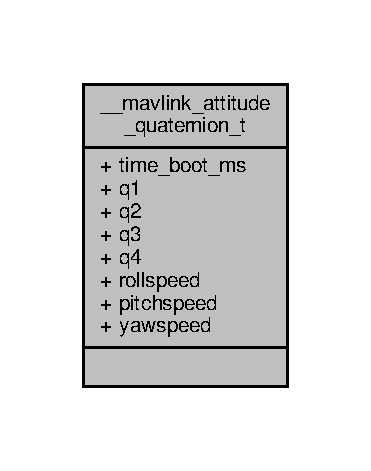
\includegraphics[width=178pt]{struct____mavlink__attitude__quaternion__t__coll__graph}
\end{center}
\end{figure}
\subsection*{Public Attributes}
\begin{DoxyCompactItemize}
\item 
\hypertarget{struct____mavlink__attitude__quaternion__t_af6846c94b303788cf54d7861a939ab15}{uint32\+\_\+t \hyperlink{struct____mavlink__attitude__quaternion__t_af6846c94b303788cf54d7861a939ab15}{time\+\_\+boot\+\_\+ms}}\label{struct____mavlink__attitude__quaternion__t_af6846c94b303788cf54d7861a939ab15}

\begin{DoxyCompactList}\small\item\em Timestamp (milliseconds since system boot) \end{DoxyCompactList}\item 
\hypertarget{struct____mavlink__attitude__quaternion__t_a54fd7b1cca2ab5e1b800bef5c7014b17}{float \hyperlink{struct____mavlink__attitude__quaternion__t_a54fd7b1cca2ab5e1b800bef5c7014b17}{q1}}\label{struct____mavlink__attitude__quaternion__t_a54fd7b1cca2ab5e1b800bef5c7014b17}

\begin{DoxyCompactList}\small\item\em Quaternion component 1. \end{DoxyCompactList}\item 
\hypertarget{struct____mavlink__attitude__quaternion__t_ad6451d99fa8f80bba96a47b3c2408255}{float \hyperlink{struct____mavlink__attitude__quaternion__t_ad6451d99fa8f80bba96a47b3c2408255}{q2}}\label{struct____mavlink__attitude__quaternion__t_ad6451d99fa8f80bba96a47b3c2408255}

\begin{DoxyCompactList}\small\item\em Quaternion component 2. \end{DoxyCompactList}\item 
\hypertarget{struct____mavlink__attitude__quaternion__t_a6ea5423090526626cf04041c929703d5}{float \hyperlink{struct____mavlink__attitude__quaternion__t_a6ea5423090526626cf04041c929703d5}{q3}}\label{struct____mavlink__attitude__quaternion__t_a6ea5423090526626cf04041c929703d5}

\begin{DoxyCompactList}\small\item\em Quaternion component 3. \end{DoxyCompactList}\item 
\hypertarget{struct____mavlink__attitude__quaternion__t_a4c78a9e744406f980fab7ff67613b14d}{float \hyperlink{struct____mavlink__attitude__quaternion__t_a4c78a9e744406f980fab7ff67613b14d}{q4}}\label{struct____mavlink__attitude__quaternion__t_a4c78a9e744406f980fab7ff67613b14d}

\begin{DoxyCompactList}\small\item\em Quaternion component 4. \end{DoxyCompactList}\item 
\hypertarget{struct____mavlink__attitude__quaternion__t_aa6ec530191df4da1f482533321684902}{float \hyperlink{struct____mavlink__attitude__quaternion__t_aa6ec530191df4da1f482533321684902}{rollspeed}}\label{struct____mavlink__attitude__quaternion__t_aa6ec530191df4da1f482533321684902}

\begin{DoxyCompactList}\small\item\em Roll angular speed (rad/s) \end{DoxyCompactList}\item 
\hypertarget{struct____mavlink__attitude__quaternion__t_ac77cd2999fca4230bf4fe7bcfe67c434}{float \hyperlink{struct____mavlink__attitude__quaternion__t_ac77cd2999fca4230bf4fe7bcfe67c434}{pitchspeed}}\label{struct____mavlink__attitude__quaternion__t_ac77cd2999fca4230bf4fe7bcfe67c434}

\begin{DoxyCompactList}\small\item\em Pitch angular speed (rad/s) \end{DoxyCompactList}\item 
\hypertarget{struct____mavlink__attitude__quaternion__t_a6e76b94100205e6f58df4232c1b4c32e}{float \hyperlink{struct____mavlink__attitude__quaternion__t_a6e76b94100205e6f58df4232c1b4c32e}{yawspeed}}\label{struct____mavlink__attitude__quaternion__t_a6e76b94100205e6f58df4232c1b4c32e}

\begin{DoxyCompactList}\small\item\em Yaw angular speed (rad/s) \end{DoxyCompactList}\end{DoxyCompactItemize}


The documentation for this struct was generated from the following file\+:\begin{DoxyCompactItemize}
\item 
/run/media/julien/\+Data/\+Documents/\+M\+A\+V\+R\+I\+C/\+M\+A\+V\+R\+I\+C\+\_\+\+Library/mavlink/include/common/mavlink\+\_\+msg\+\_\+attitude\+\_\+quaternion.\+h\end{DoxyCompactItemize}

\hypertarget{struct____mavlink__attitude__t}{\section{\+\_\+\+\_\+mavlink\+\_\+attitude\+\_\+t Struct Reference}
\label{struct____mavlink__attitude__t}\index{\+\_\+\+\_\+mavlink\+\_\+attitude\+\_\+t@{\+\_\+\+\_\+mavlink\+\_\+attitude\+\_\+t}}
}


Collaboration diagram for \+\_\+\+\_\+mavlink\+\_\+attitude\+\_\+t\+:
\nopagebreak
\begin{figure}[H]
\begin{center}
\leavevmode
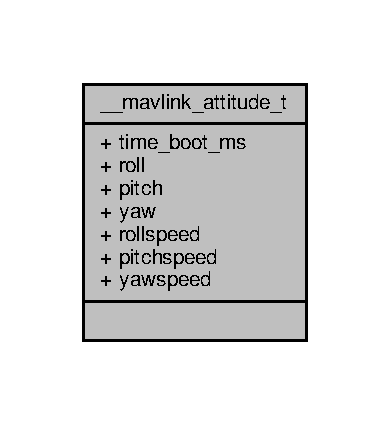
\includegraphics[width=187pt]{struct____mavlink__attitude__t__coll__graph}
\end{center}
\end{figure}
\subsection*{Public Attributes}
\begin{DoxyCompactItemize}
\item 
\hypertarget{struct____mavlink__attitude__t_a7330cabdd19ca8d3dc27ff1a6b585326}{uint32\+\_\+t \hyperlink{struct____mavlink__attitude__t_a7330cabdd19ca8d3dc27ff1a6b585326}{time\+\_\+boot\+\_\+ms}}\label{struct____mavlink__attitude__t_a7330cabdd19ca8d3dc27ff1a6b585326}

\begin{DoxyCompactList}\small\item\em Timestamp (milliseconds since system boot) \end{DoxyCompactList}\item 
\hypertarget{struct____mavlink__attitude__t_a5ac57ac7109bca27a72d5a4128a8010f}{float \hyperlink{struct____mavlink__attitude__t_a5ac57ac7109bca27a72d5a4128a8010f}{roll}}\label{struct____mavlink__attitude__t_a5ac57ac7109bca27a72d5a4128a8010f}

\begin{DoxyCompactList}\small\item\em Roll angle (rad, -\/pi..+pi) \end{DoxyCompactList}\item 
\hypertarget{struct____mavlink__attitude__t_ad9be17d1bb5941060e7c81634ebec51c}{float \hyperlink{struct____mavlink__attitude__t_ad9be17d1bb5941060e7c81634ebec51c}{pitch}}\label{struct____mavlink__attitude__t_ad9be17d1bb5941060e7c81634ebec51c}

\begin{DoxyCompactList}\small\item\em Pitch angle (rad, -\/pi..+pi) \end{DoxyCompactList}\item 
\hypertarget{struct____mavlink__attitude__t_a24ce486ebd7bde1558ad456684bcbd93}{float \hyperlink{struct____mavlink__attitude__t_a24ce486ebd7bde1558ad456684bcbd93}{yaw}}\label{struct____mavlink__attitude__t_a24ce486ebd7bde1558ad456684bcbd93}

\begin{DoxyCompactList}\small\item\em Yaw angle (rad, -\/pi..+pi) \end{DoxyCompactList}\item 
\hypertarget{struct____mavlink__attitude__t_ae46e19a3dc0bde80d9a0eddbc0f9315d}{float \hyperlink{struct____mavlink__attitude__t_ae46e19a3dc0bde80d9a0eddbc0f9315d}{rollspeed}}\label{struct____mavlink__attitude__t_ae46e19a3dc0bde80d9a0eddbc0f9315d}

\begin{DoxyCompactList}\small\item\em Roll angular speed (rad/s) \end{DoxyCompactList}\item 
\hypertarget{struct____mavlink__attitude__t_a6496f9102154455ef47db7c0cab5c141}{float \hyperlink{struct____mavlink__attitude__t_a6496f9102154455ef47db7c0cab5c141}{pitchspeed}}\label{struct____mavlink__attitude__t_a6496f9102154455ef47db7c0cab5c141}

\begin{DoxyCompactList}\small\item\em Pitch angular speed (rad/s) \end{DoxyCompactList}\item 
\hypertarget{struct____mavlink__attitude__t_a2a6cd5ab90b6c939dec690ebf7000101}{float \hyperlink{struct____mavlink__attitude__t_a2a6cd5ab90b6c939dec690ebf7000101}{yawspeed}}\label{struct____mavlink__attitude__t_a2a6cd5ab90b6c939dec690ebf7000101}

\begin{DoxyCompactList}\small\item\em Yaw angular speed (rad/s) \end{DoxyCompactList}\end{DoxyCompactItemize}


The documentation for this struct was generated from the following file\+:\begin{DoxyCompactItemize}
\item 
/run/media/julien/\+Data/\+Documents/\+M\+A\+V\+R\+I\+C/\+M\+A\+V\+R\+I\+C\+\_\+\+Library/mavlink/include/common/mavlink\+\_\+msg\+\_\+attitude.\+h\end{DoxyCompactItemize}

\hypertarget{struct____mavlink__auth__key__t}{\section{\+\_\+\+\_\+mavlink\+\_\+auth\+\_\+key\+\_\+t Struct Reference}
\label{struct____mavlink__auth__key__t}\index{\+\_\+\+\_\+mavlink\+\_\+auth\+\_\+key\+\_\+t@{\+\_\+\+\_\+mavlink\+\_\+auth\+\_\+key\+\_\+t}}
}


Collaboration diagram for \+\_\+\+\_\+mavlink\+\_\+auth\+\_\+key\+\_\+t\+:
\nopagebreak
\begin{figure}[H]
\begin{center}
\leavevmode
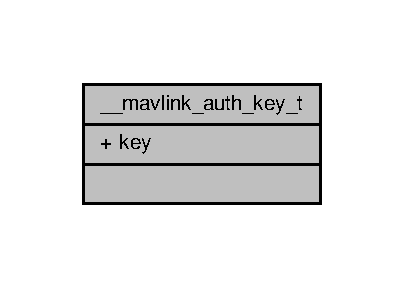
\includegraphics[width=194pt]{struct____mavlink__auth__key__t__coll__graph}
\end{center}
\end{figure}
\subsection*{Public Attributes}
\begin{DoxyCompactItemize}
\item 
\hypertarget{struct____mavlink__auth__key__t_a543d2ad5a931c4d983abb287a9da1f06}{char \hyperlink{struct____mavlink__auth__key__t_a543d2ad5a931c4d983abb287a9da1f06}{key} \mbox{[}32\mbox{]}}\label{struct____mavlink__auth__key__t_a543d2ad5a931c4d983abb287a9da1f06}

\begin{DoxyCompactList}\small\item\em key \end{DoxyCompactList}\end{DoxyCompactItemize}


The documentation for this struct was generated from the following file\+:\begin{DoxyCompactItemize}
\item 
/run/media/julien/\+Data/\+Documents/\+M\+A\+V\+R\+I\+C/\+M\+A\+V\+R\+I\+C\+\_\+\+Library/mavlink/include/common/mavlink\+\_\+msg\+\_\+auth\+\_\+key.\+h\end{DoxyCompactItemize}

\hypertarget{struct____mavlink__battery__status__t}{\section{\+\_\+\+\_\+mavlink\+\_\+battery\+\_\+status\+\_\+t Struct Reference}
\label{struct____mavlink__battery__status__t}\index{\+\_\+\+\_\+mavlink\+\_\+battery\+\_\+status\+\_\+t@{\+\_\+\+\_\+mavlink\+\_\+battery\+\_\+status\+\_\+t}}
}


Collaboration diagram for \+\_\+\+\_\+mavlink\+\_\+battery\+\_\+status\+\_\+t\+:
\nopagebreak
\begin{figure}[H]
\begin{center}
\leavevmode
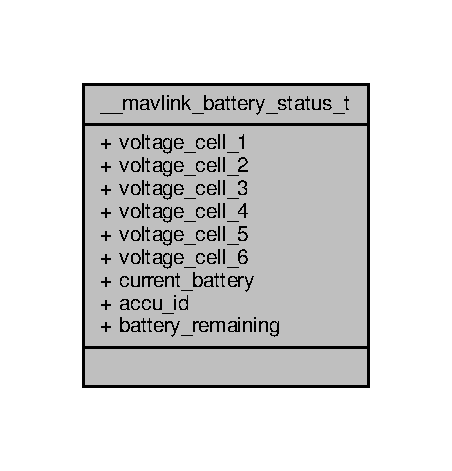
\includegraphics[width=217pt]{struct____mavlink__battery__status__t__coll__graph}
\end{center}
\end{figure}
\subsection*{Public Attributes}
\begin{DoxyCompactItemize}
\item 
\hypertarget{struct____mavlink__battery__status__t_adaeb25259ebf6a9a53a9cb4edc20b314}{uint16\+\_\+t \hyperlink{struct____mavlink__battery__status__t_adaeb25259ebf6a9a53a9cb4edc20b314}{voltage\+\_\+cell\+\_\+1}}\label{struct____mavlink__battery__status__t_adaeb25259ebf6a9a53a9cb4edc20b314}

\begin{DoxyCompactList}\small\item\em Battery voltage of cell 1, in millivolts (1 = 1 millivolt) \end{DoxyCompactList}\item 
\hypertarget{struct____mavlink__battery__status__t_ab785f30613bb2406144f9d923dd0f44c}{uint16\+\_\+t \hyperlink{struct____mavlink__battery__status__t_ab785f30613bb2406144f9d923dd0f44c}{voltage\+\_\+cell\+\_\+2}}\label{struct____mavlink__battery__status__t_ab785f30613bb2406144f9d923dd0f44c}

\begin{DoxyCompactList}\small\item\em Battery voltage of cell 2, in millivolts (1 = 1 millivolt), -\/1\+: no cell. \end{DoxyCompactList}\item 
\hypertarget{struct____mavlink__battery__status__t_addc83e20e1b3a4f56d9718cdfa0b94f9}{uint16\+\_\+t \hyperlink{struct____mavlink__battery__status__t_addc83e20e1b3a4f56d9718cdfa0b94f9}{voltage\+\_\+cell\+\_\+3}}\label{struct____mavlink__battery__status__t_addc83e20e1b3a4f56d9718cdfa0b94f9}

\begin{DoxyCompactList}\small\item\em Battery voltage of cell 3, in millivolts (1 = 1 millivolt), -\/1\+: no cell. \end{DoxyCompactList}\item 
\hypertarget{struct____mavlink__battery__status__t_afdd7db92c49d50189e101c78d120b64b}{uint16\+\_\+t \hyperlink{struct____mavlink__battery__status__t_afdd7db92c49d50189e101c78d120b64b}{voltage\+\_\+cell\+\_\+4}}\label{struct____mavlink__battery__status__t_afdd7db92c49d50189e101c78d120b64b}

\begin{DoxyCompactList}\small\item\em Battery voltage of cell 4, in millivolts (1 = 1 millivolt), -\/1\+: no cell. \end{DoxyCompactList}\item 
\hypertarget{struct____mavlink__battery__status__t_a3a077490266e57c0f0e63d81079bfc86}{uint16\+\_\+t \hyperlink{struct____mavlink__battery__status__t_a3a077490266e57c0f0e63d81079bfc86}{voltage\+\_\+cell\+\_\+5}}\label{struct____mavlink__battery__status__t_a3a077490266e57c0f0e63d81079bfc86}

\begin{DoxyCompactList}\small\item\em Battery voltage of cell 5, in millivolts (1 = 1 millivolt), -\/1\+: no cell. \end{DoxyCompactList}\item 
\hypertarget{struct____mavlink__battery__status__t_ac1e3680e0cad76eab6833c1c62cfefb5}{uint16\+\_\+t \hyperlink{struct____mavlink__battery__status__t_ac1e3680e0cad76eab6833c1c62cfefb5}{voltage\+\_\+cell\+\_\+6}}\label{struct____mavlink__battery__status__t_ac1e3680e0cad76eab6833c1c62cfefb5}

\begin{DoxyCompactList}\small\item\em Battery voltage of cell 6, in millivolts (1 = 1 millivolt), -\/1\+: no cell. \end{DoxyCompactList}\item 
\hypertarget{struct____mavlink__battery__status__t_a1577349498c9881468031a20cd2faeae}{int16\+\_\+t \hyperlink{struct____mavlink__battery__status__t_a1577349498c9881468031a20cd2faeae}{current\+\_\+battery}}\label{struct____mavlink__battery__status__t_a1577349498c9881468031a20cd2faeae}

\begin{DoxyCompactList}\small\item\em Battery current, in 10$\ast$milliamperes (1 = 10 milliampere), -\/1\+: autopilot does not measure the current. \end{DoxyCompactList}\item 
\hypertarget{struct____mavlink__battery__status__t_afbf96cd532816d0da0228c63dfabce0d}{uint8\+\_\+t \hyperlink{struct____mavlink__battery__status__t_afbf96cd532816d0da0228c63dfabce0d}{accu\+\_\+id}}\label{struct____mavlink__battery__status__t_afbf96cd532816d0da0228c63dfabce0d}

\begin{DoxyCompactList}\small\item\em Accupack I\+D. \end{DoxyCompactList}\item 
\hypertarget{struct____mavlink__battery__status__t_aa2aa73e1a73123460a4da3e3918ca434}{int8\+\_\+t \hyperlink{struct____mavlink__battery__status__t_aa2aa73e1a73123460a4da3e3918ca434}{battery\+\_\+remaining}}\label{struct____mavlink__battery__status__t_aa2aa73e1a73123460a4da3e3918ca434}

\begin{DoxyCompactList}\small\item\em Remaining battery energy\+: (0\%\+: 0, 100\%\+: 100), -\/1\+: autopilot does not estimate the remaining battery. \end{DoxyCompactList}\end{DoxyCompactItemize}


The documentation for this struct was generated from the following file\+:\begin{DoxyCompactItemize}
\item 
/run/media/julien/\+Data/\+Documents/\+M\+A\+V\+R\+I\+C/\+M\+A\+V\+R\+I\+C\+\_\+\+Library/mavlink/include/common/mavlink\+\_\+msg\+\_\+battery\+\_\+status.\+h\end{DoxyCompactItemize}

\hypertarget{union____mavlink__bitfield}{\section{\+\_\+\+\_\+mavlink\+\_\+bitfield Union Reference}
\label{union____mavlink__bitfield}\index{\+\_\+\+\_\+mavlink\+\_\+bitfield@{\+\_\+\+\_\+mavlink\+\_\+bitfield}}
}


Collaboration diagram for \+\_\+\+\_\+mavlink\+\_\+bitfield\+:
\nopagebreak
\begin{figure}[H]
\begin{center}
\leavevmode
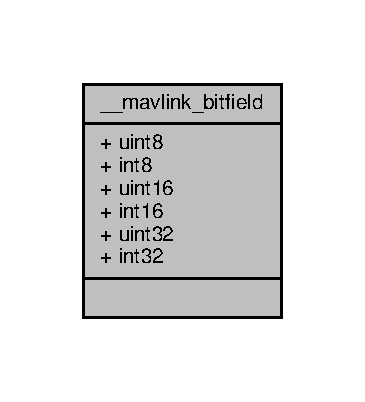
\includegraphics[width=175pt]{union____mavlink__bitfield__coll__graph}
\end{center}
\end{figure}
\subsection*{Public Attributes}
\begin{DoxyCompactItemize}
\item 
\hypertarget{union____mavlink__bitfield_ade669a5f63c53f0d61f636eff94417c0}{uint8\+\_\+t {\bfseries uint8}}\label{union____mavlink__bitfield_ade669a5f63c53f0d61f636eff94417c0}

\item 
\hypertarget{union____mavlink__bitfield_a50a846d427d7a1d7dc79235c87597622}{int8\+\_\+t {\bfseries int8}}\label{union____mavlink__bitfield_a50a846d427d7a1d7dc79235c87597622}

\item 
\hypertarget{union____mavlink__bitfield_a0ca76ce4a09ee26387e50b6702c17894}{uint16\+\_\+t {\bfseries uint16}}\label{union____mavlink__bitfield_a0ca76ce4a09ee26387e50b6702c17894}

\item 
\hypertarget{union____mavlink__bitfield_a99cd7f966d8a59b29d05197b39c5b229}{int16\+\_\+t {\bfseries int16}}\label{union____mavlink__bitfield_a99cd7f966d8a59b29d05197b39c5b229}

\item 
\hypertarget{union____mavlink__bitfield_ab43ed56310c2d778ebaa7a5a21cb6587}{uint32\+\_\+t {\bfseries uint32}}\label{union____mavlink__bitfield_ab43ed56310c2d778ebaa7a5a21cb6587}

\item 
\hypertarget{union____mavlink__bitfield_a07bd702e8b91679a25e632ad90d0a1ec}{int32\+\_\+t {\bfseries int32}}\label{union____mavlink__bitfield_a07bd702e8b91679a25e632ad90d0a1ec}

\end{DoxyCompactItemize}


The documentation for this union was generated from the following file\+:\begin{DoxyCompactItemize}
\item 
/run/media/julien/\+Data/\+Documents/\+M\+A\+V\+R\+I\+C/\+M\+A\+V\+R\+I\+C\+\_\+\+Library/mavlink/include/mavlink\+\_\+helpers.\+h\end{DoxyCompactItemize}

\hypertarget{struct____mavlink__change__operator__control__ack__t}{\section{\+\_\+\+\_\+mavlink\+\_\+change\+\_\+operator\+\_\+control\+\_\+ack\+\_\+t Struct Reference}
\label{struct____mavlink__change__operator__control__ack__t}\index{\+\_\+\+\_\+mavlink\+\_\+change\+\_\+operator\+\_\+control\+\_\+ack\+\_\+t@{\+\_\+\+\_\+mavlink\+\_\+change\+\_\+operator\+\_\+control\+\_\+ack\+\_\+t}}
}


Collaboration diagram for \+\_\+\+\_\+mavlink\+\_\+change\+\_\+operator\+\_\+control\+\_\+ack\+\_\+t\+:
\nopagebreak
\begin{figure}[H]
\begin{center}
\leavevmode
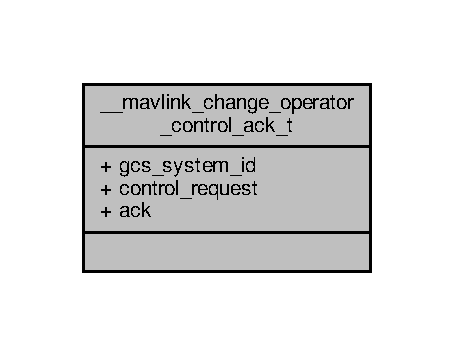
\includegraphics[width=218pt]{struct____mavlink__change__operator__control__ack__t__coll__graph}
\end{center}
\end{figure}
\subsection*{Public Attributes}
\begin{DoxyCompactItemize}
\item 
\hypertarget{struct____mavlink__change__operator__control__ack__t_adb8f2a279063a0615952eda9f2b3dc24}{uint8\+\_\+t \hyperlink{struct____mavlink__change__operator__control__ack__t_adb8f2a279063a0615952eda9f2b3dc24}{gcs\+\_\+system\+\_\+id}}\label{struct____mavlink__change__operator__control__ack__t_adb8f2a279063a0615952eda9f2b3dc24}

\begin{DoxyCompactList}\small\item\em I\+D of the G\+C\+S this message. \end{DoxyCompactList}\item 
\hypertarget{struct____mavlink__change__operator__control__ack__t_a3b0abe5ae412967c3341c6e90f09d0d6}{uint8\+\_\+t \hyperlink{struct____mavlink__change__operator__control__ack__t_a3b0abe5ae412967c3341c6e90f09d0d6}{control\+\_\+request}}\label{struct____mavlink__change__operator__control__ack__t_a3b0abe5ae412967c3341c6e90f09d0d6}

\begin{DoxyCompactList}\small\item\em 0\+: request control of this M\+A\+V, 1\+: Release control of this M\+A\+V \end{DoxyCompactList}\item 
\hypertarget{struct____mavlink__change__operator__control__ack__t_a420017052e533270a67f82a663bc07fa}{uint8\+\_\+t \hyperlink{struct____mavlink__change__operator__control__ack__t_a420017052e533270a67f82a663bc07fa}{ack}}\label{struct____mavlink__change__operator__control__ack__t_a420017052e533270a67f82a663bc07fa}

\begin{DoxyCompactList}\small\item\em 0\+: A\+C\+K, 1\+: N\+A\+C\+K\+: Wrong passkey, 2\+: N\+A\+C\+K\+: Unsupported passkey encryption method, 3\+: N\+A\+C\+K\+: Already under control \end{DoxyCompactList}\end{DoxyCompactItemize}


The documentation for this struct was generated from the following file\+:\begin{DoxyCompactItemize}
\item 
/run/media/julien/\+Data/\+Documents/\+M\+A\+V\+R\+I\+C/\+M\+A\+V\+R\+I\+C\+\_\+\+Library/mavlink/include/common/mavlink\+\_\+msg\+\_\+change\+\_\+operator\+\_\+control\+\_\+ack.\+h\end{DoxyCompactItemize}

\hypertarget{struct____mavlink__change__operator__control__t}{\section{\+\_\+\+\_\+mavlink\+\_\+change\+\_\+operator\+\_\+control\+\_\+t Struct Reference}
\label{struct____mavlink__change__operator__control__t}\index{\+\_\+\+\_\+mavlink\+\_\+change\+\_\+operator\+\_\+control\+\_\+t@{\+\_\+\+\_\+mavlink\+\_\+change\+\_\+operator\+\_\+control\+\_\+t}}
}


Collaboration diagram for \+\_\+\+\_\+mavlink\+\_\+change\+\_\+operator\+\_\+control\+\_\+t\+:
\nopagebreak
\begin{figure}[H]
\begin{center}
\leavevmode
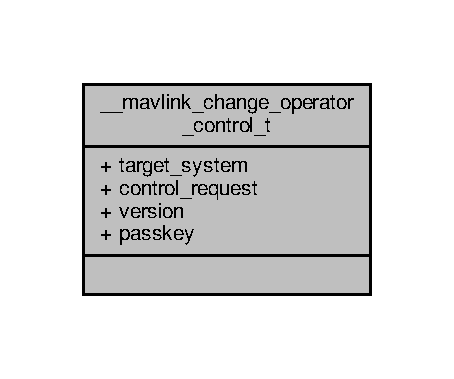
\includegraphics[width=218pt]{struct____mavlink__change__operator__control__t__coll__graph}
\end{center}
\end{figure}
\subsection*{Public Attributes}
\begin{DoxyCompactItemize}
\item 
\hypertarget{struct____mavlink__change__operator__control__t_ac68f72fea3c066f00e0ccd0b978d119a}{uint8\+\_\+t \hyperlink{struct____mavlink__change__operator__control__t_ac68f72fea3c066f00e0ccd0b978d119a}{target\+\_\+system}}\label{struct____mavlink__change__operator__control__t_ac68f72fea3c066f00e0ccd0b978d119a}

\begin{DoxyCompactList}\small\item\em System the G\+C\+S requests control for. \end{DoxyCompactList}\item 
\hypertarget{struct____mavlink__change__operator__control__t_aef19fec531d51e7a3f57fe09a7f74c06}{uint8\+\_\+t \hyperlink{struct____mavlink__change__operator__control__t_aef19fec531d51e7a3f57fe09a7f74c06}{control\+\_\+request}}\label{struct____mavlink__change__operator__control__t_aef19fec531d51e7a3f57fe09a7f74c06}

\begin{DoxyCompactList}\small\item\em 0\+: request control of this M\+A\+V, 1\+: Release control of this M\+A\+V \end{DoxyCompactList}\item 
\hypertarget{struct____mavlink__change__operator__control__t_a033ed1de1f96ee19a64572952e29da39}{uint8\+\_\+t \hyperlink{struct____mavlink__change__operator__control__t_a033ed1de1f96ee19a64572952e29da39}{version}}\label{struct____mavlink__change__operator__control__t_a033ed1de1f96ee19a64572952e29da39}

\begin{DoxyCompactList}\small\item\em 0\+: key as plaintext, 1-\/255\+: future, different hashing/encryption variants. The G\+C\+S should in general use the safest mode possible initially and then gradually move down the encryption level if it gets a N\+A\+C\+K message indicating an encryption mismatch. \end{DoxyCompactList}\item 
\hypertarget{struct____mavlink__change__operator__control__t_a6d90be6cd729954dbc7fa10d440f9cd2}{char \hyperlink{struct____mavlink__change__operator__control__t_a6d90be6cd729954dbc7fa10d440f9cd2}{passkey} \mbox{[}25\mbox{]}}\label{struct____mavlink__change__operator__control__t_a6d90be6cd729954dbc7fa10d440f9cd2}

\begin{DoxyCompactList}\small\item\em Password / Key, depending on version plaintext or encrypted. 25 or less characters, N\+U\+L\+L terminated. The characters may involve A-\/\+Z, a-\/z, 0-\/9, and \char`\"{}!?,.-\/\char`\"{}. \end{DoxyCompactList}\end{DoxyCompactItemize}


The documentation for this struct was generated from the following file\+:\begin{DoxyCompactItemize}
\item 
/run/media/julien/\+Data/\+Documents/\+M\+A\+V\+R\+I\+C/\+M\+A\+V\+R\+I\+C\+\_\+\+Library/mavlink/include/common/mavlink\+\_\+msg\+\_\+change\+\_\+operator\+\_\+control.\+h\end{DoxyCompactItemize}

\hypertarget{struct____mavlink__command__ack__t}{\section{\+\_\+\+\_\+mavlink\+\_\+command\+\_\+ack\+\_\+t Struct Reference}
\label{struct____mavlink__command__ack__t}\index{\+\_\+\+\_\+mavlink\+\_\+command\+\_\+ack\+\_\+t@{\+\_\+\+\_\+mavlink\+\_\+command\+\_\+ack\+\_\+t}}
}


Collaboration diagram for \+\_\+\+\_\+mavlink\+\_\+command\+\_\+ack\+\_\+t\+:
\nopagebreak
\begin{figure}[H]
\begin{center}
\leavevmode
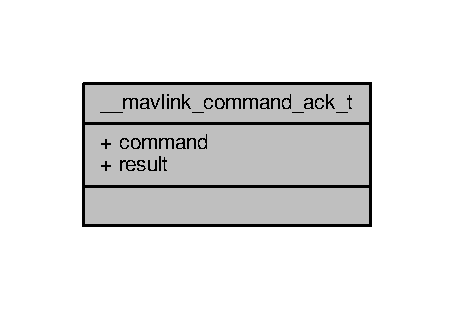
\includegraphics[width=218pt]{struct____mavlink__command__ack__t__coll__graph}
\end{center}
\end{figure}
\subsection*{Public Attributes}
\begin{DoxyCompactItemize}
\item 
\hypertarget{struct____mavlink__command__ack__t_a4c63e16e7da216bf952f61e33a4ad5e7}{uint16\+\_\+t \hyperlink{struct____mavlink__command__ack__t_a4c63e16e7da216bf952f61e33a4ad5e7}{command}}\label{struct____mavlink__command__ack__t_a4c63e16e7da216bf952f61e33a4ad5e7}

\begin{DoxyCompactList}\small\item\em Command I\+D, as defined by M\+A\+V\+\_\+\+C\+M\+D enum. \end{DoxyCompactList}\item 
\hypertarget{struct____mavlink__command__ack__t_ae8165e8e4f7a1438977e1a7edd646b69}{uint8\+\_\+t \hyperlink{struct____mavlink__command__ack__t_ae8165e8e4f7a1438977e1a7edd646b69}{result}}\label{struct____mavlink__command__ack__t_ae8165e8e4f7a1438977e1a7edd646b69}

\begin{DoxyCompactList}\small\item\em See M\+A\+V\+\_\+\+R\+E\+S\+U\+L\+T enum. \end{DoxyCompactList}\end{DoxyCompactItemize}


The documentation for this struct was generated from the following file\+:\begin{DoxyCompactItemize}
\item 
/run/media/julien/\+Data/\+Documents/\+M\+A\+V\+R\+I\+C/\+M\+A\+V\+R\+I\+C\+\_\+\+Library/mavlink/include/common/mavlink\+\_\+msg\+\_\+command\+\_\+ack.\+h\end{DoxyCompactItemize}

\hypertarget{struct____mavlink__command__long__t}{\section{\+\_\+\+\_\+mavlink\+\_\+command\+\_\+long\+\_\+t Struct Reference}
\label{struct____mavlink__command__long__t}\index{\+\_\+\+\_\+mavlink\+\_\+command\+\_\+long\+\_\+t@{\+\_\+\+\_\+mavlink\+\_\+command\+\_\+long\+\_\+t}}
}


Collaboration diagram for \+\_\+\+\_\+mavlink\+\_\+command\+\_\+long\+\_\+t\+:
\nopagebreak
\begin{figure}[H]
\begin{center}
\leavevmode
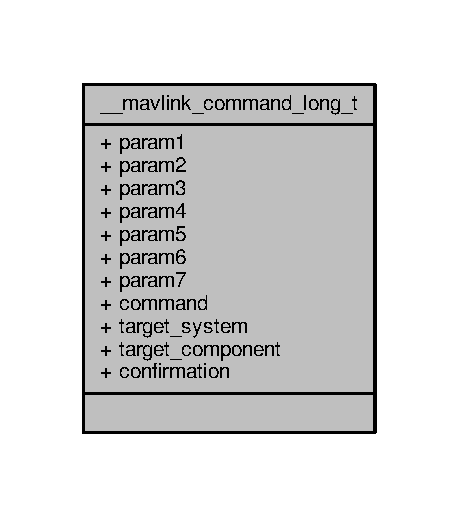
\includegraphics[width=220pt]{struct____mavlink__command__long__t__coll__graph}
\end{center}
\end{figure}
\subsection*{Public Attributes}
\begin{DoxyCompactItemize}
\item 
\hypertarget{struct____mavlink__command__long__t_a8bb82d921422fd825276bbc43502fc77}{float \hyperlink{struct____mavlink__command__long__t_a8bb82d921422fd825276bbc43502fc77}{param1}}\label{struct____mavlink__command__long__t_a8bb82d921422fd825276bbc43502fc77}

\begin{DoxyCompactList}\small\item\em Parameter 1, as defined by M\+A\+V\+\_\+\+C\+M\+D enum. \end{DoxyCompactList}\item 
\hypertarget{struct____mavlink__command__long__t_a715bfae8c34e8882b82efbb2bd0e580c}{float \hyperlink{struct____mavlink__command__long__t_a715bfae8c34e8882b82efbb2bd0e580c}{param2}}\label{struct____mavlink__command__long__t_a715bfae8c34e8882b82efbb2bd0e580c}

\begin{DoxyCompactList}\small\item\em Parameter 2, as defined by M\+A\+V\+\_\+\+C\+M\+D enum. \end{DoxyCompactList}\item 
\hypertarget{struct____mavlink__command__long__t_a9b11618cd6d409944727cfcc0d637f72}{float \hyperlink{struct____mavlink__command__long__t_a9b11618cd6d409944727cfcc0d637f72}{param3}}\label{struct____mavlink__command__long__t_a9b11618cd6d409944727cfcc0d637f72}

\begin{DoxyCompactList}\small\item\em Parameter 3, as defined by M\+A\+V\+\_\+\+C\+M\+D enum. \end{DoxyCompactList}\item 
\hypertarget{struct____mavlink__command__long__t_a1448f543670b7a8973c6461254cce429}{float \hyperlink{struct____mavlink__command__long__t_a1448f543670b7a8973c6461254cce429}{param4}}\label{struct____mavlink__command__long__t_a1448f543670b7a8973c6461254cce429}

\begin{DoxyCompactList}\small\item\em Parameter 4, as defined by M\+A\+V\+\_\+\+C\+M\+D enum. \end{DoxyCompactList}\item 
\hypertarget{struct____mavlink__command__long__t_a9c74f309b82fed5527bf1e7732424f21}{float \hyperlink{struct____mavlink__command__long__t_a9c74f309b82fed5527bf1e7732424f21}{param5}}\label{struct____mavlink__command__long__t_a9c74f309b82fed5527bf1e7732424f21}

\begin{DoxyCompactList}\small\item\em Parameter 5, as defined by M\+A\+V\+\_\+\+C\+M\+D enum. \end{DoxyCompactList}\item 
\hypertarget{struct____mavlink__command__long__t_ad75daa212f56fd47cd0956f8dc4fdbd5}{float \hyperlink{struct____mavlink__command__long__t_ad75daa212f56fd47cd0956f8dc4fdbd5}{param6}}\label{struct____mavlink__command__long__t_ad75daa212f56fd47cd0956f8dc4fdbd5}

\begin{DoxyCompactList}\small\item\em Parameter 6, as defined by M\+A\+V\+\_\+\+C\+M\+D enum. \end{DoxyCompactList}\item 
\hypertarget{struct____mavlink__command__long__t_a1bf675e543b14770e7c410adb9d3d21e}{float \hyperlink{struct____mavlink__command__long__t_a1bf675e543b14770e7c410adb9d3d21e}{param7}}\label{struct____mavlink__command__long__t_a1bf675e543b14770e7c410adb9d3d21e}

\begin{DoxyCompactList}\small\item\em Parameter 7, as defined by M\+A\+V\+\_\+\+C\+M\+D enum. \end{DoxyCompactList}\item 
\hypertarget{struct____mavlink__command__long__t_a059e44ecfa8fbb9f11543a81145265cf}{uint16\+\_\+t \hyperlink{struct____mavlink__command__long__t_a059e44ecfa8fbb9f11543a81145265cf}{command}}\label{struct____mavlink__command__long__t_a059e44ecfa8fbb9f11543a81145265cf}

\begin{DoxyCompactList}\small\item\em Command I\+D, as defined by M\+A\+V\+\_\+\+C\+M\+D enum. \end{DoxyCompactList}\item 
\hypertarget{struct____mavlink__command__long__t_a705313e3359248c2e2b77d71b99a5d3d}{uint8\+\_\+t \hyperlink{struct____mavlink__command__long__t_a705313e3359248c2e2b77d71b99a5d3d}{target\+\_\+system}}\label{struct____mavlink__command__long__t_a705313e3359248c2e2b77d71b99a5d3d}

\begin{DoxyCompactList}\small\item\em System which should execute the command. \end{DoxyCompactList}\item 
\hypertarget{struct____mavlink__command__long__t_ab2e28f55169c5076999e2c941bafce39}{uint8\+\_\+t \hyperlink{struct____mavlink__command__long__t_ab2e28f55169c5076999e2c941bafce39}{target\+\_\+component}}\label{struct____mavlink__command__long__t_ab2e28f55169c5076999e2c941bafce39}

\begin{DoxyCompactList}\small\item\em Component which should execute the command, 0 for all components. \end{DoxyCompactList}\item 
\hypertarget{struct____mavlink__command__long__t_a79ec42e9308bf4cc44c64ae939fe1d61}{uint8\+\_\+t \hyperlink{struct____mavlink__command__long__t_a79ec42e9308bf4cc44c64ae939fe1d61}{confirmation}}\label{struct____mavlink__command__long__t_a79ec42e9308bf4cc44c64ae939fe1d61}

\begin{DoxyCompactList}\small\item\em 0\+: First transmission of this command. 1-\/255\+: Confirmation transmissions (e.\+g. for kill command) \end{DoxyCompactList}\end{DoxyCompactItemize}


The documentation for this struct was generated from the following file\+:\begin{DoxyCompactItemize}
\item 
/run/media/julien/\+Data/\+Documents/\+M\+A\+V\+R\+I\+C/\+M\+A\+V\+R\+I\+C\+\_\+\+Library/mavlink/include/common/mavlink\+\_\+msg\+\_\+command\+\_\+long.\+h\end{DoxyCompactItemize}

\hypertarget{struct____mavlink__data__stream__t}{\section{\+\_\+\+\_\+mavlink\+\_\+data\+\_\+stream\+\_\+t Struct Reference}
\label{struct____mavlink__data__stream__t}\index{\+\_\+\+\_\+mavlink\+\_\+data\+\_\+stream\+\_\+t@{\+\_\+\+\_\+mavlink\+\_\+data\+\_\+stream\+\_\+t}}
}


Collaboration diagram for \+\_\+\+\_\+mavlink\+\_\+data\+\_\+stream\+\_\+t\+:
\nopagebreak
\begin{figure}[H]
\begin{center}
\leavevmode
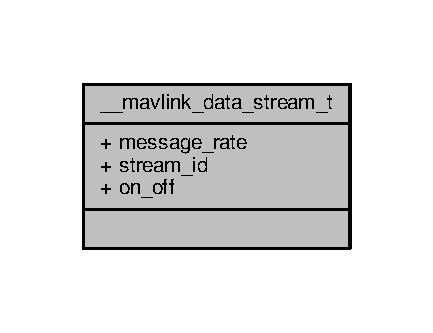
\includegraphics[width=208pt]{struct____mavlink__data__stream__t__coll__graph}
\end{center}
\end{figure}
\subsection*{Public Attributes}
\begin{DoxyCompactItemize}
\item 
\hypertarget{struct____mavlink__data__stream__t_a351a00b81ef679d4fa73048257494bbc}{uint16\+\_\+t \hyperlink{struct____mavlink__data__stream__t_a351a00b81ef679d4fa73048257494bbc}{message\+\_\+rate}}\label{struct____mavlink__data__stream__t_a351a00b81ef679d4fa73048257494bbc}

\begin{DoxyCompactList}\small\item\em The requested interval between two messages of this type. \end{DoxyCompactList}\item 
\hypertarget{struct____mavlink__data__stream__t_aaac4584f5e5677fe70edee1c53565b53}{uint8\+\_\+t \hyperlink{struct____mavlink__data__stream__t_aaac4584f5e5677fe70edee1c53565b53}{stream\+\_\+id}}\label{struct____mavlink__data__stream__t_aaac4584f5e5677fe70edee1c53565b53}

\begin{DoxyCompactList}\small\item\em The I\+D of the requested data stream. \end{DoxyCompactList}\item 
\hypertarget{struct____mavlink__data__stream__t_ae0ec7bd3a3fd38496e2a6aaa3b39daca}{uint8\+\_\+t \hyperlink{struct____mavlink__data__stream__t_ae0ec7bd3a3fd38496e2a6aaa3b39daca}{on\+\_\+off}}\label{struct____mavlink__data__stream__t_ae0ec7bd3a3fd38496e2a6aaa3b39daca}

\begin{DoxyCompactList}\small\item\em 1 stream is enabled, 0 stream is stopped. \end{DoxyCompactList}\end{DoxyCompactItemize}


The documentation for this struct was generated from the following file\+:\begin{DoxyCompactItemize}
\item 
/run/media/julien/\+Data/\+Documents/\+M\+A\+V\+R\+I\+C/\+M\+A\+V\+R\+I\+C\+\_\+\+Library/mavlink/include/common/mavlink\+\_\+msg\+\_\+data\+\_\+stream.\+h\end{DoxyCompactItemize}

\hypertarget{struct____mavlink__debug__t}{\section{\+\_\+\+\_\+mavlink\+\_\+debug\+\_\+t Struct Reference}
\label{struct____mavlink__debug__t}\index{\+\_\+\+\_\+mavlink\+\_\+debug\+\_\+t@{\+\_\+\+\_\+mavlink\+\_\+debug\+\_\+t}}
}


Collaboration diagram for \+\_\+\+\_\+mavlink\+\_\+debug\+\_\+t\+:
\nopagebreak
\begin{figure}[H]
\begin{center}
\leavevmode
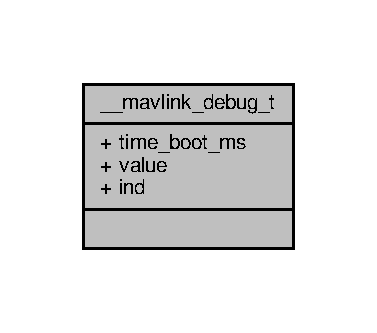
\includegraphics[width=181pt]{struct____mavlink__debug__t__coll__graph}
\end{center}
\end{figure}
\subsection*{Public Attributes}
\begin{DoxyCompactItemize}
\item 
\hypertarget{struct____mavlink__debug__t_afc1d1057d77ded488ac7b5034411604c}{uint32\+\_\+t \hyperlink{struct____mavlink__debug__t_afc1d1057d77ded488ac7b5034411604c}{time\+\_\+boot\+\_\+ms}}\label{struct____mavlink__debug__t_afc1d1057d77ded488ac7b5034411604c}

\begin{DoxyCompactList}\small\item\em Timestamp (milliseconds since system boot) \end{DoxyCompactList}\item 
\hypertarget{struct____mavlink__debug__t_aef9d0e91db46dff84494856146dcbcbe}{float \hyperlink{struct____mavlink__debug__t_aef9d0e91db46dff84494856146dcbcbe}{value}}\label{struct____mavlink__debug__t_aef9d0e91db46dff84494856146dcbcbe}

\begin{DoxyCompactList}\small\item\em D\+E\+B\+U\+G value. \end{DoxyCompactList}\item 
\hypertarget{struct____mavlink__debug__t_a540aecd3c98dd395f80edd92acab7c3d}{uint8\+\_\+t \hyperlink{struct____mavlink__debug__t_a540aecd3c98dd395f80edd92acab7c3d}{ind}}\label{struct____mavlink__debug__t_a540aecd3c98dd395f80edd92acab7c3d}

\begin{DoxyCompactList}\small\item\em index of debug variable \end{DoxyCompactList}\end{DoxyCompactItemize}


The documentation for this struct was generated from the following file\+:\begin{DoxyCompactItemize}
\item 
/run/media/julien/\+Data/\+Documents/\+M\+A\+V\+R\+I\+C/\+M\+A\+V\+R\+I\+C\+\_\+\+Library/mavlink/include/common/mavlink\+\_\+msg\+\_\+debug.\+h\end{DoxyCompactItemize}

\hypertarget{struct____mavlink__debug__vect__t}{\section{\+\_\+\+\_\+mavlink\+\_\+debug\+\_\+vect\+\_\+t Struct Reference}
\label{struct____mavlink__debug__vect__t}\index{\+\_\+\+\_\+mavlink\+\_\+debug\+\_\+vect\+\_\+t@{\+\_\+\+\_\+mavlink\+\_\+debug\+\_\+vect\+\_\+t}}
}


Collaboration diagram for \+\_\+\+\_\+mavlink\+\_\+debug\+\_\+vect\+\_\+t\+:
\nopagebreak
\begin{figure}[H]
\begin{center}
\leavevmode
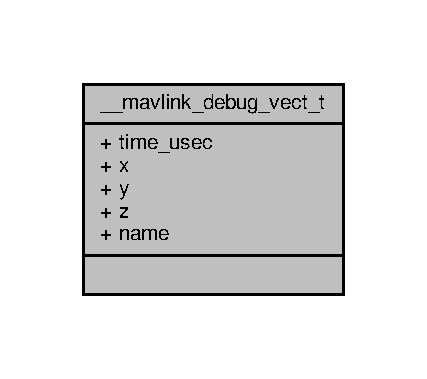
\includegraphics[width=205pt]{struct____mavlink__debug__vect__t__coll__graph}
\end{center}
\end{figure}
\subsection*{Public Attributes}
\begin{DoxyCompactItemize}
\item 
\hypertarget{struct____mavlink__debug__vect__t_a8ce7a8e6e061bff40d49ca81fdd3ce33}{uint64\+\_\+t \hyperlink{struct____mavlink__debug__vect__t_a8ce7a8e6e061bff40d49ca81fdd3ce33}{time\+\_\+usec}}\label{struct____mavlink__debug__vect__t_a8ce7a8e6e061bff40d49ca81fdd3ce33}

\begin{DoxyCompactList}\small\item\em Timestamp. \end{DoxyCompactList}\item 
\hypertarget{struct____mavlink__debug__vect__t_a9a222c84369ea74593be0625abb29bc8}{float \hyperlink{struct____mavlink__debug__vect__t_a9a222c84369ea74593be0625abb29bc8}{x}}\label{struct____mavlink__debug__vect__t_a9a222c84369ea74593be0625abb29bc8}

\begin{DoxyCompactList}\small\item\em x \end{DoxyCompactList}\item 
\hypertarget{struct____mavlink__debug__vect__t_a400c1d51e5edb6686737999ae6e4aba7}{float \hyperlink{struct____mavlink__debug__vect__t_a400c1d51e5edb6686737999ae6e4aba7}{y}}\label{struct____mavlink__debug__vect__t_a400c1d51e5edb6686737999ae6e4aba7}

\begin{DoxyCompactList}\small\item\em y \end{DoxyCompactList}\item 
\hypertarget{struct____mavlink__debug__vect__t_a8fdd83fc7a64d6a8200dea9dddf58ee9}{float \hyperlink{struct____mavlink__debug__vect__t_a8fdd83fc7a64d6a8200dea9dddf58ee9}{z}}\label{struct____mavlink__debug__vect__t_a8fdd83fc7a64d6a8200dea9dddf58ee9}

\begin{DoxyCompactList}\small\item\em z \end{DoxyCompactList}\item 
\hypertarget{struct____mavlink__debug__vect__t_abc0b0dfd2c40f1380bb08a959abe17d5}{char \hyperlink{struct____mavlink__debug__vect__t_abc0b0dfd2c40f1380bb08a959abe17d5}{name} \mbox{[}10\mbox{]}}\label{struct____mavlink__debug__vect__t_abc0b0dfd2c40f1380bb08a959abe17d5}

\begin{DoxyCompactList}\small\item\em Name. \end{DoxyCompactList}\end{DoxyCompactItemize}


The documentation for this struct was generated from the following file\+:\begin{DoxyCompactItemize}
\item 
/run/media/julien/\+Data/\+Documents/\+M\+A\+V\+R\+I\+C/\+M\+A\+V\+R\+I\+C\+\_\+\+Library/mavlink/include/common/mavlink\+\_\+msg\+\_\+debug\+\_\+vect.\+h\end{DoxyCompactItemize}

\hypertarget{struct____mavlink__extended__message}{\section{\+\_\+\+\_\+mavlink\+\_\+extended\+\_\+message Struct Reference}
\label{struct____mavlink__extended__message}\index{\+\_\+\+\_\+mavlink\+\_\+extended\+\_\+message@{\+\_\+\+\_\+mavlink\+\_\+extended\+\_\+message}}
}


Collaboration diagram for \+\_\+\+\_\+mavlink\+\_\+extended\+\_\+message\+:
\nopagebreak
\begin{figure}[H]
\begin{center}
\leavevmode
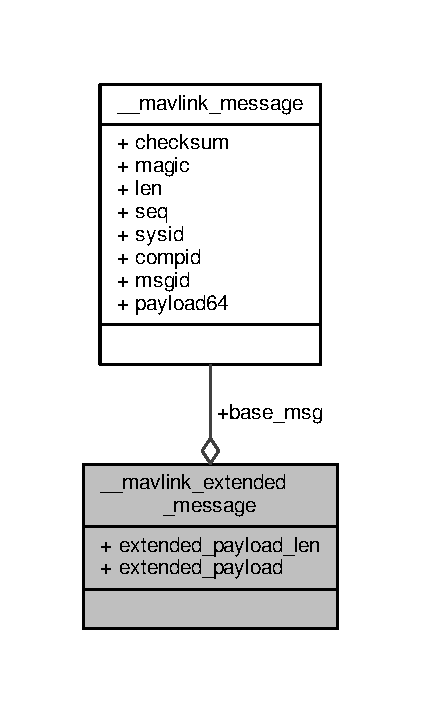
\includegraphics[width=202pt]{struct____mavlink__extended__message__coll__graph}
\end{center}
\end{figure}
\subsection*{Public Attributes}
\begin{DoxyCompactItemize}
\item 
\hypertarget{struct____mavlink__extended__message_a52d142dbcf71540bfc8199b45f676126}{\hyperlink{struct____mavlink__message}{mavlink\+\_\+message\+\_\+t} {\bfseries base\+\_\+msg}}\label{struct____mavlink__extended__message_a52d142dbcf71540bfc8199b45f676126}

\item 
\hypertarget{struct____mavlink__extended__message_a7fcf54d2c29dc157a78caacae8d998cf}{int32\+\_\+t \hyperlink{struct____mavlink__extended__message_a7fcf54d2c29dc157a78caacae8d998cf}{extended\+\_\+payload\+\_\+len}}\label{struct____mavlink__extended__message_a7fcf54d2c29dc157a78caacae8d998cf}

\begin{DoxyCompactList}\small\item\em Length of extended payload if any. \end{DoxyCompactList}\item 
\hypertarget{struct____mavlink__extended__message_afccf6dc3341050b0a63ac0d069d66a31}{uint8\+\_\+t {\bfseries extended\+\_\+payload} \mbox{[}M\+A\+V\+L\+I\+N\+K\+\_\+\+M\+A\+X\+\_\+\+E\+X\+T\+E\+N\+D\+E\+D\+\_\+\+P\+A\+Y\+L\+O\+A\+D\+\_\+\+L\+E\+N\mbox{]}}\label{struct____mavlink__extended__message_afccf6dc3341050b0a63ac0d069d66a31}

\end{DoxyCompactItemize}


The documentation for this struct was generated from the following file\+:\begin{DoxyCompactItemize}
\item 
/run/media/julien/\+Data/\+Documents/\+M\+A\+V\+R\+I\+C/\+M\+A\+V\+R\+I\+C\+\_\+\+Library/mavlink/include/mavlink\+\_\+types.\+h\end{DoxyCompactItemize}

\hypertarget{struct____mavlink__field__info}{\section{\+\_\+\+\_\+mavlink\+\_\+field\+\_\+info Struct Reference}
\label{struct____mavlink__field__info}\index{\+\_\+\+\_\+mavlink\+\_\+field\+\_\+info@{\+\_\+\+\_\+mavlink\+\_\+field\+\_\+info}}
}


Collaboration diagram for \+\_\+\+\_\+mavlink\+\_\+field\+\_\+info\+:
\nopagebreak
\begin{figure}[H]
\begin{center}
\leavevmode
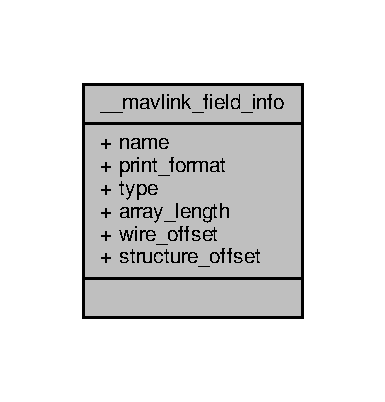
\includegraphics[width=185pt]{struct____mavlink__field__info__coll__graph}
\end{center}
\end{figure}
\subsection*{Public Attributes}
\begin{DoxyCompactItemize}
\item 
\hypertarget{struct____mavlink__field__info_a09193c7acc510180ecf6f944381e53c2}{const char $\ast$ {\bfseries name}}\label{struct____mavlink__field__info_a09193c7acc510180ecf6f944381e53c2}

\item 
\hypertarget{struct____mavlink__field__info_af3fc635b6e03851bb683c0c3d57dfc12}{const char $\ast$ {\bfseries print\+\_\+format}}\label{struct____mavlink__field__info_af3fc635b6e03851bb683c0c3d57dfc12}

\item 
\hypertarget{struct____mavlink__field__info_a32f98e7c869ae1567c4ad366c74b6552}{mavlink\+\_\+message\+\_\+type\+\_\+t {\bfseries type}}\label{struct____mavlink__field__info_a32f98e7c869ae1567c4ad366c74b6552}

\item 
\hypertarget{struct____mavlink__field__info_aa3ab268c4176743874c8d05694ed293f}{unsigned int {\bfseries array\+\_\+length}}\label{struct____mavlink__field__info_aa3ab268c4176743874c8d05694ed293f}

\item 
\hypertarget{struct____mavlink__field__info_a7156648575e497f112fde78e851dd4d9}{unsigned int {\bfseries wire\+\_\+offset}}\label{struct____mavlink__field__info_a7156648575e497f112fde78e851dd4d9}

\item 
\hypertarget{struct____mavlink__field__info_acb947cd22e51e70e8b5f677b543196ac}{unsigned int {\bfseries structure\+\_\+offset}}\label{struct____mavlink__field__info_acb947cd22e51e70e8b5f677b543196ac}

\end{DoxyCompactItemize}


The documentation for this struct was generated from the following file\+:\begin{DoxyCompactItemize}
\item 
/run/media/julien/\+Data/\+Documents/\+M\+A\+V\+R\+I\+C/\+M\+A\+V\+R\+I\+C\+\_\+\+Library/mavlink/include/mavlink\+\_\+types.\+h\end{DoxyCompactItemize}

\hypertarget{struct____mavlink__file__transfer__dir__list__t}{\section{\+\_\+\+\_\+mavlink\+\_\+file\+\_\+transfer\+\_\+dir\+\_\+list\+\_\+t Struct Reference}
\label{struct____mavlink__file__transfer__dir__list__t}\index{\+\_\+\+\_\+mavlink\+\_\+file\+\_\+transfer\+\_\+dir\+\_\+list\+\_\+t@{\+\_\+\+\_\+mavlink\+\_\+file\+\_\+transfer\+\_\+dir\+\_\+list\+\_\+t}}
}


Collaboration diagram for \+\_\+\+\_\+mavlink\+\_\+file\+\_\+transfer\+\_\+dir\+\_\+list\+\_\+t\+:
\nopagebreak
\begin{figure}[H]
\begin{center}
\leavevmode
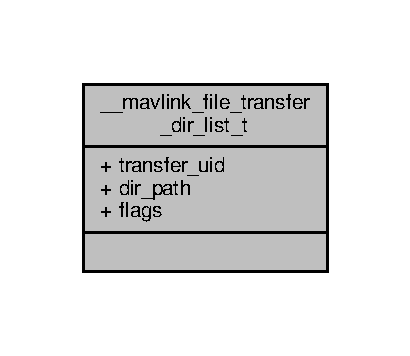
\includegraphics[width=197pt]{struct____mavlink__file__transfer__dir__list__t__coll__graph}
\end{center}
\end{figure}
\subsection*{Public Attributes}
\begin{DoxyCompactItemize}
\item 
\hypertarget{struct____mavlink__file__transfer__dir__list__t_ae4cbacc008aa59f7a6911f4723d0bc4c}{uint64\+\_\+t \hyperlink{struct____mavlink__file__transfer__dir__list__t_ae4cbacc008aa59f7a6911f4723d0bc4c}{transfer\+\_\+uid}}\label{struct____mavlink__file__transfer__dir__list__t_ae4cbacc008aa59f7a6911f4723d0bc4c}

\begin{DoxyCompactList}\small\item\em Unique transfer I\+D. \end{DoxyCompactList}\item 
\hypertarget{struct____mavlink__file__transfer__dir__list__t_aba9009fc7a7460bc54292796740ce9e3}{char \hyperlink{struct____mavlink__file__transfer__dir__list__t_aba9009fc7a7460bc54292796740ce9e3}{dir\+\_\+path} \mbox{[}240\mbox{]}}\label{struct____mavlink__file__transfer__dir__list__t_aba9009fc7a7460bc54292796740ce9e3}

\begin{DoxyCompactList}\small\item\em Directory path to list. \end{DoxyCompactList}\item 
\hypertarget{struct____mavlink__file__transfer__dir__list__t_a4f9a35692a267921d35fbace8507b581}{uint8\+\_\+t \hyperlink{struct____mavlink__file__transfer__dir__list__t_a4f9a35692a267921d35fbace8507b581}{flags}}\label{struct____mavlink__file__transfer__dir__list__t_a4f9a35692a267921d35fbace8507b581}

\begin{DoxyCompactList}\small\item\em R\+E\+S\+E\+R\+V\+E\+D. \end{DoxyCompactList}\end{DoxyCompactItemize}


The documentation for this struct was generated from the following file\+:\begin{DoxyCompactItemize}
\item 
/run/media/julien/\+Data/\+Documents/\+M\+A\+V\+R\+I\+C/\+M\+A\+V\+R\+I\+C\+\_\+\+Library/mavlink/include/common/mavlink\+\_\+msg\+\_\+file\+\_\+transfer\+\_\+dir\+\_\+list.\+h\end{DoxyCompactItemize}

\hypertarget{struct____mavlink__file__transfer__res__t}{\section{\+\_\+\+\_\+mavlink\+\_\+file\+\_\+transfer\+\_\+res\+\_\+t Struct Reference}
\label{struct____mavlink__file__transfer__res__t}\index{\+\_\+\+\_\+mavlink\+\_\+file\+\_\+transfer\+\_\+res\+\_\+t@{\+\_\+\+\_\+mavlink\+\_\+file\+\_\+transfer\+\_\+res\+\_\+t}}
}


Collaboration diagram for \+\_\+\+\_\+mavlink\+\_\+file\+\_\+transfer\+\_\+res\+\_\+t\+:
\nopagebreak
\begin{figure}[H]
\begin{center}
\leavevmode
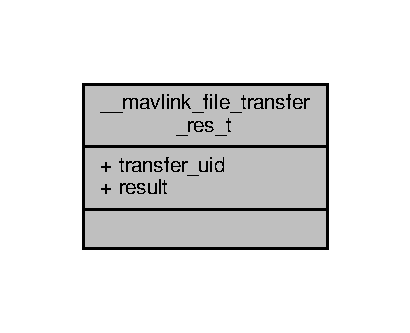
\includegraphics[width=197pt]{struct____mavlink__file__transfer__res__t__coll__graph}
\end{center}
\end{figure}
\subsection*{Public Attributes}
\begin{DoxyCompactItemize}
\item 
\hypertarget{struct____mavlink__file__transfer__res__t_ad8bbb4a8938103052075ed7f83b86eb8}{uint64\+\_\+t \hyperlink{struct____mavlink__file__transfer__res__t_ad8bbb4a8938103052075ed7f83b86eb8}{transfer\+\_\+uid}}\label{struct____mavlink__file__transfer__res__t_ad8bbb4a8938103052075ed7f83b86eb8}

\begin{DoxyCompactList}\small\item\em Unique transfer I\+D. \end{DoxyCompactList}\item 
\hypertarget{struct____mavlink__file__transfer__res__t_aac039b656fe7911fa9452bff8e9540b5}{uint8\+\_\+t \hyperlink{struct____mavlink__file__transfer__res__t_aac039b656fe7911fa9452bff8e9540b5}{result}}\label{struct____mavlink__file__transfer__res__t_aac039b656fe7911fa9452bff8e9540b5}

\begin{DoxyCompactList}\small\item\em 0\+: O\+K, 1\+: not permitted, 2\+: bad path / file name, 3\+: no space left on device \end{DoxyCompactList}\end{DoxyCompactItemize}


The documentation for this struct was generated from the following file\+:\begin{DoxyCompactItemize}
\item 
/run/media/julien/\+Data/\+Documents/\+M\+A\+V\+R\+I\+C/\+M\+A\+V\+R\+I\+C\+\_\+\+Library/mavlink/include/common/mavlink\+\_\+msg\+\_\+file\+\_\+transfer\+\_\+res.\+h\end{DoxyCompactItemize}

\hypertarget{struct____mavlink__file__transfer__start__t}{\section{\+\_\+\+\_\+mavlink\+\_\+file\+\_\+transfer\+\_\+start\+\_\+t Struct Reference}
\label{struct____mavlink__file__transfer__start__t}\index{\+\_\+\+\_\+mavlink\+\_\+file\+\_\+transfer\+\_\+start\+\_\+t@{\+\_\+\+\_\+mavlink\+\_\+file\+\_\+transfer\+\_\+start\+\_\+t}}
}


Collaboration diagram for \+\_\+\+\_\+mavlink\+\_\+file\+\_\+transfer\+\_\+start\+\_\+t\+:
\nopagebreak
\begin{figure}[H]
\begin{center}
\leavevmode
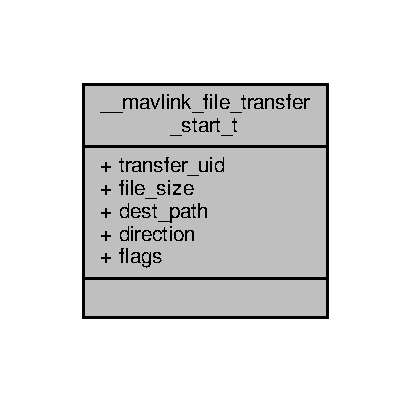
\includegraphics[width=197pt]{struct____mavlink__file__transfer__start__t__coll__graph}
\end{center}
\end{figure}
\subsection*{Public Attributes}
\begin{DoxyCompactItemize}
\item 
\hypertarget{struct____mavlink__file__transfer__start__t_a7c0e14ae134e2c92f6e7f688076bac3d}{uint64\+\_\+t \hyperlink{struct____mavlink__file__transfer__start__t_a7c0e14ae134e2c92f6e7f688076bac3d}{transfer\+\_\+uid}}\label{struct____mavlink__file__transfer__start__t_a7c0e14ae134e2c92f6e7f688076bac3d}

\begin{DoxyCompactList}\small\item\em Unique transfer I\+D. \end{DoxyCompactList}\item 
\hypertarget{struct____mavlink__file__transfer__start__t_a4bea17bbd0067dc18ac515c29be14bbe}{uint32\+\_\+t \hyperlink{struct____mavlink__file__transfer__start__t_a4bea17bbd0067dc18ac515c29be14bbe}{file\+\_\+size}}\label{struct____mavlink__file__transfer__start__t_a4bea17bbd0067dc18ac515c29be14bbe}

\begin{DoxyCompactList}\small\item\em File size in bytes. \end{DoxyCompactList}\item 
\hypertarget{struct____mavlink__file__transfer__start__t_ad6e81340d374e8fa65a8bb7a9f3f6602}{char \hyperlink{struct____mavlink__file__transfer__start__t_ad6e81340d374e8fa65a8bb7a9f3f6602}{dest\+\_\+path} \mbox{[}240\mbox{]}}\label{struct____mavlink__file__transfer__start__t_ad6e81340d374e8fa65a8bb7a9f3f6602}

\begin{DoxyCompactList}\small\item\em Destination path. \end{DoxyCompactList}\item 
\hypertarget{struct____mavlink__file__transfer__start__t_a28d4f521802039ee5b22607b578c6d65}{uint8\+\_\+t \hyperlink{struct____mavlink__file__transfer__start__t_a28d4f521802039ee5b22607b578c6d65}{direction}}\label{struct____mavlink__file__transfer__start__t_a28d4f521802039ee5b22607b578c6d65}

\begin{DoxyCompactList}\small\item\em Transfer direction\+: 0\+: from requester, 1\+: to requester. \end{DoxyCompactList}\item 
\hypertarget{struct____mavlink__file__transfer__start__t_aaeefe499ca015700989b21a6e9533935}{uint8\+\_\+t \hyperlink{struct____mavlink__file__transfer__start__t_aaeefe499ca015700989b21a6e9533935}{flags}}\label{struct____mavlink__file__transfer__start__t_aaeefe499ca015700989b21a6e9533935}

\begin{DoxyCompactList}\small\item\em R\+E\+S\+E\+R\+V\+E\+D. \end{DoxyCompactList}\end{DoxyCompactItemize}


The documentation for this struct was generated from the following file\+:\begin{DoxyCompactItemize}
\item 
/run/media/julien/\+Data/\+Documents/\+M\+A\+V\+R\+I\+C/\+M\+A\+V\+R\+I\+C\+\_\+\+Library/mavlink/include/common/mavlink\+\_\+msg\+\_\+file\+\_\+transfer\+\_\+start.\+h\end{DoxyCompactItemize}

\hypertarget{struct____mavlink__global__position__int__t}{\section{\+\_\+\+\_\+mavlink\+\_\+global\+\_\+position\+\_\+int\+\_\+t Struct Reference}
\label{struct____mavlink__global__position__int__t}\index{\+\_\+\+\_\+mavlink\+\_\+global\+\_\+position\+\_\+int\+\_\+t@{\+\_\+\+\_\+mavlink\+\_\+global\+\_\+position\+\_\+int\+\_\+t}}
}


Collaboration diagram for \+\_\+\+\_\+mavlink\+\_\+global\+\_\+position\+\_\+int\+\_\+t\+:
\nopagebreak
\begin{figure}[H]
\begin{center}
\leavevmode
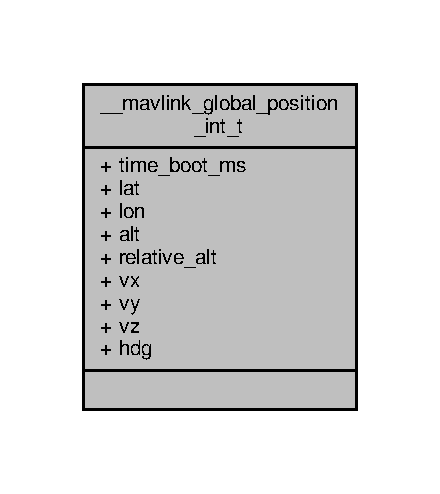
\includegraphics[width=211pt]{struct____mavlink__global__position__int__t__coll__graph}
\end{center}
\end{figure}
\subsection*{Public Attributes}
\begin{DoxyCompactItemize}
\item 
\hypertarget{struct____mavlink__global__position__int__t_a1b56c431f19cff6fadc2b0ac3b5959b6}{uint32\+\_\+t \hyperlink{struct____mavlink__global__position__int__t_a1b56c431f19cff6fadc2b0ac3b5959b6}{time\+\_\+boot\+\_\+ms}}\label{struct____mavlink__global__position__int__t_a1b56c431f19cff6fadc2b0ac3b5959b6}

\begin{DoxyCompactList}\small\item\em Timestamp (milliseconds since system boot) \end{DoxyCompactList}\item 
\hypertarget{struct____mavlink__global__position__int__t_a949653d08153161bb49b94794169a70f}{int32\+\_\+t \hyperlink{struct____mavlink__global__position__int__t_a949653d08153161bb49b94794169a70f}{lat}}\label{struct____mavlink__global__position__int__t_a949653d08153161bb49b94794169a70f}

\begin{DoxyCompactList}\small\item\em Latitude, expressed as $\ast$ 1\+E7. \end{DoxyCompactList}\item 
\hypertarget{struct____mavlink__global__position__int__t_a2350bdf8af429bc2ed49b7cfac61cee7}{int32\+\_\+t \hyperlink{struct____mavlink__global__position__int__t_a2350bdf8af429bc2ed49b7cfac61cee7}{lon}}\label{struct____mavlink__global__position__int__t_a2350bdf8af429bc2ed49b7cfac61cee7}

\begin{DoxyCompactList}\small\item\em Longitude, expressed as $\ast$ 1\+E7. \end{DoxyCompactList}\item 
\hypertarget{struct____mavlink__global__position__int__t_a1d9e69a26dc214bd624c9474ca3d79f4}{int32\+\_\+t \hyperlink{struct____mavlink__global__position__int__t_a1d9e69a26dc214bd624c9474ca3d79f4}{alt}}\label{struct____mavlink__global__position__int__t_a1d9e69a26dc214bd624c9474ca3d79f4}

\begin{DoxyCompactList}\small\item\em Altitude in meters, expressed as $\ast$ 1000 (millimeters), above M\+S\+L. \end{DoxyCompactList}\item 
\hypertarget{struct____mavlink__global__position__int__t_a1b3d36234adcacbedc88c37c1712f4b1}{int32\+\_\+t \hyperlink{struct____mavlink__global__position__int__t_a1b3d36234adcacbedc88c37c1712f4b1}{relative\+\_\+alt}}\label{struct____mavlink__global__position__int__t_a1b3d36234adcacbedc88c37c1712f4b1}

\begin{DoxyCompactList}\small\item\em Altitude above ground in meters, expressed as $\ast$ 1000 (millimeters) \end{DoxyCompactList}\item 
\hypertarget{struct____mavlink__global__position__int__t_a1f2bef1206e578e3f0f85f7854621829}{int16\+\_\+t \hyperlink{struct____mavlink__global__position__int__t_a1f2bef1206e578e3f0f85f7854621829}{vx}}\label{struct____mavlink__global__position__int__t_a1f2bef1206e578e3f0f85f7854621829}

\begin{DoxyCompactList}\small\item\em Ground X Speed (Latitude), expressed as m/s $\ast$ 100. \end{DoxyCompactList}\item 
\hypertarget{struct____mavlink__global__position__int__t_a89734a8b924f059f9e634233ce021cd3}{int16\+\_\+t \hyperlink{struct____mavlink__global__position__int__t_a89734a8b924f059f9e634233ce021cd3}{vy}}\label{struct____mavlink__global__position__int__t_a89734a8b924f059f9e634233ce021cd3}

\begin{DoxyCompactList}\small\item\em Ground Y Speed (Longitude), expressed as m/s $\ast$ 100. \end{DoxyCompactList}\item 
\hypertarget{struct____mavlink__global__position__int__t_ac476cea996cb642f139a93fc7f5ed2a4}{int16\+\_\+t \hyperlink{struct____mavlink__global__position__int__t_ac476cea996cb642f139a93fc7f5ed2a4}{vz}}\label{struct____mavlink__global__position__int__t_ac476cea996cb642f139a93fc7f5ed2a4}

\begin{DoxyCompactList}\small\item\em Ground Z Speed (Altitude), expressed as m/s $\ast$ 100. \end{DoxyCompactList}\item 
uint16\+\_\+t \hyperlink{struct____mavlink__global__position__int__t_a60f7c02018c444cdffb6121dee854e19}{hdg}
\begin{DoxyCompactList}\small\item\em Compass heading in degrees $\ast$ 100, 0.\+0..359.\+99 degrees. If unknown, set to\+: 65535. \end{DoxyCompactList}\end{DoxyCompactItemize}


\subsection{Member Data Documentation}
\hypertarget{struct____mavlink__global__position__int__t_a60f7c02018c444cdffb6121dee854e19}{\index{\+\_\+\+\_\+mavlink\+\_\+global\+\_\+position\+\_\+int\+\_\+t@{\+\_\+\+\_\+mavlink\+\_\+global\+\_\+position\+\_\+int\+\_\+t}!hdg@{hdg}}
\index{hdg@{hdg}!\+\_\+\+\_\+mavlink\+\_\+global\+\_\+position\+\_\+int\+\_\+t@{\+\_\+\+\_\+mavlink\+\_\+global\+\_\+position\+\_\+int\+\_\+t}}
\subsubsection[{hdg}]{\setlength{\rightskip}{0pt plus 5cm}uint16\+\_\+t \+\_\+\+\_\+mavlink\+\_\+global\+\_\+position\+\_\+int\+\_\+t\+::hdg}}\label{struct____mavlink__global__position__int__t_a60f7c02018c444cdffb6121dee854e19}


Compass heading in degrees $\ast$ 100, 0.\+0..359.\+99 degrees. If unknown, set to\+: 65535. 

Compass heading in degrees $\ast$ 100, 0.\+0..359.\+99 degrees. If unknown, set to\+: U\+I\+N\+T16\+\_\+\+M\+A\+X. 

The documentation for this struct was generated from the following file\+:\begin{DoxyCompactItemize}
\item 
/run/media/julien/\+Data/\+Documents/\+M\+A\+V\+R\+I\+C/\+M\+A\+V\+R\+I\+C\+\_\+\+Library/mavlink/include/common/mavlink\+\_\+msg\+\_\+global\+\_\+position\+\_\+int.\+h\end{DoxyCompactItemize}

\hypertarget{struct____mavlink__global__position__setpoint__int__t}{\section{\+\_\+\+\_\+mavlink\+\_\+global\+\_\+position\+\_\+setpoint\+\_\+int\+\_\+t Struct Reference}
\label{struct____mavlink__global__position__setpoint__int__t}\index{\+\_\+\+\_\+mavlink\+\_\+global\+\_\+position\+\_\+setpoint\+\_\+int\+\_\+t@{\+\_\+\+\_\+mavlink\+\_\+global\+\_\+position\+\_\+setpoint\+\_\+int\+\_\+t}}
}


Collaboration diagram for \+\_\+\+\_\+mavlink\+\_\+global\+\_\+position\+\_\+setpoint\+\_\+int\+\_\+t\+:
\nopagebreak
\begin{figure}[H]
\begin{center}
\leavevmode
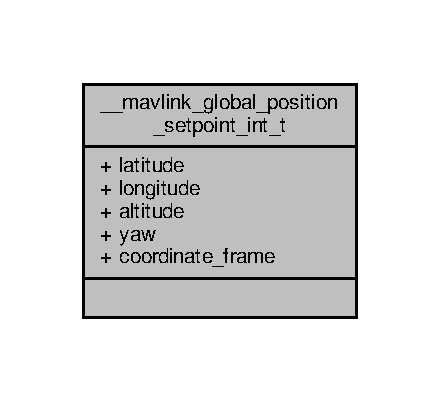
\includegraphics[width=211pt]{struct____mavlink__global__position__setpoint__int__t__coll__graph}
\end{center}
\end{figure}
\subsection*{Public Attributes}
\begin{DoxyCompactItemize}
\item 
int32\+\_\+t \hyperlink{struct____mavlink__global__position__setpoint__int__t_a7b02635b701aa77624372077915df167}{latitude}
\begin{DoxyCompactList}\small\item\em W\+G\+S84 Latitude position in degrees $\ast$ 1\+E7. \end{DoxyCompactList}\item 
int32\+\_\+t \hyperlink{struct____mavlink__global__position__setpoint__int__t_a290bd746e9d22250d7a9396afbc8a8b9}{longitude}
\begin{DoxyCompactList}\small\item\em W\+G\+S84 Longitude position in degrees $\ast$ 1\+E7. \end{DoxyCompactList}\item 
int32\+\_\+t \hyperlink{struct____mavlink__global__position__setpoint__int__t_a73aa1270e7a36b8b86857221366b5a4d}{altitude}
\begin{DoxyCompactList}\small\item\em W\+G\+S84 Altitude in meters $\ast$ 1000 (positive for up) \end{DoxyCompactList}\item 
\hypertarget{struct____mavlink__global__position__setpoint__int__t_ab4e559ebe301ccdb64580e34febf2d86}{int16\+\_\+t \hyperlink{struct____mavlink__global__position__setpoint__int__t_ab4e559ebe301ccdb64580e34febf2d86}{yaw}}\label{struct____mavlink__global__position__setpoint__int__t_ab4e559ebe301ccdb64580e34febf2d86}

\begin{DoxyCompactList}\small\item\em Desired yaw angle in degrees $\ast$ 100. \end{DoxyCompactList}\item 
\hypertarget{struct____mavlink__global__position__setpoint__int__t_aca893671888c2856ff4e8d67a267d3ac}{uint8\+\_\+t \hyperlink{struct____mavlink__global__position__setpoint__int__t_aca893671888c2856ff4e8d67a267d3ac}{coordinate\+\_\+frame}}\label{struct____mavlink__global__position__setpoint__int__t_aca893671888c2856ff4e8d67a267d3ac}

\begin{DoxyCompactList}\small\item\em Coordinate frame -\/ valid values are only M\+A\+V\+\_\+\+F\+R\+A\+M\+E\+\_\+\+G\+L\+O\+B\+A\+L or M\+A\+V\+\_\+\+F\+R\+A\+M\+E\+\_\+\+G\+L\+O\+B\+A\+L\+\_\+\+R\+E\+L\+A\+T\+I\+V\+E\+\_\+\+A\+L\+T. \end{DoxyCompactList}\end{DoxyCompactItemize}


\subsection{Member Data Documentation}
\hypertarget{struct____mavlink__global__position__setpoint__int__t_a73aa1270e7a36b8b86857221366b5a4d}{\index{\+\_\+\+\_\+mavlink\+\_\+global\+\_\+position\+\_\+setpoint\+\_\+int\+\_\+t@{\+\_\+\+\_\+mavlink\+\_\+global\+\_\+position\+\_\+setpoint\+\_\+int\+\_\+t}!altitude@{altitude}}
\index{altitude@{altitude}!\+\_\+\+\_\+mavlink\+\_\+global\+\_\+position\+\_\+setpoint\+\_\+int\+\_\+t@{\+\_\+\+\_\+mavlink\+\_\+global\+\_\+position\+\_\+setpoint\+\_\+int\+\_\+t}}
\subsubsection[{altitude}]{\setlength{\rightskip}{0pt plus 5cm}int32\+\_\+t \+\_\+\+\_\+mavlink\+\_\+global\+\_\+position\+\_\+setpoint\+\_\+int\+\_\+t\+::altitude}}\label{struct____mavlink__global__position__setpoint__int__t_a73aa1270e7a36b8b86857221366b5a4d}


W\+G\+S84 Altitude in meters $\ast$ 1000 (positive for up) 

Altitude (W\+G\+S84), in meters $\ast$ 1000 (positive for up) \hypertarget{struct____mavlink__global__position__setpoint__int__t_a7b02635b701aa77624372077915df167}{\index{\+\_\+\+\_\+mavlink\+\_\+global\+\_\+position\+\_\+setpoint\+\_\+int\+\_\+t@{\+\_\+\+\_\+mavlink\+\_\+global\+\_\+position\+\_\+setpoint\+\_\+int\+\_\+t}!latitude@{latitude}}
\index{latitude@{latitude}!\+\_\+\+\_\+mavlink\+\_\+global\+\_\+position\+\_\+setpoint\+\_\+int\+\_\+t@{\+\_\+\+\_\+mavlink\+\_\+global\+\_\+position\+\_\+setpoint\+\_\+int\+\_\+t}}
\subsubsection[{latitude}]{\setlength{\rightskip}{0pt plus 5cm}int32\+\_\+t \+\_\+\+\_\+mavlink\+\_\+global\+\_\+position\+\_\+setpoint\+\_\+int\+\_\+t\+::latitude}}\label{struct____mavlink__global__position__setpoint__int__t_a7b02635b701aa77624372077915df167}


W\+G\+S84 Latitude position in degrees $\ast$ 1\+E7. 

Latitude (W\+G\+S84), in degrees $\ast$ 1\+E7. \hypertarget{struct____mavlink__global__position__setpoint__int__t_a290bd746e9d22250d7a9396afbc8a8b9}{\index{\+\_\+\+\_\+mavlink\+\_\+global\+\_\+position\+\_\+setpoint\+\_\+int\+\_\+t@{\+\_\+\+\_\+mavlink\+\_\+global\+\_\+position\+\_\+setpoint\+\_\+int\+\_\+t}!longitude@{longitude}}
\index{longitude@{longitude}!\+\_\+\+\_\+mavlink\+\_\+global\+\_\+position\+\_\+setpoint\+\_\+int\+\_\+t@{\+\_\+\+\_\+mavlink\+\_\+global\+\_\+position\+\_\+setpoint\+\_\+int\+\_\+t}}
\subsubsection[{longitude}]{\setlength{\rightskip}{0pt plus 5cm}int32\+\_\+t \+\_\+\+\_\+mavlink\+\_\+global\+\_\+position\+\_\+setpoint\+\_\+int\+\_\+t\+::longitude}}\label{struct____mavlink__global__position__setpoint__int__t_a290bd746e9d22250d7a9396afbc8a8b9}


W\+G\+S84 Longitude position in degrees $\ast$ 1\+E7. 

Longitude (W\+G\+S84), in degrees $\ast$ 1\+E7. 

The documentation for this struct was generated from the following file\+:\begin{DoxyCompactItemize}
\item 
/run/media/julien/\+Data/\+Documents/\+M\+A\+V\+R\+I\+C/\+M\+A\+V\+R\+I\+C\+\_\+\+Library/mavlink/include/common/mavlink\+\_\+msg\+\_\+global\+\_\+position\+\_\+setpoint\+\_\+int.\+h\end{DoxyCompactItemize}

\hypertarget{struct____mavlink__global__vision__position__estimate__t}{\section{\+\_\+\+\_\+mavlink\+\_\+global\+\_\+vision\+\_\+position\+\_\+estimate\+\_\+t Struct Reference}
\label{struct____mavlink__global__vision__position__estimate__t}\index{\+\_\+\+\_\+mavlink\+\_\+global\+\_\+vision\+\_\+position\+\_\+estimate\+\_\+t@{\+\_\+\+\_\+mavlink\+\_\+global\+\_\+vision\+\_\+position\+\_\+estimate\+\_\+t}}
}


Collaboration diagram for \+\_\+\+\_\+mavlink\+\_\+global\+\_\+vision\+\_\+position\+\_\+estimate\+\_\+t\+:
\nopagebreak
\begin{figure}[H]
\begin{center}
\leavevmode
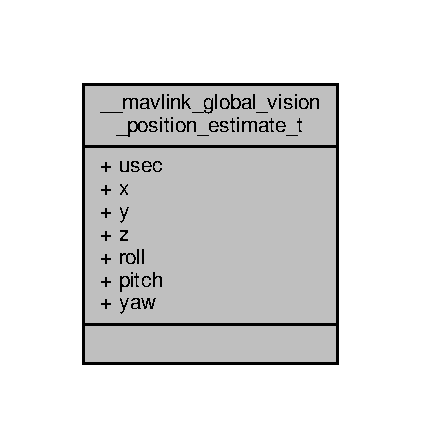
\includegraphics[width=202pt]{struct____mavlink__global__vision__position__estimate__t__coll__graph}
\end{center}
\end{figure}
\subsection*{Public Attributes}
\begin{DoxyCompactItemize}
\item 
\hypertarget{struct____mavlink__global__vision__position__estimate__t_acf639462e3875daf642a84fc1a1a829b}{uint64\+\_\+t \hyperlink{struct____mavlink__global__vision__position__estimate__t_acf639462e3875daf642a84fc1a1a829b}{usec}}\label{struct____mavlink__global__vision__position__estimate__t_acf639462e3875daf642a84fc1a1a829b}

\begin{DoxyCompactList}\small\item\em Timestamp (microseconds, synced to U\+N\+I\+X time or since system boot) \end{DoxyCompactList}\item 
\hypertarget{struct____mavlink__global__vision__position__estimate__t_a88cd56fff31fdbd1490526e27e56811a}{float \hyperlink{struct____mavlink__global__vision__position__estimate__t_a88cd56fff31fdbd1490526e27e56811a}{x}}\label{struct____mavlink__global__vision__position__estimate__t_a88cd56fff31fdbd1490526e27e56811a}

\begin{DoxyCompactList}\small\item\em Global X position. \end{DoxyCompactList}\item 
\hypertarget{struct____mavlink__global__vision__position__estimate__t_a8d9936412bbccb077e7cd7c608ff4293}{float \hyperlink{struct____mavlink__global__vision__position__estimate__t_a8d9936412bbccb077e7cd7c608ff4293}{y}}\label{struct____mavlink__global__vision__position__estimate__t_a8d9936412bbccb077e7cd7c608ff4293}

\begin{DoxyCompactList}\small\item\em Global Y position. \end{DoxyCompactList}\item 
\hypertarget{struct____mavlink__global__vision__position__estimate__t_ab7cb6c5e88d406ac8566580d0c4003ee}{float \hyperlink{struct____mavlink__global__vision__position__estimate__t_ab7cb6c5e88d406ac8566580d0c4003ee}{z}}\label{struct____mavlink__global__vision__position__estimate__t_ab7cb6c5e88d406ac8566580d0c4003ee}

\begin{DoxyCompactList}\small\item\em Global Z position. \end{DoxyCompactList}\item 
\hypertarget{struct____mavlink__global__vision__position__estimate__t_a1cbae0267ad81e4c6ac223c433ee5941}{float \hyperlink{struct____mavlink__global__vision__position__estimate__t_a1cbae0267ad81e4c6ac223c433ee5941}{roll}}\label{struct____mavlink__global__vision__position__estimate__t_a1cbae0267ad81e4c6ac223c433ee5941}

\begin{DoxyCompactList}\small\item\em Roll angle in rad. \end{DoxyCompactList}\item 
\hypertarget{struct____mavlink__global__vision__position__estimate__t_ac36453fff07f0620a7c81c5eb31d8ce4}{float \hyperlink{struct____mavlink__global__vision__position__estimate__t_ac36453fff07f0620a7c81c5eb31d8ce4}{pitch}}\label{struct____mavlink__global__vision__position__estimate__t_ac36453fff07f0620a7c81c5eb31d8ce4}

\begin{DoxyCompactList}\small\item\em Pitch angle in rad. \end{DoxyCompactList}\item 
\hypertarget{struct____mavlink__global__vision__position__estimate__t_adcbed99801fc5b5e77817e56c9e74cce}{float \hyperlink{struct____mavlink__global__vision__position__estimate__t_adcbed99801fc5b5e77817e56c9e74cce}{yaw}}\label{struct____mavlink__global__vision__position__estimate__t_adcbed99801fc5b5e77817e56c9e74cce}

\begin{DoxyCompactList}\small\item\em Yaw angle in rad. \end{DoxyCompactList}\end{DoxyCompactItemize}


The documentation for this struct was generated from the following file\+:\begin{DoxyCompactItemize}
\item 
/run/media/julien/\+Data/\+Documents/\+M\+A\+V\+R\+I\+C/\+M\+A\+V\+R\+I\+C\+\_\+\+Library/mavlink/include/common/mavlink\+\_\+msg\+\_\+global\+\_\+vision\+\_\+position\+\_\+estimate.\+h\end{DoxyCompactItemize}

\hypertarget{struct____mavlink__gps__global__origin__t}{\section{\+\_\+\+\_\+mavlink\+\_\+gps\+\_\+global\+\_\+origin\+\_\+t Struct Reference}
\label{struct____mavlink__gps__global__origin__t}\index{\+\_\+\+\_\+mavlink\+\_\+gps\+\_\+global\+\_\+origin\+\_\+t@{\+\_\+\+\_\+mavlink\+\_\+gps\+\_\+global\+\_\+origin\+\_\+t}}
}


Collaboration diagram for \+\_\+\+\_\+mavlink\+\_\+gps\+\_\+global\+\_\+origin\+\_\+t\+:
\nopagebreak
\begin{figure}[H]
\begin{center}
\leavevmode
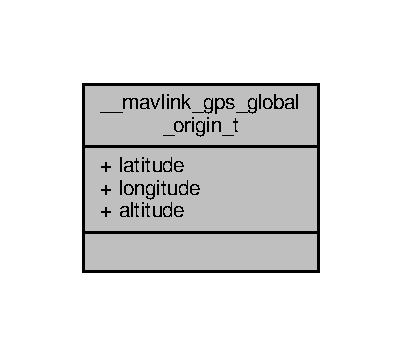
\includegraphics[width=193pt]{struct____mavlink__gps__global__origin__t__coll__graph}
\end{center}
\end{figure}
\subsection*{Public Attributes}
\begin{DoxyCompactItemize}
\item 
int32\+\_\+t \hyperlink{struct____mavlink__gps__global__origin__t_ab78807fb15062419bf5452c3294235bc}{latitude}
\begin{DoxyCompactList}\small\item\em Latitude (W\+G\+S84), expressed as $\ast$ 1\+E7. \end{DoxyCompactList}\item 
int32\+\_\+t \hyperlink{struct____mavlink__gps__global__origin__t_a52156dc446e0be0bc5cbf4247e194349}{longitude}
\begin{DoxyCompactList}\small\item\em Longitude (W\+G\+S84), expressed as $\ast$ 1\+E7. \end{DoxyCompactList}\item 
int32\+\_\+t \hyperlink{struct____mavlink__gps__global__origin__t_a34577699f6c0ef2517eb8b16da733c15}{altitude}
\begin{DoxyCompactList}\small\item\em Altitude(\+W\+G\+S84), expressed as $\ast$ 1000. \end{DoxyCompactList}\end{DoxyCompactItemize}


\subsection{Member Data Documentation}
\hypertarget{struct____mavlink__gps__global__origin__t_a34577699f6c0ef2517eb8b16da733c15}{\index{\+\_\+\+\_\+mavlink\+\_\+gps\+\_\+global\+\_\+origin\+\_\+t@{\+\_\+\+\_\+mavlink\+\_\+gps\+\_\+global\+\_\+origin\+\_\+t}!altitude@{altitude}}
\index{altitude@{altitude}!\+\_\+\+\_\+mavlink\+\_\+gps\+\_\+global\+\_\+origin\+\_\+t@{\+\_\+\+\_\+mavlink\+\_\+gps\+\_\+global\+\_\+origin\+\_\+t}}
\subsubsection[{altitude}]{\setlength{\rightskip}{0pt plus 5cm}int32\+\_\+t \+\_\+\+\_\+mavlink\+\_\+gps\+\_\+global\+\_\+origin\+\_\+t\+::altitude}}\label{struct____mavlink__gps__global__origin__t_a34577699f6c0ef2517eb8b16da733c15}


Altitude(\+W\+G\+S84), expressed as $\ast$ 1000. 

Altitude (W\+G\+S84), in meters $\ast$ 1000 (positive for up) \hypertarget{struct____mavlink__gps__global__origin__t_ab78807fb15062419bf5452c3294235bc}{\index{\+\_\+\+\_\+mavlink\+\_\+gps\+\_\+global\+\_\+origin\+\_\+t@{\+\_\+\+\_\+mavlink\+\_\+gps\+\_\+global\+\_\+origin\+\_\+t}!latitude@{latitude}}
\index{latitude@{latitude}!\+\_\+\+\_\+mavlink\+\_\+gps\+\_\+global\+\_\+origin\+\_\+t@{\+\_\+\+\_\+mavlink\+\_\+gps\+\_\+global\+\_\+origin\+\_\+t}}
\subsubsection[{latitude}]{\setlength{\rightskip}{0pt plus 5cm}int32\+\_\+t \+\_\+\+\_\+mavlink\+\_\+gps\+\_\+global\+\_\+origin\+\_\+t\+::latitude}}\label{struct____mavlink__gps__global__origin__t_ab78807fb15062419bf5452c3294235bc}


Latitude (W\+G\+S84), expressed as $\ast$ 1\+E7. 

Latitude (W\+G\+S84), in degrees $\ast$ 1\+E7. \hypertarget{struct____mavlink__gps__global__origin__t_a52156dc446e0be0bc5cbf4247e194349}{\index{\+\_\+\+\_\+mavlink\+\_\+gps\+\_\+global\+\_\+origin\+\_\+t@{\+\_\+\+\_\+mavlink\+\_\+gps\+\_\+global\+\_\+origin\+\_\+t}!longitude@{longitude}}
\index{longitude@{longitude}!\+\_\+\+\_\+mavlink\+\_\+gps\+\_\+global\+\_\+origin\+\_\+t@{\+\_\+\+\_\+mavlink\+\_\+gps\+\_\+global\+\_\+origin\+\_\+t}}
\subsubsection[{longitude}]{\setlength{\rightskip}{0pt plus 5cm}int32\+\_\+t \+\_\+\+\_\+mavlink\+\_\+gps\+\_\+global\+\_\+origin\+\_\+t\+::longitude}}\label{struct____mavlink__gps__global__origin__t_a52156dc446e0be0bc5cbf4247e194349}


Longitude (W\+G\+S84), expressed as $\ast$ 1\+E7. 

Longitude (W\+G\+S84), in degrees $\ast$ 1\+E7. 

The documentation for this struct was generated from the following file\+:\begin{DoxyCompactItemize}
\item 
/run/media/julien/\+Data/\+Documents/\+M\+A\+V\+R\+I\+C/\+M\+A\+V\+R\+I\+C\+\_\+\+Library/mavlink/include/common/mavlink\+\_\+msg\+\_\+gps\+\_\+global\+\_\+origin.\+h\end{DoxyCompactItemize}

\hypertarget{struct____mavlink__gps__raw__int__t}{\section{\+\_\+\+\_\+mavlink\+\_\+gps\+\_\+raw\+\_\+int\+\_\+t Struct Reference}
\label{struct____mavlink__gps__raw__int__t}\index{\+\_\+\+\_\+mavlink\+\_\+gps\+\_\+raw\+\_\+int\+\_\+t@{\+\_\+\+\_\+mavlink\+\_\+gps\+\_\+raw\+\_\+int\+\_\+t}}
}


Collaboration diagram for \+\_\+\+\_\+mavlink\+\_\+gps\+\_\+raw\+\_\+int\+\_\+t\+:
\nopagebreak
\begin{figure}[H]
\begin{center}
\leavevmode
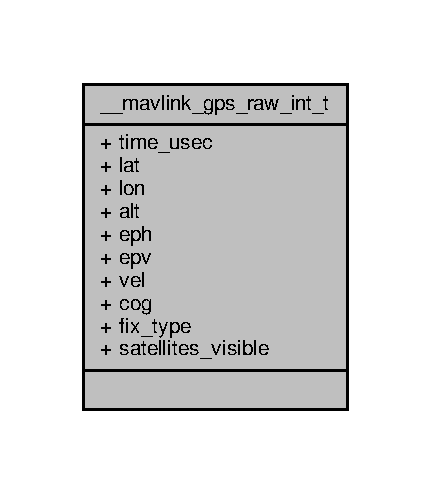
\includegraphics[width=207pt]{struct____mavlink__gps__raw__int__t__coll__graph}
\end{center}
\end{figure}
\subsection*{Public Attributes}
\begin{DoxyCompactItemize}
\item 
\hypertarget{struct____mavlink__gps__raw__int__t_a39d30393d02f2b1882040e3fa063f6ea}{uint64\+\_\+t \hyperlink{struct____mavlink__gps__raw__int__t_a39d30393d02f2b1882040e3fa063f6ea}{time\+\_\+usec}}\label{struct____mavlink__gps__raw__int__t_a39d30393d02f2b1882040e3fa063f6ea}

\begin{DoxyCompactList}\small\item\em Timestamp (microseconds since U\+N\+I\+X epoch or microseconds since system boot) \end{DoxyCompactList}\item 
int32\+\_\+t \hyperlink{struct____mavlink__gps__raw__int__t_aefd27d0b2d23c58a59b218aa151220d3}{lat}
\begin{DoxyCompactList}\small\item\em Latitude in 1\+E7 degrees. \end{DoxyCompactList}\item 
int32\+\_\+t \hyperlink{struct____mavlink__gps__raw__int__t_a025fd2dd700ff7180af5a26c2a3497f4}{lon}
\begin{DoxyCompactList}\small\item\em Longitude in 1\+E7 degrees. \end{DoxyCompactList}\item 
int32\+\_\+t \hyperlink{struct____mavlink__gps__raw__int__t_a00fe92144cfdaf8440a841493e5b6e99}{alt}
\begin{DoxyCompactList}\small\item\em Altitude in 1\+E3 meters (millimeters) above M\+S\+L. \end{DoxyCompactList}\item 
uint16\+\_\+t \hyperlink{struct____mavlink__gps__raw__int__t_ad7ec0749ffe37d3ada65b701be2cd305}{eph}
\begin{DoxyCompactList}\small\item\em G\+P\+S H\+D\+O\+P horizontal dilution of position in cm (m$\ast$100). If unknown, set to\+: 65535. \end{DoxyCompactList}\item 
uint16\+\_\+t \hyperlink{struct____mavlink__gps__raw__int__t_a0d50bc6cc0e56d9f49885e3e550ec944}{epv}
\begin{DoxyCompactList}\small\item\em G\+P\+S V\+D\+O\+P horizontal dilution of position in cm (m$\ast$100). If unknown, set to\+: 65535. \end{DoxyCompactList}\item 
uint16\+\_\+t \hyperlink{struct____mavlink__gps__raw__int__t_a77e8cbdbf554637e4fbbdaaabd562eaf}{vel}
\begin{DoxyCompactList}\small\item\em G\+P\+S ground speed (m/s $\ast$ 100). If unknown, set to\+: 65535. \end{DoxyCompactList}\item 
uint16\+\_\+t \hyperlink{struct____mavlink__gps__raw__int__t_adbe4dfbea17d1fd08a0841ce29e32637}{cog}
\begin{DoxyCompactList}\small\item\em Course over ground (N\+O\+T heading, but direction of movement) in degrees $\ast$ 100, 0.\+0..359.\+99 degrees. If unknown, set to\+: 65535. \end{DoxyCompactList}\item 
\hypertarget{struct____mavlink__gps__raw__int__t_ae014afb6eea2b6033ebde37c79e120f2}{uint8\+\_\+t \hyperlink{struct____mavlink__gps__raw__int__t_ae014afb6eea2b6033ebde37c79e120f2}{fix\+\_\+type}}\label{struct____mavlink__gps__raw__int__t_ae014afb6eea2b6033ebde37c79e120f2}

\begin{DoxyCompactList}\small\item\em 0-\/1\+: no fix, 2\+: 2\+D fix, 3\+: 3\+D fix. Some applications will not use the value of this field unless it is at least two, so always correctly fill in the fix. \end{DoxyCompactList}\item 
\hypertarget{struct____mavlink__gps__raw__int__t_af1481a191aa3ffbf832dc3a4c35cbf09}{uint8\+\_\+t \hyperlink{struct____mavlink__gps__raw__int__t_af1481a191aa3ffbf832dc3a4c35cbf09}{satellites\+\_\+visible}}\label{struct____mavlink__gps__raw__int__t_af1481a191aa3ffbf832dc3a4c35cbf09}

\begin{DoxyCompactList}\small\item\em Number of satellites visible. If unknown, set to 255. \end{DoxyCompactList}\end{DoxyCompactItemize}


\subsection{Member Data Documentation}
\hypertarget{struct____mavlink__gps__raw__int__t_a00fe92144cfdaf8440a841493e5b6e99}{\index{\+\_\+\+\_\+mavlink\+\_\+gps\+\_\+raw\+\_\+int\+\_\+t@{\+\_\+\+\_\+mavlink\+\_\+gps\+\_\+raw\+\_\+int\+\_\+t}!alt@{alt}}
\index{alt@{alt}!\+\_\+\+\_\+mavlink\+\_\+gps\+\_\+raw\+\_\+int\+\_\+t@{\+\_\+\+\_\+mavlink\+\_\+gps\+\_\+raw\+\_\+int\+\_\+t}}
\subsubsection[{alt}]{\setlength{\rightskip}{0pt plus 5cm}int32\+\_\+t \+\_\+\+\_\+mavlink\+\_\+gps\+\_\+raw\+\_\+int\+\_\+t\+::alt}}\label{struct____mavlink__gps__raw__int__t_a00fe92144cfdaf8440a841493e5b6e99}


Altitude in 1\+E3 meters (millimeters) above M\+S\+L. 

Altitude (W\+G\+S84), in meters $\ast$ 1000 (positive for up) \hypertarget{struct____mavlink__gps__raw__int__t_adbe4dfbea17d1fd08a0841ce29e32637}{\index{\+\_\+\+\_\+mavlink\+\_\+gps\+\_\+raw\+\_\+int\+\_\+t@{\+\_\+\+\_\+mavlink\+\_\+gps\+\_\+raw\+\_\+int\+\_\+t}!cog@{cog}}
\index{cog@{cog}!\+\_\+\+\_\+mavlink\+\_\+gps\+\_\+raw\+\_\+int\+\_\+t@{\+\_\+\+\_\+mavlink\+\_\+gps\+\_\+raw\+\_\+int\+\_\+t}}
\subsubsection[{cog}]{\setlength{\rightskip}{0pt plus 5cm}uint16\+\_\+t \+\_\+\+\_\+mavlink\+\_\+gps\+\_\+raw\+\_\+int\+\_\+t\+::cog}}\label{struct____mavlink__gps__raw__int__t_adbe4dfbea17d1fd08a0841ce29e32637}


Course over ground (N\+O\+T heading, but direction of movement) in degrees $\ast$ 100, 0.\+0..359.\+99 degrees. If unknown, set to\+: 65535. 

Course over ground (N\+O\+T heading, but direction of movement) in degrees $\ast$ 100, 0.\+0..359.\+99 degrees. If unknown, set to\+: U\+I\+N\+T16\+\_\+\+M\+A\+X. \hypertarget{struct____mavlink__gps__raw__int__t_ad7ec0749ffe37d3ada65b701be2cd305}{\index{\+\_\+\+\_\+mavlink\+\_\+gps\+\_\+raw\+\_\+int\+\_\+t@{\+\_\+\+\_\+mavlink\+\_\+gps\+\_\+raw\+\_\+int\+\_\+t}!eph@{eph}}
\index{eph@{eph}!\+\_\+\+\_\+mavlink\+\_\+gps\+\_\+raw\+\_\+int\+\_\+t@{\+\_\+\+\_\+mavlink\+\_\+gps\+\_\+raw\+\_\+int\+\_\+t}}
\subsubsection[{eph}]{\setlength{\rightskip}{0pt plus 5cm}uint16\+\_\+t \+\_\+\+\_\+mavlink\+\_\+gps\+\_\+raw\+\_\+int\+\_\+t\+::eph}}\label{struct____mavlink__gps__raw__int__t_ad7ec0749ffe37d3ada65b701be2cd305}


G\+P\+S H\+D\+O\+P horizontal dilution of position in cm (m$\ast$100). If unknown, set to\+: 65535. 

G\+P\+S H\+D\+O\+P horizontal dilution of position in cm (m$\ast$100). If unknown, set to\+: U\+I\+N\+T16\+\_\+\+M\+A\+X. \hypertarget{struct____mavlink__gps__raw__int__t_a0d50bc6cc0e56d9f49885e3e550ec944}{\index{\+\_\+\+\_\+mavlink\+\_\+gps\+\_\+raw\+\_\+int\+\_\+t@{\+\_\+\+\_\+mavlink\+\_\+gps\+\_\+raw\+\_\+int\+\_\+t}!epv@{epv}}
\index{epv@{epv}!\+\_\+\+\_\+mavlink\+\_\+gps\+\_\+raw\+\_\+int\+\_\+t@{\+\_\+\+\_\+mavlink\+\_\+gps\+\_\+raw\+\_\+int\+\_\+t}}
\subsubsection[{epv}]{\setlength{\rightskip}{0pt plus 5cm}uint16\+\_\+t \+\_\+\+\_\+mavlink\+\_\+gps\+\_\+raw\+\_\+int\+\_\+t\+::epv}}\label{struct____mavlink__gps__raw__int__t_a0d50bc6cc0e56d9f49885e3e550ec944}


G\+P\+S V\+D\+O\+P horizontal dilution of position in cm (m$\ast$100). If unknown, set to\+: 65535. 

G\+P\+S V\+D\+O\+P horizontal dilution of position in cm (m$\ast$100). If unknown, set to\+: U\+I\+N\+T16\+\_\+\+M\+A\+X. \hypertarget{struct____mavlink__gps__raw__int__t_aefd27d0b2d23c58a59b218aa151220d3}{\index{\+\_\+\+\_\+mavlink\+\_\+gps\+\_\+raw\+\_\+int\+\_\+t@{\+\_\+\+\_\+mavlink\+\_\+gps\+\_\+raw\+\_\+int\+\_\+t}!lat@{lat}}
\index{lat@{lat}!\+\_\+\+\_\+mavlink\+\_\+gps\+\_\+raw\+\_\+int\+\_\+t@{\+\_\+\+\_\+mavlink\+\_\+gps\+\_\+raw\+\_\+int\+\_\+t}}
\subsubsection[{lat}]{\setlength{\rightskip}{0pt plus 5cm}int32\+\_\+t \+\_\+\+\_\+mavlink\+\_\+gps\+\_\+raw\+\_\+int\+\_\+t\+::lat}}\label{struct____mavlink__gps__raw__int__t_aefd27d0b2d23c58a59b218aa151220d3}


Latitude in 1\+E7 degrees. 

Latitude (W\+G\+S84), in degrees $\ast$ 1\+E7. \hypertarget{struct____mavlink__gps__raw__int__t_a025fd2dd700ff7180af5a26c2a3497f4}{\index{\+\_\+\+\_\+mavlink\+\_\+gps\+\_\+raw\+\_\+int\+\_\+t@{\+\_\+\+\_\+mavlink\+\_\+gps\+\_\+raw\+\_\+int\+\_\+t}!lon@{lon}}
\index{lon@{lon}!\+\_\+\+\_\+mavlink\+\_\+gps\+\_\+raw\+\_\+int\+\_\+t@{\+\_\+\+\_\+mavlink\+\_\+gps\+\_\+raw\+\_\+int\+\_\+t}}
\subsubsection[{lon}]{\setlength{\rightskip}{0pt plus 5cm}int32\+\_\+t \+\_\+\+\_\+mavlink\+\_\+gps\+\_\+raw\+\_\+int\+\_\+t\+::lon}}\label{struct____mavlink__gps__raw__int__t_a025fd2dd700ff7180af5a26c2a3497f4}


Longitude in 1\+E7 degrees. 

Longitude (W\+G\+S84), in degrees $\ast$ 1\+E7. \hypertarget{struct____mavlink__gps__raw__int__t_a77e8cbdbf554637e4fbbdaaabd562eaf}{\index{\+\_\+\+\_\+mavlink\+\_\+gps\+\_\+raw\+\_\+int\+\_\+t@{\+\_\+\+\_\+mavlink\+\_\+gps\+\_\+raw\+\_\+int\+\_\+t}!vel@{vel}}
\index{vel@{vel}!\+\_\+\+\_\+mavlink\+\_\+gps\+\_\+raw\+\_\+int\+\_\+t@{\+\_\+\+\_\+mavlink\+\_\+gps\+\_\+raw\+\_\+int\+\_\+t}}
\subsubsection[{vel}]{\setlength{\rightskip}{0pt plus 5cm}uint16\+\_\+t \+\_\+\+\_\+mavlink\+\_\+gps\+\_\+raw\+\_\+int\+\_\+t\+::vel}}\label{struct____mavlink__gps__raw__int__t_a77e8cbdbf554637e4fbbdaaabd562eaf}


G\+P\+S ground speed (m/s $\ast$ 100). If unknown, set to\+: 65535. 

G\+P\+S ground speed (m/s $\ast$ 100). If unknown, set to\+: U\+I\+N\+T16\+\_\+\+M\+A\+X. 

The documentation for this struct was generated from the following file\+:\begin{DoxyCompactItemize}
\item 
/run/media/julien/\+Data/\+Documents/\+M\+A\+V\+R\+I\+C/\+M\+A\+V\+R\+I\+C\+\_\+\+Library/mavlink/include/common/mavlink\+\_\+msg\+\_\+gps\+\_\+raw\+\_\+int.\+h\end{DoxyCompactItemize}

\hypertarget{struct____mavlink__gps__status__t}{\section{\+\_\+\+\_\+mavlink\+\_\+gps\+\_\+status\+\_\+t Struct Reference}
\label{struct____mavlink__gps__status__t}\index{\+\_\+\+\_\+mavlink\+\_\+gps\+\_\+status\+\_\+t@{\+\_\+\+\_\+mavlink\+\_\+gps\+\_\+status\+\_\+t}}
}


Collaboration diagram for \+\_\+\+\_\+mavlink\+\_\+gps\+\_\+status\+\_\+t\+:
\nopagebreak
\begin{figure}[H]
\begin{center}
\leavevmode
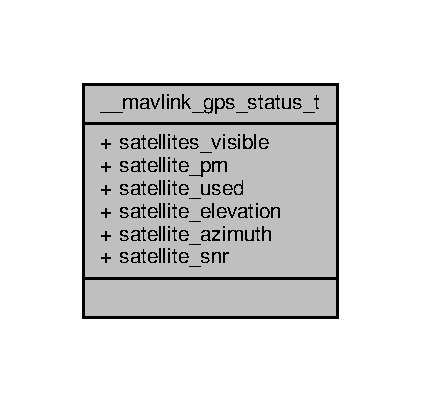
\includegraphics[width=202pt]{struct____mavlink__gps__status__t__coll__graph}
\end{center}
\end{figure}
\subsection*{Public Attributes}
\begin{DoxyCompactItemize}
\item 
\hypertarget{struct____mavlink__gps__status__t_aaf907a0b7ca1bf692b59b3c07269a72d}{uint8\+\_\+t \hyperlink{struct____mavlink__gps__status__t_aaf907a0b7ca1bf692b59b3c07269a72d}{satellites\+\_\+visible}}\label{struct____mavlink__gps__status__t_aaf907a0b7ca1bf692b59b3c07269a72d}

\begin{DoxyCompactList}\small\item\em Number of satellites visible. \end{DoxyCompactList}\item 
\hypertarget{struct____mavlink__gps__status__t_ab95bb265fee555d17a40a25b53c5fa40}{uint8\+\_\+t \hyperlink{struct____mavlink__gps__status__t_ab95bb265fee555d17a40a25b53c5fa40}{satellite\+\_\+prn} \mbox{[}20\mbox{]}}\label{struct____mavlink__gps__status__t_ab95bb265fee555d17a40a25b53c5fa40}

\begin{DoxyCompactList}\small\item\em Global satellite I\+D. \end{DoxyCompactList}\item 
\hypertarget{struct____mavlink__gps__status__t_a4f563283322cfea1b77374cb7db283ff}{uint8\+\_\+t \hyperlink{struct____mavlink__gps__status__t_a4f563283322cfea1b77374cb7db283ff}{satellite\+\_\+used} \mbox{[}20\mbox{]}}\label{struct____mavlink__gps__status__t_a4f563283322cfea1b77374cb7db283ff}

\begin{DoxyCompactList}\small\item\em 0\+: Satellite not used, 1\+: used for localization \end{DoxyCompactList}\item 
\hypertarget{struct____mavlink__gps__status__t_a8513963d43bac3d30179680f24601ac5}{uint8\+\_\+t \hyperlink{struct____mavlink__gps__status__t_a8513963d43bac3d30179680f24601ac5}{satellite\+\_\+elevation} \mbox{[}20\mbox{]}}\label{struct____mavlink__gps__status__t_a8513963d43bac3d30179680f24601ac5}

\begin{DoxyCompactList}\small\item\em Elevation (0\+: right on top of receiver, 90\+: on the horizon) of satellite. \end{DoxyCompactList}\item 
\hypertarget{struct____mavlink__gps__status__t_aef5900af3f2a1431059a28ef6f8a9a70}{uint8\+\_\+t \hyperlink{struct____mavlink__gps__status__t_aef5900af3f2a1431059a28ef6f8a9a70}{satellite\+\_\+azimuth} \mbox{[}20\mbox{]}}\label{struct____mavlink__gps__status__t_aef5900af3f2a1431059a28ef6f8a9a70}

\begin{DoxyCompactList}\small\item\em Direction of satellite, 0\+: 0 deg, 255\+: 360 deg. \end{DoxyCompactList}\item 
\hypertarget{struct____mavlink__gps__status__t_af5c2ca556c0063e74f387849118d9f33}{uint8\+\_\+t \hyperlink{struct____mavlink__gps__status__t_af5c2ca556c0063e74f387849118d9f33}{satellite\+\_\+snr} \mbox{[}20\mbox{]}}\label{struct____mavlink__gps__status__t_af5c2ca556c0063e74f387849118d9f33}

\begin{DoxyCompactList}\small\item\em Signal to noise ratio of satellite. \end{DoxyCompactList}\end{DoxyCompactItemize}


The documentation for this struct was generated from the following file\+:\begin{DoxyCompactItemize}
\item 
/run/media/julien/\+Data/\+Documents/\+M\+A\+V\+R\+I\+C/\+M\+A\+V\+R\+I\+C\+\_\+\+Library/mavlink/include/common/mavlink\+\_\+msg\+\_\+gps\+\_\+status.\+h\end{DoxyCompactItemize}

\hypertarget{struct____mavlink__heartbeat__t}{\section{\+\_\+\+\_\+mavlink\+\_\+heartbeat\+\_\+t Struct Reference}
\label{struct____mavlink__heartbeat__t}\index{\+\_\+\+\_\+mavlink\+\_\+heartbeat\+\_\+t@{\+\_\+\+\_\+mavlink\+\_\+heartbeat\+\_\+t}}
}


Collaboration diagram for \+\_\+\+\_\+mavlink\+\_\+heartbeat\+\_\+t\+:
\nopagebreak
\begin{figure}[H]
\begin{center}
\leavevmode
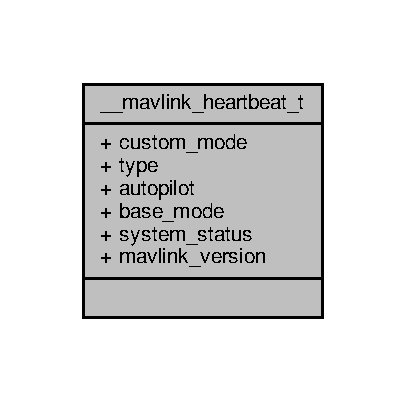
\includegraphics[width=195pt]{struct____mavlink__heartbeat__t__coll__graph}
\end{center}
\end{figure}
\subsection*{Public Attributes}
\begin{DoxyCompactItemize}
\item 
\hypertarget{struct____mavlink__heartbeat__t_a4d8e5d4a59f775887eaecfd58303e17d}{uint32\+\_\+t \hyperlink{struct____mavlink__heartbeat__t_a4d8e5d4a59f775887eaecfd58303e17d}{custom\+\_\+mode}}\label{struct____mavlink__heartbeat__t_a4d8e5d4a59f775887eaecfd58303e17d}

\begin{DoxyCompactList}\small\item\em A bitfield for use for autopilot-\/specific flags. \end{DoxyCompactList}\item 
\hypertarget{struct____mavlink__heartbeat__t_a2f34a5f641022acd59d9b54e69976341}{uint8\+\_\+t \hyperlink{struct____mavlink__heartbeat__t_a2f34a5f641022acd59d9b54e69976341}{type}}\label{struct____mavlink__heartbeat__t_a2f34a5f641022acd59d9b54e69976341}

\begin{DoxyCompactList}\small\item\em Type of the M\+A\+V (quadrotor, helicopter, etc., up to 15 types, defined in M\+A\+V\+\_\+\+T\+Y\+P\+E E\+N\+U\+M) \end{DoxyCompactList}\item 
\hypertarget{struct____mavlink__heartbeat__t_a5be04782d8a0bb715ad26c25cce74b9b}{uint8\+\_\+t \hyperlink{struct____mavlink__heartbeat__t_a5be04782d8a0bb715ad26c25cce74b9b}{autopilot}}\label{struct____mavlink__heartbeat__t_a5be04782d8a0bb715ad26c25cce74b9b}

\begin{DoxyCompactList}\small\item\em Autopilot type / class. defined in M\+A\+V\+\_\+\+A\+U\+T\+O\+P\+I\+L\+O\+T E\+N\+U\+M. \end{DoxyCompactList}\item 
\hypertarget{struct____mavlink__heartbeat__t_a816ec38dcbb0f4948185efbdd96ebb5e}{uint8\+\_\+t \hyperlink{struct____mavlink__heartbeat__t_a816ec38dcbb0f4948185efbdd96ebb5e}{base\+\_\+mode}}\label{struct____mavlink__heartbeat__t_a816ec38dcbb0f4948185efbdd96ebb5e}

\begin{DoxyCompactList}\small\item\em System mode bitfield, see M\+A\+V\+\_\+\+M\+O\+D\+E\+\_\+\+F\+L\+A\+G\+S E\+N\+U\+M in \hyperlink{mavlink__types_8h_source}{mavlink/include/mavlink\+\_\+types.\+h}. \end{DoxyCompactList}\item 
\hypertarget{struct____mavlink__heartbeat__t_a914b772577c4898cc5bfe4ece1c8529d}{uint8\+\_\+t \hyperlink{struct____mavlink__heartbeat__t_a914b772577c4898cc5bfe4ece1c8529d}{system\+\_\+status}}\label{struct____mavlink__heartbeat__t_a914b772577c4898cc5bfe4ece1c8529d}

\begin{DoxyCompactList}\small\item\em System status flag, see M\+A\+V\+\_\+\+S\+T\+A\+T\+E E\+N\+U\+M. \end{DoxyCompactList}\item 
\hypertarget{struct____mavlink__heartbeat__t_a235d5b6a09fa9b24b3ef7b7a28d15b97}{uint8\+\_\+t \hyperlink{struct____mavlink__heartbeat__t_a235d5b6a09fa9b24b3ef7b7a28d15b97}{mavlink\+\_\+version}}\label{struct____mavlink__heartbeat__t_a235d5b6a09fa9b24b3ef7b7a28d15b97}

\begin{DoxyCompactList}\small\item\em M\+A\+V\+Link version, not writable by user, gets added by protocol because of magic data type\+: uint8\+\_\+t\+\_\+mavlink\+\_\+version. \end{DoxyCompactList}\end{DoxyCompactItemize}


The documentation for this struct was generated from the following file\+:\begin{DoxyCompactItemize}
\item 
/run/media/julien/\+Data/\+Documents/\+M\+A\+V\+R\+I\+C/\+M\+A\+V\+R\+I\+C\+\_\+\+Library/mavlink/include/common/mavlink\+\_\+msg\+\_\+heartbeat.\+h\end{DoxyCompactItemize}

\hypertarget{struct____mavlink__highres__imu__t}{\section{\+\_\+\+\_\+mavlink\+\_\+highres\+\_\+imu\+\_\+t Struct Reference}
\label{struct____mavlink__highres__imu__t}\index{\+\_\+\+\_\+mavlink\+\_\+highres\+\_\+imu\+\_\+t@{\+\_\+\+\_\+mavlink\+\_\+highres\+\_\+imu\+\_\+t}}
}


Collaboration diagram for \+\_\+\+\_\+mavlink\+\_\+highres\+\_\+imu\+\_\+t\+:
\nopagebreak
\begin{figure}[H]
\begin{center}
\leavevmode
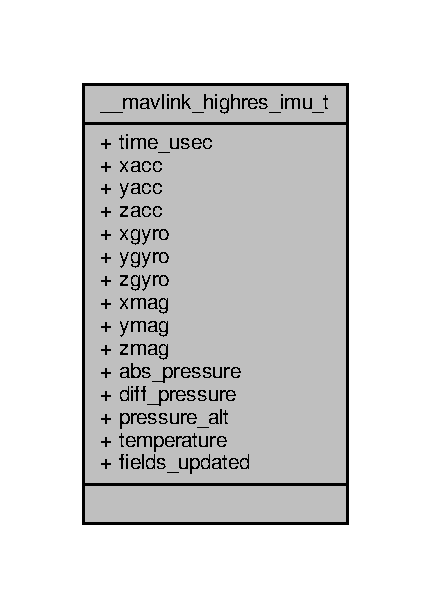
\includegraphics[width=207pt]{struct____mavlink__highres__imu__t__coll__graph}
\end{center}
\end{figure}
\subsection*{Public Attributes}
\begin{DoxyCompactItemize}
\item 
\hypertarget{struct____mavlink__highres__imu__t_aaf1a08b7dcf5ed9ca8ce6f66c392d678}{uint64\+\_\+t \hyperlink{struct____mavlink__highres__imu__t_aaf1a08b7dcf5ed9ca8ce6f66c392d678}{time\+\_\+usec}}\label{struct____mavlink__highres__imu__t_aaf1a08b7dcf5ed9ca8ce6f66c392d678}

\begin{DoxyCompactList}\small\item\em Timestamp (microseconds, synced to U\+N\+I\+X time or since system boot) \end{DoxyCompactList}\item 
\hypertarget{struct____mavlink__highres__imu__t_ace5e765b886ddee9ea50983177bea172}{float \hyperlink{struct____mavlink__highres__imu__t_ace5e765b886ddee9ea50983177bea172}{xacc}}\label{struct____mavlink__highres__imu__t_ace5e765b886ddee9ea50983177bea172}

\begin{DoxyCompactList}\small\item\em X acceleration (m/s$^\wedge$2) \end{DoxyCompactList}\item 
\hypertarget{struct____mavlink__highres__imu__t_aedf7c76d0487a09e980851fd6162ae17}{float \hyperlink{struct____mavlink__highres__imu__t_aedf7c76d0487a09e980851fd6162ae17}{yacc}}\label{struct____mavlink__highres__imu__t_aedf7c76d0487a09e980851fd6162ae17}

\begin{DoxyCompactList}\small\item\em Y acceleration (m/s$^\wedge$2) \end{DoxyCompactList}\item 
\hypertarget{struct____mavlink__highres__imu__t_a01f05eb6ed0c4b0db807f22bf6134ab4}{float \hyperlink{struct____mavlink__highres__imu__t_a01f05eb6ed0c4b0db807f22bf6134ab4}{zacc}}\label{struct____mavlink__highres__imu__t_a01f05eb6ed0c4b0db807f22bf6134ab4}

\begin{DoxyCompactList}\small\item\em Z acceleration (m/s$^\wedge$2) \end{DoxyCompactList}\item 
\hypertarget{struct____mavlink__highres__imu__t_ae736b5fdd1185a4ec6c2947d652778e1}{float \hyperlink{struct____mavlink__highres__imu__t_ae736b5fdd1185a4ec6c2947d652778e1}{xgyro}}\label{struct____mavlink__highres__imu__t_ae736b5fdd1185a4ec6c2947d652778e1}

\begin{DoxyCompactList}\small\item\em Angular speed around X axis (rad / sec) \end{DoxyCompactList}\item 
\hypertarget{struct____mavlink__highres__imu__t_a593f56b2ae4f9d85c8e9f8a06e28aef3}{float \hyperlink{struct____mavlink__highres__imu__t_a593f56b2ae4f9d85c8e9f8a06e28aef3}{ygyro}}\label{struct____mavlink__highres__imu__t_a593f56b2ae4f9d85c8e9f8a06e28aef3}

\begin{DoxyCompactList}\small\item\em Angular speed around Y axis (rad / sec) \end{DoxyCompactList}\item 
\hypertarget{struct____mavlink__highres__imu__t_a3e5d5462ef68fe4fea7811c082ddb186}{float \hyperlink{struct____mavlink__highres__imu__t_a3e5d5462ef68fe4fea7811c082ddb186}{zgyro}}\label{struct____mavlink__highres__imu__t_a3e5d5462ef68fe4fea7811c082ddb186}

\begin{DoxyCompactList}\small\item\em Angular speed around Z axis (rad / sec) \end{DoxyCompactList}\item 
\hypertarget{struct____mavlink__highres__imu__t_a82d9c25f53b9ee64f48c99f45eaead70}{float \hyperlink{struct____mavlink__highres__imu__t_a82d9c25f53b9ee64f48c99f45eaead70}{xmag}}\label{struct____mavlink__highres__imu__t_a82d9c25f53b9ee64f48c99f45eaead70}

\begin{DoxyCompactList}\small\item\em X Magnetic field (Gauss) \end{DoxyCompactList}\item 
\hypertarget{struct____mavlink__highres__imu__t_aa887e516e745fef0f051856c46b8e0f6}{float \hyperlink{struct____mavlink__highres__imu__t_aa887e516e745fef0f051856c46b8e0f6}{ymag}}\label{struct____mavlink__highres__imu__t_aa887e516e745fef0f051856c46b8e0f6}

\begin{DoxyCompactList}\small\item\em Y Magnetic field (Gauss) \end{DoxyCompactList}\item 
\hypertarget{struct____mavlink__highres__imu__t_abf5f119c9468cfaeb83d757997024a57}{float \hyperlink{struct____mavlink__highres__imu__t_abf5f119c9468cfaeb83d757997024a57}{zmag}}\label{struct____mavlink__highres__imu__t_abf5f119c9468cfaeb83d757997024a57}

\begin{DoxyCompactList}\small\item\em Z Magnetic field (Gauss) \end{DoxyCompactList}\item 
\hypertarget{struct____mavlink__highres__imu__t_a0db713a894b40a11ee5b0cddc1629353}{float \hyperlink{struct____mavlink__highres__imu__t_a0db713a894b40a11ee5b0cddc1629353}{abs\+\_\+pressure}}\label{struct____mavlink__highres__imu__t_a0db713a894b40a11ee5b0cddc1629353}

\begin{DoxyCompactList}\small\item\em Absolute pressure in millibar. \end{DoxyCompactList}\item 
\hypertarget{struct____mavlink__highres__imu__t_a5902061bb3028121e55ce9641e844334}{float \hyperlink{struct____mavlink__highres__imu__t_a5902061bb3028121e55ce9641e844334}{diff\+\_\+pressure}}\label{struct____mavlink__highres__imu__t_a5902061bb3028121e55ce9641e844334}

\begin{DoxyCompactList}\small\item\em Differential pressure in millibar. \end{DoxyCompactList}\item 
\hypertarget{struct____mavlink__highres__imu__t_ae540d0d0572455b1fc44123d3a3b6405}{float \hyperlink{struct____mavlink__highres__imu__t_ae540d0d0572455b1fc44123d3a3b6405}{pressure\+\_\+alt}}\label{struct____mavlink__highres__imu__t_ae540d0d0572455b1fc44123d3a3b6405}

\begin{DoxyCompactList}\small\item\em Altitude calculated from pressure. \end{DoxyCompactList}\item 
\hypertarget{struct____mavlink__highres__imu__t_add75673ef20a41e9548b3b583762d4b4}{float \hyperlink{struct____mavlink__highres__imu__t_add75673ef20a41e9548b3b583762d4b4}{temperature}}\label{struct____mavlink__highres__imu__t_add75673ef20a41e9548b3b583762d4b4}

\begin{DoxyCompactList}\small\item\em Temperature in degrees celsius. \end{DoxyCompactList}\item 
\hypertarget{struct____mavlink__highres__imu__t_a0723ff71a7057f3f96eb64ac73be64dc}{uint16\+\_\+t \hyperlink{struct____mavlink__highres__imu__t_a0723ff71a7057f3f96eb64ac73be64dc}{fields\+\_\+updated}}\label{struct____mavlink__highres__imu__t_a0723ff71a7057f3f96eb64ac73be64dc}

\begin{DoxyCompactList}\small\item\em Bitmask for fields that have updated since last message, bit 0 = xacc, bit 12\+: temperature. \end{DoxyCompactList}\end{DoxyCompactItemize}


The documentation for this struct was generated from the following file\+:\begin{DoxyCompactItemize}
\item 
/run/media/julien/\+Data/\+Documents/\+M\+A\+V\+R\+I\+C/\+M\+A\+V\+R\+I\+C\+\_\+\+Library/mavlink/include/common/mavlink\+\_\+msg\+\_\+highres\+\_\+imu.\+h\end{DoxyCompactItemize}

\hypertarget{struct____mavlink__hil__controls__t}{\section{\+\_\+\+\_\+mavlink\+\_\+hil\+\_\+controls\+\_\+t Struct Reference}
\label{struct____mavlink__hil__controls__t}\index{\+\_\+\+\_\+mavlink\+\_\+hil\+\_\+controls\+\_\+t@{\+\_\+\+\_\+mavlink\+\_\+hil\+\_\+controls\+\_\+t}}
}


Collaboration diagram for \+\_\+\+\_\+mavlink\+\_\+hil\+\_\+controls\+\_\+t\+:
\nopagebreak
\begin{figure}[H]
\begin{center}
\leavevmode
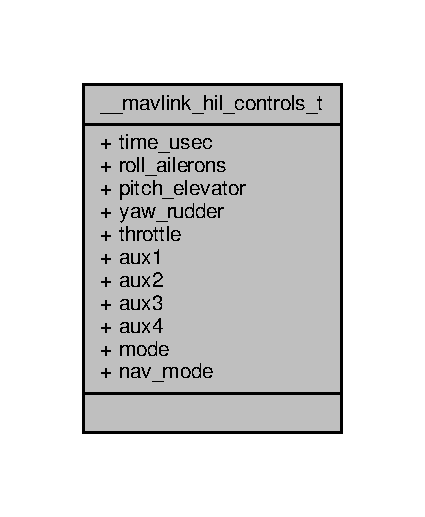
\includegraphics[width=204pt]{struct____mavlink__hil__controls__t__coll__graph}
\end{center}
\end{figure}
\subsection*{Public Attributes}
\begin{DoxyCompactItemize}
\item 
\hypertarget{struct____mavlink__hil__controls__t_a209e91b6d93c47abba3dc4ed3c6625f2}{uint64\+\_\+t \hyperlink{struct____mavlink__hil__controls__t_a209e91b6d93c47abba3dc4ed3c6625f2}{time\+\_\+usec}}\label{struct____mavlink__hil__controls__t_a209e91b6d93c47abba3dc4ed3c6625f2}

\begin{DoxyCompactList}\small\item\em Timestamp (microseconds since U\+N\+I\+X epoch or microseconds since system boot) \end{DoxyCompactList}\item 
\hypertarget{struct____mavlink__hil__controls__t_a65303ffed89e791c1551bf41d3d764dc}{float \hyperlink{struct____mavlink__hil__controls__t_a65303ffed89e791c1551bf41d3d764dc}{roll\+\_\+ailerons}}\label{struct____mavlink__hil__controls__t_a65303ffed89e791c1551bf41d3d764dc}

\begin{DoxyCompactList}\small\item\em Control output -\/1 .. 1. \end{DoxyCompactList}\item 
\hypertarget{struct____mavlink__hil__controls__t_ae1da8c6e2be5e9927f9748671d901764}{float \hyperlink{struct____mavlink__hil__controls__t_ae1da8c6e2be5e9927f9748671d901764}{pitch\+\_\+elevator}}\label{struct____mavlink__hil__controls__t_ae1da8c6e2be5e9927f9748671d901764}

\begin{DoxyCompactList}\small\item\em Control output -\/1 .. 1. \end{DoxyCompactList}\item 
\hypertarget{struct____mavlink__hil__controls__t_addcaf6167ddb280643e69558a0532dd8}{float \hyperlink{struct____mavlink__hil__controls__t_addcaf6167ddb280643e69558a0532dd8}{yaw\+\_\+rudder}}\label{struct____mavlink__hil__controls__t_addcaf6167ddb280643e69558a0532dd8}

\begin{DoxyCompactList}\small\item\em Control output -\/1 .. 1. \end{DoxyCompactList}\item 
\hypertarget{struct____mavlink__hil__controls__t_a9249963d6b4959b9cbc952ad86e2a2f1}{float \hyperlink{struct____mavlink__hil__controls__t_a9249963d6b4959b9cbc952ad86e2a2f1}{throttle}}\label{struct____mavlink__hil__controls__t_a9249963d6b4959b9cbc952ad86e2a2f1}

\begin{DoxyCompactList}\small\item\em Throttle 0 .. 1. \end{DoxyCompactList}\item 
\hypertarget{struct____mavlink__hil__controls__t_ae8a7a69971e009abc390ed6f1950936a}{float \hyperlink{struct____mavlink__hil__controls__t_ae8a7a69971e009abc390ed6f1950936a}{aux1}}\label{struct____mavlink__hil__controls__t_ae8a7a69971e009abc390ed6f1950936a}

\begin{DoxyCompactList}\small\item\em Aux 1, -\/1 .. 1. \end{DoxyCompactList}\item 
\hypertarget{struct____mavlink__hil__controls__t_a34ee57a5807ad445506db9ba666e13d1}{float \hyperlink{struct____mavlink__hil__controls__t_a34ee57a5807ad445506db9ba666e13d1}{aux2}}\label{struct____mavlink__hil__controls__t_a34ee57a5807ad445506db9ba666e13d1}

\begin{DoxyCompactList}\small\item\em Aux 2, -\/1 .. 1. \end{DoxyCompactList}\item 
\hypertarget{struct____mavlink__hil__controls__t_ac90aa43f5be0ad189f9e42a4afec883f}{float \hyperlink{struct____mavlink__hil__controls__t_ac90aa43f5be0ad189f9e42a4afec883f}{aux3}}\label{struct____mavlink__hil__controls__t_ac90aa43f5be0ad189f9e42a4afec883f}

\begin{DoxyCompactList}\small\item\em Aux 3, -\/1 .. 1. \end{DoxyCompactList}\item 
\hypertarget{struct____mavlink__hil__controls__t_a0b636589ba52581e9e7cde07f8f90e12}{float \hyperlink{struct____mavlink__hil__controls__t_a0b636589ba52581e9e7cde07f8f90e12}{aux4}}\label{struct____mavlink__hil__controls__t_a0b636589ba52581e9e7cde07f8f90e12}

\begin{DoxyCompactList}\small\item\em Aux 4, -\/1 .. 1. \end{DoxyCompactList}\item 
\hypertarget{struct____mavlink__hil__controls__t_a44828f146b2d8fa81c7da0e844a18e39}{uint8\+\_\+t \hyperlink{struct____mavlink__hil__controls__t_a44828f146b2d8fa81c7da0e844a18e39}{mode}}\label{struct____mavlink__hil__controls__t_a44828f146b2d8fa81c7da0e844a18e39}

\begin{DoxyCompactList}\small\item\em System mode (M\+A\+V\+\_\+\+M\+O\+D\+E) \end{DoxyCompactList}\item 
\hypertarget{struct____mavlink__hil__controls__t_adcc556cd52256501a39b1f9e962ca5b6}{uint8\+\_\+t \hyperlink{struct____mavlink__hil__controls__t_adcc556cd52256501a39b1f9e962ca5b6}{nav\+\_\+mode}}\label{struct____mavlink__hil__controls__t_adcc556cd52256501a39b1f9e962ca5b6}

\begin{DoxyCompactList}\small\item\em Navigation mode (M\+A\+V\+\_\+\+N\+A\+V\+\_\+\+M\+O\+D\+E) \end{DoxyCompactList}\end{DoxyCompactItemize}


The documentation for this struct was generated from the following file\+:\begin{DoxyCompactItemize}
\item 
/run/media/julien/\+Data/\+Documents/\+M\+A\+V\+R\+I\+C/\+M\+A\+V\+R\+I\+C\+\_\+\+Library/mavlink/include/common/mavlink\+\_\+msg\+\_\+hil\+\_\+controls.\+h\end{DoxyCompactItemize}

\hypertarget{struct____mavlink__hil__gps__t}{\section{\+\_\+\+\_\+mavlink\+\_\+hil\+\_\+gps\+\_\+t Struct Reference}
\label{struct____mavlink__hil__gps__t}\index{\+\_\+\+\_\+mavlink\+\_\+hil\+\_\+gps\+\_\+t@{\+\_\+\+\_\+mavlink\+\_\+hil\+\_\+gps\+\_\+t}}
}


Collaboration diagram for \+\_\+\+\_\+mavlink\+\_\+hil\+\_\+gps\+\_\+t\+:
\nopagebreak
\begin{figure}[H]
\begin{center}
\leavevmode
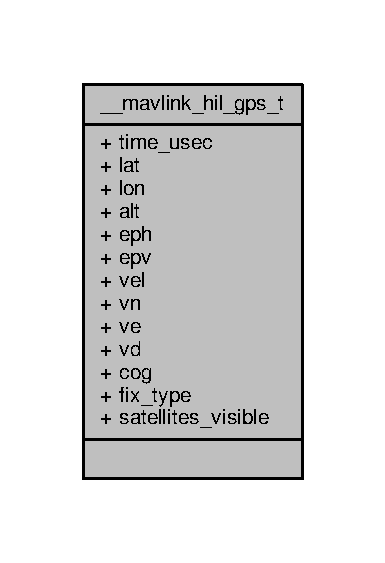
\includegraphics[width=185pt]{struct____mavlink__hil__gps__t__coll__graph}
\end{center}
\end{figure}
\subsection*{Public Attributes}
\begin{DoxyCompactItemize}
\item 
\hypertarget{struct____mavlink__hil__gps__t_a06069c8971366092665b51a939e9abb3}{uint64\+\_\+t \hyperlink{struct____mavlink__hil__gps__t_a06069c8971366092665b51a939e9abb3}{time\+\_\+usec}}\label{struct____mavlink__hil__gps__t_a06069c8971366092665b51a939e9abb3}

\begin{DoxyCompactList}\small\item\em Timestamp (microseconds since U\+N\+I\+X epoch or microseconds since system boot) \end{DoxyCompactList}\item 
\hypertarget{struct____mavlink__hil__gps__t_a5adc957f66ccbd23fe9bfabd056c03c5}{int32\+\_\+t \hyperlink{struct____mavlink__hil__gps__t_a5adc957f66ccbd23fe9bfabd056c03c5}{lat}}\label{struct____mavlink__hil__gps__t_a5adc957f66ccbd23fe9bfabd056c03c5}

\begin{DoxyCompactList}\small\item\em Latitude (W\+G\+S84), in degrees $\ast$ 1\+E7. \end{DoxyCompactList}\item 
\hypertarget{struct____mavlink__hil__gps__t_abfec6d143d48f5b7e5e37cd8c98d6f82}{int32\+\_\+t \hyperlink{struct____mavlink__hil__gps__t_abfec6d143d48f5b7e5e37cd8c98d6f82}{lon}}\label{struct____mavlink__hil__gps__t_abfec6d143d48f5b7e5e37cd8c98d6f82}

\begin{DoxyCompactList}\small\item\em Longitude (W\+G\+S84), in degrees $\ast$ 1\+E7. \end{DoxyCompactList}\item 
\hypertarget{struct____mavlink__hil__gps__t_a9d9f5ccc1ded23c02b7a7ed760c66a73}{int32\+\_\+t \hyperlink{struct____mavlink__hil__gps__t_a9d9f5ccc1ded23c02b7a7ed760c66a73}{alt}}\label{struct____mavlink__hil__gps__t_a9d9f5ccc1ded23c02b7a7ed760c66a73}

\begin{DoxyCompactList}\small\item\em Altitude (W\+G\+S84), in meters $\ast$ 1000 (positive for up) \end{DoxyCompactList}\item 
\hypertarget{struct____mavlink__hil__gps__t_a1886825c99c4312c1c5f5e2e42c8ebc2}{uint16\+\_\+t \hyperlink{struct____mavlink__hil__gps__t_a1886825c99c4312c1c5f5e2e42c8ebc2}{eph}}\label{struct____mavlink__hil__gps__t_a1886825c99c4312c1c5f5e2e42c8ebc2}

\begin{DoxyCompactList}\small\item\em G\+P\+S H\+D\+O\+P horizontal dilution of position in cm (m$\ast$100). If unknown, set to\+: 65535. \end{DoxyCompactList}\item 
\hypertarget{struct____mavlink__hil__gps__t_aaf9040cabae429efd2901d51ee3a4969}{uint16\+\_\+t \hyperlink{struct____mavlink__hil__gps__t_aaf9040cabae429efd2901d51ee3a4969}{epv}}\label{struct____mavlink__hil__gps__t_aaf9040cabae429efd2901d51ee3a4969}

\begin{DoxyCompactList}\small\item\em G\+P\+S V\+D\+O\+P horizontal dilution of position in cm (m$\ast$100). If unknown, set to\+: 65535. \end{DoxyCompactList}\item 
\hypertarget{struct____mavlink__hil__gps__t_ac586576e58891b09ca979d421465ac81}{uint16\+\_\+t \hyperlink{struct____mavlink__hil__gps__t_ac586576e58891b09ca979d421465ac81}{vel}}\label{struct____mavlink__hil__gps__t_ac586576e58891b09ca979d421465ac81}

\begin{DoxyCompactList}\small\item\em G\+P\+S ground speed (m/s $\ast$ 100). If unknown, set to\+: 65535. \end{DoxyCompactList}\item 
\hypertarget{struct____mavlink__hil__gps__t_aff2b255f76bb2f80ccc690d70c11195b}{int16\+\_\+t \hyperlink{struct____mavlink__hil__gps__t_aff2b255f76bb2f80ccc690d70c11195b}{vn}}\label{struct____mavlink__hil__gps__t_aff2b255f76bb2f80ccc690d70c11195b}

\begin{DoxyCompactList}\small\item\em G\+P\+S velocity in cm/s in N\+O\+R\+T\+H direction in earth-\/fixed N\+E\+D frame. \end{DoxyCompactList}\item 
\hypertarget{struct____mavlink__hil__gps__t_a7c3f8d60cff9df9d2d03b3ac84bbfb15}{int16\+\_\+t \hyperlink{struct____mavlink__hil__gps__t_a7c3f8d60cff9df9d2d03b3ac84bbfb15}{ve}}\label{struct____mavlink__hil__gps__t_a7c3f8d60cff9df9d2d03b3ac84bbfb15}

\begin{DoxyCompactList}\small\item\em G\+P\+S velocity in cm/s in E\+A\+S\+T direction in earth-\/fixed N\+E\+D frame. \end{DoxyCompactList}\item 
\hypertarget{struct____mavlink__hil__gps__t_a3d764d688357582b0aba5da4992579b5}{int16\+\_\+t \hyperlink{struct____mavlink__hil__gps__t_a3d764d688357582b0aba5da4992579b5}{vd}}\label{struct____mavlink__hil__gps__t_a3d764d688357582b0aba5da4992579b5}

\begin{DoxyCompactList}\small\item\em G\+P\+S velocity in cm/s in D\+O\+W\+N direction in earth-\/fixed N\+E\+D frame. \end{DoxyCompactList}\item 
\hypertarget{struct____mavlink__hil__gps__t_a7a0d3eba01b2e7cb3fb52d10192a7881}{uint16\+\_\+t \hyperlink{struct____mavlink__hil__gps__t_a7a0d3eba01b2e7cb3fb52d10192a7881}{cog}}\label{struct____mavlink__hil__gps__t_a7a0d3eba01b2e7cb3fb52d10192a7881}

\begin{DoxyCompactList}\small\item\em Course over ground (N\+O\+T heading, but direction of movement) in degrees $\ast$ 100, 0.\+0..359.\+99 degrees. If unknown, set to\+: 65535. \end{DoxyCompactList}\item 
\hypertarget{struct____mavlink__hil__gps__t_ab823793fa4f3c3f56b1879faedc8776e}{uint8\+\_\+t \hyperlink{struct____mavlink__hil__gps__t_ab823793fa4f3c3f56b1879faedc8776e}{fix\+\_\+type}}\label{struct____mavlink__hil__gps__t_ab823793fa4f3c3f56b1879faedc8776e}

\begin{DoxyCompactList}\small\item\em 0-\/1\+: no fix, 2\+: 2\+D fix, 3\+: 3\+D fix. Some applications will not use the value of this field unless it is at least two, so always correctly fill in the fix. \end{DoxyCompactList}\item 
\hypertarget{struct____mavlink__hil__gps__t_a9128f6bd8c708d5990adbfce55365577}{uint8\+\_\+t \hyperlink{struct____mavlink__hil__gps__t_a9128f6bd8c708d5990adbfce55365577}{satellites\+\_\+visible}}\label{struct____mavlink__hil__gps__t_a9128f6bd8c708d5990adbfce55365577}

\begin{DoxyCompactList}\small\item\em Number of satellites visible. If unknown, set to 255. \end{DoxyCompactList}\end{DoxyCompactItemize}


The documentation for this struct was generated from the following file\+:\begin{DoxyCompactItemize}
\item 
/run/media/julien/\+Data/\+Documents/\+M\+A\+V\+R\+I\+C/\+M\+A\+V\+R\+I\+C\+\_\+\+Library/mavlink/include/maveric/mavlink\+\_\+msg\+\_\+hil\+\_\+gps.\+h\end{DoxyCompactItemize}

\hypertarget{struct____mavlink__hil__optical__flow__t}{\section{\+\_\+\+\_\+mavlink\+\_\+hil\+\_\+optical\+\_\+flow\+\_\+t Struct Reference}
\label{struct____mavlink__hil__optical__flow__t}\index{\+\_\+\+\_\+mavlink\+\_\+hil\+\_\+optical\+\_\+flow\+\_\+t@{\+\_\+\+\_\+mavlink\+\_\+hil\+\_\+optical\+\_\+flow\+\_\+t}}
}


Collaboration diagram for \+\_\+\+\_\+mavlink\+\_\+hil\+\_\+optical\+\_\+flow\+\_\+t\+:
\nopagebreak
\begin{figure}[H]
\begin{center}
\leavevmode
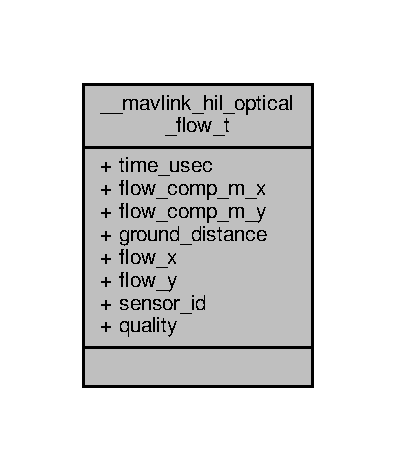
\includegraphics[width=190pt]{struct____mavlink__hil__optical__flow__t__coll__graph}
\end{center}
\end{figure}
\subsection*{Public Attributes}
\begin{DoxyCompactItemize}
\item 
\hypertarget{struct____mavlink__hil__optical__flow__t_abff1e3e4ebe3954eafe38491afdf10ee}{uint64\+\_\+t \hyperlink{struct____mavlink__hil__optical__flow__t_abff1e3e4ebe3954eafe38491afdf10ee}{time\+\_\+usec}}\label{struct____mavlink__hil__optical__flow__t_abff1e3e4ebe3954eafe38491afdf10ee}

\begin{DoxyCompactList}\small\item\em Timestamp (U\+N\+I\+X) \end{DoxyCompactList}\item 
\hypertarget{struct____mavlink__hil__optical__flow__t_acbc49d0debcfc63fddaf3194dcd964b2}{float \hyperlink{struct____mavlink__hil__optical__flow__t_acbc49d0debcfc63fddaf3194dcd964b2}{flow\+\_\+comp\+\_\+m\+\_\+x}}\label{struct____mavlink__hil__optical__flow__t_acbc49d0debcfc63fddaf3194dcd964b2}

\begin{DoxyCompactList}\small\item\em Flow in meters in x-\/sensor direction, angular-\/speed compensated. \end{DoxyCompactList}\item 
\hypertarget{struct____mavlink__hil__optical__flow__t_a474bf94c0c879bb240f4554e379073c5}{float \hyperlink{struct____mavlink__hil__optical__flow__t_a474bf94c0c879bb240f4554e379073c5}{flow\+\_\+comp\+\_\+m\+\_\+y}}\label{struct____mavlink__hil__optical__flow__t_a474bf94c0c879bb240f4554e379073c5}

\begin{DoxyCompactList}\small\item\em Flow in meters in y-\/sensor direction, angular-\/speed compensated. \end{DoxyCompactList}\item 
\hypertarget{struct____mavlink__hil__optical__flow__t_a0f4705c5970a0f4c6f75d93560fc0374}{float \hyperlink{struct____mavlink__hil__optical__flow__t_a0f4705c5970a0f4c6f75d93560fc0374}{ground\+\_\+distance}}\label{struct____mavlink__hil__optical__flow__t_a0f4705c5970a0f4c6f75d93560fc0374}

\begin{DoxyCompactList}\small\item\em Ground distance in meters. Positive value\+: distance known. Negative value\+: Unknown distance. \end{DoxyCompactList}\item 
\hypertarget{struct____mavlink__hil__optical__flow__t_a1592e86fb36d936682ecf4a9b4724a0a}{int16\+\_\+t \hyperlink{struct____mavlink__hil__optical__flow__t_a1592e86fb36d936682ecf4a9b4724a0a}{flow\+\_\+x}}\label{struct____mavlink__hil__optical__flow__t_a1592e86fb36d936682ecf4a9b4724a0a}

\begin{DoxyCompactList}\small\item\em Flow in pixels in x-\/sensor direction. \end{DoxyCompactList}\item 
\hypertarget{struct____mavlink__hil__optical__flow__t_a39c0b66d152bf2967aff1b505963dbbe}{int16\+\_\+t \hyperlink{struct____mavlink__hil__optical__flow__t_a39c0b66d152bf2967aff1b505963dbbe}{flow\+\_\+y}}\label{struct____mavlink__hil__optical__flow__t_a39c0b66d152bf2967aff1b505963dbbe}

\begin{DoxyCompactList}\small\item\em Flow in pixels in y-\/sensor direction. \end{DoxyCompactList}\item 
\hypertarget{struct____mavlink__hil__optical__flow__t_ac17ff8aa6f89d8bbed3915e21fb598a6}{uint8\+\_\+t \hyperlink{struct____mavlink__hil__optical__flow__t_ac17ff8aa6f89d8bbed3915e21fb598a6}{sensor\+\_\+id}}\label{struct____mavlink__hil__optical__flow__t_ac17ff8aa6f89d8bbed3915e21fb598a6}

\begin{DoxyCompactList}\small\item\em Sensor I\+D. \end{DoxyCompactList}\item 
\hypertarget{struct____mavlink__hil__optical__flow__t_a039f754e2192a783b41d3f6c2f62fe7d}{uint8\+\_\+t \hyperlink{struct____mavlink__hil__optical__flow__t_a039f754e2192a783b41d3f6c2f62fe7d}{quality}}\label{struct____mavlink__hil__optical__flow__t_a039f754e2192a783b41d3f6c2f62fe7d}

\begin{DoxyCompactList}\small\item\em Optical flow quality / confidence. 0\+: bad, 255\+: maximum quality. \end{DoxyCompactList}\end{DoxyCompactItemize}


The documentation for this struct was generated from the following file\+:\begin{DoxyCompactItemize}
\item 
/run/media/julien/\+Data/\+Documents/\+M\+A\+V\+R\+I\+C/\+M\+A\+V\+R\+I\+C\+\_\+\+Library/mavlink/include/maveric/mavlink\+\_\+msg\+\_\+hil\+\_\+optical\+\_\+flow.\+h\end{DoxyCompactItemize}

\hypertarget{struct____mavlink__hil__rc__inputs__raw__t}{\section{\+\_\+\+\_\+mavlink\+\_\+hil\+\_\+rc\+\_\+inputs\+\_\+raw\+\_\+t Struct Reference}
\label{struct____mavlink__hil__rc__inputs__raw__t}\index{\+\_\+\+\_\+mavlink\+\_\+hil\+\_\+rc\+\_\+inputs\+\_\+raw\+\_\+t@{\+\_\+\+\_\+mavlink\+\_\+hil\+\_\+rc\+\_\+inputs\+\_\+raw\+\_\+t}}
}


Collaboration diagram for \+\_\+\+\_\+mavlink\+\_\+hil\+\_\+rc\+\_\+inputs\+\_\+raw\+\_\+t\+:
\nopagebreak
\begin{figure}[H]
\begin{center}
\leavevmode
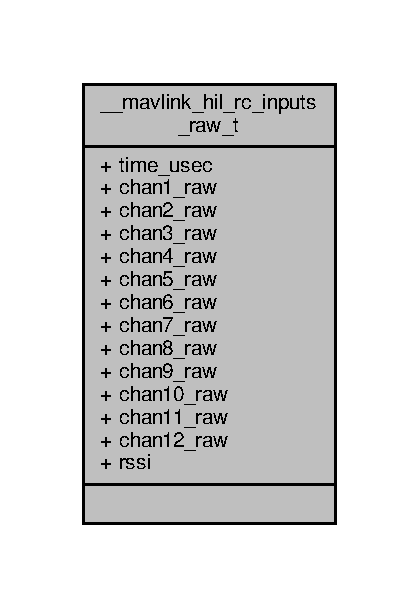
\includegraphics[width=201pt]{struct____mavlink__hil__rc__inputs__raw__t__coll__graph}
\end{center}
\end{figure}
\subsection*{Public Attributes}
\begin{DoxyCompactItemize}
\item 
\hypertarget{struct____mavlink__hil__rc__inputs__raw__t_a17665e54cab99a69ff2e6d3b8ae63928}{uint64\+\_\+t \hyperlink{struct____mavlink__hil__rc__inputs__raw__t_a17665e54cab99a69ff2e6d3b8ae63928}{time\+\_\+usec}}\label{struct____mavlink__hil__rc__inputs__raw__t_a17665e54cab99a69ff2e6d3b8ae63928}

\begin{DoxyCompactList}\small\item\em Timestamp (microseconds since U\+N\+I\+X epoch or microseconds since system boot) \end{DoxyCompactList}\item 
\hypertarget{struct____mavlink__hil__rc__inputs__raw__t_a1c71d0b0abbff7055c0753a8b8a116bc}{uint16\+\_\+t \hyperlink{struct____mavlink__hil__rc__inputs__raw__t_a1c71d0b0abbff7055c0753a8b8a116bc}{chan1\+\_\+raw}}\label{struct____mavlink__hil__rc__inputs__raw__t_a1c71d0b0abbff7055c0753a8b8a116bc}

\begin{DoxyCompactList}\small\item\em R\+C channel 1 value, in microseconds. \end{DoxyCompactList}\item 
\hypertarget{struct____mavlink__hil__rc__inputs__raw__t_a0210c7a3752c816e694c38e9fa85b8ed}{uint16\+\_\+t \hyperlink{struct____mavlink__hil__rc__inputs__raw__t_a0210c7a3752c816e694c38e9fa85b8ed}{chan2\+\_\+raw}}\label{struct____mavlink__hil__rc__inputs__raw__t_a0210c7a3752c816e694c38e9fa85b8ed}

\begin{DoxyCompactList}\small\item\em R\+C channel 2 value, in microseconds. \end{DoxyCompactList}\item 
\hypertarget{struct____mavlink__hil__rc__inputs__raw__t_a4f05c2ed52ec8aed527bc31331f74247}{uint16\+\_\+t \hyperlink{struct____mavlink__hil__rc__inputs__raw__t_a4f05c2ed52ec8aed527bc31331f74247}{chan3\+\_\+raw}}\label{struct____mavlink__hil__rc__inputs__raw__t_a4f05c2ed52ec8aed527bc31331f74247}

\begin{DoxyCompactList}\small\item\em R\+C channel 3 value, in microseconds. \end{DoxyCompactList}\item 
\hypertarget{struct____mavlink__hil__rc__inputs__raw__t_a762888a4e5d0273d9042bd1924c8b95b}{uint16\+\_\+t \hyperlink{struct____mavlink__hil__rc__inputs__raw__t_a762888a4e5d0273d9042bd1924c8b95b}{chan4\+\_\+raw}}\label{struct____mavlink__hil__rc__inputs__raw__t_a762888a4e5d0273d9042bd1924c8b95b}

\begin{DoxyCompactList}\small\item\em R\+C channel 4 value, in microseconds. \end{DoxyCompactList}\item 
\hypertarget{struct____mavlink__hil__rc__inputs__raw__t_aa351a492148d22983343be216e10e945}{uint16\+\_\+t \hyperlink{struct____mavlink__hil__rc__inputs__raw__t_aa351a492148d22983343be216e10e945}{chan5\+\_\+raw}}\label{struct____mavlink__hil__rc__inputs__raw__t_aa351a492148d22983343be216e10e945}

\begin{DoxyCompactList}\small\item\em R\+C channel 5 value, in microseconds. \end{DoxyCompactList}\item 
\hypertarget{struct____mavlink__hil__rc__inputs__raw__t_a861d32c4cee885839426c6c27e9985f7}{uint16\+\_\+t \hyperlink{struct____mavlink__hil__rc__inputs__raw__t_a861d32c4cee885839426c6c27e9985f7}{chan6\+\_\+raw}}\label{struct____mavlink__hil__rc__inputs__raw__t_a861d32c4cee885839426c6c27e9985f7}

\begin{DoxyCompactList}\small\item\em R\+C channel 6 value, in microseconds. \end{DoxyCompactList}\item 
\hypertarget{struct____mavlink__hil__rc__inputs__raw__t_a58471d376608366dc4e762c1cc07f0da}{uint16\+\_\+t \hyperlink{struct____mavlink__hil__rc__inputs__raw__t_a58471d376608366dc4e762c1cc07f0da}{chan7\+\_\+raw}}\label{struct____mavlink__hil__rc__inputs__raw__t_a58471d376608366dc4e762c1cc07f0da}

\begin{DoxyCompactList}\small\item\em R\+C channel 7 value, in microseconds. \end{DoxyCompactList}\item 
\hypertarget{struct____mavlink__hil__rc__inputs__raw__t_a5e2a946b0960b971317637874d4f2678}{uint16\+\_\+t \hyperlink{struct____mavlink__hil__rc__inputs__raw__t_a5e2a946b0960b971317637874d4f2678}{chan8\+\_\+raw}}\label{struct____mavlink__hil__rc__inputs__raw__t_a5e2a946b0960b971317637874d4f2678}

\begin{DoxyCompactList}\small\item\em R\+C channel 8 value, in microseconds. \end{DoxyCompactList}\item 
\hypertarget{struct____mavlink__hil__rc__inputs__raw__t_aebe7c293f27d5b25c78caa8f762c57e2}{uint16\+\_\+t \hyperlink{struct____mavlink__hil__rc__inputs__raw__t_aebe7c293f27d5b25c78caa8f762c57e2}{chan9\+\_\+raw}}\label{struct____mavlink__hil__rc__inputs__raw__t_aebe7c293f27d5b25c78caa8f762c57e2}

\begin{DoxyCompactList}\small\item\em R\+C channel 9 value, in microseconds. \end{DoxyCompactList}\item 
\hypertarget{struct____mavlink__hil__rc__inputs__raw__t_ac49fe649301c639a71ae5a5778934a3c}{uint16\+\_\+t \hyperlink{struct____mavlink__hil__rc__inputs__raw__t_ac49fe649301c639a71ae5a5778934a3c}{chan10\+\_\+raw}}\label{struct____mavlink__hil__rc__inputs__raw__t_ac49fe649301c639a71ae5a5778934a3c}

\begin{DoxyCompactList}\small\item\em R\+C channel 10 value, in microseconds. \end{DoxyCompactList}\item 
\hypertarget{struct____mavlink__hil__rc__inputs__raw__t_a09b92c1ec569948809c152e74bd61655}{uint16\+\_\+t \hyperlink{struct____mavlink__hil__rc__inputs__raw__t_a09b92c1ec569948809c152e74bd61655}{chan11\+\_\+raw}}\label{struct____mavlink__hil__rc__inputs__raw__t_a09b92c1ec569948809c152e74bd61655}

\begin{DoxyCompactList}\small\item\em R\+C channel 11 value, in microseconds. \end{DoxyCompactList}\item 
\hypertarget{struct____mavlink__hil__rc__inputs__raw__t_a5967e01d1c858a6136505185d183a99e}{uint16\+\_\+t \hyperlink{struct____mavlink__hil__rc__inputs__raw__t_a5967e01d1c858a6136505185d183a99e}{chan12\+\_\+raw}}\label{struct____mavlink__hil__rc__inputs__raw__t_a5967e01d1c858a6136505185d183a99e}

\begin{DoxyCompactList}\small\item\em R\+C channel 12 value, in microseconds. \end{DoxyCompactList}\item 
\hypertarget{struct____mavlink__hil__rc__inputs__raw__t_aa126d8b574a26544c57605c5aa1f8684}{uint8\+\_\+t \hyperlink{struct____mavlink__hil__rc__inputs__raw__t_aa126d8b574a26544c57605c5aa1f8684}{rssi}}\label{struct____mavlink__hil__rc__inputs__raw__t_aa126d8b574a26544c57605c5aa1f8684}

\begin{DoxyCompactList}\small\item\em Receive signal strength indicator, 0\+: 0\%, 255\+: 100\%. \end{DoxyCompactList}\end{DoxyCompactItemize}


The documentation for this struct was generated from the following file\+:\begin{DoxyCompactItemize}
\item 
/run/media/julien/\+Data/\+Documents/\+M\+A\+V\+R\+I\+C/\+M\+A\+V\+R\+I\+C\+\_\+\+Library/mavlink/include/common/mavlink\+\_\+msg\+\_\+hil\+\_\+rc\+\_\+inputs\+\_\+raw.\+h\end{DoxyCompactItemize}

\hypertarget{struct____mavlink__hil__sensor__t}{\section{\+\_\+\+\_\+mavlink\+\_\+hil\+\_\+sensor\+\_\+t Struct Reference}
\label{struct____mavlink__hil__sensor__t}\index{\+\_\+\+\_\+mavlink\+\_\+hil\+\_\+sensor\+\_\+t@{\+\_\+\+\_\+mavlink\+\_\+hil\+\_\+sensor\+\_\+t}}
}


Collaboration diagram for \+\_\+\+\_\+mavlink\+\_\+hil\+\_\+sensor\+\_\+t\+:
\nopagebreak
\begin{figure}[H]
\begin{center}
\leavevmode
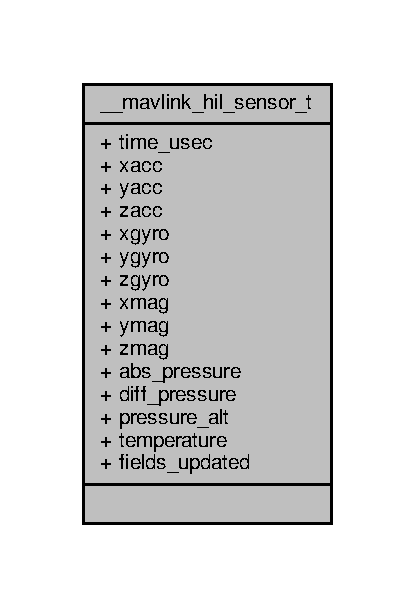
\includegraphics[width=199pt]{struct____mavlink__hil__sensor__t__coll__graph}
\end{center}
\end{figure}
\subsection*{Public Attributes}
\begin{DoxyCompactItemize}
\item 
\hypertarget{struct____mavlink__hil__sensor__t_a45de41520af13fd33f21c82c72a98b75}{uint64\+\_\+t \hyperlink{struct____mavlink__hil__sensor__t_a45de41520af13fd33f21c82c72a98b75}{time\+\_\+usec}}\label{struct____mavlink__hil__sensor__t_a45de41520af13fd33f21c82c72a98b75}

\begin{DoxyCompactList}\small\item\em Timestamp (microseconds, synced to U\+N\+I\+X time or since system boot) \end{DoxyCompactList}\item 
\hypertarget{struct____mavlink__hil__sensor__t_a20c3e6c7f8dd61b698cb617ec76c4b9d}{float \hyperlink{struct____mavlink__hil__sensor__t_a20c3e6c7f8dd61b698cb617ec76c4b9d}{xacc}}\label{struct____mavlink__hil__sensor__t_a20c3e6c7f8dd61b698cb617ec76c4b9d}

\begin{DoxyCompactList}\small\item\em X acceleration (m/s$^\wedge$2) \end{DoxyCompactList}\item 
\hypertarget{struct____mavlink__hil__sensor__t_a3649b04bdbc3d90b3c8da37b6ab02d6c}{float \hyperlink{struct____mavlink__hil__sensor__t_a3649b04bdbc3d90b3c8da37b6ab02d6c}{yacc}}\label{struct____mavlink__hil__sensor__t_a3649b04bdbc3d90b3c8da37b6ab02d6c}

\begin{DoxyCompactList}\small\item\em Y acceleration (m/s$^\wedge$2) \end{DoxyCompactList}\item 
\hypertarget{struct____mavlink__hil__sensor__t_acbecb9b5205c1b4fa0c43c2c45f78b4d}{float \hyperlink{struct____mavlink__hil__sensor__t_acbecb9b5205c1b4fa0c43c2c45f78b4d}{zacc}}\label{struct____mavlink__hil__sensor__t_acbecb9b5205c1b4fa0c43c2c45f78b4d}

\begin{DoxyCompactList}\small\item\em Z acceleration (m/s$^\wedge$2) \end{DoxyCompactList}\item 
\hypertarget{struct____mavlink__hil__sensor__t_a3b4035c288cba98923051942dfd85dc0}{float \hyperlink{struct____mavlink__hil__sensor__t_a3b4035c288cba98923051942dfd85dc0}{xgyro}}\label{struct____mavlink__hil__sensor__t_a3b4035c288cba98923051942dfd85dc0}

\begin{DoxyCompactList}\small\item\em Angular speed around X axis in body frame (rad / sec) \end{DoxyCompactList}\item 
\hypertarget{struct____mavlink__hil__sensor__t_abdeea02a356a5802b5580fdd945bcbe6}{float \hyperlink{struct____mavlink__hil__sensor__t_abdeea02a356a5802b5580fdd945bcbe6}{ygyro}}\label{struct____mavlink__hil__sensor__t_abdeea02a356a5802b5580fdd945bcbe6}

\begin{DoxyCompactList}\small\item\em Angular speed around Y axis in body frame (rad / sec) \end{DoxyCompactList}\item 
\hypertarget{struct____mavlink__hil__sensor__t_ab7c2f35160da57fecb77a7e6b7d48dc9}{float \hyperlink{struct____mavlink__hil__sensor__t_ab7c2f35160da57fecb77a7e6b7d48dc9}{zgyro}}\label{struct____mavlink__hil__sensor__t_ab7c2f35160da57fecb77a7e6b7d48dc9}

\begin{DoxyCompactList}\small\item\em Angular speed around Z axis in body frame (rad / sec) \end{DoxyCompactList}\item 
\hypertarget{struct____mavlink__hil__sensor__t_a246f9f9b48771987750d94e15a0465f3}{float \hyperlink{struct____mavlink__hil__sensor__t_a246f9f9b48771987750d94e15a0465f3}{xmag}}\label{struct____mavlink__hil__sensor__t_a246f9f9b48771987750d94e15a0465f3}

\begin{DoxyCompactList}\small\item\em X Magnetic field (Gauss) \end{DoxyCompactList}\item 
\hypertarget{struct____mavlink__hil__sensor__t_a0693da306eb0d30f2b5502e51540d05b}{float \hyperlink{struct____mavlink__hil__sensor__t_a0693da306eb0d30f2b5502e51540d05b}{ymag}}\label{struct____mavlink__hil__sensor__t_a0693da306eb0d30f2b5502e51540d05b}

\begin{DoxyCompactList}\small\item\em Y Magnetic field (Gauss) \end{DoxyCompactList}\item 
\hypertarget{struct____mavlink__hil__sensor__t_a6db8180441080e7dcccfda7da09b1e2d}{float \hyperlink{struct____mavlink__hil__sensor__t_a6db8180441080e7dcccfda7da09b1e2d}{zmag}}\label{struct____mavlink__hil__sensor__t_a6db8180441080e7dcccfda7da09b1e2d}

\begin{DoxyCompactList}\small\item\em Z Magnetic field (Gauss) \end{DoxyCompactList}\item 
\hypertarget{struct____mavlink__hil__sensor__t_a7d05535dddd4be7c92b616ea644cb6cd}{float \hyperlink{struct____mavlink__hil__sensor__t_a7d05535dddd4be7c92b616ea644cb6cd}{abs\+\_\+pressure}}\label{struct____mavlink__hil__sensor__t_a7d05535dddd4be7c92b616ea644cb6cd}

\begin{DoxyCompactList}\small\item\em Absolute pressure in millibar. \end{DoxyCompactList}\item 
\hypertarget{struct____mavlink__hil__sensor__t_a614e2fe0a712bc9619669950f09dd21d}{float \hyperlink{struct____mavlink__hil__sensor__t_a614e2fe0a712bc9619669950f09dd21d}{diff\+\_\+pressure}}\label{struct____mavlink__hil__sensor__t_a614e2fe0a712bc9619669950f09dd21d}

\begin{DoxyCompactList}\small\item\em Differential pressure (airspeed) in millibar. \end{DoxyCompactList}\item 
\hypertarget{struct____mavlink__hil__sensor__t_aa7347c28c478d103f181d57aee8026de}{float \hyperlink{struct____mavlink__hil__sensor__t_aa7347c28c478d103f181d57aee8026de}{pressure\+\_\+alt}}\label{struct____mavlink__hil__sensor__t_aa7347c28c478d103f181d57aee8026de}

\begin{DoxyCompactList}\small\item\em Altitude calculated from pressure. \end{DoxyCompactList}\item 
\hypertarget{struct____mavlink__hil__sensor__t_a775825e9a485480f835e1b01c9ef878a}{float \hyperlink{struct____mavlink__hil__sensor__t_a775825e9a485480f835e1b01c9ef878a}{temperature}}\label{struct____mavlink__hil__sensor__t_a775825e9a485480f835e1b01c9ef878a}

\begin{DoxyCompactList}\small\item\em Temperature in degrees celsius. \end{DoxyCompactList}\item 
\hypertarget{struct____mavlink__hil__sensor__t_a47ccb8d87933c760160e5f6f513f0e90}{uint32\+\_\+t \hyperlink{struct____mavlink__hil__sensor__t_a47ccb8d87933c760160e5f6f513f0e90}{fields\+\_\+updated}}\label{struct____mavlink__hil__sensor__t_a47ccb8d87933c760160e5f6f513f0e90}

\begin{DoxyCompactList}\small\item\em Bitmask for fields that have updated since last message, bit 0 = xacc, bit 12\+: temperature. \end{DoxyCompactList}\end{DoxyCompactItemize}


The documentation for this struct was generated from the following file\+:\begin{DoxyCompactItemize}
\item 
/run/media/julien/\+Data/\+Documents/\+M\+A\+V\+R\+I\+C/\+M\+A\+V\+R\+I\+C\+\_\+\+Library/mavlink/include/maveric/mavlink\+\_\+msg\+\_\+hil\+\_\+sensor.\+h\end{DoxyCompactItemize}

\hypertarget{struct____mavlink__hil__state__quaternion__t}{\section{\+\_\+\+\_\+mavlink\+\_\+hil\+\_\+state\+\_\+quaternion\+\_\+t Struct Reference}
\label{struct____mavlink__hil__state__quaternion__t}\index{\+\_\+\+\_\+mavlink\+\_\+hil\+\_\+state\+\_\+quaternion\+\_\+t@{\+\_\+\+\_\+mavlink\+\_\+hil\+\_\+state\+\_\+quaternion\+\_\+t}}
}


Collaboration diagram for \+\_\+\+\_\+mavlink\+\_\+hil\+\_\+state\+\_\+quaternion\+\_\+t\+:
\nopagebreak
\begin{figure}[H]
\begin{center}
\leavevmode
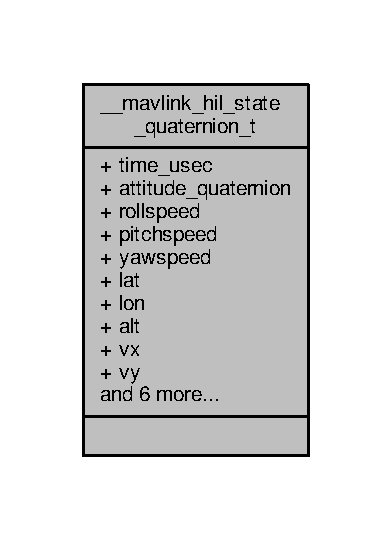
\includegraphics[width=188pt]{struct____mavlink__hil__state__quaternion__t__coll__graph}
\end{center}
\end{figure}
\subsection*{Public Attributes}
\begin{DoxyCompactItemize}
\item 
\hypertarget{struct____mavlink__hil__state__quaternion__t_a15c7dccf96d2c5087b171d388dd775d8}{uint64\+\_\+t \hyperlink{struct____mavlink__hil__state__quaternion__t_a15c7dccf96d2c5087b171d388dd775d8}{time\+\_\+usec}}\label{struct____mavlink__hil__state__quaternion__t_a15c7dccf96d2c5087b171d388dd775d8}

\begin{DoxyCompactList}\small\item\em Timestamp (microseconds since U\+N\+I\+X epoch or microseconds since system boot) \end{DoxyCompactList}\item 
\hypertarget{struct____mavlink__hil__state__quaternion__t_a52878cf5515b47e1db662b326c169e64}{float \hyperlink{struct____mavlink__hil__state__quaternion__t_a52878cf5515b47e1db662b326c169e64}{attitude\+\_\+quaternion} \mbox{[}4\mbox{]}}\label{struct____mavlink__hil__state__quaternion__t_a52878cf5515b47e1db662b326c169e64}

\begin{DoxyCompactList}\small\item\em Vehicle attitude expressed as normalized quaternion. \end{DoxyCompactList}\item 
\hypertarget{struct____mavlink__hil__state__quaternion__t_a83042286abfe3545cabe2d4e5a087f12}{float \hyperlink{struct____mavlink__hil__state__quaternion__t_a83042286abfe3545cabe2d4e5a087f12}{rollspeed}}\label{struct____mavlink__hil__state__quaternion__t_a83042286abfe3545cabe2d4e5a087f12}

\begin{DoxyCompactList}\small\item\em Body frame roll / phi angular speed (rad/s) \end{DoxyCompactList}\item 
\hypertarget{struct____mavlink__hil__state__quaternion__t_a68900f55507fd4fb1dfcf1687fb292ed}{float \hyperlink{struct____mavlink__hil__state__quaternion__t_a68900f55507fd4fb1dfcf1687fb292ed}{pitchspeed}}\label{struct____mavlink__hil__state__quaternion__t_a68900f55507fd4fb1dfcf1687fb292ed}

\begin{DoxyCompactList}\small\item\em Body frame pitch / theta angular speed (rad/s) \end{DoxyCompactList}\item 
\hypertarget{struct____mavlink__hil__state__quaternion__t_ab3474522e90658e09da1a3bfaa235fab}{float \hyperlink{struct____mavlink__hil__state__quaternion__t_ab3474522e90658e09da1a3bfaa235fab}{yawspeed}}\label{struct____mavlink__hil__state__quaternion__t_ab3474522e90658e09da1a3bfaa235fab}

\begin{DoxyCompactList}\small\item\em Body frame yaw / psi angular speed (rad/s) \end{DoxyCompactList}\item 
\hypertarget{struct____mavlink__hil__state__quaternion__t_a2e54416e81eb004268570f4250242356}{int32\+\_\+t \hyperlink{struct____mavlink__hil__state__quaternion__t_a2e54416e81eb004268570f4250242356}{lat}}\label{struct____mavlink__hil__state__quaternion__t_a2e54416e81eb004268570f4250242356}

\begin{DoxyCompactList}\small\item\em Latitude, expressed as $\ast$ 1\+E7. \end{DoxyCompactList}\item 
\hypertarget{struct____mavlink__hil__state__quaternion__t_a345f022044f481073ea518e0ac65218a}{int32\+\_\+t \hyperlink{struct____mavlink__hil__state__quaternion__t_a345f022044f481073ea518e0ac65218a}{lon}}\label{struct____mavlink__hil__state__quaternion__t_a345f022044f481073ea518e0ac65218a}

\begin{DoxyCompactList}\small\item\em Longitude, expressed as $\ast$ 1\+E7. \end{DoxyCompactList}\item 
\hypertarget{struct____mavlink__hil__state__quaternion__t_abde8333e57ef71852b1de1529f3f3146}{int32\+\_\+t \hyperlink{struct____mavlink__hil__state__quaternion__t_abde8333e57ef71852b1de1529f3f3146}{alt}}\label{struct____mavlink__hil__state__quaternion__t_abde8333e57ef71852b1de1529f3f3146}

\begin{DoxyCompactList}\small\item\em Altitude in meters, expressed as $\ast$ 1000 (millimeters) \end{DoxyCompactList}\item 
\hypertarget{struct____mavlink__hil__state__quaternion__t_a0c33d3ef8decf225d84201d19b5da35f}{int16\+\_\+t \hyperlink{struct____mavlink__hil__state__quaternion__t_a0c33d3ef8decf225d84201d19b5da35f}{vx}}\label{struct____mavlink__hil__state__quaternion__t_a0c33d3ef8decf225d84201d19b5da35f}

\begin{DoxyCompactList}\small\item\em Ground X Speed (Latitude), expressed as m/s $\ast$ 100. \end{DoxyCompactList}\item 
\hypertarget{struct____mavlink__hil__state__quaternion__t_ae13c1fd1447d434847c4791181e270c1}{int16\+\_\+t \hyperlink{struct____mavlink__hil__state__quaternion__t_ae13c1fd1447d434847c4791181e270c1}{vy}}\label{struct____mavlink__hil__state__quaternion__t_ae13c1fd1447d434847c4791181e270c1}

\begin{DoxyCompactList}\small\item\em Ground Y Speed (Longitude), expressed as m/s $\ast$ 100. \end{DoxyCompactList}\item 
\hypertarget{struct____mavlink__hil__state__quaternion__t_a40093764fa265d7443ce5d6215bc6cfa}{int16\+\_\+t \hyperlink{struct____mavlink__hil__state__quaternion__t_a40093764fa265d7443ce5d6215bc6cfa}{vz}}\label{struct____mavlink__hil__state__quaternion__t_a40093764fa265d7443ce5d6215bc6cfa}

\begin{DoxyCompactList}\small\item\em Ground Z Speed (Altitude), expressed as m/s $\ast$ 100. \end{DoxyCompactList}\item 
\hypertarget{struct____mavlink__hil__state__quaternion__t_a78c835fba2a49d66fd73d745d347fac5}{uint16\+\_\+t \hyperlink{struct____mavlink__hil__state__quaternion__t_a78c835fba2a49d66fd73d745d347fac5}{ind\+\_\+airspeed}}\label{struct____mavlink__hil__state__quaternion__t_a78c835fba2a49d66fd73d745d347fac5}

\begin{DoxyCompactList}\small\item\em Indicated airspeed, expressed as m/s $\ast$ 100. \end{DoxyCompactList}\item 
\hypertarget{struct____mavlink__hil__state__quaternion__t_ac644e31d08eeed05f5f3b7eacdd18f4b}{uint16\+\_\+t \hyperlink{struct____mavlink__hil__state__quaternion__t_ac644e31d08eeed05f5f3b7eacdd18f4b}{true\+\_\+airspeed}}\label{struct____mavlink__hil__state__quaternion__t_ac644e31d08eeed05f5f3b7eacdd18f4b}

\begin{DoxyCompactList}\small\item\em True airspeed, expressed as m/s $\ast$ 100. \end{DoxyCompactList}\item 
\hypertarget{struct____mavlink__hil__state__quaternion__t_a72af144dbb58ba6cd5a474206a88420f}{int16\+\_\+t \hyperlink{struct____mavlink__hil__state__quaternion__t_a72af144dbb58ba6cd5a474206a88420f}{xacc}}\label{struct____mavlink__hil__state__quaternion__t_a72af144dbb58ba6cd5a474206a88420f}

\begin{DoxyCompactList}\small\item\em X acceleration (mg) \end{DoxyCompactList}\item 
\hypertarget{struct____mavlink__hil__state__quaternion__t_a949a82c6d368468354dd201cda5458fa}{int16\+\_\+t \hyperlink{struct____mavlink__hil__state__quaternion__t_a949a82c6d368468354dd201cda5458fa}{yacc}}\label{struct____mavlink__hil__state__quaternion__t_a949a82c6d368468354dd201cda5458fa}

\begin{DoxyCompactList}\small\item\em Y acceleration (mg) \end{DoxyCompactList}\item 
\hypertarget{struct____mavlink__hil__state__quaternion__t_a8e4533aa8c582bf609a813b65835fe52}{int16\+\_\+t \hyperlink{struct____mavlink__hil__state__quaternion__t_a8e4533aa8c582bf609a813b65835fe52}{zacc}}\label{struct____mavlink__hil__state__quaternion__t_a8e4533aa8c582bf609a813b65835fe52}

\begin{DoxyCompactList}\small\item\em Z acceleration (mg) \end{DoxyCompactList}\end{DoxyCompactItemize}


The documentation for this struct was generated from the following file\+:\begin{DoxyCompactItemize}
\item 
/run/media/julien/\+Data/\+Documents/\+M\+A\+V\+R\+I\+C/\+M\+A\+V\+R\+I\+C\+\_\+\+Library/mavlink/include/maveric/mavlink\+\_\+msg\+\_\+hil\+\_\+state\+\_\+quaternion.\+h\end{DoxyCompactItemize}

\hypertarget{struct____mavlink__hil__state__t}{\section{\+\_\+\+\_\+mavlink\+\_\+hil\+\_\+state\+\_\+t Struct Reference}
\label{struct____mavlink__hil__state__t}\index{\+\_\+\+\_\+mavlink\+\_\+hil\+\_\+state\+\_\+t@{\+\_\+\+\_\+mavlink\+\_\+hil\+\_\+state\+\_\+t}}
}


Collaboration diagram for \+\_\+\+\_\+mavlink\+\_\+hil\+\_\+state\+\_\+t\+:
\nopagebreak
\begin{figure}[H]
\begin{center}
\leavevmode
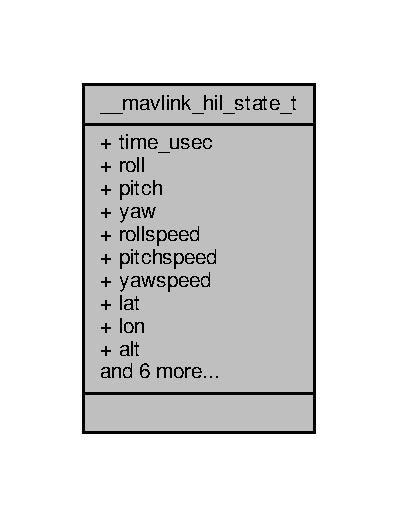
\includegraphics[width=191pt]{struct____mavlink__hil__state__t__coll__graph}
\end{center}
\end{figure}
\subsection*{Public Attributes}
\begin{DoxyCompactItemize}
\item 
\hypertarget{struct____mavlink__hil__state__t_a19f9efdaaddd6d9699f8225bf5a4d4ef}{uint64\+\_\+t \hyperlink{struct____mavlink__hil__state__t_a19f9efdaaddd6d9699f8225bf5a4d4ef}{time\+\_\+usec}}\label{struct____mavlink__hil__state__t_a19f9efdaaddd6d9699f8225bf5a4d4ef}

\begin{DoxyCompactList}\small\item\em Timestamp (microseconds since U\+N\+I\+X epoch or microseconds since system boot) \end{DoxyCompactList}\item 
\hypertarget{struct____mavlink__hil__state__t_a33202a922fda8d956b7ce78814d82558}{float \hyperlink{struct____mavlink__hil__state__t_a33202a922fda8d956b7ce78814d82558}{roll}}\label{struct____mavlink__hil__state__t_a33202a922fda8d956b7ce78814d82558}

\begin{DoxyCompactList}\small\item\em Roll angle (rad) \end{DoxyCompactList}\item 
\hypertarget{struct____mavlink__hil__state__t_a734b8ba645687e5673c599c4a9a950f1}{float \hyperlink{struct____mavlink__hil__state__t_a734b8ba645687e5673c599c4a9a950f1}{pitch}}\label{struct____mavlink__hil__state__t_a734b8ba645687e5673c599c4a9a950f1}

\begin{DoxyCompactList}\small\item\em Pitch angle (rad) \end{DoxyCompactList}\item 
\hypertarget{struct____mavlink__hil__state__t_aa7a7dfae39434c0c51492cb2d5614863}{float \hyperlink{struct____mavlink__hil__state__t_aa7a7dfae39434c0c51492cb2d5614863}{yaw}}\label{struct____mavlink__hil__state__t_aa7a7dfae39434c0c51492cb2d5614863}

\begin{DoxyCompactList}\small\item\em Yaw angle (rad) \end{DoxyCompactList}\item 
float \hyperlink{struct____mavlink__hil__state__t_a308aa515448a4d8d25131ce7c0f3254d}{rollspeed}
\begin{DoxyCompactList}\small\item\em Roll angular speed (rad/s) \end{DoxyCompactList}\item 
float \hyperlink{struct____mavlink__hil__state__t_ad7d8b42ee6698e6f892c20146f954d5a}{pitchspeed}
\begin{DoxyCompactList}\small\item\em Pitch angular speed (rad/s) \end{DoxyCompactList}\item 
float \hyperlink{struct____mavlink__hil__state__t_a50f16fd863e535867c95fabcfef2e498}{yawspeed}
\begin{DoxyCompactList}\small\item\em Yaw angular speed (rad/s) \end{DoxyCompactList}\item 
\hypertarget{struct____mavlink__hil__state__t_afb2b29710c1a8b69503e35a72473c6d3}{int32\+\_\+t \hyperlink{struct____mavlink__hil__state__t_afb2b29710c1a8b69503e35a72473c6d3}{lat}}\label{struct____mavlink__hil__state__t_afb2b29710c1a8b69503e35a72473c6d3}

\begin{DoxyCompactList}\small\item\em Latitude, expressed as $\ast$ 1\+E7. \end{DoxyCompactList}\item 
\hypertarget{struct____mavlink__hil__state__t_aeac8427298a17d090889edf71a21c6ac}{int32\+\_\+t \hyperlink{struct____mavlink__hil__state__t_aeac8427298a17d090889edf71a21c6ac}{lon}}\label{struct____mavlink__hil__state__t_aeac8427298a17d090889edf71a21c6ac}

\begin{DoxyCompactList}\small\item\em Longitude, expressed as $\ast$ 1\+E7. \end{DoxyCompactList}\item 
\hypertarget{struct____mavlink__hil__state__t_a8f4ac2f2f4948df71b4abbb50d7c2f2f}{int32\+\_\+t \hyperlink{struct____mavlink__hil__state__t_a8f4ac2f2f4948df71b4abbb50d7c2f2f}{alt}}\label{struct____mavlink__hil__state__t_a8f4ac2f2f4948df71b4abbb50d7c2f2f}

\begin{DoxyCompactList}\small\item\em Altitude in meters, expressed as $\ast$ 1000 (millimeters) \end{DoxyCompactList}\item 
\hypertarget{struct____mavlink__hil__state__t_a8ea365258210e69427e6c02f82aa710c}{int16\+\_\+t \hyperlink{struct____mavlink__hil__state__t_a8ea365258210e69427e6c02f82aa710c}{vx}}\label{struct____mavlink__hil__state__t_a8ea365258210e69427e6c02f82aa710c}

\begin{DoxyCompactList}\small\item\em Ground X Speed (Latitude), expressed as m/s $\ast$ 100. \end{DoxyCompactList}\item 
\hypertarget{struct____mavlink__hil__state__t_a8d3234cf343035ab3f240f23fac95072}{int16\+\_\+t \hyperlink{struct____mavlink__hil__state__t_a8d3234cf343035ab3f240f23fac95072}{vy}}\label{struct____mavlink__hil__state__t_a8d3234cf343035ab3f240f23fac95072}

\begin{DoxyCompactList}\small\item\em Ground Y Speed (Longitude), expressed as m/s $\ast$ 100. \end{DoxyCompactList}\item 
\hypertarget{struct____mavlink__hil__state__t_add6c834de56047ff2316d059b741cce0}{int16\+\_\+t \hyperlink{struct____mavlink__hil__state__t_add6c834de56047ff2316d059b741cce0}{vz}}\label{struct____mavlink__hil__state__t_add6c834de56047ff2316d059b741cce0}

\begin{DoxyCompactList}\small\item\em Ground Z Speed (Altitude), expressed as m/s $\ast$ 100. \end{DoxyCompactList}\item 
\hypertarget{struct____mavlink__hil__state__t_a8497c1e566b9acb1d4298090c480a212}{int16\+\_\+t \hyperlink{struct____mavlink__hil__state__t_a8497c1e566b9acb1d4298090c480a212}{xacc}}\label{struct____mavlink__hil__state__t_a8497c1e566b9acb1d4298090c480a212}

\begin{DoxyCompactList}\small\item\em X acceleration (mg) \end{DoxyCompactList}\item 
\hypertarget{struct____mavlink__hil__state__t_a670623660d6d3d15121b2698082e8f55}{int16\+\_\+t \hyperlink{struct____mavlink__hil__state__t_a670623660d6d3d15121b2698082e8f55}{yacc}}\label{struct____mavlink__hil__state__t_a670623660d6d3d15121b2698082e8f55}

\begin{DoxyCompactList}\small\item\em Y acceleration (mg) \end{DoxyCompactList}\item 
\hypertarget{struct____mavlink__hil__state__t_a79b626e6b13844d733a6a6c02e506b90}{int16\+\_\+t \hyperlink{struct____mavlink__hil__state__t_a79b626e6b13844d733a6a6c02e506b90}{zacc}}\label{struct____mavlink__hil__state__t_a79b626e6b13844d733a6a6c02e506b90}

\begin{DoxyCompactList}\small\item\em Z acceleration (mg) \end{DoxyCompactList}\end{DoxyCompactItemize}


\subsection{Member Data Documentation}
\hypertarget{struct____mavlink__hil__state__t_ad7d8b42ee6698e6f892c20146f954d5a}{\index{\+\_\+\+\_\+mavlink\+\_\+hil\+\_\+state\+\_\+t@{\+\_\+\+\_\+mavlink\+\_\+hil\+\_\+state\+\_\+t}!pitchspeed@{pitchspeed}}
\index{pitchspeed@{pitchspeed}!\+\_\+\+\_\+mavlink\+\_\+hil\+\_\+state\+\_\+t@{\+\_\+\+\_\+mavlink\+\_\+hil\+\_\+state\+\_\+t}}
\subsubsection[{pitchspeed}]{\setlength{\rightskip}{0pt plus 5cm}float \+\_\+\+\_\+mavlink\+\_\+hil\+\_\+state\+\_\+t\+::pitchspeed}}\label{struct____mavlink__hil__state__t_ad7d8b42ee6698e6f892c20146f954d5a}


Pitch angular speed (rad/s) 

Body frame pitch / theta angular speed (rad/s) \hypertarget{struct____mavlink__hil__state__t_a308aa515448a4d8d25131ce7c0f3254d}{\index{\+\_\+\+\_\+mavlink\+\_\+hil\+\_\+state\+\_\+t@{\+\_\+\+\_\+mavlink\+\_\+hil\+\_\+state\+\_\+t}!rollspeed@{rollspeed}}
\index{rollspeed@{rollspeed}!\+\_\+\+\_\+mavlink\+\_\+hil\+\_\+state\+\_\+t@{\+\_\+\+\_\+mavlink\+\_\+hil\+\_\+state\+\_\+t}}
\subsubsection[{rollspeed}]{\setlength{\rightskip}{0pt plus 5cm}float \+\_\+\+\_\+mavlink\+\_\+hil\+\_\+state\+\_\+t\+::rollspeed}}\label{struct____mavlink__hil__state__t_a308aa515448a4d8d25131ce7c0f3254d}


Roll angular speed (rad/s) 

Body frame roll / phi angular speed (rad/s) \hypertarget{struct____mavlink__hil__state__t_a50f16fd863e535867c95fabcfef2e498}{\index{\+\_\+\+\_\+mavlink\+\_\+hil\+\_\+state\+\_\+t@{\+\_\+\+\_\+mavlink\+\_\+hil\+\_\+state\+\_\+t}!yawspeed@{yawspeed}}
\index{yawspeed@{yawspeed}!\+\_\+\+\_\+mavlink\+\_\+hil\+\_\+state\+\_\+t@{\+\_\+\+\_\+mavlink\+\_\+hil\+\_\+state\+\_\+t}}
\subsubsection[{yawspeed}]{\setlength{\rightskip}{0pt plus 5cm}float \+\_\+\+\_\+mavlink\+\_\+hil\+\_\+state\+\_\+t\+::yawspeed}}\label{struct____mavlink__hil__state__t_a50f16fd863e535867c95fabcfef2e498}


Yaw angular speed (rad/s) 

Body frame yaw / psi angular speed (rad/s) 

The documentation for this struct was generated from the following file\+:\begin{DoxyCompactItemize}
\item 
/run/media/julien/\+Data/\+Documents/\+M\+A\+V\+R\+I\+C/\+M\+A\+V\+R\+I\+C\+\_\+\+Library/mavlink/include/common/mavlink\+\_\+msg\+\_\+hil\+\_\+state.\+h\end{DoxyCompactItemize}

\hypertarget{struct____mavlink__local__position__ned__system__global__offset__t}{\section{\+\_\+\+\_\+mavlink\+\_\+local\+\_\+position\+\_\+ned\+\_\+system\+\_\+global\+\_\+offset\+\_\+t Struct Reference}
\label{struct____mavlink__local__position__ned__system__global__offset__t}\index{\+\_\+\+\_\+mavlink\+\_\+local\+\_\+position\+\_\+ned\+\_\+system\+\_\+global\+\_\+offset\+\_\+t@{\+\_\+\+\_\+mavlink\+\_\+local\+\_\+position\+\_\+ned\+\_\+system\+\_\+global\+\_\+offset\+\_\+t}}
}


Collaboration diagram for \+\_\+\+\_\+mavlink\+\_\+local\+\_\+position\+\_\+ned\+\_\+system\+\_\+global\+\_\+offset\+\_\+t\+:
\nopagebreak
\begin{figure}[H]
\begin{center}
\leavevmode
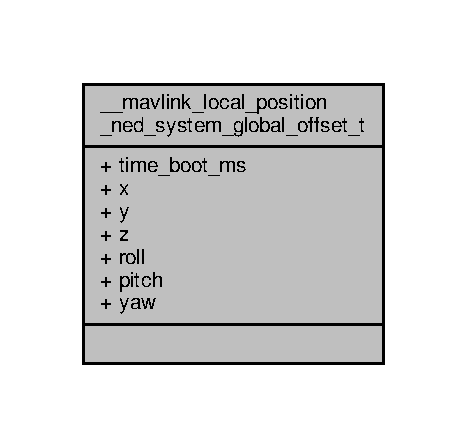
\includegraphics[width=224pt]{struct____mavlink__local__position__ned__system__global__offset__t__coll__graph}
\end{center}
\end{figure}
\subsection*{Public Attributes}
\begin{DoxyCompactItemize}
\item 
\hypertarget{struct____mavlink__local__position__ned__system__global__offset__t_a7da6dfcadb9fe7e050d067ab139600c4}{uint32\+\_\+t \hyperlink{struct____mavlink__local__position__ned__system__global__offset__t_a7da6dfcadb9fe7e050d067ab139600c4}{time\+\_\+boot\+\_\+ms}}\label{struct____mavlink__local__position__ned__system__global__offset__t_a7da6dfcadb9fe7e050d067ab139600c4}

\begin{DoxyCompactList}\small\item\em Timestamp (milliseconds since system boot) \end{DoxyCompactList}\item 
\hypertarget{struct____mavlink__local__position__ned__system__global__offset__t_a35ab546f47a443131ccd805126ae9ca1}{float \hyperlink{struct____mavlink__local__position__ned__system__global__offset__t_a35ab546f47a443131ccd805126ae9ca1}{x}}\label{struct____mavlink__local__position__ned__system__global__offset__t_a35ab546f47a443131ccd805126ae9ca1}

\begin{DoxyCompactList}\small\item\em X Position. \end{DoxyCompactList}\item 
\hypertarget{struct____mavlink__local__position__ned__system__global__offset__t_a475a296670eca737a98ff9c89f8289f8}{float \hyperlink{struct____mavlink__local__position__ned__system__global__offset__t_a475a296670eca737a98ff9c89f8289f8}{y}}\label{struct____mavlink__local__position__ned__system__global__offset__t_a475a296670eca737a98ff9c89f8289f8}

\begin{DoxyCompactList}\small\item\em Y Position. \end{DoxyCompactList}\item 
\hypertarget{struct____mavlink__local__position__ned__system__global__offset__t_a39ca4444559388d75cb066b14db24a4b}{float \hyperlink{struct____mavlink__local__position__ned__system__global__offset__t_a39ca4444559388d75cb066b14db24a4b}{z}}\label{struct____mavlink__local__position__ned__system__global__offset__t_a39ca4444559388d75cb066b14db24a4b}

\begin{DoxyCompactList}\small\item\em Z Position. \end{DoxyCompactList}\item 
\hypertarget{struct____mavlink__local__position__ned__system__global__offset__t_ad4d99c9821f0ee3d85c2a0eba615a8c8}{float \hyperlink{struct____mavlink__local__position__ned__system__global__offset__t_ad4d99c9821f0ee3d85c2a0eba615a8c8}{roll}}\label{struct____mavlink__local__position__ned__system__global__offset__t_ad4d99c9821f0ee3d85c2a0eba615a8c8}

\begin{DoxyCompactList}\small\item\em Roll. \end{DoxyCompactList}\item 
\hypertarget{struct____mavlink__local__position__ned__system__global__offset__t_abf94231c7acd5e41896e5fdf98cd0128}{float \hyperlink{struct____mavlink__local__position__ned__system__global__offset__t_abf94231c7acd5e41896e5fdf98cd0128}{pitch}}\label{struct____mavlink__local__position__ned__system__global__offset__t_abf94231c7acd5e41896e5fdf98cd0128}

\begin{DoxyCompactList}\small\item\em Pitch. \end{DoxyCompactList}\item 
\hypertarget{struct____mavlink__local__position__ned__system__global__offset__t_a2a919917ced7545167d6f588d6c8f0ef}{float \hyperlink{struct____mavlink__local__position__ned__system__global__offset__t_a2a919917ced7545167d6f588d6c8f0ef}{yaw}}\label{struct____mavlink__local__position__ned__system__global__offset__t_a2a919917ced7545167d6f588d6c8f0ef}

\begin{DoxyCompactList}\small\item\em Yaw. \end{DoxyCompactList}\end{DoxyCompactItemize}


The documentation for this struct was generated from the following file\+:\begin{DoxyCompactItemize}
\item 
/run/media/julien/\+Data/\+Documents/\+M\+A\+V\+R\+I\+C/\+M\+A\+V\+R\+I\+C\+\_\+\+Library/mavlink/include/common/mavlink\+\_\+msg\+\_\+local\+\_\+position\+\_\+ned\+\_\+system\+\_\+global\+\_\+offset.\+h\end{DoxyCompactItemize}

\hypertarget{struct____mavlink__local__position__ned__t}{\section{\+\_\+\+\_\+mavlink\+\_\+local\+\_\+position\+\_\+ned\+\_\+t Struct Reference}
\label{struct____mavlink__local__position__ned__t}\index{\+\_\+\+\_\+mavlink\+\_\+local\+\_\+position\+\_\+ned\+\_\+t@{\+\_\+\+\_\+mavlink\+\_\+local\+\_\+position\+\_\+ned\+\_\+t}}
}


Collaboration diagram for \+\_\+\+\_\+mavlink\+\_\+local\+\_\+position\+\_\+ned\+\_\+t\+:
\nopagebreak
\begin{figure}[H]
\begin{center}
\leavevmode
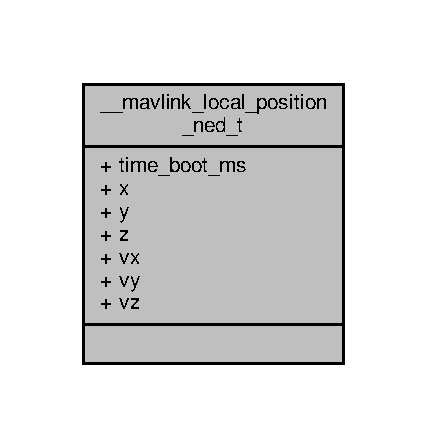
\includegraphics[width=205pt]{struct____mavlink__local__position__ned__t__coll__graph}
\end{center}
\end{figure}
\subsection*{Public Attributes}
\begin{DoxyCompactItemize}
\item 
\hypertarget{struct____mavlink__local__position__ned__t_a00187442905b1327719d9fde885a9bf9}{uint32\+\_\+t \hyperlink{struct____mavlink__local__position__ned__t_a00187442905b1327719d9fde885a9bf9}{time\+\_\+boot\+\_\+ms}}\label{struct____mavlink__local__position__ned__t_a00187442905b1327719d9fde885a9bf9}

\begin{DoxyCompactList}\small\item\em Timestamp (milliseconds since system boot) \end{DoxyCompactList}\item 
\hypertarget{struct____mavlink__local__position__ned__t_ab8f239110cba8ccc0f92aab56bc9a1d3}{float \hyperlink{struct____mavlink__local__position__ned__t_ab8f239110cba8ccc0f92aab56bc9a1d3}{x}}\label{struct____mavlink__local__position__ned__t_ab8f239110cba8ccc0f92aab56bc9a1d3}

\begin{DoxyCompactList}\small\item\em X Position. \end{DoxyCompactList}\item 
\hypertarget{struct____mavlink__local__position__ned__t_a56754cbe34638a9f6b5adca9ecf7fb44}{float \hyperlink{struct____mavlink__local__position__ned__t_a56754cbe34638a9f6b5adca9ecf7fb44}{y}}\label{struct____mavlink__local__position__ned__t_a56754cbe34638a9f6b5adca9ecf7fb44}

\begin{DoxyCompactList}\small\item\em Y Position. \end{DoxyCompactList}\item 
\hypertarget{struct____mavlink__local__position__ned__t_a4fc3fd6b6974b6b2356e4a7e28f9fecd}{float \hyperlink{struct____mavlink__local__position__ned__t_a4fc3fd6b6974b6b2356e4a7e28f9fecd}{z}}\label{struct____mavlink__local__position__ned__t_a4fc3fd6b6974b6b2356e4a7e28f9fecd}

\begin{DoxyCompactList}\small\item\em Z Position. \end{DoxyCompactList}\item 
\hypertarget{struct____mavlink__local__position__ned__t_a87216fec6527221da8812d77d8d84eb1}{float \hyperlink{struct____mavlink__local__position__ned__t_a87216fec6527221da8812d77d8d84eb1}{vx}}\label{struct____mavlink__local__position__ned__t_a87216fec6527221da8812d77d8d84eb1}

\begin{DoxyCompactList}\small\item\em X Speed. \end{DoxyCompactList}\item 
\hypertarget{struct____mavlink__local__position__ned__t_a0e9a5142819014e5807a657409608fa6}{float \hyperlink{struct____mavlink__local__position__ned__t_a0e9a5142819014e5807a657409608fa6}{vy}}\label{struct____mavlink__local__position__ned__t_a0e9a5142819014e5807a657409608fa6}

\begin{DoxyCompactList}\small\item\em Y Speed. \end{DoxyCompactList}\item 
\hypertarget{struct____mavlink__local__position__ned__t_aa34bbb949b0afd4bd524f455b9d980f6}{float \hyperlink{struct____mavlink__local__position__ned__t_aa34bbb949b0afd4bd524f455b9d980f6}{vz}}\label{struct____mavlink__local__position__ned__t_aa34bbb949b0afd4bd524f455b9d980f6}

\begin{DoxyCompactList}\small\item\em Z Speed. \end{DoxyCompactList}\end{DoxyCompactItemize}


The documentation for this struct was generated from the following file\+:\begin{DoxyCompactItemize}
\item 
/run/media/julien/\+Data/\+Documents/\+M\+A\+V\+R\+I\+C/\+M\+A\+V\+R\+I\+C\+\_\+\+Library/mavlink/include/common/mavlink\+\_\+msg\+\_\+local\+\_\+position\+\_\+ned.\+h\end{DoxyCompactItemize}

\hypertarget{struct____mavlink__local__position__setpoint__t}{\section{\+\_\+\+\_\+mavlink\+\_\+local\+\_\+position\+\_\+setpoint\+\_\+t Struct Reference}
\label{struct____mavlink__local__position__setpoint__t}\index{\+\_\+\+\_\+mavlink\+\_\+local\+\_\+position\+\_\+setpoint\+\_\+t@{\+\_\+\+\_\+mavlink\+\_\+local\+\_\+position\+\_\+setpoint\+\_\+t}}
}


Collaboration diagram for \+\_\+\+\_\+mavlink\+\_\+local\+\_\+position\+\_\+setpoint\+\_\+t\+:
\nopagebreak
\begin{figure}[H]
\begin{center}
\leavevmode
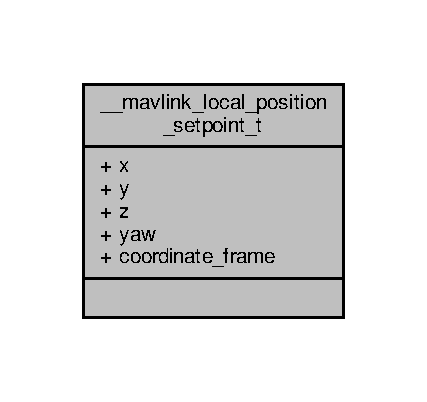
\includegraphics[width=205pt]{struct____mavlink__local__position__setpoint__t__coll__graph}
\end{center}
\end{figure}
\subsection*{Public Attributes}
\begin{DoxyCompactItemize}
\item 
\hypertarget{struct____mavlink__local__position__setpoint__t_a206e5fcf77dca173815edd4e9c5cfb2c}{float \hyperlink{struct____mavlink__local__position__setpoint__t_a206e5fcf77dca173815edd4e9c5cfb2c}{x}}\label{struct____mavlink__local__position__setpoint__t_a206e5fcf77dca173815edd4e9c5cfb2c}

\begin{DoxyCompactList}\small\item\em x position \end{DoxyCompactList}\item 
\hypertarget{struct____mavlink__local__position__setpoint__t_a99c553607e40da3cefd2d4221731c382}{float \hyperlink{struct____mavlink__local__position__setpoint__t_a99c553607e40da3cefd2d4221731c382}{y}}\label{struct____mavlink__local__position__setpoint__t_a99c553607e40da3cefd2d4221731c382}

\begin{DoxyCompactList}\small\item\em y position \end{DoxyCompactList}\item 
\hypertarget{struct____mavlink__local__position__setpoint__t_a3b95008f9ca33b3b1f0f23086dda34f2}{float \hyperlink{struct____mavlink__local__position__setpoint__t_a3b95008f9ca33b3b1f0f23086dda34f2}{z}}\label{struct____mavlink__local__position__setpoint__t_a3b95008f9ca33b3b1f0f23086dda34f2}

\begin{DoxyCompactList}\small\item\em z position \end{DoxyCompactList}\item 
\hypertarget{struct____mavlink__local__position__setpoint__t_a5fc83cf34d1de6841554d7413a9b3a86}{float \hyperlink{struct____mavlink__local__position__setpoint__t_a5fc83cf34d1de6841554d7413a9b3a86}{yaw}}\label{struct____mavlink__local__position__setpoint__t_a5fc83cf34d1de6841554d7413a9b3a86}

\begin{DoxyCompactList}\small\item\em Desired yaw angle. \end{DoxyCompactList}\item 
\hypertarget{struct____mavlink__local__position__setpoint__t_a1d1374da97eaf4caf6caa5fb431187ed}{uint8\+\_\+t \hyperlink{struct____mavlink__local__position__setpoint__t_a1d1374da97eaf4caf6caa5fb431187ed}{coordinate\+\_\+frame}}\label{struct____mavlink__local__position__setpoint__t_a1d1374da97eaf4caf6caa5fb431187ed}

\begin{DoxyCompactList}\small\item\em Coordinate frame -\/ valid values are only M\+A\+V\+\_\+\+F\+R\+A\+M\+E\+\_\+\+L\+O\+C\+A\+L\+\_\+\+N\+E\+D or M\+A\+V\+\_\+\+F\+R\+A\+M\+E\+\_\+\+L\+O\+C\+A\+L\+\_\+\+E\+N\+U. \end{DoxyCompactList}\end{DoxyCompactItemize}


The documentation for this struct was generated from the following file\+:\begin{DoxyCompactItemize}
\item 
/run/media/julien/\+Data/\+Documents/\+M\+A\+V\+R\+I\+C/\+M\+A\+V\+R\+I\+C\+\_\+\+Library/mavlink/include/common/mavlink\+\_\+msg\+\_\+local\+\_\+position\+\_\+setpoint.\+h\end{DoxyCompactItemize}

\hypertarget{struct____mavlink__manual__control__t}{\section{\+\_\+\+\_\+mavlink\+\_\+manual\+\_\+control\+\_\+t Struct Reference}
\label{struct____mavlink__manual__control__t}\index{\+\_\+\+\_\+mavlink\+\_\+manual\+\_\+control\+\_\+t@{\+\_\+\+\_\+mavlink\+\_\+manual\+\_\+control\+\_\+t}}
}


Collaboration diagram for \+\_\+\+\_\+mavlink\+\_\+manual\+\_\+control\+\_\+t\+:
\nopagebreak
\begin{figure}[H]
\begin{center}
\leavevmode
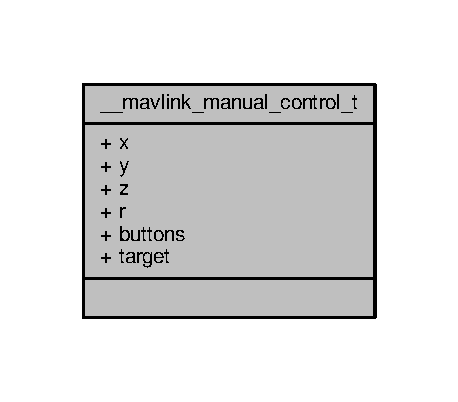
\includegraphics[width=220pt]{struct____mavlink__manual__control__t__coll__graph}
\end{center}
\end{figure}
\subsection*{Public Attributes}
\begin{DoxyCompactItemize}
\item 
\hypertarget{struct____mavlink__manual__control__t_add34b2bd0b54651701e7d8b2912868a6}{int16\+\_\+t \hyperlink{struct____mavlink__manual__control__t_add34b2bd0b54651701e7d8b2912868a6}{x}}\label{struct____mavlink__manual__control__t_add34b2bd0b54651701e7d8b2912868a6}

\begin{DoxyCompactList}\small\item\em X-\/axis, normalized to the range \mbox{[}-\/1000,1000\mbox{]}. A value of I\+N\+T16\+\_\+\+M\+A\+X indicates that this axis is invalid. Generally corresponds to forward(1000)-\/backward(-\/1000) movement on a joystick and the pitch of a vehicle. \end{DoxyCompactList}\item 
\hypertarget{struct____mavlink__manual__control__t_a5f705735ffdbe9c373151fe73c0abedb}{int16\+\_\+t \hyperlink{struct____mavlink__manual__control__t_a5f705735ffdbe9c373151fe73c0abedb}{y}}\label{struct____mavlink__manual__control__t_a5f705735ffdbe9c373151fe73c0abedb}

\begin{DoxyCompactList}\small\item\em Y-\/axis, normalized to the range \mbox{[}-\/1000,1000\mbox{]}. A value of I\+N\+T16\+\_\+\+M\+A\+X indicates that this axis is invalid. Generally corresponds to left(-\/1000)-\/right(1000) movement on a joystick and the roll of a vehicle. \end{DoxyCompactList}\item 
\hypertarget{struct____mavlink__manual__control__t_a9e3fd9d9bcd622e31cca4d44f66343c1}{int16\+\_\+t \hyperlink{struct____mavlink__manual__control__t_a9e3fd9d9bcd622e31cca4d44f66343c1}{z}}\label{struct____mavlink__manual__control__t_a9e3fd9d9bcd622e31cca4d44f66343c1}

\begin{DoxyCompactList}\small\item\em Z-\/axis, normalized to the range \mbox{[}-\/1000,1000\mbox{]}. A value of I\+N\+T16\+\_\+\+M\+A\+X indicates that this axis is invalid. Generally corresponds to a separate slider movement with maximum being 1000 and minimum being -\/1000 on a joystick and the thrust of a vehicle. \end{DoxyCompactList}\item 
\hypertarget{struct____mavlink__manual__control__t_a7311c5d986a66ba78c8f3c62e6163d8b}{int16\+\_\+t \hyperlink{struct____mavlink__manual__control__t_a7311c5d986a66ba78c8f3c62e6163d8b}{r}}\label{struct____mavlink__manual__control__t_a7311c5d986a66ba78c8f3c62e6163d8b}

\begin{DoxyCompactList}\small\item\em R-\/axis, normalized to the range \mbox{[}-\/1000,1000\mbox{]}. A value of I\+N\+T16\+\_\+\+M\+A\+X indicates that this axis is invalid. Generally corresponds to a twisting of the joystick, with counter-\/clockwise being 1000 and clockwise being -\/1000, and the yaw of a vehicle. \end{DoxyCompactList}\item 
\hypertarget{struct____mavlink__manual__control__t_addf991277abf6fad36b842fdba36fd89}{uint16\+\_\+t \hyperlink{struct____mavlink__manual__control__t_addf991277abf6fad36b842fdba36fd89}{buttons}}\label{struct____mavlink__manual__control__t_addf991277abf6fad36b842fdba36fd89}

\begin{DoxyCompactList}\small\item\em A bitfield corresponding to the joystick buttons' current state, 1 for pressed, 0 for released. The lowest bit corresponds to Button 1. \end{DoxyCompactList}\item 
\hypertarget{struct____mavlink__manual__control__t_ac69f96effc87ea6377989b2350a2a4eb}{uint8\+\_\+t \hyperlink{struct____mavlink__manual__control__t_ac69f96effc87ea6377989b2350a2a4eb}{target}}\label{struct____mavlink__manual__control__t_ac69f96effc87ea6377989b2350a2a4eb}

\begin{DoxyCompactList}\small\item\em The system to be controlled. \end{DoxyCompactList}\end{DoxyCompactItemize}


The documentation for this struct was generated from the following file\+:\begin{DoxyCompactItemize}
\item 
/run/media/julien/\+Data/\+Documents/\+M\+A\+V\+R\+I\+C/\+M\+A\+V\+R\+I\+C\+\_\+\+Library/mavlink/include/common/mavlink\+\_\+msg\+\_\+manual\+\_\+control.\+h\end{DoxyCompactItemize}

\hypertarget{struct____mavlink__manual__setpoint__t}{\section{\+\_\+\+\_\+mavlink\+\_\+manual\+\_\+setpoint\+\_\+t Struct Reference}
\label{struct____mavlink__manual__setpoint__t}\index{\+\_\+\+\_\+mavlink\+\_\+manual\+\_\+setpoint\+\_\+t@{\+\_\+\+\_\+mavlink\+\_\+manual\+\_\+setpoint\+\_\+t}}
}


Collaboration diagram for \+\_\+\+\_\+mavlink\+\_\+manual\+\_\+setpoint\+\_\+t\+:
\nopagebreak
\begin{figure}[H]
\begin{center}
\leavevmode
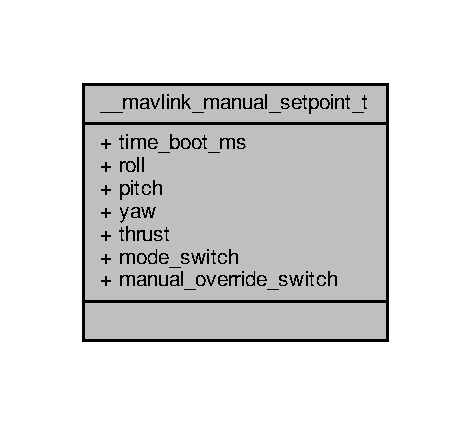
\includegraphics[width=226pt]{struct____mavlink__manual__setpoint__t__coll__graph}
\end{center}
\end{figure}
\subsection*{Public Attributes}
\begin{DoxyCompactItemize}
\item 
\hypertarget{struct____mavlink__manual__setpoint__t_aabfde5c1645ed2c5c0e3702cd3b7a63d}{uint32\+\_\+t \hyperlink{struct____mavlink__manual__setpoint__t_aabfde5c1645ed2c5c0e3702cd3b7a63d}{time\+\_\+boot\+\_\+ms}}\label{struct____mavlink__manual__setpoint__t_aabfde5c1645ed2c5c0e3702cd3b7a63d}

\begin{DoxyCompactList}\small\item\em Timestamp in milliseconds since system boot. \end{DoxyCompactList}\item 
\hypertarget{struct____mavlink__manual__setpoint__t_ab0fe1187926dd2bbdfb30c2bdbffbeaf}{float \hyperlink{struct____mavlink__manual__setpoint__t_ab0fe1187926dd2bbdfb30c2bdbffbeaf}{roll}}\label{struct____mavlink__manual__setpoint__t_ab0fe1187926dd2bbdfb30c2bdbffbeaf}

\begin{DoxyCompactList}\small\item\em Desired roll rate in radians per second. \end{DoxyCompactList}\item 
\hypertarget{struct____mavlink__manual__setpoint__t_a17e3f9bb6707394163aafdbf02539694}{float \hyperlink{struct____mavlink__manual__setpoint__t_a17e3f9bb6707394163aafdbf02539694}{pitch}}\label{struct____mavlink__manual__setpoint__t_a17e3f9bb6707394163aafdbf02539694}

\begin{DoxyCompactList}\small\item\em Desired pitch rate in radians per second. \end{DoxyCompactList}\item 
\hypertarget{struct____mavlink__manual__setpoint__t_ab3e21184ffcf6b5451f8227d6ccb35bc}{float \hyperlink{struct____mavlink__manual__setpoint__t_ab3e21184ffcf6b5451f8227d6ccb35bc}{yaw}}\label{struct____mavlink__manual__setpoint__t_ab3e21184ffcf6b5451f8227d6ccb35bc}

\begin{DoxyCompactList}\small\item\em Desired yaw rate in radians per second. \end{DoxyCompactList}\item 
\hypertarget{struct____mavlink__manual__setpoint__t_a2044f740a7e79365a9edf603e5c29d3c}{float \hyperlink{struct____mavlink__manual__setpoint__t_a2044f740a7e79365a9edf603e5c29d3c}{thrust}}\label{struct____mavlink__manual__setpoint__t_a2044f740a7e79365a9edf603e5c29d3c}

\begin{DoxyCompactList}\small\item\em Collective thrust, normalized to 0 .. 1. \end{DoxyCompactList}\item 
\hypertarget{struct____mavlink__manual__setpoint__t_ac3e1509a46421fac372fc2e917b85c1c}{uint8\+\_\+t \hyperlink{struct____mavlink__manual__setpoint__t_ac3e1509a46421fac372fc2e917b85c1c}{mode\+\_\+switch}}\label{struct____mavlink__manual__setpoint__t_ac3e1509a46421fac372fc2e917b85c1c}

\begin{DoxyCompactList}\small\item\em Flight mode switch position, 0.. 255. \end{DoxyCompactList}\item 
\hypertarget{struct____mavlink__manual__setpoint__t_ac32326ac4f3f6983bfc36717d432643f}{uint8\+\_\+t \hyperlink{struct____mavlink__manual__setpoint__t_ac32326ac4f3f6983bfc36717d432643f}{manual\+\_\+override\+\_\+switch}}\label{struct____mavlink__manual__setpoint__t_ac32326ac4f3f6983bfc36717d432643f}

\begin{DoxyCompactList}\small\item\em Override mode switch position, 0.. 255. \end{DoxyCompactList}\end{DoxyCompactItemize}


The documentation for this struct was generated from the following file\+:\begin{DoxyCompactItemize}
\item 
/run/media/julien/\+Data/\+Documents/\+M\+A\+V\+R\+I\+C/\+M\+A\+V\+R\+I\+C\+\_\+\+Library/mavlink/include/common/mavlink\+\_\+msg\+\_\+manual\+\_\+setpoint.\+h\end{DoxyCompactItemize}

\hypertarget{struct____mavlink__memory__vect__t}{\section{\+\_\+\+\_\+mavlink\+\_\+memory\+\_\+vect\+\_\+t Struct Reference}
\label{struct____mavlink__memory__vect__t}\index{\+\_\+\+\_\+mavlink\+\_\+memory\+\_\+vect\+\_\+t@{\+\_\+\+\_\+mavlink\+\_\+memory\+\_\+vect\+\_\+t}}
}


Collaboration diagram for \+\_\+\+\_\+mavlink\+\_\+memory\+\_\+vect\+\_\+t\+:
\nopagebreak
\begin{figure}[H]
\begin{center}
\leavevmode
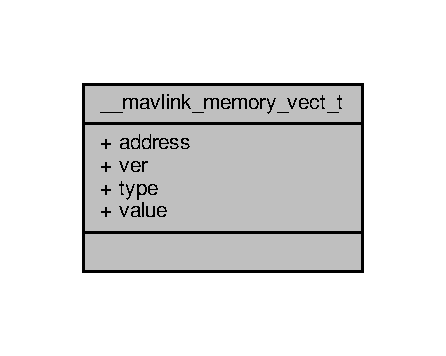
\includegraphics[width=214pt]{struct____mavlink__memory__vect__t__coll__graph}
\end{center}
\end{figure}
\subsection*{Public Attributes}
\begin{DoxyCompactItemize}
\item 
\hypertarget{struct____mavlink__memory__vect__t_a079a0cecfd6f6e3d47c4c1d324ddd29d}{uint16\+\_\+t \hyperlink{struct____mavlink__memory__vect__t_a079a0cecfd6f6e3d47c4c1d324ddd29d}{address}}\label{struct____mavlink__memory__vect__t_a079a0cecfd6f6e3d47c4c1d324ddd29d}

\begin{DoxyCompactList}\small\item\em Starting address of the debug variables. \end{DoxyCompactList}\item 
\hypertarget{struct____mavlink__memory__vect__t_acb180cded1d3dcbf3e719545b50f392e}{uint8\+\_\+t \hyperlink{struct____mavlink__memory__vect__t_acb180cded1d3dcbf3e719545b50f392e}{ver}}\label{struct____mavlink__memory__vect__t_acb180cded1d3dcbf3e719545b50f392e}

\begin{DoxyCompactList}\small\item\em Version code of the type variable. 0=unknown, type ignored and assumed int16\+\_\+t. 1=as below. \end{DoxyCompactList}\item 
\hypertarget{struct____mavlink__memory__vect__t_a5c37b4f5d396209693c7bb32097a6e88}{uint8\+\_\+t \hyperlink{struct____mavlink__memory__vect__t_a5c37b4f5d396209693c7bb32097a6e88}{type}}\label{struct____mavlink__memory__vect__t_a5c37b4f5d396209693c7bb32097a6e88}

\begin{DoxyCompactList}\small\item\em Type code of the memory variables. for ver = 1\+: 0=16 x int16\+\_\+t, 1=16 x uint16\+\_\+t, 2=16 x Q15, 3=16 x 1\+Q14. \end{DoxyCompactList}\item 
\hypertarget{struct____mavlink__memory__vect__t_aa4c3207a3dbc0e0a3b821b90740ad4e6}{int8\+\_\+t \hyperlink{struct____mavlink__memory__vect__t_aa4c3207a3dbc0e0a3b821b90740ad4e6}{value} \mbox{[}32\mbox{]}}\label{struct____mavlink__memory__vect__t_aa4c3207a3dbc0e0a3b821b90740ad4e6}

\begin{DoxyCompactList}\small\item\em Memory contents at specified address. \end{DoxyCompactList}\end{DoxyCompactItemize}


The documentation for this struct was generated from the following file\+:\begin{DoxyCompactItemize}
\item 
/run/media/julien/\+Data/\+Documents/\+M\+A\+V\+R\+I\+C/\+M\+A\+V\+R\+I\+C\+\_\+\+Library/mavlink/include/common/mavlink\+\_\+msg\+\_\+memory\+\_\+vect.\+h\end{DoxyCompactItemize}

\hypertarget{struct____mavlink__message}{\section{\+\_\+\+\_\+mavlink\+\_\+message Struct Reference}
\label{struct____mavlink__message}\index{\+\_\+\+\_\+mavlink\+\_\+message@{\+\_\+\+\_\+mavlink\+\_\+message}}
}


Collaboration diagram for \+\_\+\+\_\+mavlink\+\_\+message\+:
\nopagebreak
\begin{figure}[H]
\begin{center}
\leavevmode
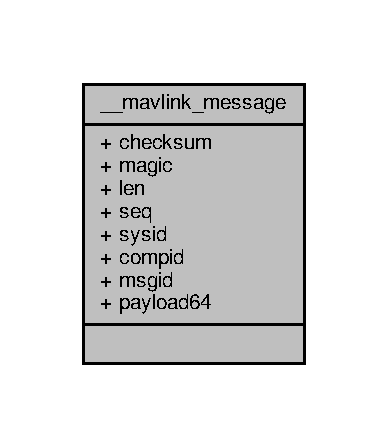
\includegraphics[width=186pt]{struct____mavlink__message__coll__graph}
\end{center}
\end{figure}
\subsection*{Public Attributes}
\begin{DoxyCompactItemize}
\item 
\hypertarget{struct____mavlink__message_a8c200d7751471b5ac54d090ba279a5a6}{uint16\+\_\+t {\bfseries checksum}}\label{struct____mavlink__message_a8c200d7751471b5ac54d090ba279a5a6}

\item 
uint8\+\_\+t \hyperlink{struct____mavlink__message_a2e6ee9d46821aea33a08231dea000355}{magic}
\begin{DoxyCompactList}\small\item\em sent at end of packet \end{DoxyCompactList}\item 
\hypertarget{struct____mavlink__message_a6a405c678e4b9fe57e5e621c5bcd4841}{uint8\+\_\+t \hyperlink{struct____mavlink__message_a6a405c678e4b9fe57e5e621c5bcd4841}{len}}\label{struct____mavlink__message_a6a405c678e4b9fe57e5e621c5bcd4841}

\begin{DoxyCompactList}\small\item\em Length of payload. \end{DoxyCompactList}\item 
\hypertarget{struct____mavlink__message_aae05bedaab3c62acaccb416478490eff}{uint8\+\_\+t \hyperlink{struct____mavlink__message_aae05bedaab3c62acaccb416478490eff}{seq}}\label{struct____mavlink__message_aae05bedaab3c62acaccb416478490eff}

\begin{DoxyCompactList}\small\item\em Sequence of packet. \end{DoxyCompactList}\item 
\hypertarget{struct____mavlink__message_ad4bfd4108688429b30940a35b44d4dd3}{uint8\+\_\+t \hyperlink{struct____mavlink__message_ad4bfd4108688429b30940a35b44d4dd3}{sysid}}\label{struct____mavlink__message_ad4bfd4108688429b30940a35b44d4dd3}

\begin{DoxyCompactList}\small\item\em I\+D of message sender system/aircraft. \end{DoxyCompactList}\item 
\hypertarget{struct____mavlink__message_a83ed773c359ffe4a8d0746f82af2b44d}{uint8\+\_\+t \hyperlink{struct____mavlink__message_a83ed773c359ffe4a8d0746f82af2b44d}{compid}}\label{struct____mavlink__message_a83ed773c359ffe4a8d0746f82af2b44d}

\begin{DoxyCompactList}\small\item\em I\+D of the message sender component. \end{DoxyCompactList}\item 
\hypertarget{struct____mavlink__message_a8d95b61c61b9086bada158104828d593}{uint8\+\_\+t \hyperlink{struct____mavlink__message_a8d95b61c61b9086bada158104828d593}{msgid}}\label{struct____mavlink__message_a8d95b61c61b9086bada158104828d593}

\begin{DoxyCompactList}\small\item\em I\+D of message in payload. \end{DoxyCompactList}\item 
\hypertarget{struct____mavlink__message_a267401209e74271b7ded879bb0f44e73}{uint64\+\_\+t {\bfseries payload64} \mbox{[}(M\+A\+V\+L\+I\+N\+K\+\_\+\+M\+A\+X\+\_\+\+P\+A\+Y\+L\+O\+A\+D\+\_\+\+L\+E\+N+M\+A\+V\+L\+I\+N\+K\+\_\+\+N\+U\+M\+\_\+\+C\+H\+E\+C\+K\+S\+U\+M\+\_\+\+B\+Y\+T\+E\+S+7)/8\mbox{]}}\label{struct____mavlink__message_a267401209e74271b7ded879bb0f44e73}

\end{DoxyCompactItemize}


\subsection{Member Data Documentation}
\hypertarget{struct____mavlink__message_a2e6ee9d46821aea33a08231dea000355}{\index{\+\_\+\+\_\+mavlink\+\_\+message@{\+\_\+\+\_\+mavlink\+\_\+message}!magic@{magic}}
\index{magic@{magic}!\+\_\+\+\_\+mavlink\+\_\+message@{\+\_\+\+\_\+mavlink\+\_\+message}}
\subsubsection[{magic}]{\setlength{\rightskip}{0pt plus 5cm}uint8\+\_\+t \+\_\+\+\_\+mavlink\+\_\+message\+::magic}}\label{struct____mavlink__message_a2e6ee9d46821aea33a08231dea000355}


sent at end of packet 

protocol magic marker 

The documentation for this struct was generated from the following file\+:\begin{DoxyCompactItemize}
\item 
/run/media/julien/\+Data/\+Documents/\+M\+A\+V\+R\+I\+C/\+M\+A\+V\+R\+I\+C\+\_\+\+Library/mavlink/include/mavlink\+\_\+types.\+h\end{DoxyCompactItemize}

\hypertarget{struct____mavlink__message__info}{\section{\+\_\+\+\_\+mavlink\+\_\+message\+\_\+info Struct Reference}
\label{struct____mavlink__message__info}\index{\+\_\+\+\_\+mavlink\+\_\+message\+\_\+info@{\+\_\+\+\_\+mavlink\+\_\+message\+\_\+info}}
}


Collaboration diagram for \+\_\+\+\_\+mavlink\+\_\+message\+\_\+info\+:
\nopagebreak
\begin{figure}[H]
\begin{center}
\leavevmode
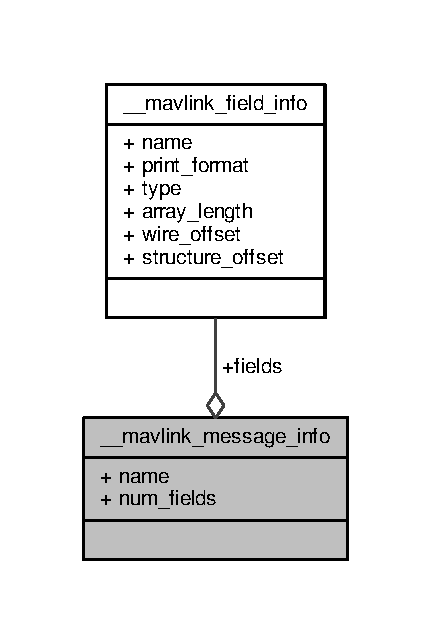
\includegraphics[width=207pt]{struct____mavlink__message__info__coll__graph}
\end{center}
\end{figure}
\subsection*{Public Attributes}
\begin{DoxyCompactItemize}
\item 
\hypertarget{struct____mavlink__message__info_a5e8b48c51cb8bc44bd844d1c3049ee32}{const char $\ast$ {\bfseries name}}\label{struct____mavlink__message__info_a5e8b48c51cb8bc44bd844d1c3049ee32}

\item 
\hypertarget{struct____mavlink__message__info_a0c343bcc1f27884e8c2ab875e7efc2e5}{unsigned {\bfseries num\+\_\+fields}}\label{struct____mavlink__message__info_a0c343bcc1f27884e8c2ab875e7efc2e5}

\item 
\hypertarget{struct____mavlink__message__info_a4a15f20958b43cb1282575c6da67a37b}{\hyperlink{struct____mavlink__field__info}{mavlink\+\_\+field\+\_\+info\+\_\+t} {\bfseries fields} \mbox{[}M\+A\+V\+L\+I\+N\+K\+\_\+\+M\+A\+X\+\_\+\+F\+I\+E\+L\+D\+S\mbox{]}}\label{struct____mavlink__message__info_a4a15f20958b43cb1282575c6da67a37b}

\end{DoxyCompactItemize}


The documentation for this struct was generated from the following file\+:\begin{DoxyCompactItemize}
\item 
/run/media/julien/\+Data/\+Documents/\+M\+A\+V\+R\+I\+C/\+M\+A\+V\+R\+I\+C\+\_\+\+Library/mavlink/include/mavlink\+\_\+types.\+h\end{DoxyCompactItemize}

\hypertarget{struct____mavlink__mission__ack__t}{\section{\+\_\+\+\_\+mavlink\+\_\+mission\+\_\+ack\+\_\+t Struct Reference}
\label{struct____mavlink__mission__ack__t}\index{\+\_\+\+\_\+mavlink\+\_\+mission\+\_\+ack\+\_\+t@{\+\_\+\+\_\+mavlink\+\_\+mission\+\_\+ack\+\_\+t}}
}


Collaboration diagram for \+\_\+\+\_\+mavlink\+\_\+mission\+\_\+ack\+\_\+t\+:
\nopagebreak
\begin{figure}[H]
\begin{center}
\leavevmode
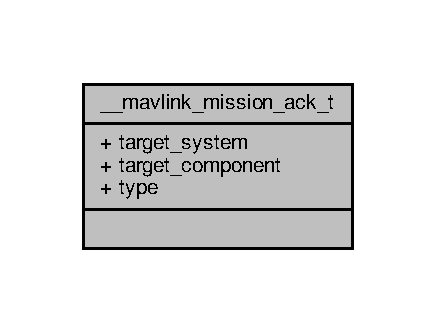
\includegraphics[width=209pt]{struct____mavlink__mission__ack__t__coll__graph}
\end{center}
\end{figure}
\subsection*{Public Attributes}
\begin{DoxyCompactItemize}
\item 
\hypertarget{struct____mavlink__mission__ack__t_ab8ef2eb9bff8975de92406b94c18d907}{uint8\+\_\+t \hyperlink{struct____mavlink__mission__ack__t_ab8ef2eb9bff8975de92406b94c18d907}{target\+\_\+system}}\label{struct____mavlink__mission__ack__t_ab8ef2eb9bff8975de92406b94c18d907}

\begin{DoxyCompactList}\small\item\em System I\+D. \end{DoxyCompactList}\item 
\hypertarget{struct____mavlink__mission__ack__t_ab254af31fbc3e92ab8cffcea8bd78fba}{uint8\+\_\+t \hyperlink{struct____mavlink__mission__ack__t_ab254af31fbc3e92ab8cffcea8bd78fba}{target\+\_\+component}}\label{struct____mavlink__mission__ack__t_ab254af31fbc3e92ab8cffcea8bd78fba}

\begin{DoxyCompactList}\small\item\em Component I\+D. \end{DoxyCompactList}\item 
\hypertarget{struct____mavlink__mission__ack__t_ad05f998d3b1bea0480eb25dcb82e0c92}{uint8\+\_\+t \hyperlink{struct____mavlink__mission__ack__t_ad05f998d3b1bea0480eb25dcb82e0c92}{type}}\label{struct____mavlink__mission__ack__t_ad05f998d3b1bea0480eb25dcb82e0c92}

\begin{DoxyCompactList}\small\item\em See M\+A\+V\+\_\+\+M\+I\+S\+S\+I\+O\+N\+\_\+\+R\+E\+S\+U\+L\+T enum. \end{DoxyCompactList}\end{DoxyCompactItemize}


The documentation for this struct was generated from the following file\+:\begin{DoxyCompactItemize}
\item 
/run/media/julien/\+Data/\+Documents/\+M\+A\+V\+R\+I\+C/\+M\+A\+V\+R\+I\+C\+\_\+\+Library/mavlink/include/common/mavlink\+\_\+msg\+\_\+mission\+\_\+ack.\+h\end{DoxyCompactItemize}

\hypertarget{struct____mavlink__mission__clear__all__t}{\section{\+\_\+\+\_\+mavlink\+\_\+mission\+\_\+clear\+\_\+all\+\_\+t Struct Reference}
\label{struct____mavlink__mission__clear__all__t}\index{\+\_\+\+\_\+mavlink\+\_\+mission\+\_\+clear\+\_\+all\+\_\+t@{\+\_\+\+\_\+mavlink\+\_\+mission\+\_\+clear\+\_\+all\+\_\+t}}
}


Collaboration diagram for \+\_\+\+\_\+mavlink\+\_\+mission\+\_\+clear\+\_\+all\+\_\+t\+:
\nopagebreak
\begin{figure}[H]
\begin{center}
\leavevmode
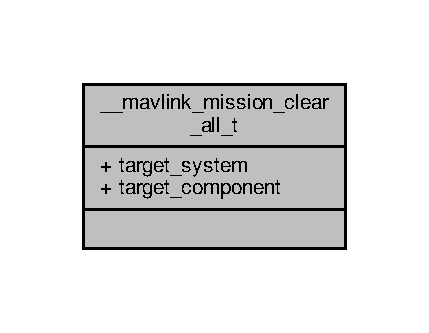
\includegraphics[width=206pt]{struct____mavlink__mission__clear__all__t__coll__graph}
\end{center}
\end{figure}
\subsection*{Public Attributes}
\begin{DoxyCompactItemize}
\item 
\hypertarget{struct____mavlink__mission__clear__all__t_ad628d39e2e099c3c1c015b15b7d4d150}{uint8\+\_\+t \hyperlink{struct____mavlink__mission__clear__all__t_ad628d39e2e099c3c1c015b15b7d4d150}{target\+\_\+system}}\label{struct____mavlink__mission__clear__all__t_ad628d39e2e099c3c1c015b15b7d4d150}

\begin{DoxyCompactList}\small\item\em System I\+D. \end{DoxyCompactList}\item 
\hypertarget{struct____mavlink__mission__clear__all__t_ac3e8927334773420a64fcd60202651f1}{uint8\+\_\+t \hyperlink{struct____mavlink__mission__clear__all__t_ac3e8927334773420a64fcd60202651f1}{target\+\_\+component}}\label{struct____mavlink__mission__clear__all__t_ac3e8927334773420a64fcd60202651f1}

\begin{DoxyCompactList}\small\item\em Component I\+D. \end{DoxyCompactList}\end{DoxyCompactItemize}


The documentation for this struct was generated from the following file\+:\begin{DoxyCompactItemize}
\item 
/run/media/julien/\+Data/\+Documents/\+M\+A\+V\+R\+I\+C/\+M\+A\+V\+R\+I\+C\+\_\+\+Library/mavlink/include/common/mavlink\+\_\+msg\+\_\+mission\+\_\+clear\+\_\+all.\+h\end{DoxyCompactItemize}

\hypertarget{struct____mavlink__mission__count__t}{\section{\+\_\+\+\_\+mavlink\+\_\+mission\+\_\+count\+\_\+t Struct Reference}
\label{struct____mavlink__mission__count__t}\index{\+\_\+\+\_\+mavlink\+\_\+mission\+\_\+count\+\_\+t@{\+\_\+\+\_\+mavlink\+\_\+mission\+\_\+count\+\_\+t}}
}


Collaboration diagram for \+\_\+\+\_\+mavlink\+\_\+mission\+\_\+count\+\_\+t\+:
\nopagebreak
\begin{figure}[H]
\begin{center}
\leavevmode
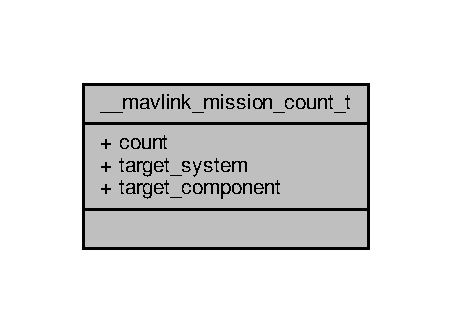
\includegraphics[width=217pt]{struct____mavlink__mission__count__t__coll__graph}
\end{center}
\end{figure}
\subsection*{Public Attributes}
\begin{DoxyCompactItemize}
\item 
\hypertarget{struct____mavlink__mission__count__t_ae0f07b1c9ffca95b6c76cde724eda5d9}{uint16\+\_\+t \hyperlink{struct____mavlink__mission__count__t_ae0f07b1c9ffca95b6c76cde724eda5d9}{count}}\label{struct____mavlink__mission__count__t_ae0f07b1c9ffca95b6c76cde724eda5d9}

\begin{DoxyCompactList}\small\item\em Number of mission items in the sequence. \end{DoxyCompactList}\item 
\hypertarget{struct____mavlink__mission__count__t_a9e211af96b9dd62f71c32fb3412dbfca}{uint8\+\_\+t \hyperlink{struct____mavlink__mission__count__t_a9e211af96b9dd62f71c32fb3412dbfca}{target\+\_\+system}}\label{struct____mavlink__mission__count__t_a9e211af96b9dd62f71c32fb3412dbfca}

\begin{DoxyCompactList}\small\item\em System I\+D. \end{DoxyCompactList}\item 
\hypertarget{struct____mavlink__mission__count__t_a21576207ae6595d5272a405fb8c198bf}{uint8\+\_\+t \hyperlink{struct____mavlink__mission__count__t_a21576207ae6595d5272a405fb8c198bf}{target\+\_\+component}}\label{struct____mavlink__mission__count__t_a21576207ae6595d5272a405fb8c198bf}

\begin{DoxyCompactList}\small\item\em Component I\+D. \end{DoxyCompactList}\end{DoxyCompactItemize}


The documentation for this struct was generated from the following file\+:\begin{DoxyCompactItemize}
\item 
/run/media/julien/\+Data/\+Documents/\+M\+A\+V\+R\+I\+C/\+M\+A\+V\+R\+I\+C\+\_\+\+Library/mavlink/include/common/mavlink\+\_\+msg\+\_\+mission\+\_\+count.\+h\end{DoxyCompactItemize}

\hypertarget{struct____mavlink__mission__current__t}{\section{\+\_\+\+\_\+mavlink\+\_\+mission\+\_\+current\+\_\+t Struct Reference}
\label{struct____mavlink__mission__current__t}\index{\+\_\+\+\_\+mavlink\+\_\+mission\+\_\+current\+\_\+t@{\+\_\+\+\_\+mavlink\+\_\+mission\+\_\+current\+\_\+t}}
}


Collaboration diagram for \+\_\+\+\_\+mavlink\+\_\+mission\+\_\+current\+\_\+t\+:
\nopagebreak
\begin{figure}[H]
\begin{center}
\leavevmode
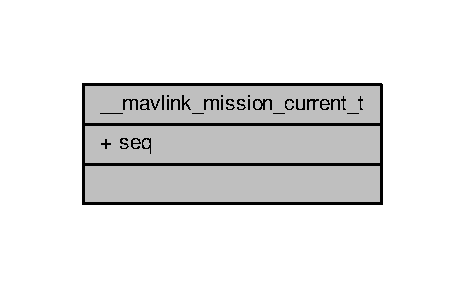
\includegraphics[width=223pt]{struct____mavlink__mission__current__t__coll__graph}
\end{center}
\end{figure}
\subsection*{Public Attributes}
\begin{DoxyCompactItemize}
\item 
\hypertarget{struct____mavlink__mission__current__t_abf05ebfb452002e779838949ae335023}{uint16\+\_\+t \hyperlink{struct____mavlink__mission__current__t_abf05ebfb452002e779838949ae335023}{seq}}\label{struct____mavlink__mission__current__t_abf05ebfb452002e779838949ae335023}

\begin{DoxyCompactList}\small\item\em Sequence. \end{DoxyCompactList}\end{DoxyCompactItemize}


The documentation for this struct was generated from the following file\+:\begin{DoxyCompactItemize}
\item 
/run/media/julien/\+Data/\+Documents/\+M\+A\+V\+R\+I\+C/\+M\+A\+V\+R\+I\+C\+\_\+\+Library/mavlink/include/common/mavlink\+\_\+msg\+\_\+mission\+\_\+current.\+h\end{DoxyCompactItemize}

\hypertarget{struct____mavlink__mission__item__reached__t}{\section{\+\_\+\+\_\+mavlink\+\_\+mission\+\_\+item\+\_\+reached\+\_\+t Struct Reference}
\label{struct____mavlink__mission__item__reached__t}\index{\+\_\+\+\_\+mavlink\+\_\+mission\+\_\+item\+\_\+reached\+\_\+t@{\+\_\+\+\_\+mavlink\+\_\+mission\+\_\+item\+\_\+reached\+\_\+t}}
}


Collaboration diagram for \+\_\+\+\_\+mavlink\+\_\+mission\+\_\+item\+\_\+reached\+\_\+t\+:
\nopagebreak
\begin{figure}[H]
\begin{center}
\leavevmode
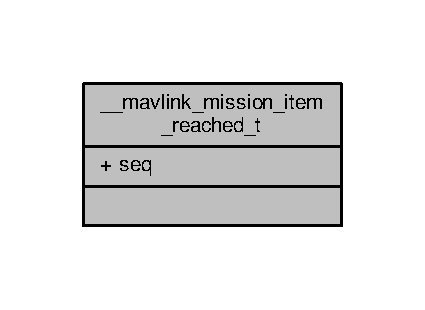
\includegraphics[width=204pt]{struct____mavlink__mission__item__reached__t__coll__graph}
\end{center}
\end{figure}
\subsection*{Public Attributes}
\begin{DoxyCompactItemize}
\item 
\hypertarget{struct____mavlink__mission__item__reached__t_acdab74a4633c0c3b3dfcfa75c9d2b234}{uint16\+\_\+t \hyperlink{struct____mavlink__mission__item__reached__t_acdab74a4633c0c3b3dfcfa75c9d2b234}{seq}}\label{struct____mavlink__mission__item__reached__t_acdab74a4633c0c3b3dfcfa75c9d2b234}

\begin{DoxyCompactList}\small\item\em Sequence. \end{DoxyCompactList}\end{DoxyCompactItemize}


The documentation for this struct was generated from the following file\+:\begin{DoxyCompactItemize}
\item 
/run/media/julien/\+Data/\+Documents/\+M\+A\+V\+R\+I\+C/\+M\+A\+V\+R\+I\+C\+\_\+\+Library/mavlink/include/common/mavlink\+\_\+msg\+\_\+mission\+\_\+item\+\_\+reached.\+h\end{DoxyCompactItemize}

\hypertarget{struct____mavlink__mission__item__t}{\section{\+\_\+\+\_\+mavlink\+\_\+mission\+\_\+item\+\_\+t Struct Reference}
\label{struct____mavlink__mission__item__t}\index{\+\_\+\+\_\+mavlink\+\_\+mission\+\_\+item\+\_\+t@{\+\_\+\+\_\+mavlink\+\_\+mission\+\_\+item\+\_\+t}}
}


Collaboration diagram for \+\_\+\+\_\+mavlink\+\_\+mission\+\_\+item\+\_\+t\+:
\nopagebreak
\begin{figure}[H]
\begin{center}
\leavevmode
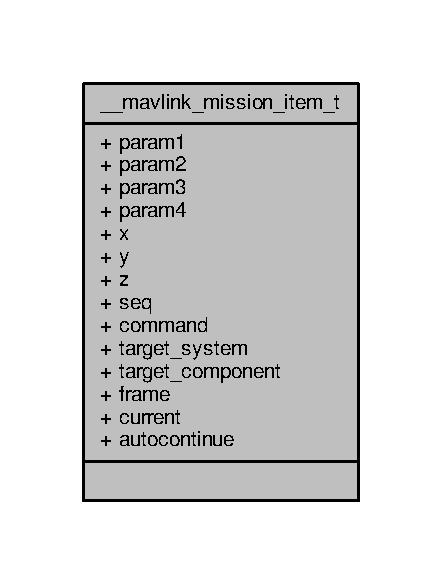
\includegraphics[width=212pt]{struct____mavlink__mission__item__t__coll__graph}
\end{center}
\end{figure}
\subsection*{Public Attributes}
\begin{DoxyCompactItemize}
\item 
\hypertarget{struct____mavlink__mission__item__t_a7b622b789be829088a8c9353946a4f28}{float \hyperlink{struct____mavlink__mission__item__t_a7b622b789be829088a8c9353946a4f28}{param1}}\label{struct____mavlink__mission__item__t_a7b622b789be829088a8c9353946a4f28}

\begin{DoxyCompactList}\small\item\em P\+A\+R\+A\+M1 / For N\+A\+V command M\+I\+S\+S\+I\+O\+Ns\+: Radius in which the M\+I\+S\+S\+I\+O\+N is accepted as reached, in meters. \end{DoxyCompactList}\item 
\hypertarget{struct____mavlink__mission__item__t_ad523243067b6c47919554e8802f14b5c}{float \hyperlink{struct____mavlink__mission__item__t_ad523243067b6c47919554e8802f14b5c}{param2}}\label{struct____mavlink__mission__item__t_ad523243067b6c47919554e8802f14b5c}

\begin{DoxyCompactList}\small\item\em P\+A\+R\+A\+M2 / For N\+A\+V command M\+I\+S\+S\+I\+O\+Ns\+: Time that the M\+A\+V should stay inside the P\+A\+R\+A\+M1 radius before advancing, in milliseconds. \end{DoxyCompactList}\item 
\hypertarget{struct____mavlink__mission__item__t_a183425d5376a9173373279cc43ffce25}{float \hyperlink{struct____mavlink__mission__item__t_a183425d5376a9173373279cc43ffce25}{param3}}\label{struct____mavlink__mission__item__t_a183425d5376a9173373279cc43ffce25}

\begin{DoxyCompactList}\small\item\em P\+A\+R\+A\+M3 / For L\+O\+I\+T\+E\+R command M\+I\+S\+S\+I\+O\+Ns\+: Orbit to circle around the M\+I\+S\+S\+I\+O\+N, in meters. If positive the orbit direction should be clockwise, if negative the orbit direction should be counter-\/clockwise. \end{DoxyCompactList}\item 
\hypertarget{struct____mavlink__mission__item__t_a8db8965269e5523972f4645f9b52d86d}{float \hyperlink{struct____mavlink__mission__item__t_a8db8965269e5523972f4645f9b52d86d}{param4}}\label{struct____mavlink__mission__item__t_a8db8965269e5523972f4645f9b52d86d}

\begin{DoxyCompactList}\small\item\em P\+A\+R\+A\+M4 / For N\+A\+V and L\+O\+I\+T\+E\+R command M\+I\+S\+S\+I\+O\+Ns\+: Yaw orientation in degrees, \mbox{[}0..360\mbox{]} 0 = N\+O\+R\+T\+H. \end{DoxyCompactList}\item 
\hypertarget{struct____mavlink__mission__item__t_a578c43dbf85decd47437180c89407f93}{float \hyperlink{struct____mavlink__mission__item__t_a578c43dbf85decd47437180c89407f93}{x}}\label{struct____mavlink__mission__item__t_a578c43dbf85decd47437180c89407f93}

\begin{DoxyCompactList}\small\item\em P\+A\+R\+A\+M5 / local\+: x position, global\+: latitude. \end{DoxyCompactList}\item 
\hypertarget{struct____mavlink__mission__item__t_a916e8ea61a94ce7b854ebd11cc5eea37}{float \hyperlink{struct____mavlink__mission__item__t_a916e8ea61a94ce7b854ebd11cc5eea37}{y}}\label{struct____mavlink__mission__item__t_a916e8ea61a94ce7b854ebd11cc5eea37}

\begin{DoxyCompactList}\small\item\em P\+A\+R\+A\+M6 / y position\+: global\+: longitude. \end{DoxyCompactList}\item 
\hypertarget{struct____mavlink__mission__item__t_adfa6844101b755c5e439b46f21ba0be8}{float \hyperlink{struct____mavlink__mission__item__t_adfa6844101b755c5e439b46f21ba0be8}{z}}\label{struct____mavlink__mission__item__t_adfa6844101b755c5e439b46f21ba0be8}

\begin{DoxyCompactList}\small\item\em P\+A\+R\+A\+M7 / z position\+: global\+: altitude. \end{DoxyCompactList}\item 
\hypertarget{struct____mavlink__mission__item__t_a0038a8dc2e0dc3757272b160a0cbaac2}{uint16\+\_\+t \hyperlink{struct____mavlink__mission__item__t_a0038a8dc2e0dc3757272b160a0cbaac2}{seq}}\label{struct____mavlink__mission__item__t_a0038a8dc2e0dc3757272b160a0cbaac2}

\begin{DoxyCompactList}\small\item\em Sequence. \end{DoxyCompactList}\item 
\hypertarget{struct____mavlink__mission__item__t_ad5a94a67caa147049e45c3754f15daa7}{uint16\+\_\+t \hyperlink{struct____mavlink__mission__item__t_ad5a94a67caa147049e45c3754f15daa7}{command}}\label{struct____mavlink__mission__item__t_ad5a94a67caa147049e45c3754f15daa7}

\begin{DoxyCompactList}\small\item\em The scheduled action for the M\+I\+S\+S\+I\+O\+N. see M\+A\+V\+\_\+\+C\+M\+D in common.\+xml M\+A\+V\+Link specs. \end{DoxyCompactList}\item 
\hypertarget{struct____mavlink__mission__item__t_ab6e5076aa5f0e524e88879bebf0ed483}{uint8\+\_\+t \hyperlink{struct____mavlink__mission__item__t_ab6e5076aa5f0e524e88879bebf0ed483}{target\+\_\+system}}\label{struct____mavlink__mission__item__t_ab6e5076aa5f0e524e88879bebf0ed483}

\begin{DoxyCompactList}\small\item\em System I\+D. \end{DoxyCompactList}\item 
\hypertarget{struct____mavlink__mission__item__t_a6bb8183ef3416741edca46337e6e6860}{uint8\+\_\+t \hyperlink{struct____mavlink__mission__item__t_a6bb8183ef3416741edca46337e6e6860}{target\+\_\+component}}\label{struct____mavlink__mission__item__t_a6bb8183ef3416741edca46337e6e6860}

\begin{DoxyCompactList}\small\item\em Component I\+D. \end{DoxyCompactList}\item 
\hypertarget{struct____mavlink__mission__item__t_aa3b25a65ef4d62f208ea6d3856b418cb}{uint8\+\_\+t \hyperlink{struct____mavlink__mission__item__t_aa3b25a65ef4d62f208ea6d3856b418cb}{frame}}\label{struct____mavlink__mission__item__t_aa3b25a65ef4d62f208ea6d3856b418cb}

\begin{DoxyCompactList}\small\item\em The coordinate system of the M\+I\+S\+S\+I\+O\+N. see M\+A\+V\+\_\+\+F\+R\+A\+M\+E in \hyperlink{mavlink__types_8h_source}{mavlink\+\_\+types.\+h}. \end{DoxyCompactList}\item 
\hypertarget{struct____mavlink__mission__item__t_aa9fdaa647214fcb6bb21e05f2718f56f}{uint8\+\_\+t \hyperlink{struct____mavlink__mission__item__t_aa9fdaa647214fcb6bb21e05f2718f56f}{current}}\label{struct____mavlink__mission__item__t_aa9fdaa647214fcb6bb21e05f2718f56f}

\begin{DoxyCompactList}\small\item\em false\+:0, true\+:1 \end{DoxyCompactList}\item 
\hypertarget{struct____mavlink__mission__item__t_a2f276d223a22308aed2978c1718bf74f}{uint8\+\_\+t \hyperlink{struct____mavlink__mission__item__t_a2f276d223a22308aed2978c1718bf74f}{autocontinue}}\label{struct____mavlink__mission__item__t_a2f276d223a22308aed2978c1718bf74f}

\begin{DoxyCompactList}\small\item\em autocontinue to next wp \end{DoxyCompactList}\end{DoxyCompactItemize}


The documentation for this struct was generated from the following file\+:\begin{DoxyCompactItemize}
\item 
/run/media/julien/\+Data/\+Documents/\+M\+A\+V\+R\+I\+C/\+M\+A\+V\+R\+I\+C\+\_\+\+Library/mavlink/include/common/mavlink\+\_\+msg\+\_\+mission\+\_\+item.\+h\end{DoxyCompactItemize}

\hypertarget{struct____mavlink__mission__request__list__t}{\section{\+\_\+\+\_\+mavlink\+\_\+mission\+\_\+request\+\_\+list\+\_\+t Struct Reference}
\label{struct____mavlink__mission__request__list__t}\index{\+\_\+\+\_\+mavlink\+\_\+mission\+\_\+request\+\_\+list\+\_\+t@{\+\_\+\+\_\+mavlink\+\_\+mission\+\_\+request\+\_\+list\+\_\+t}}
}


Collaboration diagram for \+\_\+\+\_\+mavlink\+\_\+mission\+\_\+request\+\_\+list\+\_\+t\+:
\nopagebreak
\begin{figure}[H]
\begin{center}
\leavevmode
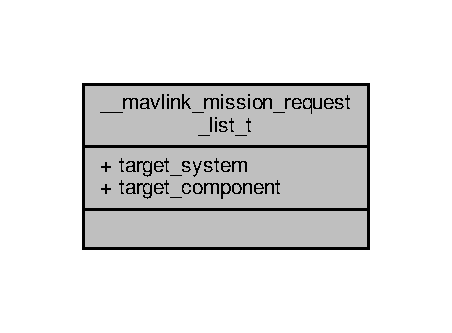
\includegraphics[width=217pt]{struct____mavlink__mission__request__list__t__coll__graph}
\end{center}
\end{figure}
\subsection*{Public Attributes}
\begin{DoxyCompactItemize}
\item 
\hypertarget{struct____mavlink__mission__request__list__t_ae8b0c8bffa1ecde59f37cdf8b65f47d4}{uint8\+\_\+t \hyperlink{struct____mavlink__mission__request__list__t_ae8b0c8bffa1ecde59f37cdf8b65f47d4}{target\+\_\+system}}\label{struct____mavlink__mission__request__list__t_ae8b0c8bffa1ecde59f37cdf8b65f47d4}

\begin{DoxyCompactList}\small\item\em System I\+D. \end{DoxyCompactList}\item 
\hypertarget{struct____mavlink__mission__request__list__t_a8214615734dcc050fdcd5ccaad31b550}{uint8\+\_\+t \hyperlink{struct____mavlink__mission__request__list__t_a8214615734dcc050fdcd5ccaad31b550}{target\+\_\+component}}\label{struct____mavlink__mission__request__list__t_a8214615734dcc050fdcd5ccaad31b550}

\begin{DoxyCompactList}\small\item\em Component I\+D. \end{DoxyCompactList}\end{DoxyCompactItemize}


The documentation for this struct was generated from the following file\+:\begin{DoxyCompactItemize}
\item 
/run/media/julien/\+Data/\+Documents/\+M\+A\+V\+R\+I\+C/\+M\+A\+V\+R\+I\+C\+\_\+\+Library/mavlink/include/common/mavlink\+\_\+msg\+\_\+mission\+\_\+request\+\_\+list.\+h\end{DoxyCompactItemize}

\hypertarget{struct____mavlink__mission__request__partial__list__t}{\section{\+\_\+\+\_\+mavlink\+\_\+mission\+\_\+request\+\_\+partial\+\_\+list\+\_\+t Struct Reference}
\label{struct____mavlink__mission__request__partial__list__t}\index{\+\_\+\+\_\+mavlink\+\_\+mission\+\_\+request\+\_\+partial\+\_\+list\+\_\+t@{\+\_\+\+\_\+mavlink\+\_\+mission\+\_\+request\+\_\+partial\+\_\+list\+\_\+t}}
}


Collaboration diagram for \+\_\+\+\_\+mavlink\+\_\+mission\+\_\+request\+\_\+partial\+\_\+list\+\_\+t\+:
\nopagebreak
\begin{figure}[H]
\begin{center}
\leavevmode
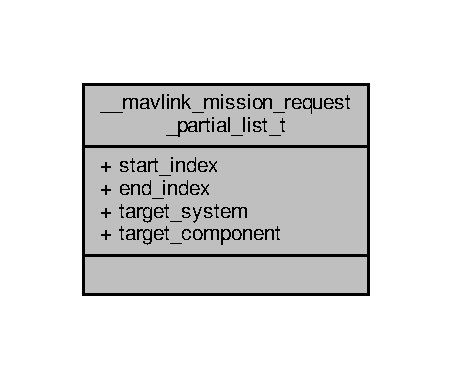
\includegraphics[width=217pt]{struct____mavlink__mission__request__partial__list__t__coll__graph}
\end{center}
\end{figure}
\subsection*{Public Attributes}
\begin{DoxyCompactItemize}
\item 
\hypertarget{struct____mavlink__mission__request__partial__list__t_aa88d56cd8a892b8416b49a6e0ec9b5cf}{int16\+\_\+t \hyperlink{struct____mavlink__mission__request__partial__list__t_aa88d56cd8a892b8416b49a6e0ec9b5cf}{start\+\_\+index}}\label{struct____mavlink__mission__request__partial__list__t_aa88d56cd8a892b8416b49a6e0ec9b5cf}

\begin{DoxyCompactList}\small\item\em Start index, 0 by default. \end{DoxyCompactList}\item 
\hypertarget{struct____mavlink__mission__request__partial__list__t_a9e484b80b2b8a0ced10f414e2d6c2636}{int16\+\_\+t \hyperlink{struct____mavlink__mission__request__partial__list__t_a9e484b80b2b8a0ced10f414e2d6c2636}{end\+\_\+index}}\label{struct____mavlink__mission__request__partial__list__t_a9e484b80b2b8a0ced10f414e2d6c2636}

\begin{DoxyCompactList}\small\item\em End index, -\/1 by default (-\/1\+: send list to end). Else a valid index of the list. \end{DoxyCompactList}\item 
\hypertarget{struct____mavlink__mission__request__partial__list__t_aa4ec7ce5b44a621b414861aa5e575cc6}{uint8\+\_\+t \hyperlink{struct____mavlink__mission__request__partial__list__t_aa4ec7ce5b44a621b414861aa5e575cc6}{target\+\_\+system}}\label{struct____mavlink__mission__request__partial__list__t_aa4ec7ce5b44a621b414861aa5e575cc6}

\begin{DoxyCompactList}\small\item\em System I\+D. \end{DoxyCompactList}\item 
\hypertarget{struct____mavlink__mission__request__partial__list__t_abc11feeb766eb42c7eadff5850284cd2}{uint8\+\_\+t \hyperlink{struct____mavlink__mission__request__partial__list__t_abc11feeb766eb42c7eadff5850284cd2}{target\+\_\+component}}\label{struct____mavlink__mission__request__partial__list__t_abc11feeb766eb42c7eadff5850284cd2}

\begin{DoxyCompactList}\small\item\em Component I\+D. \end{DoxyCompactList}\end{DoxyCompactItemize}


The documentation for this struct was generated from the following file\+:\begin{DoxyCompactItemize}
\item 
/run/media/julien/\+Data/\+Documents/\+M\+A\+V\+R\+I\+C/\+M\+A\+V\+R\+I\+C\+\_\+\+Library/mavlink/include/common/mavlink\+\_\+msg\+\_\+mission\+\_\+request\+\_\+partial\+\_\+list.\+h\end{DoxyCompactItemize}

\hypertarget{struct____mavlink__mission__request__t}{\section{\+\_\+\+\_\+mavlink\+\_\+mission\+\_\+request\+\_\+t Struct Reference}
\label{struct____mavlink__mission__request__t}\index{\+\_\+\+\_\+mavlink\+\_\+mission\+\_\+request\+\_\+t@{\+\_\+\+\_\+mavlink\+\_\+mission\+\_\+request\+\_\+t}}
}


Collaboration diagram for \+\_\+\+\_\+mavlink\+\_\+mission\+\_\+request\+\_\+t\+:
\nopagebreak
\begin{figure}[H]
\begin{center}
\leavevmode
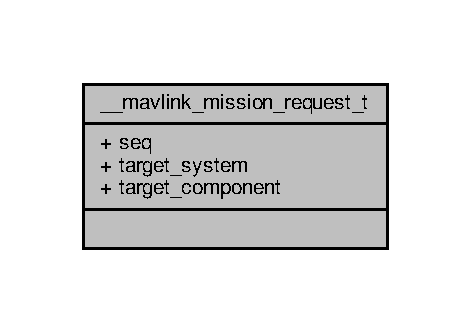
\includegraphics[width=226pt]{struct____mavlink__mission__request__t__coll__graph}
\end{center}
\end{figure}
\subsection*{Public Attributes}
\begin{DoxyCompactItemize}
\item 
\hypertarget{struct____mavlink__mission__request__t_adc8352db8e2a6dd3c5db6ec297e6d7ed}{uint16\+\_\+t \hyperlink{struct____mavlink__mission__request__t_adc8352db8e2a6dd3c5db6ec297e6d7ed}{seq}}\label{struct____mavlink__mission__request__t_adc8352db8e2a6dd3c5db6ec297e6d7ed}

\begin{DoxyCompactList}\small\item\em Sequence. \end{DoxyCompactList}\item 
\hypertarget{struct____mavlink__mission__request__t_a8e2bdf5722c43082dfccd49839f7da43}{uint8\+\_\+t \hyperlink{struct____mavlink__mission__request__t_a8e2bdf5722c43082dfccd49839f7da43}{target\+\_\+system}}\label{struct____mavlink__mission__request__t_a8e2bdf5722c43082dfccd49839f7da43}

\begin{DoxyCompactList}\small\item\em System I\+D. \end{DoxyCompactList}\item 
\hypertarget{struct____mavlink__mission__request__t_a3bef9f78c3256322231456b15601f1a6}{uint8\+\_\+t \hyperlink{struct____mavlink__mission__request__t_a3bef9f78c3256322231456b15601f1a6}{target\+\_\+component}}\label{struct____mavlink__mission__request__t_a3bef9f78c3256322231456b15601f1a6}

\begin{DoxyCompactList}\small\item\em Component I\+D. \end{DoxyCompactList}\end{DoxyCompactItemize}


The documentation for this struct was generated from the following file\+:\begin{DoxyCompactItemize}
\item 
/run/media/julien/\+Data/\+Documents/\+M\+A\+V\+R\+I\+C/\+M\+A\+V\+R\+I\+C\+\_\+\+Library/mavlink/include/common/mavlink\+\_\+msg\+\_\+mission\+\_\+request.\+h\end{DoxyCompactItemize}

\hypertarget{struct____mavlink__mission__set__current__t}{\section{\+\_\+\+\_\+mavlink\+\_\+mission\+\_\+set\+\_\+current\+\_\+t Struct Reference}
\label{struct____mavlink__mission__set__current__t}\index{\+\_\+\+\_\+mavlink\+\_\+mission\+\_\+set\+\_\+current\+\_\+t@{\+\_\+\+\_\+mavlink\+\_\+mission\+\_\+set\+\_\+current\+\_\+t}}
}


Collaboration diagram for \+\_\+\+\_\+mavlink\+\_\+mission\+\_\+set\+\_\+current\+\_\+t\+:
\nopagebreak
\begin{figure}[H]
\begin{center}
\leavevmode
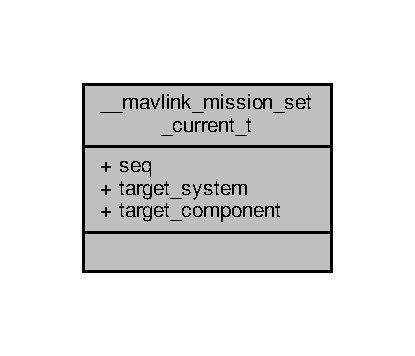
\includegraphics[width=199pt]{struct____mavlink__mission__set__current__t__coll__graph}
\end{center}
\end{figure}
\subsection*{Public Attributes}
\begin{DoxyCompactItemize}
\item 
\hypertarget{struct____mavlink__mission__set__current__t_add7d7aa3830c71875706ac4e8e5206aa}{uint16\+\_\+t \hyperlink{struct____mavlink__mission__set__current__t_add7d7aa3830c71875706ac4e8e5206aa}{seq}}\label{struct____mavlink__mission__set__current__t_add7d7aa3830c71875706ac4e8e5206aa}

\begin{DoxyCompactList}\small\item\em Sequence. \end{DoxyCompactList}\item 
\hypertarget{struct____mavlink__mission__set__current__t_aa9499477334421047ddb7b3d8e4b7794}{uint8\+\_\+t \hyperlink{struct____mavlink__mission__set__current__t_aa9499477334421047ddb7b3d8e4b7794}{target\+\_\+system}}\label{struct____mavlink__mission__set__current__t_aa9499477334421047ddb7b3d8e4b7794}

\begin{DoxyCompactList}\small\item\em System I\+D. \end{DoxyCompactList}\item 
\hypertarget{struct____mavlink__mission__set__current__t_a367ad0a39fa1fc6d06ee1aa06a9a6908}{uint8\+\_\+t \hyperlink{struct____mavlink__mission__set__current__t_a367ad0a39fa1fc6d06ee1aa06a9a6908}{target\+\_\+component}}\label{struct____mavlink__mission__set__current__t_a367ad0a39fa1fc6d06ee1aa06a9a6908}

\begin{DoxyCompactList}\small\item\em Component I\+D. \end{DoxyCompactList}\end{DoxyCompactItemize}


The documentation for this struct was generated from the following file\+:\begin{DoxyCompactItemize}
\item 
/run/media/julien/\+Data/\+Documents/\+M\+A\+V\+R\+I\+C/\+M\+A\+V\+R\+I\+C\+\_\+\+Library/mavlink/include/common/mavlink\+\_\+msg\+\_\+mission\+\_\+set\+\_\+current.\+h\end{DoxyCompactItemize}

\hypertarget{struct____mavlink__mission__write__partial__list__t}{\section{\+\_\+\+\_\+mavlink\+\_\+mission\+\_\+write\+\_\+partial\+\_\+list\+\_\+t Struct Reference}
\label{struct____mavlink__mission__write__partial__list__t}\index{\+\_\+\+\_\+mavlink\+\_\+mission\+\_\+write\+\_\+partial\+\_\+list\+\_\+t@{\+\_\+\+\_\+mavlink\+\_\+mission\+\_\+write\+\_\+partial\+\_\+list\+\_\+t}}
}


Collaboration diagram for \+\_\+\+\_\+mavlink\+\_\+mission\+\_\+write\+\_\+partial\+\_\+list\+\_\+t\+:
\nopagebreak
\begin{figure}[H]
\begin{center}
\leavevmode
\includegraphics[width=206pt]{struct____mavlink__mission__write__partial__list__t__coll__graph}
\end{center}
\end{figure}
\subsection*{Public Attributes}
\begin{DoxyCompactItemize}
\item 
\hypertarget{struct____mavlink__mission__write__partial__list__t_a7001c48ce5da88acadbcbe40a56a0e43}{int16\+\_\+t \hyperlink{struct____mavlink__mission__write__partial__list__t_a7001c48ce5da88acadbcbe40a56a0e43}{start\+\_\+index}}\label{struct____mavlink__mission__write__partial__list__t_a7001c48ce5da88acadbcbe40a56a0e43}

\begin{DoxyCompactList}\small\item\em Start index, 0 by default and smaller / equal to the largest index of the current onboard list. \end{DoxyCompactList}\item 
\hypertarget{struct____mavlink__mission__write__partial__list__t_a98971b77ca596d8a92837a0836abf489}{int16\+\_\+t \hyperlink{struct____mavlink__mission__write__partial__list__t_a98971b77ca596d8a92837a0836abf489}{end\+\_\+index}}\label{struct____mavlink__mission__write__partial__list__t_a98971b77ca596d8a92837a0836abf489}

\begin{DoxyCompactList}\small\item\em End index, equal or greater than start index. \end{DoxyCompactList}\item 
\hypertarget{struct____mavlink__mission__write__partial__list__t_aa5e77ea55d7e908035fab2d1b0beb898}{uint8\+\_\+t \hyperlink{struct____mavlink__mission__write__partial__list__t_aa5e77ea55d7e908035fab2d1b0beb898}{target\+\_\+system}}\label{struct____mavlink__mission__write__partial__list__t_aa5e77ea55d7e908035fab2d1b0beb898}

\begin{DoxyCompactList}\small\item\em System I\+D. \end{DoxyCompactList}\item 
\hypertarget{struct____mavlink__mission__write__partial__list__t_a3e0c142d5a465fe2bf22e8c728be4a58}{uint8\+\_\+t \hyperlink{struct____mavlink__mission__write__partial__list__t_a3e0c142d5a465fe2bf22e8c728be4a58}{target\+\_\+component}}\label{struct____mavlink__mission__write__partial__list__t_a3e0c142d5a465fe2bf22e8c728be4a58}

\begin{DoxyCompactList}\small\item\em Component I\+D. \end{DoxyCompactList}\end{DoxyCompactItemize}


The documentation for this struct was generated from the following file\+:\begin{DoxyCompactItemize}
\item 
/run/media/julien/\+Data/\+Documents/\+M\+A\+V\+R\+I\+C/\+M\+A\+V\+R\+I\+C\+\_\+\+Library/mavlink/include/common/mavlink\+\_\+msg\+\_\+mission\+\_\+write\+\_\+partial\+\_\+list.\+h\end{DoxyCompactItemize}

\hypertarget{struct____mavlink__named__value__float__t}{\section{\+\_\+\+\_\+mavlink\+\_\+named\+\_\+value\+\_\+float\+\_\+t Struct Reference}
\label{struct____mavlink__named__value__float__t}\index{\+\_\+\+\_\+mavlink\+\_\+named\+\_\+value\+\_\+float\+\_\+t@{\+\_\+\+\_\+mavlink\+\_\+named\+\_\+value\+\_\+float\+\_\+t}}
}


Collaboration diagram for \+\_\+\+\_\+mavlink\+\_\+named\+\_\+value\+\_\+float\+\_\+t\+:
\nopagebreak
\begin{figure}[H]
\begin{center}
\leavevmode
\includegraphics[width=204pt]{struct____mavlink__named__value__float__t__coll__graph}
\end{center}
\end{figure}
\subsection*{Public Attributes}
\begin{DoxyCompactItemize}
\item 
\hypertarget{struct____mavlink__named__value__float__t_a46e6c60e5c779ce8f3e808c485aa620f}{uint32\+\_\+t \hyperlink{struct____mavlink__named__value__float__t_a46e6c60e5c779ce8f3e808c485aa620f}{time\+\_\+boot\+\_\+ms}}\label{struct____mavlink__named__value__float__t_a46e6c60e5c779ce8f3e808c485aa620f}

\begin{DoxyCompactList}\small\item\em Timestamp (milliseconds since system boot) \end{DoxyCompactList}\item 
\hypertarget{struct____mavlink__named__value__float__t_a44c8c857d4e8732bccb9ef9ed1e2a386}{float \hyperlink{struct____mavlink__named__value__float__t_a44c8c857d4e8732bccb9ef9ed1e2a386}{value}}\label{struct____mavlink__named__value__float__t_a44c8c857d4e8732bccb9ef9ed1e2a386}

\begin{DoxyCompactList}\small\item\em Floating point value. \end{DoxyCompactList}\item 
\hypertarget{struct____mavlink__named__value__float__t_a3898dace84b76ba862dcf18a24e7e395}{char \hyperlink{struct____mavlink__named__value__float__t_a3898dace84b76ba862dcf18a24e7e395}{name} \mbox{[}10\mbox{]}}\label{struct____mavlink__named__value__float__t_a3898dace84b76ba862dcf18a24e7e395}

\begin{DoxyCompactList}\small\item\em Name of the debug variable. \end{DoxyCompactList}\end{DoxyCompactItemize}


The documentation for this struct was generated from the following file\+:\begin{DoxyCompactItemize}
\item 
/run/media/julien/\+Data/\+Documents/\+M\+A\+V\+R\+I\+C/\+M\+A\+V\+R\+I\+C\+\_\+\+Library/mavlink/include/common/mavlink\+\_\+msg\+\_\+named\+\_\+value\+\_\+float.\+h\end{DoxyCompactItemize}

\hypertarget{struct____mavlink__named__value__int__t}{\section{\+\_\+\+\_\+mavlink\+\_\+named\+\_\+value\+\_\+int\+\_\+t Struct Reference}
\label{struct____mavlink__named__value__int__t}\index{\+\_\+\+\_\+mavlink\+\_\+named\+\_\+value\+\_\+int\+\_\+t@{\+\_\+\+\_\+mavlink\+\_\+named\+\_\+value\+\_\+int\+\_\+t}}
}


Collaboration diagram for \+\_\+\+\_\+mavlink\+\_\+named\+\_\+value\+\_\+int\+\_\+t\+:
\nopagebreak
\begin{figure}[H]
\begin{center}
\leavevmode
\includegraphics[width=204pt]{struct____mavlink__named__value__int__t__coll__graph}
\end{center}
\end{figure}
\subsection*{Public Attributes}
\begin{DoxyCompactItemize}
\item 
\hypertarget{struct____mavlink__named__value__int__t_ab9e1d97f4b6a53bac6086743223c4249}{uint32\+\_\+t \hyperlink{struct____mavlink__named__value__int__t_ab9e1d97f4b6a53bac6086743223c4249}{time\+\_\+boot\+\_\+ms}}\label{struct____mavlink__named__value__int__t_ab9e1d97f4b6a53bac6086743223c4249}

\begin{DoxyCompactList}\small\item\em Timestamp (milliseconds since system boot) \end{DoxyCompactList}\item 
\hypertarget{struct____mavlink__named__value__int__t_ab6bdae0f70ba0c8bece0d206c0075fef}{int32\+\_\+t \hyperlink{struct____mavlink__named__value__int__t_ab6bdae0f70ba0c8bece0d206c0075fef}{value}}\label{struct____mavlink__named__value__int__t_ab6bdae0f70ba0c8bece0d206c0075fef}

\begin{DoxyCompactList}\small\item\em Signed integer value. \end{DoxyCompactList}\item 
\hypertarget{struct____mavlink__named__value__int__t_a3816d3a8c6130f7f9657d833ad39a202}{char \hyperlink{struct____mavlink__named__value__int__t_a3816d3a8c6130f7f9657d833ad39a202}{name} \mbox{[}10\mbox{]}}\label{struct____mavlink__named__value__int__t_a3816d3a8c6130f7f9657d833ad39a202}

\begin{DoxyCompactList}\small\item\em Name of the debug variable. \end{DoxyCompactList}\end{DoxyCompactItemize}


The documentation for this struct was generated from the following file\+:\begin{DoxyCompactItemize}
\item 
/run/media/julien/\+Data/\+Documents/\+M\+A\+V\+R\+I\+C/\+M\+A\+V\+R\+I\+C\+\_\+\+Library/mavlink/include/common/mavlink\+\_\+msg\+\_\+named\+\_\+value\+\_\+int.\+h\end{DoxyCompactItemize}

\hypertarget{struct____mavlink__nav__controller__output__t}{\section{\+\_\+\+\_\+mavlink\+\_\+nav\+\_\+controller\+\_\+output\+\_\+t Struct Reference}
\label{struct____mavlink__nav__controller__output__t}\index{\+\_\+\+\_\+mavlink\+\_\+nav\+\_\+controller\+\_\+output\+\_\+t@{\+\_\+\+\_\+mavlink\+\_\+nav\+\_\+controller\+\_\+output\+\_\+t}}
}


Collaboration diagram for \+\_\+\+\_\+mavlink\+\_\+nav\+\_\+controller\+\_\+output\+\_\+t\+:
\nopagebreak
\begin{figure}[H]
\begin{center}
\leavevmode
\includegraphics[width=207pt]{struct____mavlink__nav__controller__output__t__coll__graph}
\end{center}
\end{figure}
\subsection*{Public Attributes}
\begin{DoxyCompactItemize}
\item 
\hypertarget{struct____mavlink__nav__controller__output__t_a4d11bb9b43d937ab389aab2982ddd1c1}{float \hyperlink{struct____mavlink__nav__controller__output__t_a4d11bb9b43d937ab389aab2982ddd1c1}{nav\+\_\+roll}}\label{struct____mavlink__nav__controller__output__t_a4d11bb9b43d937ab389aab2982ddd1c1}

\begin{DoxyCompactList}\small\item\em Current desired roll in degrees. \end{DoxyCompactList}\item 
\hypertarget{struct____mavlink__nav__controller__output__t_a12445c329084694f295b51a1f5587691}{float \hyperlink{struct____mavlink__nav__controller__output__t_a12445c329084694f295b51a1f5587691}{nav\+\_\+pitch}}\label{struct____mavlink__nav__controller__output__t_a12445c329084694f295b51a1f5587691}

\begin{DoxyCompactList}\small\item\em Current desired pitch in degrees. \end{DoxyCompactList}\item 
\hypertarget{struct____mavlink__nav__controller__output__t_a40a6a20a742864361b047967ce7eb9df}{float \hyperlink{struct____mavlink__nav__controller__output__t_a40a6a20a742864361b047967ce7eb9df}{alt\+\_\+error}}\label{struct____mavlink__nav__controller__output__t_a40a6a20a742864361b047967ce7eb9df}

\begin{DoxyCompactList}\small\item\em Current altitude error in meters. \end{DoxyCompactList}\item 
\hypertarget{struct____mavlink__nav__controller__output__t_af9d8faadd55533885c61717a7a7ac407}{float \hyperlink{struct____mavlink__nav__controller__output__t_af9d8faadd55533885c61717a7a7ac407}{aspd\+\_\+error}}\label{struct____mavlink__nav__controller__output__t_af9d8faadd55533885c61717a7a7ac407}

\begin{DoxyCompactList}\small\item\em Current airspeed error in meters/second. \end{DoxyCompactList}\item 
\hypertarget{struct____mavlink__nav__controller__output__t_a98cf3736cfd6f54d24effedb10b39cd0}{float \hyperlink{struct____mavlink__nav__controller__output__t_a98cf3736cfd6f54d24effedb10b39cd0}{xtrack\+\_\+error}}\label{struct____mavlink__nav__controller__output__t_a98cf3736cfd6f54d24effedb10b39cd0}

\begin{DoxyCompactList}\small\item\em Current crosstrack error on x-\/y plane in meters. \end{DoxyCompactList}\item 
\hypertarget{struct____mavlink__nav__controller__output__t_ae18c3d9716a9ec77450d9acf03ea1f64}{int16\+\_\+t \hyperlink{struct____mavlink__nav__controller__output__t_ae18c3d9716a9ec77450d9acf03ea1f64}{nav\+\_\+bearing}}\label{struct____mavlink__nav__controller__output__t_ae18c3d9716a9ec77450d9acf03ea1f64}

\begin{DoxyCompactList}\small\item\em Current desired heading in degrees. \end{DoxyCompactList}\item 
\hypertarget{struct____mavlink__nav__controller__output__t_a4601945c2201a6dcaca7acc5154e087e}{int16\+\_\+t \hyperlink{struct____mavlink__nav__controller__output__t_a4601945c2201a6dcaca7acc5154e087e}{target\+\_\+bearing}}\label{struct____mavlink__nav__controller__output__t_a4601945c2201a6dcaca7acc5154e087e}

\begin{DoxyCompactList}\small\item\em Bearing to current M\+I\+S\+S\+I\+O\+N/target in degrees. \end{DoxyCompactList}\item 
\hypertarget{struct____mavlink__nav__controller__output__t_aa7d7186c64fdd4cf8a0ace5bd2a071f1}{uint16\+\_\+t \hyperlink{struct____mavlink__nav__controller__output__t_aa7d7186c64fdd4cf8a0ace5bd2a071f1}{wp\+\_\+dist}}\label{struct____mavlink__nav__controller__output__t_aa7d7186c64fdd4cf8a0ace5bd2a071f1}

\begin{DoxyCompactList}\small\item\em Distance to active M\+I\+S\+S\+I\+O\+N in meters. \end{DoxyCompactList}\end{DoxyCompactItemize}


The documentation for this struct was generated from the following file\+:\begin{DoxyCompactItemize}
\item 
/run/media/julien/\+Data/\+Documents/\+M\+A\+V\+R\+I\+C/\+M\+A\+V\+R\+I\+C\+\_\+\+Library/mavlink/include/common/mavlink\+\_\+msg\+\_\+nav\+\_\+controller\+\_\+output.\+h\end{DoxyCompactItemize}

\hypertarget{struct____mavlink__omnidirectional__flow__t}{\section{\+\_\+\+\_\+mavlink\+\_\+omnidirectional\+\_\+flow\+\_\+t Struct Reference}
\label{struct____mavlink__omnidirectional__flow__t}\index{\+\_\+\+\_\+mavlink\+\_\+omnidirectional\+\_\+flow\+\_\+t@{\+\_\+\+\_\+mavlink\+\_\+omnidirectional\+\_\+flow\+\_\+t}}
}


Collaboration diagram for \+\_\+\+\_\+mavlink\+\_\+omnidirectional\+\_\+flow\+\_\+t\+:
\nopagebreak
\begin{figure}[H]
\begin{center}
\leavevmode
\includegraphics[width=211pt]{struct____mavlink__omnidirectional__flow__t__coll__graph}
\end{center}
\end{figure}
\subsection*{Public Attributes}
\begin{DoxyCompactItemize}
\item 
\hypertarget{struct____mavlink__omnidirectional__flow__t_aab9c4c4e1b066f5177717903d682da31}{uint64\+\_\+t \hyperlink{struct____mavlink__omnidirectional__flow__t_aab9c4c4e1b066f5177717903d682da31}{time\+\_\+usec}}\label{struct____mavlink__omnidirectional__flow__t_aab9c4c4e1b066f5177717903d682da31}

\begin{DoxyCompactList}\small\item\em Timestamp (microseconds, synced to U\+N\+I\+X time or since system boot) \end{DoxyCompactList}\item 
\hypertarget{struct____mavlink__omnidirectional__flow__t_abe55c09994c092ad6fb028827de0a580}{float \hyperlink{struct____mavlink__omnidirectional__flow__t_abe55c09994c092ad6fb028827de0a580}{front\+\_\+distance\+\_\+m}}\label{struct____mavlink__omnidirectional__flow__t_abe55c09994c092ad6fb028827de0a580}

\begin{DoxyCompactList}\small\item\em Front distance in meters. Positive value (including zero)\+: distance known. Negative value\+: Unknown distance. \end{DoxyCompactList}\item 
\hypertarget{struct____mavlink__omnidirectional__flow__t_a6e8ae28c99c6813aa5131783a4b07434}{int16\+\_\+t \hyperlink{struct____mavlink__omnidirectional__flow__t_a6e8ae28c99c6813aa5131783a4b07434}{left} \mbox{[}10\mbox{]}}\label{struct____mavlink__omnidirectional__flow__t_a6e8ae28c99c6813aa5131783a4b07434}

\begin{DoxyCompactList}\small\item\em Flow in deci pixels (1 = 0.\+1 pixel) on left hemisphere. \end{DoxyCompactList}\item 
\hypertarget{struct____mavlink__omnidirectional__flow__t_a01a2eee9edb803f9d1864eca202c6d02}{int16\+\_\+t \hyperlink{struct____mavlink__omnidirectional__flow__t_a01a2eee9edb803f9d1864eca202c6d02}{right} \mbox{[}10\mbox{]}}\label{struct____mavlink__omnidirectional__flow__t_a01a2eee9edb803f9d1864eca202c6d02}

\begin{DoxyCompactList}\small\item\em Flow in deci pixels (1 = 0.\+1 pixel) on right hemisphere. \end{DoxyCompactList}\item 
\hypertarget{struct____mavlink__omnidirectional__flow__t_ad79dccdf4b9ab58e42b65322e678a419}{uint8\+\_\+t \hyperlink{struct____mavlink__omnidirectional__flow__t_ad79dccdf4b9ab58e42b65322e678a419}{sensor\+\_\+id}}\label{struct____mavlink__omnidirectional__flow__t_ad79dccdf4b9ab58e42b65322e678a419}

\begin{DoxyCompactList}\small\item\em Sensor I\+D. \end{DoxyCompactList}\item 
\hypertarget{struct____mavlink__omnidirectional__flow__t_a36283403fc9a72621904ccea1fc2e8e1}{uint8\+\_\+t \hyperlink{struct____mavlink__omnidirectional__flow__t_a36283403fc9a72621904ccea1fc2e8e1}{quality}}\label{struct____mavlink__omnidirectional__flow__t_a36283403fc9a72621904ccea1fc2e8e1}

\begin{DoxyCompactList}\small\item\em Optical flow quality / confidence. 0\+: bad, 255\+: maximum quality. \end{DoxyCompactList}\end{DoxyCompactItemize}


The documentation for this struct was generated from the following file\+:\begin{DoxyCompactItemize}
\item 
/run/media/julien/\+Data/\+Documents/\+M\+A\+V\+R\+I\+C/\+M\+A\+V\+R\+I\+C\+\_\+\+Library/mavlink/include/common/mavlink\+\_\+msg\+\_\+omnidirectional\+\_\+flow.\+h\end{DoxyCompactItemize}

\hypertarget{struct____mavlink__optical__flow__t}{\section{\+\_\+\+\_\+mavlink\+\_\+optical\+\_\+flow\+\_\+t Struct Reference}
\label{struct____mavlink__optical__flow__t}\index{\+\_\+\+\_\+mavlink\+\_\+optical\+\_\+flow\+\_\+t@{\+\_\+\+\_\+mavlink\+\_\+optical\+\_\+flow\+\_\+t}}
}


Collaboration diagram for \+\_\+\+\_\+mavlink\+\_\+optical\+\_\+flow\+\_\+t\+:
\nopagebreak
\begin{figure}[H]
\begin{center}
\leavevmode
\includegraphics[width=206pt]{struct____mavlink__optical__flow__t__coll__graph}
\end{center}
\end{figure}
\subsection*{Public Attributes}
\begin{DoxyCompactItemize}
\item 
\hypertarget{struct____mavlink__optical__flow__t_a01f76c236ab67155fe7770f82eb86ad6}{uint64\+\_\+t \hyperlink{struct____mavlink__optical__flow__t_a01f76c236ab67155fe7770f82eb86ad6}{time\+\_\+usec}}\label{struct____mavlink__optical__flow__t_a01f76c236ab67155fe7770f82eb86ad6}

\begin{DoxyCompactList}\small\item\em Timestamp (U\+N\+I\+X) \end{DoxyCompactList}\item 
\hypertarget{struct____mavlink__optical__flow__t_ab8fab603e276328627e4d96cc4f8b086}{float \hyperlink{struct____mavlink__optical__flow__t_ab8fab603e276328627e4d96cc4f8b086}{flow\+\_\+comp\+\_\+m\+\_\+x}}\label{struct____mavlink__optical__flow__t_ab8fab603e276328627e4d96cc4f8b086}

\begin{DoxyCompactList}\small\item\em Flow in meters in x-\/sensor direction, angular-\/speed compensated. \end{DoxyCompactList}\item 
\hypertarget{struct____mavlink__optical__flow__t_a2e39bcd7b74a5c660d1684c8e44e2cca}{float \hyperlink{struct____mavlink__optical__flow__t_a2e39bcd7b74a5c660d1684c8e44e2cca}{flow\+\_\+comp\+\_\+m\+\_\+y}}\label{struct____mavlink__optical__flow__t_a2e39bcd7b74a5c660d1684c8e44e2cca}

\begin{DoxyCompactList}\small\item\em Flow in meters in y-\/sensor direction, angular-\/speed compensated. \end{DoxyCompactList}\item 
\hypertarget{struct____mavlink__optical__flow__t_a89b39010e211494ffecc65c29fdd8c0e}{float \hyperlink{struct____mavlink__optical__flow__t_a89b39010e211494ffecc65c29fdd8c0e}{ground\+\_\+distance}}\label{struct____mavlink__optical__flow__t_a89b39010e211494ffecc65c29fdd8c0e}

\begin{DoxyCompactList}\small\item\em Ground distance in meters. Positive value\+: distance known. Negative value\+: Unknown distance. \end{DoxyCompactList}\item 
int16\+\_\+t \hyperlink{struct____mavlink__optical__flow__t_a1e1332d4eb9a84f38d32af8f32ed8c10}{flow\+\_\+x}
\begin{DoxyCompactList}\small\item\em Flow in pixels in x-\/sensor direction. \end{DoxyCompactList}\item 
int16\+\_\+t \hyperlink{struct____mavlink__optical__flow__t_aaf2884728b3ae06ec464c9cf2f8ce1c2}{flow\+\_\+y}
\begin{DoxyCompactList}\small\item\em Flow in pixels in y-\/sensor direction. \end{DoxyCompactList}\item 
\hypertarget{struct____mavlink__optical__flow__t_a196e345c474b8fc63570ebad5f947544}{uint8\+\_\+t \hyperlink{struct____mavlink__optical__flow__t_a196e345c474b8fc63570ebad5f947544}{sensor\+\_\+id}}\label{struct____mavlink__optical__flow__t_a196e345c474b8fc63570ebad5f947544}

\begin{DoxyCompactList}\small\item\em Sensor I\+D. \end{DoxyCompactList}\item 
\hypertarget{struct____mavlink__optical__flow__t_a3efb901fe9c47c88f90ddfb73d76f542}{uint8\+\_\+t \hyperlink{struct____mavlink__optical__flow__t_a3efb901fe9c47c88f90ddfb73d76f542}{quality}}\label{struct____mavlink__optical__flow__t_a3efb901fe9c47c88f90ddfb73d76f542}

\begin{DoxyCompactList}\small\item\em Optical flow quality / confidence. 0\+: bad, 255\+: maximum quality. \end{DoxyCompactList}\end{DoxyCompactItemize}


\subsection{Member Data Documentation}
\hypertarget{struct____mavlink__optical__flow__t_a1e1332d4eb9a84f38d32af8f32ed8c10}{\index{\+\_\+\+\_\+mavlink\+\_\+optical\+\_\+flow\+\_\+t@{\+\_\+\+\_\+mavlink\+\_\+optical\+\_\+flow\+\_\+t}!flow\+\_\+x@{flow\+\_\+x}}
\index{flow\+\_\+x@{flow\+\_\+x}!\+\_\+\+\_\+mavlink\+\_\+optical\+\_\+flow\+\_\+t@{\+\_\+\+\_\+mavlink\+\_\+optical\+\_\+flow\+\_\+t}}
\subsubsection[{flow\+\_\+x}]{\setlength{\rightskip}{0pt plus 5cm}int16\+\_\+t \+\_\+\+\_\+mavlink\+\_\+optical\+\_\+flow\+\_\+t\+::flow\+\_\+x}}\label{struct____mavlink__optical__flow__t_a1e1332d4eb9a84f38d32af8f32ed8c10}


Flow in pixels in x-\/sensor direction. 

Flow in pixels $\ast$ 10 in x-\/sensor direction (dezi-\/pixels) \hypertarget{struct____mavlink__optical__flow__t_aaf2884728b3ae06ec464c9cf2f8ce1c2}{\index{\+\_\+\+\_\+mavlink\+\_\+optical\+\_\+flow\+\_\+t@{\+\_\+\+\_\+mavlink\+\_\+optical\+\_\+flow\+\_\+t}!flow\+\_\+y@{flow\+\_\+y}}
\index{flow\+\_\+y@{flow\+\_\+y}!\+\_\+\+\_\+mavlink\+\_\+optical\+\_\+flow\+\_\+t@{\+\_\+\+\_\+mavlink\+\_\+optical\+\_\+flow\+\_\+t}}
\subsubsection[{flow\+\_\+y}]{\setlength{\rightskip}{0pt plus 5cm}int16\+\_\+t \+\_\+\+\_\+mavlink\+\_\+optical\+\_\+flow\+\_\+t\+::flow\+\_\+y}}\label{struct____mavlink__optical__flow__t_aaf2884728b3ae06ec464c9cf2f8ce1c2}


Flow in pixels in y-\/sensor direction. 

Flow in pixels $\ast$ 10 in y-\/sensor direction (dezi-\/pixels) 

The documentation for this struct was generated from the following file\+:\begin{DoxyCompactItemize}
\item 
/run/media/julien/\+Data/\+Documents/\+M\+A\+V\+R\+I\+C/\+M\+A\+V\+R\+I\+C\+\_\+\+Library/mavlink/include/common/mavlink\+\_\+msg\+\_\+optical\+\_\+flow.\+h\end{DoxyCompactItemize}

\hypertarget{struct____mavlink__param__request__list__t}{\section{\+\_\+\+\_\+mavlink\+\_\+param\+\_\+request\+\_\+list\+\_\+t Struct Reference}
\label{struct____mavlink__param__request__list__t}\index{\+\_\+\+\_\+mavlink\+\_\+param\+\_\+request\+\_\+list\+\_\+t@{\+\_\+\+\_\+mavlink\+\_\+param\+\_\+request\+\_\+list\+\_\+t}}
}


Collaboration diagram for \+\_\+\+\_\+mavlink\+\_\+param\+\_\+request\+\_\+list\+\_\+t\+:
\nopagebreak
\begin{figure}[H]
\begin{center}
\leavevmode
\includegraphics[width=211pt]{struct____mavlink__param__request__list__t__coll__graph}
\end{center}
\end{figure}
\subsection*{Public Attributes}
\begin{DoxyCompactItemize}
\item 
\hypertarget{struct____mavlink__param__request__list__t_aae3ba45d3ff75c3603ec6bf4eb58b244}{uint8\+\_\+t \hyperlink{struct____mavlink__param__request__list__t_aae3ba45d3ff75c3603ec6bf4eb58b244}{target\+\_\+system}}\label{struct____mavlink__param__request__list__t_aae3ba45d3ff75c3603ec6bf4eb58b244}

\begin{DoxyCompactList}\small\item\em System I\+D. \end{DoxyCompactList}\item 
\hypertarget{struct____mavlink__param__request__list__t_adf6602f61af11ec222fdabd850abdf2d}{uint8\+\_\+t \hyperlink{struct____mavlink__param__request__list__t_adf6602f61af11ec222fdabd850abdf2d}{target\+\_\+component}}\label{struct____mavlink__param__request__list__t_adf6602f61af11ec222fdabd850abdf2d}

\begin{DoxyCompactList}\small\item\em Component I\+D. \end{DoxyCompactList}\end{DoxyCompactItemize}


The documentation for this struct was generated from the following file\+:\begin{DoxyCompactItemize}
\item 
/run/media/julien/\+Data/\+Documents/\+M\+A\+V\+R\+I\+C/\+M\+A\+V\+R\+I\+C\+\_\+\+Library/mavlink/include/common/mavlink\+\_\+msg\+\_\+param\+\_\+request\+\_\+list.\+h\end{DoxyCompactItemize}

\hypertarget{struct____mavlink__param__request__read__t}{\section{\+\_\+\+\_\+mavlink\+\_\+param\+\_\+request\+\_\+read\+\_\+t Struct Reference}
\label{struct____mavlink__param__request__read__t}\index{\+\_\+\+\_\+mavlink\+\_\+param\+\_\+request\+\_\+read\+\_\+t@{\+\_\+\+\_\+mavlink\+\_\+param\+\_\+request\+\_\+read\+\_\+t}}
}


Collaboration diagram for \+\_\+\+\_\+mavlink\+\_\+param\+\_\+request\+\_\+read\+\_\+t\+:
\nopagebreak
\begin{figure}[H]
\begin{center}
\leavevmode
\includegraphics[width=211pt]{struct____mavlink__param__request__read__t__coll__graph}
\end{center}
\end{figure}
\subsection*{Public Attributes}
\begin{DoxyCompactItemize}
\item 
\hypertarget{struct____mavlink__param__request__read__t_aef0bfa3c1d8457e0b417fa87b31f3c22}{int16\+\_\+t \hyperlink{struct____mavlink__param__request__read__t_aef0bfa3c1d8457e0b417fa87b31f3c22}{param\+\_\+index}}\label{struct____mavlink__param__request__read__t_aef0bfa3c1d8457e0b417fa87b31f3c22}

\begin{DoxyCompactList}\small\item\em Parameter index. Send -\/1 to use the param I\+D field as identifier (else the param id will be ignored) \end{DoxyCompactList}\item 
\hypertarget{struct____mavlink__param__request__read__t_adc4407f944beba256a385768ea61e588}{uint8\+\_\+t \hyperlink{struct____mavlink__param__request__read__t_adc4407f944beba256a385768ea61e588}{target\+\_\+system}}\label{struct____mavlink__param__request__read__t_adc4407f944beba256a385768ea61e588}

\begin{DoxyCompactList}\small\item\em System I\+D. \end{DoxyCompactList}\item 
\hypertarget{struct____mavlink__param__request__read__t_aa865f64059877480b11a2f476d1a8ca4}{uint8\+\_\+t \hyperlink{struct____mavlink__param__request__read__t_aa865f64059877480b11a2f476d1a8ca4}{target\+\_\+component}}\label{struct____mavlink__param__request__read__t_aa865f64059877480b11a2f476d1a8ca4}

\begin{DoxyCompactList}\small\item\em Component I\+D. \end{DoxyCompactList}\item 
\hypertarget{struct____mavlink__param__request__read__t_a4b68020afd08464492f33950e77d9219}{char \hyperlink{struct____mavlink__param__request__read__t_a4b68020afd08464492f33950e77d9219}{param\+\_\+id} \mbox{[}16\mbox{]}}\label{struct____mavlink__param__request__read__t_a4b68020afd08464492f33950e77d9219}

\begin{DoxyCompactList}\small\item\em Onboard parameter id, terminated by N\+U\+L\+L if the length is less than 16 human-\/readable chars and W\+I\+T\+H\+O\+U\+T null termination (N\+U\+L\+L) byte if the length is exactly 16 chars -\/ applications have to provide 16+1 bytes storage if the I\+D is stored as string. \end{DoxyCompactList}\end{DoxyCompactItemize}


The documentation for this struct was generated from the following file\+:\begin{DoxyCompactItemize}
\item 
/run/media/julien/\+Data/\+Documents/\+M\+A\+V\+R\+I\+C/\+M\+A\+V\+R\+I\+C\+\_\+\+Library/mavlink/include/common/mavlink\+\_\+msg\+\_\+param\+\_\+request\+\_\+read.\+h\end{DoxyCompactItemize}

\hypertarget{struct____mavlink__param__set__t}{\section{\+\_\+\+\_\+mavlink\+\_\+param\+\_\+set\+\_\+t Struct Reference}
\label{struct____mavlink__param__set__t}\index{\+\_\+\+\_\+mavlink\+\_\+param\+\_\+set\+\_\+t@{\+\_\+\+\_\+mavlink\+\_\+param\+\_\+set\+\_\+t}}
}


Collaboration diagram for \+\_\+\+\_\+mavlink\+\_\+param\+\_\+set\+\_\+t\+:
\nopagebreak
\begin{figure}[H]
\begin{center}
\leavevmode
\includegraphics[width=200pt]{struct____mavlink__param__set__t__coll__graph}
\end{center}
\end{figure}
\subsection*{Public Attributes}
\begin{DoxyCompactItemize}
\item 
\hypertarget{struct____mavlink__param__set__t_a210adccaf668137e5f083c825804276e}{float \hyperlink{struct____mavlink__param__set__t_a210adccaf668137e5f083c825804276e}{param\+\_\+value}}\label{struct____mavlink__param__set__t_a210adccaf668137e5f083c825804276e}

\begin{DoxyCompactList}\small\item\em Onboard parameter value. \end{DoxyCompactList}\item 
\hypertarget{struct____mavlink__param__set__t_a501eee1b0a93fa7affad440d51bbab90}{uint8\+\_\+t \hyperlink{struct____mavlink__param__set__t_a501eee1b0a93fa7affad440d51bbab90}{target\+\_\+system}}\label{struct____mavlink__param__set__t_a501eee1b0a93fa7affad440d51bbab90}

\begin{DoxyCompactList}\small\item\em System I\+D. \end{DoxyCompactList}\item 
\hypertarget{struct____mavlink__param__set__t_ad1526f09aefc29226f2362a2a0963237}{uint8\+\_\+t \hyperlink{struct____mavlink__param__set__t_ad1526f09aefc29226f2362a2a0963237}{target\+\_\+component}}\label{struct____mavlink__param__set__t_ad1526f09aefc29226f2362a2a0963237}

\begin{DoxyCompactList}\small\item\em Component I\+D. \end{DoxyCompactList}\item 
\hypertarget{struct____mavlink__param__set__t_acd97fee9abc903096a392cb9b4b78369}{char \hyperlink{struct____mavlink__param__set__t_acd97fee9abc903096a392cb9b4b78369}{param\+\_\+id} \mbox{[}16\mbox{]}}\label{struct____mavlink__param__set__t_acd97fee9abc903096a392cb9b4b78369}

\begin{DoxyCompactList}\small\item\em Onboard parameter id, terminated by N\+U\+L\+L if the length is less than 16 human-\/readable chars and W\+I\+T\+H\+O\+U\+T null termination (N\+U\+L\+L) byte if the length is exactly 16 chars -\/ applications have to provide 16+1 bytes storage if the I\+D is stored as string. \end{DoxyCompactList}\item 
\hypertarget{struct____mavlink__param__set__t_a4eb99cce0725481254d653290a06de6f}{uint8\+\_\+t \hyperlink{struct____mavlink__param__set__t_a4eb99cce0725481254d653290a06de6f}{param\+\_\+type}}\label{struct____mavlink__param__set__t_a4eb99cce0725481254d653290a06de6f}

\begin{DoxyCompactList}\small\item\em Onboard parameter type\+: see the M\+A\+V\+\_\+\+P\+A\+R\+A\+M\+\_\+\+T\+Y\+P\+E enum for supported data types. \end{DoxyCompactList}\end{DoxyCompactItemize}


The documentation for this struct was generated from the following file\+:\begin{DoxyCompactItemize}
\item 
/run/media/julien/\+Data/\+Documents/\+M\+A\+V\+R\+I\+C/\+M\+A\+V\+R\+I\+C\+\_\+\+Library/mavlink/include/common/mavlink\+\_\+msg\+\_\+param\+\_\+set.\+h\end{DoxyCompactItemize}

\hypertarget{struct____mavlink__param__value__t}{\section{\+\_\+\+\_\+mavlink\+\_\+param\+\_\+value\+\_\+t Struct Reference}
\label{struct____mavlink__param__value__t}\index{\+\_\+\+\_\+mavlink\+\_\+param\+\_\+value\+\_\+t@{\+\_\+\+\_\+mavlink\+\_\+param\+\_\+value\+\_\+t}}
}


Collaboration diagram for \+\_\+\+\_\+mavlink\+\_\+param\+\_\+value\+\_\+t\+:
\nopagebreak
\begin{figure}[H]
\begin{center}
\leavevmode
\includegraphics[width=210pt]{struct____mavlink__param__value__t__coll__graph}
\end{center}
\end{figure}
\subsection*{Public Attributes}
\begin{DoxyCompactItemize}
\item 
\hypertarget{struct____mavlink__param__value__t_acd7d6401383f92dac17a95946b501a50}{float \hyperlink{struct____mavlink__param__value__t_acd7d6401383f92dac17a95946b501a50}{param\+\_\+value}}\label{struct____mavlink__param__value__t_acd7d6401383f92dac17a95946b501a50}

\begin{DoxyCompactList}\small\item\em Onboard parameter value. \end{DoxyCompactList}\item 
\hypertarget{struct____mavlink__param__value__t_ab53bec8370ac590fc761b9a9de49f6b6}{uint16\+\_\+t \hyperlink{struct____mavlink__param__value__t_ab53bec8370ac590fc761b9a9de49f6b6}{param\+\_\+count}}\label{struct____mavlink__param__value__t_ab53bec8370ac590fc761b9a9de49f6b6}

\begin{DoxyCompactList}\small\item\em Total number of onboard parameters. \end{DoxyCompactList}\item 
\hypertarget{struct____mavlink__param__value__t_a213d71adbd95b241f962dd1d375c3a5a}{uint16\+\_\+t \hyperlink{struct____mavlink__param__value__t_a213d71adbd95b241f962dd1d375c3a5a}{param\+\_\+index}}\label{struct____mavlink__param__value__t_a213d71adbd95b241f962dd1d375c3a5a}

\begin{DoxyCompactList}\small\item\em Index of this onboard parameter. \end{DoxyCompactList}\item 
\hypertarget{struct____mavlink__param__value__t_a601c9a44cc42ba2ab13d0778aa4b8d96}{char \hyperlink{struct____mavlink__param__value__t_a601c9a44cc42ba2ab13d0778aa4b8d96}{param\+\_\+id} \mbox{[}16\mbox{]}}\label{struct____mavlink__param__value__t_a601c9a44cc42ba2ab13d0778aa4b8d96}

\begin{DoxyCompactList}\small\item\em Onboard parameter id, terminated by N\+U\+L\+L if the length is less than 16 human-\/readable chars and W\+I\+T\+H\+O\+U\+T null termination (N\+U\+L\+L) byte if the length is exactly 16 chars -\/ applications have to provide 16+1 bytes storage if the I\+D is stored as string. \end{DoxyCompactList}\item 
\hypertarget{struct____mavlink__param__value__t_a825cfefbe7cfd71991186c4ffc897447}{uint8\+\_\+t \hyperlink{struct____mavlink__param__value__t_a825cfefbe7cfd71991186c4ffc897447}{param\+\_\+type}}\label{struct____mavlink__param__value__t_a825cfefbe7cfd71991186c4ffc897447}

\begin{DoxyCompactList}\small\item\em Onboard parameter type\+: see the M\+A\+V\+\_\+\+P\+A\+R\+A\+M\+\_\+\+T\+Y\+P\+E enum for supported data types. \end{DoxyCompactList}\end{DoxyCompactItemize}


The documentation for this struct was generated from the following file\+:\begin{DoxyCompactItemize}
\item 
/run/media/julien/\+Data/\+Documents/\+M\+A\+V\+R\+I\+C/\+M\+A\+V\+R\+I\+C\+\_\+\+Library/mavlink/include/common/mavlink\+\_\+msg\+\_\+param\+\_\+value.\+h\end{DoxyCompactItemize}

\hypertarget{struct____mavlink__ping__t}{\section{\+\_\+\+\_\+mavlink\+\_\+ping\+\_\+t Struct Reference}
\label{struct____mavlink__ping__t}\index{\+\_\+\+\_\+mavlink\+\_\+ping\+\_\+t@{\+\_\+\+\_\+mavlink\+\_\+ping\+\_\+t}}
}


Collaboration diagram for \+\_\+\+\_\+mavlink\+\_\+ping\+\_\+t\+:
\nopagebreak
\begin{figure}[H]
\begin{center}
\leavevmode
\includegraphics[width=184pt]{struct____mavlink__ping__t__coll__graph}
\end{center}
\end{figure}
\subsection*{Public Attributes}
\begin{DoxyCompactItemize}
\item 
\hypertarget{struct____mavlink__ping__t_a78bf2339554a175c2b5423fee61cf619}{uint64\+\_\+t \hyperlink{struct____mavlink__ping__t_a78bf2339554a175c2b5423fee61cf619}{time\+\_\+usec}}\label{struct____mavlink__ping__t_a78bf2339554a175c2b5423fee61cf619}

\begin{DoxyCompactList}\small\item\em Unix timestamp in microseconds. \end{DoxyCompactList}\item 
\hypertarget{struct____mavlink__ping__t_a753c4aa80232a414c05065646175bf46}{uint32\+\_\+t \hyperlink{struct____mavlink__ping__t_a753c4aa80232a414c05065646175bf46}{seq}}\label{struct____mavlink__ping__t_a753c4aa80232a414c05065646175bf46}

\begin{DoxyCompactList}\small\item\em P\+I\+N\+G sequence. \end{DoxyCompactList}\item 
\hypertarget{struct____mavlink__ping__t_a349dd7a0a95dc0a9faef1a498172efe3}{uint8\+\_\+t \hyperlink{struct____mavlink__ping__t_a349dd7a0a95dc0a9faef1a498172efe3}{target\+\_\+system}}\label{struct____mavlink__ping__t_a349dd7a0a95dc0a9faef1a498172efe3}

\begin{DoxyCompactList}\small\item\em 0\+: request ping from all receiving systems, if greater than 0\+: message is a ping response and number is the system id of the requesting system \end{DoxyCompactList}\item 
\hypertarget{struct____mavlink__ping__t_aea8c79743c35ac8e9d3d3362e2723f17}{uint8\+\_\+t \hyperlink{struct____mavlink__ping__t_aea8c79743c35ac8e9d3d3362e2723f17}{target\+\_\+component}}\label{struct____mavlink__ping__t_aea8c79743c35ac8e9d3d3362e2723f17}

\begin{DoxyCompactList}\small\item\em 0\+: request ping from all receiving components, if greater than 0\+: message is a ping response and number is the system id of the requesting system \end{DoxyCompactList}\end{DoxyCompactItemize}


The documentation for this struct was generated from the following file\+:\begin{DoxyCompactItemize}
\item 
/run/media/julien/\+Data/\+Documents/\+M\+A\+V\+R\+I\+C/\+M\+A\+V\+R\+I\+C\+\_\+\+Library/mavlink/include/common/mavlink\+\_\+msg\+\_\+ping.\+h\end{DoxyCompactItemize}

\hypertarget{struct____mavlink__radar__raw__data__t}{\section{\+\_\+\+\_\+mavlink\+\_\+radar\+\_\+raw\+\_\+data\+\_\+t Struct Reference}
\label{struct____mavlink__radar__raw__data__t}\index{\+\_\+\+\_\+mavlink\+\_\+radar\+\_\+raw\+\_\+data\+\_\+t@{\+\_\+\+\_\+mavlink\+\_\+radar\+\_\+raw\+\_\+data\+\_\+t}}
}


Collaboration diagram for \+\_\+\+\_\+mavlink\+\_\+radar\+\_\+raw\+\_\+data\+\_\+t\+:
\nopagebreak
\begin{figure}[H]
\begin{center}
\leavevmode
\includegraphics[width=189pt]{struct____mavlink__radar__raw__data__t__coll__graph}
\end{center}
\end{figure}
\subsection*{Public Attributes}
\begin{DoxyCompactItemize}
\item 
\hypertarget{struct____mavlink__radar__raw__data__t_a9aa87b975234ce4ccedfb2ce4a79fc31}{uint32\+\_\+t \hyperlink{struct____mavlink__radar__raw__data__t_a9aa87b975234ce4ccedfb2ce4a79fc31}{time\+\_\+boot\+\_\+ms}}\label{struct____mavlink__radar__raw__data__t_a9aa87b975234ce4ccedfb2ce4a79fc31}

\begin{DoxyCompactList}\small\item\em Timestamp (milliseconds since system boot) \end{DoxyCompactList}\item 
\hypertarget{struct____mavlink__radar__raw__data__t_aae72775aa3276681f14c48c062716f8a}{int16\+\_\+t \hyperlink{struct____mavlink__radar__raw__data__t_aae72775aa3276681f14c48c062716f8a}{values} \mbox{[}64\mbox{]}}\label{struct____mavlink__radar__raw__data__t_aae72775aa3276681f14c48c062716f8a}

\begin{DoxyCompactList}\small\item\em raw sample values \end{DoxyCompactList}\item 
\hypertarget{struct____mavlink__radar__raw__data__t_a678694a34c45b74bef35a6bb9880d14a}{uint8\+\_\+t \hyperlink{struct____mavlink__radar__raw__data__t_a678694a34c45b74bef35a6bb9880d14a}{sensor\+\_\+id}}\label{struct____mavlink__radar__raw__data__t_a678694a34c45b74bef35a6bb9880d14a}

\begin{DoxyCompactList}\small\item\em Sensor I\+D. \end{DoxyCompactList}\end{DoxyCompactItemize}


The documentation for this struct was generated from the following file\+:\begin{DoxyCompactItemize}
\item 
/run/media/julien/\+Data/\+Documents/\+M\+A\+V\+R\+I\+C/\+M\+A\+V\+R\+I\+C\+\_\+\+Library/mavlink/include/maveric/mavlink\+\_\+msg\+\_\+radar\+\_\+raw\+\_\+data.\+h\end{DoxyCompactItemize}

\hypertarget{struct____mavlink__radar__tracked__target__t}{\section{\+\_\+\+\_\+mavlink\+\_\+radar\+\_\+tracked\+\_\+target\+\_\+t Struct Reference}
\label{struct____mavlink__radar__tracked__target__t}\index{\+\_\+\+\_\+mavlink\+\_\+radar\+\_\+tracked\+\_\+target\+\_\+t@{\+\_\+\+\_\+mavlink\+\_\+radar\+\_\+tracked\+\_\+target\+\_\+t}}
}


Collaboration diagram for \+\_\+\+\_\+mavlink\+\_\+radar\+\_\+tracked\+\_\+target\+\_\+t\+:
\nopagebreak
\begin{figure}[H]
\begin{center}
\leavevmode
\includegraphics[width=205pt]{struct____mavlink__radar__tracked__target__t__coll__graph}
\end{center}
\end{figure}
\subsection*{Public Attributes}
\begin{DoxyCompactItemize}
\item 
\hypertarget{struct____mavlink__radar__tracked__target__t_a4fbde1e8d43302af33eed4f4d3e5b8cc}{uint32\+\_\+t \hyperlink{struct____mavlink__radar__tracked__target__t_a4fbde1e8d43302af33eed4f4d3e5b8cc}{time\+\_\+boot\+\_\+ms}}\label{struct____mavlink__radar__tracked__target__t_a4fbde1e8d43302af33eed4f4d3e5b8cc}

\begin{DoxyCompactList}\small\item\em Timestamp (milliseconds since system boot) \end{DoxyCompactList}\item 
\hypertarget{struct____mavlink__radar__tracked__target__t_ac2b261f4add35857d88410dd77189327}{float \hyperlink{struct____mavlink__radar__tracked__target__t_ac2b261f4add35857d88410dd77189327}{velocity}}\label{struct____mavlink__radar__tracked__target__t_ac2b261f4add35857d88410dd77189327}

\begin{DoxyCompactList}\small\item\em Velocity estimate. \end{DoxyCompactList}\item 
\hypertarget{struct____mavlink__radar__tracked__target__t_a070dd549bec561a35d6b125d7d775a9b}{float \hyperlink{struct____mavlink__radar__tracked__target__t_a070dd549bec561a35d6b125d7d775a9b}{amplitude}}\label{struct____mavlink__radar__tracked__target__t_a070dd549bec561a35d6b125d7d775a9b}

\begin{DoxyCompactList}\small\item\em Amplitude (signal strength) \end{DoxyCompactList}\item 
\hypertarget{struct____mavlink__radar__tracked__target__t_a25e85cda1fbd9c07f57a40c0a7d2a127}{float \hyperlink{struct____mavlink__radar__tracked__target__t_a25e85cda1fbd9c07f57a40c0a7d2a127}{distance}}\label{struct____mavlink__radar__tracked__target__t_a25e85cda1fbd9c07f57a40c0a7d2a127}

\begin{DoxyCompactList}\small\item\em Distance estimate. \end{DoxyCompactList}\item 
\hypertarget{struct____mavlink__radar__tracked__target__t_a0194c590ef31f1fd6682df4e8d1c3b20}{float \hyperlink{struct____mavlink__radar__tracked__target__t_a0194c590ef31f1fd6682df4e8d1c3b20}{azimuth}}\label{struct____mavlink__radar__tracked__target__t_a0194c590ef31f1fd6682df4e8d1c3b20}

\begin{DoxyCompactList}\small\item\em Azimuth. \end{DoxyCompactList}\item 
\hypertarget{struct____mavlink__radar__tracked__target__t_a85946ead59d1438a0ee0b9be417c162b}{float \hyperlink{struct____mavlink__radar__tracked__target__t_a85946ead59d1438a0ee0b9be417c162b}{elevation}}\label{struct____mavlink__radar__tracked__target__t_a85946ead59d1438a0ee0b9be417c162b}

\begin{DoxyCompactList}\small\item\em Elevation. \end{DoxyCompactList}\item 
\hypertarget{struct____mavlink__radar__tracked__target__t_a5691e22005ab2fbc665142fba1f3fab5}{float \hyperlink{struct____mavlink__radar__tracked__target__t_a5691e22005ab2fbc665142fba1f3fab5}{uncertainty}}\label{struct____mavlink__radar__tracked__target__t_a5691e22005ab2fbc665142fba1f3fab5}

\begin{DoxyCompactList}\small\item\em Uncertainty. \end{DoxyCompactList}\item 
\hypertarget{struct____mavlink__radar__tracked__target__t_ab908ac1fc8cc3e4037ec1d41f9067b1d}{uint8\+\_\+t \hyperlink{struct____mavlink__radar__tracked__target__t_ab908ac1fc8cc3e4037ec1d41f9067b1d}{sensor\+\_\+id}}\label{struct____mavlink__radar__tracked__target__t_ab908ac1fc8cc3e4037ec1d41f9067b1d}

\begin{DoxyCompactList}\small\item\em Sensor I\+D. \end{DoxyCompactList}\item 
\hypertarget{struct____mavlink__radar__tracked__target__t_a2bcb68fbc83b7b8f3aa5565528b83d2c}{uint8\+\_\+t \hyperlink{struct____mavlink__radar__tracked__target__t_a2bcb68fbc83b7b8f3aa5565528b83d2c}{target\+\_\+id}}\label{struct____mavlink__radar__tracked__target__t_a2bcb68fbc83b7b8f3aa5565528b83d2c}

\begin{DoxyCompactList}\small\item\em Temporary enumeration of target. \end{DoxyCompactList}\end{DoxyCompactItemize}


The documentation for this struct was generated from the following file\+:\begin{DoxyCompactItemize}
\item 
/run/media/julien/\+Data/\+Documents/\+M\+A\+V\+R\+I\+C/\+M\+A\+V\+R\+I\+C\+\_\+\+Library/mavlink/include/maveric/mavlink\+\_\+msg\+\_\+radar\+\_\+tracked\+\_\+target.\+h\end{DoxyCompactItemize}

\hypertarget{struct____mavlink__radar__velocity__hist__t}{\section{\+\_\+\+\_\+mavlink\+\_\+radar\+\_\+velocity\+\_\+hist\+\_\+t Struct Reference}
\label{struct____mavlink__radar__velocity__hist__t}\index{\+\_\+\+\_\+mavlink\+\_\+radar\+\_\+velocity\+\_\+hist\+\_\+t@{\+\_\+\+\_\+mavlink\+\_\+radar\+\_\+velocity\+\_\+hist\+\_\+t}}
}


Collaboration diagram for \+\_\+\+\_\+mavlink\+\_\+radar\+\_\+velocity\+\_\+hist\+\_\+t\+:
\nopagebreak
\begin{figure}[H]
\begin{center}
\leavevmode
\includegraphics[width=207pt]{struct____mavlink__radar__velocity__hist__t__coll__graph}
\end{center}
\end{figure}
\subsection*{Public Attributes}
\begin{DoxyCompactItemize}
\item 
\hypertarget{struct____mavlink__radar__velocity__hist__t_aa4dc91375e83f590224394343a6ecdcb}{uint32\+\_\+t \hyperlink{struct____mavlink__radar__velocity__hist__t_aa4dc91375e83f590224394343a6ecdcb}{time\+\_\+boot\+\_\+ms}}\label{struct____mavlink__radar__velocity__hist__t_aa4dc91375e83f590224394343a6ecdcb}

\begin{DoxyCompactList}\small\item\em Timestamp (milliseconds since system boot) \end{DoxyCompactList}\item 
\hypertarget{struct____mavlink__radar__velocity__hist__t_a4cc3b80cee5a14b5977ff661e5d41d22}{uint8\+\_\+t \hyperlink{struct____mavlink__radar__velocity__hist__t_a4cc3b80cee5a14b5977ff661e5d41d22}{sensor\+\_\+id}}\label{struct____mavlink__radar__velocity__hist__t_a4cc3b80cee5a14b5977ff661e5d41d22}

\begin{DoxyCompactList}\small\item\em Sensor I\+D. \end{DoxyCompactList}\item 
\hypertarget{struct____mavlink__radar__velocity__hist__t_a70e557375dac2acee52e20388c9d4a8f}{uint8\+\_\+t \hyperlink{struct____mavlink__radar__velocity__hist__t_a70e557375dac2acee52e20388c9d4a8f}{velocity} \mbox{[}64\mbox{]}}\label{struct____mavlink__radar__velocity__hist__t_a70e557375dac2acee52e20388c9d4a8f}

\begin{DoxyCompactList}\small\item\em Velocity field. \end{DoxyCompactList}\end{DoxyCompactItemize}


The documentation for this struct was generated from the following file\+:\begin{DoxyCompactItemize}
\item 
/run/media/julien/\+Data/\+Documents/\+M\+A\+V\+R\+I\+C/\+M\+A\+V\+R\+I\+C\+\_\+\+Library/mavlink/include/maveric/mavlink\+\_\+msg\+\_\+radar\+\_\+velocity\+\_\+hist.\+h\end{DoxyCompactItemize}

\hypertarget{struct____mavlink__radio__status__t}{\section{\+\_\+\+\_\+mavlink\+\_\+radio\+\_\+status\+\_\+t Struct Reference}
\label{struct____mavlink__radio__status__t}\index{\+\_\+\+\_\+mavlink\+\_\+radio\+\_\+status\+\_\+t@{\+\_\+\+\_\+mavlink\+\_\+radio\+\_\+status\+\_\+t}}
}


Collaboration diagram for \+\_\+\+\_\+mavlink\+\_\+radio\+\_\+status\+\_\+t\+:
\nopagebreak
\begin{figure}[H]
\begin{center}
\leavevmode
\includegraphics[width=208pt]{struct____mavlink__radio__status__t__coll__graph}
\end{center}
\end{figure}
\subsection*{Public Attributes}
\begin{DoxyCompactItemize}
\item 
\hypertarget{struct____mavlink__radio__status__t_a8685a765f489e5c207d15d2d327744d8}{uint16\+\_\+t \hyperlink{struct____mavlink__radio__status__t_a8685a765f489e5c207d15d2d327744d8}{rxerrors}}\label{struct____mavlink__radio__status__t_a8685a765f489e5c207d15d2d327744d8}

\begin{DoxyCompactList}\small\item\em receive errors \end{DoxyCompactList}\item 
\hypertarget{struct____mavlink__radio__status__t_a7963729a484bb7268e6723a0076020c1}{uint16\+\_\+t \hyperlink{struct____mavlink__radio__status__t_a7963729a484bb7268e6723a0076020c1}{fixed}}\label{struct____mavlink__radio__status__t_a7963729a484bb7268e6723a0076020c1}

\begin{DoxyCompactList}\small\item\em count of error corrected packets \end{DoxyCompactList}\item 
\hypertarget{struct____mavlink__radio__status__t_a3094eceaedbb2f0d7e501a0ae29b1153}{uint8\+\_\+t \hyperlink{struct____mavlink__radio__status__t_a3094eceaedbb2f0d7e501a0ae29b1153}{rssi}}\label{struct____mavlink__radio__status__t_a3094eceaedbb2f0d7e501a0ae29b1153}

\begin{DoxyCompactList}\small\item\em local signal strength \end{DoxyCompactList}\item 
\hypertarget{struct____mavlink__radio__status__t_a300013070ad97c6c8cb6390c4d12e9d6}{uint8\+\_\+t \hyperlink{struct____mavlink__radio__status__t_a300013070ad97c6c8cb6390c4d12e9d6}{remrssi}}\label{struct____mavlink__radio__status__t_a300013070ad97c6c8cb6390c4d12e9d6}

\begin{DoxyCompactList}\small\item\em remote signal strength \end{DoxyCompactList}\item 
\hypertarget{struct____mavlink__radio__status__t_a8f9a9b8d333b127422cb8d5b8b2b1928}{uint8\+\_\+t \hyperlink{struct____mavlink__radio__status__t_a8f9a9b8d333b127422cb8d5b8b2b1928}{txbuf}}\label{struct____mavlink__radio__status__t_a8f9a9b8d333b127422cb8d5b8b2b1928}

\begin{DoxyCompactList}\small\item\em how full the tx buffer is as a percentage \end{DoxyCompactList}\item 
\hypertarget{struct____mavlink__radio__status__t_adfe004fd757a44f0b4cdb6c15c9a1bde}{uint8\+\_\+t \hyperlink{struct____mavlink__radio__status__t_adfe004fd757a44f0b4cdb6c15c9a1bde}{noise}}\label{struct____mavlink__radio__status__t_adfe004fd757a44f0b4cdb6c15c9a1bde}

\begin{DoxyCompactList}\small\item\em background noise level \end{DoxyCompactList}\item 
\hypertarget{struct____mavlink__radio__status__t_a8c72fbe2cc42a71933ed93aa3064f2f4}{uint8\+\_\+t \hyperlink{struct____mavlink__radio__status__t_a8c72fbe2cc42a71933ed93aa3064f2f4}{remnoise}}\label{struct____mavlink__radio__status__t_a8c72fbe2cc42a71933ed93aa3064f2f4}

\begin{DoxyCompactList}\small\item\em remote background noise level \end{DoxyCompactList}\end{DoxyCompactItemize}


The documentation for this struct was generated from the following file\+:\begin{DoxyCompactItemize}
\item 
/run/media/julien/\+Data/\+Documents/\+M\+A\+V\+R\+I\+C/\+M\+A\+V\+R\+I\+C\+\_\+\+Library/mavlink/include/maveric/mavlink\+\_\+msg\+\_\+radio\+\_\+status.\+h\end{DoxyCompactItemize}

\hypertarget{struct____mavlink__raw__data__stream__descriptor__t}{\section{\+\_\+\+\_\+mavlink\+\_\+raw\+\_\+data\+\_\+stream\+\_\+descriptor\+\_\+t Struct Reference}
\label{struct____mavlink__raw__data__stream__descriptor__t}\index{\+\_\+\+\_\+mavlink\+\_\+raw\+\_\+data\+\_\+stream\+\_\+descriptor\+\_\+t@{\+\_\+\+\_\+mavlink\+\_\+raw\+\_\+data\+\_\+stream\+\_\+descriptor\+\_\+t}}
}


Collaboration diagram for \+\_\+\+\_\+mavlink\+\_\+raw\+\_\+data\+\_\+stream\+\_\+descriptor\+\_\+t\+:
\nopagebreak
\begin{figure}[H]
\begin{center}
\leavevmode
\includegraphics[width=188pt]{struct____mavlink__raw__data__stream__descriptor__t__coll__graph}
\end{center}
\end{figure}
\subsection*{Public Attributes}
\begin{DoxyCompactItemize}
\item 
\hypertarget{struct____mavlink__raw__data__stream__descriptor__t_ab6d6df3b40a653423ae90bc51644fcb6}{uint32\+\_\+t \hyperlink{struct____mavlink__raw__data__stream__descriptor__t_ab6d6df3b40a653423ae90bc51644fcb6}{time\+\_\+boot\+\_\+ms}}\label{struct____mavlink__raw__data__stream__descriptor__t_ab6d6df3b40a653423ae90bc51644fcb6}

\begin{DoxyCompactList}\small\item\em Timestamp (milliseconds since system boot) \end{DoxyCompactList}\item 
\hypertarget{struct____mavlink__raw__data__stream__descriptor__t_afb4df5a715652709786d43aa319774f7}{uint32\+\_\+t \hyperlink{struct____mavlink__raw__data__stream__descriptor__t_afb4df5a715652709786d43aa319774f7}{sample\+\_\+count}}\label{struct____mavlink__raw__data__stream__descriptor__t_afb4df5a715652709786d43aa319774f7}

\begin{DoxyCompactList}\small\item\em Total Number of samples. \end{DoxyCompactList}\item 
\hypertarget{struct____mavlink__raw__data__stream__descriptor__t_aadd8de891ae36b848842def5f75afddb}{uint8\+\_\+t \hyperlink{struct____mavlink__raw__data__stream__descriptor__t_aadd8de891ae36b848842def5f75afddb}{stream\+\_\+id}}\label{struct____mavlink__raw__data__stream__descriptor__t_aadd8de891ae36b848842def5f75afddb}

\begin{DoxyCompactList}\small\item\em Stream I\+D. \end{DoxyCompactList}\item 
\hypertarget{struct____mavlink__raw__data__stream__descriptor__t_a89d246b88d270ebb886a936b27765cf7}{uint8\+\_\+t \hyperlink{struct____mavlink__raw__data__stream__descriptor__t_a89d246b88d270ebb886a936b27765cf7}{packets\+\_\+per\+\_\+block}}\label{struct____mavlink__raw__data__stream__descriptor__t_a89d246b88d270ebb886a936b27765cf7}

\begin{DoxyCompactList}\small\item\em Number of packets per block (0 if continuous stream) \end{DoxyCompactList}\item 
\hypertarget{struct____mavlink__raw__data__stream__descriptor__t_ae2c26e7a88960f250c3a07ffe23728eb}{char \hyperlink{struct____mavlink__raw__data__stream__descriptor__t_ae2c26e7a88960f250c3a07ffe23728eb}{name} \mbox{[}10\mbox{]}}\label{struct____mavlink__raw__data__stream__descriptor__t_ae2c26e7a88960f250c3a07ffe23728eb}

\begin{DoxyCompactList}\small\item\em Name. \end{DoxyCompactList}\end{DoxyCompactItemize}


The documentation for this struct was generated from the following file\+:\begin{DoxyCompactItemize}
\item 
/run/media/julien/\+Data/\+Documents/\+M\+A\+V\+R\+I\+C/\+M\+A\+V\+R\+I\+C\+\_\+\+Library/mavlink/include/maveric/mavlink\+\_\+msg\+\_\+raw\+\_\+data\+\_\+stream\+\_\+descriptor.\+h\end{DoxyCompactItemize}

\hypertarget{struct____mavlink__raw__data__stream__t}{\section{\+\_\+\+\_\+mavlink\+\_\+raw\+\_\+data\+\_\+stream\+\_\+t Struct Reference}
\label{struct____mavlink__raw__data__stream__t}\index{\+\_\+\+\_\+mavlink\+\_\+raw\+\_\+data\+\_\+stream\+\_\+t@{\+\_\+\+\_\+mavlink\+\_\+raw\+\_\+data\+\_\+stream\+\_\+t}}
}


Collaboration diagram for \+\_\+\+\_\+mavlink\+\_\+raw\+\_\+data\+\_\+stream\+\_\+t\+:
\nopagebreak
\begin{figure}[H]
\begin{center}
\leavevmode
\includegraphics[width=187pt]{struct____mavlink__raw__data__stream__t__coll__graph}
\end{center}
\end{figure}
\subsection*{Public Attributes}
\begin{DoxyCompactItemize}
\item 
\hypertarget{struct____mavlink__raw__data__stream__t_aa05fafaf0646c9c3dbc9e7d1209e7435}{uint32\+\_\+t \hyperlink{struct____mavlink__raw__data__stream__t_aa05fafaf0646c9c3dbc9e7d1209e7435}{time\+\_\+boot\+\_\+ms}}\label{struct____mavlink__raw__data__stream__t_aa05fafaf0646c9c3dbc9e7d1209e7435}

\begin{DoxyCompactList}\small\item\em Timestamp (milliseconds since system boot) \end{DoxyCompactList}\item 
\hypertarget{struct____mavlink__raw__data__stream__t_ad8b7375279258860f5af05d67e202de4}{int16\+\_\+t \hyperlink{struct____mavlink__raw__data__stream__t_ad8b7375279258860f5af05d67e202de4}{values} \mbox{[}64\mbox{]}}\label{struct____mavlink__raw__data__stream__t_ad8b7375279258860f5af05d67e202de4}

\begin{DoxyCompactList}\small\item\em raw sample values \end{DoxyCompactList}\item 
\hypertarget{struct____mavlink__raw__data__stream__t_a75be20ae3d9f50477aec633edd297aa5}{uint8\+\_\+t \hyperlink{struct____mavlink__raw__data__stream__t_a75be20ae3d9f50477aec633edd297aa5}{stream\+\_\+id}}\label{struct____mavlink__raw__data__stream__t_a75be20ae3d9f50477aec633edd297aa5}

\begin{DoxyCompactList}\small\item\em Stream I\+D. \end{DoxyCompactList}\item 
\hypertarget{struct____mavlink__raw__data__stream__t_a8d8ac1f21d4fe49ff9e502e299a1c4bc}{uint8\+\_\+t \hyperlink{struct____mavlink__raw__data__stream__t_a8d8ac1f21d4fe49ff9e502e299a1c4bc}{packets\+\_\+per\+\_\+block}}\label{struct____mavlink__raw__data__stream__t_a8d8ac1f21d4fe49ff9e502e299a1c4bc}

\begin{DoxyCompactList}\small\item\em Number of packets per block (0 if continuous stream) \end{DoxyCompactList}\item 
\hypertarget{struct____mavlink__raw__data__stream__t_adec48156bf0eb3fd9fa507ea57b172f0}{uint8\+\_\+t \hyperlink{struct____mavlink__raw__data__stream__t_adec48156bf0eb3fd9fa507ea57b172f0}{packet\+\_\+id}}\label{struct____mavlink__raw__data__stream__t_adec48156bf0eb3fd9fa507ea57b172f0}

\begin{DoxyCompactList}\small\item\em packet counter \end{DoxyCompactList}\item 
\hypertarget{struct____mavlink__raw__data__stream__t_a2fa1cb2b38863b7859027c73e741d6ff}{uint8\+\_\+t \hyperlink{struct____mavlink__raw__data__stream__t_a2fa1cb2b38863b7859027c73e741d6ff}{sample\+\_\+count}}\label{struct____mavlink__raw__data__stream__t_a2fa1cb2b38863b7859027c73e741d6ff}

\begin{DoxyCompactList}\small\item\em Number of valid samples in this packet. \end{DoxyCompactList}\end{DoxyCompactItemize}


The documentation for this struct was generated from the following file\+:\begin{DoxyCompactItemize}
\item 
/run/media/julien/\+Data/\+Documents/\+M\+A\+V\+R\+I\+C/\+M\+A\+V\+R\+I\+C\+\_\+\+Library/mavlink/include/maveric/mavlink\+\_\+msg\+\_\+raw\+\_\+data\+\_\+stream.\+h\end{DoxyCompactItemize}

\hypertarget{struct____mavlink__raw__imu__t}{\section{\+\_\+\+\_\+mavlink\+\_\+raw\+\_\+imu\+\_\+t Struct Reference}
\label{struct____mavlink__raw__imu__t}\index{\+\_\+\+\_\+mavlink\+\_\+raw\+\_\+imu\+\_\+t@{\+\_\+\+\_\+mavlink\+\_\+raw\+\_\+imu\+\_\+t}}
}


Collaboration diagram for \+\_\+\+\_\+mavlink\+\_\+raw\+\_\+imu\+\_\+t\+:
\nopagebreak
\begin{figure}[H]
\begin{center}
\leavevmode
\includegraphics[width=191pt]{struct____mavlink__raw__imu__t__coll__graph}
\end{center}
\end{figure}
\subsection*{Public Attributes}
\begin{DoxyCompactItemize}
\item 
\hypertarget{struct____mavlink__raw__imu__t_a571520057ab2c9fa547fca7755099dfc}{uint64\+\_\+t \hyperlink{struct____mavlink__raw__imu__t_a571520057ab2c9fa547fca7755099dfc}{time\+\_\+usec}}\label{struct____mavlink__raw__imu__t_a571520057ab2c9fa547fca7755099dfc}

\begin{DoxyCompactList}\small\item\em Timestamp (microseconds since U\+N\+I\+X epoch or microseconds since system boot) \end{DoxyCompactList}\item 
\hypertarget{struct____mavlink__raw__imu__t_ade9a866890ed99f81ce8bd7dbef2c920}{int16\+\_\+t \hyperlink{struct____mavlink__raw__imu__t_ade9a866890ed99f81ce8bd7dbef2c920}{xacc}}\label{struct____mavlink__raw__imu__t_ade9a866890ed99f81ce8bd7dbef2c920}

\begin{DoxyCompactList}\small\item\em X acceleration (raw) \end{DoxyCompactList}\item 
\hypertarget{struct____mavlink__raw__imu__t_a5080c838e03f9ed2237fffbfd26ff1a3}{int16\+\_\+t \hyperlink{struct____mavlink__raw__imu__t_a5080c838e03f9ed2237fffbfd26ff1a3}{yacc}}\label{struct____mavlink__raw__imu__t_a5080c838e03f9ed2237fffbfd26ff1a3}

\begin{DoxyCompactList}\small\item\em Y acceleration (raw) \end{DoxyCompactList}\item 
\hypertarget{struct____mavlink__raw__imu__t_a0c71dfe587d17f471e59ed5acd5691f8}{int16\+\_\+t \hyperlink{struct____mavlink__raw__imu__t_a0c71dfe587d17f471e59ed5acd5691f8}{zacc}}\label{struct____mavlink__raw__imu__t_a0c71dfe587d17f471e59ed5acd5691f8}

\begin{DoxyCompactList}\small\item\em Z acceleration (raw) \end{DoxyCompactList}\item 
\hypertarget{struct____mavlink__raw__imu__t_ad1b8a0589cf0a476cb04629dcb60bbe9}{int16\+\_\+t \hyperlink{struct____mavlink__raw__imu__t_ad1b8a0589cf0a476cb04629dcb60bbe9}{xgyro}}\label{struct____mavlink__raw__imu__t_ad1b8a0589cf0a476cb04629dcb60bbe9}

\begin{DoxyCompactList}\small\item\em Angular speed around X axis (raw) \end{DoxyCompactList}\item 
\hypertarget{struct____mavlink__raw__imu__t_aff358c8fc1fb40d5862c7367d4bf80e9}{int16\+\_\+t \hyperlink{struct____mavlink__raw__imu__t_aff358c8fc1fb40d5862c7367d4bf80e9}{ygyro}}\label{struct____mavlink__raw__imu__t_aff358c8fc1fb40d5862c7367d4bf80e9}

\begin{DoxyCompactList}\small\item\em Angular speed around Y axis (raw) \end{DoxyCompactList}\item 
\hypertarget{struct____mavlink__raw__imu__t_a42af4ae862faf80bb6754e09db7ca9fe}{int16\+\_\+t \hyperlink{struct____mavlink__raw__imu__t_a42af4ae862faf80bb6754e09db7ca9fe}{zgyro}}\label{struct____mavlink__raw__imu__t_a42af4ae862faf80bb6754e09db7ca9fe}

\begin{DoxyCompactList}\small\item\em Angular speed around Z axis (raw) \end{DoxyCompactList}\item 
\hypertarget{struct____mavlink__raw__imu__t_a4aa7dda8a63c114e2b60e5d9f767b9ba}{int16\+\_\+t \hyperlink{struct____mavlink__raw__imu__t_a4aa7dda8a63c114e2b60e5d9f767b9ba}{xmag}}\label{struct____mavlink__raw__imu__t_a4aa7dda8a63c114e2b60e5d9f767b9ba}

\begin{DoxyCompactList}\small\item\em X Magnetic field (raw) \end{DoxyCompactList}\item 
\hypertarget{struct____mavlink__raw__imu__t_a813c4472362512205eb1035d67f80ff2}{int16\+\_\+t \hyperlink{struct____mavlink__raw__imu__t_a813c4472362512205eb1035d67f80ff2}{ymag}}\label{struct____mavlink__raw__imu__t_a813c4472362512205eb1035d67f80ff2}

\begin{DoxyCompactList}\small\item\em Y Magnetic field (raw) \end{DoxyCompactList}\item 
\hypertarget{struct____mavlink__raw__imu__t_a9c91b2950a80f2598bb7c1ed484cb74a}{int16\+\_\+t \hyperlink{struct____mavlink__raw__imu__t_a9c91b2950a80f2598bb7c1ed484cb74a}{zmag}}\label{struct____mavlink__raw__imu__t_a9c91b2950a80f2598bb7c1ed484cb74a}

\begin{DoxyCompactList}\small\item\em Z Magnetic field (raw) \end{DoxyCompactList}\end{DoxyCompactItemize}


The documentation for this struct was generated from the following file\+:\begin{DoxyCompactItemize}
\item 
/run/media/julien/\+Data/\+Documents/\+M\+A\+V\+R\+I\+C/\+M\+A\+V\+R\+I\+C\+\_\+\+Library/mavlink/include/common/mavlink\+\_\+msg\+\_\+raw\+\_\+imu.\+h\end{DoxyCompactItemize}

\hypertarget{struct____mavlink__raw__pressure__t}{\section{\+\_\+\+\_\+mavlink\+\_\+raw\+\_\+pressure\+\_\+t Struct Reference}
\label{struct____mavlink__raw__pressure__t}\index{\+\_\+\+\_\+mavlink\+\_\+raw\+\_\+pressure\+\_\+t@{\+\_\+\+\_\+mavlink\+\_\+raw\+\_\+pressure\+\_\+t}}
}


Collaboration diagram for \+\_\+\+\_\+mavlink\+\_\+raw\+\_\+pressure\+\_\+t\+:
\nopagebreak
\begin{figure}[H]
\begin{center}
\leavevmode
\includegraphics[width=213pt]{struct____mavlink__raw__pressure__t__coll__graph}
\end{center}
\end{figure}
\subsection*{Public Attributes}
\begin{DoxyCompactItemize}
\item 
\hypertarget{struct____mavlink__raw__pressure__t_a659746eb22bad8e9e29aac0efcba19d2}{uint64\+\_\+t \hyperlink{struct____mavlink__raw__pressure__t_a659746eb22bad8e9e29aac0efcba19d2}{time\+\_\+usec}}\label{struct____mavlink__raw__pressure__t_a659746eb22bad8e9e29aac0efcba19d2}

\begin{DoxyCompactList}\small\item\em Timestamp (microseconds since U\+N\+I\+X epoch or microseconds since system boot) \end{DoxyCompactList}\item 
\hypertarget{struct____mavlink__raw__pressure__t_aab16fd5b27c766d69df4ffa252d573e3}{int16\+\_\+t \hyperlink{struct____mavlink__raw__pressure__t_aab16fd5b27c766d69df4ffa252d573e3}{press\+\_\+abs}}\label{struct____mavlink__raw__pressure__t_aab16fd5b27c766d69df4ffa252d573e3}

\begin{DoxyCompactList}\small\item\em Absolute pressure (raw) \end{DoxyCompactList}\item 
\hypertarget{struct____mavlink__raw__pressure__t_ae53766b9335fa7900b3a72daca467b70}{int16\+\_\+t \hyperlink{struct____mavlink__raw__pressure__t_ae53766b9335fa7900b3a72daca467b70}{press\+\_\+diff1}}\label{struct____mavlink__raw__pressure__t_ae53766b9335fa7900b3a72daca467b70}

\begin{DoxyCompactList}\small\item\em Differential pressure 1 (raw) \end{DoxyCompactList}\item 
\hypertarget{struct____mavlink__raw__pressure__t_a7b832c03aaa2a3f55e309d590d9fc93b}{int16\+\_\+t \hyperlink{struct____mavlink__raw__pressure__t_a7b832c03aaa2a3f55e309d590d9fc93b}{press\+\_\+diff2}}\label{struct____mavlink__raw__pressure__t_a7b832c03aaa2a3f55e309d590d9fc93b}

\begin{DoxyCompactList}\small\item\em Differential pressure 2 (raw) \end{DoxyCompactList}\item 
\hypertarget{struct____mavlink__raw__pressure__t_a7d57fd80130f0588285f03669bf8c016}{int16\+\_\+t \hyperlink{struct____mavlink__raw__pressure__t_a7d57fd80130f0588285f03669bf8c016}{temperature}}\label{struct____mavlink__raw__pressure__t_a7d57fd80130f0588285f03669bf8c016}

\begin{DoxyCompactList}\small\item\em Raw Temperature measurement (raw) \end{DoxyCompactList}\end{DoxyCompactItemize}


The documentation for this struct was generated from the following file\+:\begin{DoxyCompactItemize}
\item 
/run/media/julien/\+Data/\+Documents/\+M\+A\+V\+R\+I\+C/\+M\+A\+V\+R\+I\+C\+\_\+\+Library/mavlink/include/common/mavlink\+\_\+msg\+\_\+raw\+\_\+pressure.\+h\end{DoxyCompactItemize}

\hypertarget{struct____mavlink__rc__channels__override__t}{\section{\+\_\+\+\_\+mavlink\+\_\+rc\+\_\+channels\+\_\+override\+\_\+t Struct Reference}
\label{struct____mavlink__rc__channels__override__t}\index{\+\_\+\+\_\+mavlink\+\_\+rc\+\_\+channels\+\_\+override\+\_\+t@{\+\_\+\+\_\+mavlink\+\_\+rc\+\_\+channels\+\_\+override\+\_\+t}}
}


Collaboration diagram for \+\_\+\+\_\+mavlink\+\_\+rc\+\_\+channels\+\_\+override\+\_\+t\+:
\nopagebreak
\begin{figure}[H]
\begin{center}
\leavevmode
\includegraphics[width=199pt]{struct____mavlink__rc__channels__override__t__coll__graph}
\end{center}
\end{figure}
\subsection*{Public Attributes}
\begin{DoxyCompactItemize}
\item 
uint16\+\_\+t \hyperlink{struct____mavlink__rc__channels__override__t_aeb8348ef82cccce6d514fdf1d2a4d216}{chan1\+\_\+raw}
\begin{DoxyCompactList}\small\item\em R\+C channel 1 value, in microseconds. \end{DoxyCompactList}\item 
uint16\+\_\+t \hyperlink{struct____mavlink__rc__channels__override__t_ab3632a873125a666e50f889d854a41d4}{chan2\+\_\+raw}
\begin{DoxyCompactList}\small\item\em R\+C channel 2 value, in microseconds. \end{DoxyCompactList}\item 
uint16\+\_\+t \hyperlink{struct____mavlink__rc__channels__override__t_aaf6d972bf21b65c73095fc5c45aff71a}{chan3\+\_\+raw}
\begin{DoxyCompactList}\small\item\em R\+C channel 3 value, in microseconds. \end{DoxyCompactList}\item 
uint16\+\_\+t \hyperlink{struct____mavlink__rc__channels__override__t_afc315c11bfffdd9aa051799c5d2d0fae}{chan4\+\_\+raw}
\begin{DoxyCompactList}\small\item\em R\+C channel 4 value, in microseconds. \end{DoxyCompactList}\item 
uint16\+\_\+t \hyperlink{struct____mavlink__rc__channels__override__t_a97c62336395d208d02837ca92085f3ac}{chan5\+\_\+raw}
\begin{DoxyCompactList}\small\item\em R\+C channel 5 value, in microseconds. \end{DoxyCompactList}\item 
uint16\+\_\+t \hyperlink{struct____mavlink__rc__channels__override__t_a8bef6b7819abe782e905da536c34b11d}{chan6\+\_\+raw}
\begin{DoxyCompactList}\small\item\em R\+C channel 6 value, in microseconds. \end{DoxyCompactList}\item 
uint16\+\_\+t \hyperlink{struct____mavlink__rc__channels__override__t_a0380add4a72cd924a6ac61d1504dad82}{chan7\+\_\+raw}
\begin{DoxyCompactList}\small\item\em R\+C channel 7 value, in microseconds. \end{DoxyCompactList}\item 
uint16\+\_\+t \hyperlink{struct____mavlink__rc__channels__override__t_a8028c42950c16d10f196f35df6d32404}{chan8\+\_\+raw}
\begin{DoxyCompactList}\small\item\em R\+C channel 8 value, in microseconds. \end{DoxyCompactList}\item 
\hypertarget{struct____mavlink__rc__channels__override__t_a0c5393c94e6462a75244ad5083f310f8}{uint8\+\_\+t \hyperlink{struct____mavlink__rc__channels__override__t_a0c5393c94e6462a75244ad5083f310f8}{target\+\_\+system}}\label{struct____mavlink__rc__channels__override__t_a0c5393c94e6462a75244ad5083f310f8}

\begin{DoxyCompactList}\small\item\em System I\+D. \end{DoxyCompactList}\item 
\hypertarget{struct____mavlink__rc__channels__override__t_af53aa3ccd48e674dd69ad102616b4045}{uint8\+\_\+t \hyperlink{struct____mavlink__rc__channels__override__t_af53aa3ccd48e674dd69ad102616b4045}{target\+\_\+component}}\label{struct____mavlink__rc__channels__override__t_af53aa3ccd48e674dd69ad102616b4045}

\begin{DoxyCompactList}\small\item\em Component I\+D. \end{DoxyCompactList}\end{DoxyCompactItemize}


\subsection{Member Data Documentation}
\hypertarget{struct____mavlink__rc__channels__override__t_aeb8348ef82cccce6d514fdf1d2a4d216}{\index{\+\_\+\+\_\+mavlink\+\_\+rc\+\_\+channels\+\_\+override\+\_\+t@{\+\_\+\+\_\+mavlink\+\_\+rc\+\_\+channels\+\_\+override\+\_\+t}!chan1\+\_\+raw@{chan1\+\_\+raw}}
\index{chan1\+\_\+raw@{chan1\+\_\+raw}!\+\_\+\+\_\+mavlink\+\_\+rc\+\_\+channels\+\_\+override\+\_\+t@{\+\_\+\+\_\+mavlink\+\_\+rc\+\_\+channels\+\_\+override\+\_\+t}}
\subsubsection[{chan1\+\_\+raw}]{\setlength{\rightskip}{0pt plus 5cm}uint16\+\_\+t \+\_\+\+\_\+mavlink\+\_\+rc\+\_\+channels\+\_\+override\+\_\+t\+::chan1\+\_\+raw}}\label{struct____mavlink__rc__channels__override__t_aeb8348ef82cccce6d514fdf1d2a4d216}


R\+C channel 1 value, in microseconds. 

R\+C channel 1 value, in microseconds. A value of U\+I\+N\+T16\+\_\+\+M\+A\+X means to ignore this field. \hypertarget{struct____mavlink__rc__channels__override__t_ab3632a873125a666e50f889d854a41d4}{\index{\+\_\+\+\_\+mavlink\+\_\+rc\+\_\+channels\+\_\+override\+\_\+t@{\+\_\+\+\_\+mavlink\+\_\+rc\+\_\+channels\+\_\+override\+\_\+t}!chan2\+\_\+raw@{chan2\+\_\+raw}}
\index{chan2\+\_\+raw@{chan2\+\_\+raw}!\+\_\+\+\_\+mavlink\+\_\+rc\+\_\+channels\+\_\+override\+\_\+t@{\+\_\+\+\_\+mavlink\+\_\+rc\+\_\+channels\+\_\+override\+\_\+t}}
\subsubsection[{chan2\+\_\+raw}]{\setlength{\rightskip}{0pt plus 5cm}uint16\+\_\+t \+\_\+\+\_\+mavlink\+\_\+rc\+\_\+channels\+\_\+override\+\_\+t\+::chan2\+\_\+raw}}\label{struct____mavlink__rc__channels__override__t_ab3632a873125a666e50f889d854a41d4}


R\+C channel 2 value, in microseconds. 

R\+C channel 2 value, in microseconds. A value of U\+I\+N\+T16\+\_\+\+M\+A\+X means to ignore this field. \hypertarget{struct____mavlink__rc__channels__override__t_aaf6d972bf21b65c73095fc5c45aff71a}{\index{\+\_\+\+\_\+mavlink\+\_\+rc\+\_\+channels\+\_\+override\+\_\+t@{\+\_\+\+\_\+mavlink\+\_\+rc\+\_\+channels\+\_\+override\+\_\+t}!chan3\+\_\+raw@{chan3\+\_\+raw}}
\index{chan3\+\_\+raw@{chan3\+\_\+raw}!\+\_\+\+\_\+mavlink\+\_\+rc\+\_\+channels\+\_\+override\+\_\+t@{\+\_\+\+\_\+mavlink\+\_\+rc\+\_\+channels\+\_\+override\+\_\+t}}
\subsubsection[{chan3\+\_\+raw}]{\setlength{\rightskip}{0pt plus 5cm}uint16\+\_\+t \+\_\+\+\_\+mavlink\+\_\+rc\+\_\+channels\+\_\+override\+\_\+t\+::chan3\+\_\+raw}}\label{struct____mavlink__rc__channels__override__t_aaf6d972bf21b65c73095fc5c45aff71a}


R\+C channel 3 value, in microseconds. 

R\+C channel 3 value, in microseconds. A value of U\+I\+N\+T16\+\_\+\+M\+A\+X means to ignore this field. \hypertarget{struct____mavlink__rc__channels__override__t_afc315c11bfffdd9aa051799c5d2d0fae}{\index{\+\_\+\+\_\+mavlink\+\_\+rc\+\_\+channels\+\_\+override\+\_\+t@{\+\_\+\+\_\+mavlink\+\_\+rc\+\_\+channels\+\_\+override\+\_\+t}!chan4\+\_\+raw@{chan4\+\_\+raw}}
\index{chan4\+\_\+raw@{chan4\+\_\+raw}!\+\_\+\+\_\+mavlink\+\_\+rc\+\_\+channels\+\_\+override\+\_\+t@{\+\_\+\+\_\+mavlink\+\_\+rc\+\_\+channels\+\_\+override\+\_\+t}}
\subsubsection[{chan4\+\_\+raw}]{\setlength{\rightskip}{0pt plus 5cm}uint16\+\_\+t \+\_\+\+\_\+mavlink\+\_\+rc\+\_\+channels\+\_\+override\+\_\+t\+::chan4\+\_\+raw}}\label{struct____mavlink__rc__channels__override__t_afc315c11bfffdd9aa051799c5d2d0fae}


R\+C channel 4 value, in microseconds. 

R\+C channel 4 value, in microseconds. A value of U\+I\+N\+T16\+\_\+\+M\+A\+X means to ignore this field. \hypertarget{struct____mavlink__rc__channels__override__t_a97c62336395d208d02837ca92085f3ac}{\index{\+\_\+\+\_\+mavlink\+\_\+rc\+\_\+channels\+\_\+override\+\_\+t@{\+\_\+\+\_\+mavlink\+\_\+rc\+\_\+channels\+\_\+override\+\_\+t}!chan5\+\_\+raw@{chan5\+\_\+raw}}
\index{chan5\+\_\+raw@{chan5\+\_\+raw}!\+\_\+\+\_\+mavlink\+\_\+rc\+\_\+channels\+\_\+override\+\_\+t@{\+\_\+\+\_\+mavlink\+\_\+rc\+\_\+channels\+\_\+override\+\_\+t}}
\subsubsection[{chan5\+\_\+raw}]{\setlength{\rightskip}{0pt plus 5cm}uint16\+\_\+t \+\_\+\+\_\+mavlink\+\_\+rc\+\_\+channels\+\_\+override\+\_\+t\+::chan5\+\_\+raw}}\label{struct____mavlink__rc__channels__override__t_a97c62336395d208d02837ca92085f3ac}


R\+C channel 5 value, in microseconds. 

R\+C channel 5 value, in microseconds. A value of U\+I\+N\+T16\+\_\+\+M\+A\+X means to ignore this field. \hypertarget{struct____mavlink__rc__channels__override__t_a8bef6b7819abe782e905da536c34b11d}{\index{\+\_\+\+\_\+mavlink\+\_\+rc\+\_\+channels\+\_\+override\+\_\+t@{\+\_\+\+\_\+mavlink\+\_\+rc\+\_\+channels\+\_\+override\+\_\+t}!chan6\+\_\+raw@{chan6\+\_\+raw}}
\index{chan6\+\_\+raw@{chan6\+\_\+raw}!\+\_\+\+\_\+mavlink\+\_\+rc\+\_\+channels\+\_\+override\+\_\+t@{\+\_\+\+\_\+mavlink\+\_\+rc\+\_\+channels\+\_\+override\+\_\+t}}
\subsubsection[{chan6\+\_\+raw}]{\setlength{\rightskip}{0pt plus 5cm}uint16\+\_\+t \+\_\+\+\_\+mavlink\+\_\+rc\+\_\+channels\+\_\+override\+\_\+t\+::chan6\+\_\+raw}}\label{struct____mavlink__rc__channels__override__t_a8bef6b7819abe782e905da536c34b11d}


R\+C channel 6 value, in microseconds. 

R\+C channel 6 value, in microseconds. A value of U\+I\+N\+T16\+\_\+\+M\+A\+X means to ignore this field. \hypertarget{struct____mavlink__rc__channels__override__t_a0380add4a72cd924a6ac61d1504dad82}{\index{\+\_\+\+\_\+mavlink\+\_\+rc\+\_\+channels\+\_\+override\+\_\+t@{\+\_\+\+\_\+mavlink\+\_\+rc\+\_\+channels\+\_\+override\+\_\+t}!chan7\+\_\+raw@{chan7\+\_\+raw}}
\index{chan7\+\_\+raw@{chan7\+\_\+raw}!\+\_\+\+\_\+mavlink\+\_\+rc\+\_\+channels\+\_\+override\+\_\+t@{\+\_\+\+\_\+mavlink\+\_\+rc\+\_\+channels\+\_\+override\+\_\+t}}
\subsubsection[{chan7\+\_\+raw}]{\setlength{\rightskip}{0pt plus 5cm}uint16\+\_\+t \+\_\+\+\_\+mavlink\+\_\+rc\+\_\+channels\+\_\+override\+\_\+t\+::chan7\+\_\+raw}}\label{struct____mavlink__rc__channels__override__t_a0380add4a72cd924a6ac61d1504dad82}


R\+C channel 7 value, in microseconds. 

R\+C channel 7 value, in microseconds. A value of U\+I\+N\+T16\+\_\+\+M\+A\+X means to ignore this field. \hypertarget{struct____mavlink__rc__channels__override__t_a8028c42950c16d10f196f35df6d32404}{\index{\+\_\+\+\_\+mavlink\+\_\+rc\+\_\+channels\+\_\+override\+\_\+t@{\+\_\+\+\_\+mavlink\+\_\+rc\+\_\+channels\+\_\+override\+\_\+t}!chan8\+\_\+raw@{chan8\+\_\+raw}}
\index{chan8\+\_\+raw@{chan8\+\_\+raw}!\+\_\+\+\_\+mavlink\+\_\+rc\+\_\+channels\+\_\+override\+\_\+t@{\+\_\+\+\_\+mavlink\+\_\+rc\+\_\+channels\+\_\+override\+\_\+t}}
\subsubsection[{chan8\+\_\+raw}]{\setlength{\rightskip}{0pt plus 5cm}uint16\+\_\+t \+\_\+\+\_\+mavlink\+\_\+rc\+\_\+channels\+\_\+override\+\_\+t\+::chan8\+\_\+raw}}\label{struct____mavlink__rc__channels__override__t_a8028c42950c16d10f196f35df6d32404}


R\+C channel 8 value, in microseconds. 

R\+C channel 8 value, in microseconds. A value of U\+I\+N\+T16\+\_\+\+M\+A\+X means to ignore this field. 

The documentation for this struct was generated from the following file\+:\begin{DoxyCompactItemize}
\item 
/run/media/julien/\+Data/\+Documents/\+M\+A\+V\+R\+I\+C/\+M\+A\+V\+R\+I\+C\+\_\+\+Library/mavlink/include/common/mavlink\+\_\+msg\+\_\+rc\+\_\+channels\+\_\+override.\+h\end{DoxyCompactItemize}

\hypertarget{struct____mavlink__rc__channels__raw__t}{\section{\+\_\+\+\_\+mavlink\+\_\+rc\+\_\+channels\+\_\+raw\+\_\+t Struct Reference}
\label{struct____mavlink__rc__channels__raw__t}\index{\+\_\+\+\_\+mavlink\+\_\+rc\+\_\+channels\+\_\+raw\+\_\+t@{\+\_\+\+\_\+mavlink\+\_\+rc\+\_\+channels\+\_\+raw\+\_\+t}}
}


Collaboration diagram for \+\_\+\+\_\+mavlink\+\_\+rc\+\_\+channels\+\_\+raw\+\_\+t\+:
\nopagebreak
\begin{figure}[H]
\begin{center}
\leavevmode
\includegraphics[width=199pt]{struct____mavlink__rc__channels__raw__t__coll__graph}
\end{center}
\end{figure}
\subsection*{Public Attributes}
\begin{DoxyCompactItemize}
\item 
\hypertarget{struct____mavlink__rc__channels__raw__t_aceced8c76bb7171ce4f03c0b633f7a5f}{uint32\+\_\+t \hyperlink{struct____mavlink__rc__channels__raw__t_aceced8c76bb7171ce4f03c0b633f7a5f}{time\+\_\+boot\+\_\+ms}}\label{struct____mavlink__rc__channels__raw__t_aceced8c76bb7171ce4f03c0b633f7a5f}

\begin{DoxyCompactList}\small\item\em Timestamp (milliseconds since system boot) \end{DoxyCompactList}\item 
uint16\+\_\+t \hyperlink{struct____mavlink__rc__channels__raw__t_a61bd698c061cfaa1da0b02d3ee390f4e}{chan1\+\_\+raw}
\begin{DoxyCompactList}\small\item\em R\+C channel 1 value, in microseconds. A value of 65535 implies the channel is unused. \end{DoxyCompactList}\item 
uint16\+\_\+t \hyperlink{struct____mavlink__rc__channels__raw__t_a87484f764dc99860781a6a29a07f9a7a}{chan2\+\_\+raw}
\begin{DoxyCompactList}\small\item\em R\+C channel 2 value, in microseconds. A value of 65535 implies the channel is unused. \end{DoxyCompactList}\item 
uint16\+\_\+t \hyperlink{struct____mavlink__rc__channels__raw__t_af56e588a0dcc66fbf2fdb61b5995060c}{chan3\+\_\+raw}
\begin{DoxyCompactList}\small\item\em R\+C channel 3 value, in microseconds. A value of 65535 implies the channel is unused. \end{DoxyCompactList}\item 
uint16\+\_\+t \hyperlink{struct____mavlink__rc__channels__raw__t_a5c7b02424976def78bae64edb08b4c60}{chan4\+\_\+raw}
\begin{DoxyCompactList}\small\item\em R\+C channel 4 value, in microseconds. A value of 65535 implies the channel is unused. \end{DoxyCompactList}\item 
uint16\+\_\+t \hyperlink{struct____mavlink__rc__channels__raw__t_add8ae2761f8b65c92d0d2cc4f2e836fd}{chan5\+\_\+raw}
\begin{DoxyCompactList}\small\item\em R\+C channel 5 value, in microseconds. A value of 65535 implies the channel is unused. \end{DoxyCompactList}\item 
uint16\+\_\+t \hyperlink{struct____mavlink__rc__channels__raw__t_a4f2114cbf6637d9b0c661f08d54c9958}{chan6\+\_\+raw}
\begin{DoxyCompactList}\small\item\em R\+C channel 6 value, in microseconds. A value of 65535 implies the channel is unused. \end{DoxyCompactList}\item 
uint16\+\_\+t \hyperlink{struct____mavlink__rc__channels__raw__t_a6cccd33a0b2b888a3671e66e0c88d799}{chan7\+\_\+raw}
\begin{DoxyCompactList}\small\item\em R\+C channel 7 value, in microseconds. A value of 65535 implies the channel is unused. \end{DoxyCompactList}\item 
uint16\+\_\+t \hyperlink{struct____mavlink__rc__channels__raw__t_ac4181e5b2c297dbe24431a4ca1d1493e}{chan8\+\_\+raw}
\begin{DoxyCompactList}\small\item\em R\+C channel 8 value, in microseconds. A value of 65535 implies the channel is unused. \end{DoxyCompactList}\item 
\hypertarget{struct____mavlink__rc__channels__raw__t_a3d166207003ffe9bfc68b3461ae1f03c}{uint8\+\_\+t \hyperlink{struct____mavlink__rc__channels__raw__t_a3d166207003ffe9bfc68b3461ae1f03c}{port}}\label{struct____mavlink__rc__channels__raw__t_a3d166207003ffe9bfc68b3461ae1f03c}

\begin{DoxyCompactList}\small\item\em Servo output port (set of 8 outputs = 1 port). Most M\+A\+Vs will just use one, but this allows for more than 8 servos. \end{DoxyCompactList}\item 
\hypertarget{struct____mavlink__rc__channels__raw__t_a23cda9263105190c2278e2bb1264a886}{uint8\+\_\+t \hyperlink{struct____mavlink__rc__channels__raw__t_a23cda9263105190c2278e2bb1264a886}{rssi}}\label{struct____mavlink__rc__channels__raw__t_a23cda9263105190c2278e2bb1264a886}

\begin{DoxyCompactList}\small\item\em Receive signal strength indicator, 0\+: 0\%, 100\+: 100\%, 255\+: invalid/unknown. \end{DoxyCompactList}\end{DoxyCompactItemize}


\subsection{Member Data Documentation}
\hypertarget{struct____mavlink__rc__channels__raw__t_a61bd698c061cfaa1da0b02d3ee390f4e}{\index{\+\_\+\+\_\+mavlink\+\_\+rc\+\_\+channels\+\_\+raw\+\_\+t@{\+\_\+\+\_\+mavlink\+\_\+rc\+\_\+channels\+\_\+raw\+\_\+t}!chan1\+\_\+raw@{chan1\+\_\+raw}}
\index{chan1\+\_\+raw@{chan1\+\_\+raw}!\+\_\+\+\_\+mavlink\+\_\+rc\+\_\+channels\+\_\+raw\+\_\+t@{\+\_\+\+\_\+mavlink\+\_\+rc\+\_\+channels\+\_\+raw\+\_\+t}}
\subsubsection[{chan1\+\_\+raw}]{\setlength{\rightskip}{0pt plus 5cm}uint16\+\_\+t \+\_\+\+\_\+mavlink\+\_\+rc\+\_\+channels\+\_\+raw\+\_\+t\+::chan1\+\_\+raw}}\label{struct____mavlink__rc__channels__raw__t_a61bd698c061cfaa1da0b02d3ee390f4e}


R\+C channel 1 value, in microseconds. A value of 65535 implies the channel is unused. 

R\+C channel 1 value, in microseconds. A value of U\+I\+N\+T16\+\_\+\+M\+A\+X implies the channel is unused. \hypertarget{struct____mavlink__rc__channels__raw__t_a87484f764dc99860781a6a29a07f9a7a}{\index{\+\_\+\+\_\+mavlink\+\_\+rc\+\_\+channels\+\_\+raw\+\_\+t@{\+\_\+\+\_\+mavlink\+\_\+rc\+\_\+channels\+\_\+raw\+\_\+t}!chan2\+\_\+raw@{chan2\+\_\+raw}}
\index{chan2\+\_\+raw@{chan2\+\_\+raw}!\+\_\+\+\_\+mavlink\+\_\+rc\+\_\+channels\+\_\+raw\+\_\+t@{\+\_\+\+\_\+mavlink\+\_\+rc\+\_\+channels\+\_\+raw\+\_\+t}}
\subsubsection[{chan2\+\_\+raw}]{\setlength{\rightskip}{0pt plus 5cm}uint16\+\_\+t \+\_\+\+\_\+mavlink\+\_\+rc\+\_\+channels\+\_\+raw\+\_\+t\+::chan2\+\_\+raw}}\label{struct____mavlink__rc__channels__raw__t_a87484f764dc99860781a6a29a07f9a7a}


R\+C channel 2 value, in microseconds. A value of 65535 implies the channel is unused. 

R\+C channel 2 value, in microseconds. A value of U\+I\+N\+T16\+\_\+\+M\+A\+X implies the channel is unused. \hypertarget{struct____mavlink__rc__channels__raw__t_af56e588a0dcc66fbf2fdb61b5995060c}{\index{\+\_\+\+\_\+mavlink\+\_\+rc\+\_\+channels\+\_\+raw\+\_\+t@{\+\_\+\+\_\+mavlink\+\_\+rc\+\_\+channels\+\_\+raw\+\_\+t}!chan3\+\_\+raw@{chan3\+\_\+raw}}
\index{chan3\+\_\+raw@{chan3\+\_\+raw}!\+\_\+\+\_\+mavlink\+\_\+rc\+\_\+channels\+\_\+raw\+\_\+t@{\+\_\+\+\_\+mavlink\+\_\+rc\+\_\+channels\+\_\+raw\+\_\+t}}
\subsubsection[{chan3\+\_\+raw}]{\setlength{\rightskip}{0pt plus 5cm}uint16\+\_\+t \+\_\+\+\_\+mavlink\+\_\+rc\+\_\+channels\+\_\+raw\+\_\+t\+::chan3\+\_\+raw}}\label{struct____mavlink__rc__channels__raw__t_af56e588a0dcc66fbf2fdb61b5995060c}


R\+C channel 3 value, in microseconds. A value of 65535 implies the channel is unused. 

R\+C channel 3 value, in microseconds. A value of U\+I\+N\+T16\+\_\+\+M\+A\+X implies the channel is unused. \hypertarget{struct____mavlink__rc__channels__raw__t_a5c7b02424976def78bae64edb08b4c60}{\index{\+\_\+\+\_\+mavlink\+\_\+rc\+\_\+channels\+\_\+raw\+\_\+t@{\+\_\+\+\_\+mavlink\+\_\+rc\+\_\+channels\+\_\+raw\+\_\+t}!chan4\+\_\+raw@{chan4\+\_\+raw}}
\index{chan4\+\_\+raw@{chan4\+\_\+raw}!\+\_\+\+\_\+mavlink\+\_\+rc\+\_\+channels\+\_\+raw\+\_\+t@{\+\_\+\+\_\+mavlink\+\_\+rc\+\_\+channels\+\_\+raw\+\_\+t}}
\subsubsection[{chan4\+\_\+raw}]{\setlength{\rightskip}{0pt plus 5cm}uint16\+\_\+t \+\_\+\+\_\+mavlink\+\_\+rc\+\_\+channels\+\_\+raw\+\_\+t\+::chan4\+\_\+raw}}\label{struct____mavlink__rc__channels__raw__t_a5c7b02424976def78bae64edb08b4c60}


R\+C channel 4 value, in microseconds. A value of 65535 implies the channel is unused. 

R\+C channel 4 value, in microseconds. A value of U\+I\+N\+T16\+\_\+\+M\+A\+X implies the channel is unused. \hypertarget{struct____mavlink__rc__channels__raw__t_add8ae2761f8b65c92d0d2cc4f2e836fd}{\index{\+\_\+\+\_\+mavlink\+\_\+rc\+\_\+channels\+\_\+raw\+\_\+t@{\+\_\+\+\_\+mavlink\+\_\+rc\+\_\+channels\+\_\+raw\+\_\+t}!chan5\+\_\+raw@{chan5\+\_\+raw}}
\index{chan5\+\_\+raw@{chan5\+\_\+raw}!\+\_\+\+\_\+mavlink\+\_\+rc\+\_\+channels\+\_\+raw\+\_\+t@{\+\_\+\+\_\+mavlink\+\_\+rc\+\_\+channels\+\_\+raw\+\_\+t}}
\subsubsection[{chan5\+\_\+raw}]{\setlength{\rightskip}{0pt plus 5cm}uint16\+\_\+t \+\_\+\+\_\+mavlink\+\_\+rc\+\_\+channels\+\_\+raw\+\_\+t\+::chan5\+\_\+raw}}\label{struct____mavlink__rc__channels__raw__t_add8ae2761f8b65c92d0d2cc4f2e836fd}


R\+C channel 5 value, in microseconds. A value of 65535 implies the channel is unused. 

R\+C channel 5 value, in microseconds. A value of U\+I\+N\+T16\+\_\+\+M\+A\+X implies the channel is unused. \hypertarget{struct____mavlink__rc__channels__raw__t_a4f2114cbf6637d9b0c661f08d54c9958}{\index{\+\_\+\+\_\+mavlink\+\_\+rc\+\_\+channels\+\_\+raw\+\_\+t@{\+\_\+\+\_\+mavlink\+\_\+rc\+\_\+channels\+\_\+raw\+\_\+t}!chan6\+\_\+raw@{chan6\+\_\+raw}}
\index{chan6\+\_\+raw@{chan6\+\_\+raw}!\+\_\+\+\_\+mavlink\+\_\+rc\+\_\+channels\+\_\+raw\+\_\+t@{\+\_\+\+\_\+mavlink\+\_\+rc\+\_\+channels\+\_\+raw\+\_\+t}}
\subsubsection[{chan6\+\_\+raw}]{\setlength{\rightskip}{0pt plus 5cm}uint16\+\_\+t \+\_\+\+\_\+mavlink\+\_\+rc\+\_\+channels\+\_\+raw\+\_\+t\+::chan6\+\_\+raw}}\label{struct____mavlink__rc__channels__raw__t_a4f2114cbf6637d9b0c661f08d54c9958}


R\+C channel 6 value, in microseconds. A value of 65535 implies the channel is unused. 

R\+C channel 6 value, in microseconds. A value of U\+I\+N\+T16\+\_\+\+M\+A\+X implies the channel is unused. \hypertarget{struct____mavlink__rc__channels__raw__t_a6cccd33a0b2b888a3671e66e0c88d799}{\index{\+\_\+\+\_\+mavlink\+\_\+rc\+\_\+channels\+\_\+raw\+\_\+t@{\+\_\+\+\_\+mavlink\+\_\+rc\+\_\+channels\+\_\+raw\+\_\+t}!chan7\+\_\+raw@{chan7\+\_\+raw}}
\index{chan7\+\_\+raw@{chan7\+\_\+raw}!\+\_\+\+\_\+mavlink\+\_\+rc\+\_\+channels\+\_\+raw\+\_\+t@{\+\_\+\+\_\+mavlink\+\_\+rc\+\_\+channels\+\_\+raw\+\_\+t}}
\subsubsection[{chan7\+\_\+raw}]{\setlength{\rightskip}{0pt plus 5cm}uint16\+\_\+t \+\_\+\+\_\+mavlink\+\_\+rc\+\_\+channels\+\_\+raw\+\_\+t\+::chan7\+\_\+raw}}\label{struct____mavlink__rc__channels__raw__t_a6cccd33a0b2b888a3671e66e0c88d799}


R\+C channel 7 value, in microseconds. A value of 65535 implies the channel is unused. 

R\+C channel 7 value, in microseconds. A value of U\+I\+N\+T16\+\_\+\+M\+A\+X implies the channel is unused. \hypertarget{struct____mavlink__rc__channels__raw__t_ac4181e5b2c297dbe24431a4ca1d1493e}{\index{\+\_\+\+\_\+mavlink\+\_\+rc\+\_\+channels\+\_\+raw\+\_\+t@{\+\_\+\+\_\+mavlink\+\_\+rc\+\_\+channels\+\_\+raw\+\_\+t}!chan8\+\_\+raw@{chan8\+\_\+raw}}
\index{chan8\+\_\+raw@{chan8\+\_\+raw}!\+\_\+\+\_\+mavlink\+\_\+rc\+\_\+channels\+\_\+raw\+\_\+t@{\+\_\+\+\_\+mavlink\+\_\+rc\+\_\+channels\+\_\+raw\+\_\+t}}
\subsubsection[{chan8\+\_\+raw}]{\setlength{\rightskip}{0pt plus 5cm}uint16\+\_\+t \+\_\+\+\_\+mavlink\+\_\+rc\+\_\+channels\+\_\+raw\+\_\+t\+::chan8\+\_\+raw}}\label{struct____mavlink__rc__channels__raw__t_ac4181e5b2c297dbe24431a4ca1d1493e}


R\+C channel 8 value, in microseconds. A value of 65535 implies the channel is unused. 

R\+C channel 8 value, in microseconds. A value of U\+I\+N\+T16\+\_\+\+M\+A\+X implies the channel is unused. 

The documentation for this struct was generated from the following file\+:\begin{DoxyCompactItemize}
\item 
/run/media/julien/\+Data/\+Documents/\+M\+A\+V\+R\+I\+C/\+M\+A\+V\+R\+I\+C\+\_\+\+Library/mavlink/include/common/mavlink\+\_\+msg\+\_\+rc\+\_\+channels\+\_\+raw.\+h\end{DoxyCompactItemize}

\hypertarget{struct____mavlink__rc__channels__scaled__t}{\section{\+\_\+\+\_\+mavlink\+\_\+rc\+\_\+channels\+\_\+scaled\+\_\+t Struct Reference}
\label{struct____mavlink__rc__channels__scaled__t}\index{\+\_\+\+\_\+mavlink\+\_\+rc\+\_\+channels\+\_\+scaled\+\_\+t@{\+\_\+\+\_\+mavlink\+\_\+rc\+\_\+channels\+\_\+scaled\+\_\+t}}
}


Collaboration diagram for \+\_\+\+\_\+mavlink\+\_\+rc\+\_\+channels\+\_\+scaled\+\_\+t\+:
\nopagebreak
\begin{figure}[H]
\begin{center}
\leavevmode
\includegraphics[width=199pt]{struct____mavlink__rc__channels__scaled__t__coll__graph}
\end{center}
\end{figure}
\subsection*{Public Attributes}
\begin{DoxyCompactItemize}
\item 
\hypertarget{struct____mavlink__rc__channels__scaled__t_ae035a89efbc6107932416a1a65268bfe}{uint32\+\_\+t \hyperlink{struct____mavlink__rc__channels__scaled__t_ae035a89efbc6107932416a1a65268bfe}{time\+\_\+boot\+\_\+ms}}\label{struct____mavlink__rc__channels__scaled__t_ae035a89efbc6107932416a1a65268bfe}

\begin{DoxyCompactList}\small\item\em Timestamp (milliseconds since system boot) \end{DoxyCompactList}\item 
int16\+\_\+t \hyperlink{struct____mavlink__rc__channels__scaled__t_a2d350897e12b0008208e61a031f01270}{chan1\+\_\+scaled}
\begin{DoxyCompactList}\small\item\em R\+C channel 1 value scaled, (-\/100\%) -\/10000, (0\%) 0, (100\%) 10000, (invalid) 32767. \end{DoxyCompactList}\item 
int16\+\_\+t \hyperlink{struct____mavlink__rc__channels__scaled__t_a8ca88934095102f7195b4e5ab88ecd5c}{chan2\+\_\+scaled}
\begin{DoxyCompactList}\small\item\em R\+C channel 2 value scaled, (-\/100\%) -\/10000, (0\%) 0, (100\%) 10000, (invalid) 32767. \end{DoxyCompactList}\item 
int16\+\_\+t \hyperlink{struct____mavlink__rc__channels__scaled__t_a1f6f236dabbe2174233f2bf4e16f3c7d}{chan3\+\_\+scaled}
\begin{DoxyCompactList}\small\item\em R\+C channel 3 value scaled, (-\/100\%) -\/10000, (0\%) 0, (100\%) 10000, (invalid) 32767. \end{DoxyCompactList}\item 
int16\+\_\+t \hyperlink{struct____mavlink__rc__channels__scaled__t_a707b8ff01d82e1ddb4aa440c60265315}{chan4\+\_\+scaled}
\begin{DoxyCompactList}\small\item\em R\+C channel 4 value scaled, (-\/100\%) -\/10000, (0\%) 0, (100\%) 10000, (invalid) 32767. \end{DoxyCompactList}\item 
int16\+\_\+t \hyperlink{struct____mavlink__rc__channels__scaled__t_a746191bf8db147d0271f755814e62c5d}{chan5\+\_\+scaled}
\begin{DoxyCompactList}\small\item\em R\+C channel 5 value scaled, (-\/100\%) -\/10000, (0\%) 0, (100\%) 10000, (invalid) 32767. \end{DoxyCompactList}\item 
int16\+\_\+t \hyperlink{struct____mavlink__rc__channels__scaled__t_a0554cbaeb193f0243986c02c6396b159}{chan6\+\_\+scaled}
\begin{DoxyCompactList}\small\item\em R\+C channel 6 value scaled, (-\/100\%) -\/10000, (0\%) 0, (100\%) 10000, (invalid) 32767. \end{DoxyCompactList}\item 
int16\+\_\+t \hyperlink{struct____mavlink__rc__channels__scaled__t_a1e3c67b2bff9476d2c2da3e757993a1b}{chan7\+\_\+scaled}
\begin{DoxyCompactList}\small\item\em R\+C channel 7 value scaled, (-\/100\%) -\/10000, (0\%) 0, (100\%) 10000, (invalid) 32767. \end{DoxyCompactList}\item 
int16\+\_\+t \hyperlink{struct____mavlink__rc__channels__scaled__t_a53c6f6016f7f9e8a93ed1b1b959e1de7}{chan8\+\_\+scaled}
\begin{DoxyCompactList}\small\item\em R\+C channel 8 value scaled, (-\/100\%) -\/10000, (0\%) 0, (100\%) 10000, (invalid) 32767. \end{DoxyCompactList}\item 
\hypertarget{struct____mavlink__rc__channels__scaled__t_a8781afa3337e7a7e4b88b66569dcdf5a}{uint8\+\_\+t \hyperlink{struct____mavlink__rc__channels__scaled__t_a8781afa3337e7a7e4b88b66569dcdf5a}{port}}\label{struct____mavlink__rc__channels__scaled__t_a8781afa3337e7a7e4b88b66569dcdf5a}

\begin{DoxyCompactList}\small\item\em Servo output port (set of 8 outputs = 1 port). Most M\+A\+Vs will just use one, but this allows for more than 8 servos. \end{DoxyCompactList}\item 
\hypertarget{struct____mavlink__rc__channels__scaled__t_a06ada0758b5f85258d48fd19ebe7a5bd}{uint8\+\_\+t \hyperlink{struct____mavlink__rc__channels__scaled__t_a06ada0758b5f85258d48fd19ebe7a5bd}{rssi}}\label{struct____mavlink__rc__channels__scaled__t_a06ada0758b5f85258d48fd19ebe7a5bd}

\begin{DoxyCompactList}\small\item\em Receive signal strength indicator, 0\+: 0\%, 100\+: 100\%, 255\+: invalid/unknown. \end{DoxyCompactList}\end{DoxyCompactItemize}


\subsection{Member Data Documentation}
\hypertarget{struct____mavlink__rc__channels__scaled__t_a2d350897e12b0008208e61a031f01270}{\index{\+\_\+\+\_\+mavlink\+\_\+rc\+\_\+channels\+\_\+scaled\+\_\+t@{\+\_\+\+\_\+mavlink\+\_\+rc\+\_\+channels\+\_\+scaled\+\_\+t}!chan1\+\_\+scaled@{chan1\+\_\+scaled}}
\index{chan1\+\_\+scaled@{chan1\+\_\+scaled}!\+\_\+\+\_\+mavlink\+\_\+rc\+\_\+channels\+\_\+scaled\+\_\+t@{\+\_\+\+\_\+mavlink\+\_\+rc\+\_\+channels\+\_\+scaled\+\_\+t}}
\subsubsection[{chan1\+\_\+scaled}]{\setlength{\rightskip}{0pt plus 5cm}int16\+\_\+t \+\_\+\+\_\+mavlink\+\_\+rc\+\_\+channels\+\_\+scaled\+\_\+t\+::chan1\+\_\+scaled}}\label{struct____mavlink__rc__channels__scaled__t_a2d350897e12b0008208e61a031f01270}


R\+C channel 1 value scaled, (-\/100\%) -\/10000, (0\%) 0, (100\%) 10000, (invalid) 32767. 

R\+C channel 1 value scaled, (-\/100\%) -\/10000, (0\%) 0, (100\%) 10000, (invalid) I\+N\+T16\+\_\+\+M\+A\+X. \hypertarget{struct____mavlink__rc__channels__scaled__t_a8ca88934095102f7195b4e5ab88ecd5c}{\index{\+\_\+\+\_\+mavlink\+\_\+rc\+\_\+channels\+\_\+scaled\+\_\+t@{\+\_\+\+\_\+mavlink\+\_\+rc\+\_\+channels\+\_\+scaled\+\_\+t}!chan2\+\_\+scaled@{chan2\+\_\+scaled}}
\index{chan2\+\_\+scaled@{chan2\+\_\+scaled}!\+\_\+\+\_\+mavlink\+\_\+rc\+\_\+channels\+\_\+scaled\+\_\+t@{\+\_\+\+\_\+mavlink\+\_\+rc\+\_\+channels\+\_\+scaled\+\_\+t}}
\subsubsection[{chan2\+\_\+scaled}]{\setlength{\rightskip}{0pt plus 5cm}int16\+\_\+t \+\_\+\+\_\+mavlink\+\_\+rc\+\_\+channels\+\_\+scaled\+\_\+t\+::chan2\+\_\+scaled}}\label{struct____mavlink__rc__channels__scaled__t_a8ca88934095102f7195b4e5ab88ecd5c}


R\+C channel 2 value scaled, (-\/100\%) -\/10000, (0\%) 0, (100\%) 10000, (invalid) 32767. 

R\+C channel 2 value scaled, (-\/100\%) -\/10000, (0\%) 0, (100\%) 10000, (invalid) I\+N\+T16\+\_\+\+M\+A\+X. \hypertarget{struct____mavlink__rc__channels__scaled__t_a1f6f236dabbe2174233f2bf4e16f3c7d}{\index{\+\_\+\+\_\+mavlink\+\_\+rc\+\_\+channels\+\_\+scaled\+\_\+t@{\+\_\+\+\_\+mavlink\+\_\+rc\+\_\+channels\+\_\+scaled\+\_\+t}!chan3\+\_\+scaled@{chan3\+\_\+scaled}}
\index{chan3\+\_\+scaled@{chan3\+\_\+scaled}!\+\_\+\+\_\+mavlink\+\_\+rc\+\_\+channels\+\_\+scaled\+\_\+t@{\+\_\+\+\_\+mavlink\+\_\+rc\+\_\+channels\+\_\+scaled\+\_\+t}}
\subsubsection[{chan3\+\_\+scaled}]{\setlength{\rightskip}{0pt plus 5cm}int16\+\_\+t \+\_\+\+\_\+mavlink\+\_\+rc\+\_\+channels\+\_\+scaled\+\_\+t\+::chan3\+\_\+scaled}}\label{struct____mavlink__rc__channels__scaled__t_a1f6f236dabbe2174233f2bf4e16f3c7d}


R\+C channel 3 value scaled, (-\/100\%) -\/10000, (0\%) 0, (100\%) 10000, (invalid) 32767. 

R\+C channel 3 value scaled, (-\/100\%) -\/10000, (0\%) 0, (100\%) 10000, (invalid) I\+N\+T16\+\_\+\+M\+A\+X. \hypertarget{struct____mavlink__rc__channels__scaled__t_a707b8ff01d82e1ddb4aa440c60265315}{\index{\+\_\+\+\_\+mavlink\+\_\+rc\+\_\+channels\+\_\+scaled\+\_\+t@{\+\_\+\+\_\+mavlink\+\_\+rc\+\_\+channels\+\_\+scaled\+\_\+t}!chan4\+\_\+scaled@{chan4\+\_\+scaled}}
\index{chan4\+\_\+scaled@{chan4\+\_\+scaled}!\+\_\+\+\_\+mavlink\+\_\+rc\+\_\+channels\+\_\+scaled\+\_\+t@{\+\_\+\+\_\+mavlink\+\_\+rc\+\_\+channels\+\_\+scaled\+\_\+t}}
\subsubsection[{chan4\+\_\+scaled}]{\setlength{\rightskip}{0pt plus 5cm}int16\+\_\+t \+\_\+\+\_\+mavlink\+\_\+rc\+\_\+channels\+\_\+scaled\+\_\+t\+::chan4\+\_\+scaled}}\label{struct____mavlink__rc__channels__scaled__t_a707b8ff01d82e1ddb4aa440c60265315}


R\+C channel 4 value scaled, (-\/100\%) -\/10000, (0\%) 0, (100\%) 10000, (invalid) 32767. 

R\+C channel 4 value scaled, (-\/100\%) -\/10000, (0\%) 0, (100\%) 10000, (invalid) I\+N\+T16\+\_\+\+M\+A\+X. \hypertarget{struct____mavlink__rc__channels__scaled__t_a746191bf8db147d0271f755814e62c5d}{\index{\+\_\+\+\_\+mavlink\+\_\+rc\+\_\+channels\+\_\+scaled\+\_\+t@{\+\_\+\+\_\+mavlink\+\_\+rc\+\_\+channels\+\_\+scaled\+\_\+t}!chan5\+\_\+scaled@{chan5\+\_\+scaled}}
\index{chan5\+\_\+scaled@{chan5\+\_\+scaled}!\+\_\+\+\_\+mavlink\+\_\+rc\+\_\+channels\+\_\+scaled\+\_\+t@{\+\_\+\+\_\+mavlink\+\_\+rc\+\_\+channels\+\_\+scaled\+\_\+t}}
\subsubsection[{chan5\+\_\+scaled}]{\setlength{\rightskip}{0pt plus 5cm}int16\+\_\+t \+\_\+\+\_\+mavlink\+\_\+rc\+\_\+channels\+\_\+scaled\+\_\+t\+::chan5\+\_\+scaled}}\label{struct____mavlink__rc__channels__scaled__t_a746191bf8db147d0271f755814e62c5d}


R\+C channel 5 value scaled, (-\/100\%) -\/10000, (0\%) 0, (100\%) 10000, (invalid) 32767. 

R\+C channel 5 value scaled, (-\/100\%) -\/10000, (0\%) 0, (100\%) 10000, (invalid) I\+N\+T16\+\_\+\+M\+A\+X. \hypertarget{struct____mavlink__rc__channels__scaled__t_a0554cbaeb193f0243986c02c6396b159}{\index{\+\_\+\+\_\+mavlink\+\_\+rc\+\_\+channels\+\_\+scaled\+\_\+t@{\+\_\+\+\_\+mavlink\+\_\+rc\+\_\+channels\+\_\+scaled\+\_\+t}!chan6\+\_\+scaled@{chan6\+\_\+scaled}}
\index{chan6\+\_\+scaled@{chan6\+\_\+scaled}!\+\_\+\+\_\+mavlink\+\_\+rc\+\_\+channels\+\_\+scaled\+\_\+t@{\+\_\+\+\_\+mavlink\+\_\+rc\+\_\+channels\+\_\+scaled\+\_\+t}}
\subsubsection[{chan6\+\_\+scaled}]{\setlength{\rightskip}{0pt plus 5cm}int16\+\_\+t \+\_\+\+\_\+mavlink\+\_\+rc\+\_\+channels\+\_\+scaled\+\_\+t\+::chan6\+\_\+scaled}}\label{struct____mavlink__rc__channels__scaled__t_a0554cbaeb193f0243986c02c6396b159}


R\+C channel 6 value scaled, (-\/100\%) -\/10000, (0\%) 0, (100\%) 10000, (invalid) 32767. 

R\+C channel 6 value scaled, (-\/100\%) -\/10000, (0\%) 0, (100\%) 10000, (invalid) I\+N\+T16\+\_\+\+M\+A\+X. \hypertarget{struct____mavlink__rc__channels__scaled__t_a1e3c67b2bff9476d2c2da3e757993a1b}{\index{\+\_\+\+\_\+mavlink\+\_\+rc\+\_\+channels\+\_\+scaled\+\_\+t@{\+\_\+\+\_\+mavlink\+\_\+rc\+\_\+channels\+\_\+scaled\+\_\+t}!chan7\+\_\+scaled@{chan7\+\_\+scaled}}
\index{chan7\+\_\+scaled@{chan7\+\_\+scaled}!\+\_\+\+\_\+mavlink\+\_\+rc\+\_\+channels\+\_\+scaled\+\_\+t@{\+\_\+\+\_\+mavlink\+\_\+rc\+\_\+channels\+\_\+scaled\+\_\+t}}
\subsubsection[{chan7\+\_\+scaled}]{\setlength{\rightskip}{0pt plus 5cm}int16\+\_\+t \+\_\+\+\_\+mavlink\+\_\+rc\+\_\+channels\+\_\+scaled\+\_\+t\+::chan7\+\_\+scaled}}\label{struct____mavlink__rc__channels__scaled__t_a1e3c67b2bff9476d2c2da3e757993a1b}


R\+C channel 7 value scaled, (-\/100\%) -\/10000, (0\%) 0, (100\%) 10000, (invalid) 32767. 

R\+C channel 7 value scaled, (-\/100\%) -\/10000, (0\%) 0, (100\%) 10000, (invalid) I\+N\+T16\+\_\+\+M\+A\+X. \hypertarget{struct____mavlink__rc__channels__scaled__t_a53c6f6016f7f9e8a93ed1b1b959e1de7}{\index{\+\_\+\+\_\+mavlink\+\_\+rc\+\_\+channels\+\_\+scaled\+\_\+t@{\+\_\+\+\_\+mavlink\+\_\+rc\+\_\+channels\+\_\+scaled\+\_\+t}!chan8\+\_\+scaled@{chan8\+\_\+scaled}}
\index{chan8\+\_\+scaled@{chan8\+\_\+scaled}!\+\_\+\+\_\+mavlink\+\_\+rc\+\_\+channels\+\_\+scaled\+\_\+t@{\+\_\+\+\_\+mavlink\+\_\+rc\+\_\+channels\+\_\+scaled\+\_\+t}}
\subsubsection[{chan8\+\_\+scaled}]{\setlength{\rightskip}{0pt plus 5cm}int16\+\_\+t \+\_\+\+\_\+mavlink\+\_\+rc\+\_\+channels\+\_\+scaled\+\_\+t\+::chan8\+\_\+scaled}}\label{struct____mavlink__rc__channels__scaled__t_a53c6f6016f7f9e8a93ed1b1b959e1de7}


R\+C channel 8 value scaled, (-\/100\%) -\/10000, (0\%) 0, (100\%) 10000, (invalid) 32767. 

R\+C channel 8 value scaled, (-\/100\%) -\/10000, (0\%) 0, (100\%) 10000, (invalid) I\+N\+T16\+\_\+\+M\+A\+X. 

The documentation for this struct was generated from the following file\+:\begin{DoxyCompactItemize}
\item 
/run/media/julien/\+Data/\+Documents/\+M\+A\+V\+R\+I\+C/\+M\+A\+V\+R\+I\+C\+\_\+\+Library/mavlink/include/common/mavlink\+\_\+msg\+\_\+rc\+\_\+channels\+\_\+scaled.\+h\end{DoxyCompactItemize}

\hypertarget{struct____mavlink__request__data__stream__t}{\section{\+\_\+\+\_\+mavlink\+\_\+request\+\_\+data\+\_\+stream\+\_\+t Struct Reference}
\label{struct____mavlink__request__data__stream__t}\index{\+\_\+\+\_\+mavlink\+\_\+request\+\_\+data\+\_\+stream\+\_\+t@{\+\_\+\+\_\+mavlink\+\_\+request\+\_\+data\+\_\+stream\+\_\+t}}
}


Collaboration diagram for \+\_\+\+\_\+mavlink\+\_\+request\+\_\+data\+\_\+stream\+\_\+t\+:
\nopagebreak
\begin{figure}[H]
\begin{center}
\leavevmode
\includegraphics[width=202pt]{struct____mavlink__request__data__stream__t__coll__graph}
\end{center}
\end{figure}
\subsection*{Public Attributes}
\begin{DoxyCompactItemize}
\item 
\hypertarget{struct____mavlink__request__data__stream__t_a7be3844fa9c61b28b51dbd1fc452c1f0}{uint16\+\_\+t \hyperlink{struct____mavlink__request__data__stream__t_a7be3844fa9c61b28b51dbd1fc452c1f0}{req\+\_\+message\+\_\+rate}}\label{struct____mavlink__request__data__stream__t_a7be3844fa9c61b28b51dbd1fc452c1f0}

\begin{DoxyCompactList}\small\item\em The requested interval between two messages of this type. \end{DoxyCompactList}\item 
\hypertarget{struct____mavlink__request__data__stream__t_ad18b3be12f7ec2056677acd15c286d0a}{uint8\+\_\+t \hyperlink{struct____mavlink__request__data__stream__t_ad18b3be12f7ec2056677acd15c286d0a}{target\+\_\+system}}\label{struct____mavlink__request__data__stream__t_ad18b3be12f7ec2056677acd15c286d0a}

\begin{DoxyCompactList}\small\item\em The target requested to send the message stream. \end{DoxyCompactList}\item 
\hypertarget{struct____mavlink__request__data__stream__t_aab4483f29d41d2e72070bd4295e1395f}{uint8\+\_\+t \hyperlink{struct____mavlink__request__data__stream__t_aab4483f29d41d2e72070bd4295e1395f}{target\+\_\+component}}\label{struct____mavlink__request__data__stream__t_aab4483f29d41d2e72070bd4295e1395f}

\begin{DoxyCompactList}\small\item\em The target requested to send the message stream. \end{DoxyCompactList}\item 
\hypertarget{struct____mavlink__request__data__stream__t_af2333e886475f59842af3fd6ac61c08b}{uint8\+\_\+t \hyperlink{struct____mavlink__request__data__stream__t_af2333e886475f59842af3fd6ac61c08b}{req\+\_\+stream\+\_\+id}}\label{struct____mavlink__request__data__stream__t_af2333e886475f59842af3fd6ac61c08b}

\begin{DoxyCompactList}\small\item\em The I\+D of the requested data stream. \end{DoxyCompactList}\item 
\hypertarget{struct____mavlink__request__data__stream__t_aca2ea67e9e22299721f98ea586d78f07}{uint8\+\_\+t \hyperlink{struct____mavlink__request__data__stream__t_aca2ea67e9e22299721f98ea586d78f07}{start\+\_\+stop}}\label{struct____mavlink__request__data__stream__t_aca2ea67e9e22299721f98ea586d78f07}

\begin{DoxyCompactList}\small\item\em 1 to start sending, 0 to stop sending. \end{DoxyCompactList}\end{DoxyCompactItemize}


The documentation for this struct was generated from the following file\+:\begin{DoxyCompactItemize}
\item 
/run/media/julien/\+Data/\+Documents/\+M\+A\+V\+R\+I\+C/\+M\+A\+V\+R\+I\+C\+\_\+\+Library/mavlink/include/common/mavlink\+\_\+msg\+\_\+request\+\_\+data\+\_\+stream.\+h\end{DoxyCompactItemize}

\hypertarget{struct____mavlink__roll__pitch__yaw__rates__thrust__setpoint__t}{\section{\+\_\+\+\_\+mavlink\+\_\+roll\+\_\+pitch\+\_\+yaw\+\_\+rates\+\_\+thrust\+\_\+setpoint\+\_\+t Struct Reference}
\label{struct____mavlink__roll__pitch__yaw__rates__thrust__setpoint__t}\index{\+\_\+\+\_\+mavlink\+\_\+roll\+\_\+pitch\+\_\+yaw\+\_\+rates\+\_\+thrust\+\_\+setpoint\+\_\+t@{\+\_\+\+\_\+mavlink\+\_\+roll\+\_\+pitch\+\_\+yaw\+\_\+rates\+\_\+thrust\+\_\+setpoint\+\_\+t}}
}


Collaboration diagram for \+\_\+\+\_\+mavlink\+\_\+roll\+\_\+pitch\+\_\+yaw\+\_\+rates\+\_\+thrust\+\_\+setpoint\+\_\+t\+:
\nopagebreak
\begin{figure}[H]
\begin{center}
\leavevmode
\includegraphics[width=225pt]{struct____mavlink__roll__pitch__yaw__rates__thrust__setpoint__t__coll__graph}
\end{center}
\end{figure}
\subsection*{Public Attributes}
\begin{DoxyCompactItemize}
\item 
\hypertarget{struct____mavlink__roll__pitch__yaw__rates__thrust__setpoint__t_ab0595081b30c8f7f88076d0a57668f84}{uint32\+\_\+t \hyperlink{struct____mavlink__roll__pitch__yaw__rates__thrust__setpoint__t_ab0595081b30c8f7f88076d0a57668f84}{time\+\_\+boot\+\_\+ms}}\label{struct____mavlink__roll__pitch__yaw__rates__thrust__setpoint__t_ab0595081b30c8f7f88076d0a57668f84}

\begin{DoxyCompactList}\small\item\em Timestamp in milliseconds since system boot. \end{DoxyCompactList}\item 
\hypertarget{struct____mavlink__roll__pitch__yaw__rates__thrust__setpoint__t_a6adf4f9092bd136a40e1fb8c4923b323}{float \hyperlink{struct____mavlink__roll__pitch__yaw__rates__thrust__setpoint__t_a6adf4f9092bd136a40e1fb8c4923b323}{roll\+\_\+rate}}\label{struct____mavlink__roll__pitch__yaw__rates__thrust__setpoint__t_a6adf4f9092bd136a40e1fb8c4923b323}

\begin{DoxyCompactList}\small\item\em Desired roll rate in radians per second. \end{DoxyCompactList}\item 
\hypertarget{struct____mavlink__roll__pitch__yaw__rates__thrust__setpoint__t_a8b93ffe636e35296987ba12668cbd62c}{float \hyperlink{struct____mavlink__roll__pitch__yaw__rates__thrust__setpoint__t_a8b93ffe636e35296987ba12668cbd62c}{pitch\+\_\+rate}}\label{struct____mavlink__roll__pitch__yaw__rates__thrust__setpoint__t_a8b93ffe636e35296987ba12668cbd62c}

\begin{DoxyCompactList}\small\item\em Desired pitch rate in radians per second. \end{DoxyCompactList}\item 
\hypertarget{struct____mavlink__roll__pitch__yaw__rates__thrust__setpoint__t_a5b0b3a1340ed7c8d6e8db09b4d92c971}{float \hyperlink{struct____mavlink__roll__pitch__yaw__rates__thrust__setpoint__t_a5b0b3a1340ed7c8d6e8db09b4d92c971}{yaw\+\_\+rate}}\label{struct____mavlink__roll__pitch__yaw__rates__thrust__setpoint__t_a5b0b3a1340ed7c8d6e8db09b4d92c971}

\begin{DoxyCompactList}\small\item\em Desired yaw rate in radians per second. \end{DoxyCompactList}\item 
\hypertarget{struct____mavlink__roll__pitch__yaw__rates__thrust__setpoint__t_a787dc065ed3049391a32033cf00066b2}{float \hyperlink{struct____mavlink__roll__pitch__yaw__rates__thrust__setpoint__t_a787dc065ed3049391a32033cf00066b2}{thrust}}\label{struct____mavlink__roll__pitch__yaw__rates__thrust__setpoint__t_a787dc065ed3049391a32033cf00066b2}

\begin{DoxyCompactList}\small\item\em Collective thrust, normalized to 0 .. 1. \end{DoxyCompactList}\end{DoxyCompactItemize}


The documentation for this struct was generated from the following file\+:\begin{DoxyCompactItemize}
\item 
/run/media/julien/\+Data/\+Documents/\+M\+A\+V\+R\+I\+C/\+M\+A\+V\+R\+I\+C\+\_\+\+Library/mavlink/include/common/mavlink\+\_\+msg\+\_\+roll\+\_\+pitch\+\_\+yaw\+\_\+rates\+\_\+thrust\+\_\+setpoint.\+h\end{DoxyCompactItemize}

\hypertarget{struct____mavlink__roll__pitch__yaw__speed__thrust__setpoint__t}{\section{\+\_\+\+\_\+mavlink\+\_\+roll\+\_\+pitch\+\_\+yaw\+\_\+speed\+\_\+thrust\+\_\+setpoint\+\_\+t Struct Reference}
\label{struct____mavlink__roll__pitch__yaw__speed__thrust__setpoint__t}\index{\+\_\+\+\_\+mavlink\+\_\+roll\+\_\+pitch\+\_\+yaw\+\_\+speed\+\_\+thrust\+\_\+setpoint\+\_\+t@{\+\_\+\+\_\+mavlink\+\_\+roll\+\_\+pitch\+\_\+yaw\+\_\+speed\+\_\+thrust\+\_\+setpoint\+\_\+t}}
}


Collaboration diagram for \+\_\+\+\_\+mavlink\+\_\+roll\+\_\+pitch\+\_\+yaw\+\_\+speed\+\_\+thrust\+\_\+setpoint\+\_\+t\+:
\nopagebreak
\begin{figure}[H]
\begin{center}
\leavevmode
\includegraphics[width=229pt]{struct____mavlink__roll__pitch__yaw__speed__thrust__setpoint__t__coll__graph}
\end{center}
\end{figure}
\subsection*{Public Attributes}
\begin{DoxyCompactItemize}
\item 
\hypertarget{struct____mavlink__roll__pitch__yaw__speed__thrust__setpoint__t_a23cbdd8f2f256cee699824cb374c5efa}{uint32\+\_\+t \hyperlink{struct____mavlink__roll__pitch__yaw__speed__thrust__setpoint__t_a23cbdd8f2f256cee699824cb374c5efa}{time\+\_\+boot\+\_\+ms}}\label{struct____mavlink__roll__pitch__yaw__speed__thrust__setpoint__t_a23cbdd8f2f256cee699824cb374c5efa}

\begin{DoxyCompactList}\small\item\em Timestamp in milliseconds since system boot. \end{DoxyCompactList}\item 
\hypertarget{struct____mavlink__roll__pitch__yaw__speed__thrust__setpoint__t_a643f9a210dda52b34891163c9463185e}{float \hyperlink{struct____mavlink__roll__pitch__yaw__speed__thrust__setpoint__t_a643f9a210dda52b34891163c9463185e}{roll\+\_\+speed}}\label{struct____mavlink__roll__pitch__yaw__speed__thrust__setpoint__t_a643f9a210dda52b34891163c9463185e}

\begin{DoxyCompactList}\small\item\em Desired roll angular speed in rad/s. \end{DoxyCompactList}\item 
\hypertarget{struct____mavlink__roll__pitch__yaw__speed__thrust__setpoint__t_a5046534fc2b083023a74d5f4aaf36e33}{float \hyperlink{struct____mavlink__roll__pitch__yaw__speed__thrust__setpoint__t_a5046534fc2b083023a74d5f4aaf36e33}{pitch\+\_\+speed}}\label{struct____mavlink__roll__pitch__yaw__speed__thrust__setpoint__t_a5046534fc2b083023a74d5f4aaf36e33}

\begin{DoxyCompactList}\small\item\em Desired pitch angular speed in rad/s. \end{DoxyCompactList}\item 
\hypertarget{struct____mavlink__roll__pitch__yaw__speed__thrust__setpoint__t_a7656a62ad9ee1291a5917486d5610633}{float \hyperlink{struct____mavlink__roll__pitch__yaw__speed__thrust__setpoint__t_a7656a62ad9ee1291a5917486d5610633}{yaw\+\_\+speed}}\label{struct____mavlink__roll__pitch__yaw__speed__thrust__setpoint__t_a7656a62ad9ee1291a5917486d5610633}

\begin{DoxyCompactList}\small\item\em Desired yaw angular speed in rad/s. \end{DoxyCompactList}\item 
\hypertarget{struct____mavlink__roll__pitch__yaw__speed__thrust__setpoint__t_ab28bd5d6a16896a4358b8f182d2b6a17}{float \hyperlink{struct____mavlink__roll__pitch__yaw__speed__thrust__setpoint__t_ab28bd5d6a16896a4358b8f182d2b6a17}{thrust}}\label{struct____mavlink__roll__pitch__yaw__speed__thrust__setpoint__t_ab28bd5d6a16896a4358b8f182d2b6a17}

\begin{DoxyCompactList}\small\item\em Collective thrust, normalized to 0 .. 1. \end{DoxyCompactList}\end{DoxyCompactItemize}


The documentation for this struct was generated from the following file\+:\begin{DoxyCompactItemize}
\item 
/run/media/julien/\+Data/\+Documents/\+M\+A\+V\+R\+I\+C/\+M\+A\+V\+R\+I\+C\+\_\+\+Library/mavlink/include/common/mavlink\+\_\+msg\+\_\+roll\+\_\+pitch\+\_\+yaw\+\_\+speed\+\_\+thrust\+\_\+setpoint.\+h\end{DoxyCompactItemize}

\hypertarget{struct____mavlink__roll__pitch__yaw__thrust__setpoint__t}{\section{\+\_\+\+\_\+mavlink\+\_\+roll\+\_\+pitch\+\_\+yaw\+\_\+thrust\+\_\+setpoint\+\_\+t Struct Reference}
\label{struct____mavlink__roll__pitch__yaw__thrust__setpoint__t}\index{\+\_\+\+\_\+mavlink\+\_\+roll\+\_\+pitch\+\_\+yaw\+\_\+thrust\+\_\+setpoint\+\_\+t@{\+\_\+\+\_\+mavlink\+\_\+roll\+\_\+pitch\+\_\+yaw\+\_\+thrust\+\_\+setpoint\+\_\+t}}
}


Collaboration diagram for \+\_\+\+\_\+mavlink\+\_\+roll\+\_\+pitch\+\_\+yaw\+\_\+thrust\+\_\+setpoint\+\_\+t\+:
\nopagebreak
\begin{figure}[H]
\begin{center}
\leavevmode
\includegraphics[width=198pt]{struct____mavlink__roll__pitch__yaw__thrust__setpoint__t__coll__graph}
\end{center}
\end{figure}
\subsection*{Public Attributes}
\begin{DoxyCompactItemize}
\item 
\hypertarget{struct____mavlink__roll__pitch__yaw__thrust__setpoint__t_ae474dbaeb814206cd136f31fdc75a67b}{uint32\+\_\+t \hyperlink{struct____mavlink__roll__pitch__yaw__thrust__setpoint__t_ae474dbaeb814206cd136f31fdc75a67b}{time\+\_\+boot\+\_\+ms}}\label{struct____mavlink__roll__pitch__yaw__thrust__setpoint__t_ae474dbaeb814206cd136f31fdc75a67b}

\begin{DoxyCompactList}\small\item\em Timestamp in milliseconds since system boot. \end{DoxyCompactList}\item 
\hypertarget{struct____mavlink__roll__pitch__yaw__thrust__setpoint__t_a8b5fda6cd64d2c127b71f8c6328c1ff3}{float \hyperlink{struct____mavlink__roll__pitch__yaw__thrust__setpoint__t_a8b5fda6cd64d2c127b71f8c6328c1ff3}{roll}}\label{struct____mavlink__roll__pitch__yaw__thrust__setpoint__t_a8b5fda6cd64d2c127b71f8c6328c1ff3}

\begin{DoxyCompactList}\small\item\em Desired roll angle in radians. \end{DoxyCompactList}\item 
\hypertarget{struct____mavlink__roll__pitch__yaw__thrust__setpoint__t_ab78c4ce224140fd9692ca648e8e59a78}{float \hyperlink{struct____mavlink__roll__pitch__yaw__thrust__setpoint__t_ab78c4ce224140fd9692ca648e8e59a78}{pitch}}\label{struct____mavlink__roll__pitch__yaw__thrust__setpoint__t_ab78c4ce224140fd9692ca648e8e59a78}

\begin{DoxyCompactList}\small\item\em Desired pitch angle in radians. \end{DoxyCompactList}\item 
\hypertarget{struct____mavlink__roll__pitch__yaw__thrust__setpoint__t_a4004dd45e067bbb256a1e5614d1d3e8a}{float \hyperlink{struct____mavlink__roll__pitch__yaw__thrust__setpoint__t_a4004dd45e067bbb256a1e5614d1d3e8a}{yaw}}\label{struct____mavlink__roll__pitch__yaw__thrust__setpoint__t_a4004dd45e067bbb256a1e5614d1d3e8a}

\begin{DoxyCompactList}\small\item\em Desired yaw angle in radians. \end{DoxyCompactList}\item 
\hypertarget{struct____mavlink__roll__pitch__yaw__thrust__setpoint__t_a8308ca5218b9c676b545b96689ef0183}{float \hyperlink{struct____mavlink__roll__pitch__yaw__thrust__setpoint__t_a8308ca5218b9c676b545b96689ef0183}{thrust}}\label{struct____mavlink__roll__pitch__yaw__thrust__setpoint__t_a8308ca5218b9c676b545b96689ef0183}

\begin{DoxyCompactList}\small\item\em Collective thrust, normalized to 0 .. 1. \end{DoxyCompactList}\end{DoxyCompactItemize}


The documentation for this struct was generated from the following file\+:\begin{DoxyCompactItemize}
\item 
/run/media/julien/\+Data/\+Documents/\+M\+A\+V\+R\+I\+C/\+M\+A\+V\+R\+I\+C\+\_\+\+Library/mavlink/include/common/mavlink\+\_\+msg\+\_\+roll\+\_\+pitch\+\_\+yaw\+\_\+thrust\+\_\+setpoint.\+h\end{DoxyCompactItemize}

\hypertarget{struct____mavlink__safety__allowed__area__t}{\section{\+\_\+\+\_\+mavlink\+\_\+safety\+\_\+allowed\+\_\+area\+\_\+t Struct Reference}
\label{struct____mavlink__safety__allowed__area__t}\index{\+\_\+\+\_\+mavlink\+\_\+safety\+\_\+allowed\+\_\+area\+\_\+t@{\+\_\+\+\_\+mavlink\+\_\+safety\+\_\+allowed\+\_\+area\+\_\+t}}
}


Collaboration diagram for \+\_\+\+\_\+mavlink\+\_\+safety\+\_\+allowed\+\_\+area\+\_\+t\+:
\nopagebreak
\begin{figure}[H]
\begin{center}
\leavevmode
\includegraphics[width=211pt]{struct____mavlink__safety__allowed__area__t__coll__graph}
\end{center}
\end{figure}
\subsection*{Public Attributes}
\begin{DoxyCompactItemize}
\item 
\hypertarget{struct____mavlink__safety__allowed__area__t_ae919b7b7d619c59c1cd250efb99b0417}{float \hyperlink{struct____mavlink__safety__allowed__area__t_ae919b7b7d619c59c1cd250efb99b0417}{p1x}}\label{struct____mavlink__safety__allowed__area__t_ae919b7b7d619c59c1cd250efb99b0417}

\begin{DoxyCompactList}\small\item\em x position 1 / Latitude 1 \end{DoxyCompactList}\item 
\hypertarget{struct____mavlink__safety__allowed__area__t_a31433025a6ccc7032b9142172824339a}{float \hyperlink{struct____mavlink__safety__allowed__area__t_a31433025a6ccc7032b9142172824339a}{p1y}}\label{struct____mavlink__safety__allowed__area__t_a31433025a6ccc7032b9142172824339a}

\begin{DoxyCompactList}\small\item\em y position 1 / Longitude 1 \end{DoxyCompactList}\item 
\hypertarget{struct____mavlink__safety__allowed__area__t_ad1c4edfad8de3bcc22fa3c18d14fc101}{float \hyperlink{struct____mavlink__safety__allowed__area__t_ad1c4edfad8de3bcc22fa3c18d14fc101}{p1z}}\label{struct____mavlink__safety__allowed__area__t_ad1c4edfad8de3bcc22fa3c18d14fc101}

\begin{DoxyCompactList}\small\item\em z position 1 / Altitude 1 \end{DoxyCompactList}\item 
\hypertarget{struct____mavlink__safety__allowed__area__t_a6a558f454d61143884a162cf3710308e}{float \hyperlink{struct____mavlink__safety__allowed__area__t_a6a558f454d61143884a162cf3710308e}{p2x}}\label{struct____mavlink__safety__allowed__area__t_a6a558f454d61143884a162cf3710308e}

\begin{DoxyCompactList}\small\item\em x position 2 / Latitude 2 \end{DoxyCompactList}\item 
\hypertarget{struct____mavlink__safety__allowed__area__t_a4e149f8f37b1d5987602ac3e49a65a66}{float \hyperlink{struct____mavlink__safety__allowed__area__t_a4e149f8f37b1d5987602ac3e49a65a66}{p2y}}\label{struct____mavlink__safety__allowed__area__t_a4e149f8f37b1d5987602ac3e49a65a66}

\begin{DoxyCompactList}\small\item\em y position 2 / Longitude 2 \end{DoxyCompactList}\item 
\hypertarget{struct____mavlink__safety__allowed__area__t_a9af8420ae1c69890ec5dfafd54785d91}{float \hyperlink{struct____mavlink__safety__allowed__area__t_a9af8420ae1c69890ec5dfafd54785d91}{p2z}}\label{struct____mavlink__safety__allowed__area__t_a9af8420ae1c69890ec5dfafd54785d91}

\begin{DoxyCompactList}\small\item\em z position 2 / Altitude 2 \end{DoxyCompactList}\item 
\hypertarget{struct____mavlink__safety__allowed__area__t_a8b809d2612e4c0ccb4a7d89841fa509c}{uint8\+\_\+t \hyperlink{struct____mavlink__safety__allowed__area__t_a8b809d2612e4c0ccb4a7d89841fa509c}{frame}}\label{struct____mavlink__safety__allowed__area__t_a8b809d2612e4c0ccb4a7d89841fa509c}

\begin{DoxyCompactList}\small\item\em Coordinate frame, as defined by M\+A\+V\+\_\+\+F\+R\+A\+M\+E enum in \hyperlink{mavlink__types_8h_source}{mavlink\+\_\+types.\+h}. Can be either global, G\+P\+S, right-\/handed with Z axis up or local, right handed, Z axis down. \end{DoxyCompactList}\end{DoxyCompactItemize}


The documentation for this struct was generated from the following file\+:\begin{DoxyCompactItemize}
\item 
/run/media/julien/\+Data/\+Documents/\+M\+A\+V\+R\+I\+C/\+M\+A\+V\+R\+I\+C\+\_\+\+Library/mavlink/include/common/mavlink\+\_\+msg\+\_\+safety\+\_\+allowed\+\_\+area.\+h\end{DoxyCompactItemize}

\hypertarget{struct____mavlink__safety__set__allowed__area__t}{\section{\+\_\+\+\_\+mavlink\+\_\+safety\+\_\+set\+\_\+allowed\+\_\+area\+\_\+t Struct Reference}
\label{struct____mavlink__safety__set__allowed__area__t}\index{\+\_\+\+\_\+mavlink\+\_\+safety\+\_\+set\+\_\+allowed\+\_\+area\+\_\+t@{\+\_\+\+\_\+mavlink\+\_\+safety\+\_\+set\+\_\+allowed\+\_\+area\+\_\+t}}
}


Collaboration diagram for \+\_\+\+\_\+mavlink\+\_\+safety\+\_\+set\+\_\+allowed\+\_\+area\+\_\+t\+:
\nopagebreak
\begin{figure}[H]
\begin{center}
\leavevmode
\includegraphics[width=192pt]{struct____mavlink__safety__set__allowed__area__t__coll__graph}
\end{center}
\end{figure}
\subsection*{Public Attributes}
\begin{DoxyCompactItemize}
\item 
\hypertarget{struct____mavlink__safety__set__allowed__area__t_acf2cef0f070243c5e89a64f6f2ca413f}{float \hyperlink{struct____mavlink__safety__set__allowed__area__t_acf2cef0f070243c5e89a64f6f2ca413f}{p1x}}\label{struct____mavlink__safety__set__allowed__area__t_acf2cef0f070243c5e89a64f6f2ca413f}

\begin{DoxyCompactList}\small\item\em x position 1 / Latitude 1 \end{DoxyCompactList}\item 
\hypertarget{struct____mavlink__safety__set__allowed__area__t_a9cc53ebb50e264875c81df3671735dbe}{float \hyperlink{struct____mavlink__safety__set__allowed__area__t_a9cc53ebb50e264875c81df3671735dbe}{p1y}}\label{struct____mavlink__safety__set__allowed__area__t_a9cc53ebb50e264875c81df3671735dbe}

\begin{DoxyCompactList}\small\item\em y position 1 / Longitude 1 \end{DoxyCompactList}\item 
\hypertarget{struct____mavlink__safety__set__allowed__area__t_a290829bbd18c41b9d559d2c35850b919}{float \hyperlink{struct____mavlink__safety__set__allowed__area__t_a290829bbd18c41b9d559d2c35850b919}{p1z}}\label{struct____mavlink__safety__set__allowed__area__t_a290829bbd18c41b9d559d2c35850b919}

\begin{DoxyCompactList}\small\item\em z position 1 / Altitude 1 \end{DoxyCompactList}\item 
\hypertarget{struct____mavlink__safety__set__allowed__area__t_aca63129651b0cc2d7394216782d9f721}{float \hyperlink{struct____mavlink__safety__set__allowed__area__t_aca63129651b0cc2d7394216782d9f721}{p2x}}\label{struct____mavlink__safety__set__allowed__area__t_aca63129651b0cc2d7394216782d9f721}

\begin{DoxyCompactList}\small\item\em x position 2 / Latitude 2 \end{DoxyCompactList}\item 
\hypertarget{struct____mavlink__safety__set__allowed__area__t_a6cab84234ced01ba0108e81a0147df09}{float \hyperlink{struct____mavlink__safety__set__allowed__area__t_a6cab84234ced01ba0108e81a0147df09}{p2y}}\label{struct____mavlink__safety__set__allowed__area__t_a6cab84234ced01ba0108e81a0147df09}

\begin{DoxyCompactList}\small\item\em y position 2 / Longitude 2 \end{DoxyCompactList}\item 
\hypertarget{struct____mavlink__safety__set__allowed__area__t_a9609ca1370ee08e0acfb658d37bfa6d1}{float \hyperlink{struct____mavlink__safety__set__allowed__area__t_a9609ca1370ee08e0acfb658d37bfa6d1}{p2z}}\label{struct____mavlink__safety__set__allowed__area__t_a9609ca1370ee08e0acfb658d37bfa6d1}

\begin{DoxyCompactList}\small\item\em z position 2 / Altitude 2 \end{DoxyCompactList}\item 
\hypertarget{struct____mavlink__safety__set__allowed__area__t_acd133dd7eb95a5846b4354acdb74bef1}{uint8\+\_\+t \hyperlink{struct____mavlink__safety__set__allowed__area__t_acd133dd7eb95a5846b4354acdb74bef1}{target\+\_\+system}}\label{struct____mavlink__safety__set__allowed__area__t_acd133dd7eb95a5846b4354acdb74bef1}

\begin{DoxyCompactList}\small\item\em System I\+D. \end{DoxyCompactList}\item 
\hypertarget{struct____mavlink__safety__set__allowed__area__t_a4aea287fa77793e6c8c00b5b4f059aa9}{uint8\+\_\+t \hyperlink{struct____mavlink__safety__set__allowed__area__t_a4aea287fa77793e6c8c00b5b4f059aa9}{target\+\_\+component}}\label{struct____mavlink__safety__set__allowed__area__t_a4aea287fa77793e6c8c00b5b4f059aa9}

\begin{DoxyCompactList}\small\item\em Component I\+D. \end{DoxyCompactList}\item 
\hypertarget{struct____mavlink__safety__set__allowed__area__t_a52d592378bcb6ba92e9eb412bd12b46b}{uint8\+\_\+t \hyperlink{struct____mavlink__safety__set__allowed__area__t_a52d592378bcb6ba92e9eb412bd12b46b}{frame}}\label{struct____mavlink__safety__set__allowed__area__t_a52d592378bcb6ba92e9eb412bd12b46b}

\begin{DoxyCompactList}\small\item\em Coordinate frame, as defined by M\+A\+V\+\_\+\+F\+R\+A\+M\+E enum in \hyperlink{mavlink__types_8h_source}{mavlink\+\_\+types.\+h}. Can be either global, G\+P\+S, right-\/handed with Z axis up or local, right handed, Z axis down. \end{DoxyCompactList}\end{DoxyCompactItemize}


The documentation for this struct was generated from the following file\+:\begin{DoxyCompactItemize}
\item 
/run/media/julien/\+Data/\+Documents/\+M\+A\+V\+R\+I\+C/\+M\+A\+V\+R\+I\+C\+\_\+\+Library/mavlink/include/common/mavlink\+\_\+msg\+\_\+safety\+\_\+set\+\_\+allowed\+\_\+area.\+h\end{DoxyCompactItemize}

\hypertarget{struct____mavlink__scaled__imu__t}{\section{\+\_\+\+\_\+mavlink\+\_\+scaled\+\_\+imu\+\_\+t Struct Reference}
\label{struct____mavlink__scaled__imu__t}\index{\+\_\+\+\_\+mavlink\+\_\+scaled\+\_\+imu\+\_\+t@{\+\_\+\+\_\+mavlink\+\_\+scaled\+\_\+imu\+\_\+t}}
}


Collaboration diagram for \+\_\+\+\_\+mavlink\+\_\+scaled\+\_\+imu\+\_\+t\+:
\nopagebreak
\begin{figure}[H]
\begin{center}
\leavevmode
\includegraphics[width=204pt]{struct____mavlink__scaled__imu__t__coll__graph}
\end{center}
\end{figure}
\subsection*{Public Attributes}
\begin{DoxyCompactItemize}
\item 
\hypertarget{struct____mavlink__scaled__imu__t_a3bdcf7dc969ea7ca67657b1420652468}{uint32\+\_\+t \hyperlink{struct____mavlink__scaled__imu__t_a3bdcf7dc969ea7ca67657b1420652468}{time\+\_\+boot\+\_\+ms}}\label{struct____mavlink__scaled__imu__t_a3bdcf7dc969ea7ca67657b1420652468}

\begin{DoxyCompactList}\small\item\em Timestamp (milliseconds since system boot) \end{DoxyCompactList}\item 
\hypertarget{struct____mavlink__scaled__imu__t_a2fe0911cd27268449b437b15d5bc8ab7}{int16\+\_\+t \hyperlink{struct____mavlink__scaled__imu__t_a2fe0911cd27268449b437b15d5bc8ab7}{xacc}}\label{struct____mavlink__scaled__imu__t_a2fe0911cd27268449b437b15d5bc8ab7}

\begin{DoxyCompactList}\small\item\em X acceleration (mg) \end{DoxyCompactList}\item 
\hypertarget{struct____mavlink__scaled__imu__t_aa3c8baf85a0087a26c7be8d2203744f8}{int16\+\_\+t \hyperlink{struct____mavlink__scaled__imu__t_aa3c8baf85a0087a26c7be8d2203744f8}{yacc}}\label{struct____mavlink__scaled__imu__t_aa3c8baf85a0087a26c7be8d2203744f8}

\begin{DoxyCompactList}\small\item\em Y acceleration (mg) \end{DoxyCompactList}\item 
\hypertarget{struct____mavlink__scaled__imu__t_aa7263339399089b12c2874278033a5a1}{int16\+\_\+t \hyperlink{struct____mavlink__scaled__imu__t_aa7263339399089b12c2874278033a5a1}{zacc}}\label{struct____mavlink__scaled__imu__t_aa7263339399089b12c2874278033a5a1}

\begin{DoxyCompactList}\small\item\em Z acceleration (mg) \end{DoxyCompactList}\item 
\hypertarget{struct____mavlink__scaled__imu__t_aed9c79287653e608e2eef8b904189fae}{int16\+\_\+t \hyperlink{struct____mavlink__scaled__imu__t_aed9c79287653e608e2eef8b904189fae}{xgyro}}\label{struct____mavlink__scaled__imu__t_aed9c79287653e608e2eef8b904189fae}

\begin{DoxyCompactList}\small\item\em Angular speed around X axis (millirad /sec) \end{DoxyCompactList}\item 
\hypertarget{struct____mavlink__scaled__imu__t_a357d16590de8334390c67ddd5d3139b3}{int16\+\_\+t \hyperlink{struct____mavlink__scaled__imu__t_a357d16590de8334390c67ddd5d3139b3}{ygyro}}\label{struct____mavlink__scaled__imu__t_a357d16590de8334390c67ddd5d3139b3}

\begin{DoxyCompactList}\small\item\em Angular speed around Y axis (millirad /sec) \end{DoxyCompactList}\item 
\hypertarget{struct____mavlink__scaled__imu__t_a907db6388e441e51dc12ca89fa6c557b}{int16\+\_\+t \hyperlink{struct____mavlink__scaled__imu__t_a907db6388e441e51dc12ca89fa6c557b}{zgyro}}\label{struct____mavlink__scaled__imu__t_a907db6388e441e51dc12ca89fa6c557b}

\begin{DoxyCompactList}\small\item\em Angular speed around Z axis (millirad /sec) \end{DoxyCompactList}\item 
\hypertarget{struct____mavlink__scaled__imu__t_a600200625259b8ddc5702b2116e9d619}{int16\+\_\+t \hyperlink{struct____mavlink__scaled__imu__t_a600200625259b8ddc5702b2116e9d619}{xmag}}\label{struct____mavlink__scaled__imu__t_a600200625259b8ddc5702b2116e9d619}

\begin{DoxyCompactList}\small\item\em X Magnetic field (milli tesla) \end{DoxyCompactList}\item 
\hypertarget{struct____mavlink__scaled__imu__t_a9a17a611fe6ec9e3f5a384cb1708e0e9}{int16\+\_\+t \hyperlink{struct____mavlink__scaled__imu__t_a9a17a611fe6ec9e3f5a384cb1708e0e9}{ymag}}\label{struct____mavlink__scaled__imu__t_a9a17a611fe6ec9e3f5a384cb1708e0e9}

\begin{DoxyCompactList}\small\item\em Y Magnetic field (milli tesla) \end{DoxyCompactList}\item 
\hypertarget{struct____mavlink__scaled__imu__t_a10577e1d6e32fc231527134352ea9587}{int16\+\_\+t \hyperlink{struct____mavlink__scaled__imu__t_a10577e1d6e32fc231527134352ea9587}{zmag}}\label{struct____mavlink__scaled__imu__t_a10577e1d6e32fc231527134352ea9587}

\begin{DoxyCompactList}\small\item\em Z Magnetic field (milli tesla) \end{DoxyCompactList}\end{DoxyCompactItemize}


The documentation for this struct was generated from the following file\+:\begin{DoxyCompactItemize}
\item 
/run/media/julien/\+Data/\+Documents/\+M\+A\+V\+R\+I\+C/\+M\+A\+V\+R\+I\+C\+\_\+\+Library/mavlink/include/common/mavlink\+\_\+msg\+\_\+scaled\+\_\+imu.\+h\end{DoxyCompactItemize}

\hypertarget{struct____mavlink__scaled__pressure__t}{\section{\+\_\+\+\_\+mavlink\+\_\+scaled\+\_\+pressure\+\_\+t Struct Reference}
\label{struct____mavlink__scaled__pressure__t}\index{\+\_\+\+\_\+mavlink\+\_\+scaled\+\_\+pressure\+\_\+t@{\+\_\+\+\_\+mavlink\+\_\+scaled\+\_\+pressure\+\_\+t}}
}


Collaboration diagram for \+\_\+\+\_\+mavlink\+\_\+scaled\+\_\+pressure\+\_\+t\+:
\nopagebreak
\begin{figure}[H]
\begin{center}
\leavevmode
\includegraphics[width=226pt]{struct____mavlink__scaled__pressure__t__coll__graph}
\end{center}
\end{figure}
\subsection*{Public Attributes}
\begin{DoxyCompactItemize}
\item 
\hypertarget{struct____mavlink__scaled__pressure__t_a86306943b70fe3c60db24d56c90daf70}{uint32\+\_\+t \hyperlink{struct____mavlink__scaled__pressure__t_a86306943b70fe3c60db24d56c90daf70}{time\+\_\+boot\+\_\+ms}}\label{struct____mavlink__scaled__pressure__t_a86306943b70fe3c60db24d56c90daf70}

\begin{DoxyCompactList}\small\item\em Timestamp (milliseconds since system boot) \end{DoxyCompactList}\item 
\hypertarget{struct____mavlink__scaled__pressure__t_a934eb017154df68b78c6448a9c568d56}{float \hyperlink{struct____mavlink__scaled__pressure__t_a934eb017154df68b78c6448a9c568d56}{press\+\_\+abs}}\label{struct____mavlink__scaled__pressure__t_a934eb017154df68b78c6448a9c568d56}

\begin{DoxyCompactList}\small\item\em Absolute pressure (hectopascal) \end{DoxyCompactList}\item 
\hypertarget{struct____mavlink__scaled__pressure__t_a44d34c48be09332608a4d9dc36a809cb}{float \hyperlink{struct____mavlink__scaled__pressure__t_a44d34c48be09332608a4d9dc36a809cb}{press\+\_\+diff}}\label{struct____mavlink__scaled__pressure__t_a44d34c48be09332608a4d9dc36a809cb}

\begin{DoxyCompactList}\small\item\em Differential pressure 1 (hectopascal) \end{DoxyCompactList}\item 
\hypertarget{struct____mavlink__scaled__pressure__t_ac9c9eba0a5fce8ca9324859b1b9ab413}{int16\+\_\+t \hyperlink{struct____mavlink__scaled__pressure__t_ac9c9eba0a5fce8ca9324859b1b9ab413}{temperature}}\label{struct____mavlink__scaled__pressure__t_ac9c9eba0a5fce8ca9324859b1b9ab413}

\begin{DoxyCompactList}\small\item\em Temperature measurement (0.\+01 degrees celsius) \end{DoxyCompactList}\end{DoxyCompactItemize}


The documentation for this struct was generated from the following file\+:\begin{DoxyCompactItemize}
\item 
/run/media/julien/\+Data/\+Documents/\+M\+A\+V\+R\+I\+C/\+M\+A\+V\+R\+I\+C\+\_\+\+Library/mavlink/include/common/mavlink\+\_\+msg\+\_\+scaled\+\_\+pressure.\+h\end{DoxyCompactItemize}

\hypertarget{struct____mavlink__servo__output__raw__t}{\section{\+\_\+\+\_\+mavlink\+\_\+servo\+\_\+output\+\_\+raw\+\_\+t Struct Reference}
\label{struct____mavlink__servo__output__raw__t}\index{\+\_\+\+\_\+mavlink\+\_\+servo\+\_\+output\+\_\+raw\+\_\+t@{\+\_\+\+\_\+mavlink\+\_\+servo\+\_\+output\+\_\+raw\+\_\+t}}
}


Collaboration diagram for \+\_\+\+\_\+mavlink\+\_\+servo\+\_\+output\+\_\+raw\+\_\+t\+:
\nopagebreak
\begin{figure}[H]
\begin{center}
\leavevmode
\includegraphics[width=202pt]{struct____mavlink__servo__output__raw__t__coll__graph}
\end{center}
\end{figure}
\subsection*{Public Attributes}
\begin{DoxyCompactItemize}
\item 
\hypertarget{struct____mavlink__servo__output__raw__t_a77950505a736593e2c35132a1688c8f1}{uint32\+\_\+t \hyperlink{struct____mavlink__servo__output__raw__t_a77950505a736593e2c35132a1688c8f1}{time\+\_\+usec}}\label{struct____mavlink__servo__output__raw__t_a77950505a736593e2c35132a1688c8f1}

\begin{DoxyCompactList}\small\item\em Timestamp (microseconds since system boot) \end{DoxyCompactList}\item 
\hypertarget{struct____mavlink__servo__output__raw__t_a5651abf79f8df0da7407b2329fedcdb2}{uint16\+\_\+t \hyperlink{struct____mavlink__servo__output__raw__t_a5651abf79f8df0da7407b2329fedcdb2}{servo1\+\_\+raw}}\label{struct____mavlink__servo__output__raw__t_a5651abf79f8df0da7407b2329fedcdb2}

\begin{DoxyCompactList}\small\item\em Servo output 1 value, in microseconds. \end{DoxyCompactList}\item 
\hypertarget{struct____mavlink__servo__output__raw__t_aa19900df91d866a507cf3261d4b6aeda}{uint16\+\_\+t \hyperlink{struct____mavlink__servo__output__raw__t_aa19900df91d866a507cf3261d4b6aeda}{servo2\+\_\+raw}}\label{struct____mavlink__servo__output__raw__t_aa19900df91d866a507cf3261d4b6aeda}

\begin{DoxyCompactList}\small\item\em Servo output 2 value, in microseconds. \end{DoxyCompactList}\item 
\hypertarget{struct____mavlink__servo__output__raw__t_a8aa15f79b56b08694b77bfa6d1788554}{uint16\+\_\+t \hyperlink{struct____mavlink__servo__output__raw__t_a8aa15f79b56b08694b77bfa6d1788554}{servo3\+\_\+raw}}\label{struct____mavlink__servo__output__raw__t_a8aa15f79b56b08694b77bfa6d1788554}

\begin{DoxyCompactList}\small\item\em Servo output 3 value, in microseconds. \end{DoxyCompactList}\item 
\hypertarget{struct____mavlink__servo__output__raw__t_aa9a775a58d71f44c00955771dc758012}{uint16\+\_\+t \hyperlink{struct____mavlink__servo__output__raw__t_aa9a775a58d71f44c00955771dc758012}{servo4\+\_\+raw}}\label{struct____mavlink__servo__output__raw__t_aa9a775a58d71f44c00955771dc758012}

\begin{DoxyCompactList}\small\item\em Servo output 4 value, in microseconds. \end{DoxyCompactList}\item 
\hypertarget{struct____mavlink__servo__output__raw__t_a2cc4f07c7398f753b56acd16f195df6a}{uint16\+\_\+t \hyperlink{struct____mavlink__servo__output__raw__t_a2cc4f07c7398f753b56acd16f195df6a}{servo5\+\_\+raw}}\label{struct____mavlink__servo__output__raw__t_a2cc4f07c7398f753b56acd16f195df6a}

\begin{DoxyCompactList}\small\item\em Servo output 5 value, in microseconds. \end{DoxyCompactList}\item 
\hypertarget{struct____mavlink__servo__output__raw__t_a101f4294794034f15a5afe3a1e980b2e}{uint16\+\_\+t \hyperlink{struct____mavlink__servo__output__raw__t_a101f4294794034f15a5afe3a1e980b2e}{servo6\+\_\+raw}}\label{struct____mavlink__servo__output__raw__t_a101f4294794034f15a5afe3a1e980b2e}

\begin{DoxyCompactList}\small\item\em Servo output 6 value, in microseconds. \end{DoxyCompactList}\item 
\hypertarget{struct____mavlink__servo__output__raw__t_acc5571463987b3d5079ab1afb2556895}{uint16\+\_\+t \hyperlink{struct____mavlink__servo__output__raw__t_acc5571463987b3d5079ab1afb2556895}{servo7\+\_\+raw}}\label{struct____mavlink__servo__output__raw__t_acc5571463987b3d5079ab1afb2556895}

\begin{DoxyCompactList}\small\item\em Servo output 7 value, in microseconds. \end{DoxyCompactList}\item 
\hypertarget{struct____mavlink__servo__output__raw__t_a1bf5dcc6a436529fc0d89ebf56d2a980}{uint16\+\_\+t \hyperlink{struct____mavlink__servo__output__raw__t_a1bf5dcc6a436529fc0d89ebf56d2a980}{servo8\+\_\+raw}}\label{struct____mavlink__servo__output__raw__t_a1bf5dcc6a436529fc0d89ebf56d2a980}

\begin{DoxyCompactList}\small\item\em Servo output 8 value, in microseconds. \end{DoxyCompactList}\item 
\hypertarget{struct____mavlink__servo__output__raw__t_aa82c0841e17f4206e8b78c324ad407aa}{uint8\+\_\+t \hyperlink{struct____mavlink__servo__output__raw__t_aa82c0841e17f4206e8b78c324ad407aa}{port}}\label{struct____mavlink__servo__output__raw__t_aa82c0841e17f4206e8b78c324ad407aa}

\begin{DoxyCompactList}\small\item\em Servo output port (set of 8 outputs = 1 port). Most M\+A\+Vs will just use one, but this allows to encode more than 8 servos. \end{DoxyCompactList}\end{DoxyCompactItemize}


The documentation for this struct was generated from the following file\+:\begin{DoxyCompactItemize}
\item 
/run/media/julien/\+Data/\+Documents/\+M\+A\+V\+R\+I\+C/\+M\+A\+V\+R\+I\+C\+\_\+\+Library/mavlink/include/common/mavlink\+\_\+msg\+\_\+servo\+\_\+output\+\_\+raw.\+h\end{DoxyCompactItemize}

\hypertarget{struct____mavlink__set__global__position__setpoint__int__t}{\section{\+\_\+\+\_\+mavlink\+\_\+set\+\_\+global\+\_\+position\+\_\+setpoint\+\_\+int\+\_\+t Struct Reference}
\label{struct____mavlink__set__global__position__setpoint__int__t}\index{\+\_\+\+\_\+mavlink\+\_\+set\+\_\+global\+\_\+position\+\_\+setpoint\+\_\+int\+\_\+t@{\+\_\+\+\_\+mavlink\+\_\+set\+\_\+global\+\_\+position\+\_\+setpoint\+\_\+int\+\_\+t}}
}


Collaboration diagram for \+\_\+\+\_\+mavlink\+\_\+set\+\_\+global\+\_\+position\+\_\+setpoint\+\_\+int\+\_\+t\+:
\nopagebreak
\begin{figure}[H]
\begin{center}
\leavevmode
\includegraphics[width=199pt]{struct____mavlink__set__global__position__setpoint__int__t__coll__graph}
\end{center}
\end{figure}
\subsection*{Public Attributes}
\begin{DoxyCompactItemize}
\item 
int32\+\_\+t \hyperlink{struct____mavlink__set__global__position__setpoint__int__t_a5ce6831e10b85d86c1641ab5e1e7793f}{latitude}
\begin{DoxyCompactList}\small\item\em W\+G\+S84 Latitude position in degrees $\ast$ 1\+E7. \end{DoxyCompactList}\item 
int32\+\_\+t \hyperlink{struct____mavlink__set__global__position__setpoint__int__t_afe5579c39588820501f68c5114bf0902}{longitude}
\begin{DoxyCompactList}\small\item\em W\+G\+S84 Longitude position in degrees $\ast$ 1\+E7. \end{DoxyCompactList}\item 
int32\+\_\+t \hyperlink{struct____mavlink__set__global__position__setpoint__int__t_a5b6969b11abbf7cb228976942d8417b9}{altitude}
\begin{DoxyCompactList}\small\item\em W\+G\+S84 Altitude in meters $\ast$ 1000 (positive for up) \end{DoxyCompactList}\item 
\hypertarget{struct____mavlink__set__global__position__setpoint__int__t_add86bfbf2c48e2ce222feaf301e9f7a4}{int16\+\_\+t \hyperlink{struct____mavlink__set__global__position__setpoint__int__t_add86bfbf2c48e2ce222feaf301e9f7a4}{yaw}}\label{struct____mavlink__set__global__position__setpoint__int__t_add86bfbf2c48e2ce222feaf301e9f7a4}

\begin{DoxyCompactList}\small\item\em Desired yaw angle in degrees $\ast$ 100. \end{DoxyCompactList}\item 
\hypertarget{struct____mavlink__set__global__position__setpoint__int__t_a305c83285aa51ece52abfdf4e395b248}{uint8\+\_\+t \hyperlink{struct____mavlink__set__global__position__setpoint__int__t_a305c83285aa51ece52abfdf4e395b248}{coordinate\+\_\+frame}}\label{struct____mavlink__set__global__position__setpoint__int__t_a305c83285aa51ece52abfdf4e395b248}

\begin{DoxyCompactList}\small\item\em Coordinate frame -\/ valid values are only M\+A\+V\+\_\+\+F\+R\+A\+M\+E\+\_\+\+G\+L\+O\+B\+A\+L or M\+A\+V\+\_\+\+F\+R\+A\+M\+E\+\_\+\+G\+L\+O\+B\+A\+L\+\_\+\+R\+E\+L\+A\+T\+I\+V\+E\+\_\+\+A\+L\+T. \end{DoxyCompactList}\end{DoxyCompactItemize}


\subsection{Member Data Documentation}
\hypertarget{struct____mavlink__set__global__position__setpoint__int__t_a5b6969b11abbf7cb228976942d8417b9}{\index{\+\_\+\+\_\+mavlink\+\_\+set\+\_\+global\+\_\+position\+\_\+setpoint\+\_\+int\+\_\+t@{\+\_\+\+\_\+mavlink\+\_\+set\+\_\+global\+\_\+position\+\_\+setpoint\+\_\+int\+\_\+t}!altitude@{altitude}}
\index{altitude@{altitude}!\+\_\+\+\_\+mavlink\+\_\+set\+\_\+global\+\_\+position\+\_\+setpoint\+\_\+int\+\_\+t@{\+\_\+\+\_\+mavlink\+\_\+set\+\_\+global\+\_\+position\+\_\+setpoint\+\_\+int\+\_\+t}}
\subsubsection[{altitude}]{\setlength{\rightskip}{0pt plus 5cm}int32\+\_\+t \+\_\+\+\_\+mavlink\+\_\+set\+\_\+global\+\_\+position\+\_\+setpoint\+\_\+int\+\_\+t\+::altitude}}\label{struct____mavlink__set__global__position__setpoint__int__t_a5b6969b11abbf7cb228976942d8417b9}


W\+G\+S84 Altitude in meters $\ast$ 1000 (positive for up) 

Altitude (W\+G\+S84), in meters $\ast$ 1000 (positive for up) \hypertarget{struct____mavlink__set__global__position__setpoint__int__t_a5ce6831e10b85d86c1641ab5e1e7793f}{\index{\+\_\+\+\_\+mavlink\+\_\+set\+\_\+global\+\_\+position\+\_\+setpoint\+\_\+int\+\_\+t@{\+\_\+\+\_\+mavlink\+\_\+set\+\_\+global\+\_\+position\+\_\+setpoint\+\_\+int\+\_\+t}!latitude@{latitude}}
\index{latitude@{latitude}!\+\_\+\+\_\+mavlink\+\_\+set\+\_\+global\+\_\+position\+\_\+setpoint\+\_\+int\+\_\+t@{\+\_\+\+\_\+mavlink\+\_\+set\+\_\+global\+\_\+position\+\_\+setpoint\+\_\+int\+\_\+t}}
\subsubsection[{latitude}]{\setlength{\rightskip}{0pt plus 5cm}int32\+\_\+t \+\_\+\+\_\+mavlink\+\_\+set\+\_\+global\+\_\+position\+\_\+setpoint\+\_\+int\+\_\+t\+::latitude}}\label{struct____mavlink__set__global__position__setpoint__int__t_a5ce6831e10b85d86c1641ab5e1e7793f}


W\+G\+S84 Latitude position in degrees $\ast$ 1\+E7. 

Latitude (W\+G\+S84), in degrees $\ast$ 1\+E7. \hypertarget{struct____mavlink__set__global__position__setpoint__int__t_afe5579c39588820501f68c5114bf0902}{\index{\+\_\+\+\_\+mavlink\+\_\+set\+\_\+global\+\_\+position\+\_\+setpoint\+\_\+int\+\_\+t@{\+\_\+\+\_\+mavlink\+\_\+set\+\_\+global\+\_\+position\+\_\+setpoint\+\_\+int\+\_\+t}!longitude@{longitude}}
\index{longitude@{longitude}!\+\_\+\+\_\+mavlink\+\_\+set\+\_\+global\+\_\+position\+\_\+setpoint\+\_\+int\+\_\+t@{\+\_\+\+\_\+mavlink\+\_\+set\+\_\+global\+\_\+position\+\_\+setpoint\+\_\+int\+\_\+t}}
\subsubsection[{longitude}]{\setlength{\rightskip}{0pt plus 5cm}int32\+\_\+t \+\_\+\+\_\+mavlink\+\_\+set\+\_\+global\+\_\+position\+\_\+setpoint\+\_\+int\+\_\+t\+::longitude}}\label{struct____mavlink__set__global__position__setpoint__int__t_afe5579c39588820501f68c5114bf0902}


W\+G\+S84 Longitude position in degrees $\ast$ 1\+E7. 

Longitude (W\+G\+S84), in degrees $\ast$ 1\+E7. 

The documentation for this struct was generated from the following file\+:\begin{DoxyCompactItemize}
\item 
/run/media/julien/\+Data/\+Documents/\+M\+A\+V\+R\+I\+C/\+M\+A\+V\+R\+I\+C\+\_\+\+Library/mavlink/include/common/mavlink\+\_\+msg\+\_\+set\+\_\+global\+\_\+position\+\_\+setpoint\+\_\+int.\+h\end{DoxyCompactItemize}

\hypertarget{struct____mavlink__set__gps__global__origin__t}{\section{\+\_\+\+\_\+mavlink\+\_\+set\+\_\+gps\+\_\+global\+\_\+origin\+\_\+t Struct Reference}
\label{struct____mavlink__set__gps__global__origin__t}\index{\+\_\+\+\_\+mavlink\+\_\+set\+\_\+gps\+\_\+global\+\_\+origin\+\_\+t@{\+\_\+\+\_\+mavlink\+\_\+set\+\_\+gps\+\_\+global\+\_\+origin\+\_\+t}}
}


Collaboration diagram for \+\_\+\+\_\+mavlink\+\_\+set\+\_\+gps\+\_\+global\+\_\+origin\+\_\+t\+:
\nopagebreak
\begin{figure}[H]
\begin{center}
\leavevmode
\includegraphics[width=211pt]{struct____mavlink__set__gps__global__origin__t__coll__graph}
\end{center}
\end{figure}
\subsection*{Public Attributes}
\begin{DoxyCompactItemize}
\item 
int32\+\_\+t \hyperlink{struct____mavlink__set__gps__global__origin__t_aae0adf1cfbd99eef18d9d43fdb0418dd}{latitude}
\begin{DoxyCompactList}\small\item\em global position $\ast$ 1\+E7 \end{DoxyCompactList}\item 
int32\+\_\+t \hyperlink{struct____mavlink__set__gps__global__origin__t_a1558c474ba2b7f246bb22f170677f4d3}{longitude}
\begin{DoxyCompactList}\small\item\em global position $\ast$ 1\+E7 \end{DoxyCompactList}\item 
int32\+\_\+t \hyperlink{struct____mavlink__set__gps__global__origin__t_ae86e137844aafd0a7fc6502b355cd0a2}{altitude}
\begin{DoxyCompactList}\small\item\em global position $\ast$ 1000 \end{DoxyCompactList}\item 
\hypertarget{struct____mavlink__set__gps__global__origin__t_a8b0950dbed98f3f0515bb5726bc5184c}{uint8\+\_\+t \hyperlink{struct____mavlink__set__gps__global__origin__t_a8b0950dbed98f3f0515bb5726bc5184c}{target\+\_\+system}}\label{struct____mavlink__set__gps__global__origin__t_a8b0950dbed98f3f0515bb5726bc5184c}

\begin{DoxyCompactList}\small\item\em System I\+D. \end{DoxyCompactList}\end{DoxyCompactItemize}


\subsection{Member Data Documentation}
\hypertarget{struct____mavlink__set__gps__global__origin__t_ae86e137844aafd0a7fc6502b355cd0a2}{\index{\+\_\+\+\_\+mavlink\+\_\+set\+\_\+gps\+\_\+global\+\_\+origin\+\_\+t@{\+\_\+\+\_\+mavlink\+\_\+set\+\_\+gps\+\_\+global\+\_\+origin\+\_\+t}!altitude@{altitude}}
\index{altitude@{altitude}!\+\_\+\+\_\+mavlink\+\_\+set\+\_\+gps\+\_\+global\+\_\+origin\+\_\+t@{\+\_\+\+\_\+mavlink\+\_\+set\+\_\+gps\+\_\+global\+\_\+origin\+\_\+t}}
\subsubsection[{altitude}]{\setlength{\rightskip}{0pt plus 5cm}int32\+\_\+t \+\_\+\+\_\+mavlink\+\_\+set\+\_\+gps\+\_\+global\+\_\+origin\+\_\+t\+::altitude}}\label{struct____mavlink__set__gps__global__origin__t_ae86e137844aafd0a7fc6502b355cd0a2}


global position $\ast$ 1000 

Altitude (W\+G\+S84), in meters $\ast$ 1000 (positive for up) \hypertarget{struct____mavlink__set__gps__global__origin__t_aae0adf1cfbd99eef18d9d43fdb0418dd}{\index{\+\_\+\+\_\+mavlink\+\_\+set\+\_\+gps\+\_\+global\+\_\+origin\+\_\+t@{\+\_\+\+\_\+mavlink\+\_\+set\+\_\+gps\+\_\+global\+\_\+origin\+\_\+t}!latitude@{latitude}}
\index{latitude@{latitude}!\+\_\+\+\_\+mavlink\+\_\+set\+\_\+gps\+\_\+global\+\_\+origin\+\_\+t@{\+\_\+\+\_\+mavlink\+\_\+set\+\_\+gps\+\_\+global\+\_\+origin\+\_\+t}}
\subsubsection[{latitude}]{\setlength{\rightskip}{0pt plus 5cm}int32\+\_\+t \+\_\+\+\_\+mavlink\+\_\+set\+\_\+gps\+\_\+global\+\_\+origin\+\_\+t\+::latitude}}\label{struct____mavlink__set__gps__global__origin__t_aae0adf1cfbd99eef18d9d43fdb0418dd}


global position $\ast$ 1\+E7 

Latitude (W\+G\+S84), in degrees $\ast$ 1\+E7. \hypertarget{struct____mavlink__set__gps__global__origin__t_a1558c474ba2b7f246bb22f170677f4d3}{\index{\+\_\+\+\_\+mavlink\+\_\+set\+\_\+gps\+\_\+global\+\_\+origin\+\_\+t@{\+\_\+\+\_\+mavlink\+\_\+set\+\_\+gps\+\_\+global\+\_\+origin\+\_\+t}!longitude@{longitude}}
\index{longitude@{longitude}!\+\_\+\+\_\+mavlink\+\_\+set\+\_\+gps\+\_\+global\+\_\+origin\+\_\+t@{\+\_\+\+\_\+mavlink\+\_\+set\+\_\+gps\+\_\+global\+\_\+origin\+\_\+t}}
\subsubsection[{longitude}]{\setlength{\rightskip}{0pt plus 5cm}int32\+\_\+t \+\_\+\+\_\+mavlink\+\_\+set\+\_\+gps\+\_\+global\+\_\+origin\+\_\+t\+::longitude}}\label{struct____mavlink__set__gps__global__origin__t_a1558c474ba2b7f246bb22f170677f4d3}


global position $\ast$ 1\+E7 

Longitude (W\+G\+S84, in degrees $\ast$ 1\+E7. 

The documentation for this struct was generated from the following file\+:\begin{DoxyCompactItemize}
\item 
/run/media/julien/\+Data/\+Documents/\+M\+A\+V\+R\+I\+C/\+M\+A\+V\+R\+I\+C\+\_\+\+Library/mavlink/include/common/mavlink\+\_\+msg\+\_\+set\+\_\+gps\+\_\+global\+\_\+origin.\+h\end{DoxyCompactItemize}

\hypertarget{struct____mavlink__set__local__position__setpoint__t}{\section{\+\_\+\+\_\+mavlink\+\_\+set\+\_\+local\+\_\+position\+\_\+setpoint\+\_\+t Struct Reference}
\label{struct____mavlink__set__local__position__setpoint__t}\index{\+\_\+\+\_\+mavlink\+\_\+set\+\_\+local\+\_\+position\+\_\+setpoint\+\_\+t@{\+\_\+\+\_\+mavlink\+\_\+set\+\_\+local\+\_\+position\+\_\+setpoint\+\_\+t}}
}


Collaboration diagram for \+\_\+\+\_\+mavlink\+\_\+set\+\_\+local\+\_\+position\+\_\+setpoint\+\_\+t\+:
\nopagebreak
\begin{figure}[H]
\begin{center}
\leavevmode
\includegraphics[width=185pt]{struct____mavlink__set__local__position__setpoint__t__coll__graph}
\end{center}
\end{figure}
\subsection*{Public Attributes}
\begin{DoxyCompactItemize}
\item 
\hypertarget{struct____mavlink__set__local__position__setpoint__t_a72e5f199c95c629fd0d0f3b25bba75e7}{float \hyperlink{struct____mavlink__set__local__position__setpoint__t_a72e5f199c95c629fd0d0f3b25bba75e7}{x}}\label{struct____mavlink__set__local__position__setpoint__t_a72e5f199c95c629fd0d0f3b25bba75e7}

\begin{DoxyCompactList}\small\item\em x position \end{DoxyCompactList}\item 
\hypertarget{struct____mavlink__set__local__position__setpoint__t_a2f17c52ddd1c9b208933fd174c20f8b5}{float \hyperlink{struct____mavlink__set__local__position__setpoint__t_a2f17c52ddd1c9b208933fd174c20f8b5}{y}}\label{struct____mavlink__set__local__position__setpoint__t_a2f17c52ddd1c9b208933fd174c20f8b5}

\begin{DoxyCompactList}\small\item\em y position \end{DoxyCompactList}\item 
\hypertarget{struct____mavlink__set__local__position__setpoint__t_af83bc511f32cca92e4f66a2963ddc158}{float \hyperlink{struct____mavlink__set__local__position__setpoint__t_af83bc511f32cca92e4f66a2963ddc158}{z}}\label{struct____mavlink__set__local__position__setpoint__t_af83bc511f32cca92e4f66a2963ddc158}

\begin{DoxyCompactList}\small\item\em z position \end{DoxyCompactList}\item 
\hypertarget{struct____mavlink__set__local__position__setpoint__t_a022369221a1eb9e8cf5ef00b75cf7961}{float \hyperlink{struct____mavlink__set__local__position__setpoint__t_a022369221a1eb9e8cf5ef00b75cf7961}{yaw}}\label{struct____mavlink__set__local__position__setpoint__t_a022369221a1eb9e8cf5ef00b75cf7961}

\begin{DoxyCompactList}\small\item\em Desired yaw angle. \end{DoxyCompactList}\item 
\hypertarget{struct____mavlink__set__local__position__setpoint__t_a1dd8c3bb93acc4aa0aa9524afad5461d}{uint8\+\_\+t \hyperlink{struct____mavlink__set__local__position__setpoint__t_a1dd8c3bb93acc4aa0aa9524afad5461d}{target\+\_\+system}}\label{struct____mavlink__set__local__position__setpoint__t_a1dd8c3bb93acc4aa0aa9524afad5461d}

\begin{DoxyCompactList}\small\item\em System I\+D. \end{DoxyCompactList}\item 
\hypertarget{struct____mavlink__set__local__position__setpoint__t_a21b41f125902f6e9695005b9df4c1430}{uint8\+\_\+t \hyperlink{struct____mavlink__set__local__position__setpoint__t_a21b41f125902f6e9695005b9df4c1430}{target\+\_\+component}}\label{struct____mavlink__set__local__position__setpoint__t_a21b41f125902f6e9695005b9df4c1430}

\begin{DoxyCompactList}\small\item\em Component I\+D. \end{DoxyCompactList}\item 
\hypertarget{struct____mavlink__set__local__position__setpoint__t_af715de6975547e7e06421ea07b855898}{uint8\+\_\+t \hyperlink{struct____mavlink__set__local__position__setpoint__t_af715de6975547e7e06421ea07b855898}{coordinate\+\_\+frame}}\label{struct____mavlink__set__local__position__setpoint__t_af715de6975547e7e06421ea07b855898}

\begin{DoxyCompactList}\small\item\em Coordinate frame -\/ valid values are only M\+A\+V\+\_\+\+F\+R\+A\+M\+E\+\_\+\+L\+O\+C\+A\+L\+\_\+\+N\+E\+D or M\+A\+V\+\_\+\+F\+R\+A\+M\+E\+\_\+\+L\+O\+C\+A\+L\+\_\+\+E\+N\+U. \end{DoxyCompactList}\end{DoxyCompactItemize}


The documentation for this struct was generated from the following file\+:\begin{DoxyCompactItemize}
\item 
/run/media/julien/\+Data/\+Documents/\+M\+A\+V\+R\+I\+C/\+M\+A\+V\+R\+I\+C\+\_\+\+Library/mavlink/include/common/mavlink\+\_\+msg\+\_\+set\+\_\+local\+\_\+position\+\_\+setpoint.\+h\end{DoxyCompactItemize}

\hypertarget{struct____mavlink__set__mode__t}{\section{\+\_\+\+\_\+mavlink\+\_\+set\+\_\+mode\+\_\+t Struct Reference}
\label{struct____mavlink__set__mode__t}\index{\+\_\+\+\_\+mavlink\+\_\+set\+\_\+mode\+\_\+t@{\+\_\+\+\_\+mavlink\+\_\+set\+\_\+mode\+\_\+t}}
}


Collaboration diagram for \+\_\+\+\_\+mavlink\+\_\+set\+\_\+mode\+\_\+t\+:
\nopagebreak
\begin{figure}[H]
\begin{center}
\leavevmode
\includegraphics[width=197pt]{struct____mavlink__set__mode__t__coll__graph}
\end{center}
\end{figure}
\subsection*{Public Attributes}
\begin{DoxyCompactItemize}
\item 
\hypertarget{struct____mavlink__set__mode__t_ab932915605e53ff1f42c57f3159b63f6}{uint32\+\_\+t \hyperlink{struct____mavlink__set__mode__t_ab932915605e53ff1f42c57f3159b63f6}{custom\+\_\+mode}}\label{struct____mavlink__set__mode__t_ab932915605e53ff1f42c57f3159b63f6}

\begin{DoxyCompactList}\small\item\em The new autopilot-\/specific mode. This field can be ignored by an autopilot. \end{DoxyCompactList}\item 
\hypertarget{struct____mavlink__set__mode__t_a58cf8afdf2920c038cae4645c79ac372}{uint8\+\_\+t \hyperlink{struct____mavlink__set__mode__t_a58cf8afdf2920c038cae4645c79ac372}{target\+\_\+system}}\label{struct____mavlink__set__mode__t_a58cf8afdf2920c038cae4645c79ac372}

\begin{DoxyCompactList}\small\item\em The system setting the mode. \end{DoxyCompactList}\item 
\hypertarget{struct____mavlink__set__mode__t_a7a48085507fabce566221fb4ede8c8a6}{uint8\+\_\+t \hyperlink{struct____mavlink__set__mode__t_a7a48085507fabce566221fb4ede8c8a6}{base\+\_\+mode}}\label{struct____mavlink__set__mode__t_a7a48085507fabce566221fb4ede8c8a6}

\begin{DoxyCompactList}\small\item\em The new base mode. \end{DoxyCompactList}\end{DoxyCompactItemize}


The documentation for this struct was generated from the following file\+:\begin{DoxyCompactItemize}
\item 
/run/media/julien/\+Data/\+Documents/\+M\+A\+V\+R\+I\+C/\+M\+A\+V\+R\+I\+C\+\_\+\+Library/mavlink/include/common/mavlink\+\_\+msg\+\_\+set\+\_\+mode.\+h\end{DoxyCompactItemize}

\hypertarget{struct____mavlink__set__quad__motors__setpoint__t}{\section{\+\_\+\+\_\+mavlink\+\_\+set\+\_\+quad\+\_\+motors\+\_\+setpoint\+\_\+t Struct Reference}
\label{struct____mavlink__set__quad__motors__setpoint__t}\index{\+\_\+\+\_\+mavlink\+\_\+set\+\_\+quad\+\_\+motors\+\_\+setpoint\+\_\+t@{\+\_\+\+\_\+mavlink\+\_\+set\+\_\+quad\+\_\+motors\+\_\+setpoint\+\_\+t}}
}


Collaboration diagram for \+\_\+\+\_\+mavlink\+\_\+set\+\_\+quad\+\_\+motors\+\_\+setpoint\+\_\+t\+:
\nopagebreak
\begin{figure}[H]
\begin{center}
\leavevmode
\includegraphics[width=186pt]{struct____mavlink__set__quad__motors__setpoint__t__coll__graph}
\end{center}
\end{figure}
\subsection*{Public Attributes}
\begin{DoxyCompactItemize}
\item 
\hypertarget{struct____mavlink__set__quad__motors__setpoint__t_abc4491406798b03d54eec9ef0f4bd5d1}{uint16\+\_\+t \hyperlink{struct____mavlink__set__quad__motors__setpoint__t_abc4491406798b03d54eec9ef0f4bd5d1}{motor\+\_\+front\+\_\+nw}}\label{struct____mavlink__set__quad__motors__setpoint__t_abc4491406798b03d54eec9ef0f4bd5d1}

\begin{DoxyCompactList}\small\item\em Front motor in + configuration, front left motor in x configuration. \end{DoxyCompactList}\item 
\hypertarget{struct____mavlink__set__quad__motors__setpoint__t_add9189ea075924d28bb0a4c04c04fcee}{uint16\+\_\+t \hyperlink{struct____mavlink__set__quad__motors__setpoint__t_add9189ea075924d28bb0a4c04c04fcee}{motor\+\_\+right\+\_\+ne}}\label{struct____mavlink__set__quad__motors__setpoint__t_add9189ea075924d28bb0a4c04c04fcee}

\begin{DoxyCompactList}\small\item\em Right motor in + configuration, front right motor in x configuration. \end{DoxyCompactList}\item 
\hypertarget{struct____mavlink__set__quad__motors__setpoint__t_af5975aa67474104310c00bfba17f9dc1}{uint16\+\_\+t \hyperlink{struct____mavlink__set__quad__motors__setpoint__t_af5975aa67474104310c00bfba17f9dc1}{motor\+\_\+back\+\_\+se}}\label{struct____mavlink__set__quad__motors__setpoint__t_af5975aa67474104310c00bfba17f9dc1}

\begin{DoxyCompactList}\small\item\em Back motor in + configuration, back right motor in x configuration. \end{DoxyCompactList}\item 
\hypertarget{struct____mavlink__set__quad__motors__setpoint__t_adf7327b8cd6bb3e73e6aaeaea75d639c}{uint16\+\_\+t \hyperlink{struct____mavlink__set__quad__motors__setpoint__t_adf7327b8cd6bb3e73e6aaeaea75d639c}{motor\+\_\+left\+\_\+sw}}\label{struct____mavlink__set__quad__motors__setpoint__t_adf7327b8cd6bb3e73e6aaeaea75d639c}

\begin{DoxyCompactList}\small\item\em Left motor in + configuration, back left motor in x configuration. \end{DoxyCompactList}\item 
\hypertarget{struct____mavlink__set__quad__motors__setpoint__t_aeb391e4974804e204d36803d9ba51001}{uint8\+\_\+t \hyperlink{struct____mavlink__set__quad__motors__setpoint__t_aeb391e4974804e204d36803d9ba51001}{target\+\_\+system}}\label{struct____mavlink__set__quad__motors__setpoint__t_aeb391e4974804e204d36803d9ba51001}

\begin{DoxyCompactList}\small\item\em System I\+D of the system that should set these motor commands. \end{DoxyCompactList}\end{DoxyCompactItemize}


The documentation for this struct was generated from the following file\+:\begin{DoxyCompactItemize}
\item 
/run/media/julien/\+Data/\+Documents/\+M\+A\+V\+R\+I\+C/\+M\+A\+V\+R\+I\+C\+\_\+\+Library/mavlink/include/common/mavlink\+\_\+msg\+\_\+set\+\_\+quad\+\_\+motors\+\_\+setpoint.\+h\end{DoxyCompactItemize}

\hypertarget{struct____mavlink__set__quad__swarm__led__roll__pitch__yaw__thrust__t}{\section{\+\_\+\+\_\+mavlink\+\_\+set\+\_\+quad\+\_\+swarm\+\_\+led\+\_\+roll\+\_\+pitch\+\_\+yaw\+\_\+thrust\+\_\+t Struct Reference}
\label{struct____mavlink__set__quad__swarm__led__roll__pitch__yaw__thrust__t}\index{\+\_\+\+\_\+mavlink\+\_\+set\+\_\+quad\+\_\+swarm\+\_\+led\+\_\+roll\+\_\+pitch\+\_\+yaw\+\_\+thrust\+\_\+t@{\+\_\+\+\_\+mavlink\+\_\+set\+\_\+quad\+\_\+swarm\+\_\+led\+\_\+roll\+\_\+pitch\+\_\+yaw\+\_\+thrust\+\_\+t}}
}


Collaboration diagram for \+\_\+\+\_\+mavlink\+\_\+set\+\_\+quad\+\_\+swarm\+\_\+led\+\_\+roll\+\_\+pitch\+\_\+yaw\+\_\+thrust\+\_\+t\+:
\nopagebreak
\begin{figure}[H]
\begin{center}
\leavevmode
\includegraphics[width=193pt]{struct____mavlink__set__quad__swarm__led__roll__pitch__yaw__thrust__t__coll__graph}
\end{center}
\end{figure}
\subsection*{Public Attributes}
\begin{DoxyCompactItemize}
\item 
int16\+\_\+t \hyperlink{struct____mavlink__set__quad__swarm__led__roll__pitch__yaw__thrust__t_a568ed43eb19616cf1d44d62103b02467}{roll} \mbox{[}4\mbox{]}
\begin{DoxyCompactList}\small\item\em Desired roll angle in radians +-\/\+P\+I (+-\/32767) \end{DoxyCompactList}\item 
int16\+\_\+t \hyperlink{struct____mavlink__set__quad__swarm__led__roll__pitch__yaw__thrust__t_ab96a6b36997461b18bf2bcb019ae72d8}{pitch} \mbox{[}4\mbox{]}
\begin{DoxyCompactList}\small\item\em Desired pitch angle in radians +-\/\+P\+I (+-\/32767) \end{DoxyCompactList}\item 
int16\+\_\+t \hyperlink{struct____mavlink__set__quad__swarm__led__roll__pitch__yaw__thrust__t_af47361a27fa441a864a6dfe0358af88d}{yaw} \mbox{[}4\mbox{]}
\begin{DoxyCompactList}\small\item\em Desired yaw angle in radians, scaled to int16 +-\/\+P\+I (+-\/32767) \end{DoxyCompactList}\item 
uint16\+\_\+t \hyperlink{struct____mavlink__set__quad__swarm__led__roll__pitch__yaw__thrust__t_a40bcd2646381b83473b10aad2037cfca}{thrust} \mbox{[}4\mbox{]}
\begin{DoxyCompactList}\small\item\em Collective thrust, scaled to uint16 (0..65535) \end{DoxyCompactList}\item 
\hypertarget{struct____mavlink__set__quad__swarm__led__roll__pitch__yaw__thrust__t_a387adc60138320063388f25ee4272c61}{uint8\+\_\+t \hyperlink{struct____mavlink__set__quad__swarm__led__roll__pitch__yaw__thrust__t_a387adc60138320063388f25ee4272c61}{group}}\label{struct____mavlink__set__quad__swarm__led__roll__pitch__yaw__thrust__t_a387adc60138320063388f25ee4272c61}

\begin{DoxyCompactList}\small\item\em I\+D of the quadrotor group (0 -\/ 255, up to 256 groups supported) \end{DoxyCompactList}\item 
\hypertarget{struct____mavlink__set__quad__swarm__led__roll__pitch__yaw__thrust__t_ac8dd7ef2a6d82c612c439624393b8fa3}{uint8\+\_\+t \hyperlink{struct____mavlink__set__quad__swarm__led__roll__pitch__yaw__thrust__t_ac8dd7ef2a6d82c612c439624393b8fa3}{mode}}\label{struct____mavlink__set__quad__swarm__led__roll__pitch__yaw__thrust__t_ac8dd7ef2a6d82c612c439624393b8fa3}

\begin{DoxyCompactList}\small\item\em I\+D of the flight mode (0 -\/ 255, up to 256 modes supported) \end{DoxyCompactList}\item 
\hypertarget{struct____mavlink__set__quad__swarm__led__roll__pitch__yaw__thrust__t_ade52bef2ffe756cf1b3e11e38d627332}{uint8\+\_\+t \hyperlink{struct____mavlink__set__quad__swarm__led__roll__pitch__yaw__thrust__t_ade52bef2ffe756cf1b3e11e38d627332}{led\+\_\+red} \mbox{[}4\mbox{]}}\label{struct____mavlink__set__quad__swarm__led__roll__pitch__yaw__thrust__t_ade52bef2ffe756cf1b3e11e38d627332}

\begin{DoxyCompactList}\small\item\em R\+G\+B red channel (0-\/255) \end{DoxyCompactList}\item 
\hypertarget{struct____mavlink__set__quad__swarm__led__roll__pitch__yaw__thrust__t_a19f289bb0c8d5c27658941a407bb6188}{uint8\+\_\+t \hyperlink{struct____mavlink__set__quad__swarm__led__roll__pitch__yaw__thrust__t_a19f289bb0c8d5c27658941a407bb6188}{led\+\_\+blue} \mbox{[}4\mbox{]}}\label{struct____mavlink__set__quad__swarm__led__roll__pitch__yaw__thrust__t_a19f289bb0c8d5c27658941a407bb6188}

\begin{DoxyCompactList}\small\item\em R\+G\+B green channel (0-\/255) \end{DoxyCompactList}\item 
\hypertarget{struct____mavlink__set__quad__swarm__led__roll__pitch__yaw__thrust__t_a9133c4d35eb18f8fd01f232a5ee45c7f}{uint8\+\_\+t \hyperlink{struct____mavlink__set__quad__swarm__led__roll__pitch__yaw__thrust__t_a9133c4d35eb18f8fd01f232a5ee45c7f}{led\+\_\+green} \mbox{[}4\mbox{]}}\label{struct____mavlink__set__quad__swarm__led__roll__pitch__yaw__thrust__t_a9133c4d35eb18f8fd01f232a5ee45c7f}

\begin{DoxyCompactList}\small\item\em R\+G\+B blue channel (0-\/255) \end{DoxyCompactList}\end{DoxyCompactItemize}


\subsection{Member Data Documentation}
\hypertarget{struct____mavlink__set__quad__swarm__led__roll__pitch__yaw__thrust__t_ab96a6b36997461b18bf2bcb019ae72d8}{\index{\+\_\+\+\_\+mavlink\+\_\+set\+\_\+quad\+\_\+swarm\+\_\+led\+\_\+roll\+\_\+pitch\+\_\+yaw\+\_\+thrust\+\_\+t@{\+\_\+\+\_\+mavlink\+\_\+set\+\_\+quad\+\_\+swarm\+\_\+led\+\_\+roll\+\_\+pitch\+\_\+yaw\+\_\+thrust\+\_\+t}!pitch@{pitch}}
\index{pitch@{pitch}!\+\_\+\+\_\+mavlink\+\_\+set\+\_\+quad\+\_\+swarm\+\_\+led\+\_\+roll\+\_\+pitch\+\_\+yaw\+\_\+thrust\+\_\+t@{\+\_\+\+\_\+mavlink\+\_\+set\+\_\+quad\+\_\+swarm\+\_\+led\+\_\+roll\+\_\+pitch\+\_\+yaw\+\_\+thrust\+\_\+t}}
\subsubsection[{pitch}]{\setlength{\rightskip}{0pt plus 5cm}int16\+\_\+t \+\_\+\+\_\+mavlink\+\_\+set\+\_\+quad\+\_\+swarm\+\_\+led\+\_\+roll\+\_\+pitch\+\_\+yaw\+\_\+thrust\+\_\+t\+::pitch}}\label{struct____mavlink__set__quad__swarm__led__roll__pitch__yaw__thrust__t_ab96a6b36997461b18bf2bcb019ae72d8}


Desired pitch angle in radians +-\/\+P\+I (+-\/32767) 

Desired pitch angle in radians +-\/\+P\+I (+-\/\+I\+N\+T16\+\_\+\+M\+A\+X) \hypertarget{struct____mavlink__set__quad__swarm__led__roll__pitch__yaw__thrust__t_a568ed43eb19616cf1d44d62103b02467}{\index{\+\_\+\+\_\+mavlink\+\_\+set\+\_\+quad\+\_\+swarm\+\_\+led\+\_\+roll\+\_\+pitch\+\_\+yaw\+\_\+thrust\+\_\+t@{\+\_\+\+\_\+mavlink\+\_\+set\+\_\+quad\+\_\+swarm\+\_\+led\+\_\+roll\+\_\+pitch\+\_\+yaw\+\_\+thrust\+\_\+t}!roll@{roll}}
\index{roll@{roll}!\+\_\+\+\_\+mavlink\+\_\+set\+\_\+quad\+\_\+swarm\+\_\+led\+\_\+roll\+\_\+pitch\+\_\+yaw\+\_\+thrust\+\_\+t@{\+\_\+\+\_\+mavlink\+\_\+set\+\_\+quad\+\_\+swarm\+\_\+led\+\_\+roll\+\_\+pitch\+\_\+yaw\+\_\+thrust\+\_\+t}}
\subsubsection[{roll}]{\setlength{\rightskip}{0pt plus 5cm}int16\+\_\+t \+\_\+\+\_\+mavlink\+\_\+set\+\_\+quad\+\_\+swarm\+\_\+led\+\_\+roll\+\_\+pitch\+\_\+yaw\+\_\+thrust\+\_\+t\+::roll}}\label{struct____mavlink__set__quad__swarm__led__roll__pitch__yaw__thrust__t_a568ed43eb19616cf1d44d62103b02467}


Desired roll angle in radians +-\/\+P\+I (+-\/32767) 

Desired roll angle in radians +-\/\+P\+I (+-\/\+I\+N\+T16\+\_\+\+M\+A\+X) \hypertarget{struct____mavlink__set__quad__swarm__led__roll__pitch__yaw__thrust__t_a40bcd2646381b83473b10aad2037cfca}{\index{\+\_\+\+\_\+mavlink\+\_\+set\+\_\+quad\+\_\+swarm\+\_\+led\+\_\+roll\+\_\+pitch\+\_\+yaw\+\_\+thrust\+\_\+t@{\+\_\+\+\_\+mavlink\+\_\+set\+\_\+quad\+\_\+swarm\+\_\+led\+\_\+roll\+\_\+pitch\+\_\+yaw\+\_\+thrust\+\_\+t}!thrust@{thrust}}
\index{thrust@{thrust}!\+\_\+\+\_\+mavlink\+\_\+set\+\_\+quad\+\_\+swarm\+\_\+led\+\_\+roll\+\_\+pitch\+\_\+yaw\+\_\+thrust\+\_\+t@{\+\_\+\+\_\+mavlink\+\_\+set\+\_\+quad\+\_\+swarm\+\_\+led\+\_\+roll\+\_\+pitch\+\_\+yaw\+\_\+thrust\+\_\+t}}
\subsubsection[{thrust}]{\setlength{\rightskip}{0pt plus 5cm}uint16\+\_\+t \+\_\+\+\_\+mavlink\+\_\+set\+\_\+quad\+\_\+swarm\+\_\+led\+\_\+roll\+\_\+pitch\+\_\+yaw\+\_\+thrust\+\_\+t\+::thrust}}\label{struct____mavlink__set__quad__swarm__led__roll__pitch__yaw__thrust__t_a40bcd2646381b83473b10aad2037cfca}


Collective thrust, scaled to uint16 (0..65535) 

Collective thrust, scaled to uint16 (0..U\+I\+N\+T16\+\_\+\+M\+A\+X) \hypertarget{struct____mavlink__set__quad__swarm__led__roll__pitch__yaw__thrust__t_af47361a27fa441a864a6dfe0358af88d}{\index{\+\_\+\+\_\+mavlink\+\_\+set\+\_\+quad\+\_\+swarm\+\_\+led\+\_\+roll\+\_\+pitch\+\_\+yaw\+\_\+thrust\+\_\+t@{\+\_\+\+\_\+mavlink\+\_\+set\+\_\+quad\+\_\+swarm\+\_\+led\+\_\+roll\+\_\+pitch\+\_\+yaw\+\_\+thrust\+\_\+t}!yaw@{yaw}}
\index{yaw@{yaw}!\+\_\+\+\_\+mavlink\+\_\+set\+\_\+quad\+\_\+swarm\+\_\+led\+\_\+roll\+\_\+pitch\+\_\+yaw\+\_\+thrust\+\_\+t@{\+\_\+\+\_\+mavlink\+\_\+set\+\_\+quad\+\_\+swarm\+\_\+led\+\_\+roll\+\_\+pitch\+\_\+yaw\+\_\+thrust\+\_\+t}}
\subsubsection[{yaw}]{\setlength{\rightskip}{0pt plus 5cm}int16\+\_\+t \+\_\+\+\_\+mavlink\+\_\+set\+\_\+quad\+\_\+swarm\+\_\+led\+\_\+roll\+\_\+pitch\+\_\+yaw\+\_\+thrust\+\_\+t\+::yaw}}\label{struct____mavlink__set__quad__swarm__led__roll__pitch__yaw__thrust__t_af47361a27fa441a864a6dfe0358af88d}


Desired yaw angle in radians, scaled to int16 +-\/\+P\+I (+-\/32767) 

Desired yaw angle in radians, scaled to int16 +-\/\+P\+I (+-\/\+I\+N\+T16\+\_\+\+M\+A\+X) 

The documentation for this struct was generated from the following file\+:\begin{DoxyCompactItemize}
\item 
/run/media/julien/\+Data/\+Documents/\+M\+A\+V\+R\+I\+C/\+M\+A\+V\+R\+I\+C\+\_\+\+Library/mavlink/include/common/mavlink\+\_\+msg\+\_\+set\+\_\+quad\+\_\+swarm\+\_\+led\+\_\+roll\+\_\+pitch\+\_\+yaw\+\_\+thrust.\+h\end{DoxyCompactItemize}

\hypertarget{struct____mavlink__set__quad__swarm__roll__pitch__yaw__thrust__t}{\section{\+\_\+\+\_\+mavlink\+\_\+set\+\_\+quad\+\_\+swarm\+\_\+roll\+\_\+pitch\+\_\+yaw\+\_\+thrust\+\_\+t Struct Reference}
\label{struct____mavlink__set__quad__swarm__roll__pitch__yaw__thrust__t}\index{\+\_\+\+\_\+mavlink\+\_\+set\+\_\+quad\+\_\+swarm\+\_\+roll\+\_\+pitch\+\_\+yaw\+\_\+thrust\+\_\+t@{\+\_\+\+\_\+mavlink\+\_\+set\+\_\+quad\+\_\+swarm\+\_\+roll\+\_\+pitch\+\_\+yaw\+\_\+thrust\+\_\+t}}
}


Collaboration diagram for \+\_\+\+\_\+mavlink\+\_\+set\+\_\+quad\+\_\+swarm\+\_\+roll\+\_\+pitch\+\_\+yaw\+\_\+thrust\+\_\+t\+:
\nopagebreak
\begin{figure}[H]
\begin{center}
\leavevmode
\includegraphics[width=199pt]{struct____mavlink__set__quad__swarm__roll__pitch__yaw__thrust__t__coll__graph}
\end{center}
\end{figure}
\subsection*{Public Attributes}
\begin{DoxyCompactItemize}
\item 
int16\+\_\+t \hyperlink{struct____mavlink__set__quad__swarm__roll__pitch__yaw__thrust__t_a4864c1c828d0beda42938e0fc539b59b}{roll} \mbox{[}4\mbox{]}
\begin{DoxyCompactList}\small\item\em Desired roll angle in radians +-\/\+P\+I (+-\/32767) \end{DoxyCompactList}\item 
int16\+\_\+t \hyperlink{struct____mavlink__set__quad__swarm__roll__pitch__yaw__thrust__t_acbe8d4bd179df9820c7e5f3de018708c}{pitch} \mbox{[}4\mbox{]}
\begin{DoxyCompactList}\small\item\em Desired pitch angle in radians +-\/\+P\+I (+-\/32767) \end{DoxyCompactList}\item 
int16\+\_\+t \hyperlink{struct____mavlink__set__quad__swarm__roll__pitch__yaw__thrust__t_af2117d5ce6d9f7651924cb3091279121}{yaw} \mbox{[}4\mbox{]}
\begin{DoxyCompactList}\small\item\em Desired yaw angle in radians, scaled to int16 +-\/\+P\+I (+-\/32767) \end{DoxyCompactList}\item 
uint16\+\_\+t \hyperlink{struct____mavlink__set__quad__swarm__roll__pitch__yaw__thrust__t_a085e7ec86e906997e9e2953eab4713e8}{thrust} \mbox{[}4\mbox{]}
\begin{DoxyCompactList}\small\item\em Collective thrust, scaled to uint16 (0..65535) \end{DoxyCompactList}\item 
\hypertarget{struct____mavlink__set__quad__swarm__roll__pitch__yaw__thrust__t_ac837a11de67fbc795765422af3441bfc}{uint8\+\_\+t \hyperlink{struct____mavlink__set__quad__swarm__roll__pitch__yaw__thrust__t_ac837a11de67fbc795765422af3441bfc}{group}}\label{struct____mavlink__set__quad__swarm__roll__pitch__yaw__thrust__t_ac837a11de67fbc795765422af3441bfc}

\begin{DoxyCompactList}\small\item\em I\+D of the quadrotor group (0 -\/ 255, up to 256 groups supported) \end{DoxyCompactList}\item 
\hypertarget{struct____mavlink__set__quad__swarm__roll__pitch__yaw__thrust__t_ad5c5e1e904f27689534fb1075c2b8591}{uint8\+\_\+t \hyperlink{struct____mavlink__set__quad__swarm__roll__pitch__yaw__thrust__t_ad5c5e1e904f27689534fb1075c2b8591}{mode}}\label{struct____mavlink__set__quad__swarm__roll__pitch__yaw__thrust__t_ad5c5e1e904f27689534fb1075c2b8591}

\begin{DoxyCompactList}\small\item\em I\+D of the flight mode (0 -\/ 255, up to 256 modes supported) \end{DoxyCompactList}\end{DoxyCompactItemize}


\subsection{Member Data Documentation}
\hypertarget{struct____mavlink__set__quad__swarm__roll__pitch__yaw__thrust__t_acbe8d4bd179df9820c7e5f3de018708c}{\index{\+\_\+\+\_\+mavlink\+\_\+set\+\_\+quad\+\_\+swarm\+\_\+roll\+\_\+pitch\+\_\+yaw\+\_\+thrust\+\_\+t@{\+\_\+\+\_\+mavlink\+\_\+set\+\_\+quad\+\_\+swarm\+\_\+roll\+\_\+pitch\+\_\+yaw\+\_\+thrust\+\_\+t}!pitch@{pitch}}
\index{pitch@{pitch}!\+\_\+\+\_\+mavlink\+\_\+set\+\_\+quad\+\_\+swarm\+\_\+roll\+\_\+pitch\+\_\+yaw\+\_\+thrust\+\_\+t@{\+\_\+\+\_\+mavlink\+\_\+set\+\_\+quad\+\_\+swarm\+\_\+roll\+\_\+pitch\+\_\+yaw\+\_\+thrust\+\_\+t}}
\subsubsection[{pitch}]{\setlength{\rightskip}{0pt plus 5cm}int16\+\_\+t \+\_\+\+\_\+mavlink\+\_\+set\+\_\+quad\+\_\+swarm\+\_\+roll\+\_\+pitch\+\_\+yaw\+\_\+thrust\+\_\+t\+::pitch}}\label{struct____mavlink__set__quad__swarm__roll__pitch__yaw__thrust__t_acbe8d4bd179df9820c7e5f3de018708c}


Desired pitch angle in radians +-\/\+P\+I (+-\/32767) 

Desired pitch angle in radians +-\/\+P\+I (+-\/\+I\+N\+T16\+\_\+\+M\+A\+X) \hypertarget{struct____mavlink__set__quad__swarm__roll__pitch__yaw__thrust__t_a4864c1c828d0beda42938e0fc539b59b}{\index{\+\_\+\+\_\+mavlink\+\_\+set\+\_\+quad\+\_\+swarm\+\_\+roll\+\_\+pitch\+\_\+yaw\+\_\+thrust\+\_\+t@{\+\_\+\+\_\+mavlink\+\_\+set\+\_\+quad\+\_\+swarm\+\_\+roll\+\_\+pitch\+\_\+yaw\+\_\+thrust\+\_\+t}!roll@{roll}}
\index{roll@{roll}!\+\_\+\+\_\+mavlink\+\_\+set\+\_\+quad\+\_\+swarm\+\_\+roll\+\_\+pitch\+\_\+yaw\+\_\+thrust\+\_\+t@{\+\_\+\+\_\+mavlink\+\_\+set\+\_\+quad\+\_\+swarm\+\_\+roll\+\_\+pitch\+\_\+yaw\+\_\+thrust\+\_\+t}}
\subsubsection[{roll}]{\setlength{\rightskip}{0pt plus 5cm}int16\+\_\+t \+\_\+\+\_\+mavlink\+\_\+set\+\_\+quad\+\_\+swarm\+\_\+roll\+\_\+pitch\+\_\+yaw\+\_\+thrust\+\_\+t\+::roll}}\label{struct____mavlink__set__quad__swarm__roll__pitch__yaw__thrust__t_a4864c1c828d0beda42938e0fc539b59b}


Desired roll angle in radians +-\/\+P\+I (+-\/32767) 

Desired roll angle in radians +-\/\+P\+I (+-\/\+I\+N\+T16\+\_\+\+M\+A\+X) \hypertarget{struct____mavlink__set__quad__swarm__roll__pitch__yaw__thrust__t_a085e7ec86e906997e9e2953eab4713e8}{\index{\+\_\+\+\_\+mavlink\+\_\+set\+\_\+quad\+\_\+swarm\+\_\+roll\+\_\+pitch\+\_\+yaw\+\_\+thrust\+\_\+t@{\+\_\+\+\_\+mavlink\+\_\+set\+\_\+quad\+\_\+swarm\+\_\+roll\+\_\+pitch\+\_\+yaw\+\_\+thrust\+\_\+t}!thrust@{thrust}}
\index{thrust@{thrust}!\+\_\+\+\_\+mavlink\+\_\+set\+\_\+quad\+\_\+swarm\+\_\+roll\+\_\+pitch\+\_\+yaw\+\_\+thrust\+\_\+t@{\+\_\+\+\_\+mavlink\+\_\+set\+\_\+quad\+\_\+swarm\+\_\+roll\+\_\+pitch\+\_\+yaw\+\_\+thrust\+\_\+t}}
\subsubsection[{thrust}]{\setlength{\rightskip}{0pt plus 5cm}uint16\+\_\+t \+\_\+\+\_\+mavlink\+\_\+set\+\_\+quad\+\_\+swarm\+\_\+roll\+\_\+pitch\+\_\+yaw\+\_\+thrust\+\_\+t\+::thrust}}\label{struct____mavlink__set__quad__swarm__roll__pitch__yaw__thrust__t_a085e7ec86e906997e9e2953eab4713e8}


Collective thrust, scaled to uint16 (0..65535) 

Collective thrust, scaled to uint16 (0..U\+I\+N\+T16\+\_\+\+M\+A\+X) \hypertarget{struct____mavlink__set__quad__swarm__roll__pitch__yaw__thrust__t_af2117d5ce6d9f7651924cb3091279121}{\index{\+\_\+\+\_\+mavlink\+\_\+set\+\_\+quad\+\_\+swarm\+\_\+roll\+\_\+pitch\+\_\+yaw\+\_\+thrust\+\_\+t@{\+\_\+\+\_\+mavlink\+\_\+set\+\_\+quad\+\_\+swarm\+\_\+roll\+\_\+pitch\+\_\+yaw\+\_\+thrust\+\_\+t}!yaw@{yaw}}
\index{yaw@{yaw}!\+\_\+\+\_\+mavlink\+\_\+set\+\_\+quad\+\_\+swarm\+\_\+roll\+\_\+pitch\+\_\+yaw\+\_\+thrust\+\_\+t@{\+\_\+\+\_\+mavlink\+\_\+set\+\_\+quad\+\_\+swarm\+\_\+roll\+\_\+pitch\+\_\+yaw\+\_\+thrust\+\_\+t}}
\subsubsection[{yaw}]{\setlength{\rightskip}{0pt plus 5cm}int16\+\_\+t \+\_\+\+\_\+mavlink\+\_\+set\+\_\+quad\+\_\+swarm\+\_\+roll\+\_\+pitch\+\_\+yaw\+\_\+thrust\+\_\+t\+::yaw}}\label{struct____mavlink__set__quad__swarm__roll__pitch__yaw__thrust__t_af2117d5ce6d9f7651924cb3091279121}


Desired yaw angle in radians, scaled to int16 +-\/\+P\+I (+-\/32767) 

Desired yaw angle in radians, scaled to int16 +-\/\+P\+I (+-\/\+I\+N\+T16\+\_\+\+M\+A\+X) 

The documentation for this struct was generated from the following file\+:\begin{DoxyCompactItemize}
\item 
/run/media/julien/\+Data/\+Documents/\+M\+A\+V\+R\+I\+C/\+M\+A\+V\+R\+I\+C\+\_\+\+Library/mavlink/include/common/mavlink\+\_\+msg\+\_\+set\+\_\+quad\+\_\+swarm\+\_\+roll\+\_\+pitch\+\_\+yaw\+\_\+thrust.\+h\end{DoxyCompactItemize}

\hypertarget{struct____mavlink__set__roll__pitch__yaw__speed__thrust__t}{\section{\+\_\+\+\_\+mavlink\+\_\+set\+\_\+roll\+\_\+pitch\+\_\+yaw\+\_\+speed\+\_\+thrust\+\_\+t Struct Reference}
\label{struct____mavlink__set__roll__pitch__yaw__speed__thrust__t}\index{\+\_\+\+\_\+mavlink\+\_\+set\+\_\+roll\+\_\+pitch\+\_\+yaw\+\_\+speed\+\_\+thrust\+\_\+t@{\+\_\+\+\_\+mavlink\+\_\+set\+\_\+roll\+\_\+pitch\+\_\+yaw\+\_\+speed\+\_\+thrust\+\_\+t}}
}


Collaboration diagram for \+\_\+\+\_\+mavlink\+\_\+set\+\_\+roll\+\_\+pitch\+\_\+yaw\+\_\+speed\+\_\+thrust\+\_\+t\+:
\nopagebreak
\begin{figure}[H]
\begin{center}
\leavevmode
\includegraphics[width=216pt]{struct____mavlink__set__roll__pitch__yaw__speed__thrust__t__coll__graph}
\end{center}
\end{figure}
\subsection*{Public Attributes}
\begin{DoxyCompactItemize}
\item 
\hypertarget{struct____mavlink__set__roll__pitch__yaw__speed__thrust__t_a5e01bd44de6632b3e1fe3bbb5e6c99ce}{float \hyperlink{struct____mavlink__set__roll__pitch__yaw__speed__thrust__t_a5e01bd44de6632b3e1fe3bbb5e6c99ce}{roll\+\_\+speed}}\label{struct____mavlink__set__roll__pitch__yaw__speed__thrust__t_a5e01bd44de6632b3e1fe3bbb5e6c99ce}

\begin{DoxyCompactList}\small\item\em Desired roll angular speed in rad/s. \end{DoxyCompactList}\item 
\hypertarget{struct____mavlink__set__roll__pitch__yaw__speed__thrust__t_aa9115ddbf417ab7ed71bcc825fd3c63a}{float \hyperlink{struct____mavlink__set__roll__pitch__yaw__speed__thrust__t_aa9115ddbf417ab7ed71bcc825fd3c63a}{pitch\+\_\+speed}}\label{struct____mavlink__set__roll__pitch__yaw__speed__thrust__t_aa9115ddbf417ab7ed71bcc825fd3c63a}

\begin{DoxyCompactList}\small\item\em Desired pitch angular speed in rad/s. \end{DoxyCompactList}\item 
\hypertarget{struct____mavlink__set__roll__pitch__yaw__speed__thrust__t_a1c7a83d7c5c3eed691a75f329fbde2f6}{float \hyperlink{struct____mavlink__set__roll__pitch__yaw__speed__thrust__t_a1c7a83d7c5c3eed691a75f329fbde2f6}{yaw\+\_\+speed}}\label{struct____mavlink__set__roll__pitch__yaw__speed__thrust__t_a1c7a83d7c5c3eed691a75f329fbde2f6}

\begin{DoxyCompactList}\small\item\em Desired yaw angular speed in rad/s. \end{DoxyCompactList}\item 
\hypertarget{struct____mavlink__set__roll__pitch__yaw__speed__thrust__t_aded7b57218b5f75ac1247c3034bfd04f}{float \hyperlink{struct____mavlink__set__roll__pitch__yaw__speed__thrust__t_aded7b57218b5f75ac1247c3034bfd04f}{thrust}}\label{struct____mavlink__set__roll__pitch__yaw__speed__thrust__t_aded7b57218b5f75ac1247c3034bfd04f}

\begin{DoxyCompactList}\small\item\em Collective thrust, normalized to 0 .. 1. \end{DoxyCompactList}\item 
\hypertarget{struct____mavlink__set__roll__pitch__yaw__speed__thrust__t_a2a8b7411787c7696ac39b65c836c6156}{uint8\+\_\+t \hyperlink{struct____mavlink__set__roll__pitch__yaw__speed__thrust__t_a2a8b7411787c7696ac39b65c836c6156}{target\+\_\+system}}\label{struct____mavlink__set__roll__pitch__yaw__speed__thrust__t_a2a8b7411787c7696ac39b65c836c6156}

\begin{DoxyCompactList}\small\item\em System I\+D. \end{DoxyCompactList}\item 
\hypertarget{struct____mavlink__set__roll__pitch__yaw__speed__thrust__t_a5b687c149bcad6c9b0bb53e489bff0a0}{uint8\+\_\+t \hyperlink{struct____mavlink__set__roll__pitch__yaw__speed__thrust__t_a5b687c149bcad6c9b0bb53e489bff0a0}{target\+\_\+component}}\label{struct____mavlink__set__roll__pitch__yaw__speed__thrust__t_a5b687c149bcad6c9b0bb53e489bff0a0}

\begin{DoxyCompactList}\small\item\em Component I\+D. \end{DoxyCompactList}\end{DoxyCompactItemize}


The documentation for this struct was generated from the following file\+:\begin{DoxyCompactItemize}
\item 
/run/media/julien/\+Data/\+Documents/\+M\+A\+V\+R\+I\+C/\+M\+A\+V\+R\+I\+C\+\_\+\+Library/mavlink/include/common/mavlink\+\_\+msg\+\_\+set\+\_\+roll\+\_\+pitch\+\_\+yaw\+\_\+speed\+\_\+thrust.\+h\end{DoxyCompactItemize}

\hypertarget{struct____mavlink__set__roll__pitch__yaw__thrust__t}{\section{\+\_\+\+\_\+mavlink\+\_\+set\+\_\+roll\+\_\+pitch\+\_\+yaw\+\_\+thrust\+\_\+t Struct Reference}
\label{struct____mavlink__set__roll__pitch__yaw__thrust__t}\index{\+\_\+\+\_\+mavlink\+\_\+set\+\_\+roll\+\_\+pitch\+\_\+yaw\+\_\+thrust\+\_\+t@{\+\_\+\+\_\+mavlink\+\_\+set\+\_\+roll\+\_\+pitch\+\_\+yaw\+\_\+thrust\+\_\+t}}
}


Collaboration diagram for \+\_\+\+\_\+mavlink\+\_\+set\+\_\+roll\+\_\+pitch\+\_\+yaw\+\_\+thrust\+\_\+t\+:
\nopagebreak
\begin{figure}[H]
\begin{center}
\leavevmode
\includegraphics[width=184pt]{struct____mavlink__set__roll__pitch__yaw__thrust__t__coll__graph}
\end{center}
\end{figure}
\subsection*{Public Attributes}
\begin{DoxyCompactItemize}
\item 
\hypertarget{struct____mavlink__set__roll__pitch__yaw__thrust__t_ac22187a5d5cf4d397c64916dfb1ebe8d}{float \hyperlink{struct____mavlink__set__roll__pitch__yaw__thrust__t_ac22187a5d5cf4d397c64916dfb1ebe8d}{roll}}\label{struct____mavlink__set__roll__pitch__yaw__thrust__t_ac22187a5d5cf4d397c64916dfb1ebe8d}

\begin{DoxyCompactList}\small\item\em Desired roll angle in radians. \end{DoxyCompactList}\item 
\hypertarget{struct____mavlink__set__roll__pitch__yaw__thrust__t_af2758db0f0b898ef21ac0a910a32aa83}{float \hyperlink{struct____mavlink__set__roll__pitch__yaw__thrust__t_af2758db0f0b898ef21ac0a910a32aa83}{pitch}}\label{struct____mavlink__set__roll__pitch__yaw__thrust__t_af2758db0f0b898ef21ac0a910a32aa83}

\begin{DoxyCompactList}\small\item\em Desired pitch angle in radians. \end{DoxyCompactList}\item 
\hypertarget{struct____mavlink__set__roll__pitch__yaw__thrust__t_a074887a2e921bb87f711b8cfbdcdb11d}{float \hyperlink{struct____mavlink__set__roll__pitch__yaw__thrust__t_a074887a2e921bb87f711b8cfbdcdb11d}{yaw}}\label{struct____mavlink__set__roll__pitch__yaw__thrust__t_a074887a2e921bb87f711b8cfbdcdb11d}

\begin{DoxyCompactList}\small\item\em Desired yaw angle in radians. \end{DoxyCompactList}\item 
\hypertarget{struct____mavlink__set__roll__pitch__yaw__thrust__t_a8ffcfa5cdc08affb41450ed2a8939c26}{float \hyperlink{struct____mavlink__set__roll__pitch__yaw__thrust__t_a8ffcfa5cdc08affb41450ed2a8939c26}{thrust}}\label{struct____mavlink__set__roll__pitch__yaw__thrust__t_a8ffcfa5cdc08affb41450ed2a8939c26}

\begin{DoxyCompactList}\small\item\em Collective thrust, normalized to 0 .. 1. \end{DoxyCompactList}\item 
\hypertarget{struct____mavlink__set__roll__pitch__yaw__thrust__t_ac14b9858240b92918decbe4824b72211}{uint8\+\_\+t \hyperlink{struct____mavlink__set__roll__pitch__yaw__thrust__t_ac14b9858240b92918decbe4824b72211}{target\+\_\+system}}\label{struct____mavlink__set__roll__pitch__yaw__thrust__t_ac14b9858240b92918decbe4824b72211}

\begin{DoxyCompactList}\small\item\em System I\+D. \end{DoxyCompactList}\item 
\hypertarget{struct____mavlink__set__roll__pitch__yaw__thrust__t_a59af37fe8843779a2aca045357ac9c96}{uint8\+\_\+t \hyperlink{struct____mavlink__set__roll__pitch__yaw__thrust__t_a59af37fe8843779a2aca045357ac9c96}{target\+\_\+component}}\label{struct____mavlink__set__roll__pitch__yaw__thrust__t_a59af37fe8843779a2aca045357ac9c96}

\begin{DoxyCompactList}\small\item\em Component I\+D. \end{DoxyCompactList}\end{DoxyCompactItemize}


The documentation for this struct was generated from the following file\+:\begin{DoxyCompactItemize}
\item 
/run/media/julien/\+Data/\+Documents/\+M\+A\+V\+R\+I\+C/\+M\+A\+V\+R\+I\+C\+\_\+\+Library/mavlink/include/common/mavlink\+\_\+msg\+\_\+set\+\_\+roll\+\_\+pitch\+\_\+yaw\+\_\+thrust.\+h\end{DoxyCompactItemize}

\hypertarget{struct____mavlink__setpoint__6dof__t}{\section{\+\_\+\+\_\+mavlink\+\_\+setpoint\+\_\+6dof\+\_\+t Struct Reference}
\label{struct____mavlink__setpoint__6dof__t}\index{\+\_\+\+\_\+mavlink\+\_\+setpoint\+\_\+6dof\+\_\+t@{\+\_\+\+\_\+mavlink\+\_\+setpoint\+\_\+6dof\+\_\+t}}
}


Collaboration diagram for \+\_\+\+\_\+mavlink\+\_\+setpoint\+\_\+6dof\+\_\+t\+:
\nopagebreak
\begin{figure}[H]
\begin{center}
\leavevmode
\includegraphics[width=181pt]{struct____mavlink__setpoint__6dof__t__coll__graph}
\end{center}
\end{figure}
\subsection*{Public Attributes}
\begin{DoxyCompactItemize}
\item 
\hypertarget{struct____mavlink__setpoint__6dof__t_a579d119cad0440eb8ad6bef766abafb3}{float \hyperlink{struct____mavlink__setpoint__6dof__t_a579d119cad0440eb8ad6bef766abafb3}{trans\+\_\+x}}\label{struct____mavlink__setpoint__6dof__t_a579d119cad0440eb8ad6bef766abafb3}

\begin{DoxyCompactList}\small\item\em Translational Component in x. \end{DoxyCompactList}\item 
\hypertarget{struct____mavlink__setpoint__6dof__t_a240b7143ff9851edf0fba6def6388a99}{float \hyperlink{struct____mavlink__setpoint__6dof__t_a240b7143ff9851edf0fba6def6388a99}{trans\+\_\+y}}\label{struct____mavlink__setpoint__6dof__t_a240b7143ff9851edf0fba6def6388a99}

\begin{DoxyCompactList}\small\item\em Translational Component in y. \end{DoxyCompactList}\item 
\hypertarget{struct____mavlink__setpoint__6dof__t_a8a8b80bf88caa5dad862566cc18699f2}{float \hyperlink{struct____mavlink__setpoint__6dof__t_a8a8b80bf88caa5dad862566cc18699f2}{trans\+\_\+z}}\label{struct____mavlink__setpoint__6dof__t_a8a8b80bf88caa5dad862566cc18699f2}

\begin{DoxyCompactList}\small\item\em Translational Component in z. \end{DoxyCompactList}\item 
\hypertarget{struct____mavlink__setpoint__6dof__t_a6207911f0b4fb7f519fcca0502abae31}{float \hyperlink{struct____mavlink__setpoint__6dof__t_a6207911f0b4fb7f519fcca0502abae31}{rot\+\_\+x}}\label{struct____mavlink__setpoint__6dof__t_a6207911f0b4fb7f519fcca0502abae31}

\begin{DoxyCompactList}\small\item\em Rotational Component in x. \end{DoxyCompactList}\item 
\hypertarget{struct____mavlink__setpoint__6dof__t_af7d31889732396ec5423633220418ff0}{float \hyperlink{struct____mavlink__setpoint__6dof__t_af7d31889732396ec5423633220418ff0}{rot\+\_\+y}}\label{struct____mavlink__setpoint__6dof__t_af7d31889732396ec5423633220418ff0}

\begin{DoxyCompactList}\small\item\em Rotational Component in y. \end{DoxyCompactList}\item 
\hypertarget{struct____mavlink__setpoint__6dof__t_a05b10938af551a11fcafb7e1f152427a}{float \hyperlink{struct____mavlink__setpoint__6dof__t_a05b10938af551a11fcafb7e1f152427a}{rot\+\_\+z}}\label{struct____mavlink__setpoint__6dof__t_a05b10938af551a11fcafb7e1f152427a}

\begin{DoxyCompactList}\small\item\em Rotational Component in z. \end{DoxyCompactList}\item 
\hypertarget{struct____mavlink__setpoint__6dof__t_aa2e3d9d663dcb5fb8eeae5aa504155a3}{uint8\+\_\+t \hyperlink{struct____mavlink__setpoint__6dof__t_aa2e3d9d663dcb5fb8eeae5aa504155a3}{target\+\_\+system}}\label{struct____mavlink__setpoint__6dof__t_aa2e3d9d663dcb5fb8eeae5aa504155a3}

\begin{DoxyCompactList}\small\item\em System I\+D. \end{DoxyCompactList}\end{DoxyCompactItemize}


The documentation for this struct was generated from the following file\+:\begin{DoxyCompactItemize}
\item 
/run/media/julien/\+Data/\+Documents/\+M\+A\+V\+R\+I\+C/\+M\+A\+V\+R\+I\+C\+\_\+\+Library/mavlink/include/common/mavlink\+\_\+msg\+\_\+setpoint\+\_\+6dof.\+h\end{DoxyCompactItemize}

\hypertarget{struct____mavlink__setpoint__8dof__t}{\section{\+\_\+\+\_\+mavlink\+\_\+setpoint\+\_\+8dof\+\_\+t Struct Reference}
\label{struct____mavlink__setpoint__8dof__t}\index{\+\_\+\+\_\+mavlink\+\_\+setpoint\+\_\+8dof\+\_\+t@{\+\_\+\+\_\+mavlink\+\_\+setpoint\+\_\+8dof\+\_\+t}}
}


Collaboration diagram for \+\_\+\+\_\+mavlink\+\_\+setpoint\+\_\+8dof\+\_\+t\+:
\nopagebreak
\begin{figure}[H]
\begin{center}
\leavevmode
\includegraphics[width=181pt]{struct____mavlink__setpoint__8dof__t__coll__graph}
\end{center}
\end{figure}
\subsection*{Public Attributes}
\begin{DoxyCompactItemize}
\item 
\hypertarget{struct____mavlink__setpoint__8dof__t_a9cbfad13e39571f3f9e7b586f1128f3a}{float \hyperlink{struct____mavlink__setpoint__8dof__t_a9cbfad13e39571f3f9e7b586f1128f3a}{val1}}\label{struct____mavlink__setpoint__8dof__t_a9cbfad13e39571f3f9e7b586f1128f3a}

\begin{DoxyCompactList}\small\item\em Value 1. \end{DoxyCompactList}\item 
\hypertarget{struct____mavlink__setpoint__8dof__t_aaee00ab1d05945da6f9039d5f76e26e1}{float \hyperlink{struct____mavlink__setpoint__8dof__t_aaee00ab1d05945da6f9039d5f76e26e1}{val2}}\label{struct____mavlink__setpoint__8dof__t_aaee00ab1d05945da6f9039d5f76e26e1}

\begin{DoxyCompactList}\small\item\em Value 2. \end{DoxyCompactList}\item 
\hypertarget{struct____mavlink__setpoint__8dof__t_ad5a76c181a35c8dbd6b131c1a887d078}{float \hyperlink{struct____mavlink__setpoint__8dof__t_ad5a76c181a35c8dbd6b131c1a887d078}{val3}}\label{struct____mavlink__setpoint__8dof__t_ad5a76c181a35c8dbd6b131c1a887d078}

\begin{DoxyCompactList}\small\item\em Value 3. \end{DoxyCompactList}\item 
\hypertarget{struct____mavlink__setpoint__8dof__t_abb6674dd45ea983114f11efb4c212f16}{float \hyperlink{struct____mavlink__setpoint__8dof__t_abb6674dd45ea983114f11efb4c212f16}{val4}}\label{struct____mavlink__setpoint__8dof__t_abb6674dd45ea983114f11efb4c212f16}

\begin{DoxyCompactList}\small\item\em Value 4. \end{DoxyCompactList}\item 
\hypertarget{struct____mavlink__setpoint__8dof__t_a37037612e66e1525222369618f39dc6e}{float \hyperlink{struct____mavlink__setpoint__8dof__t_a37037612e66e1525222369618f39dc6e}{val5}}\label{struct____mavlink__setpoint__8dof__t_a37037612e66e1525222369618f39dc6e}

\begin{DoxyCompactList}\small\item\em Value 5. \end{DoxyCompactList}\item 
\hypertarget{struct____mavlink__setpoint__8dof__t_ab594c3d6053d7163549a8f7b56275268}{float \hyperlink{struct____mavlink__setpoint__8dof__t_ab594c3d6053d7163549a8f7b56275268}{val6}}\label{struct____mavlink__setpoint__8dof__t_ab594c3d6053d7163549a8f7b56275268}

\begin{DoxyCompactList}\small\item\em Value 6. \end{DoxyCompactList}\item 
\hypertarget{struct____mavlink__setpoint__8dof__t_a72aa1e1288535faff87b5e9cbc03c6bb}{float \hyperlink{struct____mavlink__setpoint__8dof__t_a72aa1e1288535faff87b5e9cbc03c6bb}{val7}}\label{struct____mavlink__setpoint__8dof__t_a72aa1e1288535faff87b5e9cbc03c6bb}

\begin{DoxyCompactList}\small\item\em Value 7. \end{DoxyCompactList}\item 
\hypertarget{struct____mavlink__setpoint__8dof__t_a65d17130db8869b8b3ec499dea3f832e}{float \hyperlink{struct____mavlink__setpoint__8dof__t_a65d17130db8869b8b3ec499dea3f832e}{val8}}\label{struct____mavlink__setpoint__8dof__t_a65d17130db8869b8b3ec499dea3f832e}

\begin{DoxyCompactList}\small\item\em Value 8. \end{DoxyCompactList}\item 
\hypertarget{struct____mavlink__setpoint__8dof__t_a2c502096f2c527803be3045755604878}{uint8\+\_\+t \hyperlink{struct____mavlink__setpoint__8dof__t_a2c502096f2c527803be3045755604878}{target\+\_\+system}}\label{struct____mavlink__setpoint__8dof__t_a2c502096f2c527803be3045755604878}

\begin{DoxyCompactList}\small\item\em System I\+D. \end{DoxyCompactList}\end{DoxyCompactItemize}


The documentation for this struct was generated from the following file\+:\begin{DoxyCompactItemize}
\item 
/run/media/julien/\+Data/\+Documents/\+M\+A\+V\+R\+I\+C/\+M\+A\+V\+R\+I\+C\+\_\+\+Library/mavlink/include/common/mavlink\+\_\+msg\+\_\+setpoint\+\_\+8dof.\+h\end{DoxyCompactItemize}

\hypertarget{struct____mavlink__sim__state__t}{\section{\+\_\+\+\_\+mavlink\+\_\+sim\+\_\+state\+\_\+t Struct Reference}
\label{struct____mavlink__sim__state__t}\index{\+\_\+\+\_\+mavlink\+\_\+sim\+\_\+state\+\_\+t@{\+\_\+\+\_\+mavlink\+\_\+sim\+\_\+state\+\_\+t}}
}


Collaboration diagram for \+\_\+\+\_\+mavlink\+\_\+sim\+\_\+state\+\_\+t\+:
\nopagebreak
\begin{figure}[H]
\begin{center}
\leavevmode
\includegraphics[width=197pt]{struct____mavlink__sim__state__t__coll__graph}
\end{center}
\end{figure}
\subsection*{Public Attributes}
\begin{DoxyCompactItemize}
\item 
\hypertarget{struct____mavlink__sim__state__t_a9dfbea689e2c7698c3a261f6802c8e1f}{float \hyperlink{struct____mavlink__sim__state__t_a9dfbea689e2c7698c3a261f6802c8e1f}{q1}}\label{struct____mavlink__sim__state__t_a9dfbea689e2c7698c3a261f6802c8e1f}

\begin{DoxyCompactList}\small\item\em True attitude quaternion component 1. \end{DoxyCompactList}\item 
\hypertarget{struct____mavlink__sim__state__t_a1505c15afe799f4f900ad53c8d55b40c}{float \hyperlink{struct____mavlink__sim__state__t_a1505c15afe799f4f900ad53c8d55b40c}{q2}}\label{struct____mavlink__sim__state__t_a1505c15afe799f4f900ad53c8d55b40c}

\begin{DoxyCompactList}\small\item\em True attitude quaternion component 2. \end{DoxyCompactList}\item 
\hypertarget{struct____mavlink__sim__state__t_a6b8cee23b1ef3cdbd9b501d7288b9a7c}{float \hyperlink{struct____mavlink__sim__state__t_a6b8cee23b1ef3cdbd9b501d7288b9a7c}{q3}}\label{struct____mavlink__sim__state__t_a6b8cee23b1ef3cdbd9b501d7288b9a7c}

\begin{DoxyCompactList}\small\item\em True attitude quaternion component 3. \end{DoxyCompactList}\item 
\hypertarget{struct____mavlink__sim__state__t_ae16cb79acbe95c51bb3a341d0d2ffda1}{float \hyperlink{struct____mavlink__sim__state__t_ae16cb79acbe95c51bb3a341d0d2ffda1}{q4}}\label{struct____mavlink__sim__state__t_ae16cb79acbe95c51bb3a341d0d2ffda1}

\begin{DoxyCompactList}\small\item\em True attitude quaternion component 4. \end{DoxyCompactList}\item 
\hypertarget{struct____mavlink__sim__state__t_a58165fc0ced95f3db6546a9ccacf1705}{float \hyperlink{struct____mavlink__sim__state__t_a58165fc0ced95f3db6546a9ccacf1705}{roll}}\label{struct____mavlink__sim__state__t_a58165fc0ced95f3db6546a9ccacf1705}

\begin{DoxyCompactList}\small\item\em Attitude roll expressed as Euler angles, not recommended except for human-\/readable outputs. \end{DoxyCompactList}\item 
\hypertarget{struct____mavlink__sim__state__t_acec861e9f5f2b6f85150a4c588abcf84}{float \hyperlink{struct____mavlink__sim__state__t_acec861e9f5f2b6f85150a4c588abcf84}{pitch}}\label{struct____mavlink__sim__state__t_acec861e9f5f2b6f85150a4c588abcf84}

\begin{DoxyCompactList}\small\item\em Attitude pitch expressed as Euler angles, not recommended except for human-\/readable outputs. \end{DoxyCompactList}\item 
\hypertarget{struct____mavlink__sim__state__t_afeb19c5418ee1b9b5c85d023b6cfc0df}{float \hyperlink{struct____mavlink__sim__state__t_afeb19c5418ee1b9b5c85d023b6cfc0df}{yaw}}\label{struct____mavlink__sim__state__t_afeb19c5418ee1b9b5c85d023b6cfc0df}

\begin{DoxyCompactList}\small\item\em Attitude yaw expressed as Euler angles, not recommended except for human-\/readable outputs. \end{DoxyCompactList}\item 
\hypertarget{struct____mavlink__sim__state__t_a9d04a947d145cbdbf3bfc5ca28f65057}{float \hyperlink{struct____mavlink__sim__state__t_a9d04a947d145cbdbf3bfc5ca28f65057}{xacc}}\label{struct____mavlink__sim__state__t_a9d04a947d145cbdbf3bfc5ca28f65057}

\begin{DoxyCompactList}\small\item\em X acceleration m/s/s. \end{DoxyCompactList}\item 
\hypertarget{struct____mavlink__sim__state__t_aff549378ca9cd4eb5b79a591b40e5dfe}{float \hyperlink{struct____mavlink__sim__state__t_aff549378ca9cd4eb5b79a591b40e5dfe}{yacc}}\label{struct____mavlink__sim__state__t_aff549378ca9cd4eb5b79a591b40e5dfe}

\begin{DoxyCompactList}\small\item\em Y acceleration m/s/s. \end{DoxyCompactList}\item 
\hypertarget{struct____mavlink__sim__state__t_a9205c7cddd37f729f68695bcbec647f9}{float \hyperlink{struct____mavlink__sim__state__t_a9205c7cddd37f729f68695bcbec647f9}{zacc}}\label{struct____mavlink__sim__state__t_a9205c7cddd37f729f68695bcbec647f9}

\begin{DoxyCompactList}\small\item\em Z acceleration m/s/s. \end{DoxyCompactList}\item 
\hypertarget{struct____mavlink__sim__state__t_a59c0563e7cad212e45726c8ec8508f4a}{float \hyperlink{struct____mavlink__sim__state__t_a59c0563e7cad212e45726c8ec8508f4a}{xgyro}}\label{struct____mavlink__sim__state__t_a59c0563e7cad212e45726c8ec8508f4a}

\begin{DoxyCompactList}\small\item\em Angular speed around X axis rad/s. \end{DoxyCompactList}\item 
\hypertarget{struct____mavlink__sim__state__t_addb404aaa53ea7a5cfc3c8d88be79332}{float \hyperlink{struct____mavlink__sim__state__t_addb404aaa53ea7a5cfc3c8d88be79332}{ygyro}}\label{struct____mavlink__sim__state__t_addb404aaa53ea7a5cfc3c8d88be79332}

\begin{DoxyCompactList}\small\item\em Angular speed around Y axis rad/s. \end{DoxyCompactList}\item 
\hypertarget{struct____mavlink__sim__state__t_acb539dc5d540d5f101f254ffdcc56726}{float \hyperlink{struct____mavlink__sim__state__t_acb539dc5d540d5f101f254ffdcc56726}{zgyro}}\label{struct____mavlink__sim__state__t_acb539dc5d540d5f101f254ffdcc56726}

\begin{DoxyCompactList}\small\item\em Angular speed around Z axis rad/s. \end{DoxyCompactList}\item 
\hypertarget{struct____mavlink__sim__state__t_a0f160cde80e89d62a8e1224646c6d2f9}{float \hyperlink{struct____mavlink__sim__state__t_a0f160cde80e89d62a8e1224646c6d2f9}{lat}}\label{struct____mavlink__sim__state__t_a0f160cde80e89d62a8e1224646c6d2f9}

\begin{DoxyCompactList}\small\item\em Latitude in degrees. \end{DoxyCompactList}\item 
\hypertarget{struct____mavlink__sim__state__t_abe7f252d4e917f15f5267b57a607d980}{float \hyperlink{struct____mavlink__sim__state__t_abe7f252d4e917f15f5267b57a607d980}{lon}}\label{struct____mavlink__sim__state__t_abe7f252d4e917f15f5267b57a607d980}

\begin{DoxyCompactList}\small\item\em Longitude in degrees. \end{DoxyCompactList}\item 
\hypertarget{struct____mavlink__sim__state__t_a2a8b47ade532ffc0a80aed65972d61f6}{float \hyperlink{struct____mavlink__sim__state__t_a2a8b47ade532ffc0a80aed65972d61f6}{alt}}\label{struct____mavlink__sim__state__t_a2a8b47ade532ffc0a80aed65972d61f6}

\begin{DoxyCompactList}\small\item\em Altitude in meters. \end{DoxyCompactList}\item 
\hypertarget{struct____mavlink__sim__state__t_a9a60403fc2a9ff47b8b2132972968617}{float \hyperlink{struct____mavlink__sim__state__t_a9a60403fc2a9ff47b8b2132972968617}{std\+\_\+dev\+\_\+horz}}\label{struct____mavlink__sim__state__t_a9a60403fc2a9ff47b8b2132972968617}

\begin{DoxyCompactList}\small\item\em Horizontal position standard deviation. \end{DoxyCompactList}\item 
\hypertarget{struct____mavlink__sim__state__t_a2176290431f1ee212e6d569e495a219f}{float \hyperlink{struct____mavlink__sim__state__t_a2176290431f1ee212e6d569e495a219f}{std\+\_\+dev\+\_\+vert}}\label{struct____mavlink__sim__state__t_a2176290431f1ee212e6d569e495a219f}

\begin{DoxyCompactList}\small\item\em Vertical position standard deviation. \end{DoxyCompactList}\item 
\hypertarget{struct____mavlink__sim__state__t_a7a3506208fd5f6d14bd68fc39f6f1f04}{float \hyperlink{struct____mavlink__sim__state__t_a7a3506208fd5f6d14bd68fc39f6f1f04}{vn}}\label{struct____mavlink__sim__state__t_a7a3506208fd5f6d14bd68fc39f6f1f04}

\begin{DoxyCompactList}\small\item\em True velocity in m/s in N\+O\+R\+T\+H direction in earth-\/fixed N\+E\+D frame. \end{DoxyCompactList}\item 
\hypertarget{struct____mavlink__sim__state__t_a1cf4dd8696eabaee1a9817bc5cae8cf1}{float \hyperlink{struct____mavlink__sim__state__t_a1cf4dd8696eabaee1a9817bc5cae8cf1}{ve}}\label{struct____mavlink__sim__state__t_a1cf4dd8696eabaee1a9817bc5cae8cf1}

\begin{DoxyCompactList}\small\item\em True velocity in m/s in E\+A\+S\+T direction in earth-\/fixed N\+E\+D frame. \end{DoxyCompactList}\item 
\hypertarget{struct____mavlink__sim__state__t_a057f5299b9dbad10fac6b7fce523aad7}{float \hyperlink{struct____mavlink__sim__state__t_a057f5299b9dbad10fac6b7fce523aad7}{vd}}\label{struct____mavlink__sim__state__t_a057f5299b9dbad10fac6b7fce523aad7}

\begin{DoxyCompactList}\small\item\em True velocity in m/s in D\+O\+W\+N direction in earth-\/fixed N\+E\+D frame. \end{DoxyCompactList}\end{DoxyCompactItemize}


The documentation for this struct was generated from the following file\+:\begin{DoxyCompactItemize}
\item 
/run/media/julien/\+Data/\+Documents/\+M\+A\+V\+R\+I\+C/\+M\+A\+V\+R\+I\+C\+\_\+\+Library/mavlink/include/maveric/mavlink\+\_\+msg\+\_\+sim\+\_\+state.\+h\end{DoxyCompactItemize}

\hypertarget{struct____mavlink__state__correction__t}{\section{\+\_\+\+\_\+mavlink\+\_\+state\+\_\+correction\+\_\+t Struct Reference}
\label{struct____mavlink__state__correction__t}\index{\+\_\+\+\_\+mavlink\+\_\+state\+\_\+correction\+\_\+t@{\+\_\+\+\_\+mavlink\+\_\+state\+\_\+correction\+\_\+t}}
}


Collaboration diagram for \+\_\+\+\_\+mavlink\+\_\+state\+\_\+correction\+\_\+t\+:
\nopagebreak
\begin{figure}[H]
\begin{center}
\leavevmode
\includegraphics[width=224pt]{struct____mavlink__state__correction__t__coll__graph}
\end{center}
\end{figure}
\subsection*{Public Attributes}
\begin{DoxyCompactItemize}
\item 
\hypertarget{struct____mavlink__state__correction__t_ab1fca88ee199d11ec9dd9c58137ad629}{float \hyperlink{struct____mavlink__state__correction__t_ab1fca88ee199d11ec9dd9c58137ad629}{x\+Err}}\label{struct____mavlink__state__correction__t_ab1fca88ee199d11ec9dd9c58137ad629}

\begin{DoxyCompactList}\small\item\em x position error \end{DoxyCompactList}\item 
\hypertarget{struct____mavlink__state__correction__t_aa01cccfabecbeeff9b5c960807888bfb}{float \hyperlink{struct____mavlink__state__correction__t_aa01cccfabecbeeff9b5c960807888bfb}{y\+Err}}\label{struct____mavlink__state__correction__t_aa01cccfabecbeeff9b5c960807888bfb}

\begin{DoxyCompactList}\small\item\em y position error \end{DoxyCompactList}\item 
\hypertarget{struct____mavlink__state__correction__t_aafffced7328528370e9c1393be21f3e2}{float \hyperlink{struct____mavlink__state__correction__t_aafffced7328528370e9c1393be21f3e2}{z\+Err}}\label{struct____mavlink__state__correction__t_aafffced7328528370e9c1393be21f3e2}

\begin{DoxyCompactList}\small\item\em z position error \end{DoxyCompactList}\item 
\hypertarget{struct____mavlink__state__correction__t_a9c95891402362b6d10ffc573db2991e9}{float \hyperlink{struct____mavlink__state__correction__t_a9c95891402362b6d10ffc573db2991e9}{roll\+Err}}\label{struct____mavlink__state__correction__t_a9c95891402362b6d10ffc573db2991e9}

\begin{DoxyCompactList}\small\item\em roll error (radians) \end{DoxyCompactList}\item 
\hypertarget{struct____mavlink__state__correction__t_a6a077d47f05b62f2440337cf7369563e}{float \hyperlink{struct____mavlink__state__correction__t_a6a077d47f05b62f2440337cf7369563e}{pitch\+Err}}\label{struct____mavlink__state__correction__t_a6a077d47f05b62f2440337cf7369563e}

\begin{DoxyCompactList}\small\item\em pitch error (radians) \end{DoxyCompactList}\item 
\hypertarget{struct____mavlink__state__correction__t_a22e48f6296de1a6751c7be4df6442aa9}{float \hyperlink{struct____mavlink__state__correction__t_a22e48f6296de1a6751c7be4df6442aa9}{yaw\+Err}}\label{struct____mavlink__state__correction__t_a22e48f6296de1a6751c7be4df6442aa9}

\begin{DoxyCompactList}\small\item\em yaw error (radians) \end{DoxyCompactList}\item 
\hypertarget{struct____mavlink__state__correction__t_a52c6fe18ffee4aee62bbccc79a6bd2cb}{float \hyperlink{struct____mavlink__state__correction__t_a52c6fe18ffee4aee62bbccc79a6bd2cb}{vx\+Err}}\label{struct____mavlink__state__correction__t_a52c6fe18ffee4aee62bbccc79a6bd2cb}

\begin{DoxyCompactList}\small\item\em x velocity \end{DoxyCompactList}\item 
\hypertarget{struct____mavlink__state__correction__t_a2db19032f05d6f0b066d7e9a78fa34a7}{float \hyperlink{struct____mavlink__state__correction__t_a2db19032f05d6f0b066d7e9a78fa34a7}{vy\+Err}}\label{struct____mavlink__state__correction__t_a2db19032f05d6f0b066d7e9a78fa34a7}

\begin{DoxyCompactList}\small\item\em y velocity \end{DoxyCompactList}\item 
\hypertarget{struct____mavlink__state__correction__t_aad12e879c31e56d07fc0a4f95750e701}{float \hyperlink{struct____mavlink__state__correction__t_aad12e879c31e56d07fc0a4f95750e701}{vz\+Err}}\label{struct____mavlink__state__correction__t_aad12e879c31e56d07fc0a4f95750e701}

\begin{DoxyCompactList}\small\item\em z velocity \end{DoxyCompactList}\end{DoxyCompactItemize}


The documentation for this struct was generated from the following file\+:\begin{DoxyCompactItemize}
\item 
/run/media/julien/\+Data/\+Documents/\+M\+A\+V\+R\+I\+C/\+M\+A\+V\+R\+I\+C\+\_\+\+Library/mavlink/include/common/mavlink\+\_\+msg\+\_\+state\+\_\+correction.\+h\end{DoxyCompactItemize}

\hypertarget{struct____mavlink__status}{\section{\+\_\+\+\_\+mavlink\+\_\+status Struct Reference}
\label{struct____mavlink__status}\index{\+\_\+\+\_\+mavlink\+\_\+status@{\+\_\+\+\_\+mavlink\+\_\+status}}
}


Collaboration diagram for \+\_\+\+\_\+mavlink\+\_\+status\+:
\nopagebreak
\begin{figure}[H]
\begin{center}
\leavevmode
\includegraphics[width=220pt]{struct____mavlink__status__coll__graph}
\end{center}
\end{figure}
\subsection*{Public Attributes}
\begin{DoxyCompactItemize}
\item 
\hypertarget{struct____mavlink__status_a183576e45facc9da8123b7866d458680}{uint8\+\_\+t \hyperlink{struct____mavlink__status_a183576e45facc9da8123b7866d458680}{msg\+\_\+received}}\label{struct____mavlink__status_a183576e45facc9da8123b7866d458680}

\begin{DoxyCompactList}\small\item\em Number of received messages. \end{DoxyCompactList}\item 
\hypertarget{struct____mavlink__status_ae0ceb5a136021ee78c953f2e86d772cb}{uint8\+\_\+t \hyperlink{struct____mavlink__status_ae0ceb5a136021ee78c953f2e86d772cb}{buffer\+\_\+overrun}}\label{struct____mavlink__status_ae0ceb5a136021ee78c953f2e86d772cb}

\begin{DoxyCompactList}\small\item\em Number of buffer overruns. \end{DoxyCompactList}\item 
\hypertarget{struct____mavlink__status_ae7a52aa0c84929dbf181220c689f9ec8}{uint8\+\_\+t \hyperlink{struct____mavlink__status_ae7a52aa0c84929dbf181220c689f9ec8}{parse\+\_\+error}}\label{struct____mavlink__status_ae7a52aa0c84929dbf181220c689f9ec8}

\begin{DoxyCompactList}\small\item\em Number of parse errors. \end{DoxyCompactList}\item 
\hypertarget{struct____mavlink__status_aaf6742a61bbc641a4600184b3260fa0f}{mavlink\+\_\+parse\+\_\+state\+\_\+t \hyperlink{struct____mavlink__status_aaf6742a61bbc641a4600184b3260fa0f}{parse\+\_\+state}}\label{struct____mavlink__status_aaf6742a61bbc641a4600184b3260fa0f}

\begin{DoxyCompactList}\small\item\em Parsing state machine. \end{DoxyCompactList}\item 
\hypertarget{struct____mavlink__status_a3e582235849323267974003eb1793e25}{uint8\+\_\+t \hyperlink{struct____mavlink__status_a3e582235849323267974003eb1793e25}{packet\+\_\+idx}}\label{struct____mavlink__status_a3e582235849323267974003eb1793e25}

\begin{DoxyCompactList}\small\item\em Index in current packet. \end{DoxyCompactList}\item 
\hypertarget{struct____mavlink__status_affbdd32b3dff8ae35327a79ed6b17646}{uint8\+\_\+t \hyperlink{struct____mavlink__status_affbdd32b3dff8ae35327a79ed6b17646}{current\+\_\+rx\+\_\+seq}}\label{struct____mavlink__status_affbdd32b3dff8ae35327a79ed6b17646}

\begin{DoxyCompactList}\small\item\em Sequence number of last packet received. \end{DoxyCompactList}\item 
\hypertarget{struct____mavlink__status_a06482d6c3fbfa829526c9b2e2e895f32}{uint8\+\_\+t \hyperlink{struct____mavlink__status_a06482d6c3fbfa829526c9b2e2e895f32}{current\+\_\+tx\+\_\+seq}}\label{struct____mavlink__status_a06482d6c3fbfa829526c9b2e2e895f32}

\begin{DoxyCompactList}\small\item\em Sequence number of last packet sent. \end{DoxyCompactList}\item 
\hypertarget{struct____mavlink__status_aa088f67773cdf9ff541c5880e65cee68}{uint16\+\_\+t \hyperlink{struct____mavlink__status_aa088f67773cdf9ff541c5880e65cee68}{packet\+\_\+rx\+\_\+success\+\_\+count}}\label{struct____mavlink__status_aa088f67773cdf9ff541c5880e65cee68}

\begin{DoxyCompactList}\small\item\em Received packets. \end{DoxyCompactList}\item 
\hypertarget{struct____mavlink__status_a1a1f510b9484e705c971f20fd1d61912}{uint16\+\_\+t \hyperlink{struct____mavlink__status_a1a1f510b9484e705c971f20fd1d61912}{packet\+\_\+rx\+\_\+drop\+\_\+count}}\label{struct____mavlink__status_a1a1f510b9484e705c971f20fd1d61912}

\begin{DoxyCompactList}\small\item\em Number of packet drops. \end{DoxyCompactList}\end{DoxyCompactItemize}


The documentation for this struct was generated from the following file\+:\begin{DoxyCompactItemize}
\item 
/run/media/julien/\+Data/\+Documents/\+M\+A\+V\+R\+I\+C/\+M\+A\+V\+R\+I\+C\+\_\+\+Library/mavlink/include/mavlink\+\_\+types.\+h\end{DoxyCompactItemize}

\hypertarget{struct____mavlink__statustext__t}{\section{\+\_\+\+\_\+mavlink\+\_\+statustext\+\_\+t Struct Reference}
\label{struct____mavlink__statustext__t}\index{\+\_\+\+\_\+mavlink\+\_\+statustext\+\_\+t@{\+\_\+\+\_\+mavlink\+\_\+statustext\+\_\+t}}
}


Collaboration diagram for \+\_\+\+\_\+mavlink\+\_\+statustext\+\_\+t\+:
\nopagebreak
\begin{figure}[H]
\begin{center}
\leavevmode
\includegraphics[width=198pt]{struct____mavlink__statustext__t__coll__graph}
\end{center}
\end{figure}
\subsection*{Public Attributes}
\begin{DoxyCompactItemize}
\item 
\hypertarget{struct____mavlink__statustext__t_a3078f8993a445c45f44e2f3127c38291}{uint8\+\_\+t \hyperlink{struct____mavlink__statustext__t_a3078f8993a445c45f44e2f3127c38291}{severity}}\label{struct____mavlink__statustext__t_a3078f8993a445c45f44e2f3127c38291}

\begin{DoxyCompactList}\small\item\em Severity of status. Relies on the definitions within R\+F\+C-\/5424. See enum M\+A\+V\+\_\+\+S\+E\+V\+E\+R\+I\+T\+Y. \end{DoxyCompactList}\item 
\hypertarget{struct____mavlink__statustext__t_a234f69635a50c2af18dadeff2b91b474}{char \hyperlink{struct____mavlink__statustext__t_a234f69635a50c2af18dadeff2b91b474}{text} \mbox{[}50\mbox{]}}\label{struct____mavlink__statustext__t_a234f69635a50c2af18dadeff2b91b474}

\begin{DoxyCompactList}\small\item\em Status text message, without null termination character. \end{DoxyCompactList}\end{DoxyCompactItemize}


The documentation for this struct was generated from the following file\+:\begin{DoxyCompactItemize}
\item 
/run/media/julien/\+Data/\+Documents/\+M\+A\+V\+R\+I\+C/\+M\+A\+V\+R\+I\+C\+\_\+\+Library/mavlink/include/common/mavlink\+\_\+msg\+\_\+statustext.\+h\end{DoxyCompactItemize}

\hypertarget{struct____mavlink__sys__status__t}{\section{\+\_\+\+\_\+mavlink\+\_\+sys\+\_\+status\+\_\+t Struct Reference}
\label{struct____mavlink__sys__status__t}\index{\+\_\+\+\_\+mavlink\+\_\+sys\+\_\+status\+\_\+t@{\+\_\+\+\_\+mavlink\+\_\+sys\+\_\+status\+\_\+t}}
}


Collaboration diagram for \+\_\+\+\_\+mavlink\+\_\+sys\+\_\+status\+\_\+t\+:
\nopagebreak
\begin{figure}[H]
\begin{center}
\leavevmode
\includegraphics[width=214pt]{struct____mavlink__sys__status__t__coll__graph}
\end{center}
\end{figure}
\subsection*{Public Attributes}
\begin{DoxyCompactItemize}
\item 
\hypertarget{struct____mavlink__sys__status__t_a9c506f0a78266af5a1230eb1a0ca78b9}{uint32\+\_\+t \hyperlink{struct____mavlink__sys__status__t_a9c506f0a78266af5a1230eb1a0ca78b9}{onboard\+\_\+control\+\_\+sensors\+\_\+present}}\label{struct____mavlink__sys__status__t_a9c506f0a78266af5a1230eb1a0ca78b9}

\begin{DoxyCompactList}\small\item\em Bitmask showing which onboard controllers and sensors are present. Value of 0\+: not present. Value of 1\+: present. Indices\+: 0\+: 3\+D gyro, 1\+: 3\+D acc, 2\+: 3\+D mag, 3\+: absolute pressure, 4\+: differential pressure, 5\+: G\+P\+S, 6\+: optical flow, 7\+: computer vision position, 8\+: laser based position, 9\+: external ground-\/truth (Vicon or Leica). Controllers\+: 10\+: 3\+D angular rate control 11\+: attitude stabilization, 12\+: yaw position, 13\+: z/altitude control, 14\+: x/y position control, 15\+: motor outputs / control. \end{DoxyCompactList}\item 
\hypertarget{struct____mavlink__sys__status__t_ac7217643b5de2bd8fe861b0c9ff7277c}{uint32\+\_\+t \hyperlink{struct____mavlink__sys__status__t_ac7217643b5de2bd8fe861b0c9ff7277c}{onboard\+\_\+control\+\_\+sensors\+\_\+enabled}}\label{struct____mavlink__sys__status__t_ac7217643b5de2bd8fe861b0c9ff7277c}

\begin{DoxyCompactList}\small\item\em Bitmask showing which onboard controllers and sensors are enabled\+: Value of 0\+: not enabled. Value of 1\+: enabled. Indices\+: 0\+: 3\+D gyro, 1\+: 3\+D acc, 2\+: 3\+D mag, 3\+: absolute pressure, 4\+: differential pressure, 5\+: G\+P\+S, 6\+: optical flow, 7\+: computer vision position, 8\+: laser based position, 9\+: external ground-\/truth (Vicon or Leica). Controllers\+: 10\+: 3\+D angular rate control 11\+: attitude stabilization, 12\+: yaw position, 13\+: z/altitude control, 14\+: x/y position control, 15\+: motor outputs / control. \end{DoxyCompactList}\item 
\hypertarget{struct____mavlink__sys__status__t_a8527d9f9e9517ee5a9dc7aba0235ace9}{uint32\+\_\+t \hyperlink{struct____mavlink__sys__status__t_a8527d9f9e9517ee5a9dc7aba0235ace9}{onboard\+\_\+control\+\_\+sensors\+\_\+health}}\label{struct____mavlink__sys__status__t_a8527d9f9e9517ee5a9dc7aba0235ace9}

\begin{DoxyCompactList}\small\item\em Bitmask showing which onboard controllers and sensors are operational or have an error\+: Value of 0\+: not enabled. Value of 1\+: enabled. Indices\+: 0\+: 3\+D gyro, 1\+: 3\+D acc, 2\+: 3\+D mag, 3\+: absolute pressure, 4\+: differential pressure, 5\+: G\+P\+S, 6\+: optical flow, 7\+: computer vision position, 8\+: laser based position, 9\+: external ground-\/truth (Vicon or Leica). Controllers\+: 10\+: 3\+D angular rate control 11\+: attitude stabilization, 12\+: yaw position, 13\+: z/altitude control, 14\+: x/y position control, 15\+: motor outputs / control. \end{DoxyCompactList}\item 
\hypertarget{struct____mavlink__sys__status__t_a2c25af241ac32995f2194d53dcaaf3e2}{uint16\+\_\+t \hyperlink{struct____mavlink__sys__status__t_a2c25af241ac32995f2194d53dcaaf3e2}{load}}\label{struct____mavlink__sys__status__t_a2c25af241ac32995f2194d53dcaaf3e2}

\begin{DoxyCompactList}\small\item\em Maximum usage in percent of the mainloop time, (0\%\+: 0, 100\%\+: 1000) should be always below 1000. \end{DoxyCompactList}\item 
\hypertarget{struct____mavlink__sys__status__t_a47f55c2ec3aeb48c924092e2a46ffc99}{uint16\+\_\+t \hyperlink{struct____mavlink__sys__status__t_a47f55c2ec3aeb48c924092e2a46ffc99}{voltage\+\_\+battery}}\label{struct____mavlink__sys__status__t_a47f55c2ec3aeb48c924092e2a46ffc99}

\begin{DoxyCompactList}\small\item\em Battery voltage, in millivolts (1 = 1 millivolt) \end{DoxyCompactList}\item 
\hypertarget{struct____mavlink__sys__status__t_a78ab5021909544c255827e8b2bd23034}{int16\+\_\+t \hyperlink{struct____mavlink__sys__status__t_a78ab5021909544c255827e8b2bd23034}{current\+\_\+battery}}\label{struct____mavlink__sys__status__t_a78ab5021909544c255827e8b2bd23034}

\begin{DoxyCompactList}\small\item\em Battery current, in 10$\ast$milliamperes (1 = 10 milliampere), -\/1\+: autopilot does not measure the current. \end{DoxyCompactList}\item 
\hypertarget{struct____mavlink__sys__status__t_a08c165a0dcb2a852605e8abaaf9dfd78}{uint16\+\_\+t \hyperlink{struct____mavlink__sys__status__t_a08c165a0dcb2a852605e8abaaf9dfd78}{drop\+\_\+rate\+\_\+comm}}\label{struct____mavlink__sys__status__t_a08c165a0dcb2a852605e8abaaf9dfd78}

\begin{DoxyCompactList}\small\item\em Communication drops in percent, (0\%\+: 0, 100\%\+: 10'000), (U\+A\+R\+T, I2\+C, S\+P\+I, C\+A\+N), dropped packets on all links (packets that were corrupted on reception on the M\+A\+V) \end{DoxyCompactList}\item 
\hypertarget{struct____mavlink__sys__status__t_af144d0a152da70babf5ec86593e88700}{uint16\+\_\+t \hyperlink{struct____mavlink__sys__status__t_af144d0a152da70babf5ec86593e88700}{errors\+\_\+comm}}\label{struct____mavlink__sys__status__t_af144d0a152da70babf5ec86593e88700}

\begin{DoxyCompactList}\small\item\em Communication errors (U\+A\+R\+T, I2\+C, S\+P\+I, C\+A\+N), dropped packets on all links (packets that were corrupted on reception on the M\+A\+V) \end{DoxyCompactList}\item 
\hypertarget{struct____mavlink__sys__status__t_a11e2c7144a8d17da05c2f070d919bfc5}{uint16\+\_\+t \hyperlink{struct____mavlink__sys__status__t_a11e2c7144a8d17da05c2f070d919bfc5}{errors\+\_\+count1}}\label{struct____mavlink__sys__status__t_a11e2c7144a8d17da05c2f070d919bfc5}

\begin{DoxyCompactList}\small\item\em Autopilot-\/specific errors. \end{DoxyCompactList}\item 
\hypertarget{struct____mavlink__sys__status__t_a5a67792e19997897a415af3b4dba3d68}{uint16\+\_\+t \hyperlink{struct____mavlink__sys__status__t_a5a67792e19997897a415af3b4dba3d68}{errors\+\_\+count2}}\label{struct____mavlink__sys__status__t_a5a67792e19997897a415af3b4dba3d68}

\begin{DoxyCompactList}\small\item\em Autopilot-\/specific errors. \end{DoxyCompactList}\item 
\hypertarget{struct____mavlink__sys__status__t_aafca91f6177e4d0ed71410ac5b8f4ac8}{uint16\+\_\+t \hyperlink{struct____mavlink__sys__status__t_aafca91f6177e4d0ed71410ac5b8f4ac8}{errors\+\_\+count3}}\label{struct____mavlink__sys__status__t_aafca91f6177e4d0ed71410ac5b8f4ac8}

\begin{DoxyCompactList}\small\item\em Autopilot-\/specific errors. \end{DoxyCompactList}\item 
\hypertarget{struct____mavlink__sys__status__t_a05303107ce28241b401f6383e6d6e634}{uint16\+\_\+t \hyperlink{struct____mavlink__sys__status__t_a05303107ce28241b401f6383e6d6e634}{errors\+\_\+count4}}\label{struct____mavlink__sys__status__t_a05303107ce28241b401f6383e6d6e634}

\begin{DoxyCompactList}\small\item\em Autopilot-\/specific errors. \end{DoxyCompactList}\item 
\hypertarget{struct____mavlink__sys__status__t_a89ff7e5cb3d8a698ace5c6653479b71e}{int8\+\_\+t \hyperlink{struct____mavlink__sys__status__t_a89ff7e5cb3d8a698ace5c6653479b71e}{battery\+\_\+remaining}}\label{struct____mavlink__sys__status__t_a89ff7e5cb3d8a698ace5c6653479b71e}

\begin{DoxyCompactList}\small\item\em Remaining battery energy\+: (0\%\+: 0, 100\%\+: 100), -\/1\+: autopilot estimate the remaining battery. \end{DoxyCompactList}\end{DoxyCompactItemize}


The documentation for this struct was generated from the following file\+:\begin{DoxyCompactItemize}
\item 
/run/media/julien/\+Data/\+Documents/\+M\+A\+V\+R\+I\+C/\+M\+A\+V\+R\+I\+C\+\_\+\+Library/mavlink/include/common/mavlink\+\_\+msg\+\_\+sys\+\_\+status.\+h\end{DoxyCompactItemize}

\hypertarget{struct____mavlink__system}{\section{\+\_\+\+\_\+mavlink\+\_\+system Struct Reference}
\label{struct____mavlink__system}\index{\+\_\+\+\_\+mavlink\+\_\+system@{\+\_\+\+\_\+mavlink\+\_\+system}}
}


Collaboration diagram for \+\_\+\+\_\+mavlink\+\_\+system\+:
\nopagebreak
\begin{figure}[H]
\begin{center}
\leavevmode
\includegraphics[width=178pt]{struct____mavlink__system__coll__graph}
\end{center}
\end{figure}
\subsection*{Public Attributes}
\begin{DoxyCompactItemize}
\item 
\hypertarget{struct____mavlink__system_a3533dcc52fcacb13bb3190ae847e8260}{uint8\+\_\+t \hyperlink{struct____mavlink__system_a3533dcc52fcacb13bb3190ae847e8260}{sysid}}\label{struct____mavlink__system_a3533dcc52fcacb13bb3190ae847e8260}

\begin{DoxyCompactList}\small\item\em Used by the M\+A\+V\+Link message\+\_\+xx\+\_\+send() convenience function. \end{DoxyCompactList}\item 
\hypertarget{struct____mavlink__system_a1aec3b4f214beea3276a214c7498cb0f}{uint8\+\_\+t \hyperlink{struct____mavlink__system_a1aec3b4f214beea3276a214c7498cb0f}{compid}}\label{struct____mavlink__system_a1aec3b4f214beea3276a214c7498cb0f}

\begin{DoxyCompactList}\small\item\em Used by the M\+A\+V\+Link message\+\_\+xx\+\_\+send() convenience function. \end{DoxyCompactList}\item 
\hypertarget{struct____mavlink__system_aab94b93e251cac8de298a0ff90c41b8f}{uint8\+\_\+t \hyperlink{struct____mavlink__system_aab94b93e251cac8de298a0ff90c41b8f}{type}}\label{struct____mavlink__system_aab94b93e251cac8de298a0ff90c41b8f}

\begin{DoxyCompactList}\small\item\em Unused, can be used by user to store the system's type. \end{DoxyCompactList}\item 
\hypertarget{struct____mavlink__system_ac5afa4a95067ba7b21d4884a740cc413}{uint8\+\_\+t \hyperlink{struct____mavlink__system_ac5afa4a95067ba7b21d4884a740cc413}{state}}\label{struct____mavlink__system_ac5afa4a95067ba7b21d4884a740cc413}

\begin{DoxyCompactList}\small\item\em Unused, can be used by user to store the system's state. \end{DoxyCompactList}\item 
\hypertarget{struct____mavlink__system_a4bd3edea462570856b5575eecafd2b6d}{uint8\+\_\+t \hyperlink{struct____mavlink__system_a4bd3edea462570856b5575eecafd2b6d}{mode}}\label{struct____mavlink__system_a4bd3edea462570856b5575eecafd2b6d}

\begin{DoxyCompactList}\small\item\em Unused, can be used by user to store the system's mode. \end{DoxyCompactList}\item 
\hypertarget{struct____mavlink__system_ae653c03239304982024c03ac165c5011}{uint8\+\_\+t \hyperlink{struct____mavlink__system_ae653c03239304982024c03ac165c5011}{nav\+\_\+mode}}\label{struct____mavlink__system_ae653c03239304982024c03ac165c5011}

\begin{DoxyCompactList}\small\item\em Unused, can be used by user to store the system's navigation mode. \end{DoxyCompactList}\end{DoxyCompactItemize}


The documentation for this struct was generated from the following file\+:\begin{DoxyCompactItemize}
\item 
/run/media/julien/\+Data/\+Documents/\+M\+A\+V\+R\+I\+C/\+M\+A\+V\+R\+I\+C\+\_\+\+Library/mavlink/include/mavlink\+\_\+types.\+h\end{DoxyCompactItemize}

\hypertarget{struct____mavlink__system__time__t}{\section{\+\_\+\+\_\+mavlink\+\_\+system\+\_\+time\+\_\+t Struct Reference}
\label{struct____mavlink__system__time__t}\index{\+\_\+\+\_\+mavlink\+\_\+system\+\_\+time\+\_\+t@{\+\_\+\+\_\+mavlink\+\_\+system\+\_\+time\+\_\+t}}
}


Collaboration diagram for \+\_\+\+\_\+mavlink\+\_\+system\+\_\+time\+\_\+t\+:
\nopagebreak
\begin{figure}[H]
\begin{center}
\leavevmode
\includegraphics[width=211pt]{struct____mavlink__system__time__t__coll__graph}
\end{center}
\end{figure}
\subsection*{Public Attributes}
\begin{DoxyCompactItemize}
\item 
\hypertarget{struct____mavlink__system__time__t_ae546feebc5c1920448812ff0f2432366}{uint64\+\_\+t \hyperlink{struct____mavlink__system__time__t_ae546feebc5c1920448812ff0f2432366}{time\+\_\+unix\+\_\+usec}}\label{struct____mavlink__system__time__t_ae546feebc5c1920448812ff0f2432366}

\begin{DoxyCompactList}\small\item\em Timestamp of the master clock in microseconds since U\+N\+I\+X epoch. \end{DoxyCompactList}\item 
\hypertarget{struct____mavlink__system__time__t_a262df1d58382c46c44f1612382335c46}{uint32\+\_\+t \hyperlink{struct____mavlink__system__time__t_a262df1d58382c46c44f1612382335c46}{time\+\_\+boot\+\_\+ms}}\label{struct____mavlink__system__time__t_a262df1d58382c46c44f1612382335c46}

\begin{DoxyCompactList}\small\item\em Timestamp of the component clock since boot time in milliseconds. \end{DoxyCompactList}\end{DoxyCompactItemize}


The documentation for this struct was generated from the following file\+:\begin{DoxyCompactItemize}
\item 
/run/media/julien/\+Data/\+Documents/\+M\+A\+V\+R\+I\+C/\+M\+A\+V\+R\+I\+C\+\_\+\+Library/mavlink/include/common/mavlink\+\_\+msg\+\_\+system\+\_\+time.\+h\end{DoxyCompactItemize}

\hypertarget{struct____mavlink__vfr__hud__t}{\section{\+\_\+\+\_\+mavlink\+\_\+vfr\+\_\+hud\+\_\+t Struct Reference}
\label{struct____mavlink__vfr__hud__t}\index{\+\_\+\+\_\+mavlink\+\_\+vfr\+\_\+hud\+\_\+t@{\+\_\+\+\_\+mavlink\+\_\+vfr\+\_\+hud\+\_\+t}}
}


Collaboration diagram for \+\_\+\+\_\+mavlink\+\_\+vfr\+\_\+hud\+\_\+t\+:
\nopagebreak
\begin{figure}[H]
\begin{center}
\leavevmode
\includegraphics[width=187pt]{struct____mavlink__vfr__hud__t__coll__graph}
\end{center}
\end{figure}
\subsection*{Public Attributes}
\begin{DoxyCompactItemize}
\item 
\hypertarget{struct____mavlink__vfr__hud__t_a78714d39e0dd6db7448c6633442a9e00}{float \hyperlink{struct____mavlink__vfr__hud__t_a78714d39e0dd6db7448c6633442a9e00}{airspeed}}\label{struct____mavlink__vfr__hud__t_a78714d39e0dd6db7448c6633442a9e00}

\begin{DoxyCompactList}\small\item\em Current airspeed in m/s. \end{DoxyCompactList}\item 
\hypertarget{struct____mavlink__vfr__hud__t_aecadd708f2c0aee3193f00bd22711730}{float \hyperlink{struct____mavlink__vfr__hud__t_aecadd708f2c0aee3193f00bd22711730}{groundspeed}}\label{struct____mavlink__vfr__hud__t_aecadd708f2c0aee3193f00bd22711730}

\begin{DoxyCompactList}\small\item\em Current ground speed in m/s. \end{DoxyCompactList}\item 
\hypertarget{struct____mavlink__vfr__hud__t_a7a6c968281e1518a001e32e24424a8da}{float \hyperlink{struct____mavlink__vfr__hud__t_a7a6c968281e1518a001e32e24424a8da}{alt}}\label{struct____mavlink__vfr__hud__t_a7a6c968281e1518a001e32e24424a8da}

\begin{DoxyCompactList}\small\item\em Current altitude (M\+S\+L), in meters. \end{DoxyCompactList}\item 
\hypertarget{struct____mavlink__vfr__hud__t_a3b87f500e3394aef4c26d05435f1e7ba}{float \hyperlink{struct____mavlink__vfr__hud__t_a3b87f500e3394aef4c26d05435f1e7ba}{climb}}\label{struct____mavlink__vfr__hud__t_a3b87f500e3394aef4c26d05435f1e7ba}

\begin{DoxyCompactList}\small\item\em Current climb rate in meters/second. \end{DoxyCompactList}\item 
\hypertarget{struct____mavlink__vfr__hud__t_a54e333ab2f24a5340e8bd5cbfa91db15}{int16\+\_\+t \hyperlink{struct____mavlink__vfr__hud__t_a54e333ab2f24a5340e8bd5cbfa91db15}{heading}}\label{struct____mavlink__vfr__hud__t_a54e333ab2f24a5340e8bd5cbfa91db15}

\begin{DoxyCompactList}\small\item\em Current heading in degrees, in compass units (0..360, 0=north) \end{DoxyCompactList}\item 
\hypertarget{struct____mavlink__vfr__hud__t_ae73bae71b52e32eb61edb4fbccac319c}{uint16\+\_\+t \hyperlink{struct____mavlink__vfr__hud__t_ae73bae71b52e32eb61edb4fbccac319c}{throttle}}\label{struct____mavlink__vfr__hud__t_ae73bae71b52e32eb61edb4fbccac319c}

\begin{DoxyCompactList}\small\item\em Current throttle setting in integer percent, 0 to 100. \end{DoxyCompactList}\end{DoxyCompactItemize}


The documentation for this struct was generated from the following file\+:\begin{DoxyCompactItemize}
\item 
/run/media/julien/\+Data/\+Documents/\+M\+A\+V\+R\+I\+C/\+M\+A\+V\+R\+I\+C\+\_\+\+Library/mavlink/include/common/mavlink\+\_\+msg\+\_\+vfr\+\_\+hud.\+h\end{DoxyCompactItemize}

\hypertarget{struct____mavlink__vicon__position__estimate__t}{\section{\+\_\+\+\_\+mavlink\+\_\+vicon\+\_\+position\+\_\+estimate\+\_\+t Struct Reference}
\label{struct____mavlink__vicon__position__estimate__t}\index{\+\_\+\+\_\+mavlink\+\_\+vicon\+\_\+position\+\_\+estimate\+\_\+t@{\+\_\+\+\_\+mavlink\+\_\+vicon\+\_\+position\+\_\+estimate\+\_\+t}}
}


Collaboration diagram for \+\_\+\+\_\+mavlink\+\_\+vicon\+\_\+position\+\_\+estimate\+\_\+t\+:
\nopagebreak
\begin{figure}[H]
\begin{center}
\leavevmode
\includegraphics[width=208pt]{struct____mavlink__vicon__position__estimate__t__coll__graph}
\end{center}
\end{figure}
\subsection*{Public Attributes}
\begin{DoxyCompactItemize}
\item 
\hypertarget{struct____mavlink__vicon__position__estimate__t_af85a18ad9ce207a0e62a0ea878a067fc}{uint64\+\_\+t \hyperlink{struct____mavlink__vicon__position__estimate__t_af85a18ad9ce207a0e62a0ea878a067fc}{usec}}\label{struct____mavlink__vicon__position__estimate__t_af85a18ad9ce207a0e62a0ea878a067fc}

\begin{DoxyCompactList}\small\item\em Timestamp (microseconds, synced to U\+N\+I\+X time or since system boot) \end{DoxyCompactList}\item 
\hypertarget{struct____mavlink__vicon__position__estimate__t_a7a1c3ca07a59f990638cc4611214f2ad}{float \hyperlink{struct____mavlink__vicon__position__estimate__t_a7a1c3ca07a59f990638cc4611214f2ad}{x}}\label{struct____mavlink__vicon__position__estimate__t_a7a1c3ca07a59f990638cc4611214f2ad}

\begin{DoxyCompactList}\small\item\em Global X position. \end{DoxyCompactList}\item 
\hypertarget{struct____mavlink__vicon__position__estimate__t_a78826f7765dd3b9d745d11d31a7bcf01}{float \hyperlink{struct____mavlink__vicon__position__estimate__t_a78826f7765dd3b9d745d11d31a7bcf01}{y}}\label{struct____mavlink__vicon__position__estimate__t_a78826f7765dd3b9d745d11d31a7bcf01}

\begin{DoxyCompactList}\small\item\em Global Y position. \end{DoxyCompactList}\item 
\hypertarget{struct____mavlink__vicon__position__estimate__t_ae03f3f52e511da08f4df13b95fe8f7a6}{float \hyperlink{struct____mavlink__vicon__position__estimate__t_ae03f3f52e511da08f4df13b95fe8f7a6}{z}}\label{struct____mavlink__vicon__position__estimate__t_ae03f3f52e511da08f4df13b95fe8f7a6}

\begin{DoxyCompactList}\small\item\em Global Z position. \end{DoxyCompactList}\item 
\hypertarget{struct____mavlink__vicon__position__estimate__t_a6c0f853781f0767b9915cb6e194815ad}{float \hyperlink{struct____mavlink__vicon__position__estimate__t_a6c0f853781f0767b9915cb6e194815ad}{roll}}\label{struct____mavlink__vicon__position__estimate__t_a6c0f853781f0767b9915cb6e194815ad}

\begin{DoxyCompactList}\small\item\em Roll angle in rad. \end{DoxyCompactList}\item 
\hypertarget{struct____mavlink__vicon__position__estimate__t_ac65d824a08fcaad66059ebecaf70ab87}{float \hyperlink{struct____mavlink__vicon__position__estimate__t_ac65d824a08fcaad66059ebecaf70ab87}{pitch}}\label{struct____mavlink__vicon__position__estimate__t_ac65d824a08fcaad66059ebecaf70ab87}

\begin{DoxyCompactList}\small\item\em Pitch angle in rad. \end{DoxyCompactList}\item 
\hypertarget{struct____mavlink__vicon__position__estimate__t_a0e0822aace81ee61ff76a034172e4a3c}{float \hyperlink{struct____mavlink__vicon__position__estimate__t_a0e0822aace81ee61ff76a034172e4a3c}{yaw}}\label{struct____mavlink__vicon__position__estimate__t_a0e0822aace81ee61ff76a034172e4a3c}

\begin{DoxyCompactList}\small\item\em Yaw angle in rad. \end{DoxyCompactList}\end{DoxyCompactItemize}


The documentation for this struct was generated from the following file\+:\begin{DoxyCompactItemize}
\item 
/run/media/julien/\+Data/\+Documents/\+M\+A\+V\+R\+I\+C/\+M\+A\+V\+R\+I\+C\+\_\+\+Library/mavlink/include/common/mavlink\+\_\+msg\+\_\+vicon\+\_\+position\+\_\+estimate.\+h\end{DoxyCompactItemize}

\hypertarget{struct____mavlink__vision__position__estimate__t}{\section{\+\_\+\+\_\+mavlink\+\_\+vision\+\_\+position\+\_\+estimate\+\_\+t Struct Reference}
\label{struct____mavlink__vision__position__estimate__t}\index{\+\_\+\+\_\+mavlink\+\_\+vision\+\_\+position\+\_\+estimate\+\_\+t@{\+\_\+\+\_\+mavlink\+\_\+vision\+\_\+position\+\_\+estimate\+\_\+t}}
}


Collaboration diagram for \+\_\+\+\_\+mavlink\+\_\+vision\+\_\+position\+\_\+estimate\+\_\+t\+:
\nopagebreak
\begin{figure}[H]
\begin{center}
\leavevmode
\includegraphics[width=211pt]{struct____mavlink__vision__position__estimate__t__coll__graph}
\end{center}
\end{figure}
\subsection*{Public Attributes}
\begin{DoxyCompactItemize}
\item 
\hypertarget{struct____mavlink__vision__position__estimate__t_a872bda48e28f4e270e7ad51071a55ac2}{uint64\+\_\+t \hyperlink{struct____mavlink__vision__position__estimate__t_a872bda48e28f4e270e7ad51071a55ac2}{usec}}\label{struct____mavlink__vision__position__estimate__t_a872bda48e28f4e270e7ad51071a55ac2}

\begin{DoxyCompactList}\small\item\em Timestamp (microseconds, synced to U\+N\+I\+X time or since system boot) \end{DoxyCompactList}\item 
\hypertarget{struct____mavlink__vision__position__estimate__t_af418f4744f2e73a69c5d8fa2b66a83df}{float \hyperlink{struct____mavlink__vision__position__estimate__t_af418f4744f2e73a69c5d8fa2b66a83df}{x}}\label{struct____mavlink__vision__position__estimate__t_af418f4744f2e73a69c5d8fa2b66a83df}

\begin{DoxyCompactList}\small\item\em Global X position. \end{DoxyCompactList}\item 
\hypertarget{struct____mavlink__vision__position__estimate__t_accc56a76ae057c7761c4d9024ea7f09b}{float \hyperlink{struct____mavlink__vision__position__estimate__t_accc56a76ae057c7761c4d9024ea7f09b}{y}}\label{struct____mavlink__vision__position__estimate__t_accc56a76ae057c7761c4d9024ea7f09b}

\begin{DoxyCompactList}\small\item\em Global Y position. \end{DoxyCompactList}\item 
\hypertarget{struct____mavlink__vision__position__estimate__t_a930c0e377720e12a1413db5799d35caf}{float \hyperlink{struct____mavlink__vision__position__estimate__t_a930c0e377720e12a1413db5799d35caf}{z}}\label{struct____mavlink__vision__position__estimate__t_a930c0e377720e12a1413db5799d35caf}

\begin{DoxyCompactList}\small\item\em Global Z position. \end{DoxyCompactList}\item 
\hypertarget{struct____mavlink__vision__position__estimate__t_a3075916b20f9f0b12013a6cebbf74827}{float \hyperlink{struct____mavlink__vision__position__estimate__t_a3075916b20f9f0b12013a6cebbf74827}{roll}}\label{struct____mavlink__vision__position__estimate__t_a3075916b20f9f0b12013a6cebbf74827}

\begin{DoxyCompactList}\small\item\em Roll angle in rad. \end{DoxyCompactList}\item 
\hypertarget{struct____mavlink__vision__position__estimate__t_aa07b146c1834dbd8f68a3ad45d07e657}{float \hyperlink{struct____mavlink__vision__position__estimate__t_aa07b146c1834dbd8f68a3ad45d07e657}{pitch}}\label{struct____mavlink__vision__position__estimate__t_aa07b146c1834dbd8f68a3ad45d07e657}

\begin{DoxyCompactList}\small\item\em Pitch angle in rad. \end{DoxyCompactList}\item 
\hypertarget{struct____mavlink__vision__position__estimate__t_a37749316a78f4f06f99fd36cd553f0a9}{float \hyperlink{struct____mavlink__vision__position__estimate__t_a37749316a78f4f06f99fd36cd553f0a9}{yaw}}\label{struct____mavlink__vision__position__estimate__t_a37749316a78f4f06f99fd36cd553f0a9}

\begin{DoxyCompactList}\small\item\em Yaw angle in rad. \end{DoxyCompactList}\end{DoxyCompactItemize}


The documentation for this struct was generated from the following file\+:\begin{DoxyCompactItemize}
\item 
/run/media/julien/\+Data/\+Documents/\+M\+A\+V\+R\+I\+C/\+M\+A\+V\+R\+I\+C\+\_\+\+Library/mavlink/include/common/mavlink\+\_\+msg\+\_\+vision\+\_\+position\+\_\+estimate.\+h\end{DoxyCompactItemize}

\hypertarget{struct____mavlink__vision__speed__estimate__t}{\section{\+\_\+\+\_\+mavlink\+\_\+vision\+\_\+speed\+\_\+estimate\+\_\+t Struct Reference}
\label{struct____mavlink__vision__speed__estimate__t}\index{\+\_\+\+\_\+mavlink\+\_\+vision\+\_\+speed\+\_\+estimate\+\_\+t@{\+\_\+\+\_\+mavlink\+\_\+vision\+\_\+speed\+\_\+estimate\+\_\+t}}
}


Collaboration diagram for \+\_\+\+\_\+mavlink\+\_\+vision\+\_\+speed\+\_\+estimate\+\_\+t\+:
\nopagebreak
\begin{figure}[H]
\begin{center}
\leavevmode
\includegraphics[width=203pt]{struct____mavlink__vision__speed__estimate__t__coll__graph}
\end{center}
\end{figure}
\subsection*{Public Attributes}
\begin{DoxyCompactItemize}
\item 
\hypertarget{struct____mavlink__vision__speed__estimate__t_adfc952857e519d31dfaa6f3cdd153843}{uint64\+\_\+t \hyperlink{struct____mavlink__vision__speed__estimate__t_adfc952857e519d31dfaa6f3cdd153843}{usec}}\label{struct____mavlink__vision__speed__estimate__t_adfc952857e519d31dfaa6f3cdd153843}

\begin{DoxyCompactList}\small\item\em Timestamp (microseconds, synced to U\+N\+I\+X time or since system boot) \end{DoxyCompactList}\item 
\hypertarget{struct____mavlink__vision__speed__estimate__t_a8fcd91c8bacb70d5b1bd6df87fb01a5a}{float \hyperlink{struct____mavlink__vision__speed__estimate__t_a8fcd91c8bacb70d5b1bd6df87fb01a5a}{x}}\label{struct____mavlink__vision__speed__estimate__t_a8fcd91c8bacb70d5b1bd6df87fb01a5a}

\begin{DoxyCompactList}\small\item\em Global X speed. \end{DoxyCompactList}\item 
\hypertarget{struct____mavlink__vision__speed__estimate__t_ae2bcf3949b4e0ac7d21b4bc886fea08c}{float \hyperlink{struct____mavlink__vision__speed__estimate__t_ae2bcf3949b4e0ac7d21b4bc886fea08c}{y}}\label{struct____mavlink__vision__speed__estimate__t_ae2bcf3949b4e0ac7d21b4bc886fea08c}

\begin{DoxyCompactList}\small\item\em Global Y speed. \end{DoxyCompactList}\item 
\hypertarget{struct____mavlink__vision__speed__estimate__t_a019d0fa1a28f8c96b0092c9c47ced03d}{float \hyperlink{struct____mavlink__vision__speed__estimate__t_a019d0fa1a28f8c96b0092c9c47ced03d}{z}}\label{struct____mavlink__vision__speed__estimate__t_a019d0fa1a28f8c96b0092c9c47ced03d}

\begin{DoxyCompactList}\small\item\em Global Z speed. \end{DoxyCompactList}\end{DoxyCompactItemize}


The documentation for this struct was generated from the following file\+:\begin{DoxyCompactItemize}
\item 
/run/media/julien/\+Data/\+Documents/\+M\+A\+V\+R\+I\+C/\+M\+A\+V\+R\+I\+C\+\_\+\+Library/mavlink/include/common/mavlink\+\_\+msg\+\_\+vision\+\_\+speed\+\_\+estimate.\+h\end{DoxyCompactItemize}

\hypertarget{structacc__data__t}{\section{acc\+\_\+data\+\_\+t Struct Reference}
\label{structacc__data__t}\index{acc\+\_\+data\+\_\+t@{acc\+\_\+data\+\_\+t}}
}


structure containing the raw values + values on the 3 axis for the accelerometer  




{\ttfamily \#include $<$adxl345\+\_\+driver.\+h$>$}



Collaboration diagram for acc\+\_\+data\+\_\+t\+:
\nopagebreak
\begin{figure}[H]
\begin{center}
\leavevmode
\includegraphics[width=145pt]{structacc__data__t__coll__graph}
\end{center}
\end{figure}
\subsection*{Public Attributes}
\begin{DoxyCompactItemize}
\item 
\hypertarget{structacc__data__t_ae7bfdb58b0497384ec2b9f9b38877804}{uint8\+\_\+t \hyperlink{structacc__data__t_ae7bfdb58b0497384ec2b9f9b38877804}{raw\+\_\+data} \mbox{[}6\mbox{]}}\label{structacc__data__t_ae7bfdb58b0497384ec2b9f9b38877804}

\begin{DoxyCompactList}\small\item\em raw data for the 3 axis are stored in 2 uint8\+\_\+t \end{DoxyCompactList}\item 
\hypertarget{structacc__data__t_aa2d8b2f39f7dda769ffee23a03050a58}{int16\+\_\+t \hyperlink{structacc__data__t_aa2d8b2f39f7dda769ffee23a03050a58}{axes} \mbox{[}3\mbox{]}}\label{structacc__data__t_aa2d8b2f39f7dda769ffee23a03050a58}

\begin{DoxyCompactList}\small\item\em value of the accelerometer on each axis as a combination of 2 uint8\+\_\+t \end{DoxyCompactList}\end{DoxyCompactItemize}


\subsection{Detailed Description}
structure containing the raw values + values on the 3 axis for the accelerometer 

The documentation for this struct was generated from the following file\+:\begin{DoxyCompactItemize}
\item 
/run/media/julien/\+Data/\+Documents/\+M\+A\+V\+R\+I\+C/\+M\+A\+V\+R\+I\+C\+\_\+\+Library/hal/adxl345\+\_\+driver.\+h\end{DoxyCompactItemize}

\hypertarget{structaccelerometer__t}{\section{accelerometer\+\_\+t Struct Reference}
\label{structaccelerometer__t}\index{accelerometer\+\_\+t@{accelerometer\+\_\+t}}
}


Collaboration diagram for accelerometer\+\_\+t\+:
\nopagebreak
\begin{figure}[H]
\begin{center}
\leavevmode
\includegraphics[width=166pt]{structaccelerometer__t__coll__graph}
\end{center}
\end{figure}
\subsection*{Public Attributes}
\begin{DoxyCompactItemize}
\item 
\hypertarget{structaccelerometer__t_ab8c236ccbb9008feb2c90de27088a347}{float {\bfseries data} \mbox{[}3\mbox{]}}\label{structaccelerometer__t_ab8c236ccbb9008feb2c90de27088a347}

\item 
\hypertarget{structaccelerometer__t_a81aff940b78e1f3962c5bfb2d13ff0c6}{float {\bfseries temperature}}\label{structaccelerometer__t_a81aff940b78e1f3962c5bfb2d13ff0c6}

\item 
\hypertarget{structaccelerometer__t_a2d9c41713b97f55bb918ae31deaa9e32}{float {\bfseries last\+\_\+update}}\label{structaccelerometer__t_a2d9c41713b97f55bb918ae31deaa9e32}

\end{DoxyCompactItemize}


The documentation for this struct was generated from the following file\+:\begin{DoxyCompactItemize}
\item 
/run/media/julien/\+Data/\+Documents/\+M\+A\+V\+R\+I\+C/\+M\+A\+V\+R\+I\+C\+\_\+\+Library/hal/accelerometer.\+h\end{DoxyCompactItemize}

\hypertarget{structadaptive__parameter__set__t}{\section{adaptive\+\_\+parameter\+\_\+set\+\_\+t Struct Reference}
\label{structadaptive__parameter__set__t}\index{adaptive\+\_\+parameter\+\_\+set\+\_\+t@{adaptive\+\_\+parameter\+\_\+set\+\_\+t}}
}


Collaboration diagram for adaptive\+\_\+parameter\+\_\+set\+\_\+t\+:
\nopagebreak
\begin{figure}[H]
\begin{center}
\leavevmode
\includegraphics[width=193pt]{structadaptive__parameter__set__t__coll__graph}
\end{center}
\end{figure}
\subsection*{Public Attributes}
\begin{DoxyCompactItemize}
\item 
\hypertarget{structadaptive__parameter__set__t_a8b4a7de7758b7bf3ff4e6b355a2fd8f2}{int32\+\_\+t \hyperlink{structadaptive__parameter__set__t_a8b4a7de7758b7bf3ff4e6b355a2fd8f2}{param\+\_\+count}}\label{structadaptive__parameter__set__t_a8b4a7de7758b7bf3ff4e6b355a2fd8f2}

\begin{DoxyCompactList}\small\item\em Number of Parameters. \end{DoxyCompactList}\item 
\hypertarget{structadaptive__parameter__set__t_a234d85b7ec2166ba853b1de2f2f82924}{\hyperlink{structadaptive__parameter__t}{adaptive\+\_\+parameter\+\_\+t} \hyperlink{structadaptive__parameter__set__t_a234d85b7ec2166ba853b1de2f2f82924}{parameters} \mbox{[}M\+A\+X\+\_\+\+A\+D\+A\+P\+T\+\_\+\+P\+A\+R\+A\+M\+\_\+\+C\+O\+U\+N\+T\mbox{]}}\label{structadaptive__parameter__set__t_a234d85b7ec2166ba853b1de2f2f82924}

\begin{DoxyCompactList}\small\item\em Parameter set. \end{DoxyCompactList}\end{DoxyCompactItemize}


The documentation for this struct was generated from the following file\+:\begin{DoxyCompactItemize}
\item 
/run/media/julien/\+Data/\+Documents/\+M\+A\+V\+R\+I\+C/\+M\+A\+V\+R\+I\+C\+\_\+\+Library/control/adaptive\+\_\+parameter.\+h\end{DoxyCompactItemize}

\hypertarget{structadaptive__parameter__t}{\section{adaptive\+\_\+parameter\+\_\+t Struct Reference}
\label{structadaptive__parameter__t}\index{adaptive\+\_\+parameter\+\_\+t@{adaptive\+\_\+parameter\+\_\+t}}
}


Collaboration diagram for adaptive\+\_\+parameter\+\_\+t\+:
\nopagebreak
\begin{figure}[H]
\begin{center}
\leavevmode
\includegraphics[width=190pt]{structadaptive__parameter__t__coll__graph}
\end{center}
\end{figure}
\subsection*{Public Attributes}
\begin{DoxyCompactItemize}
\item 
\hypertarget{structadaptive__parameter__t_a2214c801b54e043dba02bd31247350d7}{float $\ast$ \hyperlink{structadaptive__parameter__t_a2214c801b54e043dba02bd31247350d7}{control\+\_\+variable}}\label{structadaptive__parameter__t_a2214c801b54e043dba02bd31247350d7}

\begin{DoxyCompactList}\small\item\em Control Variable. \end{DoxyCompactList}\item 
\hypertarget{structadaptive__parameter__t_add568e1e24d0fe47caa8ff92d2de09b5}{float $\ast$ \hyperlink{structadaptive__parameter__t_add568e1e24d0fe47caa8ff92d2de09b5}{parameter}}\label{structadaptive__parameter__t_add568e1e24d0fe47caa8ff92d2de09b5}

\begin{DoxyCompactList}\small\item\em Parameter. \end{DoxyCompactList}\item 
\hypertarget{structadaptive__parameter__t_a210c6c63169d594762b9a87329bab5b0}{int32\+\_\+t \hyperlink{structadaptive__parameter__t_a210c6c63169d594762b9a87329bab5b0}{nb\+\_\+setpoints}}\label{structadaptive__parameter__t_a210c6c63169d594762b9a87329bab5b0}

\begin{DoxyCompactList}\small\item\em Number of setpoints. \end{DoxyCompactList}\item 
\hypertarget{structadaptive__parameter__t_a5226a7119476dbfa9e3da11aa798386a}{float \hyperlink{structadaptive__parameter__t_a5226a7119476dbfa9e3da11aa798386a}{setpoints} \mbox{[}M\+A\+X\+\_\+\+A\+D\+A\+P\+T\+\_\+\+P\+A\+R\+A\+M\+\_\+\+S\+E\+T\+P\+O\+I\+N\+T\+S\mbox{]}}\label{structadaptive__parameter__t_a5226a7119476dbfa9e3da11aa798386a}

\begin{DoxyCompactList}\small\item\em set points \end{DoxyCompactList}\item 
\hypertarget{structadaptive__parameter__t_af24f52ebf7fc9d40bead05710d23bc29}{float \hyperlink{structadaptive__parameter__t_af24f52ebf7fc9d40bead05710d23bc29}{setvalues} \mbox{[}M\+A\+X\+\_\+\+A\+D\+A\+P\+T\+\_\+\+P\+A\+R\+A\+M\+\_\+\+S\+E\+T\+P\+O\+I\+N\+T\+S\mbox{]}}\label{structadaptive__parameter__t_af24f52ebf7fc9d40bead05710d23bc29}

\begin{DoxyCompactList}\small\item\em set values \end{DoxyCompactList}\end{DoxyCompactItemize}


The documentation for this struct was generated from the following file\+:\begin{DoxyCompactItemize}
\item 
/run/media/julien/\+Data/\+Documents/\+M\+A\+V\+R\+I\+C/\+M\+A\+V\+R\+I\+C\+\_\+\+Library/control/adaptive\+\_\+parameter.\+h\end{DoxyCompactItemize}

\hypertarget{structaero__attitude__t}{\section{aero\+\_\+attitude\+\_\+t Struct Reference}
\label{structaero__attitude__t}\index{aero\+\_\+attitude\+\_\+t@{aero\+\_\+attitude\+\_\+t}}
}


Collaboration diagram for aero\+\_\+attitude\+\_\+t\+:
\nopagebreak
\begin{figure}[H]
\begin{center}
\leavevmode
\includegraphics[width=161pt]{structaero__attitude__t__coll__graph}
\end{center}
\end{figure}
\subsection*{Public Attributes}
\begin{DoxyCompactItemize}
\item 
\hypertarget{structaero__attitude__t_a4d5779a210f5d31955687d3d91e971c4}{float \hyperlink{structaero__attitude__t_a4d5779a210f5d31955687d3d91e971c4}{rpy} \mbox{[}3\mbox{]}}\label{structaero__attitude__t_a4d5779a210f5d31955687d3d91e971c4}

\begin{DoxyCompactList}\small\item\em Roll pitch and yaw angles in radians. \end{DoxyCompactList}\end{DoxyCompactItemize}


The documentation for this struct was generated from the following file\+:\begin{DoxyCompactItemize}
\item 
/run/media/julien/\+Data/\+Documents/\+M\+A\+V\+R\+I\+C/\+M\+A\+V\+R\+I\+C\+\_\+\+Library/util/coord\+\_\+conventions.\+h\end{DoxyCompactItemize}

\hypertarget{structahrs__t}{\section{ahrs\+\_\+t Struct Reference}
\label{structahrs__t}\index{ahrs\+\_\+t@{ahrs\+\_\+t}}
}


Structure containing the Attitude and Heading Reference System.  




{\ttfamily \#include $<$ahrs.\+h$>$}



Collaboration diagram for ahrs\+\_\+t\+:
\nopagebreak
\begin{figure}[H]
\begin{center}
\leavevmode
\includegraphics[height=550pt]{structahrs__t__coll__graph}
\end{center}
\end{figure}
\subsection*{Public Attributes}
\begin{DoxyCompactItemize}
\item 
\hypertarget{structahrs__t_aef0bbf1571232385d775fa7c8ebaad35}{\hyperlink{structquat__t}{quat\+\_\+t} \hyperlink{structahrs__t_aef0bbf1571232385d775fa7c8ebaad35}{qe}}\label{structahrs__t_aef0bbf1571232385d775fa7c8ebaad35}

\begin{DoxyCompactList}\small\item\em quaternion defining the Attitude estimation of the platform \end{DoxyCompactList}\item 
\hypertarget{structahrs__t_a129b4abdf512e3e2fc554999a564a629}{float \hyperlink{structahrs__t_a129b4abdf512e3e2fc554999a564a629}{angular\+\_\+speed} \mbox{[}3\mbox{]}}\label{structahrs__t_a129b4abdf512e3e2fc554999a564a629}

\begin{DoxyCompactList}\small\item\em Gyro rates. \end{DoxyCompactList}\item 
\hypertarget{structahrs__t_aa0ecddf93d45bcecd956a0196326de72}{float \hyperlink{structahrs__t_aa0ecddf93d45bcecd956a0196326de72}{linear\+\_\+acc} \mbox{[}3\mbox{]}}\label{structahrs__t_aa0ecddf93d45bcecd956a0196326de72}

\begin{DoxyCompactList}\small\item\em Acceleration W\+I\+T\+H\+O\+U\+T gravity. \end{DoxyCompactList}\item 
\hypertarget{structahrs__t_ae09721c1c399612fadee8b1dedd4fcca}{float \hyperlink{structahrs__t_ae09721c1c399612fadee8b1dedd4fcca}{heading}}\label{structahrs__t_ae09721c1c399612fadee8b1dedd4fcca}

\begin{DoxyCompactList}\small\item\em The heading of the platform. \end{DoxyCompactList}\item 
\hypertarget{structahrs__t_a0f0306bdf82fde8ceb1b20289f00260f}{\hyperlink{structquat__t}{quat\+\_\+t} \hyperlink{structahrs__t_a0f0306bdf82fde8ceb1b20289f00260f}{up\+\_\+vec}}\label{structahrs__t_a0f0306bdf82fde8ceb1b20289f00260f}

\begin{DoxyCompactList}\small\item\em The quaternion of the up vector. \end{DoxyCompactList}\item 
\hypertarget{structahrs__t_af8e95127ee085c52f9186131ebfb3473}{\hyperlink{structquat__t}{quat\+\_\+t} \hyperlink{structahrs__t_af8e95127ee085c52f9186131ebfb3473}{north\+\_\+vec}}\label{structahrs__t_af8e95127ee085c52f9186131ebfb3473}

\begin{DoxyCompactList}\small\item\em The quaternion of the north vector. \end{DoxyCompactList}\item 
\hypertarget{structahrs__t_aa122262b513cbfd29de7a90e9a8175ca}{uint32\+\_\+t \hyperlink{structahrs__t_aa122262b513cbfd29de7a90e9a8175ca}{last\+\_\+update}}\label{structahrs__t_aa122262b513cbfd29de7a90e9a8175ca}

\begin{DoxyCompactList}\small\item\em The time of the last I\+M\+U update in ms. \end{DoxyCompactList}\item 
\hypertarget{structahrs__t_a09ac8b47ce59461e361697668cd7c3b7}{float \hyperlink{structahrs__t_a09ac8b47ce59461e361697668cd7c3b7}{dt}}\label{structahrs__t_a09ac8b47ce59461e361697668cd7c3b7}

\begin{DoxyCompactList}\small\item\em The time interval between two I\+M\+U updates. \end{DoxyCompactList}\item 
\hypertarget{structahrs__t_a30200da4cf07150e408e2b947ec97544}{const \hyperlink{structmavlink__stream__t}{mavlink\+\_\+stream\+\_\+t} $\ast$ \hyperlink{structahrs__t_a30200da4cf07150e408e2b947ec97544}{mavlink\+\_\+stream}}\label{structahrs__t_a30200da4cf07150e408e2b947ec97544}

\begin{DoxyCompactList}\small\item\em The pointer to the mavlink stream. \end{DoxyCompactList}\end{DoxyCompactItemize}


\subsection{Detailed Description}
Structure containing the Attitude and Heading Reference System. 

The documentation for this struct was generated from the following file\+:\begin{DoxyCompactItemize}
\item 
/run/media/julien/\+Data/\+Documents/\+M\+A\+V\+R\+I\+C/\+M\+A\+V\+R\+I\+C\+\_\+\+Library/sensing/ahrs.\+h\end{DoxyCompactItemize}

\hypertarget{structairspeed__analog__t}{\section{airspeed\+\_\+analog\+\_\+t Struct Reference}
\label{structairspeed__analog__t}\index{airspeed\+\_\+analog\+\_\+t@{airspeed\+\_\+analog\+\_\+t}}
}


Structure containing the analog airspeed sensor datas.  




{\ttfamily \#include $<$airspeed\+\_\+analog.\+h$>$}



Collaboration diagram for airspeed\+\_\+analog\+\_\+t\+:
\nopagebreak
\begin{figure}[H]
\begin{center}
\leavevmode
\includegraphics[width=213pt]{structairspeed__analog__t__coll__graph}
\end{center}
\end{figure}
\subsection*{Public Attributes}
\begin{DoxyCompactItemize}
\item 
\hypertarget{structairspeed__analog__t_ab429f0109be8a3e981536e71b999b163}{uint8\+\_\+t \hyperlink{structairspeed__analog__t_ab429f0109be8a3e981536e71b999b163}{analog\+\_\+channel}}\label{structairspeed__analog__t_ab429f0109be8a3e981536e71b999b163}

\begin{DoxyCompactList}\small\item\em analog channel of the A\+D\+C \end{DoxyCompactList}\item 
\hypertarget{structairspeed__analog__t_a403bdc46358ebc73806c00e645a52a2a}{float \hyperlink{structairspeed__analog__t_a403bdc46358ebc73806c00e645a52a2a}{gain}}\label{structairspeed__analog__t_a403bdc46358ebc73806c00e645a52a2a}

\begin{DoxyCompactList}\small\item\em gain factor for the A\+D\+C \end{DoxyCompactList}\item 
\hypertarget{structairspeed__analog__t_add16f84699bfaaccbff46c73a3125fd4}{float \hyperlink{structairspeed__analog__t_add16f84699bfaaccbff46c73a3125fd4}{pressure\+\_\+offset}}\label{structairspeed__analog__t_add16f84699bfaaccbff46c73a3125fd4}

\begin{DoxyCompactList}\small\item\em offset of the pressure sensor \end{DoxyCompactList}\item 
\hypertarget{structairspeed__analog__t_a7babb5164e6a9f270818732393921b89}{float \hyperlink{structairspeed__analog__t_a7babb5164e6a9f270818732393921b89}{differential\+\_\+pressure}}\label{structairspeed__analog__t_a7babb5164e6a9f270818732393921b89}

\begin{DoxyCompactList}\small\item\em true dynamical pressure (diff between pressure and offset) \end{DoxyCompactList}\item 
\hypertarget{structairspeed__analog__t_a7e9796a78f9e004a7947c5917780c005}{float \hyperlink{structairspeed__analog__t_a7e9796a78f9e004a7947c5917780c005}{airspeed}}\label{structairspeed__analog__t_a7e9796a78f9e004a7947c5917780c005}

\begin{DoxyCompactList}\small\item\em measure airspeed \end{DoxyCompactList}\item 
\hypertarget{structairspeed__analog__t_a26fdd36b9d0105b0bbbfd9222bb313ee}{\hyperlink{structanalog__monitor__t}{analog\+\_\+monitor\+\_\+t} $\ast$ \hyperlink{structairspeed__analog__t_a26fdd36b9d0105b0bbbfd9222bb313ee}{analog\+\_\+monitor}}\label{structairspeed__analog__t_a26fdd36b9d0105b0bbbfd9222bb313ee}

\begin{DoxyCompactList}\small\item\em pointer to the structure of analog monitor module \end{DoxyCompactList}\end{DoxyCompactItemize}


\subsection{Detailed Description}
Structure containing the analog airspeed sensor datas. 

The documentation for this struct was generated from the following file\+:\begin{DoxyCompactItemize}
\item 
/run/media/julien/\+Data/\+Documents/\+M\+A\+V\+R\+I\+C/\+M\+A\+V\+R\+I\+C\+\_\+\+Library/hal/airspeed\+\_\+analog.\+h\end{DoxyCompactItemize}

\hypertarget{structanalog__monitor__t}{\section{analog\+\_\+monitor\+\_\+t Struct Reference}
\label{structanalog__monitor__t}\index{analog\+\_\+monitor\+\_\+t@{analog\+\_\+monitor\+\_\+t}}
}


Collaboration diagram for analog\+\_\+monitor\+\_\+t\+:
\nopagebreak
\begin{figure}[H]
\begin{center}
\leavevmode
\includegraphics[width=171pt]{structanalog__monitor__t__coll__graph}
\end{center}
\end{figure}
\subsection*{Public Attributes}
\begin{DoxyCompactItemize}
\item 
\hypertarget{structanalog__monitor__t_acb2b73fae9665a9df79dc81fe13bfa32}{bool {\bfseries enable} \mbox{[}M\+O\+N\+I\+T\+O\+R\+\_\+\+C\+H\+A\+N\+N\+E\+L\+S\mbox{]}}\label{structanalog__monitor__t_acb2b73fae9665a9df79dc81fe13bfa32}

\item 
\hypertarget{structanalog__monitor__t_a35f8538aac910387a48b3d90d2e7d91a}{int16\+\_\+t {\bfseries buffer} \mbox{[}M\+O\+N\+I\+T\+O\+R\+\_\+\+C\+H\+A\+N\+N\+E\+L\+S\mbox{]}\mbox{[}M\+O\+N\+I\+T\+O\+R\+\_\+\+S\+A\+M\+P\+L\+E\+S\mbox{]}}\label{structanalog__monitor__t_a35f8538aac910387a48b3d90d2e7d91a}

\item 
\hypertarget{structanalog__monitor__t_aeb67bca5fc1ae72836caf06f1b257682}{float {\bfseries avg} \mbox{[}M\+O\+N\+I\+T\+O\+R\+\_\+\+C\+H\+A\+N\+N\+E\+L\+S\mbox{]}}\label{structanalog__monitor__t_aeb67bca5fc1ae72836caf06f1b257682}

\end{DoxyCompactItemize}


The documentation for this struct was generated from the following file\+:\begin{DoxyCompactItemize}
\item 
/run/media/julien/\+Data/\+Documents/\+M\+A\+V\+R\+I\+C/\+M\+A\+V\+R\+I\+C\+\_\+\+Library/hal/analog\+\_\+monitor.\+h\end{DoxyCompactItemize}

\hypertarget{structattitude__command__t}{\section{attitude\+\_\+command\+\_\+t Struct Reference}
\label{structattitude__command__t}\index{attitude\+\_\+command\+\_\+t@{attitude\+\_\+command\+\_\+t}}
}


Attitude command structure.  




{\ttfamily \#include $<$control\+\_\+command.\+h$>$}



Collaboration diagram for attitude\+\_\+command\+\_\+t\+:
\nopagebreak
\begin{figure}[H]
\begin{center}
\leavevmode
\includegraphics[width=185pt]{structattitude__command__t__coll__graph}
\end{center}
\end{figure}
\subsection*{Public Attributes}
\begin{DoxyCompactItemize}
\item 
\hypertarget{structattitude__command__t_a170ed44b78ac06baef0bd813c346567c}{\hyperlink{structquat__t}{quat\+\_\+t} \hyperlink{structattitude__command__t_a170ed44b78ac06baef0bd813c346567c}{quat}}\label{structattitude__command__t_a170ed44b78ac06baef0bd813c346567c}

\begin{DoxyCompactList}\small\item\em Attitude quaternion. \end{DoxyCompactList}\item 
\hypertarget{structattitude__command__t_a4b05a80c9b476c13217cf95d56ca3ae8}{float \hyperlink{structattitude__command__t_a4b05a80c9b476c13217cf95d56ca3ae8}{rpy} \mbox{[}3\mbox{]}}\label{structattitude__command__t_a4b05a80c9b476c13217cf95d56ca3ae8}

\begin{DoxyCompactList}\small\item\em Roll, pitch and yaw angles. \end{DoxyCompactList}\item 
\hypertarget{structattitude__command__t_acf7102f3c61fcb46c373e58462416a88}{attitude\+\_\+command\+\_\+mode\+\_\+t \hyperlink{structattitude__command__t_acf7102f3c61fcb46c373e58462416a88}{mode}}\label{structattitude__command__t_acf7102f3c61fcb46c373e58462416a88}

\begin{DoxyCompactList}\small\item\em Command mode, defines whether the quaternion or the rpy angles should be used. \end{DoxyCompactList}\end{DoxyCompactItemize}


\subsection{Detailed Description}
Attitude command structure. 

The documentation for this struct was generated from the following file\+:\begin{DoxyCompactItemize}
\item 
/run/media/julien/\+Data/\+Documents/\+M\+A\+V\+R\+I\+C/\+M\+A\+V\+R\+I\+C\+\_\+\+Library/control/control\+\_\+command.\+h\end{DoxyCompactItemize}

\hypertarget{structattitude__controller__p2__conf__t}{\section{attitude\+\_\+controller\+\_\+p2\+\_\+conf\+\_\+t Struct Reference}
\label{structattitude__controller__p2__conf__t}\index{attitude\+\_\+controller\+\_\+p2\+\_\+conf\+\_\+t@{attitude\+\_\+controller\+\_\+p2\+\_\+conf\+\_\+t}}
}


P$^\wedge$2 Attitude controller configuration.  




{\ttfamily \#include $<$attitude\+\_\+controller\+\_\+p2.\+h$>$}



Collaboration diagram for attitude\+\_\+controller\+\_\+p2\+\_\+conf\+\_\+t\+:
\nopagebreak
\begin{figure}[H]
\begin{center}
\leavevmode
\includegraphics[width=174pt]{structattitude__controller__p2__conf__t__coll__graph}
\end{center}
\end{figure}
\subsection*{Public Attributes}
\begin{DoxyCompactItemize}
\item 
\hypertarget{structattitude__controller__p2__conf__t_a5fa14f7e63ac2bbb382c30d3f534e58a}{float \hyperlink{structattitude__controller__p2__conf__t_a5fa14f7e63ac2bbb382c30d3f534e58a}{p\+\_\+gain\+\_\+angle} \mbox{[}3\mbox{]}}\label{structattitude__controller__p2__conf__t_a5fa14f7e63ac2bbb382c30d3f534e58a}

\begin{DoxyCompactList}\small\item\em Proportionnal gain for angular errors. \end{DoxyCompactList}\item 
\hypertarget{structattitude__controller__p2__conf__t_a29e63d02f3de08fe2a2368d165f9f1b3}{float \hyperlink{structattitude__controller__p2__conf__t_a29e63d02f3de08fe2a2368d165f9f1b3}{p\+\_\+gain\+\_\+rate} \mbox{[}3\mbox{]}}\label{structattitude__controller__p2__conf__t_a29e63d02f3de08fe2a2368d165f9f1b3}

\begin{DoxyCompactList}\small\item\em Proportionnal gain applied to gyros rates. \end{DoxyCompactList}\end{DoxyCompactItemize}


\subsection{Detailed Description}
P$^\wedge$2 Attitude controller configuration. 

The documentation for this struct was generated from the following file\+:\begin{DoxyCompactItemize}
\item 
/run/media/julien/\+Data/\+Documents/\+M\+A\+V\+R\+I\+C/\+M\+A\+V\+R\+I\+C\+\_\+\+Library/control/attitude\+\_\+controller\+\_\+p2.\+h\end{DoxyCompactItemize}

\hypertarget{structattitude__controller__p2__t}{\section{attitude\+\_\+controller\+\_\+p2\+\_\+t Struct Reference}
\label{structattitude__controller__p2__t}\index{attitude\+\_\+controller\+\_\+p2\+\_\+t@{attitude\+\_\+controller\+\_\+p2\+\_\+t}}
}


P$^\wedge$2 Attitude controller structure.  




{\ttfamily \#include $<$attitude\+\_\+controller\+\_\+p2.\+h$>$}



Collaboration diagram for attitude\+\_\+controller\+\_\+p2\+\_\+t\+:
\nopagebreak
\begin{figure}[H]
\begin{center}
\leavevmode
\includegraphics[width=350pt]{structattitude__controller__p2__t__coll__graph}
\end{center}
\end{figure}
\subsection*{Public Attributes}
\begin{DoxyCompactItemize}
\item 
\hypertarget{structattitude__controller__p2__t_afb04d52906602036af7ebc27cf35daba}{const \hyperlink{structahrs__t}{ahrs\+\_\+t} $\ast$ \hyperlink{structattitude__controller__p2__t_afb04d52906602036af7ebc27cf35daba}{ahrs}}\label{structattitude__controller__p2__t_afb04d52906602036af7ebc27cf35daba}

\begin{DoxyCompactList}\small\item\em Pointer to attitude estimation (input) \end{DoxyCompactList}\item 
\hypertarget{structattitude__controller__p2__t_ab1b342ff2559c4831e64657ad9c3fce1}{const \hyperlink{structattitude__command__t}{attitude\+\_\+command\+\_\+t} $\ast$ \hyperlink{structattitude__controller__p2__t_ab1b342ff2559c4831e64657ad9c3fce1}{attitude\+\_\+command}}\label{structattitude__controller__p2__t_ab1b342ff2559c4831e64657ad9c3fce1}

\begin{DoxyCompactList}\small\item\em Pointer to attitude command (input) \end{DoxyCompactList}\item 
\hypertarget{structattitude__controller__p2__t_ae13d758cb3d4d484bd495b80b859c52d}{\hyperlink{structtorque__command__t}{torque\+\_\+command\+\_\+t} $\ast$ \hyperlink{structattitude__controller__p2__t_ae13d758cb3d4d484bd495b80b859c52d}{torque\+\_\+command}}\label{structattitude__controller__p2__t_ae13d758cb3d4d484bd495b80b859c52d}

\begin{DoxyCompactList}\small\item\em Pointer to torque command (output) \end{DoxyCompactList}\item 
\hypertarget{structattitude__controller__p2__t_a877e0ef5949a6fb8280d9e6d0a078641}{\hyperlink{structattitude__error__estimator__t}{attitude\+\_\+error\+\_\+estimator\+\_\+t} \hyperlink{structattitude__controller__p2__t_a877e0ef5949a6fb8280d9e6d0a078641}{attitude\+\_\+error\+\_\+estimator}}\label{structattitude__controller__p2__t_a877e0ef5949a6fb8280d9e6d0a078641}

\begin{DoxyCompactList}\small\item\em Attitude error estimator. \end{DoxyCompactList}\item 
\hypertarget{structattitude__controller__p2__t_aaa6d612efcda4bbf9b67a1ae83ee0499}{float \hyperlink{structattitude__controller__p2__t_aaa6d612efcda4bbf9b67a1ae83ee0499}{p\+\_\+gain\+\_\+angle} \mbox{[}3\mbox{]}}\label{structattitude__controller__p2__t_aaa6d612efcda4bbf9b67a1ae83ee0499}

\begin{DoxyCompactList}\small\item\em Proportionnal gain for angular errors. \end{DoxyCompactList}\item 
\hypertarget{structattitude__controller__p2__t_afeffd3cc8e890d25809ba8a2af398a82}{float \hyperlink{structattitude__controller__p2__t_afeffd3cc8e890d25809ba8a2af398a82}{p\+\_\+gain\+\_\+rate} \mbox{[}3\mbox{]}}\label{structattitude__controller__p2__t_afeffd3cc8e890d25809ba8a2af398a82}

\begin{DoxyCompactList}\small\item\em Proportionnal gain applied to gyros rates. \end{DoxyCompactList}\end{DoxyCompactItemize}


\subsection{Detailed Description}
P$^\wedge$2 Attitude controller structure. 

The documentation for this struct was generated from the following file\+:\begin{DoxyCompactItemize}
\item 
/run/media/julien/\+Data/\+Documents/\+M\+A\+V\+R\+I\+C/\+M\+A\+V\+R\+I\+C\+\_\+\+Library/control/attitude\+\_\+controller\+\_\+p2.\+h\end{DoxyCompactItemize}

\hypertarget{structattitude__error__estimator__t}{\section{attitude\+\_\+error\+\_\+estimator\+\_\+t Struct Reference}
\label{structattitude__error__estimator__t}\index{attitude\+\_\+error\+\_\+estimator\+\_\+t@{attitude\+\_\+error\+\_\+estimator\+\_\+t}}
}


Quaternion attitude error estimator data structure.  




{\ttfamily \#include $<$attitude\+\_\+error\+\_\+estimator.\+h$>$}



Collaboration diagram for attitude\+\_\+error\+\_\+estimator\+\_\+t\+:
\nopagebreak
\begin{figure}[H]
\begin{center}
\leavevmode
\includegraphics[height=550pt]{structattitude__error__estimator__t__coll__graph}
\end{center}
\end{figure}
\subsection*{Public Attributes}
\begin{DoxyCompactItemize}
\item 
\hypertarget{structattitude__error__estimator__t_a168881f366d25f951c9d5825ed417811}{\hyperlink{structquat__t}{quat\+\_\+t} \hyperlink{structattitude__error__estimator__t_a168881f366d25f951c9d5825ed417811}{quat\+\_\+ref}}\label{structattitude__error__estimator__t_a168881f366d25f951c9d5825ed417811}

\begin{DoxyCompactList}\small\item\em Reference attitude, the errors in roll pitch and yaw will be computed relative to this reference. \end{DoxyCompactList}\item 
\hypertarget{structattitude__error__estimator__t_aa7b99f9a229355fd2cfacdb7432f278e}{float \hyperlink{structattitude__error__estimator__t_aa7b99f9a229355fd2cfacdb7432f278e}{rpy\+\_\+errors} \mbox{[}3\mbox{]}}\label{structattitude__error__estimator__t_aa7b99f9a229355fd2cfacdb7432f278e}

\begin{DoxyCompactList}\small\item\em Local errors\+: roll, pitch and yaw. \end{DoxyCompactList}\item 
\hypertarget{structattitude__error__estimator__t_abdb541e4bf6dacd727de5d171e0063ca}{const \hyperlink{structahrs__t}{ahrs\+\_\+t} $\ast$ \hyperlink{structattitude__error__estimator__t_abdb541e4bf6dacd727de5d171e0063ca}{ahrs}}\label{structattitude__error__estimator__t_abdb541e4bf6dacd727de5d171e0063ca}

\begin{DoxyCompactList}\small\item\em Pointer to A\+H\+R\+S (current attitude), must be updated externally. \end{DoxyCompactList}\end{DoxyCompactItemize}


\subsection{Detailed Description}
Quaternion attitude error estimator data structure. 

The documentation for this struct was generated from the following file\+:\begin{DoxyCompactItemize}
\item 
/run/media/julien/\+Data/\+Documents/\+M\+A\+V\+R\+I\+C/\+M\+A\+V\+R\+I\+C\+\_\+\+Library/control/attitude\+\_\+error\+\_\+estimator.\+h\end{DoxyCompactItemize}

\hypertarget{structbarometer__t}{\section{barometer\+\_\+t Struct Reference}
\label{structbarometer__t}\index{barometer\+\_\+t@{barometer\+\_\+t}}
}


Collaboration diagram for barometer\+\_\+t\+:
\nopagebreak
\begin{figure}[H]
\begin{center}
\leavevmode
\includegraphics[height=550pt]{structbarometer__t__coll__graph}
\end{center}
\end{figure}
\subsection*{Public Attributes}
\begin{DoxyCompactItemize}
\item 
\hypertarget{structbarometer__t_a1dd862392e847229a1a532da7a0a81fc}{uint8\+\_\+t \hyperlink{structbarometer__t_a1dd862392e847229a1a532da7a0a81fc}{raw\+\_\+pressure} \mbox{[}3\mbox{]}}\label{structbarometer__t_a1dd862392e847229a1a532da7a0a81fc}

\begin{DoxyCompactList}\small\item\em Raw pressure contained in 3 uint8\+\_\+t. \end{DoxyCompactList}\item 
\hypertarget{structbarometer__t_a577b683f8a5e2563c36982c432dca646}{uint8\+\_\+t \hyperlink{structbarometer__t_a577b683f8a5e2563c36982c432dca646}{raw\+\_\+temperature} \mbox{[}2\mbox{]}}\label{structbarometer__t_a577b683f8a5e2563c36982c432dca646}

\begin{DoxyCompactList}\small\item\em Raw temperature contained in 2 uint8\+\_\+t. \end{DoxyCompactList}\item 
\hypertarget{structbarometer__t_af04f63ccc603890322d7c69620c46659}{float \hyperlink{structbarometer__t_af04f63ccc603890322d7c69620c46659}{pressure}}\label{structbarometer__t_af04f63ccc603890322d7c69620c46659}

\begin{DoxyCompactList}\small\item\em Measured pressure as the concatenation of the 3 uint8\+\_\+t raw\+\_\+pressure. \end{DoxyCompactList}\item 
\hypertarget{structbarometer__t_a77581284271f81b7c5de624891bb7cff}{float \hyperlink{structbarometer__t_a77581284271f81b7c5de624891bb7cff}{temperature}}\label{structbarometer__t_a77581284271f81b7c5de624891bb7cff}

\begin{DoxyCompactList}\small\item\em Measured temperature as the concatenation of the 2 uint8\+\_\+t raw\+\_\+temperature. \end{DoxyCompactList}\item 
\hypertarget{structbarometer__t_aa9ed170fddcf0f2f3caafdd11c2b675a}{float \hyperlink{structbarometer__t_aa9ed170fddcf0f2f3caafdd11c2b675a}{altitude}}\label{structbarometer__t_aa9ed170fddcf0f2f3caafdd11c2b675a}

\begin{DoxyCompactList}\small\item\em Measured altitude as the median filter of the 3 last\+\_\+altitudes. \end{DoxyCompactList}\item 
\hypertarget{structbarometer__t_ab5fed21247f27c2939945acb086222f4}{float \hyperlink{structbarometer__t_ab5fed21247f27c2939945acb086222f4}{altitude\+\_\+offset}}\label{structbarometer__t_ab5fed21247f27c2939945acb086222f4}

\begin{DoxyCompactList}\small\item\em Offset of the barometer sensor for matching G\+P\+S altitude value. \end{DoxyCompactList}\item 
\hypertarget{structbarometer__t_a58a2d3806e22eba5b244f91f0a8122ad}{float \hyperlink{structbarometer__t_a58a2d3806e22eba5b244f91f0a8122ad}{vario\+\_\+vz}}\label{structbarometer__t_a58a2d3806e22eba5b244f91f0a8122ad}

\begin{DoxyCompactList}\small\item\em Vario altitude speed. \end{DoxyCompactList}\item 
\hypertarget{structbarometer__t_af8f791e50112bbb857f1a1fd5d69f242}{float \hyperlink{structbarometer__t_af8f791e50112bbb857f1a1fd5d69f242}{last\+\_\+altitudes} \mbox{[}3\mbox{]}}\label{structbarometer__t_af8f791e50112bbb857f1a1fd5d69f242}

\begin{DoxyCompactList}\small\item\em Array to store previous value of the altitude for low pass filtering the output. \end{DoxyCompactList}\item 
\hypertarget{structbarometer__t_ad588bc5629f0f02730b74e24f22a8ea1}{uint32\+\_\+t \hyperlink{structbarometer__t_ad588bc5629f0f02730b74e24f22a8ea1}{last\+\_\+update}}\label{structbarometer__t_ad588bc5629f0f02730b74e24f22a8ea1}

\begin{DoxyCompactList}\small\item\em Time of the last update of the barometer. \end{DoxyCompactList}\item 
\hypertarget{structbarometer__t_a11741d9a269124d2d28bbfae3171d057}{uint32\+\_\+t \hyperlink{structbarometer__t_a11741d9a269124d2d28bbfae3171d057}{last\+\_\+state\+\_\+update}}\label{structbarometer__t_a11741d9a269124d2d28bbfae3171d057}

\begin{DoxyCompactList}\small\item\em Time of the last state update. \end{DoxyCompactList}\item 
\hypertarget{structbarometer__t_a9a063128db122b722f9db09df2d8d1be}{barometer\+\_\+state\+\_\+t \hyperlink{structbarometer__t_a9a063128db122b722f9db09df2d8d1be}{state}}\label{structbarometer__t_a9a063128db122b722f9db09df2d8d1be}

\begin{DoxyCompactList}\small\item\em State of the barometer sensor (I\+D\+L\+E, G\+E\+T\+\_\+\+T\+E\+M\+P, G\+E\+T\+\_\+\+P\+R\+E\+S\+S\+U\+R\+E) \end{DoxyCompactList}\item 
\hypertarget{structbarometer__t_afe1383365d03ccc403ef6541409b5291}{float \hyperlink{structbarometer__t_afe1383365d03ccc403ef6541409b5291}{dt}}\label{structbarometer__t_afe1383365d03ccc403ef6541409b5291}

\begin{DoxyCompactList}\small\item\em Time step for the derivative. \end{DoxyCompactList}\item 
\hypertarget{structbarometer__t_a0d593893d850c90fde9cf4441dd8588b}{const \hyperlink{structmavlink__stream__t}{mavlink\+\_\+stream\+\_\+t} $\ast$ \hyperlink{structbarometer__t_a0d593893d850c90fde9cf4441dd8588b}{mavlink\+\_\+stream}}\label{structbarometer__t_a0d593893d850c90fde9cf4441dd8588b}

\begin{DoxyCompactList}\small\item\em The pointer to the mavlink stream structure. \end{DoxyCompactList}\item 
\hypertarget{structbarometer__t_a1f03bc0af5420c876a1c366e25ab385b}{bmp085\+\_\+state\+\_\+t {\bfseries state}}\label{structbarometer__t_a1f03bc0af5420c876a1c366e25ab385b}

\end{DoxyCompactItemize}


The documentation for this struct was generated from the following files\+:\begin{DoxyCompactItemize}
\item 
/run/media/julien/\+Data/\+Documents/\+M\+A\+V\+R\+I\+C/\+M\+A\+V\+R\+I\+C\+\_\+\+Library/hal/barometer.\+h\item 
/run/media/julien/\+Data/\+Documents/\+M\+A\+V\+R\+I\+C/\+M\+A\+V\+R\+I\+C\+\_\+\+Library/hal\+\_\+emu/bmp085.\+h\end{DoxyCompactItemize}

\hypertarget{structbmp085__t}{\section{bmp085\+\_\+t Struct Reference}
\label{structbmp085__t}\index{bmp085\+\_\+t@{bmp085\+\_\+t}}
}


structure containing all the barometer's data  




{\ttfamily \#include $<$bmp085.\+h$>$}



Collaboration diagram for bmp085\+\_\+t\+:
\nopagebreak
\begin{figure}[H]
\begin{center}
\leavevmode
\includegraphics[height=550pt]{structbmp085__t__coll__graph}
\end{center}
\end{figure}
\subsection*{Public Attributes}
\begin{DoxyCompactItemize}
\item 
\hypertarget{structbmp085__t_a6008891689074fa322e8731a82f37794}{\hyperlink{structbarometer__t}{barometer\+\_\+t} $\ast$ {\bfseries barometer}}\label{structbmp085__t_a6008891689074fa322e8731a82f37794}

\end{DoxyCompactItemize}


\subsection{Detailed Description}
structure containing all the barometer's data 

The documentation for this struct was generated from the following file\+:\begin{DoxyCompactItemize}
\item 
/run/media/julien/\+Data/\+Documents/\+M\+A\+V\+R\+I\+C/\+M\+A\+V\+R\+I\+C\+\_\+\+Library/hal/bmp085.\+h\end{DoxyCompactItemize}

\hypertarget{structbuffer__t}{\section{buffer\+\_\+t Struct Reference}
\label{structbuffer__t}\index{buffer\+\_\+t@{buffer\+\_\+t}}
}


Buffer structure.  




{\ttfamily \#include $<$buffer.\+h$>$}



Collaboration diagram for buffer\+\_\+t\+:
\nopagebreak
\begin{figure}[H]
\begin{center}
\leavevmode
\includegraphics[width=157pt]{structbuffer__t__coll__graph}
\end{center}
\end{figure}
\subsection*{Public Attributes}
\begin{DoxyCompactItemize}
\item 
\hypertarget{structbuffer__t_ab68ca27b11cfe505ee0d59f48494f01f}{uint8\+\_\+t \hyperlink{structbuffer__t_ab68ca27b11cfe505ee0d59f48494f01f}{Buffer} \mbox{[}B\+U\+F\+F\+E\+R\+\_\+\+S\+I\+Z\+E\mbox{]}}\label{structbuffer__t_ab68ca27b11cfe505ee0d59f48494f01f}

\begin{DoxyCompactList}\small\item\em Array of bytes containing the data. \end{DoxyCompactList}\item 
\hypertarget{structbuffer__t_a951a99b8b146be60a86dd9707bf61b2a}{uint8\+\_\+t \hyperlink{structbuffer__t_a951a99b8b146be60a86dd9707bf61b2a}{buffer\+\_\+head}}\label{structbuffer__t_a951a99b8b146be60a86dd9707bf61b2a}

\begin{DoxyCompactList}\small\item\em Head of the buffer (newest byte) \end{DoxyCompactList}\item 
\hypertarget{structbuffer__t_a700582657536b6311d124f948d5c901e}{uint8\+\_\+t \hyperlink{structbuffer__t_a700582657536b6311d124f948d5c901e}{buffer\+\_\+tail}}\label{structbuffer__t_a700582657536b6311d124f948d5c901e}

\begin{DoxyCompactList}\small\item\em Tail of the buffer (oldest byte) \end{DoxyCompactList}\item 
\hypertarget{structbuffer__t_aaf381f4f39d68fbb17134d595f666835}{uint8\+\_\+t \hyperlink{structbuffer__t_aaf381f4f39d68fbb17134d595f666835}{full}}\label{structbuffer__t_aaf381f4f39d68fbb17134d595f666835}

\begin{DoxyCompactList}\small\item\em Boolean, 1 if full, 0 if not. \end{DoxyCompactList}\end{DoxyCompactItemize}


\subsection{Detailed Description}
Buffer structure. 

The documentation for this struct was generated from the following file\+:\begin{DoxyCompactItemize}
\item 
/run/media/julien/\+Data/\+Documents/\+M\+A\+V\+R\+I\+C/\+M\+A\+V\+R\+I\+C\+\_\+\+Library/util/buffer.\+h\end{DoxyCompactItemize}

\hypertarget{unionbutton__t}{\section{button\+\_\+t Union Reference}
\label{unionbutton__t}\index{button\+\_\+t@{button\+\_\+t}}
}


The union structure for the bit mask of the joystick buttons.  




{\ttfamily \#include $<$joystick\+\_\+parsing.\+h$>$}



Collaboration diagram for button\+\_\+t\+:
\nopagebreak
\begin{figure}[H]
\begin{center}
\leavevmode
\includegraphics[width=162pt]{unionbutton__t__coll__graph}
\end{center}
\end{figure}
\subsection*{Public Attributes}
\begin{DoxyCompactItemize}
\item 
\hypertarget{unionbutton__t_afaaaa7750a33e370a49a39a5b505b82a}{uint16\+\_\+t {\bfseries button\+\_\+mask}}\label{unionbutton__t_afaaaa7750a33e370a49a39a5b505b82a}

\item 
\hypertarget{unionbutton__t_a87de085085f41cb8da61ca055613e368}{\begin{tabbing}
xx\=xx\=xx\=xx\=xx\=xx\=xx\=xx\=xx\=\kill
struct \{\\
\hypertarget{structbutton__t_1_1@3_afac31d7c91452f33d22776a05f0f3b8d}{\>button\_pressed\_t {\bfseries button\_16}: 1\\
\hypertarget{structbutton__t_1_1@3_a63f2786ed866fb5b36b0bb5ffc63472c}{\>button\_pressed\_t {\bfseries button\_15}: 1\\
\hypertarget{structbutton__t_1_1@3_a30613c0003f38b03866feaf450f5d3b5}{\>button\_pressed\_t {\bfseries button\_14}: 1\\
\hypertarget{structbutton__t_1_1@3_a4b3a6e19ba1fa40c80de612a6f0a2b7e}{\>button\_pressed\_t {\bfseries button\_13}: 1\\
\hypertarget{structbutton__t_1_1@3_a2b509f8a4b27438532067e6882525edb}{\>button\_pressed\_t {\bfseries button\_12}: 1\\
\hypertarget{structbutton__t_1_1@3_a6b0871b2be01bdad0b7b6cf59676c977}{\>button\_pressed\_t {\bfseries button\_11}: 1\\
\hypertarget{structbutton__t_1_1@3_a07c889b4f808e74c4344054c358ebf02}{\>button\_pressed\_t {\bfseries button\_10}: 1\\
\hypertarget{structbutton__t_1_1@3_ad509b2d0569acca88a6c451f7b902a84}{\>button\_pressed\_t {\bfseries button\_9}: 1\\
\hypertarget{structbutton__t_1_1@3_a18d09770cfb62263f5ba476d898e5acc}{\>button\_pressed\_t {\bfseries button\_8}: 1\\
\hypertarget{structbutton__t_1_1@3_a7906720b344ecaec8f89b6f44a1148aa}{\>button\_pressed\_t {\bfseries button\_7}: 1\\
\hypertarget{structbutton__t_1_1@3_a48eca52f2f6b48f2d6010fd7e5155192}{\>button\_pressed\_t {\bfseries button\_6}: 1\\
\hypertarget{structbutton__t_1_1@3_af9c09f6fec4a706edc1ee07cada88366}{\>button\_pressed\_t {\bfseries button\_5}: 1\\
\hypertarget{structbutton__t_1_1@3_aea7d1c705e4240eb649c24eceeafddbe}{\>button\_pressed\_t {\bfseries button\_4}: 1\\
\hypertarget{structbutton__t_1_1@3_a10c48f53b48567cd847530132c016310}{\>button\_pressed\_t {\bfseries button\_3}: 1\\
\hypertarget{structbutton__t_1_1@3_ad1a312e8a1db6b3e13f33c4c69892df2}{\>button\_pressed\_t {\bfseries button\_2}: 1\\
\hypertarget{structbutton__t_1_1@3_a26ef704a8ab339afca218a7e7b01301b}{\>button\_pressed\_t {\bfseries button\_1}: 1\\
\}; }\label{unionbutton__t_a87de085085f41cb8da61ca055613e368}
\\

\end{tabbing}\item 
\hypertarget{unionbutton__t_a132d99609657f97a735dcab1795ac297}{\begin{tabbing}
xx\=xx\=xx\=xx\=xx\=xx\=xx\=xx\=xx\=\kill
struct \{\\
\hypertarget{structbutton__t_1_1@5_afac31d7c91452f33d22776a05f0f3b8d}{\>button\_pressed\_t {\bfseries button\_16}: 1\\
\hypertarget{structbutton__t_1_1@5_a63f2786ed866fb5b36b0bb5ffc63472c}{\>button\_pressed\_t {\bfseries button\_15}: 1\\
\hypertarget{structbutton__t_1_1@5_a30613c0003f38b03866feaf450f5d3b5}{\>button\_pressed\_t {\bfseries button\_14}: 1\\
\hypertarget{structbutton__t_1_1@5_a4b3a6e19ba1fa40c80de612a6f0a2b7e}{\>button\_pressed\_t {\bfseries button\_13}: 1\\
\hypertarget{structbutton__t_1_1@5_a2b509f8a4b27438532067e6882525edb}{\>button\_pressed\_t {\bfseries button\_12}: 1\\
\hypertarget{structbutton__t_1_1@5_a6b0871b2be01bdad0b7b6cf59676c977}{\>button\_pressed\_t {\bfseries button\_11}: 1\\
\hypertarget{structbutton__t_1_1@5_a07c889b4f808e74c4344054c358ebf02}{\>button\_pressed\_t {\bfseries button\_10}: 1\\
\hypertarget{structbutton__t_1_1@5_ad509b2d0569acca88a6c451f7b902a84}{\>button\_pressed\_t {\bfseries button\_9}: 1\\
\hypertarget{structbutton__t_1_1@5_a18d09770cfb62263f5ba476d898e5acc}{\>button\_pressed\_t {\bfseries button\_8}: 1\\
\hypertarget{structbutton__t_1_1@5_a7906720b344ecaec8f89b6f44a1148aa}{\>button\_pressed\_t {\bfseries button\_7}: 1\\
\hypertarget{structbutton__t_1_1@5_a48eca52f2f6b48f2d6010fd7e5155192}{\>button\_pressed\_t {\bfseries button\_6}: 1\\
\hypertarget{structbutton__t_1_1@5_af9c09f6fec4a706edc1ee07cada88366}{\>button\_pressed\_t {\bfseries button\_5}: 1\\
\hypertarget{structbutton__t_1_1@5_aea7d1c705e4240eb649c24eceeafddbe}{\>button\_pressed\_t {\bfseries button\_4}: 1\\
\hypertarget{structbutton__t_1_1@5_a10c48f53b48567cd847530132c016310}{\>button\_pressed\_t {\bfseries button\_3}: 1\\
\hypertarget{structbutton__t_1_1@5_ad1a312e8a1db6b3e13f33c4c69892df2}{\>button\_pressed\_t {\bfseries button\_2}: 1\\
\hypertarget{structbutton__t_1_1@5_a26ef704a8ab339afca218a7e7b01301b}{\>button\_pressed\_t {\bfseries button\_1}: 1\\
\} {\bfseries button}}\label{unionbutton__t_a132d99609657f97a735dcab1795ac297}
\\

\end{tabbing}\end{DoxyCompactItemize}


\subsection{Detailed Description}
The union structure for the bit mask of the joystick buttons. 

The documentation for this union was generated from the following file\+:\begin{DoxyCompactItemize}
\item 
/run/media/julien/\+Data/\+Documents/\+M\+A\+V\+R\+I\+C/\+M\+A\+V\+R\+I\+C\+\_\+\+Library/control/\hyperlink{joystick__parsing_8h}{joystick\+\_\+parsing.\+h}\end{DoxyCompactItemize}

\hypertarget{structbyte__stream__t}{\section{byte\+\_\+stream\+\_\+t Struct Reference}
\label{structbyte__stream__t}\index{byte\+\_\+stream\+\_\+t@{byte\+\_\+stream\+\_\+t}}
}


Byte stream.  




{\ttfamily \#include $<$streams.\+h$>$}



Collaboration diagram for byte\+\_\+stream\+\_\+t\+:
\nopagebreak
\begin{figure}[H]
\begin{center}
\leavevmode
\includegraphics[width=173pt]{structbyte__stream__t__coll__graph}
\end{center}
\end{figure}
\subsection*{Public Attributes}
\begin{DoxyCompactItemize}
\item 
\hypertarget{structbyte__stream__t_a434168a7d223feb6e21f6b2494879d1d}{uint8\+\_\+t($\ast$ \hyperlink{structbyte__stream__t_a434168a7d223feb6e21f6b2494879d1d}{get} )(stream\+\_\+data\+\_\+t $\ast$\hyperlink{structbyte__stream__t_a2869ca97951516e26f6dd0b215d9d4f8}{data})}\label{structbyte__stream__t_a434168a7d223feb6e21f6b2494879d1d}

\begin{DoxyCompactList}\small\item\em Pointer to get function. \end{DoxyCompactList}\item 
\hypertarget{structbyte__stream__t_ab297bd24b84a01414eee043c58332cc0}{uint8\+\_\+t($\ast$ \hyperlink{structbyte__stream__t_ab297bd24b84a01414eee043c58332cc0}{put} )(stream\+\_\+data\+\_\+t $\ast$\hyperlink{structbyte__stream__t_a2869ca97951516e26f6dd0b215d9d4f8}{data}, uint8\+\_\+t element)}\label{structbyte__stream__t_ab297bd24b84a01414eee043c58332cc0}

\begin{DoxyCompactList}\small\item\em Pointer to put function. \end{DoxyCompactList}\item 
\hypertarget{structbyte__stream__t_a62b978cadd9c89b8c726ded8c06fca62}{void($\ast$ \hyperlink{structbyte__stream__t_a62b978cadd9c89b8c726ded8c06fca62}{flush} )(stream\+\_\+data\+\_\+t $\ast$\hyperlink{structbyte__stream__t_a2869ca97951516e26f6dd0b215d9d4f8}{data})}\label{structbyte__stream__t_a62b978cadd9c89b8c726ded8c06fca62}

\begin{DoxyCompactList}\small\item\em Pointer to flush function. \end{DoxyCompactList}\item 
\hypertarget{structbyte__stream__t_ae5357dbbccb023202e314bd3d637283a}{int32\+\_\+t($\ast$ \hyperlink{structbyte__stream__t_ae5357dbbccb023202e314bd3d637283a}{buffer\+\_\+empty} )(stream\+\_\+data\+\_\+t $\ast$\hyperlink{structbyte__stream__t_a2869ca97951516e26f6dd0b215d9d4f8}{data})}\label{structbyte__stream__t_ae5357dbbccb023202e314bd3d637283a}

\begin{DoxyCompactList}\small\item\em Pointer to buffer\+\_\+empty function. \end{DoxyCompactList}\item 
\hypertarget{structbyte__stream__t_a350044ab9746aae372ec341b8a413f4a}{uint32\+\_\+t($\ast$ \hyperlink{structbyte__stream__t_a350044ab9746aae372ec341b8a413f4a}{bytes\+\_\+available} )(stream\+\_\+data\+\_\+t $\ast$\hyperlink{structbyte__stream__t_a2869ca97951516e26f6dd0b215d9d4f8}{data})}\label{structbyte__stream__t_a350044ab9746aae372ec341b8a413f4a}

\begin{DoxyCompactList}\small\item\em Pointer to bytes\+\_\+available function. \end{DoxyCompactList}\item 
\hypertarget{structbyte__stream__t_a2869ca97951516e26f6dd0b215d9d4f8}{volatile stream\+\_\+data\+\_\+t \hyperlink{structbyte__stream__t_a2869ca97951516e26f6dd0b215d9d4f8}{data}}\label{structbyte__stream__t_a2869ca97951516e26f6dd0b215d9d4f8}

\begin{DoxyCompactList}\small\item\em Data. \end{DoxyCompactList}\end{DoxyCompactItemize}


\subsection{Detailed Description}
Byte stream. 

The documentation for this struct was generated from the following file\+:\begin{DoxyCompactItemize}
\item 
/run/media/julien/\+Data/\+Documents/\+M\+A\+V\+R\+I\+C/\+M\+A\+V\+R\+I\+C\+\_\+\+Library/util/streams.\+h\end{DoxyCompactItemize}

\hypertarget{structcentral__data__t}{\section{central\+\_\+data\+\_\+t Struct Reference}
\label{structcentral__data__t}\index{central\+\_\+data\+\_\+t@{central\+\_\+data\+\_\+t}}
}


Collaboration diagram for central\+\_\+data\+\_\+t\+:
\nopagebreak
\begin{figure}[H]
\begin{center}
\leavevmode
\includegraphics[width=350pt]{structcentral__data__t__coll__graph}
\end{center}
\end{figure}
\subsection*{Public Attributes}
\begin{DoxyCompactItemize}
\item 
\hypertarget{structcentral__data__t_a8092ee2d1d3c812ce85237b29b3e1ffb}{\hyperlink{structimu__t}{imu\+\_\+t} {\bfseries imu}}\label{structcentral__data__t_a8092ee2d1d3c812ce85237b29b3e1ffb}

\item 
\hypertarget{structcentral__data__t_af5e0de4d71e0eb085be0ca35bcb6cd79}{\hyperlink{structcontrol__command__t}{control\+\_\+command\+\_\+t} {\bfseries controls}}\label{structcentral__data__t_af5e0de4d71e0eb085be0ca35bcb6cd79}

\item 
\hypertarget{structcentral__data__t_a87ea6af954a693dd37b6a5c1c50fe762}{\hyperlink{structcontrol__command__t}{control\+\_\+command\+\_\+t} {\bfseries controls\+\_\+nav}}\label{structcentral__data__t_a87ea6af954a693dd37b6a5c1c50fe762}

\item 
\hypertarget{structcentral__data__t_ae4a136cfa00ab1e44db7a3d20a6e0a97}{\hyperlink{structstabiliser__stack__copter__t}{stabiliser\+\_\+stack\+\_\+copter\+\_\+t} {\bfseries stabiliser\+\_\+stack}}\label{structcentral__data__t_ae4a136cfa00ab1e44db7a3d20a6e0a97}

\item 
\hypertarget{structcentral__data__t_ae9253f5ded97bb65cddebc7132bf91f7}{\hyperlink{structsimulation__model__t}{simulation\+\_\+model\+\_\+t} {\bfseries uav\+\_\+model}}\label{structcentral__data__t_ae9253f5ded97bb65cddebc7132bf91f7}

\item 
\hypertarget{structcentral__data__t_a97a4fdc634fbda94296793d50cf96519}{\hyperlink{structservo__output__t}{servo\+\_\+output\+\_\+t} {\bfseries servos} \mbox{[}N\+U\+M\+B\+E\+R\+\_\+\+O\+F\+\_\+\+S\+E\+R\+V\+O\+\_\+\+O\+U\+T\+P\+U\+T\+S\mbox{]}}\label{structcentral__data__t_a97a4fdc634fbda94296793d50cf96519}

\item 
\hypertarget{structcentral__data__t_ad813573894e1abe73e128a57d61305ff}{\hyperlink{structbuffer__t}{buffer\+\_\+t} {\bfseries xbee\+\_\+in\+\_\+buffer}}\label{structcentral__data__t_ad813573894e1abe73e128a57d61305ff}

\item 
\hypertarget{structcentral__data__t_a4b80ee6d357d684045385bfb76cd31b0}{\hyperlink{structbuffer__t}{buffer\+\_\+t} {\bfseries wired\+\_\+in\+\_\+buffer}}\label{structcentral__data__t_a4b80ee6d357d684045385bfb76cd31b0}

\item 
\hypertarget{structcentral__data__t_ad7e1c55dafa2c0940206cdfce9fb7676}{\hyperlink{structbyte__stream__t}{byte\+\_\+stream\+\_\+t} {\bfseries xbee\+\_\+out\+\_\+stream}}\label{structcentral__data__t_ad7e1c55dafa2c0940206cdfce9fb7676}

\item 
\hypertarget{structcentral__data__t_ade3b55153b1d116e814bab57fdbe69d0}{\hyperlink{structbyte__stream__t}{byte\+\_\+stream\+\_\+t} {\bfseries xbee\+\_\+in\+\_\+stream}}\label{structcentral__data__t_ade3b55153b1d116e814bab57fdbe69d0}

\item 
\hypertarget{structcentral__data__t_a620678cd3e518f6a53326056261d6f3e}{\hyperlink{structbyte__stream__t}{byte\+\_\+stream\+\_\+t} {\bfseries wired\+\_\+out\+\_\+stream}}\label{structcentral__data__t_a620678cd3e518f6a53326056261d6f3e}

\item 
\hypertarget{structcentral__data__t_aaec4741fb40cf522d3352bc9ced147ab}{\hyperlink{structbyte__stream__t}{byte\+\_\+stream\+\_\+t} {\bfseries wired\+\_\+in\+\_\+stream}}\label{structcentral__data__t_aaec4741fb40cf522d3352bc9ced147ab}

\item 
\hypertarget{structcentral__data__t_a5468109c8a079e4ec984523a5c9a6919}{\hyperlink{structbuffer__t}{buffer\+\_\+t} {\bfseries gps\+\_\+buffer}}\label{structcentral__data__t_a5468109c8a079e4ec984523a5c9a6919}

\item 
\hypertarget{structcentral__data__t_a947efaf5f47c39a8ab351f1386f346de}{\hyperlink{structbyte__stream__t}{byte\+\_\+stream\+\_\+t} {\bfseries gps\+\_\+stream\+\_\+in}}\label{structcentral__data__t_a947efaf5f47c39a8ab351f1386f346de}

\item 
\hypertarget{structcentral__data__t_a33381c7bff1c5bee039f85d96b8df9b2}{\hyperlink{structbyte__stream__t}{byte\+\_\+stream\+\_\+t} {\bfseries gps\+\_\+stream\+\_\+out}}\label{structcentral__data__t_a33381c7bff1c5bee039f85d96b8df9b2}

\item 
\hypertarget{structcentral__data__t_a652922a7f6a3f31e4412e619244b4b6f}{\hyperlink{structgps__t}{gps\+\_\+t} {\bfseries gps}}\label{structcentral__data__t_a652922a7f6a3f31e4412e619244b4b6f}

\item 
\hypertarget{structcentral__data__t_a7fd9f66235c55eaa1f4deccc1263fa80}{\hyperlink{structsimulation__model__t}{simulation\+\_\+model\+\_\+t} {\bfseries sim\+\_\+model}}\label{structcentral__data__t_a7fd9f66235c55eaa1f4deccc1263fa80}

\item 
\hypertarget{structcentral__data__t_aa567ca94036771cf18c531e1a091aed4}{\hyperlink{structposition__estimator__t}{position\+\_\+estimator\+\_\+t} {\bfseries position\+\_\+estimator}}\label{structcentral__data__t_aa567ca94036771cf18c531e1a091aed4}

\item 
\hypertarget{structcentral__data__t_a25de964e6beb8dfd54ed791228d5009e}{\hyperlink{structbyte__stream__t}{byte\+\_\+stream\+\_\+t} $\ast$ {\bfseries telemetry\+\_\+down\+\_\+stream}}\label{structcentral__data__t_a25de964e6beb8dfd54ed791228d5009e}

\item 
\hypertarget{structcentral__data__t_ab4a46d9b880e612c904a6df468e805e8}{\hyperlink{structbyte__stream__t}{byte\+\_\+stream\+\_\+t} $\ast$ {\bfseries telemetry\+\_\+up\+\_\+stream}}\label{structcentral__data__t_ab4a46d9b880e612c904a6df468e805e8}

\item 
\hypertarget{structcentral__data__t_ab940a6a1f2029f035e377b4e2838c648}{\hyperlink{structbyte__stream__t}{byte\+\_\+stream\+\_\+t} $\ast$ {\bfseries debug\+\_\+out\+\_\+stream}}\label{structcentral__data__t_ab940a6a1f2029f035e377b4e2838c648}

\item 
\hypertarget{structcentral__data__t_a4ea6b11e6ad16f0fa26b82b3c46a71ec}{\hyperlink{structbyte__stream__t}{byte\+\_\+stream\+\_\+t} $\ast$ {\bfseries debug\+\_\+in\+\_\+stream}}\label{structcentral__data__t_a4ea6b11e6ad16f0fa26b82b3c46a71ec}

\item 
\hypertarget{structcentral__data__t_ae78cb4a69588f3643ce30a1f4664c06b}{\hyperlink{structwaypoint__struct}{waypoint\+\_\+struct} {\bfseries waypoint\+\_\+list} \mbox{[}M\+A\+X\+\_\+\+W\+A\+Y\+P\+O\+I\+N\+T\+S\mbox{]}}\label{structcentral__data__t_ae78cb4a69588f3643ce30a1f4664c06b}

\item 
\hypertarget{structcentral__data__t_ab06bce377e7448fc0c2869481010f17d}{\hyperlink{structwaypoint__struct}{waypoint\+\_\+struct} {\bfseries current\+\_\+waypoint}}\label{structcentral__data__t_ab06bce377e7448fc0c2869481010f17d}

\item 
\hypertarget{structcentral__data__t_a0358a7d1a55cb8de26e3a6abdf03c873}{uint16\+\_\+t {\bfseries number\+\_\+of\+\_\+waypoints}}\label{structcentral__data__t_a0358a7d1a55cb8de26e3a6abdf03c873}

\item 
\hypertarget{structcentral__data__t_ae88048cd97c0758982e04912d948d918}{int8\+\_\+t {\bfseries current\+\_\+wp\+\_\+count}}\label{structcentral__data__t_ae88048cd97c0758982e04912d948d918}

\item 
\hypertarget{structcentral__data__t_a29dd335f3af87a6ad7b74c066655e1f9}{\hyperlink{structlocal__coordinates__t}{local\+\_\+coordinates\+\_\+t} {\bfseries waypoint\+\_\+coordinates}}\label{structcentral__data__t_a29dd335f3af87a6ad7b74c066655e1f9}

\item 
\hypertarget{structcentral__data__t_ae7b2c231d69477007f10e5c2a8688f5f}{\hyperlink{structlocal__coordinates__t}{local\+\_\+coordinates\+\_\+t} {\bfseries waypoint\+\_\+hold\+\_\+coordinates}}\label{structcentral__data__t_ae7b2c231d69477007f10e5c2a8688f5f}

\item 
\hypertarget{structcentral__data__t_a3ae0fbdad2c002db90f8536f3cfea4f5}{\hyperlink{structlocal__coordinates__t}{local\+\_\+coordinates\+\_\+t} {\bfseries waypoint\+\_\+critical\+\_\+coordinates}}\label{structcentral__data__t_a3ae0fbdad2c002db90f8536f3cfea4f5}

\item 
\hypertarget{structcentral__data__t_a1006b9f14d5b6e41a563859196633576}{float {\bfseries dist2wp\+\_\+sqr}}\label{structcentral__data__t_a1006b9f14d5b6e41a563859196633576}

\item 
\hypertarget{structcentral__data__t_a41d931cb02d5a65a2ccda5c0ea28f482}{bool {\bfseries waypoint\+\_\+set}}\label{structcentral__data__t_a41d931cb02d5a65a2ccda5c0ea28f482}

\item 
\hypertarget{structcentral__data__t_a02661c27fdc8674d45b8b41c07b1dd04}{bool {\bfseries waypoint\+\_\+sending}}\label{structcentral__data__t_a02661c27fdc8674d45b8b41c07b1dd04}

\item 
\hypertarget{structcentral__data__t_abb72a16469ac7fa7a4dcfc0f7b97c113}{bool {\bfseries waypoint\+\_\+receiving}}\label{structcentral__data__t_abb72a16469ac7fa7a4dcfc0f7b97c113}

\item 
\hypertarget{structcentral__data__t_a91b8140f4fd35e0bf7ea9c0458fe5ae2}{bool {\bfseries waypoint\+\_\+handler\+\_\+waypoint\+\_\+hold\+\_\+init}}\label{structcentral__data__t_a91b8140f4fd35e0bf7ea9c0458fe5ae2}

\item 
\hypertarget{structcentral__data__t_a414cc70034bbece86be6c8fa50150ce3}{bool {\bfseries critical\+\_\+landing}}\label{structcentral__data__t_a414cc70034bbece86be6c8fa50150ce3}

\item 
\hypertarget{structcentral__data__t_a5c4a13f84cadf0ff8027d8b150a1d95c}{bool {\bfseries critical\+\_\+next\+\_\+state}}\label{structcentral__data__t_a5c4a13f84cadf0ff8027d8b150a1d95c}

\item 
\hypertarget{structcentral__data__t_aac2fc82528b5fb28fe5d2e116eb96fab}{bool {\bfseries collision\+\_\+avoidance}}\label{structcentral__data__t_aac2fc82528b5fb28fe5d2e116eb96fab}

\item 
\hypertarget{structcentral__data__t_ad744c6e510d87ffaa9595f5fcfb63a46}{bool {\bfseries automatic\+\_\+take\+\_\+off}}\label{structcentral__data__t_ad744c6e510d87ffaa9595f5fcfb63a46}

\item 
\hypertarget{structcentral__data__t_ac6a2d2b82eee258457e29c57cce7ac7e}{uint8\+\_\+t {\bfseries mav\+\_\+mode}}\label{structcentral__data__t_ac6a2d2b82eee258457e29c57cce7ac7e}

\item 
\hypertarget{structcentral__data__t_aa17545fcd4140295d58d27cd816efb88}{uint8\+\_\+t {\bfseries mav\+\_\+state}}\label{structcentral__data__t_aa17545fcd4140295d58d27cd816efb88}

\item 
\hypertarget{structcentral__data__t_acdee49e447bab22fed2730aae83a2c56}{uint8\+\_\+t {\bfseries mav\+\_\+mode\+\_\+previous}}\label{structcentral__data__t_acdee49e447bab22fed2730aae83a2c56}

\item 
\hypertarget{structcentral__data__t_ad7ff43ca47f5d84e50b3d466ecb968ab}{uint8\+\_\+t {\bfseries mav\+\_\+state\+\_\+previous}}\label{structcentral__data__t_ad7ff43ca47f5d84e50b3d466ecb968ab}

\item 
\hypertarget{structcentral__data__t_adc8f00e9dc0f4af1a5f87261a002e5e7}{uint32\+\_\+t {\bfseries simulation\+\_\+mode}}\label{structcentral__data__t_adc8f00e9dc0f4af1a5f87261a002e5e7}

\item 
\hypertarget{structcentral__data__t_a1adad16a460b8d3b4452aa1961bb198b}{\hyperlink{structbarometer__t}{barometer\+\_\+t} {\bfseries pressure}}\label{structcentral__data__t_a1adad16a460b8d3b4452aa1961bb198b}

\item 
\hypertarget{structcentral__data__t_a38b42ac2fa14635d739df7149bc90b16}{enum C\+R\+I\+T\+I\+C\+A\+L\+\_\+\+B\+E\+H\+A\+V\+I\+O\+R\+\_\+\+E\+N\+U\+M {\bfseries critical\+\_\+behavior}}\label{structcentral__data__t_a38b42ac2fa14635d739df7149bc90b16}

\end{DoxyCompactItemize}


The documentation for this struct was generated from the following file\+:\begin{DoxyCompactItemize}
\item 
/run/media/julien/\+Data/\+Documents/\+M\+A\+V\+R\+I\+C/\+M\+A\+V\+R\+I\+C\+\_\+\+Library/tests/config/central\+\_\+data.\+h\end{DoxyCompactItemize}

\hypertarget{structcommand__t}{\section{command\+\_\+t Struct Reference}
\label{structcommand__t}\index{command\+\_\+t@{command\+\_\+t}}
}


Global command structure.  




{\ttfamily \#include $<$control\+\_\+command.\+h$>$}



Collaboration diagram for command\+\_\+t\+:
\nopagebreak
\begin{figure}[H]
\begin{center}
\leavevmode
\includegraphics[width=350pt]{structcommand__t__coll__graph}
\end{center}
\end{figure}
\subsection*{Public Attributes}
\begin{DoxyCompactItemize}
\item 
\hypertarget{structcommand__t_ada6f9d9092f2528c3e5ef378a163216f}{control\+\_\+command\+\_\+mode\+\_\+t {\bfseries mode}}\label{structcommand__t_ada6f9d9092f2528c3e5ef378a163216f}

\item 
\hypertarget{structcommand__t_a1b483cec6dd356481774b13bd50ccac8}{\hyperlink{structthrust__command__t}{thrust\+\_\+command\+\_\+t} {\bfseries thrust}}\label{structcommand__t_a1b483cec6dd356481774b13bd50ccac8}

\item 
\hypertarget{structcommand__t_ad37d49bf12c3a50ffd93545adf044185}{\hyperlink{structtorque__command__t}{torque\+\_\+command\+\_\+t} {\bfseries torque}}\label{structcommand__t_ad37d49bf12c3a50ffd93545adf044185}

\item 
\hypertarget{structcommand__t_abe03f9ba4c033a2c08b6a8238ae290dc}{\hyperlink{structrate__command__t}{rate\+\_\+command\+\_\+t} {\bfseries rate}}\label{structcommand__t_abe03f9ba4c033a2c08b6a8238ae290dc}

\item 
\hypertarget{structcommand__t_ac51293f44de7c017186dcaff83b3e336}{\hyperlink{structattitude__command__t}{attitude\+\_\+command\+\_\+t} {\bfseries attitude}}\label{structcommand__t_ac51293f44de7c017186dcaff83b3e336}

\item 
\hypertarget{structcommand__t_afa35a9fcb7d7ff418fc77466429e17a4}{\hyperlink{structvelocity__command__t}{velocity\+\_\+command\+\_\+t} {\bfseries velocity}}\label{structcommand__t_afa35a9fcb7d7ff418fc77466429e17a4}

\end{DoxyCompactItemize}


\subsection{Detailed Description}
Global command structure. 

The documentation for this struct was generated from the following file\+:\begin{DoxyCompactItemize}
\item 
/run/media/julien/\+Data/\+Documents/\+M\+A\+V\+R\+I\+C/\+M\+A\+V\+R\+I\+C\+\_\+\+Library/control/control\+\_\+command.\+h\end{DoxyCompactItemize}

\hypertarget{structcontrol__command__t}{\section{control\+\_\+command\+\_\+t Struct Reference}
\label{structcontrol__command__t}\index{control\+\_\+command\+\_\+t@{control\+\_\+command\+\_\+t}}
}


The control command typedef.  




{\ttfamily \#include $<$stabilisation.\+h$>$}



Collaboration diagram for control\+\_\+command\+\_\+t\+:
\nopagebreak
\begin{figure}[H]
\begin{center}
\leavevmode
\includegraphics[height=550pt]{structcontrol__command__t__coll__graph}
\end{center}
\end{figure}
\subsection*{Public Attributes}
\begin{DoxyCompactItemize}
\item 
\hypertarget{structcontrol__command__t_a6c432578ccf6b02c4a0a383cac113d52}{float \hyperlink{structcontrol__command__t_a6c432578ccf6b02c4a0a383cac113d52}{rpy} \mbox{[}3\mbox{]}}\label{structcontrol__command__t_a6c432578ccf6b02c4a0a383cac113d52}

\begin{DoxyCompactList}\small\item\em roll pitch yaw rates/angles \end{DoxyCompactList}\item 
\hypertarget{structcontrol__command__t_a535de6c9ed45183b59d3bfb25ad31097}{float \hyperlink{structcontrol__command__t_a535de6c9ed45183b59d3bfb25ad31097}{thrust}}\label{structcontrol__command__t_a535de6c9ed45183b59d3bfb25ad31097}

\begin{DoxyCompactList}\small\item\em thrust \end{DoxyCompactList}\item 
\hypertarget{structcontrol__command__t_acf43b50d4812d42025952296574823cb}{float \hyperlink{structcontrol__command__t_acf43b50d4812d42025952296574823cb}{tvel} \mbox{[}3\mbox{]}}\label{structcontrol__command__t_acf43b50d4812d42025952296574823cb}

\begin{DoxyCompactList}\small\item\em target velocity in m/s \end{DoxyCompactList}\item 
\hypertarget{structcontrol__command__t_a5b9cbfe0daab8d6776c3b61f5dd4dfdc}{float \hyperlink{structcontrol__command__t_a5b9cbfe0daab8d6776c3b61f5dd4dfdc}{theading}}\label{structcontrol__command__t_a5b9cbfe0daab8d6776c3b61f5dd4dfdc}

\begin{DoxyCompactList}\small\item\em absolute target heading \end{DoxyCompactList}\item 
\hypertarget{structcontrol__command__t_a87d5ac00a916836b082bec211ac8bc2c}{control\+\_\+mode\+\_\+t \hyperlink{structcontrol__command__t_a87d5ac00a916836b082bec211ac8bc2c}{control\+\_\+mode}}\label{structcontrol__command__t_a87d5ac00a916836b082bec211ac8bc2c}

\begin{DoxyCompactList}\small\item\em control mode \end{DoxyCompactList}\item 
\hypertarget{structcontrol__command__t_a09dbbab1c7f9204f2227bc25893db355}{yaw\+\_\+mode\+\_\+t \hyperlink{structcontrol__command__t_a09dbbab1c7f9204f2227bc25893db355}{yaw\+\_\+mode}}\label{structcontrol__command__t_a09dbbab1c7f9204f2227bc25893db355}

\begin{DoxyCompactList}\small\item\em yaw mode \end{DoxyCompactList}\item 
\hypertarget{structcontrol__command__t_ad1d046b8b676cc45dc90b48bede98473}{const \hyperlink{structmavlink__stream__t}{mavlink\+\_\+stream\+\_\+t} $\ast$ \hyperlink{structcontrol__command__t_ad1d046b8b676cc45dc90b48bede98473}{mavlink\+\_\+stream}}\label{structcontrol__command__t_ad1d046b8b676cc45dc90b48bede98473}

\begin{DoxyCompactList}\small\item\em The pointer to the mavlink stream. \end{DoxyCompactList}\end{DoxyCompactItemize}


\subsection{Detailed Description}
The control command typedef. 

The documentation for this struct was generated from the following file\+:\begin{DoxyCompactItemize}
\item 
/run/media/julien/\+Data/\+Documents/\+M\+A\+V\+R\+I\+C/\+M\+A\+V\+R\+I\+C\+\_\+\+Library/control/stabilisation.\+h\end{DoxyCompactItemize}

\hypertarget{structdata__logging__conf__t}{\section{data\+\_\+logging\+\_\+conf\+\_\+t Struct Reference}
\label{structdata__logging__conf__t}\index{data\+\_\+logging\+\_\+conf\+\_\+t@{data\+\_\+logging\+\_\+conf\+\_\+t}}
}


Configuration for the module data logging.  




{\ttfamily \#include $<$data\+\_\+logging.\+h$>$}



Collaboration diagram for data\+\_\+logging\+\_\+conf\+\_\+t\+:
\nopagebreak
\begin{figure}[H]
\begin{center}
\leavevmode
\includegraphics[width=214pt]{structdata__logging__conf__t__coll__graph}
\end{center}
\end{figure}
\subsection*{Public Attributes}
\begin{DoxyCompactItemize}
\item 
\hypertarget{structdata__logging__conf__t_a03ed2a95586585cd1d06fd24159126c3}{uint32\+\_\+t \hyperlink{structdata__logging__conf__t_a03ed2a95586585cd1d06fd24159126c3}{max\+\_\+data\+\_\+logging\+\_\+count}}\label{structdata__logging__conf__t_a03ed2a95586585cd1d06fd24159126c3}

\begin{DoxyCompactList}\small\item\em Maximum number of parameters. \end{DoxyCompactList}\item 
\hypertarget{structdata__logging__conf__t_adabb45e91cc3bdc349195914ea4efd5b}{bool \hyperlink{structdata__logging__conf__t_adabb45e91cc3bdc349195914ea4efd5b}{debug}}\label{structdata__logging__conf__t_adabb45e91cc3bdc349195914ea4efd5b}

\begin{DoxyCompactList}\small\item\em Indicates if debug messages should be printed for each param change. \end{DoxyCompactList}\item 
\hypertarget{structdata__logging__conf__t_ade06ebd3d21bff7536c26cef05a601fa}{uint32\+\_\+t \hyperlink{structdata__logging__conf__t_ade06ebd3d21bff7536c26cef05a601fa}{log\+\_\+data}}\label{structdata__logging__conf__t_ade06ebd3d21bff7536c26cef05a601fa}

\begin{DoxyCompactList}\small\item\em The initial state of writing a file. \end{DoxyCompactList}\end{DoxyCompactItemize}


\subsection{Detailed Description}
Configuration for the module data logging. 

The documentation for this struct was generated from the following file\+:\begin{DoxyCompactItemize}
\item 
/run/media/julien/\+Data/\+Documents/\+M\+A\+V\+R\+I\+C/\+M\+A\+V\+R\+I\+C\+\_\+\+Library/communication/data\+\_\+logging.\+h\end{DoxyCompactItemize}

\hypertarget{structdata__logging__entry__t}{\section{data\+\_\+logging\+\_\+entry\+\_\+t Struct Reference}
\label{structdata__logging__entry__t}\index{data\+\_\+logging\+\_\+entry\+\_\+t@{data\+\_\+logging\+\_\+entry\+\_\+t}}
}


Structure of data logging parameter.  




{\ttfamily \#include $<$data\+\_\+logging.\+h$>$}



Collaboration diagram for data\+\_\+logging\+\_\+entry\+\_\+t\+:
\nopagebreak
\begin{figure}[H]
\begin{center}
\leavevmode
\includegraphics[width=187pt]{structdata__logging__entry__t__coll__graph}
\end{center}
\end{figure}
\subsection*{Public Attributes}
\begin{DoxyCompactItemize}
\item 
\hypertarget{structdata__logging__entry__t_a6050f33013d509f022d8a383a8e3d1c2}{double $\ast$ \hyperlink{structdata__logging__entry__t_a6050f33013d509f022d8a383a8e3d1c2}{param\+\_\+double}}\label{structdata__logging__entry__t_a6050f33013d509f022d8a383a8e3d1c2}

\begin{DoxyCompactList}\small\item\em Pointer to the parameter value. \end{DoxyCompactList}\item 
\hypertarget{structdata__logging__entry__t_a9c020fe9632d688e2ea4be23c8751158}{double $\ast$ {\bfseries param}}\label{structdata__logging__entry__t_a9c020fe9632d688e2ea4be23c8751158}

\item 
\hypertarget{structdata__logging__entry__t_af3bd8c8635809afd7e588898b28225cc}{char \hyperlink{structdata__logging__entry__t_af3bd8c8635809afd7e588898b28225cc}{param\+\_\+name} \mbox{[}M\+A\+V\+L\+I\+N\+K\+\_\+\+M\+S\+G\+\_\+\+P\+A\+R\+A\+M\+\_\+\+S\+E\+T\+\_\+\+F\+I\+E\+L\+D\+\_\+\+P\+A\+R\+A\+M\+\_\+\+I\+D\+\_\+\+L\+E\+N\mbox{]}}\label{structdata__logging__entry__t_af3bd8c8635809afd7e588898b28225cc}

\begin{DoxyCompactList}\small\item\em Parameter name composed of 16 characters. \end{DoxyCompactList}\item 
\hypertarget{structdata__logging__entry__t_a8ddadf69538bd965cdb0b12d97633270}{mavlink\+\_\+message\+\_\+type\+\_\+t \hyperlink{structdata__logging__entry__t_a8ddadf69538bd965cdb0b12d97633270}{data\+\_\+type}}\label{structdata__logging__entry__t_a8ddadf69538bd965cdb0b12d97633270}

\begin{DoxyCompactList}\small\item\em Parameter type. \end{DoxyCompactList}\end{DoxyCompactItemize}


\subsection{Detailed Description}
Structure of data logging parameter. 

The documentation for this struct was generated from the following file\+:\begin{DoxyCompactItemize}
\item 
/run/media/julien/\+Data/\+Documents/\+M\+A\+V\+R\+I\+C/\+M\+A\+V\+R\+I\+C\+\_\+\+Library/communication/data\+\_\+logging.\+h\end{DoxyCompactItemize}

\hypertarget{structdata__logging__set__t}{\section{data\+\_\+logging\+\_\+set\+\_\+t Struct Reference}
\label{structdata__logging__set__t}\index{data\+\_\+logging\+\_\+set\+\_\+t@{data\+\_\+logging\+\_\+set\+\_\+t}}
}


Set of data logging parameters.  




{\ttfamily \#include $<$data\+\_\+logging.\+h$>$}



Collaboration diagram for data\+\_\+logging\+\_\+set\+\_\+t\+:
\nopagebreak
\begin{figure}[H]
\begin{center}
\leavevmode
\includegraphics[width=214pt]{structdata__logging__set__t__coll__graph}
\end{center}
\end{figure}
\subsection*{Public Attributes}
\begin{DoxyCompactItemize}
\item 
\hypertarget{structdata__logging__set__t_a430d1a0e8d689fa86787965f9596afbd}{uint32\+\_\+t \hyperlink{structdata__logging__set__t_a430d1a0e8d689fa86787965f9596afbd}{data\+\_\+logging\+\_\+count}}\label{structdata__logging__set__t_a430d1a0e8d689fa86787965f9596afbd}

\begin{DoxyCompactList}\small\item\em Number of data logging parameter effectively in the array. \end{DoxyCompactList}\item 
\hypertarget{structdata__logging__set__t_a9c1949cea0f9251f78eaa3b25d7e5d3e}{uint32\+\_\+t \hyperlink{structdata__logging__set__t_a9c1949cea0f9251f78eaa3b25d7e5d3e}{max\+\_\+data\+\_\+logging\+\_\+count}}\label{structdata__logging__set__t_a9c1949cea0f9251f78eaa3b25d7e5d3e}

\begin{DoxyCompactList}\small\item\em Maximum number of logged parameters. \end{DoxyCompactList}\item 
\hypertarget{structdata__logging__set__t_ad6c13af70fdb4ae8d5bd2c9f5ad409b7}{\hyperlink{structdata__logging__entry__t}{data\+\_\+logging\+\_\+entry\+\_\+t} \hyperlink{structdata__logging__set__t_ad6c13af70fdb4ae8d5bd2c9f5ad409b7}{data\+\_\+log} \mbox{[}$\,$\mbox{]}}\label{structdata__logging__set__t_ad6c13af70fdb4ae8d5bd2c9f5ad409b7}

\begin{DoxyCompactList}\small\item\em Data logging array, needs memory allocation. \end{DoxyCompactList}\end{DoxyCompactItemize}


\subsection{Detailed Description}
Set of data logging parameters. 

Uses C99's flexible member arrays\+: it is required to allocate memory for this structure 

The documentation for this struct was generated from the following file\+:\begin{DoxyCompactItemize}
\item 
/run/media/julien/\+Data/\+Documents/\+M\+A\+V\+R\+I\+C/\+M\+A\+V\+R\+I\+C\+\_\+\+Library/communication/data\+\_\+logging.\+h\end{DoxyCompactItemize}

\hypertarget{structdata__logging__t}{\section{data\+\_\+logging\+\_\+t Struct Reference}
\label{structdata__logging__t}\index{data\+\_\+logging\+\_\+t@{data\+\_\+logging\+\_\+t}}
}


The structure to log the data.  




{\ttfamily \#include $<$data\+\_\+logging.\+h$>$}



Collaboration diagram for data\+\_\+logging\+\_\+t\+:
\nopagebreak
\begin{figure}[H]
\begin{center}
\leavevmode
\includegraphics[height=550pt]{structdata__logging__t__coll__graph}
\end{center}
\end{figure}
\subsection*{Public Attributes}
\begin{DoxyCompactItemize}
\item 
\hypertarget{structdata__logging__t_ad68333fc2f6bf82222a007dc234d3634}{bool \hyperlink{structdata__logging__t_ad68333fc2f6bf82222a007dc234d3634}{debug}}\label{structdata__logging__t_ad68333fc2f6bf82222a007dc234d3634}

\begin{DoxyCompactList}\small\item\em Indicates if debug messages should be printed for each param change. \end{DoxyCompactList}\item 
\hypertarget{structdata__logging__t_a794f992659dd70d5a0ad314eba087c24}{\hyperlink{structdata__logging__set__t}{data\+\_\+logging\+\_\+set\+\_\+t} $\ast$ \hyperlink{structdata__logging__t_a794f992659dd70d5a0ad314eba087c24}{data\+\_\+logging\+\_\+set}}\label{structdata__logging__t_a794f992659dd70d5a0ad314eba087c24}

\begin{DoxyCompactList}\small\item\em Pointer to a set of parameters, needs memory allocation. \end{DoxyCompactList}\item 
\hypertarget{structdata__logging__t_a6248ef8191b138c0184bfee83fccc3b0}{F\+R\+E\+S\+U\+L\+T \hyperlink{structdata__logging__t_a6248ef8191b138c0184bfee83fccc3b0}{fr}}\label{structdata__logging__t_a6248ef8191b138c0184bfee83fccc3b0}

\begin{DoxyCompactList}\small\item\em The result of the fatfs functions. \end{DoxyCompactList}\item 
\hypertarget{structdata__logging__t_ae231554af0b74ed5a3719042775874de}{\hyperlink{structFATFS}{F\+A\+T\+F\+S} \hyperlink{structdata__logging__t_ae231554af0b74ed5a3719042775874de}{fs}}\label{structdata__logging__t_ae231554af0b74ed5a3719042775874de}

\begin{DoxyCompactList}\small\item\em The fatfs handler. \end{DoxyCompactList}\item 
\hypertarget{structdata__logging__t_ae3674d38429b86c46a964caf1a60fcb9}{\hyperlink{structFIL}{F\+I\+L} \hyperlink{structdata__logging__t_ae3674d38429b86c46a964caf1a60fcb9}{fil}}\label{structdata__logging__t_ae3674d38429b86c46a964caf1a60fcb9}

\begin{DoxyCompactList}\small\item\em The fatfs file handler. \end{DoxyCompactList}\item 
\hypertarget{structdata__logging__t_a52deba62e6af2e1db7a64cbdce3d0a45}{uint32\+\_\+t \hyperlink{structdata__logging__t_a52deba62e6af2e1db7a64cbdce3d0a45}{time\+\_\+ms}}\label{structdata__logging__t_a52deba62e6af2e1db7a64cbdce3d0a45}

\begin{DoxyCompactList}\small\item\em The microcontroller time in ms. \end{DoxyCompactList}\item 
\hypertarget{structdata__logging__t_a2c16688b518234c8d04279ab2e15b995}{int \hyperlink{structdata__logging__t_a2c16688b518234c8d04279ab2e15b995}{buffer\+\_\+name\+\_\+size}}\label{structdata__logging__t_a2c16688b518234c8d04279ab2e15b995}

\begin{DoxyCompactList}\small\item\em The buffer for the size of the file's name. \end{DoxyCompactList}\item 
\hypertarget{structdata__logging__t_ae7b1403576bd736f34a028a86e5ff40c}{int \hyperlink{structdata__logging__t_ae7b1403576bd736f34a028a86e5ff40c}{buffer\+\_\+add\+\_\+size}}\label{structdata__logging__t_ae7b1403576bd736f34a028a86e5ff40c}

\begin{DoxyCompactList}\small\item\em The buffer for the size of the file's extension char$\ast$. \end{DoxyCompactList}\item 
\hypertarget{structdata__logging__t_a9bb0a642bc6d354de128a0c7b46994d4}{char $\ast$ \hyperlink{structdata__logging__t_a9bb0a642bc6d354de128a0c7b46994d4}{file\+\_\+name}}\label{structdata__logging__t_a9bb0a642bc6d354de128a0c7b46994d4}

\begin{DoxyCompactList}\small\item\em The file name. \end{DoxyCompactList}\item 
\hypertarget{structdata__logging__t_a4664c6ec88c6962fd90d53404b153ffb}{char $\ast$ \hyperlink{structdata__logging__t_a4664c6ec88c6962fd90d53404b153ffb}{name\+\_\+n\+\_\+extension}}\label{structdata__logging__t_a4664c6ec88c6962fd90d53404b153ffb}

\begin{DoxyCompactList}\small\item\em Stores the name of the file. \end{DoxyCompactList}\item 
\hypertarget{structdata__logging__t_a7377a9cab63036ab7beead51d86cbaa8}{bool \hyperlink{structdata__logging__t_a7377a9cab63036ab7beead51d86cbaa8}{file\+\_\+init}}\label{structdata__logging__t_a7377a9cab63036ab7beead51d86cbaa8}

\begin{DoxyCompactList}\small\item\em A flag to tell whether a file is init or not. \end{DoxyCompactList}\item 
\hypertarget{structdata__logging__t_a6b3a84e1f855a23fe0956c6b19b65431}{bool \hyperlink{structdata__logging__t_a6b3a84e1f855a23fe0956c6b19b65431}{file\+\_\+opened}}\label{structdata__logging__t_a6b3a84e1f855a23fe0956c6b19b65431}

\begin{DoxyCompactList}\small\item\em A flag to tell whether a file is opened or not. \end{DoxyCompactList}\item 
\hypertarget{structdata__logging__t_ad06710057373db38839bfd986e67d40e}{bool \hyperlink{structdata__logging__t_ad06710057373db38839bfd986e67d40e}{file\+\_\+name\+\_\+init}}\label{structdata__logging__t_ad06710057373db38839bfd986e67d40e}

\begin{DoxyCompactList}\small\item\em A flag to tell whether a valid name was proposed. \end{DoxyCompactList}\item 
\hypertarget{structdata__logging__t_a847c3c78ad347abdb57324c6b5d1f78c}{uint32\+\_\+t \hyperlink{structdata__logging__t_a847c3c78ad347abdb57324c6b5d1f78c}{log\+\_\+data}}\label{structdata__logging__t_a847c3c78ad347abdb57324c6b5d1f78c}

\begin{DoxyCompactList}\small\item\em A flag to stop/start writing to file. \end{DoxyCompactList}\end{DoxyCompactItemize}


\subsection{Detailed Description}
The structure to log the data. 

data\+\_\+logging\+\_\+set is implemented as pointer because its memory will be allocated during initialisation 

The documentation for this struct was generated from the following file\+:\begin{DoxyCompactItemize}
\item 
/run/media/julien/\+Data/\+Documents/\+M\+A\+V\+R\+I\+C/\+M\+A\+V\+R\+I\+C\+\_\+\+Library/communication/data\+\_\+logging.\+h\end{DoxyCompactItemize}

\hypertarget{structdifferentiator__t}{\section{differentiator\+\_\+t Struct Reference}
\label{structdifferentiator__t}\index{differentiator\+\_\+t@{differentiator\+\_\+t}}
}


Collaboration diagram for differentiator\+\_\+t\+:
\nopagebreak
\begin{figure}[H]
\begin{center}
\leavevmode
\includegraphics[width=159pt]{structdifferentiator__t__coll__graph}
\end{center}
\end{figure}
\subsection*{Public Attributes}
\begin{DoxyCompactItemize}
\item 
\hypertarget{structdifferentiator__t_a9422aa77a4f9e672b66f6ce5a2083cf5}{float \hyperlink{structdifferentiator__t_a9422aa77a4f9e672b66f6ce5a2083cf5}{gain}}\label{structdifferentiator__t_a9422aa77a4f9e672b66f6ce5a2083cf5}

\begin{DoxyCompactList}\small\item\em gain \end{DoxyCompactList}\item 
\hypertarget{structdifferentiator__t_aeb182ef453f3d4546989e9f1d81aea62}{float \hyperlink{structdifferentiator__t_aeb182ef453f3d4546989e9f1d81aea62}{previous}}\label{structdifferentiator__t_aeb182ef453f3d4546989e9f1d81aea62}

\begin{DoxyCompactList}\small\item\em Previous input to the differentiator. \end{DoxyCompactList}\item 
\hypertarget{structdifferentiator__t_ae9081c2849c15bcc8577465e468928c6}{float \hyperlink{structdifferentiator__t_ae9081c2849c15bcc8577465e468928c6}{L\+P\+F}}\label{structdifferentiator__t_ae9081c2849c15bcc8577465e468928c6}

\begin{DoxyCompactList}\small\item\em Low pass filter. \end{DoxyCompactList}\item 
\hypertarget{structdifferentiator__t_a28b314b1fc0b165c502cff89c75b25a4}{float \hyperlink{structdifferentiator__t_a28b314b1fc0b165c502cff89c75b25a4}{maths\+\_\+clip}}\label{structdifferentiator__t_a28b314b1fc0b165c502cff89c75b25a4}

\begin{DoxyCompactList}\small\item\em clipping value \end{DoxyCompactList}\end{DoxyCompactItemize}


The documentation for this struct was generated from the following file\+:\begin{DoxyCompactItemize}
\item 
/run/media/julien/\+Data/\+Documents/\+M\+A\+V\+R\+I\+C/\+M\+A\+V\+R\+I\+C\+\_\+\+Library/control/pid\+\_\+control.\+h\end{DoxyCompactItemize}

\hypertarget{structDIR}{\section{D\+I\+R Struct Reference}
\label{structDIR}\index{D\+I\+R@{D\+I\+R}}
}


Collaboration diagram for D\+I\+R\+:
\nopagebreak
\begin{figure}[H]
\begin{center}
\leavevmode
\includegraphics[width=154pt]{structDIR__coll__graph}
\end{center}
\end{figure}
\subsection*{Public Attributes}
\begin{DoxyCompactItemize}
\item 
\hypertarget{structDIR_a312eaa66cb703fb2993ea98173dc0c9a}{\hyperlink{structFATFS}{F\+A\+T\+F\+S} $\ast$ {\bfseries fs}}\label{structDIR_a312eaa66cb703fb2993ea98173dc0c9a}

\item 
\hypertarget{structDIR_aca2c95a99a04173917ec70c030891383}{W\+O\+R\+D {\bfseries id}}\label{structDIR_aca2c95a99a04173917ec70c030891383}

\item 
\hypertarget{structDIR_ab95119fbacbe45e3e9ee0f962b844092}{W\+O\+R\+D {\bfseries index}}\label{structDIR_ab95119fbacbe45e3e9ee0f962b844092}

\item 
\hypertarget{structDIR_a9212af5877b94d790dd3bab3aa320994}{D\+W\+O\+R\+D {\bfseries sclust}}\label{structDIR_a9212af5877b94d790dd3bab3aa320994}

\item 
\hypertarget{structDIR_acfbb8ba2d6e73b6f999ceffd1857c190}{D\+W\+O\+R\+D {\bfseries clust}}\label{structDIR_acfbb8ba2d6e73b6f999ceffd1857c190}

\item 
\hypertarget{structDIR_ad01fcc812ed0dad11a593574336adc9e}{D\+W\+O\+R\+D {\bfseries sect}}\label{structDIR_ad01fcc812ed0dad11a593574336adc9e}

\item 
\hypertarget{structDIR_a6c2a8c0cf2d55ae99775e93a16593449}{B\+Y\+T\+E $\ast$ {\bfseries dir}}\label{structDIR_a6c2a8c0cf2d55ae99775e93a16593449}

\item 
\hypertarget{structDIR_a32da2f31d6c3b6c42eef981cb0cfd2ee}{B\+Y\+T\+E $\ast$ {\bfseries fn}}\label{structDIR_a32da2f31d6c3b6c42eef981cb0cfd2ee}

\item 
\hypertarget{structDIR_af62fd789383e6f1397f74617e11c135d}{W\+C\+H\+A\+R $\ast$ {\bfseries lfn}}\label{structDIR_af62fd789383e6f1397f74617e11c135d}

\item 
\hypertarget{structDIR_acad41b18758c9278c14d47076e8149fc}{W\+O\+R\+D {\bfseries lfn\+\_\+idx}}\label{structDIR_acad41b18758c9278c14d47076e8149fc}

\end{DoxyCompactItemize}


The documentation for this struct was generated from the following file\+:\begin{DoxyCompactItemize}
\item 
/run/media/julien/\+Data/\+Documents/\+M\+A\+V\+R\+I\+C/\+M\+A\+V\+R\+I\+C\+\_\+\+Library/hal/fat\+\_\+fs/ff.\+h\end{DoxyCompactItemize}

\hypertarget{structFATFS}{\section{F\+A\+T\+F\+S Struct Reference}
\label{structFATFS}\index{F\+A\+T\+F\+S@{F\+A\+T\+F\+S}}
}


Collaboration diagram for F\+A\+T\+F\+S\+:
\nopagebreak
\begin{figure}[H]
\begin{center}
\leavevmode
\includegraphics[width=154pt]{structFATFS__coll__graph}
\end{center}
\end{figure}
\subsection*{Public Attributes}
\begin{DoxyCompactItemize}
\item 
\hypertarget{structFATFS_add27d97babe807b573eac98a71dc4ae5}{B\+Y\+T\+E {\bfseries fs\+\_\+type}}\label{structFATFS_add27d97babe807b573eac98a71dc4ae5}

\item 
\hypertarget{structFATFS_a6a791560e2687e8b1569bfce61208d2d}{B\+Y\+T\+E {\bfseries drv}}\label{structFATFS_a6a791560e2687e8b1569bfce61208d2d}

\item 
\hypertarget{structFATFS_a504a1175f6dcc9a854b9da94463bd108}{B\+Y\+T\+E {\bfseries csize}}\label{structFATFS_a504a1175f6dcc9a854b9da94463bd108}

\item 
\hypertarget{structFATFS_a56716c7e7ac10cf46e73ffb2a2e9b545}{B\+Y\+T\+E {\bfseries n\+\_\+fats}}\label{structFATFS_a56716c7e7ac10cf46e73ffb2a2e9b545}

\item 
\hypertarget{structFATFS_a647e43c9ccae94b7274793d1909897de}{B\+Y\+T\+E {\bfseries wflag}}\label{structFATFS_a647e43c9ccae94b7274793d1909897de}

\item 
\hypertarget{structFATFS_a84e9cdc5a6a8e33ea7ec192058abf161}{B\+Y\+T\+E {\bfseries fsi\+\_\+flag}}\label{structFATFS_a84e9cdc5a6a8e33ea7ec192058abf161}

\item 
\hypertarget{structFATFS_a417095d7c20d56d417dc0998e0dd5a5c}{W\+O\+R\+D {\bfseries id}}\label{structFATFS_a417095d7c20d56d417dc0998e0dd5a5c}

\item 
\hypertarget{structFATFS_a189a00aa038044ffad0fc7f7dcf2aae1}{W\+O\+R\+D {\bfseries n\+\_\+rootdir}}\label{structFATFS_a189a00aa038044ffad0fc7f7dcf2aae1}

\item 
\hypertarget{structFATFS_ad315def289218e26ab78ff90fde700d1}{D\+W\+O\+R\+D {\bfseries last\+\_\+clust}}\label{structFATFS_ad315def289218e26ab78ff90fde700d1}

\item 
\hypertarget{structFATFS_a5fb49e6ac511bd97eaffdd636d0e4165}{D\+W\+O\+R\+D {\bfseries free\+\_\+clust}}\label{structFATFS_a5fb49e6ac511bd97eaffdd636d0e4165}

\item 
\hypertarget{structFATFS_a8da50eeba6469bc20d60ca0cf9a1307c}{D\+W\+O\+R\+D {\bfseries n\+\_\+fatent}}\label{structFATFS_a8da50eeba6469bc20d60ca0cf9a1307c}

\item 
\hypertarget{structFATFS_a53e9560659f14e66f306c2c444198bf3}{D\+W\+O\+R\+D {\bfseries fsize}}\label{structFATFS_a53e9560659f14e66f306c2c444198bf3}

\item 
\hypertarget{structFATFS_a8f0ca578755749d204f59dc83f1a7649}{D\+W\+O\+R\+D {\bfseries volbase}}\label{structFATFS_a8f0ca578755749d204f59dc83f1a7649}

\item 
\hypertarget{structFATFS_a848fba02c4aabe02ef2984e578f33d64}{D\+W\+O\+R\+D {\bfseries fatbase}}\label{structFATFS_a848fba02c4aabe02ef2984e578f33d64}

\item 
\hypertarget{structFATFS_a3f72fd998dbcce4652a85a81fe944bc4}{D\+W\+O\+R\+D {\bfseries dirbase}}\label{structFATFS_a3f72fd998dbcce4652a85a81fe944bc4}

\item 
\hypertarget{structFATFS_a5b6c0bc2e9fd2ae8ef714210a74a2d5d}{D\+W\+O\+R\+D {\bfseries database}}\label{structFATFS_a5b6c0bc2e9fd2ae8ef714210a74a2d5d}

\item 
\hypertarget{structFATFS_ac60e69c00e6bf7c25febfbac4dc1476b}{D\+W\+O\+R\+D {\bfseries winsect}}\label{structFATFS_ac60e69c00e6bf7c25febfbac4dc1476b}

\item 
\hypertarget{structFATFS_a7cc35a593465e727ab87723c14610644}{B\+Y\+T\+E {\bfseries win} \mbox{[}\+\_\+\+M\+A\+X\+\_\+\+S\+S\mbox{]}}\label{structFATFS_a7cc35a593465e727ab87723c14610644}

\end{DoxyCompactItemize}


The documentation for this struct was generated from the following file\+:\begin{DoxyCompactItemize}
\item 
/run/media/julien/\+Data/\+Documents/\+M\+A\+V\+R\+I\+C/\+M\+A\+V\+R\+I\+C\+\_\+\+Library/hal/fat\+\_\+fs/ff.\+h\end{DoxyCompactItemize}

\hypertarget{structFIL}{\section{F\+I\+L Struct Reference}
\label{structFIL}\index{F\+I\+L@{F\+I\+L}}
}


Collaboration diagram for F\+I\+L\+:
\nopagebreak
\begin{figure}[H]
\begin{center}
\leavevmode
\includegraphics[width=154pt]{structFIL__coll__graph}
\end{center}
\end{figure}
\subsection*{Public Attributes}
\begin{DoxyCompactItemize}
\item 
\hypertarget{structFIL_a42376a6797a06228911c8b836c1e9030}{\hyperlink{structFATFS}{F\+A\+T\+F\+S} $\ast$ {\bfseries fs}}\label{structFIL_a42376a6797a06228911c8b836c1e9030}

\item 
\hypertarget{structFIL_af7cae0063b0045fb7078b560101ba8f2}{W\+O\+R\+D {\bfseries id}}\label{structFIL_af7cae0063b0045fb7078b560101ba8f2}

\item 
\hypertarget{structFIL_ac409508881f5a16f2998ae675072b376}{B\+Y\+T\+E {\bfseries flag}}\label{structFIL_ac409508881f5a16f2998ae675072b376}

\item 
\hypertarget{structFIL_aea440945db26de9c4a88065c0c887fda}{B\+Y\+T\+E {\bfseries err}}\label{structFIL_aea440945db26de9c4a88065c0c887fda}

\item 
\hypertarget{structFIL_a75d29cf9257c827d117887b9f924c4a9}{D\+W\+O\+R\+D {\bfseries fptr}}\label{structFIL_a75d29cf9257c827d117887b9f924c4a9}

\item 
\hypertarget{structFIL_aa00790d40d7b0081c345fd4f76e22b70}{D\+W\+O\+R\+D {\bfseries fsize}}\label{structFIL_aa00790d40d7b0081c345fd4f76e22b70}

\item 
\hypertarget{structFIL_ad308b74c8d6975c6a9c30d90b4124c40}{D\+W\+O\+R\+D {\bfseries sclust}}\label{structFIL_ad308b74c8d6975c6a9c30d90b4124c40}

\item 
\hypertarget{structFIL_aa41312aba551b9a6d1c9d3c8c7d2734b}{D\+W\+O\+R\+D {\bfseries clust}}\label{structFIL_aa41312aba551b9a6d1c9d3c8c7d2734b}

\item 
\hypertarget{structFIL_ab3d4165d6fd32ac71a130d835fbf0b4d}{D\+W\+O\+R\+D {\bfseries dsect}}\label{structFIL_ab3d4165d6fd32ac71a130d835fbf0b4d}

\item 
\hypertarget{structFIL_ab203794f939ad4480e81dfa488770783}{D\+W\+O\+R\+D {\bfseries dir\+\_\+sect}}\label{structFIL_ab203794f939ad4480e81dfa488770783}

\item 
\hypertarget{structFIL_a5af9e9fb312b629220eaf684dd28c4a9}{B\+Y\+T\+E $\ast$ {\bfseries dir\+\_\+ptr}}\label{structFIL_a5af9e9fb312b629220eaf684dd28c4a9}

\item 
\hypertarget{structFIL_a7a95fb86588663e48309b5cded7e207b}{B\+Y\+T\+E {\bfseries buf} \mbox{[}\+\_\+\+M\+A\+X\+\_\+\+S\+S\mbox{]}}\label{structFIL_a7a95fb86588663e48309b5cded7e207b}

\end{DoxyCompactItemize}


The documentation for this struct was generated from the following file\+:\begin{DoxyCompactItemize}
\item 
/run/media/julien/\+Data/\+Documents/\+M\+A\+V\+R\+I\+C/\+M\+A\+V\+R\+I\+C\+\_\+\+Library/hal/fat\+\_\+fs/ff.\+h\end{DoxyCompactItemize}

\hypertarget{structFILINFO}{\section{F\+I\+L\+I\+N\+F\+O Struct Reference}
\label{structFILINFO}\index{F\+I\+L\+I\+N\+F\+O@{F\+I\+L\+I\+N\+F\+O}}
}


Collaboration diagram for F\+I\+L\+I\+N\+F\+O\+:
\nopagebreak
\begin{figure}[H]
\begin{center}
\leavevmode
\includegraphics[width=135pt]{structFILINFO__coll__graph}
\end{center}
\end{figure}
\subsection*{Public Attributes}
\begin{DoxyCompactItemize}
\item 
\hypertarget{structFILINFO_aee7441af7dc0c443d1e1e6011cc7dcac}{D\+W\+O\+R\+D {\bfseries fsize}}\label{structFILINFO_aee7441af7dc0c443d1e1e6011cc7dcac}

\item 
\hypertarget{structFILINFO_a7c01c48a15b1b49da459924437b0bd52}{W\+O\+R\+D {\bfseries fdate}}\label{structFILINFO_a7c01c48a15b1b49da459924437b0bd52}

\item 
\hypertarget{structFILINFO_ae0f751b79621bf7b29669f177bbe6b9a}{W\+O\+R\+D {\bfseries ftime}}\label{structFILINFO_ae0f751b79621bf7b29669f177bbe6b9a}

\item 
\hypertarget{structFILINFO_a838d542585831b085537b363f18205c0}{B\+Y\+T\+E {\bfseries fattrib}}\label{structFILINFO_a838d542585831b085537b363f18205c0}

\item 
\hypertarget{structFILINFO_abd852510f2f79b4ec773156d8942dc7c}{T\+C\+H\+A\+R {\bfseries fname} \mbox{[}13\mbox{]}}\label{structFILINFO_abd852510f2f79b4ec773156d8942dc7c}

\item 
\hypertarget{structFILINFO_ac4506c29e0219130dff46b01a1b5c023}{T\+C\+H\+A\+R $\ast$ {\bfseries lfname}}\label{structFILINFO_ac4506c29e0219130dff46b01a1b5c023}

\item 
\hypertarget{structFILINFO_a2527c511ff4d12d285dbf3c4b3c9fb7b}{U\+I\+N\+T {\bfseries lfsize}}\label{structFILINFO_a2527c511ff4d12d285dbf3c4b3c9fb7b}

\end{DoxyCompactItemize}


The documentation for this struct was generated from the following file\+:\begin{DoxyCompactItemize}
\item 
/run/media/julien/\+Data/\+Documents/\+M\+A\+V\+R\+I\+C/\+M\+A\+V\+R\+I\+C\+\_\+\+Library/hal/fat\+\_\+fs/ff.\+h\end{DoxyCompactItemize}

\hypertarget{structglobal__position__t}{\section{global\+\_\+position\+\_\+t Struct Reference}
\label{structglobal__position__t}\index{global\+\_\+position\+\_\+t@{global\+\_\+position\+\_\+t}}
}


Global position.  




{\ttfamily \#include $<$coord\+\_\+conventions.\+h$>$}



Collaboration diagram for global\+\_\+position\+\_\+t\+:
\nopagebreak
\begin{figure}[H]
\begin{center}
\leavevmode
\includegraphics[width=170pt]{structglobal__position__t__coll__graph}
\end{center}
\end{figure}
\subsection*{Public Attributes}
\begin{DoxyCompactItemize}
\item 
\hypertarget{structglobal__position__t_a2f4e4f669c4a6dadda04d953eaa1c6b8}{double \hyperlink{structglobal__position__t_a2f4e4f669c4a6dadda04d953eaa1c6b8}{longitude}}\label{structglobal__position__t_a2f4e4f669c4a6dadda04d953eaa1c6b8}

\begin{DoxyCompactList}\small\item\em Current longitude. \end{DoxyCompactList}\item 
\hypertarget{structglobal__position__t_abb11cc9a6ed7de72abdfc4eaedfb5b69}{double \hyperlink{structglobal__position__t_abb11cc9a6ed7de72abdfc4eaedfb5b69}{latitude}}\label{structglobal__position__t_abb11cc9a6ed7de72abdfc4eaedfb5b69}

\begin{DoxyCompactList}\small\item\em Current latitude. \end{DoxyCompactList}\item 
\hypertarget{structglobal__position__t_a0220524a6a33a48c556ed2761c2c3bfe}{float \hyperlink{structglobal__position__t_a0220524a6a33a48c556ed2761c2c3bfe}{altitude}}\label{structglobal__position__t_a0220524a6a33a48c556ed2761c2c3bfe}

\begin{DoxyCompactList}\small\item\em Current altitude. \end{DoxyCompactList}\item 
\hypertarget{structglobal__position__t_abe141f6b97703b3a9a3016aeb11c304c}{float \hyperlink{structglobal__position__t_abe141f6b97703b3a9a3016aeb11c304c}{heading}}\label{structglobal__position__t_abe141f6b97703b3a9a3016aeb11c304c}

\begin{DoxyCompactList}\small\item\em Current heading. \end{DoxyCompactList}\item 
\hypertarget{structglobal__position__t_ae42f90db24b634baaade7c41a43b04ed}{uint32\+\_\+t \hyperlink{structglobal__position__t_ae42f90db24b634baaade7c41a43b04ed}{timestamp\+\_\+ms}}\label{structglobal__position__t_ae42f90db24b634baaade7c41a43b04ed}

\begin{DoxyCompactList}\small\item\em Timestamp (milliseconds) \end{DoxyCompactList}\end{DoxyCompactItemize}


\subsection{Detailed Description}
Global position. 

The documentation for this struct was generated from the following file\+:\begin{DoxyCompactItemize}
\item 
/run/media/julien/\+Data/\+Documents/\+M\+A\+V\+R\+I\+C/\+M\+A\+V\+R\+I\+C\+\_\+\+Library/util/coord\+\_\+conventions.\+h\end{DoxyCompactItemize}

\hypertarget{structgps__t}{\section{gps\+\_\+t Struct Reference}
\label{structgps__t}\index{gps\+\_\+t@{gps\+\_\+t}}
}


Type definition for G\+P\+S data.  




{\ttfamily \#include $<$gps\+\_\+ublox.\+h$>$}



Collaboration diagram for gps\+\_\+t\+:
\nopagebreak
\begin{figure}[H]
\begin{center}
\leavevmode
\includegraphics[height=550pt]{structgps__t__coll__graph}
\end{center}
\end{figure}
\subsection*{Public Attributes}
\begin{DoxyCompactItemize}
\item 
double \hyperlink{structgps__t_af54fe11cbde7878a0727616f24dd8fc7}{latitude}
\begin{DoxyCompactList}\small\item\em Latitude in degrees. \end{DoxyCompactList}\item 
double \hyperlink{structgps__t_ad705360e2144f17add716374c5d0395f}{longitude}
\begin{DoxyCompactList}\small\item\em Longitude in degrees. \end{DoxyCompactList}\item 
float \hyperlink{structgps__t_a72edc614dd84ab0d29c6720d15d79e8e}{altitude}
\begin{DoxyCompactList}\small\item\em Altitude in m. \end{DoxyCompactList}\item 
float \hyperlink{structgps__t_a7ce84b87b2d3cbc7d6458e3734cc78e6}{alt\+\_\+elips}
\begin{DoxyCompactList}\small\item\em Altitude above ellipsoid in m. \end{DoxyCompactList}\item 
\hypertarget{structgps__t_a2300eed2c84ab00718f31350f87daa44}{float \hyperlink{structgps__t_a2300eed2c84ab00718f31350f87daa44}{speed}}\label{structgps__t_a2300eed2c84ab00718f31350f87daa44}

\begin{DoxyCompactList}\small\item\em 3\+D speed in m/s \end{DoxyCompactList}\item 
\hypertarget{structgps__t_af27678536c3e3c2ef30d5775d6b291d9}{float \hyperlink{structgps__t_af27678536c3e3c2ef30d5775d6b291d9}{ground\+\_\+speed}}\label{structgps__t_af27678536c3e3c2ef30d5775d6b291d9}

\begin{DoxyCompactList}\small\item\em 2\+D ground speed in m/s \end{DoxyCompactList}\item 
float \hyperlink{structgps__t_aa6ae22c930094f8374a745d83b8e901f}{north\+\_\+speed}
\begin{DoxyCompactList}\small\item\em The speed to the north in m/s. \end{DoxyCompactList}\item 
float \hyperlink{structgps__t_aec49e46c78d21a3fb4f230585afc045e}{east\+\_\+speed}
\begin{DoxyCompactList}\small\item\em The speed to the east in m/s. \end{DoxyCompactList}\item 
float \hyperlink{structgps__t_a106d8859fb11e943fc996c557516d9d1}{vertical\+\_\+speed}
\begin{DoxyCompactList}\small\item\em The vertical speed in m/s. \end{DoxyCompactList}\item 
float \hyperlink{structgps__t_a7d2135669d6fc88c68dbe3459d505a7a}{course}
\begin{DoxyCompactList}\small\item\em Heading in degree $\ast$ 100. \end{DoxyCompactList}\item 
float \hyperlink{structgps__t_ae7f7b21657d1adb7038bd3933d4a81c3}{horizontal\+\_\+accuracy}
\begin{DoxyCompactList}\small\item\em Horizontal accuracy in m. \end{DoxyCompactList}\item 
float \hyperlink{structgps__t_a77d406fee7543f2b91f1cef1ecdb25c2}{vertical\+\_\+accuracy}
\begin{DoxyCompactList}\small\item\em Vertical accuracy in m. \end{DoxyCompactList}\item 
float \hyperlink{structgps__t_a3005316cefe45bbaf45b68d5155f49c5}{speed\+\_\+accuracy}
\begin{DoxyCompactList}\small\item\em Speed accuracy in m. \end{DoxyCompactList}\item 
float \hyperlink{structgps__t_a04072a8af0b17a88a8a8fdede6ab5555}{heading\+\_\+accuracy}
\begin{DoxyCompactList}\small\item\em Heading accuracy in m. \end{DoxyCompactList}\item 
\hypertarget{structgps__t_a1a0590caa447cc0c5e8537dac9262516}{uint8\+\_\+t \hyperlink{structgps__t_a1a0590caa447cc0c5e8537dac9262516}{num\+\_\+sats}}\label{structgps__t_a1a0590caa447cc0c5e8537dac9262516}

\begin{DoxyCompactList}\small\item\em Number of visible satellites. \end{DoxyCompactList}\item 
\hypertarget{structgps__t_ac4b5c6c3d8d655767447eb2aa3db2518}{uint16\+\_\+t \hyperlink{structgps__t_ac4b5c6c3d8d655767447eb2aa3db2518}{hdop}}\label{structgps__t_ac4b5c6c3d8d655767447eb2aa3db2518}

\begin{DoxyCompactList}\small\item\em Height D\+O\+P. \end{DoxyCompactList}\item 
\hypertarget{structgps__t_a44b84720a00c9e15457d24f15621430c}{uint32\+\_\+t \hyperlink{structgps__t_a44b84720a00c9e15457d24f15621430c}{time\+\_\+last\+\_\+msg}}\label{structgps__t_a44b84720a00c9e15457d24f15621430c}

\begin{DoxyCompactList}\small\item\em Time reference in ms of microcontroller. \end{DoxyCompactList}\item 
\hypertarget{structgps__t_af12bf194d20a397f31976bf06602d45b}{uint32\+\_\+t \hyperlink{structgps__t_af12bf194d20a397f31976bf06602d45b}{time\+\_\+gps}}\label{structgps__t_af12bf194d20a397f31976bf06602d45b}

\begin{DoxyCompactList}\small\item\em Time reference in ms of gps. \end{DoxyCompactList}\item 
\hypertarget{structgps__t_aaa0854f799a40951088f9c39699292a7}{uint8\+\_\+t \hyperlink{structgps__t_aaa0854f799a40951088f9c39699292a7}{status}}\label{structgps__t_aaa0854f799a40951088f9c39699292a7}

\begin{DoxyCompactList}\small\item\em G\+P\+S status. \end{DoxyCompactList}\item 
\hypertarget{structgps__t_ac11a2c4b6291bc7e0db1510f514683ae}{uint8\+\_\+t \hyperlink{structgps__t_ac11a2c4b6291bc7e0db1510f514683ae}{horizontal\+\_\+status}}\label{structgps__t_ac11a2c4b6291bc7e0db1510f514683ae}

\begin{DoxyCompactList}\small\item\em Horizontal status. \end{DoxyCompactList}\item 
\hypertarget{structgps__t_a735c356c141ada40ddf7d35e7bed28b7}{uint8\+\_\+t \hyperlink{structgps__t_a735c356c141ada40ddf7d35e7bed28b7}{altitude\+\_\+status}}\label{structgps__t_a735c356c141ada40ddf7d35e7bed28b7}

\begin{DoxyCompactList}\small\item\em Altitude status. \end{DoxyCompactList}\item 
\hypertarget{structgps__t_a8d53dbabcf78875b319c437b6634dc66}{uint8\+\_\+t \hyperlink{structgps__t_a8d53dbabcf78875b319c437b6634dc66}{speed\+\_\+status}}\label{structgps__t_a8d53dbabcf78875b319c437b6634dc66}

\begin{DoxyCompactList}\small\item\em Speed status. \end{DoxyCompactList}\item 
\hypertarget{structgps__t_a8a7c29b5125f0faa65a6c2ce872096c5}{uint8\+\_\+t \hyperlink{structgps__t_a8a7c29b5125f0faa65a6c2ce872096c5}{course\+\_\+status}}\label{structgps__t_a8a7c29b5125f0faa65a6c2ce872096c5}

\begin{DoxyCompactList}\small\item\em Course status. \end{DoxyCompactList}\item 
\hypertarget{structgps__t_a146aa256fe962a62979c63f668196c11}{uint8\+\_\+t \hyperlink{structgps__t_a146aa256fe962a62979c63f668196c11}{accuracy\+\_\+status}}\label{structgps__t_a146aa256fe962a62979c63f668196c11}

\begin{DoxyCompactList}\small\item\em Accuracy status. \end{DoxyCompactList}\item 
\hypertarget{structgps__t_ac1b4c908251bd801241a95df1d868410}{\hyperlink{structbuffer__t}{buffer\+\_\+t} \hyperlink{structgps__t_ac1b4c908251bd801241a95df1d868410}{gps\+\_\+buffer}}\label{structgps__t_ac1b4c908251bd801241a95df1d868410}

\begin{DoxyCompactList}\small\item\em The G\+P\+S buffer. \end{DoxyCompactList}\item 
\hypertarget{structgps__t_a3332c0c6d32ed64b25db059fbbc8f1b2}{\hyperlink{structbyte__stream__t}{byte\+\_\+stream\+\_\+t} \hyperlink{structgps__t_a3332c0c6d32ed64b25db059fbbc8f1b2}{gps\+\_\+stream\+\_\+in}}\label{structgps__t_a3332c0c6d32ed64b25db059fbbc8f1b2}

\begin{DoxyCompactList}\small\item\em The incoming G\+P\+S byte stream. \end{DoxyCompactList}\item 
\hypertarget{structgps__t_a7be513579c0d872ee27037c110cfd0d1}{\hyperlink{structbyte__stream__t}{byte\+\_\+stream\+\_\+t} \hyperlink{structgps__t_a7be513579c0d872ee27037c110cfd0d1}{gps\+\_\+stream\+\_\+out}}\label{structgps__t_a7be513579c0d872ee27037c110cfd0d1}

\begin{DoxyCompactList}\small\item\em The outgoing G\+P\+S byte stream. \end{DoxyCompactList}\item 
\hypertarget{structgps__t_a6106d5efb380f6db99175dcef0aa561c}{const \hyperlink{structmavlink__stream__t}{mavlink\+\_\+stream\+\_\+t} $\ast$ \hyperlink{structgps__t_a6106d5efb380f6db99175dcef0aa561c}{mavlink\+\_\+stream}}\label{structgps__t_a6106d5efb380f6db99175dcef0aa561c}

\begin{DoxyCompactList}\small\item\em The pointer to the mavlink stream. \end{DoxyCompactList}\item 
\hypertarget{structgps__t_ad64632898a274bd2f5c71c41272e78b2}{unsigned long \hyperlink{structgps__t_ad64632898a274bd2f5c71c41272e78b2}{time\+\_\+last\+\_\+msg}}\label{structgps__t_ad64632898a274bd2f5c71c41272e78b2}

\begin{DoxyCompactList}\small\item\em time reference in ms of microcontroller \end{DoxyCompactList}\item 
\hypertarget{structgps__t_a4ad6a73828ba831806d3f439d404db4c}{unsigned long \hyperlink{structgps__t_a4ad6a73828ba831806d3f439d404db4c}{time\+\_\+gps}}\label{structgps__t_a4ad6a73828ba831806d3f439d404db4c}

\begin{DoxyCompactList}\small\item\em time reference in ms of gps \end{DoxyCompactList}\item 
\hypertarget{structgps__t_a65e6af7b99e16e7fe1871c1d31b2e0ee}{unsigned char {\bfseries status}}\label{structgps__t_a65e6af7b99e16e7fe1871c1d31b2e0ee}

\item 
\hypertarget{structgps__t_a7feb3de9f88da78aae0b89ba5117bfea}{unsigned char {\bfseries horizontal\+\_\+status}}\label{structgps__t_a7feb3de9f88da78aae0b89ba5117bfea}

\item 
\hypertarget{structgps__t_a9e87626c65f6e709794aa72a595c37d9}{unsigned char {\bfseries altitude\+\_\+status}}\label{structgps__t_a9e87626c65f6e709794aa72a595c37d9}

\item 
\hypertarget{structgps__t_a02084ea64a586fb27d0ab191dc2fd1fc}{unsigned char {\bfseries speed\+\_\+status}}\label{structgps__t_a02084ea64a586fb27d0ab191dc2fd1fc}

\item 
\hypertarget{structgps__t_a6ad792f9f2c8d32cc0b72dfa18d7b835}{unsigned char {\bfseries course\+\_\+status}}\label{structgps__t_a6ad792f9f2c8d32cc0b72dfa18d7b835}

\item 
\hypertarget{structgps__t_a1de0b0fb9f2b052f8e5ab70f19f0c847}{unsigned char {\bfseries accuracy\+\_\+status}}\label{structgps__t_a1de0b0fb9f2b052f8e5ab70f19f0c847}

\end{DoxyCompactItemize}


\subsection{Detailed Description}
Type definition for G\+P\+S data. 

\subsection{Member Data Documentation}
\hypertarget{structgps__t_a7ce84b87b2d3cbc7d6458e3734cc78e6}{\index{gps\+\_\+t@{gps\+\_\+t}!alt\+\_\+elips@{alt\+\_\+elips}}
\index{alt\+\_\+elips@{alt\+\_\+elips}!gps\+\_\+t@{gps\+\_\+t}}
\subsubsection[{alt\+\_\+elips}]{\setlength{\rightskip}{0pt plus 5cm}float gps\+\_\+t\+::alt\+\_\+elips}}\label{structgps__t_a7ce84b87b2d3cbc7d6458e3734cc78e6}


Altitude above ellipsoid in m. 

altitude above ellipsoid in m \hypertarget{structgps__t_a72edc614dd84ab0d29c6720d15d79e8e}{\index{gps\+\_\+t@{gps\+\_\+t}!altitude@{altitude}}
\index{altitude@{altitude}!gps\+\_\+t@{gps\+\_\+t}}
\subsubsection[{altitude}]{\setlength{\rightskip}{0pt plus 5cm}float gps\+\_\+t\+::altitude}}\label{structgps__t_a72edc614dd84ab0d29c6720d15d79e8e}


Altitude in m. 

altitude in m \hypertarget{structgps__t_a7d2135669d6fc88c68dbe3459d505a7a}{\index{gps\+\_\+t@{gps\+\_\+t}!course@{course}}
\index{course@{course}!gps\+\_\+t@{gps\+\_\+t}}
\subsubsection[{course}]{\setlength{\rightskip}{0pt plus 5cm}float gps\+\_\+t\+::course}}\label{structgps__t_a7d2135669d6fc88c68dbe3459d505a7a}


Heading in degree $\ast$ 100. 

heading in degree $\ast$ 100 \hypertarget{structgps__t_aec49e46c78d21a3fb4f230585afc045e}{\index{gps\+\_\+t@{gps\+\_\+t}!east\+\_\+speed@{east\+\_\+speed}}
\index{east\+\_\+speed@{east\+\_\+speed}!gps\+\_\+t@{gps\+\_\+t}}
\subsubsection[{east\+\_\+speed}]{\setlength{\rightskip}{0pt plus 5cm}float gps\+\_\+t\+::east\+\_\+speed}}\label{structgps__t_aec49e46c78d21a3fb4f230585afc045e}


The speed to the east in m/s. 

the speed to the east in m/s \hypertarget{structgps__t_a04072a8af0b17a88a8a8fdede6ab5555}{\index{gps\+\_\+t@{gps\+\_\+t}!heading\+\_\+accuracy@{heading\+\_\+accuracy}}
\index{heading\+\_\+accuracy@{heading\+\_\+accuracy}!gps\+\_\+t@{gps\+\_\+t}}
\subsubsection[{heading\+\_\+accuracy}]{\setlength{\rightskip}{0pt plus 5cm}float gps\+\_\+t\+::heading\+\_\+accuracy}}\label{structgps__t_a04072a8af0b17a88a8a8fdede6ab5555}


Heading accuracy in m. 

heading accuracy in m \hypertarget{structgps__t_ae7f7b21657d1adb7038bd3933d4a81c3}{\index{gps\+\_\+t@{gps\+\_\+t}!horizontal\+\_\+accuracy@{horizontal\+\_\+accuracy}}
\index{horizontal\+\_\+accuracy@{horizontal\+\_\+accuracy}!gps\+\_\+t@{gps\+\_\+t}}
\subsubsection[{horizontal\+\_\+accuracy}]{\setlength{\rightskip}{0pt plus 5cm}float gps\+\_\+t\+::horizontal\+\_\+accuracy}}\label{structgps__t_ae7f7b21657d1adb7038bd3933d4a81c3}


Horizontal accuracy in m. 

horizontal accuracy in m \hypertarget{structgps__t_af54fe11cbde7878a0727616f24dd8fc7}{\index{gps\+\_\+t@{gps\+\_\+t}!latitude@{latitude}}
\index{latitude@{latitude}!gps\+\_\+t@{gps\+\_\+t}}
\subsubsection[{latitude}]{\setlength{\rightskip}{0pt plus 5cm}double gps\+\_\+t\+::latitude}}\label{structgps__t_af54fe11cbde7878a0727616f24dd8fc7}


Latitude in degrees. 

latitude in degrees \hypertarget{structgps__t_ad705360e2144f17add716374c5d0395f}{\index{gps\+\_\+t@{gps\+\_\+t}!longitude@{longitude}}
\index{longitude@{longitude}!gps\+\_\+t@{gps\+\_\+t}}
\subsubsection[{longitude}]{\setlength{\rightskip}{0pt plus 5cm}double gps\+\_\+t\+::longitude}}\label{structgps__t_ad705360e2144f17add716374c5d0395f}


Longitude in degrees. 

longitude in degrees \hypertarget{structgps__t_aa6ae22c930094f8374a745d83b8e901f}{\index{gps\+\_\+t@{gps\+\_\+t}!north\+\_\+speed@{north\+\_\+speed}}
\index{north\+\_\+speed@{north\+\_\+speed}!gps\+\_\+t@{gps\+\_\+t}}
\subsubsection[{north\+\_\+speed}]{\setlength{\rightskip}{0pt plus 5cm}float gps\+\_\+t\+::north\+\_\+speed}}\label{structgps__t_aa6ae22c930094f8374a745d83b8e901f}


The speed to the north in m/s. 

the speed to the north in m/s \hypertarget{structgps__t_a3005316cefe45bbaf45b68d5155f49c5}{\index{gps\+\_\+t@{gps\+\_\+t}!speed\+\_\+accuracy@{speed\+\_\+accuracy}}
\index{speed\+\_\+accuracy@{speed\+\_\+accuracy}!gps\+\_\+t@{gps\+\_\+t}}
\subsubsection[{speed\+\_\+accuracy}]{\setlength{\rightskip}{0pt plus 5cm}float gps\+\_\+t\+::speed\+\_\+accuracy}}\label{structgps__t_a3005316cefe45bbaf45b68d5155f49c5}


Speed accuracy in m. 

speed accuracy in m \hypertarget{structgps__t_a77d406fee7543f2b91f1cef1ecdb25c2}{\index{gps\+\_\+t@{gps\+\_\+t}!vertical\+\_\+accuracy@{vertical\+\_\+accuracy}}
\index{vertical\+\_\+accuracy@{vertical\+\_\+accuracy}!gps\+\_\+t@{gps\+\_\+t}}
\subsubsection[{vertical\+\_\+accuracy}]{\setlength{\rightskip}{0pt plus 5cm}float gps\+\_\+t\+::vertical\+\_\+accuracy}}\label{structgps__t_a77d406fee7543f2b91f1cef1ecdb25c2}


Vertical accuracy in m. 

vertical accuracy in m \hypertarget{structgps__t_a106d8859fb11e943fc996c557516d9d1}{\index{gps\+\_\+t@{gps\+\_\+t}!vertical\+\_\+speed@{vertical\+\_\+speed}}
\index{vertical\+\_\+speed@{vertical\+\_\+speed}!gps\+\_\+t@{gps\+\_\+t}}
\subsubsection[{vertical\+\_\+speed}]{\setlength{\rightskip}{0pt plus 5cm}float gps\+\_\+t\+::vertical\+\_\+speed}}\label{structgps__t_a106d8859fb11e943fc996c557516d9d1}


The vertical speed in m/s. 

the vertical speed in m/s 

The documentation for this struct was generated from the following file\+:\begin{DoxyCompactItemize}
\item 
/run/media/julien/\+Data/\+Documents/\+M\+A\+V\+R\+I\+C/\+M\+A\+V\+R\+I\+C\+\_\+\+Library/hal/gps\+\_\+ublox.\+h\end{DoxyCompactItemize}

\hypertarget{structgyro__config}{\section{gyro\+\_\+config Struct Reference}
\label{structgyro__config}\index{gyro\+\_\+config@{gyro\+\_\+config}}
}


Structure containing the Configuration of the gyroscope.  




Collaboration diagram for gyro\+\_\+config\+:
\nopagebreak
\begin{figure}[H]
\begin{center}
\leavevmode
\includegraphics[width=208pt]{structgyro__config__coll__graph}
\end{center}
\end{figure}
\subsection*{Public Attributes}
\begin{DoxyCompactItemize}
\item 
\hypertarget{structgyro__config_a5683bc77921f8061c71d6dc8f4dd3bee}{uint8\+\_\+t \hyperlink{structgyro__config_a5683bc77921f8061c71d6dc8f4dd3bee}{conf\+\_\+start\+\_\+reg\+\_\+address}}\label{structgyro__config_a5683bc77921f8061c71d6dc8f4dd3bee}

\begin{DoxyCompactList}\small\item\em Define the address of the configuration register. \end{DoxyCompactList}\item 
\hypertarget{structgyro__config_afe4047b72932b3d4bb0fe5c3a7c93174}{uint8\+\_\+t \hyperlink{structgyro__config_afe4047b72932b3d4bb0fe5c3a7c93174}{sample\+\_\+div}}\label{structgyro__config_afe4047b72932b3d4bb0fe5c3a7c93174}

\begin{DoxyCompactList}\small\item\em Define the sampling divider. \end{DoxyCompactList}\item 
\hypertarget{structgyro__config_a5397c5e444e1c2d04e776ed444deae1a}{uint8\+\_\+t \hyperlink{structgyro__config_a5397c5e444e1c2d04e776ed444deae1a}{D\+L\+P\+F}}\label{structgyro__config_a5397c5e444e1c2d04e776ed444deae1a}

\begin{DoxyCompactList}\small\item\em Define the Derivative (?) part of the Low Pass Filter. \end{DoxyCompactList}\item 
\hypertarget{structgyro__config_ab1bc6a6a55ed2fac02fa92bfca1be58a}{uint8\+\_\+t \hyperlink{structgyro__config_ab1bc6a6a55ed2fac02fa92bfca1be58a}{interrupts}}\label{structgyro__config_ab1bc6a6a55ed2fac02fa92bfca1be58a}

\begin{DoxyCompactList}\small\item\em Define the interruption. \end{DoxyCompactList}\end{DoxyCompactItemize}


\subsection{Detailed Description}
Structure containing the Configuration of the gyroscope. 

The documentation for this struct was generated from the following files\+:\begin{DoxyCompactItemize}
\item 
/run/media/julien/\+Data/\+Documents/\+M\+A\+V\+R\+I\+C/\+M\+A\+V\+R\+I\+C\+\_\+\+Library/hal/itg3200.\+c\item 
/run/media/julien/\+Data/\+Documents/\+M\+A\+V\+R\+I\+C/\+M\+A\+V\+R\+I\+C\+\_\+\+Library/hal\+\_\+emu/itg3200\+\_\+driver.\+c\end{DoxyCompactItemize}

\hypertarget{structgyroscope__t}{\section{gyroscope\+\_\+t Struct Reference}
\label{structgyroscope__t}\index{gyroscope\+\_\+t@{gyroscope\+\_\+t}}
}


structure for the gyroscope's data  




{\ttfamily \#include $<$itg3200.\+h$>$}



Collaboration diagram for gyroscope\+\_\+t\+:
\nopagebreak
\begin{figure}[H]
\begin{center}
\leavevmode
\includegraphics[width=157pt]{structgyroscope__t__coll__graph}
\end{center}
\end{figure}
\subsection*{Public Attributes}
\begin{DoxyCompactItemize}
\item 
\hypertarget{structgyroscope__t_a3ba0fce8e6f280ed2cded2ec97c567e9}{float {\bfseries data} \mbox{[}3\mbox{]}}\label{structgyroscope__t_a3ba0fce8e6f280ed2cded2ec97c567e9}

\item 
\hypertarget{structgyroscope__t_aba7959ef2e0ad2983dc80be17a2e9ab1}{float {\bfseries temperature}}\label{structgyroscope__t_aba7959ef2e0ad2983dc80be17a2e9ab1}

\item 
\hypertarget{structgyroscope__t_a8f8871fc763e415bc9837b1f4c4db964}{float {\bfseries last\+\_\+update}}\label{structgyroscope__t_a8f8871fc763e415bc9837b1f4c4db964}

\item 
\hypertarget{structgyroscope__t_aba7959ef2e0ad2983dc80be17a2e9ab1}{int16\+\_\+t \hyperlink{structgyroscope__t_aba7959ef2e0ad2983dc80be17a2e9ab1}{temperature}}\label{structgyroscope__t_aba7959ef2e0ad2983dc80be17a2e9ab1}

\begin{DoxyCompactList}\small\item\em temperature measured(?) by the gyroscope \end{DoxyCompactList}\item 
\hypertarget{structgyroscope__t_a2657eb86feb4ba0ac21e09d19307208b}{int16\+\_\+t \hyperlink{structgyroscope__t_a2657eb86feb4ba0ac21e09d19307208b}{axes} \mbox{[}3\mbox{]}}\label{structgyroscope__t_a2657eb86feb4ba0ac21e09d19307208b}

\begin{DoxyCompactList}\small\item\em buffer to store the 3 axis rates for the gyroscope \end{DoxyCompactList}\end{DoxyCompactItemize}


\subsection{Detailed Description}
structure for the gyroscope's data 

The documentation for this struct was generated from the following files\+:\begin{DoxyCompactItemize}
\item 
/run/media/julien/\+Data/\+Documents/\+M\+A\+V\+R\+I\+C/\+M\+A\+V\+R\+I\+C\+\_\+\+Library/hal/gyroscope.\+h\item 
/run/media/julien/\+Data/\+Documents/\+M\+A\+V\+R\+I\+C/\+M\+A\+V\+R\+I\+C\+\_\+\+Library/hal/itg3200.\+h\item 
/run/media/julien/\+Data/\+Documents/\+M\+A\+V\+R\+I\+C/\+M\+A\+V\+R\+I\+C\+\_\+\+Library/hal\+\_\+emu/itg3200\+\_\+driver.\+h\end{DoxyCompactItemize}

\hypertarget{structhmc5883l__t}{\section{hmc5883l\+\_\+t Struct Reference}
\label{structhmc5883l__t}\index{hmc5883l\+\_\+t@{hmc5883l\+\_\+t}}
}


structure for the magnetometer's data  




{\ttfamily \#include $<$hmc5883l.\+h$>$}



Collaboration diagram for hmc5883l\+\_\+t\+:
\nopagebreak
\begin{figure}[H]
\begin{center}
\leavevmode
\includegraphics[width=194pt]{structhmc5883l__t__coll__graph}
\end{center}
\end{figure}
\subsection*{Public Attributes}
\begin{DoxyCompactItemize}
\item 
\hypertarget{structhmc5883l__t_aac0e697f30f03005b97acb71d1035ed0}{\hyperlink{structmagnetometer__t}{magnetometer\+\_\+t} $\ast$ {\bfseries raw\+\_\+compass}}\label{structhmc5883l__t_aac0e697f30f03005b97acb71d1035ed0}

\end{DoxyCompactItemize}


\subsection{Detailed Description}
structure for the magnetometer's data 

The documentation for this struct was generated from the following file\+:\begin{DoxyCompactItemize}
\item 
/run/media/julien/\+Data/\+Documents/\+M\+A\+V\+R\+I\+C/\+M\+A\+V\+R\+I\+C\+\_\+\+Library/hal/hmc5883l.\+h\end{DoxyCompactItemize}

\hypertarget{structhud__structure__t}{\section{hud\+\_\+structure\+\_\+t Struct Reference}
\label{structhud__structure__t}\index{hud\+\_\+structure\+\_\+t@{hud\+\_\+structure\+\_\+t}}
}


The H\+U\+D structure to send the mavlink H\+U\+D message.  




{\ttfamily \#include $<$hud.\+h$>$}



Collaboration diagram for hud\+\_\+structure\+\_\+t\+:
\nopagebreak
\begin{figure}[H]
\begin{center}
\leavevmode
\includegraphics[width=350pt]{structhud__structure__t__coll__graph}
\end{center}
\end{figure}
\subsection*{Public Attributes}
\begin{DoxyCompactItemize}
\item 
\hypertarget{structhud__structure__t_ad414b83fdb61facd9dae34586d13c0be}{const \hyperlink{structposition__estimator__t}{position\+\_\+estimator\+\_\+t} $\ast$ \hyperlink{structhud__structure__t_ad414b83fdb61facd9dae34586d13c0be}{pos\+\_\+est}}\label{structhud__structure__t_ad414b83fdb61facd9dae34586d13c0be}

\begin{DoxyCompactList}\small\item\em The pointer to the position estimator structure. \end{DoxyCompactList}\item 
\hypertarget{structhud__structure__t_af80795da1a7ed8568f515f5139f847b1}{const \hyperlink{structcontrol__command__t}{control\+\_\+command\+\_\+t} $\ast$ \hyperlink{structhud__structure__t_af80795da1a7ed8568f515f5139f847b1}{controls}}\label{structhud__structure__t_af80795da1a7ed8568f515f5139f847b1}

\begin{DoxyCompactList}\small\item\em The pointer to the control structure. \end{DoxyCompactList}\item 
\hypertarget{structhud__structure__t_af82109317325ac264e9d65c24d29fb1d}{const \hyperlink{structahrs__t}{ahrs\+\_\+t} $\ast$ \hyperlink{structhud__structure__t_af82109317325ac264e9d65c24d29fb1d}{ahrs}}\label{structhud__structure__t_af82109317325ac264e9d65c24d29fb1d}

\begin{DoxyCompactList}\small\item\em The pointer to the attitude estimation structure. \end{DoxyCompactList}\item 
\hypertarget{structhud__structure__t_a6e0193dcddb80d7be5841ad278944a1b}{const \hyperlink{structmavlink__stream__t}{mavlink\+\_\+stream\+\_\+t} $\ast$ \hyperlink{structhud__structure__t_a6e0193dcddb80d7be5841ad278944a1b}{mavlink\+\_\+stream}}\label{structhud__structure__t_a6e0193dcddb80d7be5841ad278944a1b}

\begin{DoxyCompactList}\small\item\em The pointer to the mavlink stream structure. \end{DoxyCompactList}\end{DoxyCompactItemize}


\subsection{Detailed Description}
The H\+U\+D structure to send the mavlink H\+U\+D message. 

The documentation for this struct was generated from the following file\+:\begin{DoxyCompactItemize}
\item 
/run/media/julien/\+Data/\+Documents/\+M\+A\+V\+R\+I\+C/\+M\+A\+V\+R\+I\+C\+\_\+\+Library/communication/hud.\+h\end{DoxyCompactItemize}

\hypertarget{structi2c__packet__conf__t}{\section{i2c\+\_\+packet\+\_\+conf\+\_\+t Struct Reference}
\label{structi2c__packet__conf__t}\index{i2c\+\_\+packet\+\_\+conf\+\_\+t@{i2c\+\_\+packet\+\_\+conf\+\_\+t}}
}


i2c configuration packet  




{\ttfamily \#include $<$i2c\+\_\+driver.\+h$>$}



Collaboration diagram for i2c\+\_\+packet\+\_\+conf\+\_\+t\+:
\nopagebreak
\begin{figure}[H]
\begin{center}
\leavevmode
\includegraphics[width=220pt]{structi2c__packet__conf__t__coll__graph}
\end{center}
\end{figure}
\subsection*{Public Attributes}
\begin{DoxyCompactItemize}
\item 
\hypertarget{structi2c__packet__conf__t_a2e6987f08dfd4d4bcb27c704e59c5c77}{uint8\+\_\+t \hyperlink{structi2c__packet__conf__t_a2e6987f08dfd4d4bcb27c704e59c5c77}{slave\+\_\+address}}\label{structi2c__packet__conf__t_a2e6987f08dfd4d4bcb27c704e59c5c77}

\begin{DoxyCompactList}\small\item\em I2\+C address of slave. \end{DoxyCompactList}\item 
\hypertarget{structi2c__packet__conf__t_a6473a566809d74723790bf3c2214d77c}{uint16\+\_\+t \hyperlink{structi2c__packet__conf__t_a6473a566809d74723790bf3c2214d77c}{i2c\+\_\+speed}}\label{structi2c__packet__conf__t_a6473a566809d74723790bf3c2214d77c}

\begin{DoxyCompactList}\small\item\em speed of i2c bus clock in k\+Hz/kbps. Normally 100-\/400 \end{DoxyCompactList}\item 
\hypertarget{structi2c__packet__conf__t_a3d68dac643935965d675b5b7285006c5}{int8\+\_\+t \hyperlink{structi2c__packet__conf__t_a3d68dac643935965d675b5b7285006c5}{direction}}\label{structi2c__packet__conf__t_a3d68dac643935965d675b5b7285006c5}

\begin{DoxyCompactList}\small\item\em i2c direction transfer \end{DoxyCompactList}\item 
\hypertarget{structi2c__packet__conf__t_ac89074bb47d8d2242099405253ad3760}{int8\+\_\+t \hyperlink{structi2c__packet__conf__t_ac89074bb47d8d2242099405253ad3760}{write\+\_\+then\+\_\+read\+\_\+preamble}}\label{structi2c__packet__conf__t_ac89074bb47d8d2242099405253ad3760}

\begin{DoxyCompactList}\small\item\em i2c mode \end{DoxyCompactList}\item 
\hypertarget{structi2c__packet__conf__t_a9dfa0b1a0bddf1e0e693bfdb52e14332}{uint8\+\_\+t $\ast$ \hyperlink{structi2c__packet__conf__t_a9dfa0b1a0bddf1e0e693bfdb52e14332}{write\+\_\+data}}\label{structi2c__packet__conf__t_a9dfa0b1a0bddf1e0e693bfdb52e14332}

\begin{DoxyCompactList}\small\item\em i2c write data buffer \end{DoxyCompactList}\item 
\hypertarget{structi2c__packet__conf__t_a14b36bc602a86ea46a31d71b1dd97048}{uint32\+\_\+t \hyperlink{structi2c__packet__conf__t_a14b36bc602a86ea46a31d71b1dd97048}{write\+\_\+count}}\label{structi2c__packet__conf__t_a14b36bc602a86ea46a31d71b1dd97048}

\begin{DoxyCompactList}\small\item\em i2c write counter \end{DoxyCompactList}\item 
\hypertarget{structi2c__packet__conf__t_a1a942034e0bf3ee408a2e348ab331a5c}{uint8\+\_\+t $\ast$ \hyperlink{structi2c__packet__conf__t_a1a942034e0bf3ee408a2e348ab331a5c}{read\+\_\+data}}\label{structi2c__packet__conf__t_a1a942034e0bf3ee408a2e348ab331a5c}

\begin{DoxyCompactList}\small\item\em i2c read data buffer \end{DoxyCompactList}\item 
\hypertarget{structi2c__packet__conf__t_a6e6a4176bf98751a0c9b685b5bd72983}{uint32\+\_\+t \hyperlink{structi2c__packet__conf__t_a6e6a4176bf98751a0c9b685b5bd72983}{read\+\_\+count}}\label{structi2c__packet__conf__t_a6e6a4176bf98751a0c9b685b5bd72983}

\begin{DoxyCompactList}\small\item\em i2c read counter \end{DoxyCompactList}\end{DoxyCompactItemize}


\subsection{Detailed Description}
i2c configuration packet 

The documentation for this struct was generated from the following files\+:\begin{DoxyCompactItemize}
\item 
/run/media/julien/\+Data/\+Documents/\+M\+A\+V\+R\+I\+C/\+M\+A\+V\+R\+I\+C\+\_\+\+Library/hal/i2c\+\_\+driver.\+h\item 
/run/media/julien/\+Data/\+Documents/\+M\+A\+V\+R\+I\+C/\+M\+A\+V\+R\+I\+C\+\_\+\+Library/hal/i2c\+\_\+driver\+\_\+dma.\+h\end{DoxyCompactItemize}

\hypertarget{structi2c__packet__t}{\section{i2c\+\_\+packet\+\_\+t Struct Reference}
\label{structi2c__packet__t}\index{i2c\+\_\+packet\+\_\+t@{i2c\+\_\+packet\+\_\+t}}
}


structure to embed the i2c's data  




{\ttfamily \#include $<$i2c\+\_\+driver\+\_\+int.\+h$>$}



Collaboration diagram for i2c\+\_\+packet\+\_\+t\+:
\nopagebreak
\begin{figure}[H]
\begin{center}
\leavevmode
\includegraphics[width=220pt]{structi2c__packet__t__coll__graph}
\end{center}
\end{figure}
\subsection*{Public Attributes}
\begin{DoxyCompactItemize}
\item 
\hypertarget{structi2c__packet__t_a894e73263333628188e7ebfd5bba9574}{uint8\+\_\+t \hyperlink{structi2c__packet__t_a894e73263333628188e7ebfd5bba9574}{slave\+\_\+address}}\label{structi2c__packet__t_a894e73263333628188e7ebfd5bba9574}

\begin{DoxyCompactList}\small\item\em I2\+C address of slave. \end{DoxyCompactList}\item 
\hypertarget{structi2c__packet__t_a2d88d17597273370944f2b00f5c38951}{uint32\+\_\+t \hyperlink{structi2c__packet__t_a2d88d17597273370944f2b00f5c38951}{i2c\+\_\+speed}}\label{structi2c__packet__t_a2d88d17597273370944f2b00f5c38951}

\begin{DoxyCompactList}\small\item\em speed of i2c bus clock in k\+Hz/kbps. Normally 100-\/400 \end{DoxyCompactList}\item 
\hypertarget{structi2c__packet__t_afa473c96b36cd10882f10a89cb2ef0de}{int8\+\_\+t \hyperlink{structi2c__packet__t_afa473c96b36cd10882f10a89cb2ef0de}{direction}}\label{structi2c__packet__t_afa473c96b36cd10882f10a89cb2ef0de}

\begin{DoxyCompactList}\small\item\em direction of the bus \end{DoxyCompactList}\item 
\hypertarget{structi2c__packet__t_a75916ebd0d4f45f7fe1535a82e02edde}{int8\+\_\+t \hyperlink{structi2c__packet__t_a75916ebd0d4f45f7fe1535a82e02edde}{write\+\_\+then\+\_\+read\+\_\+preamble}}\label{structi2c__packet__t_a75916ebd0d4f45f7fe1535a82e02edde}

\begin{DoxyCompactList}\small\item\em preamble in \char`\"{}write follow by read\char`\"{} mode \end{DoxyCompactList}\item 
\hypertarget{structi2c__packet__t_ab0c2cdb2d5d32621fe474a63d9801f46}{uint8\+\_\+t $\ast$ \hyperlink{structi2c__packet__t_ab0c2cdb2d5d32621fe474a63d9801f46}{data}}\label{structi2c__packet__t_ab0c2cdb2d5d32621fe474a63d9801f46}

\begin{DoxyCompactList}\small\item\em pointer to a data buffer of uint8\+\_\+t \end{DoxyCompactList}\item 
\hypertarget{structi2c__packet__t_a105f18d0dc463f84a8c0917cd76c6408}{uint16\+\_\+t \hyperlink{structi2c__packet__t_a105f18d0dc463f84a8c0917cd76c6408}{data\+\_\+size}}\label{structi2c__packet__t_a105f18d0dc463f84a8c0917cd76c6408}

\begin{DoxyCompactList}\small\item\em size of the data buffer \end{DoxyCompactList}\item 
\hypertarget{structi2c__packet__t_a656c8c60164747f671babdfa005ec135}{uint16\+\_\+t \hyperlink{structi2c__packet__t_a656c8c60164747f671babdfa005ec135}{data\+\_\+index}}\label{structi2c__packet__t_a656c8c60164747f671babdfa005ec135}

\begin{DoxyCompactList}\small\item\em index of the data buffer \end{DoxyCompactList}\item 
\hypertarget{structi2c__packet__t_a17b3a6f03d2cbcb701e240c24de48e39}{bool \hyperlink{structi2c__packet__t_a17b3a6f03d2cbcb701e240c24de48e39}{transfer\+\_\+in\+\_\+progress}}\label{structi2c__packet__t_a17b3a6f03d2cbcb701e240c24de48e39}

\begin{DoxyCompactList}\small\item\em define whether the transfer is in progress \end{DoxyCompactList}\item 
\hypertarget{structi2c__packet__t_ac83d77f8203bf7ec16e87a036165619b}{task\+\_\+handle\+\_\+t $\ast$ \hyperlink{structi2c__packet__t_ac83d77f8203bf7ec16e87a036165619b}{event\+\_\+handler}}\label{structi2c__packet__t_ac83d77f8203bf7ec16e87a036165619b}

\begin{DoxyCompactList}\small\item\em pointer to a task handler buffer \end{DoxyCompactList}\end{DoxyCompactItemize}


\subsection{Detailed Description}
structure to embed the i2c's data 

The documentation for this struct was generated from the following file\+:\begin{DoxyCompactItemize}
\item 
/run/media/julien/\+Data/\+Documents/\+M\+A\+V\+R\+I\+C/\+M\+A\+V\+R\+I\+C\+\_\+\+Library/hal/i2c\+\_\+driver\+\_\+int.\+h\end{DoxyCompactItemize}

\hypertarget{structi2c__schedule__event__t}{\section{i2c\+\_\+schedule\+\_\+event\+\_\+t Struct Reference}
\label{structi2c__schedule__event__t}\index{i2c\+\_\+schedule\+\_\+event\+\_\+t@{i2c\+\_\+schedule\+\_\+event\+\_\+t}}
}


i2c event scheduler packet  




{\ttfamily \#include $<$i2c\+\_\+driver.\+h$>$}



Collaboration diagram for i2c\+\_\+schedule\+\_\+event\+\_\+t\+:
\nopagebreak
\begin{figure}[H]
\begin{center}
\leavevmode
\includegraphics[width=220pt]{structi2c__schedule__event__t__coll__graph}
\end{center}
\end{figure}
\subsection*{Public Attributes}
\begin{DoxyCompactItemize}
\item 
\hypertarget{structi2c__schedule__event__t_ae2fda105110c62cd1188fe49135d05e9}{\hyperlink{structi2c__packet__conf__t}{i2c\+\_\+packet\+\_\+conf\+\_\+t} {\bfseries config}}\label{structi2c__schedule__event__t_ae2fda105110c62cd1188fe49135d05e9}

\item 
\hypertarget{structi2c__schedule__event__t_a1a0e267d46aea630009765b81172117b}{uint8\+\_\+t \hyperlink{structi2c__schedule__event__t_a1a0e267d46aea630009765b81172117b}{schedule\+\_\+slot}}\label{structi2c__schedule__event__t_a1a0e267d46aea630009765b81172117b}

\begin{DoxyCompactList}\small\item\em the assigned slot in the schedule -\/ R\+E\+A\+D O\+N\+L\+Y! \end{DoxyCompactList}\item 
\hypertarget{structi2c__schedule__event__t_a6f28234fee660f4ecbf7ff2ca7dfe807}{int32\+\_\+t \hyperlink{structi2c__schedule__event__t_a6f28234fee660f4ecbf7ff2ca7dfe807}{repetition\+\_\+rate\+\_\+ms}}\label{structi2c__schedule__event__t_a6f28234fee660f4ecbf7ff2ca7dfe807}

\begin{DoxyCompactList}\small\item\em schedule repetition rate in milliseconds. A value of 0 means no repetition (one-\/shot) \end{DoxyCompactList}\item 
\hypertarget{structi2c__schedule__event__t_a7b0459a1ff245db1239ad8b8ca4cde77}{uint8\+\_\+t \hyperlink{structi2c__schedule__event__t_a7b0459a1ff245db1239ad8b8ca4cde77}{trigger\+\_\+next\+\_\+event}}\label{structi2c__schedule__event__t_a7b0459a1ff245db1239ad8b8ca4cde77}

\begin{DoxyCompactList}\small\item\em number of event that should be scheduled immediately after the end of this one (repetition for next event should be 0) \end{DoxyCompactList}\item 
\hypertarget{structi2c__schedule__event__t_ab6d5b8b671e8ca4e8cae57bda8992681}{int8\+\_\+t \hyperlink{structi2c__schedule__event__t_ab6d5b8b671e8ca4e8cae57bda8992681}{active}}\label{structi2c__schedule__event__t_ab6d5b8b671e8ca4e8cae57bda8992681}

\begin{DoxyCompactList}\small\item\em indicates if event should be scheduled or not. Will be set to false after a one-\/shot event 0\+:false, 1\+:true \end{DoxyCompactList}\item 
\hypertarget{structi2c__schedule__event__t_adb0cb1aa83da29a7d9be23348e55ba68}{int8\+\_\+t \hyperlink{structi2c__schedule__event__t_adb0cb1aa83da29a7d9be23348e55ba68}{transfer\+\_\+in\+\_\+progress}}\label{structi2c__schedule__event__t_adb0cb1aa83da29a7d9be23348e55ba68}

\begin{DoxyCompactList}\small\item\em flag indicates if this event is currently being processed. 0\+: false, 1\+: true, -\/1\+: uninitialised \end{DoxyCompactList}\item 
\hypertarget{structi2c__schedule__event__t_aa7cf80b00644e056fdcea990445c98c7}{i2c\+\_\+callback\+\_\+t $\ast$ \hyperlink{structi2c__schedule__event__t_aa7cf80b00644e056fdcea990445c98c7}{callback}}\label{structi2c__schedule__event__t_aa7cf80b00644e056fdcea990445c98c7}

\begin{DoxyCompactList}\small\item\em callback function to be called when transfer finished. \end{DoxyCompactList}\end{DoxyCompactItemize}


\subsection{Detailed Description}
i2c event scheduler packet 

The documentation for this struct was generated from the following files\+:\begin{DoxyCompactItemize}
\item 
/run/media/julien/\+Data/\+Documents/\+M\+A\+V\+R\+I\+C/\+M\+A\+V\+R\+I\+C\+\_\+\+Library/hal/i2c\+\_\+driver.\+h\item 
/run/media/julien/\+Data/\+Documents/\+M\+A\+V\+R\+I\+C/\+M\+A\+V\+R\+I\+C\+\_\+\+Library/hal/i2c\+\_\+driver\+\_\+dma.\+h\end{DoxyCompactItemize}

\hypertarget{structi2cxl__sonar__t}{\section{i2cxl\+\_\+sonar\+\_\+t Struct Reference}
\label{structi2cxl__sonar__t}\index{i2cxl\+\_\+sonar\+\_\+t@{i2cxl\+\_\+sonar\+\_\+t}}
}


structure of the i2cxl\+\_\+sonar module  




{\ttfamily \#include $<$i2cxl\+\_\+sonar.\+h$>$}



Collaboration diagram for i2cxl\+\_\+sonar\+\_\+t\+:
\nopagebreak
\begin{figure}[H]
\begin{center}
\leavevmode
\includegraphics[height=550pt]{structi2cxl__sonar__t__coll__graph}
\end{center}
\end{figure}
\subsection*{Public Attributes}
\begin{DoxyCompactItemize}
\item 
\hypertarget{structi2cxl__sonar__t_aa88a0f5e6f6059c738c2d5b0d8bdfeb5}{uint8\+\_\+t \hyperlink{structi2cxl__sonar__t_aa88a0f5e6f6059c738c2d5b0d8bdfeb5}{i2c\+\_\+address}}\label{structi2cxl__sonar__t_aa88a0f5e6f6059c738c2d5b0d8bdfeb5}

\begin{DoxyCompactList}\small\item\em address of the sonar module \end{DoxyCompactList}\item 
\hypertarget{structi2cxl__sonar__t_a766604b4bcd00d9e88d8073ae7b0e188}{uint16\+\_\+t \hyperlink{structi2cxl__sonar__t_a766604b4bcd00d9e88d8073ae7b0e188}{distance\+\_\+cm}}\label{structi2cxl__sonar__t_a766604b4bcd00d9e88d8073ae7b0e188}

\begin{DoxyCompactList}\small\item\em measured distance in centimeters \end{DoxyCompactList}\item 
\hypertarget{structi2cxl__sonar__t_a85c7f1ff84036c3d4730025b5711690d}{float \hyperlink{structi2cxl__sonar__t_a85c7f1ff84036c3d4730025b5711690d}{distance\+\_\+m}}\label{structi2cxl__sonar__t_a85c7f1ff84036c3d4730025b5711690d}

\begin{DoxyCompactList}\small\item\em measured distance in meters \end{DoxyCompactList}\item 
\hypertarget{structi2cxl__sonar__t_abc64816ddb93f98ec730d2c1c7414a64}{const \hyperlink{structmavlink__stream__t}{mavlink\+\_\+stream\+\_\+t} $\ast$ \hyperlink{structi2cxl__sonar__t_abc64816ddb93f98ec730d2c1c7414a64}{mavlink\+\_\+stream}}\label{structi2cxl__sonar__t_abc64816ddb93f98ec730d2c1c7414a64}

\begin{DoxyCompactList}\small\item\em Pointer to mavlink stream. \end{DoxyCompactList}\end{DoxyCompactItemize}


\subsection{Detailed Description}
structure of the i2cxl\+\_\+sonar module 

The documentation for this struct was generated from the following file\+:\begin{DoxyCompactItemize}
\item 
/run/media/julien/\+Data/\+Documents/\+M\+A\+V\+R\+I\+C/\+M\+A\+V\+R\+I\+C\+\_\+\+Library/hal/i2cxl\+\_\+sonar.\+h\end{DoxyCompactItemize}

\hypertarget{structimu__t}{\section{imu\+\_\+t Struct Reference}
\label{structimu__t}\index{imu\+\_\+t@{imu\+\_\+t}}
}


The I\+M\+U structure.  




{\ttfamily \#include $<$imu.\+h$>$}



Collaboration diagram for imu\+\_\+t\+:
\nopagebreak
\begin{figure}[H]
\begin{center}
\leavevmode
\includegraphics[width=350pt]{structimu__t__coll__graph}
\end{center}
\end{figure}
\subsection*{Public Attributes}
\begin{DoxyCompactItemize}
\item 
\hypertarget{structimu__t_a47465974a81e5e10d425611b6eb7a445}{\hyperlink{structsensor__calib__t}{sensor\+\_\+calib\+\_\+t} \hyperlink{structimu__t_a47465974a81e5e10d425611b6eb7a445}{calib\+\_\+gyro}}\label{structimu__t_a47465974a81e5e10d425611b6eb7a445}

\begin{DoxyCompactList}\small\item\em The gyroscope calibration structure. \end{DoxyCompactList}\item 
\hypertarget{structimu__t_afe3fa78d453e01f92bc2dac53feec870}{\hyperlink{structsensor__calib__t}{sensor\+\_\+calib\+\_\+t} \hyperlink{structimu__t_afe3fa78d453e01f92bc2dac53feec870}{calib\+\_\+accelero}}\label{structimu__t_afe3fa78d453e01f92bc2dac53feec870}

\begin{DoxyCompactList}\small\item\em The accelerometer calibration structure. \end{DoxyCompactList}\item 
\hypertarget{structimu__t_a544358b5eddea81cc45313ef88e9e9e9}{\hyperlink{structsensor__calib__t}{sensor\+\_\+calib\+\_\+t} \hyperlink{structimu__t_a544358b5eddea81cc45313ef88e9e9e9}{calib\+\_\+compass}}\label{structimu__t_a544358b5eddea81cc45313ef88e9e9e9}

\begin{DoxyCompactList}\small\item\em The compass calibration structure. \end{DoxyCompactList}\item 
\hypertarget{structimu__t_aaafbffb485ce5683ee6a66445fbe9ea8}{\hyperlink{structgyroscope__t}{gyroscope\+\_\+t} \hyperlink{structimu__t_aaafbffb485ce5683ee6a66445fbe9ea8}{raw\+\_\+gyro}}\label{structimu__t_aaafbffb485ce5683ee6a66445fbe9ea8}

\begin{DoxyCompactList}\small\item\em The gyroscope raw values structure. \end{DoxyCompactList}\item 
\hypertarget{structimu__t_a41b25013a077e227bf06f39a4fb713ce}{\hyperlink{structgyroscope__t}{gyroscope\+\_\+t} \hyperlink{structimu__t_a41b25013a077e227bf06f39a4fb713ce}{oriented\+\_\+gyro}}\label{structimu__t_a41b25013a077e227bf06f39a4fb713ce}

\begin{DoxyCompactList}\small\item\em The gyroscope oriented values structure. \end{DoxyCompactList}\item 
\hypertarget{structimu__t_a8e3ea4998553c49eb9693044d4e7f989}{\hyperlink{structgyroscope__t}{gyroscope\+\_\+t} \hyperlink{structimu__t_a8e3ea4998553c49eb9693044d4e7f989}{scaled\+\_\+gyro}}\label{structimu__t_a8e3ea4998553c49eb9693044d4e7f989}

\begin{DoxyCompactList}\small\item\em The gyroscope scaled values structure. \end{DoxyCompactList}\item 
\hypertarget{structimu__t_a2df2d0e4c9370caf674fb3da64adde31}{\hyperlink{structaccelerometer__t}{accelerometer\+\_\+t} \hyperlink{structimu__t_a2df2d0e4c9370caf674fb3da64adde31}{raw\+\_\+accelero}}\label{structimu__t_a2df2d0e4c9370caf674fb3da64adde31}

\begin{DoxyCompactList}\small\item\em The accelerometer raw values structure. \end{DoxyCompactList}\item 
\hypertarget{structimu__t_a52e4abe6da7a20d77af88141c87fbcbc}{\hyperlink{structaccelerometer__t}{accelerometer\+\_\+t} \hyperlink{structimu__t_a52e4abe6da7a20d77af88141c87fbcbc}{oriented\+\_\+accelero}}\label{structimu__t_a52e4abe6da7a20d77af88141c87fbcbc}

\begin{DoxyCompactList}\small\item\em The accelerometer oriented values structure. \end{DoxyCompactList}\item 
\hypertarget{structimu__t_a380d3df7a9f49be462c08fb04c5e8edf}{\hyperlink{structaccelerometer__t}{accelerometer\+\_\+t} \hyperlink{structimu__t_a380d3df7a9f49be462c08fb04c5e8edf}{scaled\+\_\+accelero}}\label{structimu__t_a380d3df7a9f49be462c08fb04c5e8edf}

\begin{DoxyCompactList}\small\item\em The accelerometer scaled values structure. \end{DoxyCompactList}\item 
\hypertarget{structimu__t_ab77f86a1b6666e07316f9ddd417f8c4f}{\hyperlink{structmagnetometer__t}{magnetometer\+\_\+t} \hyperlink{structimu__t_ab77f86a1b6666e07316f9ddd417f8c4f}{raw\+\_\+compass}}\label{structimu__t_ab77f86a1b6666e07316f9ddd417f8c4f}

\begin{DoxyCompactList}\small\item\em The compass raw values structure. \end{DoxyCompactList}\item 
\hypertarget{structimu__t_a353a44a2dc082798e1fb4f924a06d59f}{\hyperlink{structmagnetometer__t}{magnetometer\+\_\+t} \hyperlink{structimu__t_a353a44a2dc082798e1fb4f924a06d59f}{oriented\+\_\+compass}}\label{structimu__t_a353a44a2dc082798e1fb4f924a06d59f}

\begin{DoxyCompactList}\small\item\em The compass oriented values structure. \end{DoxyCompactList}\item 
\hypertarget{structimu__t_a20c571a4ff6e60694bb534ef7cfd7951}{\hyperlink{structmagnetometer__t}{magnetometer\+\_\+t} \hyperlink{structimu__t_a20c571a4ff6e60694bb534ef7cfd7951}{scaled\+\_\+compass}}\label{structimu__t_a20c571a4ff6e60694bb534ef7cfd7951}

\begin{DoxyCompactList}\small\item\em The compass scaled values structure. \end{DoxyCompactList}\item 
\hypertarget{structimu__t_a8ffa6ec64c78033084faa5e98d1be6bc}{float \hyperlink{structimu__t_a8ffa6ec64c78033084faa5e98d1be6bc}{dt}}\label{structimu__t_a8ffa6ec64c78033084faa5e98d1be6bc}

\begin{DoxyCompactList}\small\item\em The time interval between two I\+M\+U updates. \end{DoxyCompactList}\item 
\hypertarget{structimu__t_a2fc42fc6d0de13d52afa26d07b62d529}{uint32\+\_\+t \hyperlink{structimu__t_a2fc42fc6d0de13d52afa26d07b62d529}{last\+\_\+update}}\label{structimu__t_a2fc42fc6d0de13d52afa26d07b62d529}

\begin{DoxyCompactList}\small\item\em The time of the last I\+M\+U update in ms. \end{DoxyCompactList}\item 
\hypertarget{structimu__t_aaa07c2c219a76e9a3d7ecc6b190eca33}{uint8\+\_\+t \hyperlink{structimu__t_aaa07c2c219a76e9a3d7ecc6b190eca33}{calibration\+\_\+level}}\label{structimu__t_aaa07c2c219a76e9a3d7ecc6b190eca33}

\begin{DoxyCompactList}\small\item\em The level of calibration. \end{DoxyCompactList}\item 
\hypertarget{structimu__t_a0c14a88fadf6b52447e988215c1275a2}{const \hyperlink{structmavlink__stream__t}{mavlink\+\_\+stream\+\_\+t} $\ast$ \hyperlink{structimu__t_a0c14a88fadf6b52447e988215c1275a2}{mavlink\+\_\+stream}}\label{structimu__t_a0c14a88fadf6b52447e988215c1275a2}

\begin{DoxyCompactList}\small\item\em The pointer to the mavlink stream. \end{DoxyCompactList}\end{DoxyCompactItemize}


\subsection{Detailed Description}
The I\+M\+U structure. 

The documentation for this struct was generated from the following file\+:\begin{DoxyCompactItemize}
\item 
/run/media/julien/\+Data/\+Documents/\+M\+A\+V\+R\+I\+C/\+M\+A\+V\+R\+I\+C\+\_\+\+Library/sensing/imu.\+h\end{DoxyCompactItemize}

\hypertarget{structintegrator__t}{\section{integrator\+\_\+t Struct Reference}
\label{structintegrator__t}\index{integrator\+\_\+t@{integrator\+\_\+t}}
}


Collaboration diagram for integrator\+\_\+t\+:
\nopagebreak
\begin{figure}[H]
\begin{center}
\leavevmode
\includegraphics[width=159pt]{structintegrator__t__coll__graph}
\end{center}
\end{figure}
\subsection*{Public Attributes}
\begin{DoxyCompactItemize}
\item 
\hypertarget{structintegrator__t_a879d68910f802ec5f22d1cb81db9578c}{float {\bfseries pregain}}\label{structintegrator__t_a879d68910f802ec5f22d1cb81db9578c}

\item 
\hypertarget{structintegrator__t_a6d2449bf6bd5b09d2638a254bfaf5533}{float \hyperlink{structintegrator__t_a6d2449bf6bd5b09d2638a254bfaf5533}{postgain}}\label{structintegrator__t_a6d2449bf6bd5b09d2638a254bfaf5533}

\begin{DoxyCompactList}\small\item\em pregain and postgain \end{DoxyCompactList}\item 
\hypertarget{structintegrator__t_ac156d57488fae220e95c78232201e116}{float \hyperlink{structintegrator__t_ac156d57488fae220e95c78232201e116}{accumulator}}\label{structintegrator__t_ac156d57488fae220e95c78232201e116}

\begin{DoxyCompactList}\small\item\em accumulator \end{DoxyCompactList}\item 
\hypertarget{structintegrator__t_a1c1f1cc6680496cbc283bec7e35f529e}{float \hyperlink{structintegrator__t_a1c1f1cc6680496cbc283bec7e35f529e}{maths\+\_\+clip}}\label{structintegrator__t_a1c1f1cc6680496cbc283bec7e35f529e}

\begin{DoxyCompactList}\small\item\em clipping value \end{DoxyCompactList}\item 
\hypertarget{structintegrator__t_a02fccc9687f9c3f4a1dde2475c34cbf2}{float \hyperlink{structintegrator__t_a02fccc9687f9c3f4a1dde2475c34cbf2}{leakiness}}\label{structintegrator__t_a02fccc9687f9c3f4a1dde2475c34cbf2}

\begin{DoxyCompactList}\small\item\em leakiness \end{DoxyCompactList}\end{DoxyCompactItemize}


The documentation for this struct was generated from the following file\+:\begin{DoxyCompactItemize}
\item 
/run/media/julien/\+Data/\+Documents/\+M\+A\+V\+R\+I\+C/\+M\+A\+V\+R\+I\+C\+\_\+\+Library/control/pid\+\_\+control.\+h\end{DoxyCompactItemize}

\hypertarget{structjoystick__event}{\section{joystick\+\_\+event Struct Reference}
\label{structjoystick__event}\index{joystick\+\_\+event@{joystick\+\_\+event}}
}


Collaboration diagram for joystick\+\_\+event\+:
\nopagebreak
\begin{figure}[H]
\begin{center}
\leavevmode
\includegraphics[width=160pt]{structjoystick__event__coll__graph}
\end{center}
\end{figure}
\subsection*{Public Attributes}
\begin{DoxyCompactItemize}
\item 
\hypertarget{structjoystick__event_a69a123f861b22400504a7042cb886153}{uint32\+\_\+t {\bfseries timestamp}}\label{structjoystick__event_a69a123f861b22400504a7042cb886153}

\item 
\hypertarget{structjoystick__event_a5a25ea458a1eca8243ac0fe4a1b1a763}{int16\+\_\+t {\bfseries value}}\label{structjoystick__event_a5a25ea458a1eca8243ac0fe4a1b1a763}

\item 
\hypertarget{structjoystick__event_a876230ec9f4e995b5bc2155ac5d8a900}{unsigned char {\bfseries type}}\label{structjoystick__event_a876230ec9f4e995b5bc2155ac5d8a900}

\item 
\hypertarget{structjoystick__event_aeb4ff6a5fe22e93a81885006815983ee}{unsigned char {\bfseries number}}\label{structjoystick__event_aeb4ff6a5fe22e93a81885006815983ee}

\end{DoxyCompactItemize}


The documentation for this struct was generated from the following file\+:\begin{DoxyCompactItemize}
\item 
/run/media/julien/\+Data/\+Documents/\+M\+A\+V\+R\+I\+C/\+M\+A\+V\+R\+I\+C\+\_\+\+Library/hal\+\_\+emu/joystick\+\_\+rc.\+c\end{DoxyCompactItemize}

\hypertarget{structjoystick__parsing__t}{\section{joystick\+\_\+parsing\+\_\+t Struct Reference}
\label{structjoystick__parsing__t}\index{joystick\+\_\+parsing\+\_\+t@{joystick\+\_\+parsing\+\_\+t}}
}


The structure for the joystick parsing.  




{\ttfamily \#include $<$joystick\+\_\+parsing.\+h$>$}



Collaboration diagram for joystick\+\_\+parsing\+\_\+t\+:
\nopagebreak
\begin{figure}[H]
\begin{center}
\leavevmode
\includegraphics[height=550pt]{structjoystick__parsing__t__coll__graph}
\end{center}
\end{figure}
\subsection*{Public Attributes}
\begin{DoxyCompactItemize}
\item 
\hypertarget{structjoystick__parsing__t_a6c2a15ce2ff700c35e4acff9d5208a4d}{\hyperlink{unionbutton__t}{button\+\_\+t} \hyperlink{structjoystick__parsing__t_a6c2a15ce2ff700c35e4acff9d5208a4d}{buttons}}\label{structjoystick__parsing__t_a6c2a15ce2ff700c35e4acff9d5208a4d}

\begin{DoxyCompactList}\small\item\em The bit mask of the button pressed. \end{DoxyCompactList}\item 
\hypertarget{structjoystick__parsing__t_af8c2ef4829e63ba7d22beba6a8abf8ca}{\hyperlink{structcontrol__command__t}{control\+\_\+command\+\_\+t} $\ast$ \hyperlink{structjoystick__parsing__t_af8c2ef4829e63ba7d22beba6a8abf8ca}{controls}}\label{structjoystick__parsing__t_af8c2ef4829e63ba7d22beba6a8abf8ca}

\begin{DoxyCompactList}\small\item\em The pointer to the controls structure. \end{DoxyCompactList}\item 
\hypertarget{structjoystick__parsing__t_a478e7545d1ae5d23581f8f894990d86c}{\hyperlink{structstate__t}{state\+\_\+t} $\ast$ \hyperlink{structjoystick__parsing__t_a478e7545d1ae5d23581f8f894990d86c}{state}}\label{structjoystick__parsing__t_a478e7545d1ae5d23581f8f894990d86c}

\begin{DoxyCompactList}\small\item\em The pointer to the state structure. \end{DoxyCompactList}\end{DoxyCompactItemize}


\subsection{Detailed Description}
The structure for the joystick parsing. 

The documentation for this struct was generated from the following file\+:\begin{DoxyCompactItemize}
\item 
/run/media/julien/\+Data/\+Documents/\+M\+A\+V\+R\+I\+C/\+M\+A\+V\+R\+I\+C\+\_\+\+Library/control/\hyperlink{joystick__parsing_8h}{joystick\+\_\+parsing.\+h}\end{DoxyCompactItemize}

\hypertarget{structkalman__filter__2D__t}{\section{kalman\+\_\+filter\+\_\+2\+D\+\_\+t Struct Reference}
\label{structkalman__filter__2D__t}\index{kalman\+\_\+filter\+\_\+2\+D\+\_\+t@{kalman\+\_\+filter\+\_\+2\+D\+\_\+t}}
}


Kalman filter.  




{\ttfamily \#include $<$kalman.\+h$>$}



Collaboration diagram for kalman\+\_\+filter\+\_\+2\+D\+\_\+t\+:
\nopagebreak
\begin{figure}[H]
\begin{center}
\leavevmode
\includegraphics[width=265pt]{structkalman__filter__2D__t__coll__graph}
\end{center}
\end{figure}
\subsection*{Public Attributes}
\begin{DoxyCompactItemize}
\item 
\hypertarget{structkalman__filter__2D__t_a822463af51b44f292d367b56243bdb96}{\hyperlink{structmatrix__2x2__t}{matrix\+\_\+2x2\+\_\+t} \hyperlink{structkalman__filter__2D__t_a822463af51b44f292d367b56243bdb96}{system\+\_\+model}}\label{structkalman__filter__2D__t_a822463af51b44f292d367b56243bdb96}

\begin{DoxyCompactList}\small\item\em Model matrix. \end{DoxyCompactList}\item 
\hypertarget{structkalman__filter__2D__t_af9faf72065e22f4d3997444278648fdd}{\hyperlink{structmatrix__2x2__t}{matrix\+\_\+2x2\+\_\+t} \hyperlink{structkalman__filter__2D__t_af9faf72065e22f4d3997444278648fdd}{control\+\_\+model}}\label{structkalman__filter__2D__t_af9faf72065e22f4d3997444278648fdd}

\begin{DoxyCompactList}\small\item\em Control matrix. \end{DoxyCompactList}\item 
\hypertarget{structkalman__filter__2D__t_a8d12c0ffb8d64f8f93a60432a20a2650}{\hyperlink{structmatrix__2x2__t}{matrix\+\_\+2x2\+\_\+t} \hyperlink{structkalman__filter__2D__t_a8d12c0ffb8d64f8f93a60432a20a2650}{observation\+\_\+model}}\label{structkalman__filter__2D__t_a8d12c0ffb8d64f8f93a60432a20a2650}

\begin{DoxyCompactList}\small\item\em Observation matrix. \end{DoxyCompactList}\item 
\hypertarget{structkalman__filter__2D__t_a4384185f2628aac74197b2c4ded98c78}{\hyperlink{structmatrix__2x2__t}{matrix\+\_\+2x2\+\_\+t} \hyperlink{structkalman__filter__2D__t_a4384185f2628aac74197b2c4ded98c78}{noise\+\_\+prediction}}\label{structkalman__filter__2D__t_a4384185f2628aac74197b2c4ded98c78}

\begin{DoxyCompactList}\small\item\em Model noise matrix. \end{DoxyCompactList}\item 
\hypertarget{structkalman__filter__2D__t_afe0c7bde1f2984709815c1a9c5afc0b1}{\hyperlink{structmatrix__2x2__t}{matrix\+\_\+2x2\+\_\+t} \hyperlink{structkalman__filter__2D__t_afe0c7bde1f2984709815c1a9c5afc0b1}{noise\+\_\+measurement}}\label{structkalman__filter__2D__t_afe0c7bde1f2984709815c1a9c5afc0b1}

\begin{DoxyCompactList}\small\item\em Measurement noise matrix. \end{DoxyCompactList}\item 
\hypertarget{structkalman__filter__2D__t_a76ac0388a71cf26531b4229ceeff38ef}{\hyperlink{structmatrix__2x2__t}{matrix\+\_\+2x2\+\_\+t} \hyperlink{structkalman__filter__2D__t_a76ac0388a71cf26531b4229ceeff38ef}{covariance}}\label{structkalman__filter__2D__t_a76ac0388a71cf26531b4229ceeff38ef}

\begin{DoxyCompactList}\small\item\em Covariance matrix. \end{DoxyCompactList}\item 
\hypertarget{structkalman__filter__2D__t_aec365fc26a46eead2edbe45151357f5a}{\hyperlink{structvector__2__t}{vector\+\_\+2\+\_\+t} \hyperlink{structkalman__filter__2D__t_aec365fc26a46eead2edbe45151357f5a}{state}}\label{structkalman__filter__2D__t_aec365fc26a46eead2edbe45151357f5a}

\begin{DoxyCompactList}\small\item\em State vector. \end{DoxyCompactList}\end{DoxyCompactItemize}


\subsection{Detailed Description}
Kalman filter. 

The documentation for this struct was generated from the following file\+:\begin{DoxyCompactItemize}
\item 
/run/media/julien/\+Data/\+Documents/\+M\+A\+V\+R\+I\+C/\+M\+A\+V\+R\+I\+C\+\_\+\+Library/util/kalman.\+h\end{DoxyCompactItemize}

\hypertarget{structlocal__coordinates__t}{\section{local\+\_\+coordinates\+\_\+t Struct Reference}
\label{structlocal__coordinates__t}\index{local\+\_\+coordinates\+\_\+t@{local\+\_\+coordinates\+\_\+t}}
}


Local coordinates.  




{\ttfamily \#include $<$coord\+\_\+conventions.\+h$>$}



Collaboration diagram for local\+\_\+coordinates\+\_\+t\+:
\nopagebreak
\begin{figure}[H]
\begin{center}
\leavevmode
\includegraphics[width=181pt]{structlocal__coordinates__t__coll__graph}
\end{center}
\end{figure}
\subsection*{Public Attributes}
\begin{DoxyCompactItemize}
\item 
\hypertarget{structlocal__coordinates__t_a80e27b4e850bc9d042326a7110e31155}{float \hyperlink{structlocal__coordinates__t_a80e27b4e850bc9d042326a7110e31155}{pos} \mbox{[}3\mbox{]}}\label{structlocal__coordinates__t_a80e27b4e850bc9d042326a7110e31155}

\begin{DoxyCompactList}\small\item\em Current position x, y and z. \end{DoxyCompactList}\item 
\hypertarget{structlocal__coordinates__t_a1be1250033d73b21d29c90e118f2c084}{float \hyperlink{structlocal__coordinates__t_a1be1250033d73b21d29c90e118f2c084}{heading}}\label{structlocal__coordinates__t_a1be1250033d73b21d29c90e118f2c084}

\begin{DoxyCompactList}\small\item\em Current heading (equal to heading in global frame) \end{DoxyCompactList}\item 
\hypertarget{structlocal__coordinates__t_afaeed5cd4f014ff99e31b826fc1f25d1}{\hyperlink{structglobal__position__t}{global\+\_\+position\+\_\+t} \hyperlink{structlocal__coordinates__t_afaeed5cd4f014ff99e31b826fc1f25d1}{origin}}\label{structlocal__coordinates__t_afaeed5cd4f014ff99e31b826fc1f25d1}

\begin{DoxyCompactList}\small\item\em Global coordinates of the local frame's origin (ie. local (0, 0, 0) expressed in the global frame) \end{DoxyCompactList}\item 
\hypertarget{structlocal__coordinates__t_aaefccff744d9e4ae581a89a728ab6a67}{uint32\+\_\+t \hyperlink{structlocal__coordinates__t_aaefccff744d9e4ae581a89a728ab6a67}{timestamp\+\_\+ms}}\label{structlocal__coordinates__t_aaefccff744d9e4ae581a89a728ab6a67}

\begin{DoxyCompactList}\small\item\em Timestamp (milliseconds) \end{DoxyCompactList}\end{DoxyCompactItemize}


\subsection{Detailed Description}
Local coordinates. 

The documentation for this struct was generated from the following file\+:\begin{DoxyCompactItemize}
\item 
/run/media/julien/\+Data/\+Documents/\+M\+A\+V\+R\+I\+C/\+M\+A\+V\+R\+I\+C\+\_\+\+Library/util/coord\+\_\+conventions.\+h\end{DoxyCompactItemize}

\hypertarget{structlsm330dlc__acc__conf__t}{\section{lsm330dlc\+\_\+acc\+\_\+conf\+\_\+t Struct Reference}
\label{structlsm330dlc__acc__conf__t}\index{lsm330dlc\+\_\+acc\+\_\+conf\+\_\+t@{lsm330dlc\+\_\+acc\+\_\+conf\+\_\+t}}
}


Collaboration diagram for lsm330dlc\+\_\+acc\+\_\+conf\+\_\+t\+:
\nopagebreak
\begin{figure}[H]
\begin{center}
\leavevmode
\includegraphics[width=194pt]{structlsm330dlc__acc__conf__t__coll__graph}
\end{center}
\end{figure}
\subsection*{Public Attributes}
\begin{DoxyCompactItemize}
\item 
\hypertarget{structlsm330dlc__acc__conf__t_a9cc27d3865dfdf1c59f6ee96041d06eb}{uint8\+\_\+t {\bfseries start\+\_\+address}}\label{structlsm330dlc__acc__conf__t_a9cc27d3865dfdf1c59f6ee96041d06eb}

\item 
\hypertarget{structlsm330dlc__acc__conf__t_a46e3efd2000b06f03a33256bd9ed1627}{uint8\+\_\+t {\bfseries ctrl\+\_\+reg\+\_\+a} \mbox{[}5\mbox{]}}\label{structlsm330dlc__acc__conf__t_a46e3efd2000b06f03a33256bd9ed1627}

\end{DoxyCompactItemize}


The documentation for this struct was generated from the following file\+:\begin{DoxyCompactItemize}
\item 
/run/media/julien/\+Data/\+Documents/\+M\+A\+V\+R\+I\+C/\+M\+A\+V\+R\+I\+C\+\_\+\+Library/hal\+\_\+emu/lsm330dlc\+\_\+driver.\+h\end{DoxyCompactItemize}

\hypertarget{structlsm330dlc__acc__read__conf__t}{\section{lsm330dlc\+\_\+acc\+\_\+read\+\_\+conf\+\_\+t Struct Reference}
\label{structlsm330dlc__acc__read__conf__t}\index{lsm330dlc\+\_\+acc\+\_\+read\+\_\+conf\+\_\+t@{lsm330dlc\+\_\+acc\+\_\+read\+\_\+conf\+\_\+t}}
}


Structure containing the configuration data of the accelerometer sensor. W\+A\+R\+N\+I\+N\+G\+: start\+\_\+address must 8-\/bits and the L\+A\+S\+T element.  




Collaboration diagram for lsm330dlc\+\_\+acc\+\_\+read\+\_\+conf\+\_\+t\+:
\nopagebreak
\begin{figure}[H]
\begin{center}
\leavevmode
\includegraphics[width=186pt]{structlsm330dlc__acc__read__conf__t__coll__graph}
\end{center}
\end{figure}
\subsection*{Public Attributes}
\begin{DoxyCompactItemize}
\item 
\hypertarget{structlsm330dlc__acc__read__conf__t_aa5b6faf01ba0f26026363315f2b37005}{uint8\+\_\+t \hyperlink{structlsm330dlc__acc__read__conf__t_aa5b6faf01ba0f26026363315f2b37005}{ctrl\+\_\+reg\+\_\+a} \mbox{[}5\mbox{]}}\label{structlsm330dlc__acc__read__conf__t_aa5b6faf01ba0f26026363315f2b37005}

\begin{DoxyCompactList}\small\item\em Define an array containing the Control register. \end{DoxyCompactList}\item 
\hypertarget{structlsm330dlc__acc__read__conf__t_a35db0f4e85f5f592f019894efcba5a6a}{uint8\+\_\+t \hyperlink{structlsm330dlc__acc__read__conf__t_a35db0f4e85f5f592f019894efcba5a6a}{start\+\_\+address}}\label{structlsm330dlc__acc__read__conf__t_a35db0f4e85f5f592f019894efcba5a6a}

\begin{DoxyCompactList}\small\item\em Define the start Address of the accelerometer sensor. \end{DoxyCompactList}\end{DoxyCompactItemize}


\subsection{Detailed Description}
Structure containing the configuration data of the accelerometer sensor. W\+A\+R\+N\+I\+N\+G\+: start\+\_\+address must 8-\/bits and the L\+A\+S\+T element. 

The documentation for this struct was generated from the following file\+:\begin{DoxyCompactItemize}
\item 
/run/media/julien/\+Data/\+Documents/\+M\+A\+V\+R\+I\+C/\+M\+A\+V\+R\+I\+C\+\_\+\+Library/hal/lsm330dlc.\+c\end{DoxyCompactItemize}

\hypertarget{structlsm330dlc__acc__write__conf__t}{\section{lsm330dlc\+\_\+acc\+\_\+write\+\_\+conf\+\_\+t Struct Reference}
\label{structlsm330dlc__acc__write__conf__t}\index{lsm330dlc\+\_\+acc\+\_\+write\+\_\+conf\+\_\+t@{lsm330dlc\+\_\+acc\+\_\+write\+\_\+conf\+\_\+t}}
}


Structure containing the configuration data of the accelerometer sensor. W\+A\+R\+N\+I\+N\+G\+: start\+\_\+address must 8-\/bits and the F\+I\+R\+S\+T element.  




Collaboration diagram for lsm330dlc\+\_\+acc\+\_\+write\+\_\+conf\+\_\+t\+:
\nopagebreak
\begin{figure}[H]
\begin{center}
\leavevmode
\includegraphics[width=188pt]{structlsm330dlc__acc__write__conf__t__coll__graph}
\end{center}
\end{figure}
\subsection*{Public Attributes}
\begin{DoxyCompactItemize}
\item 
\hypertarget{structlsm330dlc__acc__write__conf__t_a6ebaaecb2cbdc1ca76c856ab47b73b52}{uint8\+\_\+t \hyperlink{structlsm330dlc__acc__write__conf__t_a6ebaaecb2cbdc1ca76c856ab47b73b52}{start\+\_\+address}}\label{structlsm330dlc__acc__write__conf__t_a6ebaaecb2cbdc1ca76c856ab47b73b52}

\begin{DoxyCompactList}\small\item\em Define the start Address of the accelerometer sensor. \end{DoxyCompactList}\item 
\hypertarget{structlsm330dlc__acc__write__conf__t_a814e816e7771b0f8aa1e0aba8e61ce7e}{uint8\+\_\+t \hyperlink{structlsm330dlc__acc__write__conf__t_a814e816e7771b0f8aa1e0aba8e61ce7e}{ctrl\+\_\+reg\+\_\+a} \mbox{[}5\mbox{]}}\label{structlsm330dlc__acc__write__conf__t_a814e816e7771b0f8aa1e0aba8e61ce7e}

\begin{DoxyCompactList}\small\item\em Define an array containing the Control register. \end{DoxyCompactList}\end{DoxyCompactItemize}


\subsection{Detailed Description}
Structure containing the configuration data of the accelerometer sensor. W\+A\+R\+N\+I\+N\+G\+: start\+\_\+address must 8-\/bits and the F\+I\+R\+S\+T element. 

The documentation for this struct was generated from the following file\+:\begin{DoxyCompactItemize}
\item 
/run/media/julien/\+Data/\+Documents/\+M\+A\+V\+R\+I\+C/\+M\+A\+V\+R\+I\+C\+\_\+\+Library/hal/lsm330dlc.\+c\end{DoxyCompactItemize}

\hypertarget{structlsm330dlc__gyro__conf__t}{\section{lsm330dlc\+\_\+gyro\+\_\+conf\+\_\+t Struct Reference}
\label{structlsm330dlc__gyro__conf__t}\index{lsm330dlc\+\_\+gyro\+\_\+conf\+\_\+t@{lsm330dlc\+\_\+gyro\+\_\+conf\+\_\+t}}
}


Collaboration diagram for lsm330dlc\+\_\+gyro\+\_\+conf\+\_\+t\+:
\nopagebreak
\begin{figure}[H]
\begin{center}
\leavevmode
\includegraphics[width=197pt]{structlsm330dlc__gyro__conf__t__coll__graph}
\end{center}
\end{figure}
\subsection*{Public Attributes}
\begin{DoxyCompactItemize}
\item 
\hypertarget{structlsm330dlc__gyro__conf__t_a581bab5db0ea30e08f867f5e5fba5cf5}{uint8\+\_\+t {\bfseries start\+\_\+address}}\label{structlsm330dlc__gyro__conf__t_a581bab5db0ea30e08f867f5e5fba5cf5}

\item 
\hypertarget{structlsm330dlc__gyro__conf__t_a55981aaddab6f68d233886cb72197396}{uint8\+\_\+t {\bfseries ctrl\+\_\+reg\+\_\+g} \mbox{[}5\mbox{]}}\label{structlsm330dlc__gyro__conf__t_a55981aaddab6f68d233886cb72197396}

\end{DoxyCompactItemize}


The documentation for this struct was generated from the following file\+:\begin{DoxyCompactItemize}
\item 
/run/media/julien/\+Data/\+Documents/\+M\+A\+V\+R\+I\+C/\+M\+A\+V\+R\+I\+C\+\_\+\+Library/hal\+\_\+emu/lsm330dlc\+\_\+driver.\+h\end{DoxyCompactItemize}

\hypertarget{structlsm330dlc__gyro__read__conf__t}{\section{lsm330dlc\+\_\+gyro\+\_\+read\+\_\+conf\+\_\+t Struct Reference}
\label{structlsm330dlc__gyro__read__conf__t}\index{lsm330dlc\+\_\+gyro\+\_\+read\+\_\+conf\+\_\+t@{lsm330dlc\+\_\+gyro\+\_\+read\+\_\+conf\+\_\+t}}
}


Structure containing the configuration data of the accelerometer sensor. W\+A\+R\+N\+I\+N\+G\+: start\+\_\+address must 8-\/bits and the L\+A\+S\+T element.  




Collaboration diagram for lsm330dlc\+\_\+gyro\+\_\+read\+\_\+conf\+\_\+t\+:
\nopagebreak
\begin{figure}[H]
\begin{center}
\leavevmode
\includegraphics[width=189pt]{structlsm330dlc__gyro__read__conf__t__coll__graph}
\end{center}
\end{figure}
\subsection*{Public Attributes}
\begin{DoxyCompactItemize}
\item 
\hypertarget{structlsm330dlc__gyro__read__conf__t_a3b38cc4aabcac65f2e1c714a00274a35}{uint8\+\_\+t \hyperlink{structlsm330dlc__gyro__read__conf__t_a3b38cc4aabcac65f2e1c714a00274a35}{ctrl\+\_\+reg\+\_\+g} \mbox{[}5\mbox{]}}\label{structlsm330dlc__gyro__read__conf__t_a3b38cc4aabcac65f2e1c714a00274a35}

\begin{DoxyCompactList}\small\item\em Define an array containing the Control register. \end{DoxyCompactList}\item 
\hypertarget{structlsm330dlc__gyro__read__conf__t_aaec4ea2a42523a3a39c639cbdb889fa6}{uint8\+\_\+t \hyperlink{structlsm330dlc__gyro__read__conf__t_aaec4ea2a42523a3a39c639cbdb889fa6}{start\+\_\+address}}\label{structlsm330dlc__gyro__read__conf__t_aaec4ea2a42523a3a39c639cbdb889fa6}

\begin{DoxyCompactList}\small\item\em Define the start Address of the accelerometer sensor. \end{DoxyCompactList}\end{DoxyCompactItemize}


\subsection{Detailed Description}
Structure containing the configuration data of the accelerometer sensor. W\+A\+R\+N\+I\+N\+G\+: start\+\_\+address must 8-\/bits and the L\+A\+S\+T element. 

The documentation for this struct was generated from the following file\+:\begin{DoxyCompactItemize}
\item 
/run/media/julien/\+Data/\+Documents/\+M\+A\+V\+R\+I\+C/\+M\+A\+V\+R\+I\+C\+\_\+\+Library/hal/lsm330dlc.\+c\end{DoxyCompactItemize}

\hypertarget{structlsm330dlc__gyro__write__conf__t}{\section{lsm330dlc\+\_\+gyro\+\_\+write\+\_\+conf\+\_\+t Struct Reference}
\label{structlsm330dlc__gyro__write__conf__t}\index{lsm330dlc\+\_\+gyro\+\_\+write\+\_\+conf\+\_\+t@{lsm330dlc\+\_\+gyro\+\_\+write\+\_\+conf\+\_\+t}}
}


Structure containing the configuration data of the accelerometer sensor. W\+A\+R\+N\+I\+N\+G\+: start\+\_\+address must 8-\/bits and the F\+I\+R\+S\+T element.  




Collaboration diagram for lsm330dlc\+\_\+gyro\+\_\+write\+\_\+conf\+\_\+t\+:
\nopagebreak
\begin{figure}[H]
\begin{center}
\leavevmode
\includegraphics[width=191pt]{structlsm330dlc__gyro__write__conf__t__coll__graph}
\end{center}
\end{figure}
\subsection*{Public Attributes}
\begin{DoxyCompactItemize}
\item 
\hypertarget{structlsm330dlc__gyro__write__conf__t_a1d16747a5e6a8a2a4bed9c2e8c0c4087}{uint8\+\_\+t \hyperlink{structlsm330dlc__gyro__write__conf__t_a1d16747a5e6a8a2a4bed9c2e8c0c4087}{start\+\_\+address}}\label{structlsm330dlc__gyro__write__conf__t_a1d16747a5e6a8a2a4bed9c2e8c0c4087}

\begin{DoxyCompactList}\small\item\em Define the start Address of the accelerometer sensor. \end{DoxyCompactList}\item 
\hypertarget{structlsm330dlc__gyro__write__conf__t_acbcff26ec6502a1cbb6566bc956704e1}{uint8\+\_\+t \hyperlink{structlsm330dlc__gyro__write__conf__t_acbcff26ec6502a1cbb6566bc956704e1}{ctrl\+\_\+reg\+\_\+g} \mbox{[}5\mbox{]}}\label{structlsm330dlc__gyro__write__conf__t_acbcff26ec6502a1cbb6566bc956704e1}

\begin{DoxyCompactList}\small\item\em Define an array containing the Control register. \end{DoxyCompactList}\end{DoxyCompactItemize}


\subsection{Detailed Description}
Structure containing the configuration data of the accelerometer sensor. W\+A\+R\+N\+I\+N\+G\+: start\+\_\+address must 8-\/bits and the F\+I\+R\+S\+T element. 

The documentation for this struct was generated from the following file\+:\begin{DoxyCompactItemize}
\item 
/run/media/julien/\+Data/\+Documents/\+M\+A\+V\+R\+I\+C/\+M\+A\+V\+R\+I\+C\+\_\+\+Library/hal/lsm330dlc.\+c\end{DoxyCompactItemize}

\hypertarget{structlsm__acc__read__t}{\section{lsm\+\_\+acc\+\_\+read\+\_\+t Struct Reference}
\label{structlsm__acc__read__t}\index{lsm\+\_\+acc\+\_\+read\+\_\+t@{lsm\+\_\+acc\+\_\+read\+\_\+t}}
}


Structure containing the accelerometer F\+I\+F\+O's data. W\+A\+R\+N\+I\+N\+G\+: start\+\_\+address must 8-\/bits and the L\+A\+S\+T element.  




Collaboration diagram for lsm\+\_\+acc\+\_\+read\+\_\+t\+:
\nopagebreak
\begin{figure}[H]
\begin{center}
\leavevmode
\includegraphics[width=170pt]{structlsm__acc__read__t__coll__graph}
\end{center}
\end{figure}
\subsection*{Public Attributes}
\begin{DoxyCompactItemize}
\item 
\hypertarget{structlsm__acc__read__t_a10cab1112749a0bb8fb63e74891dc1f6}{uint8\+\_\+t \hyperlink{structlsm__acc__read__t_a10cab1112749a0bb8fb63e74891dc1f6}{status\+\_\+register}}\label{structlsm__acc__read__t_a10cab1112749a0bb8fb63e74891dc1f6}

\begin{DoxyCompactList}\small\item\em Define the status register of the F\+I\+F\+O of the accelerometer. \end{DoxyCompactList}\item 
\hypertarget{structlsm__acc__read__t_a3c6f2d492336d7d2e5b00bdec1783206}{int16\+\_\+t \hyperlink{structlsm__acc__read__t_a3c6f2d492336d7d2e5b00bdec1783206}{axes} \mbox{[}3\mbox{]}}\label{structlsm__acc__read__t_a3c6f2d492336d7d2e5b00bdec1783206}

\begin{DoxyCompactList}\small\item\em Define an array containing the 3 axis of the accelerometer in the F\+I\+F\+O. \end{DoxyCompactList}\item 
\hypertarget{structlsm__acc__read__t_a6eac5766c49ecc21651cd22518d79594}{uint8\+\_\+t \hyperlink{structlsm__acc__read__t_a6eac5766c49ecc21651cd22518d79594}{start\+\_\+address}}\label{structlsm__acc__read__t_a6eac5766c49ecc21651cd22518d79594}

\begin{DoxyCompactList}\small\item\em Define the start Address of the accelerometer sensor. \end{DoxyCompactList}\end{DoxyCompactItemize}


\subsection{Detailed Description}
Structure containing the accelerometer F\+I\+F\+O's data. W\+A\+R\+N\+I\+N\+G\+: start\+\_\+address must 8-\/bits and the L\+A\+S\+T element. 

The documentation for this struct was generated from the following file\+:\begin{DoxyCompactItemize}
\item 
/run/media/julien/\+Data/\+Documents/\+M\+A\+V\+R\+I\+C/\+M\+A\+V\+R\+I\+C\+\_\+\+Library/hal/lsm330dlc.\+c\end{DoxyCompactItemize}

\hypertarget{structlsm__acc__t}{\section{lsm\+\_\+acc\+\_\+t Struct Reference}
\label{structlsm__acc__t}\index{lsm\+\_\+acc\+\_\+t@{lsm\+\_\+acc\+\_\+t}}
}


Structure containing the accelerometer's data.  




{\ttfamily \#include $<$lsm330dlc.\+h$>$}



Collaboration diagram for lsm\+\_\+acc\+\_\+t\+:
\nopagebreak
\begin{figure}[H]
\begin{center}
\leavevmode
\includegraphics[width=192pt]{structlsm__acc__t__coll__graph}
\end{center}
\end{figure}
\subsection*{Public Attributes}
\begin{DoxyCompactItemize}
\item 
\hypertarget{structlsm__acc__t_a0d67fcc96d381c81f778e42c51335d16}{\hyperlink{structaccelerometer__t}{accelerometer\+\_\+t} $\ast$ {\bfseries raw\+\_\+accelero}}\label{structlsm__acc__t_a0d67fcc96d381c81f778e42c51335d16}

\item 
\hypertarget{structlsm__acc__t_aa214db679abd20eeb3b29897a9019128}{uint8\+\_\+t {\bfseries status\+\_\+register}}\label{structlsm__acc__t_aa214db679abd20eeb3b29897a9019128}

\item 
\hypertarget{structlsm__acc__t_a66b5ee506b2d304120208a3311744417}{int16\+\_\+t {\bfseries axes} \mbox{[}3\mbox{]}}\label{structlsm__acc__t_a66b5ee506b2d304120208a3311744417}

\end{DoxyCompactItemize}


\subsection{Detailed Description}
Structure containing the accelerometer's data. 

The documentation for this struct was generated from the following files\+:\begin{DoxyCompactItemize}
\item 
/run/media/julien/\+Data/\+Documents/\+M\+A\+V\+R\+I\+C/\+M\+A\+V\+R\+I\+C\+\_\+\+Library/hal/lsm330dlc.\+h\item 
/run/media/julien/\+Data/\+Documents/\+M\+A\+V\+R\+I\+C/\+M\+A\+V\+R\+I\+C\+\_\+\+Library/hal\+\_\+emu/lsm330dlc\+\_\+driver.\+h\end{DoxyCompactItemize}

\hypertarget{structlsm__gyro__read__t}{\section{lsm\+\_\+gyro\+\_\+read\+\_\+t Struct Reference}
\label{structlsm__gyro__read__t}\index{lsm\+\_\+gyro\+\_\+read\+\_\+t@{lsm\+\_\+gyro\+\_\+read\+\_\+t}}
}


Structure containing the gyroscope F\+I\+F\+O's data. W\+A\+R\+N\+I\+N\+G\+: start\+\_\+address must 8-\/bits and the L\+A\+S\+T element.  




Collaboration diagram for lsm\+\_\+gyro\+\_\+read\+\_\+t\+:
\nopagebreak
\begin{figure}[H]
\begin{center}
\leavevmode
\includegraphics[width=170pt]{structlsm__gyro__read__t__coll__graph}
\end{center}
\end{figure}
\subsection*{Public Attributes}
\begin{DoxyCompactItemize}
\item 
\hypertarget{structlsm__gyro__read__t_ab4fedcc1a97aaa4f46849964eeec6397}{int8\+\_\+t \hyperlink{structlsm__gyro__read__t_ab4fedcc1a97aaa4f46849964eeec6397}{temperature}}\label{structlsm__gyro__read__t_ab4fedcc1a97aaa4f46849964eeec6397}

\begin{DoxyCompactList}\small\item\em Define the temperature of the sensor. \end{DoxyCompactList}\item 
\hypertarget{structlsm__gyro__read__t_ae71d35834f66b492410af27faf119da2}{uint8\+\_\+t \hyperlink{structlsm__gyro__read__t_ae71d35834f66b492410af27faf119da2}{status\+\_\+register}}\label{structlsm__gyro__read__t_ae71d35834f66b492410af27faf119da2}

\begin{DoxyCompactList}\small\item\em Define the status register of the F\+I\+F\+O of the gyroscope. \end{DoxyCompactList}\item 
\hypertarget{structlsm__gyro__read__t_a26186767ed29a9dfd5babbfee6e237aa}{int16\+\_\+t \hyperlink{structlsm__gyro__read__t_a26186767ed29a9dfd5babbfee6e237aa}{axes} \mbox{[}3\mbox{]}}\label{structlsm__gyro__read__t_a26186767ed29a9dfd5babbfee6e237aa}

\begin{DoxyCompactList}\small\item\em Define an array containing the 3 axis of the gyroscope in the F\+I\+F\+O. \end{DoxyCompactList}\item 
\hypertarget{structlsm__gyro__read__t_a3f1d842d2091666e04ecfeda461f3470}{uint8\+\_\+t \hyperlink{structlsm__gyro__read__t_a3f1d842d2091666e04ecfeda461f3470}{start\+\_\+address}}\label{structlsm__gyro__read__t_a3f1d842d2091666e04ecfeda461f3470}

\begin{DoxyCompactList}\small\item\em Define the start Address of the accelerometer sensor. \end{DoxyCompactList}\end{DoxyCompactItemize}


\subsection{Detailed Description}
Structure containing the gyroscope F\+I\+F\+O's data. W\+A\+R\+N\+I\+N\+G\+: start\+\_\+address must 8-\/bits and the L\+A\+S\+T element. 

The documentation for this struct was generated from the following file\+:\begin{DoxyCompactItemize}
\item 
/run/media/julien/\+Data/\+Documents/\+M\+A\+V\+R\+I\+C/\+M\+A\+V\+R\+I\+C\+\_\+\+Library/hal/lsm330dlc.\+c\end{DoxyCompactItemize}

\hypertarget{structlsm__gyro__t}{\section{lsm\+\_\+gyro\+\_\+t Struct Reference}
\label{structlsm__gyro__t}\index{lsm\+\_\+gyro\+\_\+t@{lsm\+\_\+gyro\+\_\+t}}
}


Structure containing the gyroscope's data.  




{\ttfamily \#include $<$lsm330dlc.\+h$>$}



Collaboration diagram for lsm\+\_\+gyro\+\_\+t\+:
\nopagebreak
\begin{figure}[H]
\begin{center}
\leavevmode
\includegraphics[width=174pt]{structlsm__gyro__t__coll__graph}
\end{center}
\end{figure}
\subsection*{Public Attributes}
\begin{DoxyCompactItemize}
\item 
\hypertarget{structlsm__gyro__t_a35d96be3e3127d6909e257d1f87a06a2}{\hyperlink{structgyroscope__t}{gyroscope\+\_\+t} $\ast$ {\bfseries raw\+\_\+gyro}}\label{structlsm__gyro__t_a35d96be3e3127d6909e257d1f87a06a2}

\item 
\hypertarget{structlsm__gyro__t_ac4c1d0b05e5a5ff85b7c9665554d606c}{int8\+\_\+t {\bfseries temperature}}\label{structlsm__gyro__t_ac4c1d0b05e5a5ff85b7c9665554d606c}

\item 
\hypertarget{structlsm__gyro__t_aab7b86f6cad2c995b403d79059e8eb82}{uint8\+\_\+t {\bfseries status\+\_\+register}}\label{structlsm__gyro__t_aab7b86f6cad2c995b403d79059e8eb82}

\item 
\hypertarget{structlsm__gyro__t_a70ee7598477f3ef515f6c2a7f251b0f0}{int16\+\_\+t {\bfseries axes} \mbox{[}3\mbox{]}}\label{structlsm__gyro__t_a70ee7598477f3ef515f6c2a7f251b0f0}

\end{DoxyCompactItemize}


\subsection{Detailed Description}
Structure containing the gyroscope's data. 

The documentation for this struct was generated from the following files\+:\begin{DoxyCompactItemize}
\item 
/run/media/julien/\+Data/\+Documents/\+M\+A\+V\+R\+I\+C/\+M\+A\+V\+R\+I\+C\+\_\+\+Library/hal/lsm330dlc.\+h\item 
/run/media/julien/\+Data/\+Documents/\+M\+A\+V\+R\+I\+C/\+M\+A\+V\+R\+I\+C\+\_\+\+Library/hal\+\_\+emu/lsm330dlc\+\_\+driver.\+h\end{DoxyCompactItemize}

\hypertarget{structlsm__read__fifo__fill__t}{\section{lsm\+\_\+read\+\_\+fifo\+\_\+fill\+\_\+t Struct Reference}
\label{structlsm__read__fifo__fill__t}\index{lsm\+\_\+read\+\_\+fifo\+\_\+fill\+\_\+t@{lsm\+\_\+read\+\_\+fifo\+\_\+fill\+\_\+t}}
}


Structure containing filling of the F\+I\+F\+O. W\+A\+R\+N\+I\+N\+G\+: start\+\_\+address must 8-\/bits and the L\+A\+S\+T element.  




Collaboration diagram for lsm\+\_\+read\+\_\+fifo\+\_\+fill\+\_\+t\+:
\nopagebreak
\begin{figure}[H]
\begin{center}
\leavevmode
\includegraphics[width=178pt]{structlsm__read__fifo__fill__t__coll__graph}
\end{center}
\end{figure}
\subsection*{Public Attributes}
\begin{DoxyCompactItemize}
\item 
\hypertarget{structlsm__read__fifo__fill__t_a9f787be7c7d76a77cc3748f2e2e744f6}{uint8\+\_\+t \hyperlink{structlsm__read__fifo__fill__t_a9f787be7c7d76a77cc3748f2e2e744f6}{fifo\+\_\+fill}}\label{structlsm__read__fifo__fill__t_a9f787be7c7d76a77cc3748f2e2e744f6}

\begin{DoxyCompactList}\small\item\em Define the filling of the F\+I\+F\+O. \end{DoxyCompactList}\item 
\hypertarget{structlsm__read__fifo__fill__t_a11f4a5609592718f76709c77de5a73c1}{uint8\+\_\+t \hyperlink{structlsm__read__fifo__fill__t_a11f4a5609592718f76709c77de5a73c1}{start\+\_\+address}}\label{structlsm__read__fifo__fill__t_a11f4a5609592718f76709c77de5a73c1}

\begin{DoxyCompactList}\small\item\em Define the start Address of the F\+I\+F\+O register. \end{DoxyCompactList}\end{DoxyCompactItemize}


\subsection{Detailed Description}
Structure containing filling of the F\+I\+F\+O. W\+A\+R\+N\+I\+N\+G\+: start\+\_\+address must 8-\/bits and the L\+A\+S\+T element. 

The documentation for this struct was generated from the following file\+:\begin{DoxyCompactItemize}
\item 
/run/media/julien/\+Data/\+Documents/\+M\+A\+V\+R\+I\+C/\+M\+A\+V\+R\+I\+C\+\_\+\+Library/hal/lsm330dlc.\+c\end{DoxyCompactItemize}

\hypertarget{structmagnetometer__t}{\section{magnetometer\+\_\+t Struct Reference}
\label{structmagnetometer__t}\index{magnetometer\+\_\+t@{magnetometer\+\_\+t}}
}


Collaboration diagram for magnetometer\+\_\+t\+:
\nopagebreak
\begin{figure}[H]
\begin{center}
\leavevmode
\includegraphics[width=167pt]{structmagnetometer__t__coll__graph}
\end{center}
\end{figure}
\subsection*{Public Attributes}
\begin{DoxyCompactItemize}
\item 
\hypertarget{structmagnetometer__t_a24352e17927972698fa4a1316f31a668}{float {\bfseries data} \mbox{[}3\mbox{]}}\label{structmagnetometer__t_a24352e17927972698fa4a1316f31a668}

\item 
\hypertarget{structmagnetometer__t_a360f2c3c507e82ade9b026e793cc7455}{float {\bfseries temperature}}\label{structmagnetometer__t_a360f2c3c507e82ade9b026e793cc7455}

\item 
\hypertarget{structmagnetometer__t_ab0684629f4b702ca9e6f59aa4e38720e}{float {\bfseries last\+\_\+update}}\label{structmagnetometer__t_ab0684629f4b702ca9e6f59aa4e38720e}

\item 
\hypertarget{structmagnetometer__t_a5d6f5e7bb6896c1389ef0ad2d5fed383}{uint8\+\_\+t {\bfseries raw\+\_\+data} \mbox{[}6\mbox{]}}\label{structmagnetometer__t_a5d6f5e7bb6896c1389ef0ad2d5fed383}

\item 
\hypertarget{structmagnetometer__t_a9f1c1e1ba6a12eb973c6ac8fcf728491}{int16\+\_\+t {\bfseries axes} \mbox{[}3\mbox{]}}\label{structmagnetometer__t_a9f1c1e1ba6a12eb973c6ac8fcf728491}

\end{DoxyCompactItemize}


The documentation for this struct was generated from the following files\+:\begin{DoxyCompactItemize}
\item 
/run/media/julien/\+Data/\+Documents/\+M\+A\+V\+R\+I\+C/\+M\+A\+V\+R\+I\+C\+\_\+\+Library/hal/magnetometer.\+h\item 
/run/media/julien/\+Data/\+Documents/\+M\+A\+V\+R\+I\+C/\+M\+A\+V\+R\+I\+C\+\_\+\+Library/hal\+\_\+emu/compass\+\_\+hmc5883l.\+h\end{DoxyCompactItemize}

\hypertarget{structmatrix__1x1__t}{\section{matrix\+\_\+1x1\+\_\+t Struct Reference}
\label{structmatrix__1x1__t}\index{matrix\+\_\+1x1\+\_\+t@{matrix\+\_\+1x1\+\_\+t}}
}


Collaboration diagram for matrix\+\_\+1x1\+\_\+t\+:
\nopagebreak
\begin{figure}[H]
\begin{center}
\leavevmode
\includegraphics[width=153pt]{structmatrix__1x1__t__coll__graph}
\end{center}
\end{figure}
\subsection*{Public Attributes}
\begin{DoxyCompactItemize}
\item 
\hypertarget{structmatrix__1x1__t_a75776518dd598b5c059c353bb79b5dcc}{float {\bfseries v} \mbox{[}1\mbox{]}\mbox{[}1\mbox{]}}\label{structmatrix__1x1__t_a75776518dd598b5c059c353bb79b5dcc}

\end{DoxyCompactItemize}


The documentation for this struct was generated from the following file\+:\begin{DoxyCompactItemize}
\item 
/run/media/julien/\+Data/\+Documents/\+M\+A\+V\+R\+I\+C/\+M\+A\+V\+R\+I\+C\+\_\+\+Library/util/small\+\_\+matrix.\+h\end{DoxyCompactItemize}

\hypertarget{structmatrix__2x2__t}{\section{matrix\+\_\+2x2\+\_\+t Struct Reference}
\label{structmatrix__2x2__t}\index{matrix\+\_\+2x2\+\_\+t@{matrix\+\_\+2x2\+\_\+t}}
}


Collaboration diagram for matrix\+\_\+2x2\+\_\+t\+:
\nopagebreak
\begin{figure}[H]
\begin{center}
\leavevmode
\includegraphics[width=153pt]{structmatrix__2x2__t__coll__graph}
\end{center}
\end{figure}
\subsection*{Public Attributes}
\begin{DoxyCompactItemize}
\item 
\hypertarget{structmatrix__2x2__t_ad838860863027a71e70aa1823fdbd26b}{float {\bfseries v} \mbox{[}2\mbox{]}\mbox{[}2\mbox{]}}\label{structmatrix__2x2__t_ad838860863027a71e70aa1823fdbd26b}

\end{DoxyCompactItemize}


The documentation for this struct was generated from the following file\+:\begin{DoxyCompactItemize}
\item 
/run/media/julien/\+Data/\+Documents/\+M\+A\+V\+R\+I\+C/\+M\+A\+V\+R\+I\+C\+\_\+\+Library/util/small\+\_\+matrix.\+h\end{DoxyCompactItemize}

\hypertarget{structmatrix__3x3__t}{\section{matrix\+\_\+3x3\+\_\+t Struct Reference}
\label{structmatrix__3x3__t}\index{matrix\+\_\+3x3\+\_\+t@{matrix\+\_\+3x3\+\_\+t}}
}


Collaboration diagram for matrix\+\_\+3x3\+\_\+t\+:
\nopagebreak
\begin{figure}[H]
\begin{center}
\leavevmode
\includegraphics[width=153pt]{structmatrix__3x3__t__coll__graph}
\end{center}
\end{figure}
\subsection*{Public Attributes}
\begin{DoxyCompactItemize}
\item 
\hypertarget{structmatrix__3x3__t_aa4d79cf005da233617d31221fc44e079}{float {\bfseries v} \mbox{[}3\mbox{]}\mbox{[}3\mbox{]}}\label{structmatrix__3x3__t_aa4d79cf005da233617d31221fc44e079}

\end{DoxyCompactItemize}


The documentation for this struct was generated from the following file\+:\begin{DoxyCompactItemize}
\item 
/run/media/julien/\+Data/\+Documents/\+M\+A\+V\+R\+I\+C/\+M\+A\+V\+R\+I\+C\+\_\+\+Library/util/small\+\_\+matrix.\+h\end{DoxyCompactItemize}

\hypertarget{structmatrix__4x4__t}{\section{matrix\+\_\+4x4\+\_\+t Struct Reference}
\label{structmatrix__4x4__t}\index{matrix\+\_\+4x4\+\_\+t@{matrix\+\_\+4x4\+\_\+t}}
}


Collaboration diagram for matrix\+\_\+4x4\+\_\+t\+:
\nopagebreak
\begin{figure}[H]
\begin{center}
\leavevmode
\includegraphics[width=153pt]{structmatrix__4x4__t__coll__graph}
\end{center}
\end{figure}
\subsection*{Public Attributes}
\begin{DoxyCompactItemize}
\item 
\hypertarget{structmatrix__4x4__t_a0da88bcdf4ff4f4357796ba305e68cf6}{float {\bfseries v} \mbox{[}4\mbox{]}\mbox{[}4\mbox{]}}\label{structmatrix__4x4__t_a0da88bcdf4ff4f4357796ba305e68cf6}

\end{DoxyCompactItemize}


The documentation for this struct was generated from the following file\+:\begin{DoxyCompactItemize}
\item 
/run/media/julien/\+Data/\+Documents/\+M\+A\+V\+R\+I\+C/\+M\+A\+V\+R\+I\+C\+\_\+\+Library/util/small\+\_\+matrix.\+h\end{DoxyCompactItemize}

\hypertarget{structmatrix__5x5__t}{\section{matrix\+\_\+5x5\+\_\+t Struct Reference}
\label{structmatrix__5x5__t}\index{matrix\+\_\+5x5\+\_\+t@{matrix\+\_\+5x5\+\_\+t}}
}


Collaboration diagram for matrix\+\_\+5x5\+\_\+t\+:
\nopagebreak
\begin{figure}[H]
\begin{center}
\leavevmode
\includegraphics[width=153pt]{structmatrix__5x5__t__coll__graph}
\end{center}
\end{figure}
\subsection*{Public Attributes}
\begin{DoxyCompactItemize}
\item 
\hypertarget{structmatrix__5x5__t_a9d6ab560c56fea1965d0088d20289aa6}{float {\bfseries v} \mbox{[}5\mbox{]}\mbox{[}5\mbox{]}}\label{structmatrix__5x5__t_a9d6ab560c56fea1965d0088d20289aa6}

\end{DoxyCompactItemize}


The documentation for this struct was generated from the following file\+:\begin{DoxyCompactItemize}
\item 
/run/media/julien/\+Data/\+Documents/\+M\+A\+V\+R\+I\+C/\+M\+A\+V\+R\+I\+C\+\_\+\+Library/util/small\+\_\+matrix.\+h\end{DoxyCompactItemize}

\hypertarget{structmatrix__6x6__t}{\section{matrix\+\_\+6x6\+\_\+t Struct Reference}
\label{structmatrix__6x6__t}\index{matrix\+\_\+6x6\+\_\+t@{matrix\+\_\+6x6\+\_\+t}}
}


Collaboration diagram for matrix\+\_\+6x6\+\_\+t\+:
\nopagebreak
\begin{figure}[H]
\begin{center}
\leavevmode
\includegraphics[width=153pt]{structmatrix__6x6__t__coll__graph}
\end{center}
\end{figure}
\subsection*{Public Attributes}
\begin{DoxyCompactItemize}
\item 
\hypertarget{structmatrix__6x6__t_a4a1a1a844e7fa745af698618410b1c18}{float {\bfseries v} \mbox{[}6\mbox{]}\mbox{[}6\mbox{]}}\label{structmatrix__6x6__t_a4a1a1a844e7fa745af698618410b1c18}

\end{DoxyCompactItemize}


The documentation for this struct was generated from the following file\+:\begin{DoxyCompactItemize}
\item 
/run/media/julien/\+Data/\+Documents/\+M\+A\+V\+R\+I\+C/\+M\+A\+V\+R\+I\+C\+\_\+\+Library/util/small\+\_\+matrix.\+h\end{DoxyCompactItemize}

\hypertarget{structmav__mode__bitfield__t}{\section{mav\+\_\+mode\+\_\+bitfield\+\_\+t Struct Reference}
\label{structmav__mode__bitfield__t}\index{mav\+\_\+mode\+\_\+bitfield\+\_\+t@{mav\+\_\+mode\+\_\+bitfield\+\_\+t}}
}


Collaboration diagram for mav\+\_\+mode\+\_\+bitfield\+\_\+t\+:
\nopagebreak
\begin{figure}[H]
\begin{center}
\leavevmode
\includegraphics[width=187pt]{structmav__mode__bitfield__t__coll__graph}
\end{center}
\end{figure}
\subsection*{Public Attributes}
\begin{DoxyCompactItemize}
\item 
\hypertarget{structmav__mode__bitfield__t_a2fe3da5c127ab4dd72c0a1f81d890e7b}{mode\+\_\+flag\+\_\+armed\+\_\+t {\bfseries A\+R\+M\+E\+D}\+: 1}\label{structmav__mode__bitfield__t_a2fe3da5c127ab4dd72c0a1f81d890e7b}

\item 
\hypertarget{structmav__mode__bitfield__t_ac8d1bcde30da40a75dca22f037b4e4ad}{mode\+\_\+flag\+\_\+manual\+\_\+t {\bfseries M\+A\+N\+U\+A\+L}\+: 1}\label{structmav__mode__bitfield__t_ac8d1bcde30da40a75dca22f037b4e4ad}

\item 
\hypertarget{structmav__mode__bitfield__t_aec33764b3e0af4f7fc0e171a766aa3b4}{mode\+\_\+flag\+\_\+hil\+\_\+t {\bfseries H\+I\+L}\+: 1}\label{structmav__mode__bitfield__t_aec33764b3e0af4f7fc0e171a766aa3b4}

\item 
\hypertarget{structmav__mode__bitfield__t_a31ed6223445640c122944cbaba9d2e38}{mode\+\_\+flag\+\_\+stabilise\+\_\+t {\bfseries S\+T\+A\+B\+I\+L\+I\+S\+E}\+: 1}\label{structmav__mode__bitfield__t_a31ed6223445640c122944cbaba9d2e38}

\item 
\hypertarget{structmav__mode__bitfield__t_a6bfc9fe5afee91cd0de362431e63423e}{mode\+\_\+flag\+\_\+guided\+\_\+t {\bfseries G\+U\+I\+D\+E\+D}\+: 1}\label{structmav__mode__bitfield__t_a6bfc9fe5afee91cd0de362431e63423e}

\item 
\hypertarget{structmav__mode__bitfield__t_a988d0f21f219a269c82a164343050560}{mode\+\_\+flag\+\_\+auto\+\_\+t {\bfseries A\+U\+T\+O}\+: 1}\label{structmav__mode__bitfield__t_a988d0f21f219a269c82a164343050560}

\item 
\hypertarget{structmav__mode__bitfield__t_acc0aa99e06391b1d7ac00a472c207151}{mode\+\_\+flag\+\_\+test\+\_\+t {\bfseries T\+E\+S\+T}\+: 1}\label{structmav__mode__bitfield__t_acc0aa99e06391b1d7ac00a472c207151}

\item 
\hypertarget{structmav__mode__bitfield__t_a0a20ac7e90d1e7350bac0ee8386a5dd8}{mode\+\_\+flag\+\_\+custom\+\_\+t {\bfseries C\+U\+S\+T\+O\+M}\+: 1}\label{structmav__mode__bitfield__t_a0a20ac7e90d1e7350bac0ee8386a5dd8}

\end{DoxyCompactItemize}


The documentation for this struct was generated from the following file\+:\begin{DoxyCompactItemize}
\item 
/run/media/julien/\+Data/\+Documents/\+M\+A\+V\+R\+I\+C/\+M\+A\+V\+R\+I\+C\+\_\+\+Library/communication/mav\+\_\+modes.\+h\end{DoxyCompactItemize}

\hypertarget{unionmav__mode__t}{\section{mav\+\_\+mode\+\_\+t Union Reference}
\label{unionmav__mode__t}\index{mav\+\_\+mode\+\_\+t@{mav\+\_\+mode\+\_\+t}}
}


Collaboration diagram for mav\+\_\+mode\+\_\+t\+:
\nopagebreak
\begin{figure}[H]
\begin{center}
\leavevmode
\includegraphics[width=157pt]{unionmav__mode__t__coll__graph}
\end{center}
\end{figure}
\subsection*{Public Attributes}
\begin{DoxyCompactItemize}
\item 
\hypertarget{unionmav__mode__t_a1dca0d929fc4ff584404c4db0252839f}{uint8\+\_\+t {\bfseries byte}}\label{unionmav__mode__t_a1dca0d929fc4ff584404c4db0252839f}

\item 
\hypertarget{unionmav__mode__t_a1b88ba517444d494de425429a6a3e920}{\begin{tabbing}
xx\=xx\=xx\=xx\=xx\=xx\=xx\=xx\=xx\=\kill
struct \{\\
\hypertarget{structmav__mode__t_1_1@0_a6f8d2d78b7ff5f8c5ee3a160a883f070}{\>mode\_flag\_armed\_t {\bfseries ARMED}: 1\\
\hypertarget{structmav__mode__t_1_1@0_ac5d0a9bea4dbe1c32ec05c89fc547dfd}{\>mode\_flag\_manual\_t {\bfseries MANUAL}: 1\\
\hypertarget{structmav__mode__t_1_1@0_a7154a6eaba80a9471c5b5b1fce50ec9b}{\>mode\_flag\_hil\_t {\bfseries HIL}: 1\\
\hypertarget{structmav__mode__t_1_1@0_a6f421977d31e81daa14669453caee0b8}{\>mode\_flag\_stabilise\_t {\bfseries STABILISE}: 1\\
\hypertarget{structmav__mode__t_1_1@0_aea37069043299a04c943c27165a6cc9d}{\>mode\_flag\_guided\_t {\bfseries GUIDED}: 1\\
\hypertarget{structmav__mode__t_1_1@0_ad7ac6f39cd33d9b0c71c8f932d68311e}{\>mode\_flag\_auto\_t {\bfseries AUTO}: 1\\
\hypertarget{structmav__mode__t_1_1@0_a3ded7d6d8a91ecea063310dea02b14f0}{\>mode\_flag\_test\_t {\bfseries TEST}: 1\\
\hypertarget{structmav__mode__t_1_1@0_a85626135764f2577e251e1dc2c5a249b}{\>mode\_flag\_custom\_t {\bfseries CUSTOM}: 1\\
\}; }\label{unionmav__mode__t_a1b88ba517444d494de425429a6a3e920}
\\

\end{tabbing}\item 
\hypertarget{unionmav__mode__t_aeda598a904dde4b3c9a25db83a4b46a5}{\begin{tabbing}
xx\=xx\=xx\=xx\=xx\=xx\=xx\=xx\=xx\=\kill
struct \{\\
\hypertarget{structmav__mode__t_1_1@2_a6f8d2d78b7ff5f8c5ee3a160a883f070}{\>mode\_flag\_armed\_t {\bfseries ARMED}: 1\\
\hypertarget{structmav__mode__t_1_1@2_ac5d0a9bea4dbe1c32ec05c89fc547dfd}{\>mode\_flag\_manual\_t {\bfseries MANUAL}: 1\\
\hypertarget{structmav__mode__t_1_1@2_a7154a6eaba80a9471c5b5b1fce50ec9b}{\>mode\_flag\_hil\_t {\bfseries HIL}: 1\\
\hypertarget{structmav__mode__t_1_1@2_a6f421977d31e81daa14669453caee0b8}{\>mode\_flag\_stabilise\_t {\bfseries STABILISE}: 1\\
\hypertarget{structmav__mode__t_1_1@2_aea37069043299a04c943c27165a6cc9d}{\>mode\_flag\_guided\_t {\bfseries GUIDED}: 1\\
\hypertarget{structmav__mode__t_1_1@2_ad7ac6f39cd33d9b0c71c8f932d68311e}{\>mode\_flag\_auto\_t {\bfseries AUTO}: 1\\
\hypertarget{structmav__mode__t_1_1@2_a3ded7d6d8a91ecea063310dea02b14f0}{\>mode\_flag\_test\_t {\bfseries TEST}: 1\\
\hypertarget{structmav__mode__t_1_1@2_a85626135764f2577e251e1dc2c5a249b}{\>mode\_flag\_custom\_t {\bfseries CUSTOM}: 1\\
\} {\bfseries flags}}\label{unionmav__mode__t_aeda598a904dde4b3c9a25db83a4b46a5}
\\

\end{tabbing}\end{DoxyCompactItemize}


The documentation for this union was generated from the following file\+:\begin{DoxyCompactItemize}
\item 
/run/media/julien/\+Data/\+Documents/\+M\+A\+V\+R\+I\+C/\+M\+A\+V\+R\+I\+C\+\_\+\+Library/communication/mav\+\_\+modes.\+h\end{DoxyCompactItemize}

\hypertarget{structmavlink__communication__conf__t}{\section{mavlink\+\_\+communication\+\_\+conf\+\_\+t Struct Reference}
\label{structmavlink__communication__conf__t}\index{mavlink\+\_\+communication\+\_\+conf\+\_\+t@{mavlink\+\_\+communication\+\_\+conf\+\_\+t}}
}


Configuratioon of the module Mavlink Communication.  




{\ttfamily \#include $<$mavlink\+\_\+communication.\+h$>$}



Collaboration diagram for mavlink\+\_\+communication\+\_\+conf\+\_\+t\+:
\nopagebreak
\begin{figure}[H]
\begin{center}
\leavevmode
\includegraphics[width=350pt]{structmavlink__communication__conf__t__coll__graph}
\end{center}
\end{figure}
\subsection*{Public Attributes}
\begin{DoxyCompactItemize}
\item 
\hypertarget{structmavlink__communication__conf__t_a91a616821d00de2f494815fb6c199c69}{\hyperlink{structscheduler__conf__t}{scheduler\+\_\+conf\+\_\+t} {\bfseries scheduler\+\_\+config}}\label{structmavlink__communication__conf__t_a91a616821d00de2f494815fb6c199c69}

\item 
\hypertarget{structmavlink__communication__conf__t_a72829ddb14533048c3fa186c352cb651}{\hyperlink{structmavlink__stream__conf__t}{mavlink\+\_\+stream\+\_\+conf\+\_\+t} \hyperlink{structmavlink__communication__conf__t_a72829ddb14533048c3fa186c352cb651}{mavlink\+\_\+stream\+\_\+config}}\label{structmavlink__communication__conf__t_a72829ddb14533048c3fa186c352cb651}

\begin{DoxyCompactList}\small\item\em Configuration for the module mavlink stream. \end{DoxyCompactList}\item 
\hypertarget{structmavlink__communication__conf__t_a508838ffec8764bd89d3028ef65bd963}{\hyperlink{structmavlink__message__handler__conf__t}{mavlink\+\_\+message\+\_\+handler\+\_\+conf\+\_\+t} \hyperlink{structmavlink__communication__conf__t_a508838ffec8764bd89d3028ef65bd963}{message\+\_\+handler\+\_\+config}}\label{structmavlink__communication__conf__t_a508838ffec8764bd89d3028ef65bd963}

\begin{DoxyCompactList}\small\item\em Configuration for the module message handler. \end{DoxyCompactList}\item 
\hypertarget{structmavlink__communication__conf__t_a1637ef0fa3ca36b09f611bc5071fb089}{\hyperlink{structonboard__parameters__conf__t}{onboard\+\_\+parameters\+\_\+conf\+\_\+t} \hyperlink{structmavlink__communication__conf__t_a1637ef0fa3ca36b09f611bc5071fb089}{onboard\+\_\+parameters\+\_\+config}}\label{structmavlink__communication__conf__t_a1637ef0fa3ca36b09f611bc5071fb089}

\begin{DoxyCompactList}\small\item\em Configuration for the module onboard parameters. \end{DoxyCompactList}\end{DoxyCompactItemize}


\subsection{Detailed Description}
Configuratioon of the module Mavlink Communication. 

The documentation for this struct was generated from the following file\+:\begin{DoxyCompactItemize}
\item 
/run/media/julien/\+Data/\+Documents/\+M\+A\+V\+R\+I\+C/\+M\+A\+V\+R\+I\+C\+\_\+\+Library/communication/mavlink\+\_\+communication.\+h\end{DoxyCompactItemize}

\hypertarget{structmavlink__communication__t}{\section{mavlink\+\_\+communication\+\_\+t Struct Reference}
\label{structmavlink__communication__t}\index{mavlink\+\_\+communication\+\_\+t@{mavlink\+\_\+communication\+\_\+t}}
}


Main Mavlink Communication structure.  




{\ttfamily \#include $<$mavlink\+\_\+communication.\+h$>$}



Collaboration diagram for mavlink\+\_\+communication\+\_\+t\+:
\nopagebreak
\begin{figure}[H]
\begin{center}
\leavevmode
\includegraphics[width=350pt]{structmavlink__communication__t__coll__graph}
\end{center}
\end{figure}
\subsection*{Public Attributes}
\begin{DoxyCompactItemize}
\item 
\hypertarget{structmavlink__communication__t_a0297a1fdf711a3e5b590e19350be1e93}{\hyperlink{structscheduler__t}{scheduler\+\_\+t} \hyperlink{structmavlink__communication__t_a0297a1fdf711a3e5b590e19350be1e93}{scheduler}}\label{structmavlink__communication__t_a0297a1fdf711a3e5b590e19350be1e93}

\begin{DoxyCompactList}\small\item\em Task set for scheduling of down messages. \end{DoxyCompactList}\item 
\hypertarget{structmavlink__communication__t_aa91f63ff5e68dffb9af36c4b5fae8aca}{\hyperlink{structmavlink__stream__t}{mavlink\+\_\+stream\+\_\+t} \hyperlink{structmavlink__communication__t_aa91f63ff5e68dffb9af36c4b5fae8aca}{mavlink\+\_\+stream}}\label{structmavlink__communication__t_aa91f63ff5e68dffb9af36c4b5fae8aca}

\begin{DoxyCompactList}\small\item\em Mavlink interface using streams. \end{DoxyCompactList}\item 
\hypertarget{structmavlink__communication__t_ab1543995f45f5b490737d0cea4fe0a8a}{\hyperlink{structmavlink__message__handler__t}{mavlink\+\_\+message\+\_\+handler\+\_\+t} \hyperlink{structmavlink__communication__t_ab1543995f45f5b490737d0cea4fe0a8a}{message\+\_\+handler}}\label{structmavlink__communication__t_ab1543995f45f5b490737d0cea4fe0a8a}

\begin{DoxyCompactList}\small\item\em Message handler. \end{DoxyCompactList}\item 
\hypertarget{structmavlink__communication__t_a211c3c642efda3407b3abeafa7cc9f19}{\hyperlink{structonboard__parameters__t}{onboard\+\_\+parameters\+\_\+t} \hyperlink{structmavlink__communication__t_a211c3c642efda3407b3abeafa7cc9f19}{onboard\+\_\+parameters}}\label{structmavlink__communication__t_a211c3c642efda3407b3abeafa7cc9f19}

\begin{DoxyCompactList}\small\item\em Onboard parameters. \end{DoxyCompactList}\end{DoxyCompactItemize}


\subsection{Detailed Description}
Main Mavlink Communication structure. 

The documentation for this struct was generated from the following file\+:\begin{DoxyCompactItemize}
\item 
/run/media/julien/\+Data/\+Documents/\+M\+A\+V\+R\+I\+C/\+M\+A\+V\+R\+I\+C\+\_\+\+Library/communication/mavlink\+\_\+communication.\+h\end{DoxyCompactItemize}

\hypertarget{structmavlink__message__handler__cmd__callback__set__t}{\section{mavlink\+\_\+message\+\_\+handler\+\_\+cmd\+\_\+callback\+\_\+set\+\_\+t Struct Reference}
\label{structmavlink__message__handler__cmd__callback__set__t}\index{mavlink\+\_\+message\+\_\+handler\+\_\+cmd\+\_\+callback\+\_\+set\+\_\+t@{mavlink\+\_\+message\+\_\+handler\+\_\+cmd\+\_\+callback\+\_\+set\+\_\+t}}
}


Set of command callbacks.  




{\ttfamily \#include $<$mavlink\+\_\+message\+\_\+handler.\+h$>$}



Collaboration diagram for mavlink\+\_\+message\+\_\+handler\+\_\+cmd\+\_\+callback\+\_\+set\+\_\+t\+:
\nopagebreak
\begin{figure}[H]
\begin{center}
\leavevmode
\includegraphics[width=220pt]{structmavlink__message__handler__cmd__callback__set__t__coll__graph}
\end{center}
\end{figure}
\subsection*{Public Attributes}
\begin{DoxyCompactItemize}
\item 
\hypertarget{structmavlink__message__handler__cmd__callback__set__t_a13d94324f0037fac3d321ecf4c638c12}{uint32\+\_\+t \hyperlink{structmavlink__message__handler__cmd__callback__set__t_a13d94324f0037fac3d321ecf4c638c12}{callback\+\_\+count}}\label{structmavlink__message__handler__cmd__callback__set__t_a13d94324f0037fac3d321ecf4c638c12}

\begin{DoxyCompactList}\small\item\em Number of command callback currently registered. \end{DoxyCompactList}\item 
\hypertarget{structmavlink__message__handler__cmd__callback__set__t_a1da5e8cdce39e8bd77e3406270cc693c}{uint32\+\_\+t \hyperlink{structmavlink__message__handler__cmd__callback__set__t_a1da5e8cdce39e8bd77e3406270cc693c}{max\+\_\+callback\+\_\+count}}\label{structmavlink__message__handler__cmd__callback__set__t_a1da5e8cdce39e8bd77e3406270cc693c}

\begin{DoxyCompactList}\small\item\em Maximum number of callback that can be registered. \end{DoxyCompactList}\item 
\hypertarget{structmavlink__message__handler__cmd__callback__set__t_abb70bd1d9b0eedd625f5a53f0d33f9e7}{\hyperlink{structmavlink__message__handler__cmd__callback__t}{mavlink\+\_\+message\+\_\+handler\+\_\+cmd\+\_\+callback\+\_\+t} \hyperlink{structmavlink__message__handler__cmd__callback__set__t_abb70bd1d9b0eedd625f5a53f0d33f9e7}{callback\+\_\+list} \mbox{[}$\,$\mbox{]}}\label{structmavlink__message__handler__cmd__callback__set__t_abb70bd1d9b0eedd625f5a53f0d33f9e7}

\begin{DoxyCompactList}\small\item\em List of message callbacks. \end{DoxyCompactList}\end{DoxyCompactItemize}


\subsection{Detailed Description}
Set of command callbacks. 

Uses C99's flexible member arrays\+: it is required to allocate memory for this structure 

The documentation for this struct was generated from the following file\+:\begin{DoxyCompactItemize}
\item 
/run/media/julien/\+Data/\+Documents/\+M\+A\+V\+R\+I\+C/\+M\+A\+V\+R\+I\+C\+\_\+\+Library/communication/mavlink\+\_\+message\+\_\+handler.\+h\end{DoxyCompactItemize}

\hypertarget{structmavlink__message__handler__cmd__callback__t}{\section{mavlink\+\_\+message\+\_\+handler\+\_\+cmd\+\_\+callback\+\_\+t Struct Reference}
\label{structmavlink__message__handler__cmd__callback__t}\index{mavlink\+\_\+message\+\_\+handler\+\_\+cmd\+\_\+callback\+\_\+t@{mavlink\+\_\+message\+\_\+handler\+\_\+cmd\+\_\+callback\+\_\+t}}
}


Command callback.  




{\ttfamily \#include $<$mavlink\+\_\+message\+\_\+handler.\+h$>$}



Collaboration diagram for mavlink\+\_\+message\+\_\+handler\+\_\+cmd\+\_\+callback\+\_\+t\+:
\nopagebreak
\begin{figure}[H]
\begin{center}
\leavevmode
\includegraphics[width=220pt]{structmavlink__message__handler__cmd__callback__t__coll__graph}
\end{center}
\end{figure}
\subsection*{Public Attributes}
\begin{DoxyCompactItemize}
\item 
\hypertarget{structmavlink__message__handler__cmd__callback__t_a8536861198730d7c767faf04a996d4a1}{uint16\+\_\+t \hyperlink{structmavlink__message__handler__cmd__callback__t_a8536861198730d7c767faf04a996d4a1}{command\+\_\+id}}\label{structmavlink__message__handler__cmd__callback__t_a8536861198730d7c767faf04a996d4a1}

\begin{DoxyCompactList}\small\item\em The function will be called only for commands with I\+D command\+\_\+id. \end{DoxyCompactList}\item 
\hypertarget{structmavlink__message__handler__cmd__callback__t_aee5acda6446d0f035cf85512b23b5420}{uint8\+\_\+t \hyperlink{structmavlink__message__handler__cmd__callback__t_aee5acda6446d0f035cf85512b23b5420}{sysid\+\_\+filter}}\label{structmavlink__message__handler__cmd__callback__t_aee5acda6446d0f035cf85512b23b5420}

\begin{DoxyCompactList}\small\item\em The function will be called only for commands coming from M\+A\+Vs with I\+D sysid\+\_\+filter (0 for all) \end{DoxyCompactList}\item 
\hypertarget{structmavlink__message__handler__cmd__callback__t_a7fa053317e0aca444bcc38e1d2208a4d}{mav\+\_\+component\+\_\+t \hyperlink{structmavlink__message__handler__cmd__callback__t_a7fa053317e0aca444bcc38e1d2208a4d}{compid\+\_\+filter}}\label{structmavlink__message__handler__cmd__callback__t_a7fa053317e0aca444bcc38e1d2208a4d}

\begin{DoxyCompactList}\small\item\em The function will be called only for commands coming from component compid\+\_\+filter (0 for all) \end{DoxyCompactList}\item 
\hypertarget{structmavlink__message__handler__cmd__callback__t_abe619619dde56eff3e56d156d033b7b5}{mav\+\_\+component\+\_\+t \hyperlink{structmavlink__message__handler__cmd__callback__t_abe619619dde56eff3e56d156d033b7b5}{compid\+\_\+target}}\label{structmavlink__message__handler__cmd__callback__t_abe619619dde56eff3e56d156d033b7b5}

\begin{DoxyCompactList}\small\item\em The function will be called only if the commands targets the component compid\+\_\+target of this system (0 for all) \end{DoxyCompactList}\item 
\hypertarget{structmavlink__message__handler__cmd__callback__t_a5701f8836553e52e2a1d95507b87cd0b}{mavlink\+\_\+cmd\+\_\+callback\+\_\+function\+\_\+t \hyperlink{structmavlink__message__handler__cmd__callback__t_a5701f8836553e52e2a1d95507b87cd0b}{function}}\label{structmavlink__message__handler__cmd__callback__t_a5701f8836553e52e2a1d95507b87cd0b}

\begin{DoxyCompactList}\small\item\em Pointer to the function to be executed. \end{DoxyCompactList}\item 
\hypertarget{structmavlink__message__handler__cmd__callback__t_ad757c354f919b2768360c9f762604667}{handling\+\_\+module\+\_\+struct\+\_\+t \hyperlink{structmavlink__message__handler__cmd__callback__t_ad757c354f919b2768360c9f762604667}{module\+\_\+struct}}\label{structmavlink__message__handler__cmd__callback__t_ad757c354f919b2768360c9f762604667}

\begin{DoxyCompactList}\small\item\em Pointer to module data structure to be given as argument to the function. \end{DoxyCompactList}\end{DoxyCompactItemize}


\subsection{Detailed Description}
Command callback. 

The documentation for this struct was generated from the following file\+:\begin{DoxyCompactItemize}
\item 
/run/media/julien/\+Data/\+Documents/\+M\+A\+V\+R\+I\+C/\+M\+A\+V\+R\+I\+C\+\_\+\+Library/communication/mavlink\+\_\+message\+\_\+handler.\+h\end{DoxyCompactItemize}

\hypertarget{structmavlink__message__handler__conf__t}{\section{mavlink\+\_\+message\+\_\+handler\+\_\+conf\+\_\+t Struct Reference}
\label{structmavlink__message__handler__conf__t}\index{mavlink\+\_\+message\+\_\+handler\+\_\+conf\+\_\+t@{mavlink\+\_\+message\+\_\+handler\+\_\+conf\+\_\+t}}
}


Structure used to hold parameters during initialisation.  




{\ttfamily \#include $<$mavlink\+\_\+message\+\_\+handler.\+h$>$}



Collaboration diagram for mavlink\+\_\+message\+\_\+handler\+\_\+conf\+\_\+t\+:
\nopagebreak
\begin{figure}[H]
\begin{center}
\leavevmode
\includegraphics[width=219pt]{structmavlink__message__handler__conf__t__coll__graph}
\end{center}
\end{figure}
\subsection*{Public Attributes}
\begin{DoxyCompactItemize}
\item 
\hypertarget{structmavlink__message__handler__conf__t_a6dcd938a0085f7b1fb7d086ecd4a333b}{uint32\+\_\+t \hyperlink{structmavlink__message__handler__conf__t_a6dcd938a0085f7b1fb7d086ecd4a333b}{max\+\_\+msg\+\_\+callback\+\_\+count}}\label{structmavlink__message__handler__conf__t_a6dcd938a0085f7b1fb7d086ecd4a333b}

\begin{DoxyCompactList}\small\item\em Maximum number of message callbacks. \end{DoxyCompactList}\item 
\hypertarget{structmavlink__message__handler__conf__t_ab5cfa82b2d17ed8af3378dde53acf1a4}{uint32\+\_\+t \hyperlink{structmavlink__message__handler__conf__t_ab5cfa82b2d17ed8af3378dde53acf1a4}{max\+\_\+cmd\+\_\+callback\+\_\+count}}\label{structmavlink__message__handler__conf__t_ab5cfa82b2d17ed8af3378dde53acf1a4}

\begin{DoxyCompactList}\small\item\em Maximum number of command callbacks. \end{DoxyCompactList}\item 
\hypertarget{structmavlink__message__handler__conf__t_a9423f9bf673ca6d0246518f343fa74b6}{bool \hyperlink{structmavlink__message__handler__conf__t_a9423f9bf673ca6d0246518f343fa74b6}{debug}}\label{structmavlink__message__handler__conf__t_a9423f9bf673ca6d0246518f343fa74b6}

\begin{DoxyCompactList}\small\item\em Indicates whether debug message are written for every incoming message. \end{DoxyCompactList}\end{DoxyCompactItemize}


\subsection{Detailed Description}
Structure used to hold parameters during initialisation. 

The documentation for this struct was generated from the following file\+:\begin{DoxyCompactItemize}
\item 
/run/media/julien/\+Data/\+Documents/\+M\+A\+V\+R\+I\+C/\+M\+A\+V\+R\+I\+C\+\_\+\+Library/communication/mavlink\+\_\+message\+\_\+handler.\+h\end{DoxyCompactItemize}

\hypertarget{structmavlink__message__handler__msg__callback__set__t}{\section{mavlink\+\_\+message\+\_\+handler\+\_\+msg\+\_\+callback\+\_\+set\+\_\+t Struct Reference}
\label{structmavlink__message__handler__msg__callback__set__t}\index{mavlink\+\_\+message\+\_\+handler\+\_\+msg\+\_\+callback\+\_\+set\+\_\+t@{mavlink\+\_\+message\+\_\+handler\+\_\+msg\+\_\+callback\+\_\+set\+\_\+t}}
}


Set of message callbacks.  




{\ttfamily \#include $<$mavlink\+\_\+message\+\_\+handler.\+h$>$}



Collaboration diagram for mavlink\+\_\+message\+\_\+handler\+\_\+msg\+\_\+callback\+\_\+set\+\_\+t\+:
\nopagebreak
\begin{figure}[H]
\begin{center}
\leavevmode
\includegraphics[width=212pt]{structmavlink__message__handler__msg__callback__set__t__coll__graph}
\end{center}
\end{figure}
\subsection*{Public Attributes}
\begin{DoxyCompactItemize}
\item 
\hypertarget{structmavlink__message__handler__msg__callback__set__t_a72af6888f28571bde596207bdfe23cee}{uint32\+\_\+t \hyperlink{structmavlink__message__handler__msg__callback__set__t_a72af6888f28571bde596207bdfe23cee}{callback\+\_\+count}}\label{structmavlink__message__handler__msg__callback__set__t_a72af6888f28571bde596207bdfe23cee}

\begin{DoxyCompactList}\small\item\em Number of message callback currently registered. \end{DoxyCompactList}\item 
\hypertarget{structmavlink__message__handler__msg__callback__set__t_ae0524500560d30911b2756d1510a53e0}{uint32\+\_\+t \hyperlink{structmavlink__message__handler__msg__callback__set__t_ae0524500560d30911b2756d1510a53e0}{max\+\_\+callback\+\_\+count}}\label{structmavlink__message__handler__msg__callback__set__t_ae0524500560d30911b2756d1510a53e0}

\begin{DoxyCompactList}\small\item\em Maximum number of callback that can be registered. \end{DoxyCompactList}\item 
\hypertarget{structmavlink__message__handler__msg__callback__set__t_a00953cbe52547a30284eec3d81021191}{\hyperlink{structmavlink__message__handler__msg__callback__t}{mavlink\+\_\+message\+\_\+handler\+\_\+msg\+\_\+callback\+\_\+t} \hyperlink{structmavlink__message__handler__msg__callback__set__t_a00953cbe52547a30284eec3d81021191}{callback\+\_\+list} \mbox{[}$\,$\mbox{]}}\label{structmavlink__message__handler__msg__callback__set__t_a00953cbe52547a30284eec3d81021191}

\begin{DoxyCompactList}\small\item\em List of message callbacks. \end{DoxyCompactList}\end{DoxyCompactItemize}


\subsection{Detailed Description}
Set of message callbacks. 

Uses C99's flexible member arrays\+: it is required to allocate memory for the callback\+\_\+list 

The documentation for this struct was generated from the following file\+:\begin{DoxyCompactItemize}
\item 
/run/media/julien/\+Data/\+Documents/\+M\+A\+V\+R\+I\+C/\+M\+A\+V\+R\+I\+C\+\_\+\+Library/communication/mavlink\+\_\+message\+\_\+handler.\+h\end{DoxyCompactItemize}

\hypertarget{structmavlink__message__handler__msg__callback__t}{\section{mavlink\+\_\+message\+\_\+handler\+\_\+msg\+\_\+callback\+\_\+t Struct Reference}
\label{structmavlink__message__handler__msg__callback__t}\index{mavlink\+\_\+message\+\_\+handler\+\_\+msg\+\_\+callback\+\_\+t@{mavlink\+\_\+message\+\_\+handler\+\_\+msg\+\_\+callback\+\_\+t}}
}


Message callback.  




{\ttfamily \#include $<$mavlink\+\_\+message\+\_\+handler.\+h$>$}



Collaboration diagram for mavlink\+\_\+message\+\_\+handler\+\_\+msg\+\_\+callback\+\_\+t\+:
\nopagebreak
\begin{figure}[H]
\begin{center}
\leavevmode
\includegraphics[width=212pt]{structmavlink__message__handler__msg__callback__t__coll__graph}
\end{center}
\end{figure}
\subsection*{Public Attributes}
\begin{DoxyCompactItemize}
\item 
\hypertarget{structmavlink__message__handler__msg__callback__t_a56760906841dd9fe4b87377ad9b004ac}{uint8\+\_\+t \hyperlink{structmavlink__message__handler__msg__callback__t_a56760906841dd9fe4b87377ad9b004ac}{message\+\_\+id}}\label{structmavlink__message__handler__msg__callback__t_a56760906841dd9fe4b87377ad9b004ac}

\begin{DoxyCompactList}\small\item\em The function will be called only for messages with I\+D message\+\_\+id. \end{DoxyCompactList}\item 
\hypertarget{structmavlink__message__handler__msg__callback__t_a5fc641a1f1c96aa7b5ecae452430c1d2}{uint8\+\_\+t \hyperlink{structmavlink__message__handler__msg__callback__t_a5fc641a1f1c96aa7b5ecae452430c1d2}{sysid\+\_\+filter}}\label{structmavlink__message__handler__msg__callback__t_a5fc641a1f1c96aa7b5ecae452430c1d2}

\begin{DoxyCompactList}\small\item\em The function will be called only for messages coming from M\+A\+Vs with I\+D sysid\+\_\+filter (0 for all) \end{DoxyCompactList}\item 
\hypertarget{structmavlink__message__handler__msg__callback__t_a7dacafe3f72851215864962ce11c41ed}{mav\+\_\+component\+\_\+t \hyperlink{structmavlink__message__handler__msg__callback__t_a7dacafe3f72851215864962ce11c41ed}{compid\+\_\+filter}}\label{structmavlink__message__handler__msg__callback__t_a7dacafe3f72851215864962ce11c41ed}

\begin{DoxyCompactList}\small\item\em The function will be called only for messages coming from component compid\+\_\+filter (0 for all) \end{DoxyCompactList}\item 
\hypertarget{structmavlink__message__handler__msg__callback__t_afe96e343602d46139e1429da7dedfa50}{mavlink\+\_\+msg\+\_\+callback\+\_\+function\+\_\+t \hyperlink{structmavlink__message__handler__msg__callback__t_afe96e343602d46139e1429da7dedfa50}{function}}\label{structmavlink__message__handler__msg__callback__t_afe96e343602d46139e1429da7dedfa50}

\begin{DoxyCompactList}\small\item\em Pointer to the function to be executed. \end{DoxyCompactList}\item 
\hypertarget{structmavlink__message__handler__msg__callback__t_a62207b6f3e0542c139192f8d5275fd5c}{handling\+\_\+module\+\_\+struct\+\_\+t \hyperlink{structmavlink__message__handler__msg__callback__t_a62207b6f3e0542c139192f8d5275fd5c}{module\+\_\+struct}}\label{structmavlink__message__handler__msg__callback__t_a62207b6f3e0542c139192f8d5275fd5c}

\begin{DoxyCompactList}\small\item\em Pointer to module data structure to be given as argument to the function. \end{DoxyCompactList}\end{DoxyCompactItemize}


\subsection{Detailed Description}
Message callback. 

The documentation for this struct was generated from the following file\+:\begin{DoxyCompactItemize}
\item 
/run/media/julien/\+Data/\+Documents/\+M\+A\+V\+R\+I\+C/\+M\+A\+V\+R\+I\+C\+\_\+\+Library/communication/mavlink\+\_\+message\+\_\+handler.\+h\end{DoxyCompactItemize}

\hypertarget{structmavlink__message__handler__t}{\section{mavlink\+\_\+message\+\_\+handler\+\_\+t Struct Reference}
\label{structmavlink__message__handler__t}\index{mavlink\+\_\+message\+\_\+handler\+\_\+t@{mavlink\+\_\+message\+\_\+handler\+\_\+t}}
}


Main message handler structure.  




{\ttfamily \#include $<$mavlink\+\_\+message\+\_\+handler.\+h$>$}



Collaboration diagram for mavlink\+\_\+message\+\_\+handler\+\_\+t\+:
\nopagebreak
\begin{figure}[H]
\begin{center}
\leavevmode
\includegraphics[width=350pt]{structmavlink__message__handler__t__coll__graph}
\end{center}
\end{figure}
\subsection*{Public Attributes}
\begin{DoxyCompactItemize}
\item 
\hypertarget{structmavlink__message__handler__t_aa47aa49e599357b06f6ab1d4de287d6f}{\hyperlink{structmavlink__message__handler__msg__callback__set__t}{mavlink\+\_\+message\+\_\+handler\+\_\+msg\+\_\+callback\+\_\+set\+\_\+t} $\ast$ \hyperlink{structmavlink__message__handler__t_aa47aa49e599357b06f6ab1d4de287d6f}{msg\+\_\+callback\+\_\+set}}\label{structmavlink__message__handler__t_aa47aa49e599357b06f6ab1d4de287d6f}

\begin{DoxyCompactList}\small\item\em Set of message callbacks. \end{DoxyCompactList}\item 
\hypertarget{structmavlink__message__handler__t_a4d0037820949eb6456e1ea035035d478}{\hyperlink{structmavlink__message__handler__cmd__callback__set__t}{mavlink\+\_\+message\+\_\+handler\+\_\+cmd\+\_\+callback\+\_\+set\+\_\+t} $\ast$ \hyperlink{structmavlink__message__handler__t_a4d0037820949eb6456e1ea035035d478}{cmd\+\_\+callback\+\_\+set}}\label{structmavlink__message__handler__t_a4d0037820949eb6456e1ea035035d478}

\begin{DoxyCompactList}\small\item\em Set of command callbacks. \end{DoxyCompactList}\item 
\hypertarget{structmavlink__message__handler__t_aff84e135d82fb5155268df3730addcba}{bool \hyperlink{structmavlink__message__handler__t_aff84e135d82fb5155268df3730addcba}{debug}}\label{structmavlink__message__handler__t_aff84e135d82fb5155268df3730addcba}

\begin{DoxyCompactList}\small\item\em Indicates whether debug message are written for every incoming message. \end{DoxyCompactList}\item 
\hypertarget{structmavlink__message__handler__t_a2c330dcf4d26c17c0312c1db4c602cf8}{const \hyperlink{structmavlink__stream__t}{mavlink\+\_\+stream\+\_\+t} $\ast$ {\bfseries mavlink\+\_\+stream}}\label{structmavlink__message__handler__t_a2c330dcf4d26c17c0312c1db4c602cf8}

\end{DoxyCompactItemize}


\subsection{Detailed Description}
Main message handler structure. 

msg\+\_\+callback\+\_\+set and cmd\+\_\+callback\+\_\+set are implemented as pointer because their memory will be allocated during initialisation 

The documentation for this struct was generated from the following file\+:\begin{DoxyCompactItemize}
\item 
/run/media/julien/\+Data/\+Documents/\+M\+A\+V\+R\+I\+C/\+M\+A\+V\+R\+I\+C\+\_\+\+Library/communication/mavlink\+\_\+message\+\_\+handler.\+h\end{DoxyCompactItemize}

\hypertarget{structmavlink__received__t}{\section{mavlink\+\_\+received\+\_\+t Struct Reference}
\label{structmavlink__received__t}\index{mavlink\+\_\+received\+\_\+t@{mavlink\+\_\+received\+\_\+t}}
}


Mavlink structures for the receive message and its status.  




{\ttfamily \#include $<$mavlink\+\_\+stream.\+h$>$}



Collaboration diagram for mavlink\+\_\+received\+\_\+t\+:
\nopagebreak
\begin{figure}[H]
\begin{center}
\leavevmode
\includegraphics[width=344pt]{structmavlink__received__t__coll__graph}
\end{center}
\end{figure}
\subsection*{Public Attributes}
\begin{DoxyCompactItemize}
\item 
\hypertarget{structmavlink__received__t_a892a7015feac3f67a173e2fb190a8125}{\hyperlink{struct____mavlink__message}{mavlink\+\_\+message\+\_\+t} \hyperlink{structmavlink__received__t_a892a7015feac3f67a173e2fb190a8125}{msg}}\label{structmavlink__received__t_a892a7015feac3f67a173e2fb190a8125}

\begin{DoxyCompactList}\small\item\em Mavlink message. \end{DoxyCompactList}\item 
\hypertarget{structmavlink__received__t_a2224ecc05ff79c3a001aacb08a488477}{\hyperlink{struct____mavlink__status}{mavlink\+\_\+status\+\_\+t} \hyperlink{structmavlink__received__t_a2224ecc05ff79c3a001aacb08a488477}{status}}\label{structmavlink__received__t_a2224ecc05ff79c3a001aacb08a488477}

\begin{DoxyCompactList}\small\item\em Status on the message. \end{DoxyCompactList}\end{DoxyCompactItemize}


\subsection{Detailed Description}
Mavlink structures for the receive message and its status. 

The documentation for this struct was generated from the following file\+:\begin{DoxyCompactItemize}
\item 
/run/media/julien/\+Data/\+Documents/\+M\+A\+V\+R\+I\+C/\+M\+A\+V\+R\+I\+C\+\_\+\+Library/communication/mavlink\+\_\+stream.\+h\end{DoxyCompactItemize}

\hypertarget{structmavlink__stream__conf__t}{\section{mavlink\+\_\+stream\+\_\+conf\+\_\+t Struct Reference}
\label{structmavlink__stream__conf__t}\index{mavlink\+\_\+stream\+\_\+conf\+\_\+t@{mavlink\+\_\+stream\+\_\+conf\+\_\+t}}
}


Configuration structure for the module mavlink stream.  




{\ttfamily \#include $<$mavlink\+\_\+stream.\+h$>$}



Collaboration diagram for mavlink\+\_\+stream\+\_\+conf\+\_\+t\+:
\nopagebreak
\begin{figure}[H]
\begin{center}
\leavevmode
\includegraphics[width=198pt]{structmavlink__stream__conf__t__coll__graph}
\end{center}
\end{figure}
\subsection*{Public Attributes}
\begin{DoxyCompactItemize}
\item 
\hypertarget{structmavlink__stream__conf__t_a1e4f60f818f0308d18112667d4964f68}{\hyperlink{structbyte__stream__t}{byte\+\_\+stream\+\_\+t} $\ast$ \hyperlink{structmavlink__stream__conf__t_a1e4f60f818f0308d18112667d4964f68}{rx\+\_\+stream}}\label{structmavlink__stream__conf__t_a1e4f60f818f0308d18112667d4964f68}

\begin{DoxyCompactList}\small\item\em Output stream. \end{DoxyCompactList}\item 
\hypertarget{structmavlink__stream__conf__t_af0e516804dac11e9adbbe934cd8d4baa}{\hyperlink{structbyte__stream__t}{byte\+\_\+stream\+\_\+t} $\ast$ \hyperlink{structmavlink__stream__conf__t_af0e516804dac11e9adbbe934cd8d4baa}{tx\+\_\+stream}}\label{structmavlink__stream__conf__t_af0e516804dac11e9adbbe934cd8d4baa}

\begin{DoxyCompactList}\small\item\em Input stream. \end{DoxyCompactList}\item 
\hypertarget{structmavlink__stream__conf__t_a98da853eda1b6a8a83253672ae34ad21}{uint32\+\_\+t \hyperlink{structmavlink__stream__conf__t_a98da853eda1b6a8a83253672ae34ad21}{sysid}}\label{structmavlink__stream__conf__t_a98da853eda1b6a8a83253672ae34ad21}

\begin{DoxyCompactList}\small\item\em System I\+D. \end{DoxyCompactList}\item 
\hypertarget{structmavlink__stream__conf__t_a0315992af0b33dfb7baa8c14c22809bb}{uint32\+\_\+t \hyperlink{structmavlink__stream__conf__t_a0315992af0b33dfb7baa8c14c22809bb}{compid}}\label{structmavlink__stream__conf__t_a0315992af0b33dfb7baa8c14c22809bb}

\begin{DoxyCompactList}\small\item\em System Component I\+D. \end{DoxyCompactList}\item 
\hypertarget{structmavlink__stream__conf__t_a0b24832c5b1c6f083eb7e4be88d26bc0}{bool {\bfseries use\+\_\+dma}}\label{structmavlink__stream__conf__t_a0b24832c5b1c6f083eb7e4be88d26bc0}

\end{DoxyCompactItemize}


\subsection{Detailed Description}
Configuration structure for the module mavlink stream. 

The documentation for this struct was generated from the following file\+:\begin{DoxyCompactItemize}
\item 
/run/media/julien/\+Data/\+Documents/\+M\+A\+V\+R\+I\+C/\+M\+A\+V\+R\+I\+C\+\_\+\+Library/communication/mavlink\+\_\+stream.\+h\end{DoxyCompactItemize}

\hypertarget{structmavlink__stream__t}{\section{mavlink\+\_\+stream\+\_\+t Struct Reference}
\label{structmavlink__stream__t}\index{mavlink\+\_\+stream\+\_\+t@{mavlink\+\_\+stream\+\_\+t}}
}


Main structure for the mavlink stream module.  




{\ttfamily \#include $<$mavlink\+\_\+stream.\+h$>$}



Collaboration diagram for mavlink\+\_\+stream\+\_\+t\+:
\nopagebreak
\begin{figure}[H]
\begin{center}
\leavevmode
\includegraphics[width=350pt]{structmavlink__stream__t__coll__graph}
\end{center}
\end{figure}
\subsection*{Public Attributes}
\begin{DoxyCompactItemize}
\item 
\hypertarget{structmavlink__stream__t_ad368d75d6c6198bf51ed2ca4fdb4b092}{\hyperlink{structbyte__stream__t}{byte\+\_\+stream\+\_\+t} $\ast$ \hyperlink{structmavlink__stream__t_ad368d75d6c6198bf51ed2ca4fdb4b092}{tx}}\label{structmavlink__stream__t_ad368d75d6c6198bf51ed2ca4fdb4b092}

\begin{DoxyCompactList}\small\item\em Output stream. \end{DoxyCompactList}\item 
\hypertarget{structmavlink__stream__t_a6b0f65bb5b6c2b5255679659e83e1e02}{\hyperlink{structbyte__stream__t}{byte\+\_\+stream\+\_\+t} $\ast$ \hyperlink{structmavlink__stream__t_a6b0f65bb5b6c2b5255679659e83e1e02}{rx}}\label{structmavlink__stream__t_a6b0f65bb5b6c2b5255679659e83e1e02}

\begin{DoxyCompactList}\small\item\em Input stream. \end{DoxyCompactList}\item 
\hypertarget{structmavlink__stream__t_a5c859c6ec990ace308b127cad35ae6ac}{uint32\+\_\+t \hyperlink{structmavlink__stream__t_a5c859c6ec990ace308b127cad35ae6ac}{sysid}}\label{structmavlink__stream__t_a5c859c6ec990ace308b127cad35ae6ac}

\begin{DoxyCompactList}\small\item\em System I\+D. \end{DoxyCompactList}\item 
\hypertarget{structmavlink__stream__t_a63624100dc6682f1485e6953ac033103}{uint32\+\_\+t \hyperlink{structmavlink__stream__t_a63624100dc6682f1485e6953ac033103}{compid}}\label{structmavlink__stream__t_a63624100dc6682f1485e6953ac033103}

\begin{DoxyCompactList}\small\item\em System Component I\+D. \end{DoxyCompactList}\item 
\hypertarget{structmavlink__stream__t_ae6b160a13b0fec82a3d77b37ddd5e704}{\hyperlink{structmavlink__received__t}{mavlink\+\_\+received\+\_\+t} \hyperlink{structmavlink__stream__t_ae6b160a13b0fec82a3d77b37ddd5e704}{rec}}\label{structmavlink__stream__t_ae6b160a13b0fec82a3d77b37ddd5e704}

\begin{DoxyCompactList}\small\item\em Last received message. \end{DoxyCompactList}\item 
\hypertarget{structmavlink__stream__t_a7ceb6d867229ce2dd434fa60607babe1}{bool \hyperlink{structmavlink__stream__t_a7ceb6d867229ce2dd434fa60607babe1}{msg\+\_\+available}}\label{structmavlink__stream__t_a7ceb6d867229ce2dd434fa60607babe1}

\begin{DoxyCompactList}\small\item\em Indicates if a new message is available and not handled yet. \end{DoxyCompactList}\item 
\hypertarget{structmavlink__stream__t_af45b004e84332d82994efcb3a495a2a4}{bool \hyperlink{structmavlink__stream__t_af45b004e84332d82994efcb3a495a2a4}{use\+\_\+dma}}\label{structmavlink__stream__t_af45b004e84332d82994efcb3a495a2a4}

\begin{DoxyCompactList}\small\item\em Indicates whether tx transfer should use dma. \end{DoxyCompactList}\end{DoxyCompactItemize}


\subsection{Detailed Description}
Main structure for the mavlink stream module. 

The documentation for this struct was generated from the following file\+:\begin{DoxyCompactItemize}
\item 
/run/media/julien/\+Data/\+Documents/\+M\+A\+V\+R\+I\+C/\+M\+A\+V\+R\+I\+C\+\_\+\+Library/communication/mavlink\+\_\+stream.\+h\end{DoxyCompactItemize}

\hypertarget{structmavlink__waypoint__handler__t}{\section{mavlink\+\_\+waypoint\+\_\+handler\+\_\+t Struct Reference}
\label{structmavlink__waypoint__handler__t}\index{mavlink\+\_\+waypoint\+\_\+handler\+\_\+t@{mavlink\+\_\+waypoint\+\_\+handler\+\_\+t}}
}


Collaboration diagram for mavlink\+\_\+waypoint\+\_\+handler\+\_\+t\+:
\nopagebreak
\begin{figure}[H]
\begin{center}
\leavevmode
\includegraphics[width=350pt]{structmavlink__waypoint__handler__t__coll__graph}
\end{center}
\end{figure}
\subsection*{Public Attributes}
\begin{DoxyCompactItemize}
\item 
\hypertarget{structmavlink__waypoint__handler__t_a045d655b0ec4a27ed7c5b17cbb07ff03}{\hyperlink{structwaypoint__struct}{waypoint\+\_\+struct} \hyperlink{structmavlink__waypoint__handler__t_a045d655b0ec4a27ed7c5b17cbb07ff03}{waypoint\+\_\+list} \mbox{[}M\+A\+X\+\_\+\+W\+A\+Y\+P\+O\+I\+N\+T\+S\mbox{]}}\label{structmavlink__waypoint__handler__t_a045d655b0ec4a27ed7c5b17cbb07ff03}

\begin{DoxyCompactList}\small\item\em The array of all waypoints (max M\+A\+X\+\_\+\+W\+A\+Y\+P\+O\+I\+N\+T\+S) \end{DoxyCompactList}\item 
\hypertarget{structmavlink__waypoint__handler__t_af04df874c5291a9956bf67e5c18c5b26}{\hyperlink{structwaypoint__struct}{waypoint\+\_\+struct} \hyperlink{structmavlink__waypoint__handler__t_af04df874c5291a9956bf67e5c18c5b26}{current\+\_\+waypoint}}\label{structmavlink__waypoint__handler__t_af04df874c5291a9956bf67e5c18c5b26}

\begin{DoxyCompactList}\small\item\em The structure of the current waypoint. \end{DoxyCompactList}\item 
\hypertarget{structmavlink__waypoint__handler__t_a699eaadceecc39cb66764948c59b6d0b}{uint16\+\_\+t \hyperlink{structmavlink__waypoint__handler__t_a699eaadceecc39cb66764948c59b6d0b}{number\+\_\+of\+\_\+waypoints}}\label{structmavlink__waypoint__handler__t_a699eaadceecc39cb66764948c59b6d0b}

\begin{DoxyCompactList}\small\item\em The total number of waypoints. \end{DoxyCompactList}\item 
\hypertarget{structmavlink__waypoint__handler__t_ac283fc2ef5799b017674795368a090af}{int8\+\_\+t \hyperlink{structmavlink__waypoint__handler__t_ac283fc2ef5799b017674795368a090af}{current\+\_\+waypoint\+\_\+count}}\label{structmavlink__waypoint__handler__t_ac283fc2ef5799b017674795368a090af}

\begin{DoxyCompactList}\small\item\em The number of the current waypoint. \end{DoxyCompactList}\item 
\hypertarget{structmavlink__waypoint__handler__t_a02ae7f9a7e57047b3e05f7f699a28628}{\hyperlink{structlocal__coordinates__t}{local\+\_\+coordinates\+\_\+t} \hyperlink{structmavlink__waypoint__handler__t_a02ae7f9a7e57047b3e05f7f699a28628}{waypoint\+\_\+coordinates}}\label{structmavlink__waypoint__handler__t_a02ae7f9a7e57047b3e05f7f699a28628}

\begin{DoxyCompactList}\small\item\em The coordinates of the waypoint in G\+P\+S navigation mode (M\+A\+V\+\_\+\+M\+O\+D\+E\+\_\+\+A\+U\+T\+O\+\_\+\+A\+R\+M\+E\+D) \end{DoxyCompactList}\item 
\hypertarget{structmavlink__waypoint__handler__t_a7bd97360c41c40fc46d9c651629b28b2}{\hyperlink{structlocal__coordinates__t}{local\+\_\+coordinates\+\_\+t} \hyperlink{structmavlink__waypoint__handler__t_a7bd97360c41c40fc46d9c651629b28b2}{waypoint\+\_\+hold\+\_\+coordinates}}\label{structmavlink__waypoint__handler__t_a7bd97360c41c40fc46d9c651629b28b2}

\begin{DoxyCompactList}\small\item\em The coordinates of the waypoint in position hold mode (M\+A\+V\+\_\+\+M\+O\+D\+E\+\_\+\+G\+U\+I\+D\+E\+D\+\_\+\+A\+R\+M\+E\+D) \end{DoxyCompactList}\item 
\hypertarget{structmavlink__waypoint__handler__t_a56476281020bb180ee451c4f3e617e73}{\hyperlink{structlocal__coordinates__t}{local\+\_\+coordinates\+\_\+t} \hyperlink{structmavlink__waypoint__handler__t_a56476281020bb180ee451c4f3e617e73}{waypoint\+\_\+critical\+\_\+coordinates}}\label{structmavlink__waypoint__handler__t_a56476281020bb180ee451c4f3e617e73}

\begin{DoxyCompactList}\small\item\em The coordinates of the waypoint in critical state. \end{DoxyCompactList}\item 
\hypertarget{structmavlink__waypoint__handler__t_a13011cc2850c2d498aed37e0eb514416}{float \hyperlink{structmavlink__waypoint__handler__t_a13011cc2850c2d498aed37e0eb514416}{dist2wp\+\_\+sqr}}\label{structmavlink__waypoint__handler__t_a13011cc2850c2d498aed37e0eb514416}

\begin{DoxyCompactList}\small\item\em The square of the distance to the waypoint. \end{DoxyCompactList}\item 
\hypertarget{structmavlink__waypoint__handler__t_aaa15ebced5c311683ed8fa9ef7ffdea2}{bool \hyperlink{structmavlink__waypoint__handler__t_aaa15ebced5c311683ed8fa9ef7ffdea2}{hold\+\_\+waypoint\+\_\+set}}\label{structmavlink__waypoint__handler__t_aaa15ebced5c311683ed8fa9ef7ffdea2}

\begin{DoxyCompactList}\small\item\em Flag to tell if the hold position waypoint is set. \end{DoxyCompactList}\item 
\hypertarget{structmavlink__waypoint__handler__t_a70fa9d585eae1149d96bf298eaab3375}{bool \hyperlink{structmavlink__waypoint__handler__t_a70fa9d585eae1149d96bf298eaab3375}{critical\+\_\+landing}}\label{structmavlink__waypoint__handler__t_a70fa9d585eae1149d96bf298eaab3375}

\begin{DoxyCompactList}\small\item\em Flag to execute critical landing (switching motors off) \end{DoxyCompactList}\item 
\hypertarget{structmavlink__waypoint__handler__t_a703868b5a6dd0476e31449fbe64417eb}{bool \hyperlink{structmavlink__waypoint__handler__t_a703868b5a6dd0476e31449fbe64417eb}{critical\+\_\+next\+\_\+state}}\label{structmavlink__waypoint__handler__t_a703868b5a6dd0476e31449fbe64417eb}

\begin{DoxyCompactList}\small\item\em Flag to change critical state in its dedicated state machine. \end{DoxyCompactList}\item 
\hypertarget{structmavlink__waypoint__handler__t_a11a6b2d7c7e19e9a886f14d3ef179e3d}{bool \hyperlink{structmavlink__waypoint__handler__t_a11a6b2d7c7e19e9a886f14d3ef179e3d}{automatic\+\_\+landing}}\label{structmavlink__waypoint__handler__t_a11a6b2d7c7e19e9a886f14d3ef179e3d}

\begin{DoxyCompactList}\small\item\em Flag to initiate the auto landing procedure. \end{DoxyCompactList}\item 
\hypertarget{structmavlink__waypoint__handler__t_a6bc2dc1045f232fe849e47039f14bb63}{bool \hyperlink{structmavlink__waypoint__handler__t_a6bc2dc1045f232fe849e47039f14bb63}{waypoint\+\_\+sending}}\label{structmavlink__waypoint__handler__t_a6bc2dc1045f232fe849e47039f14bb63}

\begin{DoxyCompactList}\small\item\em Flag to tell whether waypoint are being sent. \end{DoxyCompactList}\item 
\hypertarget{structmavlink__waypoint__handler__t_a98d90b203194ff81839eccde4446c859}{bool \hyperlink{structmavlink__waypoint__handler__t_a98d90b203194ff81839eccde4446c859}{waypoint\+\_\+receiving}}\label{structmavlink__waypoint__handler__t_a98d90b203194ff81839eccde4446c859}

\begin{DoxyCompactList}\small\item\em Flag to tell whether waypoint are being received or not. \end{DoxyCompactList}\item 
\hypertarget{structmavlink__waypoint__handler__t_a22c1ecfbf8cc65f4ed36e6a07aa7fd28}{critical\+\_\+behavior\+\_\+enum \hyperlink{structmavlink__waypoint__handler__t_a22c1ecfbf8cc65f4ed36e6a07aa7fd28}{critical\+\_\+behavior}}\label{structmavlink__waypoint__handler__t_a22c1ecfbf8cc65f4ed36e6a07aa7fd28}

\begin{DoxyCompactList}\small\item\em The critical behavior enum. \end{DoxyCompactList}\item 
\hypertarget{structmavlink__waypoint__handler__t_ae96b7d1462d9a3267e7952fef2e2fd59}{auto\+\_\+landing\+\_\+behavior\+\_\+t \hyperlink{structmavlink__waypoint__handler__t_ae96b7d1462d9a3267e7952fef2e2fd59}{auto\+\_\+landing\+\_\+behavior}}\label{structmavlink__waypoint__handler__t_ae96b7d1462d9a3267e7952fef2e2fd59}

\begin{DoxyCompactList}\small\item\em The autolanding behavior enum. \end{DoxyCompactList}\item 
\hypertarget{structmavlink__waypoint__handler__t_a5a5830856412717ea245adc03f387cf3}{int32\+\_\+t \hyperlink{structmavlink__waypoint__handler__t_a5a5830856412717ea245adc03f387cf3}{sending\+\_\+waypoint\+\_\+num}}\label{structmavlink__waypoint__handler__t_a5a5830856412717ea245adc03f387cf3}

\begin{DoxyCompactList}\small\item\em The I\+D number of the sending waypoint. \end{DoxyCompactList}\item 
\hypertarget{structmavlink__waypoint__handler__t_aff6085039add0d1b288b88c6fef4af99}{int32\+\_\+t \hyperlink{structmavlink__waypoint__handler__t_aff6085039add0d1b288b88c6fef4af99}{waypoint\+\_\+request\+\_\+number}}\label{structmavlink__waypoint__handler__t_aff6085039add0d1b288b88c6fef4af99}

\begin{DoxyCompactList}\small\item\em The I\+D number of the requested waypoint. \end{DoxyCompactList}\item 
\hypertarget{structmavlink__waypoint__handler__t_ae7eb90ecb6f9cac186e40d61d73dfc11}{uint16\+\_\+t \hyperlink{structmavlink__waypoint__handler__t_ae7eb90ecb6f9cac186e40d61d73dfc11}{num\+\_\+waypoint\+\_\+onboard}}\label{structmavlink__waypoint__handler__t_ae7eb90ecb6f9cac186e40d61d73dfc11}

\begin{DoxyCompactList}\small\item\em The number of waypoint onboard. \end{DoxyCompactList}\item 
\hypertarget{structmavlink__waypoint__handler__t_ae1568afa307a14c8e75449cf8c82075b}{uint32\+\_\+t \hyperlink{structmavlink__waypoint__handler__t_ae1568afa307a14c8e75449cf8c82075b}{start\+\_\+timeout}}\label{structmavlink__waypoint__handler__t_ae1568afa307a14c8e75449cf8c82075b}

\begin{DoxyCompactList}\small\item\em The start time for the waypoint timeout. \end{DoxyCompactList}\item 
\hypertarget{structmavlink__waypoint__handler__t_ae50eebb69a80d3e666574442832bfa77}{uint32\+\_\+t \hyperlink{structmavlink__waypoint__handler__t_ae50eebb69a80d3e666574442832bfa77}{timeout\+\_\+max\+\_\+waypoint}}\label{structmavlink__waypoint__handler__t_ae50eebb69a80d3e666574442832bfa77}

\begin{DoxyCompactList}\small\item\em The max waiting time for communication. \end{DoxyCompactList}\item 
\hypertarget{structmavlink__waypoint__handler__t_a1f7eb72e0f85619d7275eb44515d9125}{\hyperlink{structposition__estimator__t}{position\+\_\+estimator\+\_\+t} $\ast$ \hyperlink{structmavlink__waypoint__handler__t_a1f7eb72e0f85619d7275eb44515d9125}{position\+\_\+estimator}}\label{structmavlink__waypoint__handler__t_a1f7eb72e0f85619d7275eb44515d9125}

\begin{DoxyCompactList}\small\item\em The pointer to the position estimation structure. \end{DoxyCompactList}\item 
\hypertarget{structmavlink__waypoint__handler__t_ab1daabd6bded0b8ca0a01cb3cd2e6f14}{const \hyperlink{structahrs__t}{ahrs\+\_\+t} $\ast$ \hyperlink{structmavlink__waypoint__handler__t_ab1daabd6bded0b8ca0a01cb3cd2e6f14}{ahrs}}\label{structmavlink__waypoint__handler__t_ab1daabd6bded0b8ca0a01cb3cd2e6f14}

\begin{DoxyCompactList}\small\item\em The pointer to the attitude estimation structure. \end{DoxyCompactList}\item 
\hypertarget{structmavlink__waypoint__handler__t_a529a5b269acc0439cb3f8a4d4b2eb432}{\hyperlink{structstate__t}{state\+\_\+t} $\ast$ \hyperlink{structmavlink__waypoint__handler__t_a529a5b269acc0439cb3f8a4d4b2eb432}{state}}\label{structmavlink__waypoint__handler__t_a529a5b269acc0439cb3f8a4d4b2eb432}

\begin{DoxyCompactList}\small\item\em The pointer to the state structure. \end{DoxyCompactList}\item 
\hypertarget{structmavlink__waypoint__handler__t_a44604118c3958a67d4f2406c754120ec}{\hyperlink{structmavlink__communication__t}{mavlink\+\_\+communication\+\_\+t} $\ast$ \hyperlink{structmavlink__waypoint__handler__t_a44604118c3958a67d4f2406c754120ec}{mavlink\+\_\+communication}}\label{structmavlink__waypoint__handler__t_a44604118c3958a67d4f2406c754120ec}

\begin{DoxyCompactList}\small\item\em The pointer to the mavlink communication structure. \end{DoxyCompactList}\item 
\hypertarget{structmavlink__waypoint__handler__t_afb339819f643e8f191fbd8a604b191d4}{const \hyperlink{structmavlink__stream__t}{mavlink\+\_\+stream\+\_\+t} $\ast$ \hyperlink{structmavlink__waypoint__handler__t_afb339819f643e8f191fbd8a604b191d4}{mavlink\+\_\+stream}}\label{structmavlink__waypoint__handler__t_afb339819f643e8f191fbd8a604b191d4}

\begin{DoxyCompactList}\small\item\em Pointer to mavlink stream. \end{DoxyCompactList}\end{DoxyCompactItemize}


The documentation for this struct was generated from the following file\+:\begin{DoxyCompactItemize}
\item 
/run/media/julien/\+Data/\+Documents/\+M\+A\+V\+R\+I\+C/\+M\+A\+V\+R\+I\+C\+\_\+\+Library/communication/mavlink\+\_\+waypoint\+\_\+handler.\+h\end{DoxyCompactItemize}

\hypertarget{structnavigation__t}{\section{navigation\+\_\+t Struct Reference}
\label{structnavigation__t}\index{navigation\+\_\+t@{navigation\+\_\+t}}
}


The navigation structure.  




{\ttfamily \#include $<$navigation.\+h$>$}



Collaboration diagram for navigation\+\_\+t\+:
\nopagebreak
\begin{figure}[H]
\begin{center}
\leavevmode
\includegraphics[width=350pt]{structnavigation__t__coll__graph}
\end{center}
\end{figure}
\subsection*{Public Attributes}
\begin{DoxyCompactItemize}
\item 
\hypertarget{structnavigation__t_a7979ccef9876406dc0d019ba6eea78c7}{float \hyperlink{structnavigation__t_a7979ccef9876406dc0d019ba6eea78c7}{dist2vel\+\_\+gain}}\label{structnavigation__t_a7979ccef9876406dc0d019ba6eea78c7}

\begin{DoxyCompactList}\small\item\em The gain linking the distance to the goal to the actual speed. \end{DoxyCompactList}\item 
\hypertarget{structnavigation__t_af634621b34d805043c825f14fc5d356f}{float \hyperlink{structnavigation__t_af634621b34d805043c825f14fc5d356f}{cruise\+\_\+speed}}\label{structnavigation__t_af634621b34d805043c825f14fc5d356f}

\begin{DoxyCompactList}\small\item\em The cruise speed in m/s. \end{DoxyCompactList}\item 
\hypertarget{structnavigation__t_a688bc064f3aebcb75b8cf85766fed3a3}{float \hyperlink{structnavigation__t_a688bc064f3aebcb75b8cf85766fed3a3}{max\+\_\+climb\+\_\+rate}}\label{structnavigation__t_a688bc064f3aebcb75b8cf85766fed3a3}

\begin{DoxyCompactList}\small\item\em Max climb rate in m/s. \end{DoxyCompactList}\item 
\hypertarget{structnavigation__t_a6d508f3a655eae4b6def762fe2fab10c}{float \hyperlink{structnavigation__t_a6d508f3a655eae4b6def762fe2fab10c}{soft\+\_\+zone\+\_\+size}}\label{structnavigation__t_a6d508f3a655eae4b6def762fe2fab10c}

\begin{DoxyCompactList}\small\item\em Soft zone of the velocity controller. \end{DoxyCompactList}\item 
\hypertarget{structnavigation__t_adcba3a506087205ff707cfe0d8f312cd}{uint8\+\_\+t \hyperlink{structnavigation__t_adcba3a506087205ff707cfe0d8f312cd}{loop\+\_\+count}}\label{structnavigation__t_adcba3a506087205ff707cfe0d8f312cd}

\begin{DoxyCompactList}\small\item\em A counter for sending mavlink messages at a lower rate than the function. \end{DoxyCompactList}\item 
\hypertarget{structnavigation__t_a127176a10460015bb708806b2965d48d}{uint8\+\_\+t \hyperlink{structnavigation__t_a127176a10460015bb708806b2965d48d}{mode}}\label{structnavigation__t_a127176a10460015bb708806b2965d48d}

\begin{DoxyCompactList}\small\item\em The mode of the M\+A\+V to have a memory of its evolution. \end{DoxyCompactList}\item 
\hypertarget{structnavigation__t_a768966c48e223ad1ade308946e9cb73a}{bool \hyperlink{structnavigation__t_a768966c48e223ad1ade308946e9cb73a}{auto\+\_\+takeoff}}\label{structnavigation__t_a768966c48e223ad1ade308946e9cb73a}

\begin{DoxyCompactList}\small\item\em The flag for the end of the auto takeoff procedure. \end{DoxyCompactList}\item 
\hypertarget{structnavigation__t_a9da77b9ed9ca8c9487e4cc59e430ed0f}{\hyperlink{structcontrol__command__t}{control\+\_\+command\+\_\+t} $\ast$ \hyperlink{structnavigation__t_a9da77b9ed9ca8c9487e4cc59e430ed0f}{controls\+\_\+nav}}\label{structnavigation__t_a9da77b9ed9ca8c9487e4cc59e430ed0f}

\begin{DoxyCompactList}\small\item\em The pointer to the navigation control structure. \end{DoxyCompactList}\item 
\hypertarget{structnavigation__t_a6bad695864adfc2e98fb636dc0cf1554}{const \hyperlink{structcontrol__command__t}{control\+\_\+command\+\_\+t} $\ast$ \hyperlink{structnavigation__t_a6bad695864adfc2e98fb636dc0cf1554}{control\+\_\+joystick}}\label{structnavigation__t_a6bad695864adfc2e98fb636dc0cf1554}

\begin{DoxyCompactList}\small\item\em The pointer to the joystick control structure. \end{DoxyCompactList}\item 
\hypertarget{structnavigation__t_a07d1b4ed44aae9ff565610830651bcdf}{const \hyperlink{structquat__t}{quat\+\_\+t} $\ast$ \hyperlink{structnavigation__t_a07d1b4ed44aae9ff565610830651bcdf}{qe}}\label{structnavigation__t_a07d1b4ed44aae9ff565610830651bcdf}

\begin{DoxyCompactList}\small\item\em The pointer to the attitude quaternion structure. \end{DoxyCompactList}\item 
\hypertarget{structnavigation__t_a6ccfcf0b45aca7481158290017040279}{\hyperlink{structmavlink__waypoint__handler__t}{mavlink\+\_\+waypoint\+\_\+handler\+\_\+t} $\ast$ \hyperlink{structnavigation__t_a6ccfcf0b45aca7481158290017040279}{waypoint\+\_\+handler}}\label{structnavigation__t_a6ccfcf0b45aca7481158290017040279}

\begin{DoxyCompactList}\small\item\em The pointer to the waypoint handler structure. \end{DoxyCompactList}\item 
\hypertarget{structnavigation__t_a68a4e7bc5f187189fff935c6c8f114ab}{const \hyperlink{structposition__estimator__t}{position\+\_\+estimator\+\_\+t} $\ast$ \hyperlink{structnavigation__t_a68a4e7bc5f187189fff935c6c8f114ab}{position\+\_\+estimator}}\label{structnavigation__t_a68a4e7bc5f187189fff935c6c8f114ab}

\begin{DoxyCompactList}\small\item\em The pointer to the position estimation structure in central\+\_\+data. \end{DoxyCompactList}\item 
\hypertarget{structnavigation__t_ac68b927ceede7c514d0e6c8a97a55d83}{\hyperlink{structstate__t}{state\+\_\+t} $\ast$ \hyperlink{structnavigation__t_ac68b927ceede7c514d0e6c8a97a55d83}{state}}\label{structnavigation__t_ac68b927ceede7c514d0e6c8a97a55d83}

\begin{DoxyCompactList}\small\item\em The pointer to the state structure in central\+\_\+data. \end{DoxyCompactList}\item 
\hypertarget{structnavigation__t_a1ee78fc0576cd8e00e61293a613662c4}{const \hyperlink{structmavlink__stream__t}{mavlink\+\_\+stream\+\_\+t} $\ast$ \hyperlink{structnavigation__t_a1ee78fc0576cd8e00e61293a613662c4}{mavlink\+\_\+stream}}\label{structnavigation__t_a1ee78fc0576cd8e00e61293a613662c4}

\begin{DoxyCompactList}\small\item\em The pointer to the mavlink stream structure. \end{DoxyCompactList}\end{DoxyCompactItemize}


\subsection{Detailed Description}
The navigation structure. 

The documentation for this struct was generated from the following file\+:\begin{DoxyCompactItemize}
\item 
/run/media/julien/\+Data/\+Documents/\+M\+A\+V\+R\+I\+C/\+M\+A\+V\+R\+I\+C\+\_\+\+Library/control/navigation.\+h\end{DoxyCompactItemize}

\hypertarget{structnvram__data__t}{\section{nvram\+\_\+data\+\_\+t Struct Reference}
\label{structnvram__data__t}\index{nvram\+\_\+data\+\_\+t@{nvram\+\_\+data\+\_\+t}}
}


T\+O\+D\+O\+: Modify the name of this structure to make it sized as the free flash memory to store these parameters.  




{\ttfamily \#include $<$onboard\+\_\+parameters.\+h$>$}



Collaboration diagram for nvram\+\_\+data\+\_\+t\+:
\nopagebreak
\begin{figure}[H]
\begin{center}
\leavevmode
\includegraphics[width=156pt]{structnvram__data__t__coll__graph}
\end{center}
\end{figure}
\subsection*{Public Attributes}
\begin{DoxyCompactItemize}
\item 
\hypertarget{structnvram__data__t_a6bc3b8ddcca5d998dd7c3f0c6f44e738}{float {\bfseries values} \mbox{[}M\+A\+X\+\_\+\+O\+N\+B\+O\+A\+R\+D\+\_\+\+P\+A\+R\+A\+M\+\_\+\+C\+O\+U\+N\+T\mbox{]}}\label{structnvram__data__t_a6bc3b8ddcca5d998dd7c3f0c6f44e738}

\end{DoxyCompactItemize}


\subsection{Detailed Description}
T\+O\+D\+O\+: Modify the name of this structure to make it sized as the free flash memory to store these parameters. 

The documentation for this struct was generated from the following file\+:\begin{DoxyCompactItemize}
\item 
/run/media/julien/\+Data/\+Documents/\+M\+A\+V\+R\+I\+C/\+M\+A\+V\+R\+I\+C\+\_\+\+Library/communication/onboard\+\_\+parameters.\+h\end{DoxyCompactItemize}

\hypertarget{structonboard__parameters__conf__t}{\section{onboard\+\_\+parameters\+\_\+conf\+\_\+t Struct Reference}
\label{structonboard__parameters__conf__t}\index{onboard\+\_\+parameters\+\_\+conf\+\_\+t@{onboard\+\_\+parameters\+\_\+conf\+\_\+t}}
}


Configuration for the module onboard parameters.  




{\ttfamily \#include $<$onboard\+\_\+parameters.\+h$>$}



Collaboration diagram for onboard\+\_\+parameters\+\_\+conf\+\_\+t\+:
\nopagebreak
\begin{figure}[H]
\begin{center}
\leavevmode
\includegraphics[width=186pt]{structonboard__parameters__conf__t__coll__graph}
\end{center}
\end{figure}
\subsection*{Public Attributes}
\begin{DoxyCompactItemize}
\item 
\hypertarget{structonboard__parameters__conf__t_a501537c44c0acd3358b841fe025abf0a}{uint32\+\_\+t \hyperlink{structonboard__parameters__conf__t_a501537c44c0acd3358b841fe025abf0a}{max\+\_\+param\+\_\+count}}\label{structonboard__parameters__conf__t_a501537c44c0acd3358b841fe025abf0a}

\begin{DoxyCompactList}\small\item\em Maximum number of parameters. \end{DoxyCompactList}\item 
\hypertarget{structonboard__parameters__conf__t_ad88ec8eb5bf69ea51da30ad0c7a7b93d}{bool \hyperlink{structonboard__parameters__conf__t_ad88ec8eb5bf69ea51da30ad0c7a7b93d}{debug}}\label{structonboard__parameters__conf__t_ad88ec8eb5bf69ea51da30ad0c7a7b93d}

\begin{DoxyCompactList}\small\item\em Indicates if debug messages should be printed for each param change. \end{DoxyCompactList}\end{DoxyCompactItemize}


\subsection{Detailed Description}
Configuration for the module onboard parameters. 

The documentation for this struct was generated from the following file\+:\begin{DoxyCompactItemize}
\item 
/run/media/julien/\+Data/\+Documents/\+M\+A\+V\+R\+I\+C/\+M\+A\+V\+R\+I\+C\+\_\+\+Library/communication/onboard\+\_\+parameters.\+h\end{DoxyCompactItemize}

\hypertarget{structonboard__parameters__entry__t}{\section{onboard\+\_\+parameters\+\_\+entry\+\_\+t Struct Reference}
\label{structonboard__parameters__entry__t}\index{onboard\+\_\+parameters\+\_\+entry\+\_\+t@{onboard\+\_\+parameters\+\_\+entry\+\_\+t}}
}


Structure of onboard parameter.  




{\ttfamily \#include $<$onboard\+\_\+parameters.\+h$>$}



Collaboration diagram for onboard\+\_\+parameters\+\_\+entry\+\_\+t\+:
\nopagebreak
\begin{figure}[H]
\begin{center}
\leavevmode
\includegraphics[width=222pt]{structonboard__parameters__entry__t__coll__graph}
\end{center}
\end{figure}
\subsection*{Public Attributes}
\begin{DoxyCompactItemize}
\item 
\hypertarget{structonboard__parameters__entry__t_afda6a2f5b15c66b0e6b2147eb943d553}{float $\ast$ \hyperlink{structonboard__parameters__entry__t_afda6a2f5b15c66b0e6b2147eb943d553}{param}}\label{structonboard__parameters__entry__t_afda6a2f5b15c66b0e6b2147eb943d553}

\begin{DoxyCompactList}\small\item\em Pointer to the parameter value. \end{DoxyCompactList}\item 
\hypertarget{structonboard__parameters__entry__t_a287957d06c167840493d88e3672392f0}{char \hyperlink{structonboard__parameters__entry__t_a287957d06c167840493d88e3672392f0}{param\+\_\+name} \mbox{[}M\+A\+V\+L\+I\+N\+K\+\_\+\+M\+S\+G\+\_\+\+P\+A\+R\+A\+M\+\_\+\+S\+E\+T\+\_\+\+F\+I\+E\+L\+D\+\_\+\+P\+A\+R\+A\+M\+\_\+\+I\+D\+\_\+\+L\+E\+N\mbox{]}}\label{structonboard__parameters__entry__t_a287957d06c167840493d88e3672392f0}

\begin{DoxyCompactList}\small\item\em Parameter name composed of 16 characters. \end{DoxyCompactList}\item 
\hypertarget{structonboard__parameters__entry__t_a9830c64e88676d171a35f73bb36fe493}{mavlink\+\_\+message\+\_\+type\+\_\+t \hyperlink{structonboard__parameters__entry__t_a9830c64e88676d171a35f73bb36fe493}{data\+\_\+type}}\label{structonboard__parameters__entry__t_a9830c64e88676d171a35f73bb36fe493}

\begin{DoxyCompactList}\small\item\em Parameter type. \end{DoxyCompactList}\item 
\hypertarget{structonboard__parameters__entry__t_ae73fcb42354e05ad75758f9dfc84e700}{uint8\+\_\+t \hyperlink{structonboard__parameters__entry__t_ae73fcb42354e05ad75758f9dfc84e700}{param\+\_\+name\+\_\+length}}\label{structonboard__parameters__entry__t_ae73fcb42354e05ad75758f9dfc84e700}

\begin{DoxyCompactList}\small\item\em Length of the parameter name. \end{DoxyCompactList}\item 
\hypertarget{structonboard__parameters__entry__t_ac7000c6bd6e32f2e7b3f5799d389d7f6}{uint8\+\_\+t \hyperlink{structonboard__parameters__entry__t_ac7000c6bd6e32f2e7b3f5799d389d7f6}{param\+\_\+id}}\label{structonboard__parameters__entry__t_ac7000c6bd6e32f2e7b3f5799d389d7f6}

\begin{DoxyCompactList}\small\item\em Parameter I\+D. \end{DoxyCompactList}\item 
\hypertarget{structonboard__parameters__entry__t_adfc3118f2ec53f360c29fef8b9a65de3}{bool \hyperlink{structonboard__parameters__entry__t_adfc3118f2ec53f360c29fef8b9a65de3}{schedule\+\_\+for\+\_\+transmission}}\label{structonboard__parameters__entry__t_adfc3118f2ec53f360c29fef8b9a65de3}

\begin{DoxyCompactList}\small\item\em Boolean to activate the transmission of the parameter. \end{DoxyCompactList}\end{DoxyCompactItemize}


\subsection{Detailed Description}
Structure of onboard parameter. 

The documentation for this struct was generated from the following file\+:\begin{DoxyCompactItemize}
\item 
/run/media/julien/\+Data/\+Documents/\+M\+A\+V\+R\+I\+C/\+M\+A\+V\+R\+I\+C\+\_\+\+Library/communication/onboard\+\_\+parameters.\+h\end{DoxyCompactItemize}

\hypertarget{structonboard__parameters__set__t}{\section{onboard\+\_\+parameters\+\_\+set\+\_\+t Struct Reference}
\label{structonboard__parameters__set__t}\index{onboard\+\_\+parameters\+\_\+set\+\_\+t@{onboard\+\_\+parameters\+\_\+set\+\_\+t}}
}


Set of onboard parameters.  




{\ttfamily \#include $<$onboard\+\_\+parameters.\+h$>$}



Collaboration diagram for onboard\+\_\+parameters\+\_\+set\+\_\+t\+:
\nopagebreak
\begin{figure}[H]
\begin{center}
\leavevmode
\includegraphics[width=222pt]{structonboard__parameters__set__t__coll__graph}
\end{center}
\end{figure}
\subsection*{Public Attributes}
\begin{DoxyCompactItemize}
\item 
\hypertarget{structonboard__parameters__set__t_a5daa0bd89790305ff72ed414a071f5d8}{uint32\+\_\+t \hyperlink{structonboard__parameters__set__t_a5daa0bd89790305ff72ed414a071f5d8}{param\+\_\+count}}\label{structonboard__parameters__set__t_a5daa0bd89790305ff72ed414a071f5d8}

\begin{DoxyCompactList}\small\item\em Number of onboard parameter effectively in the array. \end{DoxyCompactList}\item 
\hypertarget{structonboard__parameters__set__t_a4a2174db1c81f2f7babce7d064f7de81}{uint32\+\_\+t \hyperlink{structonboard__parameters__set__t_a4a2174db1c81f2f7babce7d064f7de81}{max\+\_\+param\+\_\+count}}\label{structonboard__parameters__set__t_a4a2174db1c81f2f7babce7d064f7de81}

\begin{DoxyCompactList}\small\item\em Maximum number of parameters. \end{DoxyCompactList}\item 
\hypertarget{structonboard__parameters__set__t_a4dbf7ed3c8c5152cedf74028d8b7abfb}{\hyperlink{structonboard__parameters__entry__t}{onboard\+\_\+parameters\+\_\+entry\+\_\+t} \hyperlink{structonboard__parameters__set__t_a4dbf7ed3c8c5152cedf74028d8b7abfb}{parameters} \mbox{[}$\,$\mbox{]}}\label{structonboard__parameters__set__t_a4dbf7ed3c8c5152cedf74028d8b7abfb}

\begin{DoxyCompactList}\small\item\em Onboard parameters array, needs memory allocation. \end{DoxyCompactList}\end{DoxyCompactItemize}


\subsection{Detailed Description}
Set of onboard parameters. 

Uses C99's flexible member arrays\+: it is required to allocate memory for this structure 

The documentation for this struct was generated from the following file\+:\begin{DoxyCompactItemize}
\item 
/run/media/julien/\+Data/\+Documents/\+M\+A\+V\+R\+I\+C/\+M\+A\+V\+R\+I\+C\+\_\+\+Library/communication/onboard\+\_\+parameters.\+h\end{DoxyCompactItemize}

\hypertarget{structonboard__parameters__t}{\section{onboard\+\_\+parameters\+\_\+t Struct Reference}
\label{structonboard__parameters__t}\index{onboard\+\_\+parameters\+\_\+t@{onboard\+\_\+parameters\+\_\+t}}
}


Main structure of the module onboard parameters.  




{\ttfamily \#include $<$onboard\+\_\+parameters.\+h$>$}



Collaboration diagram for onboard\+\_\+parameters\+\_\+t\+:
\nopagebreak
\begin{figure}[H]
\begin{center}
\leavevmode
\includegraphics[width=350pt]{structonboard__parameters__t__coll__graph}
\end{center}
\end{figure}
\subsection*{Public Attributes}
\begin{DoxyCompactItemize}
\item 
\hypertarget{structonboard__parameters__t_af36f799c663ab7579a52b457b372a811}{const \hyperlink{structmavlink__stream__t}{mavlink\+\_\+stream\+\_\+t} $\ast$ \hyperlink{structonboard__parameters__t_af36f799c663ab7579a52b457b372a811}{mavlink\+\_\+stream}}\label{structonboard__parameters__t_af36f799c663ab7579a52b457b372a811}

\begin{DoxyCompactList}\small\item\em Pointer to mavlink\+\_\+stream. \end{DoxyCompactList}\item 
\hypertarget{structonboard__parameters__t_a85152a217995ac175adfc3743ded5c3a}{bool \hyperlink{structonboard__parameters__t_a85152a217995ac175adfc3743ded5c3a}{debug}}\label{structonboard__parameters__t_a85152a217995ac175adfc3743ded5c3a}

\begin{DoxyCompactList}\small\item\em Indicates if debug messages should be printed for each param change. \end{DoxyCompactList}\item 
\hypertarget{structonboard__parameters__t_a84d0bbb56cdb747912da93ec41941484}{\hyperlink{structonboard__parameters__set__t}{onboard\+\_\+parameters\+\_\+set\+\_\+t} $\ast$ \hyperlink{structonboard__parameters__t_a84d0bbb56cdb747912da93ec41941484}{param\+\_\+set}}\label{structonboard__parameters__t_a84d0bbb56cdb747912da93ec41941484}

\begin{DoxyCompactList}\small\item\em Pointer to a set of parameters, needs memory allocation. \end{DoxyCompactList}\end{DoxyCompactItemize}


\subsection{Detailed Description}
Main structure of the module onboard parameters. 

param\+\_\+set is implemented as pointer because its memory will be allocated during initialisation 

The documentation for this struct was generated from the following file\+:\begin{DoxyCompactItemize}
\item 
/run/media/julien/\+Data/\+Documents/\+M\+A\+V\+R\+I\+C/\+M\+A\+V\+R\+I\+C\+\_\+\+Library/communication/onboard\+\_\+parameters.\+h\end{DoxyCompactItemize}

\hypertarget{structparam__union}{\section{param\+\_\+union Struct Reference}
\label{structparam__union}\index{param\+\_\+union@{param\+\_\+union}}
}


Collaboration diagram for param\+\_\+union\+:
\nopagebreak
\begin{figure}[H]
\begin{center}
\leavevmode
\includegraphics[width=164pt]{structparam__union__coll__graph}
\end{center}
\end{figure}
\subsection*{Public Attributes}
\begin{DoxyCompactItemize}
\item 
\hypertarget{structparam__union_a1f2224c032e4c6d4f269a34064c6a239}{\begin{tabbing}
xx\=xx\=xx\=xx\=xx\=xx\=xx\=xx\=xx\=\kill
union \{\\
\hypertarget{unionparam__union_1_1@21_afcfa880ccb1ace3c6a26e2bf008563aa}{\>float {\bfseries param\_float}\\
\hypertarget{unionparam__union_1_1@21_a30808fc70851f9723566285dce61a336}{\>int32\_t {\bfseries param\_int32}\\
\hypertarget{unionparam__union_1_1@21_a67c8edafdce53186bd16154cdbe1d736}{\>uint32\_t {\bfseries param\_uint32}\\
\hypertarget{unionparam__union_1_1@21_ad3e573e92099cb9f0cfabf556a6c99a7}{\>uint8\_t {\bfseries param\_uint8}\\
\hypertarget{unionparam__union_1_1@21_a2a806761f2869448bb842d1dc78e1c74}{\>uint8\_t {\bfseries bytes} \mbox{[}4\mbox{]}\\
\}; }\label{structparam__union_a1f2224c032e4c6d4f269a34064c6a239}
\\

\end{tabbing}\item 
\hypertarget{structparam__union_a931bfe7edb069e632613635165968af6}{uint8\+\_\+t {\bfseries type}}\label{structparam__union_a931bfe7edb069e632613635165968af6}

\end{DoxyCompactItemize}


The documentation for this struct was generated from the following file\+:\begin{DoxyCompactItemize}
\item 
/run/media/julien/\+Data/\+Documents/\+M\+A\+V\+R\+I\+C/\+M\+A\+V\+R\+I\+C\+\_\+\+Library/mavlink/include/mavlink\+\_\+types.\+h\end{DoxyCompactItemize}

\hypertarget{structpid__controller__t}{\section{pid\+\_\+controller\+\_\+t Struct Reference}
\label{structpid__controller__t}\index{pid\+\_\+controller\+\_\+t@{pid\+\_\+controller\+\_\+t}}
}


Collaboration diagram for pid\+\_\+controller\+\_\+t\+:
\nopagebreak
\begin{figure}[H]
\begin{center}
\leavevmode
\includegraphics[width=256pt]{structpid__controller__t__coll__graph}
\end{center}
\end{figure}
\subsection*{Public Attributes}
\begin{DoxyCompactItemize}
\item 
\hypertarget{structpid__controller__t_a16807a99e73fdf8465df968789e2cdc7}{float \hyperlink{structpid__controller__t_a16807a99e73fdf8465df968789e2cdc7}{p\+\_\+gain}}\label{structpid__controller__t_a16807a99e73fdf8465df968789e2cdc7}

\begin{DoxyCompactList}\small\item\em proportional gain \end{DoxyCompactList}\item 
\hypertarget{structpid__controller__t_a3910c4413c29d4f2e8a66afa291bc52e}{float {\bfseries clip\+\_\+min}}\label{structpid__controller__t_a3910c4413c29d4f2e8a66afa291bc52e}

\item 
\hypertarget{structpid__controller__t_aa1ea119cbfe0d26b98348ae7bb019983}{float \hyperlink{structpid__controller__t_aa1ea119cbfe0d26b98348ae7bb019983}{clip\+\_\+max}}\label{structpid__controller__t_aa1ea119cbfe0d26b98348ae7bb019983}

\begin{DoxyCompactList}\small\item\em min and max clipping values \end{DoxyCompactList}\item 
\hypertarget{structpid__controller__t_afec426f1733f04074b98327c0071f537}{\hyperlink{structintegrator__t}{integrator\+\_\+t} \hyperlink{structpid__controller__t_afec426f1733f04074b98327c0071f537}{integrator}}\label{structpid__controller__t_afec426f1733f04074b98327c0071f537}

\begin{DoxyCompactList}\small\item\em integrator parameters \end{DoxyCompactList}\item 
\hypertarget{structpid__controller__t_a4191302eb857e4d0e39cc11f26a09193}{\hyperlink{structdifferentiator__t}{differentiator\+\_\+t} \hyperlink{structpid__controller__t_a4191302eb857e4d0e39cc11f26a09193}{differentiator}}\label{structpid__controller__t_a4191302eb857e4d0e39cc11f26a09193}

\begin{DoxyCompactList}\small\item\em differentiator parameters \end{DoxyCompactList}\item 
\hypertarget{structpid__controller__t_a4182e2bb4ba081c05f33e3205615420b}{float \hyperlink{structpid__controller__t_a4182e2bb4ba081c05f33e3205615420b}{output}}\label{structpid__controller__t_a4182e2bb4ba081c05f33e3205615420b}

\begin{DoxyCompactList}\small\item\em output \end{DoxyCompactList}\item 
\hypertarget{structpid__controller__t_a8ed90ee7713408394747f92385718212}{float \hyperlink{structpid__controller__t_a8ed90ee7713408394747f92385718212}{error}}\label{structpid__controller__t_a8ed90ee7713408394747f92385718212}

\begin{DoxyCompactList}\small\item\em error \end{DoxyCompactList}\item 
\hypertarget{structpid__controller__t_a7fe3e6bae7b9ef2fd628504a9b51aa8a}{uint32\+\_\+t \hyperlink{structpid__controller__t_a7fe3e6bae7b9ef2fd628504a9b51aa8a}{last\+\_\+update}}\label{structpid__controller__t_a7fe3e6bae7b9ef2fd628504a9b51aa8a}

\begin{DoxyCompactList}\small\item\em last update time in timer tick \end{DoxyCompactList}\item 
\hypertarget{structpid__controller__t_aa2df2d01c5028cce7276d9ab7df89024}{float \hyperlink{structpid__controller__t_aa2df2d01c5028cce7276d9ab7df89024}{dt}}\label{structpid__controller__t_aa2df2d01c5028cce7276d9ab7df89024}

\begin{DoxyCompactList}\small\item\em time step \end{DoxyCompactList}\item 
\hypertarget{structpid__controller__t_a5a63d05e58a79340c0222c8acfaca962}{float \hyperlink{structpid__controller__t_a5a63d05e58a79340c0222c8acfaca962}{soft\+\_\+zone\+\_\+width}}\label{structpid__controller__t_a5a63d05e58a79340c0222c8acfaca962}

\begin{DoxyCompactList}\small\item\em approximate width of a \char`\"{}soft zone\char`\"{} on the error input, i.\+e. a region of low gain around the target point. Value 0 -\/$>$ switched off \end{DoxyCompactList}\end{DoxyCompactItemize}


The documentation for this struct was generated from the following file\+:\begin{DoxyCompactItemize}
\item 
/run/media/julien/\+Data/\+Documents/\+M\+A\+V\+R\+I\+C/\+M\+A\+V\+R\+I\+C\+\_\+\+Library/control/pid\+\_\+control.\+h\end{DoxyCompactItemize}

\hypertarget{structposition__estimator__t}{\section{position\+\_\+estimator\+\_\+t Struct Reference}
\label{structposition__estimator__t}\index{position\+\_\+estimator\+\_\+t@{position\+\_\+estimator\+\_\+t}}
}


The position estimator structure.  




{\ttfamily \#include $<$position\+\_\+estimation.\+h$>$}



Collaboration diagram for position\+\_\+estimator\+\_\+t\+:
\nopagebreak
\begin{figure}[H]
\begin{center}
\leavevmode
\includegraphics[width=350pt]{structposition__estimator__t__coll__graph}
\end{center}
\end{figure}
\subsection*{Public Attributes}
\begin{DoxyCompactItemize}
\item 
\hypertarget{structposition__estimator__t_ad23883e9e58974a278f50986e4fa0f81}{float \hyperlink{structposition__estimator__t_ad23883e9e58974a278f50986e4fa0f81}{kp\+\_\+vel\+\_\+gps} \mbox{[}3\mbox{]}}\label{structposition__estimator__t_ad23883e9e58974a278f50986e4fa0f81}

\begin{DoxyCompactList}\small\item\em The gain to correct the velocity estimation from the G\+P\+S. \end{DoxyCompactList}\item 
\hypertarget{structposition__estimator__t_a222ab6218c59bec880f29d01440d79b5}{float \hyperlink{structposition__estimator__t_a222ab6218c59bec880f29d01440d79b5}{kp\+\_\+pos\+\_\+gps} \mbox{[}3\mbox{]}}\label{structposition__estimator__t_a222ab6218c59bec880f29d01440d79b5}

\begin{DoxyCompactList}\small\item\em The gain to correct the position estimation from the G\+P\+S. \end{DoxyCompactList}\item 
\hypertarget{structposition__estimator__t_a02389002f78a066386ff811cfa680e9d}{float \hyperlink{structposition__estimator__t_a02389002f78a066386ff811cfa680e9d}{kp\+\_\+alt\+\_\+baro}}\label{structposition__estimator__t_a02389002f78a066386ff811cfa680e9d}

\begin{DoxyCompactList}\small\item\em The gain to correct the Z position estimation from the barometer. \end{DoxyCompactList}\item 
\hypertarget{structposition__estimator__t_aabea5786d2706ac225154cc56955e047}{float \hyperlink{structposition__estimator__t_aabea5786d2706ac225154cc56955e047}{kp\+\_\+vel\+\_\+baro}}\label{structposition__estimator__t_aabea5786d2706ac225154cc56955e047}

\begin{DoxyCompactList}\small\item\em The gain to correct the position estimation from the barometer. \end{DoxyCompactList}\item 
\hypertarget{structposition__estimator__t_af881615b518416dacef19c5aa147b641}{uint32\+\_\+t \hyperlink{structposition__estimator__t_af881615b518416dacef19c5aa147b641}{time\+\_\+last\+\_\+gps\+\_\+msg}}\label{structposition__estimator__t_af881615b518416dacef19c5aa147b641}

\begin{DoxyCompactList}\small\item\em The time at which we received the last G\+P\+S message in ms. \end{DoxyCompactList}\item 
\hypertarget{structposition__estimator__t_a931d4985552cf55692341cb703faacdc}{uint32\+\_\+t \hyperlink{structposition__estimator__t_a931d4985552cf55692341cb703faacdc}{time\+\_\+last\+\_\+barometer\+\_\+msg}}\label{structposition__estimator__t_a931d4985552cf55692341cb703faacdc}

\begin{DoxyCompactList}\small\item\em The time at which we received the last barometer message in ms. \end{DoxyCompactList}\item 
\hypertarget{structposition__estimator__t_aad5c5580269e1f7d924815c486b7f35a}{bool \hyperlink{structposition__estimator__t_aad5c5580269e1f7d924815c486b7f35a}{init\+\_\+gps\+\_\+position}}\label{structposition__estimator__t_aad5c5580269e1f7d924815c486b7f35a}

\begin{DoxyCompactList}\small\item\em The boolean flag ensuring that the G\+P\+S was initialized. \end{DoxyCompactList}\item 
\hypertarget{structposition__estimator__t_a8f53823e1b507ecba9c406fa1f079338}{bool \hyperlink{structposition__estimator__t_a8f53823e1b507ecba9c406fa1f079338}{init\+\_\+barometer}}\label{structposition__estimator__t_a8f53823e1b507ecba9c406fa1f079338}

\begin{DoxyCompactList}\small\item\em The boolean flag ensuring that the barometer was initialized. \end{DoxyCompactList}\item 
\hypertarget{structposition__estimator__t_a28ede0256abb7b63c2d9ec0bec1e02c6}{float \hyperlink{structposition__estimator__t_a28ede0256abb7b63c2d9ec0bec1e02c6}{vel\+\_\+bf} \mbox{[}3\mbox{]}}\label{structposition__estimator__t_a28ede0256abb7b63c2d9ec0bec1e02c6}

\begin{DoxyCompactList}\small\item\em The 3\+D velocity in body frame. \end{DoxyCompactList}\item 
\hypertarget{structposition__estimator__t_a6ef7bf29e5d466e719d15b5eb72d4504}{float \hyperlink{structposition__estimator__t_a6ef7bf29e5d466e719d15b5eb72d4504}{vel} \mbox{[}3\mbox{]}}\label{structposition__estimator__t_a6ef7bf29e5d466e719d15b5eb72d4504}

\begin{DoxyCompactList}\small\item\em The 3\+D velocity in global frame. \end{DoxyCompactList}\item 
\hypertarget{structposition__estimator__t_a5a51c061e0c70772fc6c6e6175b26b90}{float \hyperlink{structposition__estimator__t_a5a51c061e0c70772fc6c6e6175b26b90}{last\+\_\+alt}}\label{structposition__estimator__t_a5a51c061e0c70772fc6c6e6175b26b90}

\begin{DoxyCompactList}\small\item\em The value of the last altitude estimation. \end{DoxyCompactList}\item 
\hypertarget{structposition__estimator__t_a63cef99b71c76529dd3a342b33e5f158}{float \hyperlink{structposition__estimator__t_a63cef99b71c76529dd3a342b33e5f158}{last\+\_\+vel} \mbox{[}3\mbox{]}}\label{structposition__estimator__t_a63cef99b71c76529dd3a342b33e5f158}

\begin{DoxyCompactList}\small\item\em The last 3\+D velocity. \end{DoxyCompactList}\item 
\hypertarget{structposition__estimator__t_a2cc2e504529fb8aa2049ebffae073ef8}{\hyperlink{structlocal__coordinates__t}{local\+\_\+coordinates\+\_\+t} \hyperlink{structposition__estimator__t_a2cc2e504529fb8aa2049ebffae073ef8}{local\+\_\+position}}\label{structposition__estimator__t_a2cc2e504529fb8aa2049ebffae073ef8}

\begin{DoxyCompactList}\small\item\em The local position. \end{DoxyCompactList}\item 
\hypertarget{structposition__estimator__t_aa1cf1fb655de083a2e299cd4987dfbc7}{\hyperlink{structlocal__coordinates__t}{local\+\_\+coordinates\+\_\+t} \hyperlink{structposition__estimator__t_aa1cf1fb655de083a2e299cd4987dfbc7}{last\+\_\+gps\+\_\+pos}}\label{structposition__estimator__t_aa1cf1fb655de083a2e299cd4987dfbc7}

\begin{DoxyCompactList}\small\item\em The coordinates of the last G\+P\+S position. \end{DoxyCompactList}\item 
\hypertarget{structposition__estimator__t_ae5b50577d08003ddacb7c2a7bd279f38}{float {\bfseries gravity}}\label{structposition__estimator__t_ae5b50577d08003ddacb7c2a7bd279f38}

\item 
\hypertarget{structposition__estimator__t_af86532e8453510307069e4ba168adce4}{\hyperlink{structbarometer__t}{barometer\+\_\+t} $\ast$ \hyperlink{structposition__estimator__t_af86532e8453510307069e4ba168adce4}{barometer}}\label{structposition__estimator__t_af86532e8453510307069e4ba168adce4}

\begin{DoxyCompactList}\small\item\em The pointer to the barometer structure. \end{DoxyCompactList}\item 
\hypertarget{structposition__estimator__t_a55df961c6b7bed8639edbe3b526be6b0}{const \hyperlink{structgps__t}{gps\+\_\+t} $\ast$ \hyperlink{structposition__estimator__t_a55df961c6b7bed8639edbe3b526be6b0}{gps}}\label{structposition__estimator__t_a55df961c6b7bed8639edbe3b526be6b0}

\begin{DoxyCompactList}\small\item\em The pointer to the G\+P\+S structure. \end{DoxyCompactList}\item 
\hypertarget{structposition__estimator__t_abb3215dee1c3fed5531e72319a5aed53}{const \hyperlink{structahrs__t}{ahrs\+\_\+t} $\ast$ \hyperlink{structposition__estimator__t_abb3215dee1c3fed5531e72319a5aed53}{ahrs}}\label{structposition__estimator__t_abb3215dee1c3fed5531e72319a5aed53}

\begin{DoxyCompactList}\small\item\em The pointer to the attitude estimation structure. \end{DoxyCompactList}\item 
\hypertarget{structposition__estimator__t_a6e969bd6cc5cd39d86d6869211e07987}{const \hyperlink{structimu__t}{imu\+\_\+t} $\ast$ \hyperlink{structposition__estimator__t_a6e969bd6cc5cd39d86d6869211e07987}{imu}}\label{structposition__estimator__t_a6e969bd6cc5cd39d86d6869211e07987}

\begin{DoxyCompactList}\small\item\em The pointer to the I\+M\+U structure. \end{DoxyCompactList}\item 
\hypertarget{structposition__estimator__t_af79b8cfb0d9dc2f97c9d21db18fb18f6}{const \hyperlink{structmavlink__stream__t}{mavlink\+\_\+stream\+\_\+t} $\ast$ \hyperlink{structposition__estimator__t_af79b8cfb0d9dc2f97c9d21db18fb18f6}{mavlink\+\_\+stream}}\label{structposition__estimator__t_af79b8cfb0d9dc2f97c9d21db18fb18f6}

\begin{DoxyCompactList}\small\item\em The pointer to the mavlink stream structure. \end{DoxyCompactList}\item 
\hypertarget{structposition__estimator__t_a249de53eaa8f8ffdcf04667fc717aa03}{\hyperlink{structstate__t}{state\+\_\+t} $\ast$ \hyperlink{structposition__estimator__t_a249de53eaa8f8ffdcf04667fc717aa03}{state}}\label{structposition__estimator__t_a249de53eaa8f8ffdcf04667fc717aa03}

\begin{DoxyCompactList}\small\item\em The pointer to the state structure. \end{DoxyCompactList}\item 
\hypertarget{structposition__estimator__t_af26af3a117e3f03866d8cdc9c1688f8b}{bool $\ast$ \hyperlink{structposition__estimator__t_af26af3a117e3f03866d8cdc9c1688f8b}{nav\+\_\+plan\+\_\+active}}\label{structposition__estimator__t_af26af3a117e3f03866d8cdc9c1688f8b}

\begin{DoxyCompactList}\small\item\em The pointer to the waypoint set flag. \end{DoxyCompactList}\end{DoxyCompactItemize}


\subsection{Detailed Description}
The position estimator structure. 

The documentation for this struct was generated from the following file\+:\begin{DoxyCompactItemize}
\item 
/run/media/julien/\+Data/\+Documents/\+M\+A\+V\+R\+I\+C/\+M\+A\+V\+R\+I\+C\+\_\+\+Library/sensing/position\+\_\+estimation.\+h\end{DoxyCompactItemize}

\hypertarget{classmavlink_1_1ProtobufManager}{\section{mavlink\+:\+:Protobuf\+Manager Class Reference}
\label{classmavlink_1_1ProtobufManager}\index{mavlink\+::\+Protobuf\+Manager@{mavlink\+::\+Protobuf\+Manager}}
}


Collaboration diagram for mavlink\+:\+:Protobuf\+Manager\+:
\nopagebreak
\begin{figure}[H]
\begin{center}
\leavevmode
\includegraphics[width=211pt]{classmavlink_1_1ProtobufManager__coll__graph}
\end{center}
\end{figure}
\subsection*{Public Member Functions}
\begin{DoxyCompactItemize}
\item 
\hypertarget{classmavlink_1_1ProtobufManager_ac576df9f0a9868e8277ffb9a1f79e0ec}{bool {\bfseries fragment\+Message} (uint8\+\_\+t system\+\_\+id, uint8\+\_\+t component\+\_\+id, uint8\+\_\+t target\+\_\+system, uint8\+\_\+t target\+\_\+component, const google\+::protobuf\+::\+Message \&protobuf\+\_\+msg, std\+::vector$<$ \hyperlink{struct____mavlink__extended__message}{mavlink\+\_\+extended\+\_\+message\+\_\+t} $>$ \&fragments) const }\label{classmavlink_1_1ProtobufManager_ac576df9f0a9868e8277ffb9a1f79e0ec}

\item 
\hypertarget{classmavlink_1_1ProtobufManager_a7b2e4d274a1cd43aeb09a753e74387c9}{bool {\bfseries cache\+Fragment} (\hyperlink{struct____mavlink__extended__message}{mavlink\+\_\+extended\+\_\+message\+\_\+t} \&msg)}\label{classmavlink_1_1ProtobufManager_a7b2e4d274a1cd43aeb09a753e74387c9}

\item 
\hypertarget{classmavlink_1_1ProtobufManager_ad3d191e0220dffa799eeda77efc2cdc5}{bool {\bfseries get\+Message} (std\+::tr1\+::shared\+\_\+ptr$<$ google\+::protobuf\+::\+Message $>$ \&msg)}\label{classmavlink_1_1ProtobufManager_ad3d191e0220dffa799eeda77efc2cdc5}

\end{DoxyCompactItemize}


The documentation for this class was generated from the following file\+:\begin{DoxyCompactItemize}
\item 
/run/media/julien/\+Data/\+Documents/\+M\+A\+V\+R\+I\+C/\+M\+A\+V\+R\+I\+C\+\_\+\+Library/mavlink/include/mavlink\+\_\+protobuf\+\_\+manager.\+hpp\end{DoxyCompactItemize}

\hypertarget{structputbuff}{\section{putbuff Struct Reference}
\label{structputbuff}\index{putbuff@{putbuff}}
}


Collaboration diagram for putbuff\+:
\nopagebreak
\begin{figure}[H]
\begin{center}
\leavevmode
\includegraphics[height=550pt]{structputbuff__coll__graph}
\end{center}
\end{figure}
\subsection*{Public Attributes}
\begin{DoxyCompactItemize}
\item 
\hypertarget{structputbuff_a5c7baa85e569be17f4888f5d92f4453c}{\hyperlink{structFIL}{F\+I\+L} $\ast$ {\bfseries fp}}\label{structputbuff_a5c7baa85e569be17f4888f5d92f4453c}

\item 
\hypertarget{structputbuff_a10a3ca93af8df07e9836ebd5230c06d8}{int {\bfseries idx}}\label{structputbuff_a10a3ca93af8df07e9836ebd5230c06d8}

\item 
\hypertarget{structputbuff_a125366bfe48077e6f562f95e30b4604a}{int {\bfseries nchr}}\label{structputbuff_a125366bfe48077e6f562f95e30b4604a}

\item 
\hypertarget{structputbuff_ae623199e5d2851f95050670170f20329}{B\+Y\+T\+E {\bfseries buf} \mbox{[}64\mbox{]}}\label{structputbuff_ae623199e5d2851f95050670170f20329}

\end{DoxyCompactItemize}


The documentation for this struct was generated from the following file\+:\begin{DoxyCompactItemize}
\item 
/run/media/julien/\+Data/\+Documents/\+M\+A\+V\+R\+I\+C/\+M\+A\+V\+R\+I\+C\+\_\+\+Library/hal/fat\+\_\+fs/ff.\+c\end{DoxyCompactItemize}

\hypertarget{structqfilter__t}{\section{qfilter\+\_\+t Struct Reference}
\label{structqfilter__t}\index{qfilter\+\_\+t@{qfilter\+\_\+t}}
}


The structure for the quaternion-\/based attitude estimation.  




{\ttfamily \#include $<$qfilter.\+h$>$}



Collaboration diagram for qfilter\+\_\+t\+:
\nopagebreak
\begin{figure}[H]
\begin{center}
\leavevmode
\includegraphics[width=350pt]{structqfilter__t__coll__graph}
\end{center}
\end{figure}
\subsection*{Public Attributes}
\begin{DoxyCompactItemize}
\item 
\hypertarget{structqfilter__t_a865a3bb2a559ce8858a53af6d1f8bc2d}{\hyperlink{structimu__t}{imu\+\_\+t} $\ast$ \hyperlink{structqfilter__t_a865a3bb2a559ce8858a53af6d1f8bc2d}{imu}}\label{structqfilter__t_a865a3bb2a559ce8858a53af6d1f8bc2d}

\begin{DoxyCompactList}\small\item\em Pointer to inertial sensors readout. \end{DoxyCompactList}\item 
\hypertarget{structqfilter__t_add4a07787495611044f7441c4c83e681}{\hyperlink{structahrs__t}{ahrs\+\_\+t} $\ast$ \hyperlink{structqfilter__t_add4a07787495611044f7441c4c83e681}{ahrs}}\label{structqfilter__t_add4a07787495611044f7441c4c83e681}

\begin{DoxyCompactList}\small\item\em Pointer to estimated attiude. \end{DoxyCompactList}\item 
\hypertarget{structqfilter__t_ad6630f81781d3ebc0f9f59b52342c1dd}{float \hyperlink{structqfilter__t_ad6630f81781d3ebc0f9f59b52342c1dd}{kp}}\label{structqfilter__t_ad6630f81781d3ebc0f9f59b52342c1dd}

\begin{DoxyCompactList}\small\item\em The proportional gain for the acceleration correction of the angular rates. \end{DoxyCompactList}\item 
\hypertarget{structqfilter__t_a9ab0c422ee1a4586edac922e354d309a}{float \hyperlink{structqfilter__t_a9ab0c422ee1a4586edac922e354d309a}{ki}}\label{structqfilter__t_a9ab0c422ee1a4586edac922e354d309a}

\begin{DoxyCompactList}\small\item\em The integral gain for the acceleration correction of the biais. \end{DoxyCompactList}\item 
\hypertarget{structqfilter__t_ae8445fb02e62262031a7e214f0f8377b}{float \hyperlink{structqfilter__t_ae8445fb02e62262031a7e214f0f8377b}{kp\+\_\+mag}}\label{structqfilter__t_ae8445fb02e62262031a7e214f0f8377b}

\begin{DoxyCompactList}\small\item\em The proportional gain for the magnetometer correction of the angular rates. \end{DoxyCompactList}\item 
\hypertarget{structqfilter__t_a1a6080ade09117269db439f6e31192e7}{float \hyperlink{structqfilter__t_a1a6080ade09117269db439f6e31192e7}{ki\+\_\+mag}}\label{structqfilter__t_a1a6080ade09117269db439f6e31192e7}

\begin{DoxyCompactList}\small\item\em The integral gain for the magnetometer correction of the angular rates. \end{DoxyCompactList}\end{DoxyCompactItemize}


\subsection{Detailed Description}
The structure for the quaternion-\/based attitude estimation. 

The documentation for this struct was generated from the following file\+:\begin{DoxyCompactItemize}
\item 
/run/media/julien/\+Data/\+Documents/\+M\+A\+V\+R\+I\+C/\+M\+A\+V\+R\+I\+C\+\_\+\+Library/sensing/qfilter.\+h\end{DoxyCompactItemize}

\hypertarget{structquat__t}{\section{quat\+\_\+t Struct Reference}
\label{structquat__t}\index{quat\+\_\+t@{quat\+\_\+t}}
}


Unit quaternion.  




{\ttfamily \#include $<$quaternions.\+h$>$}



Collaboration diagram for quat\+\_\+t\+:
\nopagebreak
\begin{figure}[H]
\begin{center}
\leavevmode
\includegraphics[width=124pt]{structquat__t__coll__graph}
\end{center}
\end{figure}
\subsection*{Public Attributes}
\begin{DoxyCompactItemize}
\item 
\hypertarget{structquat__t_afe90b186a2072976bf84ab00f8bfd479}{float \hyperlink{structquat__t_afe90b186a2072976bf84ab00f8bfd479}{s}}\label{structquat__t_afe90b186a2072976bf84ab00f8bfd479}

\begin{DoxyCompactList}\small\item\em Scalar component. \end{DoxyCompactList}\item 
\hypertarget{structquat__t_add14cbdf5ed1984b100136c819e1cdf7}{float \hyperlink{structquat__t_add14cbdf5ed1984b100136c819e1cdf7}{v} \mbox{[}3\mbox{]}}\label{structquat__t_add14cbdf5ed1984b100136c819e1cdf7}

\begin{DoxyCompactList}\small\item\em Vector component. \end{DoxyCompactList}\end{DoxyCompactItemize}


\subsection{Detailed Description}
Unit quaternion. 

The quaternions are in the form q = \mbox{[}s, v\+\_\+1, v\+\_\+2, v\+\_\+3\mbox{]} 

The documentation for this struct was generated from the following file\+:\begin{DoxyCompactItemize}
\item 
/run/media/julien/\+Data/\+Documents/\+M\+A\+V\+R\+I\+C/\+M\+A\+V\+R\+I\+C\+\_\+\+Library/util/quaternions.\+h\end{DoxyCompactItemize}

\hypertarget{structradar__target__t}{\section{radar\+\_\+target\+\_\+t Struct Reference}
\label{structradar__target__t}\index{radar\+\_\+target\+\_\+t@{radar\+\_\+target\+\_\+t}}
}


Structure containing the radar target.  




{\ttfamily \#include $<$radar\+\_\+module\+\_\+driver.\+h$>$}



Collaboration diagram for radar\+\_\+target\+\_\+t\+:
\nopagebreak
\begin{figure}[H]
\begin{center}
\leavevmode
\includegraphics[width=157pt]{structradar__target__t__coll__graph}
\end{center}
\end{figure}
\subsection*{Public Attributes}
\begin{DoxyCompactItemize}
\item 
\hypertarget{structradar__target__t_a7140adf97a2144ef253297942a973527}{float \hyperlink{structradar__target__t_a7140adf97a2144ef253297942a973527}{velocity}}\label{structradar__target__t_a7140adf97a2144ef253297942a973527}

\begin{DoxyCompactList}\small\item\em Define the velocity of the target. \end{DoxyCompactList}\item 
\hypertarget{structradar__target__t_a8be80bf889d266bd0c8abfa411e11114}{float \hyperlink{structradar__target__t_a8be80bf889d266bd0c8abfa411e11114}{amplitude}}\label{structradar__target__t_a8be80bf889d266bd0c8abfa411e11114}

\begin{DoxyCompactList}\small\item\em Define the amplitude signal. \end{DoxyCompactList}\item 
\hypertarget{structradar__target__t_afb7d0ba933e108a1dc41f2e13a725e76}{int32\+\_\+t \hyperlink{structradar__target__t_afb7d0ba933e108a1dc41f2e13a725e76}{timestamp}}\label{structradar__target__t_afb7d0ba933e108a1dc41f2e13a725e76}

\begin{DoxyCompactList}\small\item\em Define the time stamp to use. \end{DoxyCompactList}\item 
\hypertarget{structradar__target__t_a7c7ba74e4bf37177698dab17dd7ac380}{long {\bfseries timestamp}}\label{structradar__target__t_a7c7ba74e4bf37177698dab17dd7ac380}

\end{DoxyCompactItemize}


\subsection{Detailed Description}
Structure containing the radar target. 

The documentation for this struct was generated from the following file\+:\begin{DoxyCompactItemize}
\item 
/run/media/julien/\+Data/\+Documents/\+M\+A\+V\+R\+I\+C/\+M\+A\+V\+R\+I\+C\+\_\+\+Library/hal/radar\+\_\+module\+\_\+driver.\+h\end{DoxyCompactItemize}

\hypertarget{structrate__command__t}{\section{rate\+\_\+command\+\_\+t Struct Reference}
\label{structrate__command__t}\index{rate\+\_\+command\+\_\+t@{rate\+\_\+command\+\_\+t}}
}


Rate command structure.  




{\ttfamily \#include $<$control\+\_\+command.\+h$>$}



Collaboration diagram for rate\+\_\+command\+\_\+t\+:
\nopagebreak
\begin{figure}[H]
\begin{center}
\leavevmode
\includegraphics[width=169pt]{structrate__command__t__coll__graph}
\end{center}
\end{figure}
\subsection*{Public Attributes}
\begin{DoxyCompactItemize}
\item 
\hypertarget{structrate__command__t_adbd636ca2a9850377b26b0e9b6ac73c2}{float \hyperlink{structrate__command__t_adbd636ca2a9850377b26b0e9b6ac73c2}{xyz} \mbox{[}3\mbox{]}}\label{structrate__command__t_adbd636ca2a9850377b26b0e9b6ac73c2}

\begin{DoxyCompactList}\small\item\em Rate on X, Y and Z axis (in rad/s) \end{DoxyCompactList}\end{DoxyCompactItemize}


\subsection{Detailed Description}
Rate command structure. 

The documentation for this struct was generated from the following file\+:\begin{DoxyCompactItemize}
\item 
/run/media/julien/\+Data/\+Documents/\+M\+A\+V\+R\+I\+C/\+M\+A\+V\+R\+I\+C\+\_\+\+Library/control/control\+\_\+command.\+h\end{DoxyCompactItemize}

\hypertarget{structremote__conf__t}{\section{remote\+\_\+conf\+\_\+t Struct Reference}
\label{structremote__conf__t}\index{remote\+\_\+conf\+\_\+t@{remote\+\_\+conf\+\_\+t}}
}


Collaboration diagram for remote\+\_\+conf\+\_\+t\+:
\nopagebreak
\begin{figure}[H]
\begin{center}
\leavevmode
\includegraphics[height=550pt]{structremote__conf__t__coll__graph}
\end{center}
\end{figure}
\subsection*{Public Attributes}
\begin{DoxyCompactItemize}
\item 
\hypertarget{structremote__conf__t_ae5b32e89f411617a45c7f9efa04dab7e}{remote\+\_\+type\+\_\+t {\bfseries type}}\label{structremote__conf__t_ae5b32e89f411617a45c7f9efa04dab7e}

\item 
\hypertarget{structremote__conf__t_afb0477d7a256c834c8c06eab1292ecc4}{\hyperlink{structremote__mode__conf__t}{remote\+\_\+mode\+\_\+conf\+\_\+t} {\bfseries mode\+\_\+config}}\label{structremote__conf__t_afb0477d7a256c834c8c06eab1292ecc4}

\end{DoxyCompactItemize}


The documentation for this struct was generated from the following file\+:\begin{DoxyCompactItemize}
\item 
/run/media/julien/\+Data/\+Documents/\+M\+A\+V\+R\+I\+C/\+M\+A\+V\+R\+I\+C\+\_\+\+Library/communication/remote.\+h\end{DoxyCompactItemize}

\hypertarget{structremote__mode__conf__t}{\section{remote\+\_\+mode\+\_\+conf\+\_\+t Struct Reference}
\label{structremote__mode__conf__t}\index{remote\+\_\+mode\+\_\+conf\+\_\+t@{remote\+\_\+mode\+\_\+conf\+\_\+t}}
}


Collaboration diagram for remote\+\_\+mode\+\_\+conf\+\_\+t\+:
\nopagebreak
\begin{figure}[H]
\begin{center}
\leavevmode
\includegraphics[width=244pt]{structremote__mode__conf__t__coll__graph}
\end{center}
\end{figure}
\subsection*{Public Attributes}
\begin{DoxyCompactItemize}
\item 
\hypertarget{structremote__mode__conf__t_a566558933cf2fb56cafbaaf1e0b6a9d8}{remote\+\_\+channel\+\_\+t \hyperlink{structremote__mode__conf__t_a566558933cf2fb56cafbaaf1e0b6a9d8}{safety\+\_\+channel}}\label{structremote__mode__conf__t_a566558933cf2fb56cafbaaf1e0b6a9d8}

\begin{DoxyCompactList}\small\item\em See \hyperlink{structremote__mode__t}{remote\+\_\+mode\+\_\+t} for documentation. \end{DoxyCompactList}\item 
\hypertarget{structremote__mode__conf__t_ae7dec77e2007f2d1b6024d530f77a227}{\hyperlink{unionmav__mode__t}{mav\+\_\+mode\+\_\+t} {\bfseries safety\+\_\+mode}}\label{structremote__mode__conf__t_ae7dec77e2007f2d1b6024d530f77a227}

\item 
\hypertarget{structremote__mode__conf__t_a74e0a25e641a29717ff1ad30892eceaa}{remote\+\_\+channel\+\_\+t {\bfseries mode\+\_\+switch\+\_\+channel}}\label{structremote__mode__conf__t_a74e0a25e641a29717ff1ad30892eceaa}

\item 
\hypertarget{structremote__mode__conf__t_a907b32bb8f56d1d0b3d8c65b29570b4d}{\hyperlink{unionmav__mode__t}{mav\+\_\+mode\+\_\+t} {\bfseries mode\+\_\+switch\+\_\+up}}\label{structremote__mode__conf__t_a907b32bb8f56d1d0b3d8c65b29570b4d}

\item 
\hypertarget{structremote__mode__conf__t_a976b170e2f4dce7a144e567e4a2af480}{\hyperlink{unionmav__mode__t}{mav\+\_\+mode\+\_\+t} {\bfseries mode\+\_\+switch\+\_\+middle}}\label{structremote__mode__conf__t_a976b170e2f4dce7a144e567e4a2af480}

\item 
\hypertarget{structremote__mode__conf__t_a3a027a1f3f4dfc919216acb8d7fdd489}{\hyperlink{unionmav__mode__t}{mav\+\_\+mode\+\_\+t} {\bfseries mode\+\_\+switch\+\_\+down}}\label{structremote__mode__conf__t_a3a027a1f3f4dfc919216acb8d7fdd489}

\item 
\hypertarget{structremote__mode__conf__t_ad36fe3fbe163fff3b8ee6e61f80b2d12}{bool {\bfseries use\+\_\+custom\+\_\+switch}}\label{structremote__mode__conf__t_ad36fe3fbe163fff3b8ee6e61f80b2d12}

\item 
\hypertarget{structremote__mode__conf__t_a656f7e86e312e32b20d899ede42d68e6}{remote\+\_\+channel\+\_\+t {\bfseries custom\+\_\+switch\+\_\+channel}}\label{structremote__mode__conf__t_a656f7e86e312e32b20d899ede42d68e6}

\item 
\hypertarget{structremote__mode__conf__t_a6e23d8d5633aa7622a8127c47b336610}{bool {\bfseries use\+\_\+test\+\_\+switch}}\label{structremote__mode__conf__t_a6e23d8d5633aa7622a8127c47b336610}

\item 
\hypertarget{structremote__mode__conf__t_aaa7f4c86612298d8b1483a1d6bee24c6}{remote\+\_\+channel\+\_\+t {\bfseries test\+\_\+switch\+\_\+channel}}\label{structremote__mode__conf__t_aaa7f4c86612298d8b1483a1d6bee24c6}

\item 
\hypertarget{structremote__mode__conf__t_a98bdbfefe26ea85939311c1e888784a9}{bool {\bfseries use\+\_\+disable\+\_\+remote\+\_\+mode\+\_\+switch}}\label{structremote__mode__conf__t_a98bdbfefe26ea85939311c1e888784a9}

\item 
\hypertarget{structremote__mode__conf__t_a5110221fbb530cdead15fe70c85ca5b6}{remote\+\_\+channel\+\_\+t {\bfseries disable\+\_\+remote\+\_\+mode\+\_\+channel}}\label{structremote__mode__conf__t_a5110221fbb530cdead15fe70c85ca5b6}

\end{DoxyCompactItemize}


The documentation for this struct was generated from the following file\+:\begin{DoxyCompactItemize}
\item 
/run/media/julien/\+Data/\+Documents/\+M\+A\+V\+R\+I\+C/\+M\+A\+V\+R\+I\+C\+\_\+\+Library/communication/remote.\+h\end{DoxyCompactItemize}

\hypertarget{structremote__mode__t}{\section{remote\+\_\+mode\+\_\+t Struct Reference}
\label{structremote__mode__t}\index{remote\+\_\+mode\+\_\+t@{remote\+\_\+mode\+\_\+t}}
}


Collaboration diagram for remote\+\_\+mode\+\_\+t\+:
\nopagebreak
\begin{figure}[H]
\begin{center}
\leavevmode
\includegraphics[width=249pt]{structremote__mode__t__coll__graph}
\end{center}
\end{figure}
\subsection*{Public Attributes}
\begin{DoxyCompactItemize}
\item 
\hypertarget{structremote__mode__t_ab12fa91de9f84e52436ba5fe19adba49}{remote\+\_\+channel\+\_\+t \hyperlink{structremote__mode__t_ab12fa91de9f84e52436ba5fe19adba49}{safety\+\_\+channel}}\label{structremote__mode__t_ab12fa91de9f84e52436ba5fe19adba49}

\begin{DoxyCompactList}\small\item\em Channel to use as 2-\/way \char`\"{}safety\char`\"{} switch. When 100\%\+: safety mode, When -\/100\%\+: normal mode (defined by mode\+\_\+switch\+\_\+channel) \end{DoxyCompactList}\item 
\hypertarget{structremote__mode__t_a91cbeb2219e014ad982f91cf0a2f81ae}{\hyperlink{unionmav__mode__t}{mav\+\_\+mode\+\_\+t} \hyperlink{structremote__mode__t_a91cbeb2219e014ad982f91cf0a2f81ae}{safety\+\_\+mode}}\label{structremote__mode__t_a91cbeb2219e014ad982f91cf0a2f81ae}

\begin{DoxyCompactList}\small\item\em Mode when the safety channel is at 100\% (A\+R\+M\+E\+D and H\+I\+L bit flags are ignored) \end{DoxyCompactList}\item 
\hypertarget{structremote__mode__t_a8202a7c96111e16e73f80b1592bab34c}{remote\+\_\+channel\+\_\+t \hyperlink{structremote__mode__t_a8202a7c96111e16e73f80b1592bab34c}{mode\+\_\+switch\+\_\+channel}}\label{structremote__mode__t_a8202a7c96111e16e73f80b1592bab34c}

\begin{DoxyCompactList}\small\item\em Channel to use as 3-\/way mode switch. The 3 corresponding modes are used when the safety channel is at -\/100\%. \end{DoxyCompactList}\item 
\hypertarget{structremote__mode__t_a71ae9421d75e64aeabc6dc4608af5161}{\hyperlink{unionmav__mode__t}{mav\+\_\+mode\+\_\+t} \hyperlink{structremote__mode__t_a71ae9421d75e64aeabc6dc4608af5161}{mode\+\_\+switch\+\_\+up}}\label{structremote__mode__t_a71ae9421d75e64aeabc6dc4608af5161}

\begin{DoxyCompactList}\small\item\em Mode when the mode switch is U\+P (A\+R\+M\+E\+D and H\+I\+L bit flags are ignored) \end{DoxyCompactList}\item 
\hypertarget{structremote__mode__t_a9feac6002d9c6598c710ac2eb9f9f752}{\hyperlink{unionmav__mode__t}{mav\+\_\+mode\+\_\+t} \hyperlink{structremote__mode__t_a9feac6002d9c6598c710ac2eb9f9f752}{mode\+\_\+switch\+\_\+middle}}\label{structremote__mode__t_a9feac6002d9c6598c710ac2eb9f9f752}

\begin{DoxyCompactList}\small\item\em Mode when the mode switch is M\+I\+D\+D\+L\+E (A\+R\+M\+E\+D and H\+I\+L bit flags are ignored) \end{DoxyCompactList}\item 
\hypertarget{structremote__mode__t_a0cf09dc6ae445925338dc4d7816e298b}{\hyperlink{unionmav__mode__t}{mav\+\_\+mode\+\_\+t} \hyperlink{structremote__mode__t_a0cf09dc6ae445925338dc4d7816e298b}{mode\+\_\+switch\+\_\+down}}\label{structremote__mode__t_a0cf09dc6ae445925338dc4d7816e298b}

\begin{DoxyCompactList}\small\item\em Mode when the mode switch is D\+O\+W\+N (A\+R\+M\+E\+D and H\+I\+L bit flags are ignored) \end{DoxyCompactList}\item 
\hypertarget{structremote__mode__t_a7b0961b1a25a4994b4aa38b84b335818}{bool \hyperlink{structremote__mode__t_a7b0961b1a25a4994b4aa38b84b335818}{use\+\_\+custom\+\_\+switch}}\label{structremote__mode__t_a7b0961b1a25a4994b4aa38b84b335818}

\begin{DoxyCompactList}\small\item\em Indicates whether a switch to activate the custom flag should be used. \end{DoxyCompactList}\item 
\hypertarget{structremote__mode__t_acfe93cab2052e37871292b7aeb3c8468}{remote\+\_\+channel\+\_\+t \hyperlink{structremote__mode__t_acfe93cab2052e37871292b7aeb3c8468}{custom\+\_\+switch\+\_\+channel}}\label{structremote__mode__t_acfe93cab2052e37871292b7aeb3c8468}

\begin{DoxyCompactList}\small\item\em Channel to use as 2-\/way custom switch. If not in safety, the switch overrides the custom bit flag\+: 0 when switch is -\/100\%, 1 when switch is 100\%. \end{DoxyCompactList}\item 
\hypertarget{structremote__mode__t_a69e5478f0b8070aa255a056998187a27}{bool \hyperlink{structremote__mode__t_a69e5478f0b8070aa255a056998187a27}{use\+\_\+test\+\_\+switch}}\label{structremote__mode__t_a69e5478f0b8070aa255a056998187a27}

\begin{DoxyCompactList}\small\item\em Indicates whether a switch to activate the test flag should be used. \end{DoxyCompactList}\item 
\hypertarget{structremote__mode__t_a5a052e81982fd3711cc7168da0b81d41}{remote\+\_\+channel\+\_\+t \hyperlink{structremote__mode__t_a5a052e81982fd3711cc7168da0b81d41}{test\+\_\+switch\+\_\+channel}}\label{structremote__mode__t_a5a052e81982fd3711cc7168da0b81d41}

\begin{DoxyCompactList}\small\item\em Channel to use as 2-\/way test switch. If not in safety, the switch overrides the test bit flag\+: 0 when switch is -\/100\%, 1 when switch is 100\%. \end{DoxyCompactList}\item 
\hypertarget{structremote__mode__t_aee65d5700181e1358cf10c88814c7add}{bool \hyperlink{structremote__mode__t_aee65d5700181e1358cf10c88814c7add}{use\+\_\+disable\+\_\+remote\+\_\+mode\+\_\+switch}}\label{structremote__mode__t_aee65d5700181e1358cf10c88814c7add}

\begin{DoxyCompactList}\small\item\em Indicates whether a switch should be used to use/override the mode indicated by the remote. \end{DoxyCompactList}\item 
\hypertarget{structremote__mode__t_a9b373af3b31c55674c45a3d3af9a3928}{remote\+\_\+channel\+\_\+t \hyperlink{structremote__mode__t_a9b373af3b31c55674c45a3d3af9a3928}{disable\+\_\+remote\+\_\+mode\+\_\+channel}}\label{structremote__mode__t_a9b373af3b31c55674c45a3d3af9a3928}

\begin{DoxyCompactList}\small\item\em Channel to use as 2-\/way switch. When 100\%\+: follow mode indicated by the remote, when -\/100\%\+: override what the remote indicates. \end{DoxyCompactList}\item 
\hypertarget{structremote__mode__t_a7d9aa978284193695181a10b85936b07}{\hyperlink{unionmav__mode__t}{mav\+\_\+mode\+\_\+t} \hyperlink{structremote__mode__t_a7d9aa978284193695181a10b85936b07}{current\+\_\+desired\+\_\+mode}}\label{structremote__mode__t_a7d9aa978284193695181a10b85936b07}

\begin{DoxyCompactList}\small\item\em Mav mode indicated by the remote. \end{DoxyCompactList}\end{DoxyCompactItemize}


The documentation for this struct was generated from the following file\+:\begin{DoxyCompactItemize}
\item 
/run/media/julien/\+Data/\+Documents/\+M\+A\+V\+R\+I\+C/\+M\+A\+V\+R\+I\+C\+\_\+\+Library/communication/remote.\+h\end{DoxyCompactItemize}

\hypertarget{structremote__t}{\section{remote\+\_\+t Struct Reference}
\label{structremote__t}\index{remote\+\_\+t@{remote\+\_\+t}}
}


Collaboration diagram for remote\+\_\+t\+:
\nopagebreak
\begin{figure}[H]
\begin{center}
\leavevmode
\includegraphics[width=350pt]{structremote__t__coll__graph}
\end{center}
\end{figure}
\subsection*{Public Attributes}
\begin{DoxyCompactItemize}
\item 
\hypertarget{structremote__t_af905b769182795ae89751f080fa70ab1}{\hyperlink{structspektrum__satellite__t}{spektrum\+\_\+satellite\+\_\+t} $\ast$ {\bfseries sat}}\label{structremote__t_af905b769182795ae89751f080fa70ab1}

\item 
\hypertarget{structremote__t_a3f5bd50dfe990673411526a023602776}{float {\bfseries channels} \mbox{[}R\+E\+M\+O\+T\+E\+\_\+\+C\+H\+A\+N\+N\+E\+L\+\_\+\+C\+O\+U\+N\+T\mbox{]}}\label{structremote__t_a3f5bd50dfe990673411526a023602776}

\item 
\hypertarget{structremote__t_a90644a21324c37f5709041e7ca7b0af5}{channel\+\_\+inv\+\_\+t {\bfseries channel\+\_\+inv} \mbox{[}R\+E\+M\+O\+T\+E\+\_\+\+C\+H\+A\+N\+N\+E\+L\+\_\+\+C\+O\+U\+N\+T\mbox{]}}\label{structremote__t_a90644a21324c37f5709041e7ca7b0af5}

\item 
\hypertarget{structremote__t_a0e6fbf6d52612fd4572dd1bf8d07a7ff}{float {\bfseries trims} \mbox{[}R\+E\+M\+O\+T\+E\+\_\+\+C\+H\+A\+N\+N\+E\+L\+\_\+\+C\+O\+U\+N\+T\mbox{]}}\label{structremote__t_a0e6fbf6d52612fd4572dd1bf8d07a7ff}

\item 
\hypertarget{structremote__t_ab3eb4c60a1ae61dde79e37037c8e1527}{float {\bfseries scale}}\label{structremote__t_ab3eb4c60a1ae61dde79e37037c8e1527}

\item 
\hypertarget{structremote__t_aa81abd1895796d45176c7221e120fbe0}{int16\+\_\+t {\bfseries deadzone}}\label{structremote__t_aa81abd1895796d45176c7221e120fbe0}

\item 
\hypertarget{structremote__t_a5eb14a352a516d5d95e99946100b8db3}{signal\+\_\+quality\+\_\+t {\bfseries signal\+\_\+quality}}\label{structremote__t_a5eb14a352a516d5d95e99946100b8db3}

\item 
\hypertarget{structremote__t_a9b75453e70fb2c3dcb63d73f3217dfaa}{remote\+\_\+type\+\_\+t {\bfseries type}}\label{structremote__t_a9b75453e70fb2c3dcb63d73f3217dfaa}

\item 
\hypertarget{structremote__t_a51d0a966b43de8bbe17b942b94d0382e}{\hyperlink{structremote__mode__t}{remote\+\_\+mode\+\_\+t} {\bfseries mode}}\label{structremote__t_a51d0a966b43de8bbe17b942b94d0382e}

\item 
\hypertarget{structremote__t_a36e8b32f76bfe65b2fd946fab9dfea49}{const \hyperlink{structmavlink__stream__t}{mavlink\+\_\+stream\+\_\+t} $\ast$ {\bfseries mavlink\+\_\+stream}}\label{structremote__t_a36e8b32f76bfe65b2fd946fab9dfea49}

\end{DoxyCompactItemize}


The documentation for this struct was generated from the following file\+:\begin{DoxyCompactItemize}
\item 
/run/media/julien/\+Data/\+Documents/\+M\+A\+V\+R\+I\+C/\+M\+A\+V\+R\+I\+C\+\_\+\+Library/communication/remote.\+h\end{DoxyCompactItemize}

\hypertarget{structscheduler__conf__t}{\section{scheduler\+\_\+conf\+\_\+t Struct Reference}
\label{structscheduler__conf__t}\index{scheduler\+\_\+conf\+\_\+t@{scheduler\+\_\+conf\+\_\+t}}
}


Scheduler configuration.  




{\ttfamily \#include $<$scheduler.\+h$>$}



Collaboration diagram for scheduler\+\_\+conf\+\_\+t\+:
\nopagebreak
\begin{figure}[H]
\begin{center}
\leavevmode
\includegraphics[width=185pt]{structscheduler__conf__t__coll__graph}
\end{center}
\end{figure}
\subsection*{Public Attributes}
\begin{DoxyCompactItemize}
\item 
\hypertarget{structscheduler__conf__t_aa2d0f0c0eb76293a3b5445503c2db5da}{uint32\+\_\+t \hyperlink{structscheduler__conf__t_aa2d0f0c0eb76293a3b5445503c2db5da}{max\+\_\+task\+\_\+count}}\label{structscheduler__conf__t_aa2d0f0c0eb76293a3b5445503c2db5da}

\begin{DoxyCompactList}\small\item\em Maximum number of tasks. \end{DoxyCompactList}\item 
\hypertarget{structscheduler__conf__t_ac8f82c5e776d2256975e3adf4832d514}{schedule\+\_\+strategy\+\_\+t \hyperlink{structscheduler__conf__t_ac8f82c5e776d2256975e3adf4832d514}{schedule\+\_\+strategy}}\label{structscheduler__conf__t_ac8f82c5e776d2256975e3adf4832d514}

\begin{DoxyCompactList}\small\item\em Schedule strategy. \end{DoxyCompactList}\item 
\hypertarget{structscheduler__conf__t_ac1afd730a3516ccc56284cadd82b8e15}{bool \hyperlink{structscheduler__conf__t_ac1afd730a3516ccc56284cadd82b8e15}{debug}}\label{structscheduler__conf__t_ac1afd730a3516ccc56284cadd82b8e15}

\begin{DoxyCompactList}\small\item\em Indicates whether the schduler should print debug messages. \end{DoxyCompactList}\end{DoxyCompactItemize}


\subsection{Detailed Description}
Scheduler configuration. 

The documentation for this struct was generated from the following file\+:\begin{DoxyCompactItemize}
\item 
/run/media/julien/\+Data/\+Documents/\+M\+A\+V\+R\+I\+C/\+M\+A\+V\+R\+I\+C\+\_\+\+Library/runtime/scheduler.\+h\end{DoxyCompactItemize}

\hypertarget{structscheduler__t}{\section{scheduler\+\_\+t Struct Reference}
\label{structscheduler__t}\index{scheduler\+\_\+t@{scheduler\+\_\+t}}
}


Scheduler.  




{\ttfamily \#include $<$scheduler.\+h$>$}



Collaboration diagram for scheduler\+\_\+t\+:
\nopagebreak
\begin{figure}[H]
\begin{center}
\leavevmode
\includegraphics[width=350pt]{structscheduler__t__coll__graph}
\end{center}
\end{figure}
\subsection*{Public Attributes}
\begin{DoxyCompactItemize}
\item 
\hypertarget{structscheduler__t_a684057cae59e5faf32118d929ecbd00e}{bool \hyperlink{structscheduler__t_a684057cae59e5faf32118d929ecbd00e}{debug}}\label{structscheduler__t_a684057cae59e5faf32118d929ecbd00e}

\begin{DoxyCompactList}\small\item\em Indicates whether the scheduler should print debug messages. \end{DoxyCompactList}\item 
\hypertarget{structscheduler__t_ae30f0b746585b662cf594cc02ae0bd52}{schedule\+\_\+strategy\+\_\+t \hyperlink{structscheduler__t_ae30f0b746585b662cf594cc02ae0bd52}{schedule\+\_\+strategy}}\label{structscheduler__t_ae30f0b746585b662cf594cc02ae0bd52}

\begin{DoxyCompactList}\small\item\em Scheduling strategy. \end{DoxyCompactList}\item 
\hypertarget{structscheduler__t_a3c4b0f5c56e33ac45048b0450f8df85b}{\hyperlink{structtask__set__t}{task\+\_\+set\+\_\+t} $\ast$ \hyperlink{structscheduler__t_a3c4b0f5c56e33ac45048b0450f8df85b}{task\+\_\+set}}\label{structscheduler__t_a3c4b0f5c56e33ac45048b0450f8df85b}

\begin{DoxyCompactList}\small\item\em Pointer to task set, needs memory allocation. \end{DoxyCompactList}\item 
\hypertarget{structscheduler__t_ad9244de9de07ffa65fbf0f3e1dc1a426}{const \hyperlink{structmavlink__stream__t}{mavlink\+\_\+stream\+\_\+t} $\ast$ \hyperlink{structscheduler__t_ad9244de9de07ffa65fbf0f3e1dc1a426}{mavlink\+\_\+stream}}\label{structscheduler__t_ad9244de9de07ffa65fbf0f3e1dc1a426}

\begin{DoxyCompactList}\small\item\em Pointer to mavlink stream. \end{DoxyCompactList}\end{DoxyCompactItemize}


\subsection{Detailed Description}
Scheduler. 

task\+\_\+set is implemented as pointer because its memory will be allocated during initialisation 

The documentation for this struct was generated from the following file\+:\begin{DoxyCompactItemize}
\item 
/run/media/julien/\+Data/\+Documents/\+M\+A\+V\+R\+I\+C/\+M\+A\+V\+R\+I\+C\+\_\+\+Library/runtime/scheduler.\+h\end{DoxyCompactItemize}

\hypertarget{structsd__spi__t}{\section{sd\+\_\+spi\+\_\+t Struct Reference}
\label{structsd__spi__t}\index{sd\+\_\+spi\+\_\+t@{sd\+\_\+spi\+\_\+t}}
}


Collaboration diagram for sd\+\_\+spi\+\_\+t\+:
\nopagebreak
\begin{figure}[H]
\begin{center}
\leavevmode
\includegraphics[width=190pt]{structsd__spi__t__coll__graph}
\end{center}
\end{figure}
\subsection*{Public Attributes}
\begin{DoxyCompactItemize}
\item 
\hypertarget{structsd__spi__t_a4fcec872bef23282f9479756eb4e5b1b}{bool {\bfseries init\+\_\+done}}\label{structsd__spi__t_a4fcec872bef23282f9479756eb4e5b1b}

\item 
\hypertarget{structsd__spi__t_a8b32a506ae26d49fb930d35ff47b50b2}{uint8\+\_\+t {\bfseries csd} \mbox{[}16\mbox{]}}\label{structsd__spi__t_a8b32a506ae26d49fb930d35ff47b50b2}

\item 
\hypertarget{structsd__spi__t_a1e3ff5e74b98887358082c91c331e512}{uint8\+\_\+t {\bfseries card\+\_\+type}}\label{structsd__spi__t_a1e3ff5e74b98887358082c91c331e512}

\item 
\hypertarget{structsd__spi__t_a4bab21719e81c2cae1d553d17255631c}{uint64\+\_\+t {\bfseries capacity}}\label{structsd__spi__t_a4bab21719e81c2cae1d553d17255631c}

\item 
\hypertarget{structsd__spi__t_a262b022411f1f6838f513ae91d5627cc}{uint16\+\_\+t {\bfseries capacity\+\_\+mult}}\label{structsd__spi__t_a262b022411f1f6838f513ae91d5627cc}

\item 
\hypertarget{structsd__spi__t_a0045b83e9e6b535f40a5df160f76370c}{uint32\+\_\+t {\bfseries clock}}\label{structsd__spi__t_a0045b83e9e6b535f40a5df160f76370c}

\item 
\hypertarget{structsd__spi__t_a94e79a0d9f35854e754d05389cb63f9f}{uint32\+\_\+t {\bfseries last\+\_\+block\+\_\+address}}\label{structsd__spi__t_a94e79a0d9f35854e754d05389cb63f9f}

\item 
\hypertarget{structsd__spi__t_a43e1b4534aa5af64389d99d254566211}{uint16\+\_\+t {\bfseries erase\+\_\+group\+\_\+size}}\label{structsd__spi__t_a43e1b4534aa5af64389d99d254566211}

\end{DoxyCompactItemize}


The documentation for this struct was generated from the following file\+:\begin{DoxyCompactItemize}
\item 
/run/media/julien/\+Data/\+Documents/\+M\+A\+V\+R\+I\+C/\+M\+A\+V\+R\+I\+C\+\_\+\+Library/hal/sd\+\_\+spi.\+h\end{DoxyCompactItemize}

\hypertarget{structsensor__calib__t}{\section{sensor\+\_\+calib\+\_\+t Struct Reference}
\label{structsensor__calib__t}\index{sensor\+\_\+calib\+\_\+t@{sensor\+\_\+calib\+\_\+t}}
}


Structure containing the accelero, gyro and magnetometer sensors' gains.  




{\ttfamily \#include $<$imu.\+h$>$}



Collaboration diagram for sensor\+\_\+calib\+\_\+t\+:
\nopagebreak
\begin{figure}[H]
\begin{center}
\leavevmode
\includegraphics[width=160pt]{structsensor__calib__t__coll__graph}
\end{center}
\end{figure}
\subsection*{Public Attributes}
\begin{DoxyCompactItemize}
\item 
\hypertarget{structsensor__calib__t_a9ee603e573d9262922fb37941f214efa}{float \hyperlink{structsensor__calib__t_a9ee603e573d9262922fb37941f214efa}{bias} \mbox{[}3\mbox{]}}\label{structsensor__calib__t_a9ee603e573d9262922fb37941f214efa}

\begin{DoxyCompactList}\small\item\em The biais of the sensor. \end{DoxyCompactList}\item 
\hypertarget{structsensor__calib__t_a1e09ff1e4d71be1f50818d023bd4d2d9}{float \hyperlink{structsensor__calib__t_a1e09ff1e4d71be1f50818d023bd4d2d9}{scale\+\_\+factor} \mbox{[}3\mbox{]}}\label{structsensor__calib__t_a1e09ff1e4d71be1f50818d023bd4d2d9}

\begin{DoxyCompactList}\small\item\em The scale factors of the sensor. \end{DoxyCompactList}\item 
\hypertarget{structsensor__calib__t_a456ea90e8604fde25fdcd6313f18df87}{float \hyperlink{structsensor__calib__t_a456ea90e8604fde25fdcd6313f18df87}{orientation} \mbox{[}3\mbox{]}}\label{structsensor__calib__t_a456ea90e8604fde25fdcd6313f18df87}

\begin{DoxyCompactList}\small\item\em The orientation of the sensor. \end{DoxyCompactList}\item 
\hypertarget{structsensor__calib__t_abb762eeb394be9f09ef1e1db8915ac2c}{uint8\+\_\+t \hyperlink{structsensor__calib__t_abb762eeb394be9f09ef1e1db8915ac2c}{axis} \mbox{[}3\mbox{]}}\label{structsensor__calib__t_abb762eeb394be9f09ef1e1db8915ac2c}

\begin{DoxyCompactList}\small\item\em The axis number (X,Y,Z) referring to the sensor datasheet. \end{DoxyCompactList}\end{DoxyCompactItemize}


\subsection{Detailed Description}
Structure containing the accelero, gyro and magnetometer sensors' gains. 

The documentation for this struct was generated from the following file\+:\begin{DoxyCompactItemize}
\item 
/run/media/julien/\+Data/\+Documents/\+M\+A\+V\+R\+I\+C/\+M\+A\+V\+R\+I\+C\+\_\+\+Library/sensing/imu.\+h\end{DoxyCompactItemize}

\hypertarget{structservo__entry__t}{\section{servo\+\_\+entry\+\_\+t Struct Reference}
\label{structservo__entry__t}\index{servo\+\_\+entry\+\_\+t@{servo\+\_\+entry\+\_\+t}}
}


Collaboration diagram for servo\+\_\+entry\+\_\+t\+:
\nopagebreak
\begin{figure}[H]
\begin{center}
\leavevmode
\includegraphics[width=156pt]{structservo__entry__t__coll__graph}
\end{center}
\end{figure}
\subsection*{Public Attributes}
\begin{DoxyCompactItemize}
\item 
\hypertarget{structservo__entry__t_a1bf2071f3ac057595ca9e427ddeb40db}{float \hyperlink{structservo__entry__t_a1bf2071f3ac057595ca9e427ddeb40db}{value}}\label{structservo__entry__t_a1bf2071f3ac057595ca9e427ddeb40db}

\begin{DoxyCompactList}\small\item\em Normalized value of the servo (between -\/1 and 1) \end{DoxyCompactList}\item 
\hypertarget{structservo__entry__t_a9652d21642352a9748e9801060ee2984}{float \hyperlink{structservo__entry__t_a9652d21642352a9748e9801060ee2984}{trim}}\label{structservo__entry__t_a9652d21642352a9748e9801060ee2984}

\begin{DoxyCompactList}\small\item\em Trim value (between -\/1 and 1) \end{DoxyCompactList}\item 
\hypertarget{structservo__entry__t_af754762d20a71de1495123450d177e1d}{float \hyperlink{structservo__entry__t_af754762d20a71de1495123450d177e1d}{min}}\label{structservo__entry__t_af754762d20a71de1495123450d177e1d}

\begin{DoxyCompactList}\small\item\em Minimum value (between -\/1 and 1) \end{DoxyCompactList}\item 
\hypertarget{structservo__entry__t_ac3c22bcc3cb1520721497ad57f5f43ae}{float \hyperlink{structservo__entry__t_ac3c22bcc3cb1520721497ad57f5f43ae}{max}}\label{structservo__entry__t_ac3c22bcc3cb1520721497ad57f5f43ae}

\begin{DoxyCompactList}\small\item\em Max value (between -\/1 and 1) \end{DoxyCompactList}\item 
\hypertarget{structservo__entry__t_a8d1a153a07491eb93aae44c7990eed88}{float \hyperlink{structservo__entry__t_a8d1a153a07491eb93aae44c7990eed88}{failsafe}}\label{structservo__entry__t_a8d1a153a07491eb93aae44c7990eed88}

\begin{DoxyCompactList}\small\item\em Failsafe position of the servo (between -\/1 and 1) \end{DoxyCompactList}\item 
\hypertarget{structservo__entry__t_afa8fe323b8d78316958f5f8d45ba2ef3}{uint32\+\_\+t \hyperlink{structservo__entry__t_afa8fe323b8d78316958f5f8d45ba2ef3}{repeat\+\_\+freq}}\label{structservo__entry__t_afa8fe323b8d78316958f5f8d45ba2ef3}

\begin{DoxyCompactList}\small\item\em Update frequency of the servo (in Hz) \end{DoxyCompactList}\item 
\hypertarget{structservo__entry__t_a761e02820fe9351b7db2944b5ba17b59}{servo\+\_\+type\+\_\+t \hyperlink{structservo__entry__t_a761e02820fe9351b7db2944b5ba17b59}{type}}\label{structservo__entry__t_a761e02820fe9351b7db2944b5ba17b59}

\begin{DoxyCompactList}\small\item\em Type of servo. \end{DoxyCompactList}\end{DoxyCompactItemize}


The documentation for this struct was generated from the following file\+:\begin{DoxyCompactItemize}
\item 
/run/media/julien/\+Data/\+Documents/\+M\+A\+V\+R\+I\+C/\+M\+A\+V\+R\+I\+C\+\_\+\+Library/hal/servos.\+h\end{DoxyCompactItemize}

\hypertarget{structservo__mix__quadcopter__cross__conf__t}{\section{servo\+\_\+mix\+\_\+quadcopter\+\_\+cross\+\_\+conf\+\_\+t Struct Reference}
\label{structservo__mix__quadcopter__cross__conf__t}\index{servo\+\_\+mix\+\_\+quadcopter\+\_\+cross\+\_\+conf\+\_\+t@{servo\+\_\+mix\+\_\+quadcopter\+\_\+cross\+\_\+conf\+\_\+t}}
}


Collaboration diagram for servo\+\_\+mix\+\_\+quadcopter\+\_\+cross\+\_\+conf\+\_\+t\+:
\nopagebreak
\begin{figure}[H]
\begin{center}
\leavevmode
\includegraphics[width=195pt]{structservo__mix__quadcopter__cross__conf__t__coll__graph}
\end{center}
\end{figure}
\subsection*{Public Attributes}
\begin{DoxyCompactItemize}
\item 
\hypertarget{structservo__mix__quadcopter__cross__conf__t_a6cff8359e8e610c86cb00d353bafcb63}{uint8\+\_\+t {\bfseries motor\+\_\+front}}\label{structservo__mix__quadcopter__cross__conf__t_a6cff8359e8e610c86cb00d353bafcb63}

\item 
\hypertarget{structservo__mix__quadcopter__cross__conf__t_afe36b8cf32a1ff063b60ecf142f0487a}{uint8\+\_\+t {\bfseries motor\+\_\+left}}\label{structservo__mix__quadcopter__cross__conf__t_afe36b8cf32a1ff063b60ecf142f0487a}

\item 
\hypertarget{structservo__mix__quadcopter__cross__conf__t_a91361156e6c41ac506aee9a608440581}{uint8\+\_\+t {\bfseries motor\+\_\+right}}\label{structservo__mix__quadcopter__cross__conf__t_a91361156e6c41ac506aee9a608440581}

\item 
\hypertarget{structservo__mix__quadcopter__cross__conf__t_a849fda39da58a6a27ff7006e15d42a13}{uint8\+\_\+t {\bfseries motor\+\_\+rear}}\label{structservo__mix__quadcopter__cross__conf__t_a849fda39da58a6a27ff7006e15d42a13}

\item 
\hypertarget{structservo__mix__quadcopter__cross__conf__t_a9f2e3eed978fc73a1cdd8e91edb323ce}{rot\+\_\+dir\+\_\+t {\bfseries motor\+\_\+front\+\_\+dir}}\label{structservo__mix__quadcopter__cross__conf__t_a9f2e3eed978fc73a1cdd8e91edb323ce}

\item 
\hypertarget{structservo__mix__quadcopter__cross__conf__t_a818dd0888edd49f6a06d9711c8efae9a}{rot\+\_\+dir\+\_\+t {\bfseries motor\+\_\+left\+\_\+dir}}\label{structservo__mix__quadcopter__cross__conf__t_a818dd0888edd49f6a06d9711c8efae9a}

\item 
\hypertarget{structservo__mix__quadcopter__cross__conf__t_ade4f759a73e948d1983c3e5b8b95f1e7}{rot\+\_\+dir\+\_\+t {\bfseries motor\+\_\+right\+\_\+dir}}\label{structservo__mix__quadcopter__cross__conf__t_ade4f759a73e948d1983c3e5b8b95f1e7}

\item 
\hypertarget{structservo__mix__quadcopter__cross__conf__t_a61c2044d65bdd3747fc47b211c7f4614}{rot\+\_\+dir\+\_\+t {\bfseries motor\+\_\+rear\+\_\+dir}}\label{structservo__mix__quadcopter__cross__conf__t_a61c2044d65bdd3747fc47b211c7f4614}

\item 
\hypertarget{structservo__mix__quadcopter__cross__conf__t_ac60e30002af38f6a2807807ceaae0fe4}{float {\bfseries min\+\_\+thrust}}\label{structservo__mix__quadcopter__cross__conf__t_ac60e30002af38f6a2807807ceaae0fe4}

\item 
\hypertarget{structservo__mix__quadcopter__cross__conf__t_ab577af494063849332f23245ac25c4b5}{float {\bfseries max\+\_\+thrust}}\label{structservo__mix__quadcopter__cross__conf__t_ab577af494063849332f23245ac25c4b5}

\end{DoxyCompactItemize}


The documentation for this struct was generated from the following file\+:\begin{DoxyCompactItemize}
\item 
/run/media/julien/\+Data/\+Documents/\+M\+A\+V\+R\+I\+C/\+M\+A\+V\+R\+I\+C\+\_\+\+Library/control/servos\+\_\+mix\+\_\+quadcopter\+\_\+cross.\+h\end{DoxyCompactItemize}

\hypertarget{structservo__mix__quadcopter__diag__conf__t}{\section{servo\+\_\+mix\+\_\+quadcopter\+\_\+diag\+\_\+conf\+\_\+t Struct Reference}
\label{structservo__mix__quadcopter__diag__conf__t}\index{servo\+\_\+mix\+\_\+quadcopter\+\_\+diag\+\_\+conf\+\_\+t@{servo\+\_\+mix\+\_\+quadcopter\+\_\+diag\+\_\+conf\+\_\+t}}
}


Collaboration diagram for servo\+\_\+mix\+\_\+quadcopter\+\_\+diag\+\_\+conf\+\_\+t\+:
\nopagebreak
\begin{figure}[H]
\begin{center}
\leavevmode
\includegraphics[width=195pt]{structservo__mix__quadcopter__diag__conf__t__coll__graph}
\end{center}
\end{figure}
\subsection*{Public Attributes}
\begin{DoxyCompactItemize}
\item 
\hypertarget{structservo__mix__quadcopter__diag__conf__t_a31cae2ad3273aeb1a3525b3853dee22c}{uint8\+\_\+t {\bfseries motor\+\_\+front\+\_\+right}}\label{structservo__mix__quadcopter__diag__conf__t_a31cae2ad3273aeb1a3525b3853dee22c}

\item 
\hypertarget{structservo__mix__quadcopter__diag__conf__t_a7667ba7a6f52c3ba67c9d08b0173fa8f}{uint8\+\_\+t {\bfseries motor\+\_\+front\+\_\+left}}\label{structservo__mix__quadcopter__diag__conf__t_a7667ba7a6f52c3ba67c9d08b0173fa8f}

\item 
\hypertarget{structservo__mix__quadcopter__diag__conf__t_aadf9d5df67378605f723751b02684745}{uint8\+\_\+t {\bfseries motor\+\_\+rear\+\_\+right}}\label{structservo__mix__quadcopter__diag__conf__t_aadf9d5df67378605f723751b02684745}

\item 
\hypertarget{structservo__mix__quadcopter__diag__conf__t_a4e91ddca81e7a55bbbdc70210d7c76d0}{uint8\+\_\+t {\bfseries motor\+\_\+rear\+\_\+left}}\label{structservo__mix__quadcopter__diag__conf__t_a4e91ddca81e7a55bbbdc70210d7c76d0}

\item 
\hypertarget{structservo__mix__quadcopter__diag__conf__t_a492d488ea136dafcdde0d306adb8f7a4}{rot\+\_\+dir\+\_\+t {\bfseries motor\+\_\+front\+\_\+right\+\_\+dir}}\label{structservo__mix__quadcopter__diag__conf__t_a492d488ea136dafcdde0d306adb8f7a4}

\item 
\hypertarget{structservo__mix__quadcopter__diag__conf__t_a9dc7a51cb862be64c0c69edf6736bb15}{rot\+\_\+dir\+\_\+t {\bfseries motor\+\_\+front\+\_\+left\+\_\+dir}}\label{structservo__mix__quadcopter__diag__conf__t_a9dc7a51cb862be64c0c69edf6736bb15}

\item 
\hypertarget{structservo__mix__quadcopter__diag__conf__t_a3469bfb5e97d9de590297ca829547e95}{rot\+\_\+dir\+\_\+t {\bfseries motor\+\_\+rear\+\_\+right\+\_\+dir}}\label{structservo__mix__quadcopter__diag__conf__t_a3469bfb5e97d9de590297ca829547e95}

\item 
\hypertarget{structservo__mix__quadcopter__diag__conf__t_a6d55f5c29db061802b4445507fbf1d59}{rot\+\_\+dir\+\_\+t {\bfseries motor\+\_\+rear\+\_\+left\+\_\+dir}}\label{structservo__mix__quadcopter__diag__conf__t_a6d55f5c29db061802b4445507fbf1d59}

\item 
\hypertarget{structservo__mix__quadcopter__diag__conf__t_a1453cd0a6e7d3543d17218c8a33d9cb9}{float {\bfseries min\+\_\+thrust}}\label{structservo__mix__quadcopter__diag__conf__t_a1453cd0a6e7d3543d17218c8a33d9cb9}

\item 
\hypertarget{structservo__mix__quadcopter__diag__conf__t_a15db328932ed369b3b427984f8e75355}{float {\bfseries max\+\_\+thrust}}\label{structservo__mix__quadcopter__diag__conf__t_a15db328932ed369b3b427984f8e75355}

\end{DoxyCompactItemize}


The documentation for this struct was generated from the following file\+:\begin{DoxyCompactItemize}
\item 
/run/media/julien/\+Data/\+Documents/\+M\+A\+V\+R\+I\+C/\+M\+A\+V\+R\+I\+C\+\_\+\+Library/control/servos\+\_\+mix\+\_\+quadcopter\+\_\+diag.\+h\end{DoxyCompactItemize}

\hypertarget{structservo__mix__quadcotper__cross__t}{\section{servo\+\_\+mix\+\_\+quadcotper\+\_\+cross\+\_\+t Struct Reference}
\label{structservo__mix__quadcotper__cross__t}\index{servo\+\_\+mix\+\_\+quadcotper\+\_\+cross\+\_\+t@{servo\+\_\+mix\+\_\+quadcotper\+\_\+cross\+\_\+t}}
}


servos mix structure  




{\ttfamily \#include $<$servos\+\_\+mix\+\_\+quadcopter\+\_\+cross.\+h$>$}



Collaboration diagram for servo\+\_\+mix\+\_\+quadcotper\+\_\+cross\+\_\+t\+:
\nopagebreak
\begin{figure}[H]
\begin{center}
\leavevmode
\includegraphics[height=550pt]{structservo__mix__quadcotper__cross__t__coll__graph}
\end{center}
\end{figure}
\subsection*{Public Attributes}
\begin{DoxyCompactItemize}
\item 
\hypertarget{structservo__mix__quadcotper__cross__t_a29931c47c54c1202d0e0404a6a86943f}{uint8\+\_\+t {\bfseries motor\+\_\+front}}\label{structservo__mix__quadcotper__cross__t_a29931c47c54c1202d0e0404a6a86943f}

\item 
\hypertarget{structservo__mix__quadcotper__cross__t_a69c17e913e00acb60c859990314c42f2}{uint8\+\_\+t {\bfseries motor\+\_\+left}}\label{structservo__mix__quadcotper__cross__t_a69c17e913e00acb60c859990314c42f2}

\item 
\hypertarget{structservo__mix__quadcotper__cross__t_a5eb6d7ab6c55391430149e13b3f22b79}{uint8\+\_\+t {\bfseries motor\+\_\+right}}\label{structservo__mix__quadcotper__cross__t_a5eb6d7ab6c55391430149e13b3f22b79}

\item 
\hypertarget{structservo__mix__quadcotper__cross__t_aa3a588f8ef79af61b416d9fc91880088}{uint8\+\_\+t {\bfseries motor\+\_\+rear}}\label{structservo__mix__quadcotper__cross__t_aa3a588f8ef79af61b416d9fc91880088}

\item 
\hypertarget{structservo__mix__quadcotper__cross__t_a8d167ab80c62a5fa203d427038ecda96}{rot\+\_\+dir\+\_\+t {\bfseries motor\+\_\+front\+\_\+dir}}\label{structservo__mix__quadcotper__cross__t_a8d167ab80c62a5fa203d427038ecda96}

\item 
\hypertarget{structservo__mix__quadcotper__cross__t_a67e60eb91908d1433288f9692ce403a8}{rot\+\_\+dir\+\_\+t {\bfseries motor\+\_\+left\+\_\+dir}}\label{structservo__mix__quadcotper__cross__t_a67e60eb91908d1433288f9692ce403a8}

\item 
\hypertarget{structservo__mix__quadcotper__cross__t_a3999a7916ff0a46a262cc655d4365fc6}{rot\+\_\+dir\+\_\+t {\bfseries motor\+\_\+right\+\_\+dir}}\label{structservo__mix__quadcotper__cross__t_a3999a7916ff0a46a262cc655d4365fc6}

\item 
\hypertarget{structservo__mix__quadcotper__cross__t_ac6de5186b1c644d419851955c2e7baa5}{rot\+\_\+dir\+\_\+t {\bfseries motor\+\_\+rear\+\_\+dir}}\label{structservo__mix__quadcotper__cross__t_ac6de5186b1c644d419851955c2e7baa5}

\item 
\hypertarget{structservo__mix__quadcotper__cross__t_a32f412070596c136cc4d5c005370a1d7}{float {\bfseries min\+\_\+thrust}}\label{structservo__mix__quadcotper__cross__t_a32f412070596c136cc4d5c005370a1d7}

\item 
\hypertarget{structservo__mix__quadcotper__cross__t_a57b8ccc0eec0500f0d4814ab97055737}{float {\bfseries max\+\_\+thrust}}\label{structservo__mix__quadcotper__cross__t_a57b8ccc0eec0500f0d4814ab97055737}

\item 
\hypertarget{structservo__mix__quadcotper__cross__t_aa10b72d6ae264e71c26d2aa08197fed6}{const \hyperlink{structtorque__command__t}{torque\+\_\+command\+\_\+t} $\ast$ {\bfseries torque\+\_\+command}}\label{structservo__mix__quadcotper__cross__t_aa10b72d6ae264e71c26d2aa08197fed6}

\item 
\hypertarget{structservo__mix__quadcotper__cross__t_a0df6a0d93cb33d2dd0fde624719cd604}{const \hyperlink{structthrust__command__t}{thrust\+\_\+command\+\_\+t} $\ast$ {\bfseries thrust\+\_\+command}}\label{structservo__mix__quadcotper__cross__t_a0df6a0d93cb33d2dd0fde624719cd604}

\item 
\hypertarget{structservo__mix__quadcotper__cross__t_ae35fdaf5786cc00fbe3fa0810d25bb5d}{\hyperlink{structservos__t}{servos\+\_\+t} $\ast$ {\bfseries servos}}\label{structservo__mix__quadcotper__cross__t_ae35fdaf5786cc00fbe3fa0810d25bb5d}

\end{DoxyCompactItemize}


\subsection{Detailed Description}
servos mix structure 

The documentation for this struct was generated from the following file\+:\begin{DoxyCompactItemize}
\item 
/run/media/julien/\+Data/\+Documents/\+M\+A\+V\+R\+I\+C/\+M\+A\+V\+R\+I\+C\+\_\+\+Library/control/servos\+\_\+mix\+\_\+quadcopter\+\_\+cross.\+h\end{DoxyCompactItemize}

\hypertarget{structservo__mix__quadcotper__diag__t}{\section{servo\+\_\+mix\+\_\+quadcotper\+\_\+diag\+\_\+t Struct Reference}
\label{structservo__mix__quadcotper__diag__t}\index{servo\+\_\+mix\+\_\+quadcotper\+\_\+diag\+\_\+t@{servo\+\_\+mix\+\_\+quadcotper\+\_\+diag\+\_\+t}}
}


servos mix structure  




{\ttfamily \#include $<$servos\+\_\+mix\+\_\+quadcopter\+\_\+diag.\+h$>$}



Collaboration diagram for servo\+\_\+mix\+\_\+quadcotper\+\_\+diag\+\_\+t\+:
\nopagebreak
\begin{figure}[H]
\begin{center}
\leavevmode
\includegraphics[height=550pt]{structservo__mix__quadcotper__diag__t__coll__graph}
\end{center}
\end{figure}
\subsection*{Public Attributes}
\begin{DoxyCompactItemize}
\item 
\hypertarget{structservo__mix__quadcotper__diag__t_a2c9273e093595e374650e861392c2493}{uint8\+\_\+t {\bfseries motor\+\_\+front\+\_\+right}}\label{structservo__mix__quadcotper__diag__t_a2c9273e093595e374650e861392c2493}

\item 
\hypertarget{structservo__mix__quadcotper__diag__t_ab11ef137cc6b82af89ea99c162d86be6}{uint8\+\_\+t {\bfseries motor\+\_\+front\+\_\+left}}\label{structservo__mix__quadcotper__diag__t_ab11ef137cc6b82af89ea99c162d86be6}

\item 
\hypertarget{structservo__mix__quadcotper__diag__t_a72e39c493d0535dee292a9574cd1fe47}{uint8\+\_\+t {\bfseries motor\+\_\+rear\+\_\+right}}\label{structservo__mix__quadcotper__diag__t_a72e39c493d0535dee292a9574cd1fe47}

\item 
\hypertarget{structservo__mix__quadcotper__diag__t_abe6b0715f94d313ed9c95ad943c19ece}{uint8\+\_\+t {\bfseries motor\+\_\+rear\+\_\+left}}\label{structservo__mix__quadcotper__diag__t_abe6b0715f94d313ed9c95ad943c19ece}

\item 
\hypertarget{structservo__mix__quadcotper__diag__t_ad6fbda88eb2c7f869d6e24aa3e0929b4}{rot\+\_\+dir\+\_\+t {\bfseries motor\+\_\+front\+\_\+right\+\_\+dir}}\label{structservo__mix__quadcotper__diag__t_ad6fbda88eb2c7f869d6e24aa3e0929b4}

\item 
\hypertarget{structservo__mix__quadcotper__diag__t_a5cffc2d8fcc17510ba11c58f91ee9bd1}{rot\+\_\+dir\+\_\+t {\bfseries motor\+\_\+front\+\_\+left\+\_\+dir}}\label{structservo__mix__quadcotper__diag__t_a5cffc2d8fcc17510ba11c58f91ee9bd1}

\item 
\hypertarget{structservo__mix__quadcotper__diag__t_a676492fd0aa4f883fdbcb8528261b967}{rot\+\_\+dir\+\_\+t {\bfseries motor\+\_\+rear\+\_\+right\+\_\+dir}}\label{structservo__mix__quadcotper__diag__t_a676492fd0aa4f883fdbcb8528261b967}

\item 
\hypertarget{structservo__mix__quadcotper__diag__t_a46f1a43e47db4a476b30176b5ea26406}{rot\+\_\+dir\+\_\+t {\bfseries motor\+\_\+rear\+\_\+left\+\_\+dir}}\label{structservo__mix__quadcotper__diag__t_a46f1a43e47db4a476b30176b5ea26406}

\item 
\hypertarget{structservo__mix__quadcotper__diag__t_a682cd7cb18f9e1af2d0678bda079a01b}{float {\bfseries min\+\_\+thrust}}\label{structservo__mix__quadcotper__diag__t_a682cd7cb18f9e1af2d0678bda079a01b}

\item 
\hypertarget{structservo__mix__quadcotper__diag__t_a9e600042d881b710a7f847db43744f3d}{float {\bfseries max\+\_\+thrust}}\label{structservo__mix__quadcotper__diag__t_a9e600042d881b710a7f847db43744f3d}

\item 
\hypertarget{structservo__mix__quadcotper__diag__t_a6767a151d9bb886444e2139cead09f92}{const \hyperlink{structtorque__command__t}{torque\+\_\+command\+\_\+t} $\ast$ {\bfseries torque\+\_\+command}}\label{structservo__mix__quadcotper__diag__t_a6767a151d9bb886444e2139cead09f92}

\item 
\hypertarget{structservo__mix__quadcotper__diag__t_aa6742bf0ba6855d06e5a0a2e43451647}{const \hyperlink{structthrust__command__t}{thrust\+\_\+command\+\_\+t} $\ast$ {\bfseries thrust\+\_\+command}}\label{structservo__mix__quadcotper__diag__t_aa6742bf0ba6855d06e5a0a2e43451647}

\item 
\hypertarget{structservo__mix__quadcotper__diag__t_a9d9cd54cc3ca88ed67dd0909605449e3}{\hyperlink{structservos__t}{servos\+\_\+t} $\ast$ {\bfseries servos}}\label{structservo__mix__quadcotper__diag__t_a9d9cd54cc3ca88ed67dd0909605449e3}

\end{DoxyCompactItemize}


\subsection{Detailed Description}
servos mix structure 

The documentation for this struct was generated from the following file\+:\begin{DoxyCompactItemize}
\item 
/run/media/julien/\+Data/\+Documents/\+M\+A\+V\+R\+I\+C/\+M\+A\+V\+R\+I\+C\+\_\+\+Library/control/servos\+\_\+mix\+\_\+quadcopter\+\_\+diag.\+h\end{DoxyCompactItemize}

\hypertarget{structservo__output__t}{\section{servo\+\_\+output\+\_\+t Struct Reference}
\label{structservo__output__t}\index{servo\+\_\+output\+\_\+t@{servo\+\_\+output\+\_\+t}}
}


Collaboration diagram for servo\+\_\+output\+\_\+t\+:
\nopagebreak
\begin{figure}[H]
\begin{center}
\leavevmode
\includegraphics[width=176pt]{structservo__output__t__coll__graph}
\end{center}
\end{figure}
\subsection*{Public Attributes}
\begin{DoxyCompactItemize}
\item 
\hypertarget{structservo__output__t_a5e26ac76ea83f33afbe3e67ee8d6c77a}{int32\+\_\+t {\bfseries value}}\label{structservo__output__t_a5e26ac76ea83f33afbe3e67ee8d6c77a}

\item 
\hypertarget{structservo__output__t_a42b7da3c029455c14edc95ce24a130a9}{int32\+\_\+t {\bfseries min}}\label{structservo__output__t_a42b7da3c029455c14edc95ce24a130a9}

\item 
\hypertarget{structservo__output__t_a83c2d99b323a5e983512416be0366f75}{int32\+\_\+t {\bfseries max}}\label{structservo__output__t_a83c2d99b323a5e983512416be0366f75}

\item 
\hypertarget{structservo__output__t_a86899709f9318fb1960522116306f01b}{int32\+\_\+t {\bfseries failsafe\+\_\+position}}\label{structservo__output__t_a86899709f9318fb1960522116306f01b}

\end{DoxyCompactItemize}


The documentation for this struct was generated from the following file\+:\begin{DoxyCompactItemize}
\item 
/run/media/julien/\+Data/\+Documents/\+M\+A\+V\+R\+I\+C/\+M\+A\+V\+R\+I\+C\+\_\+\+Library/hal\+\_\+emu/servo\+\_\+pwm.\+h\end{DoxyCompactItemize}

\hypertarget{structservos__conf__t}{\section{servos\+\_\+conf\+\_\+t Struct Reference}
\label{structservos__conf__t}\index{servos\+\_\+conf\+\_\+t@{servos\+\_\+conf\+\_\+t}}
}


Collaboration diagram for servos\+\_\+conf\+\_\+t\+:
\nopagebreak
\begin{figure}[H]
\begin{center}
\leavevmode
\includegraphics[width=164pt]{structservos__conf__t__coll__graph}
\end{center}
\end{figure}
\subsection*{Public Attributes}
\begin{DoxyCompactItemize}
\item 
\hypertarget{structservos__conf__t_a5eef262403da23f6faa213379a9d4e64}{uint32\+\_\+t {\bfseries servos\+\_\+count}}\label{structservos__conf__t_a5eef262403da23f6faa213379a9d4e64}

\item 
\hypertarget{structservos__conf__t_a7e9cde61323cf202b194360cfc780fe6}{servo\+\_\+type\+\_\+t {\bfseries types} \mbox{[}M\+A\+X\+\_\+\+S\+E\+R\+V\+O\+\_\+\+C\+O\+U\+N\+T\mbox{]}}\label{structservos__conf__t_a7e9cde61323cf202b194360cfc780fe6}

\end{DoxyCompactItemize}


The documentation for this struct was generated from the following file\+:\begin{DoxyCompactItemize}
\item 
/run/media/julien/\+Data/\+Documents/\+M\+A\+V\+R\+I\+C/\+M\+A\+V\+R\+I\+C\+\_\+\+Library/hal/servos.\+h\end{DoxyCompactItemize}

\hypertarget{structservos__t}{\section{servos\+\_\+t Struct Reference}
\label{structservos__t}\index{servos\+\_\+t@{servos\+\_\+t}}
}


Collaboration diagram for servos\+\_\+t\+:
\nopagebreak
\begin{figure}[H]
\begin{center}
\leavevmode
\includegraphics[height=550pt]{structservos__t__coll__graph}
\end{center}
\end{figure}
\subsection*{Public Attributes}
\begin{DoxyCompactItemize}
\item 
\hypertarget{structservos__t_a21bed7170407e2ed1f34322f7c230c43}{uint32\+\_\+t {\bfseries servos\+\_\+count}}\label{structservos__t_a21bed7170407e2ed1f34322f7c230c43}

\item 
\hypertarget{structservos__t_af857c7a6b274a17bae2b4f58ac121282}{\hyperlink{structservo__entry__t}{servo\+\_\+entry\+\_\+t} {\bfseries servo} \mbox{[}M\+A\+X\+\_\+\+S\+E\+R\+V\+O\+\_\+\+C\+O\+U\+N\+T\mbox{]}}\label{structservos__t_af857c7a6b274a17bae2b4f58ac121282}

\item 
\hypertarget{structservos__t_af6c8421a3f9c929275aa8c6c2c257a33}{const \hyperlink{structmavlink__stream__t}{mavlink\+\_\+stream\+\_\+t} $\ast$ {\bfseries mavlink\+\_\+stream}}\label{structservos__t_af6c8421a3f9c929275aa8c6c2c257a33}

\end{DoxyCompactItemize}


The documentation for this struct was generated from the following file\+:\begin{DoxyCompactItemize}
\item 
/run/media/julien/\+Data/\+Documents/\+M\+A\+V\+R\+I\+C/\+M\+A\+V\+R\+I\+C\+\_\+\+Library/hal/servos.\+h\end{DoxyCompactItemize}

\hypertarget{structsimulation__config__t}{\section{simulation\+\_\+config\+\_\+t Struct Reference}
\label{structsimulation__config__t}\index{simulation\+\_\+config\+\_\+t@{simulation\+\_\+config\+\_\+t}}
}


The vehicle simulation model structure definition.  




{\ttfamily \#include $<$simulation.\+h$>$}



Collaboration diagram for simulation\+\_\+config\+\_\+t\+:
\nopagebreak
\begin{figure}[H]
\begin{center}
\leavevmode
\includegraphics[width=181pt]{structsimulation__config__t__coll__graph}
\end{center}
\end{figure}
\subsection*{Public Attributes}
\begin{DoxyCompactItemize}
\item 
\hypertarget{structsimulation__config__t_aba47dad91ec77ce427c54a73c106771e}{float \hyperlink{structsimulation__config__t_aba47dad91ec77ce427c54a73c106771e}{rotor\+\_\+lpf}}\label{structsimulation__config__t_aba47dad91ec77ce427c54a73c106771e}

\begin{DoxyCompactList}\small\item\em The low-\/pass filtered response of the rotors to simulate inertia and lag. \end{DoxyCompactList}\item 
\hypertarget{structsimulation__config__t_ac71918adff9123575aad0830dd419bc3}{float \hyperlink{structsimulation__config__t_ac71918adff9123575aad0830dd419bc3}{rotor\+\_\+rpm\+\_\+gain}}\label{structsimulation__config__t_ac71918adff9123575aad0830dd419bc3}

\begin{DoxyCompactList}\small\item\em The gain linking the command to rpm. \end{DoxyCompactList}\item 
\hypertarget{structsimulation__config__t_a615309f20c97fd40409f53cf34c944ba}{float \hyperlink{structsimulation__config__t_a615309f20c97fd40409f53cf34c944ba}{rotor\+\_\+rpm\+\_\+offset}}\label{structsimulation__config__t_a615309f20c97fd40409f53cf34c944ba}

\begin{DoxyCompactList}\small\item\em The offset to convert servo commands to rpm. \end{DoxyCompactList}\item 
\hypertarget{structsimulation__config__t_ac5ba4966b140c6863e049372d65fc3bd}{float \hyperlink{structsimulation__config__t_ac5ba4966b140c6863e049372d65fc3bd}{rotor\+\_\+cd}}\label{structsimulation__config__t_ac5ba4966b140c6863e049372d65fc3bd}

\begin{DoxyCompactList}\small\item\em The rotor drag coefficient. \end{DoxyCompactList}\item 
\hypertarget{structsimulation__config__t_a4b38a7abb11ae49d4f5f9a85354aada9}{float \hyperlink{structsimulation__config__t_a4b38a7abb11ae49d4f5f9a85354aada9}{rotor\+\_\+cl}}\label{structsimulation__config__t_a4b38a7abb11ae49d4f5f9a85354aada9}

\begin{DoxyCompactList}\small\item\em The rotor lift coefficient. \end{DoxyCompactList}\item 
\hypertarget{structsimulation__config__t_a87350e39f7b65e066358e3dfd7233c34}{float \hyperlink{structsimulation__config__t_a87350e39f7b65e066358e3dfd7233c34}{rotor\+\_\+diameter}}\label{structsimulation__config__t_a87350e39f7b65e066358e3dfd7233c34}

\begin{DoxyCompactList}\small\item\em The mean rotor diameter in m. \end{DoxyCompactList}\item 
\hypertarget{structsimulation__config__t_a0c50d9eb67c076e682f29170652fd08b}{float \hyperlink{structsimulation__config__t_a0c50d9eb67c076e682f29170652fd08b}{rotor\+\_\+foil\+\_\+area}}\label{structsimulation__config__t_a0c50d9eb67c076e682f29170652fd08b}

\begin{DoxyCompactList}\small\item\em The rotor foil area. \end{DoxyCompactList}\item 
\hypertarget{structsimulation__config__t_a5734e1ba7836bb350be1ea7fdd18ce93}{float \hyperlink{structsimulation__config__t_a5734e1ba7836bb350be1ea7fdd18ce93}{rotor\+\_\+pitch}}\label{structsimulation__config__t_a5734e1ba7836bb350be1ea7fdd18ce93}

\begin{DoxyCompactList}\small\item\em The rotor pitch. \end{DoxyCompactList}\item 
\hypertarget{structsimulation__config__t_a824a5e6007286ae995bfccf8924a4dad}{float \hyperlink{structsimulation__config__t_a824a5e6007286ae995bfccf8924a4dad}{total\+\_\+mass}}\label{structsimulation__config__t_a824a5e6007286ae995bfccf8924a4dad}

\begin{DoxyCompactList}\small\item\em The vehicle mass in kg. \end{DoxyCompactList}\item 
\hypertarget{structsimulation__config__t_ae325c8403575cd0369122ff5816be66d}{float \hyperlink{structsimulation__config__t_ae325c8403575cd0369122ff5816be66d}{vehicle\+\_\+drag}}\label{structsimulation__config__t_ae325c8403575cd0369122ff5816be66d}

\begin{DoxyCompactList}\small\item\em The coefficient of drag of the whole vehicle. \end{DoxyCompactList}\item 
\hypertarget{structsimulation__config__t_a666171a79a3d43e610d5be93335c186c}{float \hyperlink{structsimulation__config__t_a666171a79a3d43e610d5be93335c186c}{roll\+\_\+pitch\+\_\+momentum}}\label{structsimulation__config__t_a666171a79a3d43e610d5be93335c186c}

\begin{DoxyCompactList}\small\item\em The roll and pitch angular momentum of the vehicle. \end{DoxyCompactList}\item 
\hypertarget{structsimulation__config__t_a8d06cda5afaeff442594e751b2e4dab8}{float \hyperlink{structsimulation__config__t_a8d06cda5afaeff442594e751b2e4dab8}{yaw\+\_\+momentum}}\label{structsimulation__config__t_a8d06cda5afaeff442594e751b2e4dab8}

\begin{DoxyCompactList}\small\item\em The yaw angular momentum constants (assumed to be independent) \end{DoxyCompactList}\item 
\hypertarget{structsimulation__config__t_aea8763d6cedd90cc8324174d5323d62a}{float \hyperlink{structsimulation__config__t_aea8763d6cedd90cc8324174d5323d62a}{rotor\+\_\+momentum}}\label{structsimulation__config__t_aea8763d6cedd90cc8324174d5323d62a}

\begin{DoxyCompactList}\small\item\em The angular momentum of the rotor (for rotor inertia) \end{DoxyCompactList}\item 
\hypertarget{structsimulation__config__t_af70d0a2fe71c9ea252307a24095e8038}{float \hyperlink{structsimulation__config__t_af70d0a2fe71c9ea252307a24095e8038}{rotor\+\_\+arm\+\_\+length}}\label{structsimulation__config__t_af70d0a2fe71c9ea252307a24095e8038}

\begin{DoxyCompactList}\small\item\em The distance between Co\+G and motor (in meter) \end{DoxyCompactList}\item 
\hypertarget{structsimulation__config__t_a333dbbf8b88602f3d9aab584c5398a80}{float \hyperlink{structsimulation__config__t_a333dbbf8b88602f3d9aab584c5398a80}{wind\+\_\+x}}\label{structsimulation__config__t_a333dbbf8b88602f3d9aab584c5398a80}

\begin{DoxyCompactList}\small\item\em The x component of wind in global frame in m/s. \end{DoxyCompactList}\item 
\hypertarget{structsimulation__config__t_a4b8c1987d11c6e2f1988d16e020cd728}{float \hyperlink{structsimulation__config__t_a4b8c1987d11c6e2f1988d16e020cd728}{wind\+\_\+y}}\label{structsimulation__config__t_a4b8c1987d11c6e2f1988d16e020cd728}

\begin{DoxyCompactList}\small\item\em The y component of wind in global frame in m/s. \end{DoxyCompactList}\item 
\hypertarget{structsimulation__config__t_a58f77298c921579ec55585f6cd51da2e}{float \hyperlink{structsimulation__config__t_a58f77298c921579ec55585f6cd51da2e}{home\+\_\+coordinates} \mbox{[}3\mbox{]}}\label{structsimulation__config__t_a58f77298c921579ec55585f6cd51da2e}

\begin{DoxyCompactList}\small\item\em The home coordinates in global frame (G\+P\+S, latitude, longitude, altitude in degrees and meters) \end{DoxyCompactList}\item 
\hypertarget{structsimulation__config__t_a88fab754ca4266e8745790dd39c82ba9}{float \hyperlink{structsimulation__config__t_a88fab754ca4266e8745790dd39c82ba9}{sim\+\_\+gravity}}\label{structsimulation__config__t_a88fab754ca4266e8745790dd39c82ba9}

\begin{DoxyCompactList}\small\item\em The value of gravity for the simulated forces. \end{DoxyCompactList}\end{DoxyCompactItemize}


\subsection{Detailed Description}
The vehicle simulation model structure definition. 

The documentation for this struct was generated from the following file\+:\begin{DoxyCompactItemize}
\item 
/run/media/julien/\+Data/\+Documents/\+M\+A\+V\+R\+I\+C/\+M\+A\+V\+R\+I\+C\+\_\+\+Library/sensing/simulation.\+h\end{DoxyCompactItemize}

\hypertarget{structsimulation__model__t}{\section{simulation\+\_\+model\+\_\+t Struct Reference}
\label{structsimulation__model__t}\index{simulation\+\_\+model\+\_\+t@{simulation\+\_\+model\+\_\+t}}
}


The simulation model structure definition.  




{\ttfamily \#include $<$simulation.\+h$>$}



Collaboration diagram for simulation\+\_\+model\+\_\+t\+:
\nopagebreak
\begin{figure}[H]
\begin{center}
\leavevmode
\includegraphics[width=350pt]{structsimulation__model__t__coll__graph}
\end{center}
\end{figure}
\subsection*{Public Attributes}
\begin{DoxyCompactItemize}
\item 
\hypertarget{structsimulation__model__t_a8b6e692eedf657b38db3da6ce8bf7447}{float \hyperlink{structsimulation__model__t_a8b6e692eedf657b38db3da6ce8bf7447}{torques\+\_\+bf} \mbox{[}3\mbox{]}}\label{structsimulation__model__t_a8b6e692eedf657b38db3da6ce8bf7447}

\begin{DoxyCompactList}\small\item\em The 3\+D torques vector applied on the vehicle. \end{DoxyCompactList}\item 
\hypertarget{structsimulation__model__t_aaea9417bdab246dcb084cb3eae639f69}{float \hyperlink{structsimulation__model__t_aaea9417bdab246dcb084cb3eae639f69}{rates\+\_\+bf} \mbox{[}3\mbox{]}}\label{structsimulation__model__t_aaea9417bdab246dcb084cb3eae639f69}

\begin{DoxyCompactList}\small\item\em The 3\+D angular rates vector. \end{DoxyCompactList}\item 
\hypertarget{structsimulation__model__t_adbc12d0de8065a69cb344040037ab9c0}{float \hyperlink{structsimulation__model__t_adbc12d0de8065a69cb344040037ab9c0}{lin\+\_\+forces\+\_\+bf} \mbox{[}3\mbox{]}}\label{structsimulation__model__t_adbc12d0de8065a69cb344040037ab9c0}

\begin{DoxyCompactList}\small\item\em The 3\+D linear forces vector in body frame. \end{DoxyCompactList}\item 
\hypertarget{structsimulation__model__t_a0bf44381bdf7c6be4d1b69c81ee4a777}{float \hyperlink{structsimulation__model__t_a0bf44381bdf7c6be4d1b69c81ee4a777}{vel\+\_\+bf} \mbox{[}3\mbox{]}}\label{structsimulation__model__t_a0bf44381bdf7c6be4d1b69c81ee4a777}

\begin{DoxyCompactList}\small\item\em The 3\+D velocity vector in body frame. \end{DoxyCompactList}\item 
\hypertarget{structsimulation__model__t_abae7110c6f2887494997a1e5ac6ae783}{float \hyperlink{structsimulation__model__t_abae7110c6f2887494997a1e5ac6ae783}{vel} \mbox{[}3\mbox{]}}\label{structsimulation__model__t_abae7110c6f2887494997a1e5ac6ae783}

\begin{DoxyCompactList}\small\item\em The 3\+D velocity vector in N\+E\+D frame. \end{DoxyCompactList}\item 
\hypertarget{structsimulation__model__t_ac88edab7cc53a489cb15d5658b32d565}{\hyperlink{structahrs__t}{ahrs\+\_\+t} \hyperlink{structsimulation__model__t_ac88edab7cc53a489cb15d5658b32d565}{ahrs}}\label{structsimulation__model__t_ac88edab7cc53a489cb15d5658b32d565}

\begin{DoxyCompactList}\small\item\em The simulated attitude estimation. \end{DoxyCompactList}\item 
\hypertarget{structsimulation__model__t_a876b78fc19488fdc8134dab5d7ee0b17}{\hyperlink{structlocal__coordinates__t}{local\+\_\+coordinates\+\_\+t} \hyperlink{structsimulation__model__t_a876b78fc19488fdc8134dab5d7ee0b17}{local\+\_\+position}}\label{structsimulation__model__t_a876b78fc19488fdc8134dab5d7ee0b17}

\begin{DoxyCompactList}\small\item\em The simulated local position. \end{DoxyCompactList}\item 
\hypertarget{structsimulation__model__t_a593be29a062f2cc739f9911d50fcaede}{\hyperlink{structsensor__calib__t}{sensor\+\_\+calib\+\_\+t} \hyperlink{structsimulation__model__t_a593be29a062f2cc739f9911d50fcaede}{calib\+\_\+gyro}}\label{structsimulation__model__t_a593be29a062f2cc739f9911d50fcaede}

\begin{DoxyCompactList}\small\item\em The calibration values of the gyroscope. \end{DoxyCompactList}\item 
\hypertarget{structsimulation__model__t_aef79e386516de9a301034584ffe7a9dc}{\hyperlink{structsensor__calib__t}{sensor\+\_\+calib\+\_\+t} \hyperlink{structsimulation__model__t_aef79e386516de9a301034584ffe7a9dc}{calib\+\_\+accelero}}\label{structsimulation__model__t_aef79e386516de9a301034584ffe7a9dc}

\begin{DoxyCompactList}\small\item\em The calibration values of the accelerometer. \end{DoxyCompactList}\item 
\hypertarget{structsimulation__model__t_a813d08a6d7cac69ec43c227850bda330}{\hyperlink{structsensor__calib__t}{sensor\+\_\+calib\+\_\+t} \hyperlink{structsimulation__model__t_a813d08a6d7cac69ec43c227850bda330}{calib\+\_\+compass}}\label{structsimulation__model__t_a813d08a6d7cac69ec43c227850bda330}

\begin{DoxyCompactList}\small\item\em The calibration values of the compass. \end{DoxyCompactList}\item 
\hypertarget{structsimulation__model__t_a74bcd88ea4bb9b3c4e459492f26e3697}{float \hyperlink{structsimulation__model__t_a74bcd88ea4bb9b3c4e459492f26e3697}{rotorspeeds} \mbox{[}R\+O\+T\+O\+R\+C\+O\+U\+N\+T\mbox{]}}\label{structsimulation__model__t_a74bcd88ea4bb9b3c4e459492f26e3697}

\begin{DoxyCompactList}\small\item\em The estimated rotor speeds. \end{DoxyCompactList}\item 
\hypertarget{structsimulation__model__t_afc15e4eb7aab6e5e46ce2b2ef6f84281}{\hyperlink{structsimulation__config__t}{simulation\+\_\+config\+\_\+t} \hyperlink{structsimulation__model__t_afc15e4eb7aab6e5e46ce2b2ef6f84281}{vehicle\+\_\+config}}\label{structsimulation__model__t_afc15e4eb7aab6e5e46ce2b2ef6f84281}

\begin{DoxyCompactList}\small\item\em The vehicle configuration variables. \end{DoxyCompactList}\item 
\hypertarget{structsimulation__model__t_afa59ab3969c73a4fbc87c7df28704699}{uint32\+\_\+t \hyperlink{structsimulation__model__t_afa59ab3969c73a4fbc87c7df28704699}{last\+\_\+update}}\label{structsimulation__model__t_afa59ab3969c73a4fbc87c7df28704699}

\begin{DoxyCompactList}\small\item\em The last update in system ticks. \end{DoxyCompactList}\item 
\hypertarget{structsimulation__model__t_aba190d90ba5565c7213464115af9daed}{float \hyperlink{structsimulation__model__t_aba190d90ba5565c7213464115af9daed}{dt}}\label{structsimulation__model__t_aba190d90ba5565c7213464115af9daed}

\begin{DoxyCompactList}\small\item\em The time base of current update. \end{DoxyCompactList}\item 
\hypertarget{structsimulation__model__t_aefa0303b06ba2771abf433fd06979b77}{\hyperlink{structimu__t}{imu\+\_\+t} $\ast$ \hyperlink{structsimulation__model__t_aefa0303b06ba2771abf433fd06979b77}{imu}}\label{structsimulation__model__t_aefa0303b06ba2771abf433fd06979b77}

\begin{DoxyCompactList}\small\item\em The pointer to the I\+M\+U structure. \end{DoxyCompactList}\item 
\hypertarget{structsimulation__model__t_a81df1f3cf23755d83bb3f31c06c2befc}{\hyperlink{structposition__estimator__t}{position\+\_\+estimator\+\_\+t} $\ast$ \hyperlink{structsimulation__model__t_a81df1f3cf23755d83bb3f31c06c2befc}{pos\+\_\+est}}\label{structsimulation__model__t_a81df1f3cf23755d83bb3f31c06c2befc}

\begin{DoxyCompactList}\small\item\em The pointer to the position estimation structure. \end{DoxyCompactList}\item 
\hypertarget{structsimulation__model__t_a3dcb1df328c45f0fcfa0939bbddaa78c}{\hyperlink{structbarometer__t}{barometer\+\_\+t} $\ast$ \hyperlink{structsimulation__model__t_a3dcb1df328c45f0fcfa0939bbddaa78c}{pressure}}\label{structsimulation__model__t_a3dcb1df328c45f0fcfa0939bbddaa78c}

\begin{DoxyCompactList}\small\item\em The pointer to the barometer structure. \end{DoxyCompactList}\item 
\hypertarget{structsimulation__model__t_adef23af80b1d87f2682ff4c0aac5445a}{\hyperlink{structgps__t}{gps\+\_\+t} $\ast$ \hyperlink{structsimulation__model__t_adef23af80b1d87f2682ff4c0aac5445a}{gps}}\label{structsimulation__model__t_adef23af80b1d87f2682ff4c0aac5445a}

\begin{DoxyCompactList}\small\item\em The pointer to the G\+P\+S structure. \end{DoxyCompactList}\item 
\hypertarget{structsimulation__model__t_ae5304172e888e933b6e8224718623c81}{const \hyperlink{structservos__t}{servos\+\_\+t} $\ast$ \hyperlink{structsimulation__model__t_ae5304172e888e933b6e8224718623c81}{servos}}\label{structsimulation__model__t_ae5304172e888e933b6e8224718623c81}

\begin{DoxyCompactList}\small\item\em The pointer to the servos structure. \end{DoxyCompactList}\item 
\hypertarget{structsimulation__model__t_aa3372634e0ef7009df8d327ecc64a3e6}{const \hyperlink{structahrs__t}{ahrs\+\_\+t} $\ast$ \hyperlink{structsimulation__model__t_aa3372634e0ef7009df8d327ecc64a3e6}{estimated\+\_\+attitude}}\label{structsimulation__model__t_aa3372634e0ef7009df8d327ecc64a3e6}

\begin{DoxyCompactList}\small\item\em The pointer to the attitude estimation structure. \end{DoxyCompactList}\item 
\hypertarget{structsimulation__model__t_a54f29d37d048f0391c127f4e8e2a06ff}{bool $\ast$ \hyperlink{structsimulation__model__t_a54f29d37d048f0391c127f4e8e2a06ff}{nav\+\_\+plan\+\_\+active}}\label{structsimulation__model__t_a54f29d37d048f0391c127f4e8e2a06ff}

\begin{DoxyCompactList}\small\item\em The pointer to the waypoint set flag. \end{DoxyCompactList}\item 
\hypertarget{structsimulation__model__t_a3625e07e408951d530eacdcf1fb336cb}{const \hyperlink{structmavlink__stream__t}{mavlink\+\_\+stream\+\_\+t} $\ast$ \hyperlink{structsimulation__model__t_a3625e07e408951d530eacdcf1fb336cb}{mavlink\+\_\+stream}}\label{structsimulation__model__t_a3625e07e408951d530eacdcf1fb336cb}

\begin{DoxyCompactList}\small\item\em The pointer to the mavlink stream structure. \end{DoxyCompactList}\end{DoxyCompactItemize}


\subsection{Detailed Description}
The simulation model structure definition. 

The documentation for this struct was generated from the following file\+:\begin{DoxyCompactItemize}
\item 
/run/media/julien/\+Data/\+Documents/\+M\+A\+V\+R\+I\+C/\+M\+A\+V\+R\+I\+C\+\_\+\+Library/sensing/simulation.\+h\end{DoxyCompactItemize}

\hypertarget{structSpektrum__Receiver}{\section{Spektrum\+\_\+\+Receiver Struct Reference}
\label{structSpektrum__Receiver}\index{Spektrum\+\_\+\+Receiver@{Spektrum\+\_\+\+Receiver}}
}


Collaboration diagram for Spektrum\+\_\+\+Receiver\+:
\nopagebreak
\begin{figure}[H]
\begin{center}
\leavevmode
\includegraphics[width=183pt]{structSpektrum__Receiver__coll__graph}
\end{center}
\end{figure}
\subsection*{Public Attributes}
\begin{DoxyCompactItemize}
\item 
\hypertarget{structSpektrum__Receiver_a1da0c88aff4c34ffa5498bdf48469947}{\hyperlink{structbuffer__t}{buffer\+\_\+t} {\bfseries receiver}}\label{structSpektrum__Receiver_a1da0c88aff4c34ffa5498bdf48469947}

\item 
\hypertarget{structSpektrum__Receiver_adbb4f0237d09184334e2db80dc6bbc0e}{uint32\+\_\+t {\bfseries channels} \mbox{[}16\mbox{]}}\label{structSpektrum__Receiver_adbb4f0237d09184334e2db80dc6bbc0e}

\item 
\hypertarget{structSpektrum__Receiver_a48a893158f5c21869c7b498bf1bc6bc1}{uint32\+\_\+t {\bfseries last\+\_\+update}}\label{structSpektrum__Receiver_a48a893158f5c21869c7b498bf1bc6bc1}

\item 
\hypertarget{structSpektrum__Receiver_ad5d4582ed7e96aa90c5be4186e4ff069}{uint8\+\_\+t {\bfseries valid}}\label{structSpektrum__Receiver_ad5d4582ed7e96aa90c5be4186e4ff069}

\item 
\hypertarget{structSpektrum__Receiver_aa9da2a3cae685cde14d7d23705a7fd35}{uint32\+\_\+t {\bfseries last\+\_\+time}}\label{structSpektrum__Receiver_aa9da2a3cae685cde14d7d23705a7fd35}

\item 
\hypertarget{structSpektrum__Receiver_a12c3094ad4950075537ea0af728f052e}{uint32\+\_\+t {\bfseries duration}}\label{structSpektrum__Receiver_a12c3094ad4950075537ea0af728f052e}

\end{DoxyCompactItemize}


The documentation for this struct was generated from the following file\+:\begin{DoxyCompactItemize}
\item 
/run/media/julien/\+Data/\+Documents/\+M\+A\+V\+R\+I\+C/\+M\+A\+V\+R\+I\+C\+\_\+\+Library/hal\+\_\+emu/joystick\+\_\+rc.\+h\end{DoxyCompactItemize}

\hypertarget{structspektrum__satellite__t}{\section{spektrum\+\_\+satellite\+\_\+t Struct Reference}
\label{structspektrum__satellite__t}\index{spektrum\+\_\+satellite\+\_\+t@{spektrum\+\_\+satellite\+\_\+t}}
}


Structure containing the Spektrum receiver's data.  




{\ttfamily \#include $<$spektrum\+\_\+satellite.\+h$>$}



Collaboration diagram for spektrum\+\_\+satellite\+\_\+t\+:
\nopagebreak
\begin{figure}[H]
\begin{center}
\leavevmode
\includegraphics[width=191pt]{structspektrum__satellite__t__coll__graph}
\end{center}
\end{figure}
\subsection*{Public Attributes}
\begin{DoxyCompactItemize}
\item 
\hypertarget{structspektrum__satellite__t_ad07e959bdd45b06f9e0535e3527d5751}{\hyperlink{structbuffer__t}{buffer\+\_\+t} \hyperlink{structspektrum__satellite__t_ad07e959bdd45b06f9e0535e3527d5751}{receiver}}\label{structspektrum__satellite__t_ad07e959bdd45b06f9e0535e3527d5751}

\begin{DoxyCompactList}\small\item\em Buffer for incoming data. \end{DoxyCompactList}\item 
\hypertarget{structspektrum__satellite__t_a867ae7c35ce5acfcd3c972ac8d984b81}{int16\+\_\+t \hyperlink{structspektrum__satellite__t_a867ae7c35ce5acfcd3c972ac8d984b81}{channels} \mbox{[}16\mbox{]}}\label{structspektrum__satellite__t_a867ae7c35ce5acfcd3c972ac8d984b81}

\begin{DoxyCompactList}\small\item\em Array to contain the 16 remote channels. \end{DoxyCompactList}\item 
\hypertarget{structspektrum__satellite__t_a0ad77b1503688e377db75b879cd88784}{uint32\+\_\+t \hyperlink{structspektrum__satellite__t_a0ad77b1503688e377db75b879cd88784}{last\+\_\+interrupt}}\label{structspektrum__satellite__t_a0ad77b1503688e377db75b879cd88784}

\begin{DoxyCompactList}\small\item\em Last time a byte was received. \end{DoxyCompactList}\item 
\hypertarget{structspektrum__satellite__t_a2a948d8b44c21a0b1da10246e1728f6c}{uint32\+\_\+t \hyperlink{structspektrum__satellite__t_a2a948d8b44c21a0b1da10246e1728f6c}{last\+\_\+update}}\label{structspektrum__satellite__t_a2a948d8b44c21a0b1da10246e1728f6c}

\begin{DoxyCompactList}\small\item\em Last update time. \end{DoxyCompactList}\item 
\hypertarget{structspektrum__satellite__t_afc742249a4effe6f3f6ad6e498143d57}{uint32\+\_\+t \hyperlink{structspektrum__satellite__t_afc742249a4effe6f3f6ad6e498143d57}{dt}}\label{structspektrum__satellite__t_afc742249a4effe6f3f6ad6e498143d57}

\begin{DoxyCompactList}\small\item\em Duration between two updates. \end{DoxyCompactList}\item 
\hypertarget{structspektrum__satellite__t_a40364b178c8fcf12f1c6831cbe130f99}{bool \hyperlink{structspektrum__satellite__t_a40364b178c8fcf12f1c6831cbe130f99}{new\+\_\+data\+\_\+available}}\label{structspektrum__satellite__t_a40364b178c8fcf12f1c6831cbe130f99}

\begin{DoxyCompactList}\small\item\em Indicates if new data is available. \end{DoxyCompactList}\end{DoxyCompactItemize}


\subsection{Detailed Description}
Structure containing the Spektrum receiver's data. 

The documentation for this struct was generated from the following file\+:\begin{DoxyCompactItemize}
\item 
/run/media/julien/\+Data/\+Documents/\+M\+A\+V\+R\+I\+C/\+M\+A\+V\+R\+I\+C\+\_\+\+Library/hal/spektrum\+\_\+satellite.\+h\end{DoxyCompactItemize}

\hypertarget{structspi__buffer__t}{\section{spi\+\_\+buffer\+\_\+t Struct Reference}
\label{structspi__buffer__t}\index{spi\+\_\+buffer\+\_\+t@{spi\+\_\+buffer\+\_\+t}}
}


The S\+P\+I buffer structure definition.  




{\ttfamily \#include $<$spi\+\_\+buffered.\+h$>$}



Collaboration diagram for spi\+\_\+buffer\+\_\+t\+:
\nopagebreak
\begin{figure}[H]
\begin{center}
\leavevmode
\includegraphics[width=217pt]{structspi__buffer__t__coll__graph}
\end{center}
\end{figure}
\subsection*{Public Attributes}
\begin{DoxyCompactItemize}
\item 
\hypertarget{structspi__buffer__t_a4ff126b89a6ea4472480a318a74c45ca}{volatile avr32\+\_\+spi\+\_\+t $\ast$ \hyperlink{structspi__buffer__t_a4ff126b89a6ea4472480a318a74c45ca}{spi}}\label{structspi__buffer__t_a4ff126b89a6ea4472480a318a74c45ca}

\begin{DoxyCompactList}\small\item\em The pointer to the avr32 spi structure. \end{DoxyCompactList}\item 
\hypertarget{structspi__buffer__t_a07e812ffdf96a6d83ab571050637883e}{volatile uint8\+\_\+t \hyperlink{structspi__buffer__t_a07e812ffdf96a6d83ab571050637883e}{spi\+\_\+out\+\_\+buffer} \mbox{[}S\+P\+I\+\_\+\+B\+U\+F\+F\+E\+R\+\_\+\+S\+I\+Z\+E\mbox{]}}\label{structspi__buffer__t_a07e812ffdf96a6d83ab571050637883e}

\begin{DoxyCompactList}\small\item\em The S\+P\+I outgoing buffer of size S\+P\+I\+\_\+\+B\+U\+F\+F\+E\+R\+\_\+\+S\+I\+Z\+E. \end{DoxyCompactList}\item 
\hypertarget{structspi__buffer__t_ac623ff43e0f505317b752ba2f0f2077f}{volatile uint8\+\_\+t \hyperlink{structspi__buffer__t_ac623ff43e0f505317b752ba2f0f2077f}{spi\+\_\+in\+\_\+buffer} \mbox{[}S\+P\+I\+\_\+\+B\+U\+F\+F\+E\+R\+\_\+\+S\+I\+Z\+E\mbox{]}}\label{structspi__buffer__t_ac623ff43e0f505317b752ba2f0f2077f}

\begin{DoxyCompactList}\small\item\em The S\+P\+I ingoing buffer of size S\+P\+I\+\_\+\+B\+U\+F\+F\+E\+R\+\_\+\+S\+I\+Z\+E. \end{DoxyCompactList}\item 
\hypertarget{structspi__buffer__t_a0ab9fd00e386ca1746a9a4a3bfdcbf0f}{volatile uint8\+\_\+t \hyperlink{structspi__buffer__t_a0ab9fd00e386ca1746a9a4a3bfdcbf0f}{spi\+\_\+in\+\_\+buffer\+\_\+head}}\label{structspi__buffer__t_a0ab9fd00e386ca1746a9a4a3bfdcbf0f}

\begin{DoxyCompactList}\small\item\em The head of the S\+P\+I ingoing buffer. \end{DoxyCompactList}\item 
\hypertarget{structspi__buffer__t_adffdb3fca2ec974399fadcdb09cfd263}{volatile uint8\+\_\+t \hyperlink{structspi__buffer__t_adffdb3fca2ec974399fadcdb09cfd263}{spi\+\_\+in\+\_\+buffer\+\_\+tail}}\label{structspi__buffer__t_adffdb3fca2ec974399fadcdb09cfd263}

\begin{DoxyCompactList}\small\item\em The tail of the S\+P\+I ingoing buffer. \end{DoxyCompactList}\item 
\hypertarget{structspi__buffer__t_aa5e0e78ee62ef739a29119e4c0f3c0b9}{volatile uint8\+\_\+t \hyperlink{structspi__buffer__t_aa5e0e78ee62ef739a29119e4c0f3c0b9}{spi\+\_\+out\+\_\+buffer\+\_\+head}}\label{structspi__buffer__t_aa5e0e78ee62ef739a29119e4c0f3c0b9}

\begin{DoxyCompactList}\small\item\em The head of the S\+P\+I outgoing buffer. \end{DoxyCompactList}\item 
\hypertarget{structspi__buffer__t_a9dd28586d7b3204220a050b545e35d88}{volatile uint8\+\_\+t \hyperlink{structspi__buffer__t_a9dd28586d7b3204220a050b545e35d88}{spi\+\_\+out\+\_\+buffer\+\_\+tail}}\label{structspi__buffer__t_a9dd28586d7b3204220a050b545e35d88}

\begin{DoxyCompactList}\small\item\em The tail of the S\+P\+I outgoing buffer. \end{DoxyCompactList}\item 
\hypertarget{structspi__buffer__t_a2d1d26f4c1d7828377e5bd120e93ad20}{volatile uint8\+\_\+t \hyperlink{structspi__buffer__t_a2d1d26f4c1d7828377e5bd120e93ad20}{spi\+\_\+receiver\+\_\+on}}\label{structspi__buffer__t_a2d1d26f4c1d7828377e5bd120e93ad20}

\begin{DoxyCompactList}\small\item\em Flag to activate or not the S\+P\+I reception. \end{DoxyCompactList}\item 
\hypertarget{structspi__buffer__t_aacf1f53fc0f38ff833996149f6e4e601}{volatile uint8\+\_\+t \hyperlink{structspi__buffer__t_aacf1f53fc0f38ff833996149f6e4e601}{traffic}}\label{structspi__buffer__t_aacf1f53fc0f38ff833996149f6e4e601}

\begin{DoxyCompactList}\small\item\em Read incoming data from S\+P\+I port. \end{DoxyCompactList}\item 
\hypertarget{structspi__buffer__t_ad0e4074a63e0751cfea8401265a28d02}{volatile uint8\+\_\+t \hyperlink{structspi__buffer__t_ad0e4074a63e0751cfea8401265a28d02}{transmission\+\_\+in\+\_\+progress}}\label{structspi__buffer__t_ad0e4074a63e0751cfea8401265a28d02}

\begin{DoxyCompactList}\small\item\em Flag to know if there is a transmission going on. \end{DoxyCompactList}\item 
\hypertarget{structspi__buffer__t_ab6d23cf4c92a75954f6f8d7690cb78d3}{volatile uint8\+\_\+t \hyperlink{structspi__buffer__t_ab6d23cf4c92a75954f6f8d7690cb78d3}{automatic}}\label{structspi__buffer__t_ab6d23cf4c92a75954f6f8d7690cb78d3}

\begin{DoxyCompactList}\small\item\em Flag to send automatically over S\+P\+I or pause/stop transmission. \end{DoxyCompactList}\item 
\hypertarget{structspi__buffer__t_ae1d0fd5fdbbe965b3be709c512d13c7b}{volatile function\+\_\+pointer\+\_\+t $\ast$ \hyperlink{structspi__buffer__t_ae1d0fd5fdbbe965b3be709c512d13c7b}{callback\+\_\+function}}\label{structspi__buffer__t_ae1d0fd5fdbbe965b3be709c512d13c7b}

\begin{DoxyCompactList}\small\item\em The callback function that gets called when the buffer is empty. \end{DoxyCompactList}\item 
\hypertarget{structspi__buffer__t_a3e5a7e5a671a530d00631c13af9bfd10}{struct spi\+\_\+device \hyperlink{structspi__buffer__t_a3e5a7e5a671a530d00631c13af9bfd10}{adc\+\_\+spi}}\label{structspi__buffer__t_a3e5a7e5a671a530d00631c13af9bfd10}

\begin{DoxyCompactList}\small\item\em The S\+P\+I device. \end{DoxyCompactList}\end{DoxyCompactItemize}


\subsection{Detailed Description}
The S\+P\+I buffer structure definition. 

The documentation for this struct was generated from the following file\+:\begin{DoxyCompactItemize}
\item 
/run/media/julien/\+Data/\+Documents/\+M\+A\+V\+R\+I\+C/\+M\+A\+V\+R\+I\+C\+\_\+\+Library/hal/spi\+\_\+buffered.\+h\end{DoxyCompactItemize}

\hypertarget{structstabilise__copter__conf__t}{\section{stabilise\+\_\+copter\+\_\+conf\+\_\+t Struct Reference}
\label{structstabilise__copter__conf__t}\index{stabilise\+\_\+copter\+\_\+conf\+\_\+t@{stabilise\+\_\+copter\+\_\+conf\+\_\+t}}
}


Structure containing the configuration data.  




{\ttfamily \#include $<$stabilisation\+\_\+copter.\+h$>$}



Collaboration diagram for stabilise\+\_\+copter\+\_\+conf\+\_\+t\+:
\nopagebreak
\begin{figure}[H]
\begin{center}
\leavevmode
\includegraphics[height=550pt]{structstabilise__copter__conf__t__coll__graph}
\end{center}
\end{figure}
\subsection*{Public Attributes}
\begin{DoxyCompactItemize}
\item 
\hypertarget{structstabilise__copter__conf__t_ab24c4ce14de5f45aeb57b987e4a64010}{\hyperlink{structstabiliser__stack__copter__t}{stabiliser\+\_\+stack\+\_\+copter\+\_\+t} \hyperlink{structstabilise__copter__conf__t_ab24c4ce14de5f45aeb57b987e4a64010}{stabiliser\+\_\+stack}}\label{structstabilise__copter__conf__t_ab24c4ce14de5f45aeb57b987e4a64010}

\begin{DoxyCompactList}\small\item\em The pointer to the P\+I\+D parameters values and output for the stacked controller. \end{DoxyCompactList}\end{DoxyCompactItemize}


\subsection{Detailed Description}
Structure containing the configuration data. 

The documentation for this struct was generated from the following file\+:\begin{DoxyCompactItemize}
\item 
/run/media/julien/\+Data/\+Documents/\+M\+A\+V\+R\+I\+C/\+M\+A\+V\+R\+I\+C\+\_\+\+Library/control/stabilisation\+\_\+copter.\+h\end{DoxyCompactItemize}

\hypertarget{structstabilise__copter__t}{\section{stabilise\+\_\+copter\+\_\+t Struct Reference}
\label{structstabilise__copter__t}\index{stabilise\+\_\+copter\+\_\+t@{stabilise\+\_\+copter\+\_\+t}}
}


Structure containing the pointers to the data needed in this module.  




{\ttfamily \#include $<$stabilisation\+\_\+copter.\+h$>$}



Collaboration diagram for stabilise\+\_\+copter\+\_\+t\+:
\nopagebreak
\begin{figure}[H]
\begin{center}
\leavevmode
\includegraphics[width=350pt]{structstabilise__copter__t__coll__graph}
\end{center}
\end{figure}
\subsection*{Public Attributes}
\begin{DoxyCompactItemize}
\item 
\hypertarget{structstabilise__copter__t_a36d952fd06f4391d1241e509a64661fe}{\hyperlink{structstabiliser__stack__copter__t}{stabiliser\+\_\+stack\+\_\+copter\+\_\+t} \hyperlink{structstabilise__copter__t_a36d952fd06f4391d1241e509a64661fe}{stabiliser\+\_\+stack}}\label{structstabilise__copter__t_a36d952fd06f4391d1241e509a64661fe}

\begin{DoxyCompactList}\small\item\em The pointer to the P\+I\+D parameters values for the stacked controller. \end{DoxyCompactList}\item 
\hypertarget{structstabilise__copter__t_ae2eb533eb6b1c70ef15fb0017a0dfb38}{\hyperlink{structcontrol__command__t}{control\+\_\+command\+\_\+t} $\ast$ \hyperlink{structstabilise__copter__t_ae2eb533eb6b1c70ef15fb0017a0dfb38}{controls}}\label{structstabilise__copter__t_ae2eb533eb6b1c70ef15fb0017a0dfb38}

\begin{DoxyCompactList}\small\item\em The pointer to the control structure. \end{DoxyCompactList}\item 
\hypertarget{structstabilise__copter__t_a1b101903d014488e4246e1d8c7e24bc7}{const \hyperlink{structimu__t}{imu\+\_\+t} $\ast$ \hyperlink{structstabilise__copter__t_a1b101903d014488e4246e1d8c7e24bc7}{imu}}\label{structstabilise__copter__t_a1b101903d014488e4246e1d8c7e24bc7}

\begin{DoxyCompactList}\small\item\em The pointer to the I\+M\+U structure. \end{DoxyCompactList}\item 
\hypertarget{structstabilise__copter__t_a26da939666c6b066f3c3ec1c10d9487b}{const \hyperlink{structahrs__t}{ahrs\+\_\+t} $\ast$ \hyperlink{structstabilise__copter__t_a26da939666c6b066f3c3ec1c10d9487b}{ahrs}}\label{structstabilise__copter__t_a26da939666c6b066f3c3ec1c10d9487b}

\begin{DoxyCompactList}\small\item\em The pointer to the attitude estimation structure. \end{DoxyCompactList}\item 
\hypertarget{structstabilise__copter__t_a651289af56035f07abe8e144bbd0123b}{const \hyperlink{structposition__estimator__t}{position\+\_\+estimator\+\_\+t} $\ast$ \hyperlink{structstabilise__copter__t_a651289af56035f07abe8e144bbd0123b}{pos\+\_\+est}}\label{structstabilise__copter__t_a651289af56035f07abe8e144bbd0123b}

\begin{DoxyCompactList}\small\item\em The pointer to the position estimation structure. \end{DoxyCompactList}\item 
\hypertarget{structstabilise__copter__t_a1e7fe92987ab647fdf751ad9052a13e7}{\hyperlink{structservos__t}{servos\+\_\+t} $\ast$ \hyperlink{structstabilise__copter__t_a1e7fe92987ab647fdf751ad9052a13e7}{servos}}\label{structstabilise__copter__t_a1e7fe92987ab647fdf751ad9052a13e7}

\begin{DoxyCompactList}\small\item\em The pointer to the servos structure. \end{DoxyCompactList}\end{DoxyCompactItemize}


\subsection{Detailed Description}
Structure containing the pointers to the data needed in this module. 

The documentation for this struct was generated from the following file\+:\begin{DoxyCompactItemize}
\item 
/run/media/julien/\+Data/\+Documents/\+M\+A\+V\+R\+I\+C/\+M\+A\+V\+R\+I\+C\+\_\+\+Library/control/stabilisation\+\_\+copter.\+h\end{DoxyCompactItemize}

\hypertarget{structstabiliser__stack__copter__t}{\section{stabiliser\+\_\+stack\+\_\+copter\+\_\+t Struct Reference}
\label{structstabiliser__stack__copter__t}\index{stabiliser\+\_\+stack\+\_\+copter\+\_\+t@{stabiliser\+\_\+stack\+\_\+copter\+\_\+t}}
}


Structure containing the stacked controller.  




{\ttfamily \#include $<$stabilisation\+\_\+copter.\+h$>$}



Collaboration diagram for stabiliser\+\_\+stack\+\_\+copter\+\_\+t\+:
\nopagebreak
\begin{figure}[H]
\begin{center}
\leavevmode
\includegraphics[height=550pt]{structstabiliser__stack__copter__t__coll__graph}
\end{center}
\end{figure}
\subsection*{Public Attributes}
\begin{DoxyCompactItemize}
\item 
\hypertarget{structstabiliser__stack__copter__t_a9bd4967315dd5ff4a412121082ae2a60}{\hyperlink{structstabiliser__t}{stabiliser\+\_\+t} \hyperlink{structstabiliser__stack__copter__t_a9bd4967315dd5ff4a412121082ae2a60}{rate\+\_\+stabiliser}}\label{structstabiliser__stack__copter__t_a9bd4967315dd5ff4a412121082ae2a60}

\begin{DoxyCompactList}\small\item\em The rate controller structure. \end{DoxyCompactList}\item 
\hypertarget{structstabiliser__stack__copter__t_afb47bdffc2810372e0c22d783327a1a8}{\hyperlink{structstabiliser__t}{stabiliser\+\_\+t} \hyperlink{structstabiliser__stack__copter__t_afb47bdffc2810372e0c22d783327a1a8}{attitude\+\_\+stabiliser}}\label{structstabiliser__stack__copter__t_afb47bdffc2810372e0c22d783327a1a8}

\begin{DoxyCompactList}\small\item\em The attitude controller structure. \end{DoxyCompactList}\item 
\hypertarget{structstabiliser__stack__copter__t_a1efdb71c834ee94aa4a4bdfc999cb3b4}{\hyperlink{structstabiliser__t}{stabiliser\+\_\+t} \hyperlink{structstabiliser__stack__copter__t_a1efdb71c834ee94aa4a4bdfc999cb3b4}{velocity\+\_\+stabiliser}}\label{structstabiliser__stack__copter__t_a1efdb71c834ee94aa4a4bdfc999cb3b4}

\begin{DoxyCompactList}\small\item\em The velocity controller structure. \end{DoxyCompactList}\item 
\hypertarget{structstabiliser__stack__copter__t_ae0259c1b778f8d03088e3c1993308072}{float \hyperlink{structstabiliser__stack__copter__t_ae0259c1b778f8d03088e3c1993308072}{yaw\+\_\+coordination\+\_\+velocity}}\label{structstabiliser__stack__copter__t_ae0259c1b778f8d03088e3c1993308072}

\begin{DoxyCompactList}\small\item\em the yaw coordination value in velocity control mode \end{DoxyCompactList}\end{DoxyCompactItemize}


\subsection{Detailed Description}
Structure containing the stacked controller. 

The documentation for this struct was generated from the following file\+:\begin{DoxyCompactItemize}
\item 
/run/media/julien/\+Data/\+Documents/\+M\+A\+V\+R\+I\+C/\+M\+A\+V\+R\+I\+C\+\_\+\+Library/control/stabilisation\+\_\+copter.\+h\end{DoxyCompactItemize}

\hypertarget{structStabiliser__Stack__hybrid__t}{\section{Stabiliser\+\_\+\+Stack\+\_\+hybrid\+\_\+t Struct Reference}
\label{structStabiliser__Stack__hybrid__t}\index{Stabiliser\+\_\+\+Stack\+\_\+hybrid\+\_\+t@{Stabiliser\+\_\+\+Stack\+\_\+hybrid\+\_\+t}}
}


Collaboration diagram for Stabiliser\+\_\+\+Stack\+\_\+hybrid\+\_\+t\+:
\nopagebreak
\begin{figure}[H]
\begin{center}
\leavevmode
\includegraphics[width=350pt]{structStabiliser__Stack__hybrid__t__coll__graph}
\end{center}
\end{figure}
\subsection*{Public Attributes}
\begin{DoxyCompactItemize}
\item 
\hypertarget{structStabiliser__Stack__hybrid__t_a58a399611fc69167e55b2e215f57b73d}{\hyperlink{structstabiliser__t}{stabiliser\+\_\+t} {\bfseries rate\+\_\+stabiliser}}\label{structStabiliser__Stack__hybrid__t_a58a399611fc69167e55b2e215f57b73d}

\item 
\hypertarget{structStabiliser__Stack__hybrid__t_a1259ee0502ca42fd4c08988fc7e0df0a}{\hyperlink{structstabiliser__t}{stabiliser\+\_\+t} {\bfseries attitude\+\_\+stabiliser}}\label{structStabiliser__Stack__hybrid__t_a1259ee0502ca42fd4c08988fc7e0df0a}

\end{DoxyCompactItemize}


The documentation for this struct was generated from the following file\+:\begin{DoxyCompactItemize}
\item 
/run/media/julien/\+Data/\+Documents/\+M\+A\+V\+R\+I\+C/\+M\+A\+V\+R\+I\+C\+\_\+\+Library/control/stabilisation\+\_\+hybrid.\+h\end{DoxyCompactItemize}

\hypertarget{structstabiliser__t}{\section{stabiliser\+\_\+t Struct Reference}
\label{structstabiliser__t}\index{stabiliser\+\_\+t@{stabiliser\+\_\+t}}
}


The structure used to control the vehicle with 4 P\+I\+Ds.  




{\ttfamily \#include $<$stabilisation.\+h$>$}



Collaboration diagram for stabiliser\+\_\+t\+:
\nopagebreak
\begin{figure}[H]
\begin{center}
\leavevmode
\includegraphics[width=350pt]{structstabiliser__t__coll__graph}
\end{center}
\end{figure}
\subsection*{Public Attributes}
\begin{DoxyCompactItemize}
\item 
\hypertarget{structstabiliser__t_ac1e1019078fab6c1b8cd09d030ddf2c5}{\hyperlink{structpid__controller__t}{pid\+\_\+controller\+\_\+t} \hyperlink{structstabiliser__t_ac1e1019078fab6c1b8cd09d030ddf2c5}{rpy\+\_\+controller} \mbox{[}3\mbox{]}}\label{structstabiliser__t_ac1e1019078fab6c1b8cd09d030ddf2c5}

\begin{DoxyCompactList}\small\item\em roll pitch yaw controllers \end{DoxyCompactList}\item 
\hypertarget{structstabiliser__t_afcb61161c816083a8e0fca872c6fd7f7}{\hyperlink{structpid__controller__t}{pid\+\_\+controller\+\_\+t} \hyperlink{structstabiliser__t_afcb61161c816083a8e0fca872c6fd7f7}{thrust\+\_\+controller}}\label{structstabiliser__t_afcb61161c816083a8e0fca872c6fd7f7}

\begin{DoxyCompactList}\small\item\em thrust controller \end{DoxyCompactList}\item 
\hypertarget{structstabiliser__t_a418cfe8be6eb5a4c622079b1d5274332}{\hyperlink{structcontrol__command__t}{control\+\_\+command\+\_\+t} \hyperlink{structstabiliser__t_a418cfe8be6eb5a4c622079b1d5274332}{output}}\label{structstabiliser__t_a418cfe8be6eb5a4c622079b1d5274332}

\begin{DoxyCompactList}\small\item\em output \end{DoxyCompactList}\item 
\hypertarget{structstabiliser__t_aad607d74fc88cd662e6b95fda2efeef1}{const \hyperlink{structmavlink__stream__t}{mavlink\+\_\+stream\+\_\+t} $\ast$ \hyperlink{structstabiliser__t_aad607d74fc88cd662e6b95fda2efeef1}{mavlink\+\_\+stream}}\label{structstabiliser__t_aad607d74fc88cd662e6b95fda2efeef1}

\begin{DoxyCompactList}\small\item\em The pointer to the mavlink stream. \end{DoxyCompactList}\end{DoxyCompactItemize}


\subsection{Detailed Description}
The structure used to control the vehicle with 4 P\+I\+Ds. 

The documentation for this struct was generated from the following file\+:\begin{DoxyCompactItemize}
\item 
/run/media/julien/\+Data/\+Documents/\+M\+A\+V\+R\+I\+C/\+M\+A\+V\+R\+I\+C\+\_\+\+Library/control/stabilisation.\+h\end{DoxyCompactItemize}

\hypertarget{structstate__machine__conf__t}{\section{state\+\_\+machine\+\_\+conf\+\_\+t Struct Reference}
\label{structstate__machine__conf__t}\index{state\+\_\+machine\+\_\+conf\+\_\+t@{state\+\_\+machine\+\_\+conf\+\_\+t}}
}


Collaboration diagram for state\+\_\+machine\+\_\+conf\+\_\+t\+:
\nopagebreak
\begin{figure}[H]
\begin{center}
\leavevmode
\includegraphics[width=350pt]{structstate__machine__conf__t__coll__graph}
\end{center}
\end{figure}
\subsection*{Public Attributes}
\begin{DoxyCompactItemize}
\item 
\hypertarget{structstate__machine__conf__t_a8034c642b864decdd676e526d3a50bcd}{\hyperlink{structstate__machine__t}{state\+\_\+machine\+\_\+t} {\bfseries state\+\_\+machine}}\label{structstate__machine__conf__t_a8034c642b864decdd676e526d3a50bcd}

\end{DoxyCompactItemize}


The documentation for this struct was generated from the following file\+:\begin{DoxyCompactItemize}
\item 
/run/media/julien/\+Data/\+Documents/\+M\+A\+V\+R\+I\+C/\+M\+A\+V\+R\+I\+C\+\_\+\+Library/communication/state\+\_\+machine.\+h\end{DoxyCompactItemize}

\hypertarget{structstate__machine__t}{\section{state\+\_\+machine\+\_\+t Struct Reference}
\label{structstate__machine__t}\index{state\+\_\+machine\+\_\+t@{state\+\_\+machine\+\_\+t}}
}


Collaboration diagram for state\+\_\+machine\+\_\+t\+:
\nopagebreak
\begin{figure}[H]
\begin{center}
\leavevmode
\includegraphics[width=350pt]{structstate__machine__t__coll__graph}
\end{center}
\end{figure}
\subsection*{Public Attributes}
\begin{DoxyCompactItemize}
\item 
\hypertarget{structstate__machine__t_aeab134748574d10d2f836137792824d4}{uint8\+\_\+t \hyperlink{structstate__machine__t_aeab134748574d10d2f836137792824d4}{channel\+\_\+switches}}\label{structstate__machine__t_aeab134748574d10d2f836137792824d4}

\begin{DoxyCompactList}\small\item\em State of the switches of the remote. \end{DoxyCompactList}\item 
\hypertarget{structstate__machine__t_a919f491163e8aaeaa53ecad37554f454}{signal\+\_\+quality\+\_\+t \hyperlink{structstate__machine__t_a919f491163e8aaeaa53ecad37554f454}{rc\+\_\+check}}\label{structstate__machine__t_a919f491163e8aaeaa53ecad37554f454}

\begin{DoxyCompactList}\small\item\em State of the remote (receiving signal or not) \end{DoxyCompactList}\item 
\hypertarget{structstate__machine__t_a22ad81cfed4bbe495037e06d769b4039}{int8\+\_\+t \hyperlink{structstate__machine__t_a22ad81cfed4bbe495037e06d769b4039}{motor\+\_\+state}}\label{structstate__machine__t_a22ad81cfed4bbe495037e06d769b4039}

\begin{DoxyCompactList}\small\item\em State of the motors to switch on and off. \end{DoxyCompactList}\item 
\hypertarget{structstate__machine__t_a27a18bb409843026f00c4059b06b1546}{uint32\+\_\+t {\bfseries use\+\_\+mode\+\_\+from\+\_\+remote}}\label{structstate__machine__t_a27a18bb409843026f00c4059b06b1546}

\item 
\hypertarget{structstate__machine__t_a4f3f2ab3f26f770ce44ba747da275900}{\hyperlink{structmavlink__waypoint__handler__t}{mavlink\+\_\+waypoint\+\_\+handler\+\_\+t} $\ast$ {\bfseries waypoint\+\_\+handler}}\label{structstate__machine__t_a4f3f2ab3f26f770ce44ba747da275900}

\item 
\hypertarget{structstate__machine__t_ab1353fe2c4007020bb255aeaf4f4be5a}{\hyperlink{structstate__t}{state\+\_\+t} $\ast$ {\bfseries state}}\label{structstate__machine__t_ab1353fe2c4007020bb255aeaf4f4be5a}

\item 
\hypertarget{structstate__machine__t_a6681b084871361e1f1a3e75ddddb4ea0}{\hyperlink{structsimulation__model__t}{simulation\+\_\+model\+\_\+t} $\ast$ {\bfseries sim\+\_\+model}}\label{structstate__machine__t_a6681b084871361e1f1a3e75ddddb4ea0}

\item 
\hypertarget{structstate__machine__t_ab43b1e11745e3d3c162cc309348d9088}{\hyperlink{structremote__t}{remote\+\_\+t} $\ast$ {\bfseries remote}}\label{structstate__machine__t_ab43b1e11745e3d3c162cc309348d9088}

\end{DoxyCompactItemize}


The documentation for this struct was generated from the following file\+:\begin{DoxyCompactItemize}
\item 
/run/media/julien/\+Data/\+Documents/\+M\+A\+V\+R\+I\+C/\+M\+A\+V\+R\+I\+C\+\_\+\+Library/communication/state\+\_\+machine.\+h\end{DoxyCompactItemize}

\hypertarget{structstate__t}{\section{state\+\_\+t Struct Reference}
\label{structstate__t}\index{state\+\_\+t@{state\+\_\+t}}
}


The state structure.  




{\ttfamily \#include $<$state.\+h$>$}



Collaboration diagram for state\+\_\+t\+:
\nopagebreak
\begin{figure}[H]
\begin{center}
\leavevmode
\includegraphics[height=550pt]{structstate__t__coll__graph}
\end{center}
\end{figure}
\subsection*{Public Attributes}
\begin{DoxyCompactItemize}
\item 
\hypertarget{structstate__t_ad4bd3cf9cd5fe8d8643a8c3c5701c663}{\hyperlink{unionmav__mode__t}{mav\+\_\+mode\+\_\+t} \hyperlink{structstate__t_ad4bd3cf9cd5fe8d8643a8c3c5701c663}{mav\+\_\+mode}}\label{structstate__t_ad4bd3cf9cd5fe8d8643a8c3c5701c663}

\begin{DoxyCompactList}\small\item\em The value of the M\+A\+V mode. \end{DoxyCompactList}\item 
\hypertarget{structstate__t_a64686341e91c43a48aaf5dbf5e00ac2c}{mav\+\_\+state\+\_\+t \hyperlink{structstate__t_a64686341e91c43a48aaf5dbf5e00ac2c}{mav\+\_\+state}}\label{structstate__t_a64686341e91c43a48aaf5dbf5e00ac2c}

\begin{DoxyCompactList}\small\item\em The value of the M\+A\+V state. \end{DoxyCompactList}\item 
\hypertarget{structstate__t_aebca1fed22021327f22d05d7ca301233}{\hyperlink{unionmav__mode__t}{mav\+\_\+mode\+\_\+t} \hyperlink{structstate__t_aebca1fed22021327f22d05d7ca301233}{mav\+\_\+mode\+\_\+previous}}\label{structstate__t_aebca1fed22021327f22d05d7ca301233}

\begin{DoxyCompactList}\small\item\em The value of the M\+A\+V mode at previous time step. \end{DoxyCompactList}\item 
\hypertarget{structstate__t_ae98adf252bccb57e22a25ce8315391ff}{int32\+\_\+t \hyperlink{structstate__t_ae98adf252bccb57e22a25ce8315391ff}{simulation\+\_\+mode}}\label{structstate__t_ae98adf252bccb57e22a25ce8315391ff}

\begin{DoxyCompactList}\small\item\em The value of the simulation\+\_\+mode (0\+: real, 1\+: simulation) \end{DoxyCompactList}\item 
\hypertarget{structstate__t_a780dfb1a7d8ceb6e41c7ba13e67a61fa}{uint8\+\_\+t \hyperlink{structstate__t_a780dfb1a7d8ceb6e41c7ba13e67a61fa}{autopilot\+\_\+type}}\label{structstate__t_a780dfb1a7d8ceb6e41c7ba13e67a61fa}

\begin{DoxyCompactList}\small\item\em The type of the autopilot (M\+A\+V\+\_\+\+T\+Y\+P\+E enum in \hyperlink{common_8h}{common.\+h}) \end{DoxyCompactList}\item 
\hypertarget{structstate__t_aa3d29a99c490c251e4a843436cd1ea08}{uint8\+\_\+t \hyperlink{structstate__t_aa3d29a99c490c251e4a843436cd1ea08}{autopilot\+\_\+name}}\label{structstate__t_aa3d29a99c490c251e4a843436cd1ea08}

\begin{DoxyCompactList}\small\item\em The name of the autopilot (M\+A\+V\+\_\+\+A\+U\+T\+O\+P\+I\+L\+O\+T enum in \hyperlink{common_8h}{common.\+h}) \end{DoxyCompactList}\item 
\hypertarget{structstate__t_a6c71ae8b67b70320dde99814e0f122ba}{uint16\+\_\+t \hyperlink{structstate__t_a6c71ae8b67b70320dde99814e0f122ba}{sensor\+\_\+present}}\label{structstate__t_a6c71ae8b67b70320dde99814e0f122ba}

\begin{DoxyCompactList}\small\item\em The type of sensors that are present on the autopilot (Value of 0\+: not present. Value of 1\+: present. Indices\+: 0\+: 3\+D gyro, 1\+: 3\+D acc, 2\+: 3\+D mag, 3\+: absolute pressure, 4\+: differential pressure, 5\+: G\+P\+S, 6\+: optical flow, 7\+: computer vision position, 8\+: laser based position, 9\+: external ground-\/truth (Vicon or Leica). Controllers\+: 10\+: 3\+D angular rate control 11\+: attitude stabilization, 12\+: yaw position, 13\+: z/altitude control, 14\+: x/y position control, 15\+: motor outputs / control) \end{DoxyCompactList}\item 
\hypertarget{structstate__t_a19a1370322b790587fe5d5578cbbbf4d}{uint16\+\_\+t \hyperlink{structstate__t_a19a1370322b790587fe5d5578cbbbf4d}{sensor\+\_\+enabled}}\label{structstate__t_a19a1370322b790587fe5d5578cbbbf4d}

\begin{DoxyCompactList}\small\item\em The sensors enabled on the autopilot (Value of 0\+: not enabled. Value of 1\+: enabled. Indices\+: 0\+: 3\+D gyro, 1\+: 3\+D acc, 2\+: 3\+D mag, 3\+: absolute pressure, 4\+: differential pressure, 5\+: G\+P\+S, 6\+: optical flow, 7\+: computer vision position, 8\+: laser based position, 9\+: external ground-\/truth (Vicon or Leica). Controllers\+: 10\+: 3\+D angular rate control 11\+: attitude stabilization, 12\+: yaw position, 13\+: z/altitude control, 14\+: x/y position control, 15\+: motor outputs / control) \end{DoxyCompactList}\item 
\hypertarget{structstate__t_a381851f2b0efdd6c4f5588ac10794232}{uint16\+\_\+t \hyperlink{structstate__t_a381851f2b0efdd6c4f5588ac10794232}{sensor\+\_\+health}}\label{structstate__t_a381851f2b0efdd6c4f5588ac10794232}

\begin{DoxyCompactList}\small\item\em The health of sensors present on the autopilot (Value of 0\+: not enabled. Value of 1\+: enabled. Indices\+: 0\+: 3\+D gyro, 1\+: 3\+D acc, 2\+: 3\+D mag, 3\+: absolute pressure, 4\+: differential pressure, 5\+: G\+P\+S, 6\+: optical flow, 7\+: computer vision position, 8\+: laser based position, 9\+: external ground-\/truth (Vicon or Leica). Controllers\+: 10\+: 3\+D angular rate control 11\+: attitude stabilization, 12\+: yaw position, 13\+: z/altitude control, 14\+: x/y position control, 15\+: motor outputs / control) \end{DoxyCompactList}\item 
\hypertarget{structstate__t_ab3c8bee79461cad9d174575f0772b760}{bool \hyperlink{structstate__t_ab3c8bee79461cad9d174575f0772b760}{nav\+\_\+plan\+\_\+active}}\label{structstate__t_ab3c8bee79461cad9d174575f0772b760}

\begin{DoxyCompactList}\small\item\em Flag to tell that a flight plan (min 1 waypoint) is active. \end{DoxyCompactList}\item 
\hypertarget{structstate__t_ab5003598108643ca340fa8577ae7972d}{bool \hyperlink{structstate__t_ab5003598108643ca340fa8577ae7972d}{in\+\_\+the\+\_\+air}}\label{structstate__t_ab5003598108643ca340fa8577ae7972d}

\begin{DoxyCompactList}\small\item\em Flag to tell whether the vehicle is airborne or not. \end{DoxyCompactList}\item 
\hypertarget{structstate__t_ae900c25359dc1a2536d772ecaa2d507b}{bool \hyperlink{structstate__t_ae900c25359dc1a2536d772ecaa2d507b}{reset\+\_\+position}}\label{structstate__t_ae900c25359dc1a2536d772ecaa2d507b}

\begin{DoxyCompactList}\small\item\em Flag to enable the reset of the position estimation. \end{DoxyCompactList}\item 
\hypertarget{structstate__t_a57817e74c67b7b95d321e2759e3d34f2}{uint32\+\_\+t \hyperlink{structstate__t_a57817e74c67b7b95d321e2759e3d34f2}{remote\+\_\+active}}\label{structstate__t_a57817e74c67b7b95d321e2759e3d34f2}

\begin{DoxyCompactList}\small\item\em Flag to tell whether the remote is active or not. \end{DoxyCompactList}\item 
\hypertarget{structstate__t_a212c3db931148c14342ac288c5c90fcb}{const \hyperlink{structanalog__monitor__t}{analog\+\_\+monitor\+\_\+t} $\ast$ \hyperlink{structstate__t_a212c3db931148c14342ac288c5c90fcb}{analog\+\_\+monitor}}\label{structstate__t_a212c3db931148c14342ac288c5c90fcb}

\begin{DoxyCompactList}\small\item\em The pointer to the analog monitor structure. \end{DoxyCompactList}\item 
\hypertarget{structstate__t_aecc68b1c179959dabe7499670504b4b7}{const \hyperlink{structmavlink__stream__t}{mavlink\+\_\+stream\+\_\+t} $\ast$ \hyperlink{structstate__t_aecc68b1c179959dabe7499670504b4b7}{mavlink\+\_\+stream}}\label{structstate__t_aecc68b1c179959dabe7499670504b4b7}

\begin{DoxyCompactList}\small\item\em Pointer to the mavlin kstream structure. \end{DoxyCompactList}\end{DoxyCompactItemize}


\subsection{Detailed Description}
The state structure. 

The documentation for this struct was generated from the following file\+:\begin{DoxyCompactItemize}
\item 
/run/media/julien/\+Data/\+Documents/\+M\+A\+V\+R\+I\+C/\+M\+A\+V\+R\+I\+C\+\_\+\+Library/communication/state.\+h\end{DoxyCompactItemize}

\hypertarget{structtask__entry__t}{\section{task\+\_\+entry\+\_\+t Struct Reference}
\label{structtask__entry__t}\index{task\+\_\+entry\+\_\+t@{task\+\_\+entry\+\_\+t}}
}


Task entry.  




{\ttfamily \#include $<$scheduler.\+h$>$}



Collaboration diagram for task\+\_\+entry\+\_\+t\+:
\nopagebreak
\begin{figure}[H]
\begin{center}
\leavevmode
\includegraphics[width=187pt]{structtask__entry__t__coll__graph}
\end{center}
\end{figure}
\subsection*{Public Attributes}
\begin{DoxyCompactItemize}
\item 
\hypertarget{structtask__entry__t_a4e63a0996dcac953b3c7f3a3353e237a}{task\+\_\+function\+\_\+t \hyperlink{structtask__entry__t_a4e63a0996dcac953b3c7f3a3353e237a}{call\+\_\+function}}\label{structtask__entry__t_a4e63a0996dcac953b3c7f3a3353e237a}

\begin{DoxyCompactList}\small\item\em Function to be called. \end{DoxyCompactList}\item 
\hypertarget{structtask__entry__t_a24c4dfb5680c5925579c5b9678fa4d26}{task\+\_\+argument\+\_\+t \hyperlink{structtask__entry__t_a24c4dfb5680c5925579c5b9678fa4d26}{function\+\_\+argument}}\label{structtask__entry__t_a24c4dfb5680c5925579c5b9678fa4d26}

\begin{DoxyCompactList}\small\item\em Argument to be passed to the function. \end{DoxyCompactList}\item 
\hypertarget{structtask__entry__t_af0d5939c15a92cd44d8576c9c0627ef2}{uint32\+\_\+t \hyperlink{structtask__entry__t_af0d5939c15a92cd44d8576c9c0627ef2}{task\+\_\+id}}\label{structtask__entry__t_af0d5939c15a92cd44d8576c9c0627ef2}

\begin{DoxyCompactList}\small\item\em Unique task identifier. \end{DoxyCompactList}\item 
\hypertarget{structtask__entry__t_a36f75f3ef1eaa2f807e93c16dc292c21}{task\+\_\+run\+\_\+mode\+\_\+t \hyperlink{structtask__entry__t_a36f75f3ef1eaa2f807e93c16dc292c21}{run\+\_\+mode}}\label{structtask__entry__t_a36f75f3ef1eaa2f807e93c16dc292c21}

\begin{DoxyCompactList}\small\item\em Run mode. \end{DoxyCompactList}\item 
\hypertarget{structtask__entry__t_adbea42ffe5bad11ae2d06196041923e6}{task\+\_\+timing\+\_\+mode\+\_\+t \hyperlink{structtask__entry__t_adbea42ffe5bad11ae2d06196041923e6}{timing\+\_\+mode}}\label{structtask__entry__t_adbea42ffe5bad11ae2d06196041923e6}

\begin{DoxyCompactList}\small\item\em Timing mode. \end{DoxyCompactList}\item 
\hypertarget{structtask__entry__t_a40794d4ddb385bee8ab1bfe499a1ea19}{task\+\_\+priority\+\_\+t \hyperlink{structtask__entry__t_a40794d4ddb385bee8ab1bfe499a1ea19}{priority}}\label{structtask__entry__t_a40794d4ddb385bee8ab1bfe499a1ea19}

\begin{DoxyCompactList}\small\item\em Priority. \end{DoxyCompactList}\item 
\hypertarget{structtask__entry__t_aa41c24011386954e4dc29ceff2e4ffd1}{uint32\+\_\+t \hyperlink{structtask__entry__t_aa41c24011386954e4dc29ceff2e4ffd1}{repeat\+\_\+period}}\label{structtask__entry__t_aa41c24011386954e4dc29ceff2e4ffd1}

\begin{DoxyCompactList}\small\item\em Period between two calls (us) \end{DoxyCompactList}\item 
\hypertarget{structtask__entry__t_a1acc4a1314f84326105456166f598d0d}{uint32\+\_\+t \hyperlink{structtask__entry__t_a1acc4a1314f84326105456166f598d0d}{next\+\_\+run}}\label{structtask__entry__t_a1acc4a1314f84326105456166f598d0d}

\begin{DoxyCompactList}\small\item\em Next execution time. \end{DoxyCompactList}\item 
\hypertarget{structtask__entry__t_aa14db6e9d1de92e877694bbeb29d9c4e}{uint32\+\_\+t \hyperlink{structtask__entry__t_aa14db6e9d1de92e877694bbeb29d9c4e}{execution\+\_\+time}}\label{structtask__entry__t_aa14db6e9d1de92e877694bbeb29d9c4e}

\begin{DoxyCompactList}\small\item\em Execution time. \end{DoxyCompactList}\item 
\hypertarget{structtask__entry__t_a43d3e4d84bad48e349debca2f041a473}{uint32\+\_\+t \hyperlink{structtask__entry__t_a43d3e4d84bad48e349debca2f041a473}{delay\+\_\+max}}\label{structtask__entry__t_a43d3e4d84bad48e349debca2f041a473}

\begin{DoxyCompactList}\small\item\em Maximum delay between expected execution and actual execution. \end{DoxyCompactList}\item 
\hypertarget{structtask__entry__t_af86c19fab24a31c936148afc9bb5b52f}{uint32\+\_\+t \hyperlink{structtask__entry__t_af86c19fab24a31c936148afc9bb5b52f}{delay\+\_\+avg}}\label{structtask__entry__t_af86c19fab24a31c936148afc9bb5b52f}

\begin{DoxyCompactList}\small\item\em Average delay between expected execution and actual execution. \end{DoxyCompactList}\item 
\hypertarget{structtask__entry__t_a81b03276224954522a683ead0e036b5c}{uint32\+\_\+t \hyperlink{structtask__entry__t_a81b03276224954522a683ead0e036b5c}{delay\+\_\+var\+\_\+squared}}\label{structtask__entry__t_a81b03276224954522a683ead0e036b5c}

\begin{DoxyCompactList}\small\item\em Standard deviation of the delay. \end{DoxyCompactList}\item 
\hypertarget{structtask__entry__t_a15de8a27a56420dbe8d6c79c8fe795c3}{uint32\+\_\+t \hyperlink{structtask__entry__t_a15de8a27a56420dbe8d6c79c8fe795c3}{rt\+\_\+violations}}\label{structtask__entry__t_a15de8a27a56420dbe8d6c79c8fe795c3}

\begin{DoxyCompactList}\small\item\em Number of Real-\/time violations, this is incremented each time an execution is skipped. \end{DoxyCompactList}\end{DoxyCompactItemize}


\subsection{Detailed Description}
Task entry. 

The documentation for this struct was generated from the following file\+:\begin{DoxyCompactItemize}
\item 
/run/media/julien/\+Data/\+Documents/\+M\+A\+V\+R\+I\+C/\+M\+A\+V\+R\+I\+C\+\_\+\+Library/runtime/scheduler.\+h\end{DoxyCompactItemize}

\hypertarget{structtask__set__t}{\section{task\+\_\+set\+\_\+t Struct Reference}
\label{structtask__set__t}\index{task\+\_\+set\+\_\+t@{task\+\_\+set\+\_\+t}}
}


Task set.  




{\ttfamily \#include $<$scheduler.\+h$>$}



Collaboration diagram for task\+\_\+set\+\_\+t\+:
\nopagebreak
\begin{figure}[H]
\begin{center}
\leavevmode
\includegraphics[width=201pt]{structtask__set__t__coll__graph}
\end{center}
\end{figure}
\subsection*{Public Attributes}
\begin{DoxyCompactItemize}
\item 
\hypertarget{structtask__set__t_a3dccd2f572c25005186e50f8e19db7b6}{uint32\+\_\+t \hyperlink{structtask__set__t_a3dccd2f572c25005186e50f8e19db7b6}{task\+\_\+count}}\label{structtask__set__t_a3dccd2f572c25005186e50f8e19db7b6}

\begin{DoxyCompactList}\small\item\em Number\+\_\+of\+\_\+tasks. \end{DoxyCompactList}\item 
\hypertarget{structtask__set__t_a3cdcc50bd693e5f0e6d6bd74b6f7ffff}{uint32\+\_\+t \hyperlink{structtask__set__t_a3cdcc50bd693e5f0e6d6bd74b6f7ffff}{max\+\_\+task\+\_\+count}}\label{structtask__set__t_a3cdcc50bd693e5f0e6d6bd74b6f7ffff}

\begin{DoxyCompactList}\small\item\em Maximum number of tasks. \end{DoxyCompactList}\item 
\hypertarget{structtask__set__t_ae14070a14b8bdf852c8784fe5ad7174d}{uint32\+\_\+t \hyperlink{structtask__set__t_ae14070a14b8bdf852c8784fe5ad7174d}{current\+\_\+schedule\+\_\+slot}}\label{structtask__set__t_ae14070a14b8bdf852c8784fe5ad7174d}

\begin{DoxyCompactList}\small\item\em Slot of the task being executed. \end{DoxyCompactList}\item 
\hypertarget{structtask__set__t_a39230e1a8d46810fa128c6116744702a}{\hyperlink{structtask__entry__t}{task\+\_\+entry\+\_\+t} \hyperlink{structtask__set__t_a39230e1a8d46810fa128c6116744702a}{tasks} \mbox{[}$\,$\mbox{]}}\label{structtask__set__t_a39230e1a8d46810fa128c6116744702a}

\begin{DoxyCompactList}\small\item\em Array of tasks\+\_\+entry to be executed, needs memory allocation. \end{DoxyCompactList}\end{DoxyCompactItemize}


\subsection{Detailed Description}
Task set. 

Uses C99's flexible member arrays\+: it is required to allocate memory for this structure 

The documentation for this struct was generated from the following file\+:\begin{DoxyCompactItemize}
\item 
/run/media/julien/\+Data/\+Documents/\+M\+A\+V\+R\+I\+C/\+M\+A\+V\+R\+I\+C\+\_\+\+Library/runtime/scheduler.\+h\end{DoxyCompactItemize}

\hypertarget{structthrust__command__t}{\section{thrust\+\_\+command\+\_\+t Struct Reference}
\label{structthrust__command__t}\index{thrust\+\_\+command\+\_\+t@{thrust\+\_\+command\+\_\+t}}
}


Thrust command type.  




{\ttfamily \#include $<$control\+\_\+command.\+h$>$}



Collaboration diagram for thrust\+\_\+command\+\_\+t\+:
\nopagebreak
\begin{figure}[H]
\begin{center}
\leavevmode
\includegraphics[width=178pt]{structthrust__command__t__coll__graph}
\end{center}
\end{figure}
\subsection*{Public Attributes}
\begin{DoxyCompactItemize}
\item 
\hypertarget{structthrust__command__t_a4f6e284c1e8123078ea27d39f1aaac64}{float {\bfseries thrust}}\label{structthrust__command__t_a4f6e284c1e8123078ea27d39f1aaac64}

\end{DoxyCompactItemize}


\subsection{Detailed Description}
Thrust command type. 

The documentation for this struct was generated from the following file\+:\begin{DoxyCompactItemize}
\item 
/run/media/julien/\+Data/\+Documents/\+M\+A\+V\+R\+I\+C/\+M\+A\+V\+R\+I\+C\+\_\+\+Library/control/control\+\_\+command.\+h\end{DoxyCompactItemize}

\hypertarget{structtLED__DESCRIPTOR}{\section{t\+L\+E\+D\+\_\+\+D\+E\+S\+C\+R\+I\+P\+T\+O\+R Struct Reference}
\label{structtLED__DESCRIPTOR}\index{t\+L\+E\+D\+\_\+\+D\+E\+S\+C\+R\+I\+P\+T\+O\+R@{t\+L\+E\+D\+\_\+\+D\+E\+S\+C\+R\+I\+P\+T\+O\+R}}
}


Structure describing L\+E\+D hardware connections.  




Collaboration diagram for t\+L\+E\+D\+\_\+\+D\+E\+S\+C\+R\+I\+P\+T\+O\+R\+:
\nopagebreak
\begin{figure}[H]
\begin{center}
\leavevmode
\includegraphics[width=191pt]{structtLED__DESCRIPTOR__coll__graph}
\end{center}
\end{figure}
\subsection*{Public Attributes}
\begin{DoxyCompactItemize}
\item 
\hypertarget{structtLED__DESCRIPTOR_a7deeb151183389d68e0c35a1720334aa}{\begin{tabbing}
xx\=xx\=xx\=xx\=xx\=xx\=xx\=xx\=xx\=\kill
struct \{\\
\hypertarget{structtLED__DESCRIPTOR_1_1@13_a6ff0ea1513328a0a4b20a5afd2572178}{\>U32 \hyperlink{structtLED__DESCRIPTOR_a6ff0ea1513328a0a4b20a5afd2572178}{PORT}\\
\>\>{\em LED GPIO port. }\\
\hypertarget{structtLED__DESCRIPTOR_1_1@13_a4058e1438e55e7ea6313bbdc0ef79421}{\>U32 \hyperlink{structtLED__DESCRIPTOR_a4058e1438e55e7ea6313bbdc0ef79421}{PIN\_MASK}\\
\>\>{\em Bit-\/mask of LED pin in GPIO port. }\\
\} \hyperlink{structtLED__DESCRIPTOR_a7deeb151183389d68e0c35a1720334aa}{GPIO}}\label{structtLED__DESCRIPTOR_a7deeb151183389d68e0c35a1720334aa}
\\

\end{tabbing}\begin{DoxyCompactList}\small\item\em L\+E\+D G\+P\+I\+O descriptor. \end{DoxyCompactList}\item 
\hypertarget{structtLED__DESCRIPTOR_a9d72828170af0cb8b70371ee77f08b76}{\begin{tabbing}
xx\=xx\=xx\=xx\=xx\=xx\=xx\=xx\=xx\=\kill
struct \{\\
\hypertarget{structtLED__DESCRIPTOR_1_1@14_aea3905cc08e512ab72ba9d71fa9c53fb}{\>S32 \hyperlink{structtLED__DESCRIPTOR_aea3905cc08e512ab72ba9d71fa9c53fb}{CHANNEL}\\
\>\>{\em LED PWM channel ($<$ 0 if N/A). }\\
\hypertarget{structtLED__DESCRIPTOR_1_1@14_a781d01b37f7c1cb708df1aeea571fe67}{\>S32 \hyperlink{structtLED__DESCRIPTOR_a781d01b37f7c1cb708df1aeea571fe67}{FUNCTION}\\
\>\>{\em LED pin PWM function ($<$ 0 if N/A). }\\
\} \hyperlink{structtLED__DESCRIPTOR_a9d72828170af0cb8b70371ee77f08b76}{PWM}}\label{structtLED__DESCRIPTOR_a9d72828170af0cb8b70371ee77f08b76}
\\

\end{tabbing}\begin{DoxyCompactList}\small\item\em L\+E\+D P\+W\+M descriptor. \end{DoxyCompactList}\end{DoxyCompactItemize}


\subsection{Detailed Description}
Structure describing L\+E\+D hardware connections. 

The documentation for this struct was generated from the following file\+:\begin{DoxyCompactItemize}
\item 
/run/media/julien/\+Data/\+Documents/\+M\+A\+V\+R\+I\+C/\+M\+A\+V\+R\+I\+C\+\_\+\+Library/hal/\hyperlink{led_8c}{led.\+c}\end{DoxyCompactItemize}

\hypertarget{structtorque__command__t}{\section{torque\+\_\+command\+\_\+t Struct Reference}
\label{structtorque__command__t}\index{torque\+\_\+command\+\_\+t@{torque\+\_\+command\+\_\+t}}
}


Torque command structure.  




{\ttfamily \#include $<$control\+\_\+command.\+h$>$}



Collaboration diagram for torque\+\_\+command\+\_\+t\+:
\nopagebreak
\begin{figure}[H]
\begin{center}
\leavevmode
\includegraphics[width=180pt]{structtorque__command__t__coll__graph}
\end{center}
\end{figure}
\subsection*{Public Attributes}
\begin{DoxyCompactItemize}
\item 
\hypertarget{structtorque__command__t_a97e398d3e28d4f8dd9f4e5aeddc89a0d}{float \hyperlink{structtorque__command__t_a97e398d3e28d4f8dd9f4e5aeddc89a0d}{xyz} \mbox{[}3\mbox{]}}\label{structtorque__command__t_a97e398d3e28d4f8dd9f4e5aeddc89a0d}

\begin{DoxyCompactList}\small\item\em Torque on X, Y and Z axis. \end{DoxyCompactList}\end{DoxyCompactItemize}


\subsection{Detailed Description}
Torque command structure. 

The documentation for this struct was generated from the following file\+:\begin{DoxyCompactItemize}
\item 
/run/media/julien/\+Data/\+Documents/\+M\+A\+V\+R\+I\+C/\+M\+A\+V\+R\+I\+C\+\_\+\+Library/control/control\+\_\+command.\+h\end{DoxyCompactItemize}

\hypertarget{structuart__gpio__map__t}{\section{uart\+\_\+gpio\+\_\+map\+\_\+t Struct Reference}
\label{structuart__gpio__map__t}\index{uart\+\_\+gpio\+\_\+map\+\_\+t@{uart\+\_\+gpio\+\_\+map\+\_\+t}}
}


Collaboration diagram for uart\+\_\+gpio\+\_\+map\+\_\+t\+:
\nopagebreak
\begin{figure}[H]
\begin{center}
\leavevmode
\includegraphics[width=169pt]{structuart__gpio__map__t__coll__graph}
\end{center}
\end{figure}
\subsection*{Public Attributes}
\begin{DoxyCompactItemize}
\item 
\hypertarget{structuart__gpio__map__t_ab578ac3f8ed618b425b4725cdc78b518}{uint8\+\_\+t \hyperlink{structuart__gpio__map__t_ab578ac3f8ed618b425b4725cdc78b518}{pin}}\label{structuart__gpio__map__t_ab578ac3f8ed618b425b4725cdc78b518}

\begin{DoxyCompactList}\small\item\em Module pin. \end{DoxyCompactList}\item 
\hypertarget{structuart__gpio__map__t_a76608f777dfe5389d1c20ba5cff4c7f1}{uint8\+\_\+t \hyperlink{structuart__gpio__map__t_a76608f777dfe5389d1c20ba5cff4c7f1}{function}}\label{structuart__gpio__map__t_a76608f777dfe5389d1c20ba5cff4c7f1}

\begin{DoxyCompactList}\small\item\em Module function. \end{DoxyCompactList}\end{DoxyCompactItemize}


The documentation for this struct was generated from the following file\+:\begin{DoxyCompactItemize}
\item 
/run/media/julien/\+Data/\+Documents/\+M\+A\+V\+R\+I\+C/\+M\+A\+V\+R\+I\+C\+\_\+\+Library/hal/uart\+\_\+int.\+h\end{DoxyCompactItemize}

\hypertarget{structuart__interface__t}{\section{uart\+\_\+interface\+\_\+t Struct Reference}
\label{structuart__interface__t}\index{uart\+\_\+interface\+\_\+t@{uart\+\_\+interface\+\_\+t}}
}


Collaboration diagram for uart\+\_\+interface\+\_\+t\+:
\nopagebreak
\begin{figure}[H]
\begin{center}
\leavevmode
\includegraphics[width=282pt]{structuart__interface__t__coll__graph}
\end{center}
\end{figure}
\subsection*{Public Attributes}
\begin{DoxyCompactItemize}
\item 
\hypertarget{structuart__interface__t_a6295e2fbf8c7904ce5e4b407b15c9323}{avr32\+\_\+usart\+\_\+t $\ast$ {\bfseries uart}}\label{structuart__interface__t_a6295e2fbf8c7904ce5e4b407b15c9323}

\item 
\hypertarget{structuart__interface__t_a7cffe285853261c95f94c35e930022f0}{int32\+\_\+t {\bfseries I\+R\+Q}}\label{structuart__interface__t_a7cffe285853261c95f94c35e930022f0}

\item 
\hypertarget{structuart__interface__t_aa5a5a30f4fff51cc1b79699f66e1c0ca}{\hyperlink{structbuffer__t}{buffer\+\_\+t} {\bfseries transmit\+\_\+buffer}}\label{structuart__interface__t_aa5a5a30f4fff51cc1b79699f66e1c0ca}

\item 
\hypertarget{structuart__interface__t_a31b9105da18f217628f549f19fc3eb90}{\hyperlink{structbuffer__t}{buffer\+\_\+t} {\bfseries receive\+\_\+buffer}}\label{structuart__interface__t_a31b9105da18f217628f549f19fc3eb90}

\item 
\hypertarget{structuart__interface__t_ab45dfb2613656d64d661de20d6258359}{\hyperlink{structbyte__stream__t}{byte\+\_\+stream\+\_\+t} $\ast$ {\bfseries receive\+\_\+stream}}\label{structuart__interface__t_ab45dfb2613656d64d661de20d6258359}

\end{DoxyCompactItemize}


The documentation for this struct was generated from the following file\+:\begin{DoxyCompactItemize}
\item 
/run/media/julien/\+Data/\+Documents/\+M\+A\+V\+R\+I\+C/\+M\+A\+V\+R\+I\+C\+\_\+\+Library/hal/uart\+\_\+int.\+h\end{DoxyCompactItemize}

\hypertarget{structubx__cfg__msg__rate__send__t}{\section{ubx\+\_\+cfg\+\_\+msg\+\_\+rate\+\_\+send\+\_\+t Struct Reference}
\label{structubx__cfg__msg__rate__send__t}\index{ubx\+\_\+cfg\+\_\+msg\+\_\+rate\+\_\+send\+\_\+t@{ubx\+\_\+cfg\+\_\+msg\+\_\+rate\+\_\+send\+\_\+t}}
}


The U-\/\+Blox C\+F\+G\+\_\+\+M\+S\+G rate send structure definition.  




{\ttfamily \#include $<$gps\+\_\+ublox.\+h$>$}



Collaboration diagram for ubx\+\_\+cfg\+\_\+msg\+\_\+rate\+\_\+send\+\_\+t\+:
\nopagebreak
\begin{figure}[H]
\begin{center}
\leavevmode
\includegraphics[width=211pt]{structubx__cfg__msg__rate__send__t__coll__graph}
\end{center}
\end{figure}
\subsection*{Public Attributes}
\begin{DoxyCompactItemize}
\item 
\hypertarget{structubx__cfg__msg__rate__send__t_a0c49adbb9d5f5ffd48aa6e69ae282484}{uint8\+\_\+t \hyperlink{structubx__cfg__msg__rate__send__t_a0c49adbb9d5f5ffd48aa6e69ae282484}{msg\+\_\+class}}\label{structubx__cfg__msg__rate__send__t_a0c49adbb9d5f5ffd48aa6e69ae282484}

\begin{DoxyCompactList}\small\item\em The msg class. \end{DoxyCompactList}\item 
\hypertarget{structubx__cfg__msg__rate__send__t_a0fdeb64acc41f4c1352ab1592f59ef12}{uint8\+\_\+t \hyperlink{structubx__cfg__msg__rate__send__t_a0fdeb64acc41f4c1352ab1592f59ef12}{msg\+\_\+id\+\_\+rate}}\label{structubx__cfg__msg__rate__send__t_a0fdeb64acc41f4c1352ab1592f59ef12}

\begin{DoxyCompactList}\small\item\em The msg id. \end{DoxyCompactList}\item 
\hypertarget{structubx__cfg__msg__rate__send__t_a1a8425c3eff13f17b0028d435eca3885}{uint8\+\_\+t \hyperlink{structubx__cfg__msg__rate__send__t_a1a8425c3eff13f17b0028d435eca3885}{rate}}\label{structubx__cfg__msg__rate__send__t_a1a8425c3eff13f17b0028d435eca3885}

\begin{DoxyCompactList}\small\item\em The rate of the message id. \end{DoxyCompactList}\end{DoxyCompactItemize}


\subsection{Detailed Description}
The U-\/\+Blox C\+F\+G\+\_\+\+M\+S\+G rate send structure definition. 

The documentation for this struct was generated from the following file\+:\begin{DoxyCompactItemize}
\item 
/run/media/julien/\+Data/\+Documents/\+M\+A\+V\+R\+I\+C/\+M\+A\+V\+R\+I\+C\+\_\+\+Library/hal/gps\+\_\+ublox.\+h\end{DoxyCompactItemize}

\hypertarget{structubx__cfg__msg__rate__t}{\section{ubx\+\_\+cfg\+\_\+msg\+\_\+rate\+\_\+t Struct Reference}
\label{structubx__cfg__msg__rate__t}\index{ubx\+\_\+cfg\+\_\+msg\+\_\+rate\+\_\+t@{ubx\+\_\+cfg\+\_\+msg\+\_\+rate\+\_\+t}}
}


The U-\/\+Blox C\+F\+G\+\_\+\+M\+S\+G rate structure definition.  




{\ttfamily \#include $<$gps\+\_\+ublox.\+h$>$}



Collaboration diagram for ubx\+\_\+cfg\+\_\+msg\+\_\+rate\+\_\+t\+:
\nopagebreak
\begin{figure}[H]
\begin{center}
\leavevmode
\includegraphics[width=185pt]{structubx__cfg__msg__rate__t__coll__graph}
\end{center}
\end{figure}
\subsection*{Public Attributes}
\begin{DoxyCompactItemize}
\item 
\hypertarget{structubx__cfg__msg__rate__t_a67ce70a804cdc9898a00e0fbcd3ca63a}{uint8\+\_\+t \hyperlink{structubx__cfg__msg__rate__t_a67ce70a804cdc9898a00e0fbcd3ca63a}{rate}}\label{structubx__cfg__msg__rate__t_a67ce70a804cdc9898a00e0fbcd3ca63a}

\begin{DoxyCompactList}\small\item\em The rate. \end{DoxyCompactList}\item 
\hypertarget{structubx__cfg__msg__rate__t_a132dce96e13d06310f894d5f6c707c6a}{uint8\+\_\+t \hyperlink{structubx__cfg__msg__rate__t_a132dce96e13d06310f894d5f6c707c6a}{msg\+\_\+id\+\_\+rate}}\label{structubx__cfg__msg__rate__t_a132dce96e13d06310f894d5f6c707c6a}

\begin{DoxyCompactList}\small\item\em The msg id. \end{DoxyCompactList}\item 
\hypertarget{structubx__cfg__msg__rate__t_ab7241065540d29c86ed069d35ab47f01}{uint8\+\_\+t \hyperlink{structubx__cfg__msg__rate__t_ab7241065540d29c86ed069d35ab47f01}{msg\+\_\+class}}\label{structubx__cfg__msg__rate__t_ab7241065540d29c86ed069d35ab47f01}

\begin{DoxyCompactList}\small\item\em The msg\+\_\+class. \end{DoxyCompactList}\end{DoxyCompactItemize}


\subsection{Detailed Description}
The U-\/\+Blox C\+F\+G\+\_\+\+M\+S\+G rate structure definition. 

The documentation for this struct was generated from the following file\+:\begin{DoxyCompactItemize}
\item 
/run/media/julien/\+Data/\+Documents/\+M\+A\+V\+R\+I\+C/\+M\+A\+V\+R\+I\+C\+\_\+\+Library/hal/gps\+\_\+ublox.\+h\end{DoxyCompactItemize}

\hypertarget{structubx__cfg__nav__rate__send__t}{\section{ubx\+\_\+cfg\+\_\+nav\+\_\+rate\+\_\+send\+\_\+t Struct Reference}
\label{structubx__cfg__nav__rate__send__t}\index{ubx\+\_\+cfg\+\_\+nav\+\_\+rate\+\_\+send\+\_\+t@{ubx\+\_\+cfg\+\_\+nav\+\_\+rate\+\_\+send\+\_\+t}}
}


The U-\/\+Blox C\+F\+G\+\_\+\+N\+A\+V rate send structure definition.  




{\ttfamily \#include $<$gps\+\_\+ublox.\+h$>$}



Collaboration diagram for ubx\+\_\+cfg\+\_\+nav\+\_\+rate\+\_\+send\+\_\+t\+:
\nopagebreak
\begin{figure}[H]
\begin{center}
\leavevmode
\includegraphics[width=208pt]{structubx__cfg__nav__rate__send__t__coll__graph}
\end{center}
\end{figure}
\subsection*{Public Attributes}
\begin{DoxyCompactItemize}
\item 
\hypertarget{structubx__cfg__nav__rate__send__t_ae49e9d6377033f56330a6996558c2b3c}{uint16\+\_\+t \hyperlink{structubx__cfg__nav__rate__send__t_ae49e9d6377033f56330a6996558c2b3c}{measure\+\_\+rate\+\_\+ms}}\label{structubx__cfg__nav__rate__send__t_ae49e9d6377033f56330a6996558c2b3c}

\begin{DoxyCompactList}\small\item\em The measure\+\_\+rate. \end{DoxyCompactList}\item 
\hypertarget{structubx__cfg__nav__rate__send__t_acc213a0e07ce19d929005c9a7ca0a6a2}{uint16\+\_\+t \hyperlink{structubx__cfg__nav__rate__send__t_acc213a0e07ce19d929005c9a7ca0a6a2}{nav\+\_\+rate}}\label{structubx__cfg__nav__rate__send__t_acc213a0e07ce19d929005c9a7ca0a6a2}

\begin{DoxyCompactList}\small\item\em The rate. \end{DoxyCompactList}\item 
\hypertarget{structubx__cfg__nav__rate__send__t_a255e62178d8ae8983514ac63995e08b4}{uint16\+\_\+t \hyperlink{structubx__cfg__nav__rate__send__t_a255e62178d8ae8983514ac63995e08b4}{timeref}}\label{structubx__cfg__nav__rate__send__t_a255e62178d8ae8983514ac63995e08b4}

\begin{DoxyCompactList}\small\item\em The time reference, 0\+:U\+T\+C time, 1\+:G\+P\+S time. \end{DoxyCompactList}\end{DoxyCompactItemize}


\subsection{Detailed Description}
The U-\/\+Blox C\+F\+G\+\_\+\+N\+A\+V rate send structure definition. 

The documentation for this struct was generated from the following file\+:\begin{DoxyCompactItemize}
\item 
/run/media/julien/\+Data/\+Documents/\+M\+A\+V\+R\+I\+C/\+M\+A\+V\+R\+I\+C\+\_\+\+Library/hal/gps\+\_\+ublox.\+h\end{DoxyCompactItemize}

\hypertarget{structubx__cfg__nav__rate__t}{\section{ubx\+\_\+cfg\+\_\+nav\+\_\+rate\+\_\+t Struct Reference}
\label{structubx__cfg__nav__rate__t}\index{ubx\+\_\+cfg\+\_\+nav\+\_\+rate\+\_\+t@{ubx\+\_\+cfg\+\_\+nav\+\_\+rate\+\_\+t}}
}


The U-\/\+Blox C\+F\+G\+\_\+\+N\+A\+V structure definition.  




{\ttfamily \#include $<$gps\+\_\+ublox.\+h$>$}



Collaboration diagram for ubx\+\_\+cfg\+\_\+nav\+\_\+rate\+\_\+t\+:
\nopagebreak
\begin{figure}[H]
\begin{center}
\leavevmode
\includegraphics[width=184pt]{structubx__cfg__nav__rate__t__coll__graph}
\end{center}
\end{figure}
\subsection*{Public Attributes}
\begin{DoxyCompactItemize}
\item 
\hypertarget{structubx__cfg__nav__rate__t_a7c28d25350c51ee40ef5bb8758ba2970}{uint16\+\_\+t \hyperlink{structubx__cfg__nav__rate__t_a7c28d25350c51ee40ef5bb8758ba2970}{timeref}}\label{structubx__cfg__nav__rate__t_a7c28d25350c51ee40ef5bb8758ba2970}

\begin{DoxyCompactList}\small\item\em The time reference. \end{DoxyCompactList}\item 
\hypertarget{structubx__cfg__nav__rate__t_a26a4f63336ab89b1f29b3f3d4803a219}{uint16\+\_\+t \hyperlink{structubx__cfg__nav__rate__t_a26a4f63336ab89b1f29b3f3d4803a219}{nav\+\_\+rate}}\label{structubx__cfg__nav__rate__t_a26a4f63336ab89b1f29b3f3d4803a219}

\begin{DoxyCompactList}\small\item\em The rate. \end{DoxyCompactList}\item 
\hypertarget{structubx__cfg__nav__rate__t_a737a4dc3928d7d1b465658d5236ae33d}{uint16\+\_\+t \hyperlink{structubx__cfg__nav__rate__t_a737a4dc3928d7d1b465658d5236ae33d}{measure\+\_\+rate\+\_\+ms}}\label{structubx__cfg__nav__rate__t_a737a4dc3928d7d1b465658d5236ae33d}

\begin{DoxyCompactList}\small\item\em The measure rate of the cfg\+\_\+nav message in ms. \end{DoxyCompactList}\end{DoxyCompactItemize}


\subsection{Detailed Description}
The U-\/\+Blox C\+F\+G\+\_\+\+N\+A\+V structure definition. 

The documentation for this struct was generated from the following file\+:\begin{DoxyCompactItemize}
\item 
/run/media/julien/\+Data/\+Documents/\+M\+A\+V\+R\+I\+C/\+M\+A\+V\+R\+I\+C\+\_\+\+Library/hal/gps\+\_\+ublox.\+h\end{DoxyCompactItemize}

\hypertarget{structubx__cfg__nav__settings__t}{\section{ubx\+\_\+cfg\+\_\+nav\+\_\+settings\+\_\+t Struct Reference}
\label{structubx__cfg__nav__settings__t}\index{ubx\+\_\+cfg\+\_\+nav\+\_\+settings\+\_\+t@{ubx\+\_\+cfg\+\_\+nav\+\_\+settings\+\_\+t}}
}


The U-\/\+Blox C\+F\+G\+\_\+\+N\+A\+V settings structure definition.  




{\ttfamily \#include $<$gps\+\_\+ublox.\+h$>$}



Collaboration diagram for ubx\+\_\+cfg\+\_\+nav\+\_\+settings\+\_\+t\+:
\nopagebreak
\begin{figure}[H]
\begin{center}
\leavevmode
\includegraphics[width=200pt]{structubx__cfg__nav__settings__t__coll__graph}
\end{center}
\end{figure}
\subsection*{Public Attributes}
\begin{DoxyCompactItemize}
\item 
\hypertarget{structubx__cfg__nav__settings__t_aad86c5fc2c0ec4ce512b6a82849c0596}{uint32\+\_\+t \hyperlink{structubx__cfg__nav__settings__t_aad86c5fc2c0ec4ce512b6a82849c0596}{res4}}\label{structubx__cfg__nav__settings__t_aad86c5fc2c0ec4ce512b6a82849c0596}

\begin{DoxyCompactList}\small\item\em Reserved slot. \end{DoxyCompactList}\item 
\hypertarget{structubx__cfg__nav__settings__t_a0450692d0d8293ec9583c5a691a22195}{uint32\+\_\+t \hyperlink{structubx__cfg__nav__settings__t_a0450692d0d8293ec9583c5a691a22195}{res3}}\label{structubx__cfg__nav__settings__t_a0450692d0d8293ec9583c5a691a22195}

\begin{DoxyCompactList}\small\item\em Reserved slot. \end{DoxyCompactList}\item 
\hypertarget{structubx__cfg__nav__settings__t_a82ff1063516b92631c58e56164c86be1}{uint32\+\_\+t \hyperlink{structubx__cfg__nav__settings__t_a82ff1063516b92631c58e56164c86be1}{res2}}\label{structubx__cfg__nav__settings__t_a82ff1063516b92631c58e56164c86be1}

\begin{DoxyCompactList}\small\item\em Reserved slot. \end{DoxyCompactList}\item 
\hypertarget{structubx__cfg__nav__settings__t_abc06095a6a3688b8396502b9a575c777}{uint8\+\_\+t \hyperlink{structubx__cfg__nav__settings__t_abc06095a6a3688b8396502b9a575c777}{dgps\+\_\+timeout}}\label{structubx__cfg__nav__settings__t_abc06095a6a3688b8396502b9a575c777}

\begin{DoxyCompactList}\small\item\em D\+G\+P\+S timeout in sec. \end{DoxyCompactList}\item 
\hypertarget{structubx__cfg__nav__settings__t_a2ce746bee4c0055747c4987420ceb2aa}{uint8\+\_\+t \hyperlink{structubx__cfg__nav__settings__t_a2ce746bee4c0055747c4987420ceb2aa}{static\+\_\+hold\+\_\+thresh}}\label{structubx__cfg__nav__settings__t_a2ce746bee4c0055747c4987420ceb2aa}

\begin{DoxyCompactList}\small\item\em Static hold threshold cm/s. \end{DoxyCompactList}\item 
\hypertarget{structubx__cfg__nav__settings__t_a8fb2e76823ba661b3249339bf698155d}{uint16\+\_\+t \hyperlink{structubx__cfg__nav__settings__t_a8fb2e76823ba661b3249339bf698155d}{t\+\_\+acc}}\label{structubx__cfg__nav__settings__t_a8fb2e76823ba661b3249339bf698155d}

\begin{DoxyCompactList}\small\item\em Time accuracy mask in m. \end{DoxyCompactList}\item 
\hypertarget{structubx__cfg__nav__settings__t_a3cda63d4c72542a45c9306c8c330fd4a}{uint16\+\_\+t \hyperlink{structubx__cfg__nav__settings__t_a3cda63d4c72542a45c9306c8c330fd4a}{p\+\_\+acc}}\label{structubx__cfg__nav__settings__t_a3cda63d4c72542a45c9306c8c330fd4a}

\begin{DoxyCompactList}\small\item\em Position accuracy mask in m. \end{DoxyCompactList}\item 
\hypertarget{structubx__cfg__nav__settings__t_a928d2e3514cef203da8e6538ae67831c}{uint16\+\_\+t \hyperlink{structubx__cfg__nav__settings__t_a928d2e3514cef203da8e6538ae67831c}{t\+\_\+dop}}\label{structubx__cfg__nav__settings__t_a928d2e3514cef203da8e6538ae67831c}

\begin{DoxyCompactList}\small\item\em Time D\+O\+P mask to use. \end{DoxyCompactList}\item 
\hypertarget{structubx__cfg__nav__settings__t_a5c4be9e67e2a5b6a62650e649c69d025}{uint16\+\_\+t \hyperlink{structubx__cfg__nav__settings__t_a5c4be9e67e2a5b6a62650e649c69d025}{p\+\_\+dop}}\label{structubx__cfg__nav__settings__t_a5c4be9e67e2a5b6a62650e649c69d025}

\begin{DoxyCompactList}\small\item\em Position D\+O\+P mask to use. \end{DoxyCompactList}\item 
\hypertarget{structubx__cfg__nav__settings__t_ad02b1221ed5776015f072faf84338689}{uint8\+\_\+t \hyperlink{structubx__cfg__nav__settings__t_ad02b1221ed5776015f072faf84338689}{dr\+\_\+limit}}\label{structubx__cfg__nav__settings__t_ad02b1221ed5776015f072faf84338689}

\begin{DoxyCompactList}\small\item\em Maximum time to perform dead reckoning in case of G\+P\+S signal loos, in sec. \end{DoxyCompactList}\item 
\hypertarget{structubx__cfg__nav__settings__t_a833852b707eef152b4043b78a804bbb3}{int8\+\_\+t \hyperlink{structubx__cfg__nav__settings__t_a833852b707eef152b4043b78a804bbb3}{min\+\_\+elev}}\label{structubx__cfg__nav__settings__t_a833852b707eef152b4043b78a804bbb3}

\begin{DoxyCompactList}\small\item\em Minimum elevation for a G\+N\+S\+S satellite to be used in N\+A\+V in deg. \end{DoxyCompactList}\item 
\hypertarget{structubx__cfg__nav__settings__t_affd95a1591aceaf114099066d449c8d6}{uint32\+\_\+t \hyperlink{structubx__cfg__nav__settings__t_affd95a1591aceaf114099066d449c8d6}{fixed\+\_\+alt\+\_\+var}}\label{structubx__cfg__nav__settings__t_affd95a1591aceaf114099066d449c8d6}

\begin{DoxyCompactList}\small\item\em Fixed altitude variance in 2\+D mode in m$^\wedge$2. \end{DoxyCompactList}\item 
\hypertarget{structubx__cfg__nav__settings__t_abf398db1ebbbfcc554b4913fad589108}{int32\+\_\+t \hyperlink{structubx__cfg__nav__settings__t_abf398db1ebbbfcc554b4913fad589108}{fixed\+\_\+alt}}\label{structubx__cfg__nav__settings__t_abf398db1ebbbfcc554b4913fad589108}

\begin{DoxyCompactList}\small\item\em Fixed altitude for 2\+D fix mode in m. \end{DoxyCompactList}\item 
\hypertarget{structubx__cfg__nav__settings__t_a685698a1e6da7241a7a5cbbd98bdd3b2}{uint8\+\_\+t \hyperlink{structubx__cfg__nav__settings__t_a685698a1e6da7241a7a5cbbd98bdd3b2}{fix\+\_\+mode}}\label{structubx__cfg__nav__settings__t_a685698a1e6da7241a7a5cbbd98bdd3b2}

\begin{DoxyCompactList}\small\item\em Fixing mode, 1\+:2\+D, 2\+:3\+D, 3\+:auto 2\+D/3\+D. \end{DoxyCompactList}\item 
\hypertarget{structubx__cfg__nav__settings__t_a1f977a007dd8fdd10a957fa52f9f2712}{uint8\+\_\+t \hyperlink{structubx__cfg__nav__settings__t_a1f977a007dd8fdd10a957fa52f9f2712}{dyn\+\_\+model}}\label{structubx__cfg__nav__settings__t_a1f977a007dd8fdd10a957fa52f9f2712}

\begin{DoxyCompactList}\small\item\em U\+B\+X\+\_\+\+P\+L\+A\+T\+F\+O\+R\+M\+\_\+... type. \end{DoxyCompactList}\item 
\hypertarget{structubx__cfg__nav__settings__t_a7affa443e519b735a2bac1197a6b67f1}{uint16\+\_\+t \hyperlink{structubx__cfg__nav__settings__t_a7affa443e519b735a2bac1197a6b67f1}{mask}}\label{structubx__cfg__nav__settings__t_a7affa443e519b735a2bac1197a6b67f1}

\begin{DoxyCompactList}\small\item\em Bitmask, see U-\/\+Blox 6 documentation. \end{DoxyCompactList}\end{DoxyCompactItemize}


\subsection{Detailed Description}
The U-\/\+Blox C\+F\+G\+\_\+\+N\+A\+V settings structure definition. 

The documentation for this struct was generated from the following file\+:\begin{DoxyCompactItemize}
\item 
/run/media/julien/\+Data/\+Documents/\+M\+A\+V\+R\+I\+C/\+M\+A\+V\+R\+I\+C\+\_\+\+Library/hal/gps\+\_\+ublox.\+h\end{DoxyCompactItemize}

\hypertarget{structubx__header__t}{\section{ubx\+\_\+header\+\_\+t Struct Reference}
\label{structubx__header__t}\index{ubx\+\_\+header\+\_\+t@{ubx\+\_\+header\+\_\+t}}
}


The U-\/\+Blox header structure definition.  




{\ttfamily \#include $<$gps\+\_\+ublox.\+h$>$}



Collaboration diagram for ubx\+\_\+header\+\_\+t\+:
\nopagebreak
\begin{figure}[H]
\begin{center}
\leavevmode
\includegraphics[width=172pt]{structubx__header__t__coll__graph}
\end{center}
\end{figure}
\subsection*{Public Attributes}
\begin{DoxyCompactItemize}
\item 
\hypertarget{structubx__header__t_a059a05a247b43d7b7aa91942b12f1090}{uint16\+\_\+t \hyperlink{structubx__header__t_a059a05a247b43d7b7aa91942b12f1090}{length}}\label{structubx__header__t_a059a05a247b43d7b7aa91942b12f1090}

\begin{DoxyCompactList}\small\item\em The length of the message. \end{DoxyCompactList}\item 
\hypertarget{structubx__header__t_a8154cbc5eaf684bec01c11fc226b81ff}{uint8\+\_\+t \hyperlink{structubx__header__t_a8154cbc5eaf684bec01c11fc226b81ff}{msg\+\_\+id\+\_\+header}}\label{structubx__header__t_a8154cbc5eaf684bec01c11fc226b81ff}

\begin{DoxyCompactList}\small\item\em The msg id header. \end{DoxyCompactList}\item 
\hypertarget{structubx__header__t_a671d4dad2ddc4c6681f1e470b079ca6d}{uint8\+\_\+t \hyperlink{structubx__header__t_a671d4dad2ddc4c6681f1e470b079ca6d}{msg\+\_\+class}}\label{structubx__header__t_a671d4dad2ddc4c6681f1e470b079ca6d}

\begin{DoxyCompactList}\small\item\em The class of the message. \end{DoxyCompactList}\item 
\hypertarget{structubx__header__t_aa23c4f009ef9eaf9a920697af1de95d3}{uint8\+\_\+t \hyperlink{structubx__header__t_aa23c4f009ef9eaf9a920697af1de95d3}{preamble2}}\label{structubx__header__t_aa23c4f009ef9eaf9a920697af1de95d3}

\begin{DoxyCompactList}\small\item\em The 2nd preamble of the message. \end{DoxyCompactList}\item 
\hypertarget{structubx__header__t_a14ed820f7f80c54bc91af15f52db14c7}{uint8\+\_\+t \hyperlink{structubx__header__t_a14ed820f7f80c54bc91af15f52db14c7}{preamble1}}\label{structubx__header__t_a14ed820f7f80c54bc91af15f52db14c7}

\begin{DoxyCompactList}\small\item\em The 1st preamble of the message. \end{DoxyCompactList}\end{DoxyCompactItemize}


\subsection{Detailed Description}
The U-\/\+Blox header structure definition. 

The documentation for this struct was generated from the following file\+:\begin{DoxyCompactItemize}
\item 
/run/media/julien/\+Data/\+Documents/\+M\+A\+V\+R\+I\+C/\+M\+A\+V\+R\+I\+C\+\_\+\+Library/hal/gps\+\_\+ublox.\+h\end{DoxyCompactItemize}

\hypertarget{structubx__mon__rxr__struct__t}{\section{ubx\+\_\+mon\+\_\+rxr\+\_\+struct\+\_\+t Struct Reference}
\label{structubx__mon__rxr__struct__t}\index{ubx\+\_\+mon\+\_\+rxr\+\_\+struct\+\_\+t@{ubx\+\_\+mon\+\_\+rxr\+\_\+struct\+\_\+t}}
}


The U-\/\+Blox M\+O\+N-\/\+R\+X\+R message structure definition.  




{\ttfamily \#include $<$gps\+\_\+ublox.\+h$>$}



Collaboration diagram for ubx\+\_\+mon\+\_\+rxr\+\_\+struct\+\_\+t\+:
\nopagebreak
\begin{figure}[H]
\begin{center}
\leavevmode
\includegraphics[width=191pt]{structubx__mon__rxr__struct__t__coll__graph}
\end{center}
\end{figure}
\subsection*{Public Attributes}
\begin{DoxyCompactItemize}
\item 
\hypertarget{structubx__mon__rxr__struct__t_a4e6424c43ded99ae1d21978725f0f26d}{uint8\+\_\+t \hyperlink{structubx__mon__rxr__struct__t_a4e6424c43ded99ae1d21978725f0f26d}{awake\+\_\+flag}}\label{structubx__mon__rxr__struct__t_a4e6424c43ded99ae1d21978725f0f26d}

\begin{DoxyCompactList}\small\item\em Receiver status flag. \end{DoxyCompactList}\end{DoxyCompactItemize}


\subsection{Detailed Description}
The U-\/\+Blox M\+O\+N-\/\+R\+X\+R message structure definition. 

The documentation for this struct was generated from the following file\+:\begin{DoxyCompactItemize}
\item 
/run/media/julien/\+Data/\+Documents/\+M\+A\+V\+R\+I\+C/\+M\+A\+V\+R\+I\+C\+\_\+\+Library/hal/gps\+\_\+ublox.\+h\end{DoxyCompactItemize}

\hypertarget{structubx__nav__pos__llh__t}{\section{ubx\+\_\+nav\+\_\+pos\+\_\+llh\+\_\+t Struct Reference}
\label{structubx__nav__pos__llh__t}\index{ubx\+\_\+nav\+\_\+pos\+\_\+llh\+\_\+t@{ubx\+\_\+nav\+\_\+pos\+\_\+llh\+\_\+t}}
}


The U-\/\+Blox N\+A\+V-\/\+P\+O\+S\+L\+L\+H message structure definition.  




{\ttfamily \#include $<$gps\+\_\+ublox.\+h$>$}



Collaboration diagram for ubx\+\_\+nav\+\_\+pos\+\_\+llh\+\_\+t\+:
\nopagebreak
\begin{figure}[H]
\begin{center}
\leavevmode
\includegraphics[width=193pt]{structubx__nav__pos__llh__t__coll__graph}
\end{center}
\end{figure}
\subsection*{Public Attributes}
\begin{DoxyCompactItemize}
\item 
\hypertarget{structubx__nav__pos__llh__t_a25f5e9600aadc4f2b7da3068ba858957}{uint32\+\_\+t \hyperlink{structubx__nav__pos__llh__t_a25f5e9600aadc4f2b7da3068ba858957}{vertical\+\_\+accuracy}}\label{structubx__nav__pos__llh__t_a25f5e9600aadc4f2b7da3068ba858957}

\begin{DoxyCompactList}\small\item\em Vertical accuracy in mm. \end{DoxyCompactList}\item 
\hypertarget{structubx__nav__pos__llh__t_a37574e9885d3fa1268c2010184d48c48}{uint32\+\_\+t \hyperlink{structubx__nav__pos__llh__t_a37574e9885d3fa1268c2010184d48c48}{horizontal\+\_\+accuracy}}\label{structubx__nav__pos__llh__t_a37574e9885d3fa1268c2010184d48c48}

\begin{DoxyCompactList}\small\item\em Horizontal accuracy in mm. \end{DoxyCompactList}\item 
\hypertarget{structubx__nav__pos__llh__t_a42a2ac8104b8b9859ef03075424b6d13}{int32\+\_\+t \hyperlink{structubx__nav__pos__llh__t_a42a2ac8104b8b9859ef03075424b6d13}{altitude\+\_\+msl}}\label{structubx__nav__pos__llh__t_a42a2ac8104b8b9859ef03075424b6d13}

\begin{DoxyCompactList}\small\item\em Height above mean sea level in mm. \end{DoxyCompactList}\item 
\hypertarget{structubx__nav__pos__llh__t_a581ce8d49671f3e58b24bc3d9f238f62}{int32\+\_\+t \hyperlink{structubx__nav__pos__llh__t_a581ce8d49671f3e58b24bc3d9f238f62}{altitude\+\_\+ellipsoid}}\label{structubx__nav__pos__llh__t_a581ce8d49671f3e58b24bc3d9f238f62}

\begin{DoxyCompactList}\small\item\em Height above ellipsoid in mm. \end{DoxyCompactList}\item 
\hypertarget{structubx__nav__pos__llh__t_a7d1ba587900afd53e25a0cf7cf17c8c0}{int32\+\_\+t \hyperlink{structubx__nav__pos__llh__t_a7d1ba587900afd53e25a0cf7cf17c8c0}{latitude}}\label{structubx__nav__pos__llh__t_a7d1ba587900afd53e25a0cf7cf17c8c0}

\begin{DoxyCompactList}\small\item\em Latitude in deg 1e-\/7. \end{DoxyCompactList}\item 
\hypertarget{structubx__nav__pos__llh__t_add75ad81a71d1afee4db2c031b8a073e}{int32\+\_\+t \hyperlink{structubx__nav__pos__llh__t_add75ad81a71d1afee4db2c031b8a073e}{longitude}}\label{structubx__nav__pos__llh__t_add75ad81a71d1afee4db2c031b8a073e}

\begin{DoxyCompactList}\small\item\em Longitude in deg 1e-\/7. \end{DoxyCompactList}\item 
\hypertarget{structubx__nav__pos__llh__t_ae67928fcfc201826b69fc6d4263db8a9}{uint32\+\_\+t \hyperlink{structubx__nav__pos__llh__t_ae67928fcfc201826b69fc6d4263db8a9}{itow}}\label{structubx__nav__pos__llh__t_ae67928fcfc201826b69fc6d4263db8a9}

\begin{DoxyCompactList}\small\item\em G\+P\+S ms\+To\+W. \end{DoxyCompactList}\end{DoxyCompactItemize}


\subsection{Detailed Description}
The U-\/\+Blox N\+A\+V-\/\+P\+O\+S\+L\+L\+H message structure definition. 

The documentation for this struct was generated from the following file\+:\begin{DoxyCompactItemize}
\item 
/run/media/julien/\+Data/\+Documents/\+M\+A\+V\+R\+I\+C/\+M\+A\+V\+R\+I\+C\+\_\+\+Library/hal/gps\+\_\+ublox.\+h\end{DoxyCompactItemize}

\hypertarget{structubx__nav__solution__t}{\section{ubx\+\_\+nav\+\_\+solution\+\_\+t Struct Reference}
\label{structubx__nav__solution__t}\index{ubx\+\_\+nav\+\_\+solution\+\_\+t@{ubx\+\_\+nav\+\_\+solution\+\_\+t}}
}


The U-\/\+Blox N\+A\+V-\/\+S\+O\+L message structure definition.  




{\ttfamily \#include $<$gps\+\_\+ublox.\+h$>$}



Collaboration diagram for ubx\+\_\+nav\+\_\+solution\+\_\+t\+:
\nopagebreak
\begin{figure}[H]
\begin{center}
\leavevmode
\includegraphics[width=200pt]{structubx__nav__solution__t__coll__graph}
\end{center}
\end{figure}
\subsection*{Public Attributes}
\begin{DoxyCompactItemize}
\item 
\hypertarget{structubx__nav__solution__t_a01f323bab7b30d7190cf22fe00de2b0d}{uint32\+\_\+t \hyperlink{structubx__nav__solution__t_a01f323bab7b30d7190cf22fe00de2b0d}{res2}}\label{structubx__nav__solution__t_a01f323bab7b30d7190cf22fe00de2b0d}

\begin{DoxyCompactList}\small\item\em Reserved slot. \end{DoxyCompactList}\item 
\hypertarget{structubx__nav__solution__t_a079d9ea26437828dee37714b6ac07073}{uint8\+\_\+t \hyperlink{structubx__nav__solution__t_a079d9ea26437828dee37714b6ac07073}{satellites}}\label{structubx__nav__solution__t_a079d9ea26437828dee37714b6ac07073}

\begin{DoxyCompactList}\small\item\em Number of of S\+Vs used in Nav solution. \end{DoxyCompactList}\item 
\hypertarget{structubx__nav__solution__t_a7a91cfd79ced433fad3b8b145ec4f1da}{uint8\+\_\+t \hyperlink{structubx__nav__solution__t_a7a91cfd79ced433fad3b8b145ec4f1da}{res}}\label{structubx__nav__solution__t_a7a91cfd79ced433fad3b8b145ec4f1da}

\begin{DoxyCompactList}\small\item\em Reserved slot. \end{DoxyCompactList}\item 
\hypertarget{structubx__nav__solution__t_a8dd557cf38af7e62ab98872113628ccc}{uint16\+\_\+t \hyperlink{structubx__nav__solution__t_a8dd557cf38af7e62ab98872113628ccc}{position\+\_\+\+D\+O\+P}}\label{structubx__nav__solution__t_a8dd557cf38af7e62ab98872113628ccc}

\begin{DoxyCompactList}\small\item\em Position D\+O\+P, scaling 0.\+01f. \end{DoxyCompactList}\item 
\hypertarget{structubx__nav__solution__t_a8067fd4c0142f668d04ecb4513dcc16c}{uint32\+\_\+t \hyperlink{structubx__nav__solution__t_a8067fd4c0142f668d04ecb4513dcc16c}{speed\+\_\+accuracy}}\label{structubx__nav__solution__t_a8067fd4c0142f668d04ecb4513dcc16c}

\begin{DoxyCompactList}\small\item\em Speed accuracy estimate in cm/s. \end{DoxyCompactList}\item 
\hypertarget{structubx__nav__solution__t_a93cb5cec6c8c82ca7910b864d842874f}{int32\+\_\+t \hyperlink{structubx__nav__solution__t_a93cb5cec6c8c82ca7910b864d842874f}{ecef\+\_\+z\+\_\+velocity}}\label{structubx__nav__solution__t_a93cb5cec6c8c82ca7910b864d842874f}

\begin{DoxyCompactList}\small\item\em Earth centered, earth frame, z velocity coordinate in cm/s. \end{DoxyCompactList}\item 
\hypertarget{structubx__nav__solution__t_a94ef446ebf9e42acfac4bf73dabdcd80}{int32\+\_\+t \hyperlink{structubx__nav__solution__t_a94ef446ebf9e42acfac4bf73dabdcd80}{ecef\+\_\+y\+\_\+velocity}}\label{structubx__nav__solution__t_a94ef446ebf9e42acfac4bf73dabdcd80}

\begin{DoxyCompactList}\small\item\em Earth centered, earth frame, y velocity coordinate in cm/s. \end{DoxyCompactList}\item 
\hypertarget{structubx__nav__solution__t_a525b8fffbecf3e863e9343e50f02ffdf}{int32\+\_\+t \hyperlink{structubx__nav__solution__t_a525b8fffbecf3e863e9343e50f02ffdf}{ecef\+\_\+x\+\_\+velocity}}\label{structubx__nav__solution__t_a525b8fffbecf3e863e9343e50f02ffdf}

\begin{DoxyCompactList}\small\item\em Earth centered, earth frame, x velocity coordinate in cm/s. \end{DoxyCompactList}\item 
\hypertarget{structubx__nav__solution__t_aa8f22e1a1fd97eed7f372aa1cc87c3a0}{uint32\+\_\+t \hyperlink{structubx__nav__solution__t_aa8f22e1a1fd97eed7f372aa1cc87c3a0}{position\+\_\+accuracy\+\_\+3d}}\label{structubx__nav__solution__t_aa8f22e1a1fd97eed7f372aa1cc87c3a0}

\begin{DoxyCompactList}\small\item\em 3\+D position accuracy estimate in cm \end{DoxyCompactList}\item 
\hypertarget{structubx__nav__solution__t_a8c483649da8cb5e3dba2acf2f3d48f0f}{int32\+\_\+t \hyperlink{structubx__nav__solution__t_a8c483649da8cb5e3dba2acf2f3d48f0f}{ecef\+\_\+z}}\label{structubx__nav__solution__t_a8c483649da8cb5e3dba2acf2f3d48f0f}

\begin{DoxyCompactList}\small\item\em Earth centered, earth frame, z coordinate in cm. \end{DoxyCompactList}\item 
\hypertarget{structubx__nav__solution__t_aa85767721cab1c13584ba9cae65f4272}{int32\+\_\+t \hyperlink{structubx__nav__solution__t_aa85767721cab1c13584ba9cae65f4272}{ecef\+\_\+y}}\label{structubx__nav__solution__t_aa85767721cab1c13584ba9cae65f4272}

\begin{DoxyCompactList}\small\item\em Earth centered, earth frame, y coordinate in cm. \end{DoxyCompactList}\item 
\hypertarget{structubx__nav__solution__t_a245619ffd00287c3fc4b2a66593a0d02}{int32\+\_\+t \hyperlink{structubx__nav__solution__t_a245619ffd00287c3fc4b2a66593a0d02}{ecef\+\_\+x}}\label{structubx__nav__solution__t_a245619ffd00287c3fc4b2a66593a0d02}

\begin{DoxyCompactList}\small\item\em Earth centered, earth frame, x coordinate in cm. \end{DoxyCompactList}\item 
\hypertarget{structubx__nav__solution__t_a3323adfc93d30f1362698ecc03288ccd}{uint8\+\_\+t \hyperlink{structubx__nav__solution__t_a3323adfc93d30f1362698ecc03288ccd}{fix\+\_\+status}}\label{structubx__nav__solution__t_a3323adfc93d30f1362698ecc03288ccd}

\begin{DoxyCompactList}\small\item\em The fix status. \end{DoxyCompactList}\item 
\hypertarget{structubx__nav__solution__t_ae5eaee686cf166fd3ce7a747709a205e}{uint8\+\_\+t \hyperlink{structubx__nav__solution__t_ae5eaee686cf166fd3ce7a747709a205e}{fix\+\_\+type}}\label{structubx__nav__solution__t_ae5eaee686cf166fd3ce7a747709a205e}

\begin{DoxyCompactList}\small\item\em The fix type. \end{DoxyCompactList}\item 
\hypertarget{structubx__nav__solution__t_a5ecd80df74ccec2c61041adfa564d1db}{int16\+\_\+t \hyperlink{structubx__nav__solution__t_a5ecd80df74ccec2c61041adfa564d1db}{week}}\label{structubx__nav__solution__t_a5ecd80df74ccec2c61041adfa564d1db}

\begin{DoxyCompactList}\small\item\em G\+P\+S week (G\+P\+S time) \end{DoxyCompactList}\item 
\hypertarget{structubx__nav__solution__t_a8a9544fcb51eee89ba52e44d27425be1}{int32\+\_\+t \hyperlink{structubx__nav__solution__t_a8a9544fcb51eee89ba52e44d27425be1}{time\+\_\+nsec}}\label{structubx__nav__solution__t_a8a9544fcb51eee89ba52e44d27425be1}

\begin{DoxyCompactList}\small\item\em Fractional nanoseconds remainder of rounded ms above. \end{DoxyCompactList}\item 
\hypertarget{structubx__nav__solution__t_a6609f5733f8c3f2423a5241757c80d6b}{uint32\+\_\+t \hyperlink{structubx__nav__solution__t_a6609f5733f8c3f2423a5241757c80d6b}{itow}}\label{structubx__nav__solution__t_a6609f5733f8c3f2423a5241757c80d6b}

\begin{DoxyCompactList}\small\item\em G\+P\+S ms\+To\+W. \end{DoxyCompactList}\end{DoxyCompactItemize}


\subsection{Detailed Description}
The U-\/\+Blox N\+A\+V-\/\+S\+O\+L message structure definition. 

The documentation for this struct was generated from the following file\+:\begin{DoxyCompactItemize}
\item 
/run/media/julien/\+Data/\+Documents/\+M\+A\+V\+R\+I\+C/\+M\+A\+V\+R\+I\+C\+\_\+\+Library/hal/gps\+\_\+ublox.\+h\end{DoxyCompactItemize}

\hypertarget{structubx__nav__status__t}{\section{ubx\+\_\+nav\+\_\+status\+\_\+t Struct Reference}
\label{structubx__nav__status__t}\index{ubx\+\_\+nav\+\_\+status\+\_\+t@{ubx\+\_\+nav\+\_\+status\+\_\+t}}
}


The U-\/\+Blox N\+A\+V-\/\+S\+T\+A\+T\+U\+S message structure definition.  




{\ttfamily \#include $<$gps\+\_\+ublox.\+h$>$}



Collaboration diagram for ubx\+\_\+nav\+\_\+status\+\_\+t\+:
\nopagebreak
\begin{figure}[H]
\begin{center}
\leavevmode
\includegraphics[width=183pt]{structubx__nav__status__t__coll__graph}
\end{center}
\end{figure}
\subsection*{Public Attributes}
\begin{DoxyCompactItemize}
\item 
\hypertarget{structubx__nav__status__t_abd9ec9616b8492fcf59ae96db0ed4e01}{uint32\+\_\+t \hyperlink{structubx__nav__status__t_abd9ec9616b8492fcf59ae96db0ed4e01}{uptime}}\label{structubx__nav__status__t_abd9ec9616b8492fcf59ae96db0ed4e01}

\begin{DoxyCompactList}\small\item\em Milliseconds since startup. \end{DoxyCompactList}\item 
\hypertarget{structubx__nav__status__t_a7617e7c5e962355430669981b33822d1}{uint32\+\_\+t \hyperlink{structubx__nav__status__t_a7617e7c5e962355430669981b33822d1}{time\+\_\+to\+\_\+first\+\_\+fix}}\label{structubx__nav__status__t_a7617e7c5e962355430669981b33822d1}

\begin{DoxyCompactList}\small\item\em Time to first fix in milliseconds. \end{DoxyCompactList}\item 
\hypertarget{structubx__nav__status__t_ade2280ead06ffef56d7467252631d339}{uint8\+\_\+t \hyperlink{structubx__nav__status__t_ade2280ead06ffef56d7467252631d339}{flags2}}\label{structubx__nav__status__t_ade2280ead06ffef56d7467252631d339}

\begin{DoxyCompactList}\small\item\em Information about navigatio output. \end{DoxyCompactList}\item 
\hypertarget{structubx__nav__status__t_aa4aeab19ce08d58e3b836066fbf63b35}{uint8\+\_\+t \hyperlink{structubx__nav__status__t_aa4aeab19ce08d58e3b836066fbf63b35}{fix\+\_\+status}}\label{structubx__nav__status__t_aa4aeab19ce08d58e3b836066fbf63b35}

\begin{DoxyCompactList}\small\item\em Fix status information. \end{DoxyCompactList}\item 
\hypertarget{structubx__nav__status__t_a01fb9bbf3eb1a286bfedd83b55efd9fa}{uint8\+\_\+t \hyperlink{structubx__nav__status__t_a01fb9bbf3eb1a286bfedd83b55efd9fa}{flags}}\label{structubx__nav__status__t_a01fb9bbf3eb1a286bfedd83b55efd9fa}

\begin{DoxyCompactList}\small\item\em Nav status flag. \end{DoxyCompactList}\item 
\hypertarget{structubx__nav__status__t_a8b69335e24211f48829154c4a96a279e}{uint8\+\_\+t \hyperlink{structubx__nav__status__t_a8b69335e24211f48829154c4a96a279e}{fix\+\_\+type}}\label{structubx__nav__status__t_a8b69335e24211f48829154c4a96a279e}

\begin{DoxyCompactList}\small\item\em Fix type. \end{DoxyCompactList}\item 
\hypertarget{structubx__nav__status__t_aa4d4659af6bb196093380bb742793ef7}{uint32\+\_\+t \hyperlink{structubx__nav__status__t_aa4d4659af6bb196093380bb742793ef7}{itow}}\label{structubx__nav__status__t_aa4d4659af6bb196093380bb742793ef7}

\begin{DoxyCompactList}\small\item\em G\+P\+S ms\+To\+W. \end{DoxyCompactList}\item 
\hypertarget{structubx__nav__status__t_ac0d81baf2eb8a54c1ede0613445d7699}{uint8\+\_\+t {\bfseries res}}\label{structubx__nav__status__t_ac0d81baf2eb8a54c1ede0613445d7699}

\item 
\hypertarget{structubx__nav__status__t_ac8275d91239f26d1d97dbc9abeef336d}{uint8\+\_\+t {\bfseries differential\+\_\+status}}\label{structubx__nav__status__t_ac8275d91239f26d1d97dbc9abeef336d}

\end{DoxyCompactItemize}


\subsection{Detailed Description}
The U-\/\+Blox N\+A\+V-\/\+S\+T\+A\+T\+U\+S message structure definition. 

The documentation for this struct was generated from the following file\+:\begin{DoxyCompactItemize}
\item 
/run/media/julien/\+Data/\+Documents/\+M\+A\+V\+R\+I\+C/\+M\+A\+V\+R\+I\+C\+\_\+\+Library/hal/gps\+\_\+ublox.\+h\end{DoxyCompactItemize}

\hypertarget{structubx__nav__sv__info__t}{\section{ubx\+\_\+nav\+\_\+sv\+\_\+info\+\_\+t Struct Reference}
\label{structubx__nav__sv__info__t}\index{ubx\+\_\+nav\+\_\+sv\+\_\+info\+\_\+t@{ubx\+\_\+nav\+\_\+sv\+\_\+info\+\_\+t}}
}


The U-\/\+Blox N\+A\+V-\/\+S\+V\+I\+N\+F\+O message structure definition.  




{\ttfamily \#include $<$gps\+\_\+ublox.\+h$>$}



Collaboration diagram for ubx\+\_\+nav\+\_\+sv\+\_\+info\+\_\+t\+:
\nopagebreak
\begin{figure}[H]
\begin{center}
\leavevmode
\includegraphics[width=178pt]{structubx__nav__sv__info__t__coll__graph}
\end{center}
\end{figure}
\subsection*{Public Attributes}
\begin{DoxyCompactItemize}
\item 
\hypertarget{structubx__nav__sv__info__t_aa76f50b9ca6787f2b1cf565d0a04feb8}{\begin{tabbing}
xx\=xx\=xx\=xx\=xx\=xx\=xx\=xx\=xx\=\kill
struct \{\\
\hypertarget{structubx__nav__sv__info__t_1_1@7_a7dae1bb45adbbefa16987f607d4e81d0}{\>int32\_t \hyperlink{structubx__nav__sv__info__t_a7dae1bb45adbbefa16987f607d4e81d0}{pr\_res}\\
\>\>{\em Pseudo range in residual in centimeters. }\\
\hypertarget{structubx__nav__sv__info__t_1_1@7_ad5cdb09ec8b021c120f1d7ca1e145fcd}{\>int16\_t \hyperlink{structubx__nav__sv__info__t_ad5cdb09ec8b021c120f1d7ca1e145fcd}{azim}\\
\>\>{\em Azimuth in integer degrees. }\\
\hypertarget{structubx__nav__sv__info__t_1_1@7_aa876e1007c29e5c102a2c32999cd07a3}{\>int8\_t \hyperlink{structubx__nav__sv__info__t_aa876e1007c29e5c102a2c32999cd07a3}{elev}\\
\>\>{\em Elevation in integer degrees. }\\
\hypertarget{structubx__nav__sv__info__t_1_1@7_aa3c2469444d6c598f162b38d85f0e499}{\>uint8\_t \hyperlink{structubx__nav__sv__info__t_aa3c2469444d6c598f162b38d85f0e499}{cno}\\
\>\>{\em Carrier to Noise ratio in dbHz. }\\
\hypertarget{structubx__nav__sv__info__t_1_1@7_a0fef4e602c67237759322c6b191429ea}{\>uint8\_t \hyperlink{structubx__nav__sv__info__t_a0fef4e602c67237759322c6b191429ea}{quality}\\
\>\>{\em Bitmask, see U-\/Blox 6 documentation. }\\
\hypertarget{structubx__nav__sv__info__t_1_1@7_a9dfe33e2ce907428135fe069c0c9c88b}{\>uint8\_t \hyperlink{structubx__nav__sv__info__t_a9dfe33e2ce907428135fe069c0c9c88b}{flags}\\
\>\>{\em Bitmask, see U-\/Blox 6 documentation. }\\
\hypertarget{structubx__nav__sv__info__t_1_1@7_a094d5806bd93a9e8fbc718c1c9cf6919}{\>uint8\_t \hyperlink{structubx__nav__sv__info__t_a094d5806bd93a9e8fbc718c1c9cf6919}{svid}\\
\>\>{\em Satellite ID. }\\
\hypertarget{structubx__nav__sv__info__t_1_1@7_ae257139a62b3bdc490b05e106eb27eb3}{\>uint8\_t \hyperlink{structubx__nav__sv__info__t_ae257139a62b3bdc490b05e106eb27eb3}{chn}\\
\>\>{\em GPS msToW. }\\
\} \hyperlink{structubx__nav__sv__info__t_aa76f50b9ca6787f2b1cf565d0a04feb8}{channel\_data} \mbox{[}16\mbox{]}}\label{structubx__nav__sv__info__t_aa76f50b9ca6787f2b1cf565d0a04feb8}
\\

\end{tabbing}\begin{DoxyCompactList}\small\item\em The structure definition defining a specific message from a G\+P\+S satellite. \end{DoxyCompactList}\item 
\hypertarget{structubx__nav__sv__info__t_a960d66cb5f501fa0b484fbb40ffee988}{uint16\+\_\+t \hyperlink{structubx__nav__sv__info__t_a960d66cb5f501fa0b484fbb40ffee988}{reserved}}\label{structubx__nav__sv__info__t_a960d66cb5f501fa0b484fbb40ffee988}

\begin{DoxyCompactList}\small\item\em Reserved slot. \end{DoxyCompactList}\item 
\hypertarget{structubx__nav__sv__info__t_a4f6be11008e81dcc8c64c9f69681ba11}{uint8\+\_\+t \hyperlink{structubx__nav__sv__info__t_a4f6be11008e81dcc8c64c9f69681ba11}{global\+\_\+flags}}\label{structubx__nav__sv__info__t_a4f6be11008e81dcc8c64c9f69681ba11}

\begin{DoxyCompactList}\small\item\em Bitmask, 0\+:antaris, 1\+:u-\/blox 5, 2\+:u-\/blox 6. \end{DoxyCompactList}\item 
\hypertarget{structubx__nav__sv__info__t_a59fc3d45ef9667a0b7c8ebcc93d6c9f5}{uint8\+\_\+t \hyperlink{structubx__nav__sv__info__t_a59fc3d45ef9667a0b7c8ebcc93d6c9f5}{num\+\_\+ch}}\label{structubx__nav__sv__info__t_a59fc3d45ef9667a0b7c8ebcc93d6c9f5}

\begin{DoxyCompactList}\small\item\em Number of channels. \end{DoxyCompactList}\item 
\hypertarget{structubx__nav__sv__info__t_a02a7186f7953c4256db55825de4232b8}{uint32\+\_\+t \hyperlink{structubx__nav__sv__info__t_a02a7186f7953c4256db55825de4232b8}{itow}}\label{structubx__nav__sv__info__t_a02a7186f7953c4256db55825de4232b8}

\begin{DoxyCompactList}\small\item\em G\+P\+S ms\+To\+W. \end{DoxyCompactList}\item 
\hypertarget{structubx__nav__sv__info__t_a6dc4dc12b837d80ccf8cdb8101ada6ff}{\begin{tabbing}
xx\=xx\=xx\=xx\=xx\=xx\=xx\=xx\=xx\=\kill
struct \{\\
\hypertarget{structubx__nav__sv__info__t_1_1@20_a7dae1bb45adbbefa16987f607d4e81d0}{\>int32\_t {\bfseries pr\_res}\\
\hypertarget{structubx__nav__sv__info__t_1_1@20_ad5cdb09ec8b021c120f1d7ca1e145fcd}{\>int16\_t {\bfseries azim}\\
\hypertarget{structubx__nav__sv__info__t_1_1@20_aa876e1007c29e5c102a2c32999cd07a3}{\>int8\_t {\bfseries elev}\\
\hypertarget{structubx__nav__sv__info__t_1_1@20_aa3c2469444d6c598f162b38d85f0e499}{\>uint8\_t {\bfseries cno}\\
\hypertarget{structubx__nav__sv__info__t_1_1@20_a0fef4e602c67237759322c6b191429ea}{\>uint8\_t {\bfseries quality}\\
\hypertarget{structubx__nav__sv__info__t_1_1@20_a9dfe33e2ce907428135fe069c0c9c88b}{\>uint8\_t {\bfseries flags}\\
\hypertarget{structubx__nav__sv__info__t_1_1@20_a094d5806bd93a9e8fbc718c1c9cf6919}{\>uint8\_t {\bfseries svid}\\
\hypertarget{structubx__nav__sv__info__t_1_1@20_ae257139a62b3bdc490b05e106eb27eb3}{\>uint8\_t {\bfseries chn}\\
\} {\bfseries channel\_data} \mbox{[}16\mbox{]}}\label{structubx__nav__sv__info__t_a6dc4dc12b837d80ccf8cdb8101ada6ff}
\\

\end{tabbing}\end{DoxyCompactItemize}


\subsection{Detailed Description}
The U-\/\+Blox N\+A\+V-\/\+S\+V\+I\+N\+F\+O message structure definition. 

The documentation for this struct was generated from the following file\+:\begin{DoxyCompactItemize}
\item 
/run/media/julien/\+Data/\+Documents/\+M\+A\+V\+R\+I\+C/\+M\+A\+V\+R\+I\+C\+\_\+\+Library/hal/gps\+\_\+ublox.\+h\end{DoxyCompactItemize}

\hypertarget{structubx__nav__vel__ned__t}{\section{ubx\+\_\+nav\+\_\+vel\+\_\+ned\+\_\+t Struct Reference}
\label{structubx__nav__vel__ned__t}\index{ubx\+\_\+nav\+\_\+vel\+\_\+ned\+\_\+t@{ubx\+\_\+nav\+\_\+vel\+\_\+ned\+\_\+t}}
}


The U-\/\+Blox N\+A\+V-\/\+V\+E\+L\+N\+E\+D message structure definition.  




{\ttfamily \#include $<$gps\+\_\+ublox.\+h$>$}



Collaboration diagram for ubx\+\_\+nav\+\_\+vel\+\_\+ned\+\_\+t\+:
\nopagebreak
\begin{figure}[H]
\begin{center}
\leavevmode
\includegraphics[width=184pt]{structubx__nav__vel__ned__t__coll__graph}
\end{center}
\end{figure}
\subsection*{Public Attributes}
\begin{DoxyCompactItemize}
\item 
\hypertarget{structubx__nav__vel__ned__t_aa11b82785885a8e79e58218ab5b20786}{uint32\+\_\+t \hyperlink{structubx__nav__vel__ned__t_aa11b82785885a8e79e58218ab5b20786}{heading\+\_\+accuracy}}\label{structubx__nav__vel__ned__t_aa11b82785885a8e79e58218ab5b20786}

\begin{DoxyCompactList}\small\item\em Course/heading estimate accuracy in deg 1e-\/5. \end{DoxyCompactList}\item 
\hypertarget{structubx__nav__vel__ned__t_a4ba39a83805f2388a56dfb26da6c610d}{uint32\+\_\+t \hyperlink{structubx__nav__vel__ned__t_a4ba39a83805f2388a56dfb26da6c610d}{speed\+\_\+accuracy}}\label{structubx__nav__vel__ned__t_a4ba39a83805f2388a56dfb26da6c610d}

\begin{DoxyCompactList}\small\item\em Speed accuracy estimate cm/s. \end{DoxyCompactList}\item 
\hypertarget{structubx__nav__vel__ned__t_a86200b9c9ab44118f0a0283bca4feff4}{int32\+\_\+t \hyperlink{structubx__nav__vel__ned__t_a86200b9c9ab44118f0a0283bca4feff4}{heading\+\_\+2d}}\label{structubx__nav__vel__ned__t_a86200b9c9ab44118f0a0283bca4feff4}

\begin{DoxyCompactList}\small\item\em Heading of motion in deg 1e-\/5. \end{DoxyCompactList}\item 
\hypertarget{structubx__nav__vel__ned__t_a61a2e5b8bb036dc4ad824ba0458e3adf}{uint32\+\_\+t \hyperlink{structubx__nav__vel__ned__t_a61a2e5b8bb036dc4ad824ba0458e3adf}{ground\+\_\+speed\+\_\+2d}}\label{structubx__nav__vel__ned__t_a61a2e5b8bb036dc4ad824ba0458e3adf}

\begin{DoxyCompactList}\small\item\em Ground speed in cm/s. \end{DoxyCompactList}\item 
\hypertarget{structubx__nav__vel__ned__t_aa1c9f82f463cc151cdbf2c9d2bace527}{uint32\+\_\+t \hyperlink{structubx__nav__vel__ned__t_aa1c9f82f463cc151cdbf2c9d2bace527}{speed\+\_\+3d}}\label{structubx__nav__vel__ned__t_aa1c9f82f463cc151cdbf2c9d2bace527}

\begin{DoxyCompactList}\small\item\em 3\+D speed in cm/s \end{DoxyCompactList}\item 
\hypertarget{structubx__nav__vel__ned__t_a27ce6c6619f52481c6c077f8ce867a54}{int32\+\_\+t \hyperlink{structubx__nav__vel__ned__t_a27ce6c6619f52481c6c077f8ce867a54}{ned\+\_\+down}}\label{structubx__nav__vel__ned__t_a27ce6c6619f52481c6c077f8ce867a54}

\begin{DoxyCompactList}\small\item\em N\+E\+D Down velocity in cm/s. \end{DoxyCompactList}\item 
\hypertarget{structubx__nav__vel__ned__t_a6c54c1e5225d01271a3ab70904c88bd2}{int32\+\_\+t \hyperlink{structubx__nav__vel__ned__t_a6c54c1e5225d01271a3ab70904c88bd2}{ned\+\_\+east}}\label{structubx__nav__vel__ned__t_a6c54c1e5225d01271a3ab70904c88bd2}

\begin{DoxyCompactList}\small\item\em N\+E\+D East velocity in cm/s. \end{DoxyCompactList}\item 
\hypertarget{structubx__nav__vel__ned__t_afcde6e146bc19f7e6876b54e71843722}{int32\+\_\+t \hyperlink{structubx__nav__vel__ned__t_afcde6e146bc19f7e6876b54e71843722}{ned\+\_\+north}}\label{structubx__nav__vel__ned__t_afcde6e146bc19f7e6876b54e71843722}

\begin{DoxyCompactList}\small\item\em N\+E\+D North velocity in cm/s. \end{DoxyCompactList}\item 
\hypertarget{structubx__nav__vel__ned__t_acd66ba7feeedb37272e2c43338a980f4}{uint32\+\_\+t \hyperlink{structubx__nav__vel__ned__t_acd66ba7feeedb37272e2c43338a980f4}{itow}}\label{structubx__nav__vel__ned__t_acd66ba7feeedb37272e2c43338a980f4}

\begin{DoxyCompactList}\small\item\em G\+P\+S ms\+To\+W. \end{DoxyCompactList}\end{DoxyCompactItemize}


\subsection{Detailed Description}
The U-\/\+Blox N\+A\+V-\/\+V\+E\+L\+N\+E\+D message structure definition. 

The documentation for this struct was generated from the following file\+:\begin{DoxyCompactItemize}
\item 
/run/media/julien/\+Data/\+Documents/\+M\+A\+V\+R\+I\+C/\+M\+A\+V\+R\+I\+C\+\_\+\+Library/hal/gps\+\_\+ublox.\+h\end{DoxyCompactItemize}

\hypertarget{structubx__tim__tp__t}{\section{ubx\+\_\+tim\+\_\+tp\+\_\+t Struct Reference}
\label{structubx__tim__tp__t}\index{ubx\+\_\+tim\+\_\+tp\+\_\+t@{ubx\+\_\+tim\+\_\+tp\+\_\+t}}
}


The U-\/\+Blox T\+I\+M-\/\+T\+P message structure definition.  




{\ttfamily \#include $<$gps\+\_\+ublox.\+h$>$}



Collaboration diagram for ubx\+\_\+tim\+\_\+tp\+\_\+t\+:
\nopagebreak
\begin{figure}[H]
\begin{center}
\leavevmode
\includegraphics[width=161pt]{structubx__tim__tp__t__coll__graph}
\end{center}
\end{figure}
\subsection*{Public Attributes}
\begin{DoxyCompactItemize}
\item 
\hypertarget{structubx__tim__tp__t_ad7c5e48f09cc53c245d180c3e7ec61d1}{uint8\+\_\+t \hyperlink{structubx__tim__tp__t_ad7c5e48f09cc53c245d180c3e7ec61d1}{res}}\label{structubx__tim__tp__t_ad7c5e48f09cc53c245d180c3e7ec61d1}

\begin{DoxyCompactList}\small\item\em Unused. \end{DoxyCompactList}\item 
\hypertarget{structubx__tim__tp__t_a1431a643f29c275ffa684c85ac5ba97a}{uint8\+\_\+t \hyperlink{structubx__tim__tp__t_a1431a643f29c275ffa684c85ac5ba97a}{flags}}\label{structubx__tim__tp__t_a1431a643f29c275ffa684c85ac5ba97a}

\begin{DoxyCompactList}\small\item\em Bitmask, 0,1\+:gps timebase, U\+T\+C not available, 2,3\+:U\+T\+C timebase, U\+T\+C available. \end{DoxyCompactList}\item 
\hypertarget{structubx__tim__tp__t_ab114d02e8cb625cfad8cb6b13ade9c76}{uint16\+\_\+t \hyperlink{structubx__tim__tp__t_ab114d02e8cb625cfad8cb6b13ade9c76}{week}}\label{structubx__tim__tp__t_ab114d02e8cb625cfad8cb6b13ade9c76}

\begin{DoxyCompactList}\small\item\em Timepulse week number according to timebase. \end{DoxyCompactList}\item 
\hypertarget{structubx__tim__tp__t_ad403a5693f9de93b8ea3e01fe8528575}{int32\+\_\+t \hyperlink{structubx__tim__tp__t_ad403a5693f9de93b8ea3e01fe8528575}{q\+\_\+err}}\label{structubx__tim__tp__t_ad403a5693f9de93b8ea3e01fe8528575}

\begin{DoxyCompactList}\small\item\em Quantization error of timepulse. \end{DoxyCompactList}\item 
\hypertarget{structubx__tim__tp__t_a4bdc1cf8610c61a1442f53f733f822eb}{uint32\+\_\+t \hyperlink{structubx__tim__tp__t_a4bdc1cf8610c61a1442f53f733f822eb}{tow\+\_\+sub\+\_\+ms}}\label{structubx__tim__tp__t_a4bdc1cf8610c61a1442f53f733f822eb}

\begin{DoxyCompactList}\small\item\em Sumbmillisecond part of To\+Wms scaling\+: 2$^\wedge$-\/32. \end{DoxyCompactList}\item 
\hypertarget{structubx__tim__tp__t_a4118036b7309ed3c9243e45944520bca}{uint32\+\_\+t \hyperlink{structubx__tim__tp__t_a4118036b7309ed3c9243e45944520bca}{tow\+\_\+ms}}\label{structubx__tim__tp__t_a4118036b7309ed3c9243e45944520bca}

\begin{DoxyCompactList}\small\item\em Timepulse time of week according to time base in ms. \end{DoxyCompactList}\end{DoxyCompactItemize}


\subsection{Detailed Description}
The U-\/\+Blox T\+I\+M-\/\+T\+P message structure definition. 

The documentation for this struct was generated from the following file\+:\begin{DoxyCompactItemize}
\item 
/run/media/julien/\+Data/\+Documents/\+M\+A\+V\+R\+I\+C/\+M\+A\+V\+R\+I\+C\+\_\+\+Library/hal/gps\+\_\+ublox.\+h\end{DoxyCompactItemize}

\hypertarget{structubx__tim__vrfy__t}{\section{ubx\+\_\+tim\+\_\+vrfy\+\_\+t Struct Reference}
\label{structubx__tim__vrfy__t}\index{ubx\+\_\+tim\+\_\+vrfy\+\_\+t@{ubx\+\_\+tim\+\_\+vrfy\+\_\+t}}
}


The U-\/\+Blox T\+I\+M-\/\+V\+R\+F\+Y message structure definition.  




{\ttfamily \#include $<$gps\+\_\+ublox.\+h$>$}



Collaboration diagram for ubx\+\_\+tim\+\_\+vrfy\+\_\+t\+:
\nopagebreak
\begin{figure}[H]
\begin{center}
\leavevmode
\includegraphics[width=161pt]{structubx__tim__vrfy__t__coll__graph}
\end{center}
\end{figure}
\subsection*{Public Attributes}
\begin{DoxyCompactItemize}
\item 
\hypertarget{structubx__tim__vrfy__t_a0fcdf1a1c135f7bf04fc37ae9eedfd7c}{uint8\+\_\+t \hyperlink{structubx__tim__vrfy__t_a0fcdf1a1c135f7bf04fc37ae9eedfd7c}{res}}\label{structubx__tim__vrfy__t_a0fcdf1a1c135f7bf04fc37ae9eedfd7c}

\begin{DoxyCompactList}\small\item\em Reserved slot. \end{DoxyCompactList}\item 
\hypertarget{structubx__tim__vrfy__t_acc3c0348de3bddea5815b1a6b2612413}{uint8\+\_\+t \hyperlink{structubx__tim__vrfy__t_acc3c0348de3bddea5815b1a6b2612413}{flags}}\label{structubx__tim__vrfy__t_acc3c0348de3bddea5815b1a6b2612413}

\begin{DoxyCompactList}\small\item\em Aiding time source, 0\+:no time aiding done, 2\+:source was R\+T\+C, 3\+:source was A\+I\+D-\/\+I\+N\+I. \end{DoxyCompactList}\item 
\hypertarget{structubx__tim__vrfy__t_aee8d79b409dab55d7ca9b7979e92103d}{uint16\+\_\+t \hyperlink{structubx__tim__vrfy__t_aee8d79b409dab55d7ca9b7979e92103d}{wno}}\label{structubx__tim__vrfy__t_aee8d79b409dab55d7ca9b7979e92103d}

\begin{DoxyCompactList}\small\item\em Week number. \end{DoxyCompactList}\item 
\hypertarget{structubx__tim__vrfy__t_aaa62860e97ae15d893b4ec56fabe0c9a}{int32\+\_\+t \hyperlink{structubx__tim__vrfy__t_aaa62860e97ae15d893b4ec56fabe0c9a}{delta\+\_\+ns}}\label{structubx__tim__vrfy__t_aaa62860e97ae15d893b4ec56fabe0c9a}

\begin{DoxyCompactList}\small\item\em Sub-\/millisecond part of delta time. \end{DoxyCompactList}\item 
\hypertarget{structubx__tim__vrfy__t_a38eaa34141a19d2864e7228752cdd8bf}{int32\+\_\+t \hyperlink{structubx__tim__vrfy__t_a38eaa34141a19d2864e7228752cdd8bf}{delta\+\_\+ms}}\label{structubx__tim__vrfy__t_a38eaa34141a19d2864e7228752cdd8bf}

\begin{DoxyCompactList}\small\item\em Inter ms of delta time. \end{DoxyCompactList}\item 
\hypertarget{structubx__tim__vrfy__t_ae26ea642925119086dde57b19affd2a0}{int32\+\_\+t \hyperlink{structubx__tim__vrfy__t_ae26ea642925119086dde57b19affd2a0}{frac}}\label{structubx__tim__vrfy__t_ae26ea642925119086dde57b19affd2a0}

\begin{DoxyCompactList}\small\item\em Sub-\/millisecond part of To\+W in ns. \end{DoxyCompactList}\item 
\hypertarget{structubx__tim__vrfy__t_adac78be51ab9b9d94e692f6049e83f67}{int32\+\_\+t \hyperlink{structubx__tim__vrfy__t_adac78be51ab9b9d94e692f6049e83f67}{itow}}\label{structubx__tim__vrfy__t_adac78be51ab9b9d94e692f6049e83f67}

\begin{DoxyCompactList}\small\item\em Integer ms To\+W received by source. \end{DoxyCompactList}\end{DoxyCompactItemize}


\subsection{Detailed Description}
The U-\/\+Blox T\+I\+M-\/\+V\+R\+F\+Y message structure definition. 

The documentation for this struct was generated from the following file\+:\begin{DoxyCompactItemize}
\item 
/run/media/julien/\+Data/\+Documents/\+M\+A\+V\+R\+I\+C/\+M\+A\+V\+R\+I\+C\+\_\+\+Library/hal/gps\+\_\+ublox.\+h\end{DoxyCompactItemize}

\hypertarget{structudp__connection__t}{\section{udp\+\_\+connection\+\_\+t Struct Reference}
\label{structudp__connection__t}\index{udp\+\_\+connection\+\_\+t@{udp\+\_\+connection\+\_\+t}}
}


Collaboration diagram for udp\+\_\+connection\+\_\+t\+:
\nopagebreak
\begin{figure}[H]
\begin{center}
\leavevmode
\includegraphics[width=182pt]{structudp__connection__t__coll__graph}
\end{center}
\end{figure}
\subsection*{Public Attributes}
\begin{DoxyCompactItemize}
\item 
\hypertarget{structudp__connection__t_af1556955f714a3f309e2551ec65e5d04}{\hyperlink{structbuffer__t}{buffer\+\_\+t} {\bfseries udp\+\_\+buffer}}\label{structudp__connection__t_af1556955f714a3f309e2551ec65e5d04}

\item 
\hypertarget{structudp__connection__t_abd74089f1e6dcecca51ea0f1b4b2bb8b}{struct sockaddr\+\_\+in {\bfseries Addr}}\label{structudp__connection__t_abd74089f1e6dcecca51ea0f1b4b2bb8b}

\item 
\hypertarget{structudp__connection__t_a93d1c99178f16431f825ae5d0f9a1003}{int32\+\_\+t {\bfseries sock}}\label{structudp__connection__t_a93d1c99178f16431f825ae5d0f9a1003}

\end{DoxyCompactItemize}


The documentation for this struct was generated from the following file\+:\begin{DoxyCompactItemize}
\item 
/run/media/julien/\+Data/\+Documents/\+M\+A\+V\+R\+I\+C/\+M\+A\+V\+R\+I\+C\+\_\+\+Library/hal\+\_\+emu/udp\+\_\+stream.\+h\end{DoxyCompactItemize}

\hypertarget{structusart__config__t}{\section{usart\+\_\+config\+\_\+t Struct Reference}
\label{structusart__config__t}\index{usart\+\_\+config\+\_\+t@{usart\+\_\+config\+\_\+t}}
}


Collaboration diagram for usart\+\_\+config\+\_\+t\+:
\nopagebreak
\begin{figure}[H]
\begin{center}
\leavevmode
\includegraphics[width=336pt]{structusart__config__t__coll__graph}
\end{center}
\end{figure}
\subsection*{Public Attributes}
\begin{DoxyCompactItemize}
\item 
\hypertarget{structusart__config__t_a760c7c5f7792f1a8e853808d96127b6b}{int32\+\_\+t {\bfseries mode}}\label{structusart__config__t_a760c7c5f7792f1a8e853808d96127b6b}

\item 
\hypertarget{structusart__config__t_ad3699e063b4c489ba17ab4b6dcf7d5d0}{\hyperlink{structuart__interface__t}{uart\+\_\+interface\+\_\+t} {\bfseries uart\+\_\+device}}\label{structusart__config__t_ad3699e063b4c489ba17ab4b6dcf7d5d0}

\item 
\hypertarget{structusart__config__t_a15823e7e6a47b593c504d386c71a71d9}{usart\+\_\+options\+\_\+t {\bfseries options}}\label{structusart__config__t_a15823e7e6a47b593c504d386c71a71d9}

\item 
\hypertarget{structusart__config__t_aa68a21521136b0fed146cd833c84d379}{\hyperlink{structuart__gpio__map__t}{uart\+\_\+gpio\+\_\+map\+\_\+t} {\bfseries rx\+\_\+pin\+\_\+map}}\label{structusart__config__t_aa68a21521136b0fed146cd833c84d379}

\item 
\hypertarget{structusart__config__t_a593ba45e51d8b9e4116a1ce6933b67c1}{\hyperlink{structuart__gpio__map__t}{uart\+\_\+gpio\+\_\+map\+\_\+t} {\bfseries tx\+\_\+pin\+\_\+map}}\label{structusart__config__t_a593ba45e51d8b9e4116a1ce6933b67c1}

\end{DoxyCompactItemize}


The documentation for this struct was generated from the following file\+:\begin{DoxyCompactItemize}
\item 
/run/media/julien/\+Data/\+Documents/\+M\+A\+V\+R\+I\+C/\+M\+A\+V\+R\+I\+C\+\_\+\+Library/hal/uart\+\_\+int.\+h\end{DoxyCompactItemize}

\hypertarget{structusb__config__t}{\section{usb\+\_\+config\+\_\+t Struct Reference}
\label{structusb__config__t}\index{usb\+\_\+config\+\_\+t@{usb\+\_\+config\+\_\+t}}
}


Collaboration diagram for usb\+\_\+config\+\_\+t\+:
\nopagebreak
\begin{figure}[H]
\begin{center}
\leavevmode
\includegraphics[width=203pt]{structusb__config__t__coll__graph}
\end{center}
\end{figure}
\subsection*{Public Attributes}
\begin{DoxyCompactItemize}
\item 
\hypertarget{structusb__config__t_a3d2821717282459b1da8234195a169b2}{int32\+\_\+t {\bfseries mode}}\label{structusb__config__t_a3d2821717282459b1da8234195a169b2}

\item 
\hypertarget{structusb__config__t_aeb5e70827fe0e3fc05d1c4dcab93df79}{\hyperlink{structusb__interface__t}{usb\+\_\+interface\+\_\+t} {\bfseries usb\+\_\+device}}\label{structusb__config__t_aeb5e70827fe0e3fc05d1c4dcab93df79}

\end{DoxyCompactItemize}


The documentation for this struct was generated from the following file\+:\begin{DoxyCompactItemize}
\item 
/run/media/julien/\+Data/\+Documents/\+M\+A\+V\+R\+I\+C/\+M\+A\+V\+R\+I\+C\+\_\+\+Library/hal/usb\+\_\+int.\+h\end{DoxyCompactItemize}

\hypertarget{structusb__interface__t}{\section{usb\+\_\+interface\+\_\+t Struct Reference}
\label{structusb__interface__t}\index{usb\+\_\+interface\+\_\+t@{usb\+\_\+interface\+\_\+t}}
}


Collaboration diagram for usb\+\_\+interface\+\_\+t\+:
\nopagebreak
\begin{figure}[H]
\begin{center}
\leavevmode
\includegraphics[width=203pt]{structusb__interface__t__coll__graph}
\end{center}
\end{figure}
\subsection*{Public Attributes}
\begin{DoxyCompactItemize}
\item 
\hypertarget{structusb__interface__t_ab6259564dd2ef7e5c0650879aeec6c56}{int32\+\_\+t {\bfseries I\+R\+Q}}\label{structusb__interface__t_ab6259564dd2ef7e5c0650879aeec6c56}

\item 
\hypertarget{structusb__interface__t_a4ad9806f139e0fe81017bd5169854e8f}{\hyperlink{structbyte__stream__t}{byte\+\_\+stream\+\_\+t} $\ast$ {\bfseries receive\+\_\+stream}}\label{structusb__interface__t_a4ad9806f139e0fe81017bd5169854e8f}

\end{DoxyCompactItemize}


The documentation for this struct was generated from the following file\+:\begin{DoxyCompactItemize}
\item 
/run/media/julien/\+Data/\+Documents/\+M\+A\+V\+R\+I\+C/\+M\+A\+V\+R\+I\+C\+\_\+\+Library/hal/usb\+\_\+int.\+h\end{DoxyCompactItemize}

\hypertarget{structvector__1__t}{\section{vector\+\_\+1\+\_\+t Struct Reference}
\label{structvector__1__t}\index{vector\+\_\+1\+\_\+t@{vector\+\_\+1\+\_\+t}}
}


Collaboration diagram for vector\+\_\+1\+\_\+t\+:
\nopagebreak
\begin{figure}[H]
\begin{center}
\leavevmode
\includegraphics[width=142pt]{structvector__1__t__coll__graph}
\end{center}
\end{figure}
\subsection*{Public Attributes}
\begin{DoxyCompactItemize}
\item 
\hypertarget{structvector__1__t_a3ce58045af27337e883fe2a68481f714}{float {\bfseries v} \mbox{[}1\mbox{]}}\label{structvector__1__t_a3ce58045af27337e883fe2a68481f714}

\end{DoxyCompactItemize}


The documentation for this struct was generated from the following file\+:\begin{DoxyCompactItemize}
\item 
/run/media/julien/\+Data/\+Documents/\+M\+A\+V\+R\+I\+C/\+M\+A\+V\+R\+I\+C\+\_\+\+Library/util/small\+\_\+matrix.\+h\end{DoxyCompactItemize}

\hypertarget{structvector__2__t}{\section{vector\+\_\+2\+\_\+t Struct Reference}
\label{structvector__2__t}\index{vector\+\_\+2\+\_\+t@{vector\+\_\+2\+\_\+t}}
}


Collaboration diagram for vector\+\_\+2\+\_\+t\+:
\nopagebreak
\begin{figure}[H]
\begin{center}
\leavevmode
\includegraphics[width=142pt]{structvector__2__t__coll__graph}
\end{center}
\end{figure}
\subsection*{Public Attributes}
\begin{DoxyCompactItemize}
\item 
\hypertarget{structvector__2__t_a4282f9ec25833ce09374e8d77ab0e1e3}{float {\bfseries v} \mbox{[}2\mbox{]}}\label{structvector__2__t_a4282f9ec25833ce09374e8d77ab0e1e3}

\end{DoxyCompactItemize}


The documentation for this struct was generated from the following file\+:\begin{DoxyCompactItemize}
\item 
/run/media/julien/\+Data/\+Documents/\+M\+A\+V\+R\+I\+C/\+M\+A\+V\+R\+I\+C\+\_\+\+Library/util/small\+\_\+matrix.\+h\end{DoxyCompactItemize}

\hypertarget{structvector__3__t}{\section{vector\+\_\+3\+\_\+t Struct Reference}
\label{structvector__3__t}\index{vector\+\_\+3\+\_\+t@{vector\+\_\+3\+\_\+t}}
}


Collaboration diagram for vector\+\_\+3\+\_\+t\+:
\nopagebreak
\begin{figure}[H]
\begin{center}
\leavevmode
\includegraphics[width=142pt]{structvector__3__t__coll__graph}
\end{center}
\end{figure}
\subsection*{Public Attributes}
\begin{DoxyCompactItemize}
\item 
\hypertarget{structvector__3__t_af58dde62589357dcb3ba77562c0c98af}{float {\bfseries v} \mbox{[}3\mbox{]}}\label{structvector__3__t_af58dde62589357dcb3ba77562c0c98af}

\end{DoxyCompactItemize}


The documentation for this struct was generated from the following file\+:\begin{DoxyCompactItemize}
\item 
/run/media/julien/\+Data/\+Documents/\+M\+A\+V\+R\+I\+C/\+M\+A\+V\+R\+I\+C\+\_\+\+Library/util/small\+\_\+matrix.\+h\end{DoxyCompactItemize}

\hypertarget{structvector__4__t}{\section{vector\+\_\+4\+\_\+t Struct Reference}
\label{structvector__4__t}\index{vector\+\_\+4\+\_\+t@{vector\+\_\+4\+\_\+t}}
}


Collaboration diagram for vector\+\_\+4\+\_\+t\+:
\nopagebreak
\begin{figure}[H]
\begin{center}
\leavevmode
\includegraphics[width=142pt]{structvector__4__t__coll__graph}
\end{center}
\end{figure}
\subsection*{Public Attributes}
\begin{DoxyCompactItemize}
\item 
\hypertarget{structvector__4__t_a2d54ad47087ce7cdb10b18eb6142bc9a}{float {\bfseries v} \mbox{[}4\mbox{]}}\label{structvector__4__t_a2d54ad47087ce7cdb10b18eb6142bc9a}

\end{DoxyCompactItemize}


The documentation for this struct was generated from the following file\+:\begin{DoxyCompactItemize}
\item 
/run/media/julien/\+Data/\+Documents/\+M\+A\+V\+R\+I\+C/\+M\+A\+V\+R\+I\+C\+\_\+\+Library/util/small\+\_\+matrix.\+h\end{DoxyCompactItemize}

\hypertarget{structvector__5__t}{\section{vector\+\_\+5\+\_\+t Struct Reference}
\label{structvector__5__t}\index{vector\+\_\+5\+\_\+t@{vector\+\_\+5\+\_\+t}}
}


Collaboration diagram for vector\+\_\+5\+\_\+t\+:
\nopagebreak
\begin{figure}[H]
\begin{center}
\leavevmode
\includegraphics[width=142pt]{structvector__5__t__coll__graph}
\end{center}
\end{figure}
\subsection*{Public Attributes}
\begin{DoxyCompactItemize}
\item 
\hypertarget{structvector__5__t_a90c762d63a39ae54416aa2cc2abbf7ce}{float {\bfseries v} \mbox{[}5\mbox{]}}\label{structvector__5__t_a90c762d63a39ae54416aa2cc2abbf7ce}

\end{DoxyCompactItemize}


The documentation for this struct was generated from the following file\+:\begin{DoxyCompactItemize}
\item 
/run/media/julien/\+Data/\+Documents/\+M\+A\+V\+R\+I\+C/\+M\+A\+V\+R\+I\+C\+\_\+\+Library/util/small\+\_\+matrix.\+h\end{DoxyCompactItemize}

\hypertarget{structvector__6__t}{\section{vector\+\_\+6\+\_\+t Struct Reference}
\label{structvector__6__t}\index{vector\+\_\+6\+\_\+t@{vector\+\_\+6\+\_\+t}}
}


Collaboration diagram for vector\+\_\+6\+\_\+t\+:
\nopagebreak
\begin{figure}[H]
\begin{center}
\leavevmode
\includegraphics[width=142pt]{structvector__6__t__coll__graph}
\end{center}
\end{figure}
\subsection*{Public Attributes}
\begin{DoxyCompactItemize}
\item 
\hypertarget{structvector__6__t_aa7af73a28ce74ab7d8c4fc0944fb9085}{float {\bfseries v} \mbox{[}6\mbox{]}}\label{structvector__6__t_aa7af73a28ce74ab7d8c4fc0944fb9085}

\end{DoxyCompactItemize}


The documentation for this struct was generated from the following file\+:\begin{DoxyCompactItemize}
\item 
/run/media/julien/\+Data/\+Documents/\+M\+A\+V\+R\+I\+C/\+M\+A\+V\+R\+I\+C\+\_\+\+Library/util/small\+\_\+matrix.\+h\end{DoxyCompactItemize}

\hypertarget{structvelocity__command__t}{\section{velocity\+\_\+command\+\_\+t Struct Reference}
\label{structvelocity__command__t}\index{velocity\+\_\+command\+\_\+t@{velocity\+\_\+command\+\_\+t}}
}


Attitude command structure.  




{\ttfamily \#include $<$control\+\_\+command.\+h$>$}



Collaboration diagram for velocity\+\_\+command\+\_\+t\+:
\nopagebreak
\begin{figure}[H]
\begin{center}
\leavevmode
\includegraphics[width=187pt]{structvelocity__command__t__coll__graph}
\end{center}
\end{figure}
\subsection*{Public Attributes}
\begin{DoxyCompactItemize}
\item 
\hypertarget{structvelocity__command__t_ae410881f95516d811869501d19bc484d}{float \hyperlink{structvelocity__command__t_ae410881f95516d811869501d19bc484d}{xyz} \mbox{[}3\mbox{]}}\label{structvelocity__command__t_ae410881f95516d811869501d19bc484d}

\begin{DoxyCompactList}\small\item\em Velocity on X, Y and Z axis. \end{DoxyCompactList}\item 
\hypertarget{structvelocity__command__t_a5074b53f2715628e6cd2b88dfb3b1c11}{velocity\+\_\+command\+\_\+mode\+\_\+t \hyperlink{structvelocity__command__t_a5074b53f2715628e6cd2b88dfb3b1c11}{mode}}\label{structvelocity__command__t_a5074b53f2715628e6cd2b88dfb3b1c11}

\begin{DoxyCompactList}\small\item\em Command mode, defines whether the velocity is given in local or global frame. \end{DoxyCompactList}\end{DoxyCompactItemize}


\subsection{Detailed Description}
Attitude command structure. 

The documentation for this struct was generated from the following file\+:\begin{DoxyCompactItemize}
\item 
/run/media/julien/\+Data/\+Documents/\+M\+A\+V\+R\+I\+C/\+M\+A\+V\+R\+I\+C\+\_\+\+Library/control/control\+\_\+command.\+h\end{DoxyCompactItemize}

\hypertarget{structwaypoint__struct}{\section{waypoint\+\_\+struct Struct Reference}
\label{structwaypoint__struct}\index{waypoint\+\_\+struct@{waypoint\+\_\+struct}}
}


The mavlink waypoint structure.  




{\ttfamily \#include $<$mavlink\+\_\+waypoint\+\_\+handler.\+h$>$}



Collaboration diagram for waypoint\+\_\+struct\+:
\nopagebreak
\begin{figure}[H]
\begin{center}
\leavevmode
\includegraphics[width=166pt]{structwaypoint__struct__coll__graph}
\end{center}
\end{figure}
\subsection*{Public Attributes}
\begin{DoxyCompactItemize}
\item 
\hypertarget{structwaypoint__struct_ab68745ce248758f012589770cdda6f4e}{uint8\+\_\+t \hyperlink{structwaypoint__struct_ab68745ce248758f012589770cdda6f4e}{frame}}\label{structwaypoint__struct_ab68745ce248758f012589770cdda6f4e}

\begin{DoxyCompactList}\small\item\em The reference frame of the waypoint. \end{DoxyCompactList}\item 
\hypertarget{structwaypoint__struct_a49e9e6afb6b32c53442d5d3f1f85bca1}{uint16\+\_\+t \hyperlink{structwaypoint__struct_a49e9e6afb6b32c53442d5d3f1f85bca1}{waypoint\+\_\+id}}\label{structwaypoint__struct_a49e9e6afb6b32c53442d5d3f1f85bca1}

\begin{DoxyCompactList}\small\item\em The M\+A\+V\+\_\+\+C\+M\+D\+\_\+\+N\+A\+V id of the waypoint. \end{DoxyCompactList}\item 
\hypertarget{structwaypoint__struct_ae2347ccf1efced0c168ec7bdab5b9636}{uint8\+\_\+t \hyperlink{structwaypoint__struct_ae2347ccf1efced0c168ec7bdab5b9636}{current}}\label{structwaypoint__struct_ae2347ccf1efced0c168ec7bdab5b9636}

\begin{DoxyCompactList}\small\item\em Flag to tell whether the waypoint is the current one or not. \end{DoxyCompactList}\item 
\hypertarget{structwaypoint__struct_a3b075297126848c55e83f9c60e1a0441}{uint8\+\_\+t \hyperlink{structwaypoint__struct_a3b075297126848c55e83f9c60e1a0441}{autocontinue}}\label{structwaypoint__struct_a3b075297126848c55e83f9c60e1a0441}

\begin{DoxyCompactList}\small\item\em Flag to tell whether the vehicle should auto continue to the next waypoint once it reaches the current waypoint. \end{DoxyCompactList}\item 
\hypertarget{structwaypoint__struct_a23683fcdc506568d0e775220b2a7e83f}{float \hyperlink{structwaypoint__struct_a23683fcdc506568d0e775220b2a7e83f}{param1}}\label{structwaypoint__struct_a23683fcdc506568d0e775220b2a7e83f}

\begin{DoxyCompactList}\small\item\em Parameter depending on the M\+A\+V\+\_\+\+C\+M\+D\+\_\+\+N\+A\+V id. \end{DoxyCompactList}\item 
\hypertarget{structwaypoint__struct_aa2a8489b5dcfd2f8a801a71f5b50abad}{float \hyperlink{structwaypoint__struct_aa2a8489b5dcfd2f8a801a71f5b50abad}{param2}}\label{structwaypoint__struct_aa2a8489b5dcfd2f8a801a71f5b50abad}

\begin{DoxyCompactList}\small\item\em Parameter depending on the M\+A\+V\+\_\+\+C\+M\+D\+\_\+\+N\+A\+V id. \end{DoxyCompactList}\item 
\hypertarget{structwaypoint__struct_a847083ffa4611ca72193d694499904ad}{float \hyperlink{structwaypoint__struct_a847083ffa4611ca72193d694499904ad}{param3}}\label{structwaypoint__struct_a847083ffa4611ca72193d694499904ad}

\begin{DoxyCompactList}\small\item\em Parameter depending on the M\+A\+V\+\_\+\+C\+M\+D\+\_\+\+N\+A\+V id. \end{DoxyCompactList}\item 
\hypertarget{structwaypoint__struct_a0e83af4fb268da308155aaaf17fe3304}{float \hyperlink{structwaypoint__struct_a0e83af4fb268da308155aaaf17fe3304}{param4}}\label{structwaypoint__struct_a0e83af4fb268da308155aaaf17fe3304}

\begin{DoxyCompactList}\small\item\em Parameter depending on the M\+A\+V\+\_\+\+C\+M\+D\+\_\+\+N\+A\+V id. \end{DoxyCompactList}\item 
\hypertarget{structwaypoint__struct_aac04df2155c3ae716c937607170850f4}{double \hyperlink{structwaypoint__struct_aac04df2155c3ae716c937607170850f4}{x}}\label{structwaypoint__struct_aac04df2155c3ae716c937607170850f4}

\begin{DoxyCompactList}\small\item\em The value on the x axis (depends on the reference frame) \end{DoxyCompactList}\item 
\hypertarget{structwaypoint__struct_ac62018beaeb5a5eaa500c93e4112fc15}{double \hyperlink{structwaypoint__struct_ac62018beaeb5a5eaa500c93e4112fc15}{y}}\label{structwaypoint__struct_ac62018beaeb5a5eaa500c93e4112fc15}

\begin{DoxyCompactList}\small\item\em The value on the y axis (depends on the reference frame) \end{DoxyCompactList}\item 
\hypertarget{structwaypoint__struct_a065cb53ce912024c2d626c26fb4f5016}{double \hyperlink{structwaypoint__struct_a065cb53ce912024c2d626c26fb4f5016}{z}}\label{structwaypoint__struct_a065cb53ce912024c2d626c26fb4f5016}

\begin{DoxyCompactList}\small\item\em The value on the z axis (depends on the reference frame) \end{DoxyCompactList}\end{DoxyCompactItemize}


\subsection{Detailed Description}
The mavlink waypoint structure. 

The documentation for this struct was generated from the following file\+:\begin{DoxyCompactItemize}
\item 
/run/media/julien/\+Data/\+Documents/\+M\+A\+V\+R\+I\+C/\+M\+A\+V\+R\+I\+C\+\_\+\+Library/communication/mavlink\+\_\+waypoint\+\_\+handler.\+h\end{DoxyCompactItemize}

\chapter{File Documentation}
\hypertarget{joystick__parsing_8c}{\section{/run/media/julien/\+Data/\+Documents/\+M\+A\+V\+R\+I\+C/\+M\+A\+V\+R\+I\+C\+\_\+\+Library/control/joystick\+\_\+parsing.c File Reference}
\label{joystick__parsing_8c}\index{/run/media/julien/\+Data/\+Documents/\+M\+A\+V\+R\+I\+C/\+M\+A\+V\+R\+I\+C\+\_\+\+Library/control/joystick\+\_\+parsing.\+c@{/run/media/julien/\+Data/\+Documents/\+M\+A\+V\+R\+I\+C/\+M\+A\+V\+R\+I\+C\+\_\+\+Library/control/joystick\+\_\+parsing.\+c}}
}
{\ttfamily \#include \char`\"{}joystick\+\_\+parsing.\+h\char`\"{}}\\*
{\ttfamily \#include \char`\"{}print\+\_\+util.\+h\char`\"{}}\\*
Include dependency graph for joystick\+\_\+parsing.\+c\+:
\nopagebreak
\begin{figure}[H]
\begin{center}
\leavevmode
\includegraphics[width=350pt]{joystick__parsing_8c__incl}
\end{center}
\end{figure}
\subsection*{Functions}
\begin{DoxyCompactItemize}
\item 
void \hyperlink{joystick__parsing_8c_acee780f9ad27d5318b3612e7b180dded}{joystick\+\_\+parsing\+\_\+button\+\_\+mask} (\hyperlink{structjoystick__parsing__t}{joystick\+\_\+parsing\+\_\+t} $\ast$joystick\+\_\+parsing, uint16\+\_\+t buttons)
\begin{DoxyCompactList}\small\item\em Do operations when buttons are pressed. \end{DoxyCompactList}\item 
void \hyperlink{joystick__parsing_8c_ae8ba756c8a00ada61c3447757351d82e}{joystick\+\_\+parsing\+\_\+button\+\_\+1} (\hyperlink{structjoystick__parsing__t}{joystick\+\_\+parsing\+\_\+t} $\ast$joystick\+\_\+parsing, button\+\_\+pressed\+\_\+t button\+\_\+1)
\begin{DoxyCompactList}\small\item\em Arming/\+Disarming the motors when button 1 is pressed. \end{DoxyCompactList}\item 
void \hyperlink{joystick__parsing_8c_ac5976946680e4b73cc10e93a32169c92}{joystick\+\_\+parsing\+\_\+button} (\hyperlink{structjoystick__parsing__t}{joystick\+\_\+parsing\+\_\+t} $\ast$joystick\+\_\+parsing, button\+\_\+pressed\+\_\+t button, mav\+\_\+mode\+\_\+predefined\+\_\+t mode\+\_\+predefined)
\begin{DoxyCompactList}\small\item\em Do operations when a button is pressed. \end{DoxyCompactList}\item 
void \hyperlink{joystick__parsing_8c_aa6ebb4887929d74e9733c80ebf2f8a5e}{joystick\+\_\+parsing\+\_\+init} (\hyperlink{structjoystick__parsing__t}{joystick\+\_\+parsing\+\_\+t} $\ast$joystick\+\_\+parsing, \hyperlink{structcontrol__command__t}{control\+\_\+command\+\_\+t} $\ast$controls, \hyperlink{structstate__t}{state\+\_\+t} $\ast$state, \hyperlink{structmavlink__communication__t}{mavlink\+\_\+communication\+\_\+t} $\ast$mavlink\+\_\+communication)
\begin{DoxyCompactList}\small\item\em Initialisation of the joystick parsing module. \end{DoxyCompactList}\item 
void \hyperlink{joystick__parsing_8c_ad107b21d62787495b8aff2924f1b0b4f}{joystick\+\_\+parsing\+\_\+parse\+\_\+msg} (\hyperlink{structjoystick__parsing__t}{joystick\+\_\+parsing\+\_\+t} $\ast$joystick\+\_\+parsing, \hyperlink{structmavlink__received__t}{mavlink\+\_\+received\+\_\+t} $\ast$rec)
\begin{DoxyCompactList}\small\item\em Parse received mavlink message in structure. \end{DoxyCompactList}\item 
void \hyperlink{joystick__parsing_8c_a64a74a8e2b4b62a140b733d2e1be14a3}{joystick\+\_\+parsing\+\_\+get\+\_\+velocity\+\_\+vector\+\_\+from\+\_\+joystick} (\hyperlink{structjoystick__parsing__t}{joystick\+\_\+parsing\+\_\+t} $\ast$joystick\+\_\+parsing, \hyperlink{structcontrol__command__t}{control\+\_\+command\+\_\+t} $\ast$controls)
\begin{DoxyCompactList}\small\item\em Parse joystick to velocity vector command. \end{DoxyCompactList}\item 
void \hyperlink{joystick__parsing_8c_a99a2d1ff9d0840c7b5d5f3db636b8c04}{joystick\+\_\+parsing\+\_\+get\+\_\+attitude\+\_\+command\+\_\+from\+\_\+joystick} (\hyperlink{structjoystick__parsing__t}{joystick\+\_\+parsing\+\_\+t} $\ast$joystick\+\_\+parsing, \hyperlink{structcontrol__command__t}{control\+\_\+command\+\_\+t} $\ast$controls)
\begin{DoxyCompactList}\small\item\em Parse joystick to attitude command. \end{DoxyCompactList}\item 
task\+\_\+return\+\_\+t \hyperlink{joystick__parsing_8c_a823cd910f32b555846ae6606db2dab3b}{joystick\+\_\+parsing\+\_\+send\+\_\+manual\+\_\+ctrl\+\_\+msg} (\hyperlink{structjoystick__parsing__t}{joystick\+\_\+parsing\+\_\+t} $\ast$joystick\+\_\+parsing)
\begin{DoxyCompactList}\small\item\em Parse received mavlink message in structure. \end{DoxyCompactList}\end{DoxyCompactItemize}


\subsection{Detailed Description}
This file is to decode the set manual command message from mavlink 

\subsection{Function Documentation}
\hypertarget{joystick__parsing_8c_ac5976946680e4b73cc10e93a32169c92}{\index{joystick\+\_\+parsing.\+c@{joystick\+\_\+parsing.\+c}!joystick\+\_\+parsing\+\_\+button@{joystick\+\_\+parsing\+\_\+button}}
\index{joystick\+\_\+parsing\+\_\+button@{joystick\+\_\+parsing\+\_\+button}!joystick\+\_\+parsing.\+c@{joystick\+\_\+parsing.\+c}}
\subsubsection[{joystick\+\_\+parsing\+\_\+button}]{\setlength{\rightskip}{0pt plus 5cm}void joystick\+\_\+parsing\+\_\+button (
\begin{DoxyParamCaption}
\item[{{\bf joystick\+\_\+parsing\+\_\+t} $\ast$}]{joystick\+\_\+parsing, }
\item[{button\+\_\+pressed\+\_\+t}]{button, }
\item[{mav\+\_\+mode\+\_\+predefined\+\_\+t}]{mode\+\_\+predefined}
\end{DoxyParamCaption}
)}}\label{joystick__parsing_8c_ac5976946680e4b73cc10e93a32169c92}


Do operations when a button is pressed. 


\begin{DoxyParams}{Parameters}
{\em joystick\+\_\+parsing} & The pointer to the joystick parsing structure \\
\hline
{\em button} & The value of the button pressed \\
\hline
{\em mode\+\_\+predefined} & The predefined mode to be set \\
\hline
\end{DoxyParams}


Here is the caller graph for this function\+:
\nopagebreak
\begin{figure}[H]
\begin{center}
\leavevmode
\includegraphics[width=350pt]{joystick__parsing_8c_ac5976946680e4b73cc10e93a32169c92_icgraph}
\end{center}
\end{figure}


\hypertarget{joystick__parsing_8c_ae8ba756c8a00ada61c3447757351d82e}{\index{joystick\+\_\+parsing.\+c@{joystick\+\_\+parsing.\+c}!joystick\+\_\+parsing\+\_\+button\+\_\+1@{joystick\+\_\+parsing\+\_\+button\+\_\+1}}
\index{joystick\+\_\+parsing\+\_\+button\+\_\+1@{joystick\+\_\+parsing\+\_\+button\+\_\+1}!joystick\+\_\+parsing.\+c@{joystick\+\_\+parsing.\+c}}
\subsubsection[{joystick\+\_\+parsing\+\_\+button\+\_\+1}]{\setlength{\rightskip}{0pt plus 5cm}void joystick\+\_\+parsing\+\_\+button\+\_\+1 (
\begin{DoxyParamCaption}
\item[{{\bf joystick\+\_\+parsing\+\_\+t} $\ast$}]{joystick\+\_\+parsing, }
\item[{button\+\_\+pressed\+\_\+t}]{button\+\_\+1}
\end{DoxyParamCaption}
)}}\label{joystick__parsing_8c_ae8ba756c8a00ada61c3447757351d82e}


Arming/\+Disarming the motors when button 1 is pressed. 


\begin{DoxyParams}{Parameters}
{\em joystick\+\_\+parsing} & The pointer to the joystick parsing structure \\
\hline
{\em button\+\_\+1} & The button 1 value \\
\hline
\end{DoxyParams}


Here is the caller graph for this function\+:
\nopagebreak
\begin{figure}[H]
\begin{center}
\leavevmode
\includegraphics[width=350pt]{joystick__parsing_8c_ae8ba756c8a00ada61c3447757351d82e_icgraph}
\end{center}
\end{figure}


\hypertarget{joystick__parsing_8c_acee780f9ad27d5318b3612e7b180dded}{\index{joystick\+\_\+parsing.\+c@{joystick\+\_\+parsing.\+c}!joystick\+\_\+parsing\+\_\+button\+\_\+mask@{joystick\+\_\+parsing\+\_\+button\+\_\+mask}}
\index{joystick\+\_\+parsing\+\_\+button\+\_\+mask@{joystick\+\_\+parsing\+\_\+button\+\_\+mask}!joystick\+\_\+parsing.\+c@{joystick\+\_\+parsing.\+c}}
\subsubsection[{joystick\+\_\+parsing\+\_\+button\+\_\+mask}]{\setlength{\rightskip}{0pt plus 5cm}void joystick\+\_\+parsing\+\_\+button\+\_\+mask (
\begin{DoxyParamCaption}
\item[{{\bf joystick\+\_\+parsing\+\_\+t} $\ast$}]{joystick\+\_\+parsing, }
\item[{uint16\+\_\+t}]{buttons}
\end{DoxyParamCaption}
)}}\label{joystick__parsing_8c_acee780f9ad27d5318b3612e7b180dded}


Do operations when buttons are pressed. 


\begin{DoxyParams}{Parameters}
{\em joystick\+\_\+parsing} & The pointer to the joystick parsing structure \\
\hline
{\em buttons} & The bit mask of the buttons \\
\hline
\end{DoxyParams}


Here is the call graph for this function\+:
\nopagebreak
\begin{figure}[H]
\begin{center}
\leavevmode
\includegraphics[width=350pt]{joystick__parsing_8c_acee780f9ad27d5318b3612e7b180dded_cgraph}
\end{center}
\end{figure}




Here is the caller graph for this function\+:
\nopagebreak
\begin{figure}[H]
\begin{center}
\leavevmode
\includegraphics[width=350pt]{joystick__parsing_8c_acee780f9ad27d5318b3612e7b180dded_icgraph}
\end{center}
\end{figure}


\hypertarget{joystick__parsing_8c_a99a2d1ff9d0840c7b5d5f3db636b8c04}{\index{joystick\+\_\+parsing.\+c@{joystick\+\_\+parsing.\+c}!joystick\+\_\+parsing\+\_\+get\+\_\+attitude\+\_\+command\+\_\+from\+\_\+joystick@{joystick\+\_\+parsing\+\_\+get\+\_\+attitude\+\_\+command\+\_\+from\+\_\+joystick}}
\index{joystick\+\_\+parsing\+\_\+get\+\_\+attitude\+\_\+command\+\_\+from\+\_\+joystick@{joystick\+\_\+parsing\+\_\+get\+\_\+attitude\+\_\+command\+\_\+from\+\_\+joystick}!joystick\+\_\+parsing.\+c@{joystick\+\_\+parsing.\+c}}
\subsubsection[{joystick\+\_\+parsing\+\_\+get\+\_\+attitude\+\_\+command\+\_\+from\+\_\+joystick}]{\setlength{\rightskip}{0pt plus 5cm}void joystick\+\_\+parsing\+\_\+get\+\_\+attitude\+\_\+command\+\_\+from\+\_\+joystick (
\begin{DoxyParamCaption}
\item[{{\bf joystick\+\_\+parsing\+\_\+t} $\ast$}]{joystick\+\_\+parsing, }
\item[{{\bf control\+\_\+command\+\_\+t} $\ast$}]{controls}
\end{DoxyParamCaption}
)}}\label{joystick__parsing_8c_a99a2d1ff9d0840c7b5d5f3db636b8c04}


Parse joystick to attitude command. 


\begin{DoxyParams}{Parameters}
{\em joystick\+\_\+parsing} & The pointer to the joystick parsing structure \\
\hline
{\em controls} & The pointer to the control structure \\
\hline
\end{DoxyParams}
\hypertarget{joystick__parsing_8c_a64a74a8e2b4b62a140b733d2e1be14a3}{\index{joystick\+\_\+parsing.\+c@{joystick\+\_\+parsing.\+c}!joystick\+\_\+parsing\+\_\+get\+\_\+velocity\+\_\+vector\+\_\+from\+\_\+joystick@{joystick\+\_\+parsing\+\_\+get\+\_\+velocity\+\_\+vector\+\_\+from\+\_\+joystick}}
\index{joystick\+\_\+parsing\+\_\+get\+\_\+velocity\+\_\+vector\+\_\+from\+\_\+joystick@{joystick\+\_\+parsing\+\_\+get\+\_\+velocity\+\_\+vector\+\_\+from\+\_\+joystick}!joystick\+\_\+parsing.\+c@{joystick\+\_\+parsing.\+c}}
\subsubsection[{joystick\+\_\+parsing\+\_\+get\+\_\+velocity\+\_\+vector\+\_\+from\+\_\+joystick}]{\setlength{\rightskip}{0pt plus 5cm}void joystick\+\_\+parsing\+\_\+get\+\_\+velocity\+\_\+vector\+\_\+from\+\_\+joystick (
\begin{DoxyParamCaption}
\item[{{\bf joystick\+\_\+parsing\+\_\+t} $\ast$}]{joystick\+\_\+parsing, }
\item[{{\bf control\+\_\+command\+\_\+t} $\ast$}]{controls}
\end{DoxyParamCaption}
)}}\label{joystick__parsing_8c_a64a74a8e2b4b62a140b733d2e1be14a3}


Parse joystick to velocity vector command. 


\begin{DoxyParams}{Parameters}
{\em joystick\+\_\+parsing} & The pointer to the joystick parsing structure \\
\hline
{\em controls} & The pointer to the control structure \\
\hline
\end{DoxyParams}
\hypertarget{joystick__parsing_8c_aa6ebb4887929d74e9733c80ebf2f8a5e}{\index{joystick\+\_\+parsing.\+c@{joystick\+\_\+parsing.\+c}!joystick\+\_\+parsing\+\_\+init@{joystick\+\_\+parsing\+\_\+init}}
\index{joystick\+\_\+parsing\+\_\+init@{joystick\+\_\+parsing\+\_\+init}!joystick\+\_\+parsing.\+c@{joystick\+\_\+parsing.\+c}}
\subsubsection[{joystick\+\_\+parsing\+\_\+init}]{\setlength{\rightskip}{0pt plus 5cm}void joystick\+\_\+parsing\+\_\+init (
\begin{DoxyParamCaption}
\item[{{\bf joystick\+\_\+parsing\+\_\+t} $\ast$}]{joystick\+\_\+parsing, }
\item[{{\bf control\+\_\+command\+\_\+t} $\ast$}]{controls, }
\item[{{\bf state\+\_\+t} $\ast$}]{state, }
\item[{{\bf mavlink\+\_\+communication\+\_\+t} $\ast$}]{mavlink\+\_\+communication}
\end{DoxyParamCaption}
)}}\label{joystick__parsing_8c_aa6ebb4887929d74e9733c80ebf2f8a5e}


Initialisation of the joystick parsing module. 


\begin{DoxyParams}{Parameters}
{\em joystick\+\_\+parsing} & The pointer to the joystick parsing structure \\
\hline
{\em controls} & The pointer to the control structure \\
\hline
{\em mavlink\+\_\+communication} & The pointer to the mavlink communication structure \\
\hline
\end{DoxyParams}


Here is the call graph for this function\+:
\nopagebreak
\begin{figure}[H]
\begin{center}
\leavevmode
\includegraphics[width=350pt]{joystick__parsing_8c_aa6ebb4887929d74e9733c80ebf2f8a5e_cgraph}
\end{center}
\end{figure}


\hypertarget{joystick__parsing_8c_ad107b21d62787495b8aff2924f1b0b4f}{\index{joystick\+\_\+parsing.\+c@{joystick\+\_\+parsing.\+c}!joystick\+\_\+parsing\+\_\+parse\+\_\+msg@{joystick\+\_\+parsing\+\_\+parse\+\_\+msg}}
\index{joystick\+\_\+parsing\+\_\+parse\+\_\+msg@{joystick\+\_\+parsing\+\_\+parse\+\_\+msg}!joystick\+\_\+parsing.\+c@{joystick\+\_\+parsing.\+c}}
\subsubsection[{joystick\+\_\+parsing\+\_\+parse\+\_\+msg}]{\setlength{\rightskip}{0pt plus 5cm}void joystick\+\_\+parsing\+\_\+parse\+\_\+msg (
\begin{DoxyParamCaption}
\item[{{\bf joystick\+\_\+parsing\+\_\+t} $\ast$}]{joystick\+\_\+parsing, }
\item[{{\bf mavlink\+\_\+received\+\_\+t} $\ast$}]{rec}
\end{DoxyParamCaption}
)}}\label{joystick__parsing_8c_ad107b21d62787495b8aff2924f1b0b4f}


Parse received mavlink message in structure. 


\begin{DoxyParams}{Parameters}
{\em joystick\+\_\+parsing} & The pointer to the joystick parsing structure \\
\hline
{\em rec} & The pointer to the mavlink message received \\
\hline
\end{DoxyParams}


Here is the call graph for this function\+:
\nopagebreak
\begin{figure}[H]
\begin{center}
\leavevmode
\includegraphics[width=350pt]{joystick__parsing_8c_ad107b21d62787495b8aff2924f1b0b4f_cgraph}
\end{center}
\end{figure}




Here is the caller graph for this function\+:
\nopagebreak
\begin{figure}[H]
\begin{center}
\leavevmode
\includegraphics[width=350pt]{joystick__parsing_8c_ad107b21d62787495b8aff2924f1b0b4f_icgraph}
\end{center}
\end{figure}


\hypertarget{joystick__parsing_8c_a823cd910f32b555846ae6606db2dab3b}{\index{joystick\+\_\+parsing.\+c@{joystick\+\_\+parsing.\+c}!joystick\+\_\+parsing\+\_\+send\+\_\+manual\+\_\+ctrl\+\_\+msg@{joystick\+\_\+parsing\+\_\+send\+\_\+manual\+\_\+ctrl\+\_\+msg}}
\index{joystick\+\_\+parsing\+\_\+send\+\_\+manual\+\_\+ctrl\+\_\+msg@{joystick\+\_\+parsing\+\_\+send\+\_\+manual\+\_\+ctrl\+\_\+msg}!joystick\+\_\+parsing.\+c@{joystick\+\_\+parsing.\+c}}
\subsubsection[{joystick\+\_\+parsing\+\_\+send\+\_\+manual\+\_\+ctrl\+\_\+msg}]{\setlength{\rightskip}{0pt plus 5cm}task\+\_\+return\+\_\+t joystick\+\_\+parsing\+\_\+send\+\_\+manual\+\_\+ctrl\+\_\+msg (
\begin{DoxyParamCaption}
\item[{{\bf joystick\+\_\+parsing\+\_\+t} $\ast$}]{joystick\+\_\+parsing}
\end{DoxyParamCaption}
)}}\label{joystick__parsing_8c_a823cd910f32b555846ae6606db2dab3b}


Parse received mavlink message in structure. 


\begin{DoxyParams}{Parameters}
{\em joystick\+\_\+parsing} & The pointer to the joystick parsing structure\\
\hline
\end{DoxyParams}
\begin{DoxyReturn}{Returns}
The result of the task execution 
\end{DoxyReturn}

\hypertarget{joystick__parsing_8h}{\section{/run/media/julien/\+Data/\+Documents/\+M\+A\+V\+R\+I\+C/\+M\+A\+V\+R\+I\+C\+\_\+\+Library/control/joystick\+\_\+parsing.h File Reference}
\label{joystick__parsing_8h}\index{/run/media/julien/\+Data/\+Documents/\+M\+A\+V\+R\+I\+C/\+M\+A\+V\+R\+I\+C\+\_\+\+Library/control/joystick\+\_\+parsing.\+h@{/run/media/julien/\+Data/\+Documents/\+M\+A\+V\+R\+I\+C/\+M\+A\+V\+R\+I\+C\+\_\+\+Library/control/joystick\+\_\+parsing.\+h}}
}
{\ttfamily \#include \char`\"{}mavlink\+\_\+communication.\+h\char`\"{}}\\*
{\ttfamily \#include \char`\"{}stabilisation.\+h\char`\"{}}\\*
{\ttfamily \#include \char`\"{}state.\+h\char`\"{}}\\*
Include dependency graph for joystick\+\_\+parsing.\+h\+:
\nopagebreak
\begin{figure}[H]
\begin{center}
\leavevmode
\includegraphics[width=350pt]{joystick__parsing_8h__incl}
\end{center}
\end{figure}
This graph shows which files directly or indirectly include this file\+:
\nopagebreak
\begin{figure}[H]
\begin{center}
\leavevmode
\includegraphics[width=235pt]{joystick__parsing_8h__dep__incl}
\end{center}
\end{figure}
\subsection*{Classes}
\begin{DoxyCompactItemize}
\item 
union \hyperlink{unionbutton__t}{button\+\_\+t}
\begin{DoxyCompactList}\small\item\em The union structure for the bit mask of the joystick buttons. \end{DoxyCompactList}\item 
struct \hyperlink{structjoystick__parsing__t}{joystick\+\_\+parsing\+\_\+t}
\begin{DoxyCompactList}\small\item\em The structure for the joystick parsing. \end{DoxyCompactList}\end{DoxyCompactItemize}
\subsection*{Macros}
\begin{DoxyCompactItemize}
\item 
\hypertarget{joystick__parsing_8h_a20e426ce26eac59e34ae65c7468bc9cd}{\#define {\bfseries M\+A\+X\+\_\+\+J\+O\+Y\+S\+T\+I\+C\+K\+\_\+\+R\+A\+N\+G\+E}~0.\+8}\label{joystick__parsing_8h_a20e426ce26eac59e34ae65c7468bc9cd}

\end{DoxyCompactItemize}
\subsection*{Enumerations}
\begin{DoxyCompactItemize}
\item 
\hypertarget{joystick__parsing_8h_adf157d4ada363d4dc8b2c36066c997cf}{enum {\bfseries button\+\_\+pressed\+\_\+t} \{ {\bfseries B\+U\+T\+T\+O\+N\+\_\+\+U\+N\+P\+R\+E\+S\+S\+E\+D} = 0, 
{\bfseries B\+U\+T\+T\+O\+N\+\_\+\+P\+R\+E\+S\+S\+E\+D} = 1
 \}}\label{joystick__parsing_8h_adf157d4ada363d4dc8b2c36066c997cf}

\end{DoxyCompactItemize}
\subsection*{Functions}
\begin{DoxyCompactItemize}
\item 
void \hyperlink{joystick__parsing_8h_aa6ebb4887929d74e9733c80ebf2f8a5e}{joystick\+\_\+parsing\+\_\+init} (\hyperlink{structjoystick__parsing__t}{joystick\+\_\+parsing\+\_\+t} $\ast$joystick\+\_\+parsing, \hyperlink{structcontrol__command__t}{control\+\_\+command\+\_\+t} $\ast$controls, \hyperlink{structstate__t}{state\+\_\+t} $\ast$state, \hyperlink{structmavlink__communication__t}{mavlink\+\_\+communication\+\_\+t} $\ast$mavlink\+\_\+communication)
\begin{DoxyCompactList}\small\item\em Initialisation of the joystick parsing module. \end{DoxyCompactList}\item 
void \hyperlink{joystick__parsing_8h_ad107b21d62787495b8aff2924f1b0b4f}{joystick\+\_\+parsing\+\_\+parse\+\_\+msg} (\hyperlink{structjoystick__parsing__t}{joystick\+\_\+parsing\+\_\+t} $\ast$joystick\+\_\+parsing, \hyperlink{structmavlink__received__t}{mavlink\+\_\+received\+\_\+t} $\ast$rec)
\begin{DoxyCompactList}\small\item\em Parse received mavlink message in structure. \end{DoxyCompactList}\item 
void \hyperlink{joystick__parsing_8h_a64a74a8e2b4b62a140b733d2e1be14a3}{joystick\+\_\+parsing\+\_\+get\+\_\+velocity\+\_\+vector\+\_\+from\+\_\+joystick} (\hyperlink{structjoystick__parsing__t}{joystick\+\_\+parsing\+\_\+t} $\ast$joystick\+\_\+parsing, \hyperlink{structcontrol__command__t}{control\+\_\+command\+\_\+t} $\ast$controls)
\begin{DoxyCompactList}\small\item\em Parse joystick to velocity vector command. \end{DoxyCompactList}\item 
void \hyperlink{joystick__parsing_8h_a99a2d1ff9d0840c7b5d5f3db636b8c04}{joystick\+\_\+parsing\+\_\+get\+\_\+attitude\+\_\+command\+\_\+from\+\_\+joystick} (\hyperlink{structjoystick__parsing__t}{joystick\+\_\+parsing\+\_\+t} $\ast$joystick\+\_\+parsing, \hyperlink{structcontrol__command__t}{control\+\_\+command\+\_\+t} $\ast$controls)
\begin{DoxyCompactList}\small\item\em Parse joystick to attitude command. \end{DoxyCompactList}\item 
task\+\_\+return\+\_\+t \hyperlink{joystick__parsing_8h_a823cd910f32b555846ae6606db2dab3b}{joystick\+\_\+parsing\+\_\+send\+\_\+manual\+\_\+ctrl\+\_\+msg} (\hyperlink{structjoystick__parsing__t}{joystick\+\_\+parsing\+\_\+t} $\ast$joystick\+\_\+parsing)
\begin{DoxyCompactList}\small\item\em Parse received mavlink message in structure. \end{DoxyCompactList}\end{DoxyCompactItemize}


\subsection{Detailed Description}
This file is to decode the set manual command message from mavlink 

\subsection{Function Documentation}
\hypertarget{joystick__parsing_8h_a99a2d1ff9d0840c7b5d5f3db636b8c04}{\index{joystick\+\_\+parsing.\+h@{joystick\+\_\+parsing.\+h}!joystick\+\_\+parsing\+\_\+get\+\_\+attitude\+\_\+command\+\_\+from\+\_\+joystick@{joystick\+\_\+parsing\+\_\+get\+\_\+attitude\+\_\+command\+\_\+from\+\_\+joystick}}
\index{joystick\+\_\+parsing\+\_\+get\+\_\+attitude\+\_\+command\+\_\+from\+\_\+joystick@{joystick\+\_\+parsing\+\_\+get\+\_\+attitude\+\_\+command\+\_\+from\+\_\+joystick}!joystick\+\_\+parsing.\+h@{joystick\+\_\+parsing.\+h}}
\subsubsection[{joystick\+\_\+parsing\+\_\+get\+\_\+attitude\+\_\+command\+\_\+from\+\_\+joystick}]{\setlength{\rightskip}{0pt plus 5cm}void joystick\+\_\+parsing\+\_\+get\+\_\+attitude\+\_\+command\+\_\+from\+\_\+joystick (
\begin{DoxyParamCaption}
\item[{{\bf joystick\+\_\+parsing\+\_\+t} $\ast$}]{joystick\+\_\+parsing, }
\item[{{\bf control\+\_\+command\+\_\+t} $\ast$}]{controls}
\end{DoxyParamCaption}
)}}\label{joystick__parsing_8h_a99a2d1ff9d0840c7b5d5f3db636b8c04}


Parse joystick to attitude command. 


\begin{DoxyParams}{Parameters}
{\em joystick\+\_\+parsing} & The pointer to the joystick parsing structure \\
\hline
{\em controls} & The pointer to the control structure \\
\hline
\end{DoxyParams}
\hypertarget{joystick__parsing_8h_a64a74a8e2b4b62a140b733d2e1be14a3}{\index{joystick\+\_\+parsing.\+h@{joystick\+\_\+parsing.\+h}!joystick\+\_\+parsing\+\_\+get\+\_\+velocity\+\_\+vector\+\_\+from\+\_\+joystick@{joystick\+\_\+parsing\+\_\+get\+\_\+velocity\+\_\+vector\+\_\+from\+\_\+joystick}}
\index{joystick\+\_\+parsing\+\_\+get\+\_\+velocity\+\_\+vector\+\_\+from\+\_\+joystick@{joystick\+\_\+parsing\+\_\+get\+\_\+velocity\+\_\+vector\+\_\+from\+\_\+joystick}!joystick\+\_\+parsing.\+h@{joystick\+\_\+parsing.\+h}}
\subsubsection[{joystick\+\_\+parsing\+\_\+get\+\_\+velocity\+\_\+vector\+\_\+from\+\_\+joystick}]{\setlength{\rightskip}{0pt plus 5cm}void joystick\+\_\+parsing\+\_\+get\+\_\+velocity\+\_\+vector\+\_\+from\+\_\+joystick (
\begin{DoxyParamCaption}
\item[{{\bf joystick\+\_\+parsing\+\_\+t} $\ast$}]{joystick\+\_\+parsing, }
\item[{{\bf control\+\_\+command\+\_\+t} $\ast$}]{controls}
\end{DoxyParamCaption}
)}}\label{joystick__parsing_8h_a64a74a8e2b4b62a140b733d2e1be14a3}


Parse joystick to velocity vector command. 


\begin{DoxyParams}{Parameters}
{\em joystick\+\_\+parsing} & The pointer to the joystick parsing structure \\
\hline
{\em controls} & The pointer to the control structure \\
\hline
\end{DoxyParams}
\hypertarget{joystick__parsing_8h_aa6ebb4887929d74e9733c80ebf2f8a5e}{\index{joystick\+\_\+parsing.\+h@{joystick\+\_\+parsing.\+h}!joystick\+\_\+parsing\+\_\+init@{joystick\+\_\+parsing\+\_\+init}}
\index{joystick\+\_\+parsing\+\_\+init@{joystick\+\_\+parsing\+\_\+init}!joystick\+\_\+parsing.\+h@{joystick\+\_\+parsing.\+h}}
\subsubsection[{joystick\+\_\+parsing\+\_\+init}]{\setlength{\rightskip}{0pt plus 5cm}void joystick\+\_\+parsing\+\_\+init (
\begin{DoxyParamCaption}
\item[{{\bf joystick\+\_\+parsing\+\_\+t} $\ast$}]{joystick\+\_\+parsing, }
\item[{{\bf control\+\_\+command\+\_\+t} $\ast$}]{controls, }
\item[{{\bf state\+\_\+t} $\ast$}]{state, }
\item[{{\bf mavlink\+\_\+communication\+\_\+t} $\ast$}]{mavlink\+\_\+communication}
\end{DoxyParamCaption}
)}}\label{joystick__parsing_8h_aa6ebb4887929d74e9733c80ebf2f8a5e}


Initialisation of the joystick parsing module. 


\begin{DoxyParams}{Parameters}
{\em joystick\+\_\+parsing} & The pointer to the joystick parsing structure \\
\hline
{\em controls} & The pointer to the control structure \\
\hline
{\em mavlink\+\_\+communication} & The pointer to the mavlink communication structure \\
\hline
\end{DoxyParams}


Here is the call graph for this function\+:
\nopagebreak
\begin{figure}[H]
\begin{center}
\leavevmode
\includegraphics[width=350pt]{joystick__parsing_8h_aa6ebb4887929d74e9733c80ebf2f8a5e_cgraph}
\end{center}
\end{figure}


\hypertarget{joystick__parsing_8h_ad107b21d62787495b8aff2924f1b0b4f}{\index{joystick\+\_\+parsing.\+h@{joystick\+\_\+parsing.\+h}!joystick\+\_\+parsing\+\_\+parse\+\_\+msg@{joystick\+\_\+parsing\+\_\+parse\+\_\+msg}}
\index{joystick\+\_\+parsing\+\_\+parse\+\_\+msg@{joystick\+\_\+parsing\+\_\+parse\+\_\+msg}!joystick\+\_\+parsing.\+h@{joystick\+\_\+parsing.\+h}}
\subsubsection[{joystick\+\_\+parsing\+\_\+parse\+\_\+msg}]{\setlength{\rightskip}{0pt plus 5cm}void joystick\+\_\+parsing\+\_\+parse\+\_\+msg (
\begin{DoxyParamCaption}
\item[{{\bf joystick\+\_\+parsing\+\_\+t} $\ast$}]{joystick\+\_\+parsing, }
\item[{{\bf mavlink\+\_\+received\+\_\+t} $\ast$}]{rec}
\end{DoxyParamCaption}
)}}\label{joystick__parsing_8h_ad107b21d62787495b8aff2924f1b0b4f}


Parse received mavlink message in structure. 


\begin{DoxyParams}{Parameters}
{\em joystick\+\_\+parsing} & The pointer to the joystick parsing structure \\
\hline
{\em rec} & The pointer to the mavlink message received \\
\hline
\end{DoxyParams}


Here is the call graph for this function\+:
\nopagebreak
\begin{figure}[H]
\begin{center}
\leavevmode
\includegraphics[width=350pt]{joystick__parsing_8h_ad107b21d62787495b8aff2924f1b0b4f_cgraph}
\end{center}
\end{figure}




Here is the caller graph for this function\+:
\nopagebreak
\begin{figure}[H]
\begin{center}
\leavevmode
\includegraphics[width=350pt]{joystick__parsing_8h_ad107b21d62787495b8aff2924f1b0b4f_icgraph}
\end{center}
\end{figure}


\hypertarget{joystick__parsing_8h_a823cd910f32b555846ae6606db2dab3b}{\index{joystick\+\_\+parsing.\+h@{joystick\+\_\+parsing.\+h}!joystick\+\_\+parsing\+\_\+send\+\_\+manual\+\_\+ctrl\+\_\+msg@{joystick\+\_\+parsing\+\_\+send\+\_\+manual\+\_\+ctrl\+\_\+msg}}
\index{joystick\+\_\+parsing\+\_\+send\+\_\+manual\+\_\+ctrl\+\_\+msg@{joystick\+\_\+parsing\+\_\+send\+\_\+manual\+\_\+ctrl\+\_\+msg}!joystick\+\_\+parsing.\+h@{joystick\+\_\+parsing.\+h}}
\subsubsection[{joystick\+\_\+parsing\+\_\+send\+\_\+manual\+\_\+ctrl\+\_\+msg}]{\setlength{\rightskip}{0pt plus 5cm}task\+\_\+return\+\_\+t joystick\+\_\+parsing\+\_\+send\+\_\+manual\+\_\+ctrl\+\_\+msg (
\begin{DoxyParamCaption}
\item[{{\bf joystick\+\_\+parsing\+\_\+t} $\ast$}]{joystick\+\_\+parsing}
\end{DoxyParamCaption}
)}}\label{joystick__parsing_8h_a823cd910f32b555846ae6606db2dab3b}


Parse received mavlink message in structure. 


\begin{DoxyParams}{Parameters}
{\em joystick\+\_\+parsing} & The pointer to the joystick parsing structure\\
\hline
\end{DoxyParams}
\begin{DoxyReturn}{Returns}
The result of the task execution 
\end{DoxyReturn}

\hypertarget{diskio_8h}{\section{/run/media/julien/\+Data/\+Documents/\+M\+A\+V\+R\+I\+C/\+M\+A\+V\+R\+I\+C\+\_\+\+Library/hal/fat\+\_\+fs/diskio.h File Reference}
\label{diskio_8h}\index{/run/media/julien/\+Data/\+Documents/\+M\+A\+V\+R\+I\+C/\+M\+A\+V\+R\+I\+C\+\_\+\+Library/hal/fat\+\_\+fs/diskio.\+h@{/run/media/julien/\+Data/\+Documents/\+M\+A\+V\+R\+I\+C/\+M\+A\+V\+R\+I\+C\+\_\+\+Library/hal/fat\+\_\+fs/diskio.\+h}}
}
{\ttfamily \#include \char`\"{}integer.\+h\char`\"{}}\\*
{\ttfamily \#include \char`\"{}ff.\+h\char`\"{}}\\*
Include dependency graph for diskio.\+h\+:
\nopagebreak
\begin{figure}[H]
\begin{center}
\leavevmode
\includegraphics[width=235pt]{diskio_8h__incl}
\end{center}
\end{figure}
\subsection*{Macros}
\begin{DoxyCompactItemize}
\item 
\hypertarget{diskio_8h_a1dd0d2b46dce637878416d489d2ddde2}{\#define \hyperlink{diskio_8h_a1dd0d2b46dce637878416d489d2ddde2}{\+\_\+\+U\+S\+E\+\_\+\+W\+R\+I\+T\+E}~1}\label{diskio_8h_a1dd0d2b46dce637878416d489d2ddde2}

\begin{DoxyCompactList}\small\item\em 1\+: Enable disk\+\_\+write function \end{DoxyCompactList}\item 
\hypertarget{diskio_8h_afe6d1224687dede333375a2475c78ff6}{\#define \hyperlink{diskio_8h_afe6d1224687dede333375a2475c78ff6}{\+\_\+\+U\+S\+E\+\_\+\+I\+O\+C\+T\+L}~1}\label{diskio_8h_afe6d1224687dede333375a2475c78ff6}

\begin{DoxyCompactList}\small\item\em 1\+: Enable disk\+\_\+ioctl fucntion \end{DoxyCompactList}\item 
\hypertarget{diskio_8h_abd6503c70d862b979a3f7080a59e9acd}{\#define \hyperlink{diskio_8h_abd6503c70d862b979a3f7080a59e9acd}{S\+T\+A\+\_\+\+N\+O\+I\+N\+I\+T}~0x01}\label{diskio_8h_abd6503c70d862b979a3f7080a59e9acd}

\begin{DoxyCompactList}\small\item\em Drive not initialized. \end{DoxyCompactList}\item 
\hypertarget{diskio_8h_aec625080763d6cf487e550a6c9a2dd19}{\#define \hyperlink{diskio_8h_aec625080763d6cf487e550a6c9a2dd19}{S\+T\+A\+\_\+\+N\+O\+D\+I\+S\+K}~0x02}\label{diskio_8h_aec625080763d6cf487e550a6c9a2dd19}

\begin{DoxyCompactList}\small\item\em No medium in the drive. \end{DoxyCompactList}\item 
\#define \hyperlink{diskio_8h_a9ec6dc5f6620a33fabe388d3a111ca8c}{S\+T\+A\+\_\+\+P\+R\+O\+T\+E\+C\+T}~0x04
\begin{DoxyCompactList}\small\item\em Write protected. \end{DoxyCompactList}\item 
\hypertarget{diskio_8h_a1b3c492f9aec325f0655941b75256f3c}{\#define \hyperlink{diskio_8h_a1b3c492f9aec325f0655941b75256f3c}{C\+T\+R\+L\+\_\+\+S\+Y\+N\+C}~0}\label{diskio_8h_a1b3c492f9aec325f0655941b75256f3c}

\begin{DoxyCompactList}\small\item\em Flush disk cache (for write functions) \end{DoxyCompactList}\item 
\hypertarget{diskio_8h_a570216006f6a8fc4e1698b1bbb2d1dde}{\#define \hyperlink{diskio_8h_a570216006f6a8fc4e1698b1bbb2d1dde}{G\+E\+T\+\_\+\+S\+E\+C\+T\+O\+R\+\_\+\+C\+O\+U\+N\+T}~1}\label{diskio_8h_a570216006f6a8fc4e1698b1bbb2d1dde}

\begin{DoxyCompactList}\small\item\em Get media size (for only f\+\_\+mkfs()) \end{DoxyCompactList}\item 
\hypertarget{diskio_8h_ac73b5cf2135cbd459d109b96c9aa346a}{\#define \hyperlink{diskio_8h_ac73b5cf2135cbd459d109b96c9aa346a}{G\+E\+T\+\_\+\+S\+E\+C\+T\+O\+R\+\_\+\+S\+I\+Z\+E}~2}\label{diskio_8h_ac73b5cf2135cbd459d109b96c9aa346a}

\begin{DoxyCompactList}\small\item\em Get sector size (for multiple sector size (\+\_\+\+M\+A\+X\+\_\+\+S\+S $>$= 1024)) \end{DoxyCompactList}\item 
\hypertarget{diskio_8h_aec3bb4dfe075d0ba2f3b07b300a95500}{\#define \hyperlink{diskio_8h_aec3bb4dfe075d0ba2f3b07b300a95500}{G\+E\+T\+\_\+\+B\+L\+O\+C\+K\+\_\+\+S\+I\+Z\+E}~3}\label{diskio_8h_aec3bb4dfe075d0ba2f3b07b300a95500}

\begin{DoxyCompactList}\small\item\em Get erase block size (for only f\+\_\+mkfs()) \end{DoxyCompactList}\item 
\#define \hyperlink{diskio_8h_a3b1dc812217ea7ffa118b14a3c1ab151}{C\+T\+R\+L\+\_\+\+E\+R\+A\+S\+E\+\_\+\+S\+E\+C\+T\+O\+R}~4
\begin{DoxyCompactList}\small\item\em Force erased a block of sectors (for only \+\_\+\+U\+S\+E\+\_\+\+E\+R\+A\+S\+E) \end{DoxyCompactList}\item 
\hypertarget{diskio_8h_a345531a07462afbd999f414708e3b65b}{\#define \hyperlink{diskio_8h_a345531a07462afbd999f414708e3b65b}{C\+T\+R\+L\+\_\+\+P\+O\+W\+E\+R}~5}\label{diskio_8h_a345531a07462afbd999f414708e3b65b}

\begin{DoxyCompactList}\small\item\em Get/\+Set power status. \end{DoxyCompactList}\item 
\hypertarget{diskio_8h_af40e5cf3000553a978ff6e30dae70858}{\#define \hyperlink{diskio_8h_af40e5cf3000553a978ff6e30dae70858}{C\+T\+R\+L\+\_\+\+L\+O\+C\+K}~6}\label{diskio_8h_af40e5cf3000553a978ff6e30dae70858}

\begin{DoxyCompactList}\small\item\em Lock/\+Unlock media removal. \end{DoxyCompactList}\item 
\hypertarget{diskio_8h_a5e40e16d2d7ce196858950f070b9ec03}{\#define \hyperlink{diskio_8h_a5e40e16d2d7ce196858950f070b9ec03}{C\+T\+R\+L\+\_\+\+E\+J\+E\+C\+T}~7}\label{diskio_8h_a5e40e16d2d7ce196858950f070b9ec03}

\begin{DoxyCompactList}\small\item\em Eject media. \end{DoxyCompactList}\item 
\#define \hyperlink{diskio_8h_add07021167069f5914211a2f8830fabb}{C\+T\+R\+L\+\_\+\+F\+O\+R\+M\+A\+T}~8
\begin{DoxyCompactList}\small\item\em Create physical format on the media. \end{DoxyCompactList}\item 
\hypertarget{diskio_8h_aba3a81a9a47c7d1bf3ac7749bc72dcfd}{\#define \hyperlink{diskio_8h_aba3a81a9a47c7d1bf3ac7749bc72dcfd}{M\+M\+C\+\_\+\+G\+E\+T\+\_\+\+T\+Y\+P\+E}~10}\label{diskio_8h_aba3a81a9a47c7d1bf3ac7749bc72dcfd}

\begin{DoxyCompactList}\small\item\em Get card type. \end{DoxyCompactList}\item 
\hypertarget{diskio_8h_ae3b858b81287929f7c7bea3b7aec3087}{\#define \hyperlink{diskio_8h_ae3b858b81287929f7c7bea3b7aec3087}{M\+M\+C\+\_\+\+G\+E\+T\+\_\+\+C\+S\+D}~11}\label{diskio_8h_ae3b858b81287929f7c7bea3b7aec3087}

\begin{DoxyCompactList}\small\item\em Get C\+S\+D. \end{DoxyCompactList}\item 
\hypertarget{diskio_8h_a17ad303dd18b19a4c90ab30a8a1c14c4}{\#define \hyperlink{diskio_8h_a17ad303dd18b19a4c90ab30a8a1c14c4}{M\+M\+C\+\_\+\+G\+E\+T\+\_\+\+C\+I\+D}~12}\label{diskio_8h_a17ad303dd18b19a4c90ab30a8a1c14c4}

\begin{DoxyCompactList}\small\item\em Get C\+I\+D. \end{DoxyCompactList}\item 
\hypertarget{diskio_8h_aff118ba6bd7a9fe7699cee049cff5d6c}{\#define \hyperlink{diskio_8h_aff118ba6bd7a9fe7699cee049cff5d6c}{M\+M\+C\+\_\+\+G\+E\+T\+\_\+\+O\+C\+R}~13}\label{diskio_8h_aff118ba6bd7a9fe7699cee049cff5d6c}

\begin{DoxyCompactList}\small\item\em Get O\+C\+R. \end{DoxyCompactList}\item 
\#define \hyperlink{diskio_8h_a5cc43c8449b872e16ea5ab42592f793e}{M\+M\+C\+\_\+\+G\+E\+T\+\_\+\+S\+D\+S\+T\+A\+T}~14
\begin{DoxyCompactList}\small\item\em Get S\+D status. \end{DoxyCompactList}\item 
\hypertarget{diskio_8h_a23f5fff3341e98825ea1f7367fd09f1a}{\#define \hyperlink{diskio_8h_a23f5fff3341e98825ea1f7367fd09f1a}{A\+T\+A\+\_\+\+G\+E\+T\+\_\+\+R\+E\+V}~20}\label{diskio_8h_a23f5fff3341e98825ea1f7367fd09f1a}

\begin{DoxyCompactList}\small\item\em Get F/\+W revision. \end{DoxyCompactList}\item 
\hypertarget{diskio_8h_a31f556ab98ab80c39058b38d9283865d}{\#define \hyperlink{diskio_8h_a31f556ab98ab80c39058b38d9283865d}{A\+T\+A\+\_\+\+G\+E\+T\+\_\+\+M\+O\+D\+E\+L}~21}\label{diskio_8h_a31f556ab98ab80c39058b38d9283865d}

\begin{DoxyCompactList}\small\item\em Get model name. \end{DoxyCompactList}\item 
\hypertarget{diskio_8h_a469c4f989757ee1ee404134fea3c74ba}{\#define \hyperlink{diskio_8h_a469c4f989757ee1ee404134fea3c74ba}{A\+T\+A\+\_\+\+G\+E\+T\+\_\+\+S\+N}~22}\label{diskio_8h_a469c4f989757ee1ee404134fea3c74ba}

\begin{DoxyCompactList}\small\item\em Get serial number. \end{DoxyCompactList}\end{DoxyCompactItemize}
\subsection*{Typedefs}
\begin{DoxyCompactItemize}
\item 
\hypertarget{diskio_8h_adba6790898ce4029c20a34b898ce73c1}{typedef B\+Y\+T\+E \hyperlink{diskio_8h_adba6790898ce4029c20a34b898ce73c1}{D\+S\+T\+A\+T\+U\+S}}\label{diskio_8h_adba6790898ce4029c20a34b898ce73c1}

\begin{DoxyCompactList}\small\item\em Status of Disk Functions. \end{DoxyCompactList}\end{DoxyCompactItemize}
\subsection*{Enumerations}
\begin{DoxyCompactItemize}
\item 
enum \hyperlink{diskio_8h_aacdfef1dad6565f65c26d12fe0ea4b2b}{D\+R\+E\+S\+U\+L\+T} \{ \\*
\hyperlink{diskio_8h_aacdfef1dad6565f65c26d12fe0ea4b2ba2ea4b6ef3fffc17dd1d38ab5c2837737}{R\+E\+S\+\_\+\+O\+K} = 0, 
\hyperlink{diskio_8h_aacdfef1dad6565f65c26d12fe0ea4b2ba78011f5557679ec178fb40bd21e89840}{R\+E\+S\+\_\+\+E\+R\+R\+O\+R}, 
\hyperlink{diskio_8h_aacdfef1dad6565f65c26d12fe0ea4b2ba442a6d4393dc404827067bc4e981b322}{R\+E\+S\+\_\+\+W\+R\+P\+R\+T}, 
\hyperlink{diskio_8h_aacdfef1dad6565f65c26d12fe0ea4b2baad64c27c69eb1ff39ae67c5f77bb2b1d}{R\+E\+S\+\_\+\+N\+O\+T\+R\+D\+Y}, 
\\*
\hyperlink{diskio_8h_aacdfef1dad6565f65c26d12fe0ea4b2baf4dcc07fd46310b5495fa8025c89a9f3}{R\+E\+S\+\_\+\+P\+A\+R\+E\+R\+R}
 \}
\begin{DoxyCompactList}\small\item\em Results of Disk Functions. \end{DoxyCompactList}\end{DoxyCompactItemize}
\subsection*{Functions}
\begin{DoxyCompactItemize}
\item 
\hyperlink{diskio_8h_adba6790898ce4029c20a34b898ce73c1}{D\+S\+T\+A\+T\+U\+S} \hyperlink{diskio_8h_a09cdaa6f36fa409bdf002727bff98eb1}{disk\+\_\+initialize} (B\+Y\+T\+E pdrv)
\begin{DoxyCompactList}\small\item\em Initialise the disk. \end{DoxyCompactList}\item 
\hyperlink{diskio_8h_adba6790898ce4029c20a34b898ce73c1}{D\+S\+T\+A\+T\+U\+S} \hyperlink{diskio_8h_a8348ac5ee6d709420c02e45c111f4793}{disk\+\_\+status} (B\+Y\+T\+E pdrv)
\begin{DoxyCompactList}\small\item\em Get Disk Status. \end{DoxyCompactList}\item 
\hyperlink{diskio_8h_aacdfef1dad6565f65c26d12fe0ea4b2b}{D\+R\+E\+S\+U\+L\+T} \hyperlink{diskio_8h_a075d27f59f550e2cee07d00abcff32e0}{disk\+\_\+read} (B\+Y\+T\+E pdrv, B\+Y\+T\+E $\ast$buff, D\+W\+O\+R\+D sector, U\+I\+N\+T count)
\begin{DoxyCompactList}\small\item\em Read a sector from the device and write to buff. \end{DoxyCompactList}\item 
\hyperlink{diskio_8h_aacdfef1dad6565f65c26d12fe0ea4b2b}{D\+R\+E\+S\+U\+L\+T} \hyperlink{diskio_8h_a0fe56ee4831a44b09cfd96856e069634}{disk\+\_\+write} (B\+Y\+T\+E pdrv, const B\+Y\+T\+E $\ast$buff, D\+W\+O\+R\+D sector, U\+I\+N\+T count)
\begin{DoxyCompactList}\small\item\em Write the value of buff on the sector. \end{DoxyCompactList}\item 
\hyperlink{diskio_8h_aacdfef1dad6565f65c26d12fe0ea4b2b}{D\+R\+E\+S\+U\+L\+T} \hyperlink{diskio_8h_ab00fa450a811dbdabe3c655c1a36fab4}{disk\+\_\+ioctl} (B\+Y\+T\+E pdrv, B\+Y\+T\+E cmd, void $\ast$buff)
\begin{DoxyCompactList}\small\item\em Miscellaneous Functions, function to get information from the device. \end{DoxyCompactList}\item 
D\+W\+O\+R\+D \hyperlink{diskio_8h_af58b536abfd30f77213f4ecaf2ac52f5}{get\+\_\+fattime} (void)
\begin{DoxyCompactList}\small\item\em The time to write the metadata of the files. \end{DoxyCompactList}\item 
F\+R\+E\+S\+U\+L\+T \hyperlink{diskio_8h_aa4a639f554c00794b5376410fd2513f8}{diskio\+\_\+open\+\_\+append} (\hyperlink{structFIL}{F\+I\+L} $\ast$fp, const char $\ast$path, B\+Y\+T\+E opening\+\_\+opt)
\begin{DoxyCompactList}\small\item\em Open the file path and seek the end to append. \end{DoxyCompactList}\item 
\hypertarget{diskio_8h_ada249447a9224f8d05383545c09b9ffa}{void \hyperlink{diskio_8h_ada249447a9224f8d05383545c09b9ffa}{diskio\+\_\+test\+\_\+low\+\_\+layer} (void)}\label{diskio_8h_ada249447a9224f8d05383545c09b9ffa}

\begin{DoxyCompactList}\small\item\em A function to test the low layer (read/write bytes to the S\+D card) \end{DoxyCompactList}\item 
\hypertarget{diskio_8h_ac11d0361f0286f5c20c967a7e804b6ec}{void \hyperlink{diskio_8h_ac11d0361f0286f5c20c967a7e804b6ec}{diskio\+\_\+test\+\_\+fatfs} (void)}\label{diskio_8h_ac11d0361f0286f5c20c967a7e804b6ec}

\begin{DoxyCompactList}\small\item\em A function to test the mounting and writing process on the S\+D card. \end{DoxyCompactList}\end{DoxyCompactItemize}


\subsection{Detailed Description}
Link the Fat\+Fs level with the low level command of the disk If a working storage control module is available, it should be attached to the Fat\+Fs via a glue function rather than modifying it. This is an example of glue functions to attach various exsisting storage control module to the Fat\+Fs module with a defined A\+P\+I.

Link the Fat\+Fs level with the low level command of the disk 

\subsection{Macro Definition Documentation}
\hypertarget{diskio_8h_a3b1dc812217ea7ffa118b14a3c1ab151}{\index{diskio.\+h@{diskio.\+h}!C\+T\+R\+L\+\_\+\+E\+R\+A\+S\+E\+\_\+\+S\+E\+C\+T\+O\+R@{C\+T\+R\+L\+\_\+\+E\+R\+A\+S\+E\+\_\+\+S\+E\+C\+T\+O\+R}}
\index{C\+T\+R\+L\+\_\+\+E\+R\+A\+S\+E\+\_\+\+S\+E\+C\+T\+O\+R@{C\+T\+R\+L\+\_\+\+E\+R\+A\+S\+E\+\_\+\+S\+E\+C\+T\+O\+R}!diskio.\+h@{diskio.\+h}}
\subsubsection[{C\+T\+R\+L\+\_\+\+E\+R\+A\+S\+E\+\_\+\+S\+E\+C\+T\+O\+R}]{\setlength{\rightskip}{0pt plus 5cm}\#define C\+T\+R\+L\+\_\+\+E\+R\+A\+S\+E\+\_\+\+S\+E\+C\+T\+O\+R~4}}\label{diskio_8h_a3b1dc812217ea7ffa118b14a3c1ab151}


Force erased a block of sectors (for only \+\_\+\+U\+S\+E\+\_\+\+E\+R\+A\+S\+E) 

Generic command (not used by Fat\+Fs) \hypertarget{diskio_8h_add07021167069f5914211a2f8830fabb}{\index{diskio.\+h@{diskio.\+h}!C\+T\+R\+L\+\_\+\+F\+O\+R\+M\+A\+T@{C\+T\+R\+L\+\_\+\+F\+O\+R\+M\+A\+T}}
\index{C\+T\+R\+L\+\_\+\+F\+O\+R\+M\+A\+T@{C\+T\+R\+L\+\_\+\+F\+O\+R\+M\+A\+T}!diskio.\+h@{diskio.\+h}}
\subsubsection[{C\+T\+R\+L\+\_\+\+F\+O\+R\+M\+A\+T}]{\setlength{\rightskip}{0pt plus 5cm}\#define C\+T\+R\+L\+\_\+\+F\+O\+R\+M\+A\+T~8}}\label{diskio_8h_add07021167069f5914211a2f8830fabb}


Create physical format on the media. 

M\+M\+C/\+S\+D\+C specific ioctl command \hypertarget{diskio_8h_a5cc43c8449b872e16ea5ab42592f793e}{\index{diskio.\+h@{diskio.\+h}!M\+M\+C\+\_\+\+G\+E\+T\+\_\+\+S\+D\+S\+T\+A\+T@{M\+M\+C\+\_\+\+G\+E\+T\+\_\+\+S\+D\+S\+T\+A\+T}}
\index{M\+M\+C\+\_\+\+G\+E\+T\+\_\+\+S\+D\+S\+T\+A\+T@{M\+M\+C\+\_\+\+G\+E\+T\+\_\+\+S\+D\+S\+T\+A\+T}!diskio.\+h@{diskio.\+h}}
\subsubsection[{M\+M\+C\+\_\+\+G\+E\+T\+\_\+\+S\+D\+S\+T\+A\+T}]{\setlength{\rightskip}{0pt plus 5cm}\#define M\+M\+C\+\_\+\+G\+E\+T\+\_\+\+S\+D\+S\+T\+A\+T~14}}\label{diskio_8h_a5cc43c8449b872e16ea5ab42592f793e}


Get S\+D status. 

A\+T\+A/\+C\+F specific ioctl command \hypertarget{diskio_8h_a9ec6dc5f6620a33fabe388d3a111ca8c}{\index{diskio.\+h@{diskio.\+h}!S\+T\+A\+\_\+\+P\+R\+O\+T\+E\+C\+T@{S\+T\+A\+\_\+\+P\+R\+O\+T\+E\+C\+T}}
\index{S\+T\+A\+\_\+\+P\+R\+O\+T\+E\+C\+T@{S\+T\+A\+\_\+\+P\+R\+O\+T\+E\+C\+T}!diskio.\+h@{diskio.\+h}}
\subsubsection[{S\+T\+A\+\_\+\+P\+R\+O\+T\+E\+C\+T}]{\setlength{\rightskip}{0pt plus 5cm}\#define S\+T\+A\+\_\+\+P\+R\+O\+T\+E\+C\+T~0x04}}\label{diskio_8h_a9ec6dc5f6620a33fabe388d3a111ca8c}


Write protected. 

Command code for disk\+\_\+ioctrl fucntion Generic command (used by Fat\+Fs) 

\subsection{Enumeration Type Documentation}
\hypertarget{diskio_8h_aacdfef1dad6565f65c26d12fe0ea4b2b}{\index{diskio.\+h@{diskio.\+h}!D\+R\+E\+S\+U\+L\+T@{D\+R\+E\+S\+U\+L\+T}}
\index{D\+R\+E\+S\+U\+L\+T@{D\+R\+E\+S\+U\+L\+T}!diskio.\+h@{diskio.\+h}}
\subsubsection[{D\+R\+E\+S\+U\+L\+T}]{\setlength{\rightskip}{0pt plus 5cm}enum {\bf D\+R\+E\+S\+U\+L\+T}}}\label{diskio_8h_aacdfef1dad6565f65c26d12fe0ea4b2b}


Results of Disk Functions. 

\begin{Desc}
\item[Enumerator]\par
\begin{description}
\index{R\+E\+S\+\_\+\+O\+K@{R\+E\+S\+\_\+\+O\+K}!diskio.\+h@{diskio.\+h}}\index{diskio.\+h@{diskio.\+h}!R\+E\+S\+\_\+\+O\+K@{R\+E\+S\+\_\+\+O\+K}}\item[{\em 
\hypertarget{diskio_8h_aacdfef1dad6565f65c26d12fe0ea4b2ba2ea4b6ef3fffc17dd1d38ab5c2837737}{R\+E\+S\+\_\+\+O\+K}\label{diskio_8h_aacdfef1dad6565f65c26d12fe0ea4b2ba2ea4b6ef3fffc17dd1d38ab5c2837737}
}]0\+: Successful \index{R\+E\+S\+\_\+\+E\+R\+R\+O\+R@{R\+E\+S\+\_\+\+E\+R\+R\+O\+R}!diskio.\+h@{diskio.\+h}}\index{diskio.\+h@{diskio.\+h}!R\+E\+S\+\_\+\+E\+R\+R\+O\+R@{R\+E\+S\+\_\+\+E\+R\+R\+O\+R}}\item[{\em 
\hypertarget{diskio_8h_aacdfef1dad6565f65c26d12fe0ea4b2ba78011f5557679ec178fb40bd21e89840}{R\+E\+S\+\_\+\+E\+R\+R\+O\+R}\label{diskio_8h_aacdfef1dad6565f65c26d12fe0ea4b2ba78011f5557679ec178fb40bd21e89840}
}]1\+: R/\+W Error \index{R\+E\+S\+\_\+\+W\+R\+P\+R\+T@{R\+E\+S\+\_\+\+W\+R\+P\+R\+T}!diskio.\+h@{diskio.\+h}}\index{diskio.\+h@{diskio.\+h}!R\+E\+S\+\_\+\+W\+R\+P\+R\+T@{R\+E\+S\+\_\+\+W\+R\+P\+R\+T}}\item[{\em 
\hypertarget{diskio_8h_aacdfef1dad6565f65c26d12fe0ea4b2ba442a6d4393dc404827067bc4e981b322}{R\+E\+S\+\_\+\+W\+R\+P\+R\+T}\label{diskio_8h_aacdfef1dad6565f65c26d12fe0ea4b2ba442a6d4393dc404827067bc4e981b322}
}]2\+: Write Protected \index{R\+E\+S\+\_\+\+N\+O\+T\+R\+D\+Y@{R\+E\+S\+\_\+\+N\+O\+T\+R\+D\+Y}!diskio.\+h@{diskio.\+h}}\index{diskio.\+h@{diskio.\+h}!R\+E\+S\+\_\+\+N\+O\+T\+R\+D\+Y@{R\+E\+S\+\_\+\+N\+O\+T\+R\+D\+Y}}\item[{\em 
\hypertarget{diskio_8h_aacdfef1dad6565f65c26d12fe0ea4b2baad64c27c69eb1ff39ae67c5f77bb2b1d}{R\+E\+S\+\_\+\+N\+O\+T\+R\+D\+Y}\label{diskio_8h_aacdfef1dad6565f65c26d12fe0ea4b2baad64c27c69eb1ff39ae67c5f77bb2b1d}
}]3\+: Not Ready \index{R\+E\+S\+\_\+\+P\+A\+R\+E\+R\+R@{R\+E\+S\+\_\+\+P\+A\+R\+E\+R\+R}!diskio.\+h@{diskio.\+h}}\index{diskio.\+h@{diskio.\+h}!R\+E\+S\+\_\+\+P\+A\+R\+E\+R\+R@{R\+E\+S\+\_\+\+P\+A\+R\+E\+R\+R}}\item[{\em 
\hypertarget{diskio_8h_aacdfef1dad6565f65c26d12fe0ea4b2baf4dcc07fd46310b5495fa8025c89a9f3}{R\+E\+S\+\_\+\+P\+A\+R\+E\+R\+R}\label{diskio_8h_aacdfef1dad6565f65c26d12fe0ea4b2baf4dcc07fd46310b5495fa8025c89a9f3}
}]4\+: Invalid Parameter \end{description}
\end{Desc}


\subsection{Function Documentation}
\hypertarget{diskio_8h_a09cdaa6f36fa409bdf002727bff98eb1}{\index{diskio.\+h@{diskio.\+h}!disk\+\_\+initialize@{disk\+\_\+initialize}}
\index{disk\+\_\+initialize@{disk\+\_\+initialize}!diskio.\+h@{diskio.\+h}}
\subsubsection[{disk\+\_\+initialize}]{\setlength{\rightskip}{0pt plus 5cm}{\bf D\+S\+T\+A\+T\+U\+S} disk\+\_\+initialize (
\begin{DoxyParamCaption}
\item[{B\+Y\+T\+E}]{pdrv}
\end{DoxyParamCaption}
)}}\label{diskio_8h_a09cdaa6f36fa409bdf002727bff98eb1}


Initialise the disk. 


\begin{DoxyParams}{Parameters}
{\em pdrv} & The drive number (0..)\\
\hline
\end{DoxyParams}
\begin{DoxyReturn}{Returns}
A D\+S\+T\+A\+T\+U\+S value =$>$ S\+T\+A\+\_\+ \#define 
\end{DoxyReturn}
\hypertarget{diskio_8h_ab00fa450a811dbdabe3c655c1a36fab4}{\index{diskio.\+h@{diskio.\+h}!disk\+\_\+ioctl@{disk\+\_\+ioctl}}
\index{disk\+\_\+ioctl@{disk\+\_\+ioctl}!diskio.\+h@{diskio.\+h}}
\subsubsection[{disk\+\_\+ioctl}]{\setlength{\rightskip}{0pt plus 5cm}{\bf D\+R\+E\+S\+U\+L\+T} disk\+\_\+ioctl (
\begin{DoxyParamCaption}
\item[{B\+Y\+T\+E}]{pdrv, }
\item[{B\+Y\+T\+E}]{cmd, }
\item[{void $\ast$}]{buff}
\end{DoxyParamCaption}
)}}\label{diskio_8h_ab00fa450a811dbdabe3c655c1a36fab4}


Miscellaneous Functions, function to get information from the device. 


\begin{DoxyParams}{Parameters}
{\em pdrv} & The drive number (0..) \\
\hline
{\em cmd} & The command of the feature \\
\hline
{\em buff} & The pointer to the buffer on which the result will be written\\
\hline
\end{DoxyParams}
\begin{DoxyReturn}{Returns}
The result of the get information process 
\end{DoxyReturn}
\hypertarget{diskio_8h_a075d27f59f550e2cee07d00abcff32e0}{\index{diskio.\+h@{diskio.\+h}!disk\+\_\+read@{disk\+\_\+read}}
\index{disk\+\_\+read@{disk\+\_\+read}!diskio.\+h@{diskio.\+h}}
\subsubsection[{disk\+\_\+read}]{\setlength{\rightskip}{0pt plus 5cm}{\bf D\+R\+E\+S\+U\+L\+T} disk\+\_\+read (
\begin{DoxyParamCaption}
\item[{B\+Y\+T\+E}]{pdrv, }
\item[{B\+Y\+T\+E $\ast$}]{buff, }
\item[{D\+W\+O\+R\+D}]{sector, }
\item[{U\+I\+N\+T}]{count}
\end{DoxyParamCaption}
)}}\label{diskio_8h_a075d27f59f550e2cee07d00abcff32e0}


Read a sector from the device and write to buff. 


\begin{DoxyParams}{Parameters}
{\em pdrv} & The drive number (0..) \\
\hline
{\em buff} & The data buffer to store read data \\
\hline
{\em sector} & The start sector address to be read (L\+B\+A) \\
\hline
{\em count} & The number of sectors to be read\\
\hline
\end{DoxyParams}
\begin{DoxyReturn}{Returns}
The result of the read process, a D\+R\+E\+S\+U\+L\+T enum value 
\end{DoxyReturn}
\hypertarget{diskio_8h_a8348ac5ee6d709420c02e45c111f4793}{\index{diskio.\+h@{diskio.\+h}!disk\+\_\+status@{disk\+\_\+status}}
\index{disk\+\_\+status@{disk\+\_\+status}!diskio.\+h@{diskio.\+h}}
\subsubsection[{disk\+\_\+status}]{\setlength{\rightskip}{0pt plus 5cm}{\bf D\+S\+T\+A\+T\+U\+S} disk\+\_\+status (
\begin{DoxyParamCaption}
\item[{B\+Y\+T\+E}]{pdrv}
\end{DoxyParamCaption}
)}}\label{diskio_8h_a8348ac5ee6d709420c02e45c111f4793}


Get Disk Status. 


\begin{DoxyParams}{Parameters}
{\em pdrv} & The drive number (0..)\\
\hline
\end{DoxyParams}
\begin{DoxyReturn}{Returns}
A D\+S\+T\+A\+T\+U\+S value =$>$ S\+T\+A\+\_\+ \#define 
\end{DoxyReturn}
\hypertarget{diskio_8h_a0fe56ee4831a44b09cfd96856e069634}{\index{diskio.\+h@{diskio.\+h}!disk\+\_\+write@{disk\+\_\+write}}
\index{disk\+\_\+write@{disk\+\_\+write}!diskio.\+h@{diskio.\+h}}
\subsubsection[{disk\+\_\+write}]{\setlength{\rightskip}{0pt plus 5cm}{\bf D\+R\+E\+S\+U\+L\+T} disk\+\_\+write (
\begin{DoxyParamCaption}
\item[{B\+Y\+T\+E}]{pdrv, }
\item[{const B\+Y\+T\+E $\ast$}]{buff, }
\item[{D\+W\+O\+R\+D}]{sector, }
\item[{U\+I\+N\+T}]{count}
\end{DoxyParamCaption}
)}}\label{diskio_8h_a0fe56ee4831a44b09cfd96856e069634}


Write the value of buff on the sector. 


\begin{DoxyParams}{Parameters}
{\em pdrv} & The drive number (0..) \\
\hline
{\em buff} & The pointer to the buffer to take the data to write from \\
\hline
{\em sector} & The start sector on which it will be written (L\+B\+A) \\
\hline
{\em count} & The number of sectors on which it will be written\\
\hline
\end{DoxyParams}
\begin{DoxyReturn}{Returns}
The result of the write process, a D\+R\+E\+S\+U\+L\+T enum value 
\end{DoxyReturn}
\hypertarget{diskio_8h_aa4a639f554c00794b5376410fd2513f8}{\index{diskio.\+h@{diskio.\+h}!diskio\+\_\+open\+\_\+append@{diskio\+\_\+open\+\_\+append}}
\index{diskio\+\_\+open\+\_\+append@{diskio\+\_\+open\+\_\+append}!diskio.\+h@{diskio.\+h}}
\subsubsection[{diskio\+\_\+open\+\_\+append}]{\setlength{\rightskip}{0pt plus 5cm}F\+R\+E\+S\+U\+L\+T diskio\+\_\+open\+\_\+append (
\begin{DoxyParamCaption}
\item[{{\bf F\+I\+L} $\ast$}]{fp, }
\item[{const char $\ast$}]{path, }
\item[{B\+Y\+T\+E}]{opening\+\_\+opt}
\end{DoxyParamCaption}
)}}\label{diskio_8h_aa4a639f554c00794b5376410fd2513f8}


Open the file path and seek the end to append. 


\begin{DoxyParams}{Parameters}
{\em fp} & \mbox{[}O\+U\+T\mbox{]} File object to create \\
\hline
{\em path} & \mbox{[}I\+N\mbox{]} File name to be opened \\
\hline
{\em opening\+\_\+opt} & The opening file options\\
\hline
\end{DoxyParams}
\begin{DoxyReturn}{Returns}
The result of the process, a F\+R\+E\+S\+U\+L\+T enum (defined in \hyperlink{ff_8h_source}{ff.\+h}) 
\end{DoxyReturn}


Here is the caller graph for this function\+:
\nopagebreak
\begin{figure}[H]
\begin{center}
\leavevmode
\includegraphics[width=310pt]{diskio_8h_aa4a639f554c00794b5376410fd2513f8_icgraph}
\end{center}
\end{figure}


\hypertarget{diskio_8h_af58b536abfd30f77213f4ecaf2ac52f5}{\index{diskio.\+h@{diskio.\+h}!get\+\_\+fattime@{get\+\_\+fattime}}
\index{get\+\_\+fattime@{get\+\_\+fattime}!diskio.\+h@{diskio.\+h}}
\subsubsection[{get\+\_\+fattime}]{\setlength{\rightskip}{0pt plus 5cm}D\+W\+O\+R\+D get\+\_\+fattime (
\begin{DoxyParamCaption}
\item[{void}]{}
\end{DoxyParamCaption}
)}}\label{diskio_8h_af58b536abfd30f77213f4ecaf2ac52f5}


The time to write the metadata of the files. 

\begin{DoxyReturn}{Returns}
The time under a bit mask form 
\end{DoxyReturn}

\hypertarget{led_8c}{\section{/run/media/julien/\+Data/\+Documents/\+M\+A\+V\+R\+I\+C/\+M\+A\+V\+R\+I\+C\+\_\+\+Library/hal/led.c File Reference}
\label{led_8c}\index{/run/media/julien/\+Data/\+Documents/\+M\+A\+V\+R\+I\+C/\+M\+A\+V\+R\+I\+C\+\_\+\+Library/hal/led.\+c@{/run/media/julien/\+Data/\+Documents/\+M\+A\+V\+R\+I\+C/\+M\+A\+V\+R\+I\+C\+\_\+\+Library/hal/led.\+c}}
}


A\+T32\+U\+C3\+C U\+C3\+C\+\_\+\+E\+K board L\+E\+Ds support package.  


{\ttfamily \#include $<$avr32/io.\+h$>$}\\*
{\ttfamily \#include \char`\"{}preprocessor.\+h\char`\"{}}\\*
{\ttfamily \#include $<$stdint.\+h$>$}\\*
{\ttfamily \#include \char`\"{}user\+\_\+board.\+h\char`\"{}}\\*
{\ttfamily \#include \char`\"{}led.\+h\char`\"{}}\\*
Include dependency graph for led.\+c\+:
\nopagebreak
\begin{figure}[H]
\begin{center}
\leavevmode
\includegraphics[width=350pt]{led_8c__incl}
\end{center}
\end{figure}
\subsection*{Classes}
\begin{DoxyCompactItemize}
\item 
struct \hyperlink{structtLED__DESCRIPTOR}{t\+L\+E\+D\+\_\+\+D\+E\+S\+C\+R\+I\+P\+T\+O\+R}
\begin{DoxyCompactList}\small\item\em Structure describing L\+E\+D hardware connections. \end{DoxyCompactList}\end{DoxyCompactItemize}
\subsection*{Macros}
\begin{DoxyCompactItemize}
\item 
\#define {\bfseries I\+N\+S\+E\+R\+T\+\_\+\+L\+E\+D\+\_\+\+D\+E\+S\+C\+R\+I\+P\+T\+O\+R}(L\+E\+D\+\_\+\+N\+O, unused)
\end{DoxyCompactItemize}
\subsection*{Functions}
\begin{DoxyCompactItemize}
\item 
U32 \hyperlink{led_8c_a4d53d61c28422af97a573b537c4971f9}{L\+E\+D\+\_\+\+Read\+\_\+\+Display} (void)
\begin{DoxyCompactList}\small\item\em Gets the last state of all L\+E\+Ds set through the L\+E\+D A\+P\+I. \end{DoxyCompactList}\item 
void \hyperlink{led_8c_abc9557d8f6d94f9b70bcd7f3cc4a8339}{L\+E\+D\+\_\+\+Display} (U32 leds)
\begin{DoxyCompactList}\small\item\em Sets the state of all L\+E\+Ds. \end{DoxyCompactList}\item 
U32 \hyperlink{led_8c_ab3e615bf05a19c1c1585b481dcf98d2e}{L\+E\+D\+\_\+\+Read\+\_\+\+Display\+\_\+\+Mask} (U32 mask)
\begin{DoxyCompactList}\small\item\em Gets the last state of the specified L\+E\+Ds set through the L\+E\+D A\+P\+I. \end{DoxyCompactList}\item 
void \hyperlink{led_8c_a0fb7d110fe935c1fc389da536f5ac863}{L\+E\+D\+\_\+\+Display\+\_\+\+Mask} (U32 mask, U32 leds)
\begin{DoxyCompactList}\small\item\em Sets the state of the specified L\+E\+Ds. \end{DoxyCompactList}\item 
bool \hyperlink{led_8c_aa43f69fa78351c87c15ac59e71f07a13}{L\+E\+D\+\_\+\+Test} (U32 leds)
\begin{DoxyCompactList}\small\item\em Tests the last state of the specified L\+E\+Ds set through the L\+E\+D A\+P\+I. \end{DoxyCompactList}\item 
void \hyperlink{led_8c_aae2307f8092fc9aee98dd01452a96353}{L\+E\+D\+\_\+\+On} (U32 leds)
\begin{DoxyCompactList}\small\item\em Turns on the specified L\+E\+Ds. \end{DoxyCompactList}\item 
void \hyperlink{led_8c_a4fd150a9e6101fac47b3773b0b0efe85}{L\+E\+D\+\_\+\+Off} (U32 leds)
\begin{DoxyCompactList}\small\item\em Turns off the specified L\+E\+Ds. \end{DoxyCompactList}\item 
void \hyperlink{led_8c_a00143942b290ce713d0707b246d7413b}{L\+E\+D\+\_\+\+Toggle} (U32 leds)
\begin{DoxyCompactList}\small\item\em Toggles the specified L\+E\+Ds. \end{DoxyCompactList}\item 
U32 \hyperlink{led_8c_aabc52f7ad850b290d792b9515b26a068}{L\+E\+D\+\_\+\+Read\+\_\+\+Display\+\_\+\+Field} (U32 field)
\begin{DoxyCompactList}\small\item\em Gets as a bit-\/field the last state of the specified L\+E\+Ds set through the L\+E\+D A\+P\+I. \end{DoxyCompactList}\item 
void \hyperlink{led_8c_a330746dd25fdff5fe719f66126c73b94}{L\+E\+D\+\_\+\+Display\+\_\+\+Field} (U32 field, U32 leds)
\begin{DoxyCompactList}\small\item\em Sets as a bit-\/field the state of the specified L\+E\+Ds. \end{DoxyCompactList}\item 
U8 \hyperlink{led_8c_aaa404a894b2b42620888adb03182b136}{L\+E\+D\+\_\+\+Get\+\_\+\+Intensity} (U32 led)
\begin{DoxyCompactList}\small\item\em Gets the intensity of the specified L\+E\+D. \end{DoxyCompactList}\item 
void \hyperlink{led_8c_a323c36e6a50492ccb1714faa52946878}{L\+E\+D\+\_\+\+Set\+\_\+\+Intensity} (U32 leds, U8 intensity)
\begin{DoxyCompactList}\small\item\em Sets the intensity of the specified L\+E\+Ds. \end{DoxyCompactList}\end{DoxyCompactItemize}


\subsection{Detailed Description}
A\+T32\+U\+C3\+C U\+C3\+C\+\_\+\+E\+K board L\+E\+Ds support package. 

This file contains definitions and services related to the L\+E\+D features of the U\+C3\+C-\/\+E\+K board.


\begin{DoxyItemize}
\item Compiler\+: I\+A\+R E\+W\+A\+V\+R32 and G\+N\+U G\+C\+C for A\+V\+R32
\item Supported devices\+: All A\+V\+R32 A\+T32\+U\+C3\+C devices can be used.
\item App\+Note\+:
\end{DoxyItemize}

\begin{DoxyAuthor}{Author}
Atmel Corporation\+: \href{http://www.atmel.com}{\tt http\+://www.\+atmel.\+com} ~\newline
 Support and F\+A\+Q\+: \href{http://support.atmel.no/}{\tt http\+://support.\+atmel.\+no/} 
\end{DoxyAuthor}


\subsection{Macro Definition Documentation}
\hypertarget{led_8c_a449cd8139c948dab55f573454c5afa6c}{\index{led.\+c@{led.\+c}!I\+N\+S\+E\+R\+T\+\_\+\+L\+E\+D\+\_\+\+D\+E\+S\+C\+R\+I\+P\+T\+O\+R@{I\+N\+S\+E\+R\+T\+\_\+\+L\+E\+D\+\_\+\+D\+E\+S\+C\+R\+I\+P\+T\+O\+R}}
\index{I\+N\+S\+E\+R\+T\+\_\+\+L\+E\+D\+\_\+\+D\+E\+S\+C\+R\+I\+P\+T\+O\+R@{I\+N\+S\+E\+R\+T\+\_\+\+L\+E\+D\+\_\+\+D\+E\+S\+C\+R\+I\+P\+T\+O\+R}!led.\+c@{led.\+c}}
\subsubsection[{I\+N\+S\+E\+R\+T\+\_\+\+L\+E\+D\+\_\+\+D\+E\+S\+C\+R\+I\+P\+T\+O\+R}]{\setlength{\rightskip}{0pt plus 5cm}\#define I\+N\+S\+E\+R\+T\+\_\+\+L\+E\+D\+\_\+\+D\+E\+S\+C\+R\+I\+P\+T\+O\+R(
\begin{DoxyParamCaption}
\item[{}]{L\+E\+D\+\_\+\+N\+O, }
\item[{}]{unused}
\end{DoxyParamCaption}
)}}\label{led_8c_a449cd8139c948dab55f573454c5afa6c}
{\bfseries Value\+:}
\begin{DoxyCode}
\{                                                           \(\backslash\)
    \{LED##LED\_NO##\_GPIO / 32, 1 << (LED##LED\_NO##\_GPIO % 32)\},\(\backslash\)
    \{LED##LED\_NO##\_PWM,       LED##LED\_NO##\_PWM\_FUNCTION    \} \(\backslash\)
  \},
\end{DoxyCode}


\subsection{Function Documentation}
\hypertarget{led_8c_abc9557d8f6d94f9b70bcd7f3cc4a8339}{\index{led.\+c@{led.\+c}!L\+E\+D\+\_\+\+Display@{L\+E\+D\+\_\+\+Display}}
\index{L\+E\+D\+\_\+\+Display@{L\+E\+D\+\_\+\+Display}!led.\+c@{led.\+c}}
\subsubsection[{L\+E\+D\+\_\+\+Display}]{\setlength{\rightskip}{0pt plus 5cm}void L\+E\+D\+\_\+\+Display (
\begin{DoxyParamCaption}
\item[{U32}]{leds}
\end{DoxyParamCaption}
)}}\label{led_8c_abc9557d8f6d94f9b70bcd7f3cc4a8339}


Sets the state of all L\+E\+Ds. 


\begin{DoxyParams}{Parameters}
{\em leds} & New state of all L\+E\+Ds (1 bit per L\+E\+D).\\
\hline
\end{DoxyParams}
\begin{DoxyNote}{Note}
The pins of all L\+E\+Ds are set to G\+P\+I\+O output mode. 
\end{DoxyNote}
\hypertarget{led_8c_a330746dd25fdff5fe719f66126c73b94}{\index{led.\+c@{led.\+c}!L\+E\+D\+\_\+\+Display\+\_\+\+Field@{L\+E\+D\+\_\+\+Display\+\_\+\+Field}}
\index{L\+E\+D\+\_\+\+Display\+\_\+\+Field@{L\+E\+D\+\_\+\+Display\+\_\+\+Field}!led.\+c@{led.\+c}}
\subsubsection[{L\+E\+D\+\_\+\+Display\+\_\+\+Field}]{\setlength{\rightskip}{0pt plus 5cm}void L\+E\+D\+\_\+\+Display\+\_\+\+Field (
\begin{DoxyParamCaption}
\item[{U32}]{field, }
\item[{U32}]{leds}
\end{DoxyParamCaption}
)}}\label{led_8c_a330746dd25fdff5fe719f66126c73b94}


Sets as a bit-\/field the state of the specified L\+E\+Ds. 


\begin{DoxyParams}{Parameters}
{\em field} & L\+E\+Ds of which to set the state (1 bit per L\+E\+D). \\
\hline
{\em leds} & New state of the specified L\+E\+Ds (1 bit per L\+E\+D, beginning with the first specified L\+E\+D).\\
\hline
\end{DoxyParams}
\begin{DoxyNote}{Note}
The pins of the specified L\+E\+Ds are set to G\+P\+I\+O output mode. 
\end{DoxyNote}


Here is the call graph for this function\+:
\nopagebreak
\begin{figure}[H]
\begin{center}
\leavevmode
\includegraphics[width=321pt]{led_8c_a330746dd25fdff5fe719f66126c73b94_cgraph}
\end{center}
\end{figure}


\hypertarget{led_8c_a0fb7d110fe935c1fc389da536f5ac863}{\index{led.\+c@{led.\+c}!L\+E\+D\+\_\+\+Display\+\_\+\+Mask@{L\+E\+D\+\_\+\+Display\+\_\+\+Mask}}
\index{L\+E\+D\+\_\+\+Display\+\_\+\+Mask@{L\+E\+D\+\_\+\+Display\+\_\+\+Mask}!led.\+c@{led.\+c}}
\subsubsection[{L\+E\+D\+\_\+\+Display\+\_\+\+Mask}]{\setlength{\rightskip}{0pt plus 5cm}void L\+E\+D\+\_\+\+Display\+\_\+\+Mask (
\begin{DoxyParamCaption}
\item[{U32}]{mask, }
\item[{U32}]{leds}
\end{DoxyParamCaption}
)}}\label{led_8c_a0fb7d110fe935c1fc389da536f5ac863}


Sets the state of the specified L\+E\+Ds. 


\begin{DoxyParams}{Parameters}
{\em mask} & L\+E\+Ds of which to set the state (1 bit per L\+E\+D).\\
\hline
{\em leds} & New state of the specified L\+E\+Ds (1 bit per L\+E\+D).\\
\hline
\end{DoxyParams}
\begin{DoxyNote}{Note}
The pins of the specified L\+E\+Ds are set to G\+P\+I\+O output mode. 
\end{DoxyNote}


Here is the caller graph for this function\+:
\nopagebreak
\begin{figure}[H]
\begin{center}
\leavevmode
\includegraphics[width=321pt]{led_8c_a0fb7d110fe935c1fc389da536f5ac863_icgraph}
\end{center}
\end{figure}


\hypertarget{led_8c_aaa404a894b2b42620888adb03182b136}{\index{led.\+c@{led.\+c}!L\+E\+D\+\_\+\+Get\+\_\+\+Intensity@{L\+E\+D\+\_\+\+Get\+\_\+\+Intensity}}
\index{L\+E\+D\+\_\+\+Get\+\_\+\+Intensity@{L\+E\+D\+\_\+\+Get\+\_\+\+Intensity}!led.\+c@{led.\+c}}
\subsubsection[{L\+E\+D\+\_\+\+Get\+\_\+\+Intensity}]{\setlength{\rightskip}{0pt plus 5cm}U8 L\+E\+D\+\_\+\+Get\+\_\+\+Intensity (
\begin{DoxyParamCaption}
\item[{U32}]{led}
\end{DoxyParamCaption}
)}}\label{led_8c_aaa404a894b2b42620888adb03182b136}


Gets the intensity of the specified L\+E\+D. 


\begin{DoxyParams}{Parameters}
{\em led} & L\+E\+D of which to get the intensity (1 bit per L\+E\+D; only the least significant set bit is used).\\
\hline
\end{DoxyParams}
\begin{DoxyReturn}{Returns}
Intensity of the specified L\+E\+D (0x00 to 0x\+F\+F).
\end{DoxyReturn}
\begin{DoxyWarning}{Warning}
The P\+W\+M channel of the specified L\+E\+D is supposed to be used only by this module.
\end{DoxyWarning}
\begin{DoxyNote}{Note}
The G\+P\+I\+O pin configuration of all L\+E\+Ds is left unchanged. 
\end{DoxyNote}
\hypertarget{led_8c_a4fd150a9e6101fac47b3773b0b0efe85}{\index{led.\+c@{led.\+c}!L\+E\+D\+\_\+\+Off@{L\+E\+D\+\_\+\+Off}}
\index{L\+E\+D\+\_\+\+Off@{L\+E\+D\+\_\+\+Off}!led.\+c@{led.\+c}}
\subsubsection[{L\+E\+D\+\_\+\+Off}]{\setlength{\rightskip}{0pt plus 5cm}void L\+E\+D\+\_\+\+Off (
\begin{DoxyParamCaption}
\item[{U32}]{leds}
\end{DoxyParamCaption}
)}}\label{led_8c_a4fd150a9e6101fac47b3773b0b0efe85}


Turns off the specified L\+E\+Ds. 


\begin{DoxyParams}{Parameters}
{\em leds} & L\+E\+Ds to turn off (1 bit per L\+E\+D).\\
\hline
\end{DoxyParams}
\begin{DoxyNote}{Note}
The pins of the specified L\+E\+Ds are set to G\+P\+I\+O output mode. 
\end{DoxyNote}
\hypertarget{led_8c_aae2307f8092fc9aee98dd01452a96353}{\index{led.\+c@{led.\+c}!L\+E\+D\+\_\+\+On@{L\+E\+D\+\_\+\+On}}
\index{L\+E\+D\+\_\+\+On@{L\+E\+D\+\_\+\+On}!led.\+c@{led.\+c}}
\subsubsection[{L\+E\+D\+\_\+\+On}]{\setlength{\rightskip}{0pt plus 5cm}void L\+E\+D\+\_\+\+On (
\begin{DoxyParamCaption}
\item[{U32}]{leds}
\end{DoxyParamCaption}
)}}\label{led_8c_aae2307f8092fc9aee98dd01452a96353}


Turns on the specified L\+E\+Ds. 


\begin{DoxyParams}{Parameters}
{\em leds} & L\+E\+Ds to turn on (1 bit per L\+E\+D).\\
\hline
\end{DoxyParams}
\begin{DoxyNote}{Note}
The pins of the specified L\+E\+Ds are set to G\+P\+I\+O output mode. 
\end{DoxyNote}
\hypertarget{led_8c_a4d53d61c28422af97a573b537c4971f9}{\index{led.\+c@{led.\+c}!L\+E\+D\+\_\+\+Read\+\_\+\+Display@{L\+E\+D\+\_\+\+Read\+\_\+\+Display}}
\index{L\+E\+D\+\_\+\+Read\+\_\+\+Display@{L\+E\+D\+\_\+\+Read\+\_\+\+Display}!led.\+c@{led.\+c}}
\subsubsection[{L\+E\+D\+\_\+\+Read\+\_\+\+Display}]{\setlength{\rightskip}{0pt plus 5cm}U32 L\+E\+D\+\_\+\+Read\+\_\+\+Display (
\begin{DoxyParamCaption}
\item[{void}]{}
\end{DoxyParamCaption}
)}}\label{led_8c_a4d53d61c28422af97a573b537c4971f9}


Gets the last state of all L\+E\+Ds set through the L\+E\+D A\+P\+I. 

\begin{DoxyReturn}{Returns}
State of all L\+E\+Ds (1 bit per L\+E\+D).
\end{DoxyReturn}
\begin{DoxyNote}{Note}
The G\+P\+I\+O pin configuration of all L\+E\+Ds is left unchanged. 
\end{DoxyNote}
\hypertarget{led_8c_aabc52f7ad850b290d792b9515b26a068}{\index{led.\+c@{led.\+c}!L\+E\+D\+\_\+\+Read\+\_\+\+Display\+\_\+\+Field@{L\+E\+D\+\_\+\+Read\+\_\+\+Display\+\_\+\+Field}}
\index{L\+E\+D\+\_\+\+Read\+\_\+\+Display\+\_\+\+Field@{L\+E\+D\+\_\+\+Read\+\_\+\+Display\+\_\+\+Field}!led.\+c@{led.\+c}}
\subsubsection[{L\+E\+D\+\_\+\+Read\+\_\+\+Display\+\_\+\+Field}]{\setlength{\rightskip}{0pt plus 5cm}U32 L\+E\+D\+\_\+\+Read\+\_\+\+Display\+\_\+\+Field (
\begin{DoxyParamCaption}
\item[{U32}]{field}
\end{DoxyParamCaption}
)}}\label{led_8c_aabc52f7ad850b290d792b9515b26a068}


Gets as a bit-\/field the last state of the specified L\+E\+Ds set through the L\+E\+D A\+P\+I. 


\begin{DoxyParams}{Parameters}
{\em field} & L\+E\+Ds of which to get the state (1 bit per L\+E\+D).\\
\hline
\end{DoxyParams}
\begin{DoxyReturn}{Returns}
State of the specified L\+E\+Ds (1 bit per L\+E\+D, beginning with the first specified L\+E\+D).
\end{DoxyReturn}
\begin{DoxyNote}{Note}
The G\+P\+I\+O pin configuration of all L\+E\+Ds is left unchanged. 
\end{DoxyNote}
\hypertarget{led_8c_ab3e615bf05a19c1c1585b481dcf98d2e}{\index{led.\+c@{led.\+c}!L\+E\+D\+\_\+\+Read\+\_\+\+Display\+\_\+\+Mask@{L\+E\+D\+\_\+\+Read\+\_\+\+Display\+\_\+\+Mask}}
\index{L\+E\+D\+\_\+\+Read\+\_\+\+Display\+\_\+\+Mask@{L\+E\+D\+\_\+\+Read\+\_\+\+Display\+\_\+\+Mask}!led.\+c@{led.\+c}}
\subsubsection[{L\+E\+D\+\_\+\+Read\+\_\+\+Display\+\_\+\+Mask}]{\setlength{\rightskip}{0pt plus 5cm}U32 L\+E\+D\+\_\+\+Read\+\_\+\+Display\+\_\+\+Mask (
\begin{DoxyParamCaption}
\item[{U32}]{mask}
\end{DoxyParamCaption}
)}}\label{led_8c_ab3e615bf05a19c1c1585b481dcf98d2e}


Gets the last state of the specified L\+E\+Ds set through the L\+E\+D A\+P\+I. 


\begin{DoxyParams}{Parameters}
{\em mask} & L\+E\+Ds of which to get the state (1 bit per L\+E\+D).\\
\hline
\end{DoxyParams}
\begin{DoxyReturn}{Returns}
State of the specified L\+E\+Ds (1 bit per L\+E\+D).
\end{DoxyReturn}
\begin{DoxyNote}{Note}
The G\+P\+I\+O pin configuration of all L\+E\+Ds is left unchanged. 
\end{DoxyNote}
\hypertarget{led_8c_a323c36e6a50492ccb1714faa52946878}{\index{led.\+c@{led.\+c}!L\+E\+D\+\_\+\+Set\+\_\+\+Intensity@{L\+E\+D\+\_\+\+Set\+\_\+\+Intensity}}
\index{L\+E\+D\+\_\+\+Set\+\_\+\+Intensity@{L\+E\+D\+\_\+\+Set\+\_\+\+Intensity}!led.\+c@{led.\+c}}
\subsubsection[{L\+E\+D\+\_\+\+Set\+\_\+\+Intensity}]{\setlength{\rightskip}{0pt plus 5cm}void L\+E\+D\+\_\+\+Set\+\_\+\+Intensity (
\begin{DoxyParamCaption}
\item[{U32}]{leds, }
\item[{U8}]{intensity}
\end{DoxyParamCaption}
)}}\label{led_8c_a323c36e6a50492ccb1714faa52946878}


Sets the intensity of the specified L\+E\+Ds. 


\begin{DoxyParams}{Parameters}
{\em leds} & L\+E\+Ds of which to set the intensity (1 bit per L\+E\+D). \\
\hline
{\em intensity} & New intensity of the specified L\+E\+Ds (0x00 to 0x\+F\+F).\\
\hline
\end{DoxyParams}
\begin{DoxyWarning}{Warning}
The P\+W\+M channels of the specified L\+E\+Ds are supposed to be used only by this module.
\end{DoxyWarning}
\begin{DoxyNote}{Note}
The pins of the specified L\+E\+Ds are set to P\+W\+M output mode. 
\end{DoxyNote}
\hypertarget{led_8c_aa43f69fa78351c87c15ac59e71f07a13}{\index{led.\+c@{led.\+c}!L\+E\+D\+\_\+\+Test@{L\+E\+D\+\_\+\+Test}}
\index{L\+E\+D\+\_\+\+Test@{L\+E\+D\+\_\+\+Test}!led.\+c@{led.\+c}}
\subsubsection[{L\+E\+D\+\_\+\+Test}]{\setlength{\rightskip}{0pt plus 5cm}bool L\+E\+D\+\_\+\+Test (
\begin{DoxyParamCaption}
\item[{U32}]{leds}
\end{DoxyParamCaption}
)}}\label{led_8c_aa43f69fa78351c87c15ac59e71f07a13}


Tests the last state of the specified L\+E\+Ds set through the L\+E\+D A\+P\+I. 


\begin{DoxyParams}{Parameters}
{\em leds} & L\+E\+Ds of which to test the state (1 bit per L\+E\+D).\\
\hline
\end{DoxyParams}
\begin{DoxyReturn}{Returns}
{\ttfamily true} if at least one of the specified L\+E\+Ds has a state on, else {\ttfamily false}.
\end{DoxyReturn}
\begin{DoxyNote}{Note}
The G\+P\+I\+O pin configuration of all L\+E\+Ds is left unchanged. 
\end{DoxyNote}
\hypertarget{led_8c_a00143942b290ce713d0707b246d7413b}{\index{led.\+c@{led.\+c}!L\+E\+D\+\_\+\+Toggle@{L\+E\+D\+\_\+\+Toggle}}
\index{L\+E\+D\+\_\+\+Toggle@{L\+E\+D\+\_\+\+Toggle}!led.\+c@{led.\+c}}
\subsubsection[{L\+E\+D\+\_\+\+Toggle}]{\setlength{\rightskip}{0pt plus 5cm}void L\+E\+D\+\_\+\+Toggle (
\begin{DoxyParamCaption}
\item[{U32}]{leds}
\end{DoxyParamCaption}
)}}\label{led_8c_a00143942b290ce713d0707b246d7413b}


Toggles the specified L\+E\+Ds. 


\begin{DoxyParams}{Parameters}
{\em leds} & L\+E\+Ds to toggle (1 bit per L\+E\+D).\\
\hline
\end{DoxyParams}
\begin{DoxyNote}{Note}
The pins of the specified L\+E\+Ds are set to G\+P\+I\+O output mode. 
\end{DoxyNote}

\hypertarget{emu_2led_8c}{\section{/run/media/julien/\+Data/\+Documents/\+M\+A\+V\+R\+I\+C/\+M\+A\+V\+R\+I\+C\+\_\+\+Library/hal\+\_\+emu/led.c File Reference}
\label{emu_2led_8c}\index{/run/media/julien/\+Data/\+Documents/\+M\+A\+V\+R\+I\+C/\+M\+A\+V\+R\+I\+C\+\_\+\+Library/hal\+\_\+emu/led.\+c@{/run/media/julien/\+Data/\+Documents/\+M\+A\+V\+R\+I\+C/\+M\+A\+V\+R\+I\+C\+\_\+\+Library/hal\+\_\+emu/led.\+c}}
}


A\+T32\+U\+C3\+C U\+C3\+C\+\_\+\+E\+K board L\+E\+Ds support package.  


{\ttfamily \#include \char`\"{}compiler.\+h\char`\"{}}\\*
{\ttfamily \#include \char`\"{}led.\+h\char`\"{}}\\*
Include dependency graph for led.\+c\+:
\nopagebreak
\begin{figure}[H]
\begin{center}
\leavevmode
\includegraphics[width=235pt]{emu_2led_8c__incl}
\end{center}
\end{figure}
\subsection*{Functions}
\begin{DoxyCompactItemize}
\item 
void \hyperlink{emu_2led_8c_a4fd150a9e6101fac47b3773b0b0efe85}{L\+E\+D\+\_\+\+Off} (U32 leds)
\begin{DoxyCompactList}\small\item\em Turns off the specified L\+E\+Ds. \end{DoxyCompactList}\item 
void \hyperlink{emu_2led_8c_aae2307f8092fc9aee98dd01452a96353}{L\+E\+D\+\_\+\+On} (U32 leds)
\begin{DoxyCompactList}\small\item\em Turns on the specified L\+E\+Ds. \end{DoxyCompactList}\item 
void \hyperlink{emu_2led_8c_a00143942b290ce713d0707b246d7413b}{L\+E\+D\+\_\+\+Toggle} (U32 leds)
\begin{DoxyCompactList}\small\item\em Toggles the specified L\+E\+Ds. \end{DoxyCompactList}\item 
U8 \hyperlink{emu_2led_8c_aaa404a894b2b42620888adb03182b136}{L\+E\+D\+\_\+\+Get\+\_\+\+Intensity} (U32 led)
\begin{DoxyCompactList}\small\item\em Gets the intensity of the specified L\+E\+D. \end{DoxyCompactList}\end{DoxyCompactItemize}


\subsection{Detailed Description}
A\+T32\+U\+C3\+C U\+C3\+C\+\_\+\+E\+K board L\+E\+Ds support package. 

This file contains definitions and services related to the L\+E\+D features of the U\+C3\+C-\/\+E\+K board.


\begin{DoxyItemize}
\item Compiler\+: I\+A\+R E\+W\+A\+V\+R32 and G\+N\+U G\+C\+C for A\+V\+R32
\item Supported devices\+: All A\+V\+R32 A\+T32\+U\+C3\+C devices can be used.
\item App\+Note\+:
\end{DoxyItemize}

\begin{DoxyAuthor}{Author}
Atmel Corporation\+: \href{http://www.atmel.com}{\tt http\+://www.\+atmel.\+com} ~\newline
 Support and F\+A\+Q\+: \href{http://support.atmel.no/}{\tt http\+://support.\+atmel.\+no/} 
\end{DoxyAuthor}


\subsection{Function Documentation}
\hypertarget{emu_2led_8c_aaa404a894b2b42620888adb03182b136}{\index{emu/led.\+c@{emu/led.\+c}!L\+E\+D\+\_\+\+Get\+\_\+\+Intensity@{L\+E\+D\+\_\+\+Get\+\_\+\+Intensity}}
\index{L\+E\+D\+\_\+\+Get\+\_\+\+Intensity@{L\+E\+D\+\_\+\+Get\+\_\+\+Intensity}!emu/led.\+c@{emu/led.\+c}}
\subsubsection[{L\+E\+D\+\_\+\+Get\+\_\+\+Intensity}]{\setlength{\rightskip}{0pt plus 5cm}U8 L\+E\+D\+\_\+\+Get\+\_\+\+Intensity (
\begin{DoxyParamCaption}
\item[{U32}]{led}
\end{DoxyParamCaption}
)}}\label{emu_2led_8c_aaa404a894b2b42620888adb03182b136}


Gets the intensity of the specified L\+E\+D. 


\begin{DoxyParams}{Parameters}
{\em led} & L\+E\+D of which to get the intensity (1 bit per L\+E\+D; only the least significant set bit is used).\\
\hline
\end{DoxyParams}
\begin{DoxyReturn}{Returns}
Intensity of the specified L\+E\+D (0x00 to 0x\+F\+F).
\end{DoxyReturn}
\begin{DoxyWarning}{Warning}
The P\+W\+M channel of the specified L\+E\+D is supposed to be used only by this module.
\end{DoxyWarning}
\begin{DoxyNote}{Note}
The G\+P\+I\+O pin configuration of all L\+E\+Ds is left unchanged. 
\end{DoxyNote}
\hypertarget{emu_2led_8c_a4fd150a9e6101fac47b3773b0b0efe85}{\index{emu/led.\+c@{emu/led.\+c}!L\+E\+D\+\_\+\+Off@{L\+E\+D\+\_\+\+Off}}
\index{L\+E\+D\+\_\+\+Off@{L\+E\+D\+\_\+\+Off}!emu/led.\+c@{emu/led.\+c}}
\subsubsection[{L\+E\+D\+\_\+\+Off}]{\setlength{\rightskip}{0pt plus 5cm}void L\+E\+D\+\_\+\+Off (
\begin{DoxyParamCaption}
\item[{U32}]{leds}
\end{DoxyParamCaption}
)}}\label{emu_2led_8c_a4fd150a9e6101fac47b3773b0b0efe85}


Turns off the specified L\+E\+Ds. 


\begin{DoxyParams}{Parameters}
{\em leds} & L\+E\+Ds to turn off (1 bit per L\+E\+D).\\
\hline
\end{DoxyParams}
\begin{DoxyNote}{Note}
The pins of the specified L\+E\+Ds are set to G\+P\+I\+O output mode. 
\end{DoxyNote}
\hypertarget{emu_2led_8c_aae2307f8092fc9aee98dd01452a96353}{\index{emu/led.\+c@{emu/led.\+c}!L\+E\+D\+\_\+\+On@{L\+E\+D\+\_\+\+On}}
\index{L\+E\+D\+\_\+\+On@{L\+E\+D\+\_\+\+On}!emu/led.\+c@{emu/led.\+c}}
\subsubsection[{L\+E\+D\+\_\+\+On}]{\setlength{\rightskip}{0pt plus 5cm}void L\+E\+D\+\_\+\+On (
\begin{DoxyParamCaption}
\item[{U32}]{leds}
\end{DoxyParamCaption}
)}}\label{emu_2led_8c_aae2307f8092fc9aee98dd01452a96353}


Turns on the specified L\+E\+Ds. 


\begin{DoxyParams}{Parameters}
{\em leds} & L\+E\+Ds to turn on (1 bit per L\+E\+D).\\
\hline
\end{DoxyParams}
\begin{DoxyNote}{Note}
The pins of the specified L\+E\+Ds are set to G\+P\+I\+O output mode. 
\end{DoxyNote}
\hypertarget{emu_2led_8c_a00143942b290ce713d0707b246d7413b}{\index{emu/led.\+c@{emu/led.\+c}!L\+E\+D\+\_\+\+Toggle@{L\+E\+D\+\_\+\+Toggle}}
\index{L\+E\+D\+\_\+\+Toggle@{L\+E\+D\+\_\+\+Toggle}!emu/led.\+c@{emu/led.\+c}}
\subsubsection[{L\+E\+D\+\_\+\+Toggle}]{\setlength{\rightskip}{0pt plus 5cm}void L\+E\+D\+\_\+\+Toggle (
\begin{DoxyParamCaption}
\item[{U32}]{leds}
\end{DoxyParamCaption}
)}}\label{emu_2led_8c_a00143942b290ce713d0707b246d7413b}


Toggles the specified L\+E\+Ds. 


\begin{DoxyParams}{Parameters}
{\em leds} & L\+E\+Ds to toggle (1 bit per L\+E\+D).\\
\hline
\end{DoxyParams}
\begin{DoxyNote}{Note}
The pins of the specified L\+E\+Ds are set to G\+P\+I\+O output mode. 
\end{DoxyNote}

\hypertarget{led_8h}{\section{/run/media/julien/\+Data/\+Documents/\+M\+A\+V\+R\+I\+C/\+M\+A\+V\+R\+I\+C\+\_\+\+Library/hal/led.h File Reference}
\label{led_8h}\index{/run/media/julien/\+Data/\+Documents/\+M\+A\+V\+R\+I\+C/\+M\+A\+V\+R\+I\+C\+\_\+\+Library/hal/led.\+h@{/run/media/julien/\+Data/\+Documents/\+M\+A\+V\+R\+I\+C/\+M\+A\+V\+R\+I\+C\+\_\+\+Library/hal/led.\+h}}
}


A\+T32\+U\+C3\+C U\+C3\+C\+\_\+\+E\+K board L\+E\+Ds support package.  


{\ttfamily \#include \char`\"{}compiler.\+h\char`\"{}}\\*
Include dependency graph for led.\+h\+:
\nopagebreak
\begin{figure}[H]
\begin{center}
\leavevmode
\includegraphics[width=235pt]{led_8h__incl}
\end{center}
\end{figure}
This graph shows which files directly or indirectly include this file\+:
\nopagebreak
\begin{figure}[H]
\begin{center}
\leavevmode
\includegraphics[width=235pt]{led_8h__dep__incl}
\end{center}
\end{figure}
\subsection*{Macros}
\begin{Indent}{\bf Identifiers of L\+E\+Ds to Use with L\+E\+D Functions}\par
\begin{DoxyCompactItemize}
\item 
\hypertarget{led_8h_ae8d5b4e7e2d9d21caaa4744d385d7cc7}{\#define {\bfseries L\+E\+D0}~0x01}\label{led_8h_ae8d5b4e7e2d9d21caaa4744d385d7cc7}

\item 
\hypertarget{led_8h_a8aa85ae9867fabf70ec72cd3bf6fb6b9}{\#define {\bfseries L\+E\+D1}~0x02}\label{led_8h_a8aa85ae9867fabf70ec72cd3bf6fb6b9}

\item 
\hypertarget{led_8h_ad09fe5bf321b9a2de26bd5e5b9af6424}{\#define {\bfseries L\+E\+D2}~0x04}\label{led_8h_ad09fe5bf321b9a2de26bd5e5b9af6424}

\item 
\hypertarget{led_8h_a4b7ff8e253a7412f83deba3a447028a8}{\#define {\bfseries L\+E\+D3}~0x08}\label{led_8h_a4b7ff8e253a7412f83deba3a447028a8}

\end{DoxyCompactItemize}
\end{Indent}
\subsection*{Functions}
\begin{DoxyCompactItemize}
\item 
U32 \hyperlink{led_8h_a4d53d61c28422af97a573b537c4971f9}{L\+E\+D\+\_\+\+Read\+\_\+\+Display} (void)
\begin{DoxyCompactList}\small\item\em Gets the last state of all L\+E\+Ds set through the L\+E\+D A\+P\+I. \end{DoxyCompactList}\item 
void \hyperlink{led_8h_abc9557d8f6d94f9b70bcd7f3cc4a8339}{L\+E\+D\+\_\+\+Display} (U32 leds)
\begin{DoxyCompactList}\small\item\em Sets the state of all L\+E\+Ds. \end{DoxyCompactList}\item 
U32 \hyperlink{led_8h_ab3e615bf05a19c1c1585b481dcf98d2e}{L\+E\+D\+\_\+\+Read\+\_\+\+Display\+\_\+\+Mask} (U32 mask)
\begin{DoxyCompactList}\small\item\em Gets the last state of the specified L\+E\+Ds set through the L\+E\+D A\+P\+I. \end{DoxyCompactList}\item 
void \hyperlink{led_8h_a0fb7d110fe935c1fc389da536f5ac863}{L\+E\+D\+\_\+\+Display\+\_\+\+Mask} (U32 mask, U32 leds)
\begin{DoxyCompactList}\small\item\em Sets the state of the specified L\+E\+Ds. \end{DoxyCompactList}\item 
bool \hyperlink{led_8h_aa43f69fa78351c87c15ac59e71f07a13}{L\+E\+D\+\_\+\+Test} (U32 leds)
\begin{DoxyCompactList}\small\item\em Tests the last state of the specified L\+E\+Ds set through the L\+E\+D A\+P\+I. \end{DoxyCompactList}\item 
void \hyperlink{led_8h_a4fd150a9e6101fac47b3773b0b0efe85}{L\+E\+D\+\_\+\+Off} (U32 leds)
\begin{DoxyCompactList}\small\item\em Turns off the specified L\+E\+Ds. \end{DoxyCompactList}\item 
void \hyperlink{led_8h_aae2307f8092fc9aee98dd01452a96353}{L\+E\+D\+\_\+\+On} (U32 leds)
\begin{DoxyCompactList}\small\item\em Turns on the specified L\+E\+Ds. \end{DoxyCompactList}\item 
void \hyperlink{led_8h_a00143942b290ce713d0707b246d7413b}{L\+E\+D\+\_\+\+Toggle} (U32 leds)
\begin{DoxyCompactList}\small\item\em Toggles the specified L\+E\+Ds. \end{DoxyCompactList}\item 
U32 \hyperlink{led_8h_aabc52f7ad850b290d792b9515b26a068}{L\+E\+D\+\_\+\+Read\+\_\+\+Display\+\_\+\+Field} (U32 field)
\begin{DoxyCompactList}\small\item\em Gets as a bit-\/field the last state of the specified L\+E\+Ds set through the L\+E\+D A\+P\+I. \end{DoxyCompactList}\item 
void \hyperlink{led_8h_a330746dd25fdff5fe719f66126c73b94}{L\+E\+D\+\_\+\+Display\+\_\+\+Field} (U32 field, U32 leds)
\begin{DoxyCompactList}\small\item\em Sets as a bit-\/field the state of the specified L\+E\+Ds. \end{DoxyCompactList}\item 
U8 \hyperlink{led_8h_aaa404a894b2b42620888adb03182b136}{L\+E\+D\+\_\+\+Get\+\_\+\+Intensity} (U32 led)
\begin{DoxyCompactList}\small\item\em Gets the intensity of the specified L\+E\+D. \end{DoxyCompactList}\item 
void \hyperlink{led_8h_a323c36e6a50492ccb1714faa52946878}{L\+E\+D\+\_\+\+Set\+\_\+\+Intensity} (U32 leds, U8 intensity)
\begin{DoxyCompactList}\small\item\em Sets the intensity of the specified L\+E\+Ds. \end{DoxyCompactList}\end{DoxyCompactItemize}


\subsection{Detailed Description}
A\+T32\+U\+C3\+C U\+C3\+C\+\_\+\+E\+K board L\+E\+Ds support package. 

This file contains definitions and services related to the L\+E\+D features of the U\+C3\+C-\/\+E\+K board.


\begin{DoxyItemize}
\item Compiler\+: I\+A\+R E\+W\+A\+V\+R32 and G\+N\+U G\+C\+C for A\+V\+R32
\item Supported devices\+: All A\+V\+R32 A\+T32\+U\+C3\+A devices can be used.
\item App\+Note\+:
\end{DoxyItemize}

\begin{DoxyAuthor}{Author}
Atmel Corporation\+: \href{http://www.atmel.com}{\tt http\+://www.\+atmel.\+com} ~\newline
 Support and F\+A\+Q\+: \href{http://support.atmel.no/}{\tt http\+://support.\+atmel.\+no/} 
\end{DoxyAuthor}


\subsection{Function Documentation}
\hypertarget{led_8h_abc9557d8f6d94f9b70bcd7f3cc4a8339}{\index{led.\+h@{led.\+h}!L\+E\+D\+\_\+\+Display@{L\+E\+D\+\_\+\+Display}}
\index{L\+E\+D\+\_\+\+Display@{L\+E\+D\+\_\+\+Display}!led.\+h@{led.\+h}}
\subsubsection[{L\+E\+D\+\_\+\+Display}]{\setlength{\rightskip}{0pt plus 5cm}void L\+E\+D\+\_\+\+Display (
\begin{DoxyParamCaption}
\item[{U32}]{leds}
\end{DoxyParamCaption}
)}}\label{led_8h_abc9557d8f6d94f9b70bcd7f3cc4a8339}


Sets the state of all L\+E\+Ds. 


\begin{DoxyParams}{Parameters}
{\em leds} & New state of all L\+E\+Ds (1 bit per L\+E\+D).\\
\hline
\end{DoxyParams}
\begin{DoxyNote}{Note}
The pins of all L\+E\+Ds are set to G\+P\+I\+O output mode. 
\end{DoxyNote}
\hypertarget{led_8h_a330746dd25fdff5fe719f66126c73b94}{\index{led.\+h@{led.\+h}!L\+E\+D\+\_\+\+Display\+\_\+\+Field@{L\+E\+D\+\_\+\+Display\+\_\+\+Field}}
\index{L\+E\+D\+\_\+\+Display\+\_\+\+Field@{L\+E\+D\+\_\+\+Display\+\_\+\+Field}!led.\+h@{led.\+h}}
\subsubsection[{L\+E\+D\+\_\+\+Display\+\_\+\+Field}]{\setlength{\rightskip}{0pt plus 5cm}void L\+E\+D\+\_\+\+Display\+\_\+\+Field (
\begin{DoxyParamCaption}
\item[{U32}]{field, }
\item[{U32}]{leds}
\end{DoxyParamCaption}
)}}\label{led_8h_a330746dd25fdff5fe719f66126c73b94}


Sets as a bit-\/field the state of the specified L\+E\+Ds. 


\begin{DoxyParams}{Parameters}
{\em field} & L\+E\+Ds of which to set the state (1 bit per L\+E\+D). \\
\hline
{\em leds} & New state of the specified L\+E\+Ds (1 bit per L\+E\+D, beginning with the first specified L\+E\+D).\\
\hline
\end{DoxyParams}
\begin{DoxyNote}{Note}
The pins of the specified L\+E\+Ds are set to G\+P\+I\+O output mode. 
\end{DoxyNote}
\hypertarget{led_8h_a0fb7d110fe935c1fc389da536f5ac863}{\index{led.\+h@{led.\+h}!L\+E\+D\+\_\+\+Display\+\_\+\+Mask@{L\+E\+D\+\_\+\+Display\+\_\+\+Mask}}
\index{L\+E\+D\+\_\+\+Display\+\_\+\+Mask@{L\+E\+D\+\_\+\+Display\+\_\+\+Mask}!led.\+h@{led.\+h}}
\subsubsection[{L\+E\+D\+\_\+\+Display\+\_\+\+Mask}]{\setlength{\rightskip}{0pt plus 5cm}void L\+E\+D\+\_\+\+Display\+\_\+\+Mask (
\begin{DoxyParamCaption}
\item[{U32}]{mask, }
\item[{U32}]{leds}
\end{DoxyParamCaption}
)}}\label{led_8h_a0fb7d110fe935c1fc389da536f5ac863}


Sets the state of the specified L\+E\+Ds. 


\begin{DoxyParams}{Parameters}
{\em mask} & L\+E\+Ds of which to set the state (1 bit per L\+E\+D).\\
\hline
{\em leds} & New state of the specified L\+E\+Ds (1 bit per L\+E\+D).\\
\hline
\end{DoxyParams}
\begin{DoxyNote}{Note}
The pins of the specified L\+E\+Ds are set to G\+P\+I\+O output mode. 
\end{DoxyNote}
\hypertarget{led_8h_aaa404a894b2b42620888adb03182b136}{\index{led.\+h@{led.\+h}!L\+E\+D\+\_\+\+Get\+\_\+\+Intensity@{L\+E\+D\+\_\+\+Get\+\_\+\+Intensity}}
\index{L\+E\+D\+\_\+\+Get\+\_\+\+Intensity@{L\+E\+D\+\_\+\+Get\+\_\+\+Intensity}!led.\+h@{led.\+h}}
\subsubsection[{L\+E\+D\+\_\+\+Get\+\_\+\+Intensity}]{\setlength{\rightskip}{0pt plus 5cm}U8 L\+E\+D\+\_\+\+Get\+\_\+\+Intensity (
\begin{DoxyParamCaption}
\item[{U32}]{led}
\end{DoxyParamCaption}
)}}\label{led_8h_aaa404a894b2b42620888adb03182b136}


Gets the intensity of the specified L\+E\+D. 


\begin{DoxyParams}{Parameters}
{\em led} & L\+E\+D of which to get the intensity (1 bit per L\+E\+D; only the least significant set bit is used).\\
\hline
\end{DoxyParams}
\begin{DoxyReturn}{Returns}
Intensity of the specified L\+E\+D (0x00 to 0x\+F\+F).
\end{DoxyReturn}
\begin{DoxyWarning}{Warning}
The P\+W\+M channel of the specified L\+E\+D is supposed to be used only by this module.
\end{DoxyWarning}
\begin{DoxyNote}{Note}
The G\+P\+I\+O pin configuration of all L\+E\+Ds is left unchanged. 
\end{DoxyNote}
\hypertarget{led_8h_a4fd150a9e6101fac47b3773b0b0efe85}{\index{led.\+h@{led.\+h}!L\+E\+D\+\_\+\+Off@{L\+E\+D\+\_\+\+Off}}
\index{L\+E\+D\+\_\+\+Off@{L\+E\+D\+\_\+\+Off}!led.\+h@{led.\+h}}
\subsubsection[{L\+E\+D\+\_\+\+Off}]{\setlength{\rightskip}{0pt plus 5cm}void L\+E\+D\+\_\+\+Off (
\begin{DoxyParamCaption}
\item[{U32}]{leds}
\end{DoxyParamCaption}
)}}\label{led_8h_a4fd150a9e6101fac47b3773b0b0efe85}


Turns off the specified L\+E\+Ds. 


\begin{DoxyParams}{Parameters}
{\em leds} & L\+E\+Ds to turn off (1 bit per L\+E\+D).\\
\hline
\end{DoxyParams}
\begin{DoxyNote}{Note}
The pins of the specified L\+E\+Ds are set to G\+P\+I\+O output mode. 
\end{DoxyNote}
\hypertarget{led_8h_aae2307f8092fc9aee98dd01452a96353}{\index{led.\+h@{led.\+h}!L\+E\+D\+\_\+\+On@{L\+E\+D\+\_\+\+On}}
\index{L\+E\+D\+\_\+\+On@{L\+E\+D\+\_\+\+On}!led.\+h@{led.\+h}}
\subsubsection[{L\+E\+D\+\_\+\+On}]{\setlength{\rightskip}{0pt plus 5cm}void L\+E\+D\+\_\+\+On (
\begin{DoxyParamCaption}
\item[{U32}]{leds}
\end{DoxyParamCaption}
)}}\label{led_8h_aae2307f8092fc9aee98dd01452a96353}


Turns on the specified L\+E\+Ds. 


\begin{DoxyParams}{Parameters}
{\em leds} & L\+E\+Ds to turn on (1 bit per L\+E\+D).\\
\hline
\end{DoxyParams}
\begin{DoxyNote}{Note}
The pins of the specified L\+E\+Ds are set to G\+P\+I\+O output mode. 
\end{DoxyNote}
\hypertarget{led_8h_a4d53d61c28422af97a573b537c4971f9}{\index{led.\+h@{led.\+h}!L\+E\+D\+\_\+\+Read\+\_\+\+Display@{L\+E\+D\+\_\+\+Read\+\_\+\+Display}}
\index{L\+E\+D\+\_\+\+Read\+\_\+\+Display@{L\+E\+D\+\_\+\+Read\+\_\+\+Display}!led.\+h@{led.\+h}}
\subsubsection[{L\+E\+D\+\_\+\+Read\+\_\+\+Display}]{\setlength{\rightskip}{0pt plus 5cm}U32 L\+E\+D\+\_\+\+Read\+\_\+\+Display (
\begin{DoxyParamCaption}
\item[{void}]{}
\end{DoxyParamCaption}
)}}\label{led_8h_a4d53d61c28422af97a573b537c4971f9}


Gets the last state of all L\+E\+Ds set through the L\+E\+D A\+P\+I. 

\begin{DoxyReturn}{Returns}
State of all L\+E\+Ds (1 bit per L\+E\+D).
\end{DoxyReturn}
\begin{DoxyNote}{Note}
The G\+P\+I\+O pin configuration of all L\+E\+Ds is left unchanged. 
\end{DoxyNote}
\hypertarget{led_8h_aabc52f7ad850b290d792b9515b26a068}{\index{led.\+h@{led.\+h}!L\+E\+D\+\_\+\+Read\+\_\+\+Display\+\_\+\+Field@{L\+E\+D\+\_\+\+Read\+\_\+\+Display\+\_\+\+Field}}
\index{L\+E\+D\+\_\+\+Read\+\_\+\+Display\+\_\+\+Field@{L\+E\+D\+\_\+\+Read\+\_\+\+Display\+\_\+\+Field}!led.\+h@{led.\+h}}
\subsubsection[{L\+E\+D\+\_\+\+Read\+\_\+\+Display\+\_\+\+Field}]{\setlength{\rightskip}{0pt plus 5cm}U32 L\+E\+D\+\_\+\+Read\+\_\+\+Display\+\_\+\+Field (
\begin{DoxyParamCaption}
\item[{U32}]{field}
\end{DoxyParamCaption}
)}}\label{led_8h_aabc52f7ad850b290d792b9515b26a068}


Gets as a bit-\/field the last state of the specified L\+E\+Ds set through the L\+E\+D A\+P\+I. 


\begin{DoxyParams}{Parameters}
{\em field} & L\+E\+Ds of which to get the state (1 bit per L\+E\+D).\\
\hline
\end{DoxyParams}
\begin{DoxyReturn}{Returns}
State of the specified L\+E\+Ds (1 bit per L\+E\+D, beginning with the first specified L\+E\+D).
\end{DoxyReturn}
\begin{DoxyNote}{Note}
The G\+P\+I\+O pin configuration of all L\+E\+Ds is left unchanged. 
\end{DoxyNote}
\hypertarget{led_8h_ab3e615bf05a19c1c1585b481dcf98d2e}{\index{led.\+h@{led.\+h}!L\+E\+D\+\_\+\+Read\+\_\+\+Display\+\_\+\+Mask@{L\+E\+D\+\_\+\+Read\+\_\+\+Display\+\_\+\+Mask}}
\index{L\+E\+D\+\_\+\+Read\+\_\+\+Display\+\_\+\+Mask@{L\+E\+D\+\_\+\+Read\+\_\+\+Display\+\_\+\+Mask}!led.\+h@{led.\+h}}
\subsubsection[{L\+E\+D\+\_\+\+Read\+\_\+\+Display\+\_\+\+Mask}]{\setlength{\rightskip}{0pt plus 5cm}U32 L\+E\+D\+\_\+\+Read\+\_\+\+Display\+\_\+\+Mask (
\begin{DoxyParamCaption}
\item[{U32}]{mask}
\end{DoxyParamCaption}
)}}\label{led_8h_ab3e615bf05a19c1c1585b481dcf98d2e}


Gets the last state of the specified L\+E\+Ds set through the L\+E\+D A\+P\+I. 


\begin{DoxyParams}{Parameters}
{\em mask} & L\+E\+Ds of which to get the state (1 bit per L\+E\+D).\\
\hline
\end{DoxyParams}
\begin{DoxyReturn}{Returns}
State of the specified L\+E\+Ds (1 bit per L\+E\+D).
\end{DoxyReturn}
\begin{DoxyNote}{Note}
The G\+P\+I\+O pin configuration of all L\+E\+Ds is left unchanged. 
\end{DoxyNote}
\hypertarget{led_8h_a323c36e6a50492ccb1714faa52946878}{\index{led.\+h@{led.\+h}!L\+E\+D\+\_\+\+Set\+\_\+\+Intensity@{L\+E\+D\+\_\+\+Set\+\_\+\+Intensity}}
\index{L\+E\+D\+\_\+\+Set\+\_\+\+Intensity@{L\+E\+D\+\_\+\+Set\+\_\+\+Intensity}!led.\+h@{led.\+h}}
\subsubsection[{L\+E\+D\+\_\+\+Set\+\_\+\+Intensity}]{\setlength{\rightskip}{0pt plus 5cm}void L\+E\+D\+\_\+\+Set\+\_\+\+Intensity (
\begin{DoxyParamCaption}
\item[{U32}]{leds, }
\item[{U8}]{intensity}
\end{DoxyParamCaption}
)}}\label{led_8h_a323c36e6a50492ccb1714faa52946878}


Sets the intensity of the specified L\+E\+Ds. 


\begin{DoxyParams}{Parameters}
{\em leds} & L\+E\+Ds of which to set the intensity (1 bit per L\+E\+D). \\
\hline
{\em intensity} & New intensity of the specified L\+E\+Ds (0x00 to 0x\+F\+F).\\
\hline
\end{DoxyParams}
\begin{DoxyWarning}{Warning}
The P\+W\+M channels of the specified L\+E\+Ds are supposed to be used only by this module.
\end{DoxyWarning}
\begin{DoxyNote}{Note}
The pins of the specified L\+E\+Ds are set to P\+W\+M output mode. 
\end{DoxyNote}
\hypertarget{led_8h_aa43f69fa78351c87c15ac59e71f07a13}{\index{led.\+h@{led.\+h}!L\+E\+D\+\_\+\+Test@{L\+E\+D\+\_\+\+Test}}
\index{L\+E\+D\+\_\+\+Test@{L\+E\+D\+\_\+\+Test}!led.\+h@{led.\+h}}
\subsubsection[{L\+E\+D\+\_\+\+Test}]{\setlength{\rightskip}{0pt plus 5cm}bool L\+E\+D\+\_\+\+Test (
\begin{DoxyParamCaption}
\item[{U32}]{leds}
\end{DoxyParamCaption}
)}}\label{led_8h_aa43f69fa78351c87c15ac59e71f07a13}


Tests the last state of the specified L\+E\+Ds set through the L\+E\+D A\+P\+I. 


\begin{DoxyParams}{Parameters}
{\em leds} & L\+E\+Ds of which to test the state (1 bit per L\+E\+D).\\
\hline
\end{DoxyParams}
\begin{DoxyReturn}{Returns}
{\ttfamily true} if at least one of the specified L\+E\+Ds has a state on, else {\ttfamily false}.
\end{DoxyReturn}
\begin{DoxyNote}{Note}
The G\+P\+I\+O pin configuration of all L\+E\+Ds is left unchanged. 
\end{DoxyNote}
\hypertarget{led_8h_a00143942b290ce713d0707b246d7413b}{\index{led.\+h@{led.\+h}!L\+E\+D\+\_\+\+Toggle@{L\+E\+D\+\_\+\+Toggle}}
\index{L\+E\+D\+\_\+\+Toggle@{L\+E\+D\+\_\+\+Toggle}!led.\+h@{led.\+h}}
\subsubsection[{L\+E\+D\+\_\+\+Toggle}]{\setlength{\rightskip}{0pt plus 5cm}void L\+E\+D\+\_\+\+Toggle (
\begin{DoxyParamCaption}
\item[{U32}]{leds}
\end{DoxyParamCaption}
)}}\label{led_8h_a00143942b290ce713d0707b246d7413b}


Toggles the specified L\+E\+Ds. 


\begin{DoxyParams}{Parameters}
{\em leds} & L\+E\+Ds to toggle (1 bit per L\+E\+D).\\
\hline
\end{DoxyParams}
\begin{DoxyNote}{Note}
The pins of the specified L\+E\+Ds are set to G\+P\+I\+O output mode. 
\end{DoxyNote}

\hypertarget{emu_2led_8h}{\section{/run/media/julien/\+Data/\+Documents/\+M\+A\+V\+R\+I\+C/\+M\+A\+V\+R\+I\+C\+\_\+\+Library/hal\+\_\+emu/led.h File Reference}
\label{emu_2led_8h}\index{/run/media/julien/\+Data/\+Documents/\+M\+A\+V\+R\+I\+C/\+M\+A\+V\+R\+I\+C\+\_\+\+Library/hal\+\_\+emu/led.\+h@{/run/media/julien/\+Data/\+Documents/\+M\+A\+V\+R\+I\+C/\+M\+A\+V\+R\+I\+C\+\_\+\+Library/hal\+\_\+emu/led.\+h}}
}


A\+T32\+U\+C3\+C U\+C3\+C\+\_\+\+E\+K board L\+E\+Ds support package.  


{\ttfamily \#include \char`\"{}compiler.\+h\char`\"{}}\\*
Include dependency graph for led.\+h\+:
\nopagebreak
\begin{figure}[H]
\begin{center}
\leavevmode
\includegraphics[width=235pt]{emu_2led_8h__incl}
\end{center}
\end{figure}
This graph shows which files directly or indirectly include this file\+:
\nopagebreak
\begin{figure}[H]
\begin{center}
\leavevmode
\includegraphics[width=235pt]{emu_2led_8h__dep__incl}
\end{center}
\end{figure}
\subsection*{Macros}
\begin{Indent}{\bf Identifiers of L\+E\+Ds to Use with L\+E\+D Functions}\par
\begin{DoxyCompactItemize}
\item 
\hypertarget{emu_2led_8h_ae8d5b4e7e2d9d21caaa4744d385d7cc7}{\#define {\bfseries L\+E\+D0}~0x01}\label{emu_2led_8h_ae8d5b4e7e2d9d21caaa4744d385d7cc7}

\item 
\hypertarget{emu_2led_8h_a8aa85ae9867fabf70ec72cd3bf6fb6b9}{\#define {\bfseries L\+E\+D1}~0x02}\label{emu_2led_8h_a8aa85ae9867fabf70ec72cd3bf6fb6b9}

\item 
\hypertarget{emu_2led_8h_ad09fe5bf321b9a2de26bd5e5b9af6424}{\#define {\bfseries L\+E\+D2}~0x04}\label{emu_2led_8h_ad09fe5bf321b9a2de26bd5e5b9af6424}

\item 
\hypertarget{emu_2led_8h_a4b7ff8e253a7412f83deba3a447028a8}{\#define {\bfseries L\+E\+D3}~0x08}\label{emu_2led_8h_a4b7ff8e253a7412f83deba3a447028a8}

\end{DoxyCompactItemize}
\end{Indent}
\subsection*{Functions}
\begin{DoxyCompactItemize}
\item 
U32 \hyperlink{emu_2led_8h_a4d53d61c28422af97a573b537c4971f9}{L\+E\+D\+\_\+\+Read\+\_\+\+Display} (void)
\begin{DoxyCompactList}\small\item\em Gets the last state of all L\+E\+Ds set through the L\+E\+D A\+P\+I. \end{DoxyCompactList}\item 
void \hyperlink{emu_2led_8h_abc9557d8f6d94f9b70bcd7f3cc4a8339}{L\+E\+D\+\_\+\+Display} (U32 leds)
\begin{DoxyCompactList}\small\item\em Sets the state of all L\+E\+Ds. \end{DoxyCompactList}\item 
U32 \hyperlink{emu_2led_8h_ab3e615bf05a19c1c1585b481dcf98d2e}{L\+E\+D\+\_\+\+Read\+\_\+\+Display\+\_\+\+Mask} (U32 mask)
\begin{DoxyCompactList}\small\item\em Gets the last state of the specified L\+E\+Ds set through the L\+E\+D A\+P\+I. \end{DoxyCompactList}\item 
void \hyperlink{emu_2led_8h_a0fb7d110fe935c1fc389da536f5ac863}{L\+E\+D\+\_\+\+Display\+\_\+\+Mask} (U32 mask, U32 leds)
\begin{DoxyCompactList}\small\item\em Sets the state of the specified L\+E\+Ds. \end{DoxyCompactList}\item 
bool \hyperlink{emu_2led_8h_aa43f69fa78351c87c15ac59e71f07a13}{L\+E\+D\+\_\+\+Test} (U32 leds)
\begin{DoxyCompactList}\small\item\em Tests the last state of the specified L\+E\+Ds set through the L\+E\+D A\+P\+I. \end{DoxyCompactList}\item 
void \hyperlink{emu_2led_8h_a4fd150a9e6101fac47b3773b0b0efe85}{L\+E\+D\+\_\+\+Off} (U32 leds)
\begin{DoxyCompactList}\small\item\em Turns off the specified L\+E\+Ds. \end{DoxyCompactList}\item 
void \hyperlink{emu_2led_8h_aae2307f8092fc9aee98dd01452a96353}{L\+E\+D\+\_\+\+On} (U32 leds)
\begin{DoxyCompactList}\small\item\em Turns on the specified L\+E\+Ds. \end{DoxyCompactList}\item 
void \hyperlink{emu_2led_8h_a00143942b290ce713d0707b246d7413b}{L\+E\+D\+\_\+\+Toggle} (U32 leds)
\begin{DoxyCompactList}\small\item\em Toggles the specified L\+E\+Ds. \end{DoxyCompactList}\item 
U32 \hyperlink{emu_2led_8h_aabc52f7ad850b290d792b9515b26a068}{L\+E\+D\+\_\+\+Read\+\_\+\+Display\+\_\+\+Field} (U32 field)
\begin{DoxyCompactList}\small\item\em Gets as a bit-\/field the last state of the specified L\+E\+Ds set through the L\+E\+D A\+P\+I. \end{DoxyCompactList}\item 
void \hyperlink{emu_2led_8h_a330746dd25fdff5fe719f66126c73b94}{L\+E\+D\+\_\+\+Display\+\_\+\+Field} (U32 field, U32 leds)
\begin{DoxyCompactList}\small\item\em Sets as a bit-\/field the state of the specified L\+E\+Ds. \end{DoxyCompactList}\item 
U8 \hyperlink{emu_2led_8h_aaa404a894b2b42620888adb03182b136}{L\+E\+D\+\_\+\+Get\+\_\+\+Intensity} (U32 led)
\begin{DoxyCompactList}\small\item\em Gets the intensity of the specified L\+E\+D. \end{DoxyCompactList}\item 
void \hyperlink{emu_2led_8h_a323c36e6a50492ccb1714faa52946878}{L\+E\+D\+\_\+\+Set\+\_\+\+Intensity} (U32 leds, U8 intensity)
\begin{DoxyCompactList}\small\item\em Sets the intensity of the specified L\+E\+Ds. \end{DoxyCompactList}\end{DoxyCompactItemize}


\subsection{Detailed Description}
A\+T32\+U\+C3\+C U\+C3\+C\+\_\+\+E\+K board L\+E\+Ds support package. 

This file contains definitions and services related to the L\+E\+D features of the U\+C3\+C-\/\+E\+K board.


\begin{DoxyItemize}
\item Compiler\+: I\+A\+R E\+W\+A\+V\+R32 and G\+N\+U G\+C\+C for A\+V\+R32
\item Supported devices\+: All A\+V\+R32 A\+T32\+U\+C3\+A devices can be used.
\item App\+Note\+:
\end{DoxyItemize}

\begin{DoxyAuthor}{Author}
Atmel Corporation\+: \href{http://www.atmel.com}{\tt http\+://www.\+atmel.\+com} ~\newline
 Support and F\+A\+Q\+: \href{http://support.atmel.no/}{\tt http\+://support.\+atmel.\+no/} 
\end{DoxyAuthor}


\subsection{Function Documentation}
\hypertarget{emu_2led_8h_abc9557d8f6d94f9b70bcd7f3cc4a8339}{\index{emu/led.\+h@{emu/led.\+h}!L\+E\+D\+\_\+\+Display@{L\+E\+D\+\_\+\+Display}}
\index{L\+E\+D\+\_\+\+Display@{L\+E\+D\+\_\+\+Display}!emu/led.\+h@{emu/led.\+h}}
\subsubsection[{L\+E\+D\+\_\+\+Display}]{\setlength{\rightskip}{0pt plus 5cm}void L\+E\+D\+\_\+\+Display (
\begin{DoxyParamCaption}
\item[{U32}]{leds}
\end{DoxyParamCaption}
)}}\label{emu_2led_8h_abc9557d8f6d94f9b70bcd7f3cc4a8339}


Sets the state of all L\+E\+Ds. 


\begin{DoxyParams}{Parameters}
{\em leds} & New state of all L\+E\+Ds (1 bit per L\+E\+D).\\
\hline
\end{DoxyParams}
\begin{DoxyNote}{Note}
The pins of all L\+E\+Ds are set to G\+P\+I\+O output mode. 
\end{DoxyNote}
\hypertarget{emu_2led_8h_a330746dd25fdff5fe719f66126c73b94}{\index{emu/led.\+h@{emu/led.\+h}!L\+E\+D\+\_\+\+Display\+\_\+\+Field@{L\+E\+D\+\_\+\+Display\+\_\+\+Field}}
\index{L\+E\+D\+\_\+\+Display\+\_\+\+Field@{L\+E\+D\+\_\+\+Display\+\_\+\+Field}!emu/led.\+h@{emu/led.\+h}}
\subsubsection[{L\+E\+D\+\_\+\+Display\+\_\+\+Field}]{\setlength{\rightskip}{0pt plus 5cm}void L\+E\+D\+\_\+\+Display\+\_\+\+Field (
\begin{DoxyParamCaption}
\item[{U32}]{field, }
\item[{U32}]{leds}
\end{DoxyParamCaption}
)}}\label{emu_2led_8h_a330746dd25fdff5fe719f66126c73b94}


Sets as a bit-\/field the state of the specified L\+E\+Ds. 


\begin{DoxyParams}{Parameters}
{\em field} & L\+E\+Ds of which to set the state (1 bit per L\+E\+D). \\
\hline
{\em leds} & New state of the specified L\+E\+Ds (1 bit per L\+E\+D, beginning with the first specified L\+E\+D).\\
\hline
\end{DoxyParams}
\begin{DoxyNote}{Note}
The pins of the specified L\+E\+Ds are set to G\+P\+I\+O output mode. 
\end{DoxyNote}


Here is the call graph for this function\+:
\nopagebreak
\begin{figure}[H]
\begin{center}
\leavevmode
\includegraphics[width=321pt]{emu_2led_8h_a330746dd25fdff5fe719f66126c73b94_cgraph}
\end{center}
\end{figure}


\hypertarget{emu_2led_8h_a0fb7d110fe935c1fc389da536f5ac863}{\index{emu/led.\+h@{emu/led.\+h}!L\+E\+D\+\_\+\+Display\+\_\+\+Mask@{L\+E\+D\+\_\+\+Display\+\_\+\+Mask}}
\index{L\+E\+D\+\_\+\+Display\+\_\+\+Mask@{L\+E\+D\+\_\+\+Display\+\_\+\+Mask}!emu/led.\+h@{emu/led.\+h}}
\subsubsection[{L\+E\+D\+\_\+\+Display\+\_\+\+Mask}]{\setlength{\rightskip}{0pt plus 5cm}void L\+E\+D\+\_\+\+Display\+\_\+\+Mask (
\begin{DoxyParamCaption}
\item[{U32}]{mask, }
\item[{U32}]{leds}
\end{DoxyParamCaption}
)}}\label{emu_2led_8h_a0fb7d110fe935c1fc389da536f5ac863}


Sets the state of the specified L\+E\+Ds. 


\begin{DoxyParams}{Parameters}
{\em mask} & L\+E\+Ds of which to set the state (1 bit per L\+E\+D).\\
\hline
{\em leds} & New state of the specified L\+E\+Ds (1 bit per L\+E\+D).\\
\hline
\end{DoxyParams}
\begin{DoxyNote}{Note}
The pins of the specified L\+E\+Ds are set to G\+P\+I\+O output mode. 
\end{DoxyNote}


Here is the caller graph for this function\+:
\nopagebreak
\begin{figure}[H]
\begin{center}
\leavevmode
\includegraphics[width=321pt]{emu_2led_8h_a0fb7d110fe935c1fc389da536f5ac863_icgraph}
\end{center}
\end{figure}


\hypertarget{emu_2led_8h_aaa404a894b2b42620888adb03182b136}{\index{emu/led.\+h@{emu/led.\+h}!L\+E\+D\+\_\+\+Get\+\_\+\+Intensity@{L\+E\+D\+\_\+\+Get\+\_\+\+Intensity}}
\index{L\+E\+D\+\_\+\+Get\+\_\+\+Intensity@{L\+E\+D\+\_\+\+Get\+\_\+\+Intensity}!emu/led.\+h@{emu/led.\+h}}
\subsubsection[{L\+E\+D\+\_\+\+Get\+\_\+\+Intensity}]{\setlength{\rightskip}{0pt plus 5cm}U8 L\+E\+D\+\_\+\+Get\+\_\+\+Intensity (
\begin{DoxyParamCaption}
\item[{U32}]{led}
\end{DoxyParamCaption}
)}}\label{emu_2led_8h_aaa404a894b2b42620888adb03182b136}


Gets the intensity of the specified L\+E\+D. 


\begin{DoxyParams}{Parameters}
{\em led} & L\+E\+D of which to get the intensity (1 bit per L\+E\+D; only the least significant set bit is used).\\
\hline
\end{DoxyParams}
\begin{DoxyReturn}{Returns}
Intensity of the specified L\+E\+D (0x00 to 0x\+F\+F).
\end{DoxyReturn}
\begin{DoxyWarning}{Warning}
The P\+W\+M channel of the specified L\+E\+D is supposed to be used only by this module.
\end{DoxyWarning}
\begin{DoxyNote}{Note}
The G\+P\+I\+O pin configuration of all L\+E\+Ds is left unchanged. 
\end{DoxyNote}
\hypertarget{emu_2led_8h_a4fd150a9e6101fac47b3773b0b0efe85}{\index{emu/led.\+h@{emu/led.\+h}!L\+E\+D\+\_\+\+Off@{L\+E\+D\+\_\+\+Off}}
\index{L\+E\+D\+\_\+\+Off@{L\+E\+D\+\_\+\+Off}!emu/led.\+h@{emu/led.\+h}}
\subsubsection[{L\+E\+D\+\_\+\+Off}]{\setlength{\rightskip}{0pt plus 5cm}void L\+E\+D\+\_\+\+Off (
\begin{DoxyParamCaption}
\item[{U32}]{leds}
\end{DoxyParamCaption}
)}}\label{emu_2led_8h_a4fd150a9e6101fac47b3773b0b0efe85}


Turns off the specified L\+E\+Ds. 


\begin{DoxyParams}{Parameters}
{\em leds} & L\+E\+Ds to turn off (1 bit per L\+E\+D).\\
\hline
\end{DoxyParams}
\begin{DoxyNote}{Note}
The pins of the specified L\+E\+Ds are set to G\+P\+I\+O output mode. 
\end{DoxyNote}
\hypertarget{emu_2led_8h_aae2307f8092fc9aee98dd01452a96353}{\index{emu/led.\+h@{emu/led.\+h}!L\+E\+D\+\_\+\+On@{L\+E\+D\+\_\+\+On}}
\index{L\+E\+D\+\_\+\+On@{L\+E\+D\+\_\+\+On}!emu/led.\+h@{emu/led.\+h}}
\subsubsection[{L\+E\+D\+\_\+\+On}]{\setlength{\rightskip}{0pt plus 5cm}void L\+E\+D\+\_\+\+On (
\begin{DoxyParamCaption}
\item[{U32}]{leds}
\end{DoxyParamCaption}
)}}\label{emu_2led_8h_aae2307f8092fc9aee98dd01452a96353}


Turns on the specified L\+E\+Ds. 


\begin{DoxyParams}{Parameters}
{\em leds} & L\+E\+Ds to turn on (1 bit per L\+E\+D).\\
\hline
\end{DoxyParams}
\begin{DoxyNote}{Note}
The pins of the specified L\+E\+Ds are set to G\+P\+I\+O output mode. 
\end{DoxyNote}
\hypertarget{emu_2led_8h_a4d53d61c28422af97a573b537c4971f9}{\index{emu/led.\+h@{emu/led.\+h}!L\+E\+D\+\_\+\+Read\+\_\+\+Display@{L\+E\+D\+\_\+\+Read\+\_\+\+Display}}
\index{L\+E\+D\+\_\+\+Read\+\_\+\+Display@{L\+E\+D\+\_\+\+Read\+\_\+\+Display}!emu/led.\+h@{emu/led.\+h}}
\subsubsection[{L\+E\+D\+\_\+\+Read\+\_\+\+Display}]{\setlength{\rightskip}{0pt plus 5cm}U32 L\+E\+D\+\_\+\+Read\+\_\+\+Display (
\begin{DoxyParamCaption}
\item[{void}]{}
\end{DoxyParamCaption}
)}}\label{emu_2led_8h_a4d53d61c28422af97a573b537c4971f9}


Gets the last state of all L\+E\+Ds set through the L\+E\+D A\+P\+I. 

\begin{DoxyReturn}{Returns}
State of all L\+E\+Ds (1 bit per L\+E\+D).
\end{DoxyReturn}
\begin{DoxyNote}{Note}
The G\+P\+I\+O pin configuration of all L\+E\+Ds is left unchanged. 
\end{DoxyNote}
\hypertarget{emu_2led_8h_aabc52f7ad850b290d792b9515b26a068}{\index{emu/led.\+h@{emu/led.\+h}!L\+E\+D\+\_\+\+Read\+\_\+\+Display\+\_\+\+Field@{L\+E\+D\+\_\+\+Read\+\_\+\+Display\+\_\+\+Field}}
\index{L\+E\+D\+\_\+\+Read\+\_\+\+Display\+\_\+\+Field@{L\+E\+D\+\_\+\+Read\+\_\+\+Display\+\_\+\+Field}!emu/led.\+h@{emu/led.\+h}}
\subsubsection[{L\+E\+D\+\_\+\+Read\+\_\+\+Display\+\_\+\+Field}]{\setlength{\rightskip}{0pt plus 5cm}U32 L\+E\+D\+\_\+\+Read\+\_\+\+Display\+\_\+\+Field (
\begin{DoxyParamCaption}
\item[{U32}]{field}
\end{DoxyParamCaption}
)}}\label{emu_2led_8h_aabc52f7ad850b290d792b9515b26a068}


Gets as a bit-\/field the last state of the specified L\+E\+Ds set through the L\+E\+D A\+P\+I. 


\begin{DoxyParams}{Parameters}
{\em field} & L\+E\+Ds of which to get the state (1 bit per L\+E\+D).\\
\hline
\end{DoxyParams}
\begin{DoxyReturn}{Returns}
State of the specified L\+E\+Ds (1 bit per L\+E\+D, beginning with the first specified L\+E\+D).
\end{DoxyReturn}
\begin{DoxyNote}{Note}
The G\+P\+I\+O pin configuration of all L\+E\+Ds is left unchanged. 
\end{DoxyNote}
\hypertarget{emu_2led_8h_ab3e615bf05a19c1c1585b481dcf98d2e}{\index{emu/led.\+h@{emu/led.\+h}!L\+E\+D\+\_\+\+Read\+\_\+\+Display\+\_\+\+Mask@{L\+E\+D\+\_\+\+Read\+\_\+\+Display\+\_\+\+Mask}}
\index{L\+E\+D\+\_\+\+Read\+\_\+\+Display\+\_\+\+Mask@{L\+E\+D\+\_\+\+Read\+\_\+\+Display\+\_\+\+Mask}!emu/led.\+h@{emu/led.\+h}}
\subsubsection[{L\+E\+D\+\_\+\+Read\+\_\+\+Display\+\_\+\+Mask}]{\setlength{\rightskip}{0pt plus 5cm}U32 L\+E\+D\+\_\+\+Read\+\_\+\+Display\+\_\+\+Mask (
\begin{DoxyParamCaption}
\item[{U32}]{mask}
\end{DoxyParamCaption}
)}}\label{emu_2led_8h_ab3e615bf05a19c1c1585b481dcf98d2e}


Gets the last state of the specified L\+E\+Ds set through the L\+E\+D A\+P\+I. 


\begin{DoxyParams}{Parameters}
{\em mask} & L\+E\+Ds of which to get the state (1 bit per L\+E\+D).\\
\hline
\end{DoxyParams}
\begin{DoxyReturn}{Returns}
State of the specified L\+E\+Ds (1 bit per L\+E\+D).
\end{DoxyReturn}
\begin{DoxyNote}{Note}
The G\+P\+I\+O pin configuration of all L\+E\+Ds is left unchanged. 
\end{DoxyNote}
\hypertarget{emu_2led_8h_a323c36e6a50492ccb1714faa52946878}{\index{emu/led.\+h@{emu/led.\+h}!L\+E\+D\+\_\+\+Set\+\_\+\+Intensity@{L\+E\+D\+\_\+\+Set\+\_\+\+Intensity}}
\index{L\+E\+D\+\_\+\+Set\+\_\+\+Intensity@{L\+E\+D\+\_\+\+Set\+\_\+\+Intensity}!emu/led.\+h@{emu/led.\+h}}
\subsubsection[{L\+E\+D\+\_\+\+Set\+\_\+\+Intensity}]{\setlength{\rightskip}{0pt plus 5cm}void L\+E\+D\+\_\+\+Set\+\_\+\+Intensity (
\begin{DoxyParamCaption}
\item[{U32}]{leds, }
\item[{U8}]{intensity}
\end{DoxyParamCaption}
)}}\label{emu_2led_8h_a323c36e6a50492ccb1714faa52946878}


Sets the intensity of the specified L\+E\+Ds. 


\begin{DoxyParams}{Parameters}
{\em leds} & L\+E\+Ds of which to set the intensity (1 bit per L\+E\+D). \\
\hline
{\em intensity} & New intensity of the specified L\+E\+Ds (0x00 to 0x\+F\+F).\\
\hline
\end{DoxyParams}
\begin{DoxyWarning}{Warning}
The P\+W\+M channels of the specified L\+E\+Ds are supposed to be used only by this module.
\end{DoxyWarning}
\begin{DoxyNote}{Note}
The pins of the specified L\+E\+Ds are set to P\+W\+M output mode. 
\end{DoxyNote}
\hypertarget{emu_2led_8h_aa43f69fa78351c87c15ac59e71f07a13}{\index{emu/led.\+h@{emu/led.\+h}!L\+E\+D\+\_\+\+Test@{L\+E\+D\+\_\+\+Test}}
\index{L\+E\+D\+\_\+\+Test@{L\+E\+D\+\_\+\+Test}!emu/led.\+h@{emu/led.\+h}}
\subsubsection[{L\+E\+D\+\_\+\+Test}]{\setlength{\rightskip}{0pt plus 5cm}bool L\+E\+D\+\_\+\+Test (
\begin{DoxyParamCaption}
\item[{U32}]{leds}
\end{DoxyParamCaption}
)}}\label{emu_2led_8h_aa43f69fa78351c87c15ac59e71f07a13}


Tests the last state of the specified L\+E\+Ds set through the L\+E\+D A\+P\+I. 


\begin{DoxyParams}{Parameters}
{\em leds} & L\+E\+Ds of which to test the state (1 bit per L\+E\+D).\\
\hline
\end{DoxyParams}
\begin{DoxyReturn}{Returns}
{\ttfamily true} if at least one of the specified L\+E\+Ds has a state on, else {\ttfamily false}.
\end{DoxyReturn}
\begin{DoxyNote}{Note}
The G\+P\+I\+O pin configuration of all L\+E\+Ds is left unchanged. 
\end{DoxyNote}
\hypertarget{emu_2led_8h_a00143942b290ce713d0707b246d7413b}{\index{emu/led.\+h@{emu/led.\+h}!L\+E\+D\+\_\+\+Toggle@{L\+E\+D\+\_\+\+Toggle}}
\index{L\+E\+D\+\_\+\+Toggle@{L\+E\+D\+\_\+\+Toggle}!emu/led.\+h@{emu/led.\+h}}
\subsubsection[{L\+E\+D\+\_\+\+Toggle}]{\setlength{\rightskip}{0pt plus 5cm}void L\+E\+D\+\_\+\+Toggle (
\begin{DoxyParamCaption}
\item[{U32}]{leds}
\end{DoxyParamCaption}
)}}\label{emu_2led_8h_a00143942b290ce713d0707b246d7413b}


Toggles the specified L\+E\+Ds. 


\begin{DoxyParams}{Parameters}
{\em leds} & L\+E\+Ds to toggle (1 bit per L\+E\+D).\\
\hline
\end{DoxyParams}
\begin{DoxyNote}{Note}
The pins of the specified L\+E\+Ds are set to G\+P\+I\+O output mode. 
\end{DoxyNote}

\hypertarget{common_8h}{\section{/run/media/julien/\+Data/\+Documents/\+M\+A\+V\+R\+I\+C/\+M\+A\+V\+R\+I\+C\+\_\+\+Library/mavlink/include/common/common.h File Reference}
\label{common_8h}\index{/run/media/julien/\+Data/\+Documents/\+M\+A\+V\+R\+I\+C/\+M\+A\+V\+R\+I\+C\+\_\+\+Library/mavlink/include/common/common.\+h@{/run/media/julien/\+Data/\+Documents/\+M\+A\+V\+R\+I\+C/\+M\+A\+V\+R\+I\+C\+\_\+\+Library/mavlink/include/common/common.\+h}}
}


M\+A\+V\+Link comm protocol generated from common.\+xml.  


{\ttfamily \#include \char`\"{}../protocol.\+h\char`\"{}}\\*
{\ttfamily \#include \char`\"{}./mavlink\+\_\+msg\+\_\+heartbeat.\+h\char`\"{}}\\*
{\ttfamily \#include \char`\"{}./mavlink\+\_\+msg\+\_\+sys\+\_\+status.\+h\char`\"{}}\\*
{\ttfamily \#include \char`\"{}./mavlink\+\_\+msg\+\_\+system\+\_\+time.\+h\char`\"{}}\\*
{\ttfamily \#include \char`\"{}./mavlink\+\_\+msg\+\_\+ping.\+h\char`\"{}}\\*
{\ttfamily \#include \char`\"{}./mavlink\+\_\+msg\+\_\+change\+\_\+operator\+\_\+control.\+h\char`\"{}}\\*
{\ttfamily \#include \char`\"{}./mavlink\+\_\+msg\+\_\+change\+\_\+operator\+\_\+control\+\_\+ack.\+h\char`\"{}}\\*
{\ttfamily \#include \char`\"{}./mavlink\+\_\+msg\+\_\+auth\+\_\+key.\+h\char`\"{}}\\*
{\ttfamily \#include \char`\"{}./mavlink\+\_\+msg\+\_\+set\+\_\+mode.\+h\char`\"{}}\\*
{\ttfamily \#include \char`\"{}./mavlink\+\_\+msg\+\_\+param\+\_\+request\+\_\+read.\+h\char`\"{}}\\*
{\ttfamily \#include \char`\"{}./mavlink\+\_\+msg\+\_\+param\+\_\+request\+\_\+list.\+h\char`\"{}}\\*
{\ttfamily \#include \char`\"{}./mavlink\+\_\+msg\+\_\+param\+\_\+value.\+h\char`\"{}}\\*
{\ttfamily \#include \char`\"{}./mavlink\+\_\+msg\+\_\+param\+\_\+set.\+h\char`\"{}}\\*
{\ttfamily \#include \char`\"{}./mavlink\+\_\+msg\+\_\+gps\+\_\+raw\+\_\+int.\+h\char`\"{}}\\*
{\ttfamily \#include \char`\"{}./mavlink\+\_\+msg\+\_\+gps\+\_\+status.\+h\char`\"{}}\\*
{\ttfamily \#include \char`\"{}./mavlink\+\_\+msg\+\_\+scaled\+\_\+imu.\+h\char`\"{}}\\*
{\ttfamily \#include \char`\"{}./mavlink\+\_\+msg\+\_\+raw\+\_\+imu.\+h\char`\"{}}\\*
{\ttfamily \#include \char`\"{}./mavlink\+\_\+msg\+\_\+raw\+\_\+pressure.\+h\char`\"{}}\\*
{\ttfamily \#include \char`\"{}./mavlink\+\_\+msg\+\_\+scaled\+\_\+pressure.\+h\char`\"{}}\\*
{\ttfamily \#include \char`\"{}./mavlink\+\_\+msg\+\_\+attitude.\+h\char`\"{}}\\*
{\ttfamily \#include \char`\"{}./mavlink\+\_\+msg\+\_\+attitude\+\_\+quaternion.\+h\char`\"{}}\\*
{\ttfamily \#include \char`\"{}./mavlink\+\_\+msg\+\_\+local\+\_\+position\+\_\+ned.\+h\char`\"{}}\\*
{\ttfamily \#include \char`\"{}./mavlink\+\_\+msg\+\_\+global\+\_\+position\+\_\+int.\+h\char`\"{}}\\*
{\ttfamily \#include \char`\"{}./mavlink\+\_\+msg\+\_\+rc\+\_\+channels\+\_\+scaled.\+h\char`\"{}}\\*
{\ttfamily \#include \char`\"{}./mavlink\+\_\+msg\+\_\+rc\+\_\+channels\+\_\+raw.\+h\char`\"{}}\\*
{\ttfamily \#include \char`\"{}./mavlink\+\_\+msg\+\_\+servo\+\_\+output\+\_\+raw.\+h\char`\"{}}\\*
{\ttfamily \#include \char`\"{}./mavlink\+\_\+msg\+\_\+mission\+\_\+request\+\_\+partial\+\_\+list.\+h\char`\"{}}\\*
{\ttfamily \#include \char`\"{}./mavlink\+\_\+msg\+\_\+mission\+\_\+write\+\_\+partial\+\_\+list.\+h\char`\"{}}\\*
{\ttfamily \#include \char`\"{}./mavlink\+\_\+msg\+\_\+mission\+\_\+item.\+h\char`\"{}}\\*
{\ttfamily \#include \char`\"{}./mavlink\+\_\+msg\+\_\+mission\+\_\+request.\+h\char`\"{}}\\*
{\ttfamily \#include \char`\"{}./mavlink\+\_\+msg\+\_\+mission\+\_\+set\+\_\+current.\+h\char`\"{}}\\*
{\ttfamily \#include \char`\"{}./mavlink\+\_\+msg\+\_\+mission\+\_\+current.\+h\char`\"{}}\\*
{\ttfamily \#include \char`\"{}./mavlink\+\_\+msg\+\_\+mission\+\_\+request\+\_\+list.\+h\char`\"{}}\\*
{\ttfamily \#include \char`\"{}./mavlink\+\_\+msg\+\_\+mission\+\_\+count.\+h\char`\"{}}\\*
{\ttfamily \#include \char`\"{}./mavlink\+\_\+msg\+\_\+mission\+\_\+clear\+\_\+all.\+h\char`\"{}}\\*
{\ttfamily \#include \char`\"{}./mavlink\+\_\+msg\+\_\+mission\+\_\+item\+\_\+reached.\+h\char`\"{}}\\*
{\ttfamily \#include \char`\"{}./mavlink\+\_\+msg\+\_\+mission\+\_\+ack.\+h\char`\"{}}\\*
{\ttfamily \#include \char`\"{}./mavlink\+\_\+msg\+\_\+set\+\_\+gps\+\_\+global\+\_\+origin.\+h\char`\"{}}\\*
{\ttfamily \#include \char`\"{}./mavlink\+\_\+msg\+\_\+gps\+\_\+global\+\_\+origin.\+h\char`\"{}}\\*
{\ttfamily \#include \char`\"{}./mavlink\+\_\+msg\+\_\+set\+\_\+local\+\_\+position\+\_\+setpoint.\+h\char`\"{}}\\*
{\ttfamily \#include \char`\"{}./mavlink\+\_\+msg\+\_\+local\+\_\+position\+\_\+setpoint.\+h\char`\"{}}\\*
{\ttfamily \#include \char`\"{}./mavlink\+\_\+msg\+\_\+global\+\_\+position\+\_\+setpoint\+\_\+int.\+h\char`\"{}}\\*
{\ttfamily \#include \char`\"{}./mavlink\+\_\+msg\+\_\+set\+\_\+global\+\_\+position\+\_\+setpoint\+\_\+int.\+h\char`\"{}}\\*
{\ttfamily \#include \char`\"{}./mavlink\+\_\+msg\+\_\+safety\+\_\+set\+\_\+allowed\+\_\+area.\+h\char`\"{}}\\*
{\ttfamily \#include \char`\"{}./mavlink\+\_\+msg\+\_\+safety\+\_\+allowed\+\_\+area.\+h\char`\"{}}\\*
{\ttfamily \#include \char`\"{}./mavlink\+\_\+msg\+\_\+set\+\_\+roll\+\_\+pitch\+\_\+yaw\+\_\+thrust.\+h\char`\"{}}\\*
{\ttfamily \#include \char`\"{}./mavlink\+\_\+msg\+\_\+set\+\_\+roll\+\_\+pitch\+\_\+yaw\+\_\+speed\+\_\+thrust.\+h\char`\"{}}\\*
{\ttfamily \#include \char`\"{}./mavlink\+\_\+msg\+\_\+roll\+\_\+pitch\+\_\+yaw\+\_\+thrust\+\_\+setpoint.\+h\char`\"{}}\\*
{\ttfamily \#include \char`\"{}./mavlink\+\_\+msg\+\_\+roll\+\_\+pitch\+\_\+yaw\+\_\+speed\+\_\+thrust\+\_\+setpoint.\+h\char`\"{}}\\*
{\ttfamily \#include \char`\"{}./mavlink\+\_\+msg\+\_\+set\+\_\+quad\+\_\+motors\+\_\+setpoint.\+h\char`\"{}}\\*
{\ttfamily \#include \char`\"{}./mavlink\+\_\+msg\+\_\+set\+\_\+quad\+\_\+swarm\+\_\+roll\+\_\+pitch\+\_\+yaw\+\_\+thrust.\+h\char`\"{}}\\*
{\ttfamily \#include \char`\"{}./mavlink\+\_\+msg\+\_\+nav\+\_\+controller\+\_\+output.\+h\char`\"{}}\\*
{\ttfamily \#include \char`\"{}./mavlink\+\_\+msg\+\_\+set\+\_\+quad\+\_\+swarm\+\_\+led\+\_\+roll\+\_\+pitch\+\_\+yaw\+\_\+thrust.\+h\char`\"{}}\\*
{\ttfamily \#include \char`\"{}./mavlink\+\_\+msg\+\_\+state\+\_\+correction.\+h\char`\"{}}\\*
{\ttfamily \#include \char`\"{}./mavlink\+\_\+msg\+\_\+request\+\_\+data\+\_\+stream.\+h\char`\"{}}\\*
{\ttfamily \#include \char`\"{}./mavlink\+\_\+msg\+\_\+data\+\_\+stream.\+h\char`\"{}}\\*
{\ttfamily \#include \char`\"{}./mavlink\+\_\+msg\+\_\+manual\+\_\+control.\+h\char`\"{}}\\*
{\ttfamily \#include \char`\"{}./mavlink\+\_\+msg\+\_\+rc\+\_\+channels\+\_\+override.\+h\char`\"{}}\\*
{\ttfamily \#include \char`\"{}./mavlink\+\_\+msg\+\_\+vfr\+\_\+hud.\+h\char`\"{}}\\*
{\ttfamily \#include \char`\"{}./mavlink\+\_\+msg\+\_\+command\+\_\+long.\+h\char`\"{}}\\*
{\ttfamily \#include \char`\"{}./mavlink\+\_\+msg\+\_\+command\+\_\+ack.\+h\char`\"{}}\\*
{\ttfamily \#include \char`\"{}./mavlink\+\_\+msg\+\_\+roll\+\_\+pitch\+\_\+yaw\+\_\+rates\+\_\+thrust\+\_\+setpoint.\+h\char`\"{}}\\*
{\ttfamily \#include \char`\"{}./mavlink\+\_\+msg\+\_\+manual\+\_\+setpoint.\+h\char`\"{}}\\*
{\ttfamily \#include \char`\"{}./mavlink\+\_\+msg\+\_\+local\+\_\+position\+\_\+ned\+\_\+system\+\_\+global\+\_\+offset.\+h\char`\"{}}\\*
{\ttfamily \#include \char`\"{}./mavlink\+\_\+msg\+\_\+hil\+\_\+state.\+h\char`\"{}}\\*
{\ttfamily \#include \char`\"{}./mavlink\+\_\+msg\+\_\+hil\+\_\+controls.\+h\char`\"{}}\\*
{\ttfamily \#include \char`\"{}./mavlink\+\_\+msg\+\_\+hil\+\_\+rc\+\_\+inputs\+\_\+raw.\+h\char`\"{}}\\*
{\ttfamily \#include \char`\"{}./mavlink\+\_\+msg\+\_\+optical\+\_\+flow.\+h\char`\"{}}\\*
{\ttfamily \#include \char`\"{}./mavlink\+\_\+msg\+\_\+global\+\_\+vision\+\_\+position\+\_\+estimate.\+h\char`\"{}}\\*
{\ttfamily \#include \char`\"{}./mavlink\+\_\+msg\+\_\+vision\+\_\+position\+\_\+estimate.\+h\char`\"{}}\\*
{\ttfamily \#include \char`\"{}./mavlink\+\_\+msg\+\_\+vision\+\_\+speed\+\_\+estimate.\+h\char`\"{}}\\*
{\ttfamily \#include \char`\"{}./mavlink\+\_\+msg\+\_\+vicon\+\_\+position\+\_\+estimate.\+h\char`\"{}}\\*
{\ttfamily \#include \char`\"{}./mavlink\+\_\+msg\+\_\+highres\+\_\+imu.\+h\char`\"{}}\\*
{\ttfamily \#include \char`\"{}./mavlink\+\_\+msg\+\_\+omnidirectional\+\_\+flow.\+h\char`\"{}}\\*
{\ttfamily \#include \char`\"{}./mavlink\+\_\+msg\+\_\+file\+\_\+transfer\+\_\+start.\+h\char`\"{}}\\*
{\ttfamily \#include \char`\"{}./mavlink\+\_\+msg\+\_\+file\+\_\+transfer\+\_\+dir\+\_\+list.\+h\char`\"{}}\\*
{\ttfamily \#include \char`\"{}./mavlink\+\_\+msg\+\_\+file\+\_\+transfer\+\_\+res.\+h\char`\"{}}\\*
{\ttfamily \#include \char`\"{}./mavlink\+\_\+msg\+\_\+battery\+\_\+status.\+h\char`\"{}}\\*
{\ttfamily \#include \char`\"{}./mavlink\+\_\+msg\+\_\+setpoint\+\_\+8dof.\+h\char`\"{}}\\*
{\ttfamily \#include \char`\"{}./mavlink\+\_\+msg\+\_\+setpoint\+\_\+6dof.\+h\char`\"{}}\\*
{\ttfamily \#include \char`\"{}./mavlink\+\_\+msg\+\_\+memory\+\_\+vect.\+h\char`\"{}}\\*
{\ttfamily \#include \char`\"{}./mavlink\+\_\+msg\+\_\+debug\+\_\+vect.\+h\char`\"{}}\\*
{\ttfamily \#include \char`\"{}./mavlink\+\_\+msg\+\_\+named\+\_\+value\+\_\+float.\+h\char`\"{}}\\*
{\ttfamily \#include \char`\"{}./mavlink\+\_\+msg\+\_\+named\+\_\+value\+\_\+int.\+h\char`\"{}}\\*
{\ttfamily \#include \char`\"{}./mavlink\+\_\+msg\+\_\+statustext.\+h\char`\"{}}\\*
{\ttfamily \#include \char`\"{}./mavlink\+\_\+msg\+\_\+debug.\+h\char`\"{}}\\*
This graph shows which files directly or indirectly include this file\+:
\nopagebreak
\begin{figure}[H]
\begin{center}
\leavevmode
\includegraphics[width=235pt]{common_8h__dep__incl}
\end{center}
\end{figure}
\subsection*{Macros}
\begin{DoxyCompactItemize}
\item 
\hypertarget{common_8h_aa90005429262b658c881fa203c4de208}{\#define {\bfseries M\+A\+V\+L\+I\+N\+K\+\_\+\+M\+E\+S\+S\+A\+G\+E\+\_\+\+L\+E\+N\+G\+T\+H\+S}~\{9, 31, 12, 0, 14, 28, 3, 32, 0, 0, 0, 6, 0, 0, 0, 0, 0, 0, 0, 0, 20, 2, 25, 23, 30, 101, 22, 26, 16, 14, 28, 32, 28, 28, 22, 22, 21, 6, 6, 37, 4, 4, 2, 2, 4, 2, 2, 3, 13, 12, 19, 17, 15, 15, 27, 25, 18, 18, 20, 20, 9, 34, 26, 46, 36, 0, 6, 4, 0, 11, 18, 0, 0, 0, 20, 0, 33, 3, 0, 0, 20, 22, 0, 0, 0, 0, 0, 0, 0, 28, 56, 42, 33, 0, 0, 0, 0, 0, 0, 0, 26, 32, 32, 20, 32, 62, 54, 0, 0, 0, 254, 249, 9, 0, 0, 0, 0, 0, 0, 0, 0, 0, 0, 0, 0, 0, 0, 0, 0, 0, 0, 0, 0, 0, 0, 0, 0, 0, 0, 0, 0, 0, 0, 0, 0, 0, 0, 16, 33, 25, 0, 0, 0, 0, 0, 0, 0, 0, 0, 0, 0, 0, 0, 0, 0, 0, 0, 0, 0, 0, 0, 0, 0, 0, 0, 0, 0, 0, 0, 0, 0, 0, 0, 0, 0, 0, 0, 0, 0, 0, 0, 0, 0, 0, 0, 0, 0, 0, 0, 0, 0, 0, 0, 0, 0, 0, 0, 0, 0, 0, 0, 0, 0, 0, 0, 0, 0, 0, 0, 0, 0, 0, 0, 0, 0, 0, 0, 0, 0, 0, 0, 0, 0, 0, 0, 0, 0, 0, 0, 0, 0, 0, 0, 0, 0, 0, 0, 0, 0, 36, 30, 18, 18, 51, 9, 0\}}\label{common_8h_aa90005429262b658c881fa203c4de208}

\item 
\hypertarget{common_8h_a3f709d5835acb54a11202a5fdc7a6bfe}{\#define {\bfseries M\+A\+V\+L\+I\+N\+K\+\_\+\+M\+E\+S\+S\+A\+G\+E\+\_\+\+C\+R\+C\+S}~\{50, 124, 137, 0, 237, 217, 104, 119, 0, 0, 0, 89, 0, 0, 0, 0, 0, 0, 0, 0, 214, 159, 220, 168, 24, 23, 170, 144, 67, 115, 39, 246, 185, 104, 237, 244, 222, 212, 9, 254, 230, 28, 28, 132, 221, 232, 11, 153, 41, 39, 214, 223, 141, 33, 15, 3, 100, 24, 239, 238, 30, 240, 183, 130, 130, 0, 148, 21, 0, 243, 124, 0, 0, 0, 20, 0, 152, 143, 0, 0, 127, 106, 0, 0, 0, 0, 0, 0, 0, 231, 183, 63, 54, 0, 0, 0, 0, 0, 0, 0, 175, 102, 158, 208, 56, 93, 211, 0, 0, 0, 235, 93, 124, 0, 0, 0, 0, 0, 0, 0, 0, 0, 0, 0, 0, 0, 0, 0, 0, 0, 0, 0, 0, 0, 0, 0, 0, 0, 0, 0, 0, 0, 0, 0, 0, 0, 0, 42, 241, 15, 0, 0, 0, 0, 0, 0, 0, 0, 0, 0, 0, 0, 0, 0, 0, 0, 0, 0, 0, 0, 0, 0, 0, 0, 0, 0, 0, 0, 0, 0, 0, 0, 0, 0, 0, 0, 0, 0, 0, 0, 0, 0, 0, 0, 0, 0, 0, 0, 0, 0, 0, 0, 0, 0, 0, 0, 0, 0, 0, 0, 0, 0, 0, 0, 0, 0, 0, 0, 0, 0, 0, 0, 0, 0, 0, 0, 0, 0, 0, 0, 0, 0, 0, 0, 0, 0, 0, 0, 0, 0, 0, 0, 0, 0, 0, 0, 0, 0, 0, 204, 49, 170, 44, 83, 46, 0\}}\label{common_8h_a3f709d5835acb54a11202a5fdc7a6bfe}

\item 
\hypertarget{common_8h_a384e37b2c133fdf33407436a982d2fb7}{\#define {\bfseries M\+A\+V\+L\+I\+N\+K\+\_\+\+M\+E\+S\+S\+A\+G\+E\+\_\+\+I\+N\+F\+O}~\{M\+A\+V\+L\+I\+N\+K\+\_\+\+M\+E\+S\+S\+A\+G\+E\+\_\+\+I\+N\+F\+O\+\_\+\+H\+E\+A\+R\+T\+B\+E\+A\+T, M\+A\+V\+L\+I\+N\+K\+\_\+\+M\+E\+S\+S\+A\+G\+E\+\_\+\+I\+N\+F\+O\+\_\+\+S\+Y\+S\+\_\+\+S\+T\+A\+T\+U\+S, M\+A\+V\+L\+I\+N\+K\+\_\+\+M\+E\+S\+S\+A\+G\+E\+\_\+\+I\+N\+F\+O\+\_\+\+S\+Y\+S\+T\+E\+M\+\_\+\+T\+I\+M\+E, \{\char`\"{}E\+M\+P\+T\+Y\char`\"{},0,\{\{\char`\"{}\char`\"{},\char`\"{}\char`\"{},M\+A\+V\+L\+I\+N\+K\+\_\+\+T\+Y\+P\+E\+\_\+\+C\+H\+A\+R,0,0,0\}\}\}, M\+A\+V\+L\+I\+N\+K\+\_\+\+M\+E\+S\+S\+A\+G\+E\+\_\+\+I\+N\+F\+O\+\_\+\+P\+I\+N\+G, M\+A\+V\+L\+I\+N\+K\+\_\+\+M\+E\+S\+S\+A\+G\+E\+\_\+\+I\+N\+F\+O\+\_\+\+C\+H\+A\+N\+G\+E\+\_\+\+O\+P\+E\+R\+A\+T\+O\+R\+\_\+\+C\+O\+N\+T\+R\+O\+L, M\+A\+V\+L\+I\+N\+K\+\_\+\+M\+E\+S\+S\+A\+G\+E\+\_\+\+I\+N\+F\+O\+\_\+\+C\+H\+A\+N\+G\+E\+\_\+\+O\+P\+E\+R\+A\+T\+O\+R\+\_\+\+C\+O\+N\+T\+R\+O\+L\+\_\+\+A\+C\+K, M\+A\+V\+L\+I\+N\+K\+\_\+\+M\+E\+S\+S\+A\+G\+E\+\_\+\+I\+N\+F\+O\+\_\+\+A\+U\+T\+H\+\_\+\+K\+E\+Y, \{\char`\"{}E\+M\+P\+T\+Y\char`\"{},0,\{\{\char`\"{}\char`\"{},\char`\"{}\char`\"{},M\+A\+V\+L\+I\+N\+K\+\_\+\+T\+Y\+P\+E\+\_\+\+C\+H\+A\+R,0,0,0\}\}\}, \{\char`\"{}E\+M\+P\+T\+Y\char`\"{},0,\{\{\char`\"{}\char`\"{},\char`\"{}\char`\"{},M\+A\+V\+L\+I\+N\+K\+\_\+\+T\+Y\+P\+E\+\_\+\+C\+H\+A\+R,0,0,0\}\}\}, \{\char`\"{}E\+M\+P\+T\+Y\char`\"{},0,\{\{\char`\"{}\char`\"{},\char`\"{}\char`\"{},M\+A\+V\+L\+I\+N\+K\+\_\+\+T\+Y\+P\+E\+\_\+\+C\+H\+A\+R,0,0,0\}\}\}, M\+A\+V\+L\+I\+N\+K\+\_\+\+M\+E\+S\+S\+A\+G\+E\+\_\+\+I\+N\+F\+O\+\_\+\+S\+E\+T\+\_\+\+M\+O\+D\+E, \{\char`\"{}E\+M\+P\+T\+Y\char`\"{},0,\{\{\char`\"{}\char`\"{},\char`\"{}\char`\"{},M\+A\+V\+L\+I\+N\+K\+\_\+\+T\+Y\+P\+E\+\_\+\+C\+H\+A\+R,0,0,0\}\}\}, \{\char`\"{}E\+M\+P\+T\+Y\char`\"{},0,\{\{\char`\"{}\char`\"{},\char`\"{}\char`\"{},M\+A\+V\+L\+I\+N\+K\+\_\+\+T\+Y\+P\+E\+\_\+\+C\+H\+A\+R,0,0,0\}\}\}, \{\char`\"{}E\+M\+P\+T\+Y\char`\"{},0,\{\{\char`\"{}\char`\"{},\char`\"{}\char`\"{},M\+A\+V\+L\+I\+N\+K\+\_\+\+T\+Y\+P\+E\+\_\+\+C\+H\+A\+R,0,0,0\}\}\}, \{\char`\"{}E\+M\+P\+T\+Y\char`\"{},0,\{\{\char`\"{}\char`\"{},\char`\"{}\char`\"{},M\+A\+V\+L\+I\+N\+K\+\_\+\+T\+Y\+P\+E\+\_\+\+C\+H\+A\+R,0,0,0\}\}\}, \{\char`\"{}E\+M\+P\+T\+Y\char`\"{},0,\{\{\char`\"{}\char`\"{},\char`\"{}\char`\"{},M\+A\+V\+L\+I\+N\+K\+\_\+\+T\+Y\+P\+E\+\_\+\+C\+H\+A\+R,0,0,0\}\}\}, \{\char`\"{}E\+M\+P\+T\+Y\char`\"{},0,\{\{\char`\"{}\char`\"{},\char`\"{}\char`\"{},M\+A\+V\+L\+I\+N\+K\+\_\+\+T\+Y\+P\+E\+\_\+\+C\+H\+A\+R,0,0,0\}\}\}, \{\char`\"{}E\+M\+P\+T\+Y\char`\"{},0,\{\{\char`\"{}\char`\"{},\char`\"{}\char`\"{},M\+A\+V\+L\+I\+N\+K\+\_\+\+T\+Y\+P\+E\+\_\+\+C\+H\+A\+R,0,0,0\}\}\}, \{\char`\"{}E\+M\+P\+T\+Y\char`\"{},0,\{\{\char`\"{}\char`\"{},\char`\"{}\char`\"{},M\+A\+V\+L\+I\+N\+K\+\_\+\+T\+Y\+P\+E\+\_\+\+C\+H\+A\+R,0,0,0\}\}\}, M\+A\+V\+L\+I\+N\+K\+\_\+\+M\+E\+S\+S\+A\+G\+E\+\_\+\+I\+N\+F\+O\+\_\+\+P\+A\+R\+A\+M\+\_\+\+R\+E\+Q\+U\+E\+S\+T\+\_\+\+R\+E\+A\+D, M\+A\+V\+L\+I\+N\+K\+\_\+\+M\+E\+S\+S\+A\+G\+E\+\_\+\+I\+N\+F\+O\+\_\+\+P\+A\+R\+A\+M\+\_\+\+R\+E\+Q\+U\+E\+S\+T\+\_\+\+L\+I\+S\+T, M\+A\+V\+L\+I\+N\+K\+\_\+\+M\+E\+S\+S\+A\+G\+E\+\_\+\+I\+N\+F\+O\+\_\+\+P\+A\+R\+A\+M\+\_\+\+V\+A\+L\+U\+E, M\+A\+V\+L\+I\+N\+K\+\_\+\+M\+E\+S\+S\+A\+G\+E\+\_\+\+I\+N\+F\+O\+\_\+\+P\+A\+R\+A\+M\+\_\+\+S\+E\+T, M\+A\+V\+L\+I\+N\+K\+\_\+\+M\+E\+S\+S\+A\+G\+E\+\_\+\+I\+N\+F\+O\+\_\+\+G\+P\+S\+\_\+\+R\+A\+W\+\_\+\+I\+N\+T, M\+A\+V\+L\+I\+N\+K\+\_\+\+M\+E\+S\+S\+A\+G\+E\+\_\+\+I\+N\+F\+O\+\_\+\+G\+P\+S\+\_\+\+S\+T\+A\+T\+U\+S, M\+A\+V\+L\+I\+N\+K\+\_\+\+M\+E\+S\+S\+A\+G\+E\+\_\+\+I\+N\+F\+O\+\_\+\+S\+C\+A\+L\+E\+D\+\_\+\+I\+M\+U, M\+A\+V\+L\+I\+N\+K\+\_\+\+M\+E\+S\+S\+A\+G\+E\+\_\+\+I\+N\+F\+O\+\_\+\+R\+A\+W\+\_\+\+I\+M\+U, M\+A\+V\+L\+I\+N\+K\+\_\+\+M\+E\+S\+S\+A\+G\+E\+\_\+\+I\+N\+F\+O\+\_\+\+R\+A\+W\+\_\+\+P\+R\+E\+S\+S\+U\+R\+E, M\+A\+V\+L\+I\+N\+K\+\_\+\+M\+E\+S\+S\+A\+G\+E\+\_\+\+I\+N\+F\+O\+\_\+\+S\+C\+A\+L\+E\+D\+\_\+\+P\+R\+E\+S\+S\+U\+R\+E, M\+A\+V\+L\+I\+N\+K\+\_\+\+M\+E\+S\+S\+A\+G\+E\+\_\+\+I\+N\+F\+O\+\_\+\+A\+T\+T\+I\+T\+U\+D\+E, M\+A\+V\+L\+I\+N\+K\+\_\+\+M\+E\+S\+S\+A\+G\+E\+\_\+\+I\+N\+F\+O\+\_\+\+A\+T\+T\+I\+T\+U\+D\+E\+\_\+\+Q\+U\+A\+T\+E\+R\+N\+I\+O\+N, M\+A\+V\+L\+I\+N\+K\+\_\+\+M\+E\+S\+S\+A\+G\+E\+\_\+\+I\+N\+F\+O\+\_\+\+L\+O\+C\+A\+L\+\_\+\+P\+O\+S\+I\+T\+I\+O\+N\+\_\+\+N\+E\+D, M\+A\+V\+L\+I\+N\+K\+\_\+\+M\+E\+S\+S\+A\+G\+E\+\_\+\+I\+N\+F\+O\+\_\+\+G\+L\+O\+B\+A\+L\+\_\+\+P\+O\+S\+I\+T\+I\+O\+N\+\_\+\+I\+N\+T, M\+A\+V\+L\+I\+N\+K\+\_\+\+M\+E\+S\+S\+A\+G\+E\+\_\+\+I\+N\+F\+O\+\_\+\+R\+C\+\_\+\+C\+H\+A\+N\+N\+E\+L\+S\+\_\+\+S\+C\+A\+L\+E\+D, M\+A\+V\+L\+I\+N\+K\+\_\+\+M\+E\+S\+S\+A\+G\+E\+\_\+\+I\+N\+F\+O\+\_\+\+R\+C\+\_\+\+C\+H\+A\+N\+N\+E\+L\+S\+\_\+\+R\+A\+W, M\+A\+V\+L\+I\+N\+K\+\_\+\+M\+E\+S\+S\+A\+G\+E\+\_\+\+I\+N\+F\+O\+\_\+\+S\+E\+R\+V\+O\+\_\+\+O\+U\+T\+P\+U\+T\+\_\+\+R\+A\+W, M\+A\+V\+L\+I\+N\+K\+\_\+\+M\+E\+S\+S\+A\+G\+E\+\_\+\+I\+N\+F\+O\+\_\+\+M\+I\+S\+S\+I\+O\+N\+\_\+\+R\+E\+Q\+U\+E\+S\+T\+\_\+\+P\+A\+R\+T\+I\+A\+L\+\_\+\+L\+I\+S\+T, M\+A\+V\+L\+I\+N\+K\+\_\+\+M\+E\+S\+S\+A\+G\+E\+\_\+\+I\+N\+F\+O\+\_\+\+M\+I\+S\+S\+I\+O\+N\+\_\+\+W\+R\+I\+T\+E\+\_\+\+P\+A\+R\+T\+I\+A\+L\+\_\+\+L\+I\+S\+T, M\+A\+V\+L\+I\+N\+K\+\_\+\+M\+E\+S\+S\+A\+G\+E\+\_\+\+I\+N\+F\+O\+\_\+\+M\+I\+S\+S\+I\+O\+N\+\_\+\+I\+T\+E\+M, M\+A\+V\+L\+I\+N\+K\+\_\+\+M\+E\+S\+S\+A\+G\+E\+\_\+\+I\+N\+F\+O\+\_\+\+M\+I\+S\+S\+I\+O\+N\+\_\+\+R\+E\+Q\+U\+E\+S\+T, M\+A\+V\+L\+I\+N\+K\+\_\+\+M\+E\+S\+S\+A\+G\+E\+\_\+\+I\+N\+F\+O\+\_\+\+M\+I\+S\+S\+I\+O\+N\+\_\+\+S\+E\+T\+\_\+\+C\+U\+R\+R\+E\+N\+T, M\+A\+V\+L\+I\+N\+K\+\_\+\+M\+E\+S\+S\+A\+G\+E\+\_\+\+I\+N\+F\+O\+\_\+\+M\+I\+S\+S\+I\+O\+N\+\_\+\+C\+U\+R\+R\+E\+N\+T, M\+A\+V\+L\+I\+N\+K\+\_\+\+M\+E\+S\+S\+A\+G\+E\+\_\+\+I\+N\+F\+O\+\_\+\+M\+I\+S\+S\+I\+O\+N\+\_\+\+R\+E\+Q\+U\+E\+S\+T\+\_\+\+L\+I\+S\+T, M\+A\+V\+L\+I\+N\+K\+\_\+\+M\+E\+S\+S\+A\+G\+E\+\_\+\+I\+N\+F\+O\+\_\+\+M\+I\+S\+S\+I\+O\+N\+\_\+\+C\+O\+U\+N\+T, M\+A\+V\+L\+I\+N\+K\+\_\+\+M\+E\+S\+S\+A\+G\+E\+\_\+\+I\+N\+F\+O\+\_\+\+M\+I\+S\+S\+I\+O\+N\+\_\+\+C\+L\+E\+A\+R\+\_\+\+A\+L\+L, M\+A\+V\+L\+I\+N\+K\+\_\+\+M\+E\+S\+S\+A\+G\+E\+\_\+\+I\+N\+F\+O\+\_\+\+M\+I\+S\+S\+I\+O\+N\+\_\+\+I\+T\+E\+M\+\_\+\+R\+E\+A\+C\+H\+E\+D, M\+A\+V\+L\+I\+N\+K\+\_\+\+M\+E\+S\+S\+A\+G\+E\+\_\+\+I\+N\+F\+O\+\_\+\+M\+I\+S\+S\+I\+O\+N\+\_\+\+A\+C\+K, M\+A\+V\+L\+I\+N\+K\+\_\+\+M\+E\+S\+S\+A\+G\+E\+\_\+\+I\+N\+F\+O\+\_\+\+S\+E\+T\+\_\+\+G\+P\+S\+\_\+\+G\+L\+O\+B\+A\+L\+\_\+\+O\+R\+I\+G\+I\+N, M\+A\+V\+L\+I\+N\+K\+\_\+\+M\+E\+S\+S\+A\+G\+E\+\_\+\+I\+N\+F\+O\+\_\+\+G\+P\+S\+\_\+\+G\+L\+O\+B\+A\+L\+\_\+\+O\+R\+I\+G\+I\+N, M\+A\+V\+L\+I\+N\+K\+\_\+\+M\+E\+S\+S\+A\+G\+E\+\_\+\+I\+N\+F\+O\+\_\+\+S\+E\+T\+\_\+\+L\+O\+C\+A\+L\+\_\+\+P\+O\+S\+I\+T\+I\+O\+N\+\_\+\+S\+E\+T\+P\+O\+I\+N\+T, M\+A\+V\+L\+I\+N\+K\+\_\+\+M\+E\+S\+S\+A\+G\+E\+\_\+\+I\+N\+F\+O\+\_\+\+L\+O\+C\+A\+L\+\_\+\+P\+O\+S\+I\+T\+I\+O\+N\+\_\+\+S\+E\+T\+P\+O\+I\+N\+T, M\+A\+V\+L\+I\+N\+K\+\_\+\+M\+E\+S\+S\+A\+G\+E\+\_\+\+I\+N\+F\+O\+\_\+\+G\+L\+O\+B\+A\+L\+\_\+\+P\+O\+S\+I\+T\+I\+O\+N\+\_\+\+S\+E\+T\+P\+O\+I\+N\+T\+\_\+\+I\+N\+T, M\+A\+V\+L\+I\+N\+K\+\_\+\+M\+E\+S\+S\+A\+G\+E\+\_\+\+I\+N\+F\+O\+\_\+\+S\+E\+T\+\_\+\+G\+L\+O\+B\+A\+L\+\_\+\+P\+O\+S\+I\+T\+I\+O\+N\+\_\+\+S\+E\+T\+P\+O\+I\+N\+T\+\_\+\+I\+N\+T, M\+A\+V\+L\+I\+N\+K\+\_\+\+M\+E\+S\+S\+A\+G\+E\+\_\+\+I\+N\+F\+O\+\_\+\+S\+A\+F\+E\+T\+Y\+\_\+\+S\+E\+T\+\_\+\+A\+L\+L\+O\+W\+E\+D\+\_\+\+A\+R\+E\+A, M\+A\+V\+L\+I\+N\+K\+\_\+\+M\+E\+S\+S\+A\+G\+E\+\_\+\+I\+N\+F\+O\+\_\+\+S\+A\+F\+E\+T\+Y\+\_\+\+A\+L\+L\+O\+W\+E\+D\+\_\+\+A\+R\+E\+A, M\+A\+V\+L\+I\+N\+K\+\_\+\+M\+E\+S\+S\+A\+G\+E\+\_\+\+I\+N\+F\+O\+\_\+\+S\+E\+T\+\_\+\+R\+O\+L\+L\+\_\+\+P\+I\+T\+C\+H\+\_\+\+Y\+A\+W\+\_\+\+T\+H\+R\+U\+S\+T, M\+A\+V\+L\+I\+N\+K\+\_\+\+M\+E\+S\+S\+A\+G\+E\+\_\+\+I\+N\+F\+O\+\_\+\+S\+E\+T\+\_\+\+R\+O\+L\+L\+\_\+\+P\+I\+T\+C\+H\+\_\+\+Y\+A\+W\+\_\+\+S\+P\+E\+E\+D\+\_\+\+T\+H\+R\+U\+S\+T, M\+A\+V\+L\+I\+N\+K\+\_\+\+M\+E\+S\+S\+A\+G\+E\+\_\+\+I\+N\+F\+O\+\_\+\+R\+O\+L\+L\+\_\+\+P\+I\+T\+C\+H\+\_\+\+Y\+A\+W\+\_\+\+T\+H\+R\+U\+S\+T\+\_\+\+S\+E\+T\+P\+O\+I\+N\+T, M\+A\+V\+L\+I\+N\+K\+\_\+\+M\+E\+S\+S\+A\+G\+E\+\_\+\+I\+N\+F\+O\+\_\+\+R\+O\+L\+L\+\_\+\+P\+I\+T\+C\+H\+\_\+\+Y\+A\+W\+\_\+\+S\+P\+E\+E\+D\+\_\+\+T\+H\+R\+U\+S\+T\+\_\+\+S\+E\+T\+P\+O\+I\+N\+T, M\+A\+V\+L\+I\+N\+K\+\_\+\+M\+E\+S\+S\+A\+G\+E\+\_\+\+I\+N\+F\+O\+\_\+\+S\+E\+T\+\_\+\+Q\+U\+A\+D\+\_\+\+M\+O\+T\+O\+R\+S\+\_\+\+S\+E\+T\+P\+O\+I\+N\+T, M\+A\+V\+L\+I\+N\+K\+\_\+\+M\+E\+S\+S\+A\+G\+E\+\_\+\+I\+N\+F\+O\+\_\+\+S\+E\+T\+\_\+\+Q\+U\+A\+D\+\_\+\+S\+W\+A\+R\+M\+\_\+\+R\+O\+L\+L\+\_\+\+P\+I\+T\+C\+H\+\_\+\+Y\+A\+W\+\_\+\+T\+H\+R\+U\+S\+T, M\+A\+V\+L\+I\+N\+K\+\_\+\+M\+E\+S\+S\+A\+G\+E\+\_\+\+I\+N\+F\+O\+\_\+\+N\+A\+V\+\_\+\+C\+O\+N\+T\+R\+O\+L\+L\+E\+R\+\_\+\+O\+U\+T\+P\+U\+T, M\+A\+V\+L\+I\+N\+K\+\_\+\+M\+E\+S\+S\+A\+G\+E\+\_\+\+I\+N\+F\+O\+\_\+\+S\+E\+T\+\_\+\+Q\+U\+A\+D\+\_\+\+S\+W\+A\+R\+M\+\_\+\+L\+E\+D\+\_\+\+R\+O\+L\+L\+\_\+\+P\+I\+T\+C\+H\+\_\+\+Y\+A\+W\+\_\+\+T\+H\+R\+U\+S\+T, M\+A\+V\+L\+I\+N\+K\+\_\+\+M\+E\+S\+S\+A\+G\+E\+\_\+\+I\+N\+F\+O\+\_\+\+S\+T\+A\+T\+E\+\_\+\+C\+O\+R\+R\+E\+C\+T\+I\+O\+N, \{\char`\"{}E\+M\+P\+T\+Y\char`\"{},0,\{\{\char`\"{}\char`\"{},\char`\"{}\char`\"{},M\+A\+V\+L\+I\+N\+K\+\_\+\+T\+Y\+P\+E\+\_\+\+C\+H\+A\+R,0,0,0\}\}\}, M\+A\+V\+L\+I\+N\+K\+\_\+\+M\+E\+S\+S\+A\+G\+E\+\_\+\+I\+N\+F\+O\+\_\+\+R\+E\+Q\+U\+E\+S\+T\+\_\+\+D\+A\+T\+A\+\_\+\+S\+T\+R\+E\+A\+M, M\+A\+V\+L\+I\+N\+K\+\_\+\+M\+E\+S\+S\+A\+G\+E\+\_\+\+I\+N\+F\+O\+\_\+\+D\+A\+T\+A\+\_\+\+S\+T\+R\+E\+A\+M, \{\char`\"{}E\+M\+P\+T\+Y\char`\"{},0,\{\{\char`\"{}\char`\"{},\char`\"{}\char`\"{},M\+A\+V\+L\+I\+N\+K\+\_\+\+T\+Y\+P\+E\+\_\+\+C\+H\+A\+R,0,0,0\}\}\}, M\+A\+V\+L\+I\+N\+K\+\_\+\+M\+E\+S\+S\+A\+G\+E\+\_\+\+I\+N\+F\+O\+\_\+\+M\+A\+N\+U\+A\+L\+\_\+\+C\+O\+N\+T\+R\+O\+L, M\+A\+V\+L\+I\+N\+K\+\_\+\+M\+E\+S\+S\+A\+G\+E\+\_\+\+I\+N\+F\+O\+\_\+\+R\+C\+\_\+\+C\+H\+A\+N\+N\+E\+L\+S\+\_\+\+O\+V\+E\+R\+R\+I\+D\+E, \{\char`\"{}E\+M\+P\+T\+Y\char`\"{},0,\{\{\char`\"{}\char`\"{},\char`\"{}\char`\"{},M\+A\+V\+L\+I\+N\+K\+\_\+\+T\+Y\+P\+E\+\_\+\+C\+H\+A\+R,0,0,0\}\}\}, \{\char`\"{}E\+M\+P\+T\+Y\char`\"{},0,\{\{\char`\"{}\char`\"{},\char`\"{}\char`\"{},M\+A\+V\+L\+I\+N\+K\+\_\+\+T\+Y\+P\+E\+\_\+\+C\+H\+A\+R,0,0,0\}\}\}, \{\char`\"{}E\+M\+P\+T\+Y\char`\"{},0,\{\{\char`\"{}\char`\"{},\char`\"{}\char`\"{},M\+A\+V\+L\+I\+N\+K\+\_\+\+T\+Y\+P\+E\+\_\+\+C\+H\+A\+R,0,0,0\}\}\}, M\+A\+V\+L\+I\+N\+K\+\_\+\+M\+E\+S\+S\+A\+G\+E\+\_\+\+I\+N\+F\+O\+\_\+\+V\+F\+R\+\_\+\+H\+U\+D, \{\char`\"{}E\+M\+P\+T\+Y\char`\"{},0,\{\{\char`\"{}\char`\"{},\char`\"{}\char`\"{},M\+A\+V\+L\+I\+N\+K\+\_\+\+T\+Y\+P\+E\+\_\+\+C\+H\+A\+R,0,0,0\}\}\}, M\+A\+V\+L\+I\+N\+K\+\_\+\+M\+E\+S\+S\+A\+G\+E\+\_\+\+I\+N\+F\+O\+\_\+\+C\+O\+M\+M\+A\+N\+D\+\_\+\+L\+O\+N\+G, M\+A\+V\+L\+I\+N\+K\+\_\+\+M\+E\+S\+S\+A\+G\+E\+\_\+\+I\+N\+F\+O\+\_\+\+C\+O\+M\+M\+A\+N\+D\+\_\+\+A\+C\+K, \{\char`\"{}E\+M\+P\+T\+Y\char`\"{},0,\{\{\char`\"{}\char`\"{},\char`\"{}\char`\"{},M\+A\+V\+L\+I\+N\+K\+\_\+\+T\+Y\+P\+E\+\_\+\+C\+H\+A\+R,0,0,0\}\}\}, \{\char`\"{}E\+M\+P\+T\+Y\char`\"{},0,\{\{\char`\"{}\char`\"{},\char`\"{}\char`\"{},M\+A\+V\+L\+I\+N\+K\+\_\+\+T\+Y\+P\+E\+\_\+\+C\+H\+A\+R,0,0,0\}\}\}, M\+A\+V\+L\+I\+N\+K\+\_\+\+M\+E\+S\+S\+A\+G\+E\+\_\+\+I\+N\+F\+O\+\_\+\+R\+O\+L\+L\+\_\+\+P\+I\+T\+C\+H\+\_\+\+Y\+A\+W\+\_\+\+R\+A\+T\+E\+S\+\_\+\+T\+H\+R\+U\+S\+T\+\_\+\+S\+E\+T\+P\+O\+I\+N\+T, M\+A\+V\+L\+I\+N\+K\+\_\+\+M\+E\+S\+S\+A\+G\+E\+\_\+\+I\+N\+F\+O\+\_\+\+M\+A\+N\+U\+A\+L\+\_\+\+S\+E\+T\+P\+O\+I\+N\+T, \{\char`\"{}E\+M\+P\+T\+Y\char`\"{},0,\{\{\char`\"{}\char`\"{},\char`\"{}\char`\"{},M\+A\+V\+L\+I\+N\+K\+\_\+\+T\+Y\+P\+E\+\_\+\+C\+H\+A\+R,0,0,0\}\}\}, \{\char`\"{}E\+M\+P\+T\+Y\char`\"{},0,\{\{\char`\"{}\char`\"{},\char`\"{}\char`\"{},M\+A\+V\+L\+I\+N\+K\+\_\+\+T\+Y\+P\+E\+\_\+\+C\+H\+A\+R,0,0,0\}\}\}, \{\char`\"{}E\+M\+P\+T\+Y\char`\"{},0,\{\{\char`\"{}\char`\"{},\char`\"{}\char`\"{},M\+A\+V\+L\+I\+N\+K\+\_\+\+T\+Y\+P\+E\+\_\+\+C\+H\+A\+R,0,0,0\}\}\}, \{\char`\"{}E\+M\+P\+T\+Y\char`\"{},0,\{\{\char`\"{}\char`\"{},\char`\"{}\char`\"{},M\+A\+V\+L\+I\+N\+K\+\_\+\+T\+Y\+P\+E\+\_\+\+C\+H\+A\+R,0,0,0\}\}\}, \{\char`\"{}E\+M\+P\+T\+Y\char`\"{},0,\{\{\char`\"{}\char`\"{},\char`\"{}\char`\"{},M\+A\+V\+L\+I\+N\+K\+\_\+\+T\+Y\+P\+E\+\_\+\+C\+H\+A\+R,0,0,0\}\}\}, \{\char`\"{}E\+M\+P\+T\+Y\char`\"{},0,\{\{\char`\"{}\char`\"{},\char`\"{}\char`\"{},M\+A\+V\+L\+I\+N\+K\+\_\+\+T\+Y\+P\+E\+\_\+\+C\+H\+A\+R,0,0,0\}\}\}, \{\char`\"{}E\+M\+P\+T\+Y\char`\"{},0,\{\{\char`\"{}\char`\"{},\char`\"{}\char`\"{},M\+A\+V\+L\+I\+N\+K\+\_\+\+T\+Y\+P\+E\+\_\+\+C\+H\+A\+R,0,0,0\}\}\}, M\+A\+V\+L\+I\+N\+K\+\_\+\+M\+E\+S\+S\+A\+G\+E\+\_\+\+I\+N\+F\+O\+\_\+\+L\+O\+C\+A\+L\+\_\+\+P\+O\+S\+I\+T\+I\+O\+N\+\_\+\+N\+E\+D\+\_\+\+S\+Y\+S\+T\+E\+M\+\_\+\+G\+L\+O\+B\+A\+L\+\_\+\+O\+F\+F\+S\+E\+T, M\+A\+V\+L\+I\+N\+K\+\_\+\+M\+E\+S\+S\+A\+G\+E\+\_\+\+I\+N\+F\+O\+\_\+\+H\+I\+L\+\_\+\+S\+T\+A\+T\+E, M\+A\+V\+L\+I\+N\+K\+\_\+\+M\+E\+S\+S\+A\+G\+E\+\_\+\+I\+N\+F\+O\+\_\+\+H\+I\+L\+\_\+\+C\+O\+N\+T\+R\+O\+L\+S, M\+A\+V\+L\+I\+N\+K\+\_\+\+M\+E\+S\+S\+A\+G\+E\+\_\+\+I\+N\+F\+O\+\_\+\+H\+I\+L\+\_\+\+R\+C\+\_\+\+I\+N\+P\+U\+T\+S\+\_\+\+R\+A\+W, \{\char`\"{}E\+M\+P\+T\+Y\char`\"{},0,\{\{\char`\"{}\char`\"{},\char`\"{}\char`\"{},M\+A\+V\+L\+I\+N\+K\+\_\+\+T\+Y\+P\+E\+\_\+\+C\+H\+A\+R,0,0,0\}\}\}, \{\char`\"{}E\+M\+P\+T\+Y\char`\"{},0,\{\{\char`\"{}\char`\"{},\char`\"{}\char`\"{},M\+A\+V\+L\+I\+N\+K\+\_\+\+T\+Y\+P\+E\+\_\+\+C\+H\+A\+R,0,0,0\}\}\}, \{\char`\"{}E\+M\+P\+T\+Y\char`\"{},0,\{\{\char`\"{}\char`\"{},\char`\"{}\char`\"{},M\+A\+V\+L\+I\+N\+K\+\_\+\+T\+Y\+P\+E\+\_\+\+C\+H\+A\+R,0,0,0\}\}\}, \{\char`\"{}E\+M\+P\+T\+Y\char`\"{},0,\{\{\char`\"{}\char`\"{},\char`\"{}\char`\"{},M\+A\+V\+L\+I\+N\+K\+\_\+\+T\+Y\+P\+E\+\_\+\+C\+H\+A\+R,0,0,0\}\}\}, \{\char`\"{}E\+M\+P\+T\+Y\char`\"{},0,\{\{\char`\"{}\char`\"{},\char`\"{}\char`\"{},M\+A\+V\+L\+I\+N\+K\+\_\+\+T\+Y\+P\+E\+\_\+\+C\+H\+A\+R,0,0,0\}\}\}, \{\char`\"{}E\+M\+P\+T\+Y\char`\"{},0,\{\{\char`\"{}\char`\"{},\char`\"{}\char`\"{},M\+A\+V\+L\+I\+N\+K\+\_\+\+T\+Y\+P\+E\+\_\+\+C\+H\+A\+R,0,0,0\}\}\}, \{\char`\"{}E\+M\+P\+T\+Y\char`\"{},0,\{\{\char`\"{}\char`\"{},\char`\"{}\char`\"{},M\+A\+V\+L\+I\+N\+K\+\_\+\+T\+Y\+P\+E\+\_\+\+C\+H\+A\+R,0,0,0\}\}\}, M\+A\+V\+L\+I\+N\+K\+\_\+\+M\+E\+S\+S\+A\+G\+E\+\_\+\+I\+N\+F\+O\+\_\+\+O\+P\+T\+I\+C\+A\+L\+\_\+\+F\+L\+O\+W, M\+A\+V\+L\+I\+N\+K\+\_\+\+M\+E\+S\+S\+A\+G\+E\+\_\+\+I\+N\+F\+O\+\_\+\+G\+L\+O\+B\+A\+L\+\_\+\+V\+I\+S\+I\+O\+N\+\_\+\+P\+O\+S\+I\+T\+I\+O\+N\+\_\+\+E\+S\+T\+I\+M\+A\+T\+E, M\+A\+V\+L\+I\+N\+K\+\_\+\+M\+E\+S\+S\+A\+G\+E\+\_\+\+I\+N\+F\+O\+\_\+\+V\+I\+S\+I\+O\+N\+\_\+\+P\+O\+S\+I\+T\+I\+O\+N\+\_\+\+E\+S\+T\+I\+M\+A\+T\+E, M\+A\+V\+L\+I\+N\+K\+\_\+\+M\+E\+S\+S\+A\+G\+E\+\_\+\+I\+N\+F\+O\+\_\+\+V\+I\+S\+I\+O\+N\+\_\+\+S\+P\+E\+E\+D\+\_\+\+E\+S\+T\+I\+M\+A\+T\+E, M\+A\+V\+L\+I\+N\+K\+\_\+\+M\+E\+S\+S\+A\+G\+E\+\_\+\+I\+N\+F\+O\+\_\+\+V\+I\+C\+O\+N\+\_\+\+P\+O\+S\+I\+T\+I\+O\+N\+\_\+\+E\+S\+T\+I\+M\+A\+T\+E, M\+A\+V\+L\+I\+N\+K\+\_\+\+M\+E\+S\+S\+A\+G\+E\+\_\+\+I\+N\+F\+O\+\_\+\+H\+I\+G\+H\+R\+E\+S\+\_\+\+I\+M\+U, M\+A\+V\+L\+I\+N\+K\+\_\+\+M\+E\+S\+S\+A\+G\+E\+\_\+\+I\+N\+F\+O\+\_\+\+O\+M\+N\+I\+D\+I\+R\+E\+C\+T\+I\+O\+N\+A\+L\+\_\+\+F\+L\+O\+W, \{\char`\"{}E\+M\+P\+T\+Y\char`\"{},0,\{\{\char`\"{}\char`\"{},\char`\"{}\char`\"{},M\+A\+V\+L\+I\+N\+K\+\_\+\+T\+Y\+P\+E\+\_\+\+C\+H\+A\+R,0,0,0\}\}\}, \{\char`\"{}E\+M\+P\+T\+Y\char`\"{},0,\{\{\char`\"{}\char`\"{},\char`\"{}\char`\"{},M\+A\+V\+L\+I\+N\+K\+\_\+\+T\+Y\+P\+E\+\_\+\+C\+H\+A\+R,0,0,0\}\}\}, \{\char`\"{}E\+M\+P\+T\+Y\char`\"{},0,\{\{\char`\"{}\char`\"{},\char`\"{}\char`\"{},M\+A\+V\+L\+I\+N\+K\+\_\+\+T\+Y\+P\+E\+\_\+\+C\+H\+A\+R,0,0,0\}\}\}, M\+A\+V\+L\+I\+N\+K\+\_\+\+M\+E\+S\+S\+A\+G\+E\+\_\+\+I\+N\+F\+O\+\_\+\+F\+I\+L\+E\+\_\+\+T\+R\+A\+N\+S\+F\+E\+R\+\_\+\+S\+T\+A\+R\+T, M\+A\+V\+L\+I\+N\+K\+\_\+\+M\+E\+S\+S\+A\+G\+E\+\_\+\+I\+N\+F\+O\+\_\+\+F\+I\+L\+E\+\_\+\+T\+R\+A\+N\+S\+F\+E\+R\+\_\+\+D\+I\+R\+\_\+\+L\+I\+S\+T, M\+A\+V\+L\+I\+N\+K\+\_\+\+M\+E\+S\+S\+A\+G\+E\+\_\+\+I\+N\+F\+O\+\_\+\+F\+I\+L\+E\+\_\+\+T\+R\+A\+N\+S\+F\+E\+R\+\_\+\+R\+E\+S, \{\char`\"{}E\+M\+P\+T\+Y\char`\"{},0,\{\{\char`\"{}\char`\"{},\char`\"{}\char`\"{},M\+A\+V\+L\+I\+N\+K\+\_\+\+T\+Y\+P\+E\+\_\+\+C\+H\+A\+R,0,0,0\}\}\}, \{\char`\"{}E\+M\+P\+T\+Y\char`\"{},0,\{\{\char`\"{}\char`\"{},\char`\"{}\char`\"{},M\+A\+V\+L\+I\+N\+K\+\_\+\+T\+Y\+P\+E\+\_\+\+C\+H\+A\+R,0,0,0\}\}\}, \{\char`\"{}E\+M\+P\+T\+Y\char`\"{},0,\{\{\char`\"{}\char`\"{},\char`\"{}\char`\"{},M\+A\+V\+L\+I\+N\+K\+\_\+\+T\+Y\+P\+E\+\_\+\+C\+H\+A\+R,0,0,0\}\}\}, \{\char`\"{}E\+M\+P\+T\+Y\char`\"{},0,\{\{\char`\"{}\char`\"{},\char`\"{}\char`\"{},M\+A\+V\+L\+I\+N\+K\+\_\+\+T\+Y\+P\+E\+\_\+\+C\+H\+A\+R,0,0,0\}\}\}, \{\char`\"{}E\+M\+P\+T\+Y\char`\"{},0,\{\{\char`\"{}\char`\"{},\char`\"{}\char`\"{},M\+A\+V\+L\+I\+N\+K\+\_\+\+T\+Y\+P\+E\+\_\+\+C\+H\+A\+R,0,0,0\}\}\}, \{\char`\"{}E\+M\+P\+T\+Y\char`\"{},0,\{\{\char`\"{}\char`\"{},\char`\"{}\char`\"{},M\+A\+V\+L\+I\+N\+K\+\_\+\+T\+Y\+P\+E\+\_\+\+C\+H\+A\+R,0,0,0\}\}\}, \{\char`\"{}E\+M\+P\+T\+Y\char`\"{},0,\{\{\char`\"{}\char`\"{},\char`\"{}\char`\"{},M\+A\+V\+L\+I\+N\+K\+\_\+\+T\+Y\+P\+E\+\_\+\+C\+H\+A\+R,0,0,0\}\}\}, \{\char`\"{}E\+M\+P\+T\+Y\char`\"{},0,\{\{\char`\"{}\char`\"{},\char`\"{}\char`\"{},M\+A\+V\+L\+I\+N\+K\+\_\+\+T\+Y\+P\+E\+\_\+\+C\+H\+A\+R,0,0,0\}\}\}, \{\char`\"{}E\+M\+P\+T\+Y\char`\"{},0,\{\{\char`\"{}\char`\"{},\char`\"{}\char`\"{},M\+A\+V\+L\+I\+N\+K\+\_\+\+T\+Y\+P\+E\+\_\+\+C\+H\+A\+R,0,0,0\}\}\}, \{\char`\"{}E\+M\+P\+T\+Y\char`\"{},0,\{\{\char`\"{}\char`\"{},\char`\"{}\char`\"{},M\+A\+V\+L\+I\+N\+K\+\_\+\+T\+Y\+P\+E\+\_\+\+C\+H\+A\+R,0,0,0\}\}\}, \{\char`\"{}E\+M\+P\+T\+Y\char`\"{},0,\{\{\char`\"{}\char`\"{},\char`\"{}\char`\"{},M\+A\+V\+L\+I\+N\+K\+\_\+\+T\+Y\+P\+E\+\_\+\+C\+H\+A\+R,0,0,0\}\}\}, \{\char`\"{}E\+M\+P\+T\+Y\char`\"{},0,\{\{\char`\"{}\char`\"{},\char`\"{}\char`\"{},M\+A\+V\+L\+I\+N\+K\+\_\+\+T\+Y\+P\+E\+\_\+\+C\+H\+A\+R,0,0,0\}\}\}, \{\char`\"{}E\+M\+P\+T\+Y\char`\"{},0,\{\{\char`\"{}\char`\"{},\char`\"{}\char`\"{},M\+A\+V\+L\+I\+N\+K\+\_\+\+T\+Y\+P\+E\+\_\+\+C\+H\+A\+R,0,0,0\}\}\}, \{\char`\"{}E\+M\+P\+T\+Y\char`\"{},0,\{\{\char`\"{}\char`\"{},\char`\"{}\char`\"{},M\+A\+V\+L\+I\+N\+K\+\_\+\+T\+Y\+P\+E\+\_\+\+C\+H\+A\+R,0,0,0\}\}\}, \{\char`\"{}E\+M\+P\+T\+Y\char`\"{},0,\{\{\char`\"{}\char`\"{},\char`\"{}\char`\"{},M\+A\+V\+L\+I\+N\+K\+\_\+\+T\+Y\+P\+E\+\_\+\+C\+H\+A\+R,0,0,0\}\}\}, \{\char`\"{}E\+M\+P\+T\+Y\char`\"{},0,\{\{\char`\"{}\char`\"{},\char`\"{}\char`\"{},M\+A\+V\+L\+I\+N\+K\+\_\+\+T\+Y\+P\+E\+\_\+\+C\+H\+A\+R,0,0,0\}\}\}, \{\char`\"{}E\+M\+P\+T\+Y\char`\"{},0,\{\{\char`\"{}\char`\"{},\char`\"{}\char`\"{},M\+A\+V\+L\+I\+N\+K\+\_\+\+T\+Y\+P\+E\+\_\+\+C\+H\+A\+R,0,0,0\}\}\}, \{\char`\"{}E\+M\+P\+T\+Y\char`\"{},0,\{\{\char`\"{}\char`\"{},\char`\"{}\char`\"{},M\+A\+V\+L\+I\+N\+K\+\_\+\+T\+Y\+P\+E\+\_\+\+C\+H\+A\+R,0,0,0\}\}\}, \{\char`\"{}E\+M\+P\+T\+Y\char`\"{},0,\{\{\char`\"{}\char`\"{},\char`\"{}\char`\"{},M\+A\+V\+L\+I\+N\+K\+\_\+\+T\+Y\+P\+E\+\_\+\+C\+H\+A\+R,0,0,0\}\}\}, \{\char`\"{}E\+M\+P\+T\+Y\char`\"{},0,\{\{\char`\"{}\char`\"{},\char`\"{}\char`\"{},M\+A\+V\+L\+I\+N\+K\+\_\+\+T\+Y\+P\+E\+\_\+\+C\+H\+A\+R,0,0,0\}\}\}, \{\char`\"{}E\+M\+P\+T\+Y\char`\"{},0,\{\{\char`\"{}\char`\"{},\char`\"{}\char`\"{},M\+A\+V\+L\+I\+N\+K\+\_\+\+T\+Y\+P\+E\+\_\+\+C\+H\+A\+R,0,0,0\}\}\}, \{\char`\"{}E\+M\+P\+T\+Y\char`\"{},0,\{\{\char`\"{}\char`\"{},\char`\"{}\char`\"{},M\+A\+V\+L\+I\+N\+K\+\_\+\+T\+Y\+P\+E\+\_\+\+C\+H\+A\+R,0,0,0\}\}\}, \{\char`\"{}E\+M\+P\+T\+Y\char`\"{},0,\{\{\char`\"{}\char`\"{},\char`\"{}\char`\"{},M\+A\+V\+L\+I\+N\+K\+\_\+\+T\+Y\+P\+E\+\_\+\+C\+H\+A\+R,0,0,0\}\}\}, \{\char`\"{}E\+M\+P\+T\+Y\char`\"{},0,\{\{\char`\"{}\char`\"{},\char`\"{}\char`\"{},M\+A\+V\+L\+I\+N\+K\+\_\+\+T\+Y\+P\+E\+\_\+\+C\+H\+A\+R,0,0,0\}\}\}, \{\char`\"{}E\+M\+P\+T\+Y\char`\"{},0,\{\{\char`\"{}\char`\"{},\char`\"{}\char`\"{},M\+A\+V\+L\+I\+N\+K\+\_\+\+T\+Y\+P\+E\+\_\+\+C\+H\+A\+R,0,0,0\}\}\}, \{\char`\"{}E\+M\+P\+T\+Y\char`\"{},0,\{\{\char`\"{}\char`\"{},\char`\"{}\char`\"{},M\+A\+V\+L\+I\+N\+K\+\_\+\+T\+Y\+P\+E\+\_\+\+C\+H\+A\+R,0,0,0\}\}\}, \{\char`\"{}E\+M\+P\+T\+Y\char`\"{},0,\{\{\char`\"{}\char`\"{},\char`\"{}\char`\"{},M\+A\+V\+L\+I\+N\+K\+\_\+\+T\+Y\+P\+E\+\_\+\+C\+H\+A\+R,0,0,0\}\}\}, \{\char`\"{}E\+M\+P\+T\+Y\char`\"{},0,\{\{\char`\"{}\char`\"{},\char`\"{}\char`\"{},M\+A\+V\+L\+I\+N\+K\+\_\+\+T\+Y\+P\+E\+\_\+\+C\+H\+A\+R,0,0,0\}\}\}, \{\char`\"{}E\+M\+P\+T\+Y\char`\"{},0,\{\{\char`\"{}\char`\"{},\char`\"{}\char`\"{},M\+A\+V\+L\+I\+N\+K\+\_\+\+T\+Y\+P\+E\+\_\+\+C\+H\+A\+R,0,0,0\}\}\}, \{\char`\"{}E\+M\+P\+T\+Y\char`\"{},0,\{\{\char`\"{}\char`\"{},\char`\"{}\char`\"{},M\+A\+V\+L\+I\+N\+K\+\_\+\+T\+Y\+P\+E\+\_\+\+C\+H\+A\+R,0,0,0\}\}\}, \{\char`\"{}E\+M\+P\+T\+Y\char`\"{},0,\{\{\char`\"{}\char`\"{},\char`\"{}\char`\"{},M\+A\+V\+L\+I\+N\+K\+\_\+\+T\+Y\+P\+E\+\_\+\+C\+H\+A\+R,0,0,0\}\}\}, \{\char`\"{}E\+M\+P\+T\+Y\char`\"{},0,\{\{\char`\"{}\char`\"{},\char`\"{}\char`\"{},M\+A\+V\+L\+I\+N\+K\+\_\+\+T\+Y\+P\+E\+\_\+\+C\+H\+A\+R,0,0,0\}\}\}, \{\char`\"{}E\+M\+P\+T\+Y\char`\"{},0,\{\{\char`\"{}\char`\"{},\char`\"{}\char`\"{},M\+A\+V\+L\+I\+N\+K\+\_\+\+T\+Y\+P\+E\+\_\+\+C\+H\+A\+R,0,0,0\}\}\}, \{\char`\"{}E\+M\+P\+T\+Y\char`\"{},0,\{\{\char`\"{}\char`\"{},\char`\"{}\char`\"{},M\+A\+V\+L\+I\+N\+K\+\_\+\+T\+Y\+P\+E\+\_\+\+C\+H\+A\+R,0,0,0\}\}\}, M\+A\+V\+L\+I\+N\+K\+\_\+\+M\+E\+S\+S\+A\+G\+E\+\_\+\+I\+N\+F\+O\+\_\+\+B\+A\+T\+T\+E\+R\+Y\+\_\+\+S\+T\+A\+T\+U\+S, M\+A\+V\+L\+I\+N\+K\+\_\+\+M\+E\+S\+S\+A\+G\+E\+\_\+\+I\+N\+F\+O\+\_\+\+S\+E\+T\+P\+O\+I\+N\+T\+\_\+8\+D\+O\+F, M\+A\+V\+L\+I\+N\+K\+\_\+\+M\+E\+S\+S\+A\+G\+E\+\_\+\+I\+N\+F\+O\+\_\+\+S\+E\+T\+P\+O\+I\+N\+T\+\_\+6\+D\+O\+F, \{\char`\"{}E\+M\+P\+T\+Y\char`\"{},0,\{\{\char`\"{}\char`\"{},\char`\"{}\char`\"{},M\+A\+V\+L\+I\+N\+K\+\_\+\+T\+Y\+P\+E\+\_\+\+C\+H\+A\+R,0,0,0\}\}\}, \{\char`\"{}E\+M\+P\+T\+Y\char`\"{},0,\{\{\char`\"{}\char`\"{},\char`\"{}\char`\"{},M\+A\+V\+L\+I\+N\+K\+\_\+\+T\+Y\+P\+E\+\_\+\+C\+H\+A\+R,0,0,0\}\}\}, \{\char`\"{}E\+M\+P\+T\+Y\char`\"{},0,\{\{\char`\"{}\char`\"{},\char`\"{}\char`\"{},M\+A\+V\+L\+I\+N\+K\+\_\+\+T\+Y\+P\+E\+\_\+\+C\+H\+A\+R,0,0,0\}\}\}, \{\char`\"{}E\+M\+P\+T\+Y\char`\"{},0,\{\{\char`\"{}\char`\"{},\char`\"{}\char`\"{},M\+A\+V\+L\+I\+N\+K\+\_\+\+T\+Y\+P\+E\+\_\+\+C\+H\+A\+R,0,0,0\}\}\}, \{\char`\"{}E\+M\+P\+T\+Y\char`\"{},0,\{\{\char`\"{}\char`\"{},\char`\"{}\char`\"{},M\+A\+V\+L\+I\+N\+K\+\_\+\+T\+Y\+P\+E\+\_\+\+C\+H\+A\+R,0,0,0\}\}\}, \{\char`\"{}E\+M\+P\+T\+Y\char`\"{},0,\{\{\char`\"{}\char`\"{},\char`\"{}\char`\"{},M\+A\+V\+L\+I\+N\+K\+\_\+\+T\+Y\+P\+E\+\_\+\+C\+H\+A\+R,0,0,0\}\}\}, \{\char`\"{}E\+M\+P\+T\+Y\char`\"{},0,\{\{\char`\"{}\char`\"{},\char`\"{}\char`\"{},M\+A\+V\+L\+I\+N\+K\+\_\+\+T\+Y\+P\+E\+\_\+\+C\+H\+A\+R,0,0,0\}\}\}, \{\char`\"{}E\+M\+P\+T\+Y\char`\"{},0,\{\{\char`\"{}\char`\"{},\char`\"{}\char`\"{},M\+A\+V\+L\+I\+N\+K\+\_\+\+T\+Y\+P\+E\+\_\+\+C\+H\+A\+R,0,0,0\}\}\}, \{\char`\"{}E\+M\+P\+T\+Y\char`\"{},0,\{\{\char`\"{}\char`\"{},\char`\"{}\char`\"{},M\+A\+V\+L\+I\+N\+K\+\_\+\+T\+Y\+P\+E\+\_\+\+C\+H\+A\+R,0,0,0\}\}\}, \{\char`\"{}E\+M\+P\+T\+Y\char`\"{},0,\{\{\char`\"{}\char`\"{},\char`\"{}\char`\"{},M\+A\+V\+L\+I\+N\+K\+\_\+\+T\+Y\+P\+E\+\_\+\+C\+H\+A\+R,0,0,0\}\}\}, \{\char`\"{}E\+M\+P\+T\+Y\char`\"{},0,\{\{\char`\"{}\char`\"{},\char`\"{}\char`\"{},M\+A\+V\+L\+I\+N\+K\+\_\+\+T\+Y\+P\+E\+\_\+\+C\+H\+A\+R,0,0,0\}\}\}, \{\char`\"{}E\+M\+P\+T\+Y\char`\"{},0,\{\{\char`\"{}\char`\"{},\char`\"{}\char`\"{},M\+A\+V\+L\+I\+N\+K\+\_\+\+T\+Y\+P\+E\+\_\+\+C\+H\+A\+R,0,0,0\}\}\}, \{\char`\"{}E\+M\+P\+T\+Y\char`\"{},0,\{\{\char`\"{}\char`\"{},\char`\"{}\char`\"{},M\+A\+V\+L\+I\+N\+K\+\_\+\+T\+Y\+P\+E\+\_\+\+C\+H\+A\+R,0,0,0\}\}\}, \{\char`\"{}E\+M\+P\+T\+Y\char`\"{},0,\{\{\char`\"{}\char`\"{},\char`\"{}\char`\"{},M\+A\+V\+L\+I\+N\+K\+\_\+\+T\+Y\+P\+E\+\_\+\+C\+H\+A\+R,0,0,0\}\}\}, \{\char`\"{}E\+M\+P\+T\+Y\char`\"{},0,\{\{\char`\"{}\char`\"{},\char`\"{}\char`\"{},M\+A\+V\+L\+I\+N\+K\+\_\+\+T\+Y\+P\+E\+\_\+\+C\+H\+A\+R,0,0,0\}\}\}, \{\char`\"{}E\+M\+P\+T\+Y\char`\"{},0,\{\{\char`\"{}\char`\"{},\char`\"{}\char`\"{},M\+A\+V\+L\+I\+N\+K\+\_\+\+T\+Y\+P\+E\+\_\+\+C\+H\+A\+R,0,0,0\}\}\}, \{\char`\"{}E\+M\+P\+T\+Y\char`\"{},0,\{\{\char`\"{}\char`\"{},\char`\"{}\char`\"{},M\+A\+V\+L\+I\+N\+K\+\_\+\+T\+Y\+P\+E\+\_\+\+C\+H\+A\+R,0,0,0\}\}\}, \{\char`\"{}E\+M\+P\+T\+Y\char`\"{},0,\{\{\char`\"{}\char`\"{},\char`\"{}\char`\"{},M\+A\+V\+L\+I\+N\+K\+\_\+\+T\+Y\+P\+E\+\_\+\+C\+H\+A\+R,0,0,0\}\}\}, \{\char`\"{}E\+M\+P\+T\+Y\char`\"{},0,\{\{\char`\"{}\char`\"{},\char`\"{}\char`\"{},M\+A\+V\+L\+I\+N\+K\+\_\+\+T\+Y\+P\+E\+\_\+\+C\+H\+A\+R,0,0,0\}\}\}, \{\char`\"{}E\+M\+P\+T\+Y\char`\"{},0,\{\{\char`\"{}\char`\"{},\char`\"{}\char`\"{},M\+A\+V\+L\+I\+N\+K\+\_\+\+T\+Y\+P\+E\+\_\+\+C\+H\+A\+R,0,0,0\}\}\}, \{\char`\"{}E\+M\+P\+T\+Y\char`\"{},0,\{\{\char`\"{}\char`\"{},\char`\"{}\char`\"{},M\+A\+V\+L\+I\+N\+K\+\_\+\+T\+Y\+P\+E\+\_\+\+C\+H\+A\+R,0,0,0\}\}\}, \{\char`\"{}E\+M\+P\+T\+Y\char`\"{},0,\{\{\char`\"{}\char`\"{},\char`\"{}\char`\"{},M\+A\+V\+L\+I\+N\+K\+\_\+\+T\+Y\+P\+E\+\_\+\+C\+H\+A\+R,0,0,0\}\}\}, \{\char`\"{}E\+M\+P\+T\+Y\char`\"{},0,\{\{\char`\"{}\char`\"{},\char`\"{}\char`\"{},M\+A\+V\+L\+I\+N\+K\+\_\+\+T\+Y\+P\+E\+\_\+\+C\+H\+A\+R,0,0,0\}\}\}, \{\char`\"{}E\+M\+P\+T\+Y\char`\"{},0,\{\{\char`\"{}\char`\"{},\char`\"{}\char`\"{},M\+A\+V\+L\+I\+N\+K\+\_\+\+T\+Y\+P\+E\+\_\+\+C\+H\+A\+R,0,0,0\}\}\}, \{\char`\"{}E\+M\+P\+T\+Y\char`\"{},0,\{\{\char`\"{}\char`\"{},\char`\"{}\char`\"{},M\+A\+V\+L\+I\+N\+K\+\_\+\+T\+Y\+P\+E\+\_\+\+C\+H\+A\+R,0,0,0\}\}\}, \{\char`\"{}E\+M\+P\+T\+Y\char`\"{},0,\{\{\char`\"{}\char`\"{},\char`\"{}\char`\"{},M\+A\+V\+L\+I\+N\+K\+\_\+\+T\+Y\+P\+E\+\_\+\+C\+H\+A\+R,0,0,0\}\}\}, \{\char`\"{}E\+M\+P\+T\+Y\char`\"{},0,\{\{\char`\"{}\char`\"{},\char`\"{}\char`\"{},M\+A\+V\+L\+I\+N\+K\+\_\+\+T\+Y\+P\+E\+\_\+\+C\+H\+A\+R,0,0,0\}\}\}, \{\char`\"{}E\+M\+P\+T\+Y\char`\"{},0,\{\{\char`\"{}\char`\"{},\char`\"{}\char`\"{},M\+A\+V\+L\+I\+N\+K\+\_\+\+T\+Y\+P\+E\+\_\+\+C\+H\+A\+R,0,0,0\}\}\}, \{\char`\"{}E\+M\+P\+T\+Y\char`\"{},0,\{\{\char`\"{}\char`\"{},\char`\"{}\char`\"{},M\+A\+V\+L\+I\+N\+K\+\_\+\+T\+Y\+P\+E\+\_\+\+C\+H\+A\+R,0,0,0\}\}\}, \{\char`\"{}E\+M\+P\+T\+Y\char`\"{},0,\{\{\char`\"{}\char`\"{},\char`\"{}\char`\"{},M\+A\+V\+L\+I\+N\+K\+\_\+\+T\+Y\+P\+E\+\_\+\+C\+H\+A\+R,0,0,0\}\}\}, \{\char`\"{}E\+M\+P\+T\+Y\char`\"{},0,\{\{\char`\"{}\char`\"{},\char`\"{}\char`\"{},M\+A\+V\+L\+I\+N\+K\+\_\+\+T\+Y\+P\+E\+\_\+\+C\+H\+A\+R,0,0,0\}\}\}, \{\char`\"{}E\+M\+P\+T\+Y\char`\"{},0,\{\{\char`\"{}\char`\"{},\char`\"{}\char`\"{},M\+A\+V\+L\+I\+N\+K\+\_\+\+T\+Y\+P\+E\+\_\+\+C\+H\+A\+R,0,0,0\}\}\}, \{\char`\"{}E\+M\+P\+T\+Y\char`\"{},0,\{\{\char`\"{}\char`\"{},\char`\"{}\char`\"{},M\+A\+V\+L\+I\+N\+K\+\_\+\+T\+Y\+P\+E\+\_\+\+C\+H\+A\+R,0,0,0\}\}\}, \{\char`\"{}E\+M\+P\+T\+Y\char`\"{},0,\{\{\char`\"{}\char`\"{},\char`\"{}\char`\"{},M\+A\+V\+L\+I\+N\+K\+\_\+\+T\+Y\+P\+E\+\_\+\+C\+H\+A\+R,0,0,0\}\}\}, \{\char`\"{}E\+M\+P\+T\+Y\char`\"{},0,\{\{\char`\"{}\char`\"{},\char`\"{}\char`\"{},M\+A\+V\+L\+I\+N\+K\+\_\+\+T\+Y\+P\+E\+\_\+\+C\+H\+A\+R,0,0,0\}\}\}, \{\char`\"{}E\+M\+P\+T\+Y\char`\"{},0,\{\{\char`\"{}\char`\"{},\char`\"{}\char`\"{},M\+A\+V\+L\+I\+N\+K\+\_\+\+T\+Y\+P\+E\+\_\+\+C\+H\+A\+R,0,0,0\}\}\}, \{\char`\"{}E\+M\+P\+T\+Y\char`\"{},0,\{\{\char`\"{}\char`\"{},\char`\"{}\char`\"{},M\+A\+V\+L\+I\+N\+K\+\_\+\+T\+Y\+P\+E\+\_\+\+C\+H\+A\+R,0,0,0\}\}\}, \{\char`\"{}E\+M\+P\+T\+Y\char`\"{},0,\{\{\char`\"{}\char`\"{},\char`\"{}\char`\"{},M\+A\+V\+L\+I\+N\+K\+\_\+\+T\+Y\+P\+E\+\_\+\+C\+H\+A\+R,0,0,0\}\}\}, \{\char`\"{}E\+M\+P\+T\+Y\char`\"{},0,\{\{\char`\"{}\char`\"{},\char`\"{}\char`\"{},M\+A\+V\+L\+I\+N\+K\+\_\+\+T\+Y\+P\+E\+\_\+\+C\+H\+A\+R,0,0,0\}\}\}, \{\char`\"{}E\+M\+P\+T\+Y\char`\"{},0,\{\{\char`\"{}\char`\"{},\char`\"{}\char`\"{},M\+A\+V\+L\+I\+N\+K\+\_\+\+T\+Y\+P\+E\+\_\+\+C\+H\+A\+R,0,0,0\}\}\}, \{\char`\"{}E\+M\+P\+T\+Y\char`\"{},0,\{\{\char`\"{}\char`\"{},\char`\"{}\char`\"{},M\+A\+V\+L\+I\+N\+K\+\_\+\+T\+Y\+P\+E\+\_\+\+C\+H\+A\+R,0,0,0\}\}\}, \{\char`\"{}E\+M\+P\+T\+Y\char`\"{},0,\{\{\char`\"{}\char`\"{},\char`\"{}\char`\"{},M\+A\+V\+L\+I\+N\+K\+\_\+\+T\+Y\+P\+E\+\_\+\+C\+H\+A\+R,0,0,0\}\}\}, \{\char`\"{}E\+M\+P\+T\+Y\char`\"{},0,\{\{\char`\"{}\char`\"{},\char`\"{}\char`\"{},M\+A\+V\+L\+I\+N\+K\+\_\+\+T\+Y\+P\+E\+\_\+\+C\+H\+A\+R,0,0,0\}\}\}, \{\char`\"{}E\+M\+P\+T\+Y\char`\"{},0,\{\{\char`\"{}\char`\"{},\char`\"{}\char`\"{},M\+A\+V\+L\+I\+N\+K\+\_\+\+T\+Y\+P\+E\+\_\+\+C\+H\+A\+R,0,0,0\}\}\}, \{\char`\"{}E\+M\+P\+T\+Y\char`\"{},0,\{\{\char`\"{}\char`\"{},\char`\"{}\char`\"{},M\+A\+V\+L\+I\+N\+K\+\_\+\+T\+Y\+P\+E\+\_\+\+C\+H\+A\+R,0,0,0\}\}\}, \{\char`\"{}E\+M\+P\+T\+Y\char`\"{},0,\{\{\char`\"{}\char`\"{},\char`\"{}\char`\"{},M\+A\+V\+L\+I\+N\+K\+\_\+\+T\+Y\+P\+E\+\_\+\+C\+H\+A\+R,0,0,0\}\}\}, \{\char`\"{}E\+M\+P\+T\+Y\char`\"{},0,\{\{\char`\"{}\char`\"{},\char`\"{}\char`\"{},M\+A\+V\+L\+I\+N\+K\+\_\+\+T\+Y\+P\+E\+\_\+\+C\+H\+A\+R,0,0,0\}\}\}, \{\char`\"{}E\+M\+P\+T\+Y\char`\"{},0,\{\{\char`\"{}\char`\"{},\char`\"{}\char`\"{},M\+A\+V\+L\+I\+N\+K\+\_\+\+T\+Y\+P\+E\+\_\+\+C\+H\+A\+R,0,0,0\}\}\}, \{\char`\"{}E\+M\+P\+T\+Y\char`\"{},0,\{\{\char`\"{}\char`\"{},\char`\"{}\char`\"{},M\+A\+V\+L\+I\+N\+K\+\_\+\+T\+Y\+P\+E\+\_\+\+C\+H\+A\+R,0,0,0\}\}\}, \{\char`\"{}E\+M\+P\+T\+Y\char`\"{},0,\{\{\char`\"{}\char`\"{},\char`\"{}\char`\"{},M\+A\+V\+L\+I\+N\+K\+\_\+\+T\+Y\+P\+E\+\_\+\+C\+H\+A\+R,0,0,0\}\}\}, \{\char`\"{}E\+M\+P\+T\+Y\char`\"{},0,\{\{\char`\"{}\char`\"{},\char`\"{}\char`\"{},M\+A\+V\+L\+I\+N\+K\+\_\+\+T\+Y\+P\+E\+\_\+\+C\+H\+A\+R,0,0,0\}\}\}, \{\char`\"{}E\+M\+P\+T\+Y\char`\"{},0,\{\{\char`\"{}\char`\"{},\char`\"{}\char`\"{},M\+A\+V\+L\+I\+N\+K\+\_\+\+T\+Y\+P\+E\+\_\+\+C\+H\+A\+R,0,0,0\}\}\}, \{\char`\"{}E\+M\+P\+T\+Y\char`\"{},0,\{\{\char`\"{}\char`\"{},\char`\"{}\char`\"{},M\+A\+V\+L\+I\+N\+K\+\_\+\+T\+Y\+P\+E\+\_\+\+C\+H\+A\+R,0,0,0\}\}\}, \{\char`\"{}E\+M\+P\+T\+Y\char`\"{},0,\{\{\char`\"{}\char`\"{},\char`\"{}\char`\"{},M\+A\+V\+L\+I\+N\+K\+\_\+\+T\+Y\+P\+E\+\_\+\+C\+H\+A\+R,0,0,0\}\}\}, \{\char`\"{}E\+M\+P\+T\+Y\char`\"{},0,\{\{\char`\"{}\char`\"{},\char`\"{}\char`\"{},M\+A\+V\+L\+I\+N\+K\+\_\+\+T\+Y\+P\+E\+\_\+\+C\+H\+A\+R,0,0,0\}\}\}, \{\char`\"{}E\+M\+P\+T\+Y\char`\"{},0,\{\{\char`\"{}\char`\"{},\char`\"{}\char`\"{},M\+A\+V\+L\+I\+N\+K\+\_\+\+T\+Y\+P\+E\+\_\+\+C\+H\+A\+R,0,0,0\}\}\}, \{\char`\"{}E\+M\+P\+T\+Y\char`\"{},0,\{\{\char`\"{}\char`\"{},\char`\"{}\char`\"{},M\+A\+V\+L\+I\+N\+K\+\_\+\+T\+Y\+P\+E\+\_\+\+C\+H\+A\+R,0,0,0\}\}\}, \{\char`\"{}E\+M\+P\+T\+Y\char`\"{},0,\{\{\char`\"{}\char`\"{},\char`\"{}\char`\"{},M\+A\+V\+L\+I\+N\+K\+\_\+\+T\+Y\+P\+E\+\_\+\+C\+H\+A\+R,0,0,0\}\}\}, \{\char`\"{}E\+M\+P\+T\+Y\char`\"{},0,\{\{\char`\"{}\char`\"{},\char`\"{}\char`\"{},M\+A\+V\+L\+I\+N\+K\+\_\+\+T\+Y\+P\+E\+\_\+\+C\+H\+A\+R,0,0,0\}\}\}, \{\char`\"{}E\+M\+P\+T\+Y\char`\"{},0,\{\{\char`\"{}\char`\"{},\char`\"{}\char`\"{},M\+A\+V\+L\+I\+N\+K\+\_\+\+T\+Y\+P\+E\+\_\+\+C\+H\+A\+R,0,0,0\}\}\}, \{\char`\"{}E\+M\+P\+T\+Y\char`\"{},0,\{\{\char`\"{}\char`\"{},\char`\"{}\char`\"{},M\+A\+V\+L\+I\+N\+K\+\_\+\+T\+Y\+P\+E\+\_\+\+C\+H\+A\+R,0,0,0\}\}\}, \{\char`\"{}E\+M\+P\+T\+Y\char`\"{},0,\{\{\char`\"{}\char`\"{},\char`\"{}\char`\"{},M\+A\+V\+L\+I\+N\+K\+\_\+\+T\+Y\+P\+E\+\_\+\+C\+H\+A\+R,0,0,0\}\}\}, \{\char`\"{}E\+M\+P\+T\+Y\char`\"{},0,\{\{\char`\"{}\char`\"{},\char`\"{}\char`\"{},M\+A\+V\+L\+I\+N\+K\+\_\+\+T\+Y\+P\+E\+\_\+\+C\+H\+A\+R,0,0,0\}\}\}, \{\char`\"{}E\+M\+P\+T\+Y\char`\"{},0,\{\{\char`\"{}\char`\"{},\char`\"{}\char`\"{},M\+A\+V\+L\+I\+N\+K\+\_\+\+T\+Y\+P\+E\+\_\+\+C\+H\+A\+R,0,0,0\}\}\}, \{\char`\"{}E\+M\+P\+T\+Y\char`\"{},0,\{\{\char`\"{}\char`\"{},\char`\"{}\char`\"{},M\+A\+V\+L\+I\+N\+K\+\_\+\+T\+Y\+P\+E\+\_\+\+C\+H\+A\+R,0,0,0\}\}\}, \{\char`\"{}E\+M\+P\+T\+Y\char`\"{},0,\{\{\char`\"{}\char`\"{},\char`\"{}\char`\"{},M\+A\+V\+L\+I\+N\+K\+\_\+\+T\+Y\+P\+E\+\_\+\+C\+H\+A\+R,0,0,0\}\}\}, \{\char`\"{}E\+M\+P\+T\+Y\char`\"{},0,\{\{\char`\"{}\char`\"{},\char`\"{}\char`\"{},M\+A\+V\+L\+I\+N\+K\+\_\+\+T\+Y\+P\+E\+\_\+\+C\+H\+A\+R,0,0,0\}\}\}, \{\char`\"{}E\+M\+P\+T\+Y\char`\"{},0,\{\{\char`\"{}\char`\"{},\char`\"{}\char`\"{},M\+A\+V\+L\+I\+N\+K\+\_\+\+T\+Y\+P\+E\+\_\+\+C\+H\+A\+R,0,0,0\}\}\}, \{\char`\"{}E\+M\+P\+T\+Y\char`\"{},0,\{\{\char`\"{}\char`\"{},\char`\"{}\char`\"{},M\+A\+V\+L\+I\+N\+K\+\_\+\+T\+Y\+P\+E\+\_\+\+C\+H\+A\+R,0,0,0\}\}\}, \{\char`\"{}E\+M\+P\+T\+Y\char`\"{},0,\{\{\char`\"{}\char`\"{},\char`\"{}\char`\"{},M\+A\+V\+L\+I\+N\+K\+\_\+\+T\+Y\+P\+E\+\_\+\+C\+H\+A\+R,0,0,0\}\}\}, \{\char`\"{}E\+M\+P\+T\+Y\char`\"{},0,\{\{\char`\"{}\char`\"{},\char`\"{}\char`\"{},M\+A\+V\+L\+I\+N\+K\+\_\+\+T\+Y\+P\+E\+\_\+\+C\+H\+A\+R,0,0,0\}\}\}, \{\char`\"{}E\+M\+P\+T\+Y\char`\"{},0,\{\{\char`\"{}\char`\"{},\char`\"{}\char`\"{},M\+A\+V\+L\+I\+N\+K\+\_\+\+T\+Y\+P\+E\+\_\+\+C\+H\+A\+R,0,0,0\}\}\}, \{\char`\"{}E\+M\+P\+T\+Y\char`\"{},0,\{\{\char`\"{}\char`\"{},\char`\"{}\char`\"{},M\+A\+V\+L\+I\+N\+K\+\_\+\+T\+Y\+P\+E\+\_\+\+C\+H\+A\+R,0,0,0\}\}\}, \{\char`\"{}E\+M\+P\+T\+Y\char`\"{},0,\{\{\char`\"{}\char`\"{},\char`\"{}\char`\"{},M\+A\+V\+L\+I\+N\+K\+\_\+\+T\+Y\+P\+E\+\_\+\+C\+H\+A\+R,0,0,0\}\}\}, \{\char`\"{}E\+M\+P\+T\+Y\char`\"{},0,\{\{\char`\"{}\char`\"{},\char`\"{}\char`\"{},M\+A\+V\+L\+I\+N\+K\+\_\+\+T\+Y\+P\+E\+\_\+\+C\+H\+A\+R,0,0,0\}\}\}, \{\char`\"{}E\+M\+P\+T\+Y\char`\"{},0,\{\{\char`\"{}\char`\"{},\char`\"{}\char`\"{},M\+A\+V\+L\+I\+N\+K\+\_\+\+T\+Y\+P\+E\+\_\+\+C\+H\+A\+R,0,0,0\}\}\}, \{\char`\"{}E\+M\+P\+T\+Y\char`\"{},0,\{\{\char`\"{}\char`\"{},\char`\"{}\char`\"{},M\+A\+V\+L\+I\+N\+K\+\_\+\+T\+Y\+P\+E\+\_\+\+C\+H\+A\+R,0,0,0\}\}\}, \{\char`\"{}E\+M\+P\+T\+Y\char`\"{},0,\{\{\char`\"{}\char`\"{},\char`\"{}\char`\"{},M\+A\+V\+L\+I\+N\+K\+\_\+\+T\+Y\+P\+E\+\_\+\+C\+H\+A\+R,0,0,0\}\}\}, \{\char`\"{}E\+M\+P\+T\+Y\char`\"{},0,\{\{\char`\"{}\char`\"{},\char`\"{}\char`\"{},M\+A\+V\+L\+I\+N\+K\+\_\+\+T\+Y\+P\+E\+\_\+\+C\+H\+A\+R,0,0,0\}\}\}, \{\char`\"{}E\+M\+P\+T\+Y\char`\"{},0,\{\{\char`\"{}\char`\"{},\char`\"{}\char`\"{},M\+A\+V\+L\+I\+N\+K\+\_\+\+T\+Y\+P\+E\+\_\+\+C\+H\+A\+R,0,0,0\}\}\}, \{\char`\"{}E\+M\+P\+T\+Y\char`\"{},0,\{\{\char`\"{}\char`\"{},\char`\"{}\char`\"{},M\+A\+V\+L\+I\+N\+K\+\_\+\+T\+Y\+P\+E\+\_\+\+C\+H\+A\+R,0,0,0\}\}\}, \{\char`\"{}E\+M\+P\+T\+Y\char`\"{},0,\{\{\char`\"{}\char`\"{},\char`\"{}\char`\"{},M\+A\+V\+L\+I\+N\+K\+\_\+\+T\+Y\+P\+E\+\_\+\+C\+H\+A\+R,0,0,0\}\}\}, \{\char`\"{}E\+M\+P\+T\+Y\char`\"{},0,\{\{\char`\"{}\char`\"{},\char`\"{}\char`\"{},M\+A\+V\+L\+I\+N\+K\+\_\+\+T\+Y\+P\+E\+\_\+\+C\+H\+A\+R,0,0,0\}\}\}, \{\char`\"{}E\+M\+P\+T\+Y\char`\"{},0,\{\{\char`\"{}\char`\"{},\char`\"{}\char`\"{},M\+A\+V\+L\+I\+N\+K\+\_\+\+T\+Y\+P\+E\+\_\+\+C\+H\+A\+R,0,0,0\}\}\}, \{\char`\"{}E\+M\+P\+T\+Y\char`\"{},0,\{\{\char`\"{}\char`\"{},\char`\"{}\char`\"{},M\+A\+V\+L\+I\+N\+K\+\_\+\+T\+Y\+P\+E\+\_\+\+C\+H\+A\+R,0,0,0\}\}\}, \{\char`\"{}E\+M\+P\+T\+Y\char`\"{},0,\{\{\char`\"{}\char`\"{},\char`\"{}\char`\"{},M\+A\+V\+L\+I\+N\+K\+\_\+\+T\+Y\+P\+E\+\_\+\+C\+H\+A\+R,0,0,0\}\}\}, \{\char`\"{}E\+M\+P\+T\+Y\char`\"{},0,\{\{\char`\"{}\char`\"{},\char`\"{}\char`\"{},M\+A\+V\+L\+I\+N\+K\+\_\+\+T\+Y\+P\+E\+\_\+\+C\+H\+A\+R,0,0,0\}\}\}, \{\char`\"{}E\+M\+P\+T\+Y\char`\"{},0,\{\{\char`\"{}\char`\"{},\char`\"{}\char`\"{},M\+A\+V\+L\+I\+N\+K\+\_\+\+T\+Y\+P\+E\+\_\+\+C\+H\+A\+R,0,0,0\}\}\}, \{\char`\"{}E\+M\+P\+T\+Y\char`\"{},0,\{\{\char`\"{}\char`\"{},\char`\"{}\char`\"{},M\+A\+V\+L\+I\+N\+K\+\_\+\+T\+Y\+P\+E\+\_\+\+C\+H\+A\+R,0,0,0\}\}\}, \{\char`\"{}E\+M\+P\+T\+Y\char`\"{},0,\{\{\char`\"{}\char`\"{},\char`\"{}\char`\"{},M\+A\+V\+L\+I\+N\+K\+\_\+\+T\+Y\+P\+E\+\_\+\+C\+H\+A\+R,0,0,0\}\}\}, \{\char`\"{}E\+M\+P\+T\+Y\char`\"{},0,\{\{\char`\"{}\char`\"{},\char`\"{}\char`\"{},M\+A\+V\+L\+I\+N\+K\+\_\+\+T\+Y\+P\+E\+\_\+\+C\+H\+A\+R,0,0,0\}\}\}, \{\char`\"{}E\+M\+P\+T\+Y\char`\"{},0,\{\{\char`\"{}\char`\"{},\char`\"{}\char`\"{},M\+A\+V\+L\+I\+N\+K\+\_\+\+T\+Y\+P\+E\+\_\+\+C\+H\+A\+R,0,0,0\}\}\}, \{\char`\"{}E\+M\+P\+T\+Y\char`\"{},0,\{\{\char`\"{}\char`\"{},\char`\"{}\char`\"{},M\+A\+V\+L\+I\+N\+K\+\_\+\+T\+Y\+P\+E\+\_\+\+C\+H\+A\+R,0,0,0\}\}\}, \{\char`\"{}E\+M\+P\+T\+Y\char`\"{},0,\{\{\char`\"{}\char`\"{},\char`\"{}\char`\"{},M\+A\+V\+L\+I\+N\+K\+\_\+\+T\+Y\+P\+E\+\_\+\+C\+H\+A\+R,0,0,0\}\}\}, \{\char`\"{}E\+M\+P\+T\+Y\char`\"{},0,\{\{\char`\"{}\char`\"{},\char`\"{}\char`\"{},M\+A\+V\+L\+I\+N\+K\+\_\+\+T\+Y\+P\+E\+\_\+\+C\+H\+A\+R,0,0,0\}\}\}, \{\char`\"{}E\+M\+P\+T\+Y\char`\"{},0,\{\{\char`\"{}\char`\"{},\char`\"{}\char`\"{},M\+A\+V\+L\+I\+N\+K\+\_\+\+T\+Y\+P\+E\+\_\+\+C\+H\+A\+R,0,0,0\}\}\}, \{\char`\"{}E\+M\+P\+T\+Y\char`\"{},0,\{\{\char`\"{}\char`\"{},\char`\"{}\char`\"{},M\+A\+V\+L\+I\+N\+K\+\_\+\+T\+Y\+P\+E\+\_\+\+C\+H\+A\+R,0,0,0\}\}\}, \{\char`\"{}E\+M\+P\+T\+Y\char`\"{},0,\{\{\char`\"{}\char`\"{},\char`\"{}\char`\"{},M\+A\+V\+L\+I\+N\+K\+\_\+\+T\+Y\+P\+E\+\_\+\+C\+H\+A\+R,0,0,0\}\}\}, \{\char`\"{}E\+M\+P\+T\+Y\char`\"{},0,\{\{\char`\"{}\char`\"{},\char`\"{}\char`\"{},M\+A\+V\+L\+I\+N\+K\+\_\+\+T\+Y\+P\+E\+\_\+\+C\+H\+A\+R,0,0,0\}\}\}, M\+A\+V\+L\+I\+N\+K\+\_\+\+M\+E\+S\+S\+A\+G\+E\+\_\+\+I\+N\+F\+O\+\_\+\+M\+E\+M\+O\+R\+Y\+\_\+\+V\+E\+C\+T, M\+A\+V\+L\+I\+N\+K\+\_\+\+M\+E\+S\+S\+A\+G\+E\+\_\+\+I\+N\+F\+O\+\_\+\+D\+E\+B\+U\+G\+\_\+\+V\+E\+C\+T, M\+A\+V\+L\+I\+N\+K\+\_\+\+M\+E\+S\+S\+A\+G\+E\+\_\+\+I\+N\+F\+O\+\_\+\+N\+A\+M\+E\+D\+\_\+\+V\+A\+L\+U\+E\+\_\+\+F\+L\+O\+A\+T, M\+A\+V\+L\+I\+N\+K\+\_\+\+M\+E\+S\+S\+A\+G\+E\+\_\+\+I\+N\+F\+O\+\_\+\+N\+A\+M\+E\+D\+\_\+\+V\+A\+L\+U\+E\+\_\+\+I\+N\+T, M\+A\+V\+L\+I\+N\+K\+\_\+\+M\+E\+S\+S\+A\+G\+E\+\_\+\+I\+N\+F\+O\+\_\+\+S\+T\+A\+T\+U\+S\+T\+E\+X\+T, M\+A\+V\+L\+I\+N\+K\+\_\+\+M\+E\+S\+S\+A\+G\+E\+\_\+\+I\+N\+F\+O\+\_\+\+D\+E\+B\+U\+G, \{\char`\"{}E\+M\+P\+T\+Y\char`\"{},0,\{\{\char`\"{}\char`\"{},\char`\"{}\char`\"{},M\+A\+V\+L\+I\+N\+K\+\_\+\+T\+Y\+P\+E\+\_\+\+C\+H\+A\+R,0,0,0\}\}\}\}}\label{common_8h_a384e37b2c133fdf33407436a982d2fb7}

\item 
\hypertarget{common_8h_abbb5e98ad325c5bd8eae9e08f7e48fbe}{\#define {\bfseries M\+A\+V\+L\+I\+N\+K\+\_\+\+E\+N\+A\+B\+L\+E\+D\+\_\+\+C\+O\+M\+M\+O\+N}}\label{common_8h_abbb5e98ad325c5bd8eae9e08f7e48fbe}

\item 
\hypertarget{common_8h_a2e111ba3d51671c7c15302296b1637a3}{\#define \hyperlink{common_8h_a2e111ba3d51671c7c15302296b1637a3}{H\+A\+V\+E\+\_\+\+E\+N\+U\+M\+\_\+\+M\+A\+V\+\_\+\+A\+U\+T\+O\+P\+I\+L\+O\+T}}\label{common_8h_a2e111ba3d51671c7c15302296b1637a3}

\begin{DoxyCompactList}\small\item\em Micro air vehicle / autopilot classes. This identifies the individual model. \end{DoxyCompactList}\item 
\hypertarget{common_8h_a3b4a4b640a6f693143693967d9c4186f}{\#define {\bfseries H\+A\+V\+E\+\_\+\+E\+N\+U\+M\+\_\+\+M\+A\+V\+\_\+\+T\+Y\+P\+E}}\label{common_8h_a3b4a4b640a6f693143693967d9c4186f}

\item 
\hypertarget{common_8h_a4d10e65452d104b7a6f725423e01f83a}{\#define \hyperlink{common_8h_a4d10e65452d104b7a6f725423e01f83a}{H\+A\+V\+E\+\_\+\+E\+N\+U\+M\+\_\+\+M\+A\+V\+\_\+\+M\+O\+D\+E\+\_\+\+F\+L\+A\+G}}\label{common_8h_a4d10e65452d104b7a6f725423e01f83a}

\begin{DoxyCompactList}\small\item\em These flags encode the M\+A\+V mode. \end{DoxyCompactList}\item 
\hypertarget{common_8h_af64abdf9b0014e46b8228dbd5c8d49e5}{\#define \hyperlink{common_8h_af64abdf9b0014e46b8228dbd5c8d49e5}{H\+A\+V\+E\+\_\+\+E\+N\+U\+M\+\_\+\+M\+A\+V\+\_\+\+M\+O\+D\+E\+\_\+\+F\+L\+A\+G\+\_\+\+D\+E\+C\+O\+D\+E\+\_\+\+P\+O\+S\+I\+T\+I\+O\+N}}\label{common_8h_af64abdf9b0014e46b8228dbd5c8d49e5}

\begin{DoxyCompactList}\small\item\em These values encode the bit positions of the decode position. These values can be used to read the value of a flag bit by combining the base\+\_\+mode variable with A\+N\+D with the flag position value. The result will be either 0 or 1, depending on if the flag is set or not. \end{DoxyCompactList}\item 
\hypertarget{common_8h_a0c2a6c789038aa002f0249970f733640}{\#define \hyperlink{common_8h_a0c2a6c789038aa002f0249970f733640}{H\+A\+V\+E\+\_\+\+E\+N\+U\+M\+\_\+\+M\+A\+V\+\_\+\+G\+O\+T\+O}}\label{common_8h_a0c2a6c789038aa002f0249970f733640}

\begin{DoxyCompactList}\small\item\em Override command, pauses current mission execution and moves immediately to a position. \end{DoxyCompactList}\item 
\hypertarget{common_8h_acde65e5e929e58909a2c868e812cea55}{\#define \hyperlink{common_8h_acde65e5e929e58909a2c868e812cea55}{H\+A\+V\+E\+\_\+\+E\+N\+U\+M\+\_\+\+M\+A\+V\+\_\+\+M\+O\+D\+E}}\label{common_8h_acde65e5e929e58909a2c868e812cea55}

\begin{DoxyCompactList}\small\item\em These defines are predefined O\+R-\/combined mode flags. There is no need to use values from this enum, but it simplifies the use of the mode flags. Note that manual input is enabled in all modes as a safety override. \end{DoxyCompactList}\item 
\hypertarget{common_8h_a1dd10ffbd73c33a555cb151a5c92e812}{\#define {\bfseries H\+A\+V\+E\+\_\+\+E\+N\+U\+M\+\_\+\+M\+A\+V\+\_\+\+S\+T\+A\+T\+E}}\label{common_8h_a1dd10ffbd73c33a555cb151a5c92e812}

\item 
\hypertarget{common_8h_ae92fe496394c2a0fa3fc7fac939a7682}{\#define {\bfseries H\+A\+V\+E\+\_\+\+E\+N\+U\+M\+\_\+\+M\+A\+V\+\_\+\+C\+O\+M\+P\+O\+N\+E\+N\+T}}\label{common_8h_ae92fe496394c2a0fa3fc7fac939a7682}

\item 
\hypertarget{common_8h_aa166bc8416acc84a1fc82fe163ca7580}{\#define {\bfseries H\+A\+V\+E\+\_\+\+E\+N\+U\+M\+\_\+\+M\+A\+V\+\_\+\+F\+R\+A\+M\+E}}\label{common_8h_aa166bc8416acc84a1fc82fe163ca7580}

\item 
\hypertarget{common_8h_ab7becb15f6a23285dca0c86ef9971219}{\#define {\bfseries H\+A\+V\+E\+\_\+\+E\+N\+U\+M\+\_\+\+M\+A\+V\+L\+I\+N\+K\+\_\+\+D\+A\+T\+A\+\_\+\+S\+T\+R\+E\+A\+M\+\_\+\+T\+Y\+P\+E}}\label{common_8h_ab7becb15f6a23285dca0c86ef9971219}

\item 
\hypertarget{common_8h_a073ec1e277b3d058a124e241c473d5ee}{\#define \hyperlink{common_8h_a073ec1e277b3d058a124e241c473d5ee}{H\+A\+V\+E\+\_\+\+E\+N\+U\+M\+\_\+\+M\+A\+V\+\_\+\+C\+M\+D}}\label{common_8h_a073ec1e277b3d058a124e241c473d5ee}

\begin{DoxyCompactList}\small\item\em Commands to be executed by the M\+A\+V. They can be executed on user request, or as part of a mission script. If the action is used in a mission, the parameter mapping to the waypoint/mission message is as follows\+: Param 1, Param 2, Param 3, Param 4, X\+: Param 5, Y\+:Param 6, Z\+:Param 7. This command list is similar what A\+R\+I\+N\+C 424 is for commercial aircraft\+: A data format how to interpret waypoint/mission data. \end{DoxyCompactList}\item 
\hypertarget{common_8h_a0b14132efff94f45db406fcd21223a6b}{\#define \hyperlink{common_8h_a0b14132efff94f45db406fcd21223a6b}{H\+A\+V\+E\+\_\+\+E\+N\+U\+M\+\_\+\+M\+A\+V\+\_\+\+D\+A\+T\+A\+\_\+\+S\+T\+R\+E\+A\+M}}\label{common_8h_a0b14132efff94f45db406fcd21223a6b}

\begin{DoxyCompactList}\small\item\em Data stream I\+Ds. A data stream is not a fixed set of messages, but rather a recommendation to the autopilot software. Individual autopilots may or may not obey the recommended messages. \end{DoxyCompactList}\item 
\hypertarget{common_8h_a40e1da2c38e4848377aff8b25c7fa95d}{\#define \hyperlink{common_8h_a40e1da2c38e4848377aff8b25c7fa95d}{H\+A\+V\+E\+\_\+\+E\+N\+U\+M\+\_\+\+M\+A\+V\+\_\+\+R\+O\+I}}\label{common_8h_a40e1da2c38e4848377aff8b25c7fa95d}

\begin{DoxyCompactList}\small\item\em The R\+O\+I (region of interest) for the vehicle. This can be be used by the vehicle for camera/vehicle attitude alignment (see M\+A\+V\+\_\+\+C\+M\+D\+\_\+\+N\+A\+V\+\_\+\+R\+O\+I). \end{DoxyCompactList}\item 
\hypertarget{common_8h_a97c45bdeff187121aa686db64804aa90}{\#define \hyperlink{common_8h_a97c45bdeff187121aa686db64804aa90}{H\+A\+V\+E\+\_\+\+E\+N\+U\+M\+\_\+\+M\+A\+V\+\_\+\+C\+M\+D\+\_\+\+A\+C\+K}}\label{common_8h_a97c45bdeff187121aa686db64804aa90}

\begin{DoxyCompactList}\small\item\em A\+C\+K / N\+A\+C\+K / E\+R\+R\+O\+R values as a result of M\+A\+V\+\_\+\+C\+M\+Ds and for mission item transmission. \end{DoxyCompactList}\item 
\hypertarget{common_8h_a2241e35db100b373e2117b582fbe49c5}{\#define \hyperlink{common_8h_a2241e35db100b373e2117b582fbe49c5}{H\+A\+V\+E\+\_\+\+E\+N\+U\+M\+\_\+\+M\+A\+V\+\_\+\+P\+A\+R\+A\+M\+\_\+\+T\+Y\+P\+E}}\label{common_8h_a2241e35db100b373e2117b582fbe49c5}

\begin{DoxyCompactList}\small\item\em Specifies the datatype of a M\+A\+V\+Link parameter. \end{DoxyCompactList}\item 
\hypertarget{common_8h_ab343cdf164ac110c8ec3b3517268dab6}{\#define \hyperlink{common_8h_ab343cdf164ac110c8ec3b3517268dab6}{H\+A\+V\+E\+\_\+\+E\+N\+U\+M\+\_\+\+M\+A\+V\+\_\+\+R\+E\+S\+U\+L\+T}}\label{common_8h_ab343cdf164ac110c8ec3b3517268dab6}

\begin{DoxyCompactList}\small\item\em result from a mavlink command \end{DoxyCompactList}\item 
\hypertarget{common_8h_ab656a5123dcfeae1fe6205ea84192099}{\#define \hyperlink{common_8h_ab656a5123dcfeae1fe6205ea84192099}{H\+A\+V\+E\+\_\+\+E\+N\+U\+M\+\_\+\+M\+A\+V\+\_\+\+M\+I\+S\+S\+I\+O\+N\+\_\+\+R\+E\+S\+U\+L\+T}}\label{common_8h_ab656a5123dcfeae1fe6205ea84192099}

\begin{DoxyCompactList}\small\item\em result in a mavlink mission ack \end{DoxyCompactList}\item 
\hypertarget{common_8h_a9d65220b8a1b9b640e2017a619749241}{\#define \hyperlink{common_8h_a9d65220b8a1b9b640e2017a619749241}{H\+A\+V\+E\+\_\+\+E\+N\+U\+M\+\_\+\+M\+A\+V\+\_\+\+S\+E\+V\+E\+R\+I\+T\+Y}}\label{common_8h_a9d65220b8a1b9b640e2017a619749241}

\begin{DoxyCompactList}\small\item\em Indicates the severity level, generally used for status messages to indicate their relative urgency. Based on R\+F\+C-\/5424 using expanded definitions at\+: \href{http://www.kiwisyslog.com/kb/info:-syslog-message-levels/}{\tt http\+://www.\+kiwisyslog.\+com/kb/info\+:-\/syslog-\/message-\/levels/}. \end{DoxyCompactList}\item 
\hypertarget{common_8h_a713480f83cc8ffd484a19a4b9b690215}{\#define {\bfseries M\+A\+V\+L\+I\+N\+K\+\_\+\+V\+E\+R\+S\+I\+O\+N}~3}\label{common_8h_a713480f83cc8ffd484a19a4b9b690215}

\end{DoxyCompactItemize}
\subsection*{Enumerations}
\begin{DoxyCompactItemize}
\item 
\hypertarget{common_8h_add415966c25b466767c08bf3b8c00baa}{enum {\bfseries M\+A\+V\+\_\+\+A\+U\+T\+O\+P\+I\+L\+O\+T} \{ \\*
{\bfseries M\+A\+V\+\_\+\+A\+U\+T\+O\+P\+I\+L\+O\+T\+\_\+\+G\+E\+N\+E\+R\+I\+C} =0, 
{\bfseries M\+A\+V\+\_\+\+A\+U\+T\+O\+P\+I\+L\+O\+T\+\_\+\+P\+I\+X\+H\+A\+W\+K} =1, 
{\bfseries M\+A\+V\+\_\+\+A\+U\+T\+O\+P\+I\+L\+O\+T\+\_\+\+S\+L\+U\+G\+S} =2, 
{\bfseries M\+A\+V\+\_\+\+A\+U\+T\+O\+P\+I\+L\+O\+T\+\_\+\+A\+R\+D\+U\+P\+I\+L\+O\+T\+M\+E\+G\+A} =3, 
\\*
{\bfseries M\+A\+V\+\_\+\+A\+U\+T\+O\+P\+I\+L\+O\+T\+\_\+\+O\+P\+E\+N\+P\+I\+L\+O\+T} =4, 
{\bfseries M\+A\+V\+\_\+\+A\+U\+T\+O\+P\+I\+L\+O\+T\+\_\+\+G\+E\+N\+E\+R\+I\+C\+\_\+\+W\+A\+Y\+P\+O\+I\+N\+T\+S\+\_\+\+O\+N\+L\+Y} =5, 
{\bfseries M\+A\+V\+\_\+\+A\+U\+T\+O\+P\+I\+L\+O\+T\+\_\+\+G\+E\+N\+E\+R\+I\+C\+\_\+\+W\+A\+Y\+P\+O\+I\+N\+T\+S\+\_\+\+A\+N\+D\+\_\+\+S\+I\+M\+P\+L\+E\+\_\+\+N\+A\+V\+I\+G\+A\+T\+I\+O\+N\+\_\+\+O\+N\+L\+Y} =6, 
{\bfseries M\+A\+V\+\_\+\+A\+U\+T\+O\+P\+I\+L\+O\+T\+\_\+\+G\+E\+N\+E\+R\+I\+C\+\_\+\+M\+I\+S\+S\+I\+O\+N\+\_\+\+F\+U\+L\+L} =7, 
\\*
{\bfseries M\+A\+V\+\_\+\+A\+U\+T\+O\+P\+I\+L\+O\+T\+\_\+\+I\+N\+V\+A\+L\+I\+D} =8, 
{\bfseries M\+A\+V\+\_\+\+A\+U\+T\+O\+P\+I\+L\+O\+T\+\_\+\+P\+P\+Z} =9, 
{\bfseries M\+A\+V\+\_\+\+A\+U\+T\+O\+P\+I\+L\+O\+T\+\_\+\+U\+D\+B} =10, 
{\bfseries M\+A\+V\+\_\+\+A\+U\+T\+O\+P\+I\+L\+O\+T\+\_\+\+F\+P} =11, 
\\*
{\bfseries M\+A\+V\+\_\+\+A\+U\+T\+O\+P\+I\+L\+O\+T\+\_\+\+P\+X4} =12, 
{\bfseries M\+A\+V\+\_\+\+A\+U\+T\+O\+P\+I\+L\+O\+T\+\_\+\+S\+M\+A\+C\+C\+M\+P\+I\+L\+O\+T} =13, 
{\bfseries M\+A\+V\+\_\+\+A\+U\+T\+O\+P\+I\+L\+O\+T\+\_\+\+E\+N\+U\+M\+\_\+\+E\+N\+D} =14, 
{\bfseries M\+A\+V\+\_\+\+A\+U\+T\+O\+P\+I\+L\+O\+T\+\_\+\+G\+E\+N\+E\+R\+I\+C} =0, 
\\*
{\bfseries M\+A\+V\+\_\+\+A\+U\+T\+O\+P\+I\+L\+O\+T\+\_\+\+P\+I\+X\+H\+A\+W\+K} =1, 
{\bfseries M\+A\+V\+\_\+\+A\+U\+T\+O\+P\+I\+L\+O\+T\+\_\+\+S\+L\+U\+G\+S} =2, 
{\bfseries M\+A\+V\+\_\+\+A\+U\+T\+O\+P\+I\+L\+O\+T\+\_\+\+A\+R\+D\+U\+P\+I\+L\+O\+T\+M\+E\+G\+A} =3, 
{\bfseries M\+A\+V\+\_\+\+A\+U\+T\+O\+P\+I\+L\+O\+T\+\_\+\+O\+P\+E\+N\+P\+I\+L\+O\+T} =4, 
\\*
{\bfseries M\+A\+V\+\_\+\+A\+U\+T\+O\+P\+I\+L\+O\+T\+\_\+\+G\+E\+N\+E\+R\+I\+C\+\_\+\+W\+A\+Y\+P\+O\+I\+N\+T\+S\+\_\+\+O\+N\+L\+Y} =5, 
{\bfseries M\+A\+V\+\_\+\+A\+U\+T\+O\+P\+I\+L\+O\+T\+\_\+\+G\+E\+N\+E\+R\+I\+C\+\_\+\+W\+A\+Y\+P\+O\+I\+N\+T\+S\+\_\+\+A\+N\+D\+\_\+\+S\+I\+M\+P\+L\+E\+\_\+\+N\+A\+V\+I\+G\+A\+T\+I\+O\+N\+\_\+\+O\+N\+L\+Y} =6, 
{\bfseries M\+A\+V\+\_\+\+A\+U\+T\+O\+P\+I\+L\+O\+T\+\_\+\+G\+E\+N\+E\+R\+I\+C\+\_\+\+M\+I\+S\+S\+I\+O\+N\+\_\+\+F\+U\+L\+L} =7, 
{\bfseries M\+A\+V\+\_\+\+A\+U\+T\+O\+P\+I\+L\+O\+T\+\_\+\+I\+N\+V\+A\+L\+I\+D} =8, 
\\*
{\bfseries M\+A\+V\+\_\+\+A\+U\+T\+O\+P\+I\+L\+O\+T\+\_\+\+P\+P\+Z} =9, 
{\bfseries M\+A\+V\+\_\+\+A\+U\+T\+O\+P\+I\+L\+O\+T\+\_\+\+U\+D\+B} =10, 
{\bfseries M\+A\+V\+\_\+\+A\+U\+T\+O\+P\+I\+L\+O\+T\+\_\+\+F\+P} =11, 
{\bfseries M\+A\+V\+\_\+\+A\+U\+T\+O\+P\+I\+L\+O\+T\+\_\+\+P\+X4} =12, 
\\*
{\bfseries M\+A\+V\+\_\+\+A\+U\+T\+O\+P\+I\+L\+O\+T\+\_\+\+S\+M\+A\+C\+C\+M\+P\+I\+L\+O\+T} =13, 
{\bfseries M\+A\+V\+\_\+\+A\+U\+T\+O\+P\+I\+L\+O\+T\+\_\+\+A\+U\+T\+O\+Q\+U\+A\+D} =14, 
{\bfseries M\+A\+V\+\_\+\+A\+U\+T\+O\+P\+I\+L\+O\+T\+\_\+\+E\+N\+U\+M\+\_\+\+E\+N\+D} =15, 
{\bfseries M\+A\+V\+\_\+\+A\+U\+T\+O\+P\+I\+L\+O\+T\+\_\+\+G\+E\+N\+E\+R\+I\+C} =0, 
\\*
{\bfseries M\+A\+V\+\_\+\+A\+U\+T\+O\+P\+I\+L\+O\+T\+\_\+\+P\+I\+X\+H\+A\+W\+K} =1, 
{\bfseries M\+A\+V\+\_\+\+A\+U\+T\+O\+P\+I\+L\+O\+T\+\_\+\+S\+L\+U\+G\+S} =2, 
{\bfseries M\+A\+V\+\_\+\+A\+U\+T\+O\+P\+I\+L\+O\+T\+\_\+\+A\+R\+D\+U\+P\+I\+L\+O\+T\+M\+E\+G\+A} =3, 
{\bfseries M\+A\+V\+\_\+\+A\+U\+T\+O\+P\+I\+L\+O\+T\+\_\+\+O\+P\+E\+N\+P\+I\+L\+O\+T} =4, 
\\*
{\bfseries M\+A\+V\+\_\+\+A\+U\+T\+O\+P\+I\+L\+O\+T\+\_\+\+G\+E\+N\+E\+R\+I\+C\+\_\+\+W\+A\+Y\+P\+O\+I\+N\+T\+S\+\_\+\+O\+N\+L\+Y} =5, 
{\bfseries M\+A\+V\+\_\+\+A\+U\+T\+O\+P\+I\+L\+O\+T\+\_\+\+G\+E\+N\+E\+R\+I\+C\+\_\+\+W\+A\+Y\+P\+O\+I\+N\+T\+S\+\_\+\+A\+N\+D\+\_\+\+S\+I\+M\+P\+L\+E\+\_\+\+N\+A\+V\+I\+G\+A\+T\+I\+O\+N\+\_\+\+O\+N\+L\+Y} =6, 
{\bfseries M\+A\+V\+\_\+\+A\+U\+T\+O\+P\+I\+L\+O\+T\+\_\+\+G\+E\+N\+E\+R\+I\+C\+\_\+\+M\+I\+S\+S\+I\+O\+N\+\_\+\+F\+U\+L\+L} =7, 
{\bfseries M\+A\+V\+\_\+\+A\+U\+T\+O\+P\+I\+L\+O\+T\+\_\+\+I\+N\+V\+A\+L\+I\+D} =8, 
\\*
{\bfseries M\+A\+V\+\_\+\+A\+U\+T\+O\+P\+I\+L\+O\+T\+\_\+\+P\+P\+Z} =9, 
{\bfseries M\+A\+V\+\_\+\+A\+U\+T\+O\+P\+I\+L\+O\+T\+\_\+\+U\+D\+B} =10, 
{\bfseries M\+A\+V\+\_\+\+A\+U\+T\+O\+P\+I\+L\+O\+T\+\_\+\+F\+P} =11, 
{\bfseries M\+A\+V\+\_\+\+A\+U\+T\+O\+P\+I\+L\+O\+T\+\_\+\+P\+X4} =12, 
\\*
{\bfseries M\+A\+V\+\_\+\+A\+U\+T\+O\+P\+I\+L\+O\+T\+\_\+\+S\+M\+A\+C\+C\+M\+P\+I\+L\+O\+T} =13, 
{\bfseries M\+A\+V\+\_\+\+A\+U\+T\+O\+P\+I\+L\+O\+T\+\_\+\+A\+U\+T\+O\+Q\+U\+A\+D} =14, 
{\bfseries M\+A\+V\+\_\+\+A\+U\+T\+O\+P\+I\+L\+O\+T\+\_\+\+E\+N\+U\+M\+\_\+\+E\+N\+D} =15
 \}}\label{common_8h_add415966c25b466767c08bf3b8c00baa}

\item 
\hypertarget{common_8h_aaf404a9fdbd4c9a05d6cab18790dbb28}{enum {\bfseries M\+A\+V\+\_\+\+T\+Y\+P\+E} \{ \\*
{\bfseries M\+A\+V\+\_\+\+T\+Y\+P\+E\+\_\+\+G\+E\+N\+E\+R\+I\+C} =0, 
{\bfseries M\+A\+V\+\_\+\+T\+Y\+P\+E\+\_\+\+F\+I\+X\+E\+D\+\_\+\+W\+I\+N\+G} =1, 
{\bfseries M\+A\+V\+\_\+\+T\+Y\+P\+E\+\_\+\+Q\+U\+A\+D\+R\+O\+T\+O\+R} =2, 
{\bfseries M\+A\+V\+\_\+\+T\+Y\+P\+E\+\_\+\+C\+O\+A\+X\+I\+A\+L} =3, 
\\*
{\bfseries M\+A\+V\+\_\+\+T\+Y\+P\+E\+\_\+\+H\+E\+L\+I\+C\+O\+P\+T\+E\+R} =4, 
{\bfseries M\+A\+V\+\_\+\+T\+Y\+P\+E\+\_\+\+A\+N\+T\+E\+N\+N\+A\+\_\+\+T\+R\+A\+C\+K\+E\+R} =5, 
{\bfseries M\+A\+V\+\_\+\+T\+Y\+P\+E\+\_\+\+G\+C\+S} =6, 
{\bfseries M\+A\+V\+\_\+\+T\+Y\+P\+E\+\_\+\+A\+I\+R\+S\+H\+I\+P} =7, 
\\*
{\bfseries M\+A\+V\+\_\+\+T\+Y\+P\+E\+\_\+\+F\+R\+E\+E\+\_\+\+B\+A\+L\+L\+O\+O\+N} =8, 
{\bfseries M\+A\+V\+\_\+\+T\+Y\+P\+E\+\_\+\+R\+O\+C\+K\+E\+T} =9, 
{\bfseries M\+A\+V\+\_\+\+T\+Y\+P\+E\+\_\+\+G\+R\+O\+U\+N\+D\+\_\+\+R\+O\+V\+E\+R} =10, 
{\bfseries M\+A\+V\+\_\+\+T\+Y\+P\+E\+\_\+\+S\+U\+R\+F\+A\+C\+E\+\_\+\+B\+O\+A\+T} =11, 
\\*
{\bfseries M\+A\+V\+\_\+\+T\+Y\+P\+E\+\_\+\+S\+U\+B\+M\+A\+R\+I\+N\+E} =12, 
{\bfseries M\+A\+V\+\_\+\+T\+Y\+P\+E\+\_\+\+H\+E\+X\+A\+R\+O\+T\+O\+R} =13, 
{\bfseries M\+A\+V\+\_\+\+T\+Y\+P\+E\+\_\+\+O\+C\+T\+O\+R\+O\+T\+O\+R} =14, 
{\bfseries M\+A\+V\+\_\+\+T\+Y\+P\+E\+\_\+\+T\+R\+I\+C\+O\+P\+T\+E\+R} =15, 
\\*
{\bfseries M\+A\+V\+\_\+\+T\+Y\+P\+E\+\_\+\+F\+L\+A\+P\+P\+I\+N\+G\+\_\+\+W\+I\+N\+G} =16, 
{\bfseries M\+A\+V\+\_\+\+T\+Y\+P\+E\+\_\+\+K\+I\+T\+E} =17, 
{\bfseries M\+A\+V\+\_\+\+T\+Y\+P\+E\+\_\+\+E\+N\+U\+M\+\_\+\+E\+N\+D} =18, 
{\bfseries M\+A\+V\+\_\+\+T\+Y\+P\+E\+\_\+\+G\+E\+N\+E\+R\+I\+C} =0, 
\\*
{\bfseries M\+A\+V\+\_\+\+T\+Y\+P\+E\+\_\+\+F\+I\+X\+E\+D\+\_\+\+W\+I\+N\+G} =1, 
{\bfseries M\+A\+V\+\_\+\+T\+Y\+P\+E\+\_\+\+Q\+U\+A\+D\+R\+O\+T\+O\+R} =2, 
{\bfseries M\+A\+V\+\_\+\+T\+Y\+P\+E\+\_\+\+C\+O\+A\+X\+I\+A\+L} =3, 
{\bfseries M\+A\+V\+\_\+\+T\+Y\+P\+E\+\_\+\+H\+E\+L\+I\+C\+O\+P\+T\+E\+R} =4, 
\\*
{\bfseries M\+A\+V\+\_\+\+T\+Y\+P\+E\+\_\+\+A\+N\+T\+E\+N\+N\+A\+\_\+\+T\+R\+A\+C\+K\+E\+R} =5, 
{\bfseries M\+A\+V\+\_\+\+T\+Y\+P\+E\+\_\+\+G\+C\+S} =6, 
{\bfseries M\+A\+V\+\_\+\+T\+Y\+P\+E\+\_\+\+A\+I\+R\+S\+H\+I\+P} =7, 
{\bfseries M\+A\+V\+\_\+\+T\+Y\+P\+E\+\_\+\+F\+R\+E\+E\+\_\+\+B\+A\+L\+L\+O\+O\+N} =8, 
\\*
{\bfseries M\+A\+V\+\_\+\+T\+Y\+P\+E\+\_\+\+R\+O\+C\+K\+E\+T} =9, 
{\bfseries M\+A\+V\+\_\+\+T\+Y\+P\+E\+\_\+\+G\+R\+O\+U\+N\+D\+\_\+\+R\+O\+V\+E\+R} =10, 
{\bfseries M\+A\+V\+\_\+\+T\+Y\+P\+E\+\_\+\+S\+U\+R\+F\+A\+C\+E\+\_\+\+B\+O\+A\+T} =11, 
{\bfseries M\+A\+V\+\_\+\+T\+Y\+P\+E\+\_\+\+S\+U\+B\+M\+A\+R\+I\+N\+E} =12, 
\\*
{\bfseries M\+A\+V\+\_\+\+T\+Y\+P\+E\+\_\+\+H\+E\+X\+A\+R\+O\+T\+O\+R} =13, 
{\bfseries M\+A\+V\+\_\+\+T\+Y\+P\+E\+\_\+\+O\+C\+T\+O\+R\+O\+T\+O\+R} =14, 
{\bfseries M\+A\+V\+\_\+\+T\+Y\+P\+E\+\_\+\+T\+R\+I\+C\+O\+P\+T\+E\+R} =15, 
{\bfseries M\+A\+V\+\_\+\+T\+Y\+P\+E\+\_\+\+F\+L\+A\+P\+P\+I\+N\+G\+\_\+\+W\+I\+N\+G} =16, 
\\*
{\bfseries M\+A\+V\+\_\+\+T\+Y\+P\+E\+\_\+\+K\+I\+T\+E} =17, 
{\bfseries M\+A\+V\+\_\+\+T\+Y\+P\+E\+\_\+\+E\+N\+U\+M\+\_\+\+E\+N\+D} =18, 
{\bfseries M\+A\+V\+\_\+\+T\+Y\+P\+E\+\_\+\+G\+E\+N\+E\+R\+I\+C} =0, 
{\bfseries M\+A\+V\+\_\+\+T\+Y\+P\+E\+\_\+\+F\+I\+X\+E\+D\+\_\+\+W\+I\+N\+G} =1, 
\\*
{\bfseries M\+A\+V\+\_\+\+T\+Y\+P\+E\+\_\+\+Q\+U\+A\+D\+R\+O\+T\+O\+R} =2, 
{\bfseries M\+A\+V\+\_\+\+T\+Y\+P\+E\+\_\+\+C\+O\+A\+X\+I\+A\+L} =3, 
{\bfseries M\+A\+V\+\_\+\+T\+Y\+P\+E\+\_\+\+H\+E\+L\+I\+C\+O\+P\+T\+E\+R} =4, 
{\bfseries M\+A\+V\+\_\+\+T\+Y\+P\+E\+\_\+\+A\+N\+T\+E\+N\+N\+A\+\_\+\+T\+R\+A\+C\+K\+E\+R} =5, 
\\*
{\bfseries M\+A\+V\+\_\+\+T\+Y\+P\+E\+\_\+\+G\+C\+S} =6, 
{\bfseries M\+A\+V\+\_\+\+T\+Y\+P\+E\+\_\+\+A\+I\+R\+S\+H\+I\+P} =7, 
{\bfseries M\+A\+V\+\_\+\+T\+Y\+P\+E\+\_\+\+F\+R\+E\+E\+\_\+\+B\+A\+L\+L\+O\+O\+N} =8, 
{\bfseries M\+A\+V\+\_\+\+T\+Y\+P\+E\+\_\+\+R\+O\+C\+K\+E\+T} =9, 
\\*
{\bfseries M\+A\+V\+\_\+\+T\+Y\+P\+E\+\_\+\+G\+R\+O\+U\+N\+D\+\_\+\+R\+O\+V\+E\+R} =10, 
{\bfseries M\+A\+V\+\_\+\+T\+Y\+P\+E\+\_\+\+S\+U\+R\+F\+A\+C\+E\+\_\+\+B\+O\+A\+T} =11, 
{\bfseries M\+A\+V\+\_\+\+T\+Y\+P\+E\+\_\+\+S\+U\+B\+M\+A\+R\+I\+N\+E} =12, 
{\bfseries M\+A\+V\+\_\+\+T\+Y\+P\+E\+\_\+\+H\+E\+X\+A\+R\+O\+T\+O\+R} =13, 
\\*
{\bfseries M\+A\+V\+\_\+\+T\+Y\+P\+E\+\_\+\+O\+C\+T\+O\+R\+O\+T\+O\+R} =14, 
{\bfseries M\+A\+V\+\_\+\+T\+Y\+P\+E\+\_\+\+T\+R\+I\+C\+O\+P\+T\+E\+R} =15, 
{\bfseries M\+A\+V\+\_\+\+T\+Y\+P\+E\+\_\+\+F\+L\+A\+P\+P\+I\+N\+G\+\_\+\+W\+I\+N\+G} =16, 
{\bfseries M\+A\+V\+\_\+\+T\+Y\+P\+E\+\_\+\+K\+I\+T\+E} =17, 
\\*
{\bfseries M\+A\+V\+\_\+\+T\+Y\+P\+E\+\_\+\+E\+N\+U\+M\+\_\+\+E\+N\+D} =18
 \}}\label{common_8h_aaf404a9fdbd4c9a05d6cab18790dbb28}

\item 
\hypertarget{common_8h_ae603f5021d4667cfcb111ccb235cdd85}{enum {\bfseries M\+A\+V\+\_\+\+M\+O\+D\+E\+\_\+\+F\+L\+A\+G} \{ \\*
{\bfseries M\+A\+V\+\_\+\+M\+O\+D\+E\+\_\+\+F\+L\+A\+G\+\_\+\+C\+U\+S\+T\+O\+M\+\_\+\+M\+O\+D\+E\+\_\+\+E\+N\+A\+B\+L\+E\+D} =1, 
{\bfseries M\+A\+V\+\_\+\+M\+O\+D\+E\+\_\+\+F\+L\+A\+G\+\_\+\+T\+E\+S\+T\+\_\+\+E\+N\+A\+B\+L\+E\+D} =2, 
{\bfseries M\+A\+V\+\_\+\+M\+O\+D\+E\+\_\+\+F\+L\+A\+G\+\_\+\+A\+U\+T\+O\+\_\+\+E\+N\+A\+B\+L\+E\+D} =4, 
{\bfseries M\+A\+V\+\_\+\+M\+O\+D\+E\+\_\+\+F\+L\+A\+G\+\_\+\+G\+U\+I\+D\+E\+D\+\_\+\+E\+N\+A\+B\+L\+E\+D} =8, 
\\*
{\bfseries M\+A\+V\+\_\+\+M\+O\+D\+E\+\_\+\+F\+L\+A\+G\+\_\+\+S\+T\+A\+B\+I\+L\+I\+Z\+E\+\_\+\+E\+N\+A\+B\+L\+E\+D} =16, 
{\bfseries M\+A\+V\+\_\+\+M\+O\+D\+E\+\_\+\+F\+L\+A\+G\+\_\+\+H\+I\+L\+\_\+\+E\+N\+A\+B\+L\+E\+D} =32, 
{\bfseries M\+A\+V\+\_\+\+M\+O\+D\+E\+\_\+\+F\+L\+A\+G\+\_\+\+M\+A\+N\+U\+A\+L\+\_\+\+I\+N\+P\+U\+T\+\_\+\+E\+N\+A\+B\+L\+E\+D} =64, 
{\bfseries M\+A\+V\+\_\+\+M\+O\+D\+E\+\_\+\+F\+L\+A\+G\+\_\+\+S\+A\+F\+E\+T\+Y\+\_\+\+A\+R\+M\+E\+D} =128, 
\\*
{\bfseries M\+A\+V\+\_\+\+M\+O\+D\+E\+\_\+\+F\+L\+A\+G\+\_\+\+E\+N\+U\+M\+\_\+\+E\+N\+D} =129, 
{\bfseries M\+A\+V\+\_\+\+M\+O\+D\+E\+\_\+\+F\+L\+A\+G\+\_\+\+C\+U\+S\+T\+O\+M\+\_\+\+M\+O\+D\+E\+\_\+\+E\+N\+A\+B\+L\+E\+D} =1, 
{\bfseries M\+A\+V\+\_\+\+M\+O\+D\+E\+\_\+\+F\+L\+A\+G\+\_\+\+T\+E\+S\+T\+\_\+\+E\+N\+A\+B\+L\+E\+D} =2, 
{\bfseries M\+A\+V\+\_\+\+M\+O\+D\+E\+\_\+\+F\+L\+A\+G\+\_\+\+A\+U\+T\+O\+\_\+\+E\+N\+A\+B\+L\+E\+D} =4, 
\\*
{\bfseries M\+A\+V\+\_\+\+M\+O\+D\+E\+\_\+\+F\+L\+A\+G\+\_\+\+G\+U\+I\+D\+E\+D\+\_\+\+E\+N\+A\+B\+L\+E\+D} =8, 
{\bfseries M\+A\+V\+\_\+\+M\+O\+D\+E\+\_\+\+F\+L\+A\+G\+\_\+\+S\+T\+A\+B\+I\+L\+I\+Z\+E\+\_\+\+E\+N\+A\+B\+L\+E\+D} =16, 
{\bfseries M\+A\+V\+\_\+\+M\+O\+D\+E\+\_\+\+F\+L\+A\+G\+\_\+\+H\+I\+L\+\_\+\+E\+N\+A\+B\+L\+E\+D} =32, 
{\bfseries M\+A\+V\+\_\+\+M\+O\+D\+E\+\_\+\+F\+L\+A\+G\+\_\+\+M\+A\+N\+U\+A\+L\+\_\+\+I\+N\+P\+U\+T\+\_\+\+E\+N\+A\+B\+L\+E\+D} =64, 
\\*
{\bfseries M\+A\+V\+\_\+\+M\+O\+D\+E\+\_\+\+F\+L\+A\+G\+\_\+\+S\+A\+F\+E\+T\+Y\+\_\+\+A\+R\+M\+E\+D} =128, 
{\bfseries M\+A\+V\+\_\+\+M\+O\+D\+E\+\_\+\+F\+L\+A\+G\+\_\+\+E\+N\+U\+M\+\_\+\+E\+N\+D} =129, 
{\bfseries M\+A\+V\+\_\+\+M\+O\+D\+E\+\_\+\+F\+L\+A\+G\+\_\+\+C\+U\+S\+T\+O\+M\+\_\+\+M\+O\+D\+E\+\_\+\+E\+N\+A\+B\+L\+E\+D} =1, 
{\bfseries M\+A\+V\+\_\+\+M\+O\+D\+E\+\_\+\+F\+L\+A\+G\+\_\+\+T\+E\+S\+T\+\_\+\+E\+N\+A\+B\+L\+E\+D} =2, 
\\*
{\bfseries M\+A\+V\+\_\+\+M\+O\+D\+E\+\_\+\+F\+L\+A\+G\+\_\+\+A\+U\+T\+O\+\_\+\+E\+N\+A\+B\+L\+E\+D} =4, 
{\bfseries M\+A\+V\+\_\+\+M\+O\+D\+E\+\_\+\+F\+L\+A\+G\+\_\+\+G\+U\+I\+D\+E\+D\+\_\+\+E\+N\+A\+B\+L\+E\+D} =8, 
{\bfseries M\+A\+V\+\_\+\+M\+O\+D\+E\+\_\+\+F\+L\+A\+G\+\_\+\+S\+T\+A\+B\+I\+L\+I\+Z\+E\+\_\+\+E\+N\+A\+B\+L\+E\+D} =16, 
{\bfseries M\+A\+V\+\_\+\+M\+O\+D\+E\+\_\+\+F\+L\+A\+G\+\_\+\+H\+I\+L\+\_\+\+E\+N\+A\+B\+L\+E\+D} =32, 
\\*
{\bfseries M\+A\+V\+\_\+\+M\+O\+D\+E\+\_\+\+F\+L\+A\+G\+\_\+\+M\+A\+N\+U\+A\+L\+\_\+\+I\+N\+P\+U\+T\+\_\+\+E\+N\+A\+B\+L\+E\+D} =64, 
{\bfseries M\+A\+V\+\_\+\+M\+O\+D\+E\+\_\+\+F\+L\+A\+G\+\_\+\+S\+A\+F\+E\+T\+Y\+\_\+\+A\+R\+M\+E\+D} =128, 
{\bfseries M\+A\+V\+\_\+\+M\+O\+D\+E\+\_\+\+F\+L\+A\+G\+\_\+\+E\+N\+U\+M\+\_\+\+E\+N\+D} =129
 \}}\label{common_8h_ae603f5021d4667cfcb111ccb235cdd85}

\item 
\hypertarget{common_8h_aa2237338e86bf81f4a42fd236080518e}{enum {\bfseries M\+A\+V\+\_\+\+M\+O\+D\+E\+\_\+\+F\+L\+A\+G\+\_\+\+D\+E\+C\+O\+D\+E\+\_\+\+P\+O\+S\+I\+T\+I\+O\+N} \{ \\*
{\bfseries M\+A\+V\+\_\+\+M\+O\+D\+E\+\_\+\+F\+L\+A\+G\+\_\+\+D\+E\+C\+O\+D\+E\+\_\+\+P\+O\+S\+I\+T\+I\+O\+N\+\_\+\+C\+U\+S\+T\+O\+M\+\_\+\+M\+O\+D\+E} =1, 
{\bfseries M\+A\+V\+\_\+\+M\+O\+D\+E\+\_\+\+F\+L\+A\+G\+\_\+\+D\+E\+C\+O\+D\+E\+\_\+\+P\+O\+S\+I\+T\+I\+O\+N\+\_\+\+T\+E\+S\+T} =2, 
{\bfseries M\+A\+V\+\_\+\+M\+O\+D\+E\+\_\+\+F\+L\+A\+G\+\_\+\+D\+E\+C\+O\+D\+E\+\_\+\+P\+O\+S\+I\+T\+I\+O\+N\+\_\+\+A\+U\+T\+O} =4, 
{\bfseries M\+A\+V\+\_\+\+M\+O\+D\+E\+\_\+\+F\+L\+A\+G\+\_\+\+D\+E\+C\+O\+D\+E\+\_\+\+P\+O\+S\+I\+T\+I\+O\+N\+\_\+\+G\+U\+I\+D\+E\+D} =8, 
\\*
{\bfseries M\+A\+V\+\_\+\+M\+O\+D\+E\+\_\+\+F\+L\+A\+G\+\_\+\+D\+E\+C\+O\+D\+E\+\_\+\+P\+O\+S\+I\+T\+I\+O\+N\+\_\+\+S\+T\+A\+B\+I\+L\+I\+Z\+E} =16, 
{\bfseries M\+A\+V\+\_\+\+M\+O\+D\+E\+\_\+\+F\+L\+A\+G\+\_\+\+D\+E\+C\+O\+D\+E\+\_\+\+P\+O\+S\+I\+T\+I\+O\+N\+\_\+\+H\+I\+L} =32, 
{\bfseries M\+A\+V\+\_\+\+M\+O\+D\+E\+\_\+\+F\+L\+A\+G\+\_\+\+D\+E\+C\+O\+D\+E\+\_\+\+P\+O\+S\+I\+T\+I\+O\+N\+\_\+\+M\+A\+N\+U\+A\+L} =64, 
{\bfseries M\+A\+V\+\_\+\+M\+O\+D\+E\+\_\+\+F\+L\+A\+G\+\_\+\+D\+E\+C\+O\+D\+E\+\_\+\+P\+O\+S\+I\+T\+I\+O\+N\+\_\+\+S\+A\+F\+E\+T\+Y} =128, 
\\*
{\bfseries M\+A\+V\+\_\+\+M\+O\+D\+E\+\_\+\+F\+L\+A\+G\+\_\+\+D\+E\+C\+O\+D\+E\+\_\+\+P\+O\+S\+I\+T\+I\+O\+N\+\_\+\+E\+N\+U\+M\+\_\+\+E\+N\+D} =129, 
{\bfseries M\+A\+V\+\_\+\+M\+O\+D\+E\+\_\+\+F\+L\+A\+G\+\_\+\+D\+E\+C\+O\+D\+E\+\_\+\+P\+O\+S\+I\+T\+I\+O\+N\+\_\+\+C\+U\+S\+T\+O\+M\+\_\+\+M\+O\+D\+E} =1, 
{\bfseries M\+A\+V\+\_\+\+M\+O\+D\+E\+\_\+\+F\+L\+A\+G\+\_\+\+D\+E\+C\+O\+D\+E\+\_\+\+P\+O\+S\+I\+T\+I\+O\+N\+\_\+\+T\+E\+S\+T} =2, 
{\bfseries M\+A\+V\+\_\+\+M\+O\+D\+E\+\_\+\+F\+L\+A\+G\+\_\+\+D\+E\+C\+O\+D\+E\+\_\+\+P\+O\+S\+I\+T\+I\+O\+N\+\_\+\+A\+U\+T\+O} =4, 
\\*
{\bfseries M\+A\+V\+\_\+\+M\+O\+D\+E\+\_\+\+F\+L\+A\+G\+\_\+\+D\+E\+C\+O\+D\+E\+\_\+\+P\+O\+S\+I\+T\+I\+O\+N\+\_\+\+G\+U\+I\+D\+E\+D} =8, 
{\bfseries M\+A\+V\+\_\+\+M\+O\+D\+E\+\_\+\+F\+L\+A\+G\+\_\+\+D\+E\+C\+O\+D\+E\+\_\+\+P\+O\+S\+I\+T\+I\+O\+N\+\_\+\+S\+T\+A\+B\+I\+L\+I\+Z\+E} =16, 
{\bfseries M\+A\+V\+\_\+\+M\+O\+D\+E\+\_\+\+F\+L\+A\+G\+\_\+\+D\+E\+C\+O\+D\+E\+\_\+\+P\+O\+S\+I\+T\+I\+O\+N\+\_\+\+H\+I\+L} =32, 
{\bfseries M\+A\+V\+\_\+\+M\+O\+D\+E\+\_\+\+F\+L\+A\+G\+\_\+\+D\+E\+C\+O\+D\+E\+\_\+\+P\+O\+S\+I\+T\+I\+O\+N\+\_\+\+M\+A\+N\+U\+A\+L} =64, 
\\*
{\bfseries M\+A\+V\+\_\+\+M\+O\+D\+E\+\_\+\+F\+L\+A\+G\+\_\+\+D\+E\+C\+O\+D\+E\+\_\+\+P\+O\+S\+I\+T\+I\+O\+N\+\_\+\+S\+A\+F\+E\+T\+Y} =128, 
{\bfseries M\+A\+V\+\_\+\+M\+O\+D\+E\+\_\+\+F\+L\+A\+G\+\_\+\+D\+E\+C\+O\+D\+E\+\_\+\+P\+O\+S\+I\+T\+I\+O\+N\+\_\+\+E\+N\+U\+M\+\_\+\+E\+N\+D} =129, 
{\bfseries M\+A\+V\+\_\+\+M\+O\+D\+E\+\_\+\+F\+L\+A\+G\+\_\+\+D\+E\+C\+O\+D\+E\+\_\+\+P\+O\+S\+I\+T\+I\+O\+N\+\_\+\+C\+U\+S\+T\+O\+M\+\_\+\+M\+O\+D\+E} =1, 
{\bfseries M\+A\+V\+\_\+\+M\+O\+D\+E\+\_\+\+F\+L\+A\+G\+\_\+\+D\+E\+C\+O\+D\+E\+\_\+\+P\+O\+S\+I\+T\+I\+O\+N\+\_\+\+T\+E\+S\+T} =2, 
\\*
{\bfseries M\+A\+V\+\_\+\+M\+O\+D\+E\+\_\+\+F\+L\+A\+G\+\_\+\+D\+E\+C\+O\+D\+E\+\_\+\+P\+O\+S\+I\+T\+I\+O\+N\+\_\+\+A\+U\+T\+O} =4, 
{\bfseries M\+A\+V\+\_\+\+M\+O\+D\+E\+\_\+\+F\+L\+A\+G\+\_\+\+D\+E\+C\+O\+D\+E\+\_\+\+P\+O\+S\+I\+T\+I\+O\+N\+\_\+\+G\+U\+I\+D\+E\+D} =8, 
{\bfseries M\+A\+V\+\_\+\+M\+O\+D\+E\+\_\+\+F\+L\+A\+G\+\_\+\+D\+E\+C\+O\+D\+E\+\_\+\+P\+O\+S\+I\+T\+I\+O\+N\+\_\+\+S\+T\+A\+B\+I\+L\+I\+Z\+E} =16, 
{\bfseries M\+A\+V\+\_\+\+M\+O\+D\+E\+\_\+\+F\+L\+A\+G\+\_\+\+D\+E\+C\+O\+D\+E\+\_\+\+P\+O\+S\+I\+T\+I\+O\+N\+\_\+\+H\+I\+L} =32, 
\\*
{\bfseries M\+A\+V\+\_\+\+M\+O\+D\+E\+\_\+\+F\+L\+A\+G\+\_\+\+D\+E\+C\+O\+D\+E\+\_\+\+P\+O\+S\+I\+T\+I\+O\+N\+\_\+\+M\+A\+N\+U\+A\+L} =64, 
{\bfseries M\+A\+V\+\_\+\+M\+O\+D\+E\+\_\+\+F\+L\+A\+G\+\_\+\+D\+E\+C\+O\+D\+E\+\_\+\+P\+O\+S\+I\+T\+I\+O\+N\+\_\+\+S\+A\+F\+E\+T\+Y} =128, 
{\bfseries M\+A\+V\+\_\+\+M\+O\+D\+E\+\_\+\+F\+L\+A\+G\+\_\+\+D\+E\+C\+O\+D\+E\+\_\+\+P\+O\+S\+I\+T\+I\+O\+N\+\_\+\+E\+N\+U\+M\+\_\+\+E\+N\+D} =129
 \}}\label{common_8h_aa2237338e86bf81f4a42fd236080518e}

\item 
\hypertarget{common_8h_a8d48f6e729f7d849a2f15f86741ed4c7}{enum {\bfseries M\+A\+V\+\_\+\+G\+O\+T\+O} \{ \\*
{\bfseries M\+A\+V\+\_\+\+G\+O\+T\+O\+\_\+\+D\+O\+\_\+\+H\+O\+L\+D} =0, 
{\bfseries M\+A\+V\+\_\+\+G\+O\+T\+O\+\_\+\+D\+O\+\_\+\+C\+O\+N\+T\+I\+N\+U\+E} =1, 
{\bfseries M\+A\+V\+\_\+\+G\+O\+T\+O\+\_\+\+H\+O\+L\+D\+\_\+\+A\+T\+\_\+\+C\+U\+R\+R\+E\+N\+T\+\_\+\+P\+O\+S\+I\+T\+I\+O\+N} =2, 
{\bfseries M\+A\+V\+\_\+\+G\+O\+T\+O\+\_\+\+H\+O\+L\+D\+\_\+\+A\+T\+\_\+\+S\+P\+E\+C\+I\+F\+I\+E\+D\+\_\+\+P\+O\+S\+I\+T\+I\+O\+N} =3, 
\\*
{\bfseries M\+A\+V\+\_\+\+G\+O\+T\+O\+\_\+\+E\+N\+U\+M\+\_\+\+E\+N\+D} =4, 
{\bfseries M\+A\+V\+\_\+\+G\+O\+T\+O\+\_\+\+D\+O\+\_\+\+H\+O\+L\+D} =0, 
{\bfseries M\+A\+V\+\_\+\+G\+O\+T\+O\+\_\+\+D\+O\+\_\+\+C\+O\+N\+T\+I\+N\+U\+E} =1, 
{\bfseries M\+A\+V\+\_\+\+G\+O\+T\+O\+\_\+\+H\+O\+L\+D\+\_\+\+A\+T\+\_\+\+C\+U\+R\+R\+E\+N\+T\+\_\+\+P\+O\+S\+I\+T\+I\+O\+N} =2, 
\\*
{\bfseries M\+A\+V\+\_\+\+G\+O\+T\+O\+\_\+\+H\+O\+L\+D\+\_\+\+A\+T\+\_\+\+S\+P\+E\+C\+I\+F\+I\+E\+D\+\_\+\+P\+O\+S\+I\+T\+I\+O\+N} =3, 
{\bfseries M\+A\+V\+\_\+\+G\+O\+T\+O\+\_\+\+E\+N\+U\+M\+\_\+\+E\+N\+D} =4, 
{\bfseries M\+A\+V\+\_\+\+G\+O\+T\+O\+\_\+\+D\+O\+\_\+\+H\+O\+L\+D} =0, 
{\bfseries M\+A\+V\+\_\+\+G\+O\+T\+O\+\_\+\+D\+O\+\_\+\+C\+O\+N\+T\+I\+N\+U\+E} =1, 
\\*
{\bfseries M\+A\+V\+\_\+\+G\+O\+T\+O\+\_\+\+H\+O\+L\+D\+\_\+\+A\+T\+\_\+\+C\+U\+R\+R\+E\+N\+T\+\_\+\+P\+O\+S\+I\+T\+I\+O\+N} =2, 
{\bfseries M\+A\+V\+\_\+\+G\+O\+T\+O\+\_\+\+H\+O\+L\+D\+\_\+\+A\+T\+\_\+\+S\+P\+E\+C\+I\+F\+I\+E\+D\+\_\+\+P\+O\+S\+I\+T\+I\+O\+N} =3, 
{\bfseries M\+A\+V\+\_\+\+G\+O\+T\+O\+\_\+\+E\+N\+U\+M\+\_\+\+E\+N\+D} =4
 \}}\label{common_8h_a8d48f6e729f7d849a2f15f86741ed4c7}

\item 
\hypertarget{common_8h_a56fcc51bb6c948022f43cc94b439fbab}{enum {\bfseries M\+A\+V\+\_\+\+M\+O\+D\+E} \{ \\*
{\bfseries M\+A\+V\+\_\+\+M\+O\+D\+E\+\_\+\+P\+R\+E\+F\+L\+I\+G\+H\+T} =0, 
{\bfseries M\+A\+V\+\_\+\+M\+O\+D\+E\+\_\+\+M\+A\+N\+U\+A\+L\+\_\+\+D\+I\+S\+A\+R\+M\+E\+D} =64, 
{\bfseries M\+A\+V\+\_\+\+M\+O\+D\+E\+\_\+\+T\+E\+S\+T\+\_\+\+D\+I\+S\+A\+R\+M\+E\+D} =66, 
{\bfseries M\+A\+V\+\_\+\+M\+O\+D\+E\+\_\+\+S\+T\+A\+B\+I\+L\+I\+Z\+E\+\_\+\+D\+I\+S\+A\+R\+M\+E\+D} =80, 
\\*
{\bfseries M\+A\+V\+\_\+\+M\+O\+D\+E\+\_\+\+G\+U\+I\+D\+E\+D\+\_\+\+D\+I\+S\+A\+R\+M\+E\+D} =88, 
{\bfseries M\+A\+V\+\_\+\+M\+O\+D\+E\+\_\+\+A\+U\+T\+O\+\_\+\+D\+I\+S\+A\+R\+M\+E\+D} =92, 
{\bfseries M\+A\+V\+\_\+\+M\+O\+D\+E\+\_\+\+M\+A\+N\+U\+A\+L\+\_\+\+A\+R\+M\+E\+D} =192, 
{\bfseries M\+A\+V\+\_\+\+M\+O\+D\+E\+\_\+\+T\+E\+S\+T\+\_\+\+A\+R\+M\+E\+D} =194, 
\\*
{\bfseries M\+A\+V\+\_\+\+M\+O\+D\+E\+\_\+\+S\+T\+A\+B\+I\+L\+I\+Z\+E\+\_\+\+A\+R\+M\+E\+D} =208, 
{\bfseries M\+A\+V\+\_\+\+M\+O\+D\+E\+\_\+\+G\+U\+I\+D\+E\+D\+\_\+\+A\+R\+M\+E\+D} =216, 
{\bfseries M\+A\+V\+\_\+\+M\+O\+D\+E\+\_\+\+A\+U\+T\+O\+\_\+\+A\+R\+M\+E\+D} =220, 
{\bfseries M\+A\+V\+\_\+\+M\+O\+D\+E\+\_\+\+E\+N\+U\+M\+\_\+\+E\+N\+D} =221, 
\\*
{\bfseries M\+A\+V\+\_\+\+M\+O\+D\+E\+\_\+\+P\+R\+E\+F\+L\+I\+G\+H\+T} =0, 
{\bfseries M\+A\+V\+\_\+\+M\+O\+D\+E\+\_\+\+M\+A\+N\+U\+A\+L\+\_\+\+D\+I\+S\+A\+R\+M\+E\+D} =64, 
{\bfseries M\+A\+V\+\_\+\+M\+O\+D\+E\+\_\+\+T\+E\+S\+T\+\_\+\+D\+I\+S\+A\+R\+M\+E\+D} =66, 
{\bfseries M\+A\+V\+\_\+\+M\+O\+D\+E\+\_\+\+S\+T\+A\+B\+I\+L\+I\+Z\+E\+\_\+\+D\+I\+S\+A\+R\+M\+E\+D} =80, 
\\*
{\bfseries M\+A\+V\+\_\+\+M\+O\+D\+E\+\_\+\+G\+U\+I\+D\+E\+D\+\_\+\+D\+I\+S\+A\+R\+M\+E\+D} =88, 
{\bfseries M\+A\+V\+\_\+\+M\+O\+D\+E\+\_\+\+A\+U\+T\+O\+\_\+\+D\+I\+S\+A\+R\+M\+E\+D} =92, 
{\bfseries M\+A\+V\+\_\+\+M\+O\+D\+E\+\_\+\+M\+A\+N\+U\+A\+L\+\_\+\+A\+R\+M\+E\+D} =192, 
{\bfseries M\+A\+V\+\_\+\+M\+O\+D\+E\+\_\+\+T\+E\+S\+T\+\_\+\+A\+R\+M\+E\+D} =194, 
\\*
{\bfseries M\+A\+V\+\_\+\+M\+O\+D\+E\+\_\+\+S\+T\+A\+B\+I\+L\+I\+Z\+E\+\_\+\+A\+R\+M\+E\+D} =208, 
{\bfseries M\+A\+V\+\_\+\+M\+O\+D\+E\+\_\+\+G\+U\+I\+D\+E\+D\+\_\+\+A\+R\+M\+E\+D} =216, 
{\bfseries M\+A\+V\+\_\+\+M\+O\+D\+E\+\_\+\+A\+U\+T\+O\+\_\+\+A\+R\+M\+E\+D} =220, 
{\bfseries M\+A\+V\+\_\+\+M\+O\+D\+E\+\_\+\+E\+N\+U\+M\+\_\+\+E\+N\+D} =221, 
\\*
{\bfseries M\+A\+V\+\_\+\+M\+O\+D\+E\+\_\+\+P\+R\+E\+F\+L\+I\+G\+H\+T} =0, 
{\bfseries M\+A\+V\+\_\+\+M\+O\+D\+E\+\_\+\+M\+A\+N\+U\+A\+L\+\_\+\+D\+I\+S\+A\+R\+M\+E\+D} =64, 
{\bfseries M\+A\+V\+\_\+\+M\+O\+D\+E\+\_\+\+T\+E\+S\+T\+\_\+\+D\+I\+S\+A\+R\+M\+E\+D} =66, 
{\bfseries M\+A\+V\+\_\+\+M\+O\+D\+E\+\_\+\+S\+T\+A\+B\+I\+L\+I\+Z\+E\+\_\+\+D\+I\+S\+A\+R\+M\+E\+D} =80, 
\\*
{\bfseries M\+A\+V\+\_\+\+M\+O\+D\+E\+\_\+\+G\+U\+I\+D\+E\+D\+\_\+\+D\+I\+S\+A\+R\+M\+E\+D} =88, 
{\bfseries M\+A\+V\+\_\+\+M\+O\+D\+E\+\_\+\+A\+U\+T\+O\+\_\+\+D\+I\+S\+A\+R\+M\+E\+D} =92, 
{\bfseries M\+A\+V\+\_\+\+M\+O\+D\+E\+\_\+\+M\+A\+N\+U\+A\+L\+\_\+\+A\+R\+M\+E\+D} =192, 
{\bfseries M\+A\+V\+\_\+\+M\+O\+D\+E\+\_\+\+T\+E\+S\+T\+\_\+\+A\+R\+M\+E\+D} =194, 
\\*
{\bfseries M\+A\+V\+\_\+\+M\+O\+D\+E\+\_\+\+S\+T\+A\+B\+I\+L\+I\+Z\+E\+\_\+\+A\+R\+M\+E\+D} =208, 
{\bfseries M\+A\+V\+\_\+\+M\+O\+D\+E\+\_\+\+G\+U\+I\+D\+E\+D\+\_\+\+A\+R\+M\+E\+D} =216, 
{\bfseries M\+A\+V\+\_\+\+M\+O\+D\+E\+\_\+\+A\+U\+T\+O\+\_\+\+A\+R\+M\+E\+D} =220, 
{\bfseries M\+A\+V\+\_\+\+M\+O\+D\+E\+\_\+\+E\+N\+U\+M\+\_\+\+E\+N\+D} =221
 \}}\label{common_8h_a56fcc51bb6c948022f43cc94b439fbab}

\item 
\hypertarget{common_8h_a3ca5e79cdc1f95d953a6d1d7ab1e90bb}{enum {\bfseries M\+A\+V\+\_\+\+S\+T\+A\+T\+E} \{ \\*
{\bfseries M\+A\+V\+\_\+\+S\+T\+A\+T\+E\+\_\+\+U\+N\+I\+N\+I\+T} =0, 
{\bfseries M\+A\+V\+\_\+\+S\+T\+A\+T\+E\+\_\+\+B\+O\+O\+T} =1, 
{\bfseries M\+A\+V\+\_\+\+S\+T\+A\+T\+E\+\_\+\+C\+A\+L\+I\+B\+R\+A\+T\+I\+N\+G} =2, 
{\bfseries M\+A\+V\+\_\+\+S\+T\+A\+T\+E\+\_\+\+S\+T\+A\+N\+D\+B\+Y} =3, 
\\*
{\bfseries M\+A\+V\+\_\+\+S\+T\+A\+T\+E\+\_\+\+A\+C\+T\+I\+V\+E} =4, 
{\bfseries M\+A\+V\+\_\+\+S\+T\+A\+T\+E\+\_\+\+C\+R\+I\+T\+I\+C\+A\+L} =5, 
{\bfseries M\+A\+V\+\_\+\+S\+T\+A\+T\+E\+\_\+\+E\+M\+E\+R\+G\+E\+N\+C\+Y} =6, 
{\bfseries M\+A\+V\+\_\+\+S\+T\+A\+T\+E\+\_\+\+P\+O\+W\+E\+R\+O\+F\+F} =7, 
\\*
{\bfseries M\+A\+V\+\_\+\+S\+T\+A\+T\+E\+\_\+\+E\+N\+U\+M\+\_\+\+E\+N\+D} =8, 
{\bfseries M\+A\+V\+\_\+\+S\+T\+A\+T\+E\+\_\+\+U\+N\+I\+N\+I\+T} =0, 
{\bfseries M\+A\+V\+\_\+\+S\+T\+A\+T\+E\+\_\+\+B\+O\+O\+T} =1, 
{\bfseries M\+A\+V\+\_\+\+S\+T\+A\+T\+E\+\_\+\+C\+A\+L\+I\+B\+R\+A\+T\+I\+N\+G} =2, 
\\*
{\bfseries M\+A\+V\+\_\+\+S\+T\+A\+T\+E\+\_\+\+S\+T\+A\+N\+D\+B\+Y} =3, 
{\bfseries M\+A\+V\+\_\+\+S\+T\+A\+T\+E\+\_\+\+A\+C\+T\+I\+V\+E} =4, 
{\bfseries M\+A\+V\+\_\+\+S\+T\+A\+T\+E\+\_\+\+C\+R\+I\+T\+I\+C\+A\+L} =5, 
{\bfseries M\+A\+V\+\_\+\+S\+T\+A\+T\+E\+\_\+\+E\+M\+E\+R\+G\+E\+N\+C\+Y} =6, 
\\*
{\bfseries M\+A\+V\+\_\+\+S\+T\+A\+T\+E\+\_\+\+P\+O\+W\+E\+R\+O\+F\+F} =7, 
{\bfseries M\+A\+V\+\_\+\+S\+T\+A\+T\+E\+\_\+\+E\+N\+U\+M\+\_\+\+E\+N\+D} =8, 
{\bfseries M\+A\+V\+\_\+\+S\+T\+A\+T\+E\+\_\+\+U\+N\+I\+N\+I\+T} =0, 
{\bfseries M\+A\+V\+\_\+\+S\+T\+A\+T\+E\+\_\+\+B\+O\+O\+T} =1, 
\\*
{\bfseries M\+A\+V\+\_\+\+S\+T\+A\+T\+E\+\_\+\+C\+A\+L\+I\+B\+R\+A\+T\+I\+N\+G} =2, 
{\bfseries M\+A\+V\+\_\+\+S\+T\+A\+T\+E\+\_\+\+S\+T\+A\+N\+D\+B\+Y} =3, 
{\bfseries M\+A\+V\+\_\+\+S\+T\+A\+T\+E\+\_\+\+A\+C\+T\+I\+V\+E} =4, 
{\bfseries M\+A\+V\+\_\+\+S\+T\+A\+T\+E\+\_\+\+C\+R\+I\+T\+I\+C\+A\+L} =5, 
\\*
{\bfseries M\+A\+V\+\_\+\+S\+T\+A\+T\+E\+\_\+\+E\+M\+E\+R\+G\+E\+N\+C\+Y} =6, 
{\bfseries M\+A\+V\+\_\+\+S\+T\+A\+T\+E\+\_\+\+P\+O\+W\+E\+R\+O\+F\+F} =7, 
{\bfseries M\+A\+V\+\_\+\+S\+T\+A\+T\+E\+\_\+\+E\+N\+U\+M\+\_\+\+E\+N\+D} =8
 \}}\label{common_8h_a3ca5e79cdc1f95d953a6d1d7ab1e90bb}

\item 
\hypertarget{common_8h_a441d65e499381efbd6da4afeab901a5d}{enum {\bfseries M\+A\+V\+\_\+\+C\+O\+M\+P\+O\+N\+E\+N\+T} \{ \\*
{\bfseries M\+A\+V\+\_\+\+C\+O\+M\+P\+\_\+\+I\+D\+\_\+\+A\+L\+L} =0, 
{\bfseries M\+A\+V\+\_\+\+C\+O\+M\+P\+\_\+\+I\+D\+\_\+\+C\+A\+M\+E\+R\+A} =100, 
{\bfseries M\+A\+V\+\_\+\+C\+O\+M\+P\+\_\+\+I\+D\+\_\+\+S\+E\+R\+V\+O1} =140, 
{\bfseries M\+A\+V\+\_\+\+C\+O\+M\+P\+\_\+\+I\+D\+\_\+\+S\+E\+R\+V\+O2} =141, 
\\*
{\bfseries M\+A\+V\+\_\+\+C\+O\+M\+P\+\_\+\+I\+D\+\_\+\+S\+E\+R\+V\+O3} =142, 
{\bfseries M\+A\+V\+\_\+\+C\+O\+M\+P\+\_\+\+I\+D\+\_\+\+S\+E\+R\+V\+O4} =143, 
{\bfseries M\+A\+V\+\_\+\+C\+O\+M\+P\+\_\+\+I\+D\+\_\+\+S\+E\+R\+V\+O5} =144, 
{\bfseries M\+A\+V\+\_\+\+C\+O\+M\+P\+\_\+\+I\+D\+\_\+\+S\+E\+R\+V\+O6} =145, 
\\*
{\bfseries M\+A\+V\+\_\+\+C\+O\+M\+P\+\_\+\+I\+D\+\_\+\+S\+E\+R\+V\+O7} =146, 
{\bfseries M\+A\+V\+\_\+\+C\+O\+M\+P\+\_\+\+I\+D\+\_\+\+S\+E\+R\+V\+O8} =147, 
{\bfseries M\+A\+V\+\_\+\+C\+O\+M\+P\+\_\+\+I\+D\+\_\+\+S\+E\+R\+V\+O9} =148, 
{\bfseries M\+A\+V\+\_\+\+C\+O\+M\+P\+\_\+\+I\+D\+\_\+\+S\+E\+R\+V\+O10} =149, 
\\*
{\bfseries M\+A\+V\+\_\+\+C\+O\+M\+P\+\_\+\+I\+D\+\_\+\+S\+E\+R\+V\+O11} =150, 
{\bfseries M\+A\+V\+\_\+\+C\+O\+M\+P\+\_\+\+I\+D\+\_\+\+S\+E\+R\+V\+O12} =151, 
{\bfseries M\+A\+V\+\_\+\+C\+O\+M\+P\+\_\+\+I\+D\+\_\+\+S\+E\+R\+V\+O13} =152, 
{\bfseries M\+A\+V\+\_\+\+C\+O\+M\+P\+\_\+\+I\+D\+\_\+\+S\+E\+R\+V\+O14} =153, 
\\*
{\bfseries M\+A\+V\+\_\+\+C\+O\+M\+P\+\_\+\+I\+D\+\_\+\+M\+A\+P\+P\+E\+R} =180, 
{\bfseries M\+A\+V\+\_\+\+C\+O\+M\+P\+\_\+\+I\+D\+\_\+\+M\+I\+S\+S\+I\+O\+N\+P\+L\+A\+N\+N\+E\+R} =190, 
{\bfseries M\+A\+V\+\_\+\+C\+O\+M\+P\+\_\+\+I\+D\+\_\+\+P\+A\+T\+H\+P\+L\+A\+N\+N\+E\+R} =195, 
{\bfseries M\+A\+V\+\_\+\+C\+O\+M\+P\+\_\+\+I\+D\+\_\+\+I\+M\+U} =200, 
\\*
{\bfseries M\+A\+V\+\_\+\+C\+O\+M\+P\+\_\+\+I\+D\+\_\+\+I\+M\+U\+\_\+2} =201, 
{\bfseries M\+A\+V\+\_\+\+C\+O\+M\+P\+\_\+\+I\+D\+\_\+\+I\+M\+U\+\_\+3} =202, 
{\bfseries M\+A\+V\+\_\+\+C\+O\+M\+P\+\_\+\+I\+D\+\_\+\+G\+P\+S} =220, 
{\bfseries M\+A\+V\+\_\+\+C\+O\+M\+P\+\_\+\+I\+D\+\_\+\+U\+D\+P\+\_\+\+B\+R\+I\+D\+G\+E} =240, 
\\*
{\bfseries M\+A\+V\+\_\+\+C\+O\+M\+P\+\_\+\+I\+D\+\_\+\+U\+A\+R\+T\+\_\+\+B\+R\+I\+D\+G\+E} =241, 
{\bfseries M\+A\+V\+\_\+\+C\+O\+M\+P\+\_\+\+I\+D\+\_\+\+S\+Y\+S\+T\+E\+M\+\_\+\+C\+O\+N\+T\+R\+O\+L} =250, 
{\bfseries M\+A\+V\+\_\+\+C\+O\+M\+P\+O\+N\+E\+N\+T\+\_\+\+E\+N\+U\+M\+\_\+\+E\+N\+D} =251, 
{\bfseries M\+A\+V\+\_\+\+C\+O\+M\+P\+\_\+\+I\+D\+\_\+\+A\+L\+L} =0, 
\\*
{\bfseries M\+A\+V\+\_\+\+C\+O\+M\+P\+\_\+\+I\+D\+\_\+\+C\+A\+M\+E\+R\+A} =100, 
{\bfseries M\+A\+V\+\_\+\+C\+O\+M\+P\+\_\+\+I\+D\+\_\+\+S\+E\+R\+V\+O1} =140, 
{\bfseries M\+A\+V\+\_\+\+C\+O\+M\+P\+\_\+\+I\+D\+\_\+\+S\+E\+R\+V\+O2} =141, 
{\bfseries M\+A\+V\+\_\+\+C\+O\+M\+P\+\_\+\+I\+D\+\_\+\+S\+E\+R\+V\+O3} =142, 
\\*
{\bfseries M\+A\+V\+\_\+\+C\+O\+M\+P\+\_\+\+I\+D\+\_\+\+S\+E\+R\+V\+O4} =143, 
{\bfseries M\+A\+V\+\_\+\+C\+O\+M\+P\+\_\+\+I\+D\+\_\+\+S\+E\+R\+V\+O5} =144, 
{\bfseries M\+A\+V\+\_\+\+C\+O\+M\+P\+\_\+\+I\+D\+\_\+\+S\+E\+R\+V\+O6} =145, 
{\bfseries M\+A\+V\+\_\+\+C\+O\+M\+P\+\_\+\+I\+D\+\_\+\+S\+E\+R\+V\+O7} =146, 
\\*
{\bfseries M\+A\+V\+\_\+\+C\+O\+M\+P\+\_\+\+I\+D\+\_\+\+S\+E\+R\+V\+O8} =147, 
{\bfseries M\+A\+V\+\_\+\+C\+O\+M\+P\+\_\+\+I\+D\+\_\+\+S\+E\+R\+V\+O9} =148, 
{\bfseries M\+A\+V\+\_\+\+C\+O\+M\+P\+\_\+\+I\+D\+\_\+\+S\+E\+R\+V\+O10} =149, 
{\bfseries M\+A\+V\+\_\+\+C\+O\+M\+P\+\_\+\+I\+D\+\_\+\+S\+E\+R\+V\+O11} =150, 
\\*
{\bfseries M\+A\+V\+\_\+\+C\+O\+M\+P\+\_\+\+I\+D\+\_\+\+S\+E\+R\+V\+O12} =151, 
{\bfseries M\+A\+V\+\_\+\+C\+O\+M\+P\+\_\+\+I\+D\+\_\+\+S\+E\+R\+V\+O13} =152, 
{\bfseries M\+A\+V\+\_\+\+C\+O\+M\+P\+\_\+\+I\+D\+\_\+\+S\+E\+R\+V\+O14} =153, 
{\bfseries M\+A\+V\+\_\+\+C\+O\+M\+P\+\_\+\+I\+D\+\_\+\+M\+A\+P\+P\+E\+R} =180, 
\\*
{\bfseries M\+A\+V\+\_\+\+C\+O\+M\+P\+\_\+\+I\+D\+\_\+\+M\+I\+S\+S\+I\+O\+N\+P\+L\+A\+N\+N\+E\+R} =190, 
{\bfseries M\+A\+V\+\_\+\+C\+O\+M\+P\+\_\+\+I\+D\+\_\+\+P\+A\+T\+H\+P\+L\+A\+N\+N\+E\+R} =195, 
{\bfseries M\+A\+V\+\_\+\+C\+O\+M\+P\+\_\+\+I\+D\+\_\+\+I\+M\+U} =200, 
{\bfseries M\+A\+V\+\_\+\+C\+O\+M\+P\+\_\+\+I\+D\+\_\+\+I\+M\+U\+\_\+2} =201, 
\\*
{\bfseries M\+A\+V\+\_\+\+C\+O\+M\+P\+\_\+\+I\+D\+\_\+\+I\+M\+U\+\_\+3} =202, 
{\bfseries M\+A\+V\+\_\+\+C\+O\+M\+P\+\_\+\+I\+D\+\_\+\+G\+P\+S} =220, 
{\bfseries M\+A\+V\+\_\+\+C\+O\+M\+P\+\_\+\+I\+D\+\_\+\+U\+D\+P\+\_\+\+B\+R\+I\+D\+G\+E} =240, 
{\bfseries M\+A\+V\+\_\+\+C\+O\+M\+P\+\_\+\+I\+D\+\_\+\+U\+A\+R\+T\+\_\+\+B\+R\+I\+D\+G\+E} =241, 
\\*
{\bfseries M\+A\+V\+\_\+\+C\+O\+M\+P\+\_\+\+I\+D\+\_\+\+S\+Y\+S\+T\+E\+M\+\_\+\+C\+O\+N\+T\+R\+O\+L} =250, 
{\bfseries M\+A\+V\+\_\+\+C\+O\+M\+P\+O\+N\+E\+N\+T\+\_\+\+E\+N\+U\+M\+\_\+\+E\+N\+D} =251, 
{\bfseries M\+A\+V\+\_\+\+C\+O\+M\+P\+\_\+\+I\+D\+\_\+\+A\+L\+L} =0, 
{\bfseries M\+A\+V\+\_\+\+C\+O\+M\+P\+\_\+\+I\+D\+\_\+\+C\+A\+M\+E\+R\+A} =100, 
\\*
{\bfseries M\+A\+V\+\_\+\+C\+O\+M\+P\+\_\+\+I\+D\+\_\+\+S\+E\+R\+V\+O1} =140, 
{\bfseries M\+A\+V\+\_\+\+C\+O\+M\+P\+\_\+\+I\+D\+\_\+\+S\+E\+R\+V\+O2} =141, 
{\bfseries M\+A\+V\+\_\+\+C\+O\+M\+P\+\_\+\+I\+D\+\_\+\+S\+E\+R\+V\+O3} =142, 
{\bfseries M\+A\+V\+\_\+\+C\+O\+M\+P\+\_\+\+I\+D\+\_\+\+S\+E\+R\+V\+O4} =143, 
\\*
{\bfseries M\+A\+V\+\_\+\+C\+O\+M\+P\+\_\+\+I\+D\+\_\+\+S\+E\+R\+V\+O5} =144, 
{\bfseries M\+A\+V\+\_\+\+C\+O\+M\+P\+\_\+\+I\+D\+\_\+\+S\+E\+R\+V\+O6} =145, 
{\bfseries M\+A\+V\+\_\+\+C\+O\+M\+P\+\_\+\+I\+D\+\_\+\+S\+E\+R\+V\+O7} =146, 
{\bfseries M\+A\+V\+\_\+\+C\+O\+M\+P\+\_\+\+I\+D\+\_\+\+S\+E\+R\+V\+O8} =147, 
\\*
{\bfseries M\+A\+V\+\_\+\+C\+O\+M\+P\+\_\+\+I\+D\+\_\+\+S\+E\+R\+V\+O9} =148, 
{\bfseries M\+A\+V\+\_\+\+C\+O\+M\+P\+\_\+\+I\+D\+\_\+\+S\+E\+R\+V\+O10} =149, 
{\bfseries M\+A\+V\+\_\+\+C\+O\+M\+P\+\_\+\+I\+D\+\_\+\+S\+E\+R\+V\+O11} =150, 
{\bfseries M\+A\+V\+\_\+\+C\+O\+M\+P\+\_\+\+I\+D\+\_\+\+S\+E\+R\+V\+O12} =151, 
\\*
{\bfseries M\+A\+V\+\_\+\+C\+O\+M\+P\+\_\+\+I\+D\+\_\+\+S\+E\+R\+V\+O13} =152, 
{\bfseries M\+A\+V\+\_\+\+C\+O\+M\+P\+\_\+\+I\+D\+\_\+\+S\+E\+R\+V\+O14} =153, 
{\bfseries M\+A\+V\+\_\+\+C\+O\+M\+P\+\_\+\+I\+D\+\_\+\+M\+A\+P\+P\+E\+R} =180, 
{\bfseries M\+A\+V\+\_\+\+C\+O\+M\+P\+\_\+\+I\+D\+\_\+\+M\+I\+S\+S\+I\+O\+N\+P\+L\+A\+N\+N\+E\+R} =190, 
\\*
{\bfseries M\+A\+V\+\_\+\+C\+O\+M\+P\+\_\+\+I\+D\+\_\+\+P\+A\+T\+H\+P\+L\+A\+N\+N\+E\+R} =195, 
{\bfseries M\+A\+V\+\_\+\+C\+O\+M\+P\+\_\+\+I\+D\+\_\+\+I\+M\+U} =200, 
{\bfseries M\+A\+V\+\_\+\+C\+O\+M\+P\+\_\+\+I\+D\+\_\+\+I\+M\+U\+\_\+2} =201, 
{\bfseries M\+A\+V\+\_\+\+C\+O\+M\+P\+\_\+\+I\+D\+\_\+\+I\+M\+U\+\_\+3} =202, 
\\*
{\bfseries M\+A\+V\+\_\+\+C\+O\+M\+P\+\_\+\+I\+D\+\_\+\+G\+P\+S} =220, 
{\bfseries M\+A\+V\+\_\+\+C\+O\+M\+P\+\_\+\+I\+D\+\_\+\+U\+D\+P\+\_\+\+B\+R\+I\+D\+G\+E} =240, 
{\bfseries M\+A\+V\+\_\+\+C\+O\+M\+P\+\_\+\+I\+D\+\_\+\+U\+A\+R\+T\+\_\+\+B\+R\+I\+D\+G\+E} =241, 
{\bfseries M\+A\+V\+\_\+\+C\+O\+M\+P\+\_\+\+I\+D\+\_\+\+S\+Y\+S\+T\+E\+M\+\_\+\+C\+O\+N\+T\+R\+O\+L} =250, 
\\*
{\bfseries M\+A\+V\+\_\+\+C\+O\+M\+P\+O\+N\+E\+N\+T\+\_\+\+E\+N\+U\+M\+\_\+\+E\+N\+D} =251
 \}}\label{common_8h_a441d65e499381efbd6da4afeab901a5d}

\item 
\hypertarget{common_8h_aae9266d97d838a375605b69000c60617}{enum {\bfseries M\+A\+V\+\_\+\+F\+R\+A\+M\+E} \{ \\*
{\bfseries M\+A\+V\+\_\+\+F\+R\+A\+M\+E\+\_\+\+G\+L\+O\+B\+A\+L} =0, 
{\bfseries M\+A\+V\+\_\+\+F\+R\+A\+M\+E\+\_\+\+L\+O\+C\+A\+L\+\_\+\+N\+E\+D} =1, 
{\bfseries M\+A\+V\+\_\+\+F\+R\+A\+M\+E\+\_\+\+M\+I\+S\+S\+I\+O\+N} =2, 
{\bfseries M\+A\+V\+\_\+\+F\+R\+A\+M\+E\+\_\+\+G\+L\+O\+B\+A\+L\+\_\+\+R\+E\+L\+A\+T\+I\+V\+E\+\_\+\+A\+L\+T} =3, 
\\*
{\bfseries M\+A\+V\+\_\+\+F\+R\+A\+M\+E\+\_\+\+L\+O\+C\+A\+L\+\_\+\+E\+N\+U} =4, 
{\bfseries M\+A\+V\+\_\+\+F\+R\+A\+M\+E\+\_\+\+E\+N\+U\+M\+\_\+\+E\+N\+D} =5, 
{\bfseries M\+A\+V\+\_\+\+F\+R\+A\+M\+E\+\_\+\+G\+L\+O\+B\+A\+L} =0, 
{\bfseries M\+A\+V\+\_\+\+F\+R\+A\+M\+E\+\_\+\+L\+O\+C\+A\+L\+\_\+\+N\+E\+D} =1, 
\\*
{\bfseries M\+A\+V\+\_\+\+F\+R\+A\+M\+E\+\_\+\+M\+I\+S\+S\+I\+O\+N} =2, 
{\bfseries M\+A\+V\+\_\+\+F\+R\+A\+M\+E\+\_\+\+G\+L\+O\+B\+A\+L\+\_\+\+R\+E\+L\+A\+T\+I\+V\+E\+\_\+\+A\+L\+T} =3, 
{\bfseries M\+A\+V\+\_\+\+F\+R\+A\+M\+E\+\_\+\+L\+O\+C\+A\+L\+\_\+\+E\+N\+U} =4, 
{\bfseries M\+A\+V\+\_\+\+F\+R\+A\+M\+E\+\_\+\+E\+N\+U\+M\+\_\+\+E\+N\+D} =5, 
\\*
{\bfseries M\+A\+V\+\_\+\+F\+R\+A\+M\+E\+\_\+\+G\+L\+O\+B\+A\+L} =0, 
{\bfseries M\+A\+V\+\_\+\+F\+R\+A\+M\+E\+\_\+\+L\+O\+C\+A\+L\+\_\+\+N\+E\+D} =1, 
{\bfseries M\+A\+V\+\_\+\+F\+R\+A\+M\+E\+\_\+\+M\+I\+S\+S\+I\+O\+N} =2, 
{\bfseries M\+A\+V\+\_\+\+F\+R\+A\+M\+E\+\_\+\+G\+L\+O\+B\+A\+L\+\_\+\+R\+E\+L\+A\+T\+I\+V\+E\+\_\+\+A\+L\+T} =3, 
\\*
{\bfseries M\+A\+V\+\_\+\+F\+R\+A\+M\+E\+\_\+\+L\+O\+C\+A\+L\+\_\+\+E\+N\+U} =4, 
{\bfseries M\+A\+V\+\_\+\+F\+R\+A\+M\+E\+\_\+\+E\+N\+U\+M\+\_\+\+E\+N\+D} =5
 \}}\label{common_8h_aae9266d97d838a375605b69000c60617}

\item 
\hypertarget{common_8h_a6f8e3d6ae1ea274402add6de1990d92a}{enum {\bfseries M\+A\+V\+L\+I\+N\+K\+\_\+\+D\+A\+T\+A\+\_\+\+S\+T\+R\+E\+A\+M\+\_\+\+T\+Y\+P\+E} \{ \\*
{\bfseries M\+A\+V\+L\+I\+N\+K\+\_\+\+D\+A\+T\+A\+\_\+\+S\+T\+R\+E\+A\+M\+\_\+\+I\+M\+G\+\_\+\+J\+P\+E\+G} =1, 
{\bfseries M\+A\+V\+L\+I\+N\+K\+\_\+\+D\+A\+T\+A\+\_\+\+S\+T\+R\+E\+A\+M\+\_\+\+I\+M\+G\+\_\+\+B\+M\+P} =2, 
{\bfseries M\+A\+V\+L\+I\+N\+K\+\_\+\+D\+A\+T\+A\+\_\+\+S\+T\+R\+E\+A\+M\+\_\+\+I\+M\+G\+\_\+\+R\+A\+W8\+U} =3, 
{\bfseries M\+A\+V\+L\+I\+N\+K\+\_\+\+D\+A\+T\+A\+\_\+\+S\+T\+R\+E\+A\+M\+\_\+\+I\+M\+G\+\_\+\+R\+A\+W32\+U} =4, 
\\*
{\bfseries M\+A\+V\+L\+I\+N\+K\+\_\+\+D\+A\+T\+A\+\_\+\+S\+T\+R\+E\+A\+M\+\_\+\+I\+M\+G\+\_\+\+P\+G\+M} =5, 
{\bfseries M\+A\+V\+L\+I\+N\+K\+\_\+\+D\+A\+T\+A\+\_\+\+S\+T\+R\+E\+A\+M\+\_\+\+I\+M\+G\+\_\+\+P\+N\+G} =6, 
{\bfseries M\+A\+V\+L\+I\+N\+K\+\_\+\+D\+A\+T\+A\+\_\+\+S\+T\+R\+E\+A\+M\+\_\+\+T\+Y\+P\+E\+\_\+\+E\+N\+U\+M\+\_\+\+E\+N\+D} =7, 
{\bfseries M\+A\+V\+L\+I\+N\+K\+\_\+\+D\+A\+T\+A\+\_\+\+S\+T\+R\+E\+A\+M\+\_\+\+I\+M\+G\+\_\+\+J\+P\+E\+G} =1, 
\\*
{\bfseries M\+A\+V\+L\+I\+N\+K\+\_\+\+D\+A\+T\+A\+\_\+\+S\+T\+R\+E\+A\+M\+\_\+\+I\+M\+G\+\_\+\+B\+M\+P} =2, 
{\bfseries M\+A\+V\+L\+I\+N\+K\+\_\+\+D\+A\+T\+A\+\_\+\+S\+T\+R\+E\+A\+M\+\_\+\+I\+M\+G\+\_\+\+R\+A\+W8\+U} =3, 
{\bfseries M\+A\+V\+L\+I\+N\+K\+\_\+\+D\+A\+T\+A\+\_\+\+S\+T\+R\+E\+A\+M\+\_\+\+I\+M\+G\+\_\+\+R\+A\+W32\+U} =4, 
{\bfseries M\+A\+V\+L\+I\+N\+K\+\_\+\+D\+A\+T\+A\+\_\+\+S\+T\+R\+E\+A\+M\+\_\+\+I\+M\+G\+\_\+\+P\+G\+M} =5, 
\\*
{\bfseries M\+A\+V\+L\+I\+N\+K\+\_\+\+D\+A\+T\+A\+\_\+\+S\+T\+R\+E\+A\+M\+\_\+\+I\+M\+G\+\_\+\+P\+N\+G} =6, 
{\bfseries M\+A\+V\+L\+I\+N\+K\+\_\+\+D\+A\+T\+A\+\_\+\+S\+T\+R\+E\+A\+M\+\_\+\+T\+Y\+P\+E\+\_\+\+E\+N\+U\+M\+\_\+\+E\+N\+D} =7, 
{\bfseries M\+A\+V\+L\+I\+N\+K\+\_\+\+D\+A\+T\+A\+\_\+\+S\+T\+R\+E\+A\+M\+\_\+\+I\+M\+G\+\_\+\+J\+P\+E\+G} =1, 
{\bfseries M\+A\+V\+L\+I\+N\+K\+\_\+\+D\+A\+T\+A\+\_\+\+S\+T\+R\+E\+A\+M\+\_\+\+I\+M\+G\+\_\+\+B\+M\+P} =2, 
\\*
{\bfseries M\+A\+V\+L\+I\+N\+K\+\_\+\+D\+A\+T\+A\+\_\+\+S\+T\+R\+E\+A\+M\+\_\+\+I\+M\+G\+\_\+\+R\+A\+W8\+U} =3, 
{\bfseries M\+A\+V\+L\+I\+N\+K\+\_\+\+D\+A\+T\+A\+\_\+\+S\+T\+R\+E\+A\+M\+\_\+\+I\+M\+G\+\_\+\+R\+A\+W32\+U} =4, 
{\bfseries M\+A\+V\+L\+I\+N\+K\+\_\+\+D\+A\+T\+A\+\_\+\+S\+T\+R\+E\+A\+M\+\_\+\+I\+M\+G\+\_\+\+P\+G\+M} =5, 
{\bfseries M\+A\+V\+L\+I\+N\+K\+\_\+\+D\+A\+T\+A\+\_\+\+S\+T\+R\+E\+A\+M\+\_\+\+I\+M\+G\+\_\+\+P\+N\+G} =6, 
\\*
{\bfseries M\+A\+V\+L\+I\+N\+K\+\_\+\+D\+A\+T\+A\+\_\+\+S\+T\+R\+E\+A\+M\+\_\+\+T\+Y\+P\+E\+\_\+\+E\+N\+U\+M\+\_\+\+E\+N\+D} =7
 \}}\label{common_8h_a6f8e3d6ae1ea274402add6de1990d92a}

\item 
\hypertarget{common_8h_a532ed19c5f99d731a8bd3f2f80e48b6b}{enum {\bfseries M\+A\+V\+\_\+\+C\+M\+D} \{ \\*
{\bfseries M\+A\+V\+\_\+\+C\+M\+D\+\_\+\+N\+A\+V\+\_\+\+W\+A\+Y\+P\+O\+I\+N\+T} =16, 
{\bfseries M\+A\+V\+\_\+\+C\+M\+D\+\_\+\+N\+A\+V\+\_\+\+L\+O\+I\+T\+E\+R\+\_\+\+U\+N\+L\+I\+M} =17, 
{\bfseries M\+A\+V\+\_\+\+C\+M\+D\+\_\+\+N\+A\+V\+\_\+\+L\+O\+I\+T\+E\+R\+\_\+\+T\+U\+R\+N\+S} =18, 
{\bfseries M\+A\+V\+\_\+\+C\+M\+D\+\_\+\+N\+A\+V\+\_\+\+L\+O\+I\+T\+E\+R\+\_\+\+T\+I\+M\+E} =19, 
\\*
{\bfseries M\+A\+V\+\_\+\+C\+M\+D\+\_\+\+N\+A\+V\+\_\+\+R\+E\+T\+U\+R\+N\+\_\+\+T\+O\+\_\+\+L\+A\+U\+N\+C\+H} =20, 
{\bfseries M\+A\+V\+\_\+\+C\+M\+D\+\_\+\+N\+A\+V\+\_\+\+L\+A\+N\+D} =21, 
{\bfseries M\+A\+V\+\_\+\+C\+M\+D\+\_\+\+N\+A\+V\+\_\+\+T\+A\+K\+E\+O\+F\+F} =22, 
{\bfseries M\+A\+V\+\_\+\+C\+M\+D\+\_\+\+N\+A\+V\+\_\+\+R\+O\+I} =80, 
\\*
{\bfseries M\+A\+V\+\_\+\+C\+M\+D\+\_\+\+N\+A\+V\+\_\+\+P\+A\+T\+H\+P\+L\+A\+N\+N\+I\+N\+G} =81, 
{\bfseries M\+A\+V\+\_\+\+C\+M\+D\+\_\+\+N\+A\+V\+\_\+\+L\+A\+S\+T} =95, 
{\bfseries M\+A\+V\+\_\+\+C\+M\+D\+\_\+\+C\+O\+N\+D\+I\+T\+I\+O\+N\+\_\+\+D\+E\+L\+A\+Y} =112, 
{\bfseries M\+A\+V\+\_\+\+C\+M\+D\+\_\+\+C\+O\+N\+D\+I\+T\+I\+O\+N\+\_\+\+C\+H\+A\+N\+G\+E\+\_\+\+A\+L\+T} =113, 
\\*
{\bfseries M\+A\+V\+\_\+\+C\+M\+D\+\_\+\+C\+O\+N\+D\+I\+T\+I\+O\+N\+\_\+\+D\+I\+S\+T\+A\+N\+C\+E} =114, 
{\bfseries M\+A\+V\+\_\+\+C\+M\+D\+\_\+\+C\+O\+N\+D\+I\+T\+I\+O\+N\+\_\+\+Y\+A\+W} =115, 
{\bfseries M\+A\+V\+\_\+\+C\+M\+D\+\_\+\+C\+O\+N\+D\+I\+T\+I\+O\+N\+\_\+\+L\+A\+S\+T} =159, 
{\bfseries M\+A\+V\+\_\+\+C\+M\+D\+\_\+\+D\+O\+\_\+\+S\+E\+T\+\_\+\+M\+O\+D\+E} =176, 
\\*
{\bfseries M\+A\+V\+\_\+\+C\+M\+D\+\_\+\+D\+O\+\_\+\+J\+U\+M\+P} =177, 
{\bfseries M\+A\+V\+\_\+\+C\+M\+D\+\_\+\+D\+O\+\_\+\+C\+H\+A\+N\+G\+E\+\_\+\+S\+P\+E\+E\+D} =178, 
{\bfseries M\+A\+V\+\_\+\+C\+M\+D\+\_\+\+D\+O\+\_\+\+S\+E\+T\+\_\+\+H\+O\+M\+E} =179, 
{\bfseries M\+A\+V\+\_\+\+C\+M\+D\+\_\+\+D\+O\+\_\+\+S\+E\+T\+\_\+\+P\+A\+R\+A\+M\+E\+T\+E\+R} =180, 
\\*
{\bfseries M\+A\+V\+\_\+\+C\+M\+D\+\_\+\+D\+O\+\_\+\+S\+E\+T\+\_\+\+R\+E\+L\+A\+Y} =181, 
{\bfseries M\+A\+V\+\_\+\+C\+M\+D\+\_\+\+D\+O\+\_\+\+R\+E\+P\+E\+A\+T\+\_\+\+R\+E\+L\+A\+Y} =182, 
{\bfseries M\+A\+V\+\_\+\+C\+M\+D\+\_\+\+D\+O\+\_\+\+S\+E\+T\+\_\+\+S\+E\+R\+V\+O} =183, 
{\bfseries M\+A\+V\+\_\+\+C\+M\+D\+\_\+\+D\+O\+\_\+\+R\+E\+P\+E\+A\+T\+\_\+\+S\+E\+R\+V\+O} =184, 
\\*
{\bfseries M\+A\+V\+\_\+\+C\+M\+D\+\_\+\+D\+O\+\_\+\+C\+O\+N\+T\+R\+O\+L\+\_\+\+V\+I\+D\+E\+O} =200, 
{\bfseries M\+A\+V\+\_\+\+C\+M\+D\+\_\+\+D\+O\+\_\+\+L\+A\+S\+T} =240, 
{\bfseries M\+A\+V\+\_\+\+C\+M\+D\+\_\+\+P\+R\+E\+F\+L\+I\+G\+H\+T\+\_\+\+C\+A\+L\+I\+B\+R\+A\+T\+I\+O\+N} =241, 
{\bfseries M\+A\+V\+\_\+\+C\+M\+D\+\_\+\+P\+R\+E\+F\+L\+I\+G\+H\+T\+\_\+\+S\+E\+T\+\_\+\+S\+E\+N\+S\+O\+R\+\_\+\+O\+F\+F\+S\+E\+T\+S} =242, 
\\*
{\bfseries M\+A\+V\+\_\+\+C\+M\+D\+\_\+\+P\+R\+E\+F\+L\+I\+G\+H\+T\+\_\+\+S\+T\+O\+R\+A\+G\+E} =245, 
{\bfseries M\+A\+V\+\_\+\+C\+M\+D\+\_\+\+P\+R\+E\+F\+L\+I\+G\+H\+T\+\_\+\+R\+E\+B\+O\+O\+T\+\_\+\+S\+H\+U\+T\+D\+O\+W\+N} =246, 
{\bfseries M\+A\+V\+\_\+\+C\+M\+D\+\_\+\+O\+V\+E\+R\+R\+I\+D\+E\+\_\+\+G\+O\+T\+O} =252, 
{\bfseries M\+A\+V\+\_\+\+C\+M\+D\+\_\+\+M\+I\+S\+S\+I\+O\+N\+\_\+\+S\+T\+A\+R\+T} =300, 
\\*
{\bfseries M\+A\+V\+\_\+\+C\+M\+D\+\_\+\+C\+O\+M\+P\+O\+N\+E\+N\+T\+\_\+\+A\+R\+M\+\_\+\+D\+I\+S\+A\+R\+M} =400, 
{\bfseries M\+A\+V\+\_\+\+C\+M\+D\+\_\+\+E\+N\+U\+M\+\_\+\+E\+N\+D} =401, 
{\bfseries M\+A\+V\+\_\+\+C\+M\+D\+\_\+\+N\+A\+V\+\_\+\+W\+A\+Y\+P\+O\+I\+N\+T} =16, 
{\bfseries M\+A\+V\+\_\+\+C\+M\+D\+\_\+\+N\+A\+V\+\_\+\+L\+O\+I\+T\+E\+R\+\_\+\+U\+N\+L\+I\+M} =17, 
\\*
{\bfseries M\+A\+V\+\_\+\+C\+M\+D\+\_\+\+N\+A\+V\+\_\+\+L\+O\+I\+T\+E\+R\+\_\+\+T\+U\+R\+N\+S} =18, 
{\bfseries M\+A\+V\+\_\+\+C\+M\+D\+\_\+\+N\+A\+V\+\_\+\+L\+O\+I\+T\+E\+R\+\_\+\+T\+I\+M\+E} =19, 
{\bfseries M\+A\+V\+\_\+\+C\+M\+D\+\_\+\+N\+A\+V\+\_\+\+R\+E\+T\+U\+R\+N\+\_\+\+T\+O\+\_\+\+L\+A\+U\+N\+C\+H} =20, 
{\bfseries M\+A\+V\+\_\+\+C\+M\+D\+\_\+\+N\+A\+V\+\_\+\+L\+A\+N\+D} =21, 
\\*
{\bfseries M\+A\+V\+\_\+\+C\+M\+D\+\_\+\+N\+A\+V\+\_\+\+T\+A\+K\+E\+O\+F\+F} =22, 
{\bfseries M\+A\+V\+\_\+\+C\+M\+D\+\_\+\+N\+A\+V\+\_\+\+R\+O\+I} =80, 
{\bfseries M\+A\+V\+\_\+\+C\+M\+D\+\_\+\+N\+A\+V\+\_\+\+P\+A\+T\+H\+P\+L\+A\+N\+N\+I\+N\+G} =81, 
{\bfseries M\+A\+V\+\_\+\+C\+M\+D\+\_\+\+N\+A\+V\+\_\+\+L\+A\+S\+T} =95, 
\\*
{\bfseries M\+A\+V\+\_\+\+C\+M\+D\+\_\+\+C\+O\+N\+D\+I\+T\+I\+O\+N\+\_\+\+D\+E\+L\+A\+Y} =112, 
{\bfseries M\+A\+V\+\_\+\+C\+M\+D\+\_\+\+C\+O\+N\+D\+I\+T\+I\+O\+N\+\_\+\+C\+H\+A\+N\+G\+E\+\_\+\+A\+L\+T} =113, 
{\bfseries M\+A\+V\+\_\+\+C\+M\+D\+\_\+\+C\+O\+N\+D\+I\+T\+I\+O\+N\+\_\+\+D\+I\+S\+T\+A\+N\+C\+E} =114, 
{\bfseries M\+A\+V\+\_\+\+C\+M\+D\+\_\+\+C\+O\+N\+D\+I\+T\+I\+O\+N\+\_\+\+Y\+A\+W} =115, 
\\*
{\bfseries M\+A\+V\+\_\+\+C\+M\+D\+\_\+\+C\+O\+N\+D\+I\+T\+I\+O\+N\+\_\+\+L\+A\+S\+T} =159, 
{\bfseries M\+A\+V\+\_\+\+C\+M\+D\+\_\+\+D\+O\+\_\+\+S\+E\+T\+\_\+\+M\+O\+D\+E} =176, 
{\bfseries M\+A\+V\+\_\+\+C\+M\+D\+\_\+\+D\+O\+\_\+\+J\+U\+M\+P} =177, 
{\bfseries M\+A\+V\+\_\+\+C\+M\+D\+\_\+\+D\+O\+\_\+\+C\+H\+A\+N\+G\+E\+\_\+\+S\+P\+E\+E\+D} =178, 
\\*
{\bfseries M\+A\+V\+\_\+\+C\+M\+D\+\_\+\+D\+O\+\_\+\+S\+E\+T\+\_\+\+H\+O\+M\+E} =179, 
{\bfseries M\+A\+V\+\_\+\+C\+M\+D\+\_\+\+D\+O\+\_\+\+S\+E\+T\+\_\+\+P\+A\+R\+A\+M\+E\+T\+E\+R} =180, 
{\bfseries M\+A\+V\+\_\+\+C\+M\+D\+\_\+\+D\+O\+\_\+\+S\+E\+T\+\_\+\+R\+E\+L\+A\+Y} =181, 
{\bfseries M\+A\+V\+\_\+\+C\+M\+D\+\_\+\+D\+O\+\_\+\+R\+E\+P\+E\+A\+T\+\_\+\+R\+E\+L\+A\+Y} =182, 
\\*
{\bfseries M\+A\+V\+\_\+\+C\+M\+D\+\_\+\+D\+O\+\_\+\+S\+E\+T\+\_\+\+S\+E\+R\+V\+O} =183, 
{\bfseries M\+A\+V\+\_\+\+C\+M\+D\+\_\+\+D\+O\+\_\+\+R\+E\+P\+E\+A\+T\+\_\+\+S\+E\+R\+V\+O} =184, 
{\bfseries M\+A\+V\+\_\+\+C\+M\+D\+\_\+\+D\+O\+\_\+\+C\+O\+N\+T\+R\+O\+L\+\_\+\+V\+I\+D\+E\+O} =200, 
{\bfseries M\+A\+V\+\_\+\+C\+M\+D\+\_\+\+D\+O\+\_\+\+S\+E\+T\+\_\+\+R\+O\+I} =201, 
\\*
{\bfseries M\+A\+V\+\_\+\+C\+M\+D\+\_\+\+D\+O\+\_\+\+L\+A\+S\+T} =240, 
{\bfseries M\+A\+V\+\_\+\+C\+M\+D\+\_\+\+P\+R\+E\+F\+L\+I\+G\+H\+T\+\_\+\+C\+A\+L\+I\+B\+R\+A\+T\+I\+O\+N} =241, 
{\bfseries M\+A\+V\+\_\+\+C\+M\+D\+\_\+\+P\+R\+E\+F\+L\+I\+G\+H\+T\+\_\+\+S\+E\+T\+\_\+\+S\+E\+N\+S\+O\+R\+\_\+\+O\+F\+F\+S\+E\+T\+S} =242, 
{\bfseries M\+A\+V\+\_\+\+C\+M\+D\+\_\+\+P\+R\+E\+F\+L\+I\+G\+H\+T\+\_\+\+S\+T\+O\+R\+A\+G\+E} =245, 
\\*
{\bfseries M\+A\+V\+\_\+\+C\+M\+D\+\_\+\+P\+R\+E\+F\+L\+I\+G\+H\+T\+\_\+\+R\+E\+B\+O\+O\+T\+\_\+\+S\+H\+U\+T\+D\+O\+W\+N} =246, 
{\bfseries M\+A\+V\+\_\+\+C\+M\+D\+\_\+\+O\+V\+E\+R\+R\+I\+D\+E\+\_\+\+G\+O\+T\+O} =252, 
{\bfseries M\+A\+V\+\_\+\+C\+M\+D\+\_\+\+M\+I\+S\+S\+I\+O\+N\+\_\+\+S\+T\+A\+R\+T} =300, 
{\bfseries M\+A\+V\+\_\+\+C\+M\+D\+\_\+\+C\+O\+M\+P\+O\+N\+E\+N\+T\+\_\+\+A\+R\+M\+\_\+\+D\+I\+S\+A\+R\+M} =400, 
\\*
{\bfseries M\+A\+V\+\_\+\+C\+M\+D\+\_\+\+E\+N\+U\+M\+\_\+\+E\+N\+D} =401, 
{\bfseries M\+A\+V\+\_\+\+C\+M\+D\+\_\+\+N\+A\+V\+\_\+\+W\+A\+Y\+P\+O\+I\+N\+T} =16, 
{\bfseries M\+A\+V\+\_\+\+C\+M\+D\+\_\+\+N\+A\+V\+\_\+\+L\+O\+I\+T\+E\+R\+\_\+\+U\+N\+L\+I\+M} =17, 
{\bfseries M\+A\+V\+\_\+\+C\+M\+D\+\_\+\+N\+A\+V\+\_\+\+L\+O\+I\+T\+E\+R\+\_\+\+T\+U\+R\+N\+S} =18, 
\\*
{\bfseries M\+A\+V\+\_\+\+C\+M\+D\+\_\+\+N\+A\+V\+\_\+\+L\+O\+I\+T\+E\+R\+\_\+\+T\+I\+M\+E} =19, 
{\bfseries M\+A\+V\+\_\+\+C\+M\+D\+\_\+\+N\+A\+V\+\_\+\+R\+E\+T\+U\+R\+N\+\_\+\+T\+O\+\_\+\+L\+A\+U\+N\+C\+H} =20, 
{\bfseries M\+A\+V\+\_\+\+C\+M\+D\+\_\+\+N\+A\+V\+\_\+\+L\+A\+N\+D} =21, 
{\bfseries M\+A\+V\+\_\+\+C\+M\+D\+\_\+\+N\+A\+V\+\_\+\+T\+A\+K\+E\+O\+F\+F} =22, 
\\*
{\bfseries M\+A\+V\+\_\+\+C\+M\+D\+\_\+\+N\+A\+V\+\_\+\+R\+O\+I} =80, 
{\bfseries M\+A\+V\+\_\+\+C\+M\+D\+\_\+\+N\+A\+V\+\_\+\+P\+A\+T\+H\+P\+L\+A\+N\+N\+I\+N\+G} =81, 
{\bfseries M\+A\+V\+\_\+\+C\+M\+D\+\_\+\+N\+A\+V\+\_\+\+L\+A\+S\+T} =95, 
{\bfseries M\+A\+V\+\_\+\+C\+M\+D\+\_\+\+C\+O\+N\+D\+I\+T\+I\+O\+N\+\_\+\+D\+E\+L\+A\+Y} =112, 
\\*
{\bfseries M\+A\+V\+\_\+\+C\+M\+D\+\_\+\+C\+O\+N\+D\+I\+T\+I\+O\+N\+\_\+\+C\+H\+A\+N\+G\+E\+\_\+\+A\+L\+T} =113, 
{\bfseries M\+A\+V\+\_\+\+C\+M\+D\+\_\+\+C\+O\+N\+D\+I\+T\+I\+O\+N\+\_\+\+D\+I\+S\+T\+A\+N\+C\+E} =114, 
{\bfseries M\+A\+V\+\_\+\+C\+M\+D\+\_\+\+C\+O\+N\+D\+I\+T\+I\+O\+N\+\_\+\+Y\+A\+W} =115, 
{\bfseries M\+A\+V\+\_\+\+C\+M\+D\+\_\+\+C\+O\+N\+D\+I\+T\+I\+O\+N\+\_\+\+L\+A\+S\+T} =159, 
\\*
{\bfseries M\+A\+V\+\_\+\+C\+M\+D\+\_\+\+D\+O\+\_\+\+S\+E\+T\+\_\+\+M\+O\+D\+E} =176, 
{\bfseries M\+A\+V\+\_\+\+C\+M\+D\+\_\+\+D\+O\+\_\+\+J\+U\+M\+P} =177, 
{\bfseries M\+A\+V\+\_\+\+C\+M\+D\+\_\+\+D\+O\+\_\+\+C\+H\+A\+N\+G\+E\+\_\+\+S\+P\+E\+E\+D} =178, 
{\bfseries M\+A\+V\+\_\+\+C\+M\+D\+\_\+\+D\+O\+\_\+\+S\+E\+T\+\_\+\+H\+O\+M\+E} =179, 
\\*
{\bfseries M\+A\+V\+\_\+\+C\+M\+D\+\_\+\+D\+O\+\_\+\+S\+E\+T\+\_\+\+P\+A\+R\+A\+M\+E\+T\+E\+R} =180, 
{\bfseries M\+A\+V\+\_\+\+C\+M\+D\+\_\+\+D\+O\+\_\+\+S\+E\+T\+\_\+\+R\+E\+L\+A\+Y} =181, 
{\bfseries M\+A\+V\+\_\+\+C\+M\+D\+\_\+\+D\+O\+\_\+\+R\+E\+P\+E\+A\+T\+\_\+\+R\+E\+L\+A\+Y} =182, 
{\bfseries M\+A\+V\+\_\+\+C\+M\+D\+\_\+\+D\+O\+\_\+\+S\+E\+T\+\_\+\+S\+E\+R\+V\+O} =183, 
\\*
{\bfseries M\+A\+V\+\_\+\+C\+M\+D\+\_\+\+D\+O\+\_\+\+R\+E\+P\+E\+A\+T\+\_\+\+S\+E\+R\+V\+O} =184, 
{\bfseries M\+A\+V\+\_\+\+C\+M\+D\+\_\+\+D\+O\+\_\+\+C\+O\+N\+T\+R\+O\+L\+\_\+\+V\+I\+D\+E\+O} =200, 
{\bfseries M\+A\+V\+\_\+\+C\+M\+D\+\_\+\+D\+O\+\_\+\+S\+E\+T\+\_\+\+R\+O\+I} =201, 
{\bfseries M\+A\+V\+\_\+\+C\+M\+D\+\_\+\+D\+O\+\_\+\+L\+A\+S\+T} =240, 
\\*
{\bfseries M\+A\+V\+\_\+\+C\+M\+D\+\_\+\+P\+R\+E\+F\+L\+I\+G\+H\+T\+\_\+\+C\+A\+L\+I\+B\+R\+A\+T\+I\+O\+N} =241, 
{\bfseries M\+A\+V\+\_\+\+C\+M\+D\+\_\+\+P\+R\+E\+F\+L\+I\+G\+H\+T\+\_\+\+S\+E\+T\+\_\+\+S\+E\+N\+S\+O\+R\+\_\+\+O\+F\+F\+S\+E\+T\+S} =242, 
{\bfseries M\+A\+V\+\_\+\+C\+M\+D\+\_\+\+P\+R\+E\+F\+L\+I\+G\+H\+T\+\_\+\+S\+T\+O\+R\+A\+G\+E} =245, 
{\bfseries M\+A\+V\+\_\+\+C\+M\+D\+\_\+\+P\+R\+E\+F\+L\+I\+G\+H\+T\+\_\+\+R\+E\+B\+O\+O\+T\+\_\+\+S\+H\+U\+T\+D\+O\+W\+N} =246, 
\\*
{\bfseries M\+A\+V\+\_\+\+C\+M\+D\+\_\+\+O\+V\+E\+R\+R\+I\+D\+E\+\_\+\+G\+O\+T\+O} =252, 
{\bfseries M\+A\+V\+\_\+\+C\+M\+D\+\_\+\+M\+I\+S\+S\+I\+O\+N\+\_\+\+S\+T\+A\+R\+T} =300, 
{\bfseries M\+A\+V\+\_\+\+C\+M\+D\+\_\+\+C\+O\+M\+P\+O\+N\+E\+N\+T\+\_\+\+A\+R\+M\+\_\+\+D\+I\+S\+A\+R\+M} =400, 
{\bfseries M\+A\+V\+\_\+\+C\+M\+D\+\_\+\+E\+N\+U\+M\+\_\+\+E\+N\+D} =401
 \}}\label{common_8h_a532ed19c5f99d731a8bd3f2f80e48b6b}

\item 
\hypertarget{common_8h_ae51f033ccb588c5ccf5ce60005337086}{enum {\bfseries M\+A\+V\+\_\+\+D\+A\+T\+A\+\_\+\+S\+T\+R\+E\+A\+M} \{ \\*
{\bfseries M\+A\+V\+\_\+\+D\+A\+T\+A\+\_\+\+S\+T\+R\+E\+A\+M\+\_\+\+A\+L\+L} =0, 
{\bfseries M\+A\+V\+\_\+\+D\+A\+T\+A\+\_\+\+S\+T\+R\+E\+A\+M\+\_\+\+R\+A\+W\+\_\+\+S\+E\+N\+S\+O\+R\+S} =1, 
{\bfseries M\+A\+V\+\_\+\+D\+A\+T\+A\+\_\+\+S\+T\+R\+E\+A\+M\+\_\+\+E\+X\+T\+E\+N\+D\+E\+D\+\_\+\+S\+T\+A\+T\+U\+S} =2, 
{\bfseries M\+A\+V\+\_\+\+D\+A\+T\+A\+\_\+\+S\+T\+R\+E\+A\+M\+\_\+\+R\+C\+\_\+\+C\+H\+A\+N\+N\+E\+L\+S} =3, 
\\*
{\bfseries M\+A\+V\+\_\+\+D\+A\+T\+A\+\_\+\+S\+T\+R\+E\+A\+M\+\_\+\+R\+A\+W\+\_\+\+C\+O\+N\+T\+R\+O\+L\+L\+E\+R} =4, 
{\bfseries M\+A\+V\+\_\+\+D\+A\+T\+A\+\_\+\+S\+T\+R\+E\+A\+M\+\_\+\+P\+O\+S\+I\+T\+I\+O\+N} =6, 
{\bfseries M\+A\+V\+\_\+\+D\+A\+T\+A\+\_\+\+S\+T\+R\+E\+A\+M\+\_\+\+E\+X\+T\+R\+A1} =10, 
{\bfseries M\+A\+V\+\_\+\+D\+A\+T\+A\+\_\+\+S\+T\+R\+E\+A\+M\+\_\+\+E\+X\+T\+R\+A2} =11, 
\\*
{\bfseries M\+A\+V\+\_\+\+D\+A\+T\+A\+\_\+\+S\+T\+R\+E\+A\+M\+\_\+\+E\+X\+T\+R\+A3} =12, 
{\bfseries M\+A\+V\+\_\+\+D\+A\+T\+A\+\_\+\+S\+T\+R\+E\+A\+M\+\_\+\+E\+N\+U\+M\+\_\+\+E\+N\+D} =13, 
{\bfseries M\+A\+V\+\_\+\+D\+A\+T\+A\+\_\+\+S\+T\+R\+E\+A\+M\+\_\+\+A\+L\+L} =0, 
{\bfseries M\+A\+V\+\_\+\+D\+A\+T\+A\+\_\+\+S\+T\+R\+E\+A\+M\+\_\+\+R\+A\+W\+\_\+\+S\+E\+N\+S\+O\+R\+S} =1, 
\\*
{\bfseries M\+A\+V\+\_\+\+D\+A\+T\+A\+\_\+\+S\+T\+R\+E\+A\+M\+\_\+\+E\+X\+T\+E\+N\+D\+E\+D\+\_\+\+S\+T\+A\+T\+U\+S} =2, 
{\bfseries M\+A\+V\+\_\+\+D\+A\+T\+A\+\_\+\+S\+T\+R\+E\+A\+M\+\_\+\+R\+C\+\_\+\+C\+H\+A\+N\+N\+E\+L\+S} =3, 
{\bfseries M\+A\+V\+\_\+\+D\+A\+T\+A\+\_\+\+S\+T\+R\+E\+A\+M\+\_\+\+R\+A\+W\+\_\+\+C\+O\+N\+T\+R\+O\+L\+L\+E\+R} =4, 
{\bfseries M\+A\+V\+\_\+\+D\+A\+T\+A\+\_\+\+S\+T\+R\+E\+A\+M\+\_\+\+P\+O\+S\+I\+T\+I\+O\+N} =6, 
\\*
{\bfseries M\+A\+V\+\_\+\+D\+A\+T\+A\+\_\+\+S\+T\+R\+E\+A\+M\+\_\+\+E\+X\+T\+R\+A1} =10, 
{\bfseries M\+A\+V\+\_\+\+D\+A\+T\+A\+\_\+\+S\+T\+R\+E\+A\+M\+\_\+\+E\+X\+T\+R\+A2} =11, 
{\bfseries M\+A\+V\+\_\+\+D\+A\+T\+A\+\_\+\+S\+T\+R\+E\+A\+M\+\_\+\+E\+X\+T\+R\+A3} =12, 
{\bfseries M\+A\+V\+\_\+\+D\+A\+T\+A\+\_\+\+S\+T\+R\+E\+A\+M\+\_\+\+E\+N\+U\+M\+\_\+\+E\+N\+D} =13, 
\\*
{\bfseries M\+A\+V\+\_\+\+D\+A\+T\+A\+\_\+\+S\+T\+R\+E\+A\+M\+\_\+\+A\+L\+L} =0, 
{\bfseries M\+A\+V\+\_\+\+D\+A\+T\+A\+\_\+\+S\+T\+R\+E\+A\+M\+\_\+\+R\+A\+W\+\_\+\+S\+E\+N\+S\+O\+R\+S} =1, 
{\bfseries M\+A\+V\+\_\+\+D\+A\+T\+A\+\_\+\+S\+T\+R\+E\+A\+M\+\_\+\+E\+X\+T\+E\+N\+D\+E\+D\+\_\+\+S\+T\+A\+T\+U\+S} =2, 
{\bfseries M\+A\+V\+\_\+\+D\+A\+T\+A\+\_\+\+S\+T\+R\+E\+A\+M\+\_\+\+R\+C\+\_\+\+C\+H\+A\+N\+N\+E\+L\+S} =3, 
\\*
{\bfseries M\+A\+V\+\_\+\+D\+A\+T\+A\+\_\+\+S\+T\+R\+E\+A\+M\+\_\+\+R\+A\+W\+\_\+\+C\+O\+N\+T\+R\+O\+L\+L\+E\+R} =4, 
{\bfseries M\+A\+V\+\_\+\+D\+A\+T\+A\+\_\+\+S\+T\+R\+E\+A\+M\+\_\+\+P\+O\+S\+I\+T\+I\+O\+N} =6, 
{\bfseries M\+A\+V\+\_\+\+D\+A\+T\+A\+\_\+\+S\+T\+R\+E\+A\+M\+\_\+\+E\+X\+T\+R\+A1} =10, 
{\bfseries M\+A\+V\+\_\+\+D\+A\+T\+A\+\_\+\+S\+T\+R\+E\+A\+M\+\_\+\+E\+X\+T\+R\+A2} =11, 
\\*
{\bfseries M\+A\+V\+\_\+\+D\+A\+T\+A\+\_\+\+S\+T\+R\+E\+A\+M\+\_\+\+E\+X\+T\+R\+A3} =12, 
{\bfseries M\+A\+V\+\_\+\+D\+A\+T\+A\+\_\+\+S\+T\+R\+E\+A\+M\+\_\+\+E\+N\+U\+M\+\_\+\+E\+N\+D} =13
 \}}\label{common_8h_ae51f033ccb588c5ccf5ce60005337086}

\item 
\hypertarget{common_8h_a60f63210bfb1f36ca81ae1d508401070}{enum {\bfseries M\+A\+V\+\_\+\+R\+O\+I} \{ \\*
{\bfseries M\+A\+V\+\_\+\+R\+O\+I\+\_\+\+N\+O\+N\+E} =0, 
{\bfseries M\+A\+V\+\_\+\+R\+O\+I\+\_\+\+W\+P\+N\+E\+X\+T} =1, 
{\bfseries M\+A\+V\+\_\+\+R\+O\+I\+\_\+\+W\+P\+I\+N\+D\+E\+X} =2, 
{\bfseries M\+A\+V\+\_\+\+R\+O\+I\+\_\+\+L\+O\+C\+A\+T\+I\+O\+N} =3, 
\\*
{\bfseries M\+A\+V\+\_\+\+R\+O\+I\+\_\+\+T\+A\+R\+G\+E\+T} =4, 
{\bfseries M\+A\+V\+\_\+\+R\+O\+I\+\_\+\+E\+N\+U\+M\+\_\+\+E\+N\+D} =5, 
{\bfseries M\+A\+V\+\_\+\+R\+O\+I\+\_\+\+N\+O\+N\+E} =0, 
{\bfseries M\+A\+V\+\_\+\+R\+O\+I\+\_\+\+W\+P\+N\+E\+X\+T} =1, 
\\*
{\bfseries M\+A\+V\+\_\+\+R\+O\+I\+\_\+\+W\+P\+I\+N\+D\+E\+X} =2, 
{\bfseries M\+A\+V\+\_\+\+R\+O\+I\+\_\+\+L\+O\+C\+A\+T\+I\+O\+N} =3, 
{\bfseries M\+A\+V\+\_\+\+R\+O\+I\+\_\+\+T\+A\+R\+G\+E\+T} =4, 
{\bfseries M\+A\+V\+\_\+\+R\+O\+I\+\_\+\+E\+N\+U\+M\+\_\+\+E\+N\+D} =5, 
\\*
{\bfseries M\+A\+V\+\_\+\+R\+O\+I\+\_\+\+N\+O\+N\+E} =0, 
{\bfseries M\+A\+V\+\_\+\+R\+O\+I\+\_\+\+W\+P\+N\+E\+X\+T} =1, 
{\bfseries M\+A\+V\+\_\+\+R\+O\+I\+\_\+\+W\+P\+I\+N\+D\+E\+X} =2, 
{\bfseries M\+A\+V\+\_\+\+R\+O\+I\+\_\+\+L\+O\+C\+A\+T\+I\+O\+N} =3, 
\\*
{\bfseries M\+A\+V\+\_\+\+R\+O\+I\+\_\+\+T\+A\+R\+G\+E\+T} =4, 
{\bfseries M\+A\+V\+\_\+\+R\+O\+I\+\_\+\+E\+N\+U\+M\+\_\+\+E\+N\+D} =5
 \}}\label{common_8h_a60f63210bfb1f36ca81ae1d508401070}

\item 
\hypertarget{common_8h_afbbc251781b4afaa92d0378ed80f2c5a}{enum {\bfseries M\+A\+V\+\_\+\+C\+M\+D\+\_\+\+A\+C\+K} \{ \\*
{\bfseries M\+A\+V\+\_\+\+C\+M\+D\+\_\+\+A\+C\+K\+\_\+\+O\+K} =1, 
{\bfseries M\+A\+V\+\_\+\+C\+M\+D\+\_\+\+A\+C\+K\+\_\+\+E\+R\+R\+\_\+\+F\+A\+I\+L} =2, 
{\bfseries M\+A\+V\+\_\+\+C\+M\+D\+\_\+\+A\+C\+K\+\_\+\+E\+R\+R\+\_\+\+A\+C\+C\+E\+S\+S\+\_\+\+D\+E\+N\+I\+E\+D} =3, 
{\bfseries M\+A\+V\+\_\+\+C\+M\+D\+\_\+\+A\+C\+K\+\_\+\+E\+R\+R\+\_\+\+N\+O\+T\+\_\+\+S\+U\+P\+P\+O\+R\+T\+E\+D} =4, 
\\*
{\bfseries M\+A\+V\+\_\+\+C\+M\+D\+\_\+\+A\+C\+K\+\_\+\+E\+R\+R\+\_\+\+C\+O\+O\+R\+D\+I\+N\+A\+T\+E\+\_\+\+F\+R\+A\+M\+E\+\_\+\+N\+O\+T\+\_\+\+S\+U\+P\+P\+O\+R\+T\+E\+D} =5, 
{\bfseries M\+A\+V\+\_\+\+C\+M\+D\+\_\+\+A\+C\+K\+\_\+\+E\+R\+R\+\_\+\+C\+O\+O\+R\+D\+I\+N\+A\+T\+E\+S\+\_\+\+O\+U\+T\+\_\+\+O\+F\+\_\+\+R\+A\+N\+G\+E} =6, 
{\bfseries M\+A\+V\+\_\+\+C\+M\+D\+\_\+\+A\+C\+K\+\_\+\+E\+R\+R\+\_\+\+X\+\_\+\+L\+A\+T\+\_\+\+O\+U\+T\+\_\+\+O\+F\+\_\+\+R\+A\+N\+G\+E} =7, 
{\bfseries M\+A\+V\+\_\+\+C\+M\+D\+\_\+\+A\+C\+K\+\_\+\+E\+R\+R\+\_\+\+Y\+\_\+\+L\+O\+N\+\_\+\+O\+U\+T\+\_\+\+O\+F\+\_\+\+R\+A\+N\+G\+E} =8, 
\\*
{\bfseries M\+A\+V\+\_\+\+C\+M\+D\+\_\+\+A\+C\+K\+\_\+\+E\+R\+R\+\_\+\+Z\+\_\+\+A\+L\+T\+\_\+\+O\+U\+T\+\_\+\+O\+F\+\_\+\+R\+A\+N\+G\+E} =9, 
{\bfseries M\+A\+V\+\_\+\+C\+M\+D\+\_\+\+A\+C\+K\+\_\+\+E\+N\+U\+M\+\_\+\+E\+N\+D} =10, 
{\bfseries M\+A\+V\+\_\+\+C\+M\+D\+\_\+\+A\+C\+K\+\_\+\+O\+K} =1, 
{\bfseries M\+A\+V\+\_\+\+C\+M\+D\+\_\+\+A\+C\+K\+\_\+\+E\+R\+R\+\_\+\+F\+A\+I\+L} =2, 
\\*
{\bfseries M\+A\+V\+\_\+\+C\+M\+D\+\_\+\+A\+C\+K\+\_\+\+E\+R\+R\+\_\+\+A\+C\+C\+E\+S\+S\+\_\+\+D\+E\+N\+I\+E\+D} =3, 
{\bfseries M\+A\+V\+\_\+\+C\+M\+D\+\_\+\+A\+C\+K\+\_\+\+E\+R\+R\+\_\+\+N\+O\+T\+\_\+\+S\+U\+P\+P\+O\+R\+T\+E\+D} =4, 
{\bfseries M\+A\+V\+\_\+\+C\+M\+D\+\_\+\+A\+C\+K\+\_\+\+E\+R\+R\+\_\+\+C\+O\+O\+R\+D\+I\+N\+A\+T\+E\+\_\+\+F\+R\+A\+M\+E\+\_\+\+N\+O\+T\+\_\+\+S\+U\+P\+P\+O\+R\+T\+E\+D} =5, 
{\bfseries M\+A\+V\+\_\+\+C\+M\+D\+\_\+\+A\+C\+K\+\_\+\+E\+R\+R\+\_\+\+C\+O\+O\+R\+D\+I\+N\+A\+T\+E\+S\+\_\+\+O\+U\+T\+\_\+\+O\+F\+\_\+\+R\+A\+N\+G\+E} =6, 
\\*
{\bfseries M\+A\+V\+\_\+\+C\+M\+D\+\_\+\+A\+C\+K\+\_\+\+E\+R\+R\+\_\+\+X\+\_\+\+L\+A\+T\+\_\+\+O\+U\+T\+\_\+\+O\+F\+\_\+\+R\+A\+N\+G\+E} =7, 
{\bfseries M\+A\+V\+\_\+\+C\+M\+D\+\_\+\+A\+C\+K\+\_\+\+E\+R\+R\+\_\+\+Y\+\_\+\+L\+O\+N\+\_\+\+O\+U\+T\+\_\+\+O\+F\+\_\+\+R\+A\+N\+G\+E} =8, 
{\bfseries M\+A\+V\+\_\+\+C\+M\+D\+\_\+\+A\+C\+K\+\_\+\+E\+R\+R\+\_\+\+Z\+\_\+\+A\+L\+T\+\_\+\+O\+U\+T\+\_\+\+O\+F\+\_\+\+R\+A\+N\+G\+E} =9, 
{\bfseries M\+A\+V\+\_\+\+C\+M\+D\+\_\+\+A\+C\+K\+\_\+\+E\+N\+U\+M\+\_\+\+E\+N\+D} =10, 
\\*
{\bfseries M\+A\+V\+\_\+\+C\+M\+D\+\_\+\+A\+C\+K\+\_\+\+O\+K} =1, 
{\bfseries M\+A\+V\+\_\+\+C\+M\+D\+\_\+\+A\+C\+K\+\_\+\+E\+R\+R\+\_\+\+F\+A\+I\+L} =2, 
{\bfseries M\+A\+V\+\_\+\+C\+M\+D\+\_\+\+A\+C\+K\+\_\+\+E\+R\+R\+\_\+\+A\+C\+C\+E\+S\+S\+\_\+\+D\+E\+N\+I\+E\+D} =3, 
{\bfseries M\+A\+V\+\_\+\+C\+M\+D\+\_\+\+A\+C\+K\+\_\+\+E\+R\+R\+\_\+\+N\+O\+T\+\_\+\+S\+U\+P\+P\+O\+R\+T\+E\+D} =4, 
\\*
{\bfseries M\+A\+V\+\_\+\+C\+M\+D\+\_\+\+A\+C\+K\+\_\+\+E\+R\+R\+\_\+\+C\+O\+O\+R\+D\+I\+N\+A\+T\+E\+\_\+\+F\+R\+A\+M\+E\+\_\+\+N\+O\+T\+\_\+\+S\+U\+P\+P\+O\+R\+T\+E\+D} =5, 
{\bfseries M\+A\+V\+\_\+\+C\+M\+D\+\_\+\+A\+C\+K\+\_\+\+E\+R\+R\+\_\+\+C\+O\+O\+R\+D\+I\+N\+A\+T\+E\+S\+\_\+\+O\+U\+T\+\_\+\+O\+F\+\_\+\+R\+A\+N\+G\+E} =6, 
{\bfseries M\+A\+V\+\_\+\+C\+M\+D\+\_\+\+A\+C\+K\+\_\+\+E\+R\+R\+\_\+\+X\+\_\+\+L\+A\+T\+\_\+\+O\+U\+T\+\_\+\+O\+F\+\_\+\+R\+A\+N\+G\+E} =7, 
{\bfseries M\+A\+V\+\_\+\+C\+M\+D\+\_\+\+A\+C\+K\+\_\+\+E\+R\+R\+\_\+\+Y\+\_\+\+L\+O\+N\+\_\+\+O\+U\+T\+\_\+\+O\+F\+\_\+\+R\+A\+N\+G\+E} =8, 
\\*
{\bfseries M\+A\+V\+\_\+\+C\+M\+D\+\_\+\+A\+C\+K\+\_\+\+E\+R\+R\+\_\+\+Z\+\_\+\+A\+L\+T\+\_\+\+O\+U\+T\+\_\+\+O\+F\+\_\+\+R\+A\+N\+G\+E} =9, 
{\bfseries M\+A\+V\+\_\+\+C\+M\+D\+\_\+\+A\+C\+K\+\_\+\+E\+N\+U\+M\+\_\+\+E\+N\+D} =10
 \}}\label{common_8h_afbbc251781b4afaa92d0378ed80f2c5a}

\item 
\hypertarget{common_8h_a932091507406a6621142790db85f9f4f}{enum {\bfseries M\+A\+V\+\_\+\+P\+A\+R\+A\+M\+\_\+\+T\+Y\+P\+E} \{ \\*
{\bfseries M\+A\+V\+\_\+\+P\+A\+R\+A\+M\+\_\+\+T\+Y\+P\+E\+\_\+\+U\+I\+N\+T8} =1, 
{\bfseries M\+A\+V\+\_\+\+P\+A\+R\+A\+M\+\_\+\+T\+Y\+P\+E\+\_\+\+I\+N\+T8} =2, 
{\bfseries M\+A\+V\+\_\+\+P\+A\+R\+A\+M\+\_\+\+T\+Y\+P\+E\+\_\+\+U\+I\+N\+T16} =3, 
{\bfseries M\+A\+V\+\_\+\+P\+A\+R\+A\+M\+\_\+\+T\+Y\+P\+E\+\_\+\+I\+N\+T16} =4, 
\\*
{\bfseries M\+A\+V\+\_\+\+P\+A\+R\+A\+M\+\_\+\+T\+Y\+P\+E\+\_\+\+U\+I\+N\+T32} =5, 
{\bfseries M\+A\+V\+\_\+\+P\+A\+R\+A\+M\+\_\+\+T\+Y\+P\+E\+\_\+\+I\+N\+T32} =6, 
{\bfseries M\+A\+V\+\_\+\+P\+A\+R\+A\+M\+\_\+\+T\+Y\+P\+E\+\_\+\+U\+I\+N\+T64} =7, 
{\bfseries M\+A\+V\+\_\+\+P\+A\+R\+A\+M\+\_\+\+T\+Y\+P\+E\+\_\+\+I\+N\+T64} =8, 
\\*
{\bfseries M\+A\+V\+\_\+\+P\+A\+R\+A\+M\+\_\+\+T\+Y\+P\+E\+\_\+\+R\+E\+A\+L32} =9, 
{\bfseries M\+A\+V\+\_\+\+P\+A\+R\+A\+M\+\_\+\+T\+Y\+P\+E\+\_\+\+R\+E\+A\+L64} =10, 
{\bfseries M\+A\+V\+\_\+\+P\+A\+R\+A\+M\+\_\+\+T\+Y\+P\+E\+\_\+\+E\+N\+U\+M\+\_\+\+E\+N\+D} =11, 
{\bfseries M\+A\+V\+\_\+\+P\+A\+R\+A\+M\+\_\+\+T\+Y\+P\+E\+\_\+\+U\+I\+N\+T8} =1, 
\\*
{\bfseries M\+A\+V\+\_\+\+P\+A\+R\+A\+M\+\_\+\+T\+Y\+P\+E\+\_\+\+I\+N\+T8} =2, 
{\bfseries M\+A\+V\+\_\+\+P\+A\+R\+A\+M\+\_\+\+T\+Y\+P\+E\+\_\+\+U\+I\+N\+T16} =3, 
{\bfseries M\+A\+V\+\_\+\+P\+A\+R\+A\+M\+\_\+\+T\+Y\+P\+E\+\_\+\+I\+N\+T16} =4, 
{\bfseries M\+A\+V\+\_\+\+P\+A\+R\+A\+M\+\_\+\+T\+Y\+P\+E\+\_\+\+U\+I\+N\+T32} =5, 
\\*
{\bfseries M\+A\+V\+\_\+\+P\+A\+R\+A\+M\+\_\+\+T\+Y\+P\+E\+\_\+\+I\+N\+T32} =6, 
{\bfseries M\+A\+V\+\_\+\+P\+A\+R\+A\+M\+\_\+\+T\+Y\+P\+E\+\_\+\+U\+I\+N\+T64} =7, 
{\bfseries M\+A\+V\+\_\+\+P\+A\+R\+A\+M\+\_\+\+T\+Y\+P\+E\+\_\+\+I\+N\+T64} =8, 
{\bfseries M\+A\+V\+\_\+\+P\+A\+R\+A\+M\+\_\+\+T\+Y\+P\+E\+\_\+\+R\+E\+A\+L32} =9, 
\\*
{\bfseries M\+A\+V\+\_\+\+P\+A\+R\+A\+M\+\_\+\+T\+Y\+P\+E\+\_\+\+R\+E\+A\+L64} =10, 
{\bfseries M\+A\+V\+\_\+\+P\+A\+R\+A\+M\+\_\+\+T\+Y\+P\+E\+\_\+\+E\+N\+U\+M\+\_\+\+E\+N\+D} =11, 
{\bfseries M\+A\+V\+\_\+\+P\+A\+R\+A\+M\+\_\+\+T\+Y\+P\+E\+\_\+\+U\+I\+N\+T8} =1, 
{\bfseries M\+A\+V\+\_\+\+P\+A\+R\+A\+M\+\_\+\+T\+Y\+P\+E\+\_\+\+I\+N\+T8} =2, 
\\*
{\bfseries M\+A\+V\+\_\+\+P\+A\+R\+A\+M\+\_\+\+T\+Y\+P\+E\+\_\+\+U\+I\+N\+T16} =3, 
{\bfseries M\+A\+V\+\_\+\+P\+A\+R\+A\+M\+\_\+\+T\+Y\+P\+E\+\_\+\+I\+N\+T16} =4, 
{\bfseries M\+A\+V\+\_\+\+P\+A\+R\+A\+M\+\_\+\+T\+Y\+P\+E\+\_\+\+U\+I\+N\+T32} =5, 
{\bfseries M\+A\+V\+\_\+\+P\+A\+R\+A\+M\+\_\+\+T\+Y\+P\+E\+\_\+\+I\+N\+T32} =6, 
\\*
{\bfseries M\+A\+V\+\_\+\+P\+A\+R\+A\+M\+\_\+\+T\+Y\+P\+E\+\_\+\+U\+I\+N\+T64} =7, 
{\bfseries M\+A\+V\+\_\+\+P\+A\+R\+A\+M\+\_\+\+T\+Y\+P\+E\+\_\+\+I\+N\+T64} =8, 
{\bfseries M\+A\+V\+\_\+\+P\+A\+R\+A\+M\+\_\+\+T\+Y\+P\+E\+\_\+\+R\+E\+A\+L32} =9, 
{\bfseries M\+A\+V\+\_\+\+P\+A\+R\+A\+M\+\_\+\+T\+Y\+P\+E\+\_\+\+R\+E\+A\+L64} =10, 
\\*
{\bfseries M\+A\+V\+\_\+\+P\+A\+R\+A\+M\+\_\+\+T\+Y\+P\+E\+\_\+\+E\+N\+U\+M\+\_\+\+E\+N\+D} =11
 \}}\label{common_8h_a932091507406a6621142790db85f9f4f}

\item 
\hypertarget{common_8h_a1e68712f4a3a09be449bb178a5969ab5}{enum {\bfseries M\+A\+V\+\_\+\+R\+E\+S\+U\+L\+T} \{ \\*
{\bfseries M\+A\+V\+\_\+\+R\+E\+S\+U\+L\+T\+\_\+\+A\+C\+C\+E\+P\+T\+E\+D} =0, 
{\bfseries M\+A\+V\+\_\+\+R\+E\+S\+U\+L\+T\+\_\+\+T\+E\+M\+P\+O\+R\+A\+R\+I\+L\+Y\+\_\+\+R\+E\+J\+E\+C\+T\+E\+D} =1, 
{\bfseries M\+A\+V\+\_\+\+R\+E\+S\+U\+L\+T\+\_\+\+D\+E\+N\+I\+E\+D} =2, 
{\bfseries M\+A\+V\+\_\+\+R\+E\+S\+U\+L\+T\+\_\+\+U\+N\+S\+U\+P\+P\+O\+R\+T\+E\+D} =3, 
\\*
{\bfseries M\+A\+V\+\_\+\+R\+E\+S\+U\+L\+T\+\_\+\+F\+A\+I\+L\+E\+D} =4, 
{\bfseries M\+A\+V\+\_\+\+R\+E\+S\+U\+L\+T\+\_\+\+E\+N\+U\+M\+\_\+\+E\+N\+D} =5, 
{\bfseries M\+A\+V\+\_\+\+R\+E\+S\+U\+L\+T\+\_\+\+A\+C\+C\+E\+P\+T\+E\+D} =0, 
{\bfseries M\+A\+V\+\_\+\+R\+E\+S\+U\+L\+T\+\_\+\+T\+E\+M\+P\+O\+R\+A\+R\+I\+L\+Y\+\_\+\+R\+E\+J\+E\+C\+T\+E\+D} =1, 
\\*
{\bfseries M\+A\+V\+\_\+\+R\+E\+S\+U\+L\+T\+\_\+\+D\+E\+N\+I\+E\+D} =2, 
{\bfseries M\+A\+V\+\_\+\+R\+E\+S\+U\+L\+T\+\_\+\+U\+N\+S\+U\+P\+P\+O\+R\+T\+E\+D} =3, 
{\bfseries M\+A\+V\+\_\+\+R\+E\+S\+U\+L\+T\+\_\+\+F\+A\+I\+L\+E\+D} =4, 
{\bfseries M\+A\+V\+\_\+\+R\+E\+S\+U\+L\+T\+\_\+\+E\+N\+U\+M\+\_\+\+E\+N\+D} =5, 
\\*
{\bfseries M\+A\+V\+\_\+\+R\+E\+S\+U\+L\+T\+\_\+\+A\+C\+C\+E\+P\+T\+E\+D} =0, 
{\bfseries M\+A\+V\+\_\+\+R\+E\+S\+U\+L\+T\+\_\+\+T\+E\+M\+P\+O\+R\+A\+R\+I\+L\+Y\+\_\+\+R\+E\+J\+E\+C\+T\+E\+D} =1, 
{\bfseries M\+A\+V\+\_\+\+R\+E\+S\+U\+L\+T\+\_\+\+D\+E\+N\+I\+E\+D} =2, 
{\bfseries M\+A\+V\+\_\+\+R\+E\+S\+U\+L\+T\+\_\+\+U\+N\+S\+U\+P\+P\+O\+R\+T\+E\+D} =3, 
\\*
{\bfseries M\+A\+V\+\_\+\+R\+E\+S\+U\+L\+T\+\_\+\+F\+A\+I\+L\+E\+D} =4, 
{\bfseries M\+A\+V\+\_\+\+R\+E\+S\+U\+L\+T\+\_\+\+E\+N\+U\+M\+\_\+\+E\+N\+D} =5
 \}}\label{common_8h_a1e68712f4a3a09be449bb178a5969ab5}

\item 
\hypertarget{common_8h_aab94361c51ea55a1e4ab0d773a002104}{enum {\bfseries M\+A\+V\+\_\+\+M\+I\+S\+S\+I\+O\+N\+\_\+\+R\+E\+S\+U\+L\+T} \{ \\*
{\bfseries M\+A\+V\+\_\+\+M\+I\+S\+S\+I\+O\+N\+\_\+\+A\+C\+C\+E\+P\+T\+E\+D} =0, 
{\bfseries M\+A\+V\+\_\+\+M\+I\+S\+S\+I\+O\+N\+\_\+\+E\+R\+R\+O\+R} =1, 
{\bfseries M\+A\+V\+\_\+\+M\+I\+S\+S\+I\+O\+N\+\_\+\+U\+N\+S\+U\+P\+P\+O\+R\+T\+E\+D\+\_\+\+F\+R\+A\+M\+E} =2, 
{\bfseries M\+A\+V\+\_\+\+M\+I\+S\+S\+I\+O\+N\+\_\+\+U\+N\+S\+U\+P\+P\+O\+R\+T\+E\+D} =3, 
\\*
{\bfseries M\+A\+V\+\_\+\+M\+I\+S\+S\+I\+O\+N\+\_\+\+N\+O\+\_\+\+S\+P\+A\+C\+E} =4, 
{\bfseries M\+A\+V\+\_\+\+M\+I\+S\+S\+I\+O\+N\+\_\+\+I\+N\+V\+A\+L\+I\+D} =5, 
{\bfseries M\+A\+V\+\_\+\+M\+I\+S\+S\+I\+O\+N\+\_\+\+I\+N\+V\+A\+L\+I\+D\+\_\+\+P\+A\+R\+A\+M1} =6, 
{\bfseries M\+A\+V\+\_\+\+M\+I\+S\+S\+I\+O\+N\+\_\+\+I\+N\+V\+A\+L\+I\+D\+\_\+\+P\+A\+R\+A\+M2} =7, 
\\*
{\bfseries M\+A\+V\+\_\+\+M\+I\+S\+S\+I\+O\+N\+\_\+\+I\+N\+V\+A\+L\+I\+D\+\_\+\+P\+A\+R\+A\+M3} =8, 
{\bfseries M\+A\+V\+\_\+\+M\+I\+S\+S\+I\+O\+N\+\_\+\+I\+N\+V\+A\+L\+I\+D\+\_\+\+P\+A\+R\+A\+M4} =9, 
{\bfseries M\+A\+V\+\_\+\+M\+I\+S\+S\+I\+O\+N\+\_\+\+I\+N\+V\+A\+L\+I\+D\+\_\+\+P\+A\+R\+A\+M5\+\_\+\+X} =10, 
{\bfseries M\+A\+V\+\_\+\+M\+I\+S\+S\+I\+O\+N\+\_\+\+I\+N\+V\+A\+L\+I\+D\+\_\+\+P\+A\+R\+A\+M6\+\_\+\+Y} =11, 
\\*
{\bfseries M\+A\+V\+\_\+\+M\+I\+S\+S\+I\+O\+N\+\_\+\+I\+N\+V\+A\+L\+I\+D\+\_\+\+P\+A\+R\+A\+M7} =12, 
{\bfseries M\+A\+V\+\_\+\+M\+I\+S\+S\+I\+O\+N\+\_\+\+I\+N\+V\+A\+L\+I\+D\+\_\+\+S\+E\+Q\+U\+E\+N\+C\+E} =13, 
{\bfseries M\+A\+V\+\_\+\+M\+I\+S\+S\+I\+O\+N\+\_\+\+D\+E\+N\+I\+E\+D} =14, 
{\bfseries M\+A\+V\+\_\+\+M\+I\+S\+S\+I\+O\+N\+\_\+\+R\+E\+S\+U\+L\+T\+\_\+\+E\+N\+U\+M\+\_\+\+E\+N\+D} =15, 
\\*
{\bfseries M\+A\+V\+\_\+\+M\+I\+S\+S\+I\+O\+N\+\_\+\+A\+C\+C\+E\+P\+T\+E\+D} =0, 
{\bfseries M\+A\+V\+\_\+\+M\+I\+S\+S\+I\+O\+N\+\_\+\+E\+R\+R\+O\+R} =1, 
{\bfseries M\+A\+V\+\_\+\+M\+I\+S\+S\+I\+O\+N\+\_\+\+U\+N\+S\+U\+P\+P\+O\+R\+T\+E\+D\+\_\+\+F\+R\+A\+M\+E} =2, 
{\bfseries M\+A\+V\+\_\+\+M\+I\+S\+S\+I\+O\+N\+\_\+\+U\+N\+S\+U\+P\+P\+O\+R\+T\+E\+D} =3, 
\\*
{\bfseries M\+A\+V\+\_\+\+M\+I\+S\+S\+I\+O\+N\+\_\+\+N\+O\+\_\+\+S\+P\+A\+C\+E} =4, 
{\bfseries M\+A\+V\+\_\+\+M\+I\+S\+S\+I\+O\+N\+\_\+\+I\+N\+V\+A\+L\+I\+D} =5, 
{\bfseries M\+A\+V\+\_\+\+M\+I\+S\+S\+I\+O\+N\+\_\+\+I\+N\+V\+A\+L\+I\+D\+\_\+\+P\+A\+R\+A\+M1} =6, 
{\bfseries M\+A\+V\+\_\+\+M\+I\+S\+S\+I\+O\+N\+\_\+\+I\+N\+V\+A\+L\+I\+D\+\_\+\+P\+A\+R\+A\+M2} =7, 
\\*
{\bfseries M\+A\+V\+\_\+\+M\+I\+S\+S\+I\+O\+N\+\_\+\+I\+N\+V\+A\+L\+I\+D\+\_\+\+P\+A\+R\+A\+M3} =8, 
{\bfseries M\+A\+V\+\_\+\+M\+I\+S\+S\+I\+O\+N\+\_\+\+I\+N\+V\+A\+L\+I\+D\+\_\+\+P\+A\+R\+A\+M4} =9, 
{\bfseries M\+A\+V\+\_\+\+M\+I\+S\+S\+I\+O\+N\+\_\+\+I\+N\+V\+A\+L\+I\+D\+\_\+\+P\+A\+R\+A\+M5\+\_\+\+X} =10, 
{\bfseries M\+A\+V\+\_\+\+M\+I\+S\+S\+I\+O\+N\+\_\+\+I\+N\+V\+A\+L\+I\+D\+\_\+\+P\+A\+R\+A\+M6\+\_\+\+Y} =11, 
\\*
{\bfseries M\+A\+V\+\_\+\+M\+I\+S\+S\+I\+O\+N\+\_\+\+I\+N\+V\+A\+L\+I\+D\+\_\+\+P\+A\+R\+A\+M7} =12, 
{\bfseries M\+A\+V\+\_\+\+M\+I\+S\+S\+I\+O\+N\+\_\+\+I\+N\+V\+A\+L\+I\+D\+\_\+\+S\+E\+Q\+U\+E\+N\+C\+E} =13, 
{\bfseries M\+A\+V\+\_\+\+M\+I\+S\+S\+I\+O\+N\+\_\+\+D\+E\+N\+I\+E\+D} =14, 
{\bfseries M\+A\+V\+\_\+\+M\+I\+S\+S\+I\+O\+N\+\_\+\+R\+E\+S\+U\+L\+T\+\_\+\+E\+N\+U\+M\+\_\+\+E\+N\+D} =15, 
\\*
{\bfseries M\+A\+V\+\_\+\+M\+I\+S\+S\+I\+O\+N\+\_\+\+A\+C\+C\+E\+P\+T\+E\+D} =0, 
{\bfseries M\+A\+V\+\_\+\+M\+I\+S\+S\+I\+O\+N\+\_\+\+E\+R\+R\+O\+R} =1, 
{\bfseries M\+A\+V\+\_\+\+M\+I\+S\+S\+I\+O\+N\+\_\+\+U\+N\+S\+U\+P\+P\+O\+R\+T\+E\+D\+\_\+\+F\+R\+A\+M\+E} =2, 
{\bfseries M\+A\+V\+\_\+\+M\+I\+S\+S\+I\+O\+N\+\_\+\+U\+N\+S\+U\+P\+P\+O\+R\+T\+E\+D} =3, 
\\*
{\bfseries M\+A\+V\+\_\+\+M\+I\+S\+S\+I\+O\+N\+\_\+\+N\+O\+\_\+\+S\+P\+A\+C\+E} =4, 
{\bfseries M\+A\+V\+\_\+\+M\+I\+S\+S\+I\+O\+N\+\_\+\+I\+N\+V\+A\+L\+I\+D} =5, 
{\bfseries M\+A\+V\+\_\+\+M\+I\+S\+S\+I\+O\+N\+\_\+\+I\+N\+V\+A\+L\+I\+D\+\_\+\+P\+A\+R\+A\+M1} =6, 
{\bfseries M\+A\+V\+\_\+\+M\+I\+S\+S\+I\+O\+N\+\_\+\+I\+N\+V\+A\+L\+I\+D\+\_\+\+P\+A\+R\+A\+M2} =7, 
\\*
{\bfseries M\+A\+V\+\_\+\+M\+I\+S\+S\+I\+O\+N\+\_\+\+I\+N\+V\+A\+L\+I\+D\+\_\+\+P\+A\+R\+A\+M3} =8, 
{\bfseries M\+A\+V\+\_\+\+M\+I\+S\+S\+I\+O\+N\+\_\+\+I\+N\+V\+A\+L\+I\+D\+\_\+\+P\+A\+R\+A\+M4} =9, 
{\bfseries M\+A\+V\+\_\+\+M\+I\+S\+S\+I\+O\+N\+\_\+\+I\+N\+V\+A\+L\+I\+D\+\_\+\+P\+A\+R\+A\+M5\+\_\+\+X} =10, 
{\bfseries M\+A\+V\+\_\+\+M\+I\+S\+S\+I\+O\+N\+\_\+\+I\+N\+V\+A\+L\+I\+D\+\_\+\+P\+A\+R\+A\+M6\+\_\+\+Y} =11, 
\\*
{\bfseries M\+A\+V\+\_\+\+M\+I\+S\+S\+I\+O\+N\+\_\+\+I\+N\+V\+A\+L\+I\+D\+\_\+\+P\+A\+R\+A\+M7} =12, 
{\bfseries M\+A\+V\+\_\+\+M\+I\+S\+S\+I\+O\+N\+\_\+\+I\+N\+V\+A\+L\+I\+D\+\_\+\+S\+E\+Q\+U\+E\+N\+C\+E} =13, 
{\bfseries M\+A\+V\+\_\+\+M\+I\+S\+S\+I\+O\+N\+\_\+\+D\+E\+N\+I\+E\+D} =14, 
{\bfseries M\+A\+V\+\_\+\+M\+I\+S\+S\+I\+O\+N\+\_\+\+R\+E\+S\+U\+L\+T\+\_\+\+E\+N\+U\+M\+\_\+\+E\+N\+D} =15
 \}}\label{common_8h_aab94361c51ea55a1e4ab0d773a002104}

\item 
\hypertarget{common_8h_abbfa4e521655407a6255d8db29b33bc5}{enum {\bfseries M\+A\+V\+\_\+\+S\+E\+V\+E\+R\+I\+T\+Y} \{ \\*
{\bfseries M\+A\+V\+\_\+\+S\+E\+V\+E\+R\+I\+T\+Y\+\_\+\+E\+M\+E\+R\+G\+E\+N\+C\+Y} =0, 
{\bfseries M\+A\+V\+\_\+\+S\+E\+V\+E\+R\+I\+T\+Y\+\_\+\+A\+L\+E\+R\+T} =1, 
{\bfseries M\+A\+V\+\_\+\+S\+E\+V\+E\+R\+I\+T\+Y\+\_\+\+C\+R\+I\+T\+I\+C\+A\+L} =2, 
{\bfseries M\+A\+V\+\_\+\+S\+E\+V\+E\+R\+I\+T\+Y\+\_\+\+E\+R\+R\+O\+R} =3, 
\\*
{\bfseries M\+A\+V\+\_\+\+S\+E\+V\+E\+R\+I\+T\+Y\+\_\+\+W\+A\+R\+N\+I\+N\+G} =4, 
{\bfseries M\+A\+V\+\_\+\+S\+E\+V\+E\+R\+I\+T\+Y\+\_\+\+N\+O\+T\+I\+C\+E} =5, 
{\bfseries M\+A\+V\+\_\+\+S\+E\+V\+E\+R\+I\+T\+Y\+\_\+\+I\+N\+F\+O} =6, 
{\bfseries M\+A\+V\+\_\+\+S\+E\+V\+E\+R\+I\+T\+Y\+\_\+\+D\+E\+B\+U\+G} =7, 
\\*
{\bfseries M\+A\+V\+\_\+\+S\+E\+V\+E\+R\+I\+T\+Y\+\_\+\+E\+N\+U\+M\+\_\+\+E\+N\+D} =8, 
{\bfseries M\+A\+V\+\_\+\+S\+E\+V\+E\+R\+I\+T\+Y\+\_\+\+E\+M\+E\+R\+G\+E\+N\+C\+Y} =0, 
{\bfseries M\+A\+V\+\_\+\+S\+E\+V\+E\+R\+I\+T\+Y\+\_\+\+A\+L\+E\+R\+T} =1, 
{\bfseries M\+A\+V\+\_\+\+S\+E\+V\+E\+R\+I\+T\+Y\+\_\+\+C\+R\+I\+T\+I\+C\+A\+L} =2, 
\\*
{\bfseries M\+A\+V\+\_\+\+S\+E\+V\+E\+R\+I\+T\+Y\+\_\+\+E\+R\+R\+O\+R} =3, 
{\bfseries M\+A\+V\+\_\+\+S\+E\+V\+E\+R\+I\+T\+Y\+\_\+\+W\+A\+R\+N\+I\+N\+G} =4, 
{\bfseries M\+A\+V\+\_\+\+S\+E\+V\+E\+R\+I\+T\+Y\+\_\+\+N\+O\+T\+I\+C\+E} =5, 
{\bfseries M\+A\+V\+\_\+\+S\+E\+V\+E\+R\+I\+T\+Y\+\_\+\+I\+N\+F\+O} =6, 
\\*
{\bfseries M\+A\+V\+\_\+\+S\+E\+V\+E\+R\+I\+T\+Y\+\_\+\+D\+E\+B\+U\+G} =7, 
{\bfseries M\+A\+V\+\_\+\+S\+E\+V\+E\+R\+I\+T\+Y\+\_\+\+E\+N\+U\+M\+\_\+\+E\+N\+D} =8, 
{\bfseries M\+A\+V\+\_\+\+S\+E\+V\+E\+R\+I\+T\+Y\+\_\+\+E\+M\+E\+R\+G\+E\+N\+C\+Y} =0, 
{\bfseries M\+A\+V\+\_\+\+S\+E\+V\+E\+R\+I\+T\+Y\+\_\+\+A\+L\+E\+R\+T} =1, 
\\*
{\bfseries M\+A\+V\+\_\+\+S\+E\+V\+E\+R\+I\+T\+Y\+\_\+\+C\+R\+I\+T\+I\+C\+A\+L} =2, 
{\bfseries M\+A\+V\+\_\+\+S\+E\+V\+E\+R\+I\+T\+Y\+\_\+\+E\+R\+R\+O\+R} =3, 
{\bfseries M\+A\+V\+\_\+\+S\+E\+V\+E\+R\+I\+T\+Y\+\_\+\+W\+A\+R\+N\+I\+N\+G} =4, 
{\bfseries M\+A\+V\+\_\+\+S\+E\+V\+E\+R\+I\+T\+Y\+\_\+\+N\+O\+T\+I\+C\+E} =5, 
\\*
{\bfseries M\+A\+V\+\_\+\+S\+E\+V\+E\+R\+I\+T\+Y\+\_\+\+I\+N\+F\+O} =6, 
{\bfseries M\+A\+V\+\_\+\+S\+E\+V\+E\+R\+I\+T\+Y\+\_\+\+D\+E\+B\+U\+G} =7, 
{\bfseries M\+A\+V\+\_\+\+S\+E\+V\+E\+R\+I\+T\+Y\+\_\+\+E\+N\+U\+M\+\_\+\+E\+N\+D} =8
 \}}\label{common_8h_abbfa4e521655407a6255d8db29b33bc5}

\end{DoxyCompactItemize}


\subsection{Detailed Description}
M\+A\+V\+Link comm protocol generated from common.\+xml. 

\begin{DoxySeeAlso}{See also}
\href{http://qgroundcontrol.org/mavlink/}{\tt http\+://qgroundcontrol.\+org/mavlink/} 
\end{DoxySeeAlso}

\hypertarget{common_2mavlink_8h}{\section{/run/media/julien/\+Data/\+Documents/\+M\+A\+V\+R\+I\+C/\+M\+A\+V\+R\+I\+C\+\_\+\+Library/mavlink/include/common/mavlink.h File Reference}
\label{common_2mavlink_8h}\index{/run/media/julien/\+Data/\+Documents/\+M\+A\+V\+R\+I\+C/\+M\+A\+V\+R\+I\+C\+\_\+\+Library/mavlink/include/common/mavlink.\+h@{/run/media/julien/\+Data/\+Documents/\+M\+A\+V\+R\+I\+C/\+M\+A\+V\+R\+I\+C\+\_\+\+Library/mavlink/include/common/mavlink.\+h}}
}


M\+A\+V\+Link comm protocol built from common.\+xml.  


{\ttfamily \#include \char`\"{}version.\+h\char`\"{}}\\*
{\ttfamily \#include \char`\"{}common.\+h\char`\"{}}\\*
Include dependency graph for mavlink.\+h\+:
\nopagebreak
\begin{figure}[H]
\begin{center}
\leavevmode
\includegraphics[width=350pt]{common_2mavlink_8h__incl}
\end{center}
\end{figure}
This graph shows which files directly or indirectly include this file\+:
\nopagebreak
\begin{figure}[H]
\begin{center}
\leavevmode
\includegraphics[width=235pt]{common_2mavlink_8h__dep__incl}
\end{center}
\end{figure}
\subsection*{Macros}
\begin{DoxyCompactItemize}
\item 
\hypertarget{common_2mavlink_8h_af97e9d670eb0963e3f3fb17a1f6bceeb}{\#define {\bfseries M\+A\+V\+L\+I\+N\+K\+\_\+\+S\+T\+X}~254}\label{common_2mavlink_8h_af97e9d670eb0963e3f3fb17a1f6bceeb}

\item 
\hypertarget{common_2mavlink_8h_a2db62f1ccd5d8ffb120d7689f207942f}{\#define {\bfseries M\+A\+V\+L\+I\+N\+K\+\_\+\+E\+N\+D\+I\+A\+N}~M\+A\+V\+L\+I\+N\+K\+\_\+\+B\+I\+G\+\_\+\+E\+N\+D\+I\+A\+N}\label{common_2mavlink_8h_a2db62f1ccd5d8ffb120d7689f207942f}

\item 
\hypertarget{common_2mavlink_8h_a66ac6e7995651b5a5cb317194c1f46e0}{\#define {\bfseries M\+A\+V\+L\+I\+N\+K\+\_\+\+A\+L\+I\+G\+N\+E\+D\+\_\+\+F\+I\+E\+L\+D\+S}~1}\label{common_2mavlink_8h_a66ac6e7995651b5a5cb317194c1f46e0}

\item 
\hypertarget{common_2mavlink_8h_ab20a7d3afb9102b44167a31c3dbf9298}{\#define {\bfseries M\+A\+V\+L\+I\+N\+K\+\_\+\+C\+R\+C\+\_\+\+E\+X\+T\+R\+A}~1}\label{common_2mavlink_8h_ab20a7d3afb9102b44167a31c3dbf9298}

\end{DoxyCompactItemize}


\subsection{Detailed Description}
M\+A\+V\+Link comm protocol built from common.\+xml. 

\begin{DoxySeeAlso}{See also}
\href{http://pixhawk.ethz.ch/software/mavlink}{\tt http\+://pixhawk.\+ethz.\+ch/software/mavlink} 
\end{DoxySeeAlso}

\hypertarget{maveric_2mavlink_8h}{\section{/run/media/julien/\+Data/\+Documents/\+M\+A\+V\+R\+I\+C/\+M\+A\+V\+R\+I\+C\+\_\+\+Library/mavlink/include/maveric/mavlink.h File Reference}
\label{maveric_2mavlink_8h}\index{/run/media/julien/\+Data/\+Documents/\+M\+A\+V\+R\+I\+C/\+M\+A\+V\+R\+I\+C\+\_\+\+Library/mavlink/include/maveric/mavlink.\+h@{/run/media/julien/\+Data/\+Documents/\+M\+A\+V\+R\+I\+C/\+M\+A\+V\+R\+I\+C\+\_\+\+Library/mavlink/include/maveric/mavlink.\+h}}
}


M\+A\+V\+Link comm protocol built from maveric2.\+xml.  


{\ttfamily \#include \char`\"{}version.\+h\char`\"{}}\\*
{\ttfamily \#include \char`\"{}maveric2.\+h\char`\"{}}\\*
Include dependency graph for mavlink.\+h\+:
\nopagebreak
\begin{figure}[H]
\begin{center}
\leavevmode
\includegraphics[width=350pt]{maveric_2mavlink_8h__incl}
\end{center}
\end{figure}
This graph shows which files directly or indirectly include this file\+:
\nopagebreak
\begin{figure}[H]
\begin{center}
\leavevmode
\includegraphics[width=350pt]{maveric_2mavlink_8h__dep__incl}
\end{center}
\end{figure}
\subsection*{Macros}
\begin{DoxyCompactItemize}
\item 
\hypertarget{maveric_2mavlink_8h_af97e9d670eb0963e3f3fb17a1f6bceeb}{\#define {\bfseries M\+A\+V\+L\+I\+N\+K\+\_\+\+S\+T\+X}~254}\label{maveric_2mavlink_8h_af97e9d670eb0963e3f3fb17a1f6bceeb}

\item 
\hypertarget{maveric_2mavlink_8h_a2db62f1ccd5d8ffb120d7689f207942f}{\#define {\bfseries M\+A\+V\+L\+I\+N\+K\+\_\+\+E\+N\+D\+I\+A\+N}~M\+A\+V\+L\+I\+N\+K\+\_\+\+L\+I\+T\+T\+L\+E\+\_\+\+E\+N\+D\+I\+A\+N}\label{maveric_2mavlink_8h_a2db62f1ccd5d8ffb120d7689f207942f}

\item 
\hypertarget{maveric_2mavlink_8h_a66ac6e7995651b5a5cb317194c1f46e0}{\#define {\bfseries M\+A\+V\+L\+I\+N\+K\+\_\+\+A\+L\+I\+G\+N\+E\+D\+\_\+\+F\+I\+E\+L\+D\+S}~1}\label{maveric_2mavlink_8h_a66ac6e7995651b5a5cb317194c1f46e0}

\item 
\hypertarget{maveric_2mavlink_8h_ab20a7d3afb9102b44167a31c3dbf9298}{\#define {\bfseries M\+A\+V\+L\+I\+N\+K\+\_\+\+C\+R\+C\+\_\+\+E\+X\+T\+R\+A}~1}\label{maveric_2mavlink_8h_ab20a7d3afb9102b44167a31c3dbf9298}

\end{DoxyCompactItemize}


\subsection{Detailed Description}
M\+A\+V\+Link comm protocol built from maveric2.\+xml. 

\begin{DoxySeeAlso}{See also}
\href{http://pixhawk.ethz.ch/software/mavlink}{\tt http\+://pixhawk.\+ethz.\+ch/software/mavlink} 
\end{DoxySeeAlso}

\hypertarget{maveric2_2mavlink_8h}{\section{/run/media/julien/\+Data/\+Documents/\+M\+A\+V\+R\+I\+C/\+M\+A\+V\+R\+I\+C\+\_\+\+Library/mavlink/include/maveric2/mavlink.h File Reference}
\label{maveric2_2mavlink_8h}\index{/run/media/julien/\+Data/\+Documents/\+M\+A\+V\+R\+I\+C/\+M\+A\+V\+R\+I\+C\+\_\+\+Library/mavlink/include/maveric2/mavlink.\+h@{/run/media/julien/\+Data/\+Documents/\+M\+A\+V\+R\+I\+C/\+M\+A\+V\+R\+I\+C\+\_\+\+Library/mavlink/include/maveric2/mavlink.\+h}}
}


M\+A\+V\+Link comm protocol built from maveric2.\+xml.  


{\ttfamily \#include \char`\"{}version.\+h\char`\"{}}\\*
{\ttfamily \#include \char`\"{}maveric2.\+h\char`\"{}}\\*
Include dependency graph for mavlink.\+h\+:
\nopagebreak
\begin{figure}[H]
\begin{center}
\leavevmode
\includegraphics[width=350pt]{maveric2_2mavlink_8h__incl}
\end{center}
\end{figure}
\subsection*{Macros}
\begin{DoxyCompactItemize}
\item 
\hypertarget{maveric2_2mavlink_8h_af97e9d670eb0963e3f3fb17a1f6bceeb}{\#define {\bfseries M\+A\+V\+L\+I\+N\+K\+\_\+\+S\+T\+X}~254}\label{maveric2_2mavlink_8h_af97e9d670eb0963e3f3fb17a1f6bceeb}

\item 
\hypertarget{maveric2_2mavlink_8h_a2db62f1ccd5d8ffb120d7689f207942f}{\#define {\bfseries M\+A\+V\+L\+I\+N\+K\+\_\+\+E\+N\+D\+I\+A\+N}~M\+A\+V\+L\+I\+N\+K\+\_\+\+L\+I\+T\+T\+L\+E\+\_\+\+E\+N\+D\+I\+A\+N}\label{maveric2_2mavlink_8h_a2db62f1ccd5d8ffb120d7689f207942f}

\item 
\hypertarget{maveric2_2mavlink_8h_a66ac6e7995651b5a5cb317194c1f46e0}{\#define {\bfseries M\+A\+V\+L\+I\+N\+K\+\_\+\+A\+L\+I\+G\+N\+E\+D\+\_\+\+F\+I\+E\+L\+D\+S}~1}\label{maveric2_2mavlink_8h_a66ac6e7995651b5a5cb317194c1f46e0}

\item 
\hypertarget{maveric2_2mavlink_8h_ab20a7d3afb9102b44167a31c3dbf9298}{\#define {\bfseries M\+A\+V\+L\+I\+N\+K\+\_\+\+C\+R\+C\+\_\+\+E\+X\+T\+R\+A}~1}\label{maveric2_2mavlink_8h_ab20a7d3afb9102b44167a31c3dbf9298}

\end{DoxyCompactItemize}


\subsection{Detailed Description}
M\+A\+V\+Link comm protocol built from maveric2.\+xml. 

\begin{DoxySeeAlso}{See also}
\href{http://pixhawk.ethz.ch/software/mavlink}{\tt http\+://pixhawk.\+ethz.\+ch/software/mavlink} 
\end{DoxySeeAlso}

\hypertarget{common_2testsuite_8h}{\section{/run/media/julien/\+Data/\+Documents/\+M\+A\+V\+R\+I\+C/\+M\+A\+V\+R\+I\+C\+\_\+\+Library/mavlink/include/common/testsuite.h File Reference}
\label{common_2testsuite_8h}\index{/run/media/julien/\+Data/\+Documents/\+M\+A\+V\+R\+I\+C/\+M\+A\+V\+R\+I\+C\+\_\+\+Library/mavlink/include/common/testsuite.\+h@{/run/media/julien/\+Data/\+Documents/\+M\+A\+V\+R\+I\+C/\+M\+A\+V\+R\+I\+C\+\_\+\+Library/mavlink/include/common/testsuite.\+h}}
}


M\+A\+V\+Link comm protocol testsuite generated from common.\+xml.  




\subsection{Detailed Description}
M\+A\+V\+Link comm protocol testsuite generated from common.\+xml. 

\begin{DoxySeeAlso}{See also}
\href{http://qgroundcontrol.org/mavlink/}{\tt http\+://qgroundcontrol.\+org/mavlink/} 
\end{DoxySeeAlso}

\hypertarget{maveric_2testsuite_8h}{\section{/run/media/julien/\+Data/\+Documents/\+M\+A\+V\+R\+I\+C/\+M\+A\+V\+R\+I\+C\+\_\+\+Library/mavlink/include/maveric/testsuite.h File Reference}
\label{maveric_2testsuite_8h}\index{/run/media/julien/\+Data/\+Documents/\+M\+A\+V\+R\+I\+C/\+M\+A\+V\+R\+I\+C\+\_\+\+Library/mavlink/include/maveric/testsuite.\+h@{/run/media/julien/\+Data/\+Documents/\+M\+A\+V\+R\+I\+C/\+M\+A\+V\+R\+I\+C\+\_\+\+Library/mavlink/include/maveric/testsuite.\+h}}
}


M\+A\+V\+Link comm protocol testsuite generated from maveric2.\+xml.  




\subsection{Detailed Description}
M\+A\+V\+Link comm protocol testsuite generated from maveric2.\+xml. 

\begin{DoxySeeAlso}{See also}
\href{http://qgroundcontrol.org/mavlink/}{\tt http\+://qgroundcontrol.\+org/mavlink/} 
\end{DoxySeeAlso}

\hypertarget{maveric2_2testsuite_8h}{\section{/run/media/julien/\+Data/\+Documents/\+M\+A\+V\+R\+I\+C/\+M\+A\+V\+R\+I\+C\+\_\+\+Library/mavlink/include/maveric2/testsuite.h File Reference}
\label{maveric2_2testsuite_8h}\index{/run/media/julien/\+Data/\+Documents/\+M\+A\+V\+R\+I\+C/\+M\+A\+V\+R\+I\+C\+\_\+\+Library/mavlink/include/maveric2/testsuite.\+h@{/run/media/julien/\+Data/\+Documents/\+M\+A\+V\+R\+I\+C/\+M\+A\+V\+R\+I\+C\+\_\+\+Library/mavlink/include/maveric2/testsuite.\+h}}
}


M\+A\+V\+Link comm protocol testsuite generated from maveric2.\+xml.  




\subsection{Detailed Description}
M\+A\+V\+Link comm protocol testsuite generated from maveric2.\+xml. 

\begin{DoxySeeAlso}{See also}
\href{http://qgroundcontrol.org/mavlink/}{\tt http\+://qgroundcontrol.\+org/mavlink/} 
\end{DoxySeeAlso}

\hypertarget{common_2version_8h}{\section{/run/media/julien/\+Data/\+Documents/\+M\+A\+V\+R\+I\+C/\+M\+A\+V\+R\+I\+C\+\_\+\+Library/mavlink/include/common/version.h File Reference}
\label{common_2version_8h}\index{/run/media/julien/\+Data/\+Documents/\+M\+A\+V\+R\+I\+C/\+M\+A\+V\+R\+I\+C\+\_\+\+Library/mavlink/include/common/version.\+h@{/run/media/julien/\+Data/\+Documents/\+M\+A\+V\+R\+I\+C/\+M\+A\+V\+R\+I\+C\+\_\+\+Library/mavlink/include/common/version.\+h}}
}


M\+A\+V\+Link comm protocol built from common.\+xml.  


This graph shows which files directly or indirectly include this file\+:
\nopagebreak
\begin{figure}[H]
\begin{center}
\leavevmode
\includegraphics[width=235pt]{common_2version_8h__dep__incl}
\end{center}
\end{figure}
\subsection*{Macros}
\begin{DoxyCompactItemize}
\item 
\hypertarget{common_2version_8h_ab31250f0c93f71e42393b68a7cfe7585}{\#define {\bfseries M\+A\+V\+L\+I\+N\+K\+\_\+\+B\+U\+I\+L\+D\+\_\+\+D\+A\+T\+E}~\char`\"{}Tue Feb 12 20\+:07\+:07 2013\char`\"{}}\label{common_2version_8h_ab31250f0c93f71e42393b68a7cfe7585}

\item 
\hypertarget{common_2version_8h_a6049ef475ea97d79d098166183aa28c7}{\#define {\bfseries M\+A\+V\+L\+I\+N\+K\+\_\+\+W\+I\+R\+E\+\_\+\+P\+R\+O\+T\+O\+C\+O\+L\+\_\+\+V\+E\+R\+S\+I\+O\+N}~\char`\"{}1.\+0\char`\"{}}\label{common_2version_8h_a6049ef475ea97d79d098166183aa28c7}

\item 
\hypertarget{common_2version_8h_ab49d003b49b968db09e06b0c9fa4b0c3}{\#define {\bfseries M\+A\+V\+L\+I\+N\+K\+\_\+\+M\+A\+X\+\_\+\+D\+I\+A\+L\+E\+C\+T\+\_\+\+P\+A\+Y\+L\+O\+A\+D\+\_\+\+S\+I\+Z\+E}~254}\label{common_2version_8h_ab49d003b49b968db09e06b0c9fa4b0c3}

\end{DoxyCompactItemize}


\subsection{Detailed Description}
M\+A\+V\+Link comm protocol built from common.\+xml. 

\begin{DoxySeeAlso}{See also}
\href{http://pixhawk.ethz.ch/software/mavlink}{\tt http\+://pixhawk.\+ethz.\+ch/software/mavlink} 
\end{DoxySeeAlso}

\hypertarget{maveric_2version_8h}{\section{/run/media/julien/\+Data/\+Documents/\+M\+A\+V\+R\+I\+C/\+M\+A\+V\+R\+I\+C\+\_\+\+Library/mavlink/include/maveric/version.h File Reference}
\label{maveric_2version_8h}\index{/run/media/julien/\+Data/\+Documents/\+M\+A\+V\+R\+I\+C/\+M\+A\+V\+R\+I\+C\+\_\+\+Library/mavlink/include/maveric/version.\+h@{/run/media/julien/\+Data/\+Documents/\+M\+A\+V\+R\+I\+C/\+M\+A\+V\+R\+I\+C\+\_\+\+Library/mavlink/include/maveric/version.\+h}}
}


M\+A\+V\+Link comm protocol built from maveric2.\+xml.  


This graph shows which files directly or indirectly include this file\+:
\nopagebreak
\begin{figure}[H]
\begin{center}
\leavevmode
\includegraphics[width=350pt]{maveric_2version_8h__dep__incl}
\end{center}
\end{figure}
\subsection*{Macros}
\begin{DoxyCompactItemize}
\item 
\hypertarget{maveric_2version_8h_ab31250f0c93f71e42393b68a7cfe7585}{\#define {\bfseries M\+A\+V\+L\+I\+N\+K\+\_\+\+B\+U\+I\+L\+D\+\_\+\+D\+A\+T\+E}~\char`\"{}Mon Jan 13 15\+:55\+:06 2014\char`\"{}}\label{maveric_2version_8h_ab31250f0c93f71e42393b68a7cfe7585}

\item 
\hypertarget{maveric_2version_8h_a6049ef475ea97d79d098166183aa28c7}{\#define {\bfseries M\+A\+V\+L\+I\+N\+K\+\_\+\+W\+I\+R\+E\+\_\+\+P\+R\+O\+T\+O\+C\+O\+L\+\_\+\+V\+E\+R\+S\+I\+O\+N}~\char`\"{}1.\+0\char`\"{}}\label{maveric_2version_8h_a6049ef475ea97d79d098166183aa28c7}

\item 
\hypertarget{maveric_2version_8h_ab49d003b49b968db09e06b0c9fa4b0c3}{\#define {\bfseries M\+A\+V\+L\+I\+N\+K\+\_\+\+M\+A\+X\+\_\+\+D\+I\+A\+L\+E\+C\+T\+\_\+\+P\+A\+Y\+L\+O\+A\+D\+\_\+\+S\+I\+Z\+E}~254}\label{maveric_2version_8h_ab49d003b49b968db09e06b0c9fa4b0c3}

\end{DoxyCompactItemize}


\subsection{Detailed Description}
M\+A\+V\+Link comm protocol built from maveric2.\+xml. 

\begin{DoxySeeAlso}{See also}
\href{http://pixhawk.ethz.ch/software/mavlink}{\tt http\+://pixhawk.\+ethz.\+ch/software/mavlink} 
\end{DoxySeeAlso}

\hypertarget{maveric2_2version_8h}{\section{/run/media/julien/\+Data/\+Documents/\+M\+A\+V\+R\+I\+C/\+M\+A\+V\+R\+I\+C\+\_\+\+Library/mavlink/include/maveric2/version.h File Reference}
\label{maveric2_2version_8h}\index{/run/media/julien/\+Data/\+Documents/\+M\+A\+V\+R\+I\+C/\+M\+A\+V\+R\+I\+C\+\_\+\+Library/mavlink/include/maveric2/version.\+h@{/run/media/julien/\+Data/\+Documents/\+M\+A\+V\+R\+I\+C/\+M\+A\+V\+R\+I\+C\+\_\+\+Library/mavlink/include/maveric2/version.\+h}}
}


M\+A\+V\+Link comm protocol built from maveric2.\+xml.  


This graph shows which files directly or indirectly include this file\+:
\nopagebreak
\begin{figure}[H]
\begin{center}
\leavevmode
\includegraphics[width=235pt]{maveric2_2version_8h__dep__incl}
\end{center}
\end{figure}
\subsection*{Macros}
\begin{DoxyCompactItemize}
\item 
\hypertarget{maveric2_2version_8h_ab31250f0c93f71e42393b68a7cfe7585}{\#define {\bfseries M\+A\+V\+L\+I\+N\+K\+\_\+\+B\+U\+I\+L\+D\+\_\+\+D\+A\+T\+E}~\char`\"{}Mon Jan 13 15\+:55\+:06 2014\char`\"{}}\label{maveric2_2version_8h_ab31250f0c93f71e42393b68a7cfe7585}

\item 
\hypertarget{maveric2_2version_8h_a6049ef475ea97d79d098166183aa28c7}{\#define {\bfseries M\+A\+V\+L\+I\+N\+K\+\_\+\+W\+I\+R\+E\+\_\+\+P\+R\+O\+T\+O\+C\+O\+L\+\_\+\+V\+E\+R\+S\+I\+O\+N}~\char`\"{}1.\+0\char`\"{}}\label{maveric2_2version_8h_a6049ef475ea97d79d098166183aa28c7}

\item 
\hypertarget{maveric2_2version_8h_ab49d003b49b968db09e06b0c9fa4b0c3}{\#define {\bfseries M\+A\+V\+L\+I\+N\+K\+\_\+\+M\+A\+X\+\_\+\+D\+I\+A\+L\+E\+C\+T\+\_\+\+P\+A\+Y\+L\+O\+A\+D\+\_\+\+S\+I\+Z\+E}~254}\label{maveric2_2version_8h_ab49d003b49b968db09e06b0c9fa4b0c3}

\end{DoxyCompactItemize}


\subsection{Detailed Description}
M\+A\+V\+Link comm protocol built from maveric2.\+xml. 

\begin{DoxySeeAlso}{See also}
\href{http://pixhawk.ethz.ch/software/mavlink}{\tt http\+://pixhawk.\+ethz.\+ch/software/mavlink} 
\end{DoxySeeAlso}

\hypertarget{maveric2_8h}{\section{/run/media/julien/\+Data/\+Documents/\+M\+A\+V\+R\+I\+C/\+M\+A\+V\+R\+I\+C\+\_\+\+Library/mavlink/include/maveric/maveric2.h File Reference}
\label{maveric2_8h}\index{/run/media/julien/\+Data/\+Documents/\+M\+A\+V\+R\+I\+C/\+M\+A\+V\+R\+I\+C\+\_\+\+Library/mavlink/include/maveric/maveric2.\+h@{/run/media/julien/\+Data/\+Documents/\+M\+A\+V\+R\+I\+C/\+M\+A\+V\+R\+I\+C\+\_\+\+Library/mavlink/include/maveric/maveric2.\+h}}
}


M\+A\+V\+Link comm protocol generated from maveric2.\+xml.  


{\ttfamily \#include \char`\"{}../protocol.\+h\char`\"{}}\\*
{\ttfamily \#include \char`\"{}./mavlink\+\_\+msg\+\_\+heartbeat.\+h\char`\"{}}\\*
{\ttfamily \#include \char`\"{}./mavlink\+\_\+msg\+\_\+sys\+\_\+status.\+h\char`\"{}}\\*
{\ttfamily \#include \char`\"{}./mavlink\+\_\+msg\+\_\+system\+\_\+time.\+h\char`\"{}}\\*
{\ttfamily \#include \char`\"{}./mavlink\+\_\+msg\+\_\+ping.\+h\char`\"{}}\\*
{\ttfamily \#include \char`\"{}./mavlink\+\_\+msg\+\_\+change\+\_\+operator\+\_\+control.\+h\char`\"{}}\\*
{\ttfamily \#include \char`\"{}./mavlink\+\_\+msg\+\_\+change\+\_\+operator\+\_\+control\+\_\+ack.\+h\char`\"{}}\\*
{\ttfamily \#include \char`\"{}./mavlink\+\_\+msg\+\_\+auth\+\_\+key.\+h\char`\"{}}\\*
{\ttfamily \#include \char`\"{}./mavlink\+\_\+msg\+\_\+set\+\_\+mode.\+h\char`\"{}}\\*
{\ttfamily \#include \char`\"{}./mavlink\+\_\+msg\+\_\+param\+\_\+request\+\_\+read.\+h\char`\"{}}\\*
{\ttfamily \#include \char`\"{}./mavlink\+\_\+msg\+\_\+param\+\_\+request\+\_\+list.\+h\char`\"{}}\\*
{\ttfamily \#include \char`\"{}./mavlink\+\_\+msg\+\_\+param\+\_\+value.\+h\char`\"{}}\\*
{\ttfamily \#include \char`\"{}./mavlink\+\_\+msg\+\_\+param\+\_\+set.\+h\char`\"{}}\\*
{\ttfamily \#include \char`\"{}./mavlink\+\_\+msg\+\_\+gps\+\_\+raw\+\_\+int.\+h\char`\"{}}\\*
{\ttfamily \#include \char`\"{}./mavlink\+\_\+msg\+\_\+gps\+\_\+status.\+h\char`\"{}}\\*
{\ttfamily \#include \char`\"{}./mavlink\+\_\+msg\+\_\+scaled\+\_\+imu.\+h\char`\"{}}\\*
{\ttfamily \#include \char`\"{}./mavlink\+\_\+msg\+\_\+raw\+\_\+imu.\+h\char`\"{}}\\*
{\ttfamily \#include \char`\"{}./mavlink\+\_\+msg\+\_\+raw\+\_\+pressure.\+h\char`\"{}}\\*
{\ttfamily \#include \char`\"{}./mavlink\+\_\+msg\+\_\+scaled\+\_\+pressure.\+h\char`\"{}}\\*
{\ttfamily \#include \char`\"{}./mavlink\+\_\+msg\+\_\+attitude.\+h\char`\"{}}\\*
{\ttfamily \#include \char`\"{}./mavlink\+\_\+msg\+\_\+attitude\+\_\+quaternion.\+h\char`\"{}}\\*
{\ttfamily \#include \char`\"{}./mavlink\+\_\+msg\+\_\+local\+\_\+position\+\_\+ned.\+h\char`\"{}}\\*
{\ttfamily \#include \char`\"{}./mavlink\+\_\+msg\+\_\+global\+\_\+position\+\_\+int.\+h\char`\"{}}\\*
{\ttfamily \#include \char`\"{}./mavlink\+\_\+msg\+\_\+rc\+\_\+channels\+\_\+scaled.\+h\char`\"{}}\\*
{\ttfamily \#include \char`\"{}./mavlink\+\_\+msg\+\_\+rc\+\_\+channels\+\_\+raw.\+h\char`\"{}}\\*
{\ttfamily \#include \char`\"{}./mavlink\+\_\+msg\+\_\+servo\+\_\+output\+\_\+raw.\+h\char`\"{}}\\*
{\ttfamily \#include \char`\"{}./mavlink\+\_\+msg\+\_\+mission\+\_\+request\+\_\+partial\+\_\+list.\+h\char`\"{}}\\*
{\ttfamily \#include \char`\"{}./mavlink\+\_\+msg\+\_\+mission\+\_\+write\+\_\+partial\+\_\+list.\+h\char`\"{}}\\*
{\ttfamily \#include \char`\"{}./mavlink\+\_\+msg\+\_\+mission\+\_\+item.\+h\char`\"{}}\\*
{\ttfamily \#include \char`\"{}./mavlink\+\_\+msg\+\_\+mission\+\_\+request.\+h\char`\"{}}\\*
{\ttfamily \#include \char`\"{}./mavlink\+\_\+msg\+\_\+mission\+\_\+set\+\_\+current.\+h\char`\"{}}\\*
{\ttfamily \#include \char`\"{}./mavlink\+\_\+msg\+\_\+mission\+\_\+current.\+h\char`\"{}}\\*
{\ttfamily \#include \char`\"{}./mavlink\+\_\+msg\+\_\+mission\+\_\+request\+\_\+list.\+h\char`\"{}}\\*
{\ttfamily \#include \char`\"{}./mavlink\+\_\+msg\+\_\+mission\+\_\+count.\+h\char`\"{}}\\*
{\ttfamily \#include \char`\"{}./mavlink\+\_\+msg\+\_\+mission\+\_\+clear\+\_\+all.\+h\char`\"{}}\\*
{\ttfamily \#include \char`\"{}./mavlink\+\_\+msg\+\_\+mission\+\_\+item\+\_\+reached.\+h\char`\"{}}\\*
{\ttfamily \#include \char`\"{}./mavlink\+\_\+msg\+\_\+mission\+\_\+ack.\+h\char`\"{}}\\*
{\ttfamily \#include \char`\"{}./mavlink\+\_\+msg\+\_\+set\+\_\+gps\+\_\+global\+\_\+origin.\+h\char`\"{}}\\*
{\ttfamily \#include \char`\"{}./mavlink\+\_\+msg\+\_\+gps\+\_\+global\+\_\+origin.\+h\char`\"{}}\\*
{\ttfamily \#include \char`\"{}./mavlink\+\_\+msg\+\_\+set\+\_\+local\+\_\+position\+\_\+setpoint.\+h\char`\"{}}\\*
{\ttfamily \#include \char`\"{}./mavlink\+\_\+msg\+\_\+local\+\_\+position\+\_\+setpoint.\+h\char`\"{}}\\*
{\ttfamily \#include \char`\"{}./mavlink\+\_\+msg\+\_\+global\+\_\+position\+\_\+setpoint\+\_\+int.\+h\char`\"{}}\\*
{\ttfamily \#include \char`\"{}./mavlink\+\_\+msg\+\_\+set\+\_\+global\+\_\+position\+\_\+setpoint\+\_\+int.\+h\char`\"{}}\\*
{\ttfamily \#include \char`\"{}./mavlink\+\_\+msg\+\_\+safety\+\_\+set\+\_\+allowed\+\_\+area.\+h\char`\"{}}\\*
{\ttfamily \#include \char`\"{}./mavlink\+\_\+msg\+\_\+safety\+\_\+allowed\+\_\+area.\+h\char`\"{}}\\*
{\ttfamily \#include \char`\"{}./mavlink\+\_\+msg\+\_\+set\+\_\+roll\+\_\+pitch\+\_\+yaw\+\_\+thrust.\+h\char`\"{}}\\*
{\ttfamily \#include \char`\"{}./mavlink\+\_\+msg\+\_\+set\+\_\+roll\+\_\+pitch\+\_\+yaw\+\_\+speed\+\_\+thrust.\+h\char`\"{}}\\*
{\ttfamily \#include \char`\"{}./mavlink\+\_\+msg\+\_\+roll\+\_\+pitch\+\_\+yaw\+\_\+thrust\+\_\+setpoint.\+h\char`\"{}}\\*
{\ttfamily \#include \char`\"{}./mavlink\+\_\+msg\+\_\+roll\+\_\+pitch\+\_\+yaw\+\_\+speed\+\_\+thrust\+\_\+setpoint.\+h\char`\"{}}\\*
{\ttfamily \#include \char`\"{}./mavlink\+\_\+msg\+\_\+set\+\_\+quad\+\_\+motors\+\_\+setpoint.\+h\char`\"{}}\\*
{\ttfamily \#include \char`\"{}./mavlink\+\_\+msg\+\_\+set\+\_\+quad\+\_\+swarm\+\_\+roll\+\_\+pitch\+\_\+yaw\+\_\+thrust.\+h\char`\"{}}\\*
{\ttfamily \#include \char`\"{}./mavlink\+\_\+msg\+\_\+nav\+\_\+controller\+\_\+output.\+h\char`\"{}}\\*
{\ttfamily \#include \char`\"{}./mavlink\+\_\+msg\+\_\+set\+\_\+quad\+\_\+swarm\+\_\+led\+\_\+roll\+\_\+pitch\+\_\+yaw\+\_\+thrust.\+h\char`\"{}}\\*
{\ttfamily \#include \char`\"{}./mavlink\+\_\+msg\+\_\+state\+\_\+correction.\+h\char`\"{}}\\*
{\ttfamily \#include \char`\"{}./mavlink\+\_\+msg\+\_\+request\+\_\+data\+\_\+stream.\+h\char`\"{}}\\*
{\ttfamily \#include \char`\"{}./mavlink\+\_\+msg\+\_\+data\+\_\+stream.\+h\char`\"{}}\\*
{\ttfamily \#include \char`\"{}./mavlink\+\_\+msg\+\_\+manual\+\_\+control.\+h\char`\"{}}\\*
{\ttfamily \#include \char`\"{}./mavlink\+\_\+msg\+\_\+rc\+\_\+channels\+\_\+override.\+h\char`\"{}}\\*
{\ttfamily \#include \char`\"{}./mavlink\+\_\+msg\+\_\+vfr\+\_\+hud.\+h\char`\"{}}\\*
{\ttfamily \#include \char`\"{}./mavlink\+\_\+msg\+\_\+command\+\_\+long.\+h\char`\"{}}\\*
{\ttfamily \#include \char`\"{}./mavlink\+\_\+msg\+\_\+command\+\_\+ack.\+h\char`\"{}}\\*
{\ttfamily \#include \char`\"{}./mavlink\+\_\+msg\+\_\+roll\+\_\+pitch\+\_\+yaw\+\_\+rates\+\_\+thrust\+\_\+setpoint.\+h\char`\"{}}\\*
{\ttfamily \#include \char`\"{}./mavlink\+\_\+msg\+\_\+manual\+\_\+setpoint.\+h\char`\"{}}\\*
{\ttfamily \#include \char`\"{}./mavlink\+\_\+msg\+\_\+local\+\_\+position\+\_\+ned\+\_\+system\+\_\+global\+\_\+offset.\+h\char`\"{}}\\*
{\ttfamily \#include \char`\"{}./mavlink\+\_\+msg\+\_\+hil\+\_\+state.\+h\char`\"{}}\\*
{\ttfamily \#include \char`\"{}./mavlink\+\_\+msg\+\_\+hil\+\_\+controls.\+h\char`\"{}}\\*
{\ttfamily \#include \char`\"{}./mavlink\+\_\+msg\+\_\+hil\+\_\+rc\+\_\+inputs\+\_\+raw.\+h\char`\"{}}\\*
{\ttfamily \#include \char`\"{}./mavlink\+\_\+msg\+\_\+optical\+\_\+flow.\+h\char`\"{}}\\*
{\ttfamily \#include \char`\"{}./mavlink\+\_\+msg\+\_\+global\+\_\+vision\+\_\+position\+\_\+estimate.\+h\char`\"{}}\\*
{\ttfamily \#include \char`\"{}./mavlink\+\_\+msg\+\_\+vision\+\_\+position\+\_\+estimate.\+h\char`\"{}}\\*
{\ttfamily \#include \char`\"{}./mavlink\+\_\+msg\+\_\+vision\+\_\+speed\+\_\+estimate.\+h\char`\"{}}\\*
{\ttfamily \#include \char`\"{}./mavlink\+\_\+msg\+\_\+vicon\+\_\+position\+\_\+estimate.\+h\char`\"{}}\\*
{\ttfamily \#include \char`\"{}./mavlink\+\_\+msg\+\_\+highres\+\_\+imu.\+h\char`\"{}}\\*
{\ttfamily \#include \char`\"{}./mavlink\+\_\+msg\+\_\+omnidirectional\+\_\+flow.\+h\char`\"{}}\\*
{\ttfamily \#include \char`\"{}./mavlink\+\_\+msg\+\_\+hil\+\_\+sensor.\+h\char`\"{}}\\*
{\ttfamily \#include \char`\"{}./mavlink\+\_\+msg\+\_\+sim\+\_\+state.\+h\char`\"{}}\\*
{\ttfamily \#include \char`\"{}./mavlink\+\_\+msg\+\_\+radio\+\_\+status.\+h\char`\"{}}\\*
{\ttfamily \#include \char`\"{}./mavlink\+\_\+msg\+\_\+file\+\_\+transfer\+\_\+start.\+h\char`\"{}}\\*
{\ttfamily \#include \char`\"{}./mavlink\+\_\+msg\+\_\+file\+\_\+transfer\+\_\+dir\+\_\+list.\+h\char`\"{}}\\*
{\ttfamily \#include \char`\"{}./mavlink\+\_\+msg\+\_\+file\+\_\+transfer\+\_\+res.\+h\char`\"{}}\\*
{\ttfamily \#include \char`\"{}./mavlink\+\_\+msg\+\_\+hil\+\_\+gps.\+h\char`\"{}}\\*
{\ttfamily \#include \char`\"{}./mavlink\+\_\+msg\+\_\+hil\+\_\+optical\+\_\+flow.\+h\char`\"{}}\\*
{\ttfamily \#include \char`\"{}./mavlink\+\_\+msg\+\_\+hil\+\_\+state\+\_\+quaternion.\+h\char`\"{}}\\*
{\ttfamily \#include \char`\"{}./mavlink\+\_\+msg\+\_\+battery\+\_\+status.\+h\char`\"{}}\\*
{\ttfamily \#include \char`\"{}./mavlink\+\_\+msg\+\_\+setpoint\+\_\+8dof.\+h\char`\"{}}\\*
{\ttfamily \#include \char`\"{}./mavlink\+\_\+msg\+\_\+setpoint\+\_\+6dof.\+h\char`\"{}}\\*
{\ttfamily \#include \char`\"{}./mavlink\+\_\+msg\+\_\+radar\+\_\+tracked\+\_\+target.\+h\char`\"{}}\\*
{\ttfamily \#include \char`\"{}./mavlink\+\_\+msg\+\_\+radar\+\_\+velocity\+\_\+hist.\+h\char`\"{}}\\*
{\ttfamily \#include \char`\"{}./mavlink\+\_\+msg\+\_\+raw\+\_\+data\+\_\+stream.\+h\char`\"{}}\\*
{\ttfamily \#include \char`\"{}./mavlink\+\_\+msg\+\_\+raw\+\_\+data\+\_\+stream\+\_\+descriptor.\+h\char`\"{}}\\*
{\ttfamily \#include \char`\"{}./mavlink\+\_\+msg\+\_\+memory\+\_\+vect.\+h\char`\"{}}\\*
{\ttfamily \#include \char`\"{}./mavlink\+\_\+msg\+\_\+debug\+\_\+vect.\+h\char`\"{}}\\*
{\ttfamily \#include \char`\"{}./mavlink\+\_\+msg\+\_\+named\+\_\+value\+\_\+float.\+h\char`\"{}}\\*
{\ttfamily \#include \char`\"{}./mavlink\+\_\+msg\+\_\+named\+\_\+value\+\_\+int.\+h\char`\"{}}\\*
{\ttfamily \#include \char`\"{}./mavlink\+\_\+msg\+\_\+statustext.\+h\char`\"{}}\\*
{\ttfamily \#include \char`\"{}./mavlink\+\_\+msg\+\_\+debug.\+h\char`\"{}}\\*
This graph shows which files directly or indirectly include this file\+:
\nopagebreak
\begin{figure}[H]
\begin{center}
\leavevmode
\includegraphics[width=350pt]{maveric2_8h__dep__incl}
\end{center}
\end{figure}
\subsection*{Macros}
\begin{DoxyCompactItemize}
\item 
\hypertarget{maveric2_8h_aa90005429262b658c881fa203c4de208}{\#define {\bfseries M\+A\+V\+L\+I\+N\+K\+\_\+\+M\+E\+S\+S\+A\+G\+E\+\_\+\+L\+E\+N\+G\+T\+H\+S}~\{9, 31, 12, 0, 14, 28, 3, 32, 0, 0, 0, 6, 0, 0, 0, 0, 0, 0, 0, 0, 20, 2, 25, 23, 30, 101, 22, 26, 16, 14, 28, 32, 28, 28, 22, 22, 21, 6, 6, 37, 4, 4, 2, 2, 4, 2, 2, 3, 13, 12, 19, 17, 15, 15, 27, 25, 18, 18, 20, 20, 9, 34, 26, 46, 36, 0, 6, 4, 0, 11, 18, 0, 0, 0, 20, 0, 33, 3, 0, 0, 20, 22, 0, 0, 0, 0, 0, 0, 0, 28, 56, 42, 33, 0, 0, 0, 0, 0, 0, 0, 26, 32, 32, 20, 32, 62, 54, 64, 84, 9, 254, 249, 9, 36, 26, 64, 0, 0, 0, 0, 0, 0, 0, 0, 0, 0, 0, 0, 0, 0, 0, 0, 0, 0, 0, 0, 0, 0, 0, 0, 0, 0, 0, 0, 0, 0, 0, 16, 33, 25, 30, 69, 136, 20, 0, 0, 0, 0, 0, 0, 0, 0, 0, 0, 0, 0, 0, 0, 0, 0, 0, 0, 0, 0, 0, 0, 0, 0, 0, 0, 0, 0, 0, 0, 0, 0, 0, 0, 0, 0, 0, 0, 0, 0, 0, 0, 0, 0, 0, 0, 0, 0, 0, 0, 0, 0, 0, 0, 0, 0, 0, 0, 0, 0, 0, 0, 0, 0, 0, 0, 0, 0, 0, 0, 0, 0, 0, 0, 0, 0, 0, 0, 0, 0, 0, 0, 0, 0, 0, 0, 0, 0, 0, 0, 0, 0, 0, 0, 0, 36, 30, 18, 18, 51, 9, 0\}}\label{maveric2_8h_aa90005429262b658c881fa203c4de208}

\item 
\hypertarget{maveric2_8h_a3f709d5835acb54a11202a5fdc7a6bfe}{\#define {\bfseries M\+A\+V\+L\+I\+N\+K\+\_\+\+M\+E\+S\+S\+A\+G\+E\+\_\+\+C\+R\+C\+S}~\{50, 124, 137, 0, 237, 217, 104, 119, 0, 0, 0, 89, 0, 0, 0, 0, 0, 0, 0, 0, 214, 159, 220, 168, 24, 23, 170, 144, 67, 115, 39, 246, 185, 104, 237, 244, 222, 212, 9, 254, 230, 28, 28, 132, 221, 232, 11, 153, 41, 39, 214, 223, 141, 33, 15, 3, 100, 24, 239, 238, 30, 240, 183, 130, 130, 0, 148, 21, 0, 243, 124, 0, 0, 0, 20, 0, 152, 143, 0, 0, 127, 106, 0, 0, 0, 0, 0, 0, 0, 231, 183, 63, 54, 0, 0, 0, 0, 0, 0, 0, 175, 102, 158, 208, 56, 93, 211, 108, 32, 185, 235, 93, 124, 124, 119, 4, 0, 0, 0, 0, 0, 0, 0, 0, 0, 0, 0, 0, 0, 0, 0, 0, 0, 0, 0, 0, 0, 0, 0, 0, 0, 0, 0, 0, 0, 0, 0, 42, 241, 15, 185, 37, 43, 225, 0, 0, 0, 0, 0, 0, 0, 0, 0, 0, 0, 0, 0, 0, 0, 0, 0, 0, 0, 0, 0, 0, 0, 0, 0, 0, 0, 0, 0, 0, 0, 0, 0, 0, 0, 0, 0, 0, 0, 0, 0, 0, 0, 0, 0, 0, 0, 0, 0, 0, 0, 0, 0, 0, 0, 0, 0, 0, 0, 0, 0, 0, 0, 0, 0, 0, 0, 0, 0, 0, 0, 0, 0, 0, 0, 0, 0, 0, 0, 0, 0, 0, 0, 0, 0, 0, 0, 0, 0, 0, 0, 0, 0, 0, 0, 204, 49, 170, 44, 83, 46, 0\}}\label{maveric2_8h_a3f709d5835acb54a11202a5fdc7a6bfe}

\item 
\hypertarget{maveric2_8h_a384e37b2c133fdf33407436a982d2fb7}{\#define {\bfseries M\+A\+V\+L\+I\+N\+K\+\_\+\+M\+E\+S\+S\+A\+G\+E\+\_\+\+I\+N\+F\+O}~\{M\+A\+V\+L\+I\+N\+K\+\_\+\+M\+E\+S\+S\+A\+G\+E\+\_\+\+I\+N\+F\+O\+\_\+\+H\+E\+A\+R\+T\+B\+E\+A\+T, M\+A\+V\+L\+I\+N\+K\+\_\+\+M\+E\+S\+S\+A\+G\+E\+\_\+\+I\+N\+F\+O\+\_\+\+S\+Y\+S\+\_\+\+S\+T\+A\+T\+U\+S, M\+A\+V\+L\+I\+N\+K\+\_\+\+M\+E\+S\+S\+A\+G\+E\+\_\+\+I\+N\+F\+O\+\_\+\+S\+Y\+S\+T\+E\+M\+\_\+\+T\+I\+M\+E, \{\char`\"{}E\+M\+P\+T\+Y\char`\"{},0,\{\{\char`\"{}\char`\"{},\char`\"{}\char`\"{},M\+A\+V\+L\+I\+N\+K\+\_\+\+T\+Y\+P\+E\+\_\+\+C\+H\+A\+R,0,0,0\}\}\}, M\+A\+V\+L\+I\+N\+K\+\_\+\+M\+E\+S\+S\+A\+G\+E\+\_\+\+I\+N\+F\+O\+\_\+\+P\+I\+N\+G, M\+A\+V\+L\+I\+N\+K\+\_\+\+M\+E\+S\+S\+A\+G\+E\+\_\+\+I\+N\+F\+O\+\_\+\+C\+H\+A\+N\+G\+E\+\_\+\+O\+P\+E\+R\+A\+T\+O\+R\+\_\+\+C\+O\+N\+T\+R\+O\+L, M\+A\+V\+L\+I\+N\+K\+\_\+\+M\+E\+S\+S\+A\+G\+E\+\_\+\+I\+N\+F\+O\+\_\+\+C\+H\+A\+N\+G\+E\+\_\+\+O\+P\+E\+R\+A\+T\+O\+R\+\_\+\+C\+O\+N\+T\+R\+O\+L\+\_\+\+A\+C\+K, M\+A\+V\+L\+I\+N\+K\+\_\+\+M\+E\+S\+S\+A\+G\+E\+\_\+\+I\+N\+F\+O\+\_\+\+A\+U\+T\+H\+\_\+\+K\+E\+Y, \{\char`\"{}E\+M\+P\+T\+Y\char`\"{},0,\{\{\char`\"{}\char`\"{},\char`\"{}\char`\"{},M\+A\+V\+L\+I\+N\+K\+\_\+\+T\+Y\+P\+E\+\_\+\+C\+H\+A\+R,0,0,0\}\}\}, \{\char`\"{}E\+M\+P\+T\+Y\char`\"{},0,\{\{\char`\"{}\char`\"{},\char`\"{}\char`\"{},M\+A\+V\+L\+I\+N\+K\+\_\+\+T\+Y\+P\+E\+\_\+\+C\+H\+A\+R,0,0,0\}\}\}, \{\char`\"{}E\+M\+P\+T\+Y\char`\"{},0,\{\{\char`\"{}\char`\"{},\char`\"{}\char`\"{},M\+A\+V\+L\+I\+N\+K\+\_\+\+T\+Y\+P\+E\+\_\+\+C\+H\+A\+R,0,0,0\}\}\}, M\+A\+V\+L\+I\+N\+K\+\_\+\+M\+E\+S\+S\+A\+G\+E\+\_\+\+I\+N\+F\+O\+\_\+\+S\+E\+T\+\_\+\+M\+O\+D\+E, \{\char`\"{}E\+M\+P\+T\+Y\char`\"{},0,\{\{\char`\"{}\char`\"{},\char`\"{}\char`\"{},M\+A\+V\+L\+I\+N\+K\+\_\+\+T\+Y\+P\+E\+\_\+\+C\+H\+A\+R,0,0,0\}\}\}, \{\char`\"{}E\+M\+P\+T\+Y\char`\"{},0,\{\{\char`\"{}\char`\"{},\char`\"{}\char`\"{},M\+A\+V\+L\+I\+N\+K\+\_\+\+T\+Y\+P\+E\+\_\+\+C\+H\+A\+R,0,0,0\}\}\}, \{\char`\"{}E\+M\+P\+T\+Y\char`\"{},0,\{\{\char`\"{}\char`\"{},\char`\"{}\char`\"{},M\+A\+V\+L\+I\+N\+K\+\_\+\+T\+Y\+P\+E\+\_\+\+C\+H\+A\+R,0,0,0\}\}\}, \{\char`\"{}E\+M\+P\+T\+Y\char`\"{},0,\{\{\char`\"{}\char`\"{},\char`\"{}\char`\"{},M\+A\+V\+L\+I\+N\+K\+\_\+\+T\+Y\+P\+E\+\_\+\+C\+H\+A\+R,0,0,0\}\}\}, \{\char`\"{}E\+M\+P\+T\+Y\char`\"{},0,\{\{\char`\"{}\char`\"{},\char`\"{}\char`\"{},M\+A\+V\+L\+I\+N\+K\+\_\+\+T\+Y\+P\+E\+\_\+\+C\+H\+A\+R,0,0,0\}\}\}, \{\char`\"{}E\+M\+P\+T\+Y\char`\"{},0,\{\{\char`\"{}\char`\"{},\char`\"{}\char`\"{},M\+A\+V\+L\+I\+N\+K\+\_\+\+T\+Y\+P\+E\+\_\+\+C\+H\+A\+R,0,0,0\}\}\}, \{\char`\"{}E\+M\+P\+T\+Y\char`\"{},0,\{\{\char`\"{}\char`\"{},\char`\"{}\char`\"{},M\+A\+V\+L\+I\+N\+K\+\_\+\+T\+Y\+P\+E\+\_\+\+C\+H\+A\+R,0,0,0\}\}\}, \{\char`\"{}E\+M\+P\+T\+Y\char`\"{},0,\{\{\char`\"{}\char`\"{},\char`\"{}\char`\"{},M\+A\+V\+L\+I\+N\+K\+\_\+\+T\+Y\+P\+E\+\_\+\+C\+H\+A\+R,0,0,0\}\}\}, M\+A\+V\+L\+I\+N\+K\+\_\+\+M\+E\+S\+S\+A\+G\+E\+\_\+\+I\+N\+F\+O\+\_\+\+P\+A\+R\+A\+M\+\_\+\+R\+E\+Q\+U\+E\+S\+T\+\_\+\+R\+E\+A\+D, M\+A\+V\+L\+I\+N\+K\+\_\+\+M\+E\+S\+S\+A\+G\+E\+\_\+\+I\+N\+F\+O\+\_\+\+P\+A\+R\+A\+M\+\_\+\+R\+E\+Q\+U\+E\+S\+T\+\_\+\+L\+I\+S\+T, M\+A\+V\+L\+I\+N\+K\+\_\+\+M\+E\+S\+S\+A\+G\+E\+\_\+\+I\+N\+F\+O\+\_\+\+P\+A\+R\+A\+M\+\_\+\+V\+A\+L\+U\+E, M\+A\+V\+L\+I\+N\+K\+\_\+\+M\+E\+S\+S\+A\+G\+E\+\_\+\+I\+N\+F\+O\+\_\+\+P\+A\+R\+A\+M\+\_\+\+S\+E\+T, M\+A\+V\+L\+I\+N\+K\+\_\+\+M\+E\+S\+S\+A\+G\+E\+\_\+\+I\+N\+F\+O\+\_\+\+G\+P\+S\+\_\+\+R\+A\+W\+\_\+\+I\+N\+T, M\+A\+V\+L\+I\+N\+K\+\_\+\+M\+E\+S\+S\+A\+G\+E\+\_\+\+I\+N\+F\+O\+\_\+\+G\+P\+S\+\_\+\+S\+T\+A\+T\+U\+S, M\+A\+V\+L\+I\+N\+K\+\_\+\+M\+E\+S\+S\+A\+G\+E\+\_\+\+I\+N\+F\+O\+\_\+\+S\+C\+A\+L\+E\+D\+\_\+\+I\+M\+U, M\+A\+V\+L\+I\+N\+K\+\_\+\+M\+E\+S\+S\+A\+G\+E\+\_\+\+I\+N\+F\+O\+\_\+\+R\+A\+W\+\_\+\+I\+M\+U, M\+A\+V\+L\+I\+N\+K\+\_\+\+M\+E\+S\+S\+A\+G\+E\+\_\+\+I\+N\+F\+O\+\_\+\+R\+A\+W\+\_\+\+P\+R\+E\+S\+S\+U\+R\+E, M\+A\+V\+L\+I\+N\+K\+\_\+\+M\+E\+S\+S\+A\+G\+E\+\_\+\+I\+N\+F\+O\+\_\+\+S\+C\+A\+L\+E\+D\+\_\+\+P\+R\+E\+S\+S\+U\+R\+E, M\+A\+V\+L\+I\+N\+K\+\_\+\+M\+E\+S\+S\+A\+G\+E\+\_\+\+I\+N\+F\+O\+\_\+\+A\+T\+T\+I\+T\+U\+D\+E, M\+A\+V\+L\+I\+N\+K\+\_\+\+M\+E\+S\+S\+A\+G\+E\+\_\+\+I\+N\+F\+O\+\_\+\+A\+T\+T\+I\+T\+U\+D\+E\+\_\+\+Q\+U\+A\+T\+E\+R\+N\+I\+O\+N, M\+A\+V\+L\+I\+N\+K\+\_\+\+M\+E\+S\+S\+A\+G\+E\+\_\+\+I\+N\+F\+O\+\_\+\+L\+O\+C\+A\+L\+\_\+\+P\+O\+S\+I\+T\+I\+O\+N\+\_\+\+N\+E\+D, M\+A\+V\+L\+I\+N\+K\+\_\+\+M\+E\+S\+S\+A\+G\+E\+\_\+\+I\+N\+F\+O\+\_\+\+G\+L\+O\+B\+A\+L\+\_\+\+P\+O\+S\+I\+T\+I\+O\+N\+\_\+\+I\+N\+T, M\+A\+V\+L\+I\+N\+K\+\_\+\+M\+E\+S\+S\+A\+G\+E\+\_\+\+I\+N\+F\+O\+\_\+\+R\+C\+\_\+\+C\+H\+A\+N\+N\+E\+L\+S\+\_\+\+S\+C\+A\+L\+E\+D, M\+A\+V\+L\+I\+N\+K\+\_\+\+M\+E\+S\+S\+A\+G\+E\+\_\+\+I\+N\+F\+O\+\_\+\+R\+C\+\_\+\+C\+H\+A\+N\+N\+E\+L\+S\+\_\+\+R\+A\+W, M\+A\+V\+L\+I\+N\+K\+\_\+\+M\+E\+S\+S\+A\+G\+E\+\_\+\+I\+N\+F\+O\+\_\+\+S\+E\+R\+V\+O\+\_\+\+O\+U\+T\+P\+U\+T\+\_\+\+R\+A\+W, M\+A\+V\+L\+I\+N\+K\+\_\+\+M\+E\+S\+S\+A\+G\+E\+\_\+\+I\+N\+F\+O\+\_\+\+M\+I\+S\+S\+I\+O\+N\+\_\+\+R\+E\+Q\+U\+E\+S\+T\+\_\+\+P\+A\+R\+T\+I\+A\+L\+\_\+\+L\+I\+S\+T, M\+A\+V\+L\+I\+N\+K\+\_\+\+M\+E\+S\+S\+A\+G\+E\+\_\+\+I\+N\+F\+O\+\_\+\+M\+I\+S\+S\+I\+O\+N\+\_\+\+W\+R\+I\+T\+E\+\_\+\+P\+A\+R\+T\+I\+A\+L\+\_\+\+L\+I\+S\+T, M\+A\+V\+L\+I\+N\+K\+\_\+\+M\+E\+S\+S\+A\+G\+E\+\_\+\+I\+N\+F\+O\+\_\+\+M\+I\+S\+S\+I\+O\+N\+\_\+\+I\+T\+E\+M, M\+A\+V\+L\+I\+N\+K\+\_\+\+M\+E\+S\+S\+A\+G\+E\+\_\+\+I\+N\+F\+O\+\_\+\+M\+I\+S\+S\+I\+O\+N\+\_\+\+R\+E\+Q\+U\+E\+S\+T, M\+A\+V\+L\+I\+N\+K\+\_\+\+M\+E\+S\+S\+A\+G\+E\+\_\+\+I\+N\+F\+O\+\_\+\+M\+I\+S\+S\+I\+O\+N\+\_\+\+S\+E\+T\+\_\+\+C\+U\+R\+R\+E\+N\+T, M\+A\+V\+L\+I\+N\+K\+\_\+\+M\+E\+S\+S\+A\+G\+E\+\_\+\+I\+N\+F\+O\+\_\+\+M\+I\+S\+S\+I\+O\+N\+\_\+\+C\+U\+R\+R\+E\+N\+T, M\+A\+V\+L\+I\+N\+K\+\_\+\+M\+E\+S\+S\+A\+G\+E\+\_\+\+I\+N\+F\+O\+\_\+\+M\+I\+S\+S\+I\+O\+N\+\_\+\+R\+E\+Q\+U\+E\+S\+T\+\_\+\+L\+I\+S\+T, M\+A\+V\+L\+I\+N\+K\+\_\+\+M\+E\+S\+S\+A\+G\+E\+\_\+\+I\+N\+F\+O\+\_\+\+M\+I\+S\+S\+I\+O\+N\+\_\+\+C\+O\+U\+N\+T, M\+A\+V\+L\+I\+N\+K\+\_\+\+M\+E\+S\+S\+A\+G\+E\+\_\+\+I\+N\+F\+O\+\_\+\+M\+I\+S\+S\+I\+O\+N\+\_\+\+C\+L\+E\+A\+R\+\_\+\+A\+L\+L, M\+A\+V\+L\+I\+N\+K\+\_\+\+M\+E\+S\+S\+A\+G\+E\+\_\+\+I\+N\+F\+O\+\_\+\+M\+I\+S\+S\+I\+O\+N\+\_\+\+I\+T\+E\+M\+\_\+\+R\+E\+A\+C\+H\+E\+D, M\+A\+V\+L\+I\+N\+K\+\_\+\+M\+E\+S\+S\+A\+G\+E\+\_\+\+I\+N\+F\+O\+\_\+\+M\+I\+S\+S\+I\+O\+N\+\_\+\+A\+C\+K, M\+A\+V\+L\+I\+N\+K\+\_\+\+M\+E\+S\+S\+A\+G\+E\+\_\+\+I\+N\+F\+O\+\_\+\+S\+E\+T\+\_\+\+G\+P\+S\+\_\+\+G\+L\+O\+B\+A\+L\+\_\+\+O\+R\+I\+G\+I\+N, M\+A\+V\+L\+I\+N\+K\+\_\+\+M\+E\+S\+S\+A\+G\+E\+\_\+\+I\+N\+F\+O\+\_\+\+G\+P\+S\+\_\+\+G\+L\+O\+B\+A\+L\+\_\+\+O\+R\+I\+G\+I\+N, M\+A\+V\+L\+I\+N\+K\+\_\+\+M\+E\+S\+S\+A\+G\+E\+\_\+\+I\+N\+F\+O\+\_\+\+S\+E\+T\+\_\+\+L\+O\+C\+A\+L\+\_\+\+P\+O\+S\+I\+T\+I\+O\+N\+\_\+\+S\+E\+T\+P\+O\+I\+N\+T, M\+A\+V\+L\+I\+N\+K\+\_\+\+M\+E\+S\+S\+A\+G\+E\+\_\+\+I\+N\+F\+O\+\_\+\+L\+O\+C\+A\+L\+\_\+\+P\+O\+S\+I\+T\+I\+O\+N\+\_\+\+S\+E\+T\+P\+O\+I\+N\+T, M\+A\+V\+L\+I\+N\+K\+\_\+\+M\+E\+S\+S\+A\+G\+E\+\_\+\+I\+N\+F\+O\+\_\+\+G\+L\+O\+B\+A\+L\+\_\+\+P\+O\+S\+I\+T\+I\+O\+N\+\_\+\+S\+E\+T\+P\+O\+I\+N\+T\+\_\+\+I\+N\+T, M\+A\+V\+L\+I\+N\+K\+\_\+\+M\+E\+S\+S\+A\+G\+E\+\_\+\+I\+N\+F\+O\+\_\+\+S\+E\+T\+\_\+\+G\+L\+O\+B\+A\+L\+\_\+\+P\+O\+S\+I\+T\+I\+O\+N\+\_\+\+S\+E\+T\+P\+O\+I\+N\+T\+\_\+\+I\+N\+T, M\+A\+V\+L\+I\+N\+K\+\_\+\+M\+E\+S\+S\+A\+G\+E\+\_\+\+I\+N\+F\+O\+\_\+\+S\+A\+F\+E\+T\+Y\+\_\+\+S\+E\+T\+\_\+\+A\+L\+L\+O\+W\+E\+D\+\_\+\+A\+R\+E\+A, M\+A\+V\+L\+I\+N\+K\+\_\+\+M\+E\+S\+S\+A\+G\+E\+\_\+\+I\+N\+F\+O\+\_\+\+S\+A\+F\+E\+T\+Y\+\_\+\+A\+L\+L\+O\+W\+E\+D\+\_\+\+A\+R\+E\+A, M\+A\+V\+L\+I\+N\+K\+\_\+\+M\+E\+S\+S\+A\+G\+E\+\_\+\+I\+N\+F\+O\+\_\+\+S\+E\+T\+\_\+\+R\+O\+L\+L\+\_\+\+P\+I\+T\+C\+H\+\_\+\+Y\+A\+W\+\_\+\+T\+H\+R\+U\+S\+T, M\+A\+V\+L\+I\+N\+K\+\_\+\+M\+E\+S\+S\+A\+G\+E\+\_\+\+I\+N\+F\+O\+\_\+\+S\+E\+T\+\_\+\+R\+O\+L\+L\+\_\+\+P\+I\+T\+C\+H\+\_\+\+Y\+A\+W\+\_\+\+S\+P\+E\+E\+D\+\_\+\+T\+H\+R\+U\+S\+T, M\+A\+V\+L\+I\+N\+K\+\_\+\+M\+E\+S\+S\+A\+G\+E\+\_\+\+I\+N\+F\+O\+\_\+\+R\+O\+L\+L\+\_\+\+P\+I\+T\+C\+H\+\_\+\+Y\+A\+W\+\_\+\+T\+H\+R\+U\+S\+T\+\_\+\+S\+E\+T\+P\+O\+I\+N\+T, M\+A\+V\+L\+I\+N\+K\+\_\+\+M\+E\+S\+S\+A\+G\+E\+\_\+\+I\+N\+F\+O\+\_\+\+R\+O\+L\+L\+\_\+\+P\+I\+T\+C\+H\+\_\+\+Y\+A\+W\+\_\+\+S\+P\+E\+E\+D\+\_\+\+T\+H\+R\+U\+S\+T\+\_\+\+S\+E\+T\+P\+O\+I\+N\+T, M\+A\+V\+L\+I\+N\+K\+\_\+\+M\+E\+S\+S\+A\+G\+E\+\_\+\+I\+N\+F\+O\+\_\+\+S\+E\+T\+\_\+\+Q\+U\+A\+D\+\_\+\+M\+O\+T\+O\+R\+S\+\_\+\+S\+E\+T\+P\+O\+I\+N\+T, M\+A\+V\+L\+I\+N\+K\+\_\+\+M\+E\+S\+S\+A\+G\+E\+\_\+\+I\+N\+F\+O\+\_\+\+S\+E\+T\+\_\+\+Q\+U\+A\+D\+\_\+\+S\+W\+A\+R\+M\+\_\+\+R\+O\+L\+L\+\_\+\+P\+I\+T\+C\+H\+\_\+\+Y\+A\+W\+\_\+\+T\+H\+R\+U\+S\+T, M\+A\+V\+L\+I\+N\+K\+\_\+\+M\+E\+S\+S\+A\+G\+E\+\_\+\+I\+N\+F\+O\+\_\+\+N\+A\+V\+\_\+\+C\+O\+N\+T\+R\+O\+L\+L\+E\+R\+\_\+\+O\+U\+T\+P\+U\+T, M\+A\+V\+L\+I\+N\+K\+\_\+\+M\+E\+S\+S\+A\+G\+E\+\_\+\+I\+N\+F\+O\+\_\+\+S\+E\+T\+\_\+\+Q\+U\+A\+D\+\_\+\+S\+W\+A\+R\+M\+\_\+\+L\+E\+D\+\_\+\+R\+O\+L\+L\+\_\+\+P\+I\+T\+C\+H\+\_\+\+Y\+A\+W\+\_\+\+T\+H\+R\+U\+S\+T, M\+A\+V\+L\+I\+N\+K\+\_\+\+M\+E\+S\+S\+A\+G\+E\+\_\+\+I\+N\+F\+O\+\_\+\+S\+T\+A\+T\+E\+\_\+\+C\+O\+R\+R\+E\+C\+T\+I\+O\+N, \{\char`\"{}E\+M\+P\+T\+Y\char`\"{},0,\{\{\char`\"{}\char`\"{},\char`\"{}\char`\"{},M\+A\+V\+L\+I\+N\+K\+\_\+\+T\+Y\+P\+E\+\_\+\+C\+H\+A\+R,0,0,0\}\}\}, M\+A\+V\+L\+I\+N\+K\+\_\+\+M\+E\+S\+S\+A\+G\+E\+\_\+\+I\+N\+F\+O\+\_\+\+R\+E\+Q\+U\+E\+S\+T\+\_\+\+D\+A\+T\+A\+\_\+\+S\+T\+R\+E\+A\+M, M\+A\+V\+L\+I\+N\+K\+\_\+\+M\+E\+S\+S\+A\+G\+E\+\_\+\+I\+N\+F\+O\+\_\+\+D\+A\+T\+A\+\_\+\+S\+T\+R\+E\+A\+M, \{\char`\"{}E\+M\+P\+T\+Y\char`\"{},0,\{\{\char`\"{}\char`\"{},\char`\"{}\char`\"{},M\+A\+V\+L\+I\+N\+K\+\_\+\+T\+Y\+P\+E\+\_\+\+C\+H\+A\+R,0,0,0\}\}\}, M\+A\+V\+L\+I\+N\+K\+\_\+\+M\+E\+S\+S\+A\+G\+E\+\_\+\+I\+N\+F\+O\+\_\+\+M\+A\+N\+U\+A\+L\+\_\+\+C\+O\+N\+T\+R\+O\+L, M\+A\+V\+L\+I\+N\+K\+\_\+\+M\+E\+S\+S\+A\+G\+E\+\_\+\+I\+N\+F\+O\+\_\+\+R\+C\+\_\+\+C\+H\+A\+N\+N\+E\+L\+S\+\_\+\+O\+V\+E\+R\+R\+I\+D\+E, \{\char`\"{}E\+M\+P\+T\+Y\char`\"{},0,\{\{\char`\"{}\char`\"{},\char`\"{}\char`\"{},M\+A\+V\+L\+I\+N\+K\+\_\+\+T\+Y\+P\+E\+\_\+\+C\+H\+A\+R,0,0,0\}\}\}, \{\char`\"{}E\+M\+P\+T\+Y\char`\"{},0,\{\{\char`\"{}\char`\"{},\char`\"{}\char`\"{},M\+A\+V\+L\+I\+N\+K\+\_\+\+T\+Y\+P\+E\+\_\+\+C\+H\+A\+R,0,0,0\}\}\}, \{\char`\"{}E\+M\+P\+T\+Y\char`\"{},0,\{\{\char`\"{}\char`\"{},\char`\"{}\char`\"{},M\+A\+V\+L\+I\+N\+K\+\_\+\+T\+Y\+P\+E\+\_\+\+C\+H\+A\+R,0,0,0\}\}\}, M\+A\+V\+L\+I\+N\+K\+\_\+\+M\+E\+S\+S\+A\+G\+E\+\_\+\+I\+N\+F\+O\+\_\+\+V\+F\+R\+\_\+\+H\+U\+D, \{\char`\"{}E\+M\+P\+T\+Y\char`\"{},0,\{\{\char`\"{}\char`\"{},\char`\"{}\char`\"{},M\+A\+V\+L\+I\+N\+K\+\_\+\+T\+Y\+P\+E\+\_\+\+C\+H\+A\+R,0,0,0\}\}\}, M\+A\+V\+L\+I\+N\+K\+\_\+\+M\+E\+S\+S\+A\+G\+E\+\_\+\+I\+N\+F\+O\+\_\+\+C\+O\+M\+M\+A\+N\+D\+\_\+\+L\+O\+N\+G, M\+A\+V\+L\+I\+N\+K\+\_\+\+M\+E\+S\+S\+A\+G\+E\+\_\+\+I\+N\+F\+O\+\_\+\+C\+O\+M\+M\+A\+N\+D\+\_\+\+A\+C\+K, \{\char`\"{}E\+M\+P\+T\+Y\char`\"{},0,\{\{\char`\"{}\char`\"{},\char`\"{}\char`\"{},M\+A\+V\+L\+I\+N\+K\+\_\+\+T\+Y\+P\+E\+\_\+\+C\+H\+A\+R,0,0,0\}\}\}, \{\char`\"{}E\+M\+P\+T\+Y\char`\"{},0,\{\{\char`\"{}\char`\"{},\char`\"{}\char`\"{},M\+A\+V\+L\+I\+N\+K\+\_\+\+T\+Y\+P\+E\+\_\+\+C\+H\+A\+R,0,0,0\}\}\}, M\+A\+V\+L\+I\+N\+K\+\_\+\+M\+E\+S\+S\+A\+G\+E\+\_\+\+I\+N\+F\+O\+\_\+\+R\+O\+L\+L\+\_\+\+P\+I\+T\+C\+H\+\_\+\+Y\+A\+W\+\_\+\+R\+A\+T\+E\+S\+\_\+\+T\+H\+R\+U\+S\+T\+\_\+\+S\+E\+T\+P\+O\+I\+N\+T, M\+A\+V\+L\+I\+N\+K\+\_\+\+M\+E\+S\+S\+A\+G\+E\+\_\+\+I\+N\+F\+O\+\_\+\+M\+A\+N\+U\+A\+L\+\_\+\+S\+E\+T\+P\+O\+I\+N\+T, \{\char`\"{}E\+M\+P\+T\+Y\char`\"{},0,\{\{\char`\"{}\char`\"{},\char`\"{}\char`\"{},M\+A\+V\+L\+I\+N\+K\+\_\+\+T\+Y\+P\+E\+\_\+\+C\+H\+A\+R,0,0,0\}\}\}, \{\char`\"{}E\+M\+P\+T\+Y\char`\"{},0,\{\{\char`\"{}\char`\"{},\char`\"{}\char`\"{},M\+A\+V\+L\+I\+N\+K\+\_\+\+T\+Y\+P\+E\+\_\+\+C\+H\+A\+R,0,0,0\}\}\}, \{\char`\"{}E\+M\+P\+T\+Y\char`\"{},0,\{\{\char`\"{}\char`\"{},\char`\"{}\char`\"{},M\+A\+V\+L\+I\+N\+K\+\_\+\+T\+Y\+P\+E\+\_\+\+C\+H\+A\+R,0,0,0\}\}\}, \{\char`\"{}E\+M\+P\+T\+Y\char`\"{},0,\{\{\char`\"{}\char`\"{},\char`\"{}\char`\"{},M\+A\+V\+L\+I\+N\+K\+\_\+\+T\+Y\+P\+E\+\_\+\+C\+H\+A\+R,0,0,0\}\}\}, \{\char`\"{}E\+M\+P\+T\+Y\char`\"{},0,\{\{\char`\"{}\char`\"{},\char`\"{}\char`\"{},M\+A\+V\+L\+I\+N\+K\+\_\+\+T\+Y\+P\+E\+\_\+\+C\+H\+A\+R,0,0,0\}\}\}, \{\char`\"{}E\+M\+P\+T\+Y\char`\"{},0,\{\{\char`\"{}\char`\"{},\char`\"{}\char`\"{},M\+A\+V\+L\+I\+N\+K\+\_\+\+T\+Y\+P\+E\+\_\+\+C\+H\+A\+R,0,0,0\}\}\}, \{\char`\"{}E\+M\+P\+T\+Y\char`\"{},0,\{\{\char`\"{}\char`\"{},\char`\"{}\char`\"{},M\+A\+V\+L\+I\+N\+K\+\_\+\+T\+Y\+P\+E\+\_\+\+C\+H\+A\+R,0,0,0\}\}\}, M\+A\+V\+L\+I\+N\+K\+\_\+\+M\+E\+S\+S\+A\+G\+E\+\_\+\+I\+N\+F\+O\+\_\+\+L\+O\+C\+A\+L\+\_\+\+P\+O\+S\+I\+T\+I\+O\+N\+\_\+\+N\+E\+D\+\_\+\+S\+Y\+S\+T\+E\+M\+\_\+\+G\+L\+O\+B\+A\+L\+\_\+\+O\+F\+F\+S\+E\+T, M\+A\+V\+L\+I\+N\+K\+\_\+\+M\+E\+S\+S\+A\+G\+E\+\_\+\+I\+N\+F\+O\+\_\+\+H\+I\+L\+\_\+\+S\+T\+A\+T\+E, M\+A\+V\+L\+I\+N\+K\+\_\+\+M\+E\+S\+S\+A\+G\+E\+\_\+\+I\+N\+F\+O\+\_\+\+H\+I\+L\+\_\+\+C\+O\+N\+T\+R\+O\+L\+S, M\+A\+V\+L\+I\+N\+K\+\_\+\+M\+E\+S\+S\+A\+G\+E\+\_\+\+I\+N\+F\+O\+\_\+\+H\+I\+L\+\_\+\+R\+C\+\_\+\+I\+N\+P\+U\+T\+S\+\_\+\+R\+A\+W, \{\char`\"{}E\+M\+P\+T\+Y\char`\"{},0,\{\{\char`\"{}\char`\"{},\char`\"{}\char`\"{},M\+A\+V\+L\+I\+N\+K\+\_\+\+T\+Y\+P\+E\+\_\+\+C\+H\+A\+R,0,0,0\}\}\}, \{\char`\"{}E\+M\+P\+T\+Y\char`\"{},0,\{\{\char`\"{}\char`\"{},\char`\"{}\char`\"{},M\+A\+V\+L\+I\+N\+K\+\_\+\+T\+Y\+P\+E\+\_\+\+C\+H\+A\+R,0,0,0\}\}\}, \{\char`\"{}E\+M\+P\+T\+Y\char`\"{},0,\{\{\char`\"{}\char`\"{},\char`\"{}\char`\"{},M\+A\+V\+L\+I\+N\+K\+\_\+\+T\+Y\+P\+E\+\_\+\+C\+H\+A\+R,0,0,0\}\}\}, \{\char`\"{}E\+M\+P\+T\+Y\char`\"{},0,\{\{\char`\"{}\char`\"{},\char`\"{}\char`\"{},M\+A\+V\+L\+I\+N\+K\+\_\+\+T\+Y\+P\+E\+\_\+\+C\+H\+A\+R,0,0,0\}\}\}, \{\char`\"{}E\+M\+P\+T\+Y\char`\"{},0,\{\{\char`\"{}\char`\"{},\char`\"{}\char`\"{},M\+A\+V\+L\+I\+N\+K\+\_\+\+T\+Y\+P\+E\+\_\+\+C\+H\+A\+R,0,0,0\}\}\}, \{\char`\"{}E\+M\+P\+T\+Y\char`\"{},0,\{\{\char`\"{}\char`\"{},\char`\"{}\char`\"{},M\+A\+V\+L\+I\+N\+K\+\_\+\+T\+Y\+P\+E\+\_\+\+C\+H\+A\+R,0,0,0\}\}\}, \{\char`\"{}E\+M\+P\+T\+Y\char`\"{},0,\{\{\char`\"{}\char`\"{},\char`\"{}\char`\"{},M\+A\+V\+L\+I\+N\+K\+\_\+\+T\+Y\+P\+E\+\_\+\+C\+H\+A\+R,0,0,0\}\}\}, M\+A\+V\+L\+I\+N\+K\+\_\+\+M\+E\+S\+S\+A\+G\+E\+\_\+\+I\+N\+F\+O\+\_\+\+O\+P\+T\+I\+C\+A\+L\+\_\+\+F\+L\+O\+W, M\+A\+V\+L\+I\+N\+K\+\_\+\+M\+E\+S\+S\+A\+G\+E\+\_\+\+I\+N\+F\+O\+\_\+\+G\+L\+O\+B\+A\+L\+\_\+\+V\+I\+S\+I\+O\+N\+\_\+\+P\+O\+S\+I\+T\+I\+O\+N\+\_\+\+E\+S\+T\+I\+M\+A\+T\+E, M\+A\+V\+L\+I\+N\+K\+\_\+\+M\+E\+S\+S\+A\+G\+E\+\_\+\+I\+N\+F\+O\+\_\+\+V\+I\+S\+I\+O\+N\+\_\+\+P\+O\+S\+I\+T\+I\+O\+N\+\_\+\+E\+S\+T\+I\+M\+A\+T\+E, M\+A\+V\+L\+I\+N\+K\+\_\+\+M\+E\+S\+S\+A\+G\+E\+\_\+\+I\+N\+F\+O\+\_\+\+V\+I\+S\+I\+O\+N\+\_\+\+S\+P\+E\+E\+D\+\_\+\+E\+S\+T\+I\+M\+A\+T\+E, M\+A\+V\+L\+I\+N\+K\+\_\+\+M\+E\+S\+S\+A\+G\+E\+\_\+\+I\+N\+F\+O\+\_\+\+V\+I\+C\+O\+N\+\_\+\+P\+O\+S\+I\+T\+I\+O\+N\+\_\+\+E\+S\+T\+I\+M\+A\+T\+E, M\+A\+V\+L\+I\+N\+K\+\_\+\+M\+E\+S\+S\+A\+G\+E\+\_\+\+I\+N\+F\+O\+\_\+\+H\+I\+G\+H\+R\+E\+S\+\_\+\+I\+M\+U, M\+A\+V\+L\+I\+N\+K\+\_\+\+M\+E\+S\+S\+A\+G\+E\+\_\+\+I\+N\+F\+O\+\_\+\+O\+M\+N\+I\+D\+I\+R\+E\+C\+T\+I\+O\+N\+A\+L\+\_\+\+F\+L\+O\+W, M\+A\+V\+L\+I\+N\+K\+\_\+\+M\+E\+S\+S\+A\+G\+E\+\_\+\+I\+N\+F\+O\+\_\+\+H\+I\+L\+\_\+\+S\+E\+N\+S\+O\+R, M\+A\+V\+L\+I\+N\+K\+\_\+\+M\+E\+S\+S\+A\+G\+E\+\_\+\+I\+N\+F\+O\+\_\+\+S\+I\+M\+\_\+\+S\+T\+A\+T\+E, M\+A\+V\+L\+I\+N\+K\+\_\+\+M\+E\+S\+S\+A\+G\+E\+\_\+\+I\+N\+F\+O\+\_\+\+R\+A\+D\+I\+O\+\_\+\+S\+T\+A\+T\+U\+S, M\+A\+V\+L\+I\+N\+K\+\_\+\+M\+E\+S\+S\+A\+G\+E\+\_\+\+I\+N\+F\+O\+\_\+\+F\+I\+L\+E\+\_\+\+T\+R\+A\+N\+S\+F\+E\+R\+\_\+\+S\+T\+A\+R\+T, M\+A\+V\+L\+I\+N\+K\+\_\+\+M\+E\+S\+S\+A\+G\+E\+\_\+\+I\+N\+F\+O\+\_\+\+F\+I\+L\+E\+\_\+\+T\+R\+A\+N\+S\+F\+E\+R\+\_\+\+D\+I\+R\+\_\+\+L\+I\+S\+T, M\+A\+V\+L\+I\+N\+K\+\_\+\+M\+E\+S\+S\+A\+G\+E\+\_\+\+I\+N\+F\+O\+\_\+\+F\+I\+L\+E\+\_\+\+T\+R\+A\+N\+S\+F\+E\+R\+\_\+\+R\+E\+S, M\+A\+V\+L\+I\+N\+K\+\_\+\+M\+E\+S\+S\+A\+G\+E\+\_\+\+I\+N\+F\+O\+\_\+\+H\+I\+L\+\_\+\+G\+P\+S, M\+A\+V\+L\+I\+N\+K\+\_\+\+M\+E\+S\+S\+A\+G\+E\+\_\+\+I\+N\+F\+O\+\_\+\+H\+I\+L\+\_\+\+O\+P\+T\+I\+C\+A\+L\+\_\+\+F\+L\+O\+W, M\+A\+V\+L\+I\+N\+K\+\_\+\+M\+E\+S\+S\+A\+G\+E\+\_\+\+I\+N\+F\+O\+\_\+\+H\+I\+L\+\_\+\+S\+T\+A\+T\+E\+\_\+\+Q\+U\+A\+T\+E\+R\+N\+I\+O\+N, \{\char`\"{}E\+M\+P\+T\+Y\char`\"{},0,\{\{\char`\"{}\char`\"{},\char`\"{}\char`\"{},M\+A\+V\+L\+I\+N\+K\+\_\+\+T\+Y\+P\+E\+\_\+\+C\+H\+A\+R,0,0,0\}\}\}, \{\char`\"{}E\+M\+P\+T\+Y\char`\"{},0,\{\{\char`\"{}\char`\"{},\char`\"{}\char`\"{},M\+A\+V\+L\+I\+N\+K\+\_\+\+T\+Y\+P\+E\+\_\+\+C\+H\+A\+R,0,0,0\}\}\}, \{\char`\"{}E\+M\+P\+T\+Y\char`\"{},0,\{\{\char`\"{}\char`\"{},\char`\"{}\char`\"{},M\+A\+V\+L\+I\+N\+K\+\_\+\+T\+Y\+P\+E\+\_\+\+C\+H\+A\+R,0,0,0\}\}\}, \{\char`\"{}E\+M\+P\+T\+Y\char`\"{},0,\{\{\char`\"{}\char`\"{},\char`\"{}\char`\"{},M\+A\+V\+L\+I\+N\+K\+\_\+\+T\+Y\+P\+E\+\_\+\+C\+H\+A\+R,0,0,0\}\}\}, \{\char`\"{}E\+M\+P\+T\+Y\char`\"{},0,\{\{\char`\"{}\char`\"{},\char`\"{}\char`\"{},M\+A\+V\+L\+I\+N\+K\+\_\+\+T\+Y\+P\+E\+\_\+\+C\+H\+A\+R,0,0,0\}\}\}, \{\char`\"{}E\+M\+P\+T\+Y\char`\"{},0,\{\{\char`\"{}\char`\"{},\char`\"{}\char`\"{},M\+A\+V\+L\+I\+N\+K\+\_\+\+T\+Y\+P\+E\+\_\+\+C\+H\+A\+R,0,0,0\}\}\}, \{\char`\"{}E\+M\+P\+T\+Y\char`\"{},0,\{\{\char`\"{}\char`\"{},\char`\"{}\char`\"{},M\+A\+V\+L\+I\+N\+K\+\_\+\+T\+Y\+P\+E\+\_\+\+C\+H\+A\+R,0,0,0\}\}\}, \{\char`\"{}E\+M\+P\+T\+Y\char`\"{},0,\{\{\char`\"{}\char`\"{},\char`\"{}\char`\"{},M\+A\+V\+L\+I\+N\+K\+\_\+\+T\+Y\+P\+E\+\_\+\+C\+H\+A\+R,0,0,0\}\}\}, \{\char`\"{}E\+M\+P\+T\+Y\char`\"{},0,\{\{\char`\"{}\char`\"{},\char`\"{}\char`\"{},M\+A\+V\+L\+I\+N\+K\+\_\+\+T\+Y\+P\+E\+\_\+\+C\+H\+A\+R,0,0,0\}\}\}, \{\char`\"{}E\+M\+P\+T\+Y\char`\"{},0,\{\{\char`\"{}\char`\"{},\char`\"{}\char`\"{},M\+A\+V\+L\+I\+N\+K\+\_\+\+T\+Y\+P\+E\+\_\+\+C\+H\+A\+R,0,0,0\}\}\}, \{\char`\"{}E\+M\+P\+T\+Y\char`\"{},0,\{\{\char`\"{}\char`\"{},\char`\"{}\char`\"{},M\+A\+V\+L\+I\+N\+K\+\_\+\+T\+Y\+P\+E\+\_\+\+C\+H\+A\+R,0,0,0\}\}\}, \{\char`\"{}E\+M\+P\+T\+Y\char`\"{},0,\{\{\char`\"{}\char`\"{},\char`\"{}\char`\"{},M\+A\+V\+L\+I\+N\+K\+\_\+\+T\+Y\+P\+E\+\_\+\+C\+H\+A\+R,0,0,0\}\}\}, \{\char`\"{}E\+M\+P\+T\+Y\char`\"{},0,\{\{\char`\"{}\char`\"{},\char`\"{}\char`\"{},M\+A\+V\+L\+I\+N\+K\+\_\+\+T\+Y\+P\+E\+\_\+\+C\+H\+A\+R,0,0,0\}\}\}, \{\char`\"{}E\+M\+P\+T\+Y\char`\"{},0,\{\{\char`\"{}\char`\"{},\char`\"{}\char`\"{},M\+A\+V\+L\+I\+N\+K\+\_\+\+T\+Y\+P\+E\+\_\+\+C\+H\+A\+R,0,0,0\}\}\}, \{\char`\"{}E\+M\+P\+T\+Y\char`\"{},0,\{\{\char`\"{}\char`\"{},\char`\"{}\char`\"{},M\+A\+V\+L\+I\+N\+K\+\_\+\+T\+Y\+P\+E\+\_\+\+C\+H\+A\+R,0,0,0\}\}\}, \{\char`\"{}E\+M\+P\+T\+Y\char`\"{},0,\{\{\char`\"{}\char`\"{},\char`\"{}\char`\"{},M\+A\+V\+L\+I\+N\+K\+\_\+\+T\+Y\+P\+E\+\_\+\+C\+H\+A\+R,0,0,0\}\}\}, \{\char`\"{}E\+M\+P\+T\+Y\char`\"{},0,\{\{\char`\"{}\char`\"{},\char`\"{}\char`\"{},M\+A\+V\+L\+I\+N\+K\+\_\+\+T\+Y\+P\+E\+\_\+\+C\+H\+A\+R,0,0,0\}\}\}, \{\char`\"{}E\+M\+P\+T\+Y\char`\"{},0,\{\{\char`\"{}\char`\"{},\char`\"{}\char`\"{},M\+A\+V\+L\+I\+N\+K\+\_\+\+T\+Y\+P\+E\+\_\+\+C\+H\+A\+R,0,0,0\}\}\}, \{\char`\"{}E\+M\+P\+T\+Y\char`\"{},0,\{\{\char`\"{}\char`\"{},\char`\"{}\char`\"{},M\+A\+V\+L\+I\+N\+K\+\_\+\+T\+Y\+P\+E\+\_\+\+C\+H\+A\+R,0,0,0\}\}\}, \{\char`\"{}E\+M\+P\+T\+Y\char`\"{},0,\{\{\char`\"{}\char`\"{},\char`\"{}\char`\"{},M\+A\+V\+L\+I\+N\+K\+\_\+\+T\+Y\+P\+E\+\_\+\+C\+H\+A\+R,0,0,0\}\}\}, \{\char`\"{}E\+M\+P\+T\+Y\char`\"{},0,\{\{\char`\"{}\char`\"{},\char`\"{}\char`\"{},M\+A\+V\+L\+I\+N\+K\+\_\+\+T\+Y\+P\+E\+\_\+\+C\+H\+A\+R,0,0,0\}\}\}, \{\char`\"{}E\+M\+P\+T\+Y\char`\"{},0,\{\{\char`\"{}\char`\"{},\char`\"{}\char`\"{},M\+A\+V\+L\+I\+N\+K\+\_\+\+T\+Y\+P\+E\+\_\+\+C\+H\+A\+R,0,0,0\}\}\}, \{\char`\"{}E\+M\+P\+T\+Y\char`\"{},0,\{\{\char`\"{}\char`\"{},\char`\"{}\char`\"{},M\+A\+V\+L\+I\+N\+K\+\_\+\+T\+Y\+P\+E\+\_\+\+C\+H\+A\+R,0,0,0\}\}\}, \{\char`\"{}E\+M\+P\+T\+Y\char`\"{},0,\{\{\char`\"{}\char`\"{},\char`\"{}\char`\"{},M\+A\+V\+L\+I\+N\+K\+\_\+\+T\+Y\+P\+E\+\_\+\+C\+H\+A\+R,0,0,0\}\}\}, \{\char`\"{}E\+M\+P\+T\+Y\char`\"{},0,\{\{\char`\"{}\char`\"{},\char`\"{}\char`\"{},M\+A\+V\+L\+I\+N\+K\+\_\+\+T\+Y\+P\+E\+\_\+\+C\+H\+A\+R,0,0,0\}\}\}, \{\char`\"{}E\+M\+P\+T\+Y\char`\"{},0,\{\{\char`\"{}\char`\"{},\char`\"{}\char`\"{},M\+A\+V\+L\+I\+N\+K\+\_\+\+T\+Y\+P\+E\+\_\+\+C\+H\+A\+R,0,0,0\}\}\}, \{\char`\"{}E\+M\+P\+T\+Y\char`\"{},0,\{\{\char`\"{}\char`\"{},\char`\"{}\char`\"{},M\+A\+V\+L\+I\+N\+K\+\_\+\+T\+Y\+P\+E\+\_\+\+C\+H\+A\+R,0,0,0\}\}\}, \{\char`\"{}E\+M\+P\+T\+Y\char`\"{},0,\{\{\char`\"{}\char`\"{},\char`\"{}\char`\"{},M\+A\+V\+L\+I\+N\+K\+\_\+\+T\+Y\+P\+E\+\_\+\+C\+H\+A\+R,0,0,0\}\}\}, \{\char`\"{}E\+M\+P\+T\+Y\char`\"{},0,\{\{\char`\"{}\char`\"{},\char`\"{}\char`\"{},M\+A\+V\+L\+I\+N\+K\+\_\+\+T\+Y\+P\+E\+\_\+\+C\+H\+A\+R,0,0,0\}\}\}, \{\char`\"{}E\+M\+P\+T\+Y\char`\"{},0,\{\{\char`\"{}\char`\"{},\char`\"{}\char`\"{},M\+A\+V\+L\+I\+N\+K\+\_\+\+T\+Y\+P\+E\+\_\+\+C\+H\+A\+R,0,0,0\}\}\}, \{\char`\"{}E\+M\+P\+T\+Y\char`\"{},0,\{\{\char`\"{}\char`\"{},\char`\"{}\char`\"{},M\+A\+V\+L\+I\+N\+K\+\_\+\+T\+Y\+P\+E\+\_\+\+C\+H\+A\+R,0,0,0\}\}\}, M\+A\+V\+L\+I\+N\+K\+\_\+\+M\+E\+S\+S\+A\+G\+E\+\_\+\+I\+N\+F\+O\+\_\+\+B\+A\+T\+T\+E\+R\+Y\+\_\+\+S\+T\+A\+T\+U\+S, M\+A\+V\+L\+I\+N\+K\+\_\+\+M\+E\+S\+S\+A\+G\+E\+\_\+\+I\+N\+F\+O\+\_\+\+S\+E\+T\+P\+O\+I\+N\+T\+\_\+8\+D\+O\+F, M\+A\+V\+L\+I\+N\+K\+\_\+\+M\+E\+S\+S\+A\+G\+E\+\_\+\+I\+N\+F\+O\+\_\+\+S\+E\+T\+P\+O\+I\+N\+T\+\_\+6\+D\+O\+F, M\+A\+V\+L\+I\+N\+K\+\_\+\+M\+E\+S\+S\+A\+G\+E\+\_\+\+I\+N\+F\+O\+\_\+\+R\+A\+D\+A\+R\+\_\+\+T\+R\+A\+C\+K\+E\+D\+\_\+\+T\+A\+R\+G\+E\+T, M\+A\+V\+L\+I\+N\+K\+\_\+\+M\+E\+S\+S\+A\+G\+E\+\_\+\+I\+N\+F\+O\+\_\+\+R\+A\+D\+A\+R\+\_\+\+V\+E\+L\+O\+C\+I\+T\+Y\+\_\+\+H\+I\+S\+T, M\+A\+V\+L\+I\+N\+K\+\_\+\+M\+E\+S\+S\+A\+G\+E\+\_\+\+I\+N\+F\+O\+\_\+\+R\+A\+W\+\_\+\+D\+A\+T\+A\+\_\+\+S\+T\+R\+E\+A\+M, M\+A\+V\+L\+I\+N\+K\+\_\+\+M\+E\+S\+S\+A\+G\+E\+\_\+\+I\+N\+F\+O\+\_\+\+R\+A\+W\+\_\+\+D\+A\+T\+A\+\_\+\+S\+T\+R\+E\+A\+M\+\_\+\+D\+E\+S\+C\+R\+I\+P\+T\+O\+R, \{\char`\"{}E\+M\+P\+T\+Y\char`\"{},0,\{\{\char`\"{}\char`\"{},\char`\"{}\char`\"{},M\+A\+V\+L\+I\+N\+K\+\_\+\+T\+Y\+P\+E\+\_\+\+C\+H\+A\+R,0,0,0\}\}\}, \{\char`\"{}E\+M\+P\+T\+Y\char`\"{},0,\{\{\char`\"{}\char`\"{},\char`\"{}\char`\"{},M\+A\+V\+L\+I\+N\+K\+\_\+\+T\+Y\+P\+E\+\_\+\+C\+H\+A\+R,0,0,0\}\}\}, \{\char`\"{}E\+M\+P\+T\+Y\char`\"{},0,\{\{\char`\"{}\char`\"{},\char`\"{}\char`\"{},M\+A\+V\+L\+I\+N\+K\+\_\+\+T\+Y\+P\+E\+\_\+\+C\+H\+A\+R,0,0,0\}\}\}, \{\char`\"{}E\+M\+P\+T\+Y\char`\"{},0,\{\{\char`\"{}\char`\"{},\char`\"{}\char`\"{},M\+A\+V\+L\+I\+N\+K\+\_\+\+T\+Y\+P\+E\+\_\+\+C\+H\+A\+R,0,0,0\}\}\}, \{\char`\"{}E\+M\+P\+T\+Y\char`\"{},0,\{\{\char`\"{}\char`\"{},\char`\"{}\char`\"{},M\+A\+V\+L\+I\+N\+K\+\_\+\+T\+Y\+P\+E\+\_\+\+C\+H\+A\+R,0,0,0\}\}\}, \{\char`\"{}E\+M\+P\+T\+Y\char`\"{},0,\{\{\char`\"{}\char`\"{},\char`\"{}\char`\"{},M\+A\+V\+L\+I\+N\+K\+\_\+\+T\+Y\+P\+E\+\_\+\+C\+H\+A\+R,0,0,0\}\}\}, \{\char`\"{}E\+M\+P\+T\+Y\char`\"{},0,\{\{\char`\"{}\char`\"{},\char`\"{}\char`\"{},M\+A\+V\+L\+I\+N\+K\+\_\+\+T\+Y\+P\+E\+\_\+\+C\+H\+A\+R,0,0,0\}\}\}, \{\char`\"{}E\+M\+P\+T\+Y\char`\"{},0,\{\{\char`\"{}\char`\"{},\char`\"{}\char`\"{},M\+A\+V\+L\+I\+N\+K\+\_\+\+T\+Y\+P\+E\+\_\+\+C\+H\+A\+R,0,0,0\}\}\}, \{\char`\"{}E\+M\+P\+T\+Y\char`\"{},0,\{\{\char`\"{}\char`\"{},\char`\"{}\char`\"{},M\+A\+V\+L\+I\+N\+K\+\_\+\+T\+Y\+P\+E\+\_\+\+C\+H\+A\+R,0,0,0\}\}\}, \{\char`\"{}E\+M\+P\+T\+Y\char`\"{},0,\{\{\char`\"{}\char`\"{},\char`\"{}\char`\"{},M\+A\+V\+L\+I\+N\+K\+\_\+\+T\+Y\+P\+E\+\_\+\+C\+H\+A\+R,0,0,0\}\}\}, \{\char`\"{}E\+M\+P\+T\+Y\char`\"{},0,\{\{\char`\"{}\char`\"{},\char`\"{}\char`\"{},M\+A\+V\+L\+I\+N\+K\+\_\+\+T\+Y\+P\+E\+\_\+\+C\+H\+A\+R,0,0,0\}\}\}, \{\char`\"{}E\+M\+P\+T\+Y\char`\"{},0,\{\{\char`\"{}\char`\"{},\char`\"{}\char`\"{},M\+A\+V\+L\+I\+N\+K\+\_\+\+T\+Y\+P\+E\+\_\+\+C\+H\+A\+R,0,0,0\}\}\}, \{\char`\"{}E\+M\+P\+T\+Y\char`\"{},0,\{\{\char`\"{}\char`\"{},\char`\"{}\char`\"{},M\+A\+V\+L\+I\+N\+K\+\_\+\+T\+Y\+P\+E\+\_\+\+C\+H\+A\+R,0,0,0\}\}\}, \{\char`\"{}E\+M\+P\+T\+Y\char`\"{},0,\{\{\char`\"{}\char`\"{},\char`\"{}\char`\"{},M\+A\+V\+L\+I\+N\+K\+\_\+\+T\+Y\+P\+E\+\_\+\+C\+H\+A\+R,0,0,0\}\}\}, \{\char`\"{}E\+M\+P\+T\+Y\char`\"{},0,\{\{\char`\"{}\char`\"{},\char`\"{}\char`\"{},M\+A\+V\+L\+I\+N\+K\+\_\+\+T\+Y\+P\+E\+\_\+\+C\+H\+A\+R,0,0,0\}\}\}, \{\char`\"{}E\+M\+P\+T\+Y\char`\"{},0,\{\{\char`\"{}\char`\"{},\char`\"{}\char`\"{},M\+A\+V\+L\+I\+N\+K\+\_\+\+T\+Y\+P\+E\+\_\+\+C\+H\+A\+R,0,0,0\}\}\}, \{\char`\"{}E\+M\+P\+T\+Y\char`\"{},0,\{\{\char`\"{}\char`\"{},\char`\"{}\char`\"{},M\+A\+V\+L\+I\+N\+K\+\_\+\+T\+Y\+P\+E\+\_\+\+C\+H\+A\+R,0,0,0\}\}\}, \{\char`\"{}E\+M\+P\+T\+Y\char`\"{},0,\{\{\char`\"{}\char`\"{},\char`\"{}\char`\"{},M\+A\+V\+L\+I\+N\+K\+\_\+\+T\+Y\+P\+E\+\_\+\+C\+H\+A\+R,0,0,0\}\}\}, \{\char`\"{}E\+M\+P\+T\+Y\char`\"{},0,\{\{\char`\"{}\char`\"{},\char`\"{}\char`\"{},M\+A\+V\+L\+I\+N\+K\+\_\+\+T\+Y\+P\+E\+\_\+\+C\+H\+A\+R,0,0,0\}\}\}, \{\char`\"{}E\+M\+P\+T\+Y\char`\"{},0,\{\{\char`\"{}\char`\"{},\char`\"{}\char`\"{},M\+A\+V\+L\+I\+N\+K\+\_\+\+T\+Y\+P\+E\+\_\+\+C\+H\+A\+R,0,0,0\}\}\}, \{\char`\"{}E\+M\+P\+T\+Y\char`\"{},0,\{\{\char`\"{}\char`\"{},\char`\"{}\char`\"{},M\+A\+V\+L\+I\+N\+K\+\_\+\+T\+Y\+P\+E\+\_\+\+C\+H\+A\+R,0,0,0\}\}\}, \{\char`\"{}E\+M\+P\+T\+Y\char`\"{},0,\{\{\char`\"{}\char`\"{},\char`\"{}\char`\"{},M\+A\+V\+L\+I\+N\+K\+\_\+\+T\+Y\+P\+E\+\_\+\+C\+H\+A\+R,0,0,0\}\}\}, \{\char`\"{}E\+M\+P\+T\+Y\char`\"{},0,\{\{\char`\"{}\char`\"{},\char`\"{}\char`\"{},M\+A\+V\+L\+I\+N\+K\+\_\+\+T\+Y\+P\+E\+\_\+\+C\+H\+A\+R,0,0,0\}\}\}, \{\char`\"{}E\+M\+P\+T\+Y\char`\"{},0,\{\{\char`\"{}\char`\"{},\char`\"{}\char`\"{},M\+A\+V\+L\+I\+N\+K\+\_\+\+T\+Y\+P\+E\+\_\+\+C\+H\+A\+R,0,0,0\}\}\}, \{\char`\"{}E\+M\+P\+T\+Y\char`\"{},0,\{\{\char`\"{}\char`\"{},\char`\"{}\char`\"{},M\+A\+V\+L\+I\+N\+K\+\_\+\+T\+Y\+P\+E\+\_\+\+C\+H\+A\+R,0,0,0\}\}\}, \{\char`\"{}E\+M\+P\+T\+Y\char`\"{},0,\{\{\char`\"{}\char`\"{},\char`\"{}\char`\"{},M\+A\+V\+L\+I\+N\+K\+\_\+\+T\+Y\+P\+E\+\_\+\+C\+H\+A\+R,0,0,0\}\}\}, \{\char`\"{}E\+M\+P\+T\+Y\char`\"{},0,\{\{\char`\"{}\char`\"{},\char`\"{}\char`\"{},M\+A\+V\+L\+I\+N\+K\+\_\+\+T\+Y\+P\+E\+\_\+\+C\+H\+A\+R,0,0,0\}\}\}, \{\char`\"{}E\+M\+P\+T\+Y\char`\"{},0,\{\{\char`\"{}\char`\"{},\char`\"{}\char`\"{},M\+A\+V\+L\+I\+N\+K\+\_\+\+T\+Y\+P\+E\+\_\+\+C\+H\+A\+R,0,0,0\}\}\}, \{\char`\"{}E\+M\+P\+T\+Y\char`\"{},0,\{\{\char`\"{}\char`\"{},\char`\"{}\char`\"{},M\+A\+V\+L\+I\+N\+K\+\_\+\+T\+Y\+P\+E\+\_\+\+C\+H\+A\+R,0,0,0\}\}\}, \{\char`\"{}E\+M\+P\+T\+Y\char`\"{},0,\{\{\char`\"{}\char`\"{},\char`\"{}\char`\"{},M\+A\+V\+L\+I\+N\+K\+\_\+\+T\+Y\+P\+E\+\_\+\+C\+H\+A\+R,0,0,0\}\}\}, \{\char`\"{}E\+M\+P\+T\+Y\char`\"{},0,\{\{\char`\"{}\char`\"{},\char`\"{}\char`\"{},M\+A\+V\+L\+I\+N\+K\+\_\+\+T\+Y\+P\+E\+\_\+\+C\+H\+A\+R,0,0,0\}\}\}, \{\char`\"{}E\+M\+P\+T\+Y\char`\"{},0,\{\{\char`\"{}\char`\"{},\char`\"{}\char`\"{},M\+A\+V\+L\+I\+N\+K\+\_\+\+T\+Y\+P\+E\+\_\+\+C\+H\+A\+R,0,0,0\}\}\}, \{\char`\"{}E\+M\+P\+T\+Y\char`\"{},0,\{\{\char`\"{}\char`\"{},\char`\"{}\char`\"{},M\+A\+V\+L\+I\+N\+K\+\_\+\+T\+Y\+P\+E\+\_\+\+C\+H\+A\+R,0,0,0\}\}\}, \{\char`\"{}E\+M\+P\+T\+Y\char`\"{},0,\{\{\char`\"{}\char`\"{},\char`\"{}\char`\"{},M\+A\+V\+L\+I\+N\+K\+\_\+\+T\+Y\+P\+E\+\_\+\+C\+H\+A\+R,0,0,0\}\}\}, \{\char`\"{}E\+M\+P\+T\+Y\char`\"{},0,\{\{\char`\"{}\char`\"{},\char`\"{}\char`\"{},M\+A\+V\+L\+I\+N\+K\+\_\+\+T\+Y\+P\+E\+\_\+\+C\+H\+A\+R,0,0,0\}\}\}, \{\char`\"{}E\+M\+P\+T\+Y\char`\"{},0,\{\{\char`\"{}\char`\"{},\char`\"{}\char`\"{},M\+A\+V\+L\+I\+N\+K\+\_\+\+T\+Y\+P\+E\+\_\+\+C\+H\+A\+R,0,0,0\}\}\}, \{\char`\"{}E\+M\+P\+T\+Y\char`\"{},0,\{\{\char`\"{}\char`\"{},\char`\"{}\char`\"{},M\+A\+V\+L\+I\+N\+K\+\_\+\+T\+Y\+P\+E\+\_\+\+C\+H\+A\+R,0,0,0\}\}\}, \{\char`\"{}E\+M\+P\+T\+Y\char`\"{},0,\{\{\char`\"{}\char`\"{},\char`\"{}\char`\"{},M\+A\+V\+L\+I\+N\+K\+\_\+\+T\+Y\+P\+E\+\_\+\+C\+H\+A\+R,0,0,0\}\}\}, \{\char`\"{}E\+M\+P\+T\+Y\char`\"{},0,\{\{\char`\"{}\char`\"{},\char`\"{}\char`\"{},M\+A\+V\+L\+I\+N\+K\+\_\+\+T\+Y\+P\+E\+\_\+\+C\+H\+A\+R,0,0,0\}\}\}, \{\char`\"{}E\+M\+P\+T\+Y\char`\"{},0,\{\{\char`\"{}\char`\"{},\char`\"{}\char`\"{},M\+A\+V\+L\+I\+N\+K\+\_\+\+T\+Y\+P\+E\+\_\+\+C\+H\+A\+R,0,0,0\}\}\}, \{\char`\"{}E\+M\+P\+T\+Y\char`\"{},0,\{\{\char`\"{}\char`\"{},\char`\"{}\char`\"{},M\+A\+V\+L\+I\+N\+K\+\_\+\+T\+Y\+P\+E\+\_\+\+C\+H\+A\+R,0,0,0\}\}\}, \{\char`\"{}E\+M\+P\+T\+Y\char`\"{},0,\{\{\char`\"{}\char`\"{},\char`\"{}\char`\"{},M\+A\+V\+L\+I\+N\+K\+\_\+\+T\+Y\+P\+E\+\_\+\+C\+H\+A\+R,0,0,0\}\}\}, \{\char`\"{}E\+M\+P\+T\+Y\char`\"{},0,\{\{\char`\"{}\char`\"{},\char`\"{}\char`\"{},M\+A\+V\+L\+I\+N\+K\+\_\+\+T\+Y\+P\+E\+\_\+\+C\+H\+A\+R,0,0,0\}\}\}, \{\char`\"{}E\+M\+P\+T\+Y\char`\"{},0,\{\{\char`\"{}\char`\"{},\char`\"{}\char`\"{},M\+A\+V\+L\+I\+N\+K\+\_\+\+T\+Y\+P\+E\+\_\+\+C\+H\+A\+R,0,0,0\}\}\}, \{\char`\"{}E\+M\+P\+T\+Y\char`\"{},0,\{\{\char`\"{}\char`\"{},\char`\"{}\char`\"{},M\+A\+V\+L\+I\+N\+K\+\_\+\+T\+Y\+P\+E\+\_\+\+C\+H\+A\+R,0,0,0\}\}\}, \{\char`\"{}E\+M\+P\+T\+Y\char`\"{},0,\{\{\char`\"{}\char`\"{},\char`\"{}\char`\"{},M\+A\+V\+L\+I\+N\+K\+\_\+\+T\+Y\+P\+E\+\_\+\+C\+H\+A\+R,0,0,0\}\}\}, \{\char`\"{}E\+M\+P\+T\+Y\char`\"{},0,\{\{\char`\"{}\char`\"{},\char`\"{}\char`\"{},M\+A\+V\+L\+I\+N\+K\+\_\+\+T\+Y\+P\+E\+\_\+\+C\+H\+A\+R,0,0,0\}\}\}, \{\char`\"{}E\+M\+P\+T\+Y\char`\"{},0,\{\{\char`\"{}\char`\"{},\char`\"{}\char`\"{},M\+A\+V\+L\+I\+N\+K\+\_\+\+T\+Y\+P\+E\+\_\+\+C\+H\+A\+R,0,0,0\}\}\}, \{\char`\"{}E\+M\+P\+T\+Y\char`\"{},0,\{\{\char`\"{}\char`\"{},\char`\"{}\char`\"{},M\+A\+V\+L\+I\+N\+K\+\_\+\+T\+Y\+P\+E\+\_\+\+C\+H\+A\+R,0,0,0\}\}\}, \{\char`\"{}E\+M\+P\+T\+Y\char`\"{},0,\{\{\char`\"{}\char`\"{},\char`\"{}\char`\"{},M\+A\+V\+L\+I\+N\+K\+\_\+\+T\+Y\+P\+E\+\_\+\+C\+H\+A\+R,0,0,0\}\}\}, \{\char`\"{}E\+M\+P\+T\+Y\char`\"{},0,\{\{\char`\"{}\char`\"{},\char`\"{}\char`\"{},M\+A\+V\+L\+I\+N\+K\+\_\+\+T\+Y\+P\+E\+\_\+\+C\+H\+A\+R,0,0,0\}\}\}, \{\char`\"{}E\+M\+P\+T\+Y\char`\"{},0,\{\{\char`\"{}\char`\"{},\char`\"{}\char`\"{},M\+A\+V\+L\+I\+N\+K\+\_\+\+T\+Y\+P\+E\+\_\+\+C\+H\+A\+R,0,0,0\}\}\}, \{\char`\"{}E\+M\+P\+T\+Y\char`\"{},0,\{\{\char`\"{}\char`\"{},\char`\"{}\char`\"{},M\+A\+V\+L\+I\+N\+K\+\_\+\+T\+Y\+P\+E\+\_\+\+C\+H\+A\+R,0,0,0\}\}\}, \{\char`\"{}E\+M\+P\+T\+Y\char`\"{},0,\{\{\char`\"{}\char`\"{},\char`\"{}\char`\"{},M\+A\+V\+L\+I\+N\+K\+\_\+\+T\+Y\+P\+E\+\_\+\+C\+H\+A\+R,0,0,0\}\}\}, \{\char`\"{}E\+M\+P\+T\+Y\char`\"{},0,\{\{\char`\"{}\char`\"{},\char`\"{}\char`\"{},M\+A\+V\+L\+I\+N\+K\+\_\+\+T\+Y\+P\+E\+\_\+\+C\+H\+A\+R,0,0,0\}\}\}, \{\char`\"{}E\+M\+P\+T\+Y\char`\"{},0,\{\{\char`\"{}\char`\"{},\char`\"{}\char`\"{},M\+A\+V\+L\+I\+N\+K\+\_\+\+T\+Y\+P\+E\+\_\+\+C\+H\+A\+R,0,0,0\}\}\}, \{\char`\"{}E\+M\+P\+T\+Y\char`\"{},0,\{\{\char`\"{}\char`\"{},\char`\"{}\char`\"{},M\+A\+V\+L\+I\+N\+K\+\_\+\+T\+Y\+P\+E\+\_\+\+C\+H\+A\+R,0,0,0\}\}\}, \{\char`\"{}E\+M\+P\+T\+Y\char`\"{},0,\{\{\char`\"{}\char`\"{},\char`\"{}\char`\"{},M\+A\+V\+L\+I\+N\+K\+\_\+\+T\+Y\+P\+E\+\_\+\+C\+H\+A\+R,0,0,0\}\}\}, \{\char`\"{}E\+M\+P\+T\+Y\char`\"{},0,\{\{\char`\"{}\char`\"{},\char`\"{}\char`\"{},M\+A\+V\+L\+I\+N\+K\+\_\+\+T\+Y\+P\+E\+\_\+\+C\+H\+A\+R,0,0,0\}\}\}, \{\char`\"{}E\+M\+P\+T\+Y\char`\"{},0,\{\{\char`\"{}\char`\"{},\char`\"{}\char`\"{},M\+A\+V\+L\+I\+N\+K\+\_\+\+T\+Y\+P\+E\+\_\+\+C\+H\+A\+R,0,0,0\}\}\}, \{\char`\"{}E\+M\+P\+T\+Y\char`\"{},0,\{\{\char`\"{}\char`\"{},\char`\"{}\char`\"{},M\+A\+V\+L\+I\+N\+K\+\_\+\+T\+Y\+P\+E\+\_\+\+C\+H\+A\+R,0,0,0\}\}\}, \{\char`\"{}E\+M\+P\+T\+Y\char`\"{},0,\{\{\char`\"{}\char`\"{},\char`\"{}\char`\"{},M\+A\+V\+L\+I\+N\+K\+\_\+\+T\+Y\+P\+E\+\_\+\+C\+H\+A\+R,0,0,0\}\}\}, \{\char`\"{}E\+M\+P\+T\+Y\char`\"{},0,\{\{\char`\"{}\char`\"{},\char`\"{}\char`\"{},M\+A\+V\+L\+I\+N\+K\+\_\+\+T\+Y\+P\+E\+\_\+\+C\+H\+A\+R,0,0,0\}\}\}, \{\char`\"{}E\+M\+P\+T\+Y\char`\"{},0,\{\{\char`\"{}\char`\"{},\char`\"{}\char`\"{},M\+A\+V\+L\+I\+N\+K\+\_\+\+T\+Y\+P\+E\+\_\+\+C\+H\+A\+R,0,0,0\}\}\}, \{\char`\"{}E\+M\+P\+T\+Y\char`\"{},0,\{\{\char`\"{}\char`\"{},\char`\"{}\char`\"{},M\+A\+V\+L\+I\+N\+K\+\_\+\+T\+Y\+P\+E\+\_\+\+C\+H\+A\+R,0,0,0\}\}\}, \{\char`\"{}E\+M\+P\+T\+Y\char`\"{},0,\{\{\char`\"{}\char`\"{},\char`\"{}\char`\"{},M\+A\+V\+L\+I\+N\+K\+\_\+\+T\+Y\+P\+E\+\_\+\+C\+H\+A\+R,0,0,0\}\}\}, \{\char`\"{}E\+M\+P\+T\+Y\char`\"{},0,\{\{\char`\"{}\char`\"{},\char`\"{}\char`\"{},M\+A\+V\+L\+I\+N\+K\+\_\+\+T\+Y\+P\+E\+\_\+\+C\+H\+A\+R,0,0,0\}\}\}, \{\char`\"{}E\+M\+P\+T\+Y\char`\"{},0,\{\{\char`\"{}\char`\"{},\char`\"{}\char`\"{},M\+A\+V\+L\+I\+N\+K\+\_\+\+T\+Y\+P\+E\+\_\+\+C\+H\+A\+R,0,0,0\}\}\}, \{\char`\"{}E\+M\+P\+T\+Y\char`\"{},0,\{\{\char`\"{}\char`\"{},\char`\"{}\char`\"{},M\+A\+V\+L\+I\+N\+K\+\_\+\+T\+Y\+P\+E\+\_\+\+C\+H\+A\+R,0,0,0\}\}\}, \{\char`\"{}E\+M\+P\+T\+Y\char`\"{},0,\{\{\char`\"{}\char`\"{},\char`\"{}\char`\"{},M\+A\+V\+L\+I\+N\+K\+\_\+\+T\+Y\+P\+E\+\_\+\+C\+H\+A\+R,0,0,0\}\}\}, \{\char`\"{}E\+M\+P\+T\+Y\char`\"{},0,\{\{\char`\"{}\char`\"{},\char`\"{}\char`\"{},M\+A\+V\+L\+I\+N\+K\+\_\+\+T\+Y\+P\+E\+\_\+\+C\+H\+A\+R,0,0,0\}\}\}, \{\char`\"{}E\+M\+P\+T\+Y\char`\"{},0,\{\{\char`\"{}\char`\"{},\char`\"{}\char`\"{},M\+A\+V\+L\+I\+N\+K\+\_\+\+T\+Y\+P\+E\+\_\+\+C\+H\+A\+R,0,0,0\}\}\}, \{\char`\"{}E\+M\+P\+T\+Y\char`\"{},0,\{\{\char`\"{}\char`\"{},\char`\"{}\char`\"{},M\+A\+V\+L\+I\+N\+K\+\_\+\+T\+Y\+P\+E\+\_\+\+C\+H\+A\+R,0,0,0\}\}\}, \{\char`\"{}E\+M\+P\+T\+Y\char`\"{},0,\{\{\char`\"{}\char`\"{},\char`\"{}\char`\"{},M\+A\+V\+L\+I\+N\+K\+\_\+\+T\+Y\+P\+E\+\_\+\+C\+H\+A\+R,0,0,0\}\}\}, \{\char`\"{}E\+M\+P\+T\+Y\char`\"{},0,\{\{\char`\"{}\char`\"{},\char`\"{}\char`\"{},M\+A\+V\+L\+I\+N\+K\+\_\+\+T\+Y\+P\+E\+\_\+\+C\+H\+A\+R,0,0,0\}\}\}, \{\char`\"{}E\+M\+P\+T\+Y\char`\"{},0,\{\{\char`\"{}\char`\"{},\char`\"{}\char`\"{},M\+A\+V\+L\+I\+N\+K\+\_\+\+T\+Y\+P\+E\+\_\+\+C\+H\+A\+R,0,0,0\}\}\}, \{\char`\"{}E\+M\+P\+T\+Y\char`\"{},0,\{\{\char`\"{}\char`\"{},\char`\"{}\char`\"{},M\+A\+V\+L\+I\+N\+K\+\_\+\+T\+Y\+P\+E\+\_\+\+C\+H\+A\+R,0,0,0\}\}\}, \{\char`\"{}E\+M\+P\+T\+Y\char`\"{},0,\{\{\char`\"{}\char`\"{},\char`\"{}\char`\"{},M\+A\+V\+L\+I\+N\+K\+\_\+\+T\+Y\+P\+E\+\_\+\+C\+H\+A\+R,0,0,0\}\}\}, \{\char`\"{}E\+M\+P\+T\+Y\char`\"{},0,\{\{\char`\"{}\char`\"{},\char`\"{}\char`\"{},M\+A\+V\+L\+I\+N\+K\+\_\+\+T\+Y\+P\+E\+\_\+\+C\+H\+A\+R,0,0,0\}\}\}, \{\char`\"{}E\+M\+P\+T\+Y\char`\"{},0,\{\{\char`\"{}\char`\"{},\char`\"{}\char`\"{},M\+A\+V\+L\+I\+N\+K\+\_\+\+T\+Y\+P\+E\+\_\+\+C\+H\+A\+R,0,0,0\}\}\}, \{\char`\"{}E\+M\+P\+T\+Y\char`\"{},0,\{\{\char`\"{}\char`\"{},\char`\"{}\char`\"{},M\+A\+V\+L\+I\+N\+K\+\_\+\+T\+Y\+P\+E\+\_\+\+C\+H\+A\+R,0,0,0\}\}\}, \{\char`\"{}E\+M\+P\+T\+Y\char`\"{},0,\{\{\char`\"{}\char`\"{},\char`\"{}\char`\"{},M\+A\+V\+L\+I\+N\+K\+\_\+\+T\+Y\+P\+E\+\_\+\+C\+H\+A\+R,0,0,0\}\}\}, \{\char`\"{}E\+M\+P\+T\+Y\char`\"{},0,\{\{\char`\"{}\char`\"{},\char`\"{}\char`\"{},M\+A\+V\+L\+I\+N\+K\+\_\+\+T\+Y\+P\+E\+\_\+\+C\+H\+A\+R,0,0,0\}\}\}, \{\char`\"{}E\+M\+P\+T\+Y\char`\"{},0,\{\{\char`\"{}\char`\"{},\char`\"{}\char`\"{},M\+A\+V\+L\+I\+N\+K\+\_\+\+T\+Y\+P\+E\+\_\+\+C\+H\+A\+R,0,0,0\}\}\}, \{\char`\"{}E\+M\+P\+T\+Y\char`\"{},0,\{\{\char`\"{}\char`\"{},\char`\"{}\char`\"{},M\+A\+V\+L\+I\+N\+K\+\_\+\+T\+Y\+P\+E\+\_\+\+C\+H\+A\+R,0,0,0\}\}\}, \{\char`\"{}E\+M\+P\+T\+Y\char`\"{},0,\{\{\char`\"{}\char`\"{},\char`\"{}\char`\"{},M\+A\+V\+L\+I\+N\+K\+\_\+\+T\+Y\+P\+E\+\_\+\+C\+H\+A\+R,0,0,0\}\}\}, \{\char`\"{}E\+M\+P\+T\+Y\char`\"{},0,\{\{\char`\"{}\char`\"{},\char`\"{}\char`\"{},M\+A\+V\+L\+I\+N\+K\+\_\+\+T\+Y\+P\+E\+\_\+\+C\+H\+A\+R,0,0,0\}\}\}, \{\char`\"{}E\+M\+P\+T\+Y\char`\"{},0,\{\{\char`\"{}\char`\"{},\char`\"{}\char`\"{},M\+A\+V\+L\+I\+N\+K\+\_\+\+T\+Y\+P\+E\+\_\+\+C\+H\+A\+R,0,0,0\}\}\}, \{\char`\"{}E\+M\+P\+T\+Y\char`\"{},0,\{\{\char`\"{}\char`\"{},\char`\"{}\char`\"{},M\+A\+V\+L\+I\+N\+K\+\_\+\+T\+Y\+P\+E\+\_\+\+C\+H\+A\+R,0,0,0\}\}\}, \{\char`\"{}E\+M\+P\+T\+Y\char`\"{},0,\{\{\char`\"{}\char`\"{},\char`\"{}\char`\"{},M\+A\+V\+L\+I\+N\+K\+\_\+\+T\+Y\+P\+E\+\_\+\+C\+H\+A\+R,0,0,0\}\}\}, \{\char`\"{}E\+M\+P\+T\+Y\char`\"{},0,\{\{\char`\"{}\char`\"{},\char`\"{}\char`\"{},M\+A\+V\+L\+I\+N\+K\+\_\+\+T\+Y\+P\+E\+\_\+\+C\+H\+A\+R,0,0,0\}\}\}, \{\char`\"{}E\+M\+P\+T\+Y\char`\"{},0,\{\{\char`\"{}\char`\"{},\char`\"{}\char`\"{},M\+A\+V\+L\+I\+N\+K\+\_\+\+T\+Y\+P\+E\+\_\+\+C\+H\+A\+R,0,0,0\}\}\}, \{\char`\"{}E\+M\+P\+T\+Y\char`\"{},0,\{\{\char`\"{}\char`\"{},\char`\"{}\char`\"{},M\+A\+V\+L\+I\+N\+K\+\_\+\+T\+Y\+P\+E\+\_\+\+C\+H\+A\+R,0,0,0\}\}\}, \{\char`\"{}E\+M\+P\+T\+Y\char`\"{},0,\{\{\char`\"{}\char`\"{},\char`\"{}\char`\"{},M\+A\+V\+L\+I\+N\+K\+\_\+\+T\+Y\+P\+E\+\_\+\+C\+H\+A\+R,0,0,0\}\}\}, \{\char`\"{}E\+M\+P\+T\+Y\char`\"{},0,\{\{\char`\"{}\char`\"{},\char`\"{}\char`\"{},M\+A\+V\+L\+I\+N\+K\+\_\+\+T\+Y\+P\+E\+\_\+\+C\+H\+A\+R,0,0,0\}\}\}, M\+A\+V\+L\+I\+N\+K\+\_\+\+M\+E\+S\+S\+A\+G\+E\+\_\+\+I\+N\+F\+O\+\_\+\+M\+E\+M\+O\+R\+Y\+\_\+\+V\+E\+C\+T, M\+A\+V\+L\+I\+N\+K\+\_\+\+M\+E\+S\+S\+A\+G\+E\+\_\+\+I\+N\+F\+O\+\_\+\+D\+E\+B\+U\+G\+\_\+\+V\+E\+C\+T, M\+A\+V\+L\+I\+N\+K\+\_\+\+M\+E\+S\+S\+A\+G\+E\+\_\+\+I\+N\+F\+O\+\_\+\+N\+A\+M\+E\+D\+\_\+\+V\+A\+L\+U\+E\+\_\+\+F\+L\+O\+A\+T, M\+A\+V\+L\+I\+N\+K\+\_\+\+M\+E\+S\+S\+A\+G\+E\+\_\+\+I\+N\+F\+O\+\_\+\+N\+A\+M\+E\+D\+\_\+\+V\+A\+L\+U\+E\+\_\+\+I\+N\+T, M\+A\+V\+L\+I\+N\+K\+\_\+\+M\+E\+S\+S\+A\+G\+E\+\_\+\+I\+N\+F\+O\+\_\+\+S\+T\+A\+T\+U\+S\+T\+E\+X\+T, M\+A\+V\+L\+I\+N\+K\+\_\+\+M\+E\+S\+S\+A\+G\+E\+\_\+\+I\+N\+F\+O\+\_\+\+D\+E\+B\+U\+G, \{\char`\"{}E\+M\+P\+T\+Y\char`\"{},0,\{\{\char`\"{}\char`\"{},\char`\"{}\char`\"{},M\+A\+V\+L\+I\+N\+K\+\_\+\+T\+Y\+P\+E\+\_\+\+C\+H\+A\+R,0,0,0\}\}\}\}}\label{maveric2_8h_a384e37b2c133fdf33407436a982d2fb7}

\item 
\hypertarget{maveric2_8h_ab2ae4e6d6683333a691fdf782da6bc6b}{\#define {\bfseries M\+A\+V\+L\+I\+N\+K\+\_\+\+E\+N\+A\+B\+L\+E\+D\+\_\+\+M\+A\+V\+E\+R\+I\+C2}}\label{maveric2_8h_ab2ae4e6d6683333a691fdf782da6bc6b}

\item 
\hypertarget{maveric2_8h_a2e111ba3d51671c7c15302296b1637a3}{\#define \hyperlink{maveric2_8h_a2e111ba3d51671c7c15302296b1637a3}{H\+A\+V\+E\+\_\+\+E\+N\+U\+M\+\_\+\+M\+A\+V\+\_\+\+A\+U\+T\+O\+P\+I\+L\+O\+T}}\label{maveric2_8h_a2e111ba3d51671c7c15302296b1637a3}

\begin{DoxyCompactList}\small\item\em Micro air vehicle / autopilot classes. This identifies the individual model. \end{DoxyCompactList}\item 
\hypertarget{maveric2_8h_a3b4a4b640a6f693143693967d9c4186f}{\#define {\bfseries H\+A\+V\+E\+\_\+\+E\+N\+U\+M\+\_\+\+M\+A\+V\+\_\+\+T\+Y\+P\+E}}\label{maveric2_8h_a3b4a4b640a6f693143693967d9c4186f}

\item 
\hypertarget{maveric2_8h_a4d10e65452d104b7a6f725423e01f83a}{\#define \hyperlink{maveric2_8h_a4d10e65452d104b7a6f725423e01f83a}{H\+A\+V\+E\+\_\+\+E\+N\+U\+M\+\_\+\+M\+A\+V\+\_\+\+M\+O\+D\+E\+\_\+\+F\+L\+A\+G}}\label{maveric2_8h_a4d10e65452d104b7a6f725423e01f83a}

\begin{DoxyCompactList}\small\item\em These flags encode the M\+A\+V mode. \end{DoxyCompactList}\item 
\hypertarget{maveric2_8h_af64abdf9b0014e46b8228dbd5c8d49e5}{\#define \hyperlink{maveric2_8h_af64abdf9b0014e46b8228dbd5c8d49e5}{H\+A\+V\+E\+\_\+\+E\+N\+U\+M\+\_\+\+M\+A\+V\+\_\+\+M\+O\+D\+E\+\_\+\+F\+L\+A\+G\+\_\+\+D\+E\+C\+O\+D\+E\+\_\+\+P\+O\+S\+I\+T\+I\+O\+N}}\label{maveric2_8h_af64abdf9b0014e46b8228dbd5c8d49e5}

\begin{DoxyCompactList}\small\item\em These values encode the bit positions of the decode position. These values can be used to read the value of a flag bit by combining the base\+\_\+mode variable with A\+N\+D with the flag position value. The result will be either 0 or 1, depending on if the flag is set or not. \end{DoxyCompactList}\item 
\hypertarget{maveric2_8h_a0c2a6c789038aa002f0249970f733640}{\#define \hyperlink{maveric2_8h_a0c2a6c789038aa002f0249970f733640}{H\+A\+V\+E\+\_\+\+E\+N\+U\+M\+\_\+\+M\+A\+V\+\_\+\+G\+O\+T\+O}}\label{maveric2_8h_a0c2a6c789038aa002f0249970f733640}

\begin{DoxyCompactList}\small\item\em Override command, pauses current mission execution and moves immediately to a position. \end{DoxyCompactList}\item 
\hypertarget{maveric2_8h_acde65e5e929e58909a2c868e812cea55}{\#define \hyperlink{maveric2_8h_acde65e5e929e58909a2c868e812cea55}{H\+A\+V\+E\+\_\+\+E\+N\+U\+M\+\_\+\+M\+A\+V\+\_\+\+M\+O\+D\+E}}\label{maveric2_8h_acde65e5e929e58909a2c868e812cea55}

\begin{DoxyCompactList}\small\item\em These defines are predefined O\+R-\/combined mode flags. There is no need to use values from this enum, but it simplifies the use of the mode flags. Note that manual input is enabled in all modes as a safety override. \end{DoxyCompactList}\item 
\hypertarget{maveric2_8h_a1dd10ffbd73c33a555cb151a5c92e812}{\#define {\bfseries H\+A\+V\+E\+\_\+\+E\+N\+U\+M\+\_\+\+M\+A\+V\+\_\+\+S\+T\+A\+T\+E}}\label{maveric2_8h_a1dd10ffbd73c33a555cb151a5c92e812}

\item 
\hypertarget{maveric2_8h_ae92fe496394c2a0fa3fc7fac939a7682}{\#define {\bfseries H\+A\+V\+E\+\_\+\+E\+N\+U\+M\+\_\+\+M\+A\+V\+\_\+\+C\+O\+M\+P\+O\+N\+E\+N\+T}}\label{maveric2_8h_ae92fe496394c2a0fa3fc7fac939a7682}

\item 
\hypertarget{maveric2_8h_aa166bc8416acc84a1fc82fe163ca7580}{\#define {\bfseries H\+A\+V\+E\+\_\+\+E\+N\+U\+M\+\_\+\+M\+A\+V\+\_\+\+F\+R\+A\+M\+E}}\label{maveric2_8h_aa166bc8416acc84a1fc82fe163ca7580}

\item 
\hypertarget{maveric2_8h_ab7becb15f6a23285dca0c86ef9971219}{\#define {\bfseries H\+A\+V\+E\+\_\+\+E\+N\+U\+M\+\_\+\+M\+A\+V\+L\+I\+N\+K\+\_\+\+D\+A\+T\+A\+\_\+\+S\+T\+R\+E\+A\+M\+\_\+\+T\+Y\+P\+E}}\label{maveric2_8h_ab7becb15f6a23285dca0c86ef9971219}

\item 
\hypertarget{maveric2_8h_a073ec1e277b3d058a124e241c473d5ee}{\#define \hyperlink{maveric2_8h_a073ec1e277b3d058a124e241c473d5ee}{H\+A\+V\+E\+\_\+\+E\+N\+U\+M\+\_\+\+M\+A\+V\+\_\+\+C\+M\+D}}\label{maveric2_8h_a073ec1e277b3d058a124e241c473d5ee}

\begin{DoxyCompactList}\small\item\em Commands to be executed by the M\+A\+V. They can be executed on user request, or as part of a mission script. If the action is used in a mission, the parameter mapping to the waypoint/mission message is as follows\+: Param 1, Param 2, Param 3, Param 4, X\+: Param 5, Y\+:Param 6, Z\+:Param 7. This command list is similar what A\+R\+I\+N\+C 424 is for commercial aircraft\+: A data format how to interpret waypoint/mission data. \end{DoxyCompactList}\item 
\hypertarget{maveric2_8h_a0b14132efff94f45db406fcd21223a6b}{\#define \hyperlink{maveric2_8h_a0b14132efff94f45db406fcd21223a6b}{H\+A\+V\+E\+\_\+\+E\+N\+U\+M\+\_\+\+M\+A\+V\+\_\+\+D\+A\+T\+A\+\_\+\+S\+T\+R\+E\+A\+M}}\label{maveric2_8h_a0b14132efff94f45db406fcd21223a6b}

\begin{DoxyCompactList}\small\item\em Data stream I\+Ds. A data stream is not a fixed set of messages, but rather a recommendation to the autopilot software. Individual autopilots may or may not obey the recommended messages. \end{DoxyCompactList}\item 
\hypertarget{maveric2_8h_a40e1da2c38e4848377aff8b25c7fa95d}{\#define \hyperlink{maveric2_8h_a40e1da2c38e4848377aff8b25c7fa95d}{H\+A\+V\+E\+\_\+\+E\+N\+U\+M\+\_\+\+M\+A\+V\+\_\+\+R\+O\+I}}\label{maveric2_8h_a40e1da2c38e4848377aff8b25c7fa95d}

\begin{DoxyCompactList}\small\item\em The R\+O\+I (region of interest) for the vehicle. This can be be used by the vehicle for camera/vehicle attitude alignment (see M\+A\+V\+\_\+\+C\+M\+D\+\_\+\+N\+A\+V\+\_\+\+R\+O\+I). \end{DoxyCompactList}\item 
\hypertarget{maveric2_8h_a97c45bdeff187121aa686db64804aa90}{\#define \hyperlink{maveric2_8h_a97c45bdeff187121aa686db64804aa90}{H\+A\+V\+E\+\_\+\+E\+N\+U\+M\+\_\+\+M\+A\+V\+\_\+\+C\+M\+D\+\_\+\+A\+C\+K}}\label{maveric2_8h_a97c45bdeff187121aa686db64804aa90}

\begin{DoxyCompactList}\small\item\em A\+C\+K / N\+A\+C\+K / E\+R\+R\+O\+R values as a result of M\+A\+V\+\_\+\+C\+M\+Ds and for mission item transmission. \end{DoxyCompactList}\item 
\hypertarget{maveric2_8h_a2241e35db100b373e2117b582fbe49c5}{\#define \hyperlink{maveric2_8h_a2241e35db100b373e2117b582fbe49c5}{H\+A\+V\+E\+\_\+\+E\+N\+U\+M\+\_\+\+M\+A\+V\+\_\+\+P\+A\+R\+A\+M\+\_\+\+T\+Y\+P\+E}}\label{maveric2_8h_a2241e35db100b373e2117b582fbe49c5}

\begin{DoxyCompactList}\small\item\em Specifies the datatype of a M\+A\+V\+Link parameter. \end{DoxyCompactList}\item 
\hypertarget{maveric2_8h_ab343cdf164ac110c8ec3b3517268dab6}{\#define \hyperlink{maveric2_8h_ab343cdf164ac110c8ec3b3517268dab6}{H\+A\+V\+E\+\_\+\+E\+N\+U\+M\+\_\+\+M\+A\+V\+\_\+\+R\+E\+S\+U\+L\+T}}\label{maveric2_8h_ab343cdf164ac110c8ec3b3517268dab6}

\begin{DoxyCompactList}\small\item\em result from a mavlink command \end{DoxyCompactList}\item 
\hypertarget{maveric2_8h_ab656a5123dcfeae1fe6205ea84192099}{\#define \hyperlink{maveric2_8h_ab656a5123dcfeae1fe6205ea84192099}{H\+A\+V\+E\+\_\+\+E\+N\+U\+M\+\_\+\+M\+A\+V\+\_\+\+M\+I\+S\+S\+I\+O\+N\+\_\+\+R\+E\+S\+U\+L\+T}}\label{maveric2_8h_ab656a5123dcfeae1fe6205ea84192099}

\begin{DoxyCompactList}\small\item\em result in a mavlink mission ack \end{DoxyCompactList}\item 
\hypertarget{maveric2_8h_a9d65220b8a1b9b640e2017a619749241}{\#define \hyperlink{maveric2_8h_a9d65220b8a1b9b640e2017a619749241}{H\+A\+V\+E\+\_\+\+E\+N\+U\+M\+\_\+\+M\+A\+V\+\_\+\+S\+E\+V\+E\+R\+I\+T\+Y}}\label{maveric2_8h_a9d65220b8a1b9b640e2017a619749241}

\begin{DoxyCompactList}\small\item\em Indicates the severity level, generally used for status messages to indicate their relative urgency. Based on R\+F\+C-\/5424 using expanded definitions at\+: \href{http://www.kiwisyslog.com/kb/info:-syslog-message-levels/}{\tt http\+://www.\+kiwisyslog.\+com/kb/info\+:-\/syslog-\/message-\/levels/}. \end{DoxyCompactList}\item 
\hypertarget{maveric2_8h_a713480f83cc8ffd484a19a4b9b690215}{\#define {\bfseries M\+A\+V\+L\+I\+N\+K\+\_\+\+V\+E\+R\+S\+I\+O\+N}~3}\label{maveric2_8h_a713480f83cc8ffd484a19a4b9b690215}

\end{DoxyCompactItemize}
\subsection*{Enumerations}
\begin{DoxyCompactItemize}
\item 
\hypertarget{maveric2_8h_add415966c25b466767c08bf3b8c00baa}{enum {\bfseries M\+A\+V\+\_\+\+A\+U\+T\+O\+P\+I\+L\+O\+T} \{ \\*
{\bfseries M\+A\+V\+\_\+\+A\+U\+T\+O\+P\+I\+L\+O\+T\+\_\+\+G\+E\+N\+E\+R\+I\+C} =0, 
{\bfseries M\+A\+V\+\_\+\+A\+U\+T\+O\+P\+I\+L\+O\+T\+\_\+\+P\+I\+X\+H\+A\+W\+K} =1, 
{\bfseries M\+A\+V\+\_\+\+A\+U\+T\+O\+P\+I\+L\+O\+T\+\_\+\+S\+L\+U\+G\+S} =2, 
{\bfseries M\+A\+V\+\_\+\+A\+U\+T\+O\+P\+I\+L\+O\+T\+\_\+\+A\+R\+D\+U\+P\+I\+L\+O\+T\+M\+E\+G\+A} =3, 
\\*
{\bfseries M\+A\+V\+\_\+\+A\+U\+T\+O\+P\+I\+L\+O\+T\+\_\+\+O\+P\+E\+N\+P\+I\+L\+O\+T} =4, 
{\bfseries M\+A\+V\+\_\+\+A\+U\+T\+O\+P\+I\+L\+O\+T\+\_\+\+G\+E\+N\+E\+R\+I\+C\+\_\+\+W\+A\+Y\+P\+O\+I\+N\+T\+S\+\_\+\+O\+N\+L\+Y} =5, 
{\bfseries M\+A\+V\+\_\+\+A\+U\+T\+O\+P\+I\+L\+O\+T\+\_\+\+G\+E\+N\+E\+R\+I\+C\+\_\+\+W\+A\+Y\+P\+O\+I\+N\+T\+S\+\_\+\+A\+N\+D\+\_\+\+S\+I\+M\+P\+L\+E\+\_\+\+N\+A\+V\+I\+G\+A\+T\+I\+O\+N\+\_\+\+O\+N\+L\+Y} =6, 
{\bfseries M\+A\+V\+\_\+\+A\+U\+T\+O\+P\+I\+L\+O\+T\+\_\+\+G\+E\+N\+E\+R\+I\+C\+\_\+\+M\+I\+S\+S\+I\+O\+N\+\_\+\+F\+U\+L\+L} =7, 
\\*
{\bfseries M\+A\+V\+\_\+\+A\+U\+T\+O\+P\+I\+L\+O\+T\+\_\+\+I\+N\+V\+A\+L\+I\+D} =8, 
{\bfseries M\+A\+V\+\_\+\+A\+U\+T\+O\+P\+I\+L\+O\+T\+\_\+\+P\+P\+Z} =9, 
{\bfseries M\+A\+V\+\_\+\+A\+U\+T\+O\+P\+I\+L\+O\+T\+\_\+\+U\+D\+B} =10, 
{\bfseries M\+A\+V\+\_\+\+A\+U\+T\+O\+P\+I\+L\+O\+T\+\_\+\+F\+P} =11, 
\\*
{\bfseries M\+A\+V\+\_\+\+A\+U\+T\+O\+P\+I\+L\+O\+T\+\_\+\+P\+X4} =12, 
{\bfseries M\+A\+V\+\_\+\+A\+U\+T\+O\+P\+I\+L\+O\+T\+\_\+\+S\+M\+A\+C\+C\+M\+P\+I\+L\+O\+T} =13, 
{\bfseries M\+A\+V\+\_\+\+A\+U\+T\+O\+P\+I\+L\+O\+T\+\_\+\+E\+N\+U\+M\+\_\+\+E\+N\+D} =14, 
{\bfseries M\+A\+V\+\_\+\+A\+U\+T\+O\+P\+I\+L\+O\+T\+\_\+\+G\+E\+N\+E\+R\+I\+C} =0, 
\\*
{\bfseries M\+A\+V\+\_\+\+A\+U\+T\+O\+P\+I\+L\+O\+T\+\_\+\+P\+I\+X\+H\+A\+W\+K} =1, 
{\bfseries M\+A\+V\+\_\+\+A\+U\+T\+O\+P\+I\+L\+O\+T\+\_\+\+S\+L\+U\+G\+S} =2, 
{\bfseries M\+A\+V\+\_\+\+A\+U\+T\+O\+P\+I\+L\+O\+T\+\_\+\+A\+R\+D\+U\+P\+I\+L\+O\+T\+M\+E\+G\+A} =3, 
{\bfseries M\+A\+V\+\_\+\+A\+U\+T\+O\+P\+I\+L\+O\+T\+\_\+\+O\+P\+E\+N\+P\+I\+L\+O\+T} =4, 
\\*
{\bfseries M\+A\+V\+\_\+\+A\+U\+T\+O\+P\+I\+L\+O\+T\+\_\+\+G\+E\+N\+E\+R\+I\+C\+\_\+\+W\+A\+Y\+P\+O\+I\+N\+T\+S\+\_\+\+O\+N\+L\+Y} =5, 
{\bfseries M\+A\+V\+\_\+\+A\+U\+T\+O\+P\+I\+L\+O\+T\+\_\+\+G\+E\+N\+E\+R\+I\+C\+\_\+\+W\+A\+Y\+P\+O\+I\+N\+T\+S\+\_\+\+A\+N\+D\+\_\+\+S\+I\+M\+P\+L\+E\+\_\+\+N\+A\+V\+I\+G\+A\+T\+I\+O\+N\+\_\+\+O\+N\+L\+Y} =6, 
{\bfseries M\+A\+V\+\_\+\+A\+U\+T\+O\+P\+I\+L\+O\+T\+\_\+\+G\+E\+N\+E\+R\+I\+C\+\_\+\+M\+I\+S\+S\+I\+O\+N\+\_\+\+F\+U\+L\+L} =7, 
{\bfseries M\+A\+V\+\_\+\+A\+U\+T\+O\+P\+I\+L\+O\+T\+\_\+\+I\+N\+V\+A\+L\+I\+D} =8, 
\\*
{\bfseries M\+A\+V\+\_\+\+A\+U\+T\+O\+P\+I\+L\+O\+T\+\_\+\+P\+P\+Z} =9, 
{\bfseries M\+A\+V\+\_\+\+A\+U\+T\+O\+P\+I\+L\+O\+T\+\_\+\+U\+D\+B} =10, 
{\bfseries M\+A\+V\+\_\+\+A\+U\+T\+O\+P\+I\+L\+O\+T\+\_\+\+F\+P} =11, 
{\bfseries M\+A\+V\+\_\+\+A\+U\+T\+O\+P\+I\+L\+O\+T\+\_\+\+P\+X4} =12, 
\\*
{\bfseries M\+A\+V\+\_\+\+A\+U\+T\+O\+P\+I\+L\+O\+T\+\_\+\+S\+M\+A\+C\+C\+M\+P\+I\+L\+O\+T} =13, 
{\bfseries M\+A\+V\+\_\+\+A\+U\+T\+O\+P\+I\+L\+O\+T\+\_\+\+A\+U\+T\+O\+Q\+U\+A\+D} =14, 
{\bfseries M\+A\+V\+\_\+\+A\+U\+T\+O\+P\+I\+L\+O\+T\+\_\+\+E\+N\+U\+M\+\_\+\+E\+N\+D} =15, 
{\bfseries M\+A\+V\+\_\+\+A\+U\+T\+O\+P\+I\+L\+O\+T\+\_\+\+G\+E\+N\+E\+R\+I\+C} =0, 
\\*
{\bfseries M\+A\+V\+\_\+\+A\+U\+T\+O\+P\+I\+L\+O\+T\+\_\+\+P\+I\+X\+H\+A\+W\+K} =1, 
{\bfseries M\+A\+V\+\_\+\+A\+U\+T\+O\+P\+I\+L\+O\+T\+\_\+\+S\+L\+U\+G\+S} =2, 
{\bfseries M\+A\+V\+\_\+\+A\+U\+T\+O\+P\+I\+L\+O\+T\+\_\+\+A\+R\+D\+U\+P\+I\+L\+O\+T\+M\+E\+G\+A} =3, 
{\bfseries M\+A\+V\+\_\+\+A\+U\+T\+O\+P\+I\+L\+O\+T\+\_\+\+O\+P\+E\+N\+P\+I\+L\+O\+T} =4, 
\\*
{\bfseries M\+A\+V\+\_\+\+A\+U\+T\+O\+P\+I\+L\+O\+T\+\_\+\+G\+E\+N\+E\+R\+I\+C\+\_\+\+W\+A\+Y\+P\+O\+I\+N\+T\+S\+\_\+\+O\+N\+L\+Y} =5, 
{\bfseries M\+A\+V\+\_\+\+A\+U\+T\+O\+P\+I\+L\+O\+T\+\_\+\+G\+E\+N\+E\+R\+I\+C\+\_\+\+W\+A\+Y\+P\+O\+I\+N\+T\+S\+\_\+\+A\+N\+D\+\_\+\+S\+I\+M\+P\+L\+E\+\_\+\+N\+A\+V\+I\+G\+A\+T\+I\+O\+N\+\_\+\+O\+N\+L\+Y} =6, 
{\bfseries M\+A\+V\+\_\+\+A\+U\+T\+O\+P\+I\+L\+O\+T\+\_\+\+G\+E\+N\+E\+R\+I\+C\+\_\+\+M\+I\+S\+S\+I\+O\+N\+\_\+\+F\+U\+L\+L} =7, 
{\bfseries M\+A\+V\+\_\+\+A\+U\+T\+O\+P\+I\+L\+O\+T\+\_\+\+I\+N\+V\+A\+L\+I\+D} =8, 
\\*
{\bfseries M\+A\+V\+\_\+\+A\+U\+T\+O\+P\+I\+L\+O\+T\+\_\+\+P\+P\+Z} =9, 
{\bfseries M\+A\+V\+\_\+\+A\+U\+T\+O\+P\+I\+L\+O\+T\+\_\+\+U\+D\+B} =10, 
{\bfseries M\+A\+V\+\_\+\+A\+U\+T\+O\+P\+I\+L\+O\+T\+\_\+\+F\+P} =11, 
{\bfseries M\+A\+V\+\_\+\+A\+U\+T\+O\+P\+I\+L\+O\+T\+\_\+\+P\+X4} =12, 
\\*
{\bfseries M\+A\+V\+\_\+\+A\+U\+T\+O\+P\+I\+L\+O\+T\+\_\+\+S\+M\+A\+C\+C\+M\+P\+I\+L\+O\+T} =13, 
{\bfseries M\+A\+V\+\_\+\+A\+U\+T\+O\+P\+I\+L\+O\+T\+\_\+\+A\+U\+T\+O\+Q\+U\+A\+D} =14, 
{\bfseries M\+A\+V\+\_\+\+A\+U\+T\+O\+P\+I\+L\+O\+T\+\_\+\+E\+N\+U\+M\+\_\+\+E\+N\+D} =15
 \}}\label{maveric2_8h_add415966c25b466767c08bf3b8c00baa}

\item 
\hypertarget{maveric2_8h_aaf404a9fdbd4c9a05d6cab18790dbb28}{enum {\bfseries M\+A\+V\+\_\+\+T\+Y\+P\+E} \{ \\*
{\bfseries M\+A\+V\+\_\+\+T\+Y\+P\+E\+\_\+\+G\+E\+N\+E\+R\+I\+C} =0, 
{\bfseries M\+A\+V\+\_\+\+T\+Y\+P\+E\+\_\+\+F\+I\+X\+E\+D\+\_\+\+W\+I\+N\+G} =1, 
{\bfseries M\+A\+V\+\_\+\+T\+Y\+P\+E\+\_\+\+Q\+U\+A\+D\+R\+O\+T\+O\+R} =2, 
{\bfseries M\+A\+V\+\_\+\+T\+Y\+P\+E\+\_\+\+C\+O\+A\+X\+I\+A\+L} =3, 
\\*
{\bfseries M\+A\+V\+\_\+\+T\+Y\+P\+E\+\_\+\+H\+E\+L\+I\+C\+O\+P\+T\+E\+R} =4, 
{\bfseries M\+A\+V\+\_\+\+T\+Y\+P\+E\+\_\+\+A\+N\+T\+E\+N\+N\+A\+\_\+\+T\+R\+A\+C\+K\+E\+R} =5, 
{\bfseries M\+A\+V\+\_\+\+T\+Y\+P\+E\+\_\+\+G\+C\+S} =6, 
{\bfseries M\+A\+V\+\_\+\+T\+Y\+P\+E\+\_\+\+A\+I\+R\+S\+H\+I\+P} =7, 
\\*
{\bfseries M\+A\+V\+\_\+\+T\+Y\+P\+E\+\_\+\+F\+R\+E\+E\+\_\+\+B\+A\+L\+L\+O\+O\+N} =8, 
{\bfseries M\+A\+V\+\_\+\+T\+Y\+P\+E\+\_\+\+R\+O\+C\+K\+E\+T} =9, 
{\bfseries M\+A\+V\+\_\+\+T\+Y\+P\+E\+\_\+\+G\+R\+O\+U\+N\+D\+\_\+\+R\+O\+V\+E\+R} =10, 
{\bfseries M\+A\+V\+\_\+\+T\+Y\+P\+E\+\_\+\+S\+U\+R\+F\+A\+C\+E\+\_\+\+B\+O\+A\+T} =11, 
\\*
{\bfseries M\+A\+V\+\_\+\+T\+Y\+P\+E\+\_\+\+S\+U\+B\+M\+A\+R\+I\+N\+E} =12, 
{\bfseries M\+A\+V\+\_\+\+T\+Y\+P\+E\+\_\+\+H\+E\+X\+A\+R\+O\+T\+O\+R} =13, 
{\bfseries M\+A\+V\+\_\+\+T\+Y\+P\+E\+\_\+\+O\+C\+T\+O\+R\+O\+T\+O\+R} =14, 
{\bfseries M\+A\+V\+\_\+\+T\+Y\+P\+E\+\_\+\+T\+R\+I\+C\+O\+P\+T\+E\+R} =15, 
\\*
{\bfseries M\+A\+V\+\_\+\+T\+Y\+P\+E\+\_\+\+F\+L\+A\+P\+P\+I\+N\+G\+\_\+\+W\+I\+N\+G} =16, 
{\bfseries M\+A\+V\+\_\+\+T\+Y\+P\+E\+\_\+\+K\+I\+T\+E} =17, 
{\bfseries M\+A\+V\+\_\+\+T\+Y\+P\+E\+\_\+\+E\+N\+U\+M\+\_\+\+E\+N\+D} =18, 
{\bfseries M\+A\+V\+\_\+\+T\+Y\+P\+E\+\_\+\+G\+E\+N\+E\+R\+I\+C} =0, 
\\*
{\bfseries M\+A\+V\+\_\+\+T\+Y\+P\+E\+\_\+\+F\+I\+X\+E\+D\+\_\+\+W\+I\+N\+G} =1, 
{\bfseries M\+A\+V\+\_\+\+T\+Y\+P\+E\+\_\+\+Q\+U\+A\+D\+R\+O\+T\+O\+R} =2, 
{\bfseries M\+A\+V\+\_\+\+T\+Y\+P\+E\+\_\+\+C\+O\+A\+X\+I\+A\+L} =3, 
{\bfseries M\+A\+V\+\_\+\+T\+Y\+P\+E\+\_\+\+H\+E\+L\+I\+C\+O\+P\+T\+E\+R} =4, 
\\*
{\bfseries M\+A\+V\+\_\+\+T\+Y\+P\+E\+\_\+\+A\+N\+T\+E\+N\+N\+A\+\_\+\+T\+R\+A\+C\+K\+E\+R} =5, 
{\bfseries M\+A\+V\+\_\+\+T\+Y\+P\+E\+\_\+\+G\+C\+S} =6, 
{\bfseries M\+A\+V\+\_\+\+T\+Y\+P\+E\+\_\+\+A\+I\+R\+S\+H\+I\+P} =7, 
{\bfseries M\+A\+V\+\_\+\+T\+Y\+P\+E\+\_\+\+F\+R\+E\+E\+\_\+\+B\+A\+L\+L\+O\+O\+N} =8, 
\\*
{\bfseries M\+A\+V\+\_\+\+T\+Y\+P\+E\+\_\+\+R\+O\+C\+K\+E\+T} =9, 
{\bfseries M\+A\+V\+\_\+\+T\+Y\+P\+E\+\_\+\+G\+R\+O\+U\+N\+D\+\_\+\+R\+O\+V\+E\+R} =10, 
{\bfseries M\+A\+V\+\_\+\+T\+Y\+P\+E\+\_\+\+S\+U\+R\+F\+A\+C\+E\+\_\+\+B\+O\+A\+T} =11, 
{\bfseries M\+A\+V\+\_\+\+T\+Y\+P\+E\+\_\+\+S\+U\+B\+M\+A\+R\+I\+N\+E} =12, 
\\*
{\bfseries M\+A\+V\+\_\+\+T\+Y\+P\+E\+\_\+\+H\+E\+X\+A\+R\+O\+T\+O\+R} =13, 
{\bfseries M\+A\+V\+\_\+\+T\+Y\+P\+E\+\_\+\+O\+C\+T\+O\+R\+O\+T\+O\+R} =14, 
{\bfseries M\+A\+V\+\_\+\+T\+Y\+P\+E\+\_\+\+T\+R\+I\+C\+O\+P\+T\+E\+R} =15, 
{\bfseries M\+A\+V\+\_\+\+T\+Y\+P\+E\+\_\+\+F\+L\+A\+P\+P\+I\+N\+G\+\_\+\+W\+I\+N\+G} =16, 
\\*
{\bfseries M\+A\+V\+\_\+\+T\+Y\+P\+E\+\_\+\+K\+I\+T\+E} =17, 
{\bfseries M\+A\+V\+\_\+\+T\+Y\+P\+E\+\_\+\+E\+N\+U\+M\+\_\+\+E\+N\+D} =18, 
{\bfseries M\+A\+V\+\_\+\+T\+Y\+P\+E\+\_\+\+G\+E\+N\+E\+R\+I\+C} =0, 
{\bfseries M\+A\+V\+\_\+\+T\+Y\+P\+E\+\_\+\+F\+I\+X\+E\+D\+\_\+\+W\+I\+N\+G} =1, 
\\*
{\bfseries M\+A\+V\+\_\+\+T\+Y\+P\+E\+\_\+\+Q\+U\+A\+D\+R\+O\+T\+O\+R} =2, 
{\bfseries M\+A\+V\+\_\+\+T\+Y\+P\+E\+\_\+\+C\+O\+A\+X\+I\+A\+L} =3, 
{\bfseries M\+A\+V\+\_\+\+T\+Y\+P\+E\+\_\+\+H\+E\+L\+I\+C\+O\+P\+T\+E\+R} =4, 
{\bfseries M\+A\+V\+\_\+\+T\+Y\+P\+E\+\_\+\+A\+N\+T\+E\+N\+N\+A\+\_\+\+T\+R\+A\+C\+K\+E\+R} =5, 
\\*
{\bfseries M\+A\+V\+\_\+\+T\+Y\+P\+E\+\_\+\+G\+C\+S} =6, 
{\bfseries M\+A\+V\+\_\+\+T\+Y\+P\+E\+\_\+\+A\+I\+R\+S\+H\+I\+P} =7, 
{\bfseries M\+A\+V\+\_\+\+T\+Y\+P\+E\+\_\+\+F\+R\+E\+E\+\_\+\+B\+A\+L\+L\+O\+O\+N} =8, 
{\bfseries M\+A\+V\+\_\+\+T\+Y\+P\+E\+\_\+\+R\+O\+C\+K\+E\+T} =9, 
\\*
{\bfseries M\+A\+V\+\_\+\+T\+Y\+P\+E\+\_\+\+G\+R\+O\+U\+N\+D\+\_\+\+R\+O\+V\+E\+R} =10, 
{\bfseries M\+A\+V\+\_\+\+T\+Y\+P\+E\+\_\+\+S\+U\+R\+F\+A\+C\+E\+\_\+\+B\+O\+A\+T} =11, 
{\bfseries M\+A\+V\+\_\+\+T\+Y\+P\+E\+\_\+\+S\+U\+B\+M\+A\+R\+I\+N\+E} =12, 
{\bfseries M\+A\+V\+\_\+\+T\+Y\+P\+E\+\_\+\+H\+E\+X\+A\+R\+O\+T\+O\+R} =13, 
\\*
{\bfseries M\+A\+V\+\_\+\+T\+Y\+P\+E\+\_\+\+O\+C\+T\+O\+R\+O\+T\+O\+R} =14, 
{\bfseries M\+A\+V\+\_\+\+T\+Y\+P\+E\+\_\+\+T\+R\+I\+C\+O\+P\+T\+E\+R} =15, 
{\bfseries M\+A\+V\+\_\+\+T\+Y\+P\+E\+\_\+\+F\+L\+A\+P\+P\+I\+N\+G\+\_\+\+W\+I\+N\+G} =16, 
{\bfseries M\+A\+V\+\_\+\+T\+Y\+P\+E\+\_\+\+K\+I\+T\+E} =17, 
\\*
{\bfseries M\+A\+V\+\_\+\+T\+Y\+P\+E\+\_\+\+E\+N\+U\+M\+\_\+\+E\+N\+D} =18
 \}}\label{maveric2_8h_aaf404a9fdbd4c9a05d6cab18790dbb28}

\item 
\hypertarget{maveric2_8h_ae603f5021d4667cfcb111ccb235cdd85}{enum {\bfseries M\+A\+V\+\_\+\+M\+O\+D\+E\+\_\+\+F\+L\+A\+G} \{ \\*
{\bfseries M\+A\+V\+\_\+\+M\+O\+D\+E\+\_\+\+F\+L\+A\+G\+\_\+\+C\+U\+S\+T\+O\+M\+\_\+\+M\+O\+D\+E\+\_\+\+E\+N\+A\+B\+L\+E\+D} =1, 
{\bfseries M\+A\+V\+\_\+\+M\+O\+D\+E\+\_\+\+F\+L\+A\+G\+\_\+\+T\+E\+S\+T\+\_\+\+E\+N\+A\+B\+L\+E\+D} =2, 
{\bfseries M\+A\+V\+\_\+\+M\+O\+D\+E\+\_\+\+F\+L\+A\+G\+\_\+\+A\+U\+T\+O\+\_\+\+E\+N\+A\+B\+L\+E\+D} =4, 
{\bfseries M\+A\+V\+\_\+\+M\+O\+D\+E\+\_\+\+F\+L\+A\+G\+\_\+\+G\+U\+I\+D\+E\+D\+\_\+\+E\+N\+A\+B\+L\+E\+D} =8, 
\\*
{\bfseries M\+A\+V\+\_\+\+M\+O\+D\+E\+\_\+\+F\+L\+A\+G\+\_\+\+S\+T\+A\+B\+I\+L\+I\+Z\+E\+\_\+\+E\+N\+A\+B\+L\+E\+D} =16, 
{\bfseries M\+A\+V\+\_\+\+M\+O\+D\+E\+\_\+\+F\+L\+A\+G\+\_\+\+H\+I\+L\+\_\+\+E\+N\+A\+B\+L\+E\+D} =32, 
{\bfseries M\+A\+V\+\_\+\+M\+O\+D\+E\+\_\+\+F\+L\+A\+G\+\_\+\+M\+A\+N\+U\+A\+L\+\_\+\+I\+N\+P\+U\+T\+\_\+\+E\+N\+A\+B\+L\+E\+D} =64, 
{\bfseries M\+A\+V\+\_\+\+M\+O\+D\+E\+\_\+\+F\+L\+A\+G\+\_\+\+S\+A\+F\+E\+T\+Y\+\_\+\+A\+R\+M\+E\+D} =128, 
\\*
{\bfseries M\+A\+V\+\_\+\+M\+O\+D\+E\+\_\+\+F\+L\+A\+G\+\_\+\+E\+N\+U\+M\+\_\+\+E\+N\+D} =129, 
{\bfseries M\+A\+V\+\_\+\+M\+O\+D\+E\+\_\+\+F\+L\+A\+G\+\_\+\+C\+U\+S\+T\+O\+M\+\_\+\+M\+O\+D\+E\+\_\+\+E\+N\+A\+B\+L\+E\+D} =1, 
{\bfseries M\+A\+V\+\_\+\+M\+O\+D\+E\+\_\+\+F\+L\+A\+G\+\_\+\+T\+E\+S\+T\+\_\+\+E\+N\+A\+B\+L\+E\+D} =2, 
{\bfseries M\+A\+V\+\_\+\+M\+O\+D\+E\+\_\+\+F\+L\+A\+G\+\_\+\+A\+U\+T\+O\+\_\+\+E\+N\+A\+B\+L\+E\+D} =4, 
\\*
{\bfseries M\+A\+V\+\_\+\+M\+O\+D\+E\+\_\+\+F\+L\+A\+G\+\_\+\+G\+U\+I\+D\+E\+D\+\_\+\+E\+N\+A\+B\+L\+E\+D} =8, 
{\bfseries M\+A\+V\+\_\+\+M\+O\+D\+E\+\_\+\+F\+L\+A\+G\+\_\+\+S\+T\+A\+B\+I\+L\+I\+Z\+E\+\_\+\+E\+N\+A\+B\+L\+E\+D} =16, 
{\bfseries M\+A\+V\+\_\+\+M\+O\+D\+E\+\_\+\+F\+L\+A\+G\+\_\+\+H\+I\+L\+\_\+\+E\+N\+A\+B\+L\+E\+D} =32, 
{\bfseries M\+A\+V\+\_\+\+M\+O\+D\+E\+\_\+\+F\+L\+A\+G\+\_\+\+M\+A\+N\+U\+A\+L\+\_\+\+I\+N\+P\+U\+T\+\_\+\+E\+N\+A\+B\+L\+E\+D} =64, 
\\*
{\bfseries M\+A\+V\+\_\+\+M\+O\+D\+E\+\_\+\+F\+L\+A\+G\+\_\+\+S\+A\+F\+E\+T\+Y\+\_\+\+A\+R\+M\+E\+D} =128, 
{\bfseries M\+A\+V\+\_\+\+M\+O\+D\+E\+\_\+\+F\+L\+A\+G\+\_\+\+E\+N\+U\+M\+\_\+\+E\+N\+D} =129, 
{\bfseries M\+A\+V\+\_\+\+M\+O\+D\+E\+\_\+\+F\+L\+A\+G\+\_\+\+C\+U\+S\+T\+O\+M\+\_\+\+M\+O\+D\+E\+\_\+\+E\+N\+A\+B\+L\+E\+D} =1, 
{\bfseries M\+A\+V\+\_\+\+M\+O\+D\+E\+\_\+\+F\+L\+A\+G\+\_\+\+T\+E\+S\+T\+\_\+\+E\+N\+A\+B\+L\+E\+D} =2, 
\\*
{\bfseries M\+A\+V\+\_\+\+M\+O\+D\+E\+\_\+\+F\+L\+A\+G\+\_\+\+A\+U\+T\+O\+\_\+\+E\+N\+A\+B\+L\+E\+D} =4, 
{\bfseries M\+A\+V\+\_\+\+M\+O\+D\+E\+\_\+\+F\+L\+A\+G\+\_\+\+G\+U\+I\+D\+E\+D\+\_\+\+E\+N\+A\+B\+L\+E\+D} =8, 
{\bfseries M\+A\+V\+\_\+\+M\+O\+D\+E\+\_\+\+F\+L\+A\+G\+\_\+\+S\+T\+A\+B\+I\+L\+I\+Z\+E\+\_\+\+E\+N\+A\+B\+L\+E\+D} =16, 
{\bfseries M\+A\+V\+\_\+\+M\+O\+D\+E\+\_\+\+F\+L\+A\+G\+\_\+\+H\+I\+L\+\_\+\+E\+N\+A\+B\+L\+E\+D} =32, 
\\*
{\bfseries M\+A\+V\+\_\+\+M\+O\+D\+E\+\_\+\+F\+L\+A\+G\+\_\+\+M\+A\+N\+U\+A\+L\+\_\+\+I\+N\+P\+U\+T\+\_\+\+E\+N\+A\+B\+L\+E\+D} =64, 
{\bfseries M\+A\+V\+\_\+\+M\+O\+D\+E\+\_\+\+F\+L\+A\+G\+\_\+\+S\+A\+F\+E\+T\+Y\+\_\+\+A\+R\+M\+E\+D} =128, 
{\bfseries M\+A\+V\+\_\+\+M\+O\+D\+E\+\_\+\+F\+L\+A\+G\+\_\+\+E\+N\+U\+M\+\_\+\+E\+N\+D} =129
 \}}\label{maveric2_8h_ae603f5021d4667cfcb111ccb235cdd85}

\item 
\hypertarget{maveric2_8h_aa2237338e86bf81f4a42fd236080518e}{enum {\bfseries M\+A\+V\+\_\+\+M\+O\+D\+E\+\_\+\+F\+L\+A\+G\+\_\+\+D\+E\+C\+O\+D\+E\+\_\+\+P\+O\+S\+I\+T\+I\+O\+N} \{ \\*
{\bfseries M\+A\+V\+\_\+\+M\+O\+D\+E\+\_\+\+F\+L\+A\+G\+\_\+\+D\+E\+C\+O\+D\+E\+\_\+\+P\+O\+S\+I\+T\+I\+O\+N\+\_\+\+C\+U\+S\+T\+O\+M\+\_\+\+M\+O\+D\+E} =1, 
{\bfseries M\+A\+V\+\_\+\+M\+O\+D\+E\+\_\+\+F\+L\+A\+G\+\_\+\+D\+E\+C\+O\+D\+E\+\_\+\+P\+O\+S\+I\+T\+I\+O\+N\+\_\+\+T\+E\+S\+T} =2, 
{\bfseries M\+A\+V\+\_\+\+M\+O\+D\+E\+\_\+\+F\+L\+A\+G\+\_\+\+D\+E\+C\+O\+D\+E\+\_\+\+P\+O\+S\+I\+T\+I\+O\+N\+\_\+\+A\+U\+T\+O} =4, 
{\bfseries M\+A\+V\+\_\+\+M\+O\+D\+E\+\_\+\+F\+L\+A\+G\+\_\+\+D\+E\+C\+O\+D\+E\+\_\+\+P\+O\+S\+I\+T\+I\+O\+N\+\_\+\+G\+U\+I\+D\+E\+D} =8, 
\\*
{\bfseries M\+A\+V\+\_\+\+M\+O\+D\+E\+\_\+\+F\+L\+A\+G\+\_\+\+D\+E\+C\+O\+D\+E\+\_\+\+P\+O\+S\+I\+T\+I\+O\+N\+\_\+\+S\+T\+A\+B\+I\+L\+I\+Z\+E} =16, 
{\bfseries M\+A\+V\+\_\+\+M\+O\+D\+E\+\_\+\+F\+L\+A\+G\+\_\+\+D\+E\+C\+O\+D\+E\+\_\+\+P\+O\+S\+I\+T\+I\+O\+N\+\_\+\+H\+I\+L} =32, 
{\bfseries M\+A\+V\+\_\+\+M\+O\+D\+E\+\_\+\+F\+L\+A\+G\+\_\+\+D\+E\+C\+O\+D\+E\+\_\+\+P\+O\+S\+I\+T\+I\+O\+N\+\_\+\+M\+A\+N\+U\+A\+L} =64, 
{\bfseries M\+A\+V\+\_\+\+M\+O\+D\+E\+\_\+\+F\+L\+A\+G\+\_\+\+D\+E\+C\+O\+D\+E\+\_\+\+P\+O\+S\+I\+T\+I\+O\+N\+\_\+\+S\+A\+F\+E\+T\+Y} =128, 
\\*
{\bfseries M\+A\+V\+\_\+\+M\+O\+D\+E\+\_\+\+F\+L\+A\+G\+\_\+\+D\+E\+C\+O\+D\+E\+\_\+\+P\+O\+S\+I\+T\+I\+O\+N\+\_\+\+E\+N\+U\+M\+\_\+\+E\+N\+D} =129, 
{\bfseries M\+A\+V\+\_\+\+M\+O\+D\+E\+\_\+\+F\+L\+A\+G\+\_\+\+D\+E\+C\+O\+D\+E\+\_\+\+P\+O\+S\+I\+T\+I\+O\+N\+\_\+\+C\+U\+S\+T\+O\+M\+\_\+\+M\+O\+D\+E} =1, 
{\bfseries M\+A\+V\+\_\+\+M\+O\+D\+E\+\_\+\+F\+L\+A\+G\+\_\+\+D\+E\+C\+O\+D\+E\+\_\+\+P\+O\+S\+I\+T\+I\+O\+N\+\_\+\+T\+E\+S\+T} =2, 
{\bfseries M\+A\+V\+\_\+\+M\+O\+D\+E\+\_\+\+F\+L\+A\+G\+\_\+\+D\+E\+C\+O\+D\+E\+\_\+\+P\+O\+S\+I\+T\+I\+O\+N\+\_\+\+A\+U\+T\+O} =4, 
\\*
{\bfseries M\+A\+V\+\_\+\+M\+O\+D\+E\+\_\+\+F\+L\+A\+G\+\_\+\+D\+E\+C\+O\+D\+E\+\_\+\+P\+O\+S\+I\+T\+I\+O\+N\+\_\+\+G\+U\+I\+D\+E\+D} =8, 
{\bfseries M\+A\+V\+\_\+\+M\+O\+D\+E\+\_\+\+F\+L\+A\+G\+\_\+\+D\+E\+C\+O\+D\+E\+\_\+\+P\+O\+S\+I\+T\+I\+O\+N\+\_\+\+S\+T\+A\+B\+I\+L\+I\+Z\+E} =16, 
{\bfseries M\+A\+V\+\_\+\+M\+O\+D\+E\+\_\+\+F\+L\+A\+G\+\_\+\+D\+E\+C\+O\+D\+E\+\_\+\+P\+O\+S\+I\+T\+I\+O\+N\+\_\+\+H\+I\+L} =32, 
{\bfseries M\+A\+V\+\_\+\+M\+O\+D\+E\+\_\+\+F\+L\+A\+G\+\_\+\+D\+E\+C\+O\+D\+E\+\_\+\+P\+O\+S\+I\+T\+I\+O\+N\+\_\+\+M\+A\+N\+U\+A\+L} =64, 
\\*
{\bfseries M\+A\+V\+\_\+\+M\+O\+D\+E\+\_\+\+F\+L\+A\+G\+\_\+\+D\+E\+C\+O\+D\+E\+\_\+\+P\+O\+S\+I\+T\+I\+O\+N\+\_\+\+S\+A\+F\+E\+T\+Y} =128, 
{\bfseries M\+A\+V\+\_\+\+M\+O\+D\+E\+\_\+\+F\+L\+A\+G\+\_\+\+D\+E\+C\+O\+D\+E\+\_\+\+P\+O\+S\+I\+T\+I\+O\+N\+\_\+\+E\+N\+U\+M\+\_\+\+E\+N\+D} =129, 
{\bfseries M\+A\+V\+\_\+\+M\+O\+D\+E\+\_\+\+F\+L\+A\+G\+\_\+\+D\+E\+C\+O\+D\+E\+\_\+\+P\+O\+S\+I\+T\+I\+O\+N\+\_\+\+C\+U\+S\+T\+O\+M\+\_\+\+M\+O\+D\+E} =1, 
{\bfseries M\+A\+V\+\_\+\+M\+O\+D\+E\+\_\+\+F\+L\+A\+G\+\_\+\+D\+E\+C\+O\+D\+E\+\_\+\+P\+O\+S\+I\+T\+I\+O\+N\+\_\+\+T\+E\+S\+T} =2, 
\\*
{\bfseries M\+A\+V\+\_\+\+M\+O\+D\+E\+\_\+\+F\+L\+A\+G\+\_\+\+D\+E\+C\+O\+D\+E\+\_\+\+P\+O\+S\+I\+T\+I\+O\+N\+\_\+\+A\+U\+T\+O} =4, 
{\bfseries M\+A\+V\+\_\+\+M\+O\+D\+E\+\_\+\+F\+L\+A\+G\+\_\+\+D\+E\+C\+O\+D\+E\+\_\+\+P\+O\+S\+I\+T\+I\+O\+N\+\_\+\+G\+U\+I\+D\+E\+D} =8, 
{\bfseries M\+A\+V\+\_\+\+M\+O\+D\+E\+\_\+\+F\+L\+A\+G\+\_\+\+D\+E\+C\+O\+D\+E\+\_\+\+P\+O\+S\+I\+T\+I\+O\+N\+\_\+\+S\+T\+A\+B\+I\+L\+I\+Z\+E} =16, 
{\bfseries M\+A\+V\+\_\+\+M\+O\+D\+E\+\_\+\+F\+L\+A\+G\+\_\+\+D\+E\+C\+O\+D\+E\+\_\+\+P\+O\+S\+I\+T\+I\+O\+N\+\_\+\+H\+I\+L} =32, 
\\*
{\bfseries M\+A\+V\+\_\+\+M\+O\+D\+E\+\_\+\+F\+L\+A\+G\+\_\+\+D\+E\+C\+O\+D\+E\+\_\+\+P\+O\+S\+I\+T\+I\+O\+N\+\_\+\+M\+A\+N\+U\+A\+L} =64, 
{\bfseries M\+A\+V\+\_\+\+M\+O\+D\+E\+\_\+\+F\+L\+A\+G\+\_\+\+D\+E\+C\+O\+D\+E\+\_\+\+P\+O\+S\+I\+T\+I\+O\+N\+\_\+\+S\+A\+F\+E\+T\+Y} =128, 
{\bfseries M\+A\+V\+\_\+\+M\+O\+D\+E\+\_\+\+F\+L\+A\+G\+\_\+\+D\+E\+C\+O\+D\+E\+\_\+\+P\+O\+S\+I\+T\+I\+O\+N\+\_\+\+E\+N\+U\+M\+\_\+\+E\+N\+D} =129
 \}}\label{maveric2_8h_aa2237338e86bf81f4a42fd236080518e}

\item 
\hypertarget{maveric2_8h_a8d48f6e729f7d849a2f15f86741ed4c7}{enum {\bfseries M\+A\+V\+\_\+\+G\+O\+T\+O} \{ \\*
{\bfseries M\+A\+V\+\_\+\+G\+O\+T\+O\+\_\+\+D\+O\+\_\+\+H\+O\+L\+D} =0, 
{\bfseries M\+A\+V\+\_\+\+G\+O\+T\+O\+\_\+\+D\+O\+\_\+\+C\+O\+N\+T\+I\+N\+U\+E} =1, 
{\bfseries M\+A\+V\+\_\+\+G\+O\+T\+O\+\_\+\+H\+O\+L\+D\+\_\+\+A\+T\+\_\+\+C\+U\+R\+R\+E\+N\+T\+\_\+\+P\+O\+S\+I\+T\+I\+O\+N} =2, 
{\bfseries M\+A\+V\+\_\+\+G\+O\+T\+O\+\_\+\+H\+O\+L\+D\+\_\+\+A\+T\+\_\+\+S\+P\+E\+C\+I\+F\+I\+E\+D\+\_\+\+P\+O\+S\+I\+T\+I\+O\+N} =3, 
\\*
{\bfseries M\+A\+V\+\_\+\+G\+O\+T\+O\+\_\+\+E\+N\+U\+M\+\_\+\+E\+N\+D} =4, 
{\bfseries M\+A\+V\+\_\+\+G\+O\+T\+O\+\_\+\+D\+O\+\_\+\+H\+O\+L\+D} =0, 
{\bfseries M\+A\+V\+\_\+\+G\+O\+T\+O\+\_\+\+D\+O\+\_\+\+C\+O\+N\+T\+I\+N\+U\+E} =1, 
{\bfseries M\+A\+V\+\_\+\+G\+O\+T\+O\+\_\+\+H\+O\+L\+D\+\_\+\+A\+T\+\_\+\+C\+U\+R\+R\+E\+N\+T\+\_\+\+P\+O\+S\+I\+T\+I\+O\+N} =2, 
\\*
{\bfseries M\+A\+V\+\_\+\+G\+O\+T\+O\+\_\+\+H\+O\+L\+D\+\_\+\+A\+T\+\_\+\+S\+P\+E\+C\+I\+F\+I\+E\+D\+\_\+\+P\+O\+S\+I\+T\+I\+O\+N} =3, 
{\bfseries M\+A\+V\+\_\+\+G\+O\+T\+O\+\_\+\+E\+N\+U\+M\+\_\+\+E\+N\+D} =4, 
{\bfseries M\+A\+V\+\_\+\+G\+O\+T\+O\+\_\+\+D\+O\+\_\+\+H\+O\+L\+D} =0, 
{\bfseries M\+A\+V\+\_\+\+G\+O\+T\+O\+\_\+\+D\+O\+\_\+\+C\+O\+N\+T\+I\+N\+U\+E} =1, 
\\*
{\bfseries M\+A\+V\+\_\+\+G\+O\+T\+O\+\_\+\+H\+O\+L\+D\+\_\+\+A\+T\+\_\+\+C\+U\+R\+R\+E\+N\+T\+\_\+\+P\+O\+S\+I\+T\+I\+O\+N} =2, 
{\bfseries M\+A\+V\+\_\+\+G\+O\+T\+O\+\_\+\+H\+O\+L\+D\+\_\+\+A\+T\+\_\+\+S\+P\+E\+C\+I\+F\+I\+E\+D\+\_\+\+P\+O\+S\+I\+T\+I\+O\+N} =3, 
{\bfseries M\+A\+V\+\_\+\+G\+O\+T\+O\+\_\+\+E\+N\+U\+M\+\_\+\+E\+N\+D} =4
 \}}\label{maveric2_8h_a8d48f6e729f7d849a2f15f86741ed4c7}

\item 
\hypertarget{maveric2_8h_a56fcc51bb6c948022f43cc94b439fbab}{enum {\bfseries M\+A\+V\+\_\+\+M\+O\+D\+E} \{ \\*
{\bfseries M\+A\+V\+\_\+\+M\+O\+D\+E\+\_\+\+P\+R\+E\+F\+L\+I\+G\+H\+T} =0, 
{\bfseries M\+A\+V\+\_\+\+M\+O\+D\+E\+\_\+\+M\+A\+N\+U\+A\+L\+\_\+\+D\+I\+S\+A\+R\+M\+E\+D} =64, 
{\bfseries M\+A\+V\+\_\+\+M\+O\+D\+E\+\_\+\+T\+E\+S\+T\+\_\+\+D\+I\+S\+A\+R\+M\+E\+D} =66, 
{\bfseries M\+A\+V\+\_\+\+M\+O\+D\+E\+\_\+\+S\+T\+A\+B\+I\+L\+I\+Z\+E\+\_\+\+D\+I\+S\+A\+R\+M\+E\+D} =80, 
\\*
{\bfseries M\+A\+V\+\_\+\+M\+O\+D\+E\+\_\+\+G\+U\+I\+D\+E\+D\+\_\+\+D\+I\+S\+A\+R\+M\+E\+D} =88, 
{\bfseries M\+A\+V\+\_\+\+M\+O\+D\+E\+\_\+\+A\+U\+T\+O\+\_\+\+D\+I\+S\+A\+R\+M\+E\+D} =92, 
{\bfseries M\+A\+V\+\_\+\+M\+O\+D\+E\+\_\+\+M\+A\+N\+U\+A\+L\+\_\+\+A\+R\+M\+E\+D} =192, 
{\bfseries M\+A\+V\+\_\+\+M\+O\+D\+E\+\_\+\+T\+E\+S\+T\+\_\+\+A\+R\+M\+E\+D} =194, 
\\*
{\bfseries M\+A\+V\+\_\+\+M\+O\+D\+E\+\_\+\+S\+T\+A\+B\+I\+L\+I\+Z\+E\+\_\+\+A\+R\+M\+E\+D} =208, 
{\bfseries M\+A\+V\+\_\+\+M\+O\+D\+E\+\_\+\+G\+U\+I\+D\+E\+D\+\_\+\+A\+R\+M\+E\+D} =216, 
{\bfseries M\+A\+V\+\_\+\+M\+O\+D\+E\+\_\+\+A\+U\+T\+O\+\_\+\+A\+R\+M\+E\+D} =220, 
{\bfseries M\+A\+V\+\_\+\+M\+O\+D\+E\+\_\+\+E\+N\+U\+M\+\_\+\+E\+N\+D} =221, 
\\*
{\bfseries M\+A\+V\+\_\+\+M\+O\+D\+E\+\_\+\+P\+R\+E\+F\+L\+I\+G\+H\+T} =0, 
{\bfseries M\+A\+V\+\_\+\+M\+O\+D\+E\+\_\+\+M\+A\+N\+U\+A\+L\+\_\+\+D\+I\+S\+A\+R\+M\+E\+D} =64, 
{\bfseries M\+A\+V\+\_\+\+M\+O\+D\+E\+\_\+\+T\+E\+S\+T\+\_\+\+D\+I\+S\+A\+R\+M\+E\+D} =66, 
{\bfseries M\+A\+V\+\_\+\+M\+O\+D\+E\+\_\+\+S\+T\+A\+B\+I\+L\+I\+Z\+E\+\_\+\+D\+I\+S\+A\+R\+M\+E\+D} =80, 
\\*
{\bfseries M\+A\+V\+\_\+\+M\+O\+D\+E\+\_\+\+G\+U\+I\+D\+E\+D\+\_\+\+D\+I\+S\+A\+R\+M\+E\+D} =88, 
{\bfseries M\+A\+V\+\_\+\+M\+O\+D\+E\+\_\+\+A\+U\+T\+O\+\_\+\+D\+I\+S\+A\+R\+M\+E\+D} =92, 
{\bfseries M\+A\+V\+\_\+\+M\+O\+D\+E\+\_\+\+M\+A\+N\+U\+A\+L\+\_\+\+A\+R\+M\+E\+D} =192, 
{\bfseries M\+A\+V\+\_\+\+M\+O\+D\+E\+\_\+\+T\+E\+S\+T\+\_\+\+A\+R\+M\+E\+D} =194, 
\\*
{\bfseries M\+A\+V\+\_\+\+M\+O\+D\+E\+\_\+\+S\+T\+A\+B\+I\+L\+I\+Z\+E\+\_\+\+A\+R\+M\+E\+D} =208, 
{\bfseries M\+A\+V\+\_\+\+M\+O\+D\+E\+\_\+\+G\+U\+I\+D\+E\+D\+\_\+\+A\+R\+M\+E\+D} =216, 
{\bfseries M\+A\+V\+\_\+\+M\+O\+D\+E\+\_\+\+A\+U\+T\+O\+\_\+\+A\+R\+M\+E\+D} =220, 
{\bfseries M\+A\+V\+\_\+\+M\+O\+D\+E\+\_\+\+E\+N\+U\+M\+\_\+\+E\+N\+D} =221, 
\\*
{\bfseries M\+A\+V\+\_\+\+M\+O\+D\+E\+\_\+\+P\+R\+E\+F\+L\+I\+G\+H\+T} =0, 
{\bfseries M\+A\+V\+\_\+\+M\+O\+D\+E\+\_\+\+M\+A\+N\+U\+A\+L\+\_\+\+D\+I\+S\+A\+R\+M\+E\+D} =64, 
{\bfseries M\+A\+V\+\_\+\+M\+O\+D\+E\+\_\+\+T\+E\+S\+T\+\_\+\+D\+I\+S\+A\+R\+M\+E\+D} =66, 
{\bfseries M\+A\+V\+\_\+\+M\+O\+D\+E\+\_\+\+S\+T\+A\+B\+I\+L\+I\+Z\+E\+\_\+\+D\+I\+S\+A\+R\+M\+E\+D} =80, 
\\*
{\bfseries M\+A\+V\+\_\+\+M\+O\+D\+E\+\_\+\+G\+U\+I\+D\+E\+D\+\_\+\+D\+I\+S\+A\+R\+M\+E\+D} =88, 
{\bfseries M\+A\+V\+\_\+\+M\+O\+D\+E\+\_\+\+A\+U\+T\+O\+\_\+\+D\+I\+S\+A\+R\+M\+E\+D} =92, 
{\bfseries M\+A\+V\+\_\+\+M\+O\+D\+E\+\_\+\+M\+A\+N\+U\+A\+L\+\_\+\+A\+R\+M\+E\+D} =192, 
{\bfseries M\+A\+V\+\_\+\+M\+O\+D\+E\+\_\+\+T\+E\+S\+T\+\_\+\+A\+R\+M\+E\+D} =194, 
\\*
{\bfseries M\+A\+V\+\_\+\+M\+O\+D\+E\+\_\+\+S\+T\+A\+B\+I\+L\+I\+Z\+E\+\_\+\+A\+R\+M\+E\+D} =208, 
{\bfseries M\+A\+V\+\_\+\+M\+O\+D\+E\+\_\+\+G\+U\+I\+D\+E\+D\+\_\+\+A\+R\+M\+E\+D} =216, 
{\bfseries M\+A\+V\+\_\+\+M\+O\+D\+E\+\_\+\+A\+U\+T\+O\+\_\+\+A\+R\+M\+E\+D} =220, 
{\bfseries M\+A\+V\+\_\+\+M\+O\+D\+E\+\_\+\+E\+N\+U\+M\+\_\+\+E\+N\+D} =221
 \}}\label{maveric2_8h_a56fcc51bb6c948022f43cc94b439fbab}

\item 
\hypertarget{maveric2_8h_a3ca5e79cdc1f95d953a6d1d7ab1e90bb}{enum {\bfseries M\+A\+V\+\_\+\+S\+T\+A\+T\+E} \{ \\*
{\bfseries M\+A\+V\+\_\+\+S\+T\+A\+T\+E\+\_\+\+U\+N\+I\+N\+I\+T} =0, 
{\bfseries M\+A\+V\+\_\+\+S\+T\+A\+T\+E\+\_\+\+B\+O\+O\+T} =1, 
{\bfseries M\+A\+V\+\_\+\+S\+T\+A\+T\+E\+\_\+\+C\+A\+L\+I\+B\+R\+A\+T\+I\+N\+G} =2, 
{\bfseries M\+A\+V\+\_\+\+S\+T\+A\+T\+E\+\_\+\+S\+T\+A\+N\+D\+B\+Y} =3, 
\\*
{\bfseries M\+A\+V\+\_\+\+S\+T\+A\+T\+E\+\_\+\+A\+C\+T\+I\+V\+E} =4, 
{\bfseries M\+A\+V\+\_\+\+S\+T\+A\+T\+E\+\_\+\+C\+R\+I\+T\+I\+C\+A\+L} =5, 
{\bfseries M\+A\+V\+\_\+\+S\+T\+A\+T\+E\+\_\+\+E\+M\+E\+R\+G\+E\+N\+C\+Y} =6, 
{\bfseries M\+A\+V\+\_\+\+S\+T\+A\+T\+E\+\_\+\+P\+O\+W\+E\+R\+O\+F\+F} =7, 
\\*
{\bfseries M\+A\+V\+\_\+\+S\+T\+A\+T\+E\+\_\+\+E\+N\+U\+M\+\_\+\+E\+N\+D} =8, 
{\bfseries M\+A\+V\+\_\+\+S\+T\+A\+T\+E\+\_\+\+U\+N\+I\+N\+I\+T} =0, 
{\bfseries M\+A\+V\+\_\+\+S\+T\+A\+T\+E\+\_\+\+B\+O\+O\+T} =1, 
{\bfseries M\+A\+V\+\_\+\+S\+T\+A\+T\+E\+\_\+\+C\+A\+L\+I\+B\+R\+A\+T\+I\+N\+G} =2, 
\\*
{\bfseries M\+A\+V\+\_\+\+S\+T\+A\+T\+E\+\_\+\+S\+T\+A\+N\+D\+B\+Y} =3, 
{\bfseries M\+A\+V\+\_\+\+S\+T\+A\+T\+E\+\_\+\+A\+C\+T\+I\+V\+E} =4, 
{\bfseries M\+A\+V\+\_\+\+S\+T\+A\+T\+E\+\_\+\+C\+R\+I\+T\+I\+C\+A\+L} =5, 
{\bfseries M\+A\+V\+\_\+\+S\+T\+A\+T\+E\+\_\+\+E\+M\+E\+R\+G\+E\+N\+C\+Y} =6, 
\\*
{\bfseries M\+A\+V\+\_\+\+S\+T\+A\+T\+E\+\_\+\+P\+O\+W\+E\+R\+O\+F\+F} =7, 
{\bfseries M\+A\+V\+\_\+\+S\+T\+A\+T\+E\+\_\+\+E\+N\+U\+M\+\_\+\+E\+N\+D} =8, 
{\bfseries M\+A\+V\+\_\+\+S\+T\+A\+T\+E\+\_\+\+U\+N\+I\+N\+I\+T} =0, 
{\bfseries M\+A\+V\+\_\+\+S\+T\+A\+T\+E\+\_\+\+B\+O\+O\+T} =1, 
\\*
{\bfseries M\+A\+V\+\_\+\+S\+T\+A\+T\+E\+\_\+\+C\+A\+L\+I\+B\+R\+A\+T\+I\+N\+G} =2, 
{\bfseries M\+A\+V\+\_\+\+S\+T\+A\+T\+E\+\_\+\+S\+T\+A\+N\+D\+B\+Y} =3, 
{\bfseries M\+A\+V\+\_\+\+S\+T\+A\+T\+E\+\_\+\+A\+C\+T\+I\+V\+E} =4, 
{\bfseries M\+A\+V\+\_\+\+S\+T\+A\+T\+E\+\_\+\+C\+R\+I\+T\+I\+C\+A\+L} =5, 
\\*
{\bfseries M\+A\+V\+\_\+\+S\+T\+A\+T\+E\+\_\+\+E\+M\+E\+R\+G\+E\+N\+C\+Y} =6, 
{\bfseries M\+A\+V\+\_\+\+S\+T\+A\+T\+E\+\_\+\+P\+O\+W\+E\+R\+O\+F\+F} =7, 
{\bfseries M\+A\+V\+\_\+\+S\+T\+A\+T\+E\+\_\+\+E\+N\+U\+M\+\_\+\+E\+N\+D} =8
 \}}\label{maveric2_8h_a3ca5e79cdc1f95d953a6d1d7ab1e90bb}

\item 
\hypertarget{maveric2_8h_a441d65e499381efbd6da4afeab901a5d}{enum {\bfseries M\+A\+V\+\_\+\+C\+O\+M\+P\+O\+N\+E\+N\+T} \{ \\*
{\bfseries M\+A\+V\+\_\+\+C\+O\+M\+P\+\_\+\+I\+D\+\_\+\+A\+L\+L} =0, 
{\bfseries M\+A\+V\+\_\+\+C\+O\+M\+P\+\_\+\+I\+D\+\_\+\+C\+A\+M\+E\+R\+A} =100, 
{\bfseries M\+A\+V\+\_\+\+C\+O\+M\+P\+\_\+\+I\+D\+\_\+\+S\+E\+R\+V\+O1} =140, 
{\bfseries M\+A\+V\+\_\+\+C\+O\+M\+P\+\_\+\+I\+D\+\_\+\+S\+E\+R\+V\+O2} =141, 
\\*
{\bfseries M\+A\+V\+\_\+\+C\+O\+M\+P\+\_\+\+I\+D\+\_\+\+S\+E\+R\+V\+O3} =142, 
{\bfseries M\+A\+V\+\_\+\+C\+O\+M\+P\+\_\+\+I\+D\+\_\+\+S\+E\+R\+V\+O4} =143, 
{\bfseries M\+A\+V\+\_\+\+C\+O\+M\+P\+\_\+\+I\+D\+\_\+\+S\+E\+R\+V\+O5} =144, 
{\bfseries M\+A\+V\+\_\+\+C\+O\+M\+P\+\_\+\+I\+D\+\_\+\+S\+E\+R\+V\+O6} =145, 
\\*
{\bfseries M\+A\+V\+\_\+\+C\+O\+M\+P\+\_\+\+I\+D\+\_\+\+S\+E\+R\+V\+O7} =146, 
{\bfseries M\+A\+V\+\_\+\+C\+O\+M\+P\+\_\+\+I\+D\+\_\+\+S\+E\+R\+V\+O8} =147, 
{\bfseries M\+A\+V\+\_\+\+C\+O\+M\+P\+\_\+\+I\+D\+\_\+\+S\+E\+R\+V\+O9} =148, 
{\bfseries M\+A\+V\+\_\+\+C\+O\+M\+P\+\_\+\+I\+D\+\_\+\+S\+E\+R\+V\+O10} =149, 
\\*
{\bfseries M\+A\+V\+\_\+\+C\+O\+M\+P\+\_\+\+I\+D\+\_\+\+S\+E\+R\+V\+O11} =150, 
{\bfseries M\+A\+V\+\_\+\+C\+O\+M\+P\+\_\+\+I\+D\+\_\+\+S\+E\+R\+V\+O12} =151, 
{\bfseries M\+A\+V\+\_\+\+C\+O\+M\+P\+\_\+\+I\+D\+\_\+\+S\+E\+R\+V\+O13} =152, 
{\bfseries M\+A\+V\+\_\+\+C\+O\+M\+P\+\_\+\+I\+D\+\_\+\+S\+E\+R\+V\+O14} =153, 
\\*
{\bfseries M\+A\+V\+\_\+\+C\+O\+M\+P\+\_\+\+I\+D\+\_\+\+M\+A\+P\+P\+E\+R} =180, 
{\bfseries M\+A\+V\+\_\+\+C\+O\+M\+P\+\_\+\+I\+D\+\_\+\+M\+I\+S\+S\+I\+O\+N\+P\+L\+A\+N\+N\+E\+R} =190, 
{\bfseries M\+A\+V\+\_\+\+C\+O\+M\+P\+\_\+\+I\+D\+\_\+\+P\+A\+T\+H\+P\+L\+A\+N\+N\+E\+R} =195, 
{\bfseries M\+A\+V\+\_\+\+C\+O\+M\+P\+\_\+\+I\+D\+\_\+\+I\+M\+U} =200, 
\\*
{\bfseries M\+A\+V\+\_\+\+C\+O\+M\+P\+\_\+\+I\+D\+\_\+\+I\+M\+U\+\_\+2} =201, 
{\bfseries M\+A\+V\+\_\+\+C\+O\+M\+P\+\_\+\+I\+D\+\_\+\+I\+M\+U\+\_\+3} =202, 
{\bfseries M\+A\+V\+\_\+\+C\+O\+M\+P\+\_\+\+I\+D\+\_\+\+G\+P\+S} =220, 
{\bfseries M\+A\+V\+\_\+\+C\+O\+M\+P\+\_\+\+I\+D\+\_\+\+U\+D\+P\+\_\+\+B\+R\+I\+D\+G\+E} =240, 
\\*
{\bfseries M\+A\+V\+\_\+\+C\+O\+M\+P\+\_\+\+I\+D\+\_\+\+U\+A\+R\+T\+\_\+\+B\+R\+I\+D\+G\+E} =241, 
{\bfseries M\+A\+V\+\_\+\+C\+O\+M\+P\+\_\+\+I\+D\+\_\+\+S\+Y\+S\+T\+E\+M\+\_\+\+C\+O\+N\+T\+R\+O\+L} =250, 
{\bfseries M\+A\+V\+\_\+\+C\+O\+M\+P\+O\+N\+E\+N\+T\+\_\+\+E\+N\+U\+M\+\_\+\+E\+N\+D} =251, 
{\bfseries M\+A\+V\+\_\+\+C\+O\+M\+P\+\_\+\+I\+D\+\_\+\+A\+L\+L} =0, 
\\*
{\bfseries M\+A\+V\+\_\+\+C\+O\+M\+P\+\_\+\+I\+D\+\_\+\+C\+A\+M\+E\+R\+A} =100, 
{\bfseries M\+A\+V\+\_\+\+C\+O\+M\+P\+\_\+\+I\+D\+\_\+\+S\+E\+R\+V\+O1} =140, 
{\bfseries M\+A\+V\+\_\+\+C\+O\+M\+P\+\_\+\+I\+D\+\_\+\+S\+E\+R\+V\+O2} =141, 
{\bfseries M\+A\+V\+\_\+\+C\+O\+M\+P\+\_\+\+I\+D\+\_\+\+S\+E\+R\+V\+O3} =142, 
\\*
{\bfseries M\+A\+V\+\_\+\+C\+O\+M\+P\+\_\+\+I\+D\+\_\+\+S\+E\+R\+V\+O4} =143, 
{\bfseries M\+A\+V\+\_\+\+C\+O\+M\+P\+\_\+\+I\+D\+\_\+\+S\+E\+R\+V\+O5} =144, 
{\bfseries M\+A\+V\+\_\+\+C\+O\+M\+P\+\_\+\+I\+D\+\_\+\+S\+E\+R\+V\+O6} =145, 
{\bfseries M\+A\+V\+\_\+\+C\+O\+M\+P\+\_\+\+I\+D\+\_\+\+S\+E\+R\+V\+O7} =146, 
\\*
{\bfseries M\+A\+V\+\_\+\+C\+O\+M\+P\+\_\+\+I\+D\+\_\+\+S\+E\+R\+V\+O8} =147, 
{\bfseries M\+A\+V\+\_\+\+C\+O\+M\+P\+\_\+\+I\+D\+\_\+\+S\+E\+R\+V\+O9} =148, 
{\bfseries M\+A\+V\+\_\+\+C\+O\+M\+P\+\_\+\+I\+D\+\_\+\+S\+E\+R\+V\+O10} =149, 
{\bfseries M\+A\+V\+\_\+\+C\+O\+M\+P\+\_\+\+I\+D\+\_\+\+S\+E\+R\+V\+O11} =150, 
\\*
{\bfseries M\+A\+V\+\_\+\+C\+O\+M\+P\+\_\+\+I\+D\+\_\+\+S\+E\+R\+V\+O12} =151, 
{\bfseries M\+A\+V\+\_\+\+C\+O\+M\+P\+\_\+\+I\+D\+\_\+\+S\+E\+R\+V\+O13} =152, 
{\bfseries M\+A\+V\+\_\+\+C\+O\+M\+P\+\_\+\+I\+D\+\_\+\+S\+E\+R\+V\+O14} =153, 
{\bfseries M\+A\+V\+\_\+\+C\+O\+M\+P\+\_\+\+I\+D\+\_\+\+M\+A\+P\+P\+E\+R} =180, 
\\*
{\bfseries M\+A\+V\+\_\+\+C\+O\+M\+P\+\_\+\+I\+D\+\_\+\+M\+I\+S\+S\+I\+O\+N\+P\+L\+A\+N\+N\+E\+R} =190, 
{\bfseries M\+A\+V\+\_\+\+C\+O\+M\+P\+\_\+\+I\+D\+\_\+\+P\+A\+T\+H\+P\+L\+A\+N\+N\+E\+R} =195, 
{\bfseries M\+A\+V\+\_\+\+C\+O\+M\+P\+\_\+\+I\+D\+\_\+\+I\+M\+U} =200, 
{\bfseries M\+A\+V\+\_\+\+C\+O\+M\+P\+\_\+\+I\+D\+\_\+\+I\+M\+U\+\_\+2} =201, 
\\*
{\bfseries M\+A\+V\+\_\+\+C\+O\+M\+P\+\_\+\+I\+D\+\_\+\+I\+M\+U\+\_\+3} =202, 
{\bfseries M\+A\+V\+\_\+\+C\+O\+M\+P\+\_\+\+I\+D\+\_\+\+G\+P\+S} =220, 
{\bfseries M\+A\+V\+\_\+\+C\+O\+M\+P\+\_\+\+I\+D\+\_\+\+U\+D\+P\+\_\+\+B\+R\+I\+D\+G\+E} =240, 
{\bfseries M\+A\+V\+\_\+\+C\+O\+M\+P\+\_\+\+I\+D\+\_\+\+U\+A\+R\+T\+\_\+\+B\+R\+I\+D\+G\+E} =241, 
\\*
{\bfseries M\+A\+V\+\_\+\+C\+O\+M\+P\+\_\+\+I\+D\+\_\+\+S\+Y\+S\+T\+E\+M\+\_\+\+C\+O\+N\+T\+R\+O\+L} =250, 
{\bfseries M\+A\+V\+\_\+\+C\+O\+M\+P\+O\+N\+E\+N\+T\+\_\+\+E\+N\+U\+M\+\_\+\+E\+N\+D} =251, 
{\bfseries M\+A\+V\+\_\+\+C\+O\+M\+P\+\_\+\+I\+D\+\_\+\+A\+L\+L} =0, 
{\bfseries M\+A\+V\+\_\+\+C\+O\+M\+P\+\_\+\+I\+D\+\_\+\+C\+A\+M\+E\+R\+A} =100, 
\\*
{\bfseries M\+A\+V\+\_\+\+C\+O\+M\+P\+\_\+\+I\+D\+\_\+\+S\+E\+R\+V\+O1} =140, 
{\bfseries M\+A\+V\+\_\+\+C\+O\+M\+P\+\_\+\+I\+D\+\_\+\+S\+E\+R\+V\+O2} =141, 
{\bfseries M\+A\+V\+\_\+\+C\+O\+M\+P\+\_\+\+I\+D\+\_\+\+S\+E\+R\+V\+O3} =142, 
{\bfseries M\+A\+V\+\_\+\+C\+O\+M\+P\+\_\+\+I\+D\+\_\+\+S\+E\+R\+V\+O4} =143, 
\\*
{\bfseries M\+A\+V\+\_\+\+C\+O\+M\+P\+\_\+\+I\+D\+\_\+\+S\+E\+R\+V\+O5} =144, 
{\bfseries M\+A\+V\+\_\+\+C\+O\+M\+P\+\_\+\+I\+D\+\_\+\+S\+E\+R\+V\+O6} =145, 
{\bfseries M\+A\+V\+\_\+\+C\+O\+M\+P\+\_\+\+I\+D\+\_\+\+S\+E\+R\+V\+O7} =146, 
{\bfseries M\+A\+V\+\_\+\+C\+O\+M\+P\+\_\+\+I\+D\+\_\+\+S\+E\+R\+V\+O8} =147, 
\\*
{\bfseries M\+A\+V\+\_\+\+C\+O\+M\+P\+\_\+\+I\+D\+\_\+\+S\+E\+R\+V\+O9} =148, 
{\bfseries M\+A\+V\+\_\+\+C\+O\+M\+P\+\_\+\+I\+D\+\_\+\+S\+E\+R\+V\+O10} =149, 
{\bfseries M\+A\+V\+\_\+\+C\+O\+M\+P\+\_\+\+I\+D\+\_\+\+S\+E\+R\+V\+O11} =150, 
{\bfseries M\+A\+V\+\_\+\+C\+O\+M\+P\+\_\+\+I\+D\+\_\+\+S\+E\+R\+V\+O12} =151, 
\\*
{\bfseries M\+A\+V\+\_\+\+C\+O\+M\+P\+\_\+\+I\+D\+\_\+\+S\+E\+R\+V\+O13} =152, 
{\bfseries M\+A\+V\+\_\+\+C\+O\+M\+P\+\_\+\+I\+D\+\_\+\+S\+E\+R\+V\+O14} =153, 
{\bfseries M\+A\+V\+\_\+\+C\+O\+M\+P\+\_\+\+I\+D\+\_\+\+M\+A\+P\+P\+E\+R} =180, 
{\bfseries M\+A\+V\+\_\+\+C\+O\+M\+P\+\_\+\+I\+D\+\_\+\+M\+I\+S\+S\+I\+O\+N\+P\+L\+A\+N\+N\+E\+R} =190, 
\\*
{\bfseries M\+A\+V\+\_\+\+C\+O\+M\+P\+\_\+\+I\+D\+\_\+\+P\+A\+T\+H\+P\+L\+A\+N\+N\+E\+R} =195, 
{\bfseries M\+A\+V\+\_\+\+C\+O\+M\+P\+\_\+\+I\+D\+\_\+\+I\+M\+U} =200, 
{\bfseries M\+A\+V\+\_\+\+C\+O\+M\+P\+\_\+\+I\+D\+\_\+\+I\+M\+U\+\_\+2} =201, 
{\bfseries M\+A\+V\+\_\+\+C\+O\+M\+P\+\_\+\+I\+D\+\_\+\+I\+M\+U\+\_\+3} =202, 
\\*
{\bfseries M\+A\+V\+\_\+\+C\+O\+M\+P\+\_\+\+I\+D\+\_\+\+G\+P\+S} =220, 
{\bfseries M\+A\+V\+\_\+\+C\+O\+M\+P\+\_\+\+I\+D\+\_\+\+U\+D\+P\+\_\+\+B\+R\+I\+D\+G\+E} =240, 
{\bfseries M\+A\+V\+\_\+\+C\+O\+M\+P\+\_\+\+I\+D\+\_\+\+U\+A\+R\+T\+\_\+\+B\+R\+I\+D\+G\+E} =241, 
{\bfseries M\+A\+V\+\_\+\+C\+O\+M\+P\+\_\+\+I\+D\+\_\+\+S\+Y\+S\+T\+E\+M\+\_\+\+C\+O\+N\+T\+R\+O\+L} =250, 
\\*
{\bfseries M\+A\+V\+\_\+\+C\+O\+M\+P\+O\+N\+E\+N\+T\+\_\+\+E\+N\+U\+M\+\_\+\+E\+N\+D} =251
 \}}\label{maveric2_8h_a441d65e499381efbd6da4afeab901a5d}

\item 
\hypertarget{maveric2_8h_aae9266d97d838a375605b69000c60617}{enum {\bfseries M\+A\+V\+\_\+\+F\+R\+A\+M\+E} \{ \\*
{\bfseries M\+A\+V\+\_\+\+F\+R\+A\+M\+E\+\_\+\+G\+L\+O\+B\+A\+L} =0, 
{\bfseries M\+A\+V\+\_\+\+F\+R\+A\+M\+E\+\_\+\+L\+O\+C\+A\+L\+\_\+\+N\+E\+D} =1, 
{\bfseries M\+A\+V\+\_\+\+F\+R\+A\+M\+E\+\_\+\+M\+I\+S\+S\+I\+O\+N} =2, 
{\bfseries M\+A\+V\+\_\+\+F\+R\+A\+M\+E\+\_\+\+G\+L\+O\+B\+A\+L\+\_\+\+R\+E\+L\+A\+T\+I\+V\+E\+\_\+\+A\+L\+T} =3, 
\\*
{\bfseries M\+A\+V\+\_\+\+F\+R\+A\+M\+E\+\_\+\+L\+O\+C\+A\+L\+\_\+\+E\+N\+U} =4, 
{\bfseries M\+A\+V\+\_\+\+F\+R\+A\+M\+E\+\_\+\+E\+N\+U\+M\+\_\+\+E\+N\+D} =5, 
{\bfseries M\+A\+V\+\_\+\+F\+R\+A\+M\+E\+\_\+\+G\+L\+O\+B\+A\+L} =0, 
{\bfseries M\+A\+V\+\_\+\+F\+R\+A\+M\+E\+\_\+\+L\+O\+C\+A\+L\+\_\+\+N\+E\+D} =1, 
\\*
{\bfseries M\+A\+V\+\_\+\+F\+R\+A\+M\+E\+\_\+\+M\+I\+S\+S\+I\+O\+N} =2, 
{\bfseries M\+A\+V\+\_\+\+F\+R\+A\+M\+E\+\_\+\+G\+L\+O\+B\+A\+L\+\_\+\+R\+E\+L\+A\+T\+I\+V\+E\+\_\+\+A\+L\+T} =3, 
{\bfseries M\+A\+V\+\_\+\+F\+R\+A\+M\+E\+\_\+\+L\+O\+C\+A\+L\+\_\+\+E\+N\+U} =4, 
{\bfseries M\+A\+V\+\_\+\+F\+R\+A\+M\+E\+\_\+\+E\+N\+U\+M\+\_\+\+E\+N\+D} =5, 
\\*
{\bfseries M\+A\+V\+\_\+\+F\+R\+A\+M\+E\+\_\+\+G\+L\+O\+B\+A\+L} =0, 
{\bfseries M\+A\+V\+\_\+\+F\+R\+A\+M\+E\+\_\+\+L\+O\+C\+A\+L\+\_\+\+N\+E\+D} =1, 
{\bfseries M\+A\+V\+\_\+\+F\+R\+A\+M\+E\+\_\+\+M\+I\+S\+S\+I\+O\+N} =2, 
{\bfseries M\+A\+V\+\_\+\+F\+R\+A\+M\+E\+\_\+\+G\+L\+O\+B\+A\+L\+\_\+\+R\+E\+L\+A\+T\+I\+V\+E\+\_\+\+A\+L\+T} =3, 
\\*
{\bfseries M\+A\+V\+\_\+\+F\+R\+A\+M\+E\+\_\+\+L\+O\+C\+A\+L\+\_\+\+E\+N\+U} =4, 
{\bfseries M\+A\+V\+\_\+\+F\+R\+A\+M\+E\+\_\+\+E\+N\+U\+M\+\_\+\+E\+N\+D} =5
 \}}\label{maveric2_8h_aae9266d97d838a375605b69000c60617}

\item 
\hypertarget{maveric2_8h_a6f8e3d6ae1ea274402add6de1990d92a}{enum {\bfseries M\+A\+V\+L\+I\+N\+K\+\_\+\+D\+A\+T\+A\+\_\+\+S\+T\+R\+E\+A\+M\+\_\+\+T\+Y\+P\+E} \{ \\*
{\bfseries M\+A\+V\+L\+I\+N\+K\+\_\+\+D\+A\+T\+A\+\_\+\+S\+T\+R\+E\+A\+M\+\_\+\+I\+M\+G\+\_\+\+J\+P\+E\+G} =1, 
{\bfseries M\+A\+V\+L\+I\+N\+K\+\_\+\+D\+A\+T\+A\+\_\+\+S\+T\+R\+E\+A\+M\+\_\+\+I\+M\+G\+\_\+\+B\+M\+P} =2, 
{\bfseries M\+A\+V\+L\+I\+N\+K\+\_\+\+D\+A\+T\+A\+\_\+\+S\+T\+R\+E\+A\+M\+\_\+\+I\+M\+G\+\_\+\+R\+A\+W8\+U} =3, 
{\bfseries M\+A\+V\+L\+I\+N\+K\+\_\+\+D\+A\+T\+A\+\_\+\+S\+T\+R\+E\+A\+M\+\_\+\+I\+M\+G\+\_\+\+R\+A\+W32\+U} =4, 
\\*
{\bfseries M\+A\+V\+L\+I\+N\+K\+\_\+\+D\+A\+T\+A\+\_\+\+S\+T\+R\+E\+A\+M\+\_\+\+I\+M\+G\+\_\+\+P\+G\+M} =5, 
{\bfseries M\+A\+V\+L\+I\+N\+K\+\_\+\+D\+A\+T\+A\+\_\+\+S\+T\+R\+E\+A\+M\+\_\+\+I\+M\+G\+\_\+\+P\+N\+G} =6, 
{\bfseries M\+A\+V\+L\+I\+N\+K\+\_\+\+D\+A\+T\+A\+\_\+\+S\+T\+R\+E\+A\+M\+\_\+\+T\+Y\+P\+E\+\_\+\+E\+N\+U\+M\+\_\+\+E\+N\+D} =7, 
{\bfseries M\+A\+V\+L\+I\+N\+K\+\_\+\+D\+A\+T\+A\+\_\+\+S\+T\+R\+E\+A\+M\+\_\+\+I\+M\+G\+\_\+\+J\+P\+E\+G} =1, 
\\*
{\bfseries M\+A\+V\+L\+I\+N\+K\+\_\+\+D\+A\+T\+A\+\_\+\+S\+T\+R\+E\+A\+M\+\_\+\+I\+M\+G\+\_\+\+B\+M\+P} =2, 
{\bfseries M\+A\+V\+L\+I\+N\+K\+\_\+\+D\+A\+T\+A\+\_\+\+S\+T\+R\+E\+A\+M\+\_\+\+I\+M\+G\+\_\+\+R\+A\+W8\+U} =3, 
{\bfseries M\+A\+V\+L\+I\+N\+K\+\_\+\+D\+A\+T\+A\+\_\+\+S\+T\+R\+E\+A\+M\+\_\+\+I\+M\+G\+\_\+\+R\+A\+W32\+U} =4, 
{\bfseries M\+A\+V\+L\+I\+N\+K\+\_\+\+D\+A\+T\+A\+\_\+\+S\+T\+R\+E\+A\+M\+\_\+\+I\+M\+G\+\_\+\+P\+G\+M} =5, 
\\*
{\bfseries M\+A\+V\+L\+I\+N\+K\+\_\+\+D\+A\+T\+A\+\_\+\+S\+T\+R\+E\+A\+M\+\_\+\+I\+M\+G\+\_\+\+P\+N\+G} =6, 
{\bfseries M\+A\+V\+L\+I\+N\+K\+\_\+\+D\+A\+T\+A\+\_\+\+S\+T\+R\+E\+A\+M\+\_\+\+T\+Y\+P\+E\+\_\+\+E\+N\+U\+M\+\_\+\+E\+N\+D} =7, 
{\bfseries M\+A\+V\+L\+I\+N\+K\+\_\+\+D\+A\+T\+A\+\_\+\+S\+T\+R\+E\+A\+M\+\_\+\+I\+M\+G\+\_\+\+J\+P\+E\+G} =1, 
{\bfseries M\+A\+V\+L\+I\+N\+K\+\_\+\+D\+A\+T\+A\+\_\+\+S\+T\+R\+E\+A\+M\+\_\+\+I\+M\+G\+\_\+\+B\+M\+P} =2, 
\\*
{\bfseries M\+A\+V\+L\+I\+N\+K\+\_\+\+D\+A\+T\+A\+\_\+\+S\+T\+R\+E\+A\+M\+\_\+\+I\+M\+G\+\_\+\+R\+A\+W8\+U} =3, 
{\bfseries M\+A\+V\+L\+I\+N\+K\+\_\+\+D\+A\+T\+A\+\_\+\+S\+T\+R\+E\+A\+M\+\_\+\+I\+M\+G\+\_\+\+R\+A\+W32\+U} =4, 
{\bfseries M\+A\+V\+L\+I\+N\+K\+\_\+\+D\+A\+T\+A\+\_\+\+S\+T\+R\+E\+A\+M\+\_\+\+I\+M\+G\+\_\+\+P\+G\+M} =5, 
{\bfseries M\+A\+V\+L\+I\+N\+K\+\_\+\+D\+A\+T\+A\+\_\+\+S\+T\+R\+E\+A\+M\+\_\+\+I\+M\+G\+\_\+\+P\+N\+G} =6, 
\\*
{\bfseries M\+A\+V\+L\+I\+N\+K\+\_\+\+D\+A\+T\+A\+\_\+\+S\+T\+R\+E\+A\+M\+\_\+\+T\+Y\+P\+E\+\_\+\+E\+N\+U\+M\+\_\+\+E\+N\+D} =7
 \}}\label{maveric2_8h_a6f8e3d6ae1ea274402add6de1990d92a}

\item 
\hypertarget{maveric2_8h_a532ed19c5f99d731a8bd3f2f80e48b6b}{enum {\bfseries M\+A\+V\+\_\+\+C\+M\+D} \{ \\*
{\bfseries M\+A\+V\+\_\+\+C\+M\+D\+\_\+\+N\+A\+V\+\_\+\+W\+A\+Y\+P\+O\+I\+N\+T} =16, 
{\bfseries M\+A\+V\+\_\+\+C\+M\+D\+\_\+\+N\+A\+V\+\_\+\+L\+O\+I\+T\+E\+R\+\_\+\+U\+N\+L\+I\+M} =17, 
{\bfseries M\+A\+V\+\_\+\+C\+M\+D\+\_\+\+N\+A\+V\+\_\+\+L\+O\+I\+T\+E\+R\+\_\+\+T\+U\+R\+N\+S} =18, 
{\bfseries M\+A\+V\+\_\+\+C\+M\+D\+\_\+\+N\+A\+V\+\_\+\+L\+O\+I\+T\+E\+R\+\_\+\+T\+I\+M\+E} =19, 
\\*
{\bfseries M\+A\+V\+\_\+\+C\+M\+D\+\_\+\+N\+A\+V\+\_\+\+R\+E\+T\+U\+R\+N\+\_\+\+T\+O\+\_\+\+L\+A\+U\+N\+C\+H} =20, 
{\bfseries M\+A\+V\+\_\+\+C\+M\+D\+\_\+\+N\+A\+V\+\_\+\+L\+A\+N\+D} =21, 
{\bfseries M\+A\+V\+\_\+\+C\+M\+D\+\_\+\+N\+A\+V\+\_\+\+T\+A\+K\+E\+O\+F\+F} =22, 
{\bfseries M\+A\+V\+\_\+\+C\+M\+D\+\_\+\+N\+A\+V\+\_\+\+R\+O\+I} =80, 
\\*
{\bfseries M\+A\+V\+\_\+\+C\+M\+D\+\_\+\+N\+A\+V\+\_\+\+P\+A\+T\+H\+P\+L\+A\+N\+N\+I\+N\+G} =81, 
{\bfseries M\+A\+V\+\_\+\+C\+M\+D\+\_\+\+N\+A\+V\+\_\+\+L\+A\+S\+T} =95, 
{\bfseries M\+A\+V\+\_\+\+C\+M\+D\+\_\+\+C\+O\+N\+D\+I\+T\+I\+O\+N\+\_\+\+D\+E\+L\+A\+Y} =112, 
{\bfseries M\+A\+V\+\_\+\+C\+M\+D\+\_\+\+C\+O\+N\+D\+I\+T\+I\+O\+N\+\_\+\+C\+H\+A\+N\+G\+E\+\_\+\+A\+L\+T} =113, 
\\*
{\bfseries M\+A\+V\+\_\+\+C\+M\+D\+\_\+\+C\+O\+N\+D\+I\+T\+I\+O\+N\+\_\+\+D\+I\+S\+T\+A\+N\+C\+E} =114, 
{\bfseries M\+A\+V\+\_\+\+C\+M\+D\+\_\+\+C\+O\+N\+D\+I\+T\+I\+O\+N\+\_\+\+Y\+A\+W} =115, 
{\bfseries M\+A\+V\+\_\+\+C\+M\+D\+\_\+\+C\+O\+N\+D\+I\+T\+I\+O\+N\+\_\+\+L\+A\+S\+T} =159, 
{\bfseries M\+A\+V\+\_\+\+C\+M\+D\+\_\+\+D\+O\+\_\+\+S\+E\+T\+\_\+\+M\+O\+D\+E} =176, 
\\*
{\bfseries M\+A\+V\+\_\+\+C\+M\+D\+\_\+\+D\+O\+\_\+\+J\+U\+M\+P} =177, 
{\bfseries M\+A\+V\+\_\+\+C\+M\+D\+\_\+\+D\+O\+\_\+\+C\+H\+A\+N\+G\+E\+\_\+\+S\+P\+E\+E\+D} =178, 
{\bfseries M\+A\+V\+\_\+\+C\+M\+D\+\_\+\+D\+O\+\_\+\+S\+E\+T\+\_\+\+H\+O\+M\+E} =179, 
{\bfseries M\+A\+V\+\_\+\+C\+M\+D\+\_\+\+D\+O\+\_\+\+S\+E\+T\+\_\+\+P\+A\+R\+A\+M\+E\+T\+E\+R} =180, 
\\*
{\bfseries M\+A\+V\+\_\+\+C\+M\+D\+\_\+\+D\+O\+\_\+\+S\+E\+T\+\_\+\+R\+E\+L\+A\+Y} =181, 
{\bfseries M\+A\+V\+\_\+\+C\+M\+D\+\_\+\+D\+O\+\_\+\+R\+E\+P\+E\+A\+T\+\_\+\+R\+E\+L\+A\+Y} =182, 
{\bfseries M\+A\+V\+\_\+\+C\+M\+D\+\_\+\+D\+O\+\_\+\+S\+E\+T\+\_\+\+S\+E\+R\+V\+O} =183, 
{\bfseries M\+A\+V\+\_\+\+C\+M\+D\+\_\+\+D\+O\+\_\+\+R\+E\+P\+E\+A\+T\+\_\+\+S\+E\+R\+V\+O} =184, 
\\*
{\bfseries M\+A\+V\+\_\+\+C\+M\+D\+\_\+\+D\+O\+\_\+\+C\+O\+N\+T\+R\+O\+L\+\_\+\+V\+I\+D\+E\+O} =200, 
{\bfseries M\+A\+V\+\_\+\+C\+M\+D\+\_\+\+D\+O\+\_\+\+L\+A\+S\+T} =240, 
{\bfseries M\+A\+V\+\_\+\+C\+M\+D\+\_\+\+P\+R\+E\+F\+L\+I\+G\+H\+T\+\_\+\+C\+A\+L\+I\+B\+R\+A\+T\+I\+O\+N} =241, 
{\bfseries M\+A\+V\+\_\+\+C\+M\+D\+\_\+\+P\+R\+E\+F\+L\+I\+G\+H\+T\+\_\+\+S\+E\+T\+\_\+\+S\+E\+N\+S\+O\+R\+\_\+\+O\+F\+F\+S\+E\+T\+S} =242, 
\\*
{\bfseries M\+A\+V\+\_\+\+C\+M\+D\+\_\+\+P\+R\+E\+F\+L\+I\+G\+H\+T\+\_\+\+S\+T\+O\+R\+A\+G\+E} =245, 
{\bfseries M\+A\+V\+\_\+\+C\+M\+D\+\_\+\+P\+R\+E\+F\+L\+I\+G\+H\+T\+\_\+\+R\+E\+B\+O\+O\+T\+\_\+\+S\+H\+U\+T\+D\+O\+W\+N} =246, 
{\bfseries M\+A\+V\+\_\+\+C\+M\+D\+\_\+\+O\+V\+E\+R\+R\+I\+D\+E\+\_\+\+G\+O\+T\+O} =252, 
{\bfseries M\+A\+V\+\_\+\+C\+M\+D\+\_\+\+M\+I\+S\+S\+I\+O\+N\+\_\+\+S\+T\+A\+R\+T} =300, 
\\*
{\bfseries M\+A\+V\+\_\+\+C\+M\+D\+\_\+\+C\+O\+M\+P\+O\+N\+E\+N\+T\+\_\+\+A\+R\+M\+\_\+\+D\+I\+S\+A\+R\+M} =400, 
{\bfseries M\+A\+V\+\_\+\+C\+M\+D\+\_\+\+E\+N\+U\+M\+\_\+\+E\+N\+D} =401, 
{\bfseries M\+A\+V\+\_\+\+C\+M\+D\+\_\+\+N\+A\+V\+\_\+\+W\+A\+Y\+P\+O\+I\+N\+T} =16, 
{\bfseries M\+A\+V\+\_\+\+C\+M\+D\+\_\+\+N\+A\+V\+\_\+\+L\+O\+I\+T\+E\+R\+\_\+\+U\+N\+L\+I\+M} =17, 
\\*
{\bfseries M\+A\+V\+\_\+\+C\+M\+D\+\_\+\+N\+A\+V\+\_\+\+L\+O\+I\+T\+E\+R\+\_\+\+T\+U\+R\+N\+S} =18, 
{\bfseries M\+A\+V\+\_\+\+C\+M\+D\+\_\+\+N\+A\+V\+\_\+\+L\+O\+I\+T\+E\+R\+\_\+\+T\+I\+M\+E} =19, 
{\bfseries M\+A\+V\+\_\+\+C\+M\+D\+\_\+\+N\+A\+V\+\_\+\+R\+E\+T\+U\+R\+N\+\_\+\+T\+O\+\_\+\+L\+A\+U\+N\+C\+H} =20, 
{\bfseries M\+A\+V\+\_\+\+C\+M\+D\+\_\+\+N\+A\+V\+\_\+\+L\+A\+N\+D} =21, 
\\*
{\bfseries M\+A\+V\+\_\+\+C\+M\+D\+\_\+\+N\+A\+V\+\_\+\+T\+A\+K\+E\+O\+F\+F} =22, 
{\bfseries M\+A\+V\+\_\+\+C\+M\+D\+\_\+\+N\+A\+V\+\_\+\+R\+O\+I} =80, 
{\bfseries M\+A\+V\+\_\+\+C\+M\+D\+\_\+\+N\+A\+V\+\_\+\+P\+A\+T\+H\+P\+L\+A\+N\+N\+I\+N\+G} =81, 
{\bfseries M\+A\+V\+\_\+\+C\+M\+D\+\_\+\+N\+A\+V\+\_\+\+L\+A\+S\+T} =95, 
\\*
{\bfseries M\+A\+V\+\_\+\+C\+M\+D\+\_\+\+C\+O\+N\+D\+I\+T\+I\+O\+N\+\_\+\+D\+E\+L\+A\+Y} =112, 
{\bfseries M\+A\+V\+\_\+\+C\+M\+D\+\_\+\+C\+O\+N\+D\+I\+T\+I\+O\+N\+\_\+\+C\+H\+A\+N\+G\+E\+\_\+\+A\+L\+T} =113, 
{\bfseries M\+A\+V\+\_\+\+C\+M\+D\+\_\+\+C\+O\+N\+D\+I\+T\+I\+O\+N\+\_\+\+D\+I\+S\+T\+A\+N\+C\+E} =114, 
{\bfseries M\+A\+V\+\_\+\+C\+M\+D\+\_\+\+C\+O\+N\+D\+I\+T\+I\+O\+N\+\_\+\+Y\+A\+W} =115, 
\\*
{\bfseries M\+A\+V\+\_\+\+C\+M\+D\+\_\+\+C\+O\+N\+D\+I\+T\+I\+O\+N\+\_\+\+L\+A\+S\+T} =159, 
{\bfseries M\+A\+V\+\_\+\+C\+M\+D\+\_\+\+D\+O\+\_\+\+S\+E\+T\+\_\+\+M\+O\+D\+E} =176, 
{\bfseries M\+A\+V\+\_\+\+C\+M\+D\+\_\+\+D\+O\+\_\+\+J\+U\+M\+P} =177, 
{\bfseries M\+A\+V\+\_\+\+C\+M\+D\+\_\+\+D\+O\+\_\+\+C\+H\+A\+N\+G\+E\+\_\+\+S\+P\+E\+E\+D} =178, 
\\*
{\bfseries M\+A\+V\+\_\+\+C\+M\+D\+\_\+\+D\+O\+\_\+\+S\+E\+T\+\_\+\+H\+O\+M\+E} =179, 
{\bfseries M\+A\+V\+\_\+\+C\+M\+D\+\_\+\+D\+O\+\_\+\+S\+E\+T\+\_\+\+P\+A\+R\+A\+M\+E\+T\+E\+R} =180, 
{\bfseries M\+A\+V\+\_\+\+C\+M\+D\+\_\+\+D\+O\+\_\+\+S\+E\+T\+\_\+\+R\+E\+L\+A\+Y} =181, 
{\bfseries M\+A\+V\+\_\+\+C\+M\+D\+\_\+\+D\+O\+\_\+\+R\+E\+P\+E\+A\+T\+\_\+\+R\+E\+L\+A\+Y} =182, 
\\*
{\bfseries M\+A\+V\+\_\+\+C\+M\+D\+\_\+\+D\+O\+\_\+\+S\+E\+T\+\_\+\+S\+E\+R\+V\+O} =183, 
{\bfseries M\+A\+V\+\_\+\+C\+M\+D\+\_\+\+D\+O\+\_\+\+R\+E\+P\+E\+A\+T\+\_\+\+S\+E\+R\+V\+O} =184, 
{\bfseries M\+A\+V\+\_\+\+C\+M\+D\+\_\+\+D\+O\+\_\+\+C\+O\+N\+T\+R\+O\+L\+\_\+\+V\+I\+D\+E\+O} =200, 
{\bfseries M\+A\+V\+\_\+\+C\+M\+D\+\_\+\+D\+O\+\_\+\+S\+E\+T\+\_\+\+R\+O\+I} =201, 
\\*
{\bfseries M\+A\+V\+\_\+\+C\+M\+D\+\_\+\+D\+O\+\_\+\+L\+A\+S\+T} =240, 
{\bfseries M\+A\+V\+\_\+\+C\+M\+D\+\_\+\+P\+R\+E\+F\+L\+I\+G\+H\+T\+\_\+\+C\+A\+L\+I\+B\+R\+A\+T\+I\+O\+N} =241, 
{\bfseries M\+A\+V\+\_\+\+C\+M\+D\+\_\+\+P\+R\+E\+F\+L\+I\+G\+H\+T\+\_\+\+S\+E\+T\+\_\+\+S\+E\+N\+S\+O\+R\+\_\+\+O\+F\+F\+S\+E\+T\+S} =242, 
{\bfseries M\+A\+V\+\_\+\+C\+M\+D\+\_\+\+P\+R\+E\+F\+L\+I\+G\+H\+T\+\_\+\+S\+T\+O\+R\+A\+G\+E} =245, 
\\*
{\bfseries M\+A\+V\+\_\+\+C\+M\+D\+\_\+\+P\+R\+E\+F\+L\+I\+G\+H\+T\+\_\+\+R\+E\+B\+O\+O\+T\+\_\+\+S\+H\+U\+T\+D\+O\+W\+N} =246, 
{\bfseries M\+A\+V\+\_\+\+C\+M\+D\+\_\+\+O\+V\+E\+R\+R\+I\+D\+E\+\_\+\+G\+O\+T\+O} =252, 
{\bfseries M\+A\+V\+\_\+\+C\+M\+D\+\_\+\+M\+I\+S\+S\+I\+O\+N\+\_\+\+S\+T\+A\+R\+T} =300, 
{\bfseries M\+A\+V\+\_\+\+C\+M\+D\+\_\+\+C\+O\+M\+P\+O\+N\+E\+N\+T\+\_\+\+A\+R\+M\+\_\+\+D\+I\+S\+A\+R\+M} =400, 
\\*
{\bfseries M\+A\+V\+\_\+\+C\+M\+D\+\_\+\+E\+N\+U\+M\+\_\+\+E\+N\+D} =401, 
{\bfseries M\+A\+V\+\_\+\+C\+M\+D\+\_\+\+N\+A\+V\+\_\+\+W\+A\+Y\+P\+O\+I\+N\+T} =16, 
{\bfseries M\+A\+V\+\_\+\+C\+M\+D\+\_\+\+N\+A\+V\+\_\+\+L\+O\+I\+T\+E\+R\+\_\+\+U\+N\+L\+I\+M} =17, 
{\bfseries M\+A\+V\+\_\+\+C\+M\+D\+\_\+\+N\+A\+V\+\_\+\+L\+O\+I\+T\+E\+R\+\_\+\+T\+U\+R\+N\+S} =18, 
\\*
{\bfseries M\+A\+V\+\_\+\+C\+M\+D\+\_\+\+N\+A\+V\+\_\+\+L\+O\+I\+T\+E\+R\+\_\+\+T\+I\+M\+E} =19, 
{\bfseries M\+A\+V\+\_\+\+C\+M\+D\+\_\+\+N\+A\+V\+\_\+\+R\+E\+T\+U\+R\+N\+\_\+\+T\+O\+\_\+\+L\+A\+U\+N\+C\+H} =20, 
{\bfseries M\+A\+V\+\_\+\+C\+M\+D\+\_\+\+N\+A\+V\+\_\+\+L\+A\+N\+D} =21, 
{\bfseries M\+A\+V\+\_\+\+C\+M\+D\+\_\+\+N\+A\+V\+\_\+\+T\+A\+K\+E\+O\+F\+F} =22, 
\\*
{\bfseries M\+A\+V\+\_\+\+C\+M\+D\+\_\+\+N\+A\+V\+\_\+\+R\+O\+I} =80, 
{\bfseries M\+A\+V\+\_\+\+C\+M\+D\+\_\+\+N\+A\+V\+\_\+\+P\+A\+T\+H\+P\+L\+A\+N\+N\+I\+N\+G} =81, 
{\bfseries M\+A\+V\+\_\+\+C\+M\+D\+\_\+\+N\+A\+V\+\_\+\+L\+A\+S\+T} =95, 
{\bfseries M\+A\+V\+\_\+\+C\+M\+D\+\_\+\+C\+O\+N\+D\+I\+T\+I\+O\+N\+\_\+\+D\+E\+L\+A\+Y} =112, 
\\*
{\bfseries M\+A\+V\+\_\+\+C\+M\+D\+\_\+\+C\+O\+N\+D\+I\+T\+I\+O\+N\+\_\+\+C\+H\+A\+N\+G\+E\+\_\+\+A\+L\+T} =113, 
{\bfseries M\+A\+V\+\_\+\+C\+M\+D\+\_\+\+C\+O\+N\+D\+I\+T\+I\+O\+N\+\_\+\+D\+I\+S\+T\+A\+N\+C\+E} =114, 
{\bfseries M\+A\+V\+\_\+\+C\+M\+D\+\_\+\+C\+O\+N\+D\+I\+T\+I\+O\+N\+\_\+\+Y\+A\+W} =115, 
{\bfseries M\+A\+V\+\_\+\+C\+M\+D\+\_\+\+C\+O\+N\+D\+I\+T\+I\+O\+N\+\_\+\+L\+A\+S\+T} =159, 
\\*
{\bfseries M\+A\+V\+\_\+\+C\+M\+D\+\_\+\+D\+O\+\_\+\+S\+E\+T\+\_\+\+M\+O\+D\+E} =176, 
{\bfseries M\+A\+V\+\_\+\+C\+M\+D\+\_\+\+D\+O\+\_\+\+J\+U\+M\+P} =177, 
{\bfseries M\+A\+V\+\_\+\+C\+M\+D\+\_\+\+D\+O\+\_\+\+C\+H\+A\+N\+G\+E\+\_\+\+S\+P\+E\+E\+D} =178, 
{\bfseries M\+A\+V\+\_\+\+C\+M\+D\+\_\+\+D\+O\+\_\+\+S\+E\+T\+\_\+\+H\+O\+M\+E} =179, 
\\*
{\bfseries M\+A\+V\+\_\+\+C\+M\+D\+\_\+\+D\+O\+\_\+\+S\+E\+T\+\_\+\+P\+A\+R\+A\+M\+E\+T\+E\+R} =180, 
{\bfseries M\+A\+V\+\_\+\+C\+M\+D\+\_\+\+D\+O\+\_\+\+S\+E\+T\+\_\+\+R\+E\+L\+A\+Y} =181, 
{\bfseries M\+A\+V\+\_\+\+C\+M\+D\+\_\+\+D\+O\+\_\+\+R\+E\+P\+E\+A\+T\+\_\+\+R\+E\+L\+A\+Y} =182, 
{\bfseries M\+A\+V\+\_\+\+C\+M\+D\+\_\+\+D\+O\+\_\+\+S\+E\+T\+\_\+\+S\+E\+R\+V\+O} =183, 
\\*
{\bfseries M\+A\+V\+\_\+\+C\+M\+D\+\_\+\+D\+O\+\_\+\+R\+E\+P\+E\+A\+T\+\_\+\+S\+E\+R\+V\+O} =184, 
{\bfseries M\+A\+V\+\_\+\+C\+M\+D\+\_\+\+D\+O\+\_\+\+C\+O\+N\+T\+R\+O\+L\+\_\+\+V\+I\+D\+E\+O} =200, 
{\bfseries M\+A\+V\+\_\+\+C\+M\+D\+\_\+\+D\+O\+\_\+\+S\+E\+T\+\_\+\+R\+O\+I} =201, 
{\bfseries M\+A\+V\+\_\+\+C\+M\+D\+\_\+\+D\+O\+\_\+\+L\+A\+S\+T} =240, 
\\*
{\bfseries M\+A\+V\+\_\+\+C\+M\+D\+\_\+\+P\+R\+E\+F\+L\+I\+G\+H\+T\+\_\+\+C\+A\+L\+I\+B\+R\+A\+T\+I\+O\+N} =241, 
{\bfseries M\+A\+V\+\_\+\+C\+M\+D\+\_\+\+P\+R\+E\+F\+L\+I\+G\+H\+T\+\_\+\+S\+E\+T\+\_\+\+S\+E\+N\+S\+O\+R\+\_\+\+O\+F\+F\+S\+E\+T\+S} =242, 
{\bfseries M\+A\+V\+\_\+\+C\+M\+D\+\_\+\+P\+R\+E\+F\+L\+I\+G\+H\+T\+\_\+\+S\+T\+O\+R\+A\+G\+E} =245, 
{\bfseries M\+A\+V\+\_\+\+C\+M\+D\+\_\+\+P\+R\+E\+F\+L\+I\+G\+H\+T\+\_\+\+R\+E\+B\+O\+O\+T\+\_\+\+S\+H\+U\+T\+D\+O\+W\+N} =246, 
\\*
{\bfseries M\+A\+V\+\_\+\+C\+M\+D\+\_\+\+O\+V\+E\+R\+R\+I\+D\+E\+\_\+\+G\+O\+T\+O} =252, 
{\bfseries M\+A\+V\+\_\+\+C\+M\+D\+\_\+\+M\+I\+S\+S\+I\+O\+N\+\_\+\+S\+T\+A\+R\+T} =300, 
{\bfseries M\+A\+V\+\_\+\+C\+M\+D\+\_\+\+C\+O\+M\+P\+O\+N\+E\+N\+T\+\_\+\+A\+R\+M\+\_\+\+D\+I\+S\+A\+R\+M} =400, 
{\bfseries M\+A\+V\+\_\+\+C\+M\+D\+\_\+\+E\+N\+U\+M\+\_\+\+E\+N\+D} =401
 \}}\label{maveric2_8h_a532ed19c5f99d731a8bd3f2f80e48b6b}

\item 
\hypertarget{maveric2_8h_ae51f033ccb588c5ccf5ce60005337086}{enum {\bfseries M\+A\+V\+\_\+\+D\+A\+T\+A\+\_\+\+S\+T\+R\+E\+A\+M} \{ \\*
{\bfseries M\+A\+V\+\_\+\+D\+A\+T\+A\+\_\+\+S\+T\+R\+E\+A\+M\+\_\+\+A\+L\+L} =0, 
{\bfseries M\+A\+V\+\_\+\+D\+A\+T\+A\+\_\+\+S\+T\+R\+E\+A\+M\+\_\+\+R\+A\+W\+\_\+\+S\+E\+N\+S\+O\+R\+S} =1, 
{\bfseries M\+A\+V\+\_\+\+D\+A\+T\+A\+\_\+\+S\+T\+R\+E\+A\+M\+\_\+\+E\+X\+T\+E\+N\+D\+E\+D\+\_\+\+S\+T\+A\+T\+U\+S} =2, 
{\bfseries M\+A\+V\+\_\+\+D\+A\+T\+A\+\_\+\+S\+T\+R\+E\+A\+M\+\_\+\+R\+C\+\_\+\+C\+H\+A\+N\+N\+E\+L\+S} =3, 
\\*
{\bfseries M\+A\+V\+\_\+\+D\+A\+T\+A\+\_\+\+S\+T\+R\+E\+A\+M\+\_\+\+R\+A\+W\+\_\+\+C\+O\+N\+T\+R\+O\+L\+L\+E\+R} =4, 
{\bfseries M\+A\+V\+\_\+\+D\+A\+T\+A\+\_\+\+S\+T\+R\+E\+A\+M\+\_\+\+P\+O\+S\+I\+T\+I\+O\+N} =6, 
{\bfseries M\+A\+V\+\_\+\+D\+A\+T\+A\+\_\+\+S\+T\+R\+E\+A\+M\+\_\+\+E\+X\+T\+R\+A1} =10, 
{\bfseries M\+A\+V\+\_\+\+D\+A\+T\+A\+\_\+\+S\+T\+R\+E\+A\+M\+\_\+\+E\+X\+T\+R\+A2} =11, 
\\*
{\bfseries M\+A\+V\+\_\+\+D\+A\+T\+A\+\_\+\+S\+T\+R\+E\+A\+M\+\_\+\+E\+X\+T\+R\+A3} =12, 
{\bfseries M\+A\+V\+\_\+\+D\+A\+T\+A\+\_\+\+S\+T\+R\+E\+A\+M\+\_\+\+E\+N\+U\+M\+\_\+\+E\+N\+D} =13, 
{\bfseries M\+A\+V\+\_\+\+D\+A\+T\+A\+\_\+\+S\+T\+R\+E\+A\+M\+\_\+\+A\+L\+L} =0, 
{\bfseries M\+A\+V\+\_\+\+D\+A\+T\+A\+\_\+\+S\+T\+R\+E\+A\+M\+\_\+\+R\+A\+W\+\_\+\+S\+E\+N\+S\+O\+R\+S} =1, 
\\*
{\bfseries M\+A\+V\+\_\+\+D\+A\+T\+A\+\_\+\+S\+T\+R\+E\+A\+M\+\_\+\+E\+X\+T\+E\+N\+D\+E\+D\+\_\+\+S\+T\+A\+T\+U\+S} =2, 
{\bfseries M\+A\+V\+\_\+\+D\+A\+T\+A\+\_\+\+S\+T\+R\+E\+A\+M\+\_\+\+R\+C\+\_\+\+C\+H\+A\+N\+N\+E\+L\+S} =3, 
{\bfseries M\+A\+V\+\_\+\+D\+A\+T\+A\+\_\+\+S\+T\+R\+E\+A\+M\+\_\+\+R\+A\+W\+\_\+\+C\+O\+N\+T\+R\+O\+L\+L\+E\+R} =4, 
{\bfseries M\+A\+V\+\_\+\+D\+A\+T\+A\+\_\+\+S\+T\+R\+E\+A\+M\+\_\+\+P\+O\+S\+I\+T\+I\+O\+N} =6, 
\\*
{\bfseries M\+A\+V\+\_\+\+D\+A\+T\+A\+\_\+\+S\+T\+R\+E\+A\+M\+\_\+\+E\+X\+T\+R\+A1} =10, 
{\bfseries M\+A\+V\+\_\+\+D\+A\+T\+A\+\_\+\+S\+T\+R\+E\+A\+M\+\_\+\+E\+X\+T\+R\+A2} =11, 
{\bfseries M\+A\+V\+\_\+\+D\+A\+T\+A\+\_\+\+S\+T\+R\+E\+A\+M\+\_\+\+E\+X\+T\+R\+A3} =12, 
{\bfseries M\+A\+V\+\_\+\+D\+A\+T\+A\+\_\+\+S\+T\+R\+E\+A\+M\+\_\+\+E\+N\+U\+M\+\_\+\+E\+N\+D} =13, 
\\*
{\bfseries M\+A\+V\+\_\+\+D\+A\+T\+A\+\_\+\+S\+T\+R\+E\+A\+M\+\_\+\+A\+L\+L} =0, 
{\bfseries M\+A\+V\+\_\+\+D\+A\+T\+A\+\_\+\+S\+T\+R\+E\+A\+M\+\_\+\+R\+A\+W\+\_\+\+S\+E\+N\+S\+O\+R\+S} =1, 
{\bfseries M\+A\+V\+\_\+\+D\+A\+T\+A\+\_\+\+S\+T\+R\+E\+A\+M\+\_\+\+E\+X\+T\+E\+N\+D\+E\+D\+\_\+\+S\+T\+A\+T\+U\+S} =2, 
{\bfseries M\+A\+V\+\_\+\+D\+A\+T\+A\+\_\+\+S\+T\+R\+E\+A\+M\+\_\+\+R\+C\+\_\+\+C\+H\+A\+N\+N\+E\+L\+S} =3, 
\\*
{\bfseries M\+A\+V\+\_\+\+D\+A\+T\+A\+\_\+\+S\+T\+R\+E\+A\+M\+\_\+\+R\+A\+W\+\_\+\+C\+O\+N\+T\+R\+O\+L\+L\+E\+R} =4, 
{\bfseries M\+A\+V\+\_\+\+D\+A\+T\+A\+\_\+\+S\+T\+R\+E\+A\+M\+\_\+\+P\+O\+S\+I\+T\+I\+O\+N} =6, 
{\bfseries M\+A\+V\+\_\+\+D\+A\+T\+A\+\_\+\+S\+T\+R\+E\+A\+M\+\_\+\+E\+X\+T\+R\+A1} =10, 
{\bfseries M\+A\+V\+\_\+\+D\+A\+T\+A\+\_\+\+S\+T\+R\+E\+A\+M\+\_\+\+E\+X\+T\+R\+A2} =11, 
\\*
{\bfseries M\+A\+V\+\_\+\+D\+A\+T\+A\+\_\+\+S\+T\+R\+E\+A\+M\+\_\+\+E\+X\+T\+R\+A3} =12, 
{\bfseries M\+A\+V\+\_\+\+D\+A\+T\+A\+\_\+\+S\+T\+R\+E\+A\+M\+\_\+\+E\+N\+U\+M\+\_\+\+E\+N\+D} =13
 \}}\label{maveric2_8h_ae51f033ccb588c5ccf5ce60005337086}

\item 
\hypertarget{maveric2_8h_a60f63210bfb1f36ca81ae1d508401070}{enum {\bfseries M\+A\+V\+\_\+\+R\+O\+I} \{ \\*
{\bfseries M\+A\+V\+\_\+\+R\+O\+I\+\_\+\+N\+O\+N\+E} =0, 
{\bfseries M\+A\+V\+\_\+\+R\+O\+I\+\_\+\+W\+P\+N\+E\+X\+T} =1, 
{\bfseries M\+A\+V\+\_\+\+R\+O\+I\+\_\+\+W\+P\+I\+N\+D\+E\+X} =2, 
{\bfseries M\+A\+V\+\_\+\+R\+O\+I\+\_\+\+L\+O\+C\+A\+T\+I\+O\+N} =3, 
\\*
{\bfseries M\+A\+V\+\_\+\+R\+O\+I\+\_\+\+T\+A\+R\+G\+E\+T} =4, 
{\bfseries M\+A\+V\+\_\+\+R\+O\+I\+\_\+\+E\+N\+U\+M\+\_\+\+E\+N\+D} =5, 
{\bfseries M\+A\+V\+\_\+\+R\+O\+I\+\_\+\+N\+O\+N\+E} =0, 
{\bfseries M\+A\+V\+\_\+\+R\+O\+I\+\_\+\+W\+P\+N\+E\+X\+T} =1, 
\\*
{\bfseries M\+A\+V\+\_\+\+R\+O\+I\+\_\+\+W\+P\+I\+N\+D\+E\+X} =2, 
{\bfseries M\+A\+V\+\_\+\+R\+O\+I\+\_\+\+L\+O\+C\+A\+T\+I\+O\+N} =3, 
{\bfseries M\+A\+V\+\_\+\+R\+O\+I\+\_\+\+T\+A\+R\+G\+E\+T} =4, 
{\bfseries M\+A\+V\+\_\+\+R\+O\+I\+\_\+\+E\+N\+U\+M\+\_\+\+E\+N\+D} =5, 
\\*
{\bfseries M\+A\+V\+\_\+\+R\+O\+I\+\_\+\+N\+O\+N\+E} =0, 
{\bfseries M\+A\+V\+\_\+\+R\+O\+I\+\_\+\+W\+P\+N\+E\+X\+T} =1, 
{\bfseries M\+A\+V\+\_\+\+R\+O\+I\+\_\+\+W\+P\+I\+N\+D\+E\+X} =2, 
{\bfseries M\+A\+V\+\_\+\+R\+O\+I\+\_\+\+L\+O\+C\+A\+T\+I\+O\+N} =3, 
\\*
{\bfseries M\+A\+V\+\_\+\+R\+O\+I\+\_\+\+T\+A\+R\+G\+E\+T} =4, 
{\bfseries M\+A\+V\+\_\+\+R\+O\+I\+\_\+\+E\+N\+U\+M\+\_\+\+E\+N\+D} =5
 \}}\label{maveric2_8h_a60f63210bfb1f36ca81ae1d508401070}

\item 
\hypertarget{maveric2_8h_afbbc251781b4afaa92d0378ed80f2c5a}{enum {\bfseries M\+A\+V\+\_\+\+C\+M\+D\+\_\+\+A\+C\+K} \{ \\*
{\bfseries M\+A\+V\+\_\+\+C\+M\+D\+\_\+\+A\+C\+K\+\_\+\+O\+K} =1, 
{\bfseries M\+A\+V\+\_\+\+C\+M\+D\+\_\+\+A\+C\+K\+\_\+\+E\+R\+R\+\_\+\+F\+A\+I\+L} =2, 
{\bfseries M\+A\+V\+\_\+\+C\+M\+D\+\_\+\+A\+C\+K\+\_\+\+E\+R\+R\+\_\+\+A\+C\+C\+E\+S\+S\+\_\+\+D\+E\+N\+I\+E\+D} =3, 
{\bfseries M\+A\+V\+\_\+\+C\+M\+D\+\_\+\+A\+C\+K\+\_\+\+E\+R\+R\+\_\+\+N\+O\+T\+\_\+\+S\+U\+P\+P\+O\+R\+T\+E\+D} =4, 
\\*
{\bfseries M\+A\+V\+\_\+\+C\+M\+D\+\_\+\+A\+C\+K\+\_\+\+E\+R\+R\+\_\+\+C\+O\+O\+R\+D\+I\+N\+A\+T\+E\+\_\+\+F\+R\+A\+M\+E\+\_\+\+N\+O\+T\+\_\+\+S\+U\+P\+P\+O\+R\+T\+E\+D} =5, 
{\bfseries M\+A\+V\+\_\+\+C\+M\+D\+\_\+\+A\+C\+K\+\_\+\+E\+R\+R\+\_\+\+C\+O\+O\+R\+D\+I\+N\+A\+T\+E\+S\+\_\+\+O\+U\+T\+\_\+\+O\+F\+\_\+\+R\+A\+N\+G\+E} =6, 
{\bfseries M\+A\+V\+\_\+\+C\+M\+D\+\_\+\+A\+C\+K\+\_\+\+E\+R\+R\+\_\+\+X\+\_\+\+L\+A\+T\+\_\+\+O\+U\+T\+\_\+\+O\+F\+\_\+\+R\+A\+N\+G\+E} =7, 
{\bfseries M\+A\+V\+\_\+\+C\+M\+D\+\_\+\+A\+C\+K\+\_\+\+E\+R\+R\+\_\+\+Y\+\_\+\+L\+O\+N\+\_\+\+O\+U\+T\+\_\+\+O\+F\+\_\+\+R\+A\+N\+G\+E} =8, 
\\*
{\bfseries M\+A\+V\+\_\+\+C\+M\+D\+\_\+\+A\+C\+K\+\_\+\+E\+R\+R\+\_\+\+Z\+\_\+\+A\+L\+T\+\_\+\+O\+U\+T\+\_\+\+O\+F\+\_\+\+R\+A\+N\+G\+E} =9, 
{\bfseries M\+A\+V\+\_\+\+C\+M\+D\+\_\+\+A\+C\+K\+\_\+\+E\+N\+U\+M\+\_\+\+E\+N\+D} =10, 
{\bfseries M\+A\+V\+\_\+\+C\+M\+D\+\_\+\+A\+C\+K\+\_\+\+O\+K} =1, 
{\bfseries M\+A\+V\+\_\+\+C\+M\+D\+\_\+\+A\+C\+K\+\_\+\+E\+R\+R\+\_\+\+F\+A\+I\+L} =2, 
\\*
{\bfseries M\+A\+V\+\_\+\+C\+M\+D\+\_\+\+A\+C\+K\+\_\+\+E\+R\+R\+\_\+\+A\+C\+C\+E\+S\+S\+\_\+\+D\+E\+N\+I\+E\+D} =3, 
{\bfseries M\+A\+V\+\_\+\+C\+M\+D\+\_\+\+A\+C\+K\+\_\+\+E\+R\+R\+\_\+\+N\+O\+T\+\_\+\+S\+U\+P\+P\+O\+R\+T\+E\+D} =4, 
{\bfseries M\+A\+V\+\_\+\+C\+M\+D\+\_\+\+A\+C\+K\+\_\+\+E\+R\+R\+\_\+\+C\+O\+O\+R\+D\+I\+N\+A\+T\+E\+\_\+\+F\+R\+A\+M\+E\+\_\+\+N\+O\+T\+\_\+\+S\+U\+P\+P\+O\+R\+T\+E\+D} =5, 
{\bfseries M\+A\+V\+\_\+\+C\+M\+D\+\_\+\+A\+C\+K\+\_\+\+E\+R\+R\+\_\+\+C\+O\+O\+R\+D\+I\+N\+A\+T\+E\+S\+\_\+\+O\+U\+T\+\_\+\+O\+F\+\_\+\+R\+A\+N\+G\+E} =6, 
\\*
{\bfseries M\+A\+V\+\_\+\+C\+M\+D\+\_\+\+A\+C\+K\+\_\+\+E\+R\+R\+\_\+\+X\+\_\+\+L\+A\+T\+\_\+\+O\+U\+T\+\_\+\+O\+F\+\_\+\+R\+A\+N\+G\+E} =7, 
{\bfseries M\+A\+V\+\_\+\+C\+M\+D\+\_\+\+A\+C\+K\+\_\+\+E\+R\+R\+\_\+\+Y\+\_\+\+L\+O\+N\+\_\+\+O\+U\+T\+\_\+\+O\+F\+\_\+\+R\+A\+N\+G\+E} =8, 
{\bfseries M\+A\+V\+\_\+\+C\+M\+D\+\_\+\+A\+C\+K\+\_\+\+E\+R\+R\+\_\+\+Z\+\_\+\+A\+L\+T\+\_\+\+O\+U\+T\+\_\+\+O\+F\+\_\+\+R\+A\+N\+G\+E} =9, 
{\bfseries M\+A\+V\+\_\+\+C\+M\+D\+\_\+\+A\+C\+K\+\_\+\+E\+N\+U\+M\+\_\+\+E\+N\+D} =10, 
\\*
{\bfseries M\+A\+V\+\_\+\+C\+M\+D\+\_\+\+A\+C\+K\+\_\+\+O\+K} =1, 
{\bfseries M\+A\+V\+\_\+\+C\+M\+D\+\_\+\+A\+C\+K\+\_\+\+E\+R\+R\+\_\+\+F\+A\+I\+L} =2, 
{\bfseries M\+A\+V\+\_\+\+C\+M\+D\+\_\+\+A\+C\+K\+\_\+\+E\+R\+R\+\_\+\+A\+C\+C\+E\+S\+S\+\_\+\+D\+E\+N\+I\+E\+D} =3, 
{\bfseries M\+A\+V\+\_\+\+C\+M\+D\+\_\+\+A\+C\+K\+\_\+\+E\+R\+R\+\_\+\+N\+O\+T\+\_\+\+S\+U\+P\+P\+O\+R\+T\+E\+D} =4, 
\\*
{\bfseries M\+A\+V\+\_\+\+C\+M\+D\+\_\+\+A\+C\+K\+\_\+\+E\+R\+R\+\_\+\+C\+O\+O\+R\+D\+I\+N\+A\+T\+E\+\_\+\+F\+R\+A\+M\+E\+\_\+\+N\+O\+T\+\_\+\+S\+U\+P\+P\+O\+R\+T\+E\+D} =5, 
{\bfseries M\+A\+V\+\_\+\+C\+M\+D\+\_\+\+A\+C\+K\+\_\+\+E\+R\+R\+\_\+\+C\+O\+O\+R\+D\+I\+N\+A\+T\+E\+S\+\_\+\+O\+U\+T\+\_\+\+O\+F\+\_\+\+R\+A\+N\+G\+E} =6, 
{\bfseries M\+A\+V\+\_\+\+C\+M\+D\+\_\+\+A\+C\+K\+\_\+\+E\+R\+R\+\_\+\+X\+\_\+\+L\+A\+T\+\_\+\+O\+U\+T\+\_\+\+O\+F\+\_\+\+R\+A\+N\+G\+E} =7, 
{\bfseries M\+A\+V\+\_\+\+C\+M\+D\+\_\+\+A\+C\+K\+\_\+\+E\+R\+R\+\_\+\+Y\+\_\+\+L\+O\+N\+\_\+\+O\+U\+T\+\_\+\+O\+F\+\_\+\+R\+A\+N\+G\+E} =8, 
\\*
{\bfseries M\+A\+V\+\_\+\+C\+M\+D\+\_\+\+A\+C\+K\+\_\+\+E\+R\+R\+\_\+\+Z\+\_\+\+A\+L\+T\+\_\+\+O\+U\+T\+\_\+\+O\+F\+\_\+\+R\+A\+N\+G\+E} =9, 
{\bfseries M\+A\+V\+\_\+\+C\+M\+D\+\_\+\+A\+C\+K\+\_\+\+E\+N\+U\+M\+\_\+\+E\+N\+D} =10
 \}}\label{maveric2_8h_afbbc251781b4afaa92d0378ed80f2c5a}

\item 
\hypertarget{maveric2_8h_a932091507406a6621142790db85f9f4f}{enum {\bfseries M\+A\+V\+\_\+\+P\+A\+R\+A\+M\+\_\+\+T\+Y\+P\+E} \{ \\*
{\bfseries M\+A\+V\+\_\+\+P\+A\+R\+A\+M\+\_\+\+T\+Y\+P\+E\+\_\+\+U\+I\+N\+T8} =1, 
{\bfseries M\+A\+V\+\_\+\+P\+A\+R\+A\+M\+\_\+\+T\+Y\+P\+E\+\_\+\+I\+N\+T8} =2, 
{\bfseries M\+A\+V\+\_\+\+P\+A\+R\+A\+M\+\_\+\+T\+Y\+P\+E\+\_\+\+U\+I\+N\+T16} =3, 
{\bfseries M\+A\+V\+\_\+\+P\+A\+R\+A\+M\+\_\+\+T\+Y\+P\+E\+\_\+\+I\+N\+T16} =4, 
\\*
{\bfseries M\+A\+V\+\_\+\+P\+A\+R\+A\+M\+\_\+\+T\+Y\+P\+E\+\_\+\+U\+I\+N\+T32} =5, 
{\bfseries M\+A\+V\+\_\+\+P\+A\+R\+A\+M\+\_\+\+T\+Y\+P\+E\+\_\+\+I\+N\+T32} =6, 
{\bfseries M\+A\+V\+\_\+\+P\+A\+R\+A\+M\+\_\+\+T\+Y\+P\+E\+\_\+\+U\+I\+N\+T64} =7, 
{\bfseries M\+A\+V\+\_\+\+P\+A\+R\+A\+M\+\_\+\+T\+Y\+P\+E\+\_\+\+I\+N\+T64} =8, 
\\*
{\bfseries M\+A\+V\+\_\+\+P\+A\+R\+A\+M\+\_\+\+T\+Y\+P\+E\+\_\+\+R\+E\+A\+L32} =9, 
{\bfseries M\+A\+V\+\_\+\+P\+A\+R\+A\+M\+\_\+\+T\+Y\+P\+E\+\_\+\+R\+E\+A\+L64} =10, 
{\bfseries M\+A\+V\+\_\+\+P\+A\+R\+A\+M\+\_\+\+T\+Y\+P\+E\+\_\+\+E\+N\+U\+M\+\_\+\+E\+N\+D} =11, 
{\bfseries M\+A\+V\+\_\+\+P\+A\+R\+A\+M\+\_\+\+T\+Y\+P\+E\+\_\+\+U\+I\+N\+T8} =1, 
\\*
{\bfseries M\+A\+V\+\_\+\+P\+A\+R\+A\+M\+\_\+\+T\+Y\+P\+E\+\_\+\+I\+N\+T8} =2, 
{\bfseries M\+A\+V\+\_\+\+P\+A\+R\+A\+M\+\_\+\+T\+Y\+P\+E\+\_\+\+U\+I\+N\+T16} =3, 
{\bfseries M\+A\+V\+\_\+\+P\+A\+R\+A\+M\+\_\+\+T\+Y\+P\+E\+\_\+\+I\+N\+T16} =4, 
{\bfseries M\+A\+V\+\_\+\+P\+A\+R\+A\+M\+\_\+\+T\+Y\+P\+E\+\_\+\+U\+I\+N\+T32} =5, 
\\*
{\bfseries M\+A\+V\+\_\+\+P\+A\+R\+A\+M\+\_\+\+T\+Y\+P\+E\+\_\+\+I\+N\+T32} =6, 
{\bfseries M\+A\+V\+\_\+\+P\+A\+R\+A\+M\+\_\+\+T\+Y\+P\+E\+\_\+\+U\+I\+N\+T64} =7, 
{\bfseries M\+A\+V\+\_\+\+P\+A\+R\+A\+M\+\_\+\+T\+Y\+P\+E\+\_\+\+I\+N\+T64} =8, 
{\bfseries M\+A\+V\+\_\+\+P\+A\+R\+A\+M\+\_\+\+T\+Y\+P\+E\+\_\+\+R\+E\+A\+L32} =9, 
\\*
{\bfseries M\+A\+V\+\_\+\+P\+A\+R\+A\+M\+\_\+\+T\+Y\+P\+E\+\_\+\+R\+E\+A\+L64} =10, 
{\bfseries M\+A\+V\+\_\+\+P\+A\+R\+A\+M\+\_\+\+T\+Y\+P\+E\+\_\+\+E\+N\+U\+M\+\_\+\+E\+N\+D} =11, 
{\bfseries M\+A\+V\+\_\+\+P\+A\+R\+A\+M\+\_\+\+T\+Y\+P\+E\+\_\+\+U\+I\+N\+T8} =1, 
{\bfseries M\+A\+V\+\_\+\+P\+A\+R\+A\+M\+\_\+\+T\+Y\+P\+E\+\_\+\+I\+N\+T8} =2, 
\\*
{\bfseries M\+A\+V\+\_\+\+P\+A\+R\+A\+M\+\_\+\+T\+Y\+P\+E\+\_\+\+U\+I\+N\+T16} =3, 
{\bfseries M\+A\+V\+\_\+\+P\+A\+R\+A\+M\+\_\+\+T\+Y\+P\+E\+\_\+\+I\+N\+T16} =4, 
{\bfseries M\+A\+V\+\_\+\+P\+A\+R\+A\+M\+\_\+\+T\+Y\+P\+E\+\_\+\+U\+I\+N\+T32} =5, 
{\bfseries M\+A\+V\+\_\+\+P\+A\+R\+A\+M\+\_\+\+T\+Y\+P\+E\+\_\+\+I\+N\+T32} =6, 
\\*
{\bfseries M\+A\+V\+\_\+\+P\+A\+R\+A\+M\+\_\+\+T\+Y\+P\+E\+\_\+\+U\+I\+N\+T64} =7, 
{\bfseries M\+A\+V\+\_\+\+P\+A\+R\+A\+M\+\_\+\+T\+Y\+P\+E\+\_\+\+I\+N\+T64} =8, 
{\bfseries M\+A\+V\+\_\+\+P\+A\+R\+A\+M\+\_\+\+T\+Y\+P\+E\+\_\+\+R\+E\+A\+L32} =9, 
{\bfseries M\+A\+V\+\_\+\+P\+A\+R\+A\+M\+\_\+\+T\+Y\+P\+E\+\_\+\+R\+E\+A\+L64} =10, 
\\*
{\bfseries M\+A\+V\+\_\+\+P\+A\+R\+A\+M\+\_\+\+T\+Y\+P\+E\+\_\+\+E\+N\+U\+M\+\_\+\+E\+N\+D} =11
 \}}\label{maveric2_8h_a932091507406a6621142790db85f9f4f}

\item 
\hypertarget{maveric2_8h_a1e68712f4a3a09be449bb178a5969ab5}{enum {\bfseries M\+A\+V\+\_\+\+R\+E\+S\+U\+L\+T} \{ \\*
{\bfseries M\+A\+V\+\_\+\+R\+E\+S\+U\+L\+T\+\_\+\+A\+C\+C\+E\+P\+T\+E\+D} =0, 
{\bfseries M\+A\+V\+\_\+\+R\+E\+S\+U\+L\+T\+\_\+\+T\+E\+M\+P\+O\+R\+A\+R\+I\+L\+Y\+\_\+\+R\+E\+J\+E\+C\+T\+E\+D} =1, 
{\bfseries M\+A\+V\+\_\+\+R\+E\+S\+U\+L\+T\+\_\+\+D\+E\+N\+I\+E\+D} =2, 
{\bfseries M\+A\+V\+\_\+\+R\+E\+S\+U\+L\+T\+\_\+\+U\+N\+S\+U\+P\+P\+O\+R\+T\+E\+D} =3, 
\\*
{\bfseries M\+A\+V\+\_\+\+R\+E\+S\+U\+L\+T\+\_\+\+F\+A\+I\+L\+E\+D} =4, 
{\bfseries M\+A\+V\+\_\+\+R\+E\+S\+U\+L\+T\+\_\+\+E\+N\+U\+M\+\_\+\+E\+N\+D} =5, 
{\bfseries M\+A\+V\+\_\+\+R\+E\+S\+U\+L\+T\+\_\+\+A\+C\+C\+E\+P\+T\+E\+D} =0, 
{\bfseries M\+A\+V\+\_\+\+R\+E\+S\+U\+L\+T\+\_\+\+T\+E\+M\+P\+O\+R\+A\+R\+I\+L\+Y\+\_\+\+R\+E\+J\+E\+C\+T\+E\+D} =1, 
\\*
{\bfseries M\+A\+V\+\_\+\+R\+E\+S\+U\+L\+T\+\_\+\+D\+E\+N\+I\+E\+D} =2, 
{\bfseries M\+A\+V\+\_\+\+R\+E\+S\+U\+L\+T\+\_\+\+U\+N\+S\+U\+P\+P\+O\+R\+T\+E\+D} =3, 
{\bfseries M\+A\+V\+\_\+\+R\+E\+S\+U\+L\+T\+\_\+\+F\+A\+I\+L\+E\+D} =4, 
{\bfseries M\+A\+V\+\_\+\+R\+E\+S\+U\+L\+T\+\_\+\+E\+N\+U\+M\+\_\+\+E\+N\+D} =5, 
\\*
{\bfseries M\+A\+V\+\_\+\+R\+E\+S\+U\+L\+T\+\_\+\+A\+C\+C\+E\+P\+T\+E\+D} =0, 
{\bfseries M\+A\+V\+\_\+\+R\+E\+S\+U\+L\+T\+\_\+\+T\+E\+M\+P\+O\+R\+A\+R\+I\+L\+Y\+\_\+\+R\+E\+J\+E\+C\+T\+E\+D} =1, 
{\bfseries M\+A\+V\+\_\+\+R\+E\+S\+U\+L\+T\+\_\+\+D\+E\+N\+I\+E\+D} =2, 
{\bfseries M\+A\+V\+\_\+\+R\+E\+S\+U\+L\+T\+\_\+\+U\+N\+S\+U\+P\+P\+O\+R\+T\+E\+D} =3, 
\\*
{\bfseries M\+A\+V\+\_\+\+R\+E\+S\+U\+L\+T\+\_\+\+F\+A\+I\+L\+E\+D} =4, 
{\bfseries M\+A\+V\+\_\+\+R\+E\+S\+U\+L\+T\+\_\+\+E\+N\+U\+M\+\_\+\+E\+N\+D} =5
 \}}\label{maveric2_8h_a1e68712f4a3a09be449bb178a5969ab5}

\item 
\hypertarget{maveric2_8h_aab94361c51ea55a1e4ab0d773a002104}{enum {\bfseries M\+A\+V\+\_\+\+M\+I\+S\+S\+I\+O\+N\+\_\+\+R\+E\+S\+U\+L\+T} \{ \\*
{\bfseries M\+A\+V\+\_\+\+M\+I\+S\+S\+I\+O\+N\+\_\+\+A\+C\+C\+E\+P\+T\+E\+D} =0, 
{\bfseries M\+A\+V\+\_\+\+M\+I\+S\+S\+I\+O\+N\+\_\+\+E\+R\+R\+O\+R} =1, 
{\bfseries M\+A\+V\+\_\+\+M\+I\+S\+S\+I\+O\+N\+\_\+\+U\+N\+S\+U\+P\+P\+O\+R\+T\+E\+D\+\_\+\+F\+R\+A\+M\+E} =2, 
{\bfseries M\+A\+V\+\_\+\+M\+I\+S\+S\+I\+O\+N\+\_\+\+U\+N\+S\+U\+P\+P\+O\+R\+T\+E\+D} =3, 
\\*
{\bfseries M\+A\+V\+\_\+\+M\+I\+S\+S\+I\+O\+N\+\_\+\+N\+O\+\_\+\+S\+P\+A\+C\+E} =4, 
{\bfseries M\+A\+V\+\_\+\+M\+I\+S\+S\+I\+O\+N\+\_\+\+I\+N\+V\+A\+L\+I\+D} =5, 
{\bfseries M\+A\+V\+\_\+\+M\+I\+S\+S\+I\+O\+N\+\_\+\+I\+N\+V\+A\+L\+I\+D\+\_\+\+P\+A\+R\+A\+M1} =6, 
{\bfseries M\+A\+V\+\_\+\+M\+I\+S\+S\+I\+O\+N\+\_\+\+I\+N\+V\+A\+L\+I\+D\+\_\+\+P\+A\+R\+A\+M2} =7, 
\\*
{\bfseries M\+A\+V\+\_\+\+M\+I\+S\+S\+I\+O\+N\+\_\+\+I\+N\+V\+A\+L\+I\+D\+\_\+\+P\+A\+R\+A\+M3} =8, 
{\bfseries M\+A\+V\+\_\+\+M\+I\+S\+S\+I\+O\+N\+\_\+\+I\+N\+V\+A\+L\+I\+D\+\_\+\+P\+A\+R\+A\+M4} =9, 
{\bfseries M\+A\+V\+\_\+\+M\+I\+S\+S\+I\+O\+N\+\_\+\+I\+N\+V\+A\+L\+I\+D\+\_\+\+P\+A\+R\+A\+M5\+\_\+\+X} =10, 
{\bfseries M\+A\+V\+\_\+\+M\+I\+S\+S\+I\+O\+N\+\_\+\+I\+N\+V\+A\+L\+I\+D\+\_\+\+P\+A\+R\+A\+M6\+\_\+\+Y} =11, 
\\*
{\bfseries M\+A\+V\+\_\+\+M\+I\+S\+S\+I\+O\+N\+\_\+\+I\+N\+V\+A\+L\+I\+D\+\_\+\+P\+A\+R\+A\+M7} =12, 
{\bfseries M\+A\+V\+\_\+\+M\+I\+S\+S\+I\+O\+N\+\_\+\+I\+N\+V\+A\+L\+I\+D\+\_\+\+S\+E\+Q\+U\+E\+N\+C\+E} =13, 
{\bfseries M\+A\+V\+\_\+\+M\+I\+S\+S\+I\+O\+N\+\_\+\+D\+E\+N\+I\+E\+D} =14, 
{\bfseries M\+A\+V\+\_\+\+M\+I\+S\+S\+I\+O\+N\+\_\+\+R\+E\+S\+U\+L\+T\+\_\+\+E\+N\+U\+M\+\_\+\+E\+N\+D} =15, 
\\*
{\bfseries M\+A\+V\+\_\+\+M\+I\+S\+S\+I\+O\+N\+\_\+\+A\+C\+C\+E\+P\+T\+E\+D} =0, 
{\bfseries M\+A\+V\+\_\+\+M\+I\+S\+S\+I\+O\+N\+\_\+\+E\+R\+R\+O\+R} =1, 
{\bfseries M\+A\+V\+\_\+\+M\+I\+S\+S\+I\+O\+N\+\_\+\+U\+N\+S\+U\+P\+P\+O\+R\+T\+E\+D\+\_\+\+F\+R\+A\+M\+E} =2, 
{\bfseries M\+A\+V\+\_\+\+M\+I\+S\+S\+I\+O\+N\+\_\+\+U\+N\+S\+U\+P\+P\+O\+R\+T\+E\+D} =3, 
\\*
{\bfseries M\+A\+V\+\_\+\+M\+I\+S\+S\+I\+O\+N\+\_\+\+N\+O\+\_\+\+S\+P\+A\+C\+E} =4, 
{\bfseries M\+A\+V\+\_\+\+M\+I\+S\+S\+I\+O\+N\+\_\+\+I\+N\+V\+A\+L\+I\+D} =5, 
{\bfseries M\+A\+V\+\_\+\+M\+I\+S\+S\+I\+O\+N\+\_\+\+I\+N\+V\+A\+L\+I\+D\+\_\+\+P\+A\+R\+A\+M1} =6, 
{\bfseries M\+A\+V\+\_\+\+M\+I\+S\+S\+I\+O\+N\+\_\+\+I\+N\+V\+A\+L\+I\+D\+\_\+\+P\+A\+R\+A\+M2} =7, 
\\*
{\bfseries M\+A\+V\+\_\+\+M\+I\+S\+S\+I\+O\+N\+\_\+\+I\+N\+V\+A\+L\+I\+D\+\_\+\+P\+A\+R\+A\+M3} =8, 
{\bfseries M\+A\+V\+\_\+\+M\+I\+S\+S\+I\+O\+N\+\_\+\+I\+N\+V\+A\+L\+I\+D\+\_\+\+P\+A\+R\+A\+M4} =9, 
{\bfseries M\+A\+V\+\_\+\+M\+I\+S\+S\+I\+O\+N\+\_\+\+I\+N\+V\+A\+L\+I\+D\+\_\+\+P\+A\+R\+A\+M5\+\_\+\+X} =10, 
{\bfseries M\+A\+V\+\_\+\+M\+I\+S\+S\+I\+O\+N\+\_\+\+I\+N\+V\+A\+L\+I\+D\+\_\+\+P\+A\+R\+A\+M6\+\_\+\+Y} =11, 
\\*
{\bfseries M\+A\+V\+\_\+\+M\+I\+S\+S\+I\+O\+N\+\_\+\+I\+N\+V\+A\+L\+I\+D\+\_\+\+P\+A\+R\+A\+M7} =12, 
{\bfseries M\+A\+V\+\_\+\+M\+I\+S\+S\+I\+O\+N\+\_\+\+I\+N\+V\+A\+L\+I\+D\+\_\+\+S\+E\+Q\+U\+E\+N\+C\+E} =13, 
{\bfseries M\+A\+V\+\_\+\+M\+I\+S\+S\+I\+O\+N\+\_\+\+D\+E\+N\+I\+E\+D} =14, 
{\bfseries M\+A\+V\+\_\+\+M\+I\+S\+S\+I\+O\+N\+\_\+\+R\+E\+S\+U\+L\+T\+\_\+\+E\+N\+U\+M\+\_\+\+E\+N\+D} =15, 
\\*
{\bfseries M\+A\+V\+\_\+\+M\+I\+S\+S\+I\+O\+N\+\_\+\+A\+C\+C\+E\+P\+T\+E\+D} =0, 
{\bfseries M\+A\+V\+\_\+\+M\+I\+S\+S\+I\+O\+N\+\_\+\+E\+R\+R\+O\+R} =1, 
{\bfseries M\+A\+V\+\_\+\+M\+I\+S\+S\+I\+O\+N\+\_\+\+U\+N\+S\+U\+P\+P\+O\+R\+T\+E\+D\+\_\+\+F\+R\+A\+M\+E} =2, 
{\bfseries M\+A\+V\+\_\+\+M\+I\+S\+S\+I\+O\+N\+\_\+\+U\+N\+S\+U\+P\+P\+O\+R\+T\+E\+D} =3, 
\\*
{\bfseries M\+A\+V\+\_\+\+M\+I\+S\+S\+I\+O\+N\+\_\+\+N\+O\+\_\+\+S\+P\+A\+C\+E} =4, 
{\bfseries M\+A\+V\+\_\+\+M\+I\+S\+S\+I\+O\+N\+\_\+\+I\+N\+V\+A\+L\+I\+D} =5, 
{\bfseries M\+A\+V\+\_\+\+M\+I\+S\+S\+I\+O\+N\+\_\+\+I\+N\+V\+A\+L\+I\+D\+\_\+\+P\+A\+R\+A\+M1} =6, 
{\bfseries M\+A\+V\+\_\+\+M\+I\+S\+S\+I\+O\+N\+\_\+\+I\+N\+V\+A\+L\+I\+D\+\_\+\+P\+A\+R\+A\+M2} =7, 
\\*
{\bfseries M\+A\+V\+\_\+\+M\+I\+S\+S\+I\+O\+N\+\_\+\+I\+N\+V\+A\+L\+I\+D\+\_\+\+P\+A\+R\+A\+M3} =8, 
{\bfseries M\+A\+V\+\_\+\+M\+I\+S\+S\+I\+O\+N\+\_\+\+I\+N\+V\+A\+L\+I\+D\+\_\+\+P\+A\+R\+A\+M4} =9, 
{\bfseries M\+A\+V\+\_\+\+M\+I\+S\+S\+I\+O\+N\+\_\+\+I\+N\+V\+A\+L\+I\+D\+\_\+\+P\+A\+R\+A\+M5\+\_\+\+X} =10, 
{\bfseries M\+A\+V\+\_\+\+M\+I\+S\+S\+I\+O\+N\+\_\+\+I\+N\+V\+A\+L\+I\+D\+\_\+\+P\+A\+R\+A\+M6\+\_\+\+Y} =11, 
\\*
{\bfseries M\+A\+V\+\_\+\+M\+I\+S\+S\+I\+O\+N\+\_\+\+I\+N\+V\+A\+L\+I\+D\+\_\+\+P\+A\+R\+A\+M7} =12, 
{\bfseries M\+A\+V\+\_\+\+M\+I\+S\+S\+I\+O\+N\+\_\+\+I\+N\+V\+A\+L\+I\+D\+\_\+\+S\+E\+Q\+U\+E\+N\+C\+E} =13, 
{\bfseries M\+A\+V\+\_\+\+M\+I\+S\+S\+I\+O\+N\+\_\+\+D\+E\+N\+I\+E\+D} =14, 
{\bfseries M\+A\+V\+\_\+\+M\+I\+S\+S\+I\+O\+N\+\_\+\+R\+E\+S\+U\+L\+T\+\_\+\+E\+N\+U\+M\+\_\+\+E\+N\+D} =15
 \}}\label{maveric2_8h_aab94361c51ea55a1e4ab0d773a002104}

\item 
\hypertarget{maveric2_8h_abbfa4e521655407a6255d8db29b33bc5}{enum {\bfseries M\+A\+V\+\_\+\+S\+E\+V\+E\+R\+I\+T\+Y} \{ \\*
{\bfseries M\+A\+V\+\_\+\+S\+E\+V\+E\+R\+I\+T\+Y\+\_\+\+E\+M\+E\+R\+G\+E\+N\+C\+Y} =0, 
{\bfseries M\+A\+V\+\_\+\+S\+E\+V\+E\+R\+I\+T\+Y\+\_\+\+A\+L\+E\+R\+T} =1, 
{\bfseries M\+A\+V\+\_\+\+S\+E\+V\+E\+R\+I\+T\+Y\+\_\+\+C\+R\+I\+T\+I\+C\+A\+L} =2, 
{\bfseries M\+A\+V\+\_\+\+S\+E\+V\+E\+R\+I\+T\+Y\+\_\+\+E\+R\+R\+O\+R} =3, 
\\*
{\bfseries M\+A\+V\+\_\+\+S\+E\+V\+E\+R\+I\+T\+Y\+\_\+\+W\+A\+R\+N\+I\+N\+G} =4, 
{\bfseries M\+A\+V\+\_\+\+S\+E\+V\+E\+R\+I\+T\+Y\+\_\+\+N\+O\+T\+I\+C\+E} =5, 
{\bfseries M\+A\+V\+\_\+\+S\+E\+V\+E\+R\+I\+T\+Y\+\_\+\+I\+N\+F\+O} =6, 
{\bfseries M\+A\+V\+\_\+\+S\+E\+V\+E\+R\+I\+T\+Y\+\_\+\+D\+E\+B\+U\+G} =7, 
\\*
{\bfseries M\+A\+V\+\_\+\+S\+E\+V\+E\+R\+I\+T\+Y\+\_\+\+E\+N\+U\+M\+\_\+\+E\+N\+D} =8, 
{\bfseries M\+A\+V\+\_\+\+S\+E\+V\+E\+R\+I\+T\+Y\+\_\+\+E\+M\+E\+R\+G\+E\+N\+C\+Y} =0, 
{\bfseries M\+A\+V\+\_\+\+S\+E\+V\+E\+R\+I\+T\+Y\+\_\+\+A\+L\+E\+R\+T} =1, 
{\bfseries M\+A\+V\+\_\+\+S\+E\+V\+E\+R\+I\+T\+Y\+\_\+\+C\+R\+I\+T\+I\+C\+A\+L} =2, 
\\*
{\bfseries M\+A\+V\+\_\+\+S\+E\+V\+E\+R\+I\+T\+Y\+\_\+\+E\+R\+R\+O\+R} =3, 
{\bfseries M\+A\+V\+\_\+\+S\+E\+V\+E\+R\+I\+T\+Y\+\_\+\+W\+A\+R\+N\+I\+N\+G} =4, 
{\bfseries M\+A\+V\+\_\+\+S\+E\+V\+E\+R\+I\+T\+Y\+\_\+\+N\+O\+T\+I\+C\+E} =5, 
{\bfseries M\+A\+V\+\_\+\+S\+E\+V\+E\+R\+I\+T\+Y\+\_\+\+I\+N\+F\+O} =6, 
\\*
{\bfseries M\+A\+V\+\_\+\+S\+E\+V\+E\+R\+I\+T\+Y\+\_\+\+D\+E\+B\+U\+G} =7, 
{\bfseries M\+A\+V\+\_\+\+S\+E\+V\+E\+R\+I\+T\+Y\+\_\+\+E\+N\+U\+M\+\_\+\+E\+N\+D} =8, 
{\bfseries M\+A\+V\+\_\+\+S\+E\+V\+E\+R\+I\+T\+Y\+\_\+\+E\+M\+E\+R\+G\+E\+N\+C\+Y} =0, 
{\bfseries M\+A\+V\+\_\+\+S\+E\+V\+E\+R\+I\+T\+Y\+\_\+\+A\+L\+E\+R\+T} =1, 
\\*
{\bfseries M\+A\+V\+\_\+\+S\+E\+V\+E\+R\+I\+T\+Y\+\_\+\+C\+R\+I\+T\+I\+C\+A\+L} =2, 
{\bfseries M\+A\+V\+\_\+\+S\+E\+V\+E\+R\+I\+T\+Y\+\_\+\+E\+R\+R\+O\+R} =3, 
{\bfseries M\+A\+V\+\_\+\+S\+E\+V\+E\+R\+I\+T\+Y\+\_\+\+W\+A\+R\+N\+I\+N\+G} =4, 
{\bfseries M\+A\+V\+\_\+\+S\+E\+V\+E\+R\+I\+T\+Y\+\_\+\+N\+O\+T\+I\+C\+E} =5, 
\\*
{\bfseries M\+A\+V\+\_\+\+S\+E\+V\+E\+R\+I\+T\+Y\+\_\+\+I\+N\+F\+O} =6, 
{\bfseries M\+A\+V\+\_\+\+S\+E\+V\+E\+R\+I\+T\+Y\+\_\+\+D\+E\+B\+U\+G} =7, 
{\bfseries M\+A\+V\+\_\+\+S\+E\+V\+E\+R\+I\+T\+Y\+\_\+\+E\+N\+U\+M\+\_\+\+E\+N\+D} =8
 \}}\label{maveric2_8h_abbfa4e521655407a6255d8db29b33bc5}

\end{DoxyCompactItemize}


\subsection{Detailed Description}
M\+A\+V\+Link comm protocol generated from maveric2.\+xml. 

\begin{DoxySeeAlso}{See also}
\href{http://qgroundcontrol.org/mavlink/}{\tt http\+://qgroundcontrol.\+org/mavlink/} 
\end{DoxySeeAlso}

\hypertarget{_2maveric2_8h}{\section{/run/media/julien/\+Data/\+Documents/\+M\+A\+V\+R\+I\+C/\+M\+A\+V\+R\+I\+C\+\_\+\+Library/mavlink/include/maveric2/maveric2.h File Reference}
\label{_2maveric2_8h}\index{/run/media/julien/\+Data/\+Documents/\+M\+A\+V\+R\+I\+C/\+M\+A\+V\+R\+I\+C\+\_\+\+Library/mavlink/include/maveric2/maveric2.\+h@{/run/media/julien/\+Data/\+Documents/\+M\+A\+V\+R\+I\+C/\+M\+A\+V\+R\+I\+C\+\_\+\+Library/mavlink/include/maveric2/maveric2.\+h}}
}


M\+A\+V\+Link comm protocol generated from maveric2.\+xml.  


{\ttfamily \#include \char`\"{}../protocol.\+h\char`\"{}}\\*
{\ttfamily \#include \char`\"{}./mavlink\+\_\+msg\+\_\+heartbeat.\+h\char`\"{}}\\*
{\ttfamily \#include \char`\"{}./mavlink\+\_\+msg\+\_\+sys\+\_\+status.\+h\char`\"{}}\\*
{\ttfamily \#include \char`\"{}./mavlink\+\_\+msg\+\_\+system\+\_\+time.\+h\char`\"{}}\\*
{\ttfamily \#include \char`\"{}./mavlink\+\_\+msg\+\_\+ping.\+h\char`\"{}}\\*
{\ttfamily \#include \char`\"{}./mavlink\+\_\+msg\+\_\+change\+\_\+operator\+\_\+control.\+h\char`\"{}}\\*
{\ttfamily \#include \char`\"{}./mavlink\+\_\+msg\+\_\+change\+\_\+operator\+\_\+control\+\_\+ack.\+h\char`\"{}}\\*
{\ttfamily \#include \char`\"{}./mavlink\+\_\+msg\+\_\+auth\+\_\+key.\+h\char`\"{}}\\*
{\ttfamily \#include \char`\"{}./mavlink\+\_\+msg\+\_\+set\+\_\+mode.\+h\char`\"{}}\\*
{\ttfamily \#include \char`\"{}./mavlink\+\_\+msg\+\_\+param\+\_\+request\+\_\+read.\+h\char`\"{}}\\*
{\ttfamily \#include \char`\"{}./mavlink\+\_\+msg\+\_\+param\+\_\+request\+\_\+list.\+h\char`\"{}}\\*
{\ttfamily \#include \char`\"{}./mavlink\+\_\+msg\+\_\+param\+\_\+value.\+h\char`\"{}}\\*
{\ttfamily \#include \char`\"{}./mavlink\+\_\+msg\+\_\+param\+\_\+set.\+h\char`\"{}}\\*
{\ttfamily \#include \char`\"{}./mavlink\+\_\+msg\+\_\+gps\+\_\+raw\+\_\+int.\+h\char`\"{}}\\*
{\ttfamily \#include \char`\"{}./mavlink\+\_\+msg\+\_\+gps\+\_\+status.\+h\char`\"{}}\\*
{\ttfamily \#include \char`\"{}./mavlink\+\_\+msg\+\_\+scaled\+\_\+imu.\+h\char`\"{}}\\*
{\ttfamily \#include \char`\"{}./mavlink\+\_\+msg\+\_\+raw\+\_\+imu.\+h\char`\"{}}\\*
{\ttfamily \#include \char`\"{}./mavlink\+\_\+msg\+\_\+raw\+\_\+pressure.\+h\char`\"{}}\\*
{\ttfamily \#include \char`\"{}./mavlink\+\_\+msg\+\_\+scaled\+\_\+pressure.\+h\char`\"{}}\\*
{\ttfamily \#include \char`\"{}./mavlink\+\_\+msg\+\_\+attitude.\+h\char`\"{}}\\*
{\ttfamily \#include \char`\"{}./mavlink\+\_\+msg\+\_\+attitude\+\_\+quaternion.\+h\char`\"{}}\\*
{\ttfamily \#include \char`\"{}./mavlink\+\_\+msg\+\_\+local\+\_\+position\+\_\+ned.\+h\char`\"{}}\\*
{\ttfamily \#include \char`\"{}./mavlink\+\_\+msg\+\_\+global\+\_\+position\+\_\+int.\+h\char`\"{}}\\*
{\ttfamily \#include \char`\"{}./mavlink\+\_\+msg\+\_\+rc\+\_\+channels\+\_\+scaled.\+h\char`\"{}}\\*
{\ttfamily \#include \char`\"{}./mavlink\+\_\+msg\+\_\+rc\+\_\+channels\+\_\+raw.\+h\char`\"{}}\\*
{\ttfamily \#include \char`\"{}./mavlink\+\_\+msg\+\_\+servo\+\_\+output\+\_\+raw.\+h\char`\"{}}\\*
{\ttfamily \#include \char`\"{}./mavlink\+\_\+msg\+\_\+mission\+\_\+request\+\_\+partial\+\_\+list.\+h\char`\"{}}\\*
{\ttfamily \#include \char`\"{}./mavlink\+\_\+msg\+\_\+mission\+\_\+write\+\_\+partial\+\_\+list.\+h\char`\"{}}\\*
{\ttfamily \#include \char`\"{}./mavlink\+\_\+msg\+\_\+mission\+\_\+item.\+h\char`\"{}}\\*
{\ttfamily \#include \char`\"{}./mavlink\+\_\+msg\+\_\+mission\+\_\+request.\+h\char`\"{}}\\*
{\ttfamily \#include \char`\"{}./mavlink\+\_\+msg\+\_\+mission\+\_\+set\+\_\+current.\+h\char`\"{}}\\*
{\ttfamily \#include \char`\"{}./mavlink\+\_\+msg\+\_\+mission\+\_\+current.\+h\char`\"{}}\\*
{\ttfamily \#include \char`\"{}./mavlink\+\_\+msg\+\_\+mission\+\_\+request\+\_\+list.\+h\char`\"{}}\\*
{\ttfamily \#include \char`\"{}./mavlink\+\_\+msg\+\_\+mission\+\_\+count.\+h\char`\"{}}\\*
{\ttfamily \#include \char`\"{}./mavlink\+\_\+msg\+\_\+mission\+\_\+clear\+\_\+all.\+h\char`\"{}}\\*
{\ttfamily \#include \char`\"{}./mavlink\+\_\+msg\+\_\+mission\+\_\+item\+\_\+reached.\+h\char`\"{}}\\*
{\ttfamily \#include \char`\"{}./mavlink\+\_\+msg\+\_\+mission\+\_\+ack.\+h\char`\"{}}\\*
{\ttfamily \#include \char`\"{}./mavlink\+\_\+msg\+\_\+set\+\_\+gps\+\_\+global\+\_\+origin.\+h\char`\"{}}\\*
{\ttfamily \#include \char`\"{}./mavlink\+\_\+msg\+\_\+gps\+\_\+global\+\_\+origin.\+h\char`\"{}}\\*
{\ttfamily \#include \char`\"{}./mavlink\+\_\+msg\+\_\+set\+\_\+local\+\_\+position\+\_\+setpoint.\+h\char`\"{}}\\*
{\ttfamily \#include \char`\"{}./mavlink\+\_\+msg\+\_\+local\+\_\+position\+\_\+setpoint.\+h\char`\"{}}\\*
{\ttfamily \#include \char`\"{}./mavlink\+\_\+msg\+\_\+global\+\_\+position\+\_\+setpoint\+\_\+int.\+h\char`\"{}}\\*
{\ttfamily \#include \char`\"{}./mavlink\+\_\+msg\+\_\+set\+\_\+global\+\_\+position\+\_\+setpoint\+\_\+int.\+h\char`\"{}}\\*
{\ttfamily \#include \char`\"{}./mavlink\+\_\+msg\+\_\+safety\+\_\+set\+\_\+allowed\+\_\+area.\+h\char`\"{}}\\*
{\ttfamily \#include \char`\"{}./mavlink\+\_\+msg\+\_\+safety\+\_\+allowed\+\_\+area.\+h\char`\"{}}\\*
{\ttfamily \#include \char`\"{}./mavlink\+\_\+msg\+\_\+set\+\_\+roll\+\_\+pitch\+\_\+yaw\+\_\+thrust.\+h\char`\"{}}\\*
{\ttfamily \#include \char`\"{}./mavlink\+\_\+msg\+\_\+set\+\_\+roll\+\_\+pitch\+\_\+yaw\+\_\+speed\+\_\+thrust.\+h\char`\"{}}\\*
{\ttfamily \#include \char`\"{}./mavlink\+\_\+msg\+\_\+roll\+\_\+pitch\+\_\+yaw\+\_\+thrust\+\_\+setpoint.\+h\char`\"{}}\\*
{\ttfamily \#include \char`\"{}./mavlink\+\_\+msg\+\_\+roll\+\_\+pitch\+\_\+yaw\+\_\+speed\+\_\+thrust\+\_\+setpoint.\+h\char`\"{}}\\*
{\ttfamily \#include \char`\"{}./mavlink\+\_\+msg\+\_\+set\+\_\+quad\+\_\+motors\+\_\+setpoint.\+h\char`\"{}}\\*
{\ttfamily \#include \char`\"{}./mavlink\+\_\+msg\+\_\+set\+\_\+quad\+\_\+swarm\+\_\+roll\+\_\+pitch\+\_\+yaw\+\_\+thrust.\+h\char`\"{}}\\*
{\ttfamily \#include \char`\"{}./mavlink\+\_\+msg\+\_\+nav\+\_\+controller\+\_\+output.\+h\char`\"{}}\\*
{\ttfamily \#include \char`\"{}./mavlink\+\_\+msg\+\_\+set\+\_\+quad\+\_\+swarm\+\_\+led\+\_\+roll\+\_\+pitch\+\_\+yaw\+\_\+thrust.\+h\char`\"{}}\\*
{\ttfamily \#include \char`\"{}./mavlink\+\_\+msg\+\_\+state\+\_\+correction.\+h\char`\"{}}\\*
{\ttfamily \#include \char`\"{}./mavlink\+\_\+msg\+\_\+request\+\_\+data\+\_\+stream.\+h\char`\"{}}\\*
{\ttfamily \#include \char`\"{}./mavlink\+\_\+msg\+\_\+data\+\_\+stream.\+h\char`\"{}}\\*
{\ttfamily \#include \char`\"{}./mavlink\+\_\+msg\+\_\+manual\+\_\+control.\+h\char`\"{}}\\*
{\ttfamily \#include \char`\"{}./mavlink\+\_\+msg\+\_\+rc\+\_\+channels\+\_\+override.\+h\char`\"{}}\\*
{\ttfamily \#include \char`\"{}./mavlink\+\_\+msg\+\_\+vfr\+\_\+hud.\+h\char`\"{}}\\*
{\ttfamily \#include \char`\"{}./mavlink\+\_\+msg\+\_\+command\+\_\+long.\+h\char`\"{}}\\*
{\ttfamily \#include \char`\"{}./mavlink\+\_\+msg\+\_\+command\+\_\+ack.\+h\char`\"{}}\\*
{\ttfamily \#include \char`\"{}./mavlink\+\_\+msg\+\_\+roll\+\_\+pitch\+\_\+yaw\+\_\+rates\+\_\+thrust\+\_\+setpoint.\+h\char`\"{}}\\*
{\ttfamily \#include \char`\"{}./mavlink\+\_\+msg\+\_\+manual\+\_\+setpoint.\+h\char`\"{}}\\*
{\ttfamily \#include \char`\"{}./mavlink\+\_\+msg\+\_\+local\+\_\+position\+\_\+ned\+\_\+system\+\_\+global\+\_\+offset.\+h\char`\"{}}\\*
{\ttfamily \#include \char`\"{}./mavlink\+\_\+msg\+\_\+hil\+\_\+state.\+h\char`\"{}}\\*
{\ttfamily \#include \char`\"{}./mavlink\+\_\+msg\+\_\+hil\+\_\+controls.\+h\char`\"{}}\\*
{\ttfamily \#include \char`\"{}./mavlink\+\_\+msg\+\_\+hil\+\_\+rc\+\_\+inputs\+\_\+raw.\+h\char`\"{}}\\*
{\ttfamily \#include \char`\"{}./mavlink\+\_\+msg\+\_\+optical\+\_\+flow.\+h\char`\"{}}\\*
{\ttfamily \#include \char`\"{}./mavlink\+\_\+msg\+\_\+global\+\_\+vision\+\_\+position\+\_\+estimate.\+h\char`\"{}}\\*
{\ttfamily \#include \char`\"{}./mavlink\+\_\+msg\+\_\+vision\+\_\+position\+\_\+estimate.\+h\char`\"{}}\\*
{\ttfamily \#include \char`\"{}./mavlink\+\_\+msg\+\_\+vision\+\_\+speed\+\_\+estimate.\+h\char`\"{}}\\*
{\ttfamily \#include \char`\"{}./mavlink\+\_\+msg\+\_\+vicon\+\_\+position\+\_\+estimate.\+h\char`\"{}}\\*
{\ttfamily \#include \char`\"{}./mavlink\+\_\+msg\+\_\+highres\+\_\+imu.\+h\char`\"{}}\\*
{\ttfamily \#include \char`\"{}./mavlink\+\_\+msg\+\_\+omnidirectional\+\_\+flow.\+h\char`\"{}}\\*
{\ttfamily \#include \char`\"{}./mavlink\+\_\+msg\+\_\+hil\+\_\+sensor.\+h\char`\"{}}\\*
{\ttfamily \#include \char`\"{}./mavlink\+\_\+msg\+\_\+sim\+\_\+state.\+h\char`\"{}}\\*
{\ttfamily \#include \char`\"{}./mavlink\+\_\+msg\+\_\+radio\+\_\+status.\+h\char`\"{}}\\*
{\ttfamily \#include \char`\"{}./mavlink\+\_\+msg\+\_\+file\+\_\+transfer\+\_\+start.\+h\char`\"{}}\\*
{\ttfamily \#include \char`\"{}./mavlink\+\_\+msg\+\_\+file\+\_\+transfer\+\_\+dir\+\_\+list.\+h\char`\"{}}\\*
{\ttfamily \#include \char`\"{}./mavlink\+\_\+msg\+\_\+file\+\_\+transfer\+\_\+res.\+h\char`\"{}}\\*
{\ttfamily \#include \char`\"{}./mavlink\+\_\+msg\+\_\+hil\+\_\+gps.\+h\char`\"{}}\\*
{\ttfamily \#include \char`\"{}./mavlink\+\_\+msg\+\_\+hil\+\_\+optical\+\_\+flow.\+h\char`\"{}}\\*
{\ttfamily \#include \char`\"{}./mavlink\+\_\+msg\+\_\+hil\+\_\+state\+\_\+quaternion.\+h\char`\"{}}\\*
{\ttfamily \#include \char`\"{}./mavlink\+\_\+msg\+\_\+battery\+\_\+status.\+h\char`\"{}}\\*
{\ttfamily \#include \char`\"{}./mavlink\+\_\+msg\+\_\+setpoint\+\_\+8dof.\+h\char`\"{}}\\*
{\ttfamily \#include \char`\"{}./mavlink\+\_\+msg\+\_\+setpoint\+\_\+6dof.\+h\char`\"{}}\\*
{\ttfamily \#include \char`\"{}./mavlink\+\_\+msg\+\_\+radar\+\_\+tracked\+\_\+target.\+h\char`\"{}}\\*
{\ttfamily \#include \char`\"{}./mavlink\+\_\+msg\+\_\+radar\+\_\+velocity\+\_\+hist.\+h\char`\"{}}\\*
{\ttfamily \#include \char`\"{}./mavlink\+\_\+msg\+\_\+raw\+\_\+data\+\_\+stream.\+h\char`\"{}}\\*
{\ttfamily \#include \char`\"{}./mavlink\+\_\+msg\+\_\+raw\+\_\+data\+\_\+stream\+\_\+descriptor.\+h\char`\"{}}\\*
{\ttfamily \#include \char`\"{}./mavlink\+\_\+msg\+\_\+memory\+\_\+vect.\+h\char`\"{}}\\*
{\ttfamily \#include \char`\"{}./mavlink\+\_\+msg\+\_\+debug\+\_\+vect.\+h\char`\"{}}\\*
{\ttfamily \#include \char`\"{}./mavlink\+\_\+msg\+\_\+named\+\_\+value\+\_\+float.\+h\char`\"{}}\\*
{\ttfamily \#include \char`\"{}./mavlink\+\_\+msg\+\_\+named\+\_\+value\+\_\+int.\+h\char`\"{}}\\*
{\ttfamily \#include \char`\"{}./mavlink\+\_\+msg\+\_\+statustext.\+h\char`\"{}}\\*
{\ttfamily \#include \char`\"{}./mavlink\+\_\+msg\+\_\+debug.\+h\char`\"{}}\\*
This graph shows which files directly or indirectly include this file\+:
\nopagebreak
\begin{figure}[H]
\begin{center}
\leavevmode
\includegraphics[width=235pt]{_2maveric2_8h__dep__incl}
\end{center}
\end{figure}
\subsection*{Macros}
\begin{DoxyCompactItemize}
\item 
\hypertarget{_2maveric2_8h_aa90005429262b658c881fa203c4de208}{\#define {\bfseries M\+A\+V\+L\+I\+N\+K\+\_\+\+M\+E\+S\+S\+A\+G\+E\+\_\+\+L\+E\+N\+G\+T\+H\+S}~\{9, 31, 12, 0, 14, 28, 3, 32, 0, 0, 0, 6, 0, 0, 0, 0, 0, 0, 0, 0, 20, 2, 25, 23, 30, 101, 22, 26, 16, 14, 28, 32, 28, 28, 22, 22, 21, 6, 6, 37, 4, 4, 2, 2, 4, 2, 2, 3, 13, 12, 19, 17, 15, 15, 27, 25, 18, 18, 20, 20, 9, 34, 26, 46, 36, 0, 6, 4, 0, 11, 18, 0, 0, 0, 20, 0, 33, 3, 0, 0, 20, 22, 0, 0, 0, 0, 0, 0, 0, 28, 56, 42, 33, 0, 0, 0, 0, 0, 0, 0, 26, 32, 32, 20, 32, 62, 54, 64, 84, 9, 254, 249, 9, 36, 26, 64, 0, 0, 0, 0, 0, 0, 0, 0, 0, 0, 0, 0, 0, 0, 0, 0, 0, 0, 0, 0, 0, 0, 0, 0, 0, 0, 0, 0, 0, 0, 0, 16, 33, 25, 30, 69, 136, 20, 0, 0, 0, 0, 0, 0, 0, 0, 0, 0, 0, 0, 0, 0, 0, 0, 0, 0, 0, 0, 0, 0, 0, 0, 0, 0, 0, 0, 0, 0, 0, 0, 0, 0, 0, 0, 0, 0, 0, 0, 0, 0, 0, 0, 0, 0, 0, 0, 0, 0, 0, 0, 0, 0, 0, 0, 0, 0, 0, 0, 0, 0, 0, 0, 0, 0, 0, 0, 0, 0, 0, 0, 0, 0, 0, 0, 0, 0, 0, 0, 0, 0, 0, 0, 0, 0, 0, 0, 0, 0, 0, 0, 0, 0, 0, 36, 30, 18, 18, 51, 9, 0\}}\label{_2maveric2_8h_aa90005429262b658c881fa203c4de208}

\item 
\hypertarget{_2maveric2_8h_a3f709d5835acb54a11202a5fdc7a6bfe}{\#define {\bfseries M\+A\+V\+L\+I\+N\+K\+\_\+\+M\+E\+S\+S\+A\+G\+E\+\_\+\+C\+R\+C\+S}~\{50, 124, 137, 0, 237, 217, 104, 119, 0, 0, 0, 89, 0, 0, 0, 0, 0, 0, 0, 0, 214, 159, 220, 168, 24, 23, 170, 144, 67, 115, 39, 246, 185, 104, 237, 244, 222, 212, 9, 254, 230, 28, 28, 132, 221, 232, 11, 153, 41, 39, 214, 223, 141, 33, 15, 3, 100, 24, 239, 238, 30, 240, 183, 130, 130, 0, 148, 21, 0, 243, 124, 0, 0, 0, 20, 0, 152, 143, 0, 0, 127, 106, 0, 0, 0, 0, 0, 0, 0, 231, 183, 63, 54, 0, 0, 0, 0, 0, 0, 0, 175, 102, 158, 208, 56, 93, 211, 108, 32, 185, 235, 93, 124, 124, 119, 4, 0, 0, 0, 0, 0, 0, 0, 0, 0, 0, 0, 0, 0, 0, 0, 0, 0, 0, 0, 0, 0, 0, 0, 0, 0, 0, 0, 0, 0, 0, 0, 42, 241, 15, 185, 37, 43, 225, 0, 0, 0, 0, 0, 0, 0, 0, 0, 0, 0, 0, 0, 0, 0, 0, 0, 0, 0, 0, 0, 0, 0, 0, 0, 0, 0, 0, 0, 0, 0, 0, 0, 0, 0, 0, 0, 0, 0, 0, 0, 0, 0, 0, 0, 0, 0, 0, 0, 0, 0, 0, 0, 0, 0, 0, 0, 0, 0, 0, 0, 0, 0, 0, 0, 0, 0, 0, 0, 0, 0, 0, 0, 0, 0, 0, 0, 0, 0, 0, 0, 0, 0, 0, 0, 0, 0, 0, 0, 0, 0, 0, 0, 0, 0, 204, 49, 170, 44, 83, 46, 0\}}\label{_2maveric2_8h_a3f709d5835acb54a11202a5fdc7a6bfe}

\item 
\hypertarget{_2maveric2_8h_a384e37b2c133fdf33407436a982d2fb7}{\#define {\bfseries M\+A\+V\+L\+I\+N\+K\+\_\+\+M\+E\+S\+S\+A\+G\+E\+\_\+\+I\+N\+F\+O}~\{M\+A\+V\+L\+I\+N\+K\+\_\+\+M\+E\+S\+S\+A\+G\+E\+\_\+\+I\+N\+F\+O\+\_\+\+H\+E\+A\+R\+T\+B\+E\+A\+T, M\+A\+V\+L\+I\+N\+K\+\_\+\+M\+E\+S\+S\+A\+G\+E\+\_\+\+I\+N\+F\+O\+\_\+\+S\+Y\+S\+\_\+\+S\+T\+A\+T\+U\+S, M\+A\+V\+L\+I\+N\+K\+\_\+\+M\+E\+S\+S\+A\+G\+E\+\_\+\+I\+N\+F\+O\+\_\+\+S\+Y\+S\+T\+E\+M\+\_\+\+T\+I\+M\+E, \{\char`\"{}E\+M\+P\+T\+Y\char`\"{},0,\{\{\char`\"{}\char`\"{},\char`\"{}\char`\"{},M\+A\+V\+L\+I\+N\+K\+\_\+\+T\+Y\+P\+E\+\_\+\+C\+H\+A\+R,0,0,0\}\}\}, M\+A\+V\+L\+I\+N\+K\+\_\+\+M\+E\+S\+S\+A\+G\+E\+\_\+\+I\+N\+F\+O\+\_\+\+P\+I\+N\+G, M\+A\+V\+L\+I\+N\+K\+\_\+\+M\+E\+S\+S\+A\+G\+E\+\_\+\+I\+N\+F\+O\+\_\+\+C\+H\+A\+N\+G\+E\+\_\+\+O\+P\+E\+R\+A\+T\+O\+R\+\_\+\+C\+O\+N\+T\+R\+O\+L, M\+A\+V\+L\+I\+N\+K\+\_\+\+M\+E\+S\+S\+A\+G\+E\+\_\+\+I\+N\+F\+O\+\_\+\+C\+H\+A\+N\+G\+E\+\_\+\+O\+P\+E\+R\+A\+T\+O\+R\+\_\+\+C\+O\+N\+T\+R\+O\+L\+\_\+\+A\+C\+K, M\+A\+V\+L\+I\+N\+K\+\_\+\+M\+E\+S\+S\+A\+G\+E\+\_\+\+I\+N\+F\+O\+\_\+\+A\+U\+T\+H\+\_\+\+K\+E\+Y, \{\char`\"{}E\+M\+P\+T\+Y\char`\"{},0,\{\{\char`\"{}\char`\"{},\char`\"{}\char`\"{},M\+A\+V\+L\+I\+N\+K\+\_\+\+T\+Y\+P\+E\+\_\+\+C\+H\+A\+R,0,0,0\}\}\}, \{\char`\"{}E\+M\+P\+T\+Y\char`\"{},0,\{\{\char`\"{}\char`\"{},\char`\"{}\char`\"{},M\+A\+V\+L\+I\+N\+K\+\_\+\+T\+Y\+P\+E\+\_\+\+C\+H\+A\+R,0,0,0\}\}\}, \{\char`\"{}E\+M\+P\+T\+Y\char`\"{},0,\{\{\char`\"{}\char`\"{},\char`\"{}\char`\"{},M\+A\+V\+L\+I\+N\+K\+\_\+\+T\+Y\+P\+E\+\_\+\+C\+H\+A\+R,0,0,0\}\}\}, M\+A\+V\+L\+I\+N\+K\+\_\+\+M\+E\+S\+S\+A\+G\+E\+\_\+\+I\+N\+F\+O\+\_\+\+S\+E\+T\+\_\+\+M\+O\+D\+E, \{\char`\"{}E\+M\+P\+T\+Y\char`\"{},0,\{\{\char`\"{}\char`\"{},\char`\"{}\char`\"{},M\+A\+V\+L\+I\+N\+K\+\_\+\+T\+Y\+P\+E\+\_\+\+C\+H\+A\+R,0,0,0\}\}\}, \{\char`\"{}E\+M\+P\+T\+Y\char`\"{},0,\{\{\char`\"{}\char`\"{},\char`\"{}\char`\"{},M\+A\+V\+L\+I\+N\+K\+\_\+\+T\+Y\+P\+E\+\_\+\+C\+H\+A\+R,0,0,0\}\}\}, \{\char`\"{}E\+M\+P\+T\+Y\char`\"{},0,\{\{\char`\"{}\char`\"{},\char`\"{}\char`\"{},M\+A\+V\+L\+I\+N\+K\+\_\+\+T\+Y\+P\+E\+\_\+\+C\+H\+A\+R,0,0,0\}\}\}, \{\char`\"{}E\+M\+P\+T\+Y\char`\"{},0,\{\{\char`\"{}\char`\"{},\char`\"{}\char`\"{},M\+A\+V\+L\+I\+N\+K\+\_\+\+T\+Y\+P\+E\+\_\+\+C\+H\+A\+R,0,0,0\}\}\}, \{\char`\"{}E\+M\+P\+T\+Y\char`\"{},0,\{\{\char`\"{}\char`\"{},\char`\"{}\char`\"{},M\+A\+V\+L\+I\+N\+K\+\_\+\+T\+Y\+P\+E\+\_\+\+C\+H\+A\+R,0,0,0\}\}\}, \{\char`\"{}E\+M\+P\+T\+Y\char`\"{},0,\{\{\char`\"{}\char`\"{},\char`\"{}\char`\"{},M\+A\+V\+L\+I\+N\+K\+\_\+\+T\+Y\+P\+E\+\_\+\+C\+H\+A\+R,0,0,0\}\}\}, \{\char`\"{}E\+M\+P\+T\+Y\char`\"{},0,\{\{\char`\"{}\char`\"{},\char`\"{}\char`\"{},M\+A\+V\+L\+I\+N\+K\+\_\+\+T\+Y\+P\+E\+\_\+\+C\+H\+A\+R,0,0,0\}\}\}, \{\char`\"{}E\+M\+P\+T\+Y\char`\"{},0,\{\{\char`\"{}\char`\"{},\char`\"{}\char`\"{},M\+A\+V\+L\+I\+N\+K\+\_\+\+T\+Y\+P\+E\+\_\+\+C\+H\+A\+R,0,0,0\}\}\}, M\+A\+V\+L\+I\+N\+K\+\_\+\+M\+E\+S\+S\+A\+G\+E\+\_\+\+I\+N\+F\+O\+\_\+\+P\+A\+R\+A\+M\+\_\+\+R\+E\+Q\+U\+E\+S\+T\+\_\+\+R\+E\+A\+D, M\+A\+V\+L\+I\+N\+K\+\_\+\+M\+E\+S\+S\+A\+G\+E\+\_\+\+I\+N\+F\+O\+\_\+\+P\+A\+R\+A\+M\+\_\+\+R\+E\+Q\+U\+E\+S\+T\+\_\+\+L\+I\+S\+T, M\+A\+V\+L\+I\+N\+K\+\_\+\+M\+E\+S\+S\+A\+G\+E\+\_\+\+I\+N\+F\+O\+\_\+\+P\+A\+R\+A\+M\+\_\+\+V\+A\+L\+U\+E, M\+A\+V\+L\+I\+N\+K\+\_\+\+M\+E\+S\+S\+A\+G\+E\+\_\+\+I\+N\+F\+O\+\_\+\+P\+A\+R\+A\+M\+\_\+\+S\+E\+T, M\+A\+V\+L\+I\+N\+K\+\_\+\+M\+E\+S\+S\+A\+G\+E\+\_\+\+I\+N\+F\+O\+\_\+\+G\+P\+S\+\_\+\+R\+A\+W\+\_\+\+I\+N\+T, M\+A\+V\+L\+I\+N\+K\+\_\+\+M\+E\+S\+S\+A\+G\+E\+\_\+\+I\+N\+F\+O\+\_\+\+G\+P\+S\+\_\+\+S\+T\+A\+T\+U\+S, M\+A\+V\+L\+I\+N\+K\+\_\+\+M\+E\+S\+S\+A\+G\+E\+\_\+\+I\+N\+F\+O\+\_\+\+S\+C\+A\+L\+E\+D\+\_\+\+I\+M\+U, M\+A\+V\+L\+I\+N\+K\+\_\+\+M\+E\+S\+S\+A\+G\+E\+\_\+\+I\+N\+F\+O\+\_\+\+R\+A\+W\+\_\+\+I\+M\+U, M\+A\+V\+L\+I\+N\+K\+\_\+\+M\+E\+S\+S\+A\+G\+E\+\_\+\+I\+N\+F\+O\+\_\+\+R\+A\+W\+\_\+\+P\+R\+E\+S\+S\+U\+R\+E, M\+A\+V\+L\+I\+N\+K\+\_\+\+M\+E\+S\+S\+A\+G\+E\+\_\+\+I\+N\+F\+O\+\_\+\+S\+C\+A\+L\+E\+D\+\_\+\+P\+R\+E\+S\+S\+U\+R\+E, M\+A\+V\+L\+I\+N\+K\+\_\+\+M\+E\+S\+S\+A\+G\+E\+\_\+\+I\+N\+F\+O\+\_\+\+A\+T\+T\+I\+T\+U\+D\+E, M\+A\+V\+L\+I\+N\+K\+\_\+\+M\+E\+S\+S\+A\+G\+E\+\_\+\+I\+N\+F\+O\+\_\+\+A\+T\+T\+I\+T\+U\+D\+E\+\_\+\+Q\+U\+A\+T\+E\+R\+N\+I\+O\+N, M\+A\+V\+L\+I\+N\+K\+\_\+\+M\+E\+S\+S\+A\+G\+E\+\_\+\+I\+N\+F\+O\+\_\+\+L\+O\+C\+A\+L\+\_\+\+P\+O\+S\+I\+T\+I\+O\+N\+\_\+\+N\+E\+D, M\+A\+V\+L\+I\+N\+K\+\_\+\+M\+E\+S\+S\+A\+G\+E\+\_\+\+I\+N\+F\+O\+\_\+\+G\+L\+O\+B\+A\+L\+\_\+\+P\+O\+S\+I\+T\+I\+O\+N\+\_\+\+I\+N\+T, M\+A\+V\+L\+I\+N\+K\+\_\+\+M\+E\+S\+S\+A\+G\+E\+\_\+\+I\+N\+F\+O\+\_\+\+R\+C\+\_\+\+C\+H\+A\+N\+N\+E\+L\+S\+\_\+\+S\+C\+A\+L\+E\+D, M\+A\+V\+L\+I\+N\+K\+\_\+\+M\+E\+S\+S\+A\+G\+E\+\_\+\+I\+N\+F\+O\+\_\+\+R\+C\+\_\+\+C\+H\+A\+N\+N\+E\+L\+S\+\_\+\+R\+A\+W, M\+A\+V\+L\+I\+N\+K\+\_\+\+M\+E\+S\+S\+A\+G\+E\+\_\+\+I\+N\+F\+O\+\_\+\+S\+E\+R\+V\+O\+\_\+\+O\+U\+T\+P\+U\+T\+\_\+\+R\+A\+W, M\+A\+V\+L\+I\+N\+K\+\_\+\+M\+E\+S\+S\+A\+G\+E\+\_\+\+I\+N\+F\+O\+\_\+\+M\+I\+S\+S\+I\+O\+N\+\_\+\+R\+E\+Q\+U\+E\+S\+T\+\_\+\+P\+A\+R\+T\+I\+A\+L\+\_\+\+L\+I\+S\+T, M\+A\+V\+L\+I\+N\+K\+\_\+\+M\+E\+S\+S\+A\+G\+E\+\_\+\+I\+N\+F\+O\+\_\+\+M\+I\+S\+S\+I\+O\+N\+\_\+\+W\+R\+I\+T\+E\+\_\+\+P\+A\+R\+T\+I\+A\+L\+\_\+\+L\+I\+S\+T, M\+A\+V\+L\+I\+N\+K\+\_\+\+M\+E\+S\+S\+A\+G\+E\+\_\+\+I\+N\+F\+O\+\_\+\+M\+I\+S\+S\+I\+O\+N\+\_\+\+I\+T\+E\+M, M\+A\+V\+L\+I\+N\+K\+\_\+\+M\+E\+S\+S\+A\+G\+E\+\_\+\+I\+N\+F\+O\+\_\+\+M\+I\+S\+S\+I\+O\+N\+\_\+\+R\+E\+Q\+U\+E\+S\+T, M\+A\+V\+L\+I\+N\+K\+\_\+\+M\+E\+S\+S\+A\+G\+E\+\_\+\+I\+N\+F\+O\+\_\+\+M\+I\+S\+S\+I\+O\+N\+\_\+\+S\+E\+T\+\_\+\+C\+U\+R\+R\+E\+N\+T, M\+A\+V\+L\+I\+N\+K\+\_\+\+M\+E\+S\+S\+A\+G\+E\+\_\+\+I\+N\+F\+O\+\_\+\+M\+I\+S\+S\+I\+O\+N\+\_\+\+C\+U\+R\+R\+E\+N\+T, M\+A\+V\+L\+I\+N\+K\+\_\+\+M\+E\+S\+S\+A\+G\+E\+\_\+\+I\+N\+F\+O\+\_\+\+M\+I\+S\+S\+I\+O\+N\+\_\+\+R\+E\+Q\+U\+E\+S\+T\+\_\+\+L\+I\+S\+T, M\+A\+V\+L\+I\+N\+K\+\_\+\+M\+E\+S\+S\+A\+G\+E\+\_\+\+I\+N\+F\+O\+\_\+\+M\+I\+S\+S\+I\+O\+N\+\_\+\+C\+O\+U\+N\+T, M\+A\+V\+L\+I\+N\+K\+\_\+\+M\+E\+S\+S\+A\+G\+E\+\_\+\+I\+N\+F\+O\+\_\+\+M\+I\+S\+S\+I\+O\+N\+\_\+\+C\+L\+E\+A\+R\+\_\+\+A\+L\+L, M\+A\+V\+L\+I\+N\+K\+\_\+\+M\+E\+S\+S\+A\+G\+E\+\_\+\+I\+N\+F\+O\+\_\+\+M\+I\+S\+S\+I\+O\+N\+\_\+\+I\+T\+E\+M\+\_\+\+R\+E\+A\+C\+H\+E\+D, M\+A\+V\+L\+I\+N\+K\+\_\+\+M\+E\+S\+S\+A\+G\+E\+\_\+\+I\+N\+F\+O\+\_\+\+M\+I\+S\+S\+I\+O\+N\+\_\+\+A\+C\+K, M\+A\+V\+L\+I\+N\+K\+\_\+\+M\+E\+S\+S\+A\+G\+E\+\_\+\+I\+N\+F\+O\+\_\+\+S\+E\+T\+\_\+\+G\+P\+S\+\_\+\+G\+L\+O\+B\+A\+L\+\_\+\+O\+R\+I\+G\+I\+N, M\+A\+V\+L\+I\+N\+K\+\_\+\+M\+E\+S\+S\+A\+G\+E\+\_\+\+I\+N\+F\+O\+\_\+\+G\+P\+S\+\_\+\+G\+L\+O\+B\+A\+L\+\_\+\+O\+R\+I\+G\+I\+N, M\+A\+V\+L\+I\+N\+K\+\_\+\+M\+E\+S\+S\+A\+G\+E\+\_\+\+I\+N\+F\+O\+\_\+\+S\+E\+T\+\_\+\+L\+O\+C\+A\+L\+\_\+\+P\+O\+S\+I\+T\+I\+O\+N\+\_\+\+S\+E\+T\+P\+O\+I\+N\+T, M\+A\+V\+L\+I\+N\+K\+\_\+\+M\+E\+S\+S\+A\+G\+E\+\_\+\+I\+N\+F\+O\+\_\+\+L\+O\+C\+A\+L\+\_\+\+P\+O\+S\+I\+T\+I\+O\+N\+\_\+\+S\+E\+T\+P\+O\+I\+N\+T, M\+A\+V\+L\+I\+N\+K\+\_\+\+M\+E\+S\+S\+A\+G\+E\+\_\+\+I\+N\+F\+O\+\_\+\+G\+L\+O\+B\+A\+L\+\_\+\+P\+O\+S\+I\+T\+I\+O\+N\+\_\+\+S\+E\+T\+P\+O\+I\+N\+T\+\_\+\+I\+N\+T, M\+A\+V\+L\+I\+N\+K\+\_\+\+M\+E\+S\+S\+A\+G\+E\+\_\+\+I\+N\+F\+O\+\_\+\+S\+E\+T\+\_\+\+G\+L\+O\+B\+A\+L\+\_\+\+P\+O\+S\+I\+T\+I\+O\+N\+\_\+\+S\+E\+T\+P\+O\+I\+N\+T\+\_\+\+I\+N\+T, M\+A\+V\+L\+I\+N\+K\+\_\+\+M\+E\+S\+S\+A\+G\+E\+\_\+\+I\+N\+F\+O\+\_\+\+S\+A\+F\+E\+T\+Y\+\_\+\+S\+E\+T\+\_\+\+A\+L\+L\+O\+W\+E\+D\+\_\+\+A\+R\+E\+A, M\+A\+V\+L\+I\+N\+K\+\_\+\+M\+E\+S\+S\+A\+G\+E\+\_\+\+I\+N\+F\+O\+\_\+\+S\+A\+F\+E\+T\+Y\+\_\+\+A\+L\+L\+O\+W\+E\+D\+\_\+\+A\+R\+E\+A, M\+A\+V\+L\+I\+N\+K\+\_\+\+M\+E\+S\+S\+A\+G\+E\+\_\+\+I\+N\+F\+O\+\_\+\+S\+E\+T\+\_\+\+R\+O\+L\+L\+\_\+\+P\+I\+T\+C\+H\+\_\+\+Y\+A\+W\+\_\+\+T\+H\+R\+U\+S\+T, M\+A\+V\+L\+I\+N\+K\+\_\+\+M\+E\+S\+S\+A\+G\+E\+\_\+\+I\+N\+F\+O\+\_\+\+S\+E\+T\+\_\+\+R\+O\+L\+L\+\_\+\+P\+I\+T\+C\+H\+\_\+\+Y\+A\+W\+\_\+\+S\+P\+E\+E\+D\+\_\+\+T\+H\+R\+U\+S\+T, M\+A\+V\+L\+I\+N\+K\+\_\+\+M\+E\+S\+S\+A\+G\+E\+\_\+\+I\+N\+F\+O\+\_\+\+R\+O\+L\+L\+\_\+\+P\+I\+T\+C\+H\+\_\+\+Y\+A\+W\+\_\+\+T\+H\+R\+U\+S\+T\+\_\+\+S\+E\+T\+P\+O\+I\+N\+T, M\+A\+V\+L\+I\+N\+K\+\_\+\+M\+E\+S\+S\+A\+G\+E\+\_\+\+I\+N\+F\+O\+\_\+\+R\+O\+L\+L\+\_\+\+P\+I\+T\+C\+H\+\_\+\+Y\+A\+W\+\_\+\+S\+P\+E\+E\+D\+\_\+\+T\+H\+R\+U\+S\+T\+\_\+\+S\+E\+T\+P\+O\+I\+N\+T, M\+A\+V\+L\+I\+N\+K\+\_\+\+M\+E\+S\+S\+A\+G\+E\+\_\+\+I\+N\+F\+O\+\_\+\+S\+E\+T\+\_\+\+Q\+U\+A\+D\+\_\+\+M\+O\+T\+O\+R\+S\+\_\+\+S\+E\+T\+P\+O\+I\+N\+T, M\+A\+V\+L\+I\+N\+K\+\_\+\+M\+E\+S\+S\+A\+G\+E\+\_\+\+I\+N\+F\+O\+\_\+\+S\+E\+T\+\_\+\+Q\+U\+A\+D\+\_\+\+S\+W\+A\+R\+M\+\_\+\+R\+O\+L\+L\+\_\+\+P\+I\+T\+C\+H\+\_\+\+Y\+A\+W\+\_\+\+T\+H\+R\+U\+S\+T, M\+A\+V\+L\+I\+N\+K\+\_\+\+M\+E\+S\+S\+A\+G\+E\+\_\+\+I\+N\+F\+O\+\_\+\+N\+A\+V\+\_\+\+C\+O\+N\+T\+R\+O\+L\+L\+E\+R\+\_\+\+O\+U\+T\+P\+U\+T, M\+A\+V\+L\+I\+N\+K\+\_\+\+M\+E\+S\+S\+A\+G\+E\+\_\+\+I\+N\+F\+O\+\_\+\+S\+E\+T\+\_\+\+Q\+U\+A\+D\+\_\+\+S\+W\+A\+R\+M\+\_\+\+L\+E\+D\+\_\+\+R\+O\+L\+L\+\_\+\+P\+I\+T\+C\+H\+\_\+\+Y\+A\+W\+\_\+\+T\+H\+R\+U\+S\+T, M\+A\+V\+L\+I\+N\+K\+\_\+\+M\+E\+S\+S\+A\+G\+E\+\_\+\+I\+N\+F\+O\+\_\+\+S\+T\+A\+T\+E\+\_\+\+C\+O\+R\+R\+E\+C\+T\+I\+O\+N, \{\char`\"{}E\+M\+P\+T\+Y\char`\"{},0,\{\{\char`\"{}\char`\"{},\char`\"{}\char`\"{},M\+A\+V\+L\+I\+N\+K\+\_\+\+T\+Y\+P\+E\+\_\+\+C\+H\+A\+R,0,0,0\}\}\}, M\+A\+V\+L\+I\+N\+K\+\_\+\+M\+E\+S\+S\+A\+G\+E\+\_\+\+I\+N\+F\+O\+\_\+\+R\+E\+Q\+U\+E\+S\+T\+\_\+\+D\+A\+T\+A\+\_\+\+S\+T\+R\+E\+A\+M, M\+A\+V\+L\+I\+N\+K\+\_\+\+M\+E\+S\+S\+A\+G\+E\+\_\+\+I\+N\+F\+O\+\_\+\+D\+A\+T\+A\+\_\+\+S\+T\+R\+E\+A\+M, \{\char`\"{}E\+M\+P\+T\+Y\char`\"{},0,\{\{\char`\"{}\char`\"{},\char`\"{}\char`\"{},M\+A\+V\+L\+I\+N\+K\+\_\+\+T\+Y\+P\+E\+\_\+\+C\+H\+A\+R,0,0,0\}\}\}, M\+A\+V\+L\+I\+N\+K\+\_\+\+M\+E\+S\+S\+A\+G\+E\+\_\+\+I\+N\+F\+O\+\_\+\+M\+A\+N\+U\+A\+L\+\_\+\+C\+O\+N\+T\+R\+O\+L, M\+A\+V\+L\+I\+N\+K\+\_\+\+M\+E\+S\+S\+A\+G\+E\+\_\+\+I\+N\+F\+O\+\_\+\+R\+C\+\_\+\+C\+H\+A\+N\+N\+E\+L\+S\+\_\+\+O\+V\+E\+R\+R\+I\+D\+E, \{\char`\"{}E\+M\+P\+T\+Y\char`\"{},0,\{\{\char`\"{}\char`\"{},\char`\"{}\char`\"{},M\+A\+V\+L\+I\+N\+K\+\_\+\+T\+Y\+P\+E\+\_\+\+C\+H\+A\+R,0,0,0\}\}\}, \{\char`\"{}E\+M\+P\+T\+Y\char`\"{},0,\{\{\char`\"{}\char`\"{},\char`\"{}\char`\"{},M\+A\+V\+L\+I\+N\+K\+\_\+\+T\+Y\+P\+E\+\_\+\+C\+H\+A\+R,0,0,0\}\}\}, \{\char`\"{}E\+M\+P\+T\+Y\char`\"{},0,\{\{\char`\"{}\char`\"{},\char`\"{}\char`\"{},M\+A\+V\+L\+I\+N\+K\+\_\+\+T\+Y\+P\+E\+\_\+\+C\+H\+A\+R,0,0,0\}\}\}, M\+A\+V\+L\+I\+N\+K\+\_\+\+M\+E\+S\+S\+A\+G\+E\+\_\+\+I\+N\+F\+O\+\_\+\+V\+F\+R\+\_\+\+H\+U\+D, \{\char`\"{}E\+M\+P\+T\+Y\char`\"{},0,\{\{\char`\"{}\char`\"{},\char`\"{}\char`\"{},M\+A\+V\+L\+I\+N\+K\+\_\+\+T\+Y\+P\+E\+\_\+\+C\+H\+A\+R,0,0,0\}\}\}, M\+A\+V\+L\+I\+N\+K\+\_\+\+M\+E\+S\+S\+A\+G\+E\+\_\+\+I\+N\+F\+O\+\_\+\+C\+O\+M\+M\+A\+N\+D\+\_\+\+L\+O\+N\+G, M\+A\+V\+L\+I\+N\+K\+\_\+\+M\+E\+S\+S\+A\+G\+E\+\_\+\+I\+N\+F\+O\+\_\+\+C\+O\+M\+M\+A\+N\+D\+\_\+\+A\+C\+K, \{\char`\"{}E\+M\+P\+T\+Y\char`\"{},0,\{\{\char`\"{}\char`\"{},\char`\"{}\char`\"{},M\+A\+V\+L\+I\+N\+K\+\_\+\+T\+Y\+P\+E\+\_\+\+C\+H\+A\+R,0,0,0\}\}\}, \{\char`\"{}E\+M\+P\+T\+Y\char`\"{},0,\{\{\char`\"{}\char`\"{},\char`\"{}\char`\"{},M\+A\+V\+L\+I\+N\+K\+\_\+\+T\+Y\+P\+E\+\_\+\+C\+H\+A\+R,0,0,0\}\}\}, M\+A\+V\+L\+I\+N\+K\+\_\+\+M\+E\+S\+S\+A\+G\+E\+\_\+\+I\+N\+F\+O\+\_\+\+R\+O\+L\+L\+\_\+\+P\+I\+T\+C\+H\+\_\+\+Y\+A\+W\+\_\+\+R\+A\+T\+E\+S\+\_\+\+T\+H\+R\+U\+S\+T\+\_\+\+S\+E\+T\+P\+O\+I\+N\+T, M\+A\+V\+L\+I\+N\+K\+\_\+\+M\+E\+S\+S\+A\+G\+E\+\_\+\+I\+N\+F\+O\+\_\+\+M\+A\+N\+U\+A\+L\+\_\+\+S\+E\+T\+P\+O\+I\+N\+T, \{\char`\"{}E\+M\+P\+T\+Y\char`\"{},0,\{\{\char`\"{}\char`\"{},\char`\"{}\char`\"{},M\+A\+V\+L\+I\+N\+K\+\_\+\+T\+Y\+P\+E\+\_\+\+C\+H\+A\+R,0,0,0\}\}\}, \{\char`\"{}E\+M\+P\+T\+Y\char`\"{},0,\{\{\char`\"{}\char`\"{},\char`\"{}\char`\"{},M\+A\+V\+L\+I\+N\+K\+\_\+\+T\+Y\+P\+E\+\_\+\+C\+H\+A\+R,0,0,0\}\}\}, \{\char`\"{}E\+M\+P\+T\+Y\char`\"{},0,\{\{\char`\"{}\char`\"{},\char`\"{}\char`\"{},M\+A\+V\+L\+I\+N\+K\+\_\+\+T\+Y\+P\+E\+\_\+\+C\+H\+A\+R,0,0,0\}\}\}, \{\char`\"{}E\+M\+P\+T\+Y\char`\"{},0,\{\{\char`\"{}\char`\"{},\char`\"{}\char`\"{},M\+A\+V\+L\+I\+N\+K\+\_\+\+T\+Y\+P\+E\+\_\+\+C\+H\+A\+R,0,0,0\}\}\}, \{\char`\"{}E\+M\+P\+T\+Y\char`\"{},0,\{\{\char`\"{}\char`\"{},\char`\"{}\char`\"{},M\+A\+V\+L\+I\+N\+K\+\_\+\+T\+Y\+P\+E\+\_\+\+C\+H\+A\+R,0,0,0\}\}\}, \{\char`\"{}E\+M\+P\+T\+Y\char`\"{},0,\{\{\char`\"{}\char`\"{},\char`\"{}\char`\"{},M\+A\+V\+L\+I\+N\+K\+\_\+\+T\+Y\+P\+E\+\_\+\+C\+H\+A\+R,0,0,0\}\}\}, \{\char`\"{}E\+M\+P\+T\+Y\char`\"{},0,\{\{\char`\"{}\char`\"{},\char`\"{}\char`\"{},M\+A\+V\+L\+I\+N\+K\+\_\+\+T\+Y\+P\+E\+\_\+\+C\+H\+A\+R,0,0,0\}\}\}, M\+A\+V\+L\+I\+N\+K\+\_\+\+M\+E\+S\+S\+A\+G\+E\+\_\+\+I\+N\+F\+O\+\_\+\+L\+O\+C\+A\+L\+\_\+\+P\+O\+S\+I\+T\+I\+O\+N\+\_\+\+N\+E\+D\+\_\+\+S\+Y\+S\+T\+E\+M\+\_\+\+G\+L\+O\+B\+A\+L\+\_\+\+O\+F\+F\+S\+E\+T, M\+A\+V\+L\+I\+N\+K\+\_\+\+M\+E\+S\+S\+A\+G\+E\+\_\+\+I\+N\+F\+O\+\_\+\+H\+I\+L\+\_\+\+S\+T\+A\+T\+E, M\+A\+V\+L\+I\+N\+K\+\_\+\+M\+E\+S\+S\+A\+G\+E\+\_\+\+I\+N\+F\+O\+\_\+\+H\+I\+L\+\_\+\+C\+O\+N\+T\+R\+O\+L\+S, M\+A\+V\+L\+I\+N\+K\+\_\+\+M\+E\+S\+S\+A\+G\+E\+\_\+\+I\+N\+F\+O\+\_\+\+H\+I\+L\+\_\+\+R\+C\+\_\+\+I\+N\+P\+U\+T\+S\+\_\+\+R\+A\+W, \{\char`\"{}E\+M\+P\+T\+Y\char`\"{},0,\{\{\char`\"{}\char`\"{},\char`\"{}\char`\"{},M\+A\+V\+L\+I\+N\+K\+\_\+\+T\+Y\+P\+E\+\_\+\+C\+H\+A\+R,0,0,0\}\}\}, \{\char`\"{}E\+M\+P\+T\+Y\char`\"{},0,\{\{\char`\"{}\char`\"{},\char`\"{}\char`\"{},M\+A\+V\+L\+I\+N\+K\+\_\+\+T\+Y\+P\+E\+\_\+\+C\+H\+A\+R,0,0,0\}\}\}, \{\char`\"{}E\+M\+P\+T\+Y\char`\"{},0,\{\{\char`\"{}\char`\"{},\char`\"{}\char`\"{},M\+A\+V\+L\+I\+N\+K\+\_\+\+T\+Y\+P\+E\+\_\+\+C\+H\+A\+R,0,0,0\}\}\}, \{\char`\"{}E\+M\+P\+T\+Y\char`\"{},0,\{\{\char`\"{}\char`\"{},\char`\"{}\char`\"{},M\+A\+V\+L\+I\+N\+K\+\_\+\+T\+Y\+P\+E\+\_\+\+C\+H\+A\+R,0,0,0\}\}\}, \{\char`\"{}E\+M\+P\+T\+Y\char`\"{},0,\{\{\char`\"{}\char`\"{},\char`\"{}\char`\"{},M\+A\+V\+L\+I\+N\+K\+\_\+\+T\+Y\+P\+E\+\_\+\+C\+H\+A\+R,0,0,0\}\}\}, \{\char`\"{}E\+M\+P\+T\+Y\char`\"{},0,\{\{\char`\"{}\char`\"{},\char`\"{}\char`\"{},M\+A\+V\+L\+I\+N\+K\+\_\+\+T\+Y\+P\+E\+\_\+\+C\+H\+A\+R,0,0,0\}\}\}, \{\char`\"{}E\+M\+P\+T\+Y\char`\"{},0,\{\{\char`\"{}\char`\"{},\char`\"{}\char`\"{},M\+A\+V\+L\+I\+N\+K\+\_\+\+T\+Y\+P\+E\+\_\+\+C\+H\+A\+R,0,0,0\}\}\}, M\+A\+V\+L\+I\+N\+K\+\_\+\+M\+E\+S\+S\+A\+G\+E\+\_\+\+I\+N\+F\+O\+\_\+\+O\+P\+T\+I\+C\+A\+L\+\_\+\+F\+L\+O\+W, M\+A\+V\+L\+I\+N\+K\+\_\+\+M\+E\+S\+S\+A\+G\+E\+\_\+\+I\+N\+F\+O\+\_\+\+G\+L\+O\+B\+A\+L\+\_\+\+V\+I\+S\+I\+O\+N\+\_\+\+P\+O\+S\+I\+T\+I\+O\+N\+\_\+\+E\+S\+T\+I\+M\+A\+T\+E, M\+A\+V\+L\+I\+N\+K\+\_\+\+M\+E\+S\+S\+A\+G\+E\+\_\+\+I\+N\+F\+O\+\_\+\+V\+I\+S\+I\+O\+N\+\_\+\+P\+O\+S\+I\+T\+I\+O\+N\+\_\+\+E\+S\+T\+I\+M\+A\+T\+E, M\+A\+V\+L\+I\+N\+K\+\_\+\+M\+E\+S\+S\+A\+G\+E\+\_\+\+I\+N\+F\+O\+\_\+\+V\+I\+S\+I\+O\+N\+\_\+\+S\+P\+E\+E\+D\+\_\+\+E\+S\+T\+I\+M\+A\+T\+E, M\+A\+V\+L\+I\+N\+K\+\_\+\+M\+E\+S\+S\+A\+G\+E\+\_\+\+I\+N\+F\+O\+\_\+\+V\+I\+C\+O\+N\+\_\+\+P\+O\+S\+I\+T\+I\+O\+N\+\_\+\+E\+S\+T\+I\+M\+A\+T\+E, M\+A\+V\+L\+I\+N\+K\+\_\+\+M\+E\+S\+S\+A\+G\+E\+\_\+\+I\+N\+F\+O\+\_\+\+H\+I\+G\+H\+R\+E\+S\+\_\+\+I\+M\+U, M\+A\+V\+L\+I\+N\+K\+\_\+\+M\+E\+S\+S\+A\+G\+E\+\_\+\+I\+N\+F\+O\+\_\+\+O\+M\+N\+I\+D\+I\+R\+E\+C\+T\+I\+O\+N\+A\+L\+\_\+\+F\+L\+O\+W, M\+A\+V\+L\+I\+N\+K\+\_\+\+M\+E\+S\+S\+A\+G\+E\+\_\+\+I\+N\+F\+O\+\_\+\+H\+I\+L\+\_\+\+S\+E\+N\+S\+O\+R, M\+A\+V\+L\+I\+N\+K\+\_\+\+M\+E\+S\+S\+A\+G\+E\+\_\+\+I\+N\+F\+O\+\_\+\+S\+I\+M\+\_\+\+S\+T\+A\+T\+E, M\+A\+V\+L\+I\+N\+K\+\_\+\+M\+E\+S\+S\+A\+G\+E\+\_\+\+I\+N\+F\+O\+\_\+\+R\+A\+D\+I\+O\+\_\+\+S\+T\+A\+T\+U\+S, M\+A\+V\+L\+I\+N\+K\+\_\+\+M\+E\+S\+S\+A\+G\+E\+\_\+\+I\+N\+F\+O\+\_\+\+F\+I\+L\+E\+\_\+\+T\+R\+A\+N\+S\+F\+E\+R\+\_\+\+S\+T\+A\+R\+T, M\+A\+V\+L\+I\+N\+K\+\_\+\+M\+E\+S\+S\+A\+G\+E\+\_\+\+I\+N\+F\+O\+\_\+\+F\+I\+L\+E\+\_\+\+T\+R\+A\+N\+S\+F\+E\+R\+\_\+\+D\+I\+R\+\_\+\+L\+I\+S\+T, M\+A\+V\+L\+I\+N\+K\+\_\+\+M\+E\+S\+S\+A\+G\+E\+\_\+\+I\+N\+F\+O\+\_\+\+F\+I\+L\+E\+\_\+\+T\+R\+A\+N\+S\+F\+E\+R\+\_\+\+R\+E\+S, M\+A\+V\+L\+I\+N\+K\+\_\+\+M\+E\+S\+S\+A\+G\+E\+\_\+\+I\+N\+F\+O\+\_\+\+H\+I\+L\+\_\+\+G\+P\+S, M\+A\+V\+L\+I\+N\+K\+\_\+\+M\+E\+S\+S\+A\+G\+E\+\_\+\+I\+N\+F\+O\+\_\+\+H\+I\+L\+\_\+\+O\+P\+T\+I\+C\+A\+L\+\_\+\+F\+L\+O\+W, M\+A\+V\+L\+I\+N\+K\+\_\+\+M\+E\+S\+S\+A\+G\+E\+\_\+\+I\+N\+F\+O\+\_\+\+H\+I\+L\+\_\+\+S\+T\+A\+T\+E\+\_\+\+Q\+U\+A\+T\+E\+R\+N\+I\+O\+N, \{\char`\"{}E\+M\+P\+T\+Y\char`\"{},0,\{\{\char`\"{}\char`\"{},\char`\"{}\char`\"{},M\+A\+V\+L\+I\+N\+K\+\_\+\+T\+Y\+P\+E\+\_\+\+C\+H\+A\+R,0,0,0\}\}\}, \{\char`\"{}E\+M\+P\+T\+Y\char`\"{},0,\{\{\char`\"{}\char`\"{},\char`\"{}\char`\"{},M\+A\+V\+L\+I\+N\+K\+\_\+\+T\+Y\+P\+E\+\_\+\+C\+H\+A\+R,0,0,0\}\}\}, \{\char`\"{}E\+M\+P\+T\+Y\char`\"{},0,\{\{\char`\"{}\char`\"{},\char`\"{}\char`\"{},M\+A\+V\+L\+I\+N\+K\+\_\+\+T\+Y\+P\+E\+\_\+\+C\+H\+A\+R,0,0,0\}\}\}, \{\char`\"{}E\+M\+P\+T\+Y\char`\"{},0,\{\{\char`\"{}\char`\"{},\char`\"{}\char`\"{},M\+A\+V\+L\+I\+N\+K\+\_\+\+T\+Y\+P\+E\+\_\+\+C\+H\+A\+R,0,0,0\}\}\}, \{\char`\"{}E\+M\+P\+T\+Y\char`\"{},0,\{\{\char`\"{}\char`\"{},\char`\"{}\char`\"{},M\+A\+V\+L\+I\+N\+K\+\_\+\+T\+Y\+P\+E\+\_\+\+C\+H\+A\+R,0,0,0\}\}\}, \{\char`\"{}E\+M\+P\+T\+Y\char`\"{},0,\{\{\char`\"{}\char`\"{},\char`\"{}\char`\"{},M\+A\+V\+L\+I\+N\+K\+\_\+\+T\+Y\+P\+E\+\_\+\+C\+H\+A\+R,0,0,0\}\}\}, \{\char`\"{}E\+M\+P\+T\+Y\char`\"{},0,\{\{\char`\"{}\char`\"{},\char`\"{}\char`\"{},M\+A\+V\+L\+I\+N\+K\+\_\+\+T\+Y\+P\+E\+\_\+\+C\+H\+A\+R,0,0,0\}\}\}, \{\char`\"{}E\+M\+P\+T\+Y\char`\"{},0,\{\{\char`\"{}\char`\"{},\char`\"{}\char`\"{},M\+A\+V\+L\+I\+N\+K\+\_\+\+T\+Y\+P\+E\+\_\+\+C\+H\+A\+R,0,0,0\}\}\}, \{\char`\"{}E\+M\+P\+T\+Y\char`\"{},0,\{\{\char`\"{}\char`\"{},\char`\"{}\char`\"{},M\+A\+V\+L\+I\+N\+K\+\_\+\+T\+Y\+P\+E\+\_\+\+C\+H\+A\+R,0,0,0\}\}\}, \{\char`\"{}E\+M\+P\+T\+Y\char`\"{},0,\{\{\char`\"{}\char`\"{},\char`\"{}\char`\"{},M\+A\+V\+L\+I\+N\+K\+\_\+\+T\+Y\+P\+E\+\_\+\+C\+H\+A\+R,0,0,0\}\}\}, \{\char`\"{}E\+M\+P\+T\+Y\char`\"{},0,\{\{\char`\"{}\char`\"{},\char`\"{}\char`\"{},M\+A\+V\+L\+I\+N\+K\+\_\+\+T\+Y\+P\+E\+\_\+\+C\+H\+A\+R,0,0,0\}\}\}, \{\char`\"{}E\+M\+P\+T\+Y\char`\"{},0,\{\{\char`\"{}\char`\"{},\char`\"{}\char`\"{},M\+A\+V\+L\+I\+N\+K\+\_\+\+T\+Y\+P\+E\+\_\+\+C\+H\+A\+R,0,0,0\}\}\}, \{\char`\"{}E\+M\+P\+T\+Y\char`\"{},0,\{\{\char`\"{}\char`\"{},\char`\"{}\char`\"{},M\+A\+V\+L\+I\+N\+K\+\_\+\+T\+Y\+P\+E\+\_\+\+C\+H\+A\+R,0,0,0\}\}\}, \{\char`\"{}E\+M\+P\+T\+Y\char`\"{},0,\{\{\char`\"{}\char`\"{},\char`\"{}\char`\"{},M\+A\+V\+L\+I\+N\+K\+\_\+\+T\+Y\+P\+E\+\_\+\+C\+H\+A\+R,0,0,0\}\}\}, \{\char`\"{}E\+M\+P\+T\+Y\char`\"{},0,\{\{\char`\"{}\char`\"{},\char`\"{}\char`\"{},M\+A\+V\+L\+I\+N\+K\+\_\+\+T\+Y\+P\+E\+\_\+\+C\+H\+A\+R,0,0,0\}\}\}, \{\char`\"{}E\+M\+P\+T\+Y\char`\"{},0,\{\{\char`\"{}\char`\"{},\char`\"{}\char`\"{},M\+A\+V\+L\+I\+N\+K\+\_\+\+T\+Y\+P\+E\+\_\+\+C\+H\+A\+R,0,0,0\}\}\}, \{\char`\"{}E\+M\+P\+T\+Y\char`\"{},0,\{\{\char`\"{}\char`\"{},\char`\"{}\char`\"{},M\+A\+V\+L\+I\+N\+K\+\_\+\+T\+Y\+P\+E\+\_\+\+C\+H\+A\+R,0,0,0\}\}\}, \{\char`\"{}E\+M\+P\+T\+Y\char`\"{},0,\{\{\char`\"{}\char`\"{},\char`\"{}\char`\"{},M\+A\+V\+L\+I\+N\+K\+\_\+\+T\+Y\+P\+E\+\_\+\+C\+H\+A\+R,0,0,0\}\}\}, \{\char`\"{}E\+M\+P\+T\+Y\char`\"{},0,\{\{\char`\"{}\char`\"{},\char`\"{}\char`\"{},M\+A\+V\+L\+I\+N\+K\+\_\+\+T\+Y\+P\+E\+\_\+\+C\+H\+A\+R,0,0,0\}\}\}, \{\char`\"{}E\+M\+P\+T\+Y\char`\"{},0,\{\{\char`\"{}\char`\"{},\char`\"{}\char`\"{},M\+A\+V\+L\+I\+N\+K\+\_\+\+T\+Y\+P\+E\+\_\+\+C\+H\+A\+R,0,0,0\}\}\}, \{\char`\"{}E\+M\+P\+T\+Y\char`\"{},0,\{\{\char`\"{}\char`\"{},\char`\"{}\char`\"{},M\+A\+V\+L\+I\+N\+K\+\_\+\+T\+Y\+P\+E\+\_\+\+C\+H\+A\+R,0,0,0\}\}\}, \{\char`\"{}E\+M\+P\+T\+Y\char`\"{},0,\{\{\char`\"{}\char`\"{},\char`\"{}\char`\"{},M\+A\+V\+L\+I\+N\+K\+\_\+\+T\+Y\+P\+E\+\_\+\+C\+H\+A\+R,0,0,0\}\}\}, \{\char`\"{}E\+M\+P\+T\+Y\char`\"{},0,\{\{\char`\"{}\char`\"{},\char`\"{}\char`\"{},M\+A\+V\+L\+I\+N\+K\+\_\+\+T\+Y\+P\+E\+\_\+\+C\+H\+A\+R,0,0,0\}\}\}, \{\char`\"{}E\+M\+P\+T\+Y\char`\"{},0,\{\{\char`\"{}\char`\"{},\char`\"{}\char`\"{},M\+A\+V\+L\+I\+N\+K\+\_\+\+T\+Y\+P\+E\+\_\+\+C\+H\+A\+R,0,0,0\}\}\}, \{\char`\"{}E\+M\+P\+T\+Y\char`\"{},0,\{\{\char`\"{}\char`\"{},\char`\"{}\char`\"{},M\+A\+V\+L\+I\+N\+K\+\_\+\+T\+Y\+P\+E\+\_\+\+C\+H\+A\+R,0,0,0\}\}\}, \{\char`\"{}E\+M\+P\+T\+Y\char`\"{},0,\{\{\char`\"{}\char`\"{},\char`\"{}\char`\"{},M\+A\+V\+L\+I\+N\+K\+\_\+\+T\+Y\+P\+E\+\_\+\+C\+H\+A\+R,0,0,0\}\}\}, \{\char`\"{}E\+M\+P\+T\+Y\char`\"{},0,\{\{\char`\"{}\char`\"{},\char`\"{}\char`\"{},M\+A\+V\+L\+I\+N\+K\+\_\+\+T\+Y\+P\+E\+\_\+\+C\+H\+A\+R,0,0,0\}\}\}, \{\char`\"{}E\+M\+P\+T\+Y\char`\"{},0,\{\{\char`\"{}\char`\"{},\char`\"{}\char`\"{},M\+A\+V\+L\+I\+N\+K\+\_\+\+T\+Y\+P\+E\+\_\+\+C\+H\+A\+R,0,0,0\}\}\}, \{\char`\"{}E\+M\+P\+T\+Y\char`\"{},0,\{\{\char`\"{}\char`\"{},\char`\"{}\char`\"{},M\+A\+V\+L\+I\+N\+K\+\_\+\+T\+Y\+P\+E\+\_\+\+C\+H\+A\+R,0,0,0\}\}\}, \{\char`\"{}E\+M\+P\+T\+Y\char`\"{},0,\{\{\char`\"{}\char`\"{},\char`\"{}\char`\"{},M\+A\+V\+L\+I\+N\+K\+\_\+\+T\+Y\+P\+E\+\_\+\+C\+H\+A\+R,0,0,0\}\}\}, \{\char`\"{}E\+M\+P\+T\+Y\char`\"{},0,\{\{\char`\"{}\char`\"{},\char`\"{}\char`\"{},M\+A\+V\+L\+I\+N\+K\+\_\+\+T\+Y\+P\+E\+\_\+\+C\+H\+A\+R,0,0,0\}\}\}, M\+A\+V\+L\+I\+N\+K\+\_\+\+M\+E\+S\+S\+A\+G\+E\+\_\+\+I\+N\+F\+O\+\_\+\+B\+A\+T\+T\+E\+R\+Y\+\_\+\+S\+T\+A\+T\+U\+S, M\+A\+V\+L\+I\+N\+K\+\_\+\+M\+E\+S\+S\+A\+G\+E\+\_\+\+I\+N\+F\+O\+\_\+\+S\+E\+T\+P\+O\+I\+N\+T\+\_\+8\+D\+O\+F, M\+A\+V\+L\+I\+N\+K\+\_\+\+M\+E\+S\+S\+A\+G\+E\+\_\+\+I\+N\+F\+O\+\_\+\+S\+E\+T\+P\+O\+I\+N\+T\+\_\+6\+D\+O\+F, M\+A\+V\+L\+I\+N\+K\+\_\+\+M\+E\+S\+S\+A\+G\+E\+\_\+\+I\+N\+F\+O\+\_\+\+R\+A\+D\+A\+R\+\_\+\+T\+R\+A\+C\+K\+E\+D\+\_\+\+T\+A\+R\+G\+E\+T, M\+A\+V\+L\+I\+N\+K\+\_\+\+M\+E\+S\+S\+A\+G\+E\+\_\+\+I\+N\+F\+O\+\_\+\+R\+A\+D\+A\+R\+\_\+\+V\+E\+L\+O\+C\+I\+T\+Y\+\_\+\+H\+I\+S\+T, M\+A\+V\+L\+I\+N\+K\+\_\+\+M\+E\+S\+S\+A\+G\+E\+\_\+\+I\+N\+F\+O\+\_\+\+R\+A\+W\+\_\+\+D\+A\+T\+A\+\_\+\+S\+T\+R\+E\+A\+M, M\+A\+V\+L\+I\+N\+K\+\_\+\+M\+E\+S\+S\+A\+G\+E\+\_\+\+I\+N\+F\+O\+\_\+\+R\+A\+W\+\_\+\+D\+A\+T\+A\+\_\+\+S\+T\+R\+E\+A\+M\+\_\+\+D\+E\+S\+C\+R\+I\+P\+T\+O\+R, \{\char`\"{}E\+M\+P\+T\+Y\char`\"{},0,\{\{\char`\"{}\char`\"{},\char`\"{}\char`\"{},M\+A\+V\+L\+I\+N\+K\+\_\+\+T\+Y\+P\+E\+\_\+\+C\+H\+A\+R,0,0,0\}\}\}, \{\char`\"{}E\+M\+P\+T\+Y\char`\"{},0,\{\{\char`\"{}\char`\"{},\char`\"{}\char`\"{},M\+A\+V\+L\+I\+N\+K\+\_\+\+T\+Y\+P\+E\+\_\+\+C\+H\+A\+R,0,0,0\}\}\}, \{\char`\"{}E\+M\+P\+T\+Y\char`\"{},0,\{\{\char`\"{}\char`\"{},\char`\"{}\char`\"{},M\+A\+V\+L\+I\+N\+K\+\_\+\+T\+Y\+P\+E\+\_\+\+C\+H\+A\+R,0,0,0\}\}\}, \{\char`\"{}E\+M\+P\+T\+Y\char`\"{},0,\{\{\char`\"{}\char`\"{},\char`\"{}\char`\"{},M\+A\+V\+L\+I\+N\+K\+\_\+\+T\+Y\+P\+E\+\_\+\+C\+H\+A\+R,0,0,0\}\}\}, \{\char`\"{}E\+M\+P\+T\+Y\char`\"{},0,\{\{\char`\"{}\char`\"{},\char`\"{}\char`\"{},M\+A\+V\+L\+I\+N\+K\+\_\+\+T\+Y\+P\+E\+\_\+\+C\+H\+A\+R,0,0,0\}\}\}, \{\char`\"{}E\+M\+P\+T\+Y\char`\"{},0,\{\{\char`\"{}\char`\"{},\char`\"{}\char`\"{},M\+A\+V\+L\+I\+N\+K\+\_\+\+T\+Y\+P\+E\+\_\+\+C\+H\+A\+R,0,0,0\}\}\}, \{\char`\"{}E\+M\+P\+T\+Y\char`\"{},0,\{\{\char`\"{}\char`\"{},\char`\"{}\char`\"{},M\+A\+V\+L\+I\+N\+K\+\_\+\+T\+Y\+P\+E\+\_\+\+C\+H\+A\+R,0,0,0\}\}\}, \{\char`\"{}E\+M\+P\+T\+Y\char`\"{},0,\{\{\char`\"{}\char`\"{},\char`\"{}\char`\"{},M\+A\+V\+L\+I\+N\+K\+\_\+\+T\+Y\+P\+E\+\_\+\+C\+H\+A\+R,0,0,0\}\}\}, \{\char`\"{}E\+M\+P\+T\+Y\char`\"{},0,\{\{\char`\"{}\char`\"{},\char`\"{}\char`\"{},M\+A\+V\+L\+I\+N\+K\+\_\+\+T\+Y\+P\+E\+\_\+\+C\+H\+A\+R,0,0,0\}\}\}, \{\char`\"{}E\+M\+P\+T\+Y\char`\"{},0,\{\{\char`\"{}\char`\"{},\char`\"{}\char`\"{},M\+A\+V\+L\+I\+N\+K\+\_\+\+T\+Y\+P\+E\+\_\+\+C\+H\+A\+R,0,0,0\}\}\}, \{\char`\"{}E\+M\+P\+T\+Y\char`\"{},0,\{\{\char`\"{}\char`\"{},\char`\"{}\char`\"{},M\+A\+V\+L\+I\+N\+K\+\_\+\+T\+Y\+P\+E\+\_\+\+C\+H\+A\+R,0,0,0\}\}\}, \{\char`\"{}E\+M\+P\+T\+Y\char`\"{},0,\{\{\char`\"{}\char`\"{},\char`\"{}\char`\"{},M\+A\+V\+L\+I\+N\+K\+\_\+\+T\+Y\+P\+E\+\_\+\+C\+H\+A\+R,0,0,0\}\}\}, \{\char`\"{}E\+M\+P\+T\+Y\char`\"{},0,\{\{\char`\"{}\char`\"{},\char`\"{}\char`\"{},M\+A\+V\+L\+I\+N\+K\+\_\+\+T\+Y\+P\+E\+\_\+\+C\+H\+A\+R,0,0,0\}\}\}, \{\char`\"{}E\+M\+P\+T\+Y\char`\"{},0,\{\{\char`\"{}\char`\"{},\char`\"{}\char`\"{},M\+A\+V\+L\+I\+N\+K\+\_\+\+T\+Y\+P\+E\+\_\+\+C\+H\+A\+R,0,0,0\}\}\}, \{\char`\"{}E\+M\+P\+T\+Y\char`\"{},0,\{\{\char`\"{}\char`\"{},\char`\"{}\char`\"{},M\+A\+V\+L\+I\+N\+K\+\_\+\+T\+Y\+P\+E\+\_\+\+C\+H\+A\+R,0,0,0\}\}\}, \{\char`\"{}E\+M\+P\+T\+Y\char`\"{},0,\{\{\char`\"{}\char`\"{},\char`\"{}\char`\"{},M\+A\+V\+L\+I\+N\+K\+\_\+\+T\+Y\+P\+E\+\_\+\+C\+H\+A\+R,0,0,0\}\}\}, \{\char`\"{}E\+M\+P\+T\+Y\char`\"{},0,\{\{\char`\"{}\char`\"{},\char`\"{}\char`\"{},M\+A\+V\+L\+I\+N\+K\+\_\+\+T\+Y\+P\+E\+\_\+\+C\+H\+A\+R,0,0,0\}\}\}, \{\char`\"{}E\+M\+P\+T\+Y\char`\"{},0,\{\{\char`\"{}\char`\"{},\char`\"{}\char`\"{},M\+A\+V\+L\+I\+N\+K\+\_\+\+T\+Y\+P\+E\+\_\+\+C\+H\+A\+R,0,0,0\}\}\}, \{\char`\"{}E\+M\+P\+T\+Y\char`\"{},0,\{\{\char`\"{}\char`\"{},\char`\"{}\char`\"{},M\+A\+V\+L\+I\+N\+K\+\_\+\+T\+Y\+P\+E\+\_\+\+C\+H\+A\+R,0,0,0\}\}\}, \{\char`\"{}E\+M\+P\+T\+Y\char`\"{},0,\{\{\char`\"{}\char`\"{},\char`\"{}\char`\"{},M\+A\+V\+L\+I\+N\+K\+\_\+\+T\+Y\+P\+E\+\_\+\+C\+H\+A\+R,0,0,0\}\}\}, \{\char`\"{}E\+M\+P\+T\+Y\char`\"{},0,\{\{\char`\"{}\char`\"{},\char`\"{}\char`\"{},M\+A\+V\+L\+I\+N\+K\+\_\+\+T\+Y\+P\+E\+\_\+\+C\+H\+A\+R,0,0,0\}\}\}, \{\char`\"{}E\+M\+P\+T\+Y\char`\"{},0,\{\{\char`\"{}\char`\"{},\char`\"{}\char`\"{},M\+A\+V\+L\+I\+N\+K\+\_\+\+T\+Y\+P\+E\+\_\+\+C\+H\+A\+R,0,0,0\}\}\}, \{\char`\"{}E\+M\+P\+T\+Y\char`\"{},0,\{\{\char`\"{}\char`\"{},\char`\"{}\char`\"{},M\+A\+V\+L\+I\+N\+K\+\_\+\+T\+Y\+P\+E\+\_\+\+C\+H\+A\+R,0,0,0\}\}\}, \{\char`\"{}E\+M\+P\+T\+Y\char`\"{},0,\{\{\char`\"{}\char`\"{},\char`\"{}\char`\"{},M\+A\+V\+L\+I\+N\+K\+\_\+\+T\+Y\+P\+E\+\_\+\+C\+H\+A\+R,0,0,0\}\}\}, \{\char`\"{}E\+M\+P\+T\+Y\char`\"{},0,\{\{\char`\"{}\char`\"{},\char`\"{}\char`\"{},M\+A\+V\+L\+I\+N\+K\+\_\+\+T\+Y\+P\+E\+\_\+\+C\+H\+A\+R,0,0,0\}\}\}, \{\char`\"{}E\+M\+P\+T\+Y\char`\"{},0,\{\{\char`\"{}\char`\"{},\char`\"{}\char`\"{},M\+A\+V\+L\+I\+N\+K\+\_\+\+T\+Y\+P\+E\+\_\+\+C\+H\+A\+R,0,0,0\}\}\}, \{\char`\"{}E\+M\+P\+T\+Y\char`\"{},0,\{\{\char`\"{}\char`\"{},\char`\"{}\char`\"{},M\+A\+V\+L\+I\+N\+K\+\_\+\+T\+Y\+P\+E\+\_\+\+C\+H\+A\+R,0,0,0\}\}\}, \{\char`\"{}E\+M\+P\+T\+Y\char`\"{},0,\{\{\char`\"{}\char`\"{},\char`\"{}\char`\"{},M\+A\+V\+L\+I\+N\+K\+\_\+\+T\+Y\+P\+E\+\_\+\+C\+H\+A\+R,0,0,0\}\}\}, \{\char`\"{}E\+M\+P\+T\+Y\char`\"{},0,\{\{\char`\"{}\char`\"{},\char`\"{}\char`\"{},M\+A\+V\+L\+I\+N\+K\+\_\+\+T\+Y\+P\+E\+\_\+\+C\+H\+A\+R,0,0,0\}\}\}, \{\char`\"{}E\+M\+P\+T\+Y\char`\"{},0,\{\{\char`\"{}\char`\"{},\char`\"{}\char`\"{},M\+A\+V\+L\+I\+N\+K\+\_\+\+T\+Y\+P\+E\+\_\+\+C\+H\+A\+R,0,0,0\}\}\}, \{\char`\"{}E\+M\+P\+T\+Y\char`\"{},0,\{\{\char`\"{}\char`\"{},\char`\"{}\char`\"{},M\+A\+V\+L\+I\+N\+K\+\_\+\+T\+Y\+P\+E\+\_\+\+C\+H\+A\+R,0,0,0\}\}\}, \{\char`\"{}E\+M\+P\+T\+Y\char`\"{},0,\{\{\char`\"{}\char`\"{},\char`\"{}\char`\"{},M\+A\+V\+L\+I\+N\+K\+\_\+\+T\+Y\+P\+E\+\_\+\+C\+H\+A\+R,0,0,0\}\}\}, \{\char`\"{}E\+M\+P\+T\+Y\char`\"{},0,\{\{\char`\"{}\char`\"{},\char`\"{}\char`\"{},M\+A\+V\+L\+I\+N\+K\+\_\+\+T\+Y\+P\+E\+\_\+\+C\+H\+A\+R,0,0,0\}\}\}, \{\char`\"{}E\+M\+P\+T\+Y\char`\"{},0,\{\{\char`\"{}\char`\"{},\char`\"{}\char`\"{},M\+A\+V\+L\+I\+N\+K\+\_\+\+T\+Y\+P\+E\+\_\+\+C\+H\+A\+R,0,0,0\}\}\}, \{\char`\"{}E\+M\+P\+T\+Y\char`\"{},0,\{\{\char`\"{}\char`\"{},\char`\"{}\char`\"{},M\+A\+V\+L\+I\+N\+K\+\_\+\+T\+Y\+P\+E\+\_\+\+C\+H\+A\+R,0,0,0\}\}\}, \{\char`\"{}E\+M\+P\+T\+Y\char`\"{},0,\{\{\char`\"{}\char`\"{},\char`\"{}\char`\"{},M\+A\+V\+L\+I\+N\+K\+\_\+\+T\+Y\+P\+E\+\_\+\+C\+H\+A\+R,0,0,0\}\}\}, \{\char`\"{}E\+M\+P\+T\+Y\char`\"{},0,\{\{\char`\"{}\char`\"{},\char`\"{}\char`\"{},M\+A\+V\+L\+I\+N\+K\+\_\+\+T\+Y\+P\+E\+\_\+\+C\+H\+A\+R,0,0,0\}\}\}, \{\char`\"{}E\+M\+P\+T\+Y\char`\"{},0,\{\{\char`\"{}\char`\"{},\char`\"{}\char`\"{},M\+A\+V\+L\+I\+N\+K\+\_\+\+T\+Y\+P\+E\+\_\+\+C\+H\+A\+R,0,0,0\}\}\}, \{\char`\"{}E\+M\+P\+T\+Y\char`\"{},0,\{\{\char`\"{}\char`\"{},\char`\"{}\char`\"{},M\+A\+V\+L\+I\+N\+K\+\_\+\+T\+Y\+P\+E\+\_\+\+C\+H\+A\+R,0,0,0\}\}\}, \{\char`\"{}E\+M\+P\+T\+Y\char`\"{},0,\{\{\char`\"{}\char`\"{},\char`\"{}\char`\"{},M\+A\+V\+L\+I\+N\+K\+\_\+\+T\+Y\+P\+E\+\_\+\+C\+H\+A\+R,0,0,0\}\}\}, \{\char`\"{}E\+M\+P\+T\+Y\char`\"{},0,\{\{\char`\"{}\char`\"{},\char`\"{}\char`\"{},M\+A\+V\+L\+I\+N\+K\+\_\+\+T\+Y\+P\+E\+\_\+\+C\+H\+A\+R,0,0,0\}\}\}, \{\char`\"{}E\+M\+P\+T\+Y\char`\"{},0,\{\{\char`\"{}\char`\"{},\char`\"{}\char`\"{},M\+A\+V\+L\+I\+N\+K\+\_\+\+T\+Y\+P\+E\+\_\+\+C\+H\+A\+R,0,0,0\}\}\}, \{\char`\"{}E\+M\+P\+T\+Y\char`\"{},0,\{\{\char`\"{}\char`\"{},\char`\"{}\char`\"{},M\+A\+V\+L\+I\+N\+K\+\_\+\+T\+Y\+P\+E\+\_\+\+C\+H\+A\+R,0,0,0\}\}\}, \{\char`\"{}E\+M\+P\+T\+Y\char`\"{},0,\{\{\char`\"{}\char`\"{},\char`\"{}\char`\"{},M\+A\+V\+L\+I\+N\+K\+\_\+\+T\+Y\+P\+E\+\_\+\+C\+H\+A\+R,0,0,0\}\}\}, \{\char`\"{}E\+M\+P\+T\+Y\char`\"{},0,\{\{\char`\"{}\char`\"{},\char`\"{}\char`\"{},M\+A\+V\+L\+I\+N\+K\+\_\+\+T\+Y\+P\+E\+\_\+\+C\+H\+A\+R,0,0,0\}\}\}, \{\char`\"{}E\+M\+P\+T\+Y\char`\"{},0,\{\{\char`\"{}\char`\"{},\char`\"{}\char`\"{},M\+A\+V\+L\+I\+N\+K\+\_\+\+T\+Y\+P\+E\+\_\+\+C\+H\+A\+R,0,0,0\}\}\}, \{\char`\"{}E\+M\+P\+T\+Y\char`\"{},0,\{\{\char`\"{}\char`\"{},\char`\"{}\char`\"{},M\+A\+V\+L\+I\+N\+K\+\_\+\+T\+Y\+P\+E\+\_\+\+C\+H\+A\+R,0,0,0\}\}\}, \{\char`\"{}E\+M\+P\+T\+Y\char`\"{},0,\{\{\char`\"{}\char`\"{},\char`\"{}\char`\"{},M\+A\+V\+L\+I\+N\+K\+\_\+\+T\+Y\+P\+E\+\_\+\+C\+H\+A\+R,0,0,0\}\}\}, \{\char`\"{}E\+M\+P\+T\+Y\char`\"{},0,\{\{\char`\"{}\char`\"{},\char`\"{}\char`\"{},M\+A\+V\+L\+I\+N\+K\+\_\+\+T\+Y\+P\+E\+\_\+\+C\+H\+A\+R,0,0,0\}\}\}, \{\char`\"{}E\+M\+P\+T\+Y\char`\"{},0,\{\{\char`\"{}\char`\"{},\char`\"{}\char`\"{},M\+A\+V\+L\+I\+N\+K\+\_\+\+T\+Y\+P\+E\+\_\+\+C\+H\+A\+R,0,0,0\}\}\}, \{\char`\"{}E\+M\+P\+T\+Y\char`\"{},0,\{\{\char`\"{}\char`\"{},\char`\"{}\char`\"{},M\+A\+V\+L\+I\+N\+K\+\_\+\+T\+Y\+P\+E\+\_\+\+C\+H\+A\+R,0,0,0\}\}\}, \{\char`\"{}E\+M\+P\+T\+Y\char`\"{},0,\{\{\char`\"{}\char`\"{},\char`\"{}\char`\"{},M\+A\+V\+L\+I\+N\+K\+\_\+\+T\+Y\+P\+E\+\_\+\+C\+H\+A\+R,0,0,0\}\}\}, \{\char`\"{}E\+M\+P\+T\+Y\char`\"{},0,\{\{\char`\"{}\char`\"{},\char`\"{}\char`\"{},M\+A\+V\+L\+I\+N\+K\+\_\+\+T\+Y\+P\+E\+\_\+\+C\+H\+A\+R,0,0,0\}\}\}, \{\char`\"{}E\+M\+P\+T\+Y\char`\"{},0,\{\{\char`\"{}\char`\"{},\char`\"{}\char`\"{},M\+A\+V\+L\+I\+N\+K\+\_\+\+T\+Y\+P\+E\+\_\+\+C\+H\+A\+R,0,0,0\}\}\}, \{\char`\"{}E\+M\+P\+T\+Y\char`\"{},0,\{\{\char`\"{}\char`\"{},\char`\"{}\char`\"{},M\+A\+V\+L\+I\+N\+K\+\_\+\+T\+Y\+P\+E\+\_\+\+C\+H\+A\+R,0,0,0\}\}\}, \{\char`\"{}E\+M\+P\+T\+Y\char`\"{},0,\{\{\char`\"{}\char`\"{},\char`\"{}\char`\"{},M\+A\+V\+L\+I\+N\+K\+\_\+\+T\+Y\+P\+E\+\_\+\+C\+H\+A\+R,0,0,0\}\}\}, \{\char`\"{}E\+M\+P\+T\+Y\char`\"{},0,\{\{\char`\"{}\char`\"{},\char`\"{}\char`\"{},M\+A\+V\+L\+I\+N\+K\+\_\+\+T\+Y\+P\+E\+\_\+\+C\+H\+A\+R,0,0,0\}\}\}, \{\char`\"{}E\+M\+P\+T\+Y\char`\"{},0,\{\{\char`\"{}\char`\"{},\char`\"{}\char`\"{},M\+A\+V\+L\+I\+N\+K\+\_\+\+T\+Y\+P\+E\+\_\+\+C\+H\+A\+R,0,0,0\}\}\}, \{\char`\"{}E\+M\+P\+T\+Y\char`\"{},0,\{\{\char`\"{}\char`\"{},\char`\"{}\char`\"{},M\+A\+V\+L\+I\+N\+K\+\_\+\+T\+Y\+P\+E\+\_\+\+C\+H\+A\+R,0,0,0\}\}\}, \{\char`\"{}E\+M\+P\+T\+Y\char`\"{},0,\{\{\char`\"{}\char`\"{},\char`\"{}\char`\"{},M\+A\+V\+L\+I\+N\+K\+\_\+\+T\+Y\+P\+E\+\_\+\+C\+H\+A\+R,0,0,0\}\}\}, \{\char`\"{}E\+M\+P\+T\+Y\char`\"{},0,\{\{\char`\"{}\char`\"{},\char`\"{}\char`\"{},M\+A\+V\+L\+I\+N\+K\+\_\+\+T\+Y\+P\+E\+\_\+\+C\+H\+A\+R,0,0,0\}\}\}, \{\char`\"{}E\+M\+P\+T\+Y\char`\"{},0,\{\{\char`\"{}\char`\"{},\char`\"{}\char`\"{},M\+A\+V\+L\+I\+N\+K\+\_\+\+T\+Y\+P\+E\+\_\+\+C\+H\+A\+R,0,0,0\}\}\}, \{\char`\"{}E\+M\+P\+T\+Y\char`\"{},0,\{\{\char`\"{}\char`\"{},\char`\"{}\char`\"{},M\+A\+V\+L\+I\+N\+K\+\_\+\+T\+Y\+P\+E\+\_\+\+C\+H\+A\+R,0,0,0\}\}\}, \{\char`\"{}E\+M\+P\+T\+Y\char`\"{},0,\{\{\char`\"{}\char`\"{},\char`\"{}\char`\"{},M\+A\+V\+L\+I\+N\+K\+\_\+\+T\+Y\+P\+E\+\_\+\+C\+H\+A\+R,0,0,0\}\}\}, \{\char`\"{}E\+M\+P\+T\+Y\char`\"{},0,\{\{\char`\"{}\char`\"{},\char`\"{}\char`\"{},M\+A\+V\+L\+I\+N\+K\+\_\+\+T\+Y\+P\+E\+\_\+\+C\+H\+A\+R,0,0,0\}\}\}, \{\char`\"{}E\+M\+P\+T\+Y\char`\"{},0,\{\{\char`\"{}\char`\"{},\char`\"{}\char`\"{},M\+A\+V\+L\+I\+N\+K\+\_\+\+T\+Y\+P\+E\+\_\+\+C\+H\+A\+R,0,0,0\}\}\}, \{\char`\"{}E\+M\+P\+T\+Y\char`\"{},0,\{\{\char`\"{}\char`\"{},\char`\"{}\char`\"{},M\+A\+V\+L\+I\+N\+K\+\_\+\+T\+Y\+P\+E\+\_\+\+C\+H\+A\+R,0,0,0\}\}\}, \{\char`\"{}E\+M\+P\+T\+Y\char`\"{},0,\{\{\char`\"{}\char`\"{},\char`\"{}\char`\"{},M\+A\+V\+L\+I\+N\+K\+\_\+\+T\+Y\+P\+E\+\_\+\+C\+H\+A\+R,0,0,0\}\}\}, \{\char`\"{}E\+M\+P\+T\+Y\char`\"{},0,\{\{\char`\"{}\char`\"{},\char`\"{}\char`\"{},M\+A\+V\+L\+I\+N\+K\+\_\+\+T\+Y\+P\+E\+\_\+\+C\+H\+A\+R,0,0,0\}\}\}, \{\char`\"{}E\+M\+P\+T\+Y\char`\"{},0,\{\{\char`\"{}\char`\"{},\char`\"{}\char`\"{},M\+A\+V\+L\+I\+N\+K\+\_\+\+T\+Y\+P\+E\+\_\+\+C\+H\+A\+R,0,0,0\}\}\}, \{\char`\"{}E\+M\+P\+T\+Y\char`\"{},0,\{\{\char`\"{}\char`\"{},\char`\"{}\char`\"{},M\+A\+V\+L\+I\+N\+K\+\_\+\+T\+Y\+P\+E\+\_\+\+C\+H\+A\+R,0,0,0\}\}\}, \{\char`\"{}E\+M\+P\+T\+Y\char`\"{},0,\{\{\char`\"{}\char`\"{},\char`\"{}\char`\"{},M\+A\+V\+L\+I\+N\+K\+\_\+\+T\+Y\+P\+E\+\_\+\+C\+H\+A\+R,0,0,0\}\}\}, \{\char`\"{}E\+M\+P\+T\+Y\char`\"{},0,\{\{\char`\"{}\char`\"{},\char`\"{}\char`\"{},M\+A\+V\+L\+I\+N\+K\+\_\+\+T\+Y\+P\+E\+\_\+\+C\+H\+A\+R,0,0,0\}\}\}, \{\char`\"{}E\+M\+P\+T\+Y\char`\"{},0,\{\{\char`\"{}\char`\"{},\char`\"{}\char`\"{},M\+A\+V\+L\+I\+N\+K\+\_\+\+T\+Y\+P\+E\+\_\+\+C\+H\+A\+R,0,0,0\}\}\}, \{\char`\"{}E\+M\+P\+T\+Y\char`\"{},0,\{\{\char`\"{}\char`\"{},\char`\"{}\char`\"{},M\+A\+V\+L\+I\+N\+K\+\_\+\+T\+Y\+P\+E\+\_\+\+C\+H\+A\+R,0,0,0\}\}\}, \{\char`\"{}E\+M\+P\+T\+Y\char`\"{},0,\{\{\char`\"{}\char`\"{},\char`\"{}\char`\"{},M\+A\+V\+L\+I\+N\+K\+\_\+\+T\+Y\+P\+E\+\_\+\+C\+H\+A\+R,0,0,0\}\}\}, \{\char`\"{}E\+M\+P\+T\+Y\char`\"{},0,\{\{\char`\"{}\char`\"{},\char`\"{}\char`\"{},M\+A\+V\+L\+I\+N\+K\+\_\+\+T\+Y\+P\+E\+\_\+\+C\+H\+A\+R,0,0,0\}\}\}, \{\char`\"{}E\+M\+P\+T\+Y\char`\"{},0,\{\{\char`\"{}\char`\"{},\char`\"{}\char`\"{},M\+A\+V\+L\+I\+N\+K\+\_\+\+T\+Y\+P\+E\+\_\+\+C\+H\+A\+R,0,0,0\}\}\}, \{\char`\"{}E\+M\+P\+T\+Y\char`\"{},0,\{\{\char`\"{}\char`\"{},\char`\"{}\char`\"{},M\+A\+V\+L\+I\+N\+K\+\_\+\+T\+Y\+P\+E\+\_\+\+C\+H\+A\+R,0,0,0\}\}\}, \{\char`\"{}E\+M\+P\+T\+Y\char`\"{},0,\{\{\char`\"{}\char`\"{},\char`\"{}\char`\"{},M\+A\+V\+L\+I\+N\+K\+\_\+\+T\+Y\+P\+E\+\_\+\+C\+H\+A\+R,0,0,0\}\}\}, \{\char`\"{}E\+M\+P\+T\+Y\char`\"{},0,\{\{\char`\"{}\char`\"{},\char`\"{}\char`\"{},M\+A\+V\+L\+I\+N\+K\+\_\+\+T\+Y\+P\+E\+\_\+\+C\+H\+A\+R,0,0,0\}\}\}, \{\char`\"{}E\+M\+P\+T\+Y\char`\"{},0,\{\{\char`\"{}\char`\"{},\char`\"{}\char`\"{},M\+A\+V\+L\+I\+N\+K\+\_\+\+T\+Y\+P\+E\+\_\+\+C\+H\+A\+R,0,0,0\}\}\}, \{\char`\"{}E\+M\+P\+T\+Y\char`\"{},0,\{\{\char`\"{}\char`\"{},\char`\"{}\char`\"{},M\+A\+V\+L\+I\+N\+K\+\_\+\+T\+Y\+P\+E\+\_\+\+C\+H\+A\+R,0,0,0\}\}\}, \{\char`\"{}E\+M\+P\+T\+Y\char`\"{},0,\{\{\char`\"{}\char`\"{},\char`\"{}\char`\"{},M\+A\+V\+L\+I\+N\+K\+\_\+\+T\+Y\+P\+E\+\_\+\+C\+H\+A\+R,0,0,0\}\}\}, \{\char`\"{}E\+M\+P\+T\+Y\char`\"{},0,\{\{\char`\"{}\char`\"{},\char`\"{}\char`\"{},M\+A\+V\+L\+I\+N\+K\+\_\+\+T\+Y\+P\+E\+\_\+\+C\+H\+A\+R,0,0,0\}\}\}, \{\char`\"{}E\+M\+P\+T\+Y\char`\"{},0,\{\{\char`\"{}\char`\"{},\char`\"{}\char`\"{},M\+A\+V\+L\+I\+N\+K\+\_\+\+T\+Y\+P\+E\+\_\+\+C\+H\+A\+R,0,0,0\}\}\}, \{\char`\"{}E\+M\+P\+T\+Y\char`\"{},0,\{\{\char`\"{}\char`\"{},\char`\"{}\char`\"{},M\+A\+V\+L\+I\+N\+K\+\_\+\+T\+Y\+P\+E\+\_\+\+C\+H\+A\+R,0,0,0\}\}\}, \{\char`\"{}E\+M\+P\+T\+Y\char`\"{},0,\{\{\char`\"{}\char`\"{},\char`\"{}\char`\"{},M\+A\+V\+L\+I\+N\+K\+\_\+\+T\+Y\+P\+E\+\_\+\+C\+H\+A\+R,0,0,0\}\}\}, \{\char`\"{}E\+M\+P\+T\+Y\char`\"{},0,\{\{\char`\"{}\char`\"{},\char`\"{}\char`\"{},M\+A\+V\+L\+I\+N\+K\+\_\+\+T\+Y\+P\+E\+\_\+\+C\+H\+A\+R,0,0,0\}\}\}, \{\char`\"{}E\+M\+P\+T\+Y\char`\"{},0,\{\{\char`\"{}\char`\"{},\char`\"{}\char`\"{},M\+A\+V\+L\+I\+N\+K\+\_\+\+T\+Y\+P\+E\+\_\+\+C\+H\+A\+R,0,0,0\}\}\}, \{\char`\"{}E\+M\+P\+T\+Y\char`\"{},0,\{\{\char`\"{}\char`\"{},\char`\"{}\char`\"{},M\+A\+V\+L\+I\+N\+K\+\_\+\+T\+Y\+P\+E\+\_\+\+C\+H\+A\+R,0,0,0\}\}\}, \{\char`\"{}E\+M\+P\+T\+Y\char`\"{},0,\{\{\char`\"{}\char`\"{},\char`\"{}\char`\"{},M\+A\+V\+L\+I\+N\+K\+\_\+\+T\+Y\+P\+E\+\_\+\+C\+H\+A\+R,0,0,0\}\}\}, \{\char`\"{}E\+M\+P\+T\+Y\char`\"{},0,\{\{\char`\"{}\char`\"{},\char`\"{}\char`\"{},M\+A\+V\+L\+I\+N\+K\+\_\+\+T\+Y\+P\+E\+\_\+\+C\+H\+A\+R,0,0,0\}\}\}, \{\char`\"{}E\+M\+P\+T\+Y\char`\"{},0,\{\{\char`\"{}\char`\"{},\char`\"{}\char`\"{},M\+A\+V\+L\+I\+N\+K\+\_\+\+T\+Y\+P\+E\+\_\+\+C\+H\+A\+R,0,0,0\}\}\}, \{\char`\"{}E\+M\+P\+T\+Y\char`\"{},0,\{\{\char`\"{}\char`\"{},\char`\"{}\char`\"{},M\+A\+V\+L\+I\+N\+K\+\_\+\+T\+Y\+P\+E\+\_\+\+C\+H\+A\+R,0,0,0\}\}\}, M\+A\+V\+L\+I\+N\+K\+\_\+\+M\+E\+S\+S\+A\+G\+E\+\_\+\+I\+N\+F\+O\+\_\+\+M\+E\+M\+O\+R\+Y\+\_\+\+V\+E\+C\+T, M\+A\+V\+L\+I\+N\+K\+\_\+\+M\+E\+S\+S\+A\+G\+E\+\_\+\+I\+N\+F\+O\+\_\+\+D\+E\+B\+U\+G\+\_\+\+V\+E\+C\+T, M\+A\+V\+L\+I\+N\+K\+\_\+\+M\+E\+S\+S\+A\+G\+E\+\_\+\+I\+N\+F\+O\+\_\+\+N\+A\+M\+E\+D\+\_\+\+V\+A\+L\+U\+E\+\_\+\+F\+L\+O\+A\+T, M\+A\+V\+L\+I\+N\+K\+\_\+\+M\+E\+S\+S\+A\+G\+E\+\_\+\+I\+N\+F\+O\+\_\+\+N\+A\+M\+E\+D\+\_\+\+V\+A\+L\+U\+E\+\_\+\+I\+N\+T, M\+A\+V\+L\+I\+N\+K\+\_\+\+M\+E\+S\+S\+A\+G\+E\+\_\+\+I\+N\+F\+O\+\_\+\+S\+T\+A\+T\+U\+S\+T\+E\+X\+T, M\+A\+V\+L\+I\+N\+K\+\_\+\+M\+E\+S\+S\+A\+G\+E\+\_\+\+I\+N\+F\+O\+\_\+\+D\+E\+B\+U\+G, \{\char`\"{}E\+M\+P\+T\+Y\char`\"{},0,\{\{\char`\"{}\char`\"{},\char`\"{}\char`\"{},M\+A\+V\+L\+I\+N\+K\+\_\+\+T\+Y\+P\+E\+\_\+\+C\+H\+A\+R,0,0,0\}\}\}\}}\label{_2maveric2_8h_a384e37b2c133fdf33407436a982d2fb7}

\item 
\hypertarget{_2maveric2_8h_ab2ae4e6d6683333a691fdf782da6bc6b}{\#define {\bfseries M\+A\+V\+L\+I\+N\+K\+\_\+\+E\+N\+A\+B\+L\+E\+D\+\_\+\+M\+A\+V\+E\+R\+I\+C2}}\label{_2maveric2_8h_ab2ae4e6d6683333a691fdf782da6bc6b}

\item 
\hypertarget{_2maveric2_8h_a2e111ba3d51671c7c15302296b1637a3}{\#define \hyperlink{_2maveric2_8h_a2e111ba3d51671c7c15302296b1637a3}{H\+A\+V\+E\+\_\+\+E\+N\+U\+M\+\_\+\+M\+A\+V\+\_\+\+A\+U\+T\+O\+P\+I\+L\+O\+T}}\label{_2maveric2_8h_a2e111ba3d51671c7c15302296b1637a3}

\begin{DoxyCompactList}\small\item\em Micro air vehicle / autopilot classes. This identifies the individual model. \end{DoxyCompactList}\item 
\hypertarget{_2maveric2_8h_a3b4a4b640a6f693143693967d9c4186f}{\#define {\bfseries H\+A\+V\+E\+\_\+\+E\+N\+U\+M\+\_\+\+M\+A\+V\+\_\+\+T\+Y\+P\+E}}\label{_2maveric2_8h_a3b4a4b640a6f693143693967d9c4186f}

\item 
\hypertarget{_2maveric2_8h_a4d10e65452d104b7a6f725423e01f83a}{\#define \hyperlink{_2maveric2_8h_a4d10e65452d104b7a6f725423e01f83a}{H\+A\+V\+E\+\_\+\+E\+N\+U\+M\+\_\+\+M\+A\+V\+\_\+\+M\+O\+D\+E\+\_\+\+F\+L\+A\+G}}\label{_2maveric2_8h_a4d10e65452d104b7a6f725423e01f83a}

\begin{DoxyCompactList}\small\item\em These flags encode the M\+A\+V mode. \end{DoxyCompactList}\item 
\hypertarget{_2maveric2_8h_af64abdf9b0014e46b8228dbd5c8d49e5}{\#define \hyperlink{_2maveric2_8h_af64abdf9b0014e46b8228dbd5c8d49e5}{H\+A\+V\+E\+\_\+\+E\+N\+U\+M\+\_\+\+M\+A\+V\+\_\+\+M\+O\+D\+E\+\_\+\+F\+L\+A\+G\+\_\+\+D\+E\+C\+O\+D\+E\+\_\+\+P\+O\+S\+I\+T\+I\+O\+N}}\label{_2maveric2_8h_af64abdf9b0014e46b8228dbd5c8d49e5}

\begin{DoxyCompactList}\small\item\em These values encode the bit positions of the decode position. These values can be used to read the value of a flag bit by combining the base\+\_\+mode variable with A\+N\+D with the flag position value. The result will be either 0 or 1, depending on if the flag is set or not. \end{DoxyCompactList}\item 
\hypertarget{_2maveric2_8h_a0c2a6c789038aa002f0249970f733640}{\#define \hyperlink{_2maveric2_8h_a0c2a6c789038aa002f0249970f733640}{H\+A\+V\+E\+\_\+\+E\+N\+U\+M\+\_\+\+M\+A\+V\+\_\+\+G\+O\+T\+O}}\label{_2maveric2_8h_a0c2a6c789038aa002f0249970f733640}

\begin{DoxyCompactList}\small\item\em Override command, pauses current mission execution and moves immediately to a position. \end{DoxyCompactList}\item 
\hypertarget{_2maveric2_8h_acde65e5e929e58909a2c868e812cea55}{\#define \hyperlink{_2maveric2_8h_acde65e5e929e58909a2c868e812cea55}{H\+A\+V\+E\+\_\+\+E\+N\+U\+M\+\_\+\+M\+A\+V\+\_\+\+M\+O\+D\+E}}\label{_2maveric2_8h_acde65e5e929e58909a2c868e812cea55}

\begin{DoxyCompactList}\small\item\em These defines are predefined O\+R-\/combined mode flags. There is no need to use values from this enum, but it simplifies the use of the mode flags. Note that manual input is enabled in all modes as a safety override. \end{DoxyCompactList}\item 
\hypertarget{_2maveric2_8h_a1dd10ffbd73c33a555cb151a5c92e812}{\#define {\bfseries H\+A\+V\+E\+\_\+\+E\+N\+U\+M\+\_\+\+M\+A\+V\+\_\+\+S\+T\+A\+T\+E}}\label{_2maveric2_8h_a1dd10ffbd73c33a555cb151a5c92e812}

\item 
\hypertarget{_2maveric2_8h_ae92fe496394c2a0fa3fc7fac939a7682}{\#define {\bfseries H\+A\+V\+E\+\_\+\+E\+N\+U\+M\+\_\+\+M\+A\+V\+\_\+\+C\+O\+M\+P\+O\+N\+E\+N\+T}}\label{_2maveric2_8h_ae92fe496394c2a0fa3fc7fac939a7682}

\item 
\hypertarget{_2maveric2_8h_aa166bc8416acc84a1fc82fe163ca7580}{\#define {\bfseries H\+A\+V\+E\+\_\+\+E\+N\+U\+M\+\_\+\+M\+A\+V\+\_\+\+F\+R\+A\+M\+E}}\label{_2maveric2_8h_aa166bc8416acc84a1fc82fe163ca7580}

\item 
\hypertarget{_2maveric2_8h_ab7becb15f6a23285dca0c86ef9971219}{\#define {\bfseries H\+A\+V\+E\+\_\+\+E\+N\+U\+M\+\_\+\+M\+A\+V\+L\+I\+N\+K\+\_\+\+D\+A\+T\+A\+\_\+\+S\+T\+R\+E\+A\+M\+\_\+\+T\+Y\+P\+E}}\label{_2maveric2_8h_ab7becb15f6a23285dca0c86ef9971219}

\item 
\hypertarget{_2maveric2_8h_a073ec1e277b3d058a124e241c473d5ee}{\#define \hyperlink{_2maveric2_8h_a073ec1e277b3d058a124e241c473d5ee}{H\+A\+V\+E\+\_\+\+E\+N\+U\+M\+\_\+\+M\+A\+V\+\_\+\+C\+M\+D}}\label{_2maveric2_8h_a073ec1e277b3d058a124e241c473d5ee}

\begin{DoxyCompactList}\small\item\em Commands to be executed by the M\+A\+V. They can be executed on user request, or as part of a mission script. If the action is used in a mission, the parameter mapping to the waypoint/mission message is as follows\+: Param 1, Param 2, Param 3, Param 4, X\+: Param 5, Y\+:Param 6, Z\+:Param 7. This command list is similar what A\+R\+I\+N\+C 424 is for commercial aircraft\+: A data format how to interpret waypoint/mission data. \end{DoxyCompactList}\item 
\hypertarget{_2maveric2_8h_a0b14132efff94f45db406fcd21223a6b}{\#define \hyperlink{_2maveric2_8h_a0b14132efff94f45db406fcd21223a6b}{H\+A\+V\+E\+\_\+\+E\+N\+U\+M\+\_\+\+M\+A\+V\+\_\+\+D\+A\+T\+A\+\_\+\+S\+T\+R\+E\+A\+M}}\label{_2maveric2_8h_a0b14132efff94f45db406fcd21223a6b}

\begin{DoxyCompactList}\small\item\em Data stream I\+Ds. A data stream is not a fixed set of messages, but rather a recommendation to the autopilot software. Individual autopilots may or may not obey the recommended messages. \end{DoxyCompactList}\item 
\hypertarget{_2maveric2_8h_a40e1da2c38e4848377aff8b25c7fa95d}{\#define \hyperlink{_2maveric2_8h_a40e1da2c38e4848377aff8b25c7fa95d}{H\+A\+V\+E\+\_\+\+E\+N\+U\+M\+\_\+\+M\+A\+V\+\_\+\+R\+O\+I}}\label{_2maveric2_8h_a40e1da2c38e4848377aff8b25c7fa95d}

\begin{DoxyCompactList}\small\item\em The R\+O\+I (region of interest) for the vehicle. This can be be used by the vehicle for camera/vehicle attitude alignment (see M\+A\+V\+\_\+\+C\+M\+D\+\_\+\+N\+A\+V\+\_\+\+R\+O\+I). \end{DoxyCompactList}\item 
\hypertarget{_2maveric2_8h_a97c45bdeff187121aa686db64804aa90}{\#define \hyperlink{_2maveric2_8h_a97c45bdeff187121aa686db64804aa90}{H\+A\+V\+E\+\_\+\+E\+N\+U\+M\+\_\+\+M\+A\+V\+\_\+\+C\+M\+D\+\_\+\+A\+C\+K}}\label{_2maveric2_8h_a97c45bdeff187121aa686db64804aa90}

\begin{DoxyCompactList}\small\item\em A\+C\+K / N\+A\+C\+K / E\+R\+R\+O\+R values as a result of M\+A\+V\+\_\+\+C\+M\+Ds and for mission item transmission. \end{DoxyCompactList}\item 
\hypertarget{_2maveric2_8h_a2241e35db100b373e2117b582fbe49c5}{\#define \hyperlink{_2maveric2_8h_a2241e35db100b373e2117b582fbe49c5}{H\+A\+V\+E\+\_\+\+E\+N\+U\+M\+\_\+\+M\+A\+V\+\_\+\+P\+A\+R\+A\+M\+\_\+\+T\+Y\+P\+E}}\label{_2maveric2_8h_a2241e35db100b373e2117b582fbe49c5}

\begin{DoxyCompactList}\small\item\em Specifies the datatype of a M\+A\+V\+Link parameter. \end{DoxyCompactList}\item 
\hypertarget{_2maveric2_8h_ab343cdf164ac110c8ec3b3517268dab6}{\#define \hyperlink{_2maveric2_8h_ab343cdf164ac110c8ec3b3517268dab6}{H\+A\+V\+E\+\_\+\+E\+N\+U\+M\+\_\+\+M\+A\+V\+\_\+\+R\+E\+S\+U\+L\+T}}\label{_2maveric2_8h_ab343cdf164ac110c8ec3b3517268dab6}

\begin{DoxyCompactList}\small\item\em result from a mavlink command \end{DoxyCompactList}\item 
\hypertarget{_2maveric2_8h_ab656a5123dcfeae1fe6205ea84192099}{\#define \hyperlink{_2maveric2_8h_ab656a5123dcfeae1fe6205ea84192099}{H\+A\+V\+E\+\_\+\+E\+N\+U\+M\+\_\+\+M\+A\+V\+\_\+\+M\+I\+S\+S\+I\+O\+N\+\_\+\+R\+E\+S\+U\+L\+T}}\label{_2maveric2_8h_ab656a5123dcfeae1fe6205ea84192099}

\begin{DoxyCompactList}\small\item\em result in a mavlink mission ack \end{DoxyCompactList}\item 
\hypertarget{_2maveric2_8h_a9d65220b8a1b9b640e2017a619749241}{\#define \hyperlink{_2maveric2_8h_a9d65220b8a1b9b640e2017a619749241}{H\+A\+V\+E\+\_\+\+E\+N\+U\+M\+\_\+\+M\+A\+V\+\_\+\+S\+E\+V\+E\+R\+I\+T\+Y}}\label{_2maveric2_8h_a9d65220b8a1b9b640e2017a619749241}

\begin{DoxyCompactList}\small\item\em Indicates the severity level, generally used for status messages to indicate their relative urgency. Based on R\+F\+C-\/5424 using expanded definitions at\+: \href{http://www.kiwisyslog.com/kb/info:-syslog-message-levels/}{\tt http\+://www.\+kiwisyslog.\+com/kb/info\+:-\/syslog-\/message-\/levels/}. \end{DoxyCompactList}\item 
\hypertarget{_2maveric2_8h_a713480f83cc8ffd484a19a4b9b690215}{\#define {\bfseries M\+A\+V\+L\+I\+N\+K\+\_\+\+V\+E\+R\+S\+I\+O\+N}~3}\label{_2maveric2_8h_a713480f83cc8ffd484a19a4b9b690215}

\end{DoxyCompactItemize}
\subsection*{Enumerations}
\begin{DoxyCompactItemize}
\item 
\hypertarget{_2maveric2_8h_add415966c25b466767c08bf3b8c00baa}{enum {\bfseries M\+A\+V\+\_\+\+A\+U\+T\+O\+P\+I\+L\+O\+T} \{ \\*
{\bfseries M\+A\+V\+\_\+\+A\+U\+T\+O\+P\+I\+L\+O\+T\+\_\+\+G\+E\+N\+E\+R\+I\+C} =0, 
{\bfseries M\+A\+V\+\_\+\+A\+U\+T\+O\+P\+I\+L\+O\+T\+\_\+\+P\+I\+X\+H\+A\+W\+K} =1, 
{\bfseries M\+A\+V\+\_\+\+A\+U\+T\+O\+P\+I\+L\+O\+T\+\_\+\+S\+L\+U\+G\+S} =2, 
{\bfseries M\+A\+V\+\_\+\+A\+U\+T\+O\+P\+I\+L\+O\+T\+\_\+\+A\+R\+D\+U\+P\+I\+L\+O\+T\+M\+E\+G\+A} =3, 
\\*
{\bfseries M\+A\+V\+\_\+\+A\+U\+T\+O\+P\+I\+L\+O\+T\+\_\+\+O\+P\+E\+N\+P\+I\+L\+O\+T} =4, 
{\bfseries M\+A\+V\+\_\+\+A\+U\+T\+O\+P\+I\+L\+O\+T\+\_\+\+G\+E\+N\+E\+R\+I\+C\+\_\+\+W\+A\+Y\+P\+O\+I\+N\+T\+S\+\_\+\+O\+N\+L\+Y} =5, 
{\bfseries M\+A\+V\+\_\+\+A\+U\+T\+O\+P\+I\+L\+O\+T\+\_\+\+G\+E\+N\+E\+R\+I\+C\+\_\+\+W\+A\+Y\+P\+O\+I\+N\+T\+S\+\_\+\+A\+N\+D\+\_\+\+S\+I\+M\+P\+L\+E\+\_\+\+N\+A\+V\+I\+G\+A\+T\+I\+O\+N\+\_\+\+O\+N\+L\+Y} =6, 
{\bfseries M\+A\+V\+\_\+\+A\+U\+T\+O\+P\+I\+L\+O\+T\+\_\+\+G\+E\+N\+E\+R\+I\+C\+\_\+\+M\+I\+S\+S\+I\+O\+N\+\_\+\+F\+U\+L\+L} =7, 
\\*
{\bfseries M\+A\+V\+\_\+\+A\+U\+T\+O\+P\+I\+L\+O\+T\+\_\+\+I\+N\+V\+A\+L\+I\+D} =8, 
{\bfseries M\+A\+V\+\_\+\+A\+U\+T\+O\+P\+I\+L\+O\+T\+\_\+\+P\+P\+Z} =9, 
{\bfseries M\+A\+V\+\_\+\+A\+U\+T\+O\+P\+I\+L\+O\+T\+\_\+\+U\+D\+B} =10, 
{\bfseries M\+A\+V\+\_\+\+A\+U\+T\+O\+P\+I\+L\+O\+T\+\_\+\+F\+P} =11, 
\\*
{\bfseries M\+A\+V\+\_\+\+A\+U\+T\+O\+P\+I\+L\+O\+T\+\_\+\+P\+X4} =12, 
{\bfseries M\+A\+V\+\_\+\+A\+U\+T\+O\+P\+I\+L\+O\+T\+\_\+\+S\+M\+A\+C\+C\+M\+P\+I\+L\+O\+T} =13, 
{\bfseries M\+A\+V\+\_\+\+A\+U\+T\+O\+P\+I\+L\+O\+T\+\_\+\+E\+N\+U\+M\+\_\+\+E\+N\+D} =14, 
{\bfseries M\+A\+V\+\_\+\+A\+U\+T\+O\+P\+I\+L\+O\+T\+\_\+\+G\+E\+N\+E\+R\+I\+C} =0, 
\\*
{\bfseries M\+A\+V\+\_\+\+A\+U\+T\+O\+P\+I\+L\+O\+T\+\_\+\+P\+I\+X\+H\+A\+W\+K} =1, 
{\bfseries M\+A\+V\+\_\+\+A\+U\+T\+O\+P\+I\+L\+O\+T\+\_\+\+S\+L\+U\+G\+S} =2, 
{\bfseries M\+A\+V\+\_\+\+A\+U\+T\+O\+P\+I\+L\+O\+T\+\_\+\+A\+R\+D\+U\+P\+I\+L\+O\+T\+M\+E\+G\+A} =3, 
{\bfseries M\+A\+V\+\_\+\+A\+U\+T\+O\+P\+I\+L\+O\+T\+\_\+\+O\+P\+E\+N\+P\+I\+L\+O\+T} =4, 
\\*
{\bfseries M\+A\+V\+\_\+\+A\+U\+T\+O\+P\+I\+L\+O\+T\+\_\+\+G\+E\+N\+E\+R\+I\+C\+\_\+\+W\+A\+Y\+P\+O\+I\+N\+T\+S\+\_\+\+O\+N\+L\+Y} =5, 
{\bfseries M\+A\+V\+\_\+\+A\+U\+T\+O\+P\+I\+L\+O\+T\+\_\+\+G\+E\+N\+E\+R\+I\+C\+\_\+\+W\+A\+Y\+P\+O\+I\+N\+T\+S\+\_\+\+A\+N\+D\+\_\+\+S\+I\+M\+P\+L\+E\+\_\+\+N\+A\+V\+I\+G\+A\+T\+I\+O\+N\+\_\+\+O\+N\+L\+Y} =6, 
{\bfseries M\+A\+V\+\_\+\+A\+U\+T\+O\+P\+I\+L\+O\+T\+\_\+\+G\+E\+N\+E\+R\+I\+C\+\_\+\+M\+I\+S\+S\+I\+O\+N\+\_\+\+F\+U\+L\+L} =7, 
{\bfseries M\+A\+V\+\_\+\+A\+U\+T\+O\+P\+I\+L\+O\+T\+\_\+\+I\+N\+V\+A\+L\+I\+D} =8, 
\\*
{\bfseries M\+A\+V\+\_\+\+A\+U\+T\+O\+P\+I\+L\+O\+T\+\_\+\+P\+P\+Z} =9, 
{\bfseries M\+A\+V\+\_\+\+A\+U\+T\+O\+P\+I\+L\+O\+T\+\_\+\+U\+D\+B} =10, 
{\bfseries M\+A\+V\+\_\+\+A\+U\+T\+O\+P\+I\+L\+O\+T\+\_\+\+F\+P} =11, 
{\bfseries M\+A\+V\+\_\+\+A\+U\+T\+O\+P\+I\+L\+O\+T\+\_\+\+P\+X4} =12, 
\\*
{\bfseries M\+A\+V\+\_\+\+A\+U\+T\+O\+P\+I\+L\+O\+T\+\_\+\+S\+M\+A\+C\+C\+M\+P\+I\+L\+O\+T} =13, 
{\bfseries M\+A\+V\+\_\+\+A\+U\+T\+O\+P\+I\+L\+O\+T\+\_\+\+A\+U\+T\+O\+Q\+U\+A\+D} =14, 
{\bfseries M\+A\+V\+\_\+\+A\+U\+T\+O\+P\+I\+L\+O\+T\+\_\+\+E\+N\+U\+M\+\_\+\+E\+N\+D} =15, 
{\bfseries M\+A\+V\+\_\+\+A\+U\+T\+O\+P\+I\+L\+O\+T\+\_\+\+G\+E\+N\+E\+R\+I\+C} =0, 
\\*
{\bfseries M\+A\+V\+\_\+\+A\+U\+T\+O\+P\+I\+L\+O\+T\+\_\+\+P\+I\+X\+H\+A\+W\+K} =1, 
{\bfseries M\+A\+V\+\_\+\+A\+U\+T\+O\+P\+I\+L\+O\+T\+\_\+\+S\+L\+U\+G\+S} =2, 
{\bfseries M\+A\+V\+\_\+\+A\+U\+T\+O\+P\+I\+L\+O\+T\+\_\+\+A\+R\+D\+U\+P\+I\+L\+O\+T\+M\+E\+G\+A} =3, 
{\bfseries M\+A\+V\+\_\+\+A\+U\+T\+O\+P\+I\+L\+O\+T\+\_\+\+O\+P\+E\+N\+P\+I\+L\+O\+T} =4, 
\\*
{\bfseries M\+A\+V\+\_\+\+A\+U\+T\+O\+P\+I\+L\+O\+T\+\_\+\+G\+E\+N\+E\+R\+I\+C\+\_\+\+W\+A\+Y\+P\+O\+I\+N\+T\+S\+\_\+\+O\+N\+L\+Y} =5, 
{\bfseries M\+A\+V\+\_\+\+A\+U\+T\+O\+P\+I\+L\+O\+T\+\_\+\+G\+E\+N\+E\+R\+I\+C\+\_\+\+W\+A\+Y\+P\+O\+I\+N\+T\+S\+\_\+\+A\+N\+D\+\_\+\+S\+I\+M\+P\+L\+E\+\_\+\+N\+A\+V\+I\+G\+A\+T\+I\+O\+N\+\_\+\+O\+N\+L\+Y} =6, 
{\bfseries M\+A\+V\+\_\+\+A\+U\+T\+O\+P\+I\+L\+O\+T\+\_\+\+G\+E\+N\+E\+R\+I\+C\+\_\+\+M\+I\+S\+S\+I\+O\+N\+\_\+\+F\+U\+L\+L} =7, 
{\bfseries M\+A\+V\+\_\+\+A\+U\+T\+O\+P\+I\+L\+O\+T\+\_\+\+I\+N\+V\+A\+L\+I\+D} =8, 
\\*
{\bfseries M\+A\+V\+\_\+\+A\+U\+T\+O\+P\+I\+L\+O\+T\+\_\+\+P\+P\+Z} =9, 
{\bfseries M\+A\+V\+\_\+\+A\+U\+T\+O\+P\+I\+L\+O\+T\+\_\+\+U\+D\+B} =10, 
{\bfseries M\+A\+V\+\_\+\+A\+U\+T\+O\+P\+I\+L\+O\+T\+\_\+\+F\+P} =11, 
{\bfseries M\+A\+V\+\_\+\+A\+U\+T\+O\+P\+I\+L\+O\+T\+\_\+\+P\+X4} =12, 
\\*
{\bfseries M\+A\+V\+\_\+\+A\+U\+T\+O\+P\+I\+L\+O\+T\+\_\+\+S\+M\+A\+C\+C\+M\+P\+I\+L\+O\+T} =13, 
{\bfseries M\+A\+V\+\_\+\+A\+U\+T\+O\+P\+I\+L\+O\+T\+\_\+\+A\+U\+T\+O\+Q\+U\+A\+D} =14, 
{\bfseries M\+A\+V\+\_\+\+A\+U\+T\+O\+P\+I\+L\+O\+T\+\_\+\+E\+N\+U\+M\+\_\+\+E\+N\+D} =15
 \}}\label{_2maveric2_8h_add415966c25b466767c08bf3b8c00baa}

\item 
\hypertarget{_2maveric2_8h_aaf404a9fdbd4c9a05d6cab18790dbb28}{enum {\bfseries M\+A\+V\+\_\+\+T\+Y\+P\+E} \{ \\*
{\bfseries M\+A\+V\+\_\+\+T\+Y\+P\+E\+\_\+\+G\+E\+N\+E\+R\+I\+C} =0, 
{\bfseries M\+A\+V\+\_\+\+T\+Y\+P\+E\+\_\+\+F\+I\+X\+E\+D\+\_\+\+W\+I\+N\+G} =1, 
{\bfseries M\+A\+V\+\_\+\+T\+Y\+P\+E\+\_\+\+Q\+U\+A\+D\+R\+O\+T\+O\+R} =2, 
{\bfseries M\+A\+V\+\_\+\+T\+Y\+P\+E\+\_\+\+C\+O\+A\+X\+I\+A\+L} =3, 
\\*
{\bfseries M\+A\+V\+\_\+\+T\+Y\+P\+E\+\_\+\+H\+E\+L\+I\+C\+O\+P\+T\+E\+R} =4, 
{\bfseries M\+A\+V\+\_\+\+T\+Y\+P\+E\+\_\+\+A\+N\+T\+E\+N\+N\+A\+\_\+\+T\+R\+A\+C\+K\+E\+R} =5, 
{\bfseries M\+A\+V\+\_\+\+T\+Y\+P\+E\+\_\+\+G\+C\+S} =6, 
{\bfseries M\+A\+V\+\_\+\+T\+Y\+P\+E\+\_\+\+A\+I\+R\+S\+H\+I\+P} =7, 
\\*
{\bfseries M\+A\+V\+\_\+\+T\+Y\+P\+E\+\_\+\+F\+R\+E\+E\+\_\+\+B\+A\+L\+L\+O\+O\+N} =8, 
{\bfseries M\+A\+V\+\_\+\+T\+Y\+P\+E\+\_\+\+R\+O\+C\+K\+E\+T} =9, 
{\bfseries M\+A\+V\+\_\+\+T\+Y\+P\+E\+\_\+\+G\+R\+O\+U\+N\+D\+\_\+\+R\+O\+V\+E\+R} =10, 
{\bfseries M\+A\+V\+\_\+\+T\+Y\+P\+E\+\_\+\+S\+U\+R\+F\+A\+C\+E\+\_\+\+B\+O\+A\+T} =11, 
\\*
{\bfseries M\+A\+V\+\_\+\+T\+Y\+P\+E\+\_\+\+S\+U\+B\+M\+A\+R\+I\+N\+E} =12, 
{\bfseries M\+A\+V\+\_\+\+T\+Y\+P\+E\+\_\+\+H\+E\+X\+A\+R\+O\+T\+O\+R} =13, 
{\bfseries M\+A\+V\+\_\+\+T\+Y\+P\+E\+\_\+\+O\+C\+T\+O\+R\+O\+T\+O\+R} =14, 
{\bfseries M\+A\+V\+\_\+\+T\+Y\+P\+E\+\_\+\+T\+R\+I\+C\+O\+P\+T\+E\+R} =15, 
\\*
{\bfseries M\+A\+V\+\_\+\+T\+Y\+P\+E\+\_\+\+F\+L\+A\+P\+P\+I\+N\+G\+\_\+\+W\+I\+N\+G} =16, 
{\bfseries M\+A\+V\+\_\+\+T\+Y\+P\+E\+\_\+\+K\+I\+T\+E} =17, 
{\bfseries M\+A\+V\+\_\+\+T\+Y\+P\+E\+\_\+\+E\+N\+U\+M\+\_\+\+E\+N\+D} =18, 
{\bfseries M\+A\+V\+\_\+\+T\+Y\+P\+E\+\_\+\+G\+E\+N\+E\+R\+I\+C} =0, 
\\*
{\bfseries M\+A\+V\+\_\+\+T\+Y\+P\+E\+\_\+\+F\+I\+X\+E\+D\+\_\+\+W\+I\+N\+G} =1, 
{\bfseries M\+A\+V\+\_\+\+T\+Y\+P\+E\+\_\+\+Q\+U\+A\+D\+R\+O\+T\+O\+R} =2, 
{\bfseries M\+A\+V\+\_\+\+T\+Y\+P\+E\+\_\+\+C\+O\+A\+X\+I\+A\+L} =3, 
{\bfseries M\+A\+V\+\_\+\+T\+Y\+P\+E\+\_\+\+H\+E\+L\+I\+C\+O\+P\+T\+E\+R} =4, 
\\*
{\bfseries M\+A\+V\+\_\+\+T\+Y\+P\+E\+\_\+\+A\+N\+T\+E\+N\+N\+A\+\_\+\+T\+R\+A\+C\+K\+E\+R} =5, 
{\bfseries M\+A\+V\+\_\+\+T\+Y\+P\+E\+\_\+\+G\+C\+S} =6, 
{\bfseries M\+A\+V\+\_\+\+T\+Y\+P\+E\+\_\+\+A\+I\+R\+S\+H\+I\+P} =7, 
{\bfseries M\+A\+V\+\_\+\+T\+Y\+P\+E\+\_\+\+F\+R\+E\+E\+\_\+\+B\+A\+L\+L\+O\+O\+N} =8, 
\\*
{\bfseries M\+A\+V\+\_\+\+T\+Y\+P\+E\+\_\+\+R\+O\+C\+K\+E\+T} =9, 
{\bfseries M\+A\+V\+\_\+\+T\+Y\+P\+E\+\_\+\+G\+R\+O\+U\+N\+D\+\_\+\+R\+O\+V\+E\+R} =10, 
{\bfseries M\+A\+V\+\_\+\+T\+Y\+P\+E\+\_\+\+S\+U\+R\+F\+A\+C\+E\+\_\+\+B\+O\+A\+T} =11, 
{\bfseries M\+A\+V\+\_\+\+T\+Y\+P\+E\+\_\+\+S\+U\+B\+M\+A\+R\+I\+N\+E} =12, 
\\*
{\bfseries M\+A\+V\+\_\+\+T\+Y\+P\+E\+\_\+\+H\+E\+X\+A\+R\+O\+T\+O\+R} =13, 
{\bfseries M\+A\+V\+\_\+\+T\+Y\+P\+E\+\_\+\+O\+C\+T\+O\+R\+O\+T\+O\+R} =14, 
{\bfseries M\+A\+V\+\_\+\+T\+Y\+P\+E\+\_\+\+T\+R\+I\+C\+O\+P\+T\+E\+R} =15, 
{\bfseries M\+A\+V\+\_\+\+T\+Y\+P\+E\+\_\+\+F\+L\+A\+P\+P\+I\+N\+G\+\_\+\+W\+I\+N\+G} =16, 
\\*
{\bfseries M\+A\+V\+\_\+\+T\+Y\+P\+E\+\_\+\+K\+I\+T\+E} =17, 
{\bfseries M\+A\+V\+\_\+\+T\+Y\+P\+E\+\_\+\+E\+N\+U\+M\+\_\+\+E\+N\+D} =18, 
{\bfseries M\+A\+V\+\_\+\+T\+Y\+P\+E\+\_\+\+G\+E\+N\+E\+R\+I\+C} =0, 
{\bfseries M\+A\+V\+\_\+\+T\+Y\+P\+E\+\_\+\+F\+I\+X\+E\+D\+\_\+\+W\+I\+N\+G} =1, 
\\*
{\bfseries M\+A\+V\+\_\+\+T\+Y\+P\+E\+\_\+\+Q\+U\+A\+D\+R\+O\+T\+O\+R} =2, 
{\bfseries M\+A\+V\+\_\+\+T\+Y\+P\+E\+\_\+\+C\+O\+A\+X\+I\+A\+L} =3, 
{\bfseries M\+A\+V\+\_\+\+T\+Y\+P\+E\+\_\+\+H\+E\+L\+I\+C\+O\+P\+T\+E\+R} =4, 
{\bfseries M\+A\+V\+\_\+\+T\+Y\+P\+E\+\_\+\+A\+N\+T\+E\+N\+N\+A\+\_\+\+T\+R\+A\+C\+K\+E\+R} =5, 
\\*
{\bfseries M\+A\+V\+\_\+\+T\+Y\+P\+E\+\_\+\+G\+C\+S} =6, 
{\bfseries M\+A\+V\+\_\+\+T\+Y\+P\+E\+\_\+\+A\+I\+R\+S\+H\+I\+P} =7, 
{\bfseries M\+A\+V\+\_\+\+T\+Y\+P\+E\+\_\+\+F\+R\+E\+E\+\_\+\+B\+A\+L\+L\+O\+O\+N} =8, 
{\bfseries M\+A\+V\+\_\+\+T\+Y\+P\+E\+\_\+\+R\+O\+C\+K\+E\+T} =9, 
\\*
{\bfseries M\+A\+V\+\_\+\+T\+Y\+P\+E\+\_\+\+G\+R\+O\+U\+N\+D\+\_\+\+R\+O\+V\+E\+R} =10, 
{\bfseries M\+A\+V\+\_\+\+T\+Y\+P\+E\+\_\+\+S\+U\+R\+F\+A\+C\+E\+\_\+\+B\+O\+A\+T} =11, 
{\bfseries M\+A\+V\+\_\+\+T\+Y\+P\+E\+\_\+\+S\+U\+B\+M\+A\+R\+I\+N\+E} =12, 
{\bfseries M\+A\+V\+\_\+\+T\+Y\+P\+E\+\_\+\+H\+E\+X\+A\+R\+O\+T\+O\+R} =13, 
\\*
{\bfseries M\+A\+V\+\_\+\+T\+Y\+P\+E\+\_\+\+O\+C\+T\+O\+R\+O\+T\+O\+R} =14, 
{\bfseries M\+A\+V\+\_\+\+T\+Y\+P\+E\+\_\+\+T\+R\+I\+C\+O\+P\+T\+E\+R} =15, 
{\bfseries M\+A\+V\+\_\+\+T\+Y\+P\+E\+\_\+\+F\+L\+A\+P\+P\+I\+N\+G\+\_\+\+W\+I\+N\+G} =16, 
{\bfseries M\+A\+V\+\_\+\+T\+Y\+P\+E\+\_\+\+K\+I\+T\+E} =17, 
\\*
{\bfseries M\+A\+V\+\_\+\+T\+Y\+P\+E\+\_\+\+E\+N\+U\+M\+\_\+\+E\+N\+D} =18
 \}}\label{_2maveric2_8h_aaf404a9fdbd4c9a05d6cab18790dbb28}

\item 
\hypertarget{_2maveric2_8h_ae603f5021d4667cfcb111ccb235cdd85}{enum {\bfseries M\+A\+V\+\_\+\+M\+O\+D\+E\+\_\+\+F\+L\+A\+G} \{ \\*
{\bfseries M\+A\+V\+\_\+\+M\+O\+D\+E\+\_\+\+F\+L\+A\+G\+\_\+\+C\+U\+S\+T\+O\+M\+\_\+\+M\+O\+D\+E\+\_\+\+E\+N\+A\+B\+L\+E\+D} =1, 
{\bfseries M\+A\+V\+\_\+\+M\+O\+D\+E\+\_\+\+F\+L\+A\+G\+\_\+\+T\+E\+S\+T\+\_\+\+E\+N\+A\+B\+L\+E\+D} =2, 
{\bfseries M\+A\+V\+\_\+\+M\+O\+D\+E\+\_\+\+F\+L\+A\+G\+\_\+\+A\+U\+T\+O\+\_\+\+E\+N\+A\+B\+L\+E\+D} =4, 
{\bfseries M\+A\+V\+\_\+\+M\+O\+D\+E\+\_\+\+F\+L\+A\+G\+\_\+\+G\+U\+I\+D\+E\+D\+\_\+\+E\+N\+A\+B\+L\+E\+D} =8, 
\\*
{\bfseries M\+A\+V\+\_\+\+M\+O\+D\+E\+\_\+\+F\+L\+A\+G\+\_\+\+S\+T\+A\+B\+I\+L\+I\+Z\+E\+\_\+\+E\+N\+A\+B\+L\+E\+D} =16, 
{\bfseries M\+A\+V\+\_\+\+M\+O\+D\+E\+\_\+\+F\+L\+A\+G\+\_\+\+H\+I\+L\+\_\+\+E\+N\+A\+B\+L\+E\+D} =32, 
{\bfseries M\+A\+V\+\_\+\+M\+O\+D\+E\+\_\+\+F\+L\+A\+G\+\_\+\+M\+A\+N\+U\+A\+L\+\_\+\+I\+N\+P\+U\+T\+\_\+\+E\+N\+A\+B\+L\+E\+D} =64, 
{\bfseries M\+A\+V\+\_\+\+M\+O\+D\+E\+\_\+\+F\+L\+A\+G\+\_\+\+S\+A\+F\+E\+T\+Y\+\_\+\+A\+R\+M\+E\+D} =128, 
\\*
{\bfseries M\+A\+V\+\_\+\+M\+O\+D\+E\+\_\+\+F\+L\+A\+G\+\_\+\+E\+N\+U\+M\+\_\+\+E\+N\+D} =129, 
{\bfseries M\+A\+V\+\_\+\+M\+O\+D\+E\+\_\+\+F\+L\+A\+G\+\_\+\+C\+U\+S\+T\+O\+M\+\_\+\+M\+O\+D\+E\+\_\+\+E\+N\+A\+B\+L\+E\+D} =1, 
{\bfseries M\+A\+V\+\_\+\+M\+O\+D\+E\+\_\+\+F\+L\+A\+G\+\_\+\+T\+E\+S\+T\+\_\+\+E\+N\+A\+B\+L\+E\+D} =2, 
{\bfseries M\+A\+V\+\_\+\+M\+O\+D\+E\+\_\+\+F\+L\+A\+G\+\_\+\+A\+U\+T\+O\+\_\+\+E\+N\+A\+B\+L\+E\+D} =4, 
\\*
{\bfseries M\+A\+V\+\_\+\+M\+O\+D\+E\+\_\+\+F\+L\+A\+G\+\_\+\+G\+U\+I\+D\+E\+D\+\_\+\+E\+N\+A\+B\+L\+E\+D} =8, 
{\bfseries M\+A\+V\+\_\+\+M\+O\+D\+E\+\_\+\+F\+L\+A\+G\+\_\+\+S\+T\+A\+B\+I\+L\+I\+Z\+E\+\_\+\+E\+N\+A\+B\+L\+E\+D} =16, 
{\bfseries M\+A\+V\+\_\+\+M\+O\+D\+E\+\_\+\+F\+L\+A\+G\+\_\+\+H\+I\+L\+\_\+\+E\+N\+A\+B\+L\+E\+D} =32, 
{\bfseries M\+A\+V\+\_\+\+M\+O\+D\+E\+\_\+\+F\+L\+A\+G\+\_\+\+M\+A\+N\+U\+A\+L\+\_\+\+I\+N\+P\+U\+T\+\_\+\+E\+N\+A\+B\+L\+E\+D} =64, 
\\*
{\bfseries M\+A\+V\+\_\+\+M\+O\+D\+E\+\_\+\+F\+L\+A\+G\+\_\+\+S\+A\+F\+E\+T\+Y\+\_\+\+A\+R\+M\+E\+D} =128, 
{\bfseries M\+A\+V\+\_\+\+M\+O\+D\+E\+\_\+\+F\+L\+A\+G\+\_\+\+E\+N\+U\+M\+\_\+\+E\+N\+D} =129, 
{\bfseries M\+A\+V\+\_\+\+M\+O\+D\+E\+\_\+\+F\+L\+A\+G\+\_\+\+C\+U\+S\+T\+O\+M\+\_\+\+M\+O\+D\+E\+\_\+\+E\+N\+A\+B\+L\+E\+D} =1, 
{\bfseries M\+A\+V\+\_\+\+M\+O\+D\+E\+\_\+\+F\+L\+A\+G\+\_\+\+T\+E\+S\+T\+\_\+\+E\+N\+A\+B\+L\+E\+D} =2, 
\\*
{\bfseries M\+A\+V\+\_\+\+M\+O\+D\+E\+\_\+\+F\+L\+A\+G\+\_\+\+A\+U\+T\+O\+\_\+\+E\+N\+A\+B\+L\+E\+D} =4, 
{\bfseries M\+A\+V\+\_\+\+M\+O\+D\+E\+\_\+\+F\+L\+A\+G\+\_\+\+G\+U\+I\+D\+E\+D\+\_\+\+E\+N\+A\+B\+L\+E\+D} =8, 
{\bfseries M\+A\+V\+\_\+\+M\+O\+D\+E\+\_\+\+F\+L\+A\+G\+\_\+\+S\+T\+A\+B\+I\+L\+I\+Z\+E\+\_\+\+E\+N\+A\+B\+L\+E\+D} =16, 
{\bfseries M\+A\+V\+\_\+\+M\+O\+D\+E\+\_\+\+F\+L\+A\+G\+\_\+\+H\+I\+L\+\_\+\+E\+N\+A\+B\+L\+E\+D} =32, 
\\*
{\bfseries M\+A\+V\+\_\+\+M\+O\+D\+E\+\_\+\+F\+L\+A\+G\+\_\+\+M\+A\+N\+U\+A\+L\+\_\+\+I\+N\+P\+U\+T\+\_\+\+E\+N\+A\+B\+L\+E\+D} =64, 
{\bfseries M\+A\+V\+\_\+\+M\+O\+D\+E\+\_\+\+F\+L\+A\+G\+\_\+\+S\+A\+F\+E\+T\+Y\+\_\+\+A\+R\+M\+E\+D} =128, 
{\bfseries M\+A\+V\+\_\+\+M\+O\+D\+E\+\_\+\+F\+L\+A\+G\+\_\+\+E\+N\+U\+M\+\_\+\+E\+N\+D} =129
 \}}\label{_2maveric2_8h_ae603f5021d4667cfcb111ccb235cdd85}

\item 
\hypertarget{_2maveric2_8h_aa2237338e86bf81f4a42fd236080518e}{enum {\bfseries M\+A\+V\+\_\+\+M\+O\+D\+E\+\_\+\+F\+L\+A\+G\+\_\+\+D\+E\+C\+O\+D\+E\+\_\+\+P\+O\+S\+I\+T\+I\+O\+N} \{ \\*
{\bfseries M\+A\+V\+\_\+\+M\+O\+D\+E\+\_\+\+F\+L\+A\+G\+\_\+\+D\+E\+C\+O\+D\+E\+\_\+\+P\+O\+S\+I\+T\+I\+O\+N\+\_\+\+C\+U\+S\+T\+O\+M\+\_\+\+M\+O\+D\+E} =1, 
{\bfseries M\+A\+V\+\_\+\+M\+O\+D\+E\+\_\+\+F\+L\+A\+G\+\_\+\+D\+E\+C\+O\+D\+E\+\_\+\+P\+O\+S\+I\+T\+I\+O\+N\+\_\+\+T\+E\+S\+T} =2, 
{\bfseries M\+A\+V\+\_\+\+M\+O\+D\+E\+\_\+\+F\+L\+A\+G\+\_\+\+D\+E\+C\+O\+D\+E\+\_\+\+P\+O\+S\+I\+T\+I\+O\+N\+\_\+\+A\+U\+T\+O} =4, 
{\bfseries M\+A\+V\+\_\+\+M\+O\+D\+E\+\_\+\+F\+L\+A\+G\+\_\+\+D\+E\+C\+O\+D\+E\+\_\+\+P\+O\+S\+I\+T\+I\+O\+N\+\_\+\+G\+U\+I\+D\+E\+D} =8, 
\\*
{\bfseries M\+A\+V\+\_\+\+M\+O\+D\+E\+\_\+\+F\+L\+A\+G\+\_\+\+D\+E\+C\+O\+D\+E\+\_\+\+P\+O\+S\+I\+T\+I\+O\+N\+\_\+\+S\+T\+A\+B\+I\+L\+I\+Z\+E} =16, 
{\bfseries M\+A\+V\+\_\+\+M\+O\+D\+E\+\_\+\+F\+L\+A\+G\+\_\+\+D\+E\+C\+O\+D\+E\+\_\+\+P\+O\+S\+I\+T\+I\+O\+N\+\_\+\+H\+I\+L} =32, 
{\bfseries M\+A\+V\+\_\+\+M\+O\+D\+E\+\_\+\+F\+L\+A\+G\+\_\+\+D\+E\+C\+O\+D\+E\+\_\+\+P\+O\+S\+I\+T\+I\+O\+N\+\_\+\+M\+A\+N\+U\+A\+L} =64, 
{\bfseries M\+A\+V\+\_\+\+M\+O\+D\+E\+\_\+\+F\+L\+A\+G\+\_\+\+D\+E\+C\+O\+D\+E\+\_\+\+P\+O\+S\+I\+T\+I\+O\+N\+\_\+\+S\+A\+F\+E\+T\+Y} =128, 
\\*
{\bfseries M\+A\+V\+\_\+\+M\+O\+D\+E\+\_\+\+F\+L\+A\+G\+\_\+\+D\+E\+C\+O\+D\+E\+\_\+\+P\+O\+S\+I\+T\+I\+O\+N\+\_\+\+E\+N\+U\+M\+\_\+\+E\+N\+D} =129, 
{\bfseries M\+A\+V\+\_\+\+M\+O\+D\+E\+\_\+\+F\+L\+A\+G\+\_\+\+D\+E\+C\+O\+D\+E\+\_\+\+P\+O\+S\+I\+T\+I\+O\+N\+\_\+\+C\+U\+S\+T\+O\+M\+\_\+\+M\+O\+D\+E} =1, 
{\bfseries M\+A\+V\+\_\+\+M\+O\+D\+E\+\_\+\+F\+L\+A\+G\+\_\+\+D\+E\+C\+O\+D\+E\+\_\+\+P\+O\+S\+I\+T\+I\+O\+N\+\_\+\+T\+E\+S\+T} =2, 
{\bfseries M\+A\+V\+\_\+\+M\+O\+D\+E\+\_\+\+F\+L\+A\+G\+\_\+\+D\+E\+C\+O\+D\+E\+\_\+\+P\+O\+S\+I\+T\+I\+O\+N\+\_\+\+A\+U\+T\+O} =4, 
\\*
{\bfseries M\+A\+V\+\_\+\+M\+O\+D\+E\+\_\+\+F\+L\+A\+G\+\_\+\+D\+E\+C\+O\+D\+E\+\_\+\+P\+O\+S\+I\+T\+I\+O\+N\+\_\+\+G\+U\+I\+D\+E\+D} =8, 
{\bfseries M\+A\+V\+\_\+\+M\+O\+D\+E\+\_\+\+F\+L\+A\+G\+\_\+\+D\+E\+C\+O\+D\+E\+\_\+\+P\+O\+S\+I\+T\+I\+O\+N\+\_\+\+S\+T\+A\+B\+I\+L\+I\+Z\+E} =16, 
{\bfseries M\+A\+V\+\_\+\+M\+O\+D\+E\+\_\+\+F\+L\+A\+G\+\_\+\+D\+E\+C\+O\+D\+E\+\_\+\+P\+O\+S\+I\+T\+I\+O\+N\+\_\+\+H\+I\+L} =32, 
{\bfseries M\+A\+V\+\_\+\+M\+O\+D\+E\+\_\+\+F\+L\+A\+G\+\_\+\+D\+E\+C\+O\+D\+E\+\_\+\+P\+O\+S\+I\+T\+I\+O\+N\+\_\+\+M\+A\+N\+U\+A\+L} =64, 
\\*
{\bfseries M\+A\+V\+\_\+\+M\+O\+D\+E\+\_\+\+F\+L\+A\+G\+\_\+\+D\+E\+C\+O\+D\+E\+\_\+\+P\+O\+S\+I\+T\+I\+O\+N\+\_\+\+S\+A\+F\+E\+T\+Y} =128, 
{\bfseries M\+A\+V\+\_\+\+M\+O\+D\+E\+\_\+\+F\+L\+A\+G\+\_\+\+D\+E\+C\+O\+D\+E\+\_\+\+P\+O\+S\+I\+T\+I\+O\+N\+\_\+\+E\+N\+U\+M\+\_\+\+E\+N\+D} =129, 
{\bfseries M\+A\+V\+\_\+\+M\+O\+D\+E\+\_\+\+F\+L\+A\+G\+\_\+\+D\+E\+C\+O\+D\+E\+\_\+\+P\+O\+S\+I\+T\+I\+O\+N\+\_\+\+C\+U\+S\+T\+O\+M\+\_\+\+M\+O\+D\+E} =1, 
{\bfseries M\+A\+V\+\_\+\+M\+O\+D\+E\+\_\+\+F\+L\+A\+G\+\_\+\+D\+E\+C\+O\+D\+E\+\_\+\+P\+O\+S\+I\+T\+I\+O\+N\+\_\+\+T\+E\+S\+T} =2, 
\\*
{\bfseries M\+A\+V\+\_\+\+M\+O\+D\+E\+\_\+\+F\+L\+A\+G\+\_\+\+D\+E\+C\+O\+D\+E\+\_\+\+P\+O\+S\+I\+T\+I\+O\+N\+\_\+\+A\+U\+T\+O} =4, 
{\bfseries M\+A\+V\+\_\+\+M\+O\+D\+E\+\_\+\+F\+L\+A\+G\+\_\+\+D\+E\+C\+O\+D\+E\+\_\+\+P\+O\+S\+I\+T\+I\+O\+N\+\_\+\+G\+U\+I\+D\+E\+D} =8, 
{\bfseries M\+A\+V\+\_\+\+M\+O\+D\+E\+\_\+\+F\+L\+A\+G\+\_\+\+D\+E\+C\+O\+D\+E\+\_\+\+P\+O\+S\+I\+T\+I\+O\+N\+\_\+\+S\+T\+A\+B\+I\+L\+I\+Z\+E} =16, 
{\bfseries M\+A\+V\+\_\+\+M\+O\+D\+E\+\_\+\+F\+L\+A\+G\+\_\+\+D\+E\+C\+O\+D\+E\+\_\+\+P\+O\+S\+I\+T\+I\+O\+N\+\_\+\+H\+I\+L} =32, 
\\*
{\bfseries M\+A\+V\+\_\+\+M\+O\+D\+E\+\_\+\+F\+L\+A\+G\+\_\+\+D\+E\+C\+O\+D\+E\+\_\+\+P\+O\+S\+I\+T\+I\+O\+N\+\_\+\+M\+A\+N\+U\+A\+L} =64, 
{\bfseries M\+A\+V\+\_\+\+M\+O\+D\+E\+\_\+\+F\+L\+A\+G\+\_\+\+D\+E\+C\+O\+D\+E\+\_\+\+P\+O\+S\+I\+T\+I\+O\+N\+\_\+\+S\+A\+F\+E\+T\+Y} =128, 
{\bfseries M\+A\+V\+\_\+\+M\+O\+D\+E\+\_\+\+F\+L\+A\+G\+\_\+\+D\+E\+C\+O\+D\+E\+\_\+\+P\+O\+S\+I\+T\+I\+O\+N\+\_\+\+E\+N\+U\+M\+\_\+\+E\+N\+D} =129
 \}}\label{_2maveric2_8h_aa2237338e86bf81f4a42fd236080518e}

\item 
\hypertarget{_2maveric2_8h_a8d48f6e729f7d849a2f15f86741ed4c7}{enum {\bfseries M\+A\+V\+\_\+\+G\+O\+T\+O} \{ \\*
{\bfseries M\+A\+V\+\_\+\+G\+O\+T\+O\+\_\+\+D\+O\+\_\+\+H\+O\+L\+D} =0, 
{\bfseries M\+A\+V\+\_\+\+G\+O\+T\+O\+\_\+\+D\+O\+\_\+\+C\+O\+N\+T\+I\+N\+U\+E} =1, 
{\bfseries M\+A\+V\+\_\+\+G\+O\+T\+O\+\_\+\+H\+O\+L\+D\+\_\+\+A\+T\+\_\+\+C\+U\+R\+R\+E\+N\+T\+\_\+\+P\+O\+S\+I\+T\+I\+O\+N} =2, 
{\bfseries M\+A\+V\+\_\+\+G\+O\+T\+O\+\_\+\+H\+O\+L\+D\+\_\+\+A\+T\+\_\+\+S\+P\+E\+C\+I\+F\+I\+E\+D\+\_\+\+P\+O\+S\+I\+T\+I\+O\+N} =3, 
\\*
{\bfseries M\+A\+V\+\_\+\+G\+O\+T\+O\+\_\+\+E\+N\+U\+M\+\_\+\+E\+N\+D} =4, 
{\bfseries M\+A\+V\+\_\+\+G\+O\+T\+O\+\_\+\+D\+O\+\_\+\+H\+O\+L\+D} =0, 
{\bfseries M\+A\+V\+\_\+\+G\+O\+T\+O\+\_\+\+D\+O\+\_\+\+C\+O\+N\+T\+I\+N\+U\+E} =1, 
{\bfseries M\+A\+V\+\_\+\+G\+O\+T\+O\+\_\+\+H\+O\+L\+D\+\_\+\+A\+T\+\_\+\+C\+U\+R\+R\+E\+N\+T\+\_\+\+P\+O\+S\+I\+T\+I\+O\+N} =2, 
\\*
{\bfseries M\+A\+V\+\_\+\+G\+O\+T\+O\+\_\+\+H\+O\+L\+D\+\_\+\+A\+T\+\_\+\+S\+P\+E\+C\+I\+F\+I\+E\+D\+\_\+\+P\+O\+S\+I\+T\+I\+O\+N} =3, 
{\bfseries M\+A\+V\+\_\+\+G\+O\+T\+O\+\_\+\+E\+N\+U\+M\+\_\+\+E\+N\+D} =4, 
{\bfseries M\+A\+V\+\_\+\+G\+O\+T\+O\+\_\+\+D\+O\+\_\+\+H\+O\+L\+D} =0, 
{\bfseries M\+A\+V\+\_\+\+G\+O\+T\+O\+\_\+\+D\+O\+\_\+\+C\+O\+N\+T\+I\+N\+U\+E} =1, 
\\*
{\bfseries M\+A\+V\+\_\+\+G\+O\+T\+O\+\_\+\+H\+O\+L\+D\+\_\+\+A\+T\+\_\+\+C\+U\+R\+R\+E\+N\+T\+\_\+\+P\+O\+S\+I\+T\+I\+O\+N} =2, 
{\bfseries M\+A\+V\+\_\+\+G\+O\+T\+O\+\_\+\+H\+O\+L\+D\+\_\+\+A\+T\+\_\+\+S\+P\+E\+C\+I\+F\+I\+E\+D\+\_\+\+P\+O\+S\+I\+T\+I\+O\+N} =3, 
{\bfseries M\+A\+V\+\_\+\+G\+O\+T\+O\+\_\+\+E\+N\+U\+M\+\_\+\+E\+N\+D} =4
 \}}\label{_2maveric2_8h_a8d48f6e729f7d849a2f15f86741ed4c7}

\item 
\hypertarget{_2maveric2_8h_a56fcc51bb6c948022f43cc94b439fbab}{enum {\bfseries M\+A\+V\+\_\+\+M\+O\+D\+E} \{ \\*
{\bfseries M\+A\+V\+\_\+\+M\+O\+D\+E\+\_\+\+P\+R\+E\+F\+L\+I\+G\+H\+T} =0, 
{\bfseries M\+A\+V\+\_\+\+M\+O\+D\+E\+\_\+\+M\+A\+N\+U\+A\+L\+\_\+\+D\+I\+S\+A\+R\+M\+E\+D} =64, 
{\bfseries M\+A\+V\+\_\+\+M\+O\+D\+E\+\_\+\+T\+E\+S\+T\+\_\+\+D\+I\+S\+A\+R\+M\+E\+D} =66, 
{\bfseries M\+A\+V\+\_\+\+M\+O\+D\+E\+\_\+\+S\+T\+A\+B\+I\+L\+I\+Z\+E\+\_\+\+D\+I\+S\+A\+R\+M\+E\+D} =80, 
\\*
{\bfseries M\+A\+V\+\_\+\+M\+O\+D\+E\+\_\+\+G\+U\+I\+D\+E\+D\+\_\+\+D\+I\+S\+A\+R\+M\+E\+D} =88, 
{\bfseries M\+A\+V\+\_\+\+M\+O\+D\+E\+\_\+\+A\+U\+T\+O\+\_\+\+D\+I\+S\+A\+R\+M\+E\+D} =92, 
{\bfseries M\+A\+V\+\_\+\+M\+O\+D\+E\+\_\+\+M\+A\+N\+U\+A\+L\+\_\+\+A\+R\+M\+E\+D} =192, 
{\bfseries M\+A\+V\+\_\+\+M\+O\+D\+E\+\_\+\+T\+E\+S\+T\+\_\+\+A\+R\+M\+E\+D} =194, 
\\*
{\bfseries M\+A\+V\+\_\+\+M\+O\+D\+E\+\_\+\+S\+T\+A\+B\+I\+L\+I\+Z\+E\+\_\+\+A\+R\+M\+E\+D} =208, 
{\bfseries M\+A\+V\+\_\+\+M\+O\+D\+E\+\_\+\+G\+U\+I\+D\+E\+D\+\_\+\+A\+R\+M\+E\+D} =216, 
{\bfseries M\+A\+V\+\_\+\+M\+O\+D\+E\+\_\+\+A\+U\+T\+O\+\_\+\+A\+R\+M\+E\+D} =220, 
{\bfseries M\+A\+V\+\_\+\+M\+O\+D\+E\+\_\+\+E\+N\+U\+M\+\_\+\+E\+N\+D} =221, 
\\*
{\bfseries M\+A\+V\+\_\+\+M\+O\+D\+E\+\_\+\+P\+R\+E\+F\+L\+I\+G\+H\+T} =0, 
{\bfseries M\+A\+V\+\_\+\+M\+O\+D\+E\+\_\+\+M\+A\+N\+U\+A\+L\+\_\+\+D\+I\+S\+A\+R\+M\+E\+D} =64, 
{\bfseries M\+A\+V\+\_\+\+M\+O\+D\+E\+\_\+\+T\+E\+S\+T\+\_\+\+D\+I\+S\+A\+R\+M\+E\+D} =66, 
{\bfseries M\+A\+V\+\_\+\+M\+O\+D\+E\+\_\+\+S\+T\+A\+B\+I\+L\+I\+Z\+E\+\_\+\+D\+I\+S\+A\+R\+M\+E\+D} =80, 
\\*
{\bfseries M\+A\+V\+\_\+\+M\+O\+D\+E\+\_\+\+G\+U\+I\+D\+E\+D\+\_\+\+D\+I\+S\+A\+R\+M\+E\+D} =88, 
{\bfseries M\+A\+V\+\_\+\+M\+O\+D\+E\+\_\+\+A\+U\+T\+O\+\_\+\+D\+I\+S\+A\+R\+M\+E\+D} =92, 
{\bfseries M\+A\+V\+\_\+\+M\+O\+D\+E\+\_\+\+M\+A\+N\+U\+A\+L\+\_\+\+A\+R\+M\+E\+D} =192, 
{\bfseries M\+A\+V\+\_\+\+M\+O\+D\+E\+\_\+\+T\+E\+S\+T\+\_\+\+A\+R\+M\+E\+D} =194, 
\\*
{\bfseries M\+A\+V\+\_\+\+M\+O\+D\+E\+\_\+\+S\+T\+A\+B\+I\+L\+I\+Z\+E\+\_\+\+A\+R\+M\+E\+D} =208, 
{\bfseries M\+A\+V\+\_\+\+M\+O\+D\+E\+\_\+\+G\+U\+I\+D\+E\+D\+\_\+\+A\+R\+M\+E\+D} =216, 
{\bfseries M\+A\+V\+\_\+\+M\+O\+D\+E\+\_\+\+A\+U\+T\+O\+\_\+\+A\+R\+M\+E\+D} =220, 
{\bfseries M\+A\+V\+\_\+\+M\+O\+D\+E\+\_\+\+E\+N\+U\+M\+\_\+\+E\+N\+D} =221, 
\\*
{\bfseries M\+A\+V\+\_\+\+M\+O\+D\+E\+\_\+\+P\+R\+E\+F\+L\+I\+G\+H\+T} =0, 
{\bfseries M\+A\+V\+\_\+\+M\+O\+D\+E\+\_\+\+M\+A\+N\+U\+A\+L\+\_\+\+D\+I\+S\+A\+R\+M\+E\+D} =64, 
{\bfseries M\+A\+V\+\_\+\+M\+O\+D\+E\+\_\+\+T\+E\+S\+T\+\_\+\+D\+I\+S\+A\+R\+M\+E\+D} =66, 
{\bfseries M\+A\+V\+\_\+\+M\+O\+D\+E\+\_\+\+S\+T\+A\+B\+I\+L\+I\+Z\+E\+\_\+\+D\+I\+S\+A\+R\+M\+E\+D} =80, 
\\*
{\bfseries M\+A\+V\+\_\+\+M\+O\+D\+E\+\_\+\+G\+U\+I\+D\+E\+D\+\_\+\+D\+I\+S\+A\+R\+M\+E\+D} =88, 
{\bfseries M\+A\+V\+\_\+\+M\+O\+D\+E\+\_\+\+A\+U\+T\+O\+\_\+\+D\+I\+S\+A\+R\+M\+E\+D} =92, 
{\bfseries M\+A\+V\+\_\+\+M\+O\+D\+E\+\_\+\+M\+A\+N\+U\+A\+L\+\_\+\+A\+R\+M\+E\+D} =192, 
{\bfseries M\+A\+V\+\_\+\+M\+O\+D\+E\+\_\+\+T\+E\+S\+T\+\_\+\+A\+R\+M\+E\+D} =194, 
\\*
{\bfseries M\+A\+V\+\_\+\+M\+O\+D\+E\+\_\+\+S\+T\+A\+B\+I\+L\+I\+Z\+E\+\_\+\+A\+R\+M\+E\+D} =208, 
{\bfseries M\+A\+V\+\_\+\+M\+O\+D\+E\+\_\+\+G\+U\+I\+D\+E\+D\+\_\+\+A\+R\+M\+E\+D} =216, 
{\bfseries M\+A\+V\+\_\+\+M\+O\+D\+E\+\_\+\+A\+U\+T\+O\+\_\+\+A\+R\+M\+E\+D} =220, 
{\bfseries M\+A\+V\+\_\+\+M\+O\+D\+E\+\_\+\+E\+N\+U\+M\+\_\+\+E\+N\+D} =221
 \}}\label{_2maveric2_8h_a56fcc51bb6c948022f43cc94b439fbab}

\item 
\hypertarget{_2maveric2_8h_a3ca5e79cdc1f95d953a6d1d7ab1e90bb}{enum {\bfseries M\+A\+V\+\_\+\+S\+T\+A\+T\+E} \{ \\*
{\bfseries M\+A\+V\+\_\+\+S\+T\+A\+T\+E\+\_\+\+U\+N\+I\+N\+I\+T} =0, 
{\bfseries M\+A\+V\+\_\+\+S\+T\+A\+T\+E\+\_\+\+B\+O\+O\+T} =1, 
{\bfseries M\+A\+V\+\_\+\+S\+T\+A\+T\+E\+\_\+\+C\+A\+L\+I\+B\+R\+A\+T\+I\+N\+G} =2, 
{\bfseries M\+A\+V\+\_\+\+S\+T\+A\+T\+E\+\_\+\+S\+T\+A\+N\+D\+B\+Y} =3, 
\\*
{\bfseries M\+A\+V\+\_\+\+S\+T\+A\+T\+E\+\_\+\+A\+C\+T\+I\+V\+E} =4, 
{\bfseries M\+A\+V\+\_\+\+S\+T\+A\+T\+E\+\_\+\+C\+R\+I\+T\+I\+C\+A\+L} =5, 
{\bfseries M\+A\+V\+\_\+\+S\+T\+A\+T\+E\+\_\+\+E\+M\+E\+R\+G\+E\+N\+C\+Y} =6, 
{\bfseries M\+A\+V\+\_\+\+S\+T\+A\+T\+E\+\_\+\+P\+O\+W\+E\+R\+O\+F\+F} =7, 
\\*
{\bfseries M\+A\+V\+\_\+\+S\+T\+A\+T\+E\+\_\+\+E\+N\+U\+M\+\_\+\+E\+N\+D} =8, 
{\bfseries M\+A\+V\+\_\+\+S\+T\+A\+T\+E\+\_\+\+U\+N\+I\+N\+I\+T} =0, 
{\bfseries M\+A\+V\+\_\+\+S\+T\+A\+T\+E\+\_\+\+B\+O\+O\+T} =1, 
{\bfseries M\+A\+V\+\_\+\+S\+T\+A\+T\+E\+\_\+\+C\+A\+L\+I\+B\+R\+A\+T\+I\+N\+G} =2, 
\\*
{\bfseries M\+A\+V\+\_\+\+S\+T\+A\+T\+E\+\_\+\+S\+T\+A\+N\+D\+B\+Y} =3, 
{\bfseries M\+A\+V\+\_\+\+S\+T\+A\+T\+E\+\_\+\+A\+C\+T\+I\+V\+E} =4, 
{\bfseries M\+A\+V\+\_\+\+S\+T\+A\+T\+E\+\_\+\+C\+R\+I\+T\+I\+C\+A\+L} =5, 
{\bfseries M\+A\+V\+\_\+\+S\+T\+A\+T\+E\+\_\+\+E\+M\+E\+R\+G\+E\+N\+C\+Y} =6, 
\\*
{\bfseries M\+A\+V\+\_\+\+S\+T\+A\+T\+E\+\_\+\+P\+O\+W\+E\+R\+O\+F\+F} =7, 
{\bfseries M\+A\+V\+\_\+\+S\+T\+A\+T\+E\+\_\+\+E\+N\+U\+M\+\_\+\+E\+N\+D} =8, 
{\bfseries M\+A\+V\+\_\+\+S\+T\+A\+T\+E\+\_\+\+U\+N\+I\+N\+I\+T} =0, 
{\bfseries M\+A\+V\+\_\+\+S\+T\+A\+T\+E\+\_\+\+B\+O\+O\+T} =1, 
\\*
{\bfseries M\+A\+V\+\_\+\+S\+T\+A\+T\+E\+\_\+\+C\+A\+L\+I\+B\+R\+A\+T\+I\+N\+G} =2, 
{\bfseries M\+A\+V\+\_\+\+S\+T\+A\+T\+E\+\_\+\+S\+T\+A\+N\+D\+B\+Y} =3, 
{\bfseries M\+A\+V\+\_\+\+S\+T\+A\+T\+E\+\_\+\+A\+C\+T\+I\+V\+E} =4, 
{\bfseries M\+A\+V\+\_\+\+S\+T\+A\+T\+E\+\_\+\+C\+R\+I\+T\+I\+C\+A\+L} =5, 
\\*
{\bfseries M\+A\+V\+\_\+\+S\+T\+A\+T\+E\+\_\+\+E\+M\+E\+R\+G\+E\+N\+C\+Y} =6, 
{\bfseries M\+A\+V\+\_\+\+S\+T\+A\+T\+E\+\_\+\+P\+O\+W\+E\+R\+O\+F\+F} =7, 
{\bfseries M\+A\+V\+\_\+\+S\+T\+A\+T\+E\+\_\+\+E\+N\+U\+M\+\_\+\+E\+N\+D} =8
 \}}\label{_2maveric2_8h_a3ca5e79cdc1f95d953a6d1d7ab1e90bb}

\item 
\hypertarget{_2maveric2_8h_a441d65e499381efbd6da4afeab901a5d}{enum {\bfseries M\+A\+V\+\_\+\+C\+O\+M\+P\+O\+N\+E\+N\+T} \{ \\*
{\bfseries M\+A\+V\+\_\+\+C\+O\+M\+P\+\_\+\+I\+D\+\_\+\+A\+L\+L} =0, 
{\bfseries M\+A\+V\+\_\+\+C\+O\+M\+P\+\_\+\+I\+D\+\_\+\+C\+A\+M\+E\+R\+A} =100, 
{\bfseries M\+A\+V\+\_\+\+C\+O\+M\+P\+\_\+\+I\+D\+\_\+\+S\+E\+R\+V\+O1} =140, 
{\bfseries M\+A\+V\+\_\+\+C\+O\+M\+P\+\_\+\+I\+D\+\_\+\+S\+E\+R\+V\+O2} =141, 
\\*
{\bfseries M\+A\+V\+\_\+\+C\+O\+M\+P\+\_\+\+I\+D\+\_\+\+S\+E\+R\+V\+O3} =142, 
{\bfseries M\+A\+V\+\_\+\+C\+O\+M\+P\+\_\+\+I\+D\+\_\+\+S\+E\+R\+V\+O4} =143, 
{\bfseries M\+A\+V\+\_\+\+C\+O\+M\+P\+\_\+\+I\+D\+\_\+\+S\+E\+R\+V\+O5} =144, 
{\bfseries M\+A\+V\+\_\+\+C\+O\+M\+P\+\_\+\+I\+D\+\_\+\+S\+E\+R\+V\+O6} =145, 
\\*
{\bfseries M\+A\+V\+\_\+\+C\+O\+M\+P\+\_\+\+I\+D\+\_\+\+S\+E\+R\+V\+O7} =146, 
{\bfseries M\+A\+V\+\_\+\+C\+O\+M\+P\+\_\+\+I\+D\+\_\+\+S\+E\+R\+V\+O8} =147, 
{\bfseries M\+A\+V\+\_\+\+C\+O\+M\+P\+\_\+\+I\+D\+\_\+\+S\+E\+R\+V\+O9} =148, 
{\bfseries M\+A\+V\+\_\+\+C\+O\+M\+P\+\_\+\+I\+D\+\_\+\+S\+E\+R\+V\+O10} =149, 
\\*
{\bfseries M\+A\+V\+\_\+\+C\+O\+M\+P\+\_\+\+I\+D\+\_\+\+S\+E\+R\+V\+O11} =150, 
{\bfseries M\+A\+V\+\_\+\+C\+O\+M\+P\+\_\+\+I\+D\+\_\+\+S\+E\+R\+V\+O12} =151, 
{\bfseries M\+A\+V\+\_\+\+C\+O\+M\+P\+\_\+\+I\+D\+\_\+\+S\+E\+R\+V\+O13} =152, 
{\bfseries M\+A\+V\+\_\+\+C\+O\+M\+P\+\_\+\+I\+D\+\_\+\+S\+E\+R\+V\+O14} =153, 
\\*
{\bfseries M\+A\+V\+\_\+\+C\+O\+M\+P\+\_\+\+I\+D\+\_\+\+M\+A\+P\+P\+E\+R} =180, 
{\bfseries M\+A\+V\+\_\+\+C\+O\+M\+P\+\_\+\+I\+D\+\_\+\+M\+I\+S\+S\+I\+O\+N\+P\+L\+A\+N\+N\+E\+R} =190, 
{\bfseries M\+A\+V\+\_\+\+C\+O\+M\+P\+\_\+\+I\+D\+\_\+\+P\+A\+T\+H\+P\+L\+A\+N\+N\+E\+R} =195, 
{\bfseries M\+A\+V\+\_\+\+C\+O\+M\+P\+\_\+\+I\+D\+\_\+\+I\+M\+U} =200, 
\\*
{\bfseries M\+A\+V\+\_\+\+C\+O\+M\+P\+\_\+\+I\+D\+\_\+\+I\+M\+U\+\_\+2} =201, 
{\bfseries M\+A\+V\+\_\+\+C\+O\+M\+P\+\_\+\+I\+D\+\_\+\+I\+M\+U\+\_\+3} =202, 
{\bfseries M\+A\+V\+\_\+\+C\+O\+M\+P\+\_\+\+I\+D\+\_\+\+G\+P\+S} =220, 
{\bfseries M\+A\+V\+\_\+\+C\+O\+M\+P\+\_\+\+I\+D\+\_\+\+U\+D\+P\+\_\+\+B\+R\+I\+D\+G\+E} =240, 
\\*
{\bfseries M\+A\+V\+\_\+\+C\+O\+M\+P\+\_\+\+I\+D\+\_\+\+U\+A\+R\+T\+\_\+\+B\+R\+I\+D\+G\+E} =241, 
{\bfseries M\+A\+V\+\_\+\+C\+O\+M\+P\+\_\+\+I\+D\+\_\+\+S\+Y\+S\+T\+E\+M\+\_\+\+C\+O\+N\+T\+R\+O\+L} =250, 
{\bfseries M\+A\+V\+\_\+\+C\+O\+M\+P\+O\+N\+E\+N\+T\+\_\+\+E\+N\+U\+M\+\_\+\+E\+N\+D} =251, 
{\bfseries M\+A\+V\+\_\+\+C\+O\+M\+P\+\_\+\+I\+D\+\_\+\+A\+L\+L} =0, 
\\*
{\bfseries M\+A\+V\+\_\+\+C\+O\+M\+P\+\_\+\+I\+D\+\_\+\+C\+A\+M\+E\+R\+A} =100, 
{\bfseries M\+A\+V\+\_\+\+C\+O\+M\+P\+\_\+\+I\+D\+\_\+\+S\+E\+R\+V\+O1} =140, 
{\bfseries M\+A\+V\+\_\+\+C\+O\+M\+P\+\_\+\+I\+D\+\_\+\+S\+E\+R\+V\+O2} =141, 
{\bfseries M\+A\+V\+\_\+\+C\+O\+M\+P\+\_\+\+I\+D\+\_\+\+S\+E\+R\+V\+O3} =142, 
\\*
{\bfseries M\+A\+V\+\_\+\+C\+O\+M\+P\+\_\+\+I\+D\+\_\+\+S\+E\+R\+V\+O4} =143, 
{\bfseries M\+A\+V\+\_\+\+C\+O\+M\+P\+\_\+\+I\+D\+\_\+\+S\+E\+R\+V\+O5} =144, 
{\bfseries M\+A\+V\+\_\+\+C\+O\+M\+P\+\_\+\+I\+D\+\_\+\+S\+E\+R\+V\+O6} =145, 
{\bfseries M\+A\+V\+\_\+\+C\+O\+M\+P\+\_\+\+I\+D\+\_\+\+S\+E\+R\+V\+O7} =146, 
\\*
{\bfseries M\+A\+V\+\_\+\+C\+O\+M\+P\+\_\+\+I\+D\+\_\+\+S\+E\+R\+V\+O8} =147, 
{\bfseries M\+A\+V\+\_\+\+C\+O\+M\+P\+\_\+\+I\+D\+\_\+\+S\+E\+R\+V\+O9} =148, 
{\bfseries M\+A\+V\+\_\+\+C\+O\+M\+P\+\_\+\+I\+D\+\_\+\+S\+E\+R\+V\+O10} =149, 
{\bfseries M\+A\+V\+\_\+\+C\+O\+M\+P\+\_\+\+I\+D\+\_\+\+S\+E\+R\+V\+O11} =150, 
\\*
{\bfseries M\+A\+V\+\_\+\+C\+O\+M\+P\+\_\+\+I\+D\+\_\+\+S\+E\+R\+V\+O12} =151, 
{\bfseries M\+A\+V\+\_\+\+C\+O\+M\+P\+\_\+\+I\+D\+\_\+\+S\+E\+R\+V\+O13} =152, 
{\bfseries M\+A\+V\+\_\+\+C\+O\+M\+P\+\_\+\+I\+D\+\_\+\+S\+E\+R\+V\+O14} =153, 
{\bfseries M\+A\+V\+\_\+\+C\+O\+M\+P\+\_\+\+I\+D\+\_\+\+M\+A\+P\+P\+E\+R} =180, 
\\*
{\bfseries M\+A\+V\+\_\+\+C\+O\+M\+P\+\_\+\+I\+D\+\_\+\+M\+I\+S\+S\+I\+O\+N\+P\+L\+A\+N\+N\+E\+R} =190, 
{\bfseries M\+A\+V\+\_\+\+C\+O\+M\+P\+\_\+\+I\+D\+\_\+\+P\+A\+T\+H\+P\+L\+A\+N\+N\+E\+R} =195, 
{\bfseries M\+A\+V\+\_\+\+C\+O\+M\+P\+\_\+\+I\+D\+\_\+\+I\+M\+U} =200, 
{\bfseries M\+A\+V\+\_\+\+C\+O\+M\+P\+\_\+\+I\+D\+\_\+\+I\+M\+U\+\_\+2} =201, 
\\*
{\bfseries M\+A\+V\+\_\+\+C\+O\+M\+P\+\_\+\+I\+D\+\_\+\+I\+M\+U\+\_\+3} =202, 
{\bfseries M\+A\+V\+\_\+\+C\+O\+M\+P\+\_\+\+I\+D\+\_\+\+G\+P\+S} =220, 
{\bfseries M\+A\+V\+\_\+\+C\+O\+M\+P\+\_\+\+I\+D\+\_\+\+U\+D\+P\+\_\+\+B\+R\+I\+D\+G\+E} =240, 
{\bfseries M\+A\+V\+\_\+\+C\+O\+M\+P\+\_\+\+I\+D\+\_\+\+U\+A\+R\+T\+\_\+\+B\+R\+I\+D\+G\+E} =241, 
\\*
{\bfseries M\+A\+V\+\_\+\+C\+O\+M\+P\+\_\+\+I\+D\+\_\+\+S\+Y\+S\+T\+E\+M\+\_\+\+C\+O\+N\+T\+R\+O\+L} =250, 
{\bfseries M\+A\+V\+\_\+\+C\+O\+M\+P\+O\+N\+E\+N\+T\+\_\+\+E\+N\+U\+M\+\_\+\+E\+N\+D} =251, 
{\bfseries M\+A\+V\+\_\+\+C\+O\+M\+P\+\_\+\+I\+D\+\_\+\+A\+L\+L} =0, 
{\bfseries M\+A\+V\+\_\+\+C\+O\+M\+P\+\_\+\+I\+D\+\_\+\+C\+A\+M\+E\+R\+A} =100, 
\\*
{\bfseries M\+A\+V\+\_\+\+C\+O\+M\+P\+\_\+\+I\+D\+\_\+\+S\+E\+R\+V\+O1} =140, 
{\bfseries M\+A\+V\+\_\+\+C\+O\+M\+P\+\_\+\+I\+D\+\_\+\+S\+E\+R\+V\+O2} =141, 
{\bfseries M\+A\+V\+\_\+\+C\+O\+M\+P\+\_\+\+I\+D\+\_\+\+S\+E\+R\+V\+O3} =142, 
{\bfseries M\+A\+V\+\_\+\+C\+O\+M\+P\+\_\+\+I\+D\+\_\+\+S\+E\+R\+V\+O4} =143, 
\\*
{\bfseries M\+A\+V\+\_\+\+C\+O\+M\+P\+\_\+\+I\+D\+\_\+\+S\+E\+R\+V\+O5} =144, 
{\bfseries M\+A\+V\+\_\+\+C\+O\+M\+P\+\_\+\+I\+D\+\_\+\+S\+E\+R\+V\+O6} =145, 
{\bfseries M\+A\+V\+\_\+\+C\+O\+M\+P\+\_\+\+I\+D\+\_\+\+S\+E\+R\+V\+O7} =146, 
{\bfseries M\+A\+V\+\_\+\+C\+O\+M\+P\+\_\+\+I\+D\+\_\+\+S\+E\+R\+V\+O8} =147, 
\\*
{\bfseries M\+A\+V\+\_\+\+C\+O\+M\+P\+\_\+\+I\+D\+\_\+\+S\+E\+R\+V\+O9} =148, 
{\bfseries M\+A\+V\+\_\+\+C\+O\+M\+P\+\_\+\+I\+D\+\_\+\+S\+E\+R\+V\+O10} =149, 
{\bfseries M\+A\+V\+\_\+\+C\+O\+M\+P\+\_\+\+I\+D\+\_\+\+S\+E\+R\+V\+O11} =150, 
{\bfseries M\+A\+V\+\_\+\+C\+O\+M\+P\+\_\+\+I\+D\+\_\+\+S\+E\+R\+V\+O12} =151, 
\\*
{\bfseries M\+A\+V\+\_\+\+C\+O\+M\+P\+\_\+\+I\+D\+\_\+\+S\+E\+R\+V\+O13} =152, 
{\bfseries M\+A\+V\+\_\+\+C\+O\+M\+P\+\_\+\+I\+D\+\_\+\+S\+E\+R\+V\+O14} =153, 
{\bfseries M\+A\+V\+\_\+\+C\+O\+M\+P\+\_\+\+I\+D\+\_\+\+M\+A\+P\+P\+E\+R} =180, 
{\bfseries M\+A\+V\+\_\+\+C\+O\+M\+P\+\_\+\+I\+D\+\_\+\+M\+I\+S\+S\+I\+O\+N\+P\+L\+A\+N\+N\+E\+R} =190, 
\\*
{\bfseries M\+A\+V\+\_\+\+C\+O\+M\+P\+\_\+\+I\+D\+\_\+\+P\+A\+T\+H\+P\+L\+A\+N\+N\+E\+R} =195, 
{\bfseries M\+A\+V\+\_\+\+C\+O\+M\+P\+\_\+\+I\+D\+\_\+\+I\+M\+U} =200, 
{\bfseries M\+A\+V\+\_\+\+C\+O\+M\+P\+\_\+\+I\+D\+\_\+\+I\+M\+U\+\_\+2} =201, 
{\bfseries M\+A\+V\+\_\+\+C\+O\+M\+P\+\_\+\+I\+D\+\_\+\+I\+M\+U\+\_\+3} =202, 
\\*
{\bfseries M\+A\+V\+\_\+\+C\+O\+M\+P\+\_\+\+I\+D\+\_\+\+G\+P\+S} =220, 
{\bfseries M\+A\+V\+\_\+\+C\+O\+M\+P\+\_\+\+I\+D\+\_\+\+U\+D\+P\+\_\+\+B\+R\+I\+D\+G\+E} =240, 
{\bfseries M\+A\+V\+\_\+\+C\+O\+M\+P\+\_\+\+I\+D\+\_\+\+U\+A\+R\+T\+\_\+\+B\+R\+I\+D\+G\+E} =241, 
{\bfseries M\+A\+V\+\_\+\+C\+O\+M\+P\+\_\+\+I\+D\+\_\+\+S\+Y\+S\+T\+E\+M\+\_\+\+C\+O\+N\+T\+R\+O\+L} =250, 
\\*
{\bfseries M\+A\+V\+\_\+\+C\+O\+M\+P\+O\+N\+E\+N\+T\+\_\+\+E\+N\+U\+M\+\_\+\+E\+N\+D} =251
 \}}\label{_2maveric2_8h_a441d65e499381efbd6da4afeab901a5d}

\item 
\hypertarget{_2maveric2_8h_aae9266d97d838a375605b69000c60617}{enum {\bfseries M\+A\+V\+\_\+\+F\+R\+A\+M\+E} \{ \\*
{\bfseries M\+A\+V\+\_\+\+F\+R\+A\+M\+E\+\_\+\+G\+L\+O\+B\+A\+L} =0, 
{\bfseries M\+A\+V\+\_\+\+F\+R\+A\+M\+E\+\_\+\+L\+O\+C\+A\+L\+\_\+\+N\+E\+D} =1, 
{\bfseries M\+A\+V\+\_\+\+F\+R\+A\+M\+E\+\_\+\+M\+I\+S\+S\+I\+O\+N} =2, 
{\bfseries M\+A\+V\+\_\+\+F\+R\+A\+M\+E\+\_\+\+G\+L\+O\+B\+A\+L\+\_\+\+R\+E\+L\+A\+T\+I\+V\+E\+\_\+\+A\+L\+T} =3, 
\\*
{\bfseries M\+A\+V\+\_\+\+F\+R\+A\+M\+E\+\_\+\+L\+O\+C\+A\+L\+\_\+\+E\+N\+U} =4, 
{\bfseries M\+A\+V\+\_\+\+F\+R\+A\+M\+E\+\_\+\+E\+N\+U\+M\+\_\+\+E\+N\+D} =5, 
{\bfseries M\+A\+V\+\_\+\+F\+R\+A\+M\+E\+\_\+\+G\+L\+O\+B\+A\+L} =0, 
{\bfseries M\+A\+V\+\_\+\+F\+R\+A\+M\+E\+\_\+\+L\+O\+C\+A\+L\+\_\+\+N\+E\+D} =1, 
\\*
{\bfseries M\+A\+V\+\_\+\+F\+R\+A\+M\+E\+\_\+\+M\+I\+S\+S\+I\+O\+N} =2, 
{\bfseries M\+A\+V\+\_\+\+F\+R\+A\+M\+E\+\_\+\+G\+L\+O\+B\+A\+L\+\_\+\+R\+E\+L\+A\+T\+I\+V\+E\+\_\+\+A\+L\+T} =3, 
{\bfseries M\+A\+V\+\_\+\+F\+R\+A\+M\+E\+\_\+\+L\+O\+C\+A\+L\+\_\+\+E\+N\+U} =4, 
{\bfseries M\+A\+V\+\_\+\+F\+R\+A\+M\+E\+\_\+\+E\+N\+U\+M\+\_\+\+E\+N\+D} =5, 
\\*
{\bfseries M\+A\+V\+\_\+\+F\+R\+A\+M\+E\+\_\+\+G\+L\+O\+B\+A\+L} =0, 
{\bfseries M\+A\+V\+\_\+\+F\+R\+A\+M\+E\+\_\+\+L\+O\+C\+A\+L\+\_\+\+N\+E\+D} =1, 
{\bfseries M\+A\+V\+\_\+\+F\+R\+A\+M\+E\+\_\+\+M\+I\+S\+S\+I\+O\+N} =2, 
{\bfseries M\+A\+V\+\_\+\+F\+R\+A\+M\+E\+\_\+\+G\+L\+O\+B\+A\+L\+\_\+\+R\+E\+L\+A\+T\+I\+V\+E\+\_\+\+A\+L\+T} =3, 
\\*
{\bfseries M\+A\+V\+\_\+\+F\+R\+A\+M\+E\+\_\+\+L\+O\+C\+A\+L\+\_\+\+E\+N\+U} =4, 
{\bfseries M\+A\+V\+\_\+\+F\+R\+A\+M\+E\+\_\+\+E\+N\+U\+M\+\_\+\+E\+N\+D} =5
 \}}\label{_2maveric2_8h_aae9266d97d838a375605b69000c60617}

\item 
\hypertarget{_2maveric2_8h_a6f8e3d6ae1ea274402add6de1990d92a}{enum {\bfseries M\+A\+V\+L\+I\+N\+K\+\_\+\+D\+A\+T\+A\+\_\+\+S\+T\+R\+E\+A\+M\+\_\+\+T\+Y\+P\+E} \{ \\*
{\bfseries M\+A\+V\+L\+I\+N\+K\+\_\+\+D\+A\+T\+A\+\_\+\+S\+T\+R\+E\+A\+M\+\_\+\+I\+M\+G\+\_\+\+J\+P\+E\+G} =1, 
{\bfseries M\+A\+V\+L\+I\+N\+K\+\_\+\+D\+A\+T\+A\+\_\+\+S\+T\+R\+E\+A\+M\+\_\+\+I\+M\+G\+\_\+\+B\+M\+P} =2, 
{\bfseries M\+A\+V\+L\+I\+N\+K\+\_\+\+D\+A\+T\+A\+\_\+\+S\+T\+R\+E\+A\+M\+\_\+\+I\+M\+G\+\_\+\+R\+A\+W8\+U} =3, 
{\bfseries M\+A\+V\+L\+I\+N\+K\+\_\+\+D\+A\+T\+A\+\_\+\+S\+T\+R\+E\+A\+M\+\_\+\+I\+M\+G\+\_\+\+R\+A\+W32\+U} =4, 
\\*
{\bfseries M\+A\+V\+L\+I\+N\+K\+\_\+\+D\+A\+T\+A\+\_\+\+S\+T\+R\+E\+A\+M\+\_\+\+I\+M\+G\+\_\+\+P\+G\+M} =5, 
{\bfseries M\+A\+V\+L\+I\+N\+K\+\_\+\+D\+A\+T\+A\+\_\+\+S\+T\+R\+E\+A\+M\+\_\+\+I\+M\+G\+\_\+\+P\+N\+G} =6, 
{\bfseries M\+A\+V\+L\+I\+N\+K\+\_\+\+D\+A\+T\+A\+\_\+\+S\+T\+R\+E\+A\+M\+\_\+\+T\+Y\+P\+E\+\_\+\+E\+N\+U\+M\+\_\+\+E\+N\+D} =7, 
{\bfseries M\+A\+V\+L\+I\+N\+K\+\_\+\+D\+A\+T\+A\+\_\+\+S\+T\+R\+E\+A\+M\+\_\+\+I\+M\+G\+\_\+\+J\+P\+E\+G} =1, 
\\*
{\bfseries M\+A\+V\+L\+I\+N\+K\+\_\+\+D\+A\+T\+A\+\_\+\+S\+T\+R\+E\+A\+M\+\_\+\+I\+M\+G\+\_\+\+B\+M\+P} =2, 
{\bfseries M\+A\+V\+L\+I\+N\+K\+\_\+\+D\+A\+T\+A\+\_\+\+S\+T\+R\+E\+A\+M\+\_\+\+I\+M\+G\+\_\+\+R\+A\+W8\+U} =3, 
{\bfseries M\+A\+V\+L\+I\+N\+K\+\_\+\+D\+A\+T\+A\+\_\+\+S\+T\+R\+E\+A\+M\+\_\+\+I\+M\+G\+\_\+\+R\+A\+W32\+U} =4, 
{\bfseries M\+A\+V\+L\+I\+N\+K\+\_\+\+D\+A\+T\+A\+\_\+\+S\+T\+R\+E\+A\+M\+\_\+\+I\+M\+G\+\_\+\+P\+G\+M} =5, 
\\*
{\bfseries M\+A\+V\+L\+I\+N\+K\+\_\+\+D\+A\+T\+A\+\_\+\+S\+T\+R\+E\+A\+M\+\_\+\+I\+M\+G\+\_\+\+P\+N\+G} =6, 
{\bfseries M\+A\+V\+L\+I\+N\+K\+\_\+\+D\+A\+T\+A\+\_\+\+S\+T\+R\+E\+A\+M\+\_\+\+T\+Y\+P\+E\+\_\+\+E\+N\+U\+M\+\_\+\+E\+N\+D} =7, 
{\bfseries M\+A\+V\+L\+I\+N\+K\+\_\+\+D\+A\+T\+A\+\_\+\+S\+T\+R\+E\+A\+M\+\_\+\+I\+M\+G\+\_\+\+J\+P\+E\+G} =1, 
{\bfseries M\+A\+V\+L\+I\+N\+K\+\_\+\+D\+A\+T\+A\+\_\+\+S\+T\+R\+E\+A\+M\+\_\+\+I\+M\+G\+\_\+\+B\+M\+P} =2, 
\\*
{\bfseries M\+A\+V\+L\+I\+N\+K\+\_\+\+D\+A\+T\+A\+\_\+\+S\+T\+R\+E\+A\+M\+\_\+\+I\+M\+G\+\_\+\+R\+A\+W8\+U} =3, 
{\bfseries M\+A\+V\+L\+I\+N\+K\+\_\+\+D\+A\+T\+A\+\_\+\+S\+T\+R\+E\+A\+M\+\_\+\+I\+M\+G\+\_\+\+R\+A\+W32\+U} =4, 
{\bfseries M\+A\+V\+L\+I\+N\+K\+\_\+\+D\+A\+T\+A\+\_\+\+S\+T\+R\+E\+A\+M\+\_\+\+I\+M\+G\+\_\+\+P\+G\+M} =5, 
{\bfseries M\+A\+V\+L\+I\+N\+K\+\_\+\+D\+A\+T\+A\+\_\+\+S\+T\+R\+E\+A\+M\+\_\+\+I\+M\+G\+\_\+\+P\+N\+G} =6, 
\\*
{\bfseries M\+A\+V\+L\+I\+N\+K\+\_\+\+D\+A\+T\+A\+\_\+\+S\+T\+R\+E\+A\+M\+\_\+\+T\+Y\+P\+E\+\_\+\+E\+N\+U\+M\+\_\+\+E\+N\+D} =7
 \}}\label{_2maveric2_8h_a6f8e3d6ae1ea274402add6de1990d92a}

\item 
\hypertarget{_2maveric2_8h_a532ed19c5f99d731a8bd3f2f80e48b6b}{enum {\bfseries M\+A\+V\+\_\+\+C\+M\+D} \{ \\*
{\bfseries M\+A\+V\+\_\+\+C\+M\+D\+\_\+\+N\+A\+V\+\_\+\+W\+A\+Y\+P\+O\+I\+N\+T} =16, 
{\bfseries M\+A\+V\+\_\+\+C\+M\+D\+\_\+\+N\+A\+V\+\_\+\+L\+O\+I\+T\+E\+R\+\_\+\+U\+N\+L\+I\+M} =17, 
{\bfseries M\+A\+V\+\_\+\+C\+M\+D\+\_\+\+N\+A\+V\+\_\+\+L\+O\+I\+T\+E\+R\+\_\+\+T\+U\+R\+N\+S} =18, 
{\bfseries M\+A\+V\+\_\+\+C\+M\+D\+\_\+\+N\+A\+V\+\_\+\+L\+O\+I\+T\+E\+R\+\_\+\+T\+I\+M\+E} =19, 
\\*
{\bfseries M\+A\+V\+\_\+\+C\+M\+D\+\_\+\+N\+A\+V\+\_\+\+R\+E\+T\+U\+R\+N\+\_\+\+T\+O\+\_\+\+L\+A\+U\+N\+C\+H} =20, 
{\bfseries M\+A\+V\+\_\+\+C\+M\+D\+\_\+\+N\+A\+V\+\_\+\+L\+A\+N\+D} =21, 
{\bfseries M\+A\+V\+\_\+\+C\+M\+D\+\_\+\+N\+A\+V\+\_\+\+T\+A\+K\+E\+O\+F\+F} =22, 
{\bfseries M\+A\+V\+\_\+\+C\+M\+D\+\_\+\+N\+A\+V\+\_\+\+R\+O\+I} =80, 
\\*
{\bfseries M\+A\+V\+\_\+\+C\+M\+D\+\_\+\+N\+A\+V\+\_\+\+P\+A\+T\+H\+P\+L\+A\+N\+N\+I\+N\+G} =81, 
{\bfseries M\+A\+V\+\_\+\+C\+M\+D\+\_\+\+N\+A\+V\+\_\+\+L\+A\+S\+T} =95, 
{\bfseries M\+A\+V\+\_\+\+C\+M\+D\+\_\+\+C\+O\+N\+D\+I\+T\+I\+O\+N\+\_\+\+D\+E\+L\+A\+Y} =112, 
{\bfseries M\+A\+V\+\_\+\+C\+M\+D\+\_\+\+C\+O\+N\+D\+I\+T\+I\+O\+N\+\_\+\+C\+H\+A\+N\+G\+E\+\_\+\+A\+L\+T} =113, 
\\*
{\bfseries M\+A\+V\+\_\+\+C\+M\+D\+\_\+\+C\+O\+N\+D\+I\+T\+I\+O\+N\+\_\+\+D\+I\+S\+T\+A\+N\+C\+E} =114, 
{\bfseries M\+A\+V\+\_\+\+C\+M\+D\+\_\+\+C\+O\+N\+D\+I\+T\+I\+O\+N\+\_\+\+Y\+A\+W} =115, 
{\bfseries M\+A\+V\+\_\+\+C\+M\+D\+\_\+\+C\+O\+N\+D\+I\+T\+I\+O\+N\+\_\+\+L\+A\+S\+T} =159, 
{\bfseries M\+A\+V\+\_\+\+C\+M\+D\+\_\+\+D\+O\+\_\+\+S\+E\+T\+\_\+\+M\+O\+D\+E} =176, 
\\*
{\bfseries M\+A\+V\+\_\+\+C\+M\+D\+\_\+\+D\+O\+\_\+\+J\+U\+M\+P} =177, 
{\bfseries M\+A\+V\+\_\+\+C\+M\+D\+\_\+\+D\+O\+\_\+\+C\+H\+A\+N\+G\+E\+\_\+\+S\+P\+E\+E\+D} =178, 
{\bfseries M\+A\+V\+\_\+\+C\+M\+D\+\_\+\+D\+O\+\_\+\+S\+E\+T\+\_\+\+H\+O\+M\+E} =179, 
{\bfseries M\+A\+V\+\_\+\+C\+M\+D\+\_\+\+D\+O\+\_\+\+S\+E\+T\+\_\+\+P\+A\+R\+A\+M\+E\+T\+E\+R} =180, 
\\*
{\bfseries M\+A\+V\+\_\+\+C\+M\+D\+\_\+\+D\+O\+\_\+\+S\+E\+T\+\_\+\+R\+E\+L\+A\+Y} =181, 
{\bfseries M\+A\+V\+\_\+\+C\+M\+D\+\_\+\+D\+O\+\_\+\+R\+E\+P\+E\+A\+T\+\_\+\+R\+E\+L\+A\+Y} =182, 
{\bfseries M\+A\+V\+\_\+\+C\+M\+D\+\_\+\+D\+O\+\_\+\+S\+E\+T\+\_\+\+S\+E\+R\+V\+O} =183, 
{\bfseries M\+A\+V\+\_\+\+C\+M\+D\+\_\+\+D\+O\+\_\+\+R\+E\+P\+E\+A\+T\+\_\+\+S\+E\+R\+V\+O} =184, 
\\*
{\bfseries M\+A\+V\+\_\+\+C\+M\+D\+\_\+\+D\+O\+\_\+\+C\+O\+N\+T\+R\+O\+L\+\_\+\+V\+I\+D\+E\+O} =200, 
{\bfseries M\+A\+V\+\_\+\+C\+M\+D\+\_\+\+D\+O\+\_\+\+L\+A\+S\+T} =240, 
{\bfseries M\+A\+V\+\_\+\+C\+M\+D\+\_\+\+P\+R\+E\+F\+L\+I\+G\+H\+T\+\_\+\+C\+A\+L\+I\+B\+R\+A\+T\+I\+O\+N} =241, 
{\bfseries M\+A\+V\+\_\+\+C\+M\+D\+\_\+\+P\+R\+E\+F\+L\+I\+G\+H\+T\+\_\+\+S\+E\+T\+\_\+\+S\+E\+N\+S\+O\+R\+\_\+\+O\+F\+F\+S\+E\+T\+S} =242, 
\\*
{\bfseries M\+A\+V\+\_\+\+C\+M\+D\+\_\+\+P\+R\+E\+F\+L\+I\+G\+H\+T\+\_\+\+S\+T\+O\+R\+A\+G\+E} =245, 
{\bfseries M\+A\+V\+\_\+\+C\+M\+D\+\_\+\+P\+R\+E\+F\+L\+I\+G\+H\+T\+\_\+\+R\+E\+B\+O\+O\+T\+\_\+\+S\+H\+U\+T\+D\+O\+W\+N} =246, 
{\bfseries M\+A\+V\+\_\+\+C\+M\+D\+\_\+\+O\+V\+E\+R\+R\+I\+D\+E\+\_\+\+G\+O\+T\+O} =252, 
{\bfseries M\+A\+V\+\_\+\+C\+M\+D\+\_\+\+M\+I\+S\+S\+I\+O\+N\+\_\+\+S\+T\+A\+R\+T} =300, 
\\*
{\bfseries M\+A\+V\+\_\+\+C\+M\+D\+\_\+\+C\+O\+M\+P\+O\+N\+E\+N\+T\+\_\+\+A\+R\+M\+\_\+\+D\+I\+S\+A\+R\+M} =400, 
{\bfseries M\+A\+V\+\_\+\+C\+M\+D\+\_\+\+E\+N\+U\+M\+\_\+\+E\+N\+D} =401, 
{\bfseries M\+A\+V\+\_\+\+C\+M\+D\+\_\+\+N\+A\+V\+\_\+\+W\+A\+Y\+P\+O\+I\+N\+T} =16, 
{\bfseries M\+A\+V\+\_\+\+C\+M\+D\+\_\+\+N\+A\+V\+\_\+\+L\+O\+I\+T\+E\+R\+\_\+\+U\+N\+L\+I\+M} =17, 
\\*
{\bfseries M\+A\+V\+\_\+\+C\+M\+D\+\_\+\+N\+A\+V\+\_\+\+L\+O\+I\+T\+E\+R\+\_\+\+T\+U\+R\+N\+S} =18, 
{\bfseries M\+A\+V\+\_\+\+C\+M\+D\+\_\+\+N\+A\+V\+\_\+\+L\+O\+I\+T\+E\+R\+\_\+\+T\+I\+M\+E} =19, 
{\bfseries M\+A\+V\+\_\+\+C\+M\+D\+\_\+\+N\+A\+V\+\_\+\+R\+E\+T\+U\+R\+N\+\_\+\+T\+O\+\_\+\+L\+A\+U\+N\+C\+H} =20, 
{\bfseries M\+A\+V\+\_\+\+C\+M\+D\+\_\+\+N\+A\+V\+\_\+\+L\+A\+N\+D} =21, 
\\*
{\bfseries M\+A\+V\+\_\+\+C\+M\+D\+\_\+\+N\+A\+V\+\_\+\+T\+A\+K\+E\+O\+F\+F} =22, 
{\bfseries M\+A\+V\+\_\+\+C\+M\+D\+\_\+\+N\+A\+V\+\_\+\+R\+O\+I} =80, 
{\bfseries M\+A\+V\+\_\+\+C\+M\+D\+\_\+\+N\+A\+V\+\_\+\+P\+A\+T\+H\+P\+L\+A\+N\+N\+I\+N\+G} =81, 
{\bfseries M\+A\+V\+\_\+\+C\+M\+D\+\_\+\+N\+A\+V\+\_\+\+L\+A\+S\+T} =95, 
\\*
{\bfseries M\+A\+V\+\_\+\+C\+M\+D\+\_\+\+C\+O\+N\+D\+I\+T\+I\+O\+N\+\_\+\+D\+E\+L\+A\+Y} =112, 
{\bfseries M\+A\+V\+\_\+\+C\+M\+D\+\_\+\+C\+O\+N\+D\+I\+T\+I\+O\+N\+\_\+\+C\+H\+A\+N\+G\+E\+\_\+\+A\+L\+T} =113, 
{\bfseries M\+A\+V\+\_\+\+C\+M\+D\+\_\+\+C\+O\+N\+D\+I\+T\+I\+O\+N\+\_\+\+D\+I\+S\+T\+A\+N\+C\+E} =114, 
{\bfseries M\+A\+V\+\_\+\+C\+M\+D\+\_\+\+C\+O\+N\+D\+I\+T\+I\+O\+N\+\_\+\+Y\+A\+W} =115, 
\\*
{\bfseries M\+A\+V\+\_\+\+C\+M\+D\+\_\+\+C\+O\+N\+D\+I\+T\+I\+O\+N\+\_\+\+L\+A\+S\+T} =159, 
{\bfseries M\+A\+V\+\_\+\+C\+M\+D\+\_\+\+D\+O\+\_\+\+S\+E\+T\+\_\+\+M\+O\+D\+E} =176, 
{\bfseries M\+A\+V\+\_\+\+C\+M\+D\+\_\+\+D\+O\+\_\+\+J\+U\+M\+P} =177, 
{\bfseries M\+A\+V\+\_\+\+C\+M\+D\+\_\+\+D\+O\+\_\+\+C\+H\+A\+N\+G\+E\+\_\+\+S\+P\+E\+E\+D} =178, 
\\*
{\bfseries M\+A\+V\+\_\+\+C\+M\+D\+\_\+\+D\+O\+\_\+\+S\+E\+T\+\_\+\+H\+O\+M\+E} =179, 
{\bfseries M\+A\+V\+\_\+\+C\+M\+D\+\_\+\+D\+O\+\_\+\+S\+E\+T\+\_\+\+P\+A\+R\+A\+M\+E\+T\+E\+R} =180, 
{\bfseries M\+A\+V\+\_\+\+C\+M\+D\+\_\+\+D\+O\+\_\+\+S\+E\+T\+\_\+\+R\+E\+L\+A\+Y} =181, 
{\bfseries M\+A\+V\+\_\+\+C\+M\+D\+\_\+\+D\+O\+\_\+\+R\+E\+P\+E\+A\+T\+\_\+\+R\+E\+L\+A\+Y} =182, 
\\*
{\bfseries M\+A\+V\+\_\+\+C\+M\+D\+\_\+\+D\+O\+\_\+\+S\+E\+T\+\_\+\+S\+E\+R\+V\+O} =183, 
{\bfseries M\+A\+V\+\_\+\+C\+M\+D\+\_\+\+D\+O\+\_\+\+R\+E\+P\+E\+A\+T\+\_\+\+S\+E\+R\+V\+O} =184, 
{\bfseries M\+A\+V\+\_\+\+C\+M\+D\+\_\+\+D\+O\+\_\+\+C\+O\+N\+T\+R\+O\+L\+\_\+\+V\+I\+D\+E\+O} =200, 
{\bfseries M\+A\+V\+\_\+\+C\+M\+D\+\_\+\+D\+O\+\_\+\+S\+E\+T\+\_\+\+R\+O\+I} =201, 
\\*
{\bfseries M\+A\+V\+\_\+\+C\+M\+D\+\_\+\+D\+O\+\_\+\+L\+A\+S\+T} =240, 
{\bfseries M\+A\+V\+\_\+\+C\+M\+D\+\_\+\+P\+R\+E\+F\+L\+I\+G\+H\+T\+\_\+\+C\+A\+L\+I\+B\+R\+A\+T\+I\+O\+N} =241, 
{\bfseries M\+A\+V\+\_\+\+C\+M\+D\+\_\+\+P\+R\+E\+F\+L\+I\+G\+H\+T\+\_\+\+S\+E\+T\+\_\+\+S\+E\+N\+S\+O\+R\+\_\+\+O\+F\+F\+S\+E\+T\+S} =242, 
{\bfseries M\+A\+V\+\_\+\+C\+M\+D\+\_\+\+P\+R\+E\+F\+L\+I\+G\+H\+T\+\_\+\+S\+T\+O\+R\+A\+G\+E} =245, 
\\*
{\bfseries M\+A\+V\+\_\+\+C\+M\+D\+\_\+\+P\+R\+E\+F\+L\+I\+G\+H\+T\+\_\+\+R\+E\+B\+O\+O\+T\+\_\+\+S\+H\+U\+T\+D\+O\+W\+N} =246, 
{\bfseries M\+A\+V\+\_\+\+C\+M\+D\+\_\+\+O\+V\+E\+R\+R\+I\+D\+E\+\_\+\+G\+O\+T\+O} =252, 
{\bfseries M\+A\+V\+\_\+\+C\+M\+D\+\_\+\+M\+I\+S\+S\+I\+O\+N\+\_\+\+S\+T\+A\+R\+T} =300, 
{\bfseries M\+A\+V\+\_\+\+C\+M\+D\+\_\+\+C\+O\+M\+P\+O\+N\+E\+N\+T\+\_\+\+A\+R\+M\+\_\+\+D\+I\+S\+A\+R\+M} =400, 
\\*
{\bfseries M\+A\+V\+\_\+\+C\+M\+D\+\_\+\+E\+N\+U\+M\+\_\+\+E\+N\+D} =401, 
{\bfseries M\+A\+V\+\_\+\+C\+M\+D\+\_\+\+N\+A\+V\+\_\+\+W\+A\+Y\+P\+O\+I\+N\+T} =16, 
{\bfseries M\+A\+V\+\_\+\+C\+M\+D\+\_\+\+N\+A\+V\+\_\+\+L\+O\+I\+T\+E\+R\+\_\+\+U\+N\+L\+I\+M} =17, 
{\bfseries M\+A\+V\+\_\+\+C\+M\+D\+\_\+\+N\+A\+V\+\_\+\+L\+O\+I\+T\+E\+R\+\_\+\+T\+U\+R\+N\+S} =18, 
\\*
{\bfseries M\+A\+V\+\_\+\+C\+M\+D\+\_\+\+N\+A\+V\+\_\+\+L\+O\+I\+T\+E\+R\+\_\+\+T\+I\+M\+E} =19, 
{\bfseries M\+A\+V\+\_\+\+C\+M\+D\+\_\+\+N\+A\+V\+\_\+\+R\+E\+T\+U\+R\+N\+\_\+\+T\+O\+\_\+\+L\+A\+U\+N\+C\+H} =20, 
{\bfseries M\+A\+V\+\_\+\+C\+M\+D\+\_\+\+N\+A\+V\+\_\+\+L\+A\+N\+D} =21, 
{\bfseries M\+A\+V\+\_\+\+C\+M\+D\+\_\+\+N\+A\+V\+\_\+\+T\+A\+K\+E\+O\+F\+F} =22, 
\\*
{\bfseries M\+A\+V\+\_\+\+C\+M\+D\+\_\+\+N\+A\+V\+\_\+\+R\+O\+I} =80, 
{\bfseries M\+A\+V\+\_\+\+C\+M\+D\+\_\+\+N\+A\+V\+\_\+\+P\+A\+T\+H\+P\+L\+A\+N\+N\+I\+N\+G} =81, 
{\bfseries M\+A\+V\+\_\+\+C\+M\+D\+\_\+\+N\+A\+V\+\_\+\+L\+A\+S\+T} =95, 
{\bfseries M\+A\+V\+\_\+\+C\+M\+D\+\_\+\+C\+O\+N\+D\+I\+T\+I\+O\+N\+\_\+\+D\+E\+L\+A\+Y} =112, 
\\*
{\bfseries M\+A\+V\+\_\+\+C\+M\+D\+\_\+\+C\+O\+N\+D\+I\+T\+I\+O\+N\+\_\+\+C\+H\+A\+N\+G\+E\+\_\+\+A\+L\+T} =113, 
{\bfseries M\+A\+V\+\_\+\+C\+M\+D\+\_\+\+C\+O\+N\+D\+I\+T\+I\+O\+N\+\_\+\+D\+I\+S\+T\+A\+N\+C\+E} =114, 
{\bfseries M\+A\+V\+\_\+\+C\+M\+D\+\_\+\+C\+O\+N\+D\+I\+T\+I\+O\+N\+\_\+\+Y\+A\+W} =115, 
{\bfseries M\+A\+V\+\_\+\+C\+M\+D\+\_\+\+C\+O\+N\+D\+I\+T\+I\+O\+N\+\_\+\+L\+A\+S\+T} =159, 
\\*
{\bfseries M\+A\+V\+\_\+\+C\+M\+D\+\_\+\+D\+O\+\_\+\+S\+E\+T\+\_\+\+M\+O\+D\+E} =176, 
{\bfseries M\+A\+V\+\_\+\+C\+M\+D\+\_\+\+D\+O\+\_\+\+J\+U\+M\+P} =177, 
{\bfseries M\+A\+V\+\_\+\+C\+M\+D\+\_\+\+D\+O\+\_\+\+C\+H\+A\+N\+G\+E\+\_\+\+S\+P\+E\+E\+D} =178, 
{\bfseries M\+A\+V\+\_\+\+C\+M\+D\+\_\+\+D\+O\+\_\+\+S\+E\+T\+\_\+\+H\+O\+M\+E} =179, 
\\*
{\bfseries M\+A\+V\+\_\+\+C\+M\+D\+\_\+\+D\+O\+\_\+\+S\+E\+T\+\_\+\+P\+A\+R\+A\+M\+E\+T\+E\+R} =180, 
{\bfseries M\+A\+V\+\_\+\+C\+M\+D\+\_\+\+D\+O\+\_\+\+S\+E\+T\+\_\+\+R\+E\+L\+A\+Y} =181, 
{\bfseries M\+A\+V\+\_\+\+C\+M\+D\+\_\+\+D\+O\+\_\+\+R\+E\+P\+E\+A\+T\+\_\+\+R\+E\+L\+A\+Y} =182, 
{\bfseries M\+A\+V\+\_\+\+C\+M\+D\+\_\+\+D\+O\+\_\+\+S\+E\+T\+\_\+\+S\+E\+R\+V\+O} =183, 
\\*
{\bfseries M\+A\+V\+\_\+\+C\+M\+D\+\_\+\+D\+O\+\_\+\+R\+E\+P\+E\+A\+T\+\_\+\+S\+E\+R\+V\+O} =184, 
{\bfseries M\+A\+V\+\_\+\+C\+M\+D\+\_\+\+D\+O\+\_\+\+C\+O\+N\+T\+R\+O\+L\+\_\+\+V\+I\+D\+E\+O} =200, 
{\bfseries M\+A\+V\+\_\+\+C\+M\+D\+\_\+\+D\+O\+\_\+\+S\+E\+T\+\_\+\+R\+O\+I} =201, 
{\bfseries M\+A\+V\+\_\+\+C\+M\+D\+\_\+\+D\+O\+\_\+\+L\+A\+S\+T} =240, 
\\*
{\bfseries M\+A\+V\+\_\+\+C\+M\+D\+\_\+\+P\+R\+E\+F\+L\+I\+G\+H\+T\+\_\+\+C\+A\+L\+I\+B\+R\+A\+T\+I\+O\+N} =241, 
{\bfseries M\+A\+V\+\_\+\+C\+M\+D\+\_\+\+P\+R\+E\+F\+L\+I\+G\+H\+T\+\_\+\+S\+E\+T\+\_\+\+S\+E\+N\+S\+O\+R\+\_\+\+O\+F\+F\+S\+E\+T\+S} =242, 
{\bfseries M\+A\+V\+\_\+\+C\+M\+D\+\_\+\+P\+R\+E\+F\+L\+I\+G\+H\+T\+\_\+\+S\+T\+O\+R\+A\+G\+E} =245, 
{\bfseries M\+A\+V\+\_\+\+C\+M\+D\+\_\+\+P\+R\+E\+F\+L\+I\+G\+H\+T\+\_\+\+R\+E\+B\+O\+O\+T\+\_\+\+S\+H\+U\+T\+D\+O\+W\+N} =246, 
\\*
{\bfseries M\+A\+V\+\_\+\+C\+M\+D\+\_\+\+O\+V\+E\+R\+R\+I\+D\+E\+\_\+\+G\+O\+T\+O} =252, 
{\bfseries M\+A\+V\+\_\+\+C\+M\+D\+\_\+\+M\+I\+S\+S\+I\+O\+N\+\_\+\+S\+T\+A\+R\+T} =300, 
{\bfseries M\+A\+V\+\_\+\+C\+M\+D\+\_\+\+C\+O\+M\+P\+O\+N\+E\+N\+T\+\_\+\+A\+R\+M\+\_\+\+D\+I\+S\+A\+R\+M} =400, 
{\bfseries M\+A\+V\+\_\+\+C\+M\+D\+\_\+\+E\+N\+U\+M\+\_\+\+E\+N\+D} =401
 \}}\label{_2maveric2_8h_a532ed19c5f99d731a8bd3f2f80e48b6b}

\item 
\hypertarget{_2maveric2_8h_ae51f033ccb588c5ccf5ce60005337086}{enum {\bfseries M\+A\+V\+\_\+\+D\+A\+T\+A\+\_\+\+S\+T\+R\+E\+A\+M} \{ \\*
{\bfseries M\+A\+V\+\_\+\+D\+A\+T\+A\+\_\+\+S\+T\+R\+E\+A\+M\+\_\+\+A\+L\+L} =0, 
{\bfseries M\+A\+V\+\_\+\+D\+A\+T\+A\+\_\+\+S\+T\+R\+E\+A\+M\+\_\+\+R\+A\+W\+\_\+\+S\+E\+N\+S\+O\+R\+S} =1, 
{\bfseries M\+A\+V\+\_\+\+D\+A\+T\+A\+\_\+\+S\+T\+R\+E\+A\+M\+\_\+\+E\+X\+T\+E\+N\+D\+E\+D\+\_\+\+S\+T\+A\+T\+U\+S} =2, 
{\bfseries M\+A\+V\+\_\+\+D\+A\+T\+A\+\_\+\+S\+T\+R\+E\+A\+M\+\_\+\+R\+C\+\_\+\+C\+H\+A\+N\+N\+E\+L\+S} =3, 
\\*
{\bfseries M\+A\+V\+\_\+\+D\+A\+T\+A\+\_\+\+S\+T\+R\+E\+A\+M\+\_\+\+R\+A\+W\+\_\+\+C\+O\+N\+T\+R\+O\+L\+L\+E\+R} =4, 
{\bfseries M\+A\+V\+\_\+\+D\+A\+T\+A\+\_\+\+S\+T\+R\+E\+A\+M\+\_\+\+P\+O\+S\+I\+T\+I\+O\+N} =6, 
{\bfseries M\+A\+V\+\_\+\+D\+A\+T\+A\+\_\+\+S\+T\+R\+E\+A\+M\+\_\+\+E\+X\+T\+R\+A1} =10, 
{\bfseries M\+A\+V\+\_\+\+D\+A\+T\+A\+\_\+\+S\+T\+R\+E\+A\+M\+\_\+\+E\+X\+T\+R\+A2} =11, 
\\*
{\bfseries M\+A\+V\+\_\+\+D\+A\+T\+A\+\_\+\+S\+T\+R\+E\+A\+M\+\_\+\+E\+X\+T\+R\+A3} =12, 
{\bfseries M\+A\+V\+\_\+\+D\+A\+T\+A\+\_\+\+S\+T\+R\+E\+A\+M\+\_\+\+E\+N\+U\+M\+\_\+\+E\+N\+D} =13, 
{\bfseries M\+A\+V\+\_\+\+D\+A\+T\+A\+\_\+\+S\+T\+R\+E\+A\+M\+\_\+\+A\+L\+L} =0, 
{\bfseries M\+A\+V\+\_\+\+D\+A\+T\+A\+\_\+\+S\+T\+R\+E\+A\+M\+\_\+\+R\+A\+W\+\_\+\+S\+E\+N\+S\+O\+R\+S} =1, 
\\*
{\bfseries M\+A\+V\+\_\+\+D\+A\+T\+A\+\_\+\+S\+T\+R\+E\+A\+M\+\_\+\+E\+X\+T\+E\+N\+D\+E\+D\+\_\+\+S\+T\+A\+T\+U\+S} =2, 
{\bfseries M\+A\+V\+\_\+\+D\+A\+T\+A\+\_\+\+S\+T\+R\+E\+A\+M\+\_\+\+R\+C\+\_\+\+C\+H\+A\+N\+N\+E\+L\+S} =3, 
{\bfseries M\+A\+V\+\_\+\+D\+A\+T\+A\+\_\+\+S\+T\+R\+E\+A\+M\+\_\+\+R\+A\+W\+\_\+\+C\+O\+N\+T\+R\+O\+L\+L\+E\+R} =4, 
{\bfseries M\+A\+V\+\_\+\+D\+A\+T\+A\+\_\+\+S\+T\+R\+E\+A\+M\+\_\+\+P\+O\+S\+I\+T\+I\+O\+N} =6, 
\\*
{\bfseries M\+A\+V\+\_\+\+D\+A\+T\+A\+\_\+\+S\+T\+R\+E\+A\+M\+\_\+\+E\+X\+T\+R\+A1} =10, 
{\bfseries M\+A\+V\+\_\+\+D\+A\+T\+A\+\_\+\+S\+T\+R\+E\+A\+M\+\_\+\+E\+X\+T\+R\+A2} =11, 
{\bfseries M\+A\+V\+\_\+\+D\+A\+T\+A\+\_\+\+S\+T\+R\+E\+A\+M\+\_\+\+E\+X\+T\+R\+A3} =12, 
{\bfseries M\+A\+V\+\_\+\+D\+A\+T\+A\+\_\+\+S\+T\+R\+E\+A\+M\+\_\+\+E\+N\+U\+M\+\_\+\+E\+N\+D} =13, 
\\*
{\bfseries M\+A\+V\+\_\+\+D\+A\+T\+A\+\_\+\+S\+T\+R\+E\+A\+M\+\_\+\+A\+L\+L} =0, 
{\bfseries M\+A\+V\+\_\+\+D\+A\+T\+A\+\_\+\+S\+T\+R\+E\+A\+M\+\_\+\+R\+A\+W\+\_\+\+S\+E\+N\+S\+O\+R\+S} =1, 
{\bfseries M\+A\+V\+\_\+\+D\+A\+T\+A\+\_\+\+S\+T\+R\+E\+A\+M\+\_\+\+E\+X\+T\+E\+N\+D\+E\+D\+\_\+\+S\+T\+A\+T\+U\+S} =2, 
{\bfseries M\+A\+V\+\_\+\+D\+A\+T\+A\+\_\+\+S\+T\+R\+E\+A\+M\+\_\+\+R\+C\+\_\+\+C\+H\+A\+N\+N\+E\+L\+S} =3, 
\\*
{\bfseries M\+A\+V\+\_\+\+D\+A\+T\+A\+\_\+\+S\+T\+R\+E\+A\+M\+\_\+\+R\+A\+W\+\_\+\+C\+O\+N\+T\+R\+O\+L\+L\+E\+R} =4, 
{\bfseries M\+A\+V\+\_\+\+D\+A\+T\+A\+\_\+\+S\+T\+R\+E\+A\+M\+\_\+\+P\+O\+S\+I\+T\+I\+O\+N} =6, 
{\bfseries M\+A\+V\+\_\+\+D\+A\+T\+A\+\_\+\+S\+T\+R\+E\+A\+M\+\_\+\+E\+X\+T\+R\+A1} =10, 
{\bfseries M\+A\+V\+\_\+\+D\+A\+T\+A\+\_\+\+S\+T\+R\+E\+A\+M\+\_\+\+E\+X\+T\+R\+A2} =11, 
\\*
{\bfseries M\+A\+V\+\_\+\+D\+A\+T\+A\+\_\+\+S\+T\+R\+E\+A\+M\+\_\+\+E\+X\+T\+R\+A3} =12, 
{\bfseries M\+A\+V\+\_\+\+D\+A\+T\+A\+\_\+\+S\+T\+R\+E\+A\+M\+\_\+\+E\+N\+U\+M\+\_\+\+E\+N\+D} =13
 \}}\label{_2maveric2_8h_ae51f033ccb588c5ccf5ce60005337086}

\item 
\hypertarget{_2maveric2_8h_a60f63210bfb1f36ca81ae1d508401070}{enum {\bfseries M\+A\+V\+\_\+\+R\+O\+I} \{ \\*
{\bfseries M\+A\+V\+\_\+\+R\+O\+I\+\_\+\+N\+O\+N\+E} =0, 
{\bfseries M\+A\+V\+\_\+\+R\+O\+I\+\_\+\+W\+P\+N\+E\+X\+T} =1, 
{\bfseries M\+A\+V\+\_\+\+R\+O\+I\+\_\+\+W\+P\+I\+N\+D\+E\+X} =2, 
{\bfseries M\+A\+V\+\_\+\+R\+O\+I\+\_\+\+L\+O\+C\+A\+T\+I\+O\+N} =3, 
\\*
{\bfseries M\+A\+V\+\_\+\+R\+O\+I\+\_\+\+T\+A\+R\+G\+E\+T} =4, 
{\bfseries M\+A\+V\+\_\+\+R\+O\+I\+\_\+\+E\+N\+U\+M\+\_\+\+E\+N\+D} =5, 
{\bfseries M\+A\+V\+\_\+\+R\+O\+I\+\_\+\+N\+O\+N\+E} =0, 
{\bfseries M\+A\+V\+\_\+\+R\+O\+I\+\_\+\+W\+P\+N\+E\+X\+T} =1, 
\\*
{\bfseries M\+A\+V\+\_\+\+R\+O\+I\+\_\+\+W\+P\+I\+N\+D\+E\+X} =2, 
{\bfseries M\+A\+V\+\_\+\+R\+O\+I\+\_\+\+L\+O\+C\+A\+T\+I\+O\+N} =3, 
{\bfseries M\+A\+V\+\_\+\+R\+O\+I\+\_\+\+T\+A\+R\+G\+E\+T} =4, 
{\bfseries M\+A\+V\+\_\+\+R\+O\+I\+\_\+\+E\+N\+U\+M\+\_\+\+E\+N\+D} =5, 
\\*
{\bfseries M\+A\+V\+\_\+\+R\+O\+I\+\_\+\+N\+O\+N\+E} =0, 
{\bfseries M\+A\+V\+\_\+\+R\+O\+I\+\_\+\+W\+P\+N\+E\+X\+T} =1, 
{\bfseries M\+A\+V\+\_\+\+R\+O\+I\+\_\+\+W\+P\+I\+N\+D\+E\+X} =2, 
{\bfseries M\+A\+V\+\_\+\+R\+O\+I\+\_\+\+L\+O\+C\+A\+T\+I\+O\+N} =3, 
\\*
{\bfseries M\+A\+V\+\_\+\+R\+O\+I\+\_\+\+T\+A\+R\+G\+E\+T} =4, 
{\bfseries M\+A\+V\+\_\+\+R\+O\+I\+\_\+\+E\+N\+U\+M\+\_\+\+E\+N\+D} =5
 \}}\label{_2maveric2_8h_a60f63210bfb1f36ca81ae1d508401070}

\item 
\hypertarget{_2maveric2_8h_afbbc251781b4afaa92d0378ed80f2c5a}{enum {\bfseries M\+A\+V\+\_\+\+C\+M\+D\+\_\+\+A\+C\+K} \{ \\*
{\bfseries M\+A\+V\+\_\+\+C\+M\+D\+\_\+\+A\+C\+K\+\_\+\+O\+K} =1, 
{\bfseries M\+A\+V\+\_\+\+C\+M\+D\+\_\+\+A\+C\+K\+\_\+\+E\+R\+R\+\_\+\+F\+A\+I\+L} =2, 
{\bfseries M\+A\+V\+\_\+\+C\+M\+D\+\_\+\+A\+C\+K\+\_\+\+E\+R\+R\+\_\+\+A\+C\+C\+E\+S\+S\+\_\+\+D\+E\+N\+I\+E\+D} =3, 
{\bfseries M\+A\+V\+\_\+\+C\+M\+D\+\_\+\+A\+C\+K\+\_\+\+E\+R\+R\+\_\+\+N\+O\+T\+\_\+\+S\+U\+P\+P\+O\+R\+T\+E\+D} =4, 
\\*
{\bfseries M\+A\+V\+\_\+\+C\+M\+D\+\_\+\+A\+C\+K\+\_\+\+E\+R\+R\+\_\+\+C\+O\+O\+R\+D\+I\+N\+A\+T\+E\+\_\+\+F\+R\+A\+M\+E\+\_\+\+N\+O\+T\+\_\+\+S\+U\+P\+P\+O\+R\+T\+E\+D} =5, 
{\bfseries M\+A\+V\+\_\+\+C\+M\+D\+\_\+\+A\+C\+K\+\_\+\+E\+R\+R\+\_\+\+C\+O\+O\+R\+D\+I\+N\+A\+T\+E\+S\+\_\+\+O\+U\+T\+\_\+\+O\+F\+\_\+\+R\+A\+N\+G\+E} =6, 
{\bfseries M\+A\+V\+\_\+\+C\+M\+D\+\_\+\+A\+C\+K\+\_\+\+E\+R\+R\+\_\+\+X\+\_\+\+L\+A\+T\+\_\+\+O\+U\+T\+\_\+\+O\+F\+\_\+\+R\+A\+N\+G\+E} =7, 
{\bfseries M\+A\+V\+\_\+\+C\+M\+D\+\_\+\+A\+C\+K\+\_\+\+E\+R\+R\+\_\+\+Y\+\_\+\+L\+O\+N\+\_\+\+O\+U\+T\+\_\+\+O\+F\+\_\+\+R\+A\+N\+G\+E} =8, 
\\*
{\bfseries M\+A\+V\+\_\+\+C\+M\+D\+\_\+\+A\+C\+K\+\_\+\+E\+R\+R\+\_\+\+Z\+\_\+\+A\+L\+T\+\_\+\+O\+U\+T\+\_\+\+O\+F\+\_\+\+R\+A\+N\+G\+E} =9, 
{\bfseries M\+A\+V\+\_\+\+C\+M\+D\+\_\+\+A\+C\+K\+\_\+\+E\+N\+U\+M\+\_\+\+E\+N\+D} =10, 
{\bfseries M\+A\+V\+\_\+\+C\+M\+D\+\_\+\+A\+C\+K\+\_\+\+O\+K} =1, 
{\bfseries M\+A\+V\+\_\+\+C\+M\+D\+\_\+\+A\+C\+K\+\_\+\+E\+R\+R\+\_\+\+F\+A\+I\+L} =2, 
\\*
{\bfseries M\+A\+V\+\_\+\+C\+M\+D\+\_\+\+A\+C\+K\+\_\+\+E\+R\+R\+\_\+\+A\+C\+C\+E\+S\+S\+\_\+\+D\+E\+N\+I\+E\+D} =3, 
{\bfseries M\+A\+V\+\_\+\+C\+M\+D\+\_\+\+A\+C\+K\+\_\+\+E\+R\+R\+\_\+\+N\+O\+T\+\_\+\+S\+U\+P\+P\+O\+R\+T\+E\+D} =4, 
{\bfseries M\+A\+V\+\_\+\+C\+M\+D\+\_\+\+A\+C\+K\+\_\+\+E\+R\+R\+\_\+\+C\+O\+O\+R\+D\+I\+N\+A\+T\+E\+\_\+\+F\+R\+A\+M\+E\+\_\+\+N\+O\+T\+\_\+\+S\+U\+P\+P\+O\+R\+T\+E\+D} =5, 
{\bfseries M\+A\+V\+\_\+\+C\+M\+D\+\_\+\+A\+C\+K\+\_\+\+E\+R\+R\+\_\+\+C\+O\+O\+R\+D\+I\+N\+A\+T\+E\+S\+\_\+\+O\+U\+T\+\_\+\+O\+F\+\_\+\+R\+A\+N\+G\+E} =6, 
\\*
{\bfseries M\+A\+V\+\_\+\+C\+M\+D\+\_\+\+A\+C\+K\+\_\+\+E\+R\+R\+\_\+\+X\+\_\+\+L\+A\+T\+\_\+\+O\+U\+T\+\_\+\+O\+F\+\_\+\+R\+A\+N\+G\+E} =7, 
{\bfseries M\+A\+V\+\_\+\+C\+M\+D\+\_\+\+A\+C\+K\+\_\+\+E\+R\+R\+\_\+\+Y\+\_\+\+L\+O\+N\+\_\+\+O\+U\+T\+\_\+\+O\+F\+\_\+\+R\+A\+N\+G\+E} =8, 
{\bfseries M\+A\+V\+\_\+\+C\+M\+D\+\_\+\+A\+C\+K\+\_\+\+E\+R\+R\+\_\+\+Z\+\_\+\+A\+L\+T\+\_\+\+O\+U\+T\+\_\+\+O\+F\+\_\+\+R\+A\+N\+G\+E} =9, 
{\bfseries M\+A\+V\+\_\+\+C\+M\+D\+\_\+\+A\+C\+K\+\_\+\+E\+N\+U\+M\+\_\+\+E\+N\+D} =10, 
\\*
{\bfseries M\+A\+V\+\_\+\+C\+M\+D\+\_\+\+A\+C\+K\+\_\+\+O\+K} =1, 
{\bfseries M\+A\+V\+\_\+\+C\+M\+D\+\_\+\+A\+C\+K\+\_\+\+E\+R\+R\+\_\+\+F\+A\+I\+L} =2, 
{\bfseries M\+A\+V\+\_\+\+C\+M\+D\+\_\+\+A\+C\+K\+\_\+\+E\+R\+R\+\_\+\+A\+C\+C\+E\+S\+S\+\_\+\+D\+E\+N\+I\+E\+D} =3, 
{\bfseries M\+A\+V\+\_\+\+C\+M\+D\+\_\+\+A\+C\+K\+\_\+\+E\+R\+R\+\_\+\+N\+O\+T\+\_\+\+S\+U\+P\+P\+O\+R\+T\+E\+D} =4, 
\\*
{\bfseries M\+A\+V\+\_\+\+C\+M\+D\+\_\+\+A\+C\+K\+\_\+\+E\+R\+R\+\_\+\+C\+O\+O\+R\+D\+I\+N\+A\+T\+E\+\_\+\+F\+R\+A\+M\+E\+\_\+\+N\+O\+T\+\_\+\+S\+U\+P\+P\+O\+R\+T\+E\+D} =5, 
{\bfseries M\+A\+V\+\_\+\+C\+M\+D\+\_\+\+A\+C\+K\+\_\+\+E\+R\+R\+\_\+\+C\+O\+O\+R\+D\+I\+N\+A\+T\+E\+S\+\_\+\+O\+U\+T\+\_\+\+O\+F\+\_\+\+R\+A\+N\+G\+E} =6, 
{\bfseries M\+A\+V\+\_\+\+C\+M\+D\+\_\+\+A\+C\+K\+\_\+\+E\+R\+R\+\_\+\+X\+\_\+\+L\+A\+T\+\_\+\+O\+U\+T\+\_\+\+O\+F\+\_\+\+R\+A\+N\+G\+E} =7, 
{\bfseries M\+A\+V\+\_\+\+C\+M\+D\+\_\+\+A\+C\+K\+\_\+\+E\+R\+R\+\_\+\+Y\+\_\+\+L\+O\+N\+\_\+\+O\+U\+T\+\_\+\+O\+F\+\_\+\+R\+A\+N\+G\+E} =8, 
\\*
{\bfseries M\+A\+V\+\_\+\+C\+M\+D\+\_\+\+A\+C\+K\+\_\+\+E\+R\+R\+\_\+\+Z\+\_\+\+A\+L\+T\+\_\+\+O\+U\+T\+\_\+\+O\+F\+\_\+\+R\+A\+N\+G\+E} =9, 
{\bfseries M\+A\+V\+\_\+\+C\+M\+D\+\_\+\+A\+C\+K\+\_\+\+E\+N\+U\+M\+\_\+\+E\+N\+D} =10
 \}}\label{_2maveric2_8h_afbbc251781b4afaa92d0378ed80f2c5a}

\item 
\hypertarget{_2maveric2_8h_a932091507406a6621142790db85f9f4f}{enum {\bfseries M\+A\+V\+\_\+\+P\+A\+R\+A\+M\+\_\+\+T\+Y\+P\+E} \{ \\*
{\bfseries M\+A\+V\+\_\+\+P\+A\+R\+A\+M\+\_\+\+T\+Y\+P\+E\+\_\+\+U\+I\+N\+T8} =1, 
{\bfseries M\+A\+V\+\_\+\+P\+A\+R\+A\+M\+\_\+\+T\+Y\+P\+E\+\_\+\+I\+N\+T8} =2, 
{\bfseries M\+A\+V\+\_\+\+P\+A\+R\+A\+M\+\_\+\+T\+Y\+P\+E\+\_\+\+U\+I\+N\+T16} =3, 
{\bfseries M\+A\+V\+\_\+\+P\+A\+R\+A\+M\+\_\+\+T\+Y\+P\+E\+\_\+\+I\+N\+T16} =4, 
\\*
{\bfseries M\+A\+V\+\_\+\+P\+A\+R\+A\+M\+\_\+\+T\+Y\+P\+E\+\_\+\+U\+I\+N\+T32} =5, 
{\bfseries M\+A\+V\+\_\+\+P\+A\+R\+A\+M\+\_\+\+T\+Y\+P\+E\+\_\+\+I\+N\+T32} =6, 
{\bfseries M\+A\+V\+\_\+\+P\+A\+R\+A\+M\+\_\+\+T\+Y\+P\+E\+\_\+\+U\+I\+N\+T64} =7, 
{\bfseries M\+A\+V\+\_\+\+P\+A\+R\+A\+M\+\_\+\+T\+Y\+P\+E\+\_\+\+I\+N\+T64} =8, 
\\*
{\bfseries M\+A\+V\+\_\+\+P\+A\+R\+A\+M\+\_\+\+T\+Y\+P\+E\+\_\+\+R\+E\+A\+L32} =9, 
{\bfseries M\+A\+V\+\_\+\+P\+A\+R\+A\+M\+\_\+\+T\+Y\+P\+E\+\_\+\+R\+E\+A\+L64} =10, 
{\bfseries M\+A\+V\+\_\+\+P\+A\+R\+A\+M\+\_\+\+T\+Y\+P\+E\+\_\+\+E\+N\+U\+M\+\_\+\+E\+N\+D} =11, 
{\bfseries M\+A\+V\+\_\+\+P\+A\+R\+A\+M\+\_\+\+T\+Y\+P\+E\+\_\+\+U\+I\+N\+T8} =1, 
\\*
{\bfseries M\+A\+V\+\_\+\+P\+A\+R\+A\+M\+\_\+\+T\+Y\+P\+E\+\_\+\+I\+N\+T8} =2, 
{\bfseries M\+A\+V\+\_\+\+P\+A\+R\+A\+M\+\_\+\+T\+Y\+P\+E\+\_\+\+U\+I\+N\+T16} =3, 
{\bfseries M\+A\+V\+\_\+\+P\+A\+R\+A\+M\+\_\+\+T\+Y\+P\+E\+\_\+\+I\+N\+T16} =4, 
{\bfseries M\+A\+V\+\_\+\+P\+A\+R\+A\+M\+\_\+\+T\+Y\+P\+E\+\_\+\+U\+I\+N\+T32} =5, 
\\*
{\bfseries M\+A\+V\+\_\+\+P\+A\+R\+A\+M\+\_\+\+T\+Y\+P\+E\+\_\+\+I\+N\+T32} =6, 
{\bfseries M\+A\+V\+\_\+\+P\+A\+R\+A\+M\+\_\+\+T\+Y\+P\+E\+\_\+\+U\+I\+N\+T64} =7, 
{\bfseries M\+A\+V\+\_\+\+P\+A\+R\+A\+M\+\_\+\+T\+Y\+P\+E\+\_\+\+I\+N\+T64} =8, 
{\bfseries M\+A\+V\+\_\+\+P\+A\+R\+A\+M\+\_\+\+T\+Y\+P\+E\+\_\+\+R\+E\+A\+L32} =9, 
\\*
{\bfseries M\+A\+V\+\_\+\+P\+A\+R\+A\+M\+\_\+\+T\+Y\+P\+E\+\_\+\+R\+E\+A\+L64} =10, 
{\bfseries M\+A\+V\+\_\+\+P\+A\+R\+A\+M\+\_\+\+T\+Y\+P\+E\+\_\+\+E\+N\+U\+M\+\_\+\+E\+N\+D} =11, 
{\bfseries M\+A\+V\+\_\+\+P\+A\+R\+A\+M\+\_\+\+T\+Y\+P\+E\+\_\+\+U\+I\+N\+T8} =1, 
{\bfseries M\+A\+V\+\_\+\+P\+A\+R\+A\+M\+\_\+\+T\+Y\+P\+E\+\_\+\+I\+N\+T8} =2, 
\\*
{\bfseries M\+A\+V\+\_\+\+P\+A\+R\+A\+M\+\_\+\+T\+Y\+P\+E\+\_\+\+U\+I\+N\+T16} =3, 
{\bfseries M\+A\+V\+\_\+\+P\+A\+R\+A\+M\+\_\+\+T\+Y\+P\+E\+\_\+\+I\+N\+T16} =4, 
{\bfseries M\+A\+V\+\_\+\+P\+A\+R\+A\+M\+\_\+\+T\+Y\+P\+E\+\_\+\+U\+I\+N\+T32} =5, 
{\bfseries M\+A\+V\+\_\+\+P\+A\+R\+A\+M\+\_\+\+T\+Y\+P\+E\+\_\+\+I\+N\+T32} =6, 
\\*
{\bfseries M\+A\+V\+\_\+\+P\+A\+R\+A\+M\+\_\+\+T\+Y\+P\+E\+\_\+\+U\+I\+N\+T64} =7, 
{\bfseries M\+A\+V\+\_\+\+P\+A\+R\+A\+M\+\_\+\+T\+Y\+P\+E\+\_\+\+I\+N\+T64} =8, 
{\bfseries M\+A\+V\+\_\+\+P\+A\+R\+A\+M\+\_\+\+T\+Y\+P\+E\+\_\+\+R\+E\+A\+L32} =9, 
{\bfseries M\+A\+V\+\_\+\+P\+A\+R\+A\+M\+\_\+\+T\+Y\+P\+E\+\_\+\+R\+E\+A\+L64} =10, 
\\*
{\bfseries M\+A\+V\+\_\+\+P\+A\+R\+A\+M\+\_\+\+T\+Y\+P\+E\+\_\+\+E\+N\+U\+M\+\_\+\+E\+N\+D} =11
 \}}\label{_2maveric2_8h_a932091507406a6621142790db85f9f4f}

\item 
\hypertarget{_2maveric2_8h_a1e68712f4a3a09be449bb178a5969ab5}{enum {\bfseries M\+A\+V\+\_\+\+R\+E\+S\+U\+L\+T} \{ \\*
{\bfseries M\+A\+V\+\_\+\+R\+E\+S\+U\+L\+T\+\_\+\+A\+C\+C\+E\+P\+T\+E\+D} =0, 
{\bfseries M\+A\+V\+\_\+\+R\+E\+S\+U\+L\+T\+\_\+\+T\+E\+M\+P\+O\+R\+A\+R\+I\+L\+Y\+\_\+\+R\+E\+J\+E\+C\+T\+E\+D} =1, 
{\bfseries M\+A\+V\+\_\+\+R\+E\+S\+U\+L\+T\+\_\+\+D\+E\+N\+I\+E\+D} =2, 
{\bfseries M\+A\+V\+\_\+\+R\+E\+S\+U\+L\+T\+\_\+\+U\+N\+S\+U\+P\+P\+O\+R\+T\+E\+D} =3, 
\\*
{\bfseries M\+A\+V\+\_\+\+R\+E\+S\+U\+L\+T\+\_\+\+F\+A\+I\+L\+E\+D} =4, 
{\bfseries M\+A\+V\+\_\+\+R\+E\+S\+U\+L\+T\+\_\+\+E\+N\+U\+M\+\_\+\+E\+N\+D} =5, 
{\bfseries M\+A\+V\+\_\+\+R\+E\+S\+U\+L\+T\+\_\+\+A\+C\+C\+E\+P\+T\+E\+D} =0, 
{\bfseries M\+A\+V\+\_\+\+R\+E\+S\+U\+L\+T\+\_\+\+T\+E\+M\+P\+O\+R\+A\+R\+I\+L\+Y\+\_\+\+R\+E\+J\+E\+C\+T\+E\+D} =1, 
\\*
{\bfseries M\+A\+V\+\_\+\+R\+E\+S\+U\+L\+T\+\_\+\+D\+E\+N\+I\+E\+D} =2, 
{\bfseries M\+A\+V\+\_\+\+R\+E\+S\+U\+L\+T\+\_\+\+U\+N\+S\+U\+P\+P\+O\+R\+T\+E\+D} =3, 
{\bfseries M\+A\+V\+\_\+\+R\+E\+S\+U\+L\+T\+\_\+\+F\+A\+I\+L\+E\+D} =4, 
{\bfseries M\+A\+V\+\_\+\+R\+E\+S\+U\+L\+T\+\_\+\+E\+N\+U\+M\+\_\+\+E\+N\+D} =5, 
\\*
{\bfseries M\+A\+V\+\_\+\+R\+E\+S\+U\+L\+T\+\_\+\+A\+C\+C\+E\+P\+T\+E\+D} =0, 
{\bfseries M\+A\+V\+\_\+\+R\+E\+S\+U\+L\+T\+\_\+\+T\+E\+M\+P\+O\+R\+A\+R\+I\+L\+Y\+\_\+\+R\+E\+J\+E\+C\+T\+E\+D} =1, 
{\bfseries M\+A\+V\+\_\+\+R\+E\+S\+U\+L\+T\+\_\+\+D\+E\+N\+I\+E\+D} =2, 
{\bfseries M\+A\+V\+\_\+\+R\+E\+S\+U\+L\+T\+\_\+\+U\+N\+S\+U\+P\+P\+O\+R\+T\+E\+D} =3, 
\\*
{\bfseries M\+A\+V\+\_\+\+R\+E\+S\+U\+L\+T\+\_\+\+F\+A\+I\+L\+E\+D} =4, 
{\bfseries M\+A\+V\+\_\+\+R\+E\+S\+U\+L\+T\+\_\+\+E\+N\+U\+M\+\_\+\+E\+N\+D} =5
 \}}\label{_2maveric2_8h_a1e68712f4a3a09be449bb178a5969ab5}

\item 
\hypertarget{_2maveric2_8h_aab94361c51ea55a1e4ab0d773a002104}{enum {\bfseries M\+A\+V\+\_\+\+M\+I\+S\+S\+I\+O\+N\+\_\+\+R\+E\+S\+U\+L\+T} \{ \\*
{\bfseries M\+A\+V\+\_\+\+M\+I\+S\+S\+I\+O\+N\+\_\+\+A\+C\+C\+E\+P\+T\+E\+D} =0, 
{\bfseries M\+A\+V\+\_\+\+M\+I\+S\+S\+I\+O\+N\+\_\+\+E\+R\+R\+O\+R} =1, 
{\bfseries M\+A\+V\+\_\+\+M\+I\+S\+S\+I\+O\+N\+\_\+\+U\+N\+S\+U\+P\+P\+O\+R\+T\+E\+D\+\_\+\+F\+R\+A\+M\+E} =2, 
{\bfseries M\+A\+V\+\_\+\+M\+I\+S\+S\+I\+O\+N\+\_\+\+U\+N\+S\+U\+P\+P\+O\+R\+T\+E\+D} =3, 
\\*
{\bfseries M\+A\+V\+\_\+\+M\+I\+S\+S\+I\+O\+N\+\_\+\+N\+O\+\_\+\+S\+P\+A\+C\+E} =4, 
{\bfseries M\+A\+V\+\_\+\+M\+I\+S\+S\+I\+O\+N\+\_\+\+I\+N\+V\+A\+L\+I\+D} =5, 
{\bfseries M\+A\+V\+\_\+\+M\+I\+S\+S\+I\+O\+N\+\_\+\+I\+N\+V\+A\+L\+I\+D\+\_\+\+P\+A\+R\+A\+M1} =6, 
{\bfseries M\+A\+V\+\_\+\+M\+I\+S\+S\+I\+O\+N\+\_\+\+I\+N\+V\+A\+L\+I\+D\+\_\+\+P\+A\+R\+A\+M2} =7, 
\\*
{\bfseries M\+A\+V\+\_\+\+M\+I\+S\+S\+I\+O\+N\+\_\+\+I\+N\+V\+A\+L\+I\+D\+\_\+\+P\+A\+R\+A\+M3} =8, 
{\bfseries M\+A\+V\+\_\+\+M\+I\+S\+S\+I\+O\+N\+\_\+\+I\+N\+V\+A\+L\+I\+D\+\_\+\+P\+A\+R\+A\+M4} =9, 
{\bfseries M\+A\+V\+\_\+\+M\+I\+S\+S\+I\+O\+N\+\_\+\+I\+N\+V\+A\+L\+I\+D\+\_\+\+P\+A\+R\+A\+M5\+\_\+\+X} =10, 
{\bfseries M\+A\+V\+\_\+\+M\+I\+S\+S\+I\+O\+N\+\_\+\+I\+N\+V\+A\+L\+I\+D\+\_\+\+P\+A\+R\+A\+M6\+\_\+\+Y} =11, 
\\*
{\bfseries M\+A\+V\+\_\+\+M\+I\+S\+S\+I\+O\+N\+\_\+\+I\+N\+V\+A\+L\+I\+D\+\_\+\+P\+A\+R\+A\+M7} =12, 
{\bfseries M\+A\+V\+\_\+\+M\+I\+S\+S\+I\+O\+N\+\_\+\+I\+N\+V\+A\+L\+I\+D\+\_\+\+S\+E\+Q\+U\+E\+N\+C\+E} =13, 
{\bfseries M\+A\+V\+\_\+\+M\+I\+S\+S\+I\+O\+N\+\_\+\+D\+E\+N\+I\+E\+D} =14, 
{\bfseries M\+A\+V\+\_\+\+M\+I\+S\+S\+I\+O\+N\+\_\+\+R\+E\+S\+U\+L\+T\+\_\+\+E\+N\+U\+M\+\_\+\+E\+N\+D} =15, 
\\*
{\bfseries M\+A\+V\+\_\+\+M\+I\+S\+S\+I\+O\+N\+\_\+\+A\+C\+C\+E\+P\+T\+E\+D} =0, 
{\bfseries M\+A\+V\+\_\+\+M\+I\+S\+S\+I\+O\+N\+\_\+\+E\+R\+R\+O\+R} =1, 
{\bfseries M\+A\+V\+\_\+\+M\+I\+S\+S\+I\+O\+N\+\_\+\+U\+N\+S\+U\+P\+P\+O\+R\+T\+E\+D\+\_\+\+F\+R\+A\+M\+E} =2, 
{\bfseries M\+A\+V\+\_\+\+M\+I\+S\+S\+I\+O\+N\+\_\+\+U\+N\+S\+U\+P\+P\+O\+R\+T\+E\+D} =3, 
\\*
{\bfseries M\+A\+V\+\_\+\+M\+I\+S\+S\+I\+O\+N\+\_\+\+N\+O\+\_\+\+S\+P\+A\+C\+E} =4, 
{\bfseries M\+A\+V\+\_\+\+M\+I\+S\+S\+I\+O\+N\+\_\+\+I\+N\+V\+A\+L\+I\+D} =5, 
{\bfseries M\+A\+V\+\_\+\+M\+I\+S\+S\+I\+O\+N\+\_\+\+I\+N\+V\+A\+L\+I\+D\+\_\+\+P\+A\+R\+A\+M1} =6, 
{\bfseries M\+A\+V\+\_\+\+M\+I\+S\+S\+I\+O\+N\+\_\+\+I\+N\+V\+A\+L\+I\+D\+\_\+\+P\+A\+R\+A\+M2} =7, 
\\*
{\bfseries M\+A\+V\+\_\+\+M\+I\+S\+S\+I\+O\+N\+\_\+\+I\+N\+V\+A\+L\+I\+D\+\_\+\+P\+A\+R\+A\+M3} =8, 
{\bfseries M\+A\+V\+\_\+\+M\+I\+S\+S\+I\+O\+N\+\_\+\+I\+N\+V\+A\+L\+I\+D\+\_\+\+P\+A\+R\+A\+M4} =9, 
{\bfseries M\+A\+V\+\_\+\+M\+I\+S\+S\+I\+O\+N\+\_\+\+I\+N\+V\+A\+L\+I\+D\+\_\+\+P\+A\+R\+A\+M5\+\_\+\+X} =10, 
{\bfseries M\+A\+V\+\_\+\+M\+I\+S\+S\+I\+O\+N\+\_\+\+I\+N\+V\+A\+L\+I\+D\+\_\+\+P\+A\+R\+A\+M6\+\_\+\+Y} =11, 
\\*
{\bfseries M\+A\+V\+\_\+\+M\+I\+S\+S\+I\+O\+N\+\_\+\+I\+N\+V\+A\+L\+I\+D\+\_\+\+P\+A\+R\+A\+M7} =12, 
{\bfseries M\+A\+V\+\_\+\+M\+I\+S\+S\+I\+O\+N\+\_\+\+I\+N\+V\+A\+L\+I\+D\+\_\+\+S\+E\+Q\+U\+E\+N\+C\+E} =13, 
{\bfseries M\+A\+V\+\_\+\+M\+I\+S\+S\+I\+O\+N\+\_\+\+D\+E\+N\+I\+E\+D} =14, 
{\bfseries M\+A\+V\+\_\+\+M\+I\+S\+S\+I\+O\+N\+\_\+\+R\+E\+S\+U\+L\+T\+\_\+\+E\+N\+U\+M\+\_\+\+E\+N\+D} =15, 
\\*
{\bfseries M\+A\+V\+\_\+\+M\+I\+S\+S\+I\+O\+N\+\_\+\+A\+C\+C\+E\+P\+T\+E\+D} =0, 
{\bfseries M\+A\+V\+\_\+\+M\+I\+S\+S\+I\+O\+N\+\_\+\+E\+R\+R\+O\+R} =1, 
{\bfseries M\+A\+V\+\_\+\+M\+I\+S\+S\+I\+O\+N\+\_\+\+U\+N\+S\+U\+P\+P\+O\+R\+T\+E\+D\+\_\+\+F\+R\+A\+M\+E} =2, 
{\bfseries M\+A\+V\+\_\+\+M\+I\+S\+S\+I\+O\+N\+\_\+\+U\+N\+S\+U\+P\+P\+O\+R\+T\+E\+D} =3, 
\\*
{\bfseries M\+A\+V\+\_\+\+M\+I\+S\+S\+I\+O\+N\+\_\+\+N\+O\+\_\+\+S\+P\+A\+C\+E} =4, 
{\bfseries M\+A\+V\+\_\+\+M\+I\+S\+S\+I\+O\+N\+\_\+\+I\+N\+V\+A\+L\+I\+D} =5, 
{\bfseries M\+A\+V\+\_\+\+M\+I\+S\+S\+I\+O\+N\+\_\+\+I\+N\+V\+A\+L\+I\+D\+\_\+\+P\+A\+R\+A\+M1} =6, 
{\bfseries M\+A\+V\+\_\+\+M\+I\+S\+S\+I\+O\+N\+\_\+\+I\+N\+V\+A\+L\+I\+D\+\_\+\+P\+A\+R\+A\+M2} =7, 
\\*
{\bfseries M\+A\+V\+\_\+\+M\+I\+S\+S\+I\+O\+N\+\_\+\+I\+N\+V\+A\+L\+I\+D\+\_\+\+P\+A\+R\+A\+M3} =8, 
{\bfseries M\+A\+V\+\_\+\+M\+I\+S\+S\+I\+O\+N\+\_\+\+I\+N\+V\+A\+L\+I\+D\+\_\+\+P\+A\+R\+A\+M4} =9, 
{\bfseries M\+A\+V\+\_\+\+M\+I\+S\+S\+I\+O\+N\+\_\+\+I\+N\+V\+A\+L\+I\+D\+\_\+\+P\+A\+R\+A\+M5\+\_\+\+X} =10, 
{\bfseries M\+A\+V\+\_\+\+M\+I\+S\+S\+I\+O\+N\+\_\+\+I\+N\+V\+A\+L\+I\+D\+\_\+\+P\+A\+R\+A\+M6\+\_\+\+Y} =11, 
\\*
{\bfseries M\+A\+V\+\_\+\+M\+I\+S\+S\+I\+O\+N\+\_\+\+I\+N\+V\+A\+L\+I\+D\+\_\+\+P\+A\+R\+A\+M7} =12, 
{\bfseries M\+A\+V\+\_\+\+M\+I\+S\+S\+I\+O\+N\+\_\+\+I\+N\+V\+A\+L\+I\+D\+\_\+\+S\+E\+Q\+U\+E\+N\+C\+E} =13, 
{\bfseries M\+A\+V\+\_\+\+M\+I\+S\+S\+I\+O\+N\+\_\+\+D\+E\+N\+I\+E\+D} =14, 
{\bfseries M\+A\+V\+\_\+\+M\+I\+S\+S\+I\+O\+N\+\_\+\+R\+E\+S\+U\+L\+T\+\_\+\+E\+N\+U\+M\+\_\+\+E\+N\+D} =15
 \}}\label{_2maveric2_8h_aab94361c51ea55a1e4ab0d773a002104}

\item 
\hypertarget{_2maveric2_8h_abbfa4e521655407a6255d8db29b33bc5}{enum {\bfseries M\+A\+V\+\_\+\+S\+E\+V\+E\+R\+I\+T\+Y} \{ \\*
{\bfseries M\+A\+V\+\_\+\+S\+E\+V\+E\+R\+I\+T\+Y\+\_\+\+E\+M\+E\+R\+G\+E\+N\+C\+Y} =0, 
{\bfseries M\+A\+V\+\_\+\+S\+E\+V\+E\+R\+I\+T\+Y\+\_\+\+A\+L\+E\+R\+T} =1, 
{\bfseries M\+A\+V\+\_\+\+S\+E\+V\+E\+R\+I\+T\+Y\+\_\+\+C\+R\+I\+T\+I\+C\+A\+L} =2, 
{\bfseries M\+A\+V\+\_\+\+S\+E\+V\+E\+R\+I\+T\+Y\+\_\+\+E\+R\+R\+O\+R} =3, 
\\*
{\bfseries M\+A\+V\+\_\+\+S\+E\+V\+E\+R\+I\+T\+Y\+\_\+\+W\+A\+R\+N\+I\+N\+G} =4, 
{\bfseries M\+A\+V\+\_\+\+S\+E\+V\+E\+R\+I\+T\+Y\+\_\+\+N\+O\+T\+I\+C\+E} =5, 
{\bfseries M\+A\+V\+\_\+\+S\+E\+V\+E\+R\+I\+T\+Y\+\_\+\+I\+N\+F\+O} =6, 
{\bfseries M\+A\+V\+\_\+\+S\+E\+V\+E\+R\+I\+T\+Y\+\_\+\+D\+E\+B\+U\+G} =7, 
\\*
{\bfseries M\+A\+V\+\_\+\+S\+E\+V\+E\+R\+I\+T\+Y\+\_\+\+E\+N\+U\+M\+\_\+\+E\+N\+D} =8, 
{\bfseries M\+A\+V\+\_\+\+S\+E\+V\+E\+R\+I\+T\+Y\+\_\+\+E\+M\+E\+R\+G\+E\+N\+C\+Y} =0, 
{\bfseries M\+A\+V\+\_\+\+S\+E\+V\+E\+R\+I\+T\+Y\+\_\+\+A\+L\+E\+R\+T} =1, 
{\bfseries M\+A\+V\+\_\+\+S\+E\+V\+E\+R\+I\+T\+Y\+\_\+\+C\+R\+I\+T\+I\+C\+A\+L} =2, 
\\*
{\bfseries M\+A\+V\+\_\+\+S\+E\+V\+E\+R\+I\+T\+Y\+\_\+\+E\+R\+R\+O\+R} =3, 
{\bfseries M\+A\+V\+\_\+\+S\+E\+V\+E\+R\+I\+T\+Y\+\_\+\+W\+A\+R\+N\+I\+N\+G} =4, 
{\bfseries M\+A\+V\+\_\+\+S\+E\+V\+E\+R\+I\+T\+Y\+\_\+\+N\+O\+T\+I\+C\+E} =5, 
{\bfseries M\+A\+V\+\_\+\+S\+E\+V\+E\+R\+I\+T\+Y\+\_\+\+I\+N\+F\+O} =6, 
\\*
{\bfseries M\+A\+V\+\_\+\+S\+E\+V\+E\+R\+I\+T\+Y\+\_\+\+D\+E\+B\+U\+G} =7, 
{\bfseries M\+A\+V\+\_\+\+S\+E\+V\+E\+R\+I\+T\+Y\+\_\+\+E\+N\+U\+M\+\_\+\+E\+N\+D} =8, 
{\bfseries M\+A\+V\+\_\+\+S\+E\+V\+E\+R\+I\+T\+Y\+\_\+\+E\+M\+E\+R\+G\+E\+N\+C\+Y} =0, 
{\bfseries M\+A\+V\+\_\+\+S\+E\+V\+E\+R\+I\+T\+Y\+\_\+\+A\+L\+E\+R\+T} =1, 
\\*
{\bfseries M\+A\+V\+\_\+\+S\+E\+V\+E\+R\+I\+T\+Y\+\_\+\+C\+R\+I\+T\+I\+C\+A\+L} =2, 
{\bfseries M\+A\+V\+\_\+\+S\+E\+V\+E\+R\+I\+T\+Y\+\_\+\+E\+R\+R\+O\+R} =3, 
{\bfseries M\+A\+V\+\_\+\+S\+E\+V\+E\+R\+I\+T\+Y\+\_\+\+W\+A\+R\+N\+I\+N\+G} =4, 
{\bfseries M\+A\+V\+\_\+\+S\+E\+V\+E\+R\+I\+T\+Y\+\_\+\+N\+O\+T\+I\+C\+E} =5, 
\\*
{\bfseries M\+A\+V\+\_\+\+S\+E\+V\+E\+R\+I\+T\+Y\+\_\+\+I\+N\+F\+O} =6, 
{\bfseries M\+A\+V\+\_\+\+S\+E\+V\+E\+R\+I\+T\+Y\+\_\+\+D\+E\+B\+U\+G} =7, 
{\bfseries M\+A\+V\+\_\+\+S\+E\+V\+E\+R\+I\+T\+Y\+\_\+\+E\+N\+U\+M\+\_\+\+E\+N\+D} =8
 \}}\label{_2maveric2_8h_abbfa4e521655407a6255d8db29b33bc5}

\end{DoxyCompactItemize}


\subsection{Detailed Description}
M\+A\+V\+Link comm protocol generated from maveric2.\+xml. 

\begin{DoxySeeAlso}{See also}
\href{http://qgroundcontrol.org/mavlink/}{\tt http\+://qgroundcontrol.\+org/mavlink/} 
\end{DoxySeeAlso}

\hypertarget{all__tests_8h}{\section{/run/media/julien/\+Data/\+Documents/\+M\+A\+V\+R\+I\+C/\+M\+A\+V\+R\+I\+C\+\_\+\+Library/tests/all\+\_\+tests.h File Reference}
\label{all__tests_8h}\index{/run/media/julien/\+Data/\+Documents/\+M\+A\+V\+R\+I\+C/\+M\+A\+V\+R\+I\+C\+\_\+\+Library/tests/all\+\_\+tests.\+h@{/run/media/julien/\+Data/\+Documents/\+M\+A\+V\+R\+I\+C/\+M\+A\+V\+R\+I\+C\+\_\+\+Library/tests/all\+\_\+tests.\+h}}
}
{\ttfamily \#include \char`\"{}test\+\_\+maths.\+h\char`\"{}}\\*
{\ttfamily \#include \char`\"{}test\+\_\+small\+\_\+matrix.\+h\char`\"{}}\\*
{\ttfamily \#include \char`\"{}test\+\_\+quick\+\_\+trig.\+h\char`\"{}}\\*
{\ttfamily \#include $<$stdint.\+h$>$}\\*
Include dependency graph for all\+\_\+tests.\+h\+:
\nopagebreak
\begin{figure}[H]
\begin{center}
\leavevmode
\includegraphics[width=350pt]{all__tests_8h__incl}
\end{center}
\end{figure}
This graph shows which files directly or indirectly include this file\+:
\nopagebreak
\begin{figure}[H]
\begin{center}
\leavevmode
\includegraphics[width=235pt]{all__tests_8h__dep__incl}
\end{center}
\end{figure}


\subsection{Detailed Description}
Test functions 
\hypertarget{main_8c}{\section{/run/media/julien/\+Data/\+Documents/\+M\+A\+V\+R\+I\+C/\+M\+A\+V\+R\+I\+C\+\_\+\+Library/tests/main.c File Reference}
\label{main_8c}\index{/run/media/julien/\+Data/\+Documents/\+M\+A\+V\+R\+I\+C/\+M\+A\+V\+R\+I\+C\+\_\+\+Library/tests/main.\+c@{/run/media/julien/\+Data/\+Documents/\+M\+A\+V\+R\+I\+C/\+M\+A\+V\+R\+I\+C\+\_\+\+Library/tests/main.\+c}}
}
{\ttfamily \#include $<$stdio.\+h$>$}\\*
{\ttfamily \#include \char`\"{}all\+\_\+tests.\+h\char`\"{}}\\*
{\ttfamily \#include \char`\"{}delay.\+h\char`\"{}}\\*
{\ttfamily \#include \char`\"{}central\+\_\+data.\+h\char`\"{}}\\*
{\ttfamily \#include \char`\"{}boardsupport.\+h\char`\"{}}\\*
Include dependency graph for main.\+c\+:
\nopagebreak
\begin{figure}[H]
\begin{center}
\leavevmode
\includegraphics[width=350pt]{main_8c__incl}
\end{center}
\end{figure}
\subsection*{Functions}
\begin{DoxyCompactItemize}
\item 
int32\+\_\+t \hyperlink{main_8c_af19ddca125f05a2090dd132045573ee4}{main} (int32\+\_\+t argc, char $\ast$$\ast$argv)
\begin{DoxyCompactList}\small\item\em main function for testing purpose \end{DoxyCompactList}\end{DoxyCompactItemize}


\subsection{Detailed Description}
main to Test function 

\subsection{Function Documentation}
\hypertarget{main_8c_af19ddca125f05a2090dd132045573ee4}{\index{main.\+c@{main.\+c}!main@{main}}
\index{main@{main}!main.\+c@{main.\+c}}
\subsubsection[{main}]{\setlength{\rightskip}{0pt plus 5cm}int32\+\_\+t main (
\begin{DoxyParamCaption}
\item[{int32\+\_\+t}]{argc, }
\item[{char $\ast$$\ast$}]{argv}
\end{DoxyParamCaption}
)}}\label{main_8c_af19ddca125f05a2090dd132045573ee4}


main function for testing purpose 


\begin{DoxyParams}{Parameters}
{\em argc} & number of argument \\
\hline
{\em argv} & execution parameters\\
\hline
\end{DoxyParams}
\begin{DoxyReturn}{Returns}
0 as in any main... 
\end{DoxyReturn}

\hypertarget{test__maths_8c}{\section{/run/media/julien/\+Data/\+Documents/\+M\+A\+V\+R\+I\+C/\+M\+A\+V\+R\+I\+C\+\_\+\+Library/tests/test\+\_\+maths.c File Reference}
\label{test__maths_8c}\index{/run/media/julien/\+Data/\+Documents/\+M\+A\+V\+R\+I\+C/\+M\+A\+V\+R\+I\+C\+\_\+\+Library/tests/test\+\_\+maths.\+c@{/run/media/julien/\+Data/\+Documents/\+M\+A\+V\+R\+I\+C/\+M\+A\+V\+R\+I\+C\+\_\+\+Library/tests/test\+\_\+maths.\+c}}
}
{\ttfamily \#include \char`\"{}test\+\_\+maths.\+h\char`\"{}}\\*
{\ttfamily \#include \char`\"{}maths.\+h\char`\"{}}\\*
{\ttfamily \#include \char`\"{}print\+\_\+util.\+h\char`\"{}}\\*
Include dependency graph for test\+\_\+maths.\+c\+:
\nopagebreak
\begin{figure}[H]
\begin{center}
\leavevmode
\includegraphics[width=318pt]{test__maths_8c__incl}
\end{center}
\end{figure}
\subsection*{Functions}
\begin{DoxyCompactItemize}
\item 
bool \hyperlink{test__maths_8c_a8c50eaf95255f55d385c3afbf022d610}{run\+\_\+math\+\_\+tests} ()
\begin{DoxyCompactList}\small\item\em run the math functions \end{DoxyCompactList}\end{DoxyCompactItemize}
\subsection*{Variables}
\begin{DoxyCompactItemize}
\item 
\hypertarget{test__maths_8c_a061a063b6e59c48a43082ab717eb7920}{\hyperlink{structquat__t}{quat\+\_\+t} {\bfseries quat1} = \{.s=0.\+0, .v=\{0.\+0, 0.\+0, 0.\+0\} \}}\label{test__maths_8c_a061a063b6e59c48a43082ab717eb7920}

\item 
\hypertarget{test__maths_8c_aea14291fe83a4f4d868d37a16a618dee}{\hyperlink{structquat__t}{quat\+\_\+t} {\bfseries quat2}}\label{test__maths_8c_aea14291fe83a4f4d868d37a16a618dee}

\item 
\hypertarget{test__maths_8c_af8157b33147a153199d0924c04f89bb4}{\hyperlink{structquat__t}{quat\+\_\+t} {\bfseries quat3}}\label{test__maths_8c_af8157b33147a153199d0924c04f89bb4}

\item 
\hypertarget{test__maths_8c_abc3d9b82056b6aa03fc87918a13af4ff}{\hyperlink{structquat__t}{quat\+\_\+t} {\bfseries quat4}}\label{test__maths_8c_abc3d9b82056b6aa03fc87918a13af4ff}

\item 
\hypertarget{test__maths_8c_a9a1a1a00f1e45435cc3001b553000a21}{float {\bfseries v} \mbox{[}3\mbox{]}}\label{test__maths_8c_a9a1a1a00f1e45435cc3001b553000a21}

\item 
\hypertarget{test__maths_8c_a1cb02f0511171e377f348f0ff592702e}{float {\bfseries v2} \mbox{[}3\mbox{]} = \{-\/0.\+3, 0.\+44, 0.\+55\}}\label{test__maths_8c_a1cb02f0511171e377f348f0ff592702e}

\end{DoxyCompactItemize}


\subsection{Detailed Description}
to Test math functions 

\subsection{Function Documentation}
\hypertarget{test__maths_8c_a8c50eaf95255f55d385c3afbf022d610}{\index{test\+\_\+maths.\+c@{test\+\_\+maths.\+c}!run\+\_\+math\+\_\+tests@{run\+\_\+math\+\_\+tests}}
\index{run\+\_\+math\+\_\+tests@{run\+\_\+math\+\_\+tests}!test\+\_\+maths.\+c@{test\+\_\+maths.\+c}}
\subsubsection[{run\+\_\+math\+\_\+tests}]{\setlength{\rightskip}{0pt plus 5cm}bool run\+\_\+math\+\_\+tests (
\begin{DoxyParamCaption}
\item[{void}]{}
\end{DoxyParamCaption}
)}}\label{test__maths_8c_a8c50eaf95255f55d385c3afbf022d610}


run the math functions 

\begin{DoxyReturn}{Returns}
the error status 
\end{DoxyReturn}

\hypertarget{test__maths_8h}{\section{/run/media/julien/\+Data/\+Documents/\+M\+A\+V\+R\+I\+C/\+M\+A\+V\+R\+I\+C\+\_\+\+Library/tests/test\+\_\+maths.h File Reference}
\label{test__maths_8h}\index{/run/media/julien/\+Data/\+Documents/\+M\+A\+V\+R\+I\+C/\+M\+A\+V\+R\+I\+C\+\_\+\+Library/tests/test\+\_\+maths.\+h@{/run/media/julien/\+Data/\+Documents/\+M\+A\+V\+R\+I\+C/\+M\+A\+V\+R\+I\+C\+\_\+\+Library/tests/test\+\_\+maths.\+h}}
}
{\ttfamily \#include $<$stdint.\+h$>$}\\*
{\ttfamily \#include $<$stdbool.\+h$>$}\\*
Include dependency graph for test\+\_\+maths.\+h\+:
\nopagebreak
\begin{figure}[H]
\begin{center}
\leavevmode
\includegraphics[width=235pt]{test__maths_8h__incl}
\end{center}
\end{figure}
This graph shows which files directly or indirectly include this file\+:
\nopagebreak
\begin{figure}[H]
\begin{center}
\leavevmode
\includegraphics[width=350pt]{test__maths_8h__dep__incl}
\end{center}
\end{figure}
\subsection*{Functions}
\begin{DoxyCompactItemize}
\item 
bool \hyperlink{test__maths_8h_a00c7ea31e5e57dd2bc7547dbc392c39f}{run\+\_\+math\+\_\+tests} (void)
\begin{DoxyCompactList}\small\item\em run the math functions \end{DoxyCompactList}\end{DoxyCompactItemize}


\subsection{Detailed Description}
to Test math functions 

\subsection{Function Documentation}
\hypertarget{test__maths_8h_a00c7ea31e5e57dd2bc7547dbc392c39f}{\index{test\+\_\+maths.\+h@{test\+\_\+maths.\+h}!run\+\_\+math\+\_\+tests@{run\+\_\+math\+\_\+tests}}
\index{run\+\_\+math\+\_\+tests@{run\+\_\+math\+\_\+tests}!test\+\_\+maths.\+h@{test\+\_\+maths.\+h}}
\subsubsection[{run\+\_\+math\+\_\+tests}]{\setlength{\rightskip}{0pt plus 5cm}bool run\+\_\+math\+\_\+tests (
\begin{DoxyParamCaption}
\item[{void}]{}
\end{DoxyParamCaption}
)}}\label{test__maths_8h_a00c7ea31e5e57dd2bc7547dbc392c39f}


run the math functions 

\begin{DoxyReturn}{Returns}
the error status 
\end{DoxyReturn}

\hypertarget{test__quick__trig_8c}{\section{/run/media/julien/\+Data/\+Documents/\+M\+A\+V\+R\+I\+C/\+M\+A\+V\+R\+I\+C\+\_\+\+Library/tests/test\+\_\+quick\+\_\+trig.c File Reference}
\label{test__quick__trig_8c}\index{/run/media/julien/\+Data/\+Documents/\+M\+A\+V\+R\+I\+C/\+M\+A\+V\+R\+I\+C\+\_\+\+Library/tests/test\+\_\+quick\+\_\+trig.\+c@{/run/media/julien/\+Data/\+Documents/\+M\+A\+V\+R\+I\+C/\+M\+A\+V\+R\+I\+C\+\_\+\+Library/tests/test\+\_\+quick\+\_\+trig.\+c}}
}
{\ttfamily \#include \char`\"{}test\+\_\+quick\+\_\+trig.\+h\char`\"{}}\\*
{\ttfamily \#include \char`\"{}quick\+\_\+trig.\+h\char`\"{}}\\*
Include dependency graph for test\+\_\+quick\+\_\+trig.\+c\+:
\nopagebreak
\begin{figure}[H]
\begin{center}
\leavevmode
\includegraphics[width=350pt]{test__quick__trig_8c__incl}
\end{center}
\end{figure}
\subsection*{Functions}
\begin{DoxyCompactItemize}
\item 
bool \hyperlink{test__quick__trig_8c_aab195a193bafc00f614b26a180b66ad9}{run\+\_\+quick\+\_\+trig\+\_\+tests} (void)
\begin{DoxyCompactList}\small\item\em Run tests on the simplyfied trigonometric functions. \end{DoxyCompactList}\item 
\hypertarget{test__quick__trig_8c_a9bb63804820df5df883d660569a32e19}{void \hyperlink{test__quick__trig_8c_a9bb63804820df5df883d660569a32e19}{profile\+\_\+quick\+\_\+trig} (void)}\label{test__quick__trig_8c_a9bb63804820df5df883d660569a32e19}

\begin{DoxyCompactList}\small\item\em Show the simplyfied trigonometric functions profile. \end{DoxyCompactList}\end{DoxyCompactItemize}


\subsection{Detailed Description}
to Test simplyfied trigonometric functions 

\subsection{Function Documentation}
\hypertarget{test__quick__trig_8c_aab195a193bafc00f614b26a180b66ad9}{\index{test\+\_\+quick\+\_\+trig.\+c@{test\+\_\+quick\+\_\+trig.\+c}!run\+\_\+quick\+\_\+trig\+\_\+tests@{run\+\_\+quick\+\_\+trig\+\_\+tests}}
\index{run\+\_\+quick\+\_\+trig\+\_\+tests@{run\+\_\+quick\+\_\+trig\+\_\+tests}!test\+\_\+quick\+\_\+trig.\+c@{test\+\_\+quick\+\_\+trig.\+c}}
\subsubsection[{run\+\_\+quick\+\_\+trig\+\_\+tests}]{\setlength{\rightskip}{0pt plus 5cm}bool run\+\_\+quick\+\_\+trig\+\_\+tests (
\begin{DoxyParamCaption}
\item[{void}]{}
\end{DoxyParamCaption}
)}}\label{test__quick__trig_8c_aab195a193bafc00f614b26a180b66ad9}


Run tests on the simplyfied trigonometric functions. 

\begin{DoxyReturn}{Returns}
the error status 
\end{DoxyReturn}

\hypertarget{test__small__matrix_8c}{\section{/run/media/julien/\+Data/\+Documents/\+M\+A\+V\+R\+I\+C/\+M\+A\+V\+R\+I\+C\+\_\+\+Library/tests/test\+\_\+small\+\_\+matrix.c File Reference}
\label{test__small__matrix_8c}\index{/run/media/julien/\+Data/\+Documents/\+M\+A\+V\+R\+I\+C/\+M\+A\+V\+R\+I\+C\+\_\+\+Library/tests/test\+\_\+small\+\_\+matrix.\+c@{/run/media/julien/\+Data/\+Documents/\+M\+A\+V\+R\+I\+C/\+M\+A\+V\+R\+I\+C\+\_\+\+Library/tests/test\+\_\+small\+\_\+matrix.\+c}}
}
{\ttfamily \#include \char`\"{}test\+\_\+small\+\_\+matrix.\+h\char`\"{}}\\*
{\ttfamily \#include \char`\"{}small\+\_\+matrix.\+h\char`\"{}}\\*
{\ttfamily \#include \char`\"{}linear\+\_\+algebra.\+h\char`\"{}}\\*
{\ttfamily \#include \char`\"{}print\+\_\+util.\+h\char`\"{}}\\*
Include dependency graph for test\+\_\+small\+\_\+matrix.\+c\+:
\nopagebreak
\begin{figure}[H]
\begin{center}
\leavevmode
\includegraphics[width=350pt]{test__small__matrix_8c__incl}
\end{center}
\end{figure}
\subsection*{Functions}
\begin{DoxyCompactItemize}
\item 
bool \hyperlink{test__small__matrix_8c_ac1d86ad36da7a5d98f59a4a1bee58f85}{run\+\_\+matrix\+\_\+tests} (void)
\begin{DoxyCompactList}\small\item\em Run tests on matrix. \end{DoxyCompactList}\end{DoxyCompactItemize}


\subsection{Detailed Description}
Test functions for small matrix 

\subsection{Function Documentation}
\hypertarget{test__small__matrix_8c_ac1d86ad36da7a5d98f59a4a1bee58f85}{\index{test\+\_\+small\+\_\+matrix.\+c@{test\+\_\+small\+\_\+matrix.\+c}!run\+\_\+matrix\+\_\+tests@{run\+\_\+matrix\+\_\+tests}}
\index{run\+\_\+matrix\+\_\+tests@{run\+\_\+matrix\+\_\+tests}!test\+\_\+small\+\_\+matrix.\+c@{test\+\_\+small\+\_\+matrix.\+c}}
\subsubsection[{run\+\_\+matrix\+\_\+tests}]{\setlength{\rightskip}{0pt plus 5cm}bool run\+\_\+matrix\+\_\+tests (
\begin{DoxyParamCaption}
\item[{void}]{}
\end{DoxyParamCaption}
)}}\label{test__small__matrix_8c_ac1d86ad36da7a5d98f59a4a1bee58f85}


Run tests on matrix. 

\begin{DoxyReturn}{Returns}
the error status 
\end{DoxyReturn}

\hypertarget{test__small__matrix_8h}{\section{/run/media/julien/\+Data/\+Documents/\+M\+A\+V\+R\+I\+C/\+M\+A\+V\+R\+I\+C\+\_\+\+Library/tests/test\+\_\+small\+\_\+matrix.h File Reference}
\label{test__small__matrix_8h}\index{/run/media/julien/\+Data/\+Documents/\+M\+A\+V\+R\+I\+C/\+M\+A\+V\+R\+I\+C\+\_\+\+Library/tests/test\+\_\+small\+\_\+matrix.\+h@{/run/media/julien/\+Data/\+Documents/\+M\+A\+V\+R\+I\+C/\+M\+A\+V\+R\+I\+C\+\_\+\+Library/tests/test\+\_\+small\+\_\+matrix.\+h}}
}
{\ttfamily \#include $<$stdint.\+h$>$}\\*
{\ttfamily \#include $<$stdbool.\+h$>$}\\*
Include dependency graph for test\+\_\+small\+\_\+matrix.\+h\+:
\nopagebreak
\begin{figure}[H]
\begin{center}
\leavevmode
\includegraphics[width=235pt]{test__small__matrix_8h__incl}
\end{center}
\end{figure}
This graph shows which files directly or indirectly include this file\+:
\nopagebreak
\begin{figure}[H]
\begin{center}
\leavevmode
\includegraphics[width=350pt]{test__small__matrix_8h__dep__incl}
\end{center}
\end{figure}
\subsection*{Functions}
\begin{DoxyCompactItemize}
\item 
bool \hyperlink{test__small__matrix_8h_ac1d86ad36da7a5d98f59a4a1bee58f85}{run\+\_\+matrix\+\_\+tests} (void)
\begin{DoxyCompactList}\small\item\em Run tests on matrix. \end{DoxyCompactList}\end{DoxyCompactItemize}


\subsection{Detailed Description}
Test functions for small matrix 

\subsection{Function Documentation}
\hypertarget{test__small__matrix_8h_ac1d86ad36da7a5d98f59a4a1bee58f85}{\index{test\+\_\+small\+\_\+matrix.\+h@{test\+\_\+small\+\_\+matrix.\+h}!run\+\_\+matrix\+\_\+tests@{run\+\_\+matrix\+\_\+tests}}
\index{run\+\_\+matrix\+\_\+tests@{run\+\_\+matrix\+\_\+tests}!test\+\_\+small\+\_\+matrix.\+h@{test\+\_\+small\+\_\+matrix.\+h}}
\subsubsection[{run\+\_\+matrix\+\_\+tests}]{\setlength{\rightskip}{0pt plus 5cm}bool run\+\_\+matrix\+\_\+tests (
\begin{DoxyParamCaption}
\item[{void}]{}
\end{DoxyParamCaption}
)}}\label{test__small__matrix_8h_ac1d86ad36da7a5d98f59a4a1bee58f85}


Run tests on matrix. 

\begin{DoxyReturn}{Returns}
the error status 
\end{DoxyReturn}

\hypertarget{sinus_8c}{\section{/run/media/julien/\+Data/\+Documents/\+M\+A\+V\+R\+I\+C/\+M\+A\+V\+R\+I\+C\+\_\+\+Library/util/sinus.c File Reference}
\label{sinus_8c}\index{/run/media/julien/\+Data/\+Documents/\+M\+A\+V\+R\+I\+C/\+M\+A\+V\+R\+I\+C\+\_\+\+Library/util/sinus.\+c@{/run/media/julien/\+Data/\+Documents/\+M\+A\+V\+R\+I\+C/\+M\+A\+V\+R\+I\+C\+\_\+\+Library/util/sinus.\+c}}
}


Sinus file.  


{\ttfamily \#include \char`\"{}sinus.\+h\char`\"{}}\\*
{\ttfamily \#include \char`\"{}compiler.\+h\char`\"{}}\\*
Include dependency graph for sinus.\+c\+:
\nopagebreak
\begin{figure}[H]
\begin{center}
\leavevmode
\includegraphics[width=235pt]{sinus_8c__incl}
\end{center}
\end{figure}
\subsection*{Variables}
\begin{DoxyCompactItemize}
\item 
\hypertarget{sinus_8c_a0a6609beaf7e077d24109a932cf97854}{U16 {\bfseries sin\+\_\+table} \mbox{[}S\+I\+N\+U\+S\+\_\+\+S\+A\+M\+P\+L\+E\+S\mbox{]}}\label{sinus_8c_a0a6609beaf7e077d24109a932cf97854}

\end{DoxyCompactItemize}


\subsection{Detailed Description}
Sinus file. 

\begin{DoxyAuthor}{Author}
Atmel Corporation\+: \href{http://www.atmel.com}{\tt http\+://www.\+atmel.\+com} ~\newline
 Support email\+: \href{mailto:avr32@atmel.com}{\tt avr32@atmel.\+com} 
\end{DoxyAuthor}

\hypertarget{sinus_8h}{\section{/run/media/julien/\+Data/\+Documents/\+M\+A\+V\+R\+I\+C/\+M\+A\+V\+R\+I\+C\+\_\+\+Library/util/sinus.h File Reference}
\label{sinus_8h}\index{/run/media/julien/\+Data/\+Documents/\+M\+A\+V\+R\+I\+C/\+M\+A\+V\+R\+I\+C\+\_\+\+Library/util/sinus.\+h@{/run/media/julien/\+Data/\+Documents/\+M\+A\+V\+R\+I\+C/\+M\+A\+V\+R\+I\+C\+\_\+\+Library/util/sinus.\+h}}
}


Sinus file.  


This graph shows which files directly or indirectly include this file\+:
\nopagebreak
\begin{figure}[H]
\begin{center}
\leavevmode
\includegraphics[width=235pt]{sinus_8h__dep__incl}
\end{center}
\end{figure}
\subsection*{Macros}
\begin{DoxyCompactItemize}
\item 
\hypertarget{sinus_8h_a4241b037b736acae499ce5ef9b011644}{\#define {\bfseries S\+I\+N\+U\+S\+\_\+\+S\+A\+M\+P\+L\+E\+S}~60}\label{sinus_8h_a4241b037b736acae499ce5ef9b011644}

\end{DoxyCompactItemize}


\subsection{Detailed Description}
Sinus file. 

\begin{DoxyAuthor}{Author}
Atmel Corporation\+: \href{http://www.atmel.com}{\tt http\+://www.\+atmel.\+com} ~\newline
 Support email\+: \href{mailto:avr32@atmel.com}{\tt avr32@atmel.\+com} 
\end{DoxyAuthor}

%--- End generated contents ---

% Index
\newpage
\phantomsection
\addcontentsline{toc}{chapter}{Index}
\printindex

\end{document}
